\documentclass[pdftex,a4paper]{scrartcl}
\usepackage[utf8]{inputenc}
\usepackage[T1]{fontenc}
\usepackage{amssymb}
\usepackage{amstext}
\usepackage{amsmath}
\usepackage{amsthm}
\usepackage{hyperref}
\usepackage{graphicx}
\usepackage{subcaption}
\usepackage{float}
\usepackage[maxfloats=256]{morefloats}
\maxdeadcycles=1000

\title{Thoughts on Turtle Graphics with Euler Spirals}
\author{Uli Schlachter, Robert Schneider}

\newtheorem{lemma}{Lemma}
\DeclareMathOperator{\rotate}{rotate}
\DeclareMathOperator{\total}{total\_rotate}

\begin{document}

\maketitle

\section{Problem Statement}
TL;DR: \url{https://www.youtube.com/watch?v=Fx1d8x0gIu4} and \url{https://github.com/schneirob/turtlefun}.

We have an angle \(\theta\in\mathbb{R}\). For convenience, the number 1 will represent a whole rotation\footnote{I have
been told that this implies \(2\pi = 1\). Go away with your radians. :-P}. Thus, e.g. \(1/4\) represents 90° in this
representation. We now run a turtle graphics program by infinitely repeating two steps: Move forward by one unit. Rotate
by \(i\cdot\theta\), where \(i\) is the number of steps done so far.

I highly recommend the above YouTube video instead of this short descriptions. It better introduces the problem and has
pretty pictures.

The question is at which point this process becomes periodic. And whether the resulting set of points that were visit is
finite\footnote{In the video, this is referred to as returning home.} or infinite\footnote{This is called a line in the
video.}.

\section{A closer look at the visited Angles}
From the point of view of the turtle, the rotation done in step \(i\) is \(\rotate(i)=i\cdot\theta\). From the point of
view of a spectator, the rotations are cumulative. This defines \(\total(i)\) as:
\[
\total(i)=\sum_{j=1}^i \rotate(j) = \theta\cdot\sum_{j=1}^i j = \theta\cdot i\cdot(i+1)\cdot\frac{1}{2}
\]
We are curious in cases where a certain image is repeated. A certain image is repeated if the same sequence of angles
are repeated.
I.e there must be a \(o\in\mathbb{N}\) with \(o>0\) so that\footnote{This only makes sense if e.g.\ one full rotation is
equivalent to two rotations. Put differently, our angles actually live in \(\mathbb{R}/\mathbb{Z}\). See
\url{https://en.wikipedia.org/wiki/Quotient_group} if you really must. \url{https://en.wikipedia.org/wiki/Circle_group}
also seems loosely related. Surely the circle group (with multiplcaition) and \(\mathbb{R}/\mathbb{Z}\) (with addition)
are isomorphic to each other with \(x\mapsto e^{2\cdot\pi x}\).} \(\rotate(i)=\rotate(i+o)\) for all \(i\in\mathbb{N}\). Thus, we also have
\(0=\rotate(0)=\rotate(o)\) and so we are looking for cases where \(\rotate(o)\) is no rotation at all.

\section{Irrational Numbers}
For an irrational \(\theta\), \(\rotate\) cannot become periodic and the turtle will never return home.

I suppose: The resulting images will be quite chaotic and even harder to draw without falling prey to bad rounding
errors.

\section{Rational Numbers}
\(\theta\in\mathbb{Q}\) means that there are coprime \(p,q\in\mathbb{Z}\) so that \(\theta=\frac{p}{q}\). Then,
\(\rotate(q)=\theta\cdot q=p\) is the first multiple of \(\theta\) representing a whole rotation. What is the total
rotation \(\total(q)\) at this point? Insertion yields \(\total(q)=\frac{p}{q}\cdot q\cdot(q+1)\cdot \frac{1}{2}
=p\cdot(q+1)\cdot\frac{1}{2}\).
Let's do a case analysis on whether \(q\) is odd/even. But first, a Lemma.

\subsection{A Lemma}
We want to show that\footnote{Please excuse the abuse of notation. Of course, \(\rotate\) is only defined for natural
number arguments. Thus, if \(q\) is odd, \(i\) must actually be an integer plus a half.}
\(\rotate(\frac{q}{2}+i)=-\rotate(\frac{q}{2}-i)\).

We start with arguing that \(\rotate(q)=0\), i.e. is actually a multiple of full rotations and full rotations do not
influence the state\footnote{More mathematically: We are still working in \(\mathbb{R}/\mathbb{Z}\).}. By insertion,
\(\rotate(q)=\theta\cdot q=\frac{p}{q}\cdot q=p\). \(p\) is a whole number by assumption.

We now start with the right hand side of what we want to show and cleverly add zero to it:
\[
-\rotate(\frac{q}{2}-i)
=\rotate(q)-\rotate(\frac{q}{2}-i)
=\theta\cdot\left(q-(\frac{q}{2}-i)\right)
=\theta\cdot\left(\frac{q}{2}+i)\right)
=\rotate(\frac{q}{2}+i)
\]

\subsection{$q$ is even}
If \(q\) is even, then \(p\) must be odd, because we are assuming these two numbers to be coprime.
In this case\footnote{More detailed: Let \(a,b\in\mathbb{Z}\) be numbers so that \(q=2a\) and \(p=2b+1\). We have
\(\total(q)=p\cdot(q+1)\cdot\frac{1}{2}=(2b+1)\cdot(2a+1)\cdot\frac{1}{2}=2ab+a+b+\frac{1}{2}\). Everything but 1/2 is
in \(\mathbb{Z}\).}
\(\total(q)\) will be a whole number plus \(1/2\), because the product of two odd numbers is odd.

Thus, when the sequence of angles is repeated, the turtle will have turned in the opposite direction that it started
from. The next period will then draw
the same image again, but rotated by 180°. Afterwards, it will really repeat the same image again. Put differently,
after exactly \(2q\) steps does the image become repeated.

Let us look at what happens around step \(q/2\). We have \(\rotate(\frac{q}{2})=\theta\cdot \frac{q}{2}
= \frac{p}{q} \cdot \frac{q}{2} = p/2\). Since \(p\) is a whole number and odd (!), this must be half a rotation, i.e.\ 180° and the
turtle turns around.

What does the turtle do after turning around?
By the lemma above, the turtle traces its steps backwards afterwards. Flipping the sign of the angle really just swaps
the meanings of "turn left" and "turn right".

What does this mean? It means that after turning around, the turtle will follow its steps backwards home! In step
q, it will arrive back at the place where it started, but turned by 180°. Then, it traces the same path in the opposite
direction and at step \(2\cdot q\) it will arrive back at its starting position with its starting angle.

\subsubsection{Experimental results}
This works very well in experimental validation. For even $q$ the turtle returns home after $2\cdot q$ steps. Only a finite
number of $p-1$ images is created for a given $p$. The six achievable images for $p=7$ are shown for
$q \in \{3502, 3504, 3506, 3508, 3510, 3512\}$ in the following picture series.

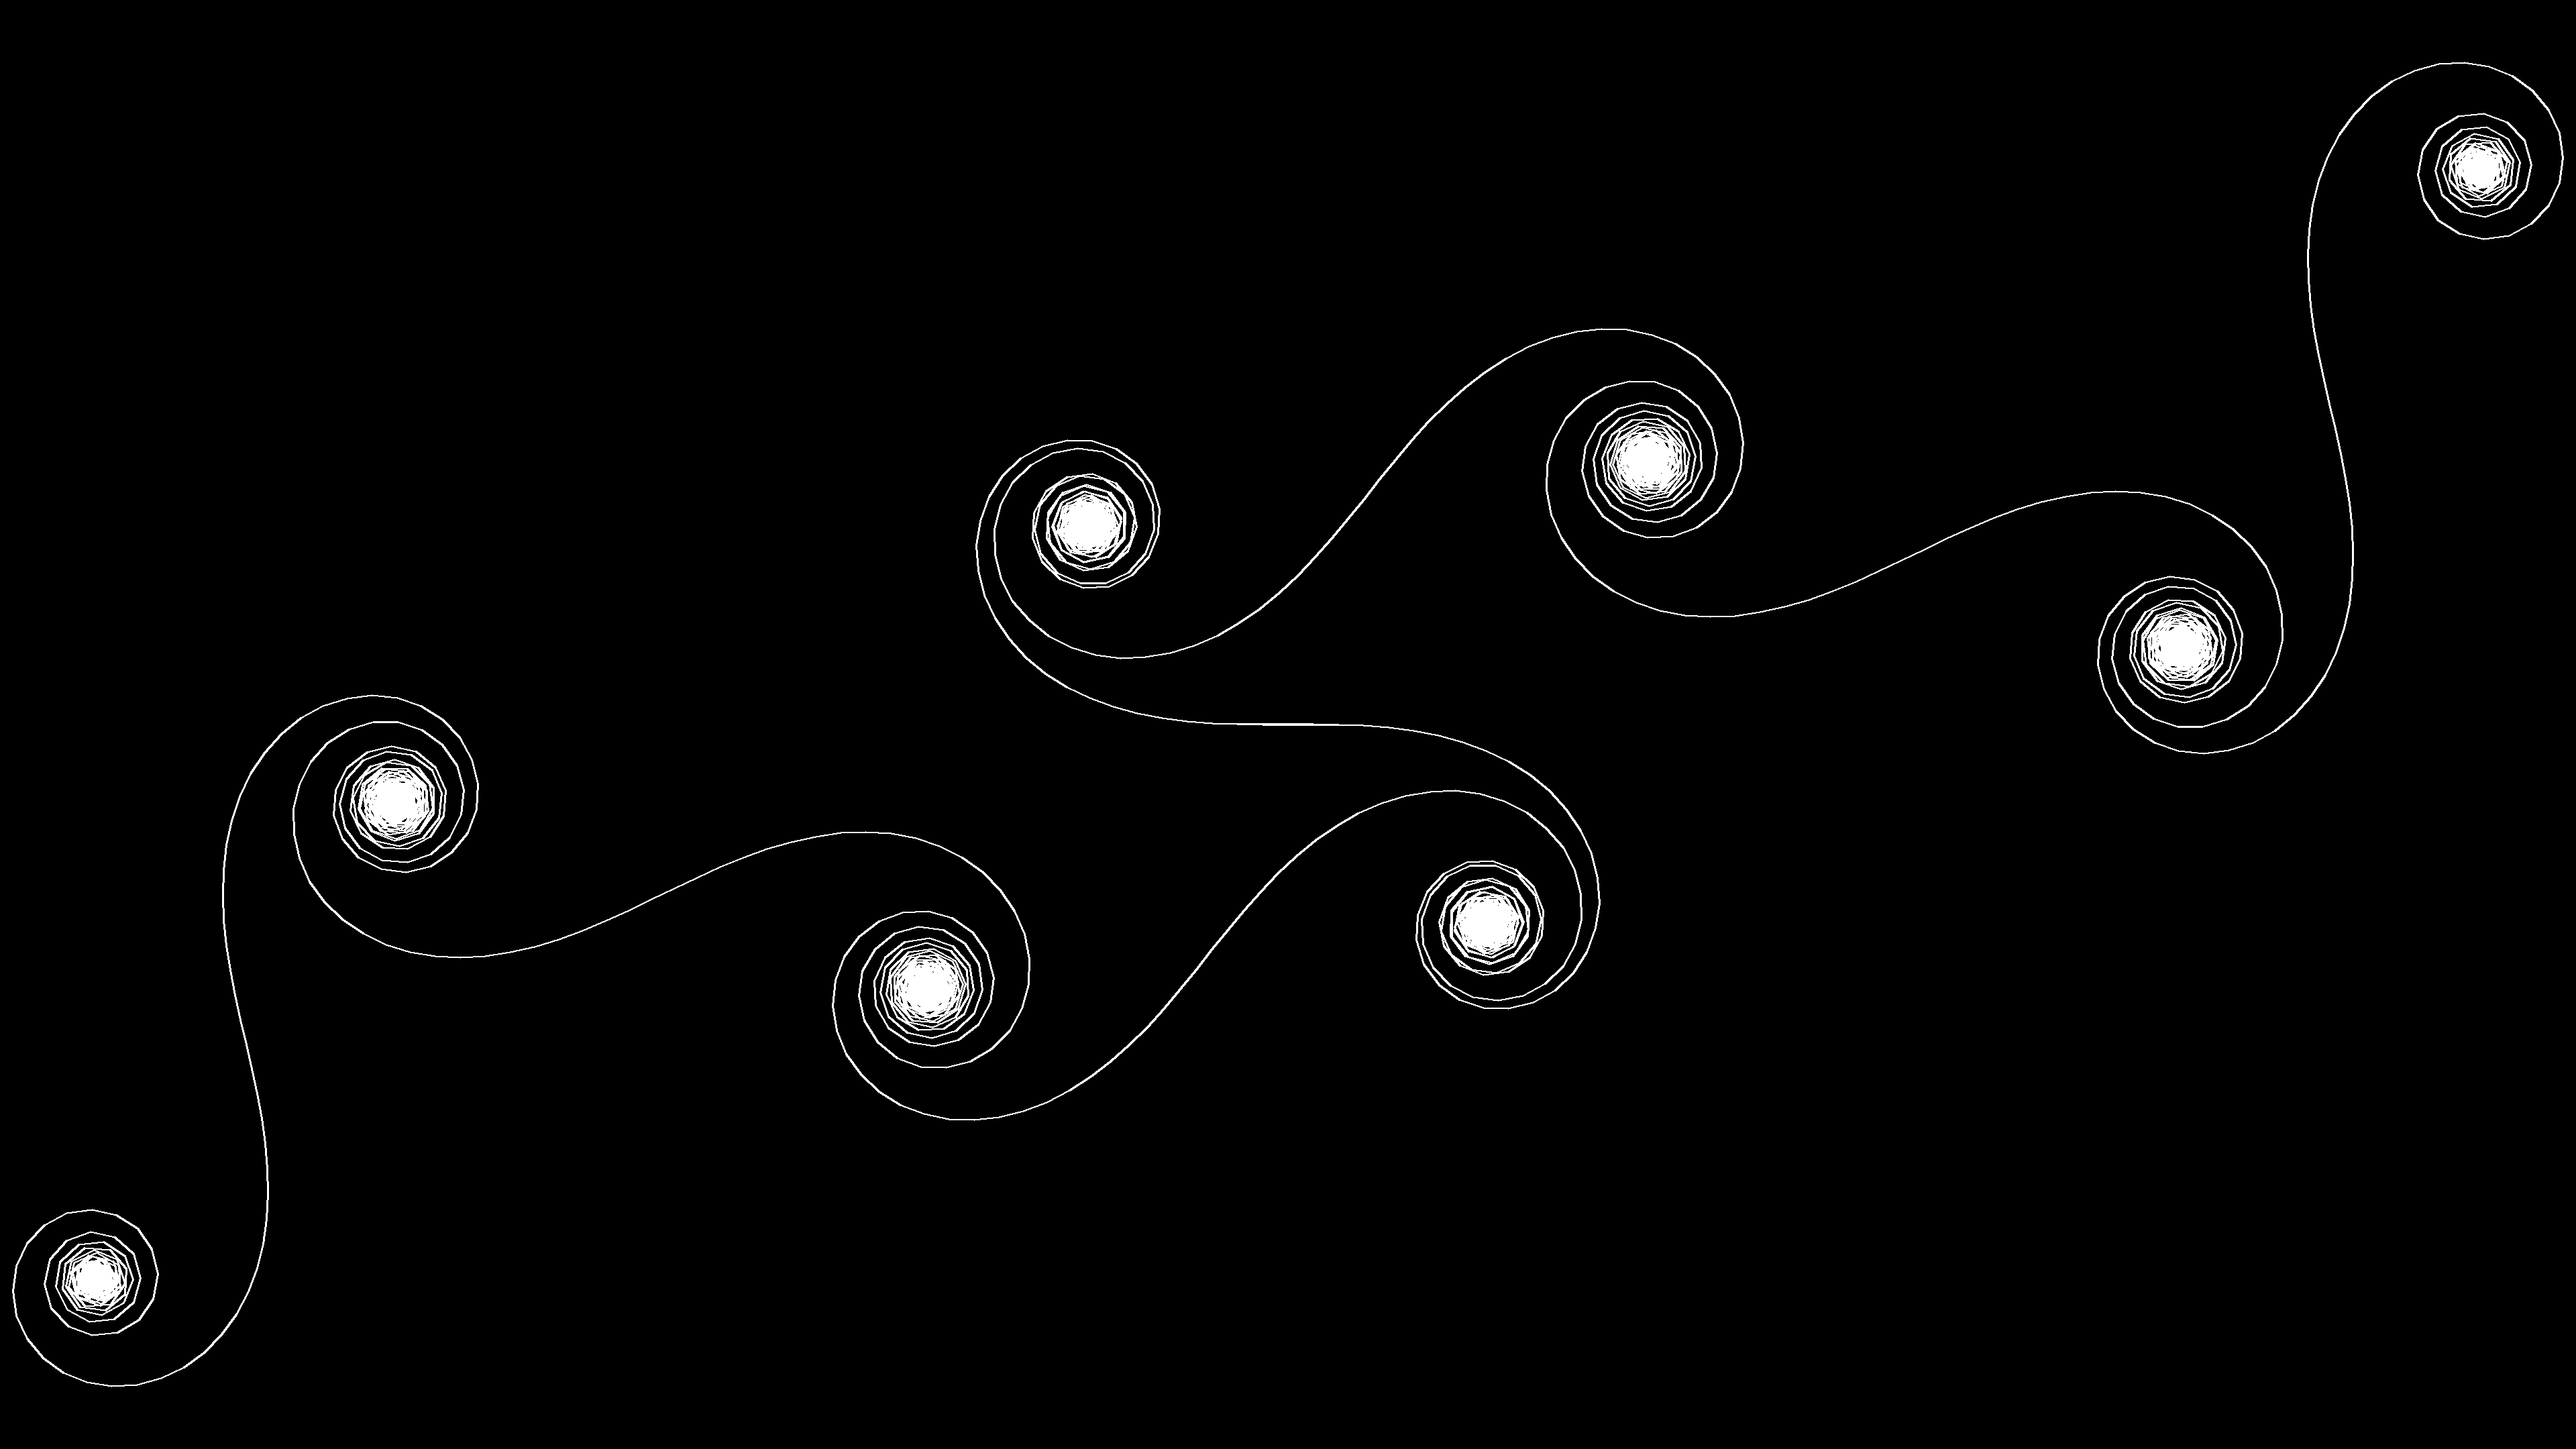
\includegraphics[width=0.3\textwidth]{tf_p=7--q=3502--theta=000_71958881.png}
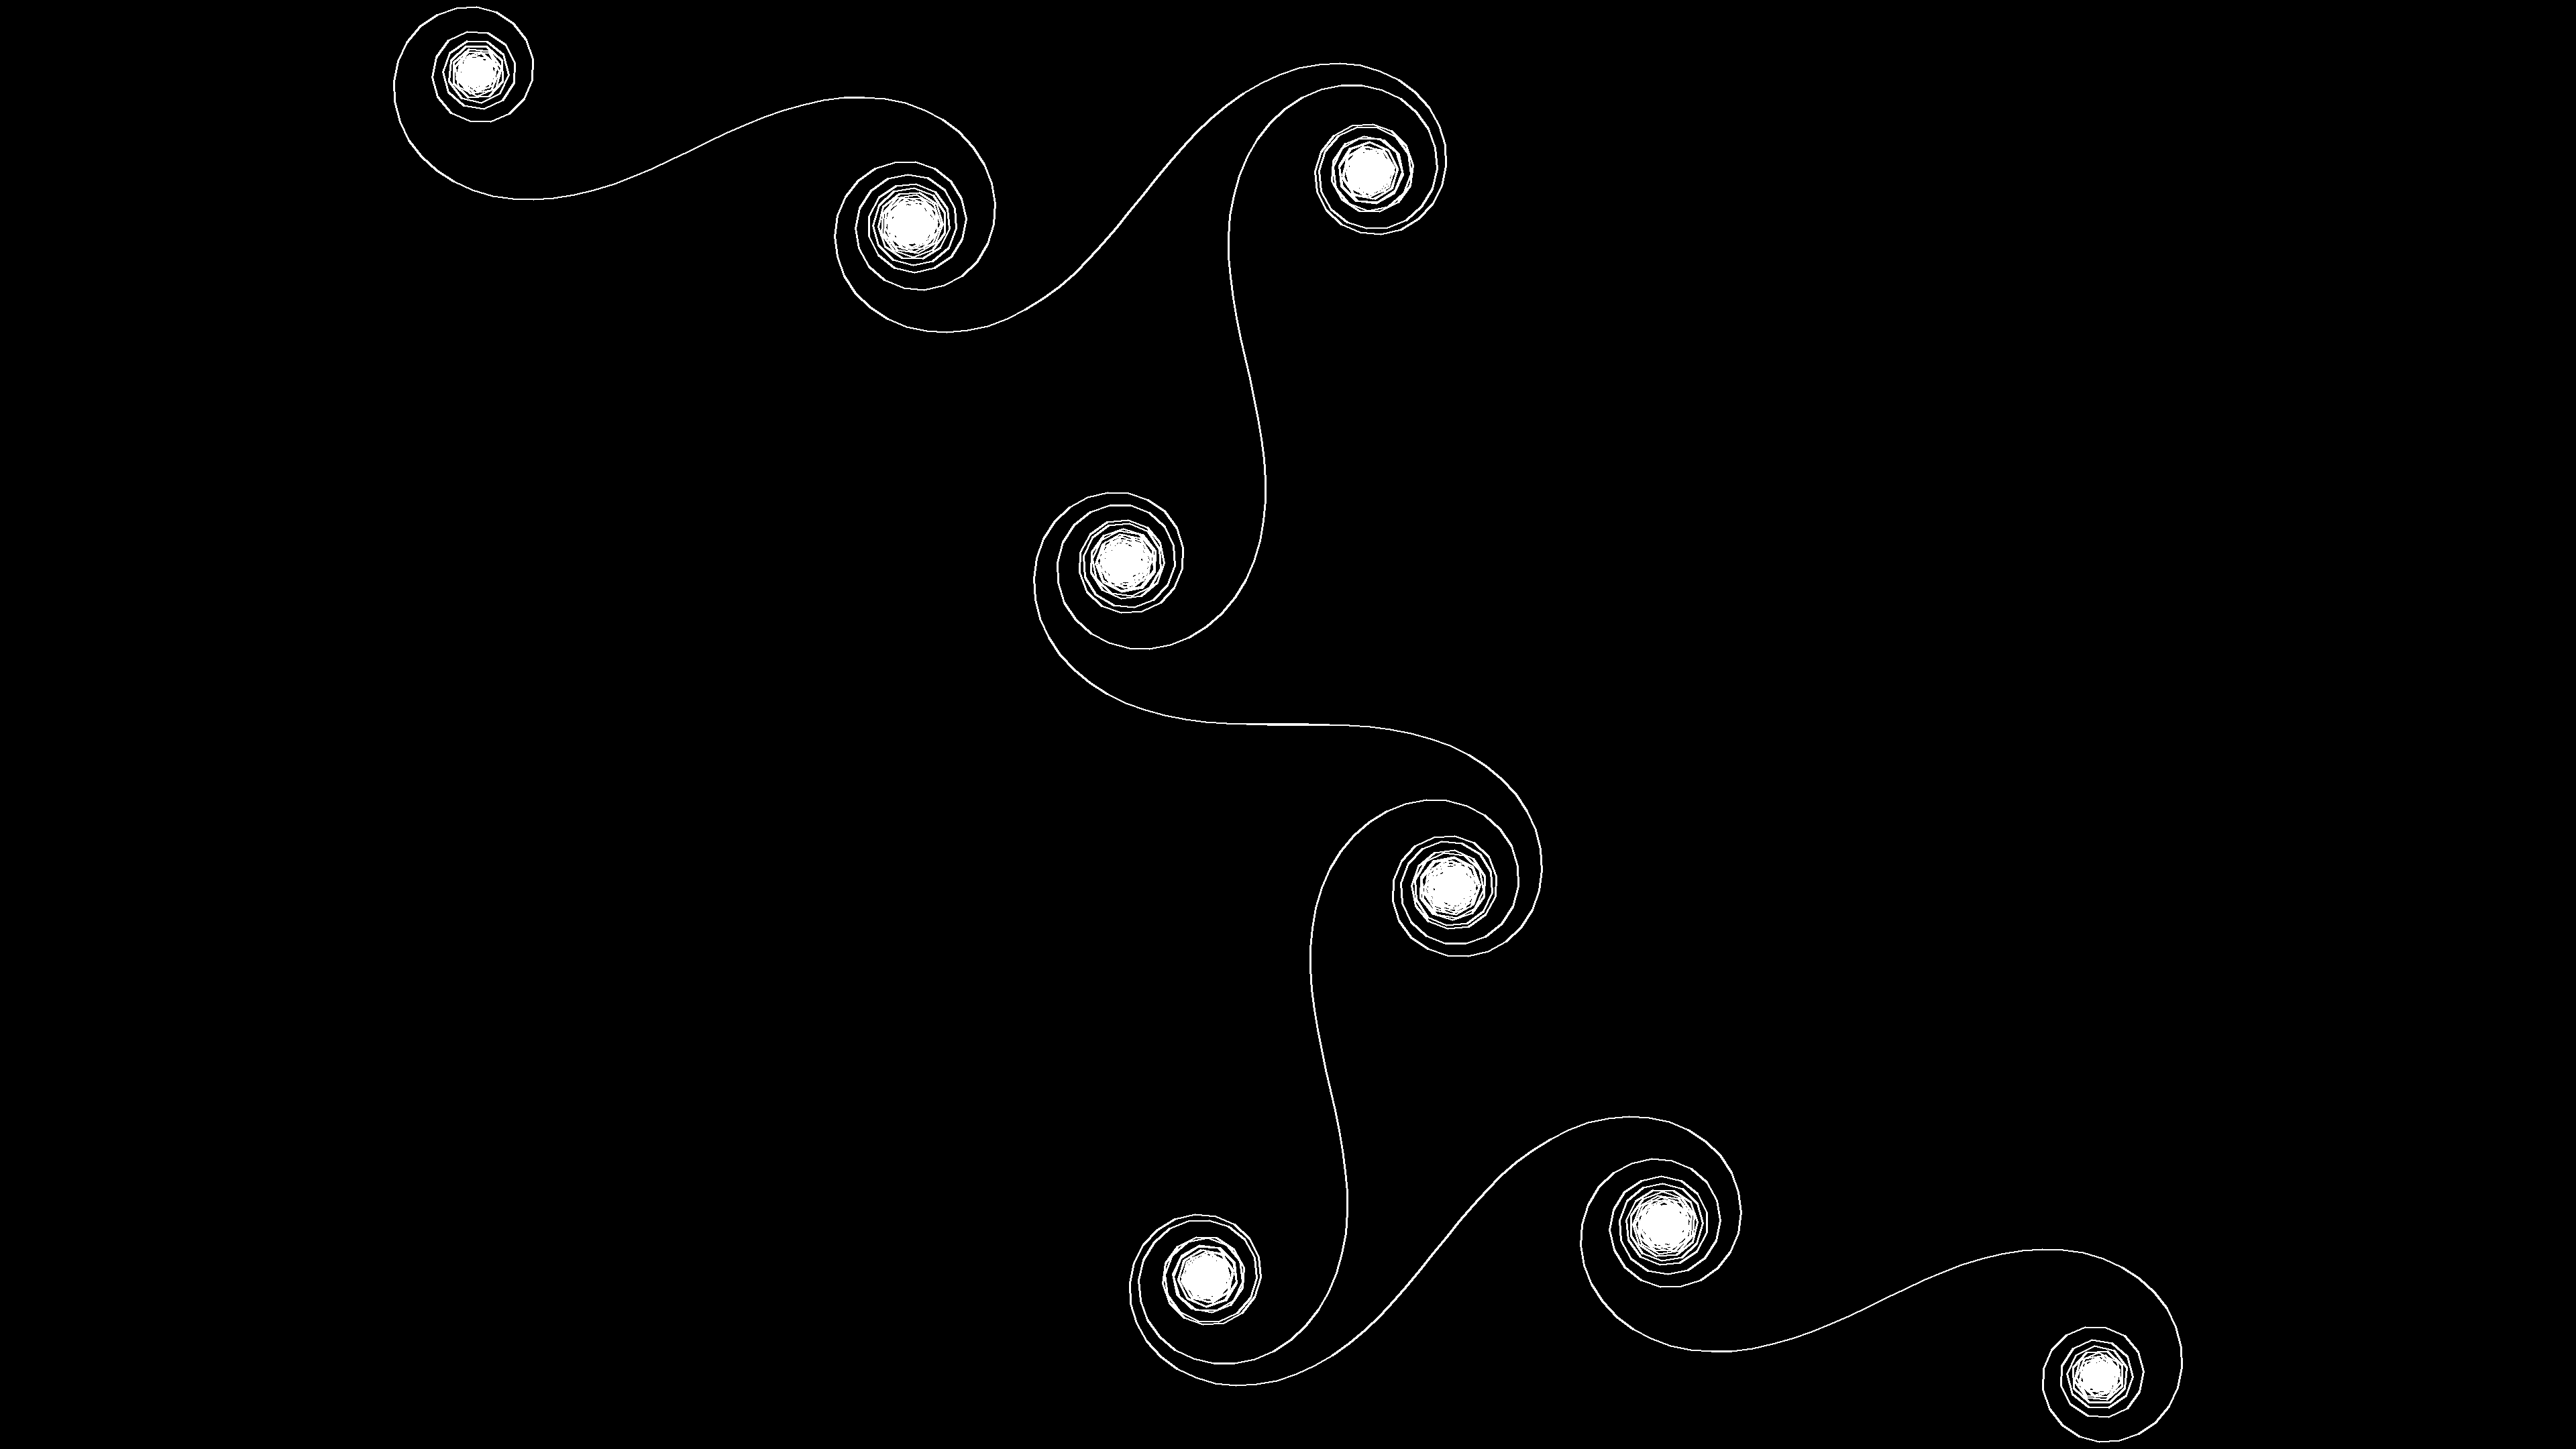
\includegraphics[width=0.3\textwidth]{tf_p=7--q=3504--theta=000_71917808.png}
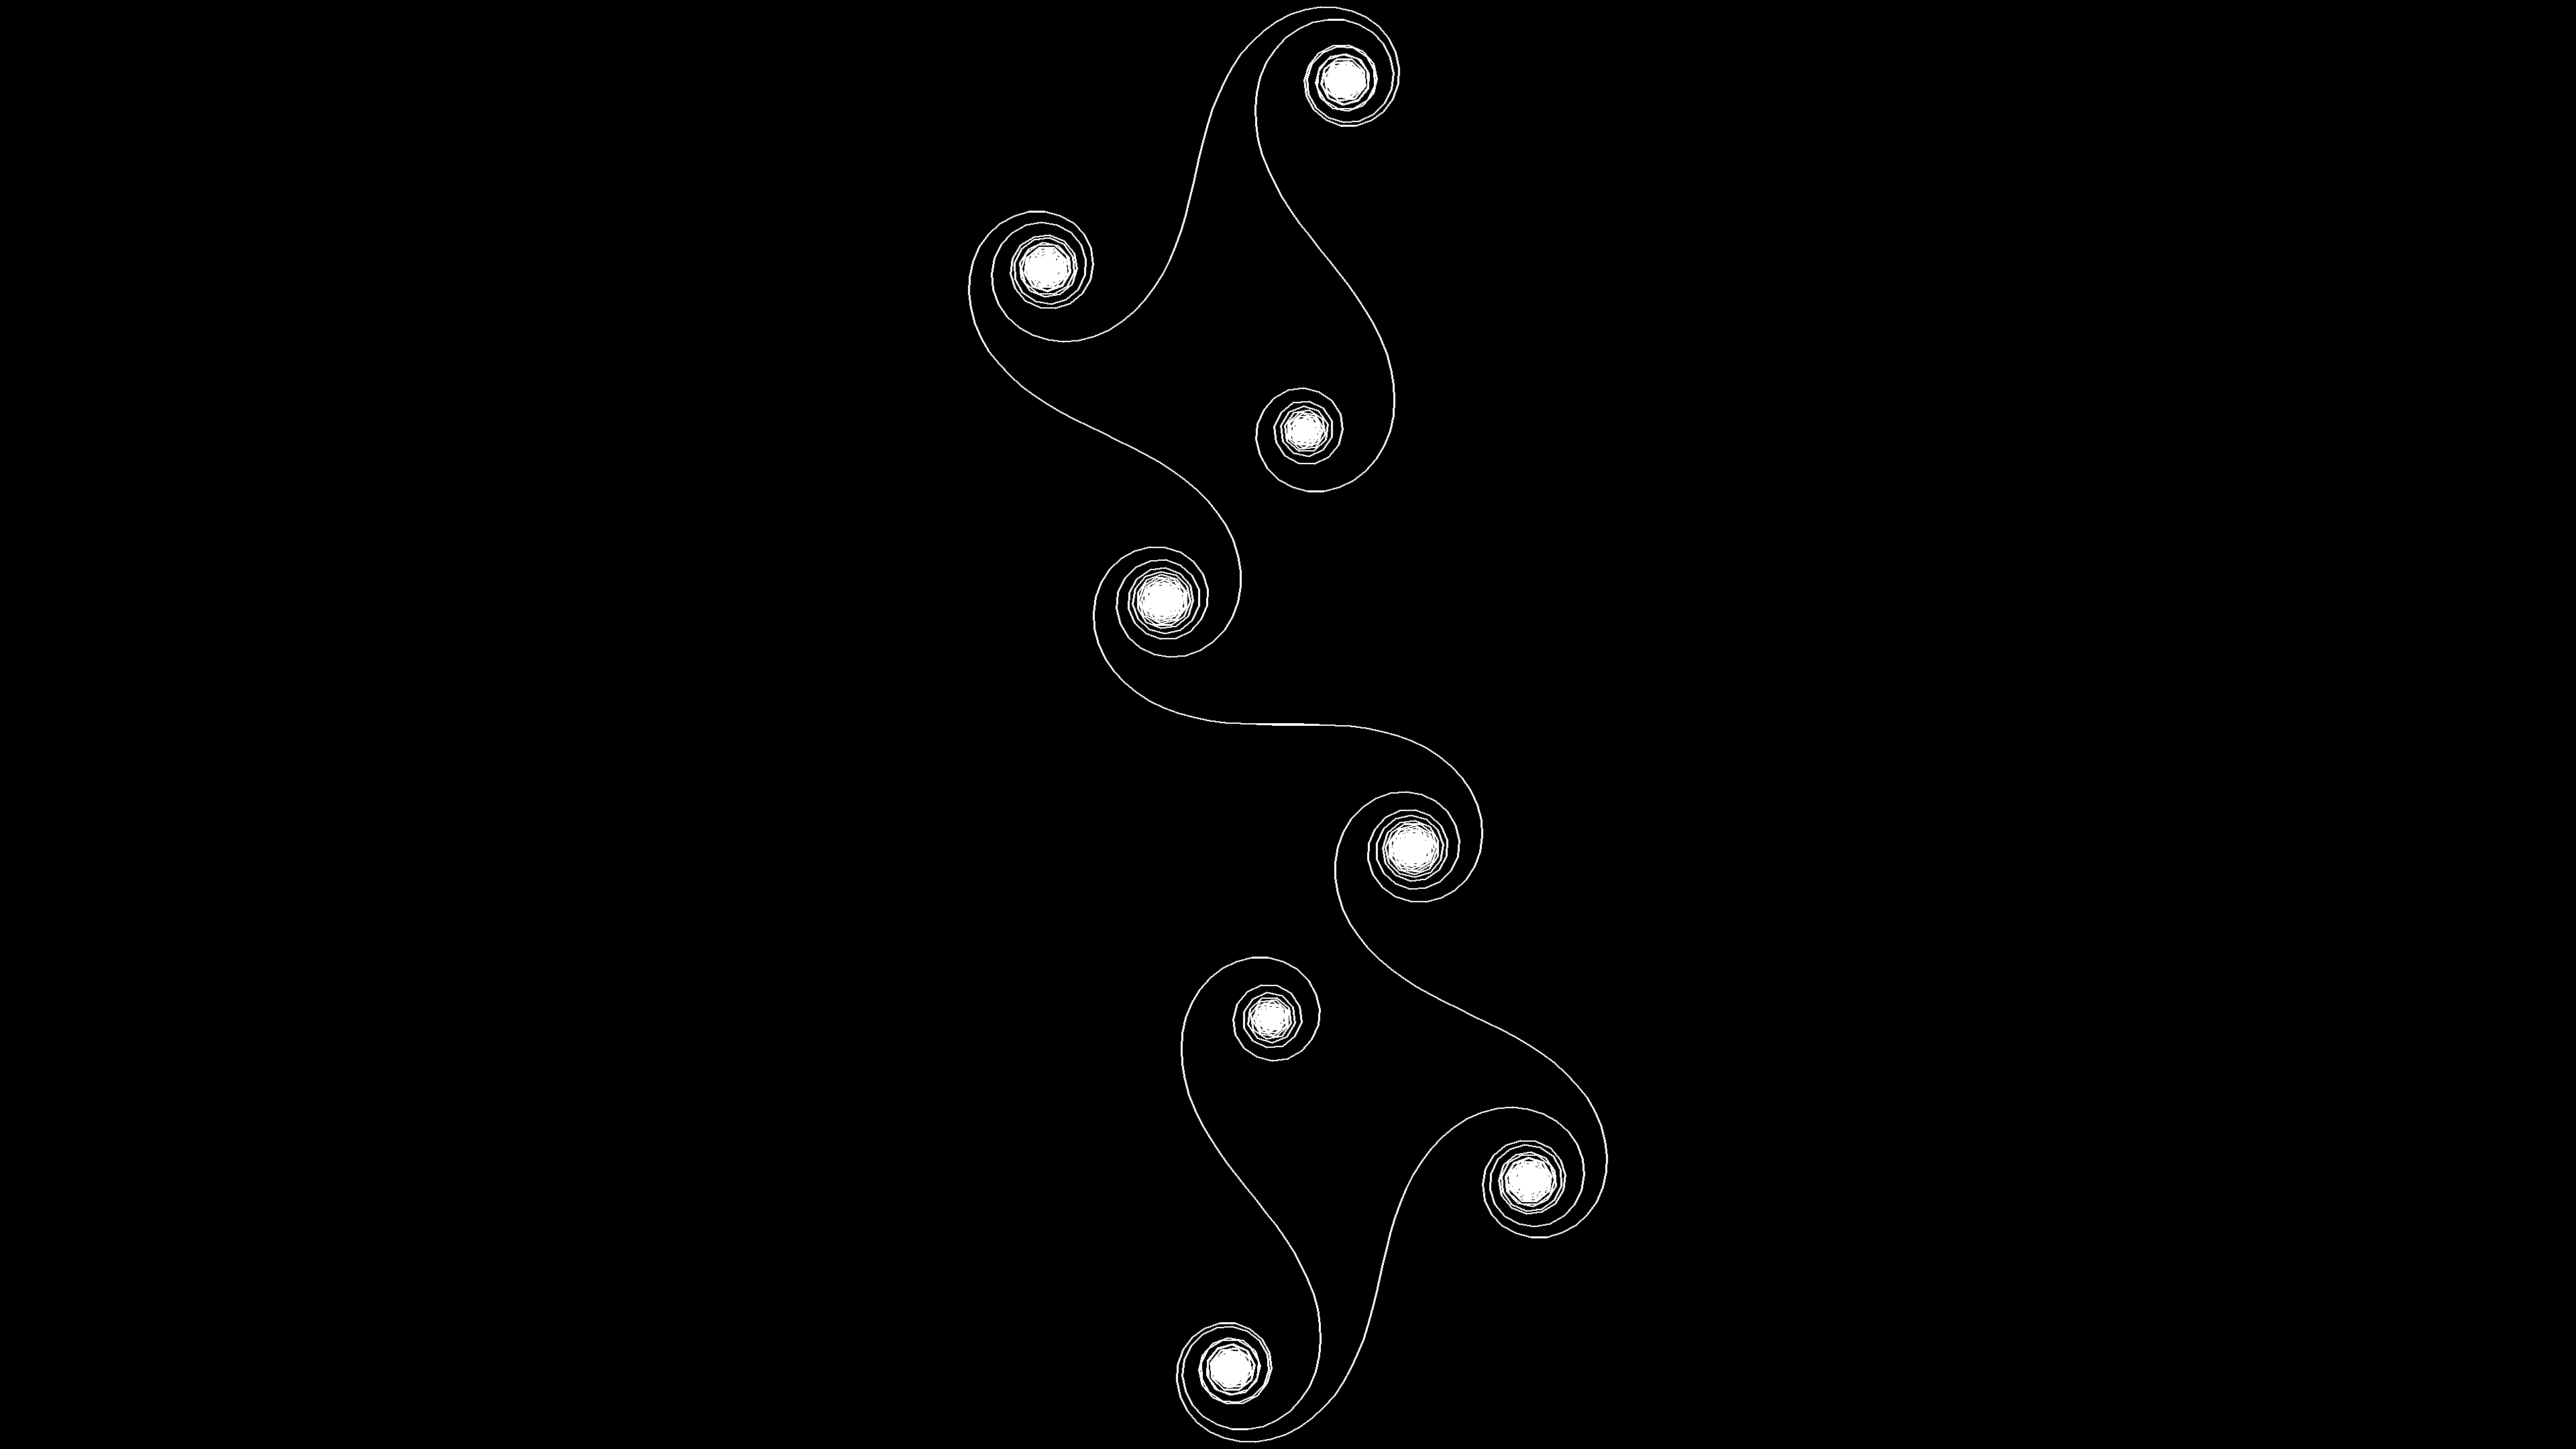
\includegraphics[width=0.3\textwidth]{tf_p=7--q=3506--theta=000_71876783.png}


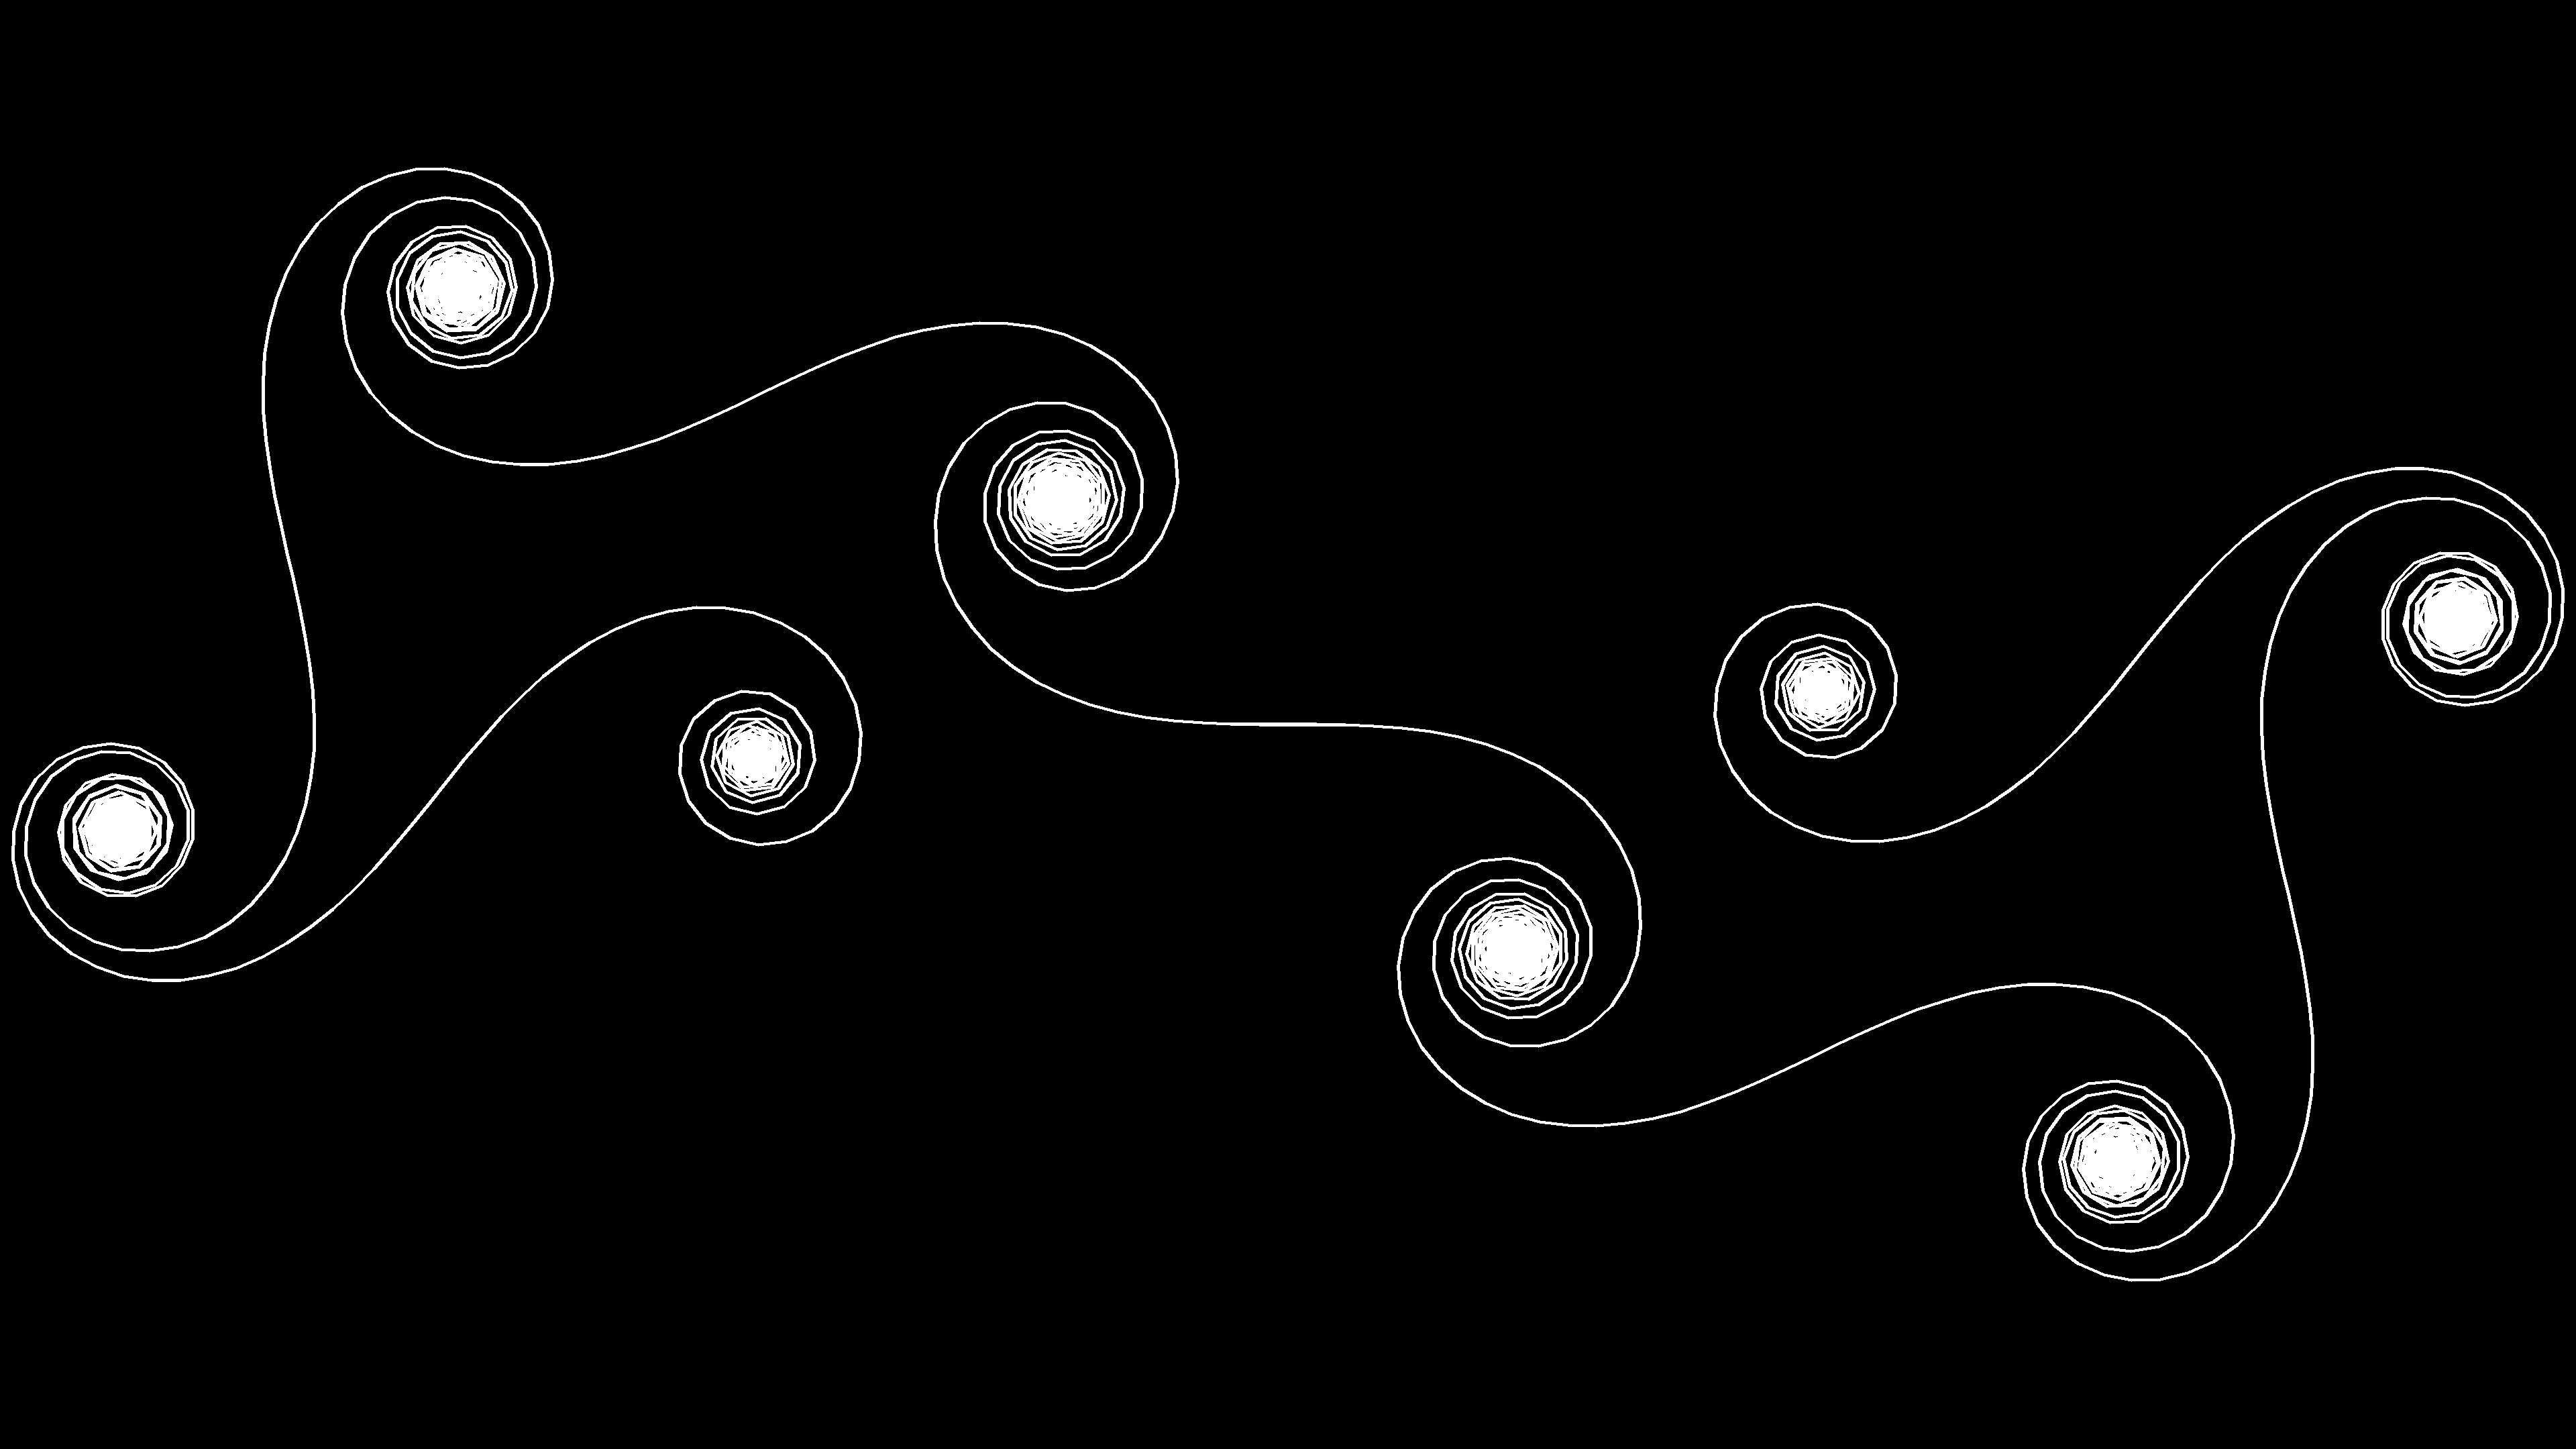
\includegraphics[width=0.3\textwidth]{tf_p=7--q=3508--theta=000_71835804.png}
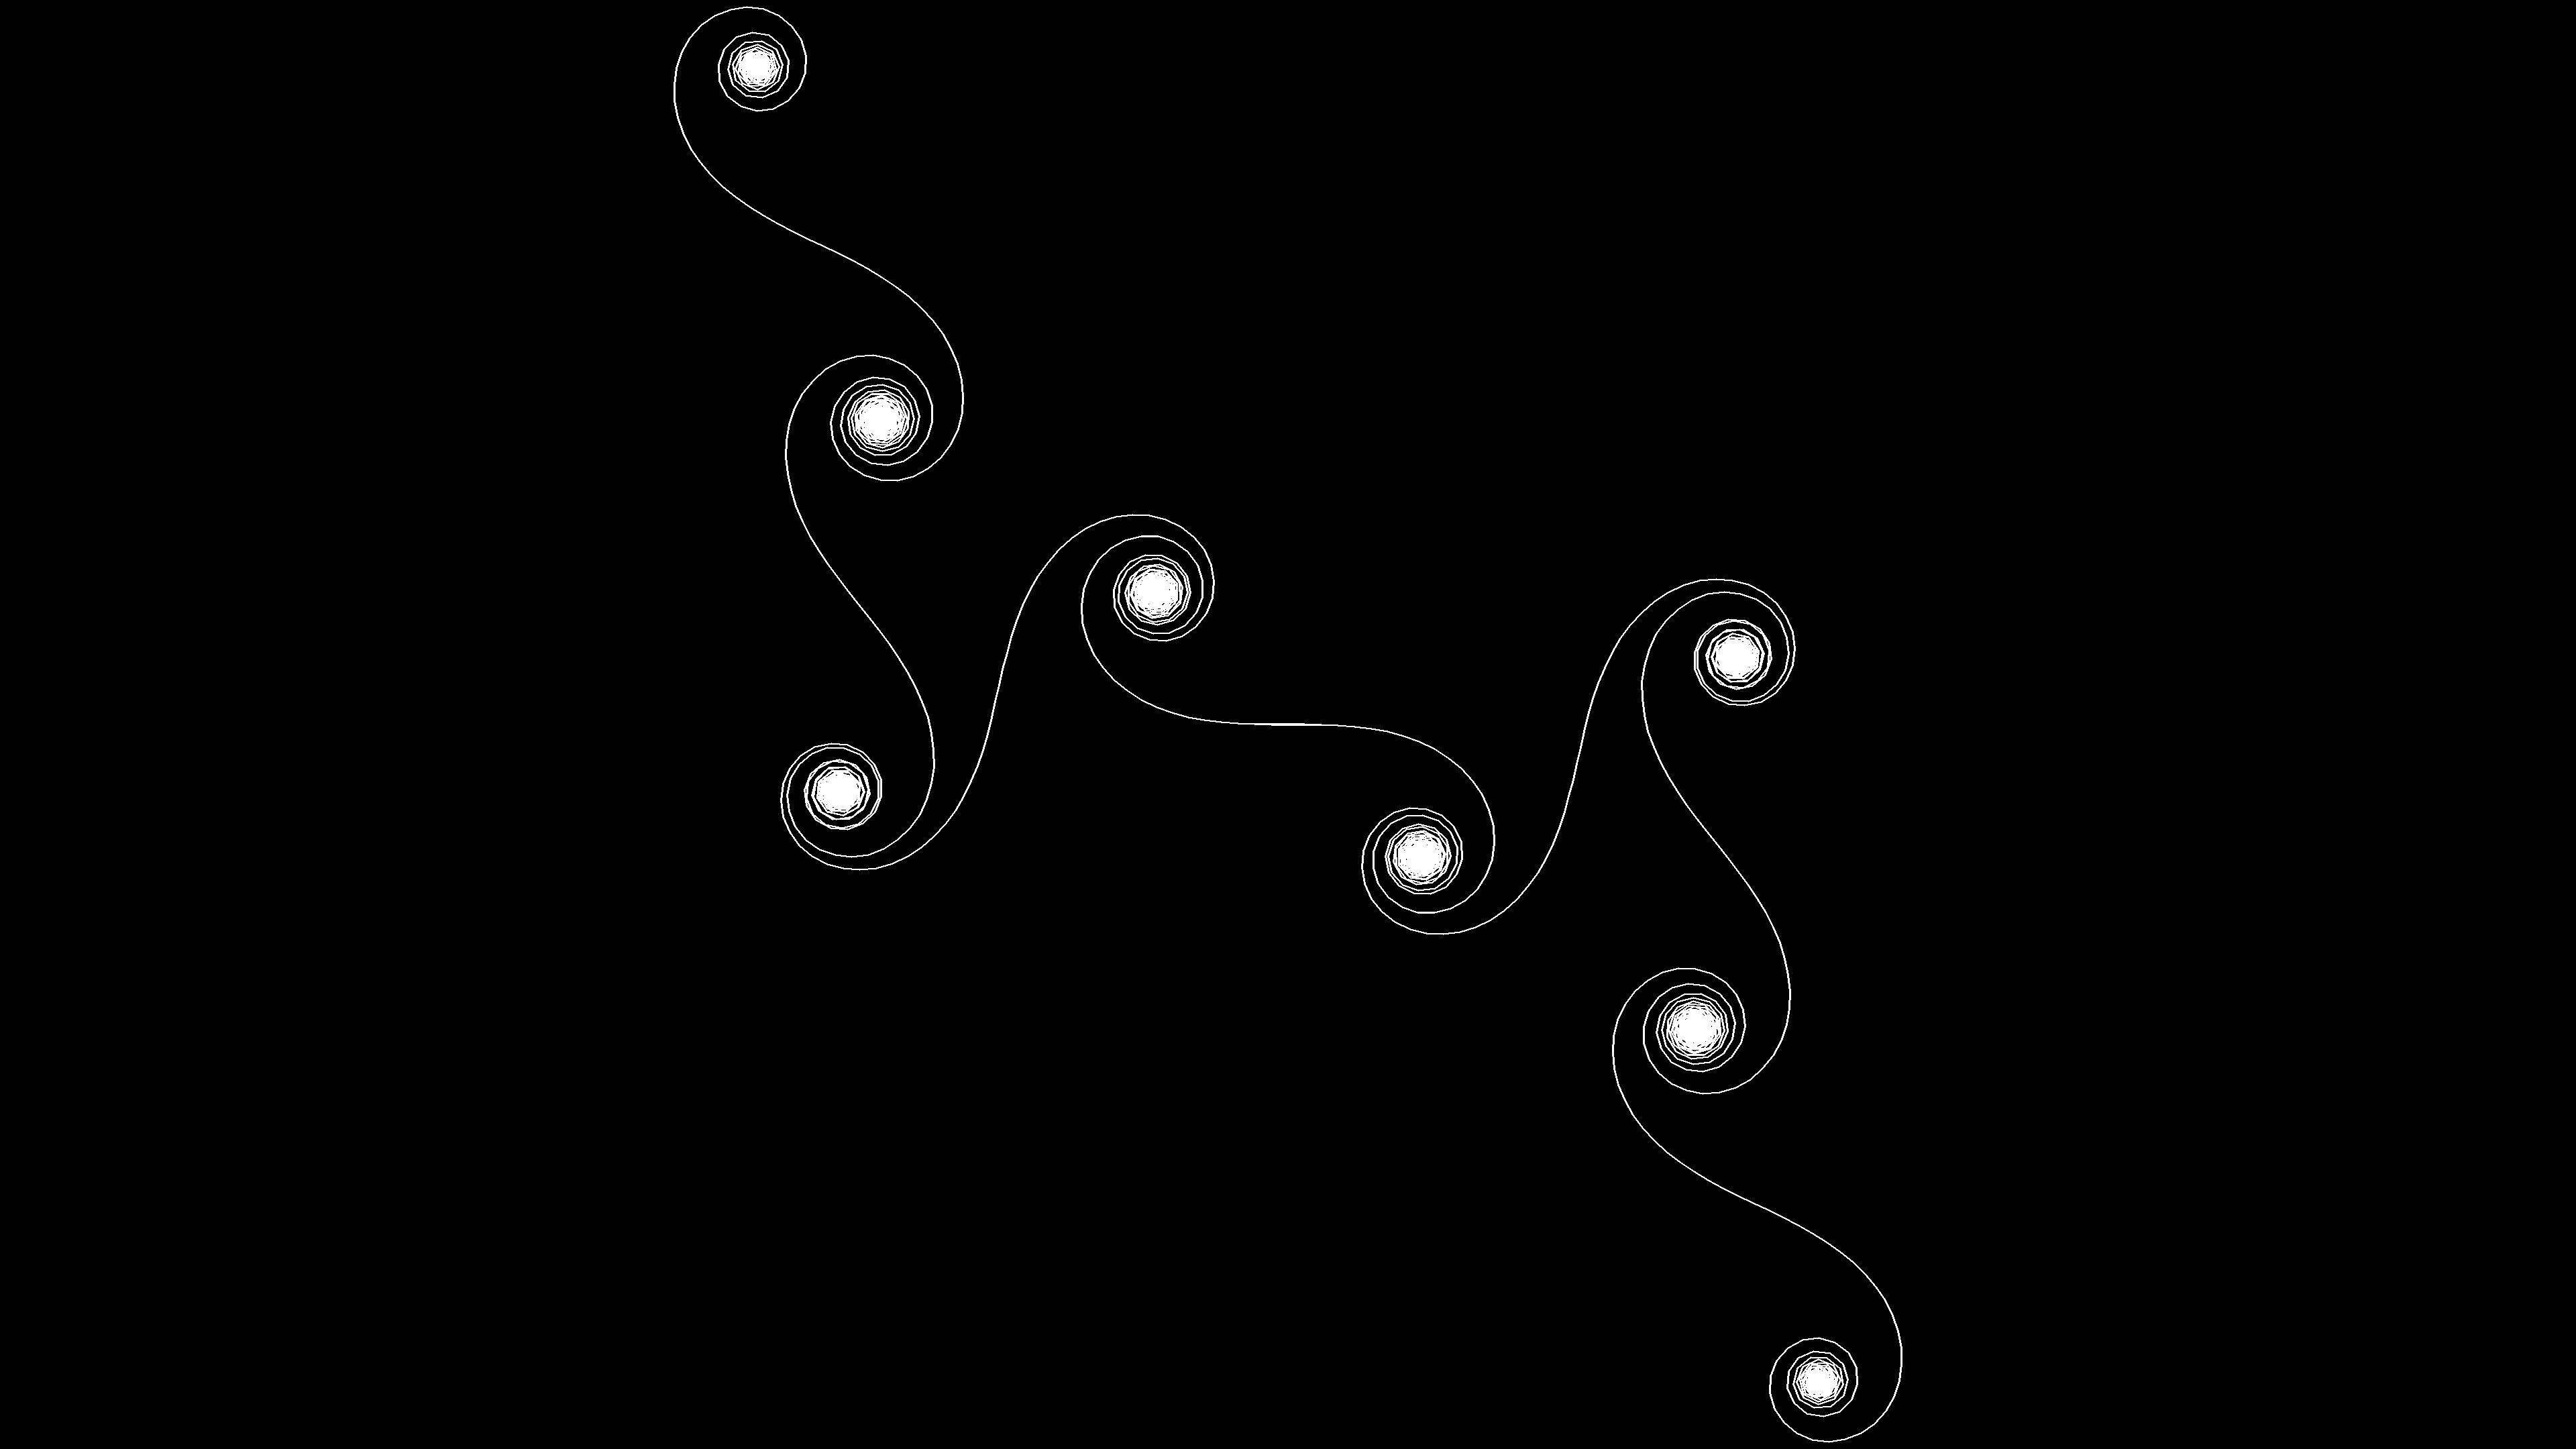
\includegraphics[width=0.3\textwidth]{tf_p=7--q=3510--theta=000_71794872.png}
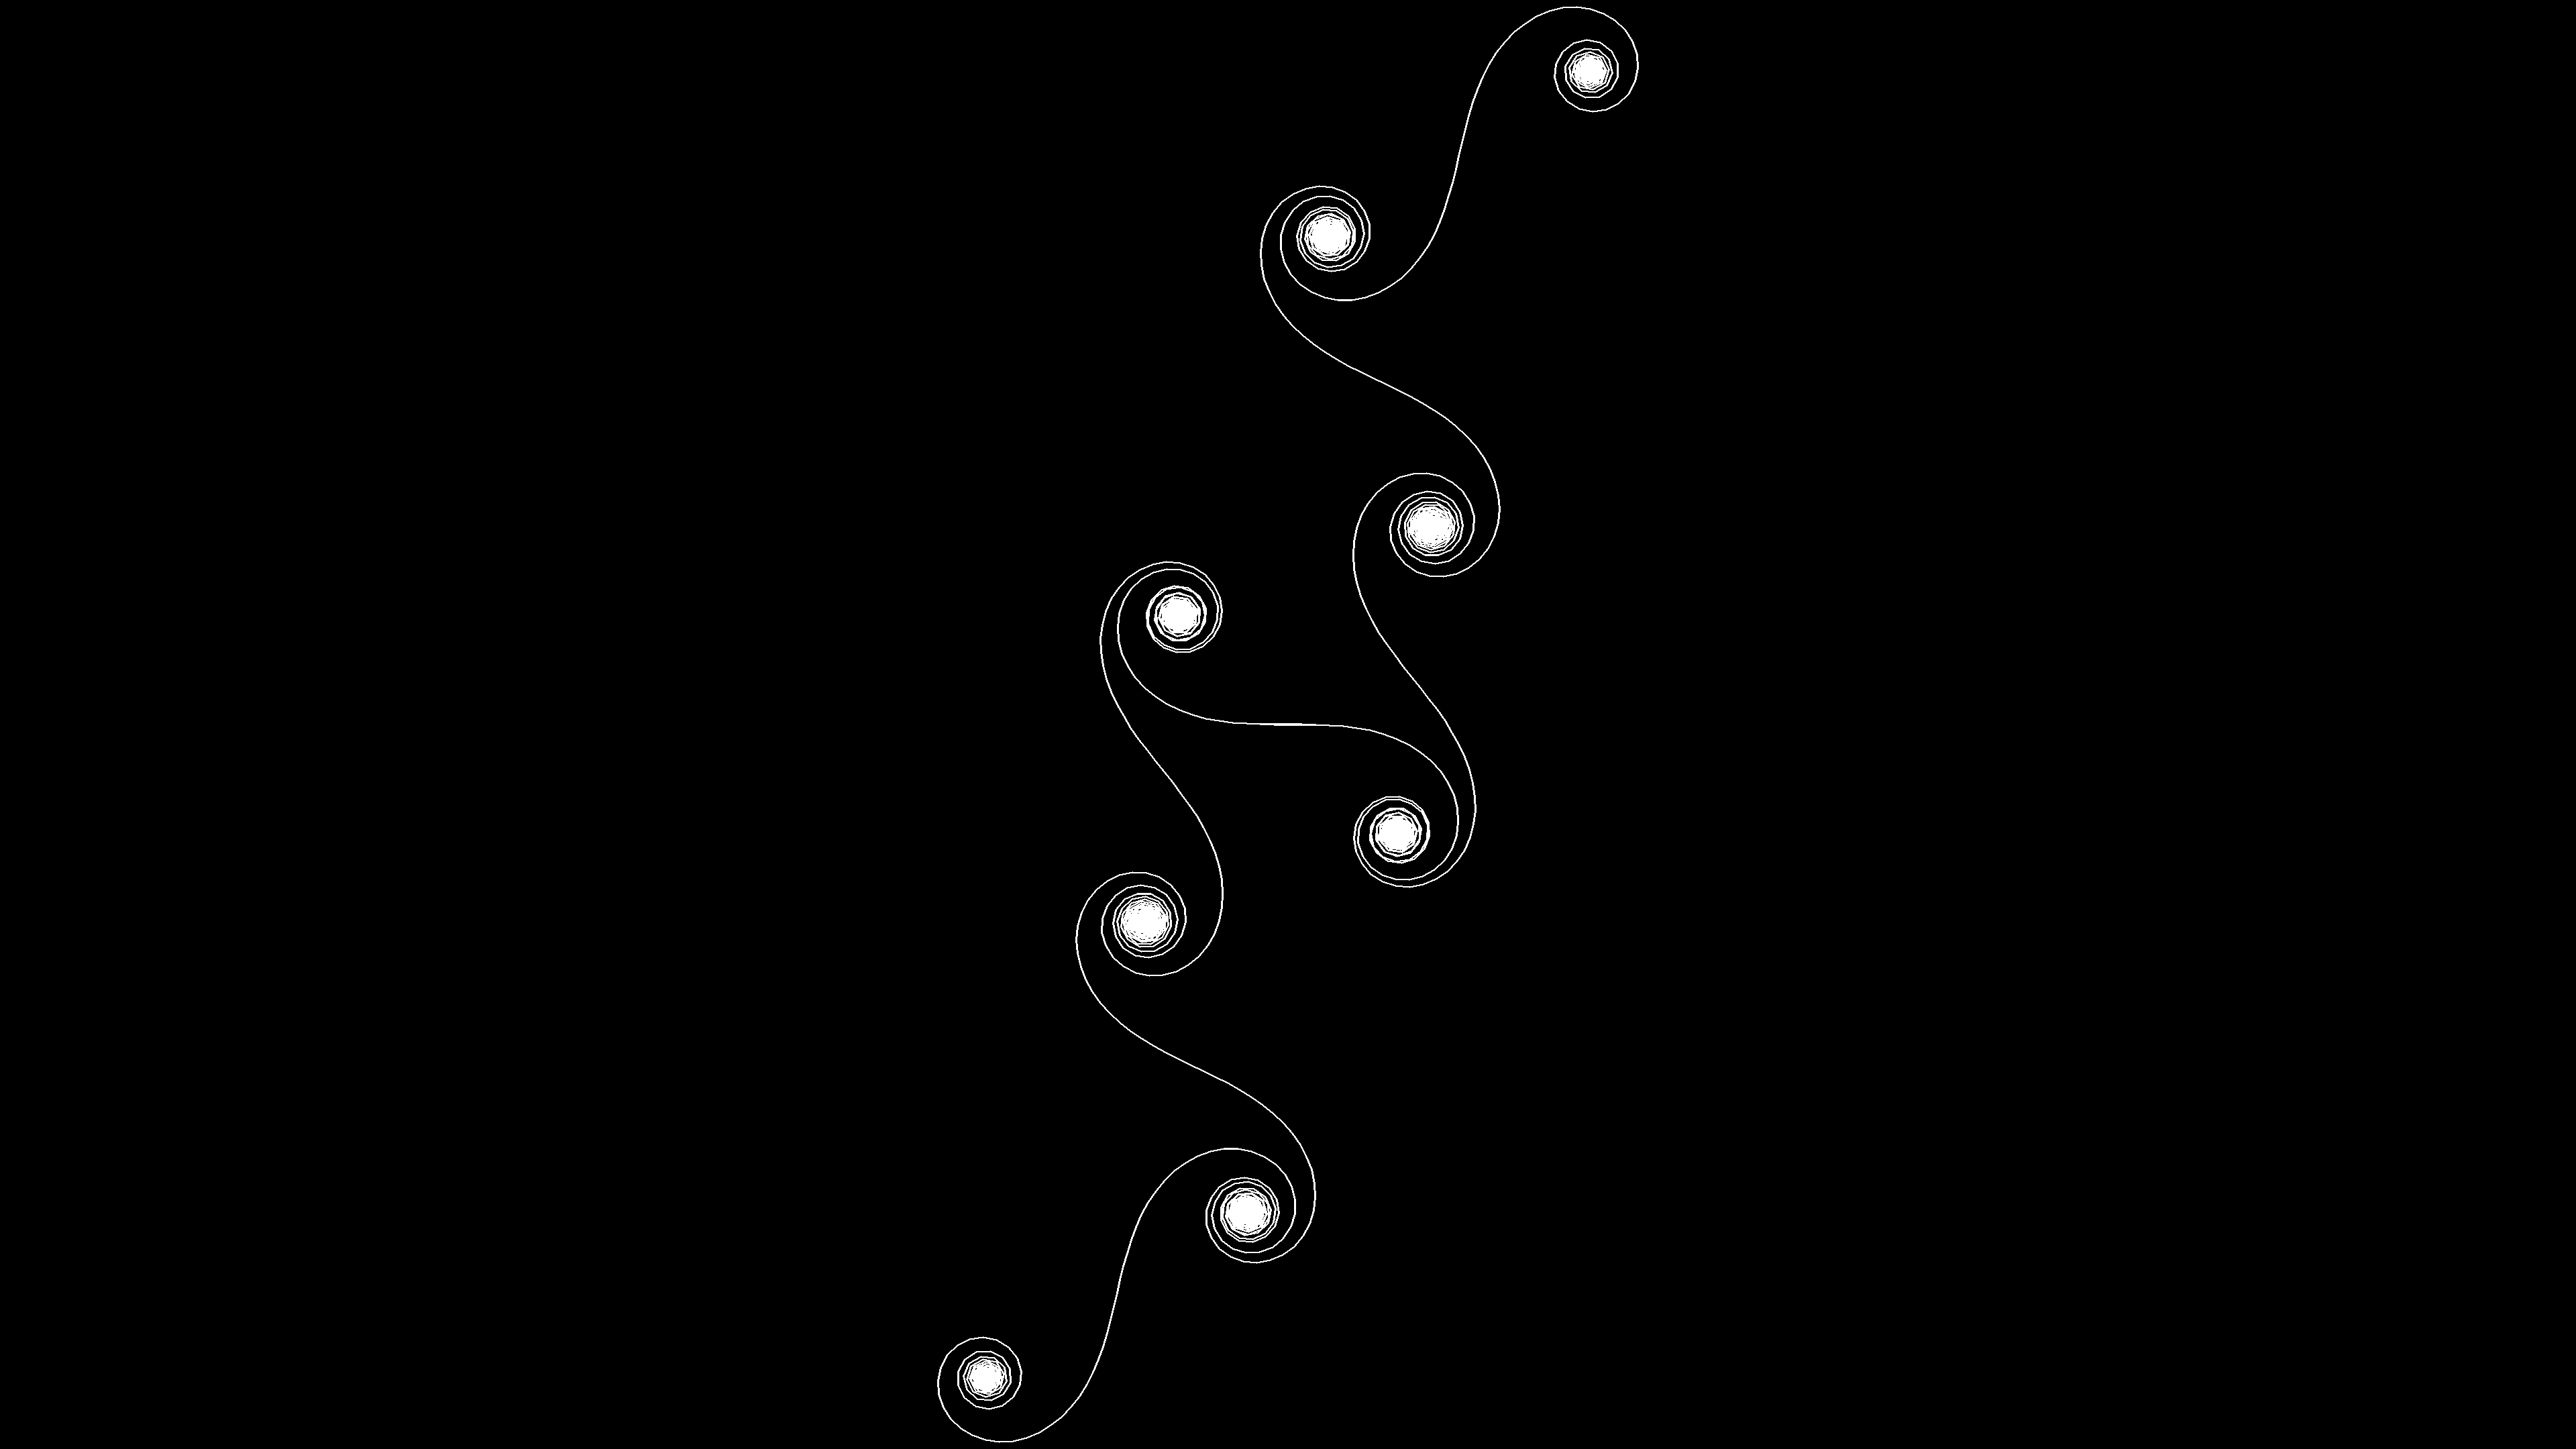
\includegraphics[width=0.3\textwidth]{tf_p=7--q=3512--theta=000_71753986.png}

This number of images per $p$ can only be achieved for prime numbers. Non prime numbers create less images due to the coprime
restriction of $p$ and $q$.

Adding $2 \cdot p$ to $q$ creates the same base image, but with a higher 
'resolution', meaning a higher number of steps used to create the Euler spiral. In the following picture series, $p=89$ is
depicted for $q \in \{2, 180, 358, 536, 714, 892, 1070, 1248, ..., 49842\}$.

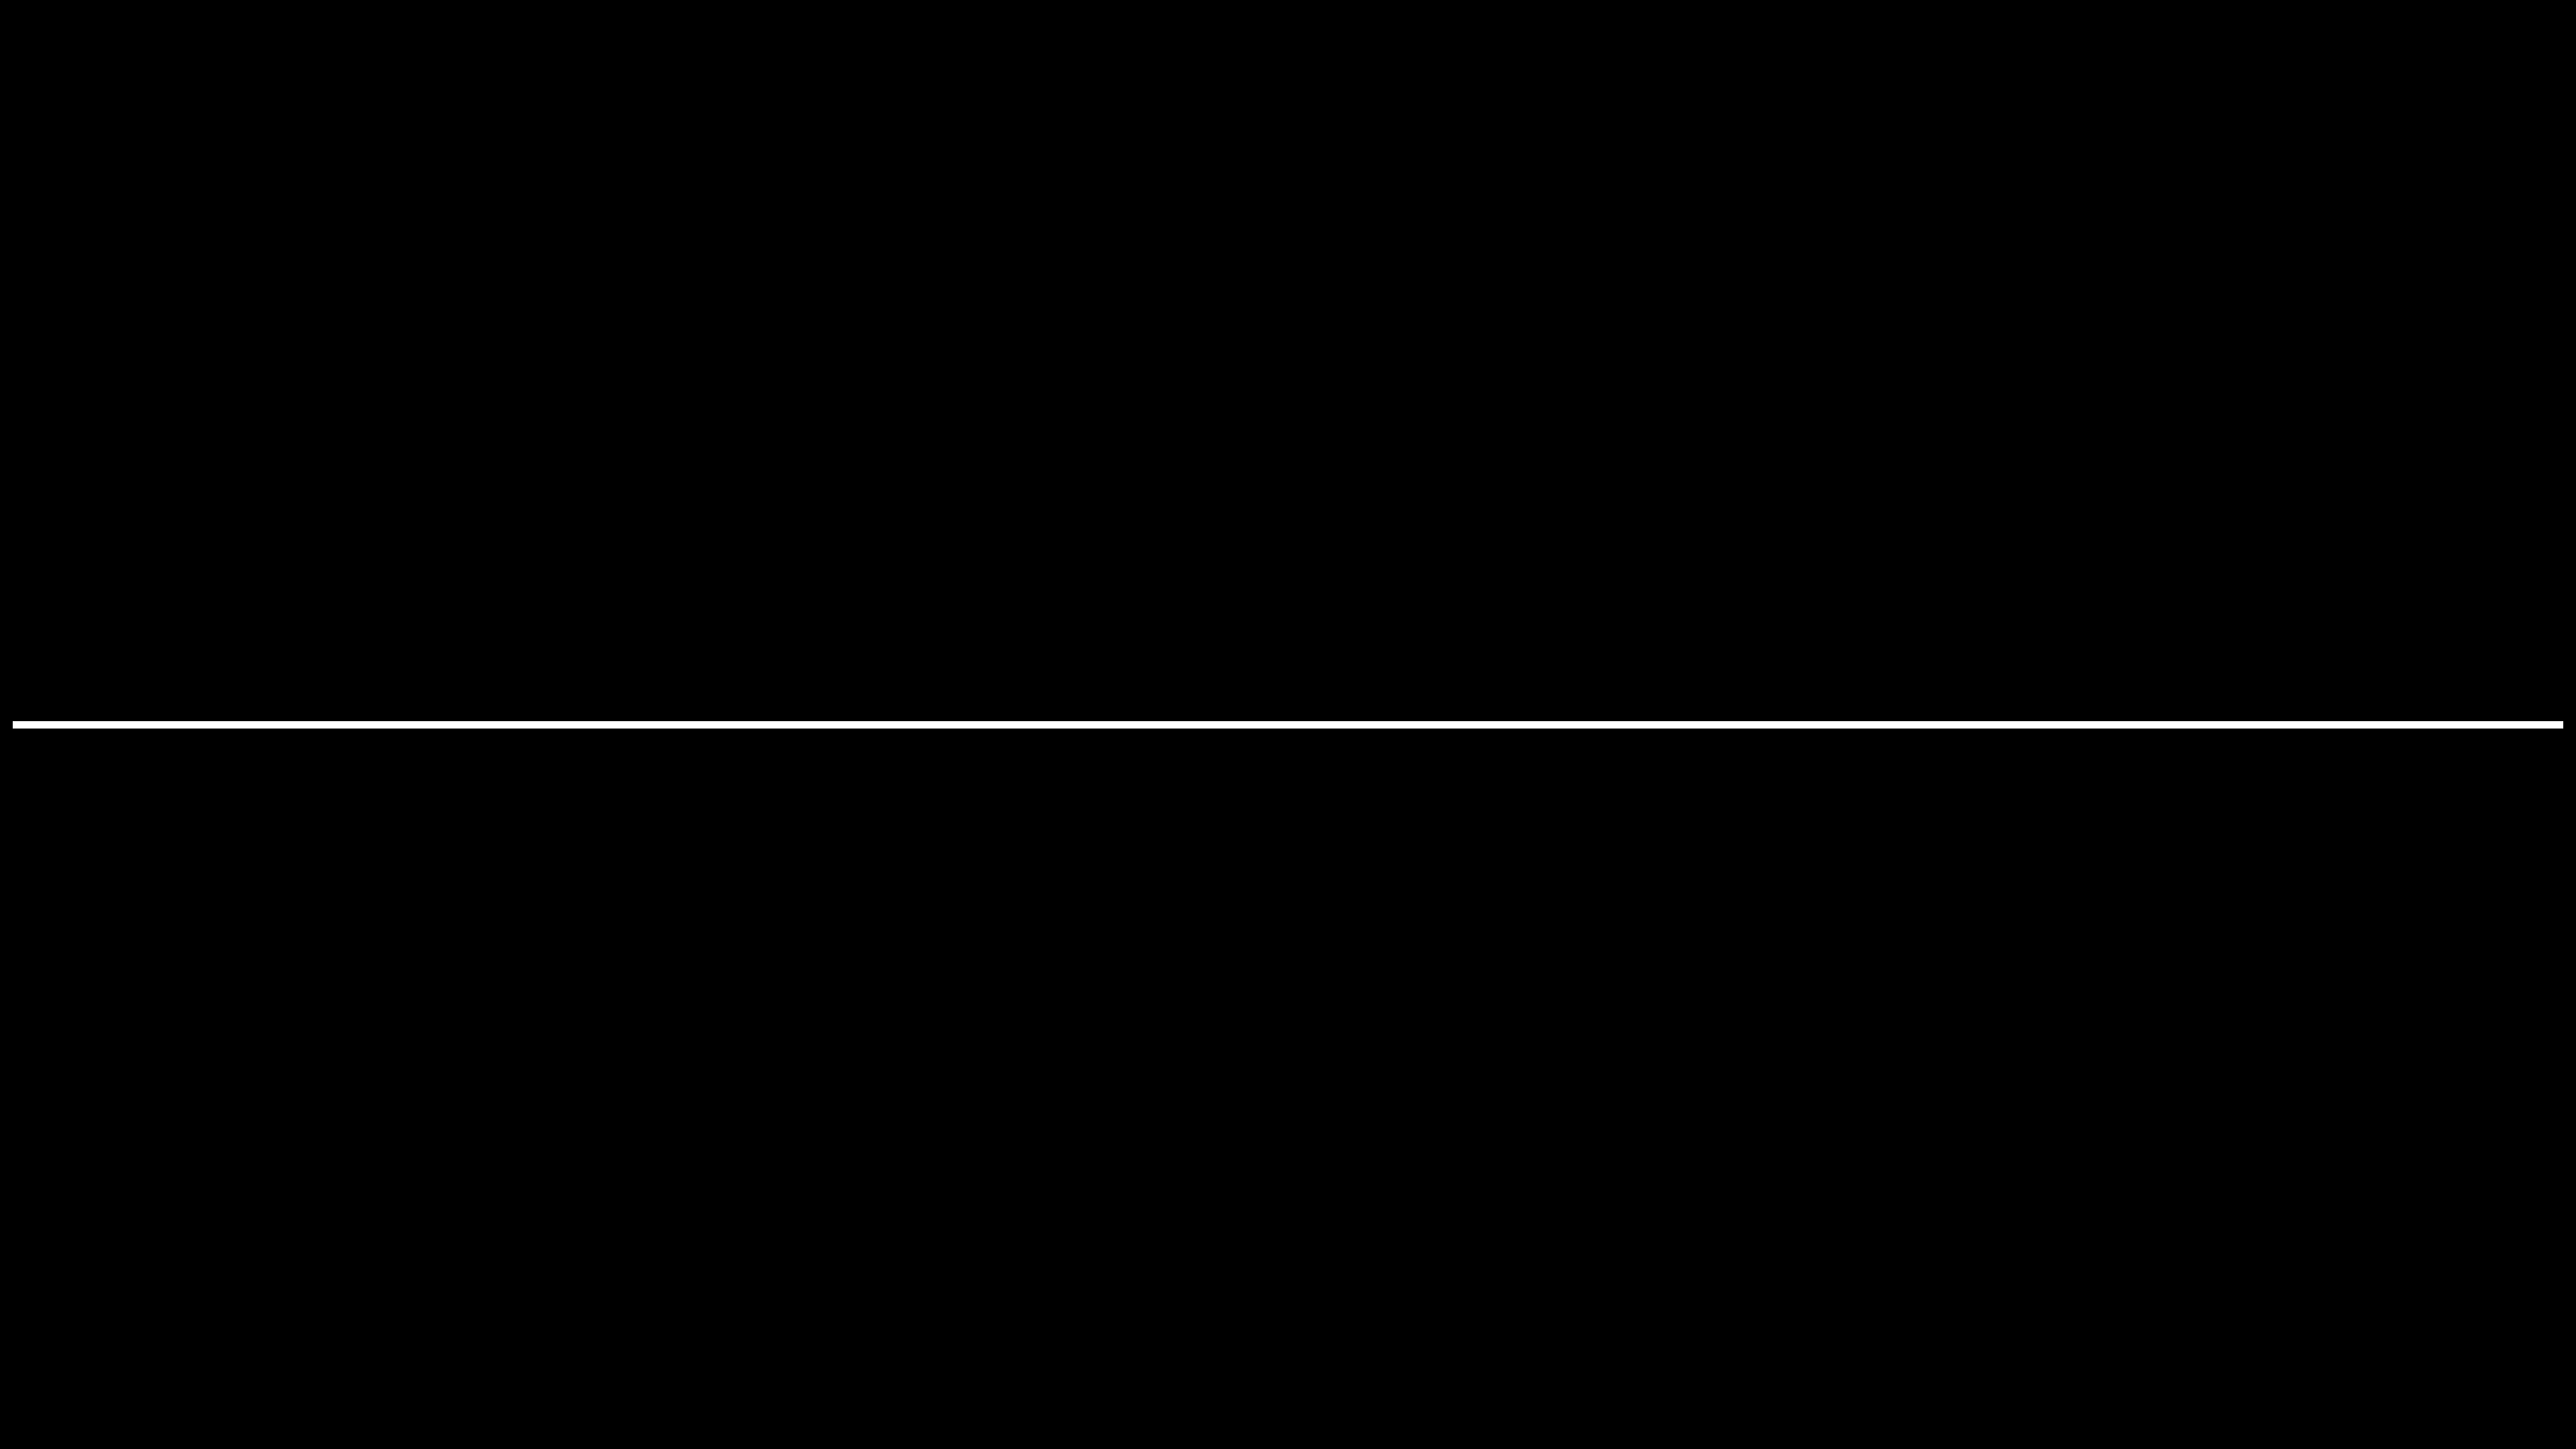
\includegraphics[width=0.3\textwidth]{tf_p=89--q=2--theta=16020_00000000.png}
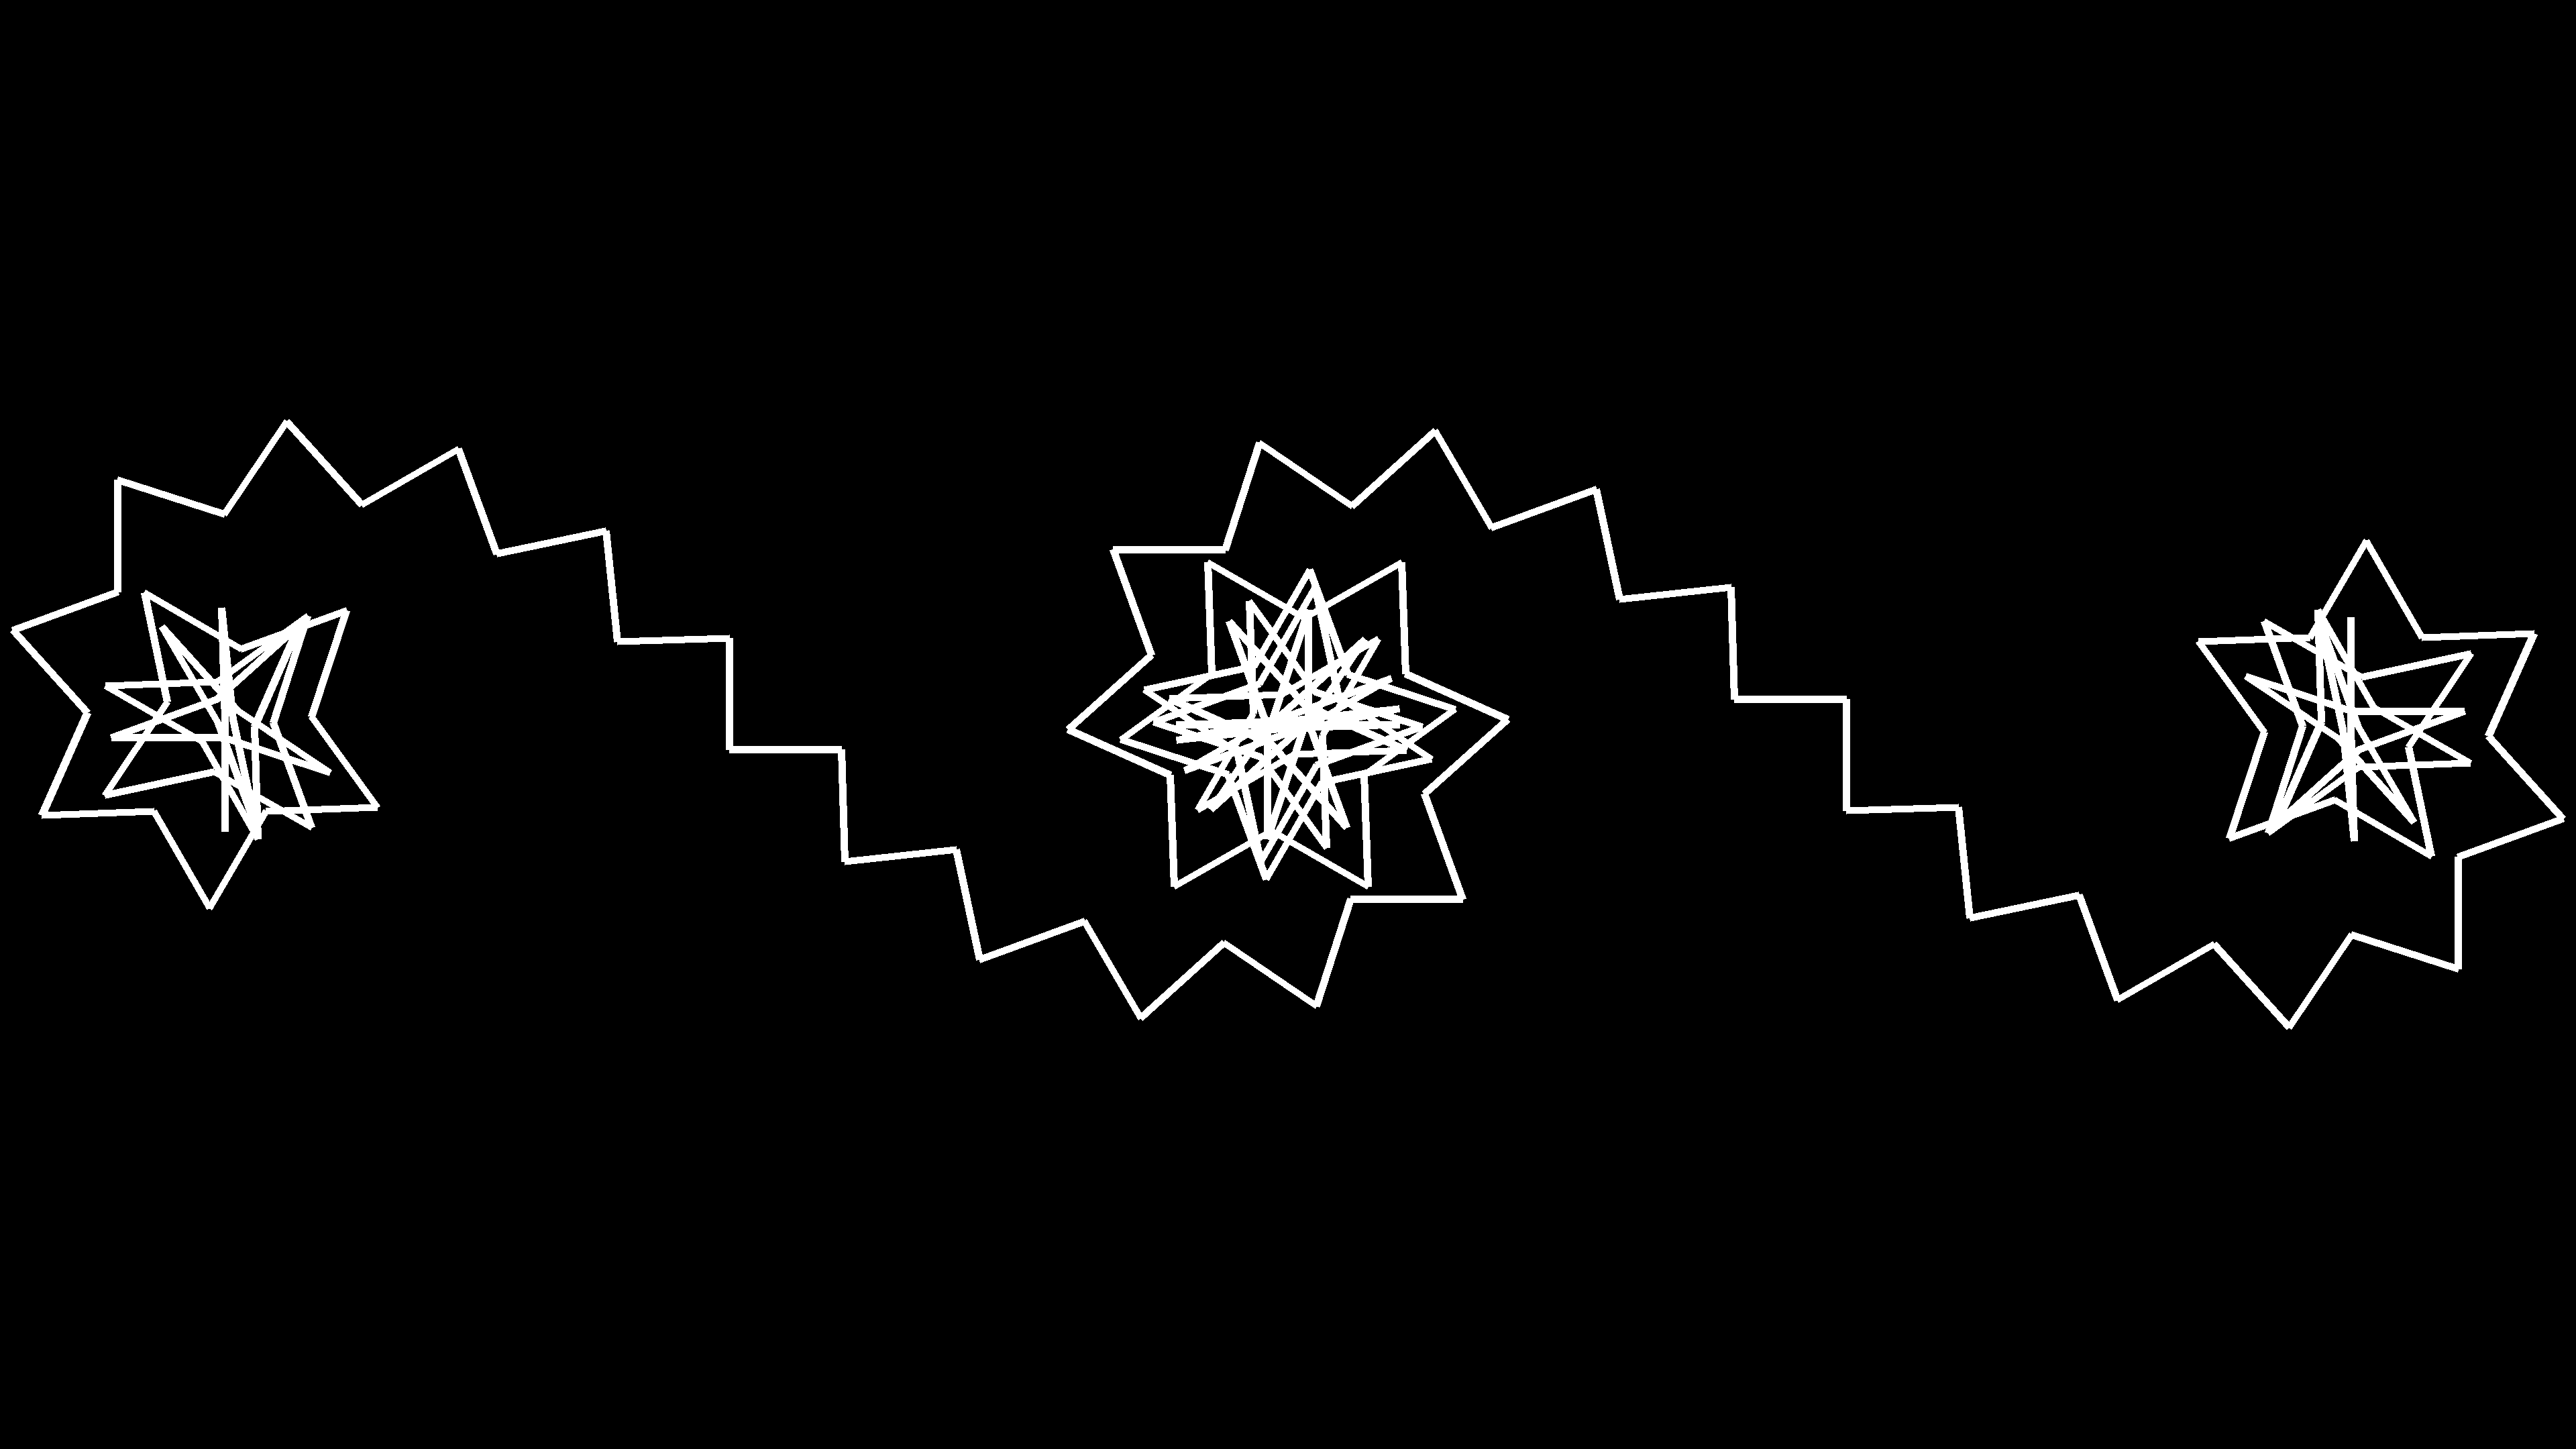
\includegraphics[width=0.3\textwidth]{tf_p=89--q=180--theta=178_00000000.png}
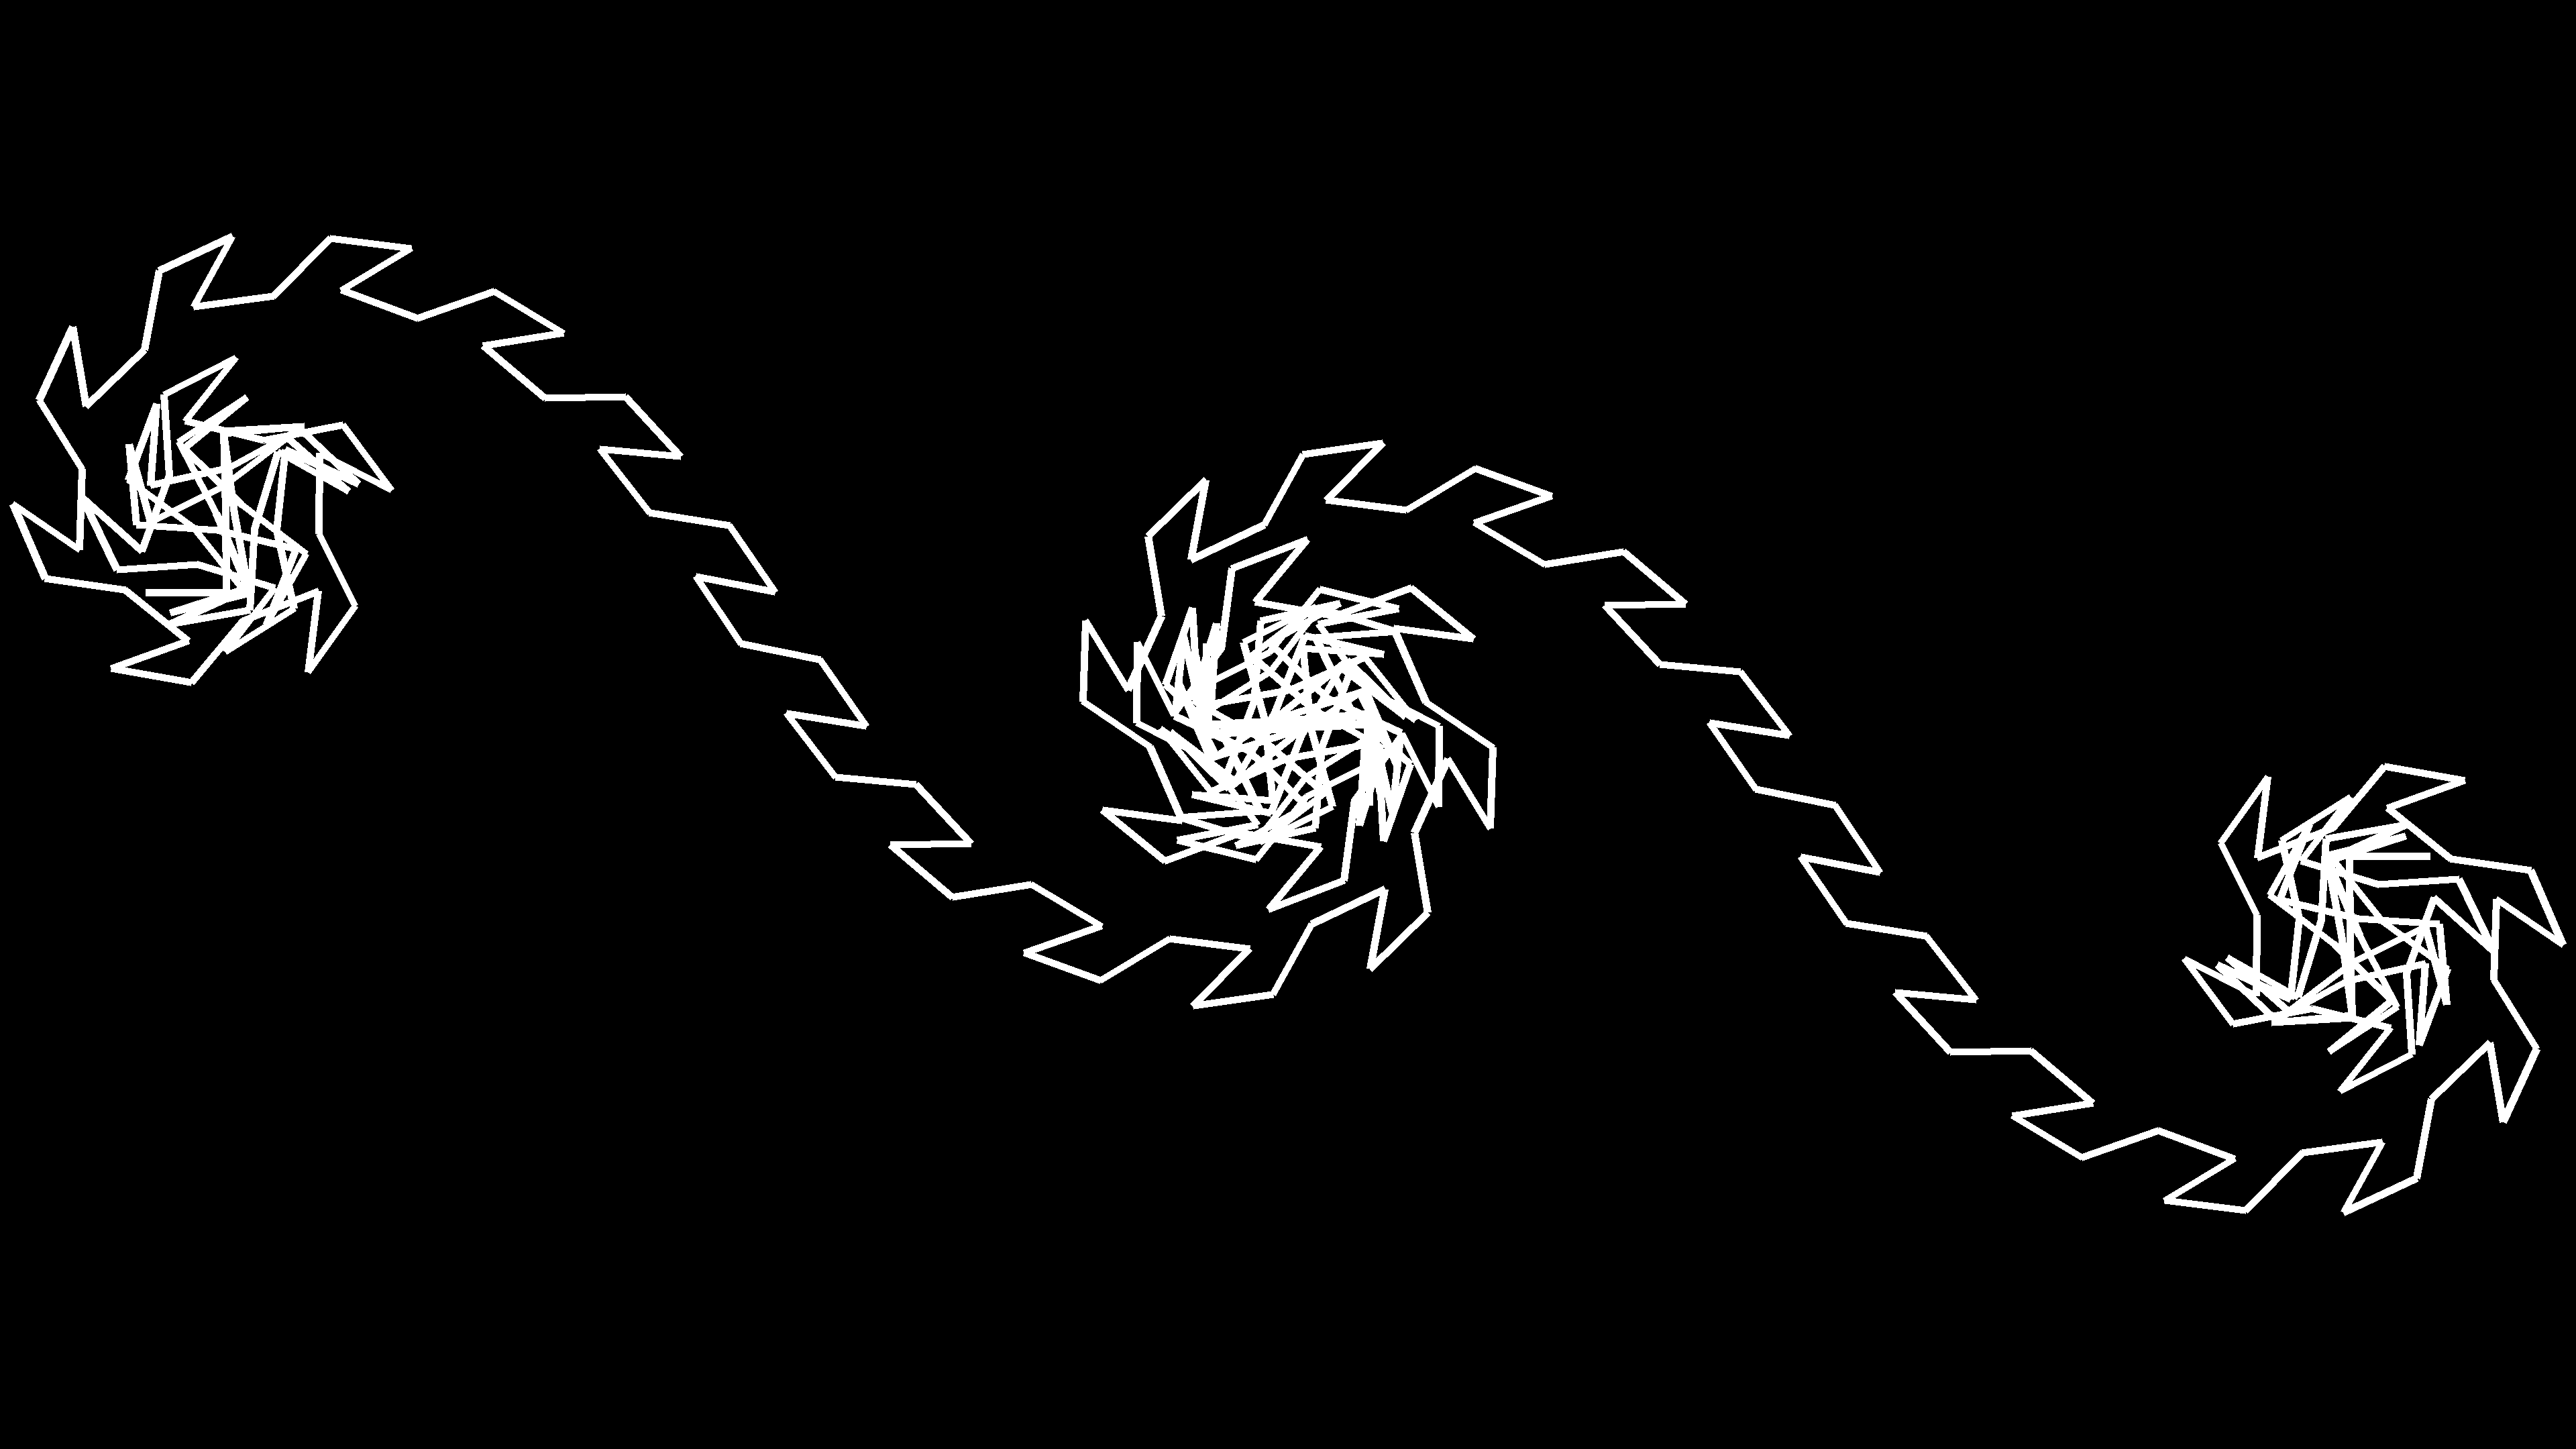
\includegraphics[width=0.3\textwidth]{tf_p=89--q=358--theta=089_49720670.png}


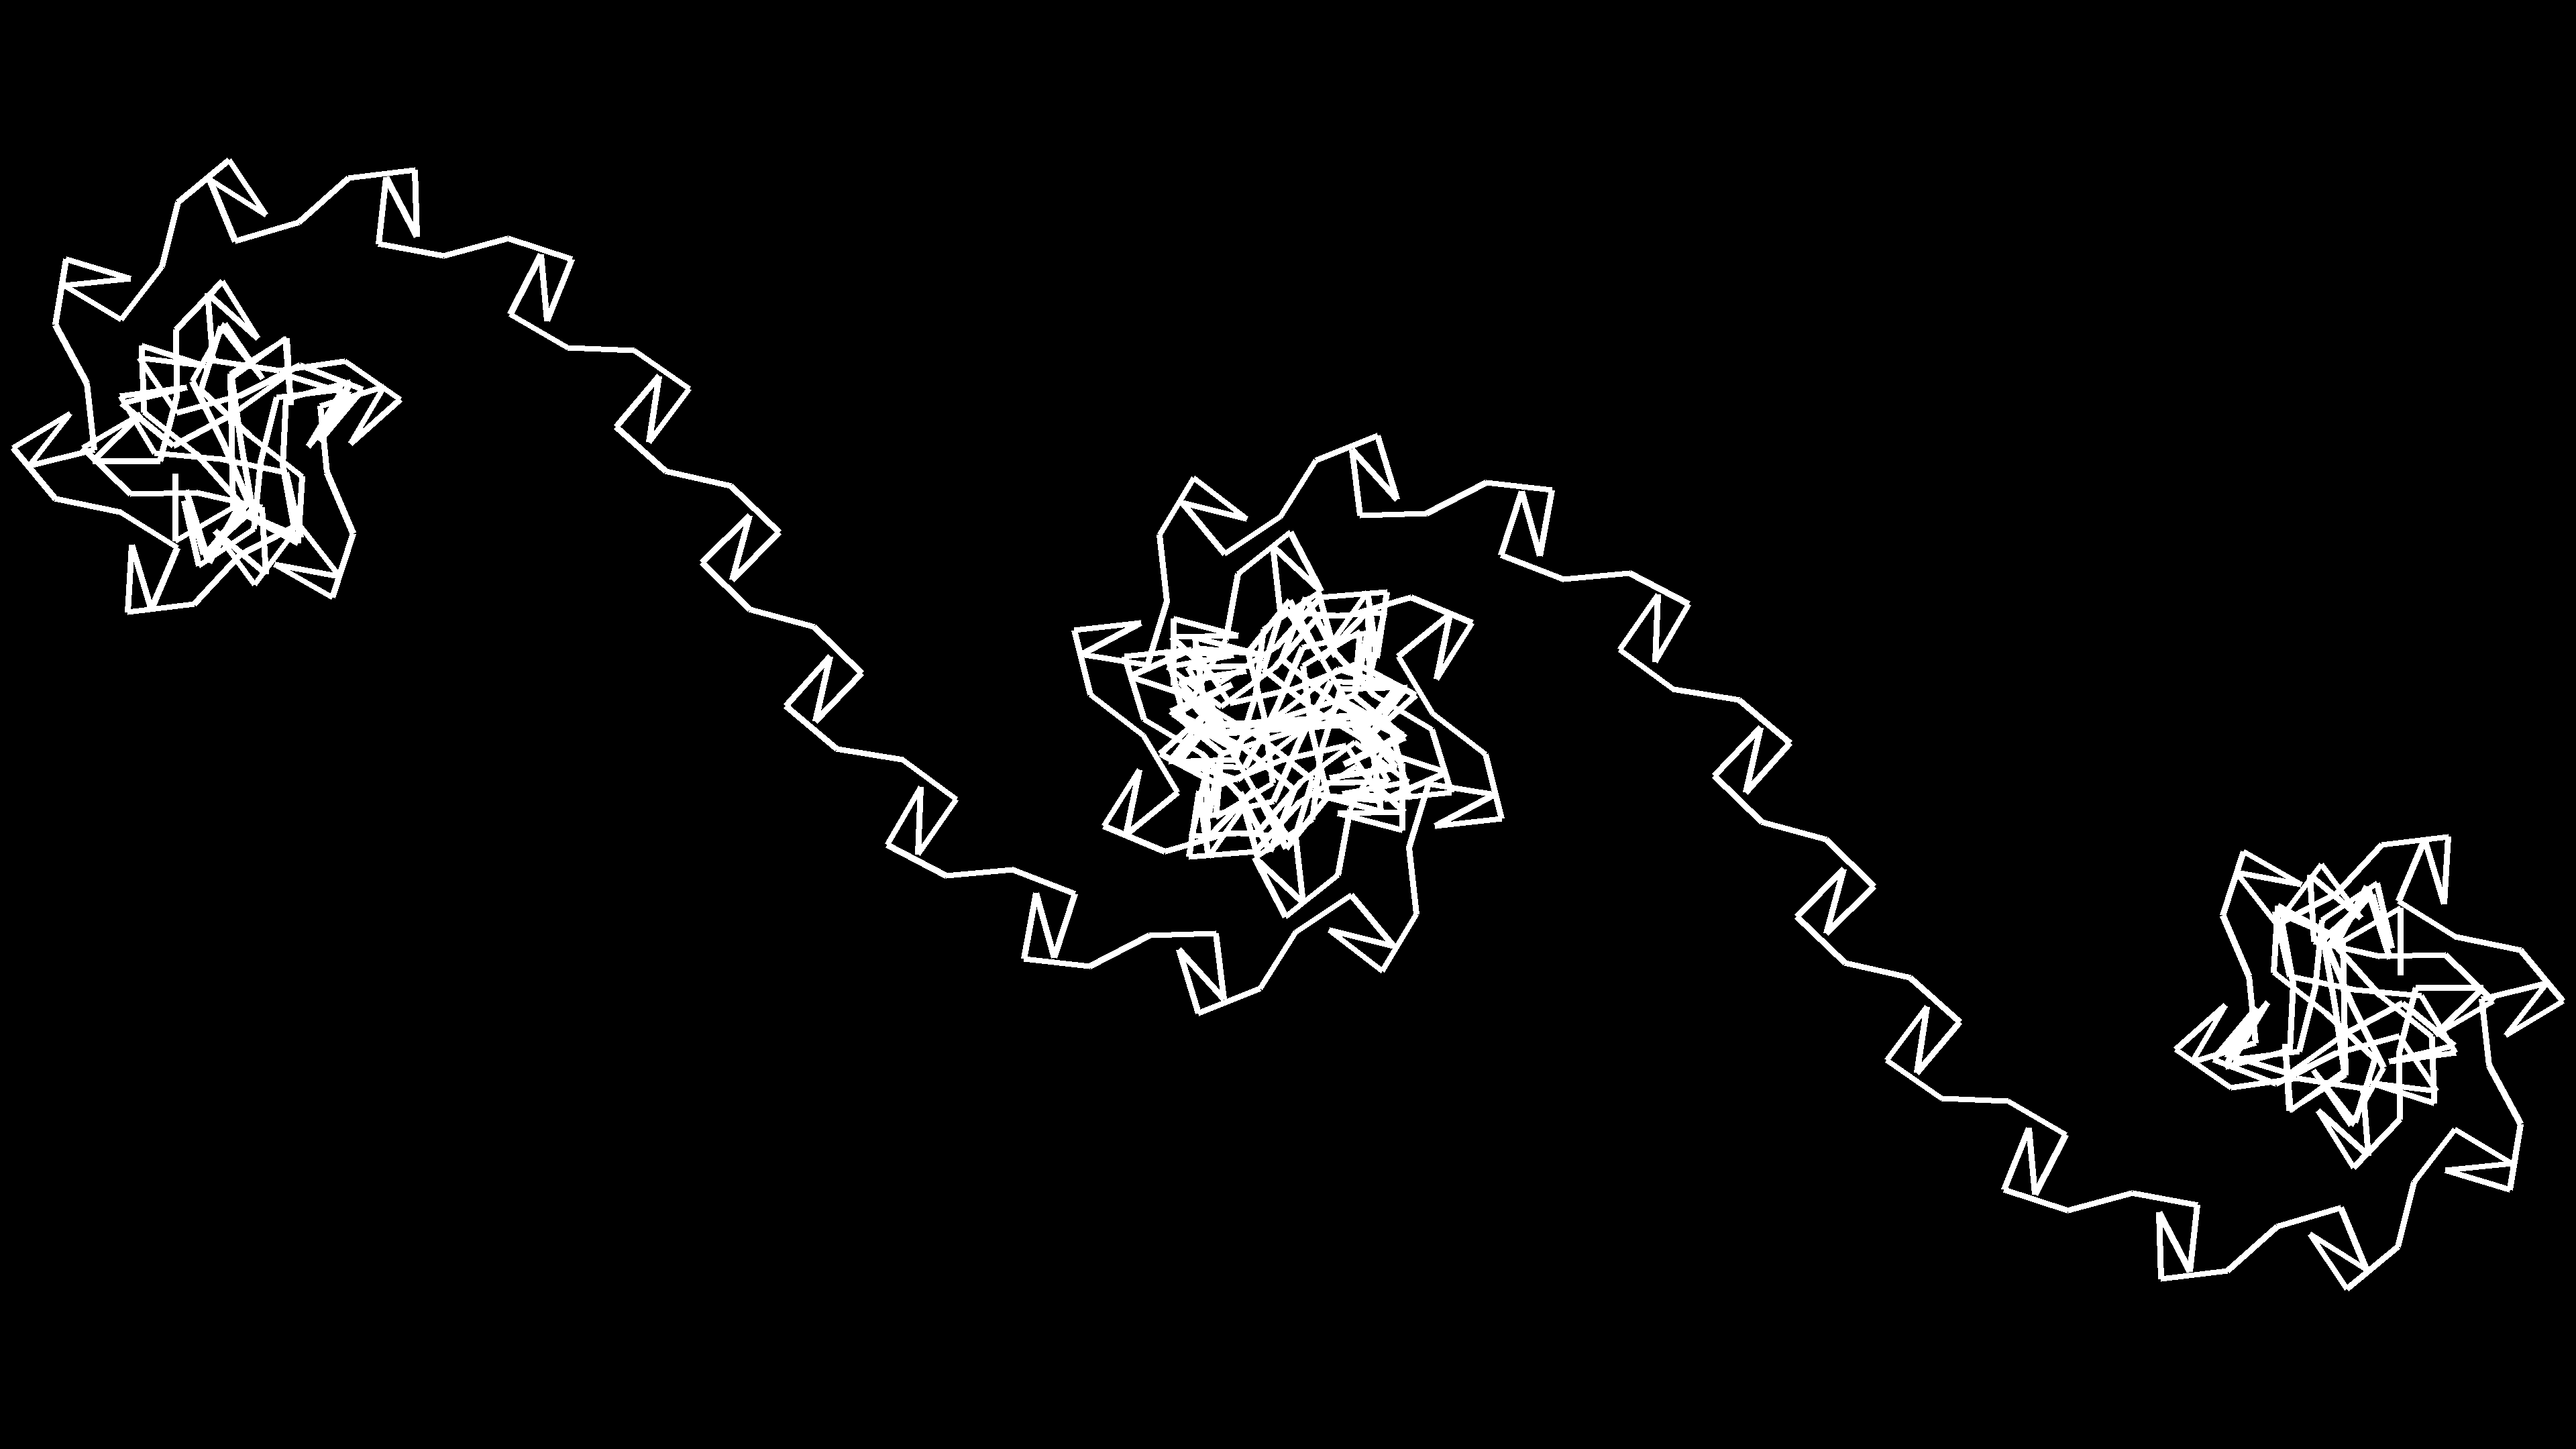
\includegraphics[width=0.3\textwidth]{tf_p=89--q=536--theta=059_77611940.png}
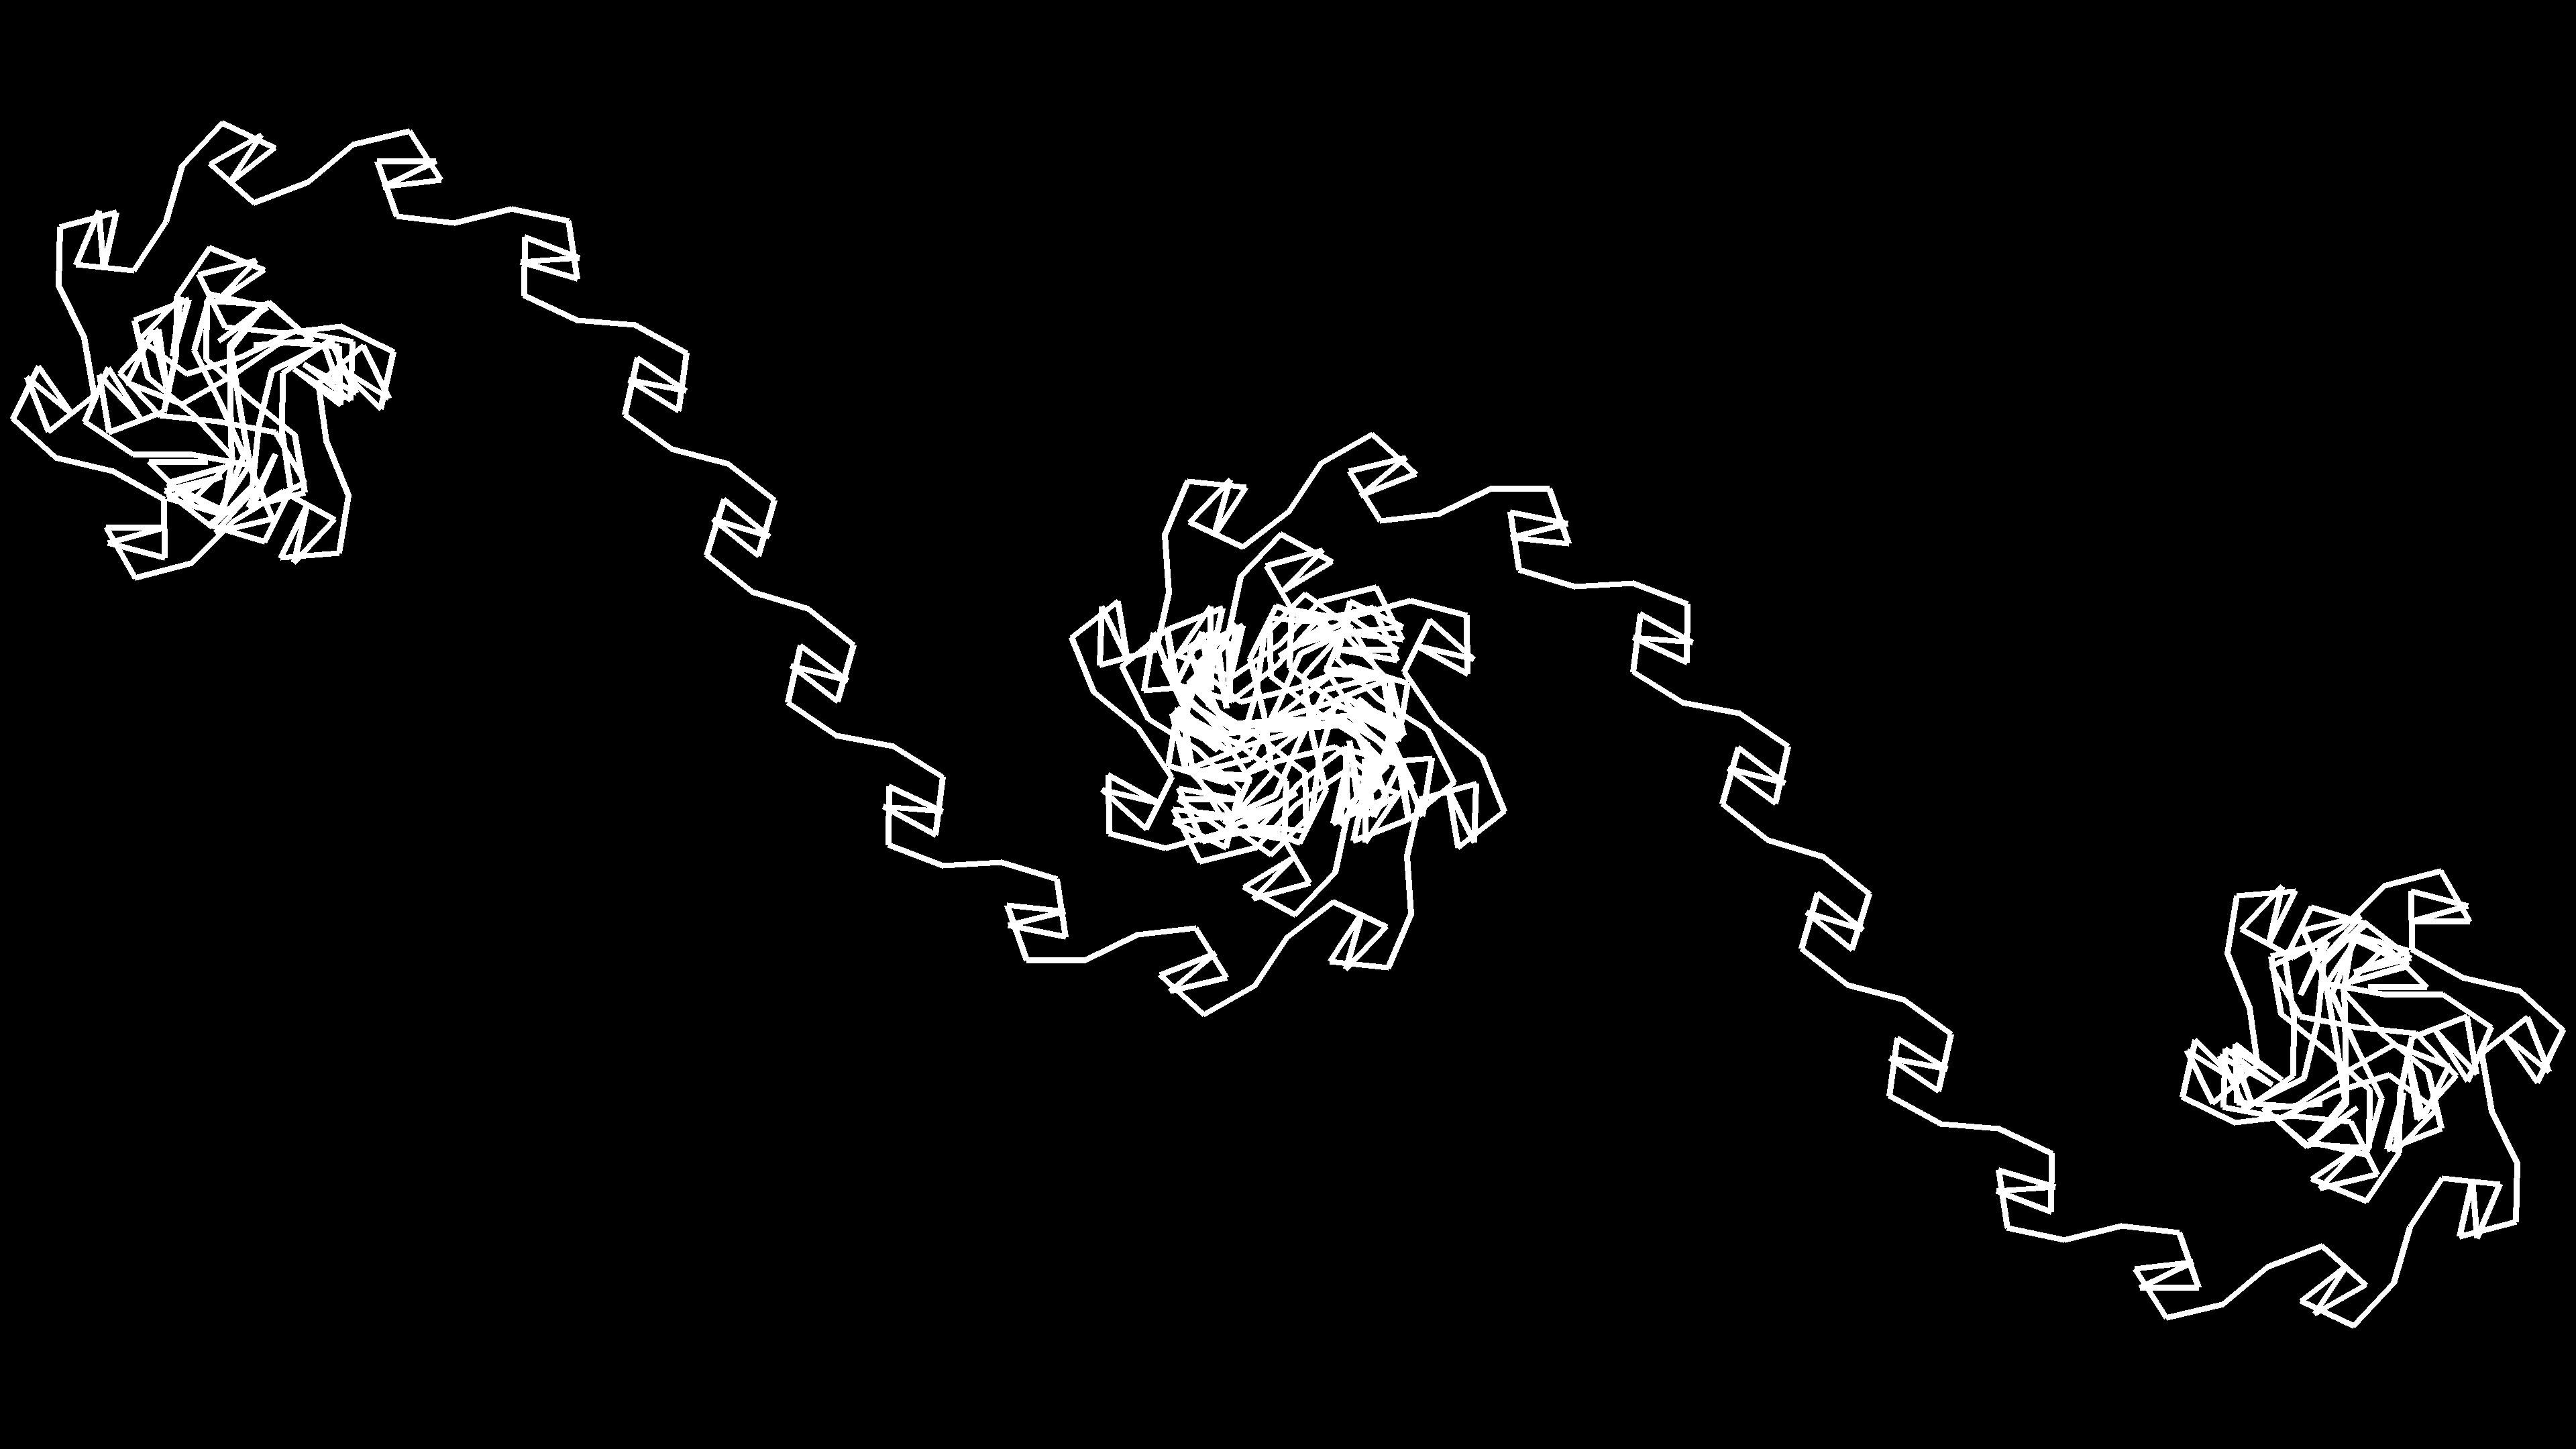
\includegraphics[width=0.3\textwidth]{tf_p=89--q=714--theta=044_87394958.png}
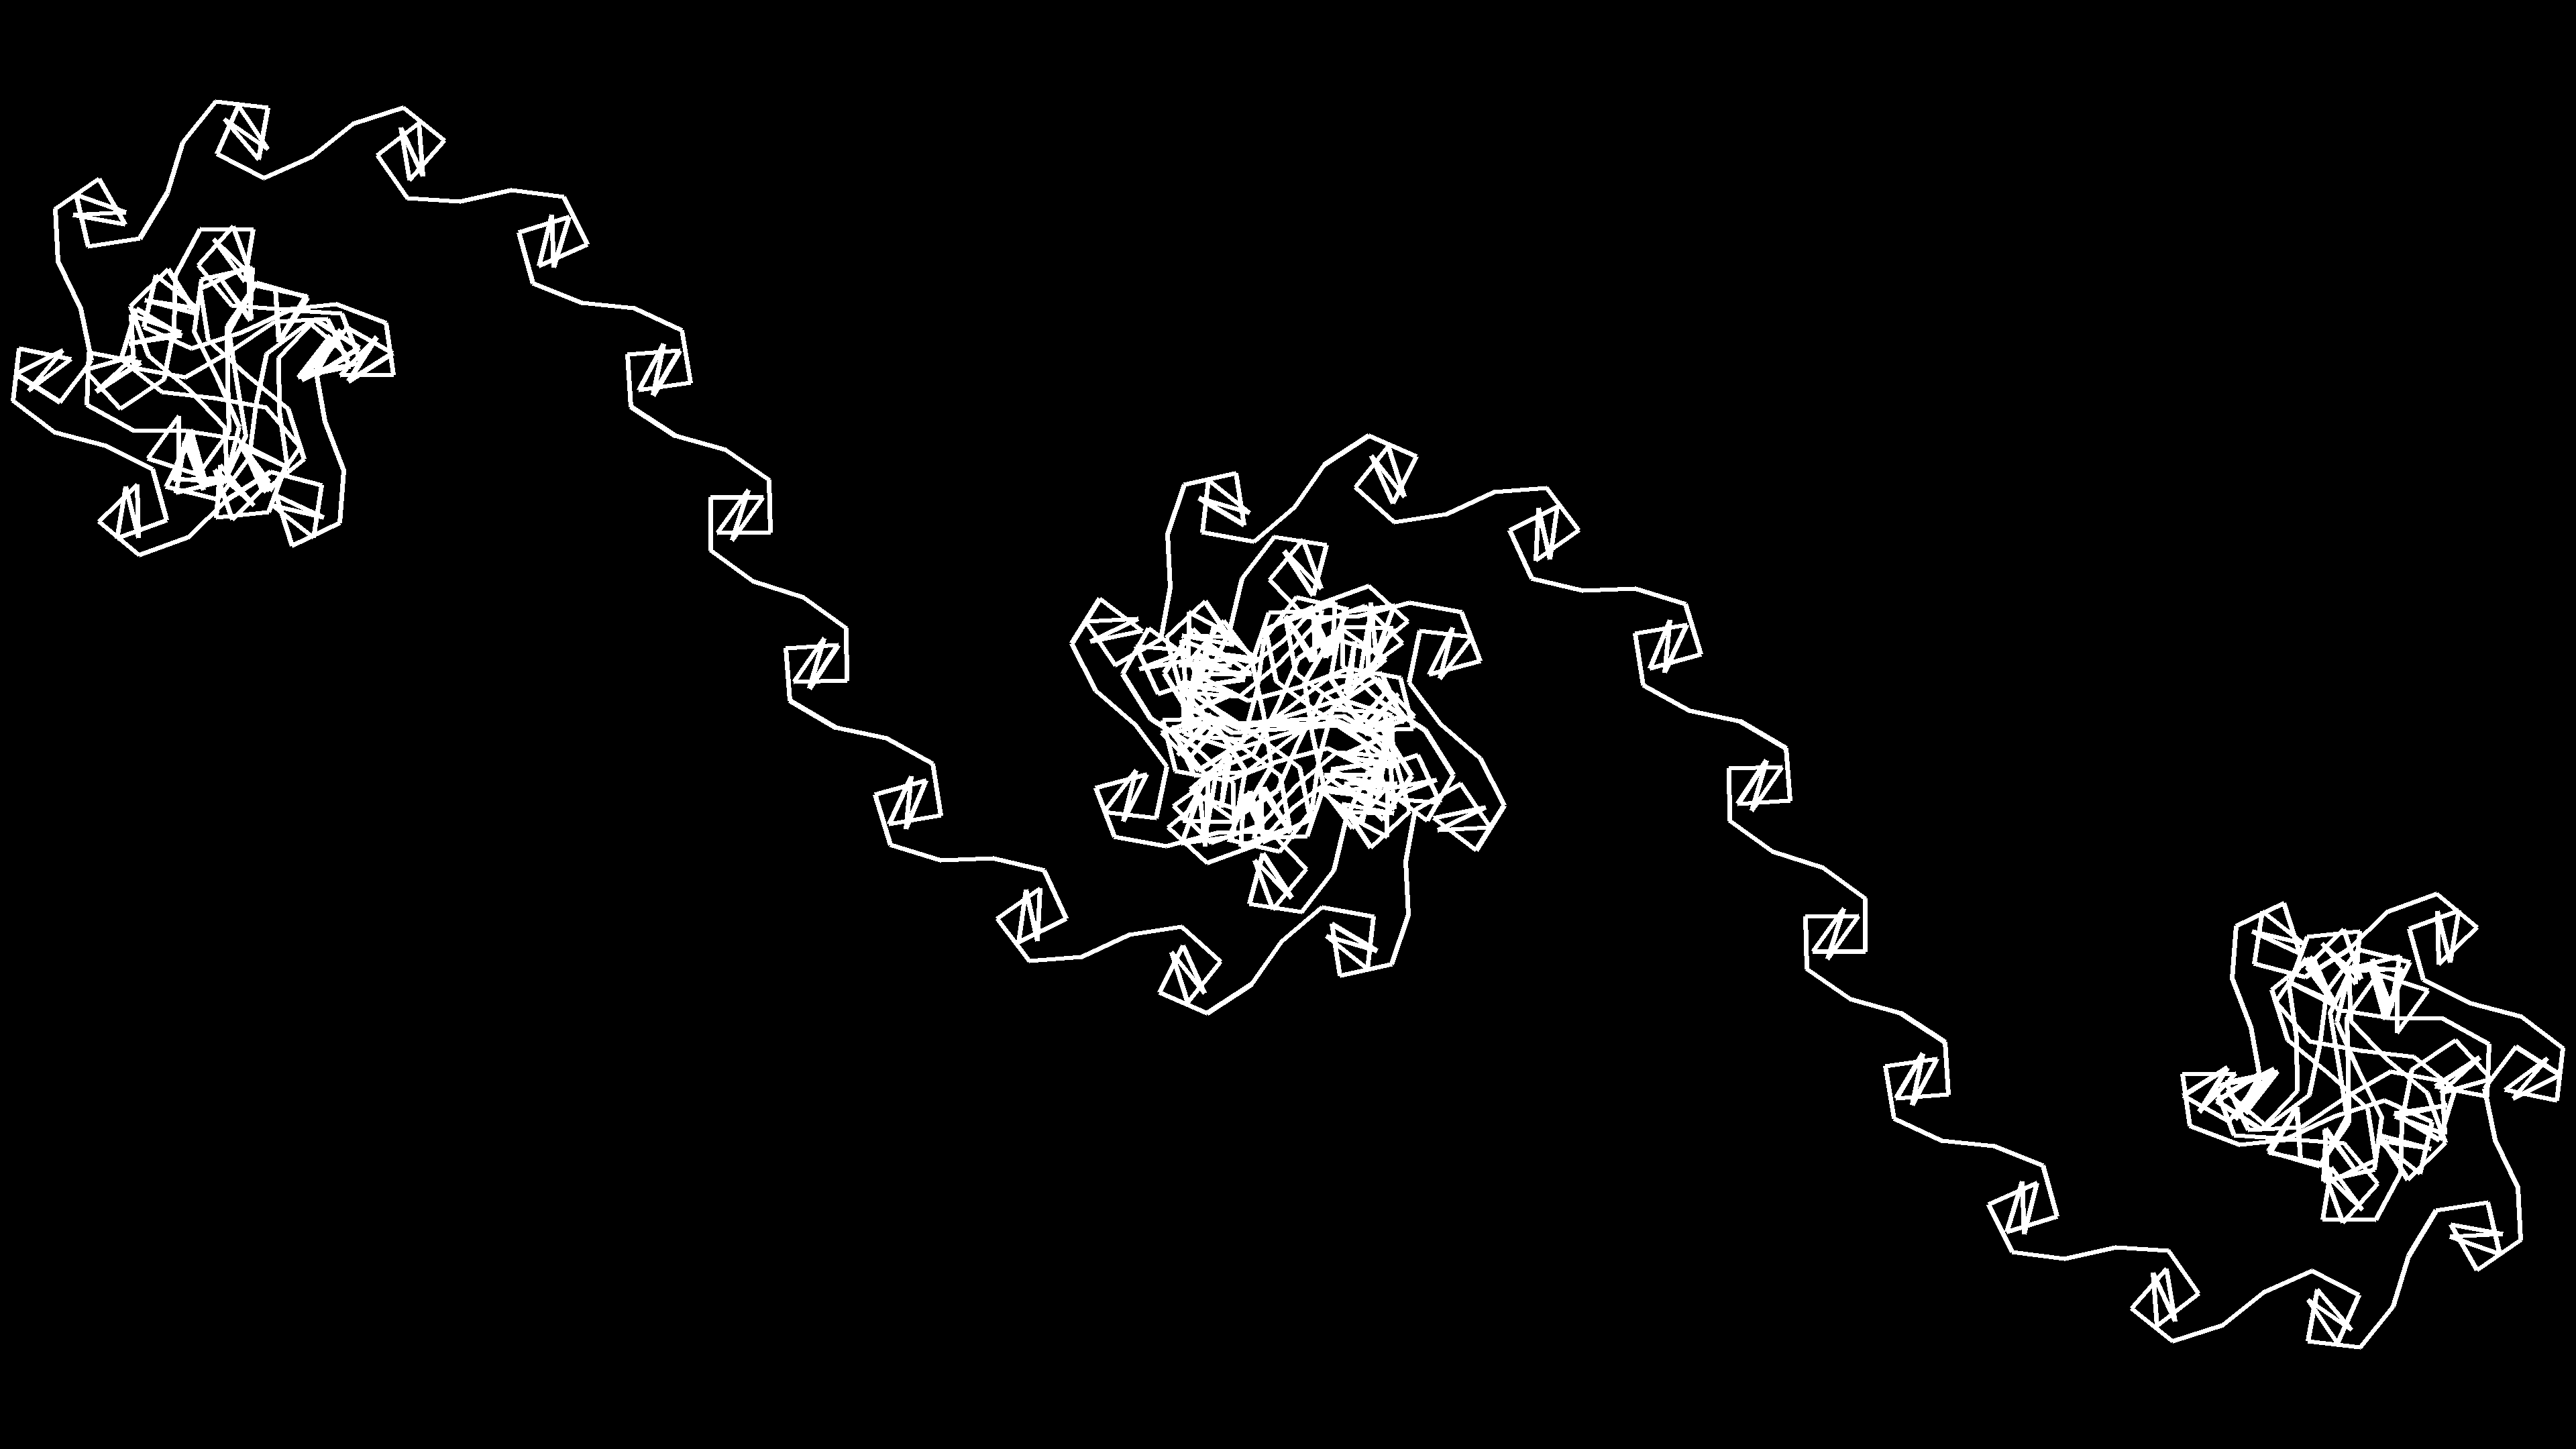
\includegraphics[width=0.3\textwidth]{tf_p=89--q=892--theta=035_91928251.png}


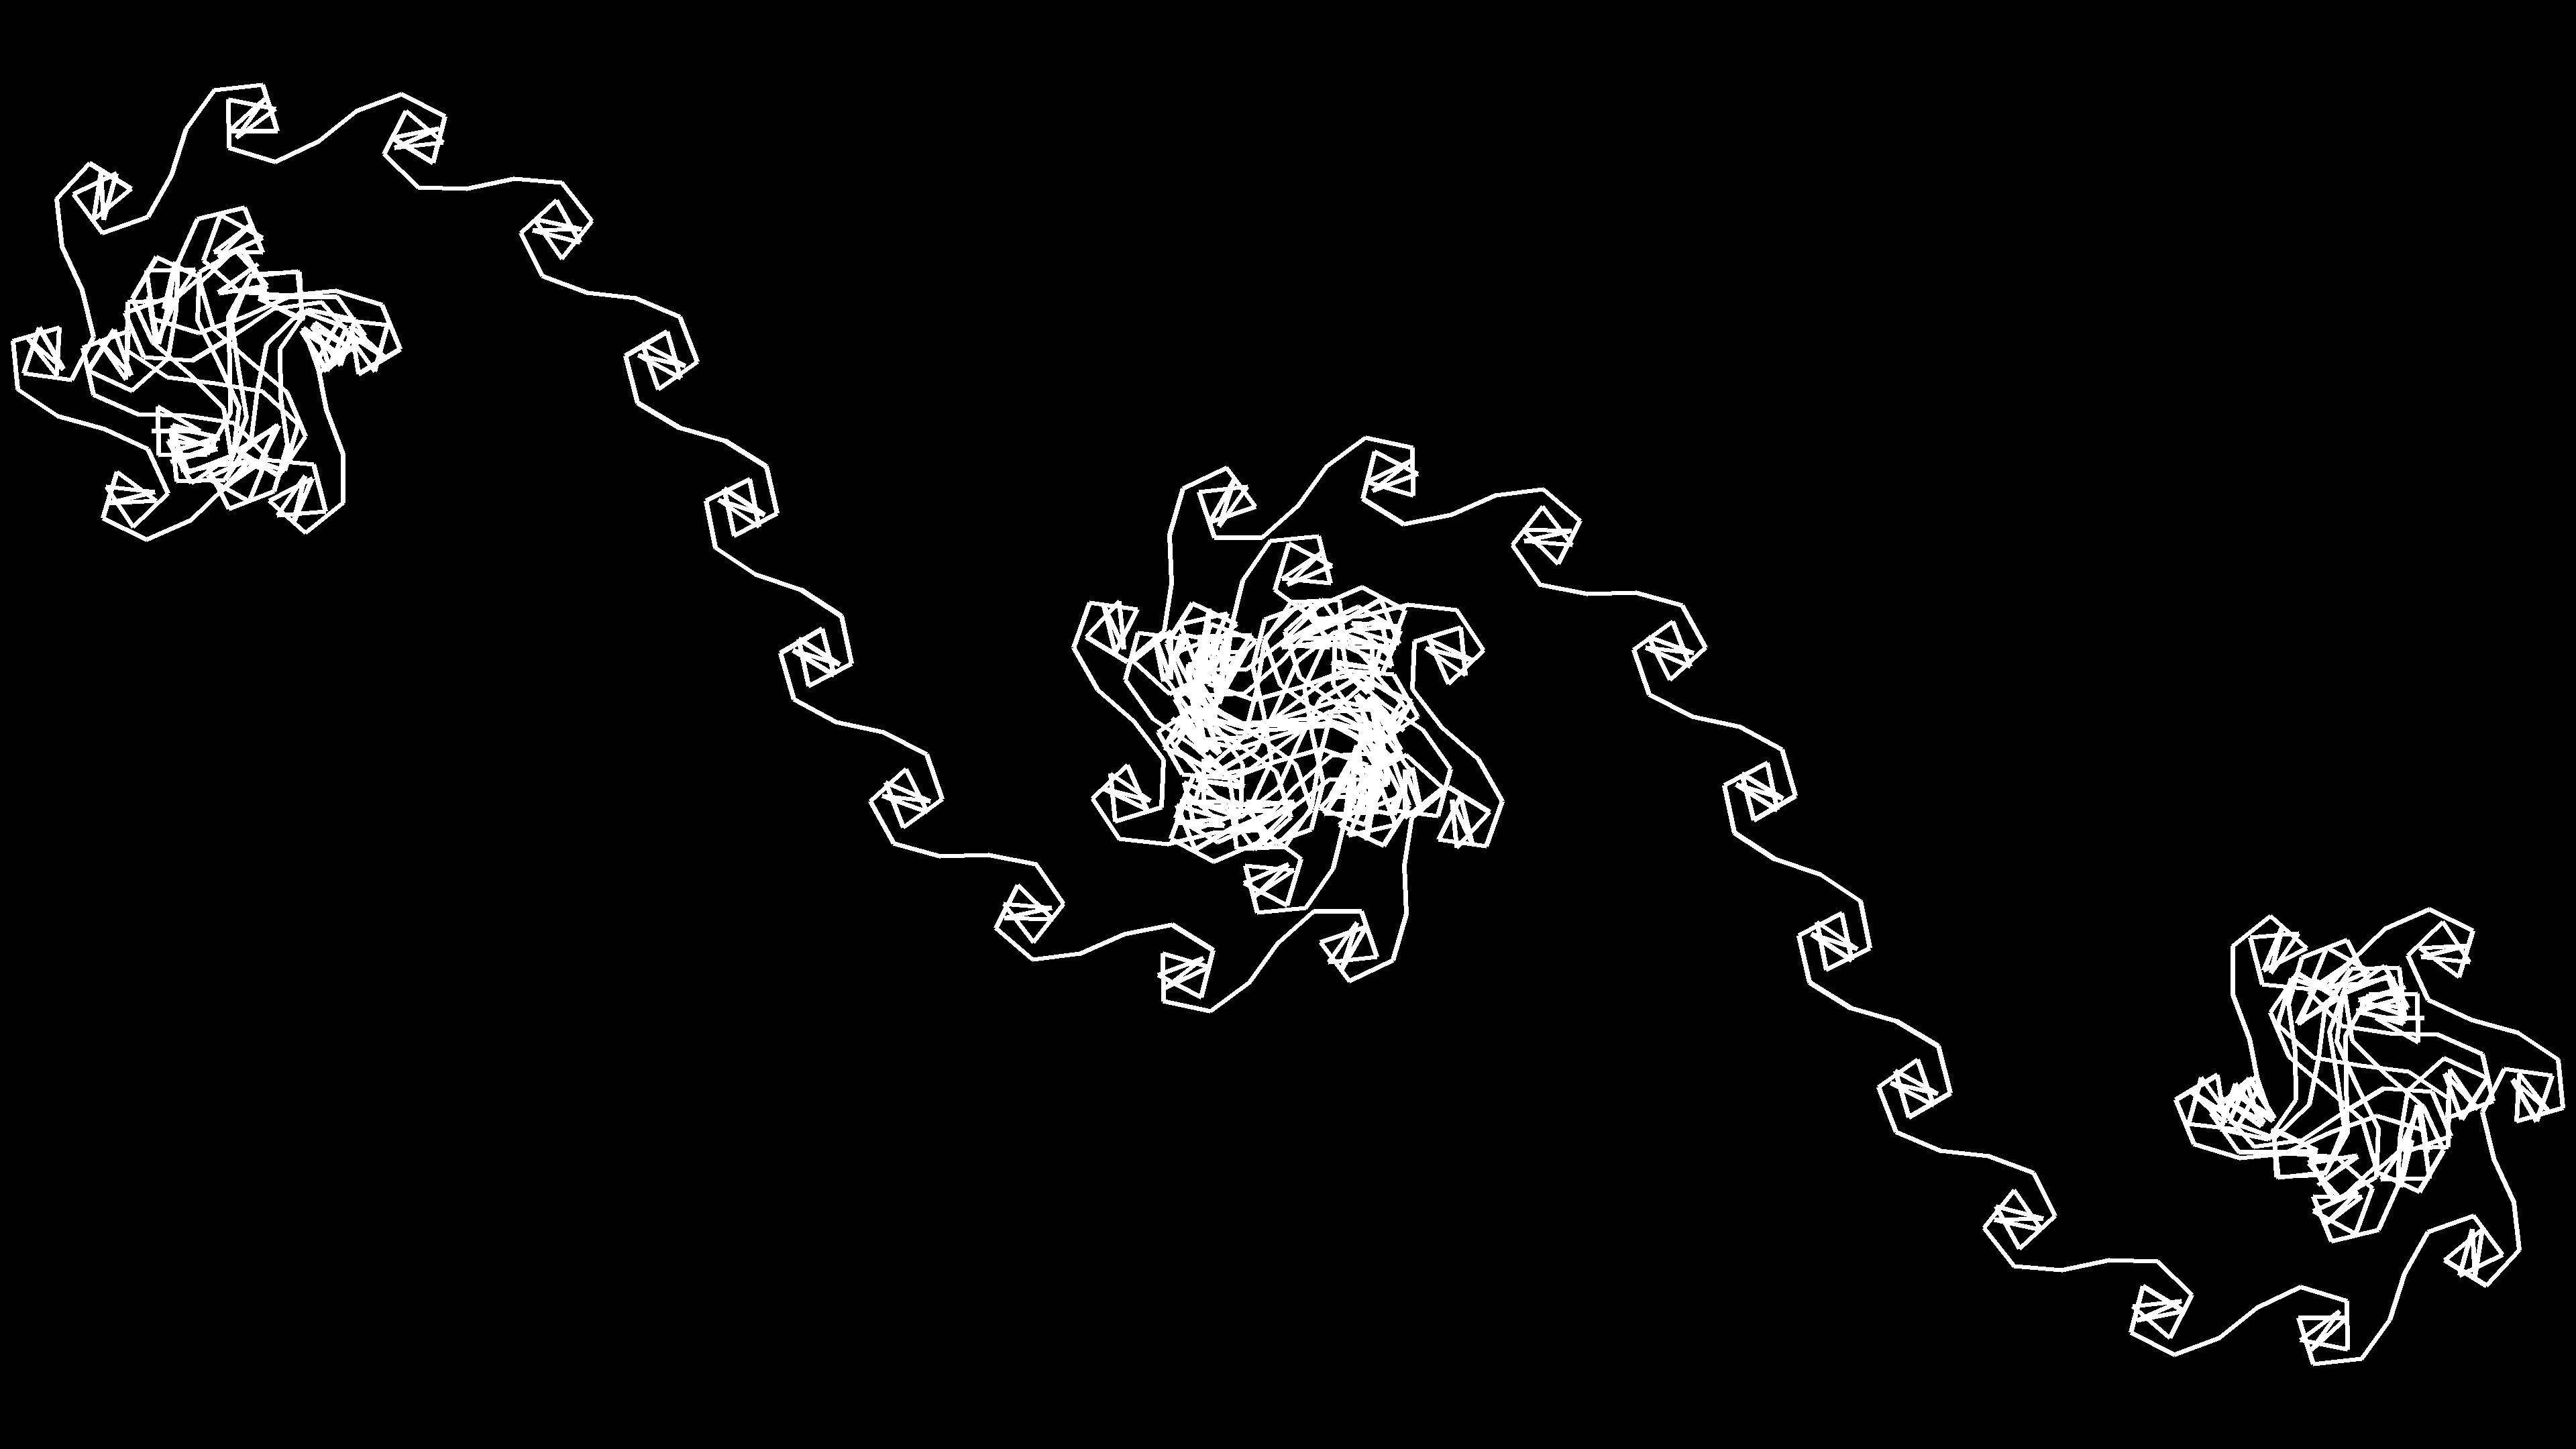
\includegraphics[width=0.3\textwidth]{tf_p=89--q=1070--theta=029_94392523.png}
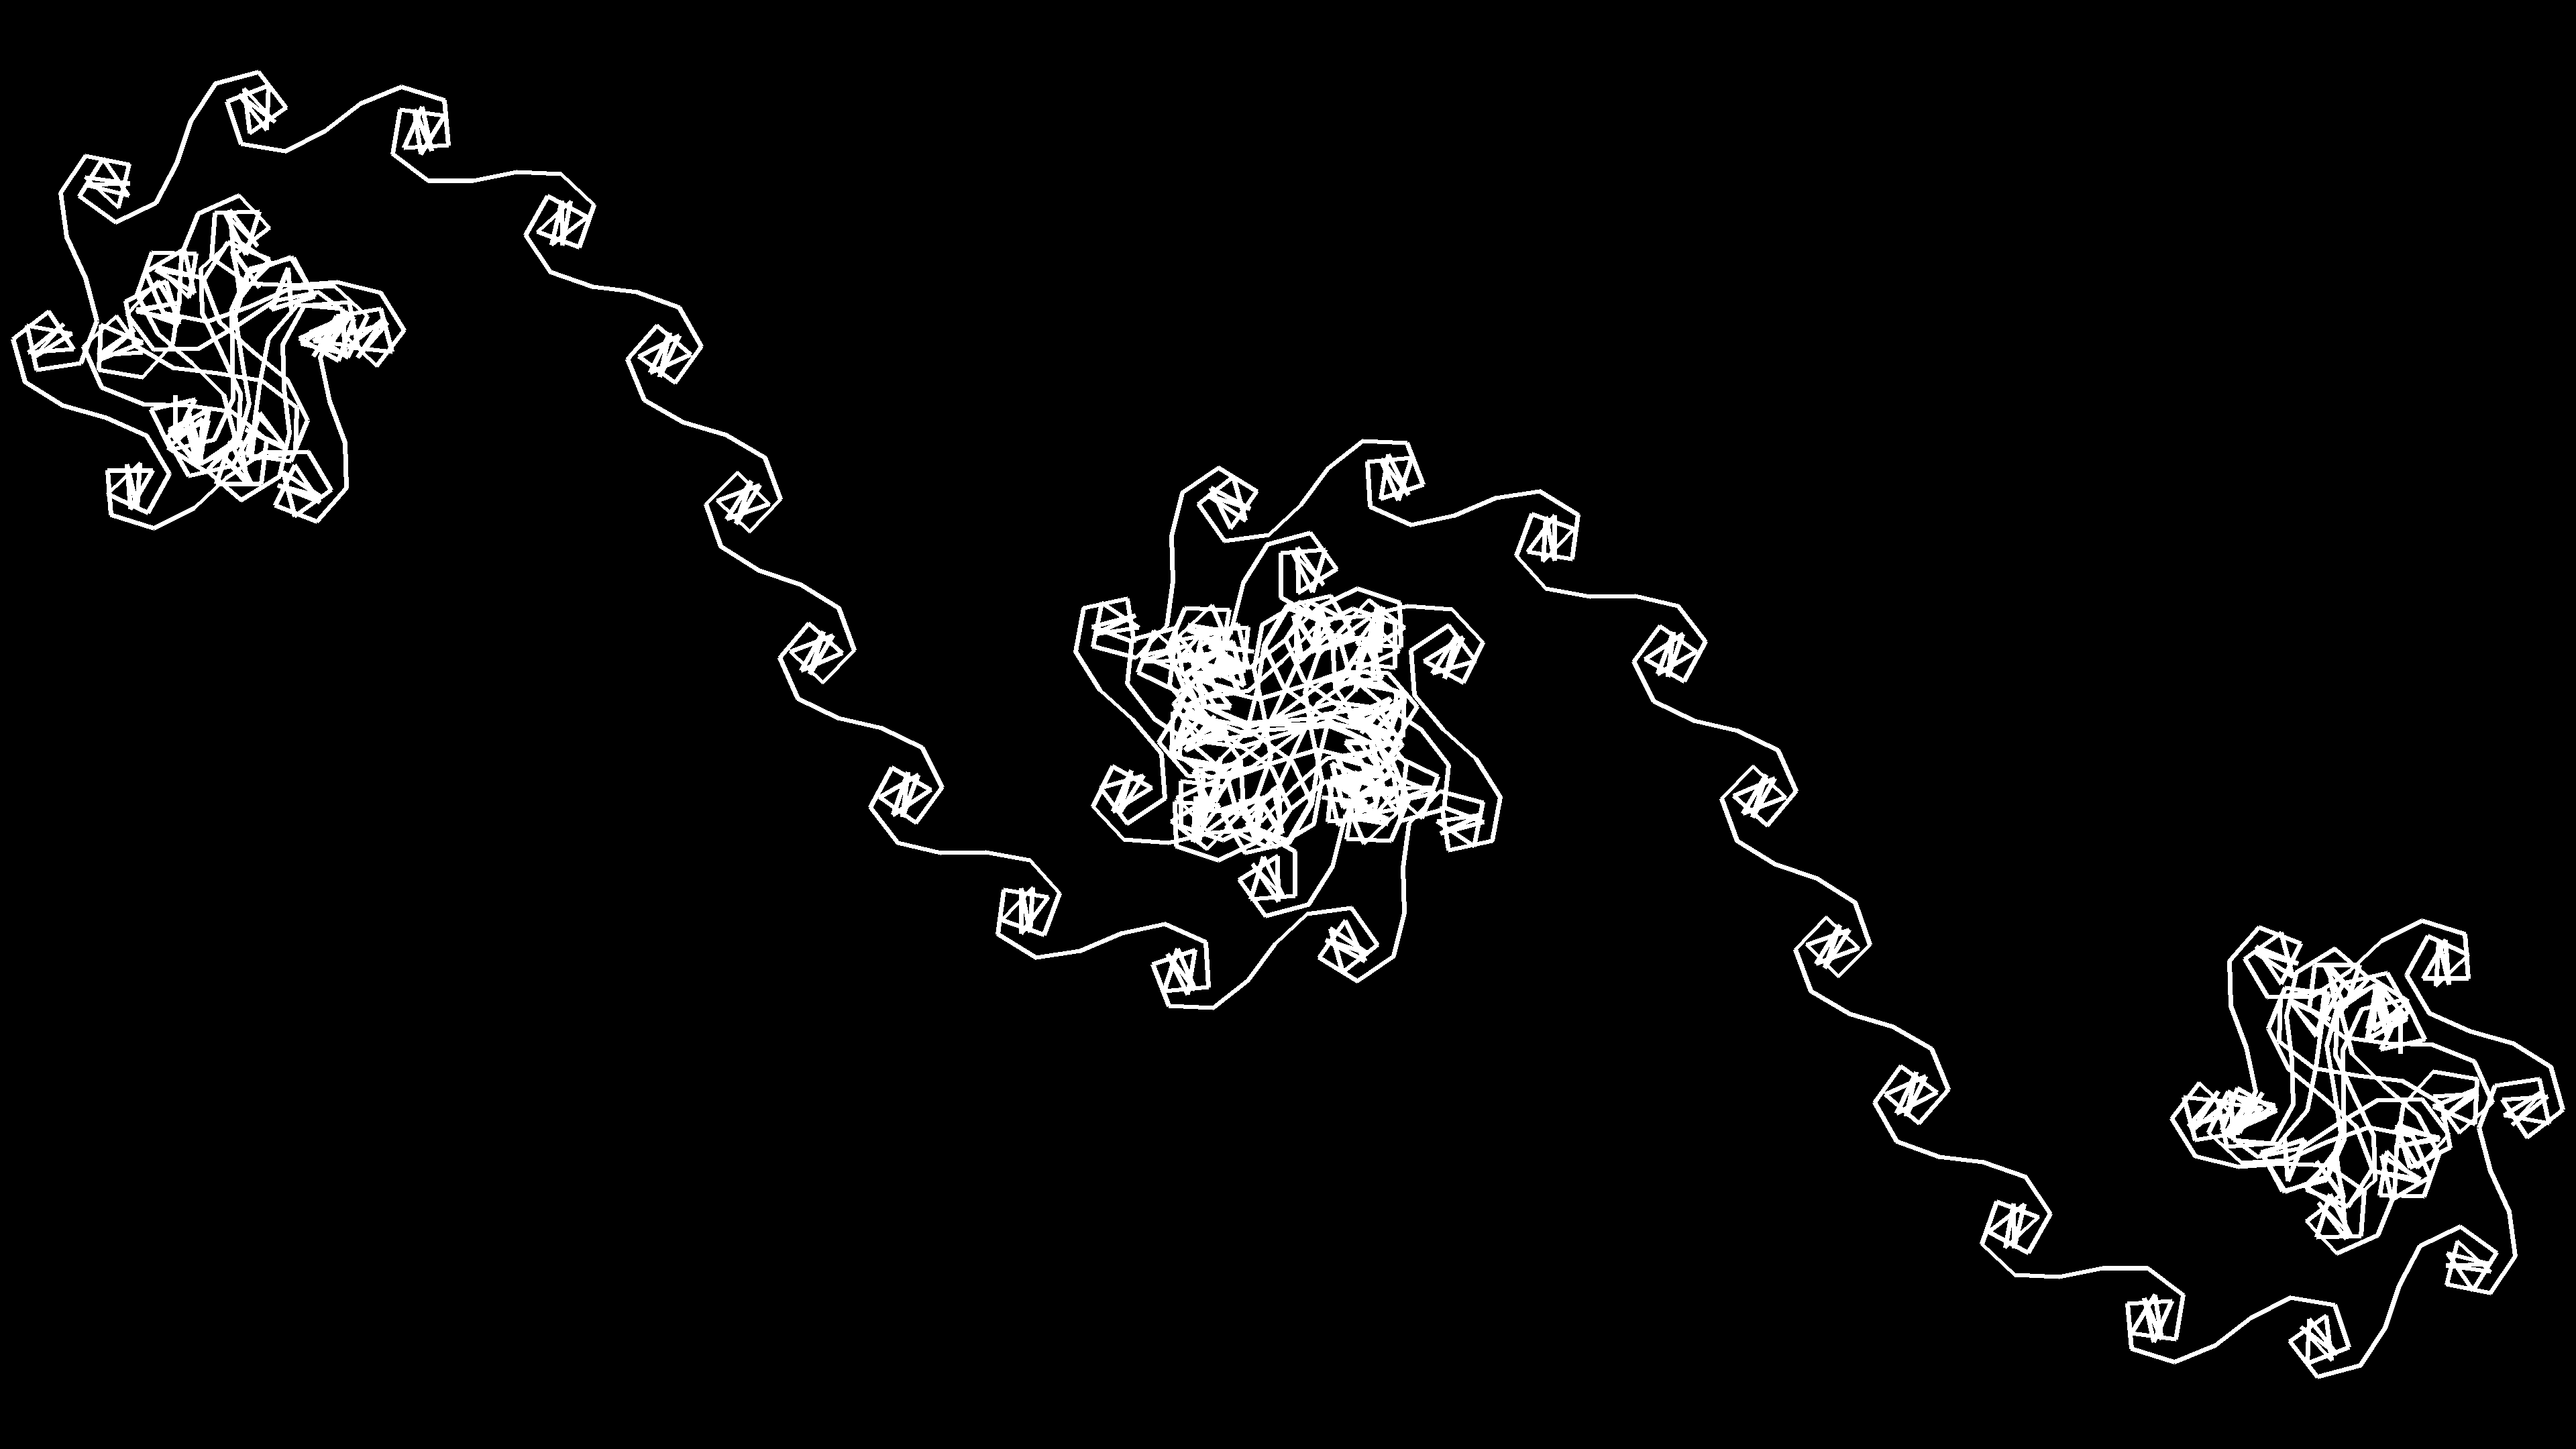
\includegraphics[width=0.3\textwidth]{tf_p=89--q=1248--theta=025_67307692.png}
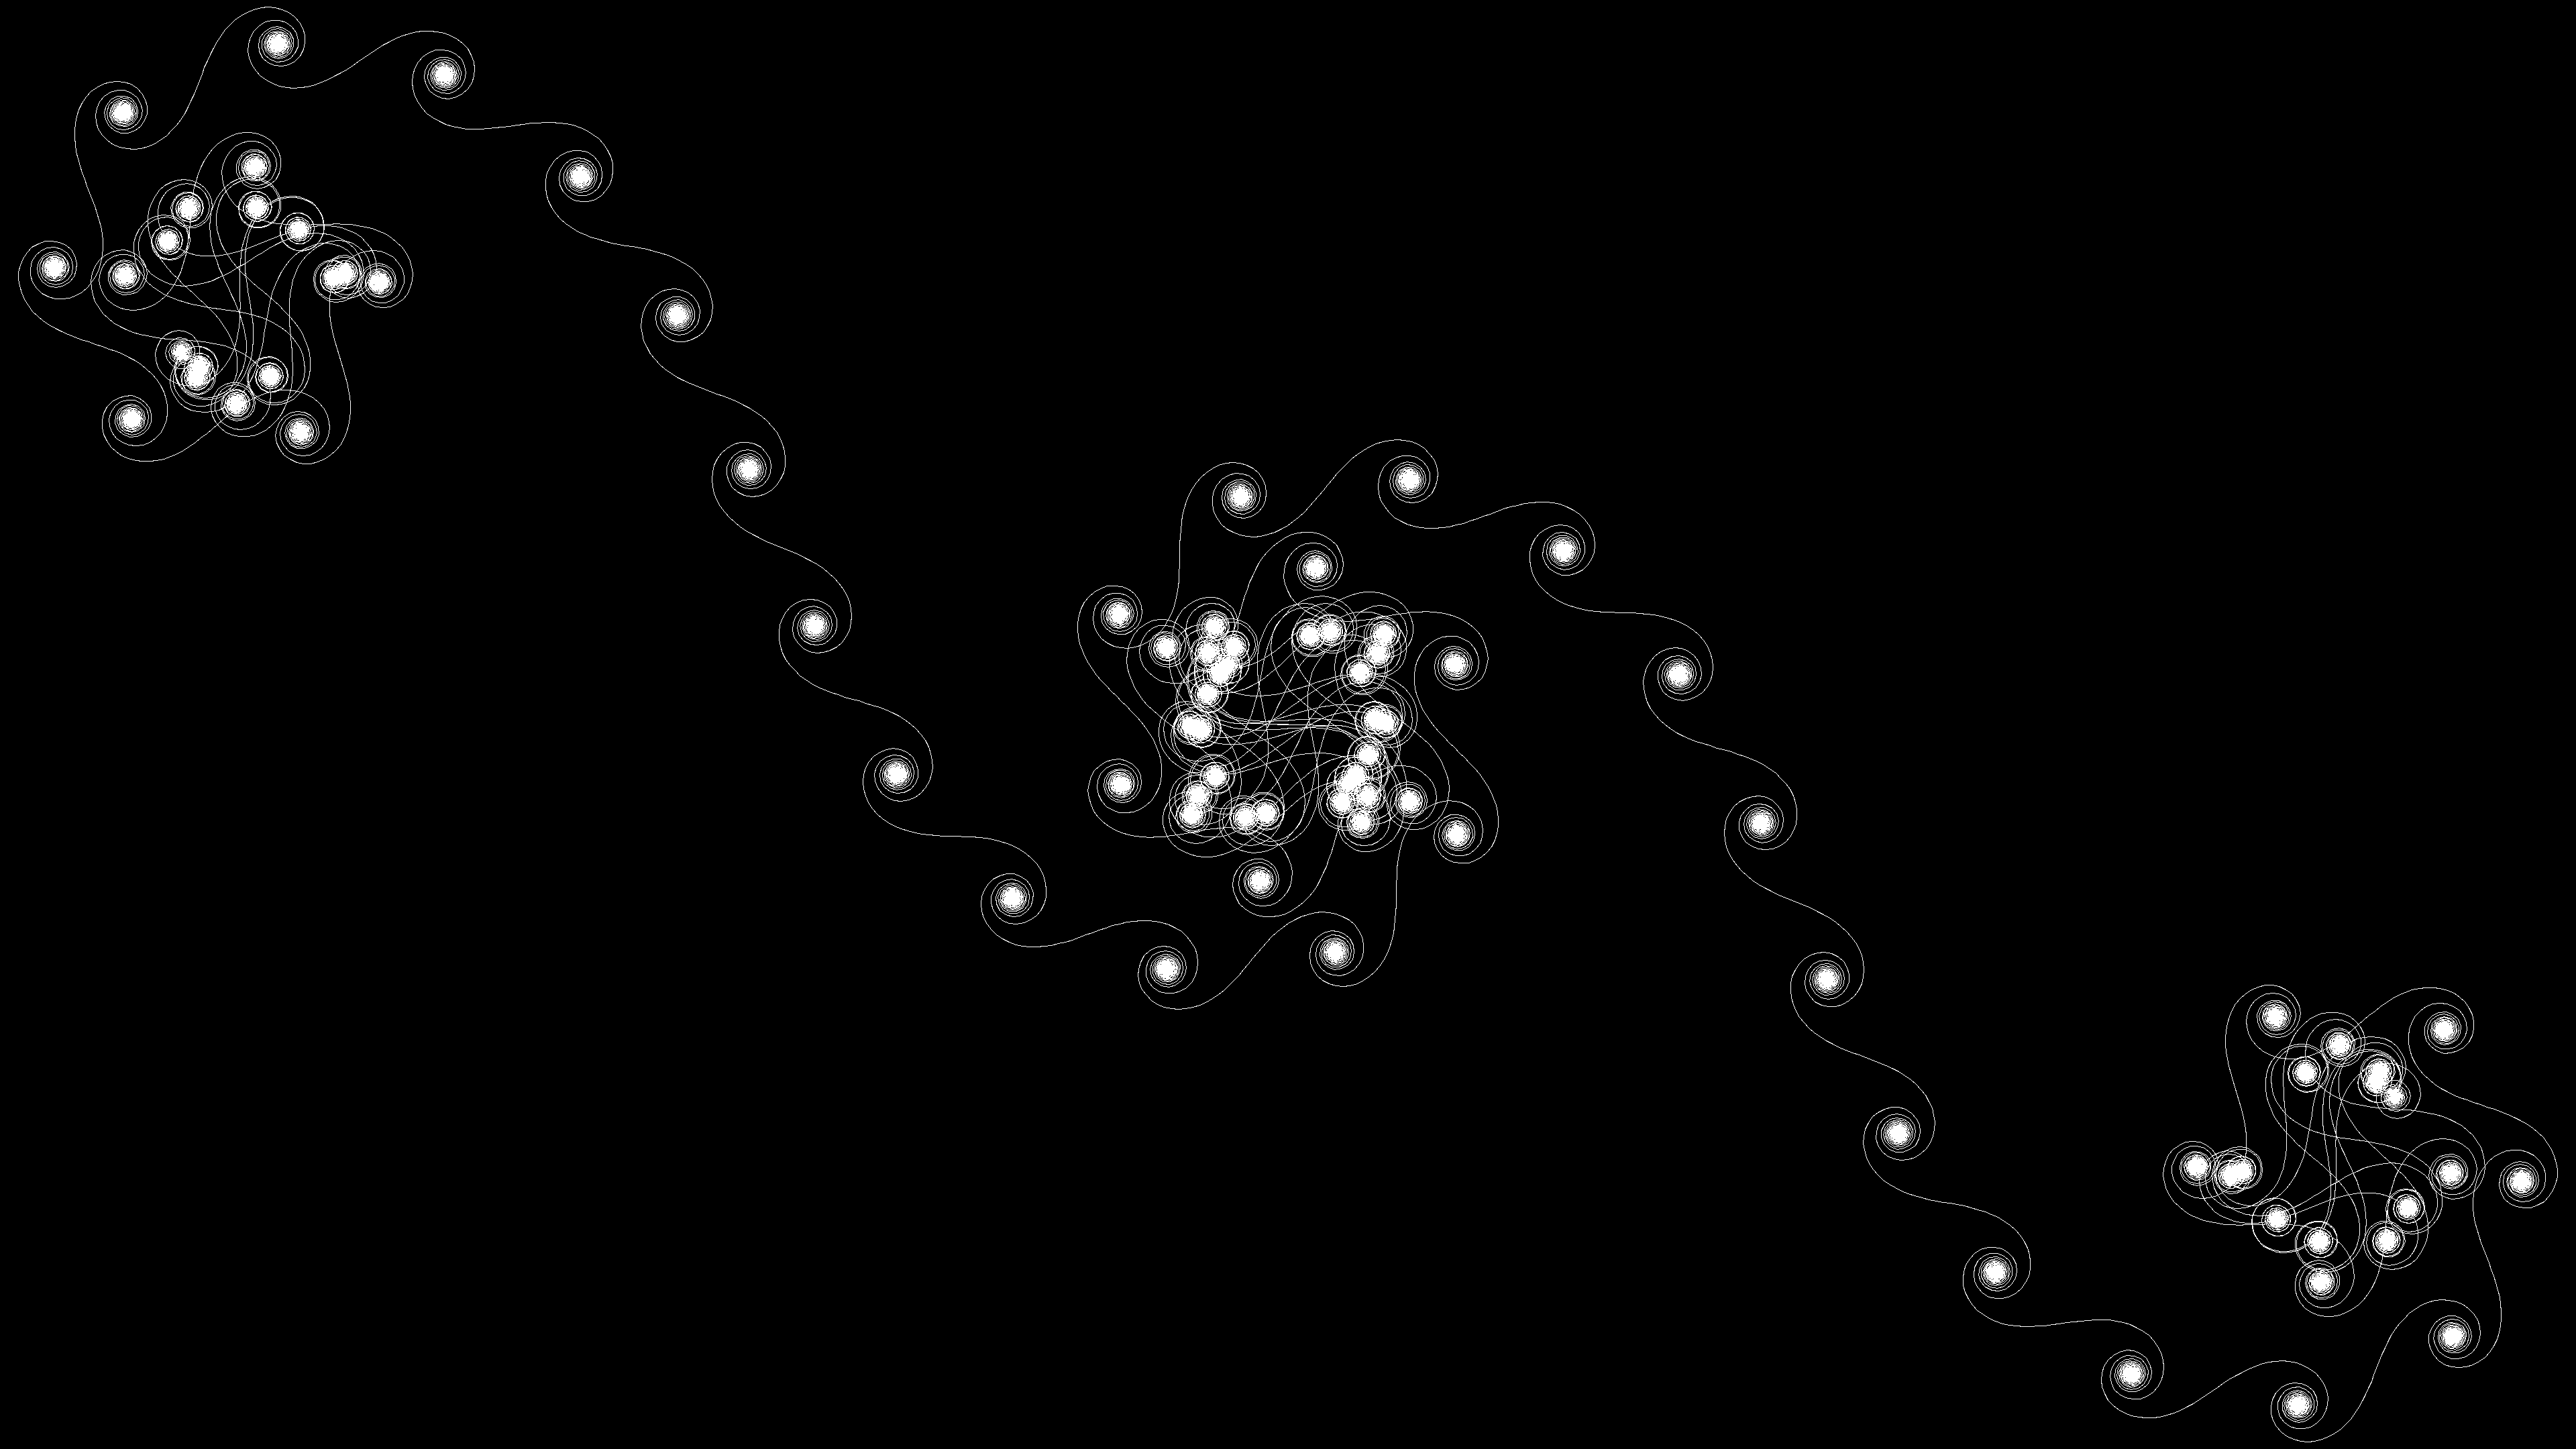
\includegraphics[width=0.3\textwidth]{tf_p=89--q=49842--theta=000_64283135.png}

It can be observed, that the image rotates slowly into it's final position, as the exit angles out of the individual
Euler Spirals get more and more defined.

If an Euler spiral is defined as the connection between two 'circles', the number of Euler spirals is equal to $p$ for
any given image.

Within the $p, q$ space there are two very stable images: the horizontal and the vertical Euler spiral of Euler spirals.
The horizontal ones are created by $q = p \cdot 501 + 1$ and the vertical ones by $q = p \cdot 501 - 1$.

The following image series shows the images for $p \in \{5, 9, 13, 19, 25, 31, 37, 43, 249\}$.

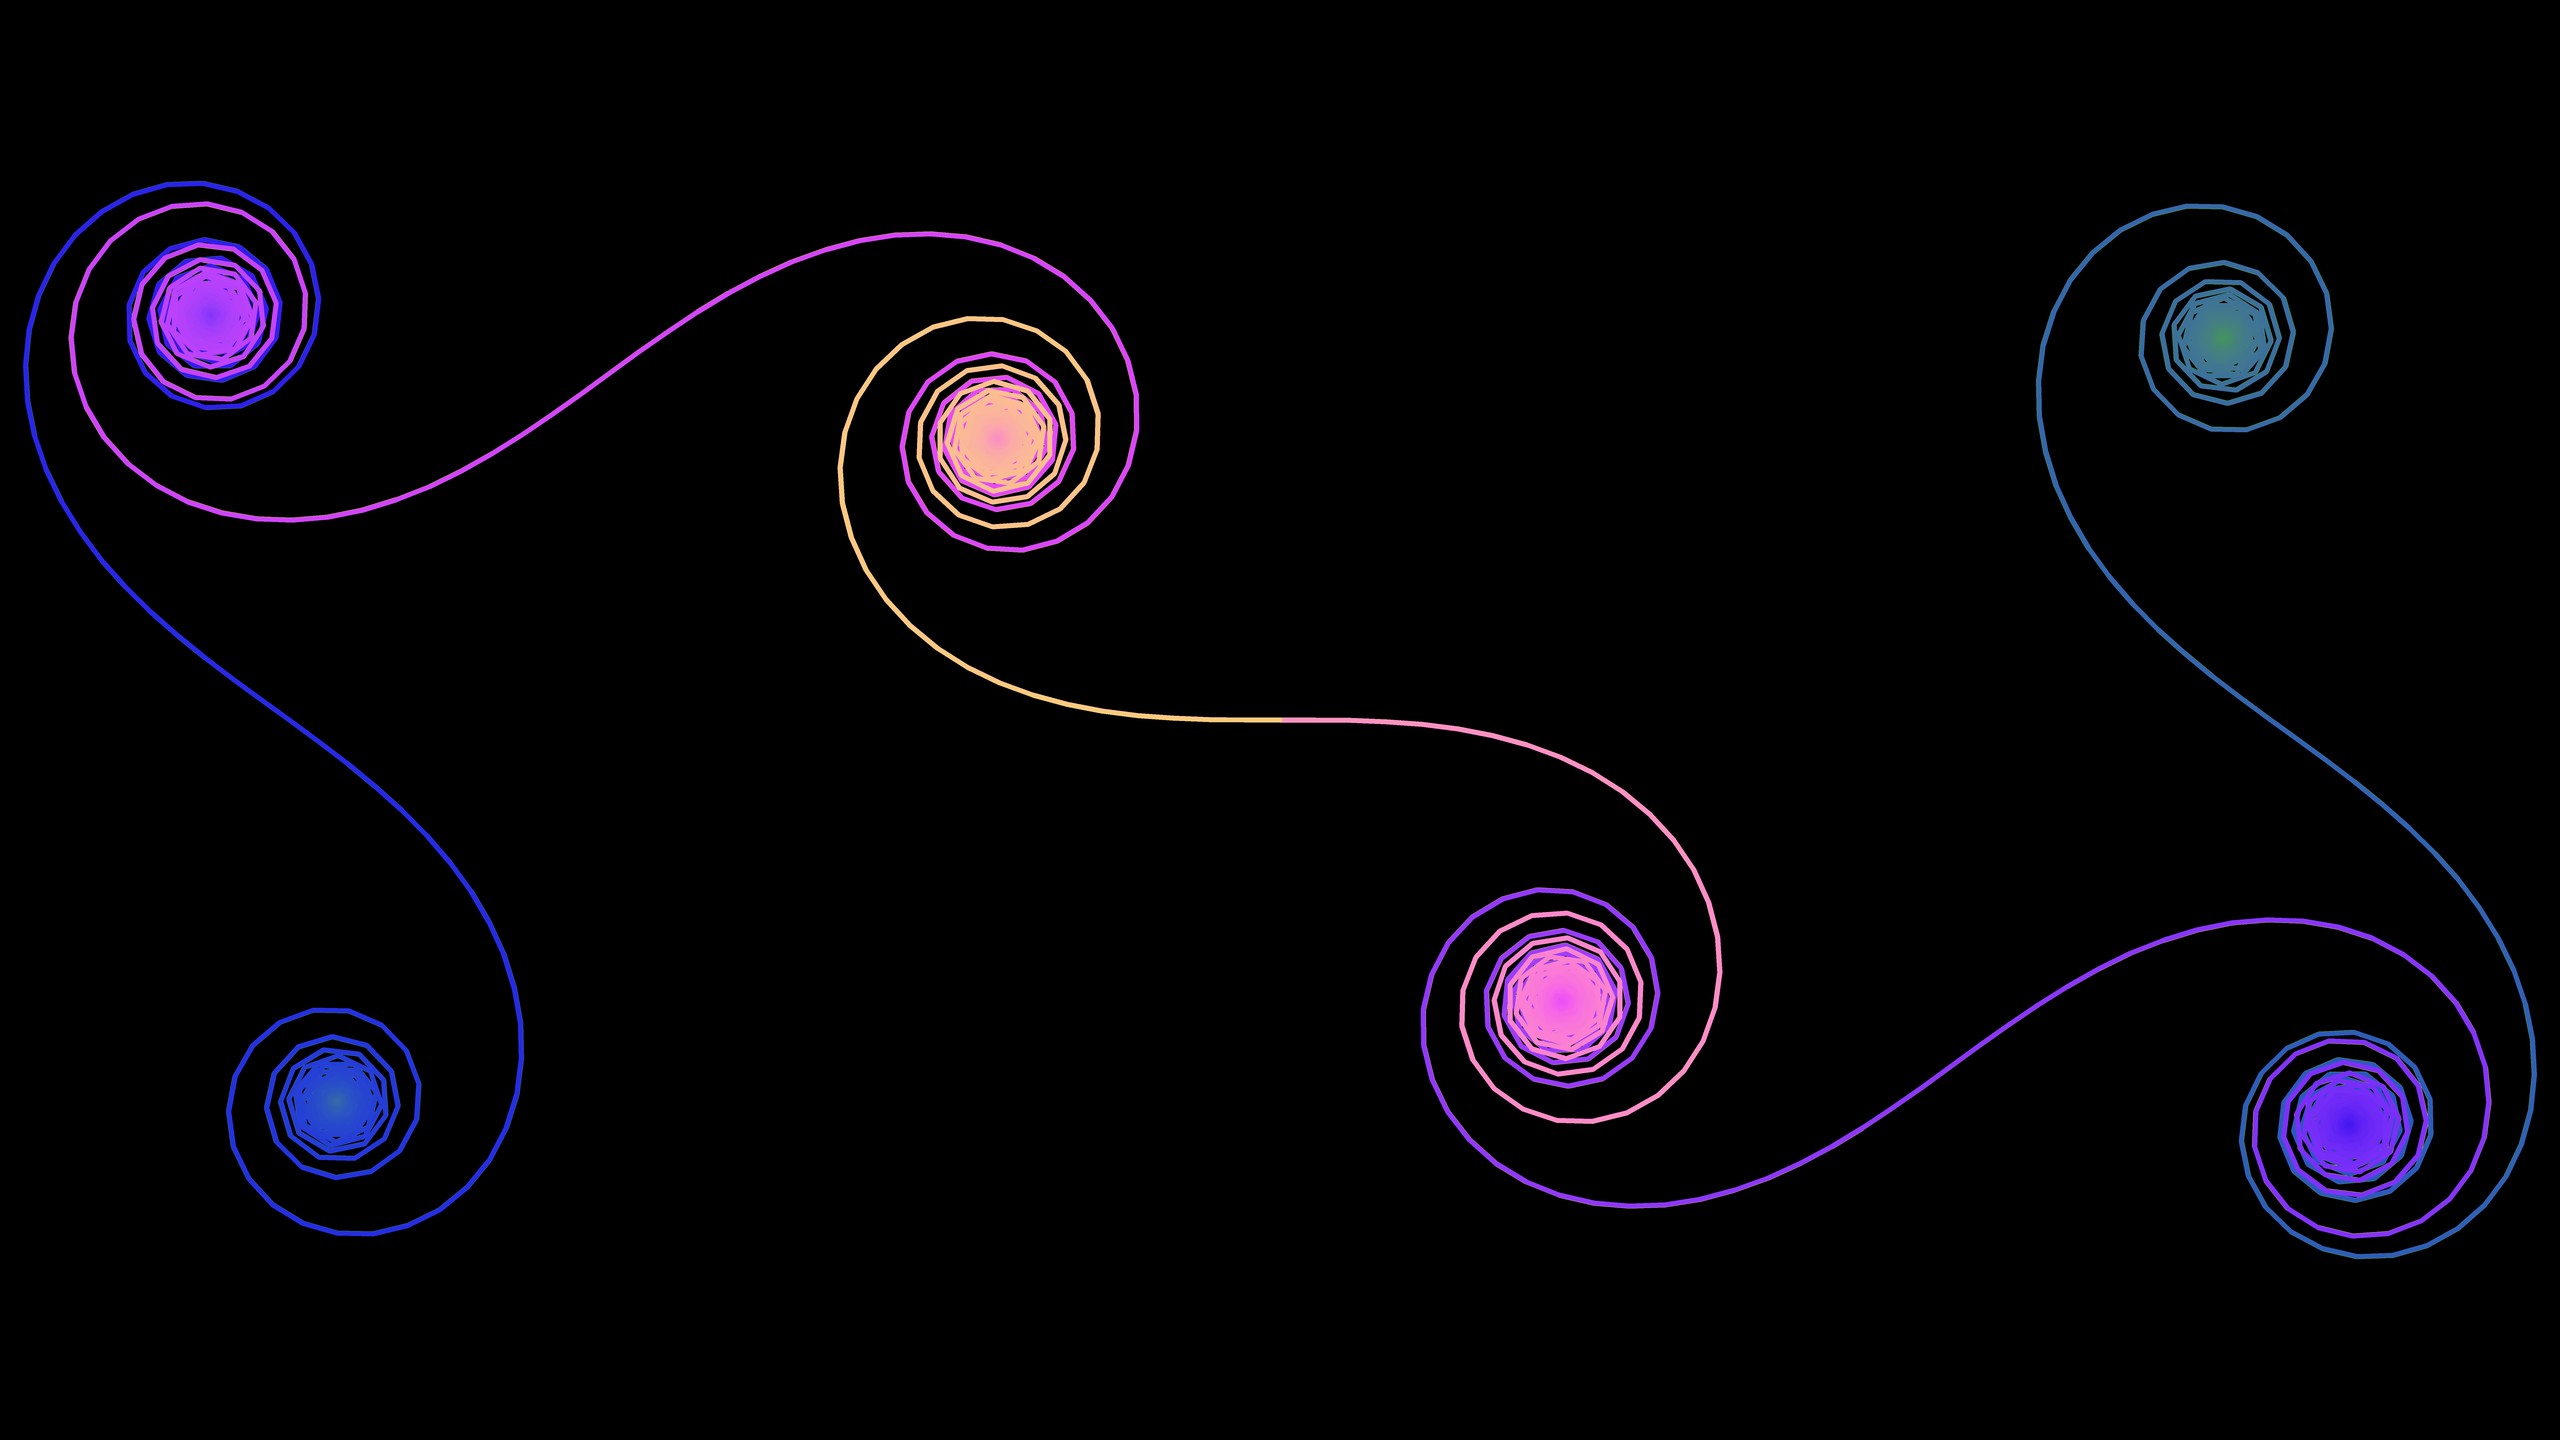
\includegraphics[width=0.3\textwidth]{./horizontal/tfa_046_p=005_q=2506_theta=0-71828_0_00_b_cyclic_mygbm_30_95_c78_Euler-Euler-Spiral_black.png}
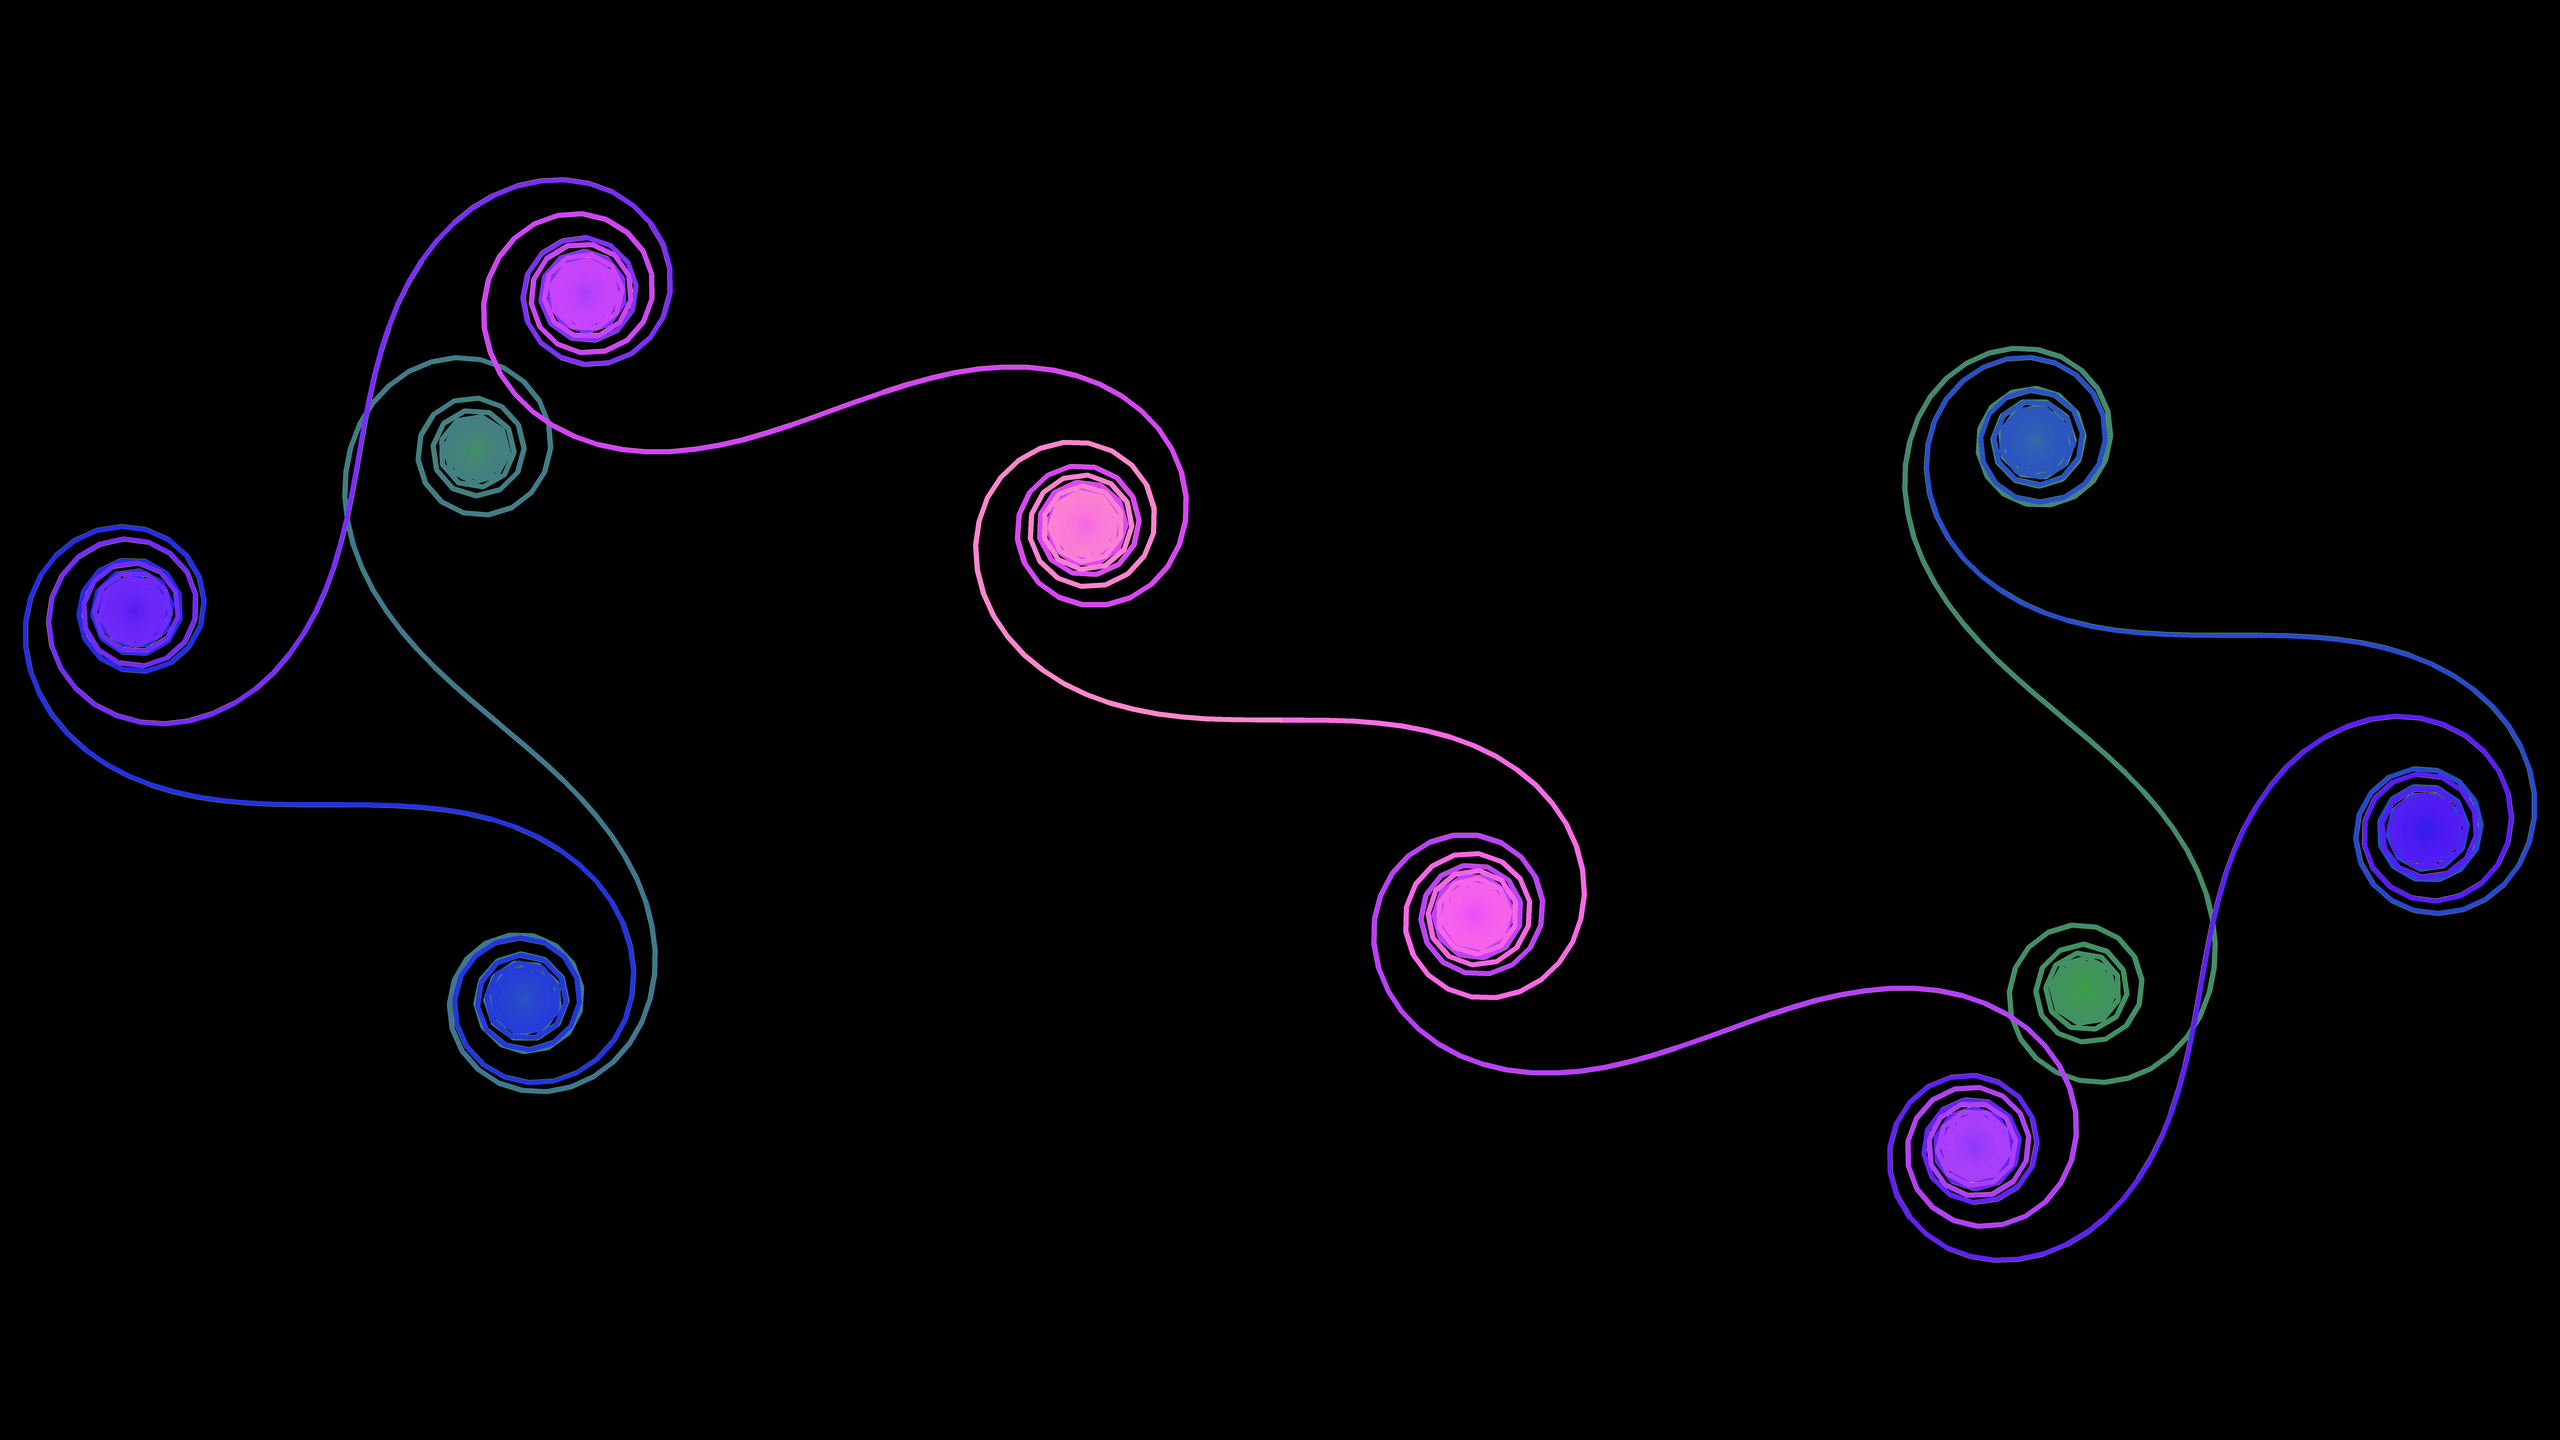
\includegraphics[width=0.3\textwidth]{./horizontal/tfa_046_p=009_q=4510_theta=0-71840_0_00_b_cyclic_mygbm_30_95_c78_Euler-Euler-Spiral_black.png}
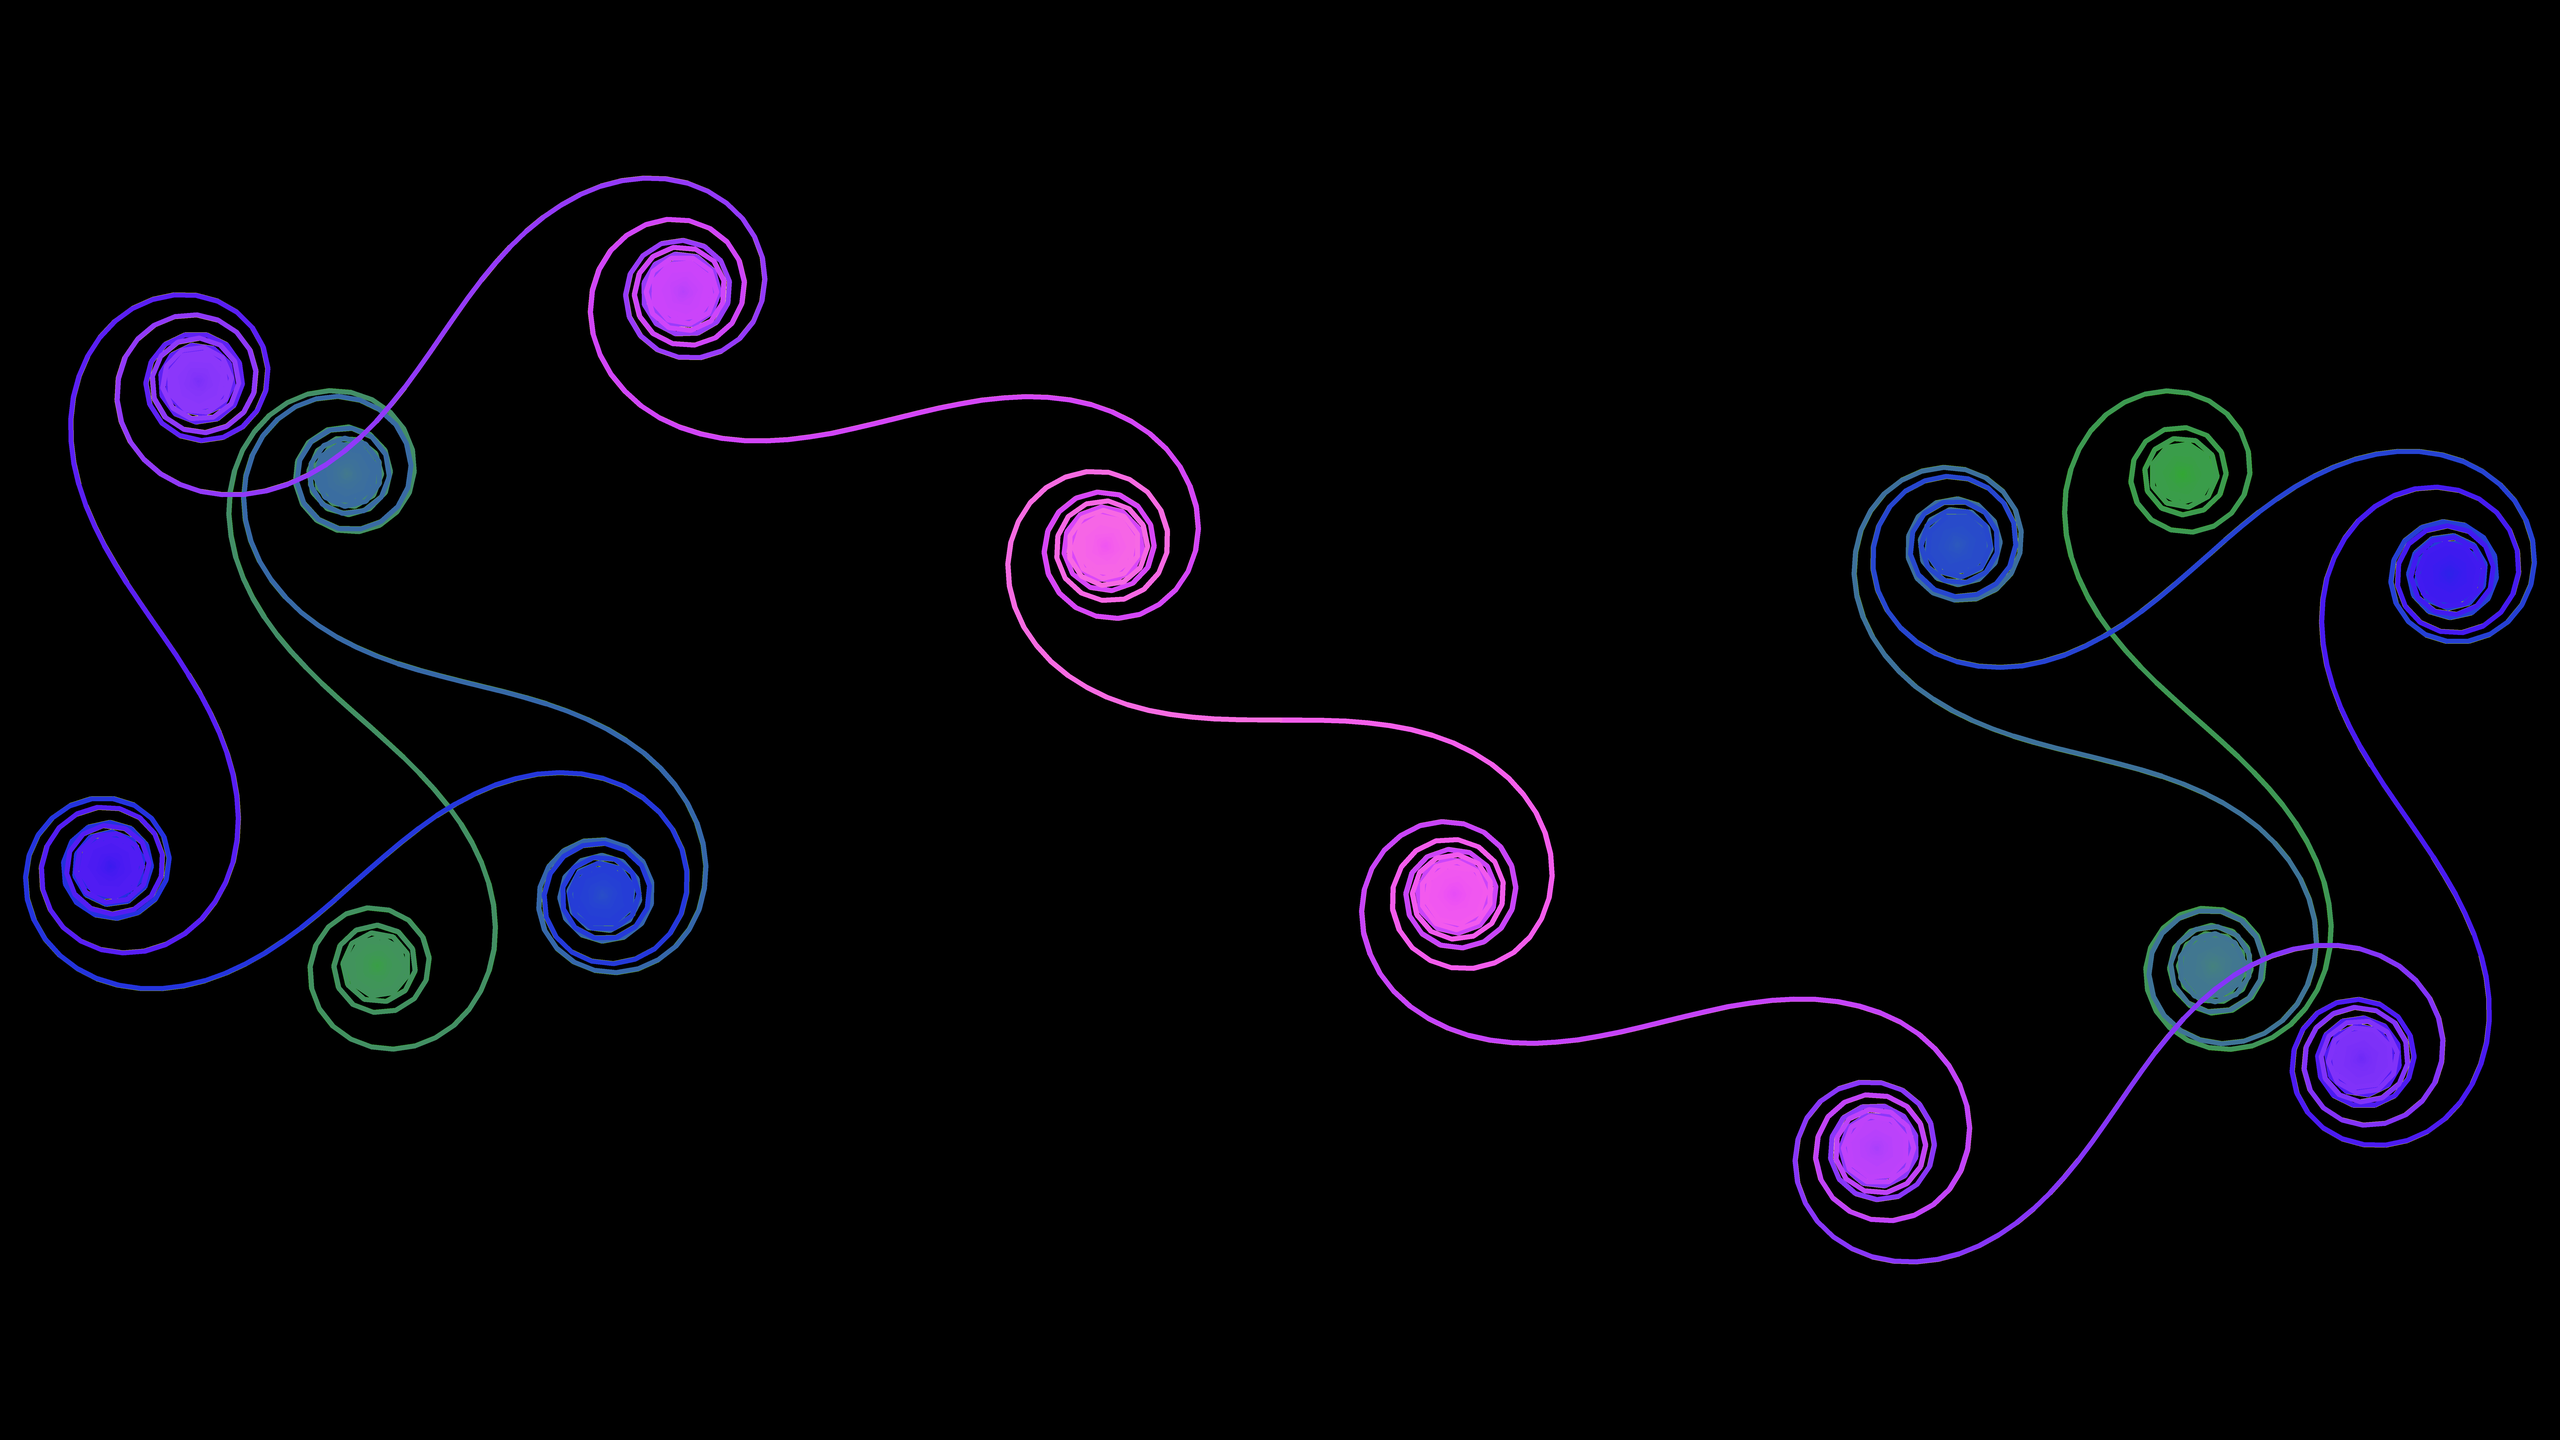
\includegraphics[width=0.3\textwidth]{./horizontal/tfa_046_p=013_q=6514_theta=0-71845_0_00_b_cyclic_mygbm_30_95_c78_Euler-Euler-Spiral_black.png}

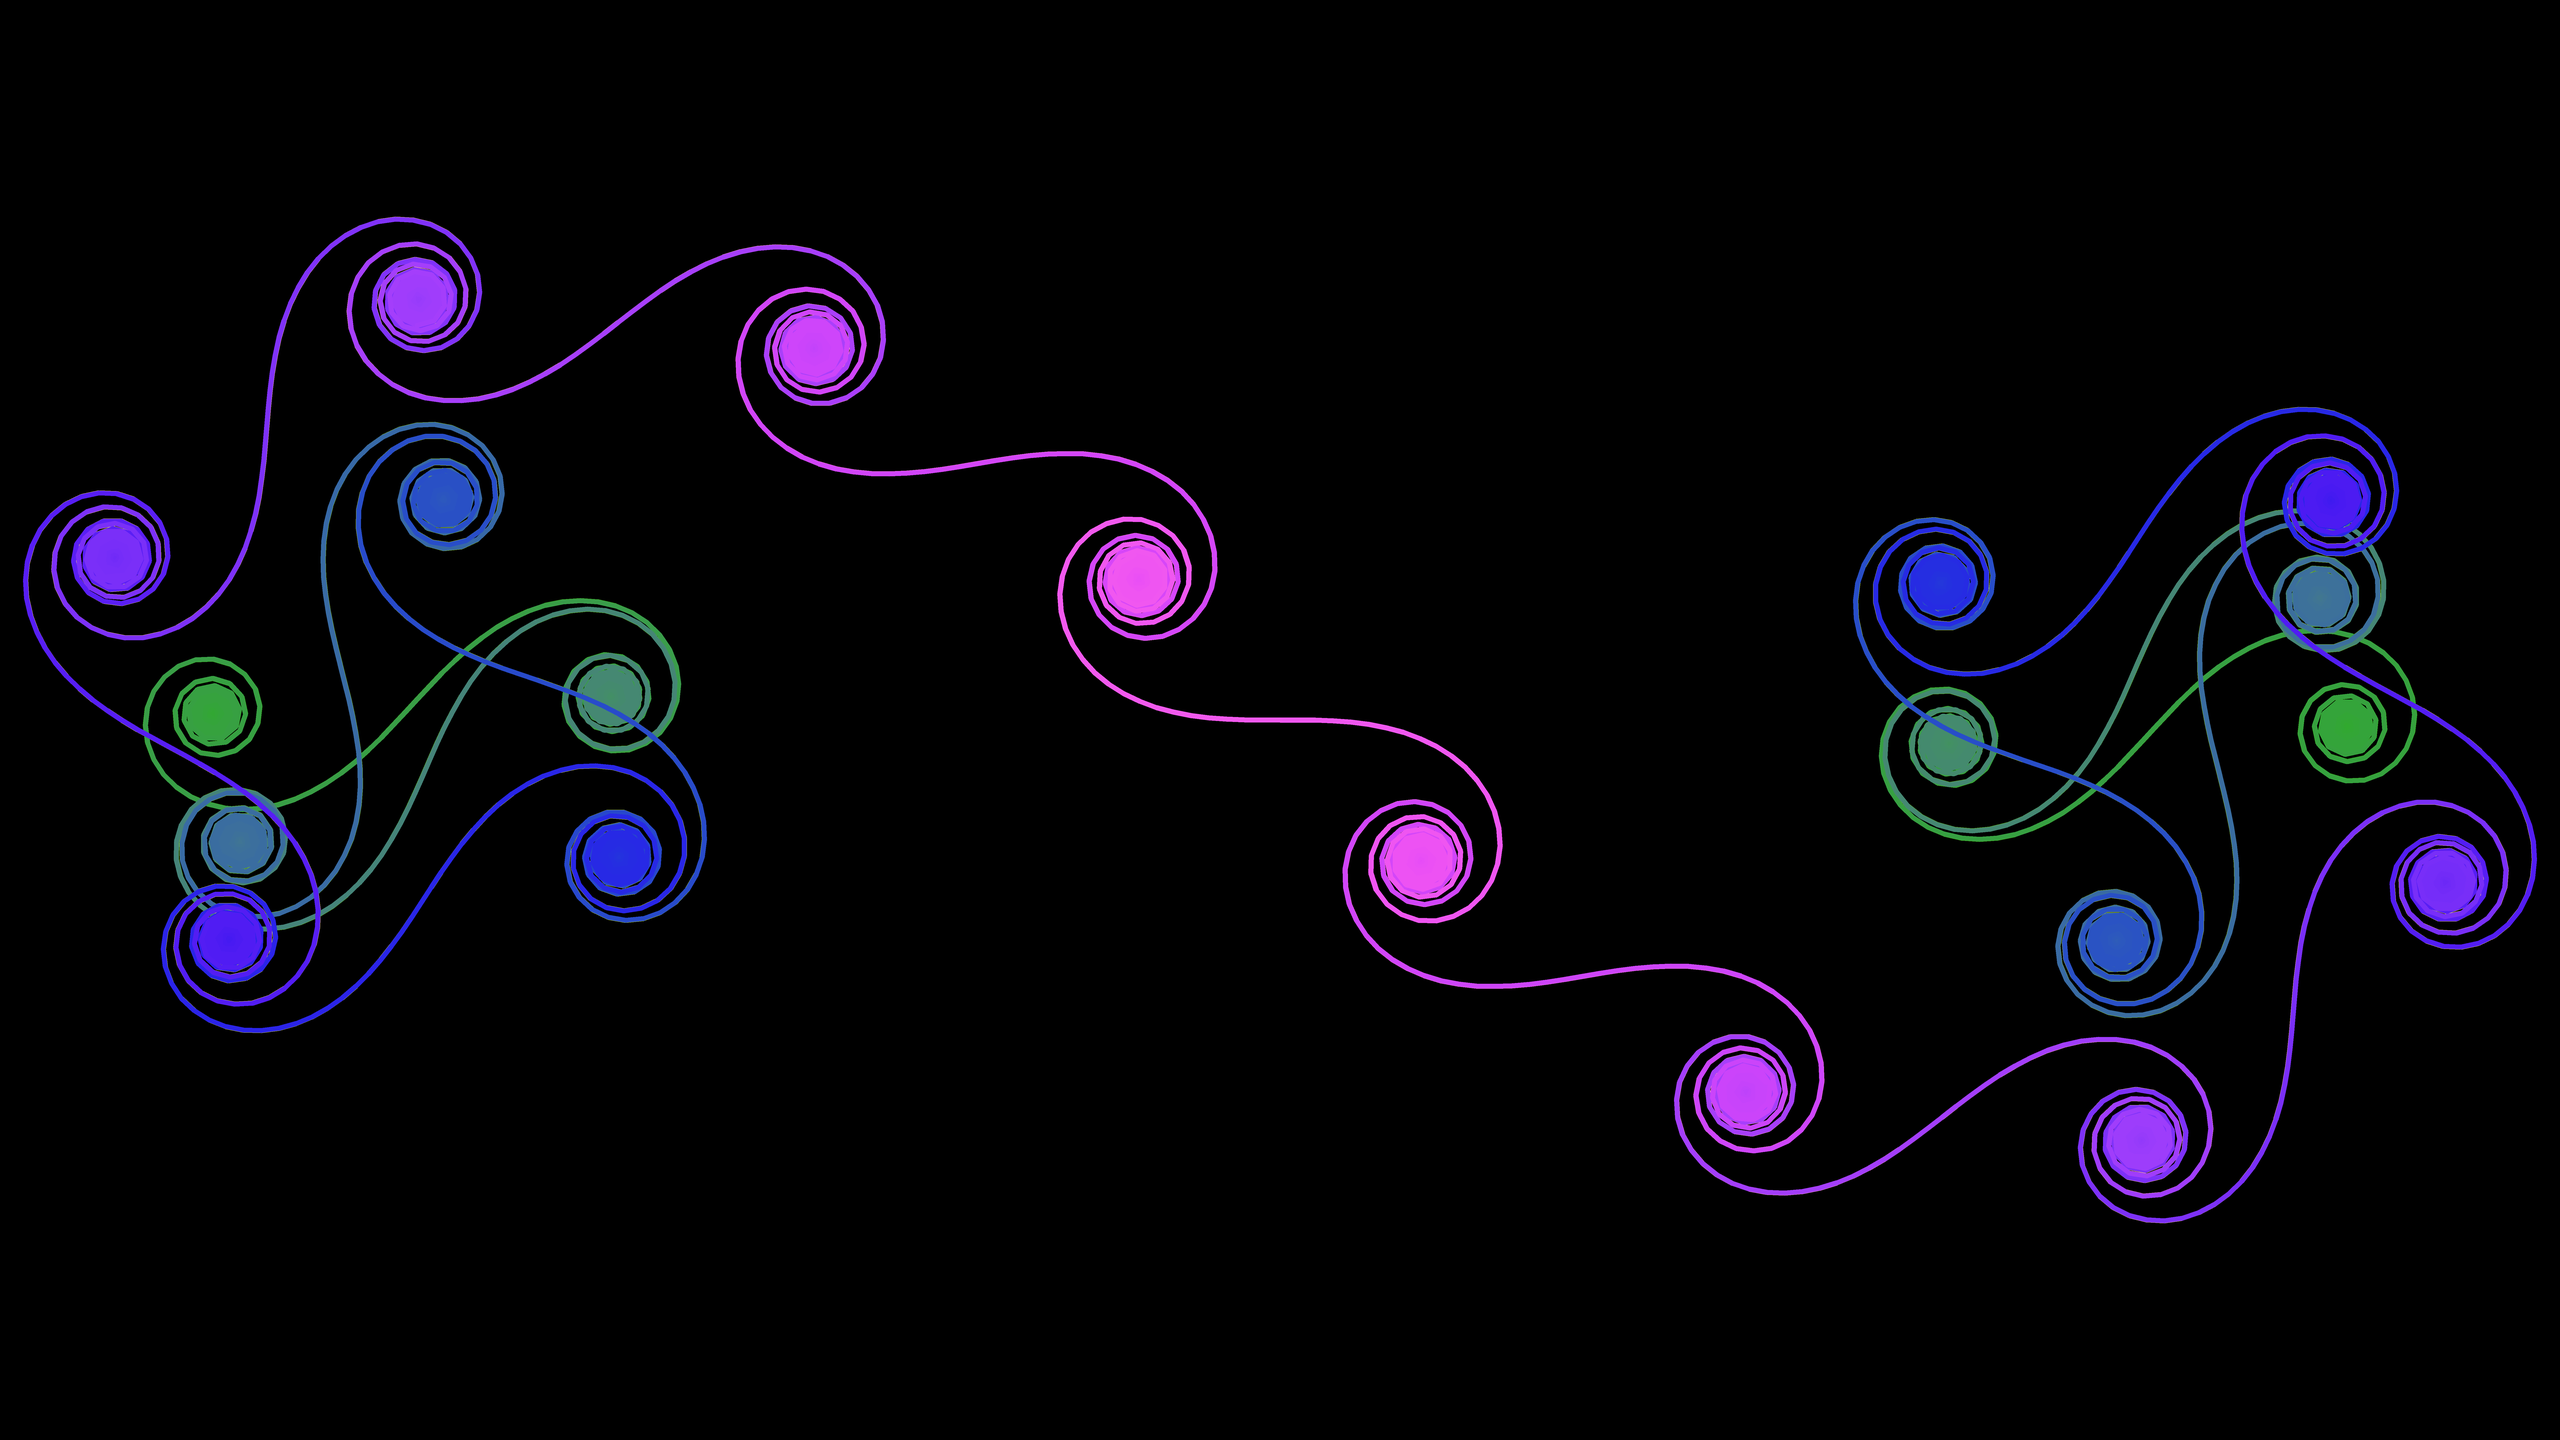
\includegraphics[width=0.3\textwidth]{./horizontal/tfa_046_p=019_q=9520_theta=0-71849_0_00_b_cyclic_mygbm_30_95_c78_Euler-Euler-Spiral_black.png}
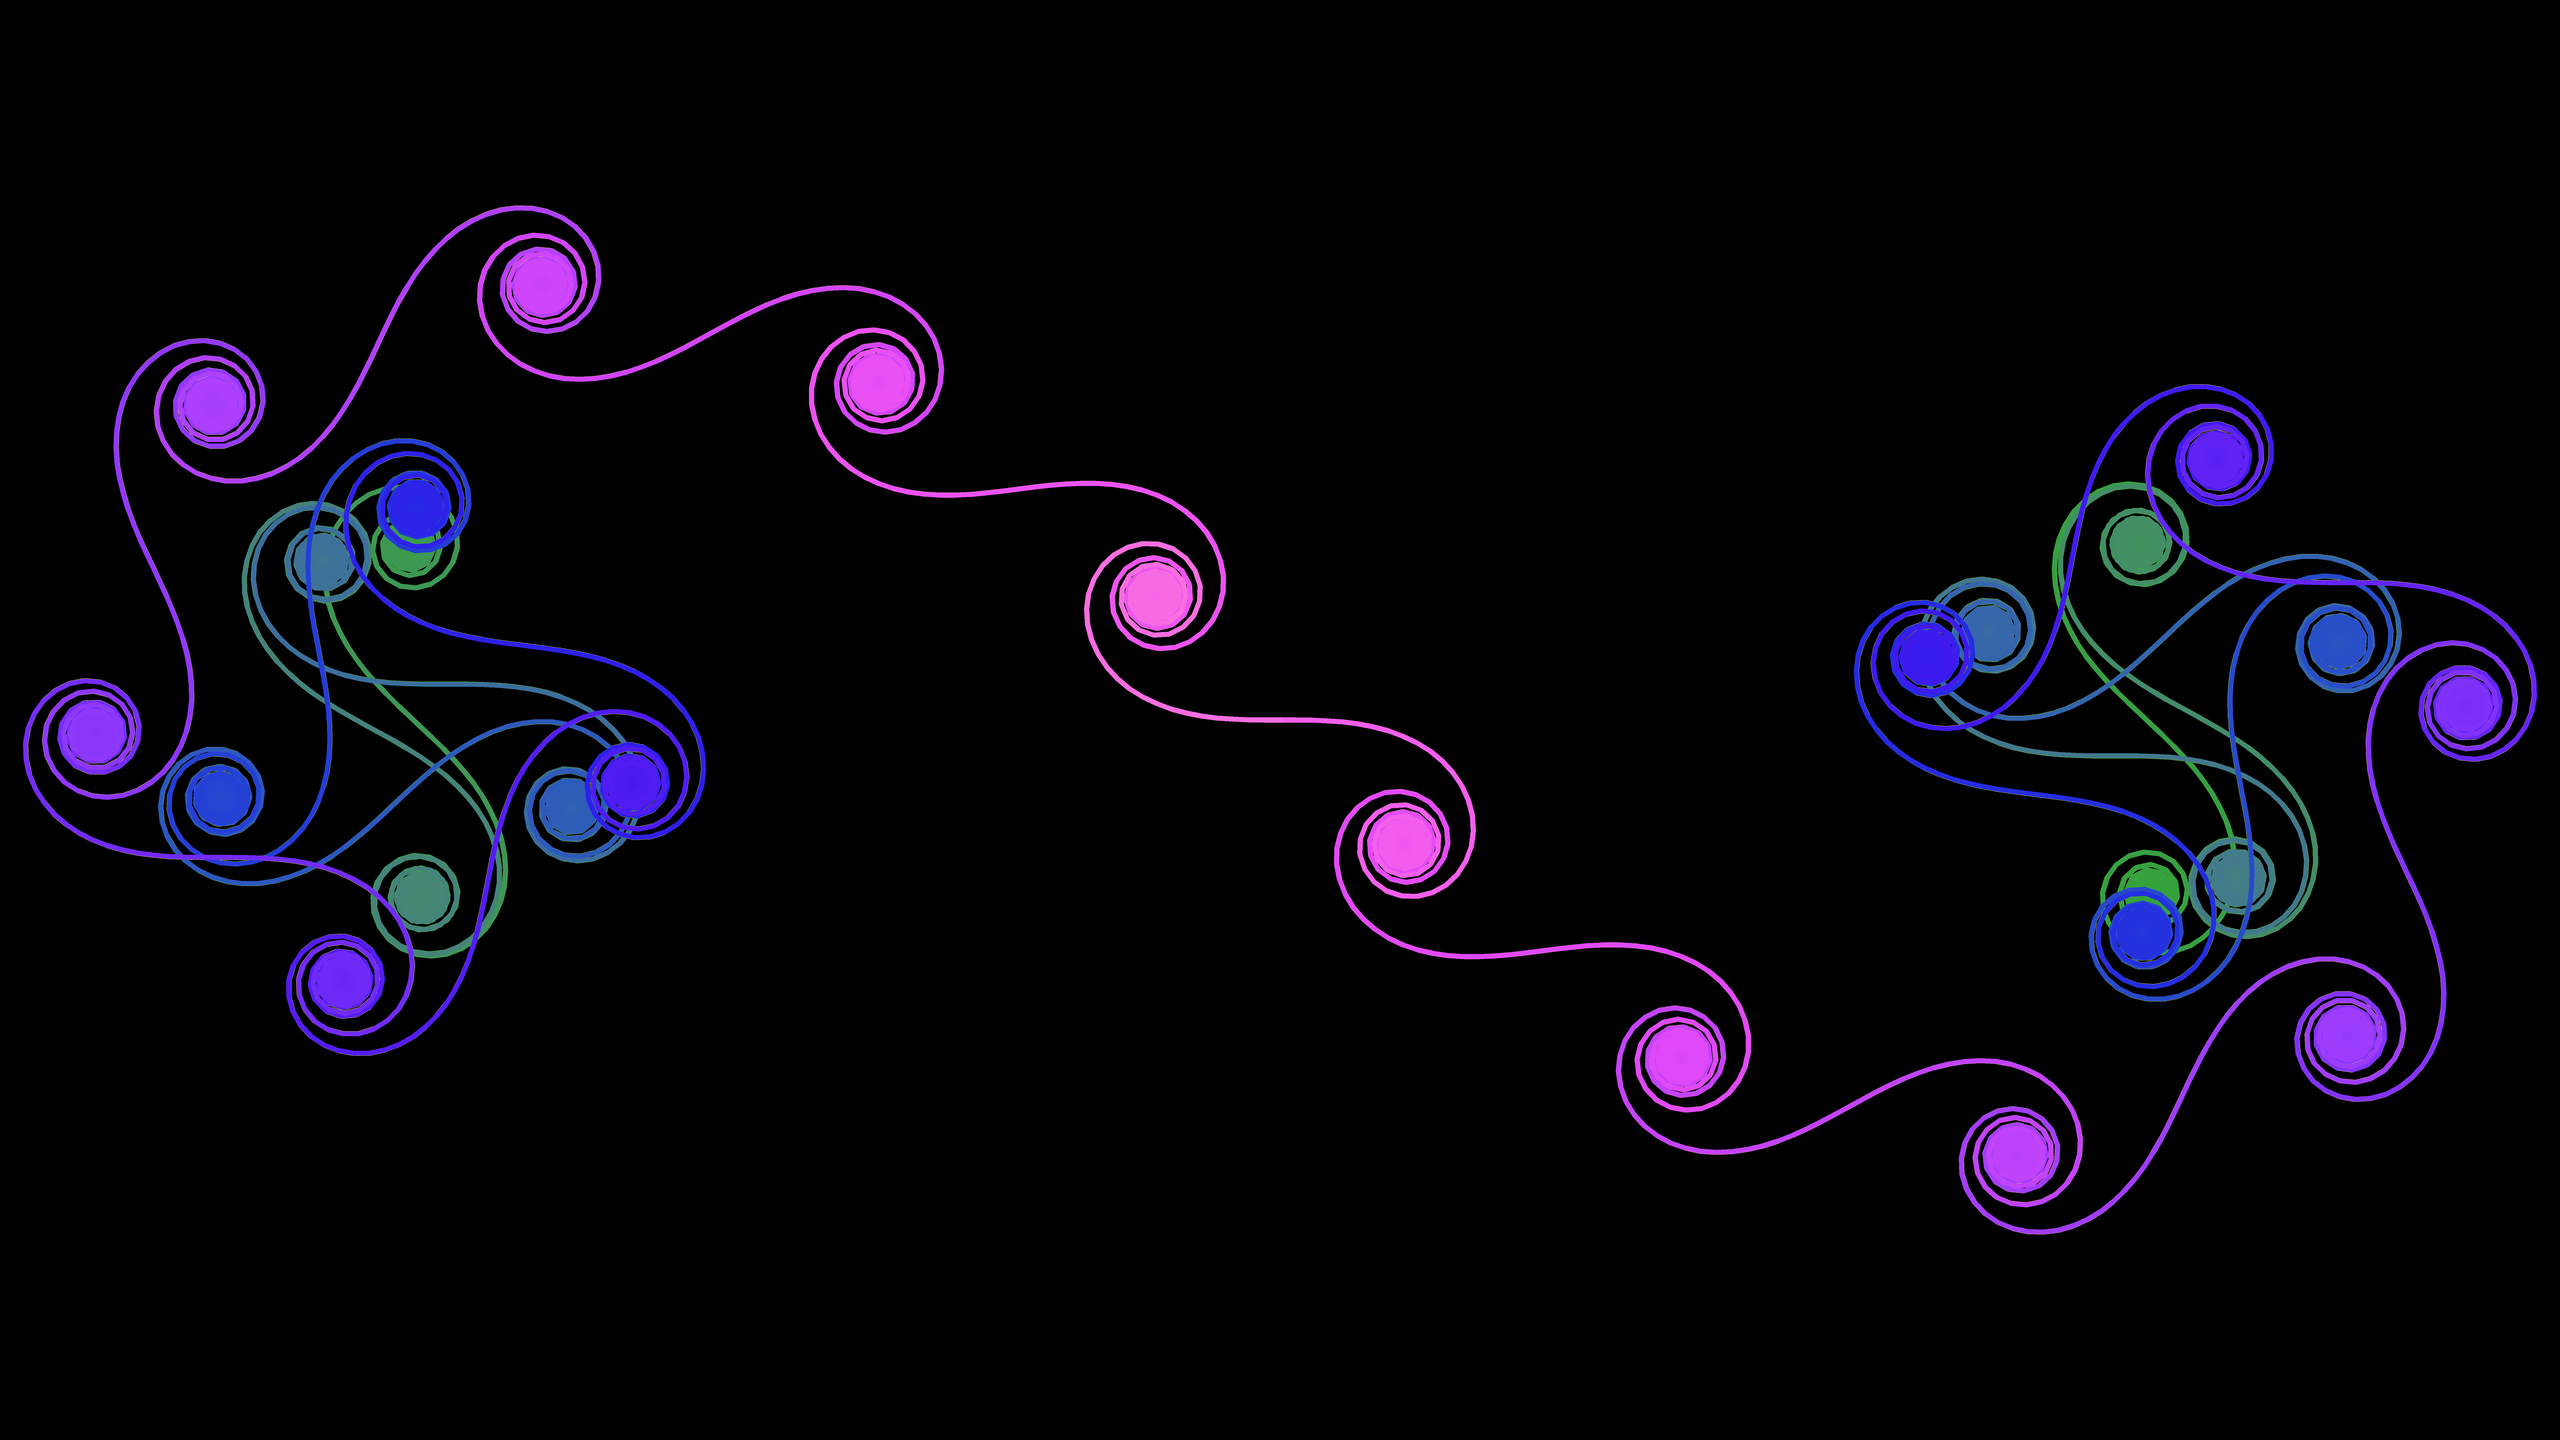
\includegraphics[width=0.3\textwidth]{./horizontal/tfa_046_p=025_q=12526_theta=0-71851_0_00_b_cyclic_mygbm_30_95_c78_Euler-Euler-Spiral_black.png}
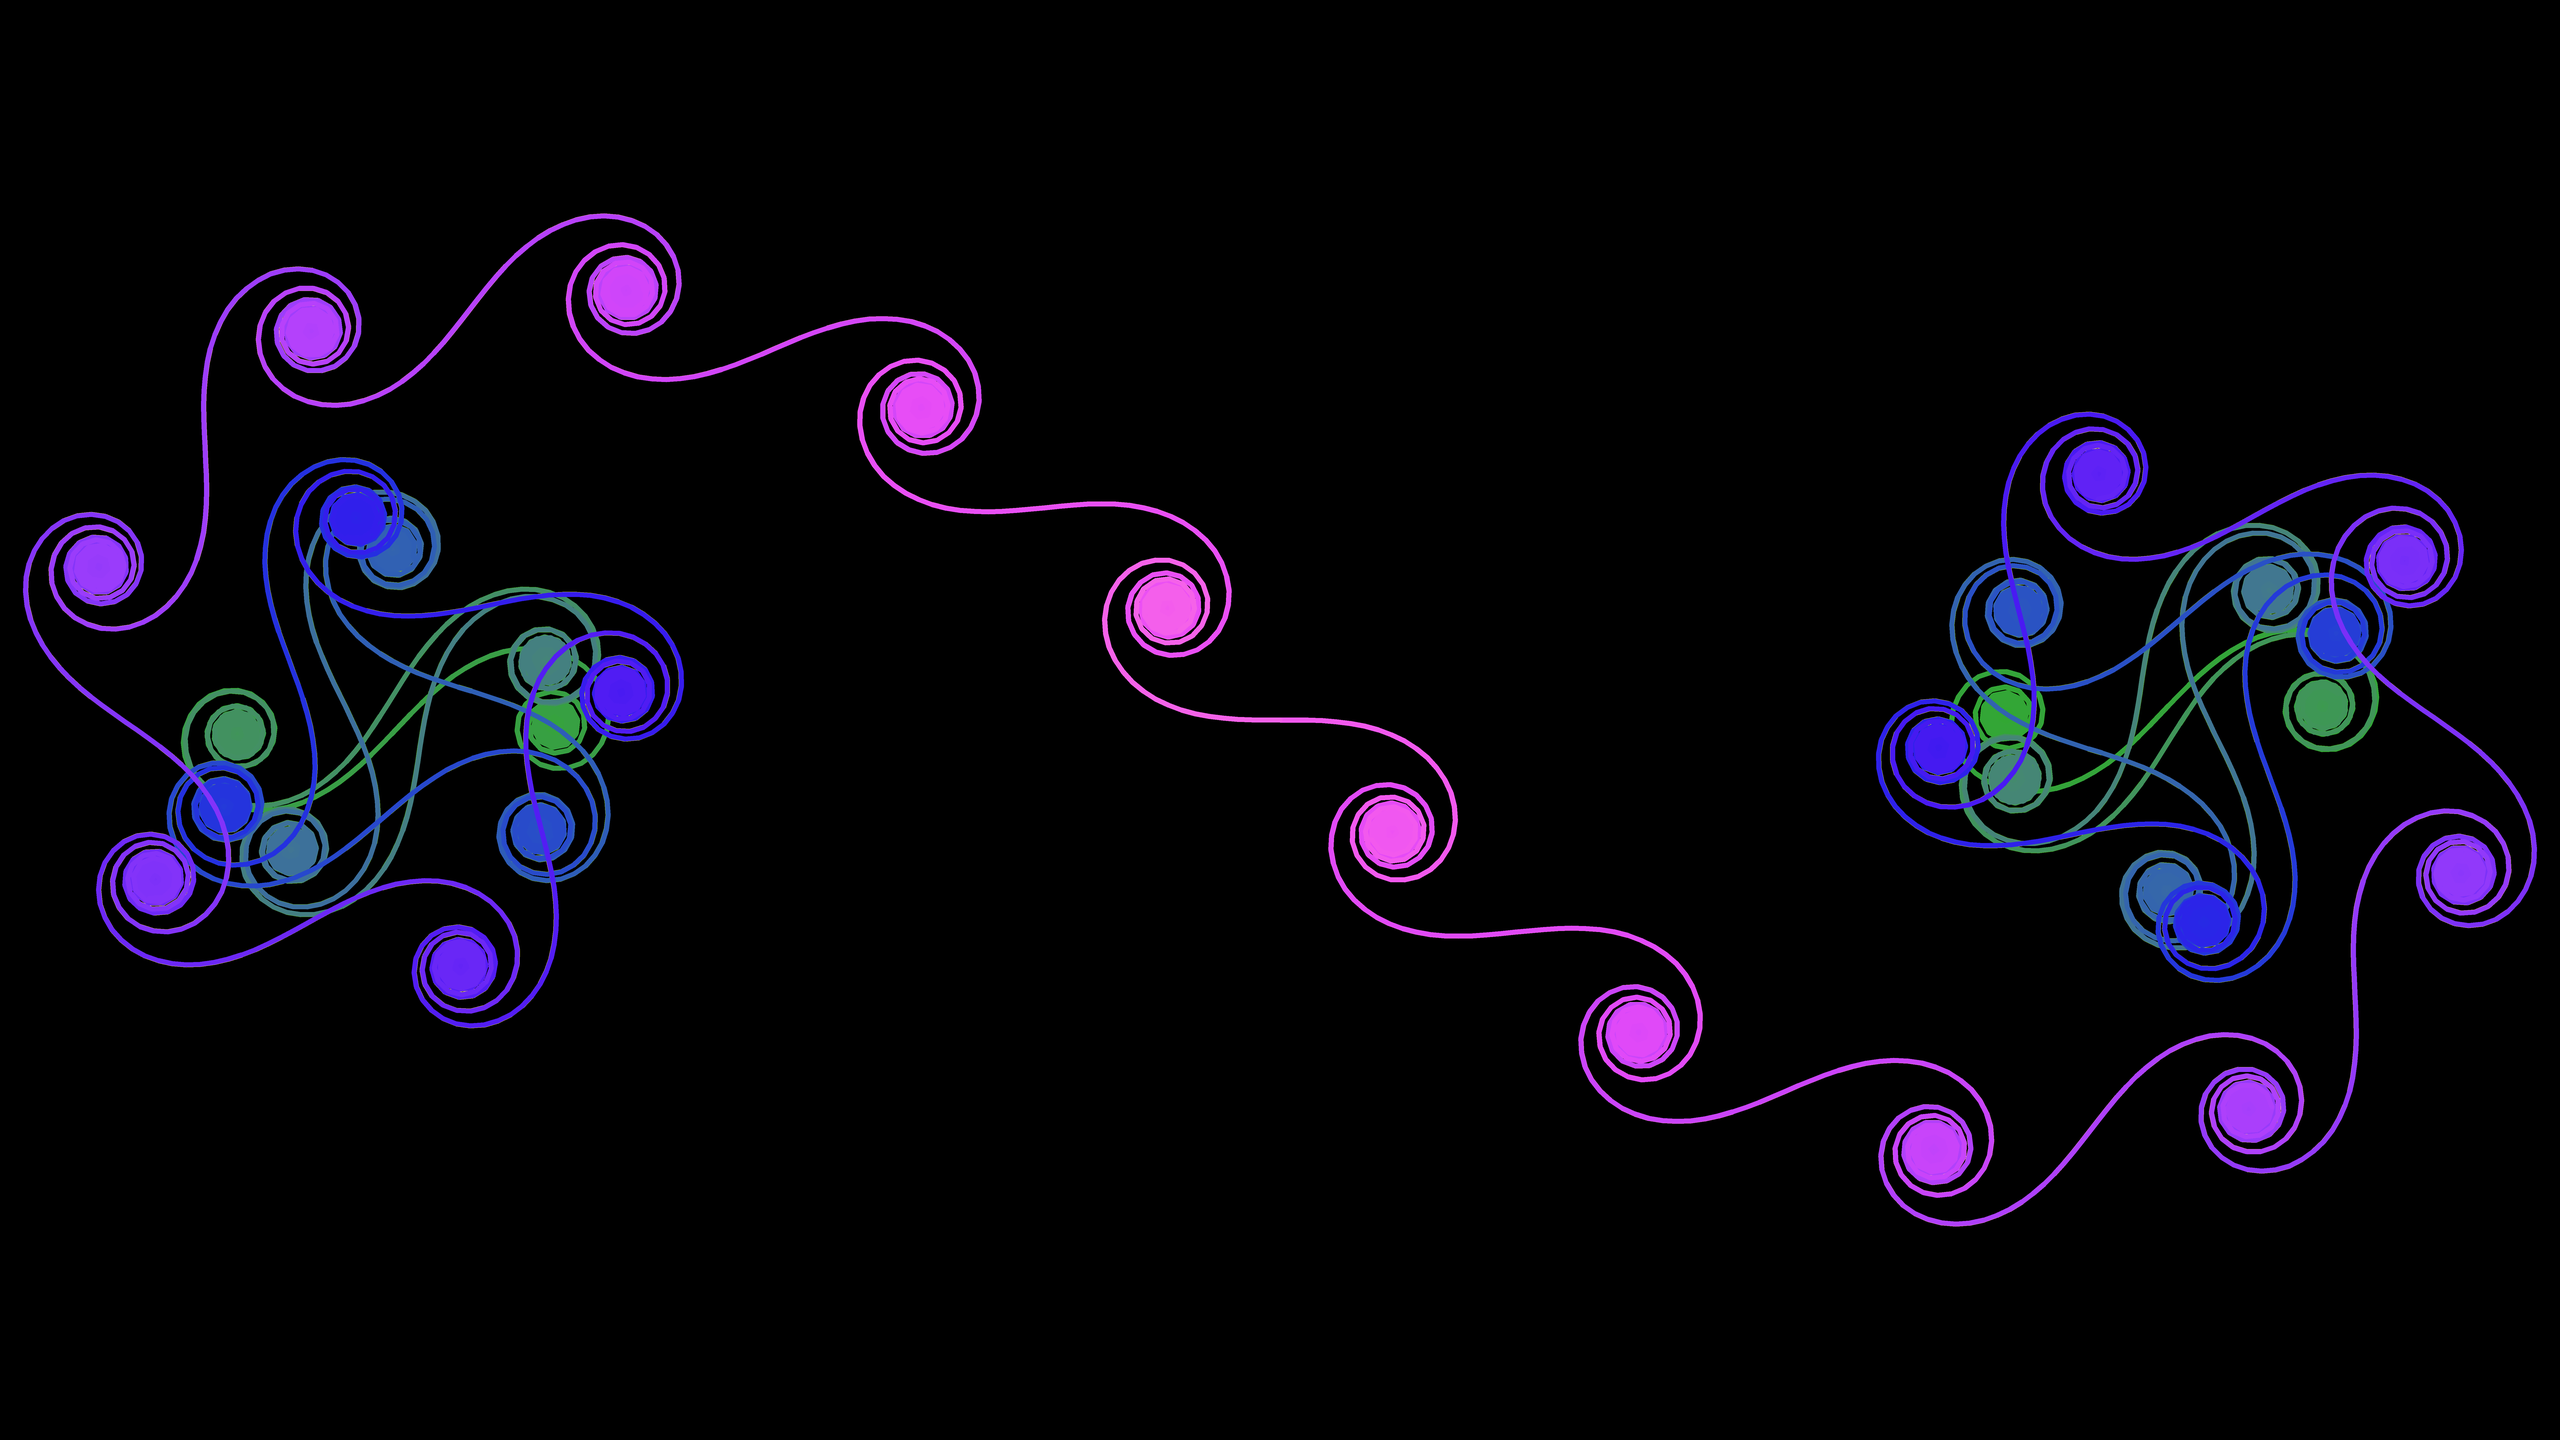
\includegraphics[width=0.3\textwidth]{./horizontal/tfa_046_p=031_q=15532_theta=0-71852_0_00_b_cyclic_mygbm_30_95_c78_Euler-Euler-Spiral_black.png}

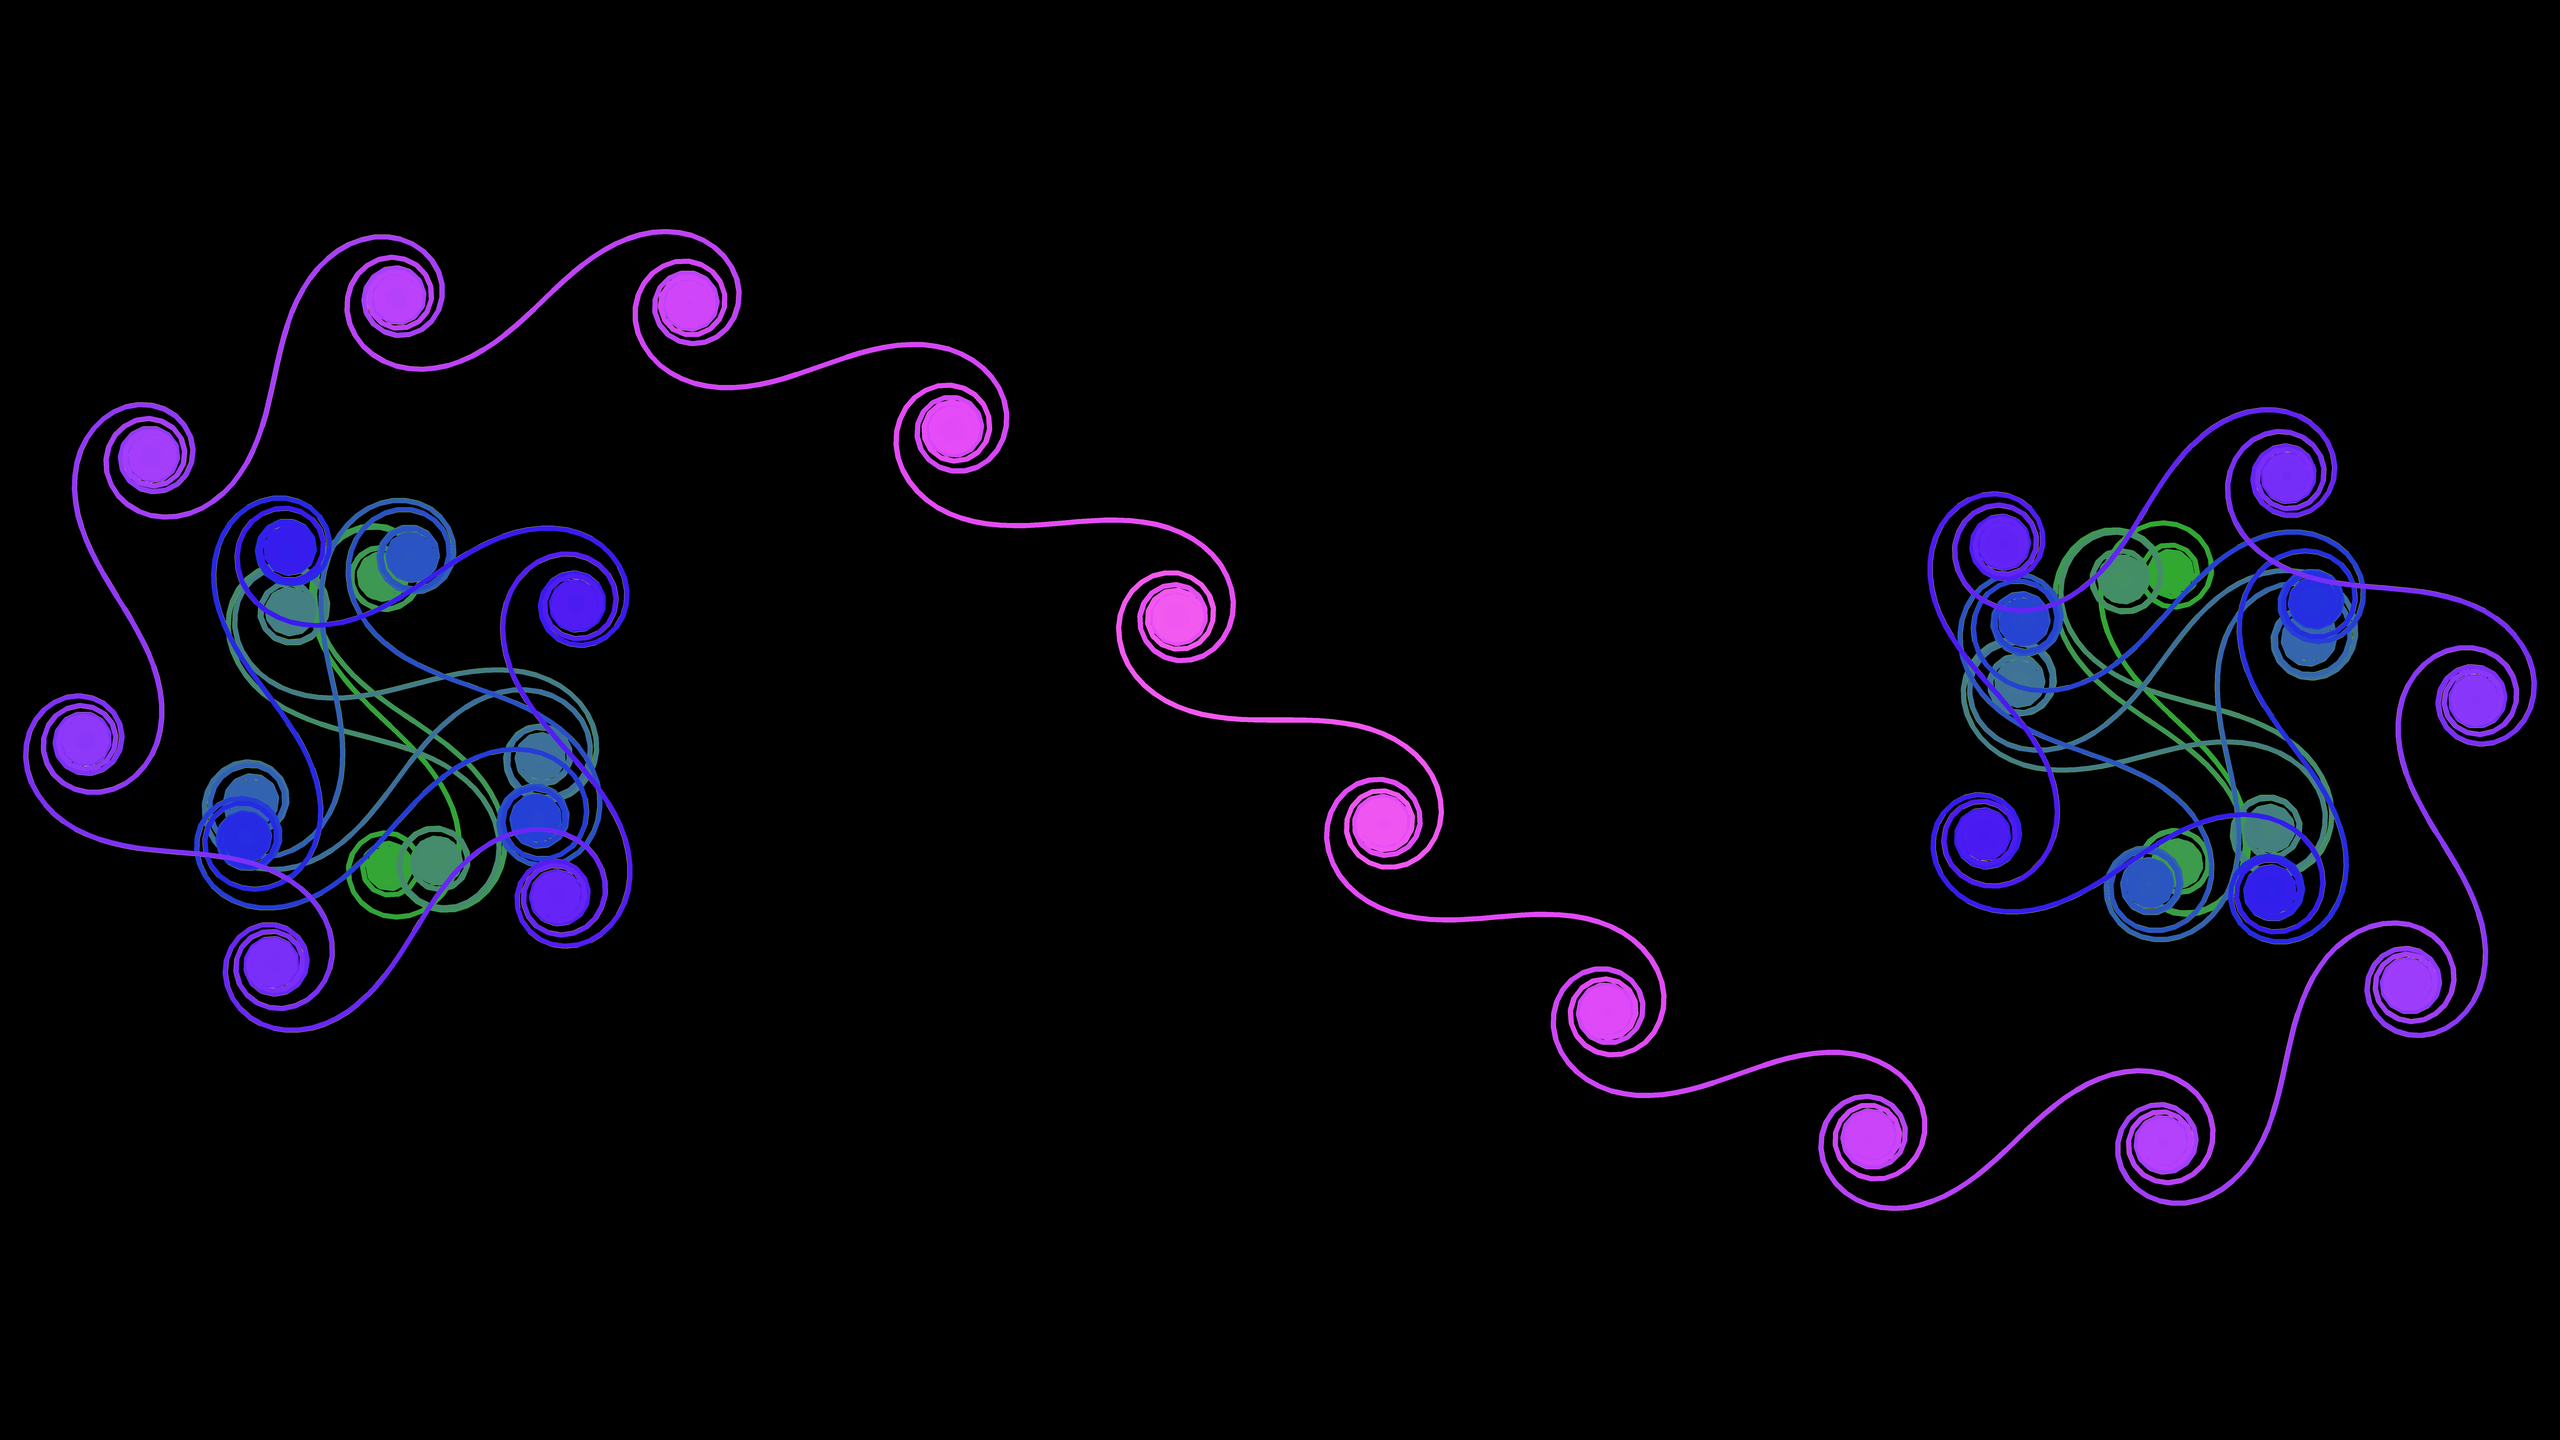
\includegraphics[width=0.3\textwidth]{./horizontal/tfa_046_p=037_q=18538_theta=0-71852_0_00_b_cyclic_mygbm_30_95_c78_Euler-Euler-Spiral_black.png}
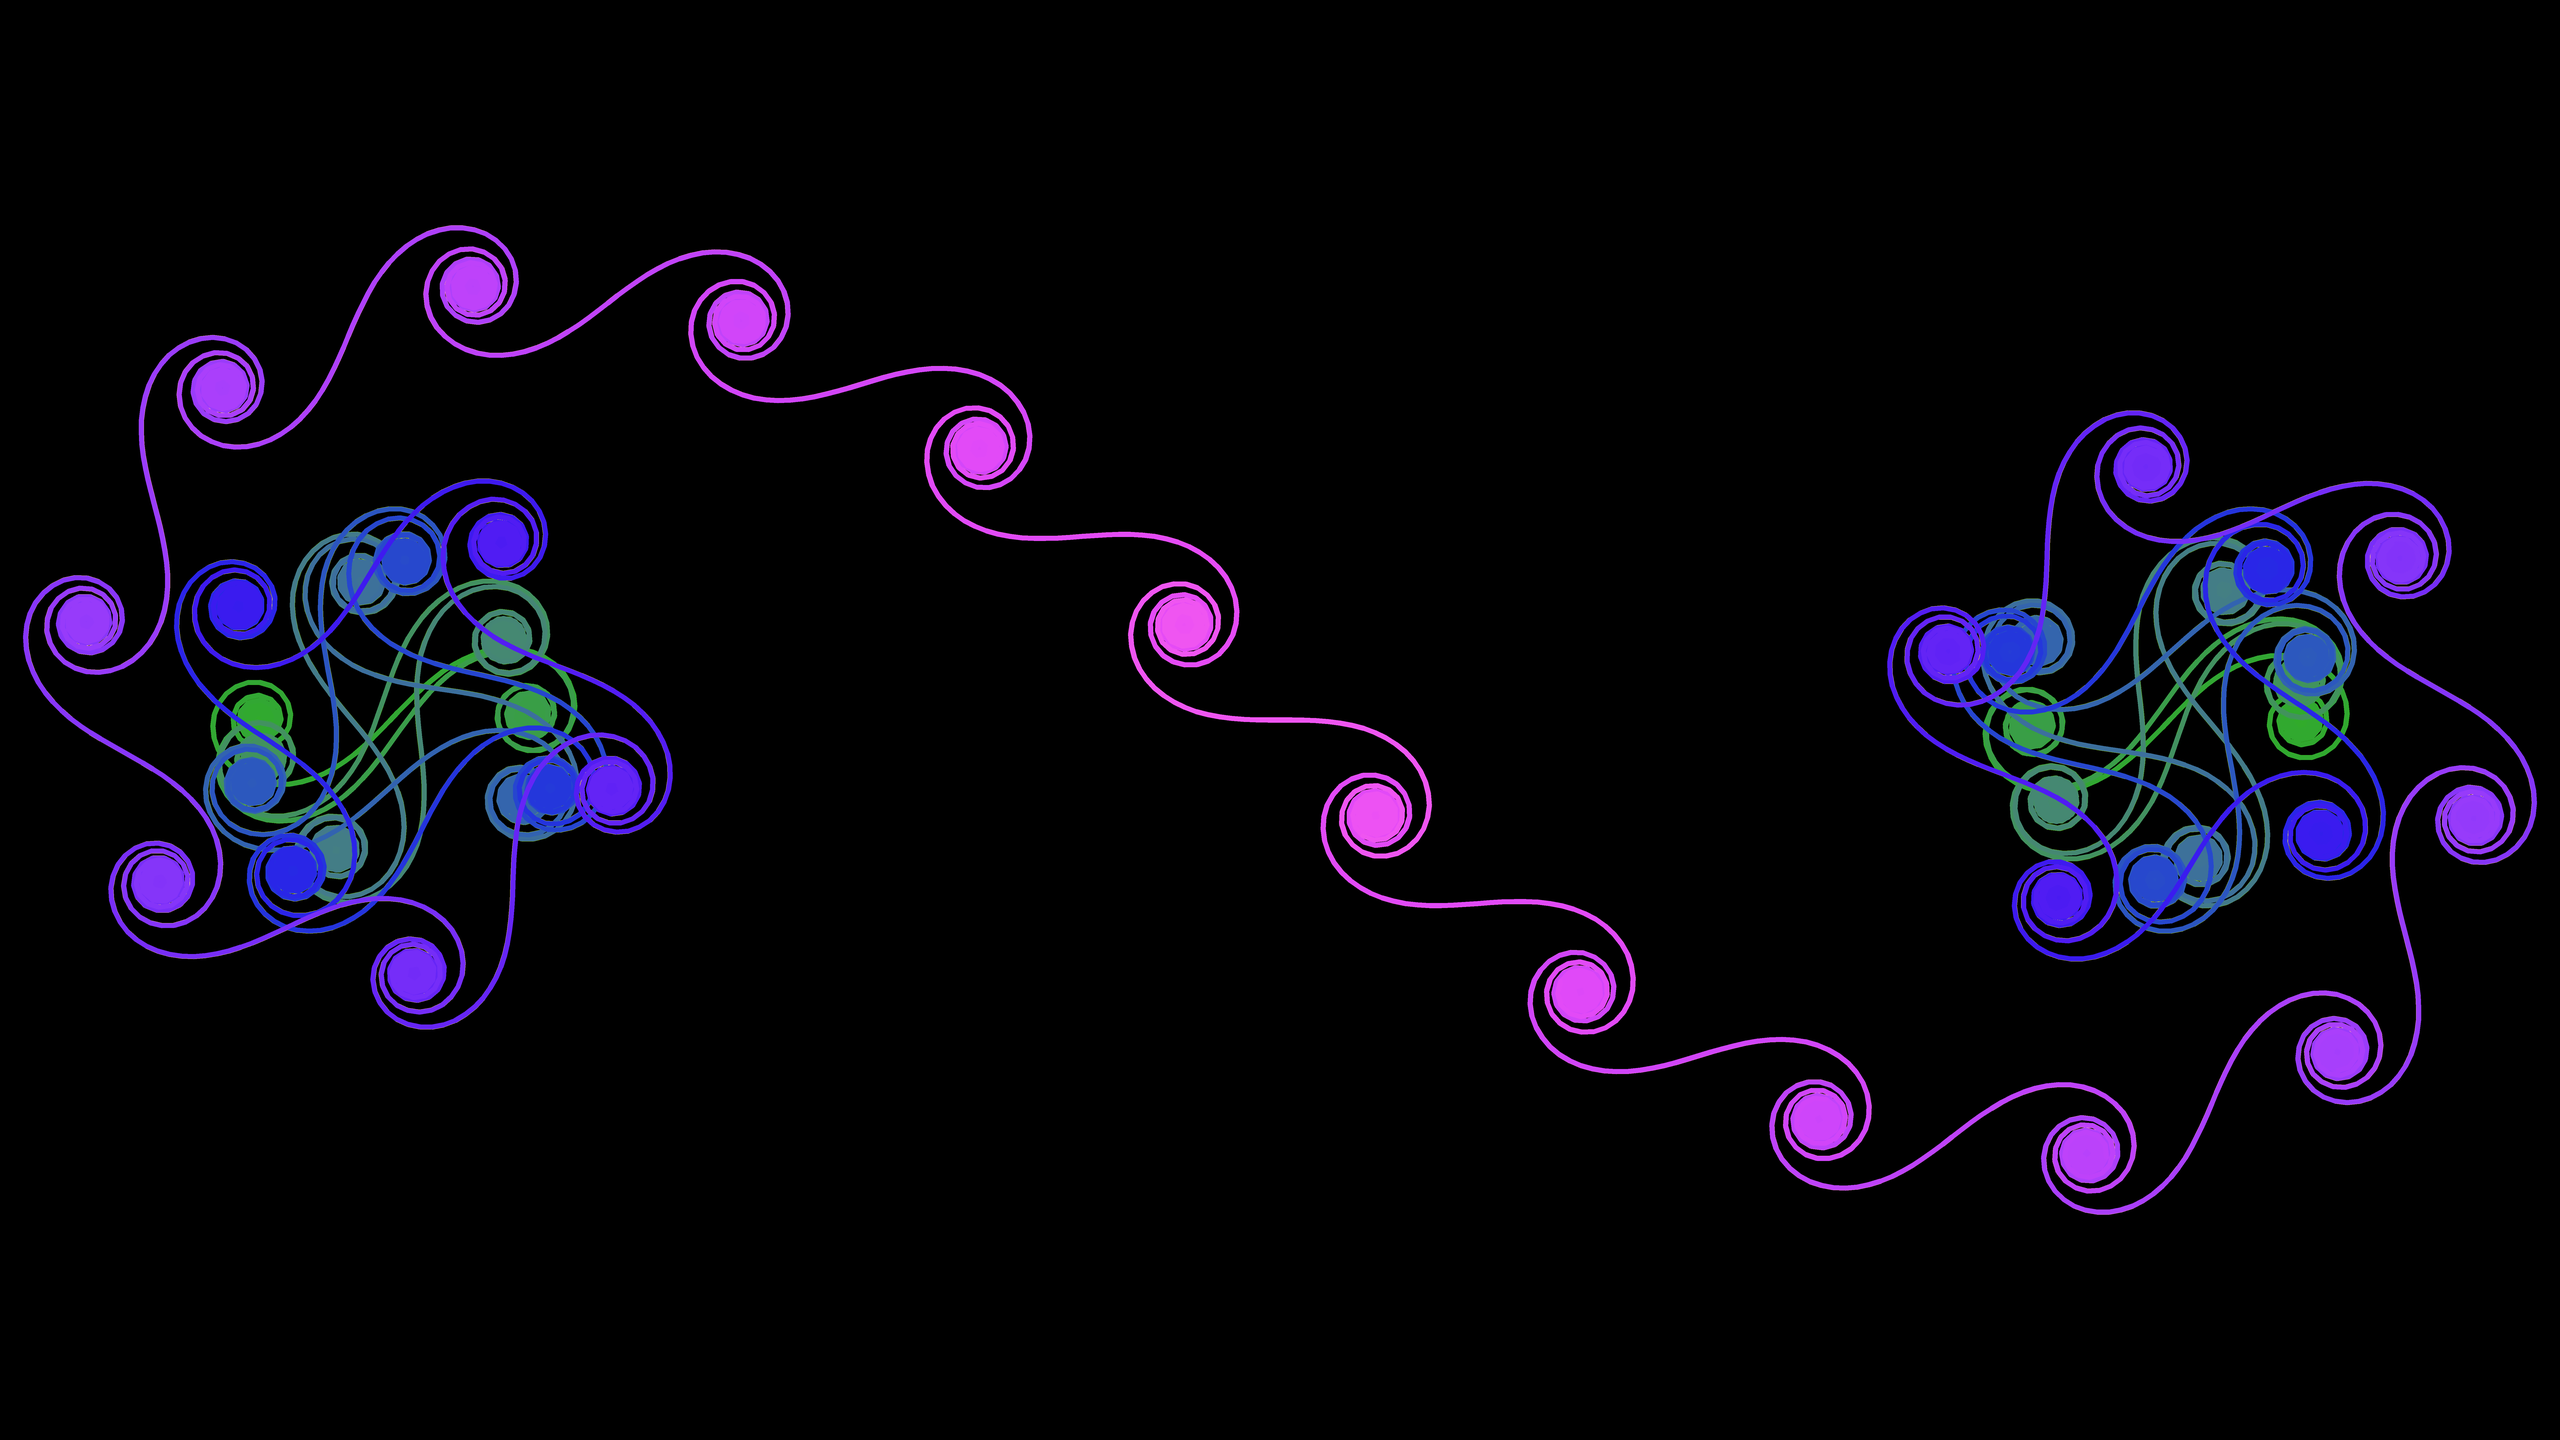
\includegraphics[width=0.3\textwidth]{./horizontal/tfa_046_p=043_q=21544_theta=0-71853_0_00_b_cyclic_mygbm_30_95_c78_Euler-Euler-Spiral_black.png}
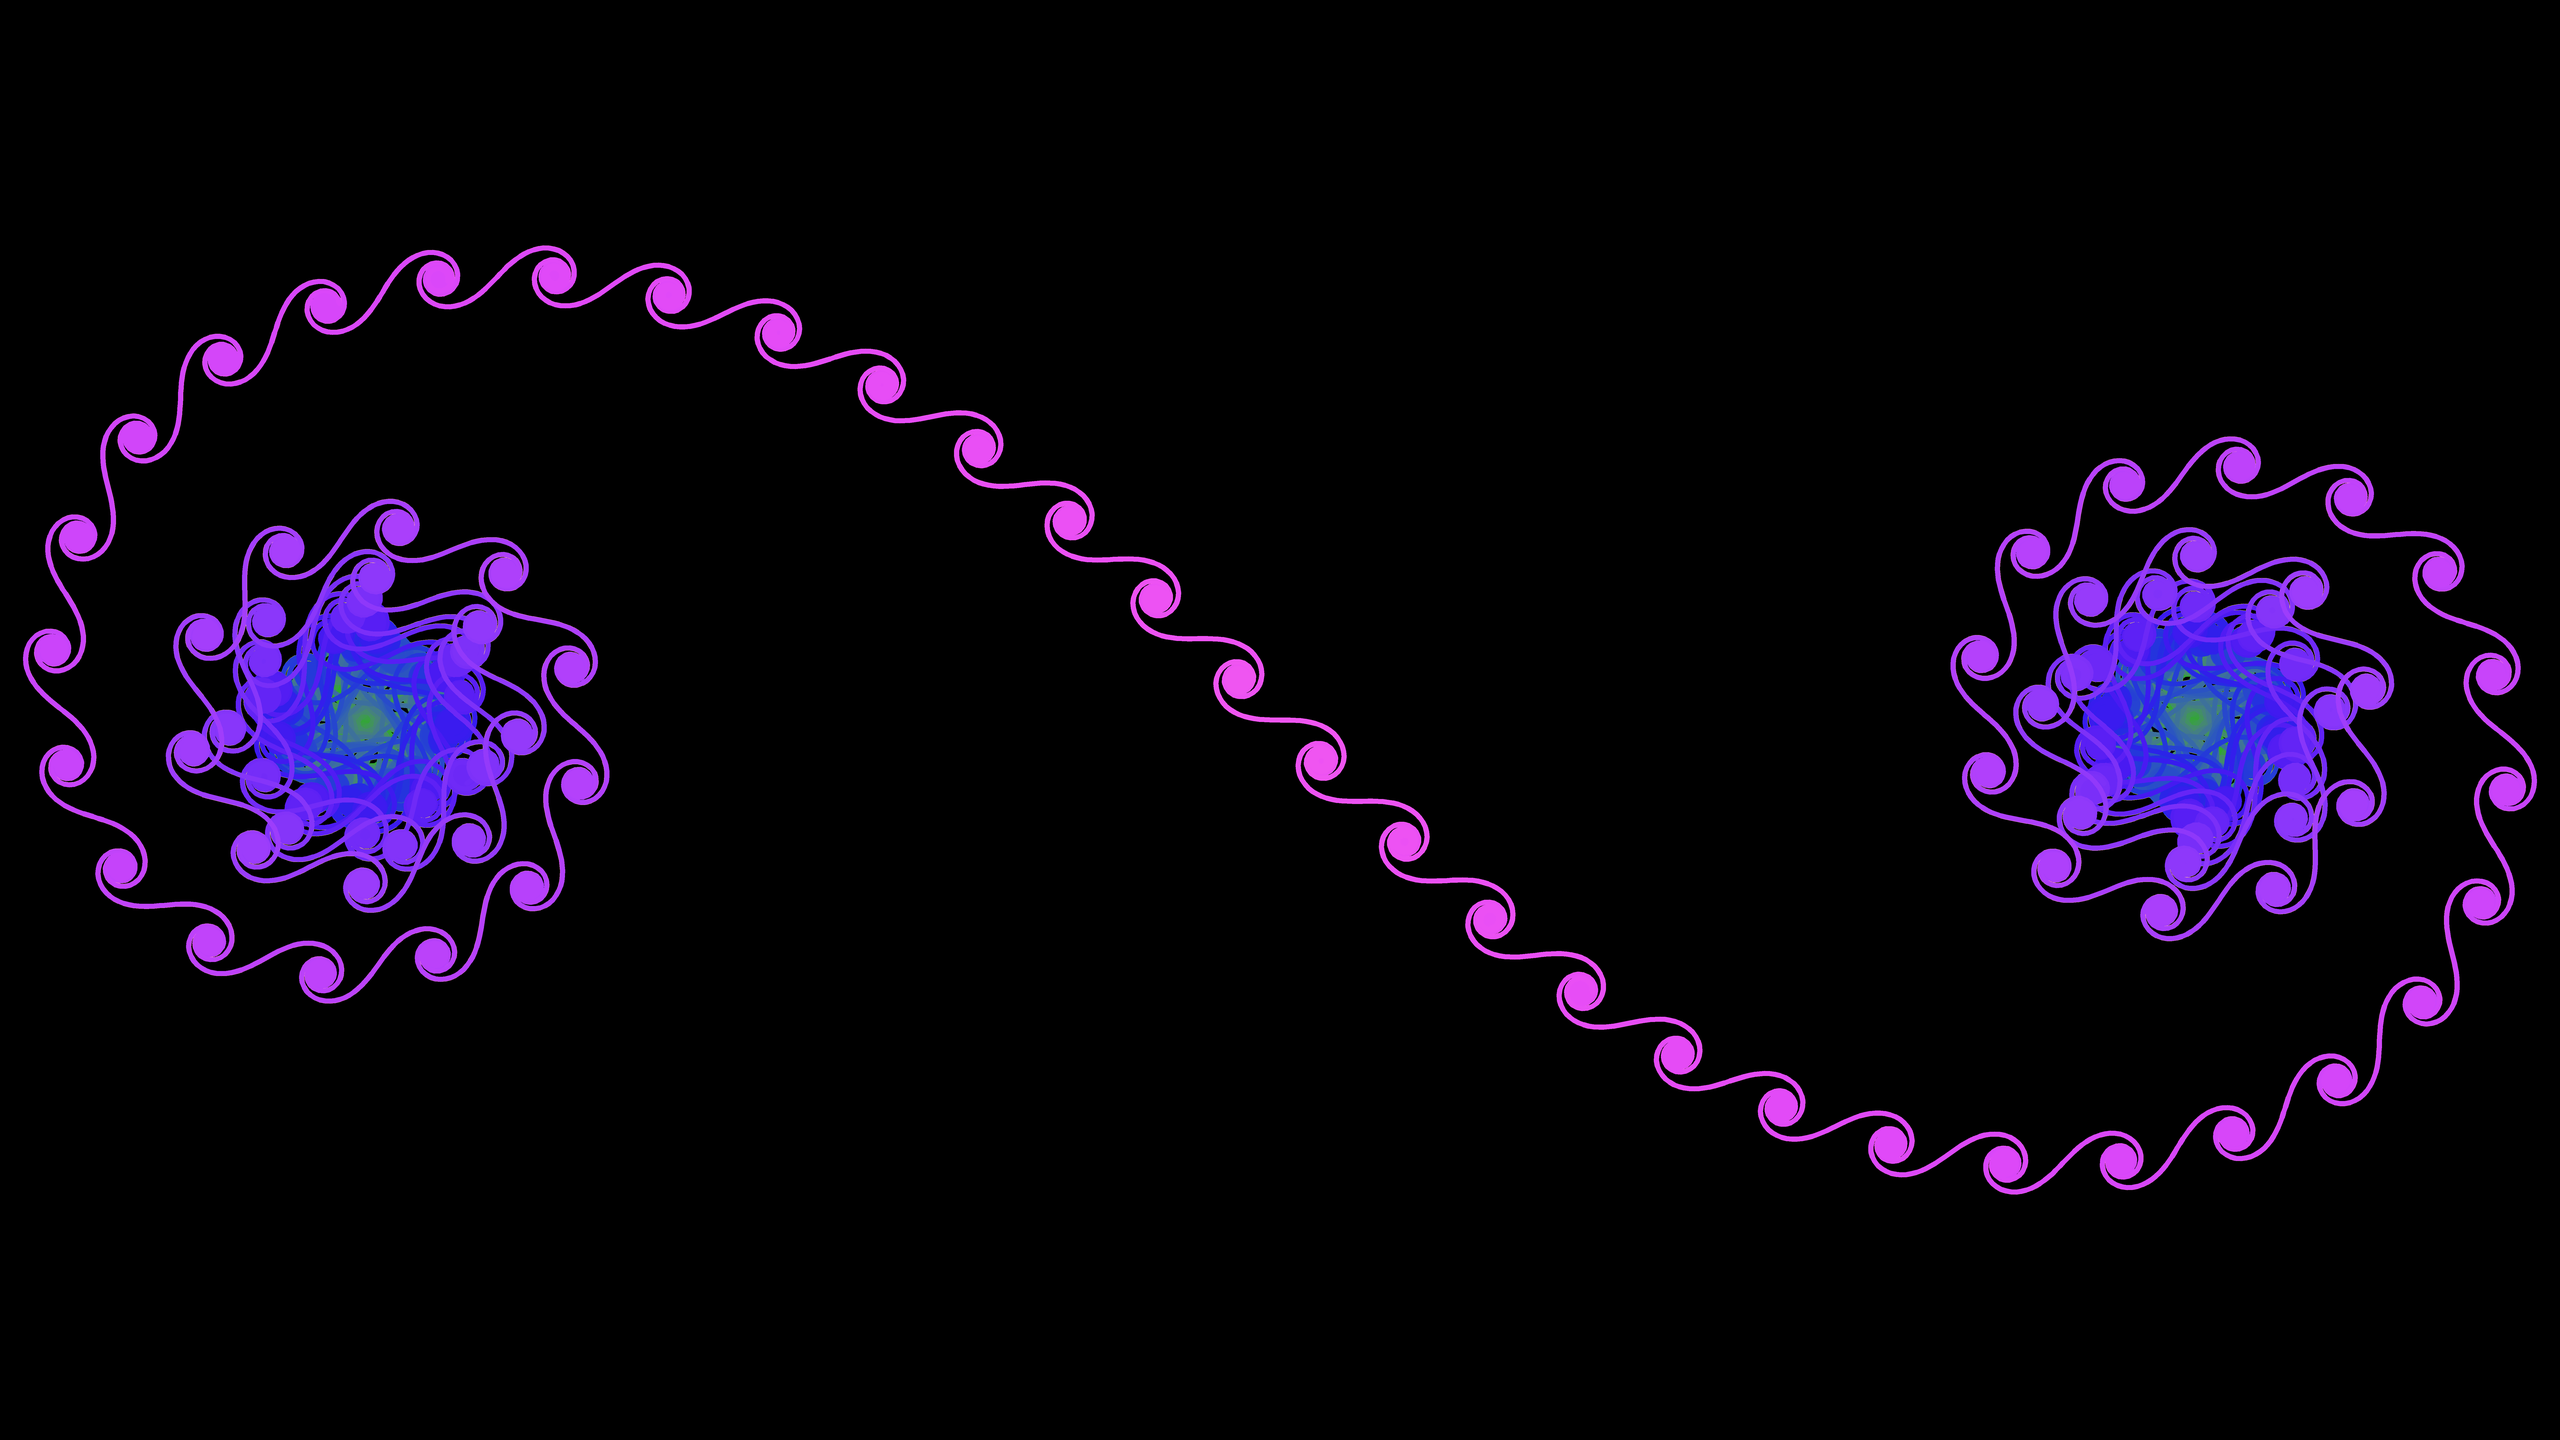
\includegraphics[width=0.3\textwidth]{./horizontal/tfa_046_p=249_q=124750_theta=0-71856_0_00_b_cyclic_mygbm_30_95_c78_Euler-Euler-Spiral_black.png}

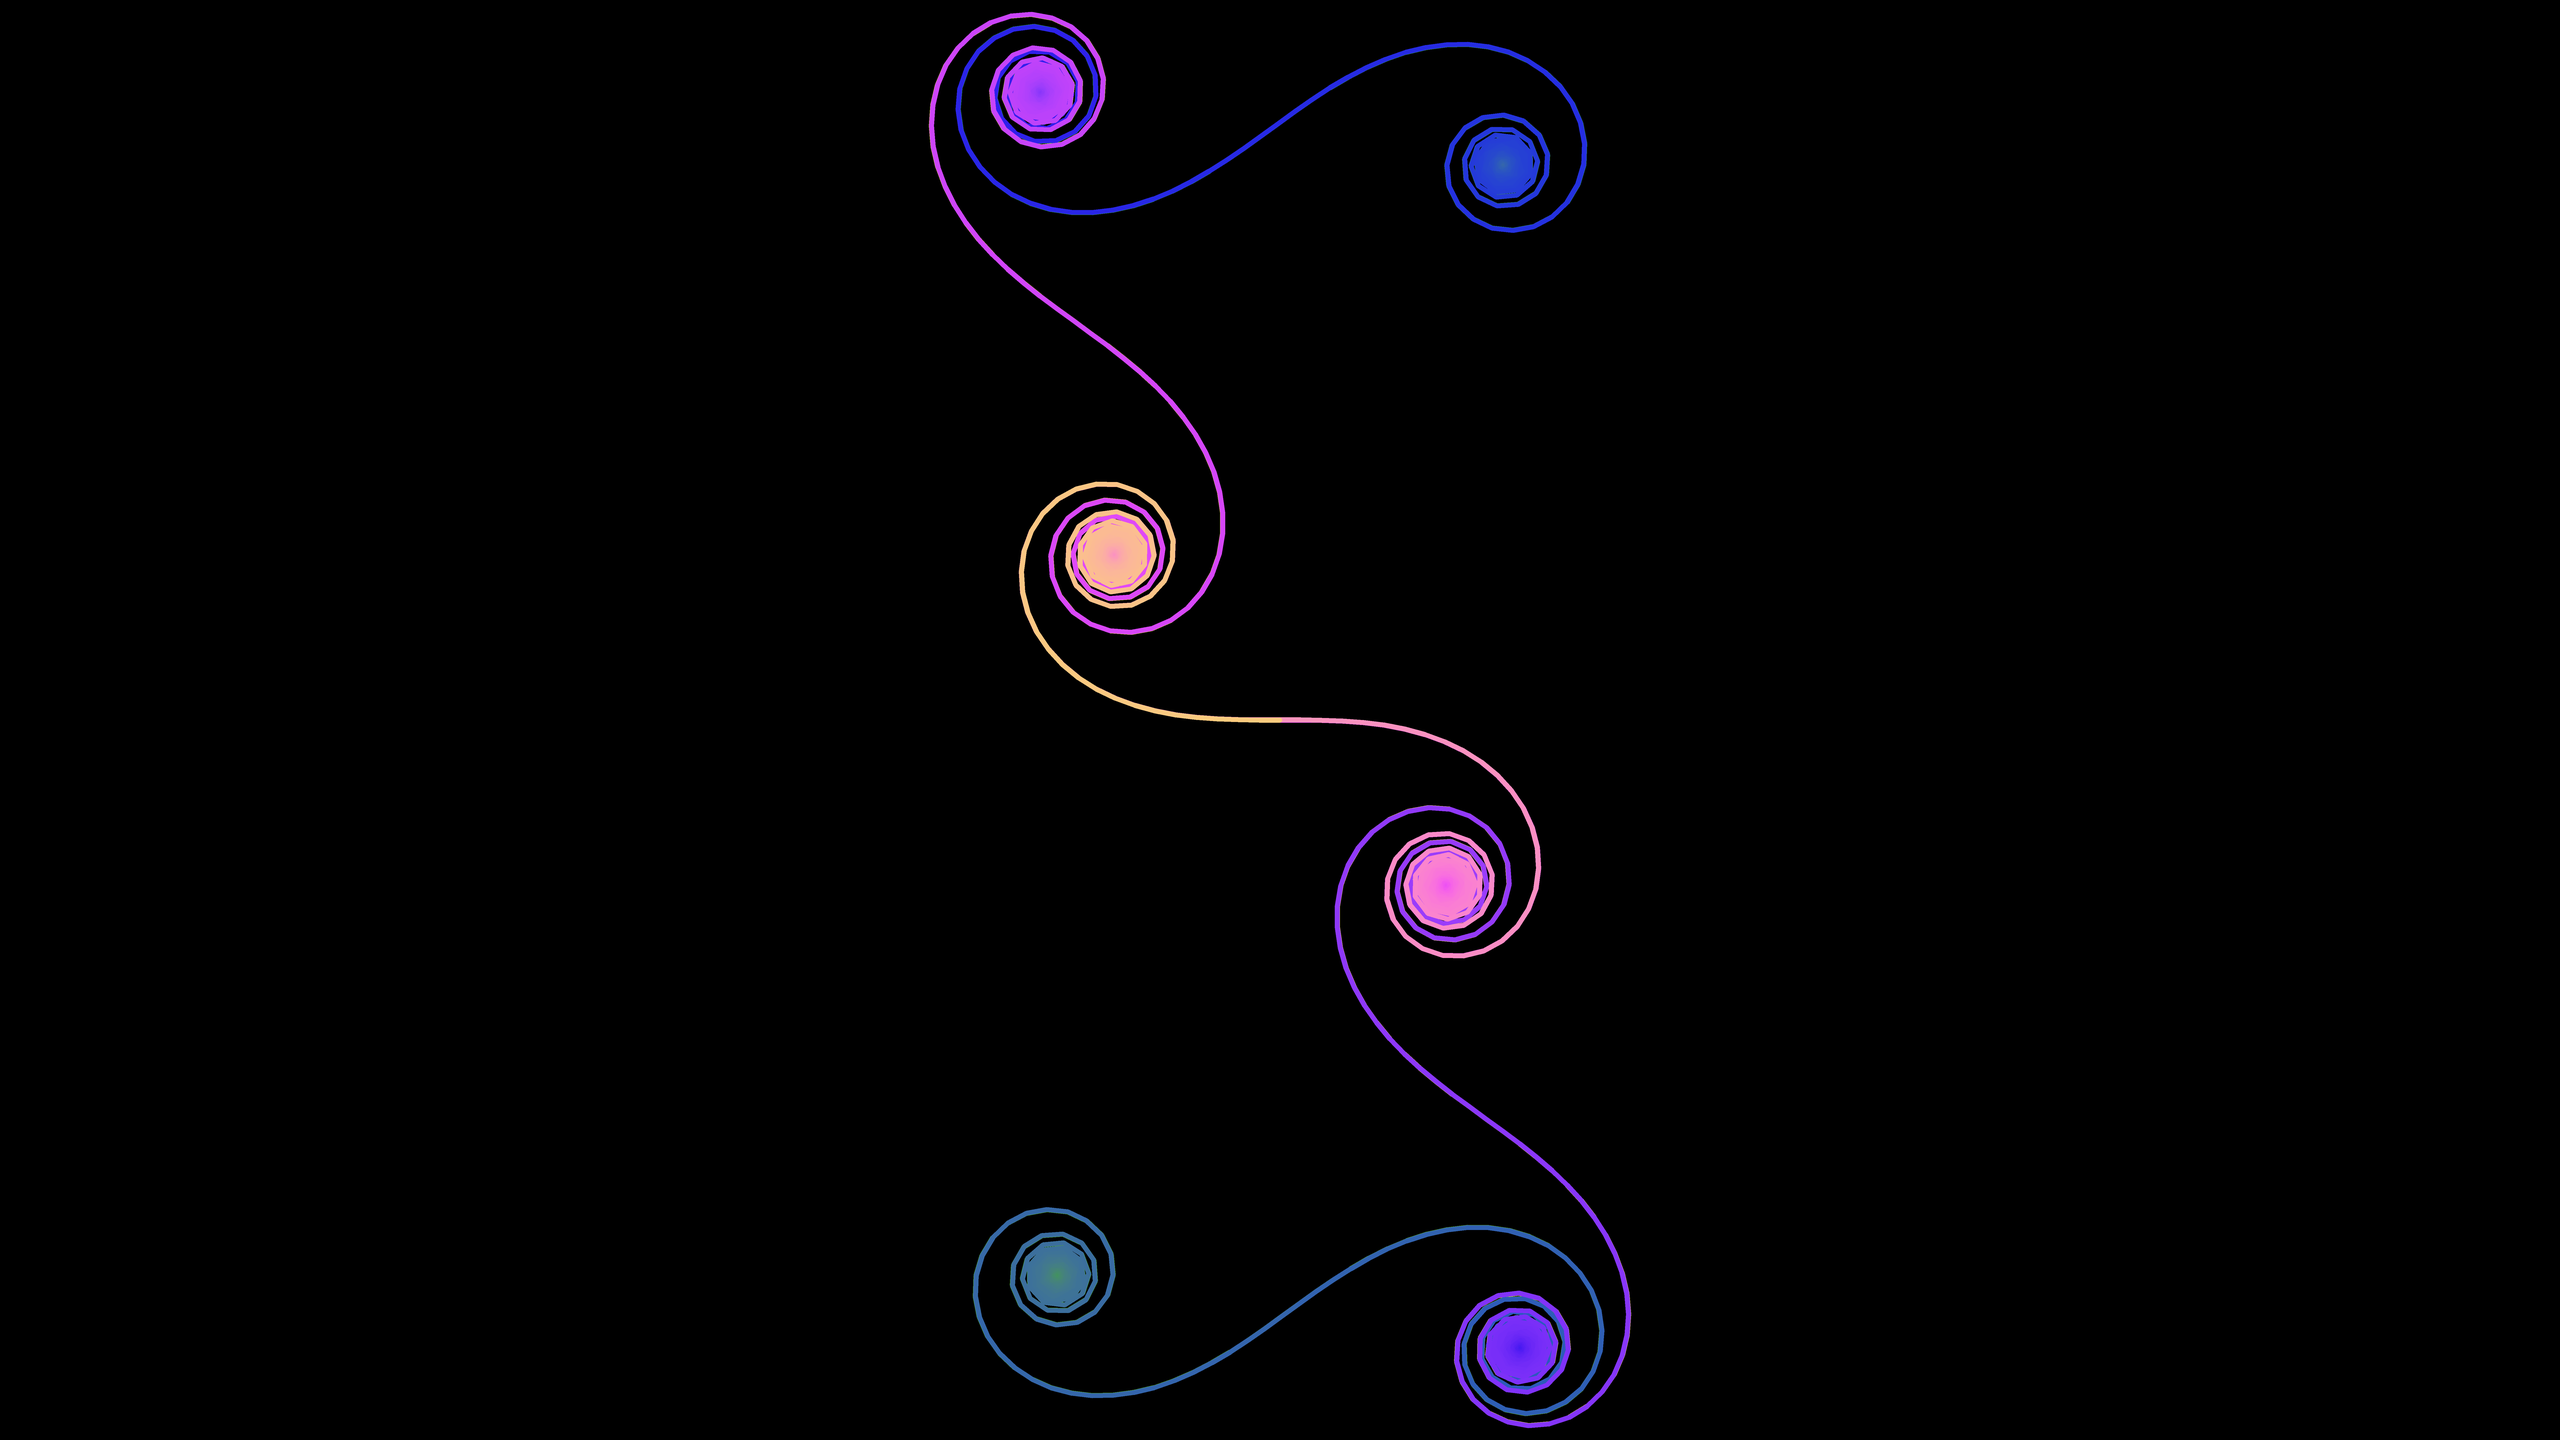
\includegraphics[width=0.3\textwidth]{./vertikal/tfa_046_p=005_q=2504_theta=0-71885_0_00_b_cyclic_mygbm_30_95_c78_Euler-Euler-Spiral_black.png}
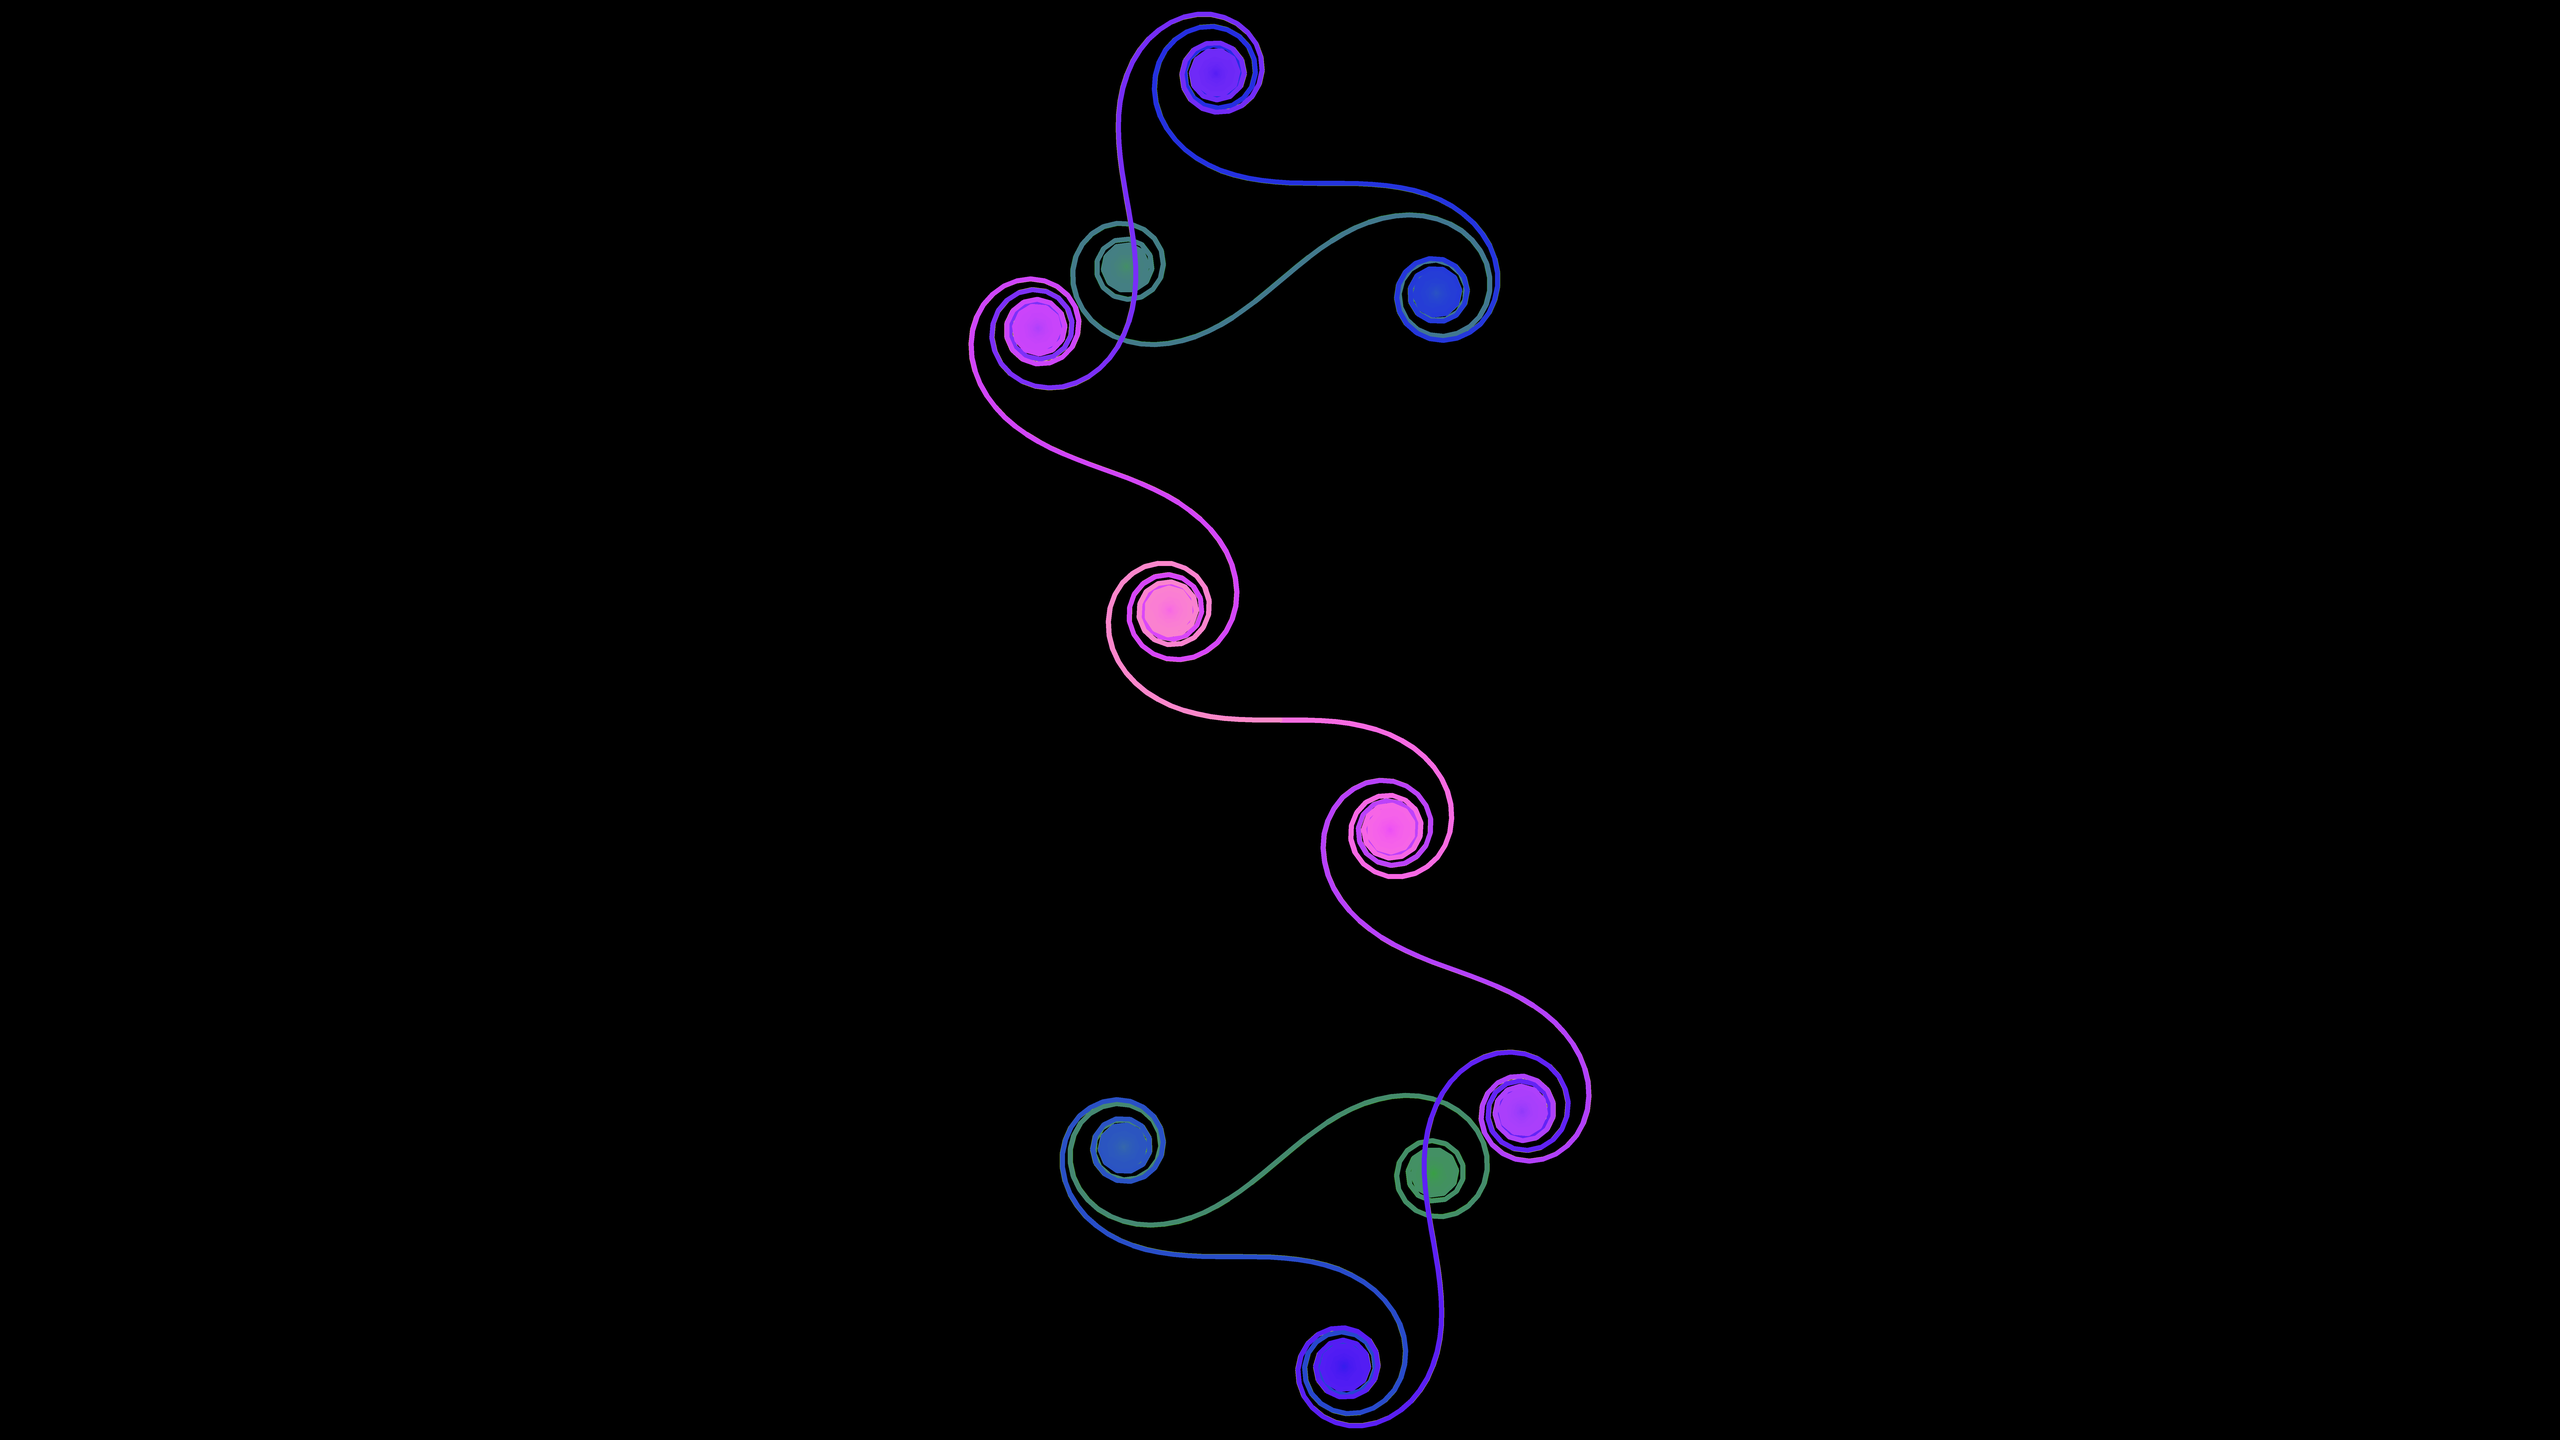
\includegraphics[width=0.3\textwidth]{./vertikal/tfa_046_p=009_q=4508_theta=0-71872_0_00_b_cyclic_mygbm_30_95_c78_Euler-Euler-Spiral_black.png}
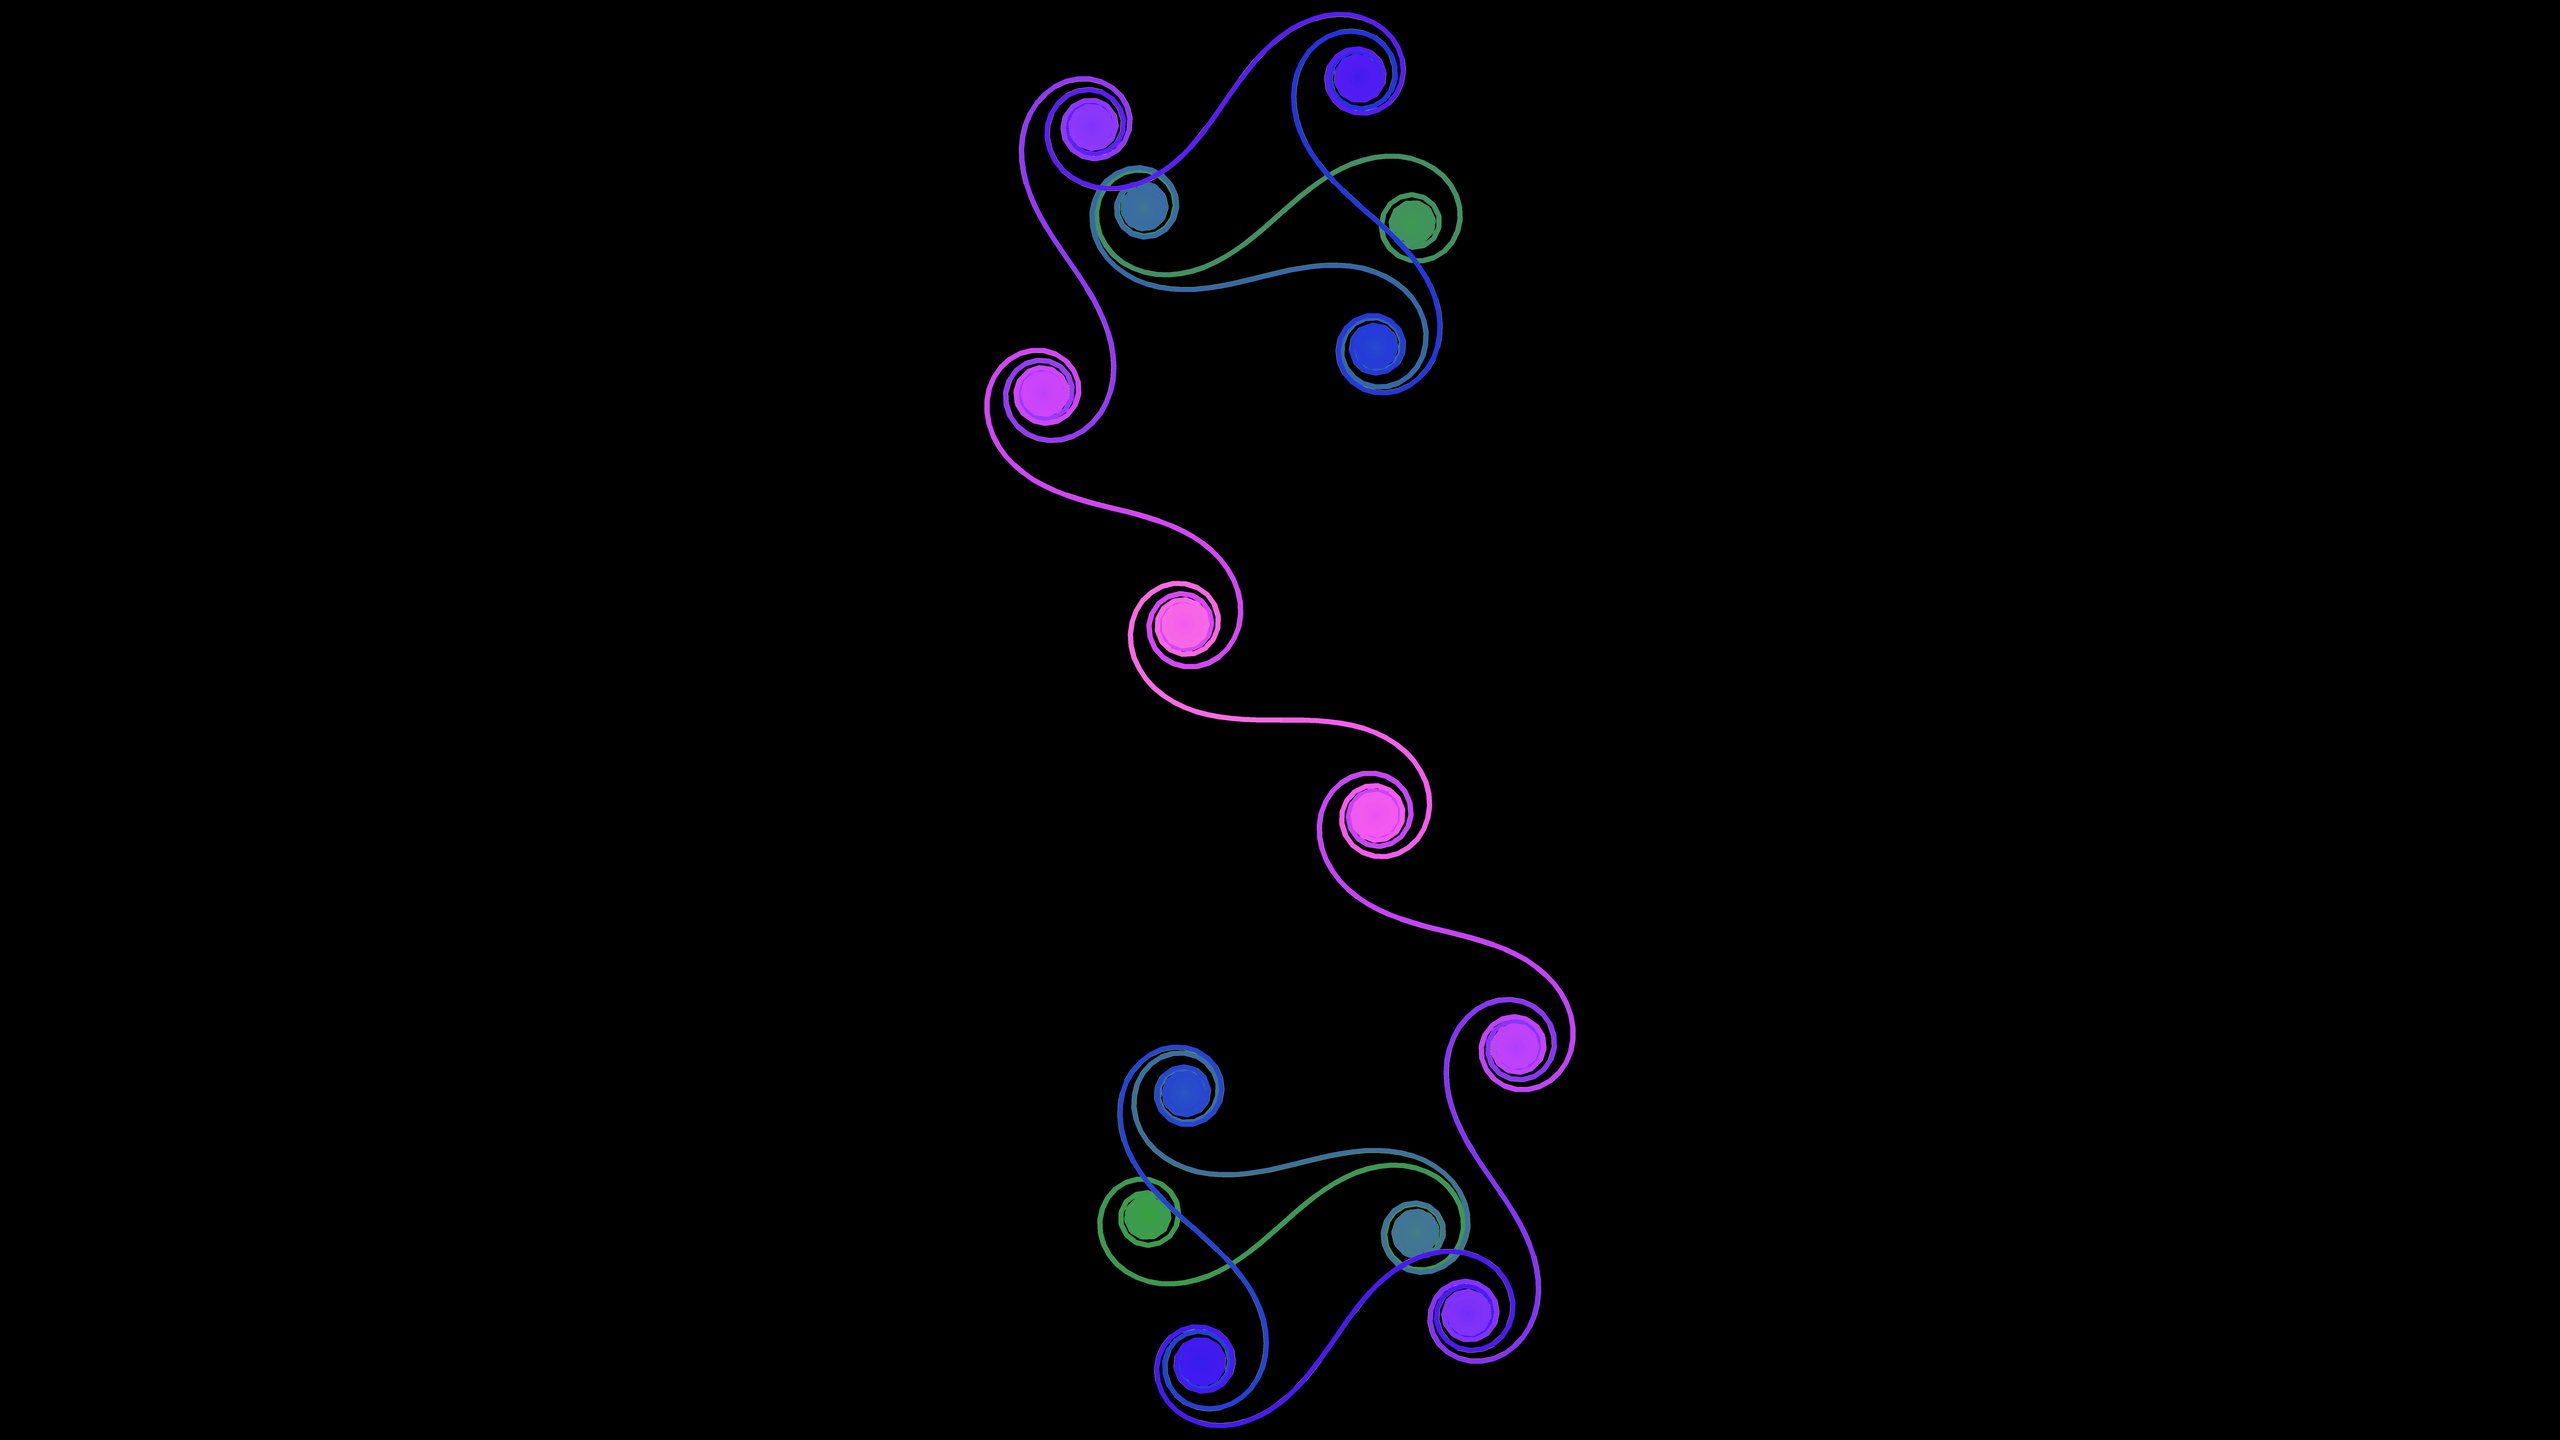
\includegraphics[width=0.3\textwidth]{./vertikal/tfa_046_p=013_q=6512_theta=0-71867_0_00_b_cyclic_mygbm_30_95_c78_Euler-Euler-Spiral_black.png}

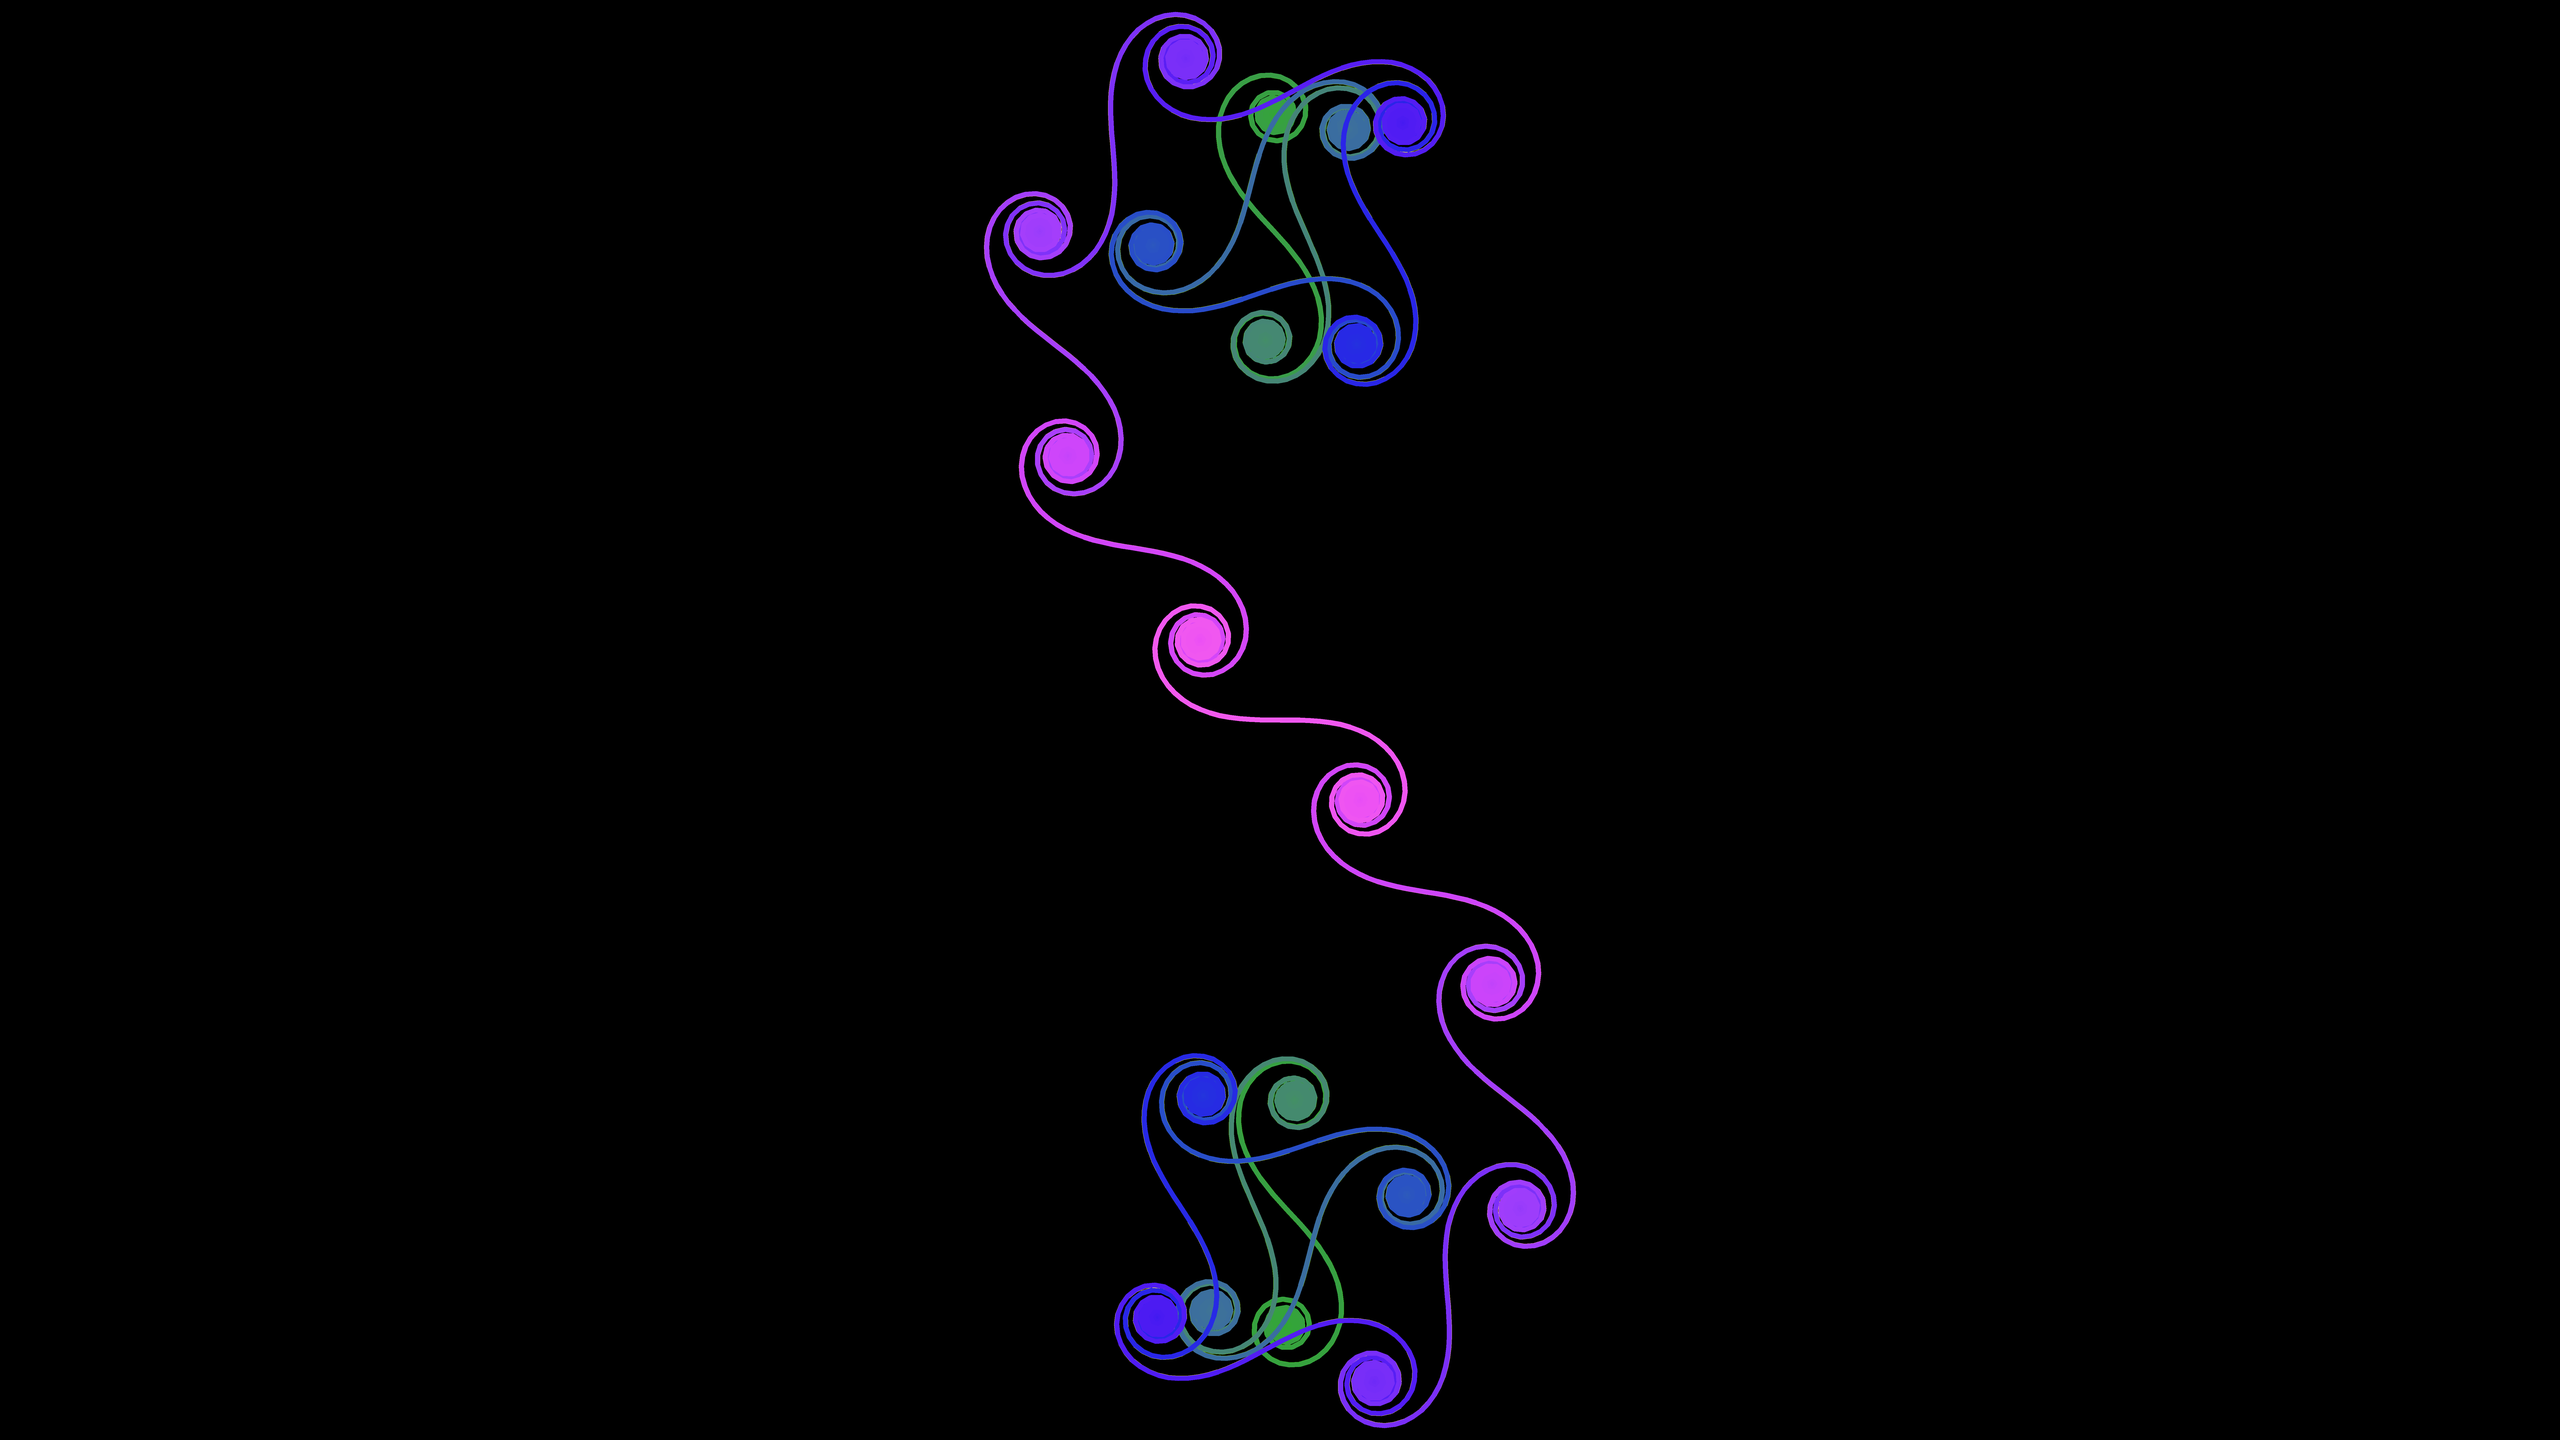
\includegraphics[width=0.3\textwidth]{./vertikal/tfa_046_p=019_q=9518_theta=0-71864_0_00_b_cyclic_mygbm_30_95_c78_Euler-Euler-Spiral_black.png}
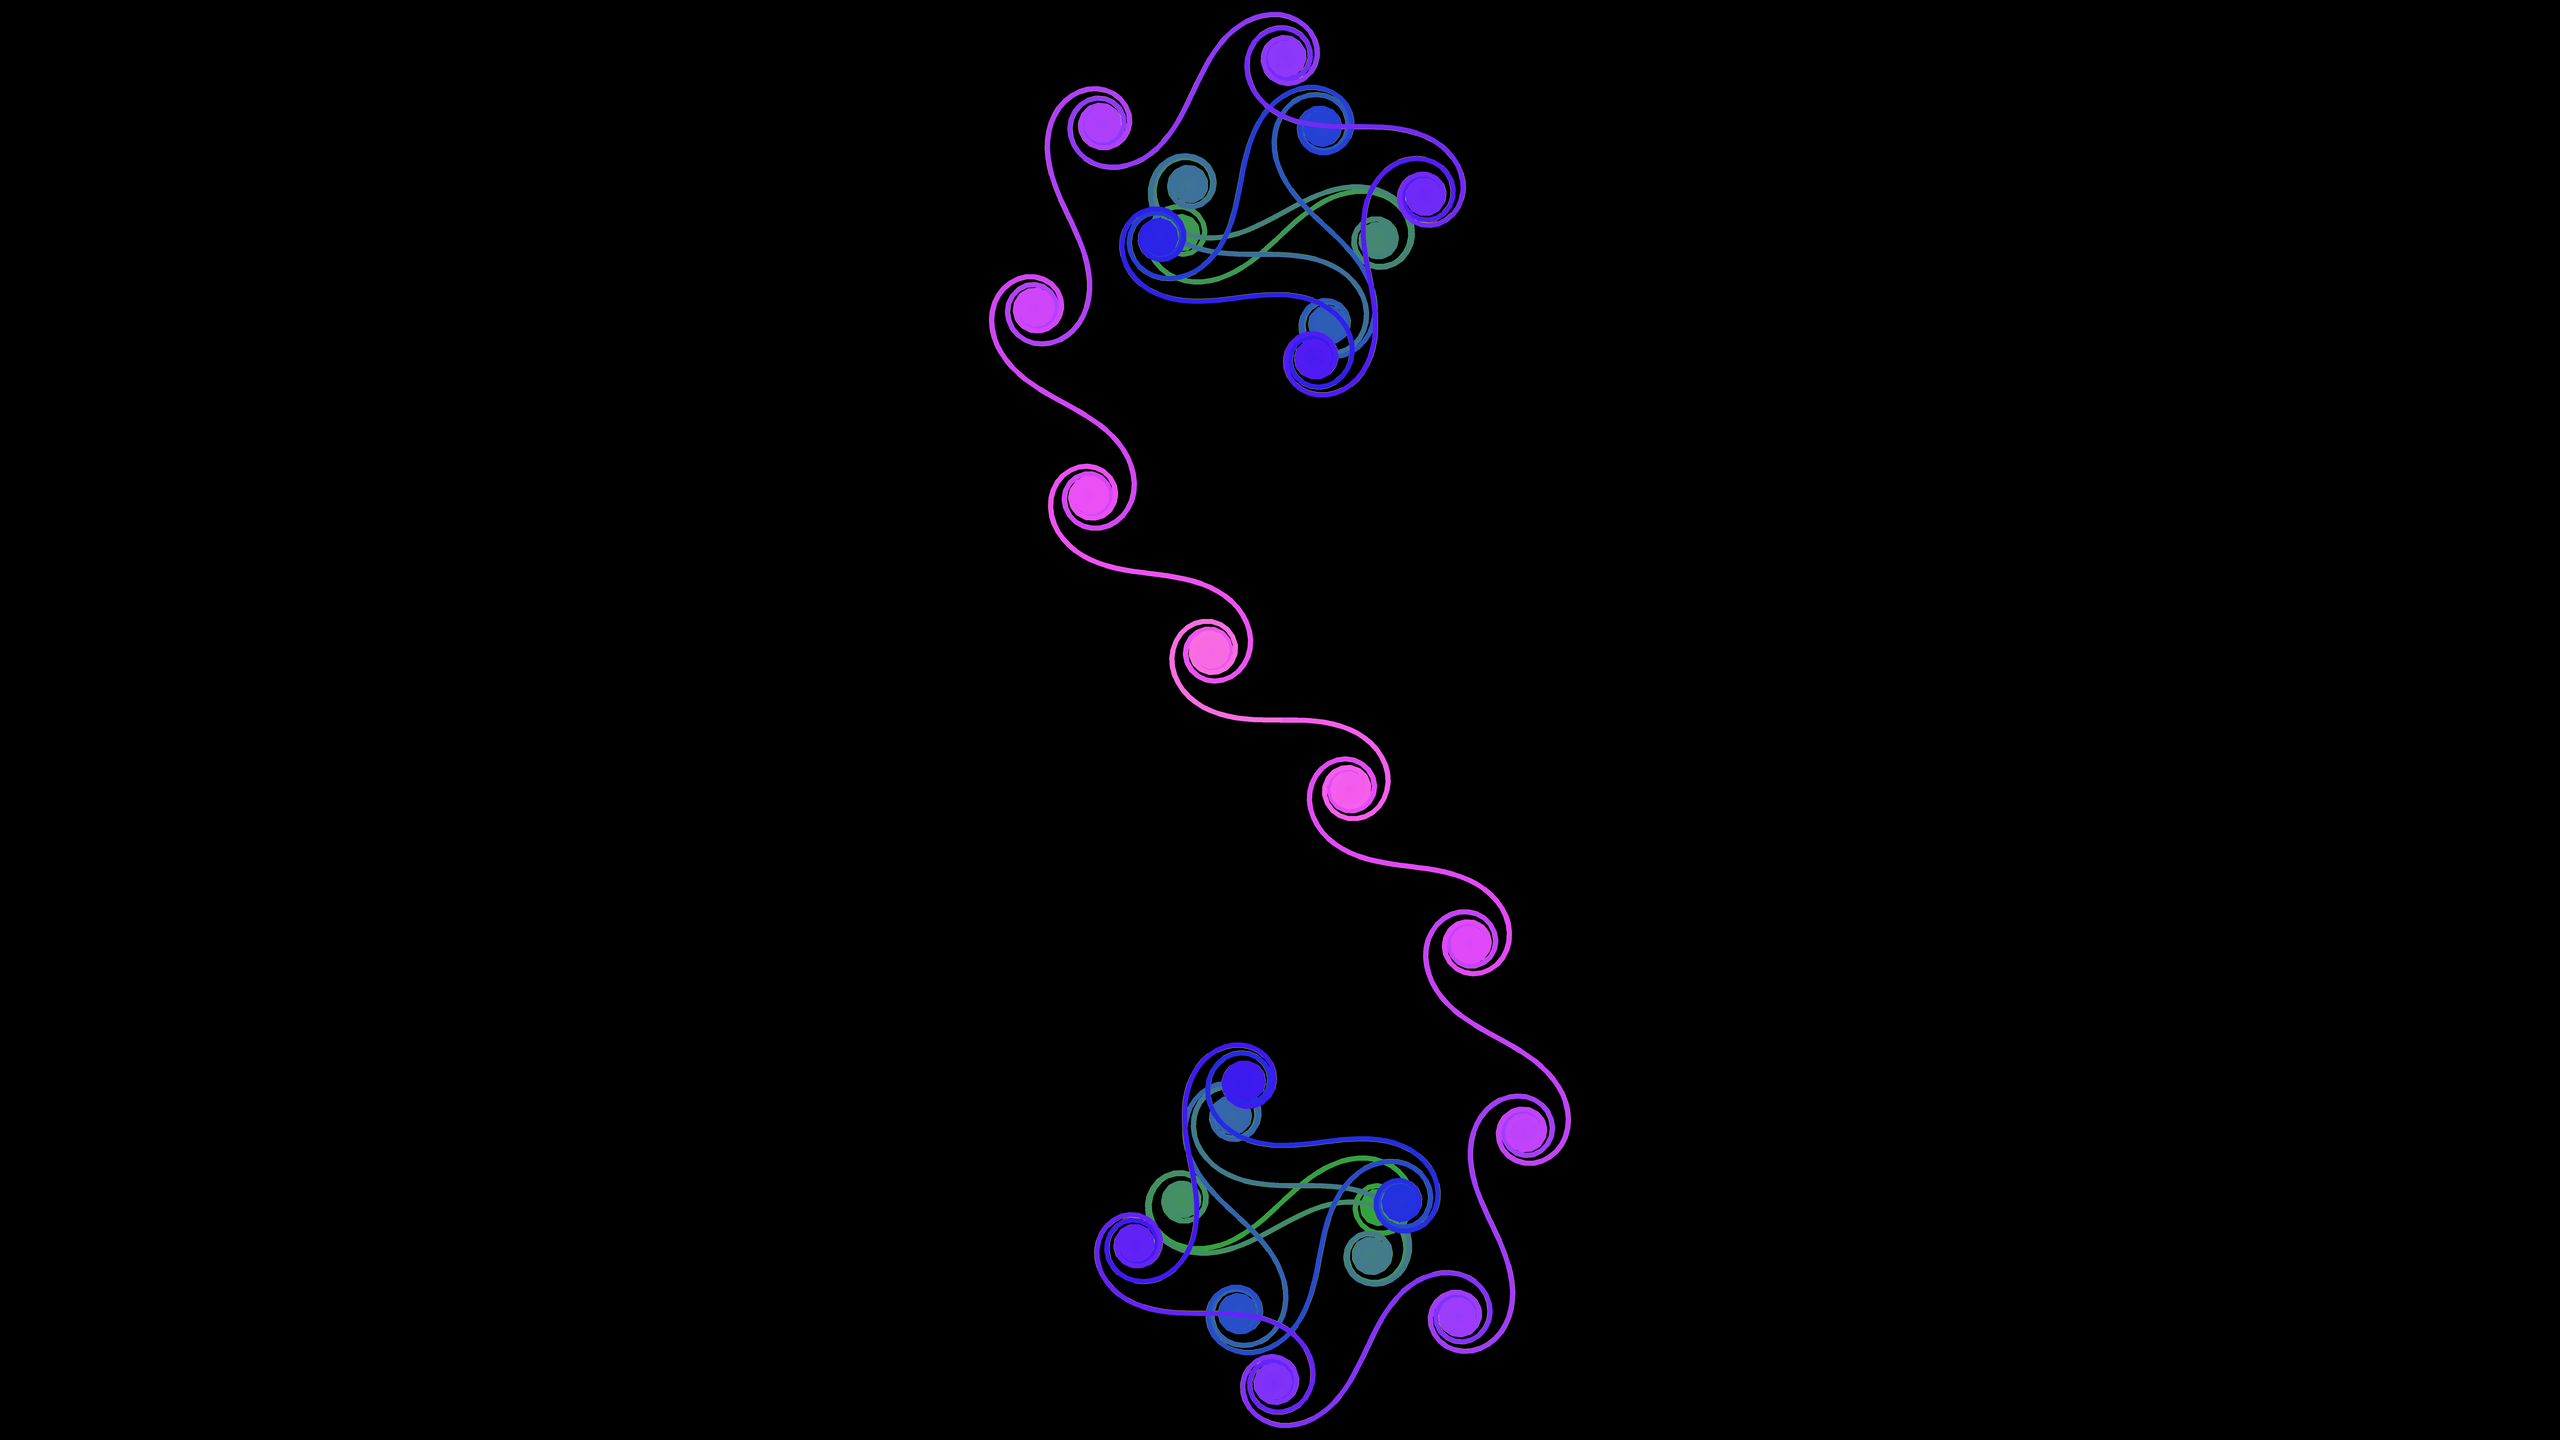
\includegraphics[width=0.3\textwidth]{./vertikal/tfa_046_p=025_q=12524_theta=0-71862_0_00_b_cyclic_mygbm_30_95_c78_Euler-Euler-Spiral_black.png}
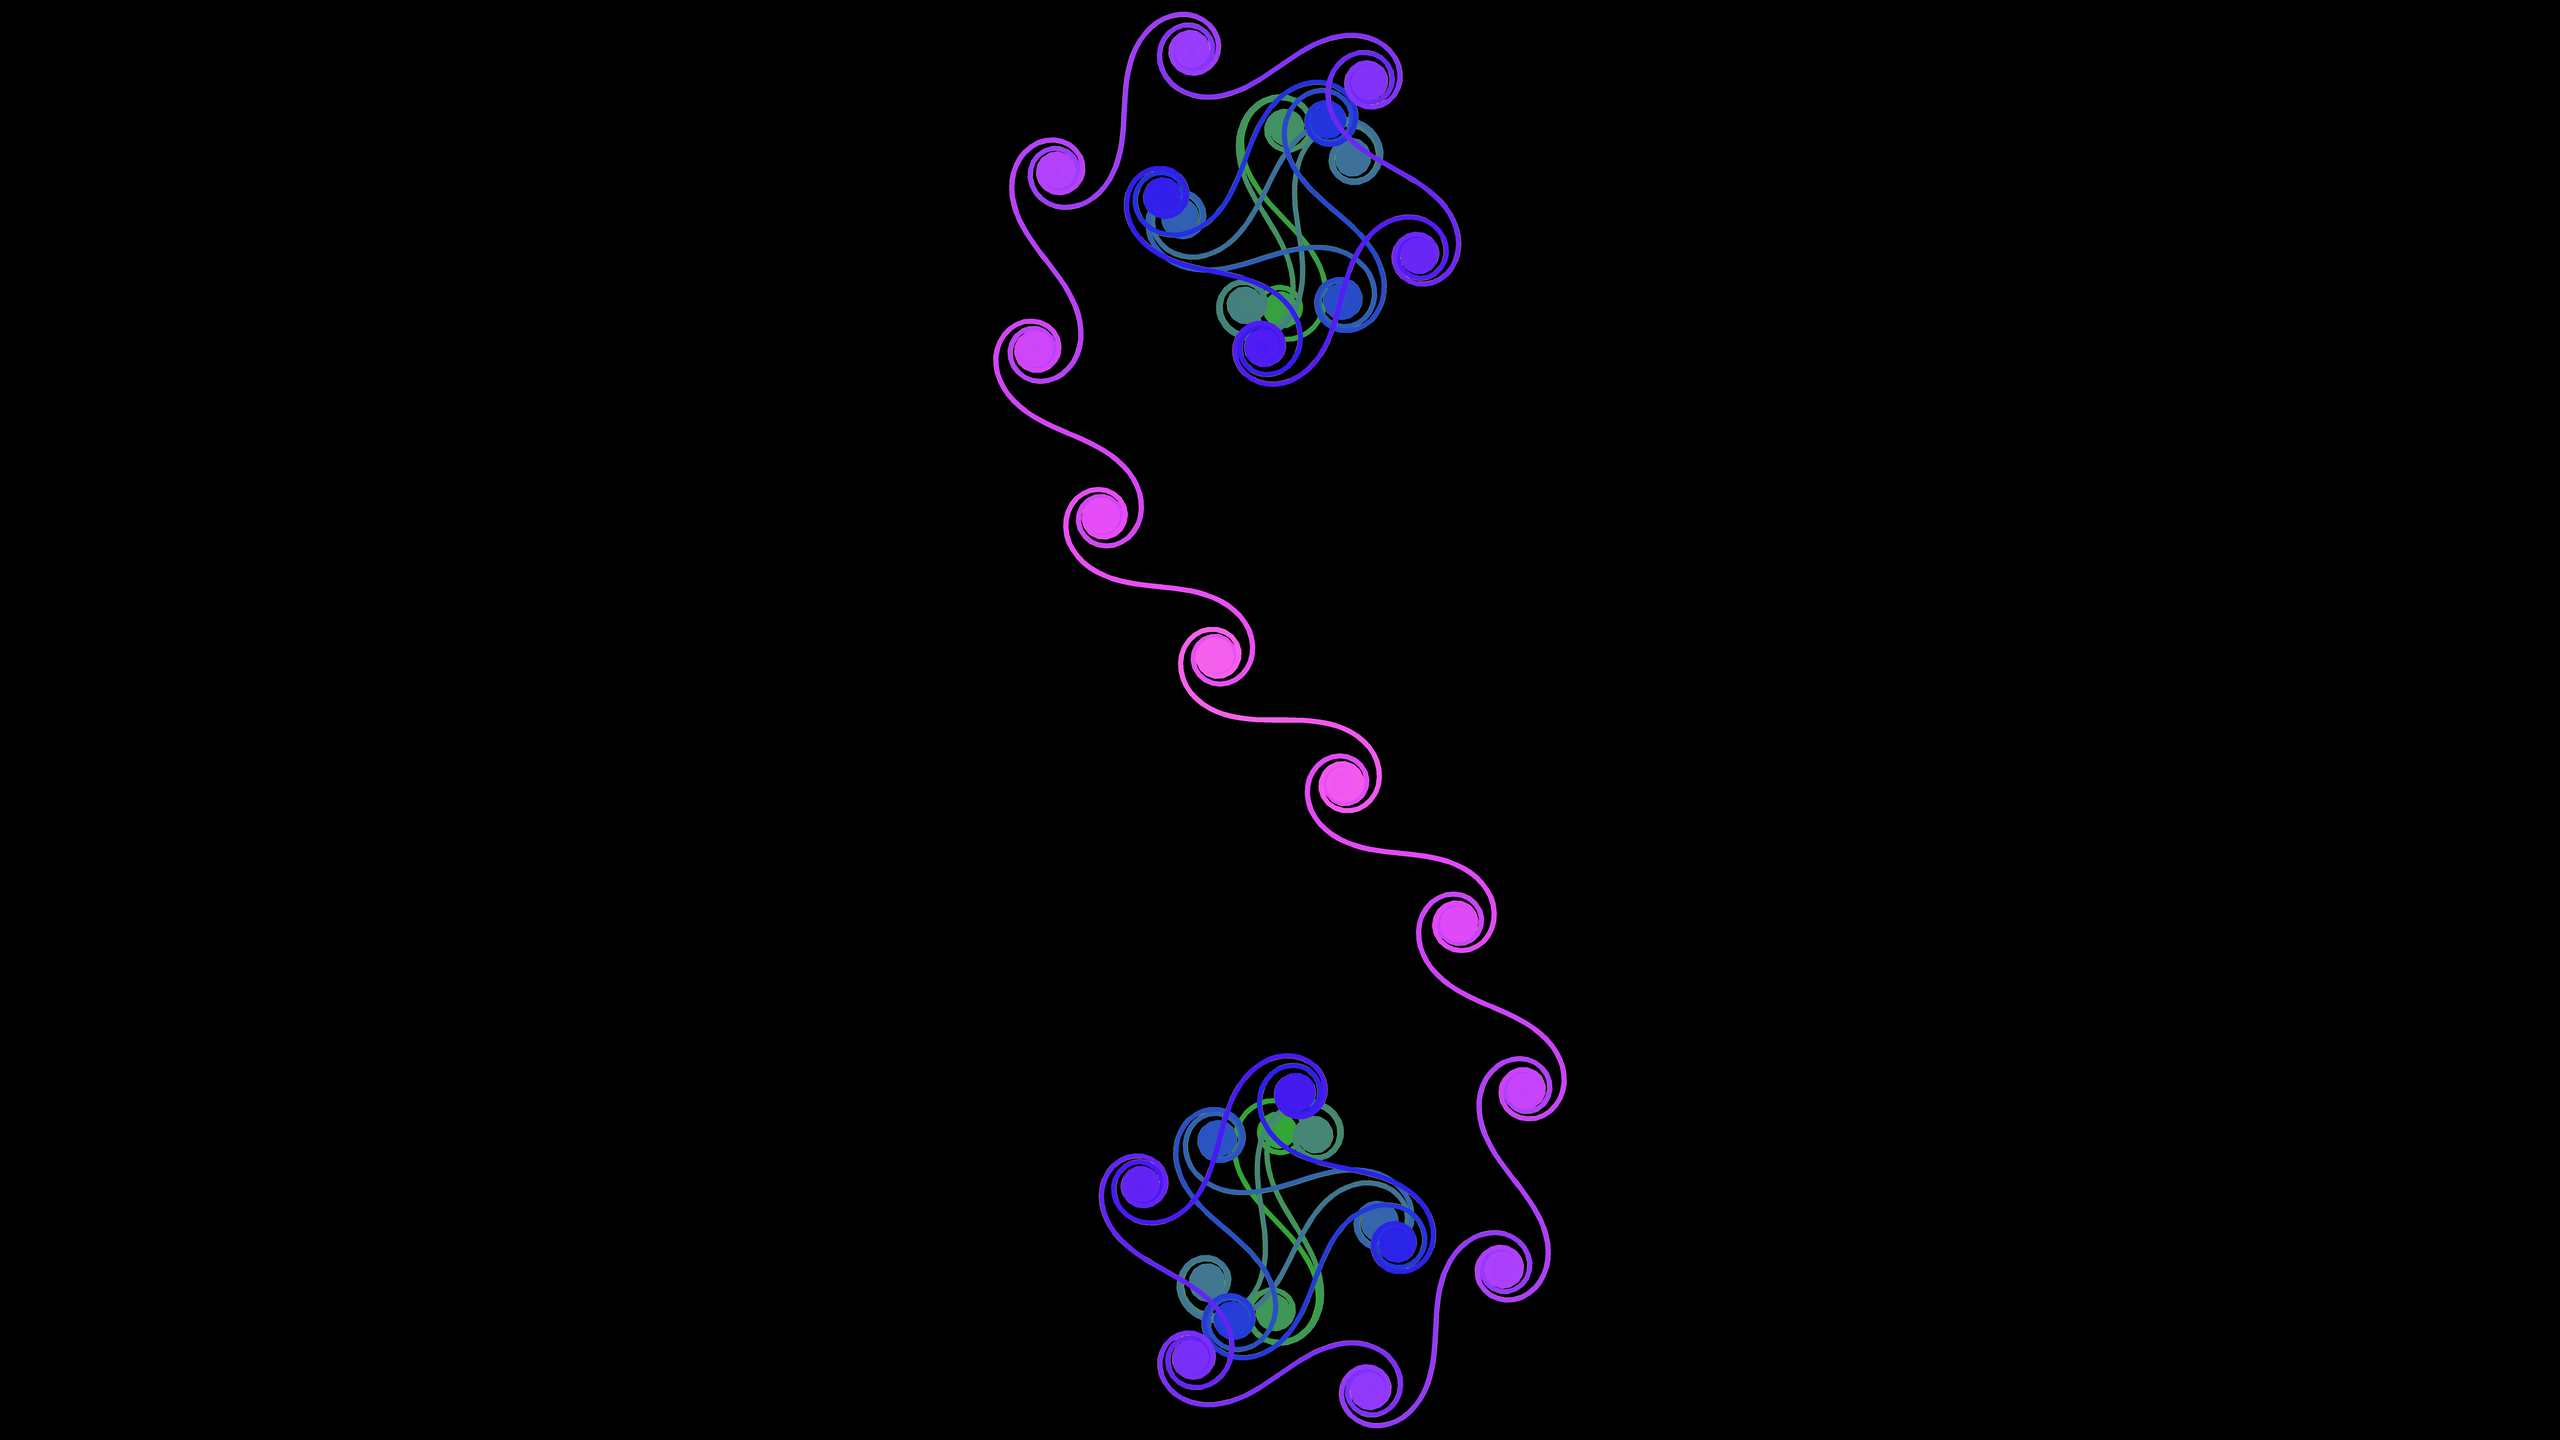
\includegraphics[width=0.3\textwidth]{./vertikal/tfa_046_p=031_q=15530_theta=0-71861_0_00_b_cyclic_mygbm_30_95_c78_Euler-Euler-Spiral_black.png}

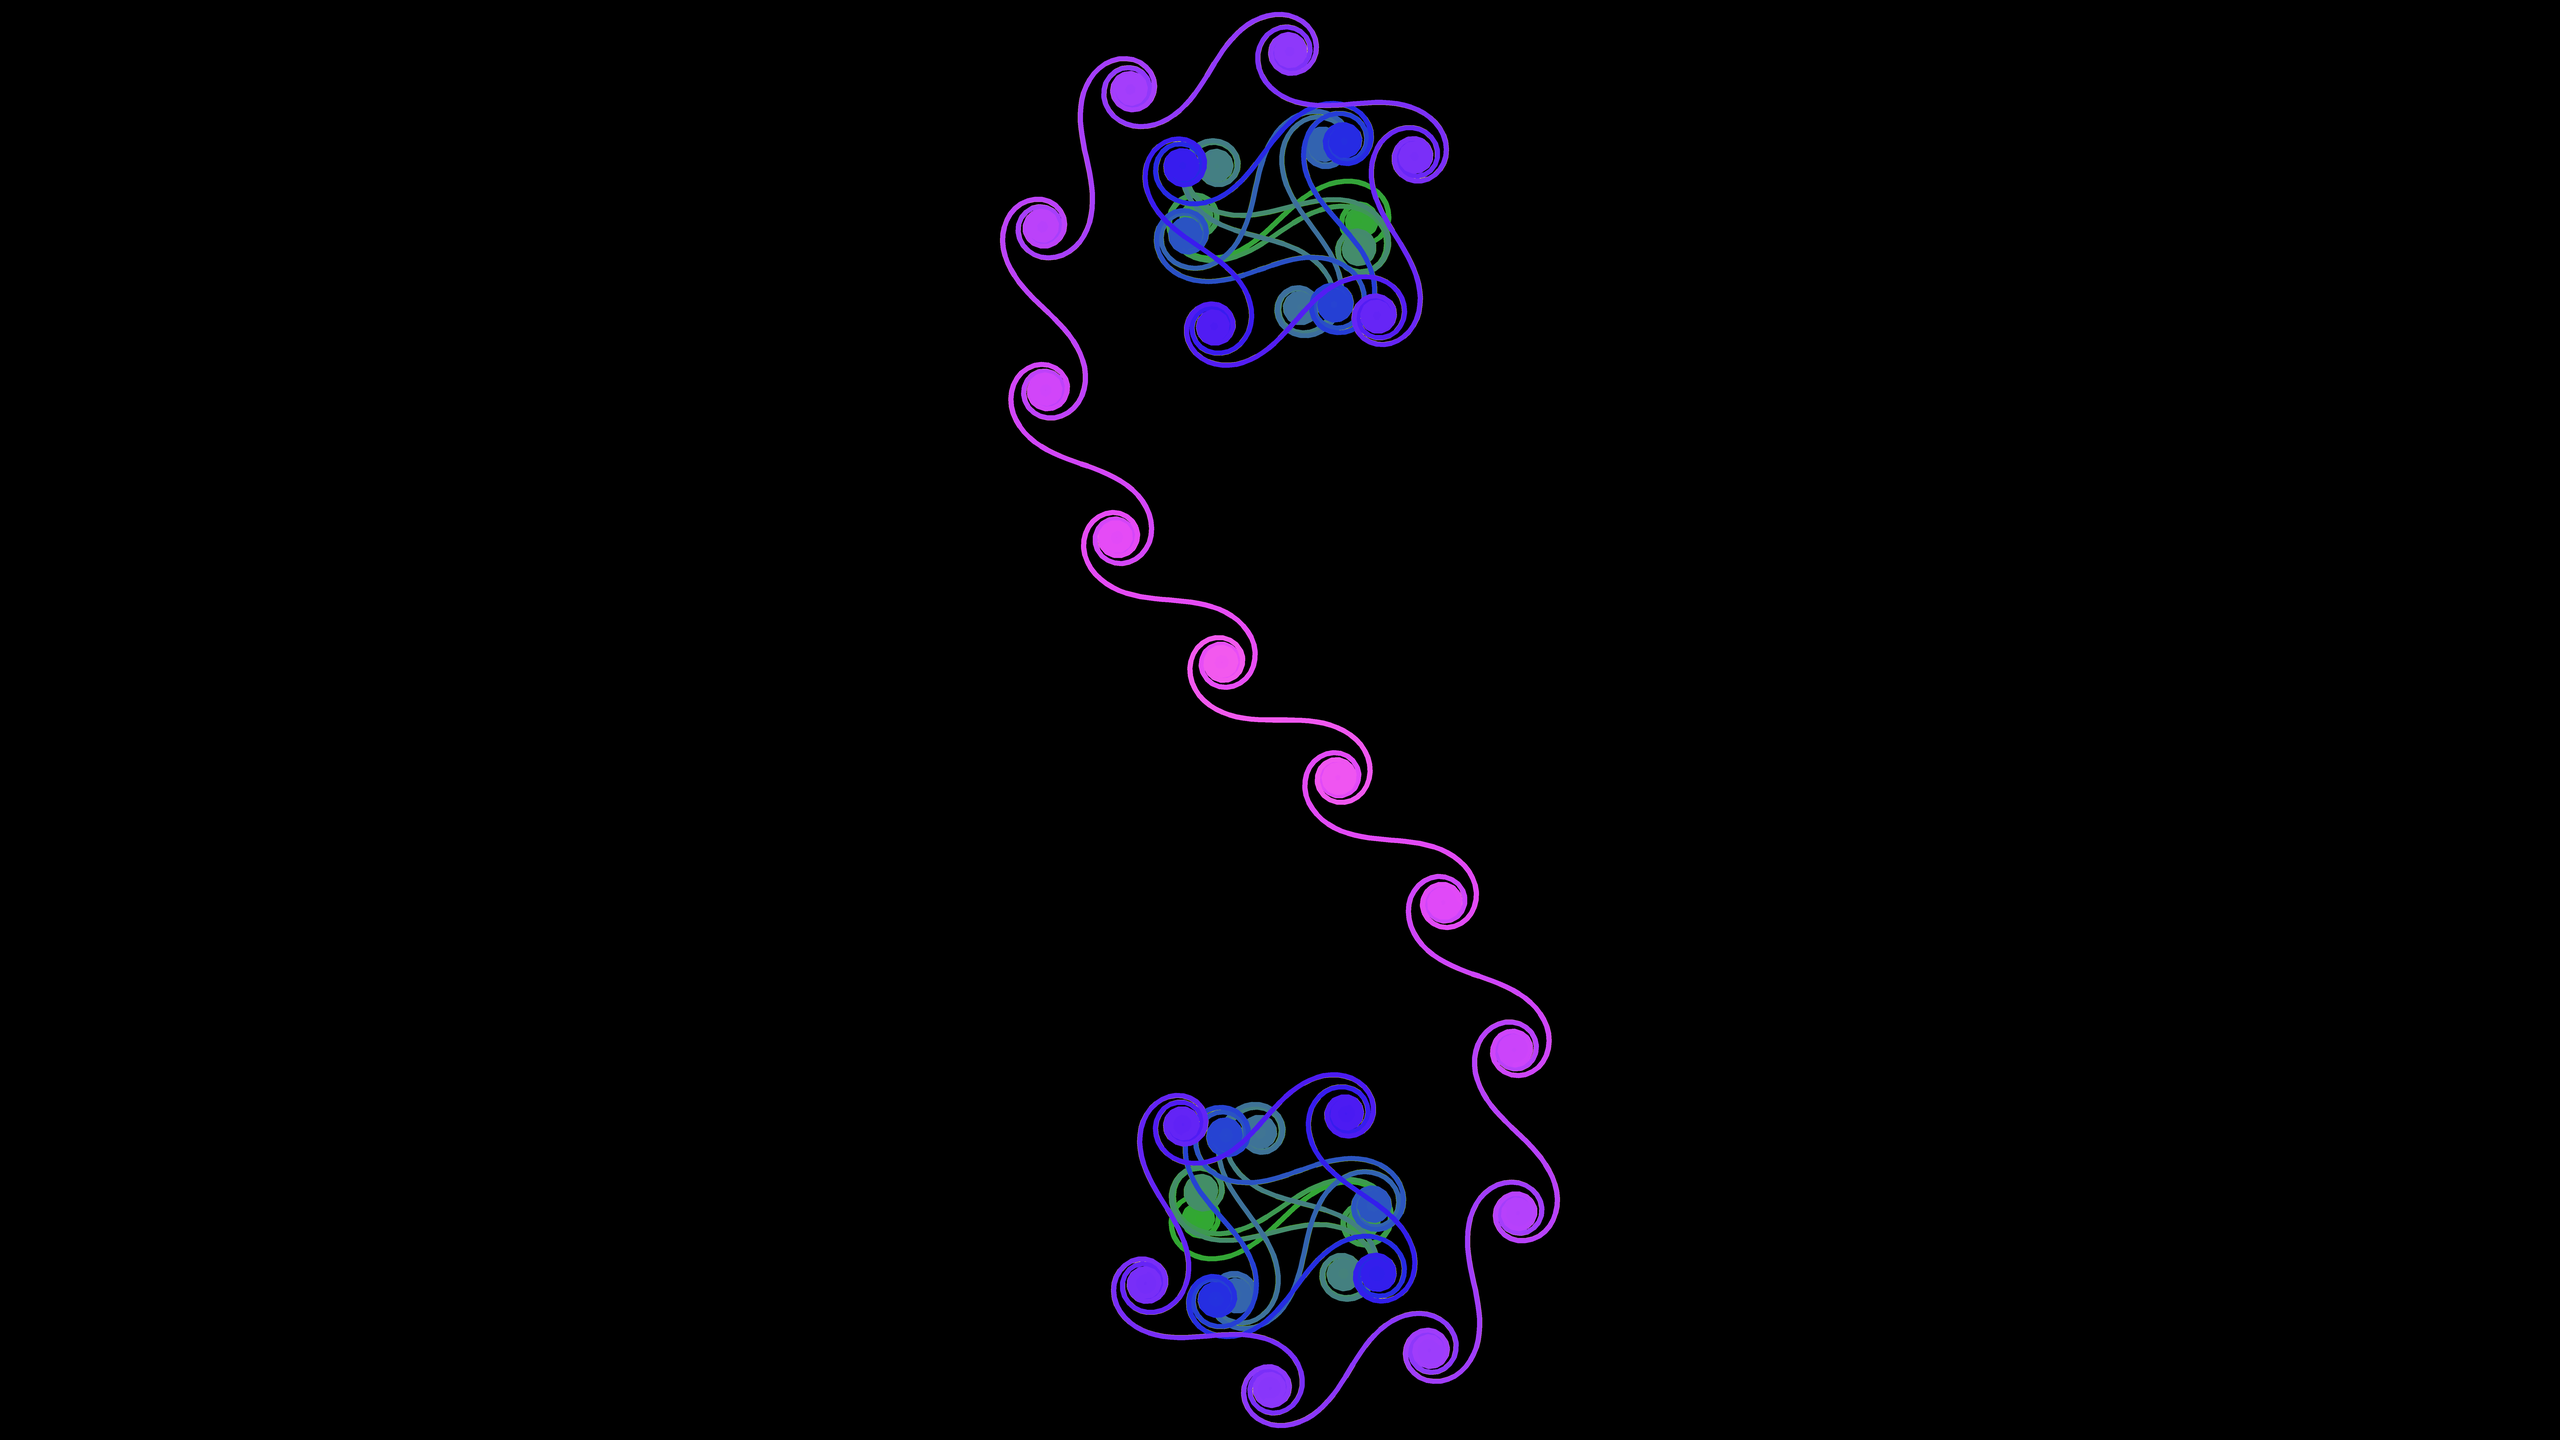
\includegraphics[width=0.3\textwidth]{./vertikal/tfa_046_p=037_q=18536_theta=0-71860_0_00_b_cyclic_mygbm_30_95_c78_Euler-Euler-Spiral_black.png}
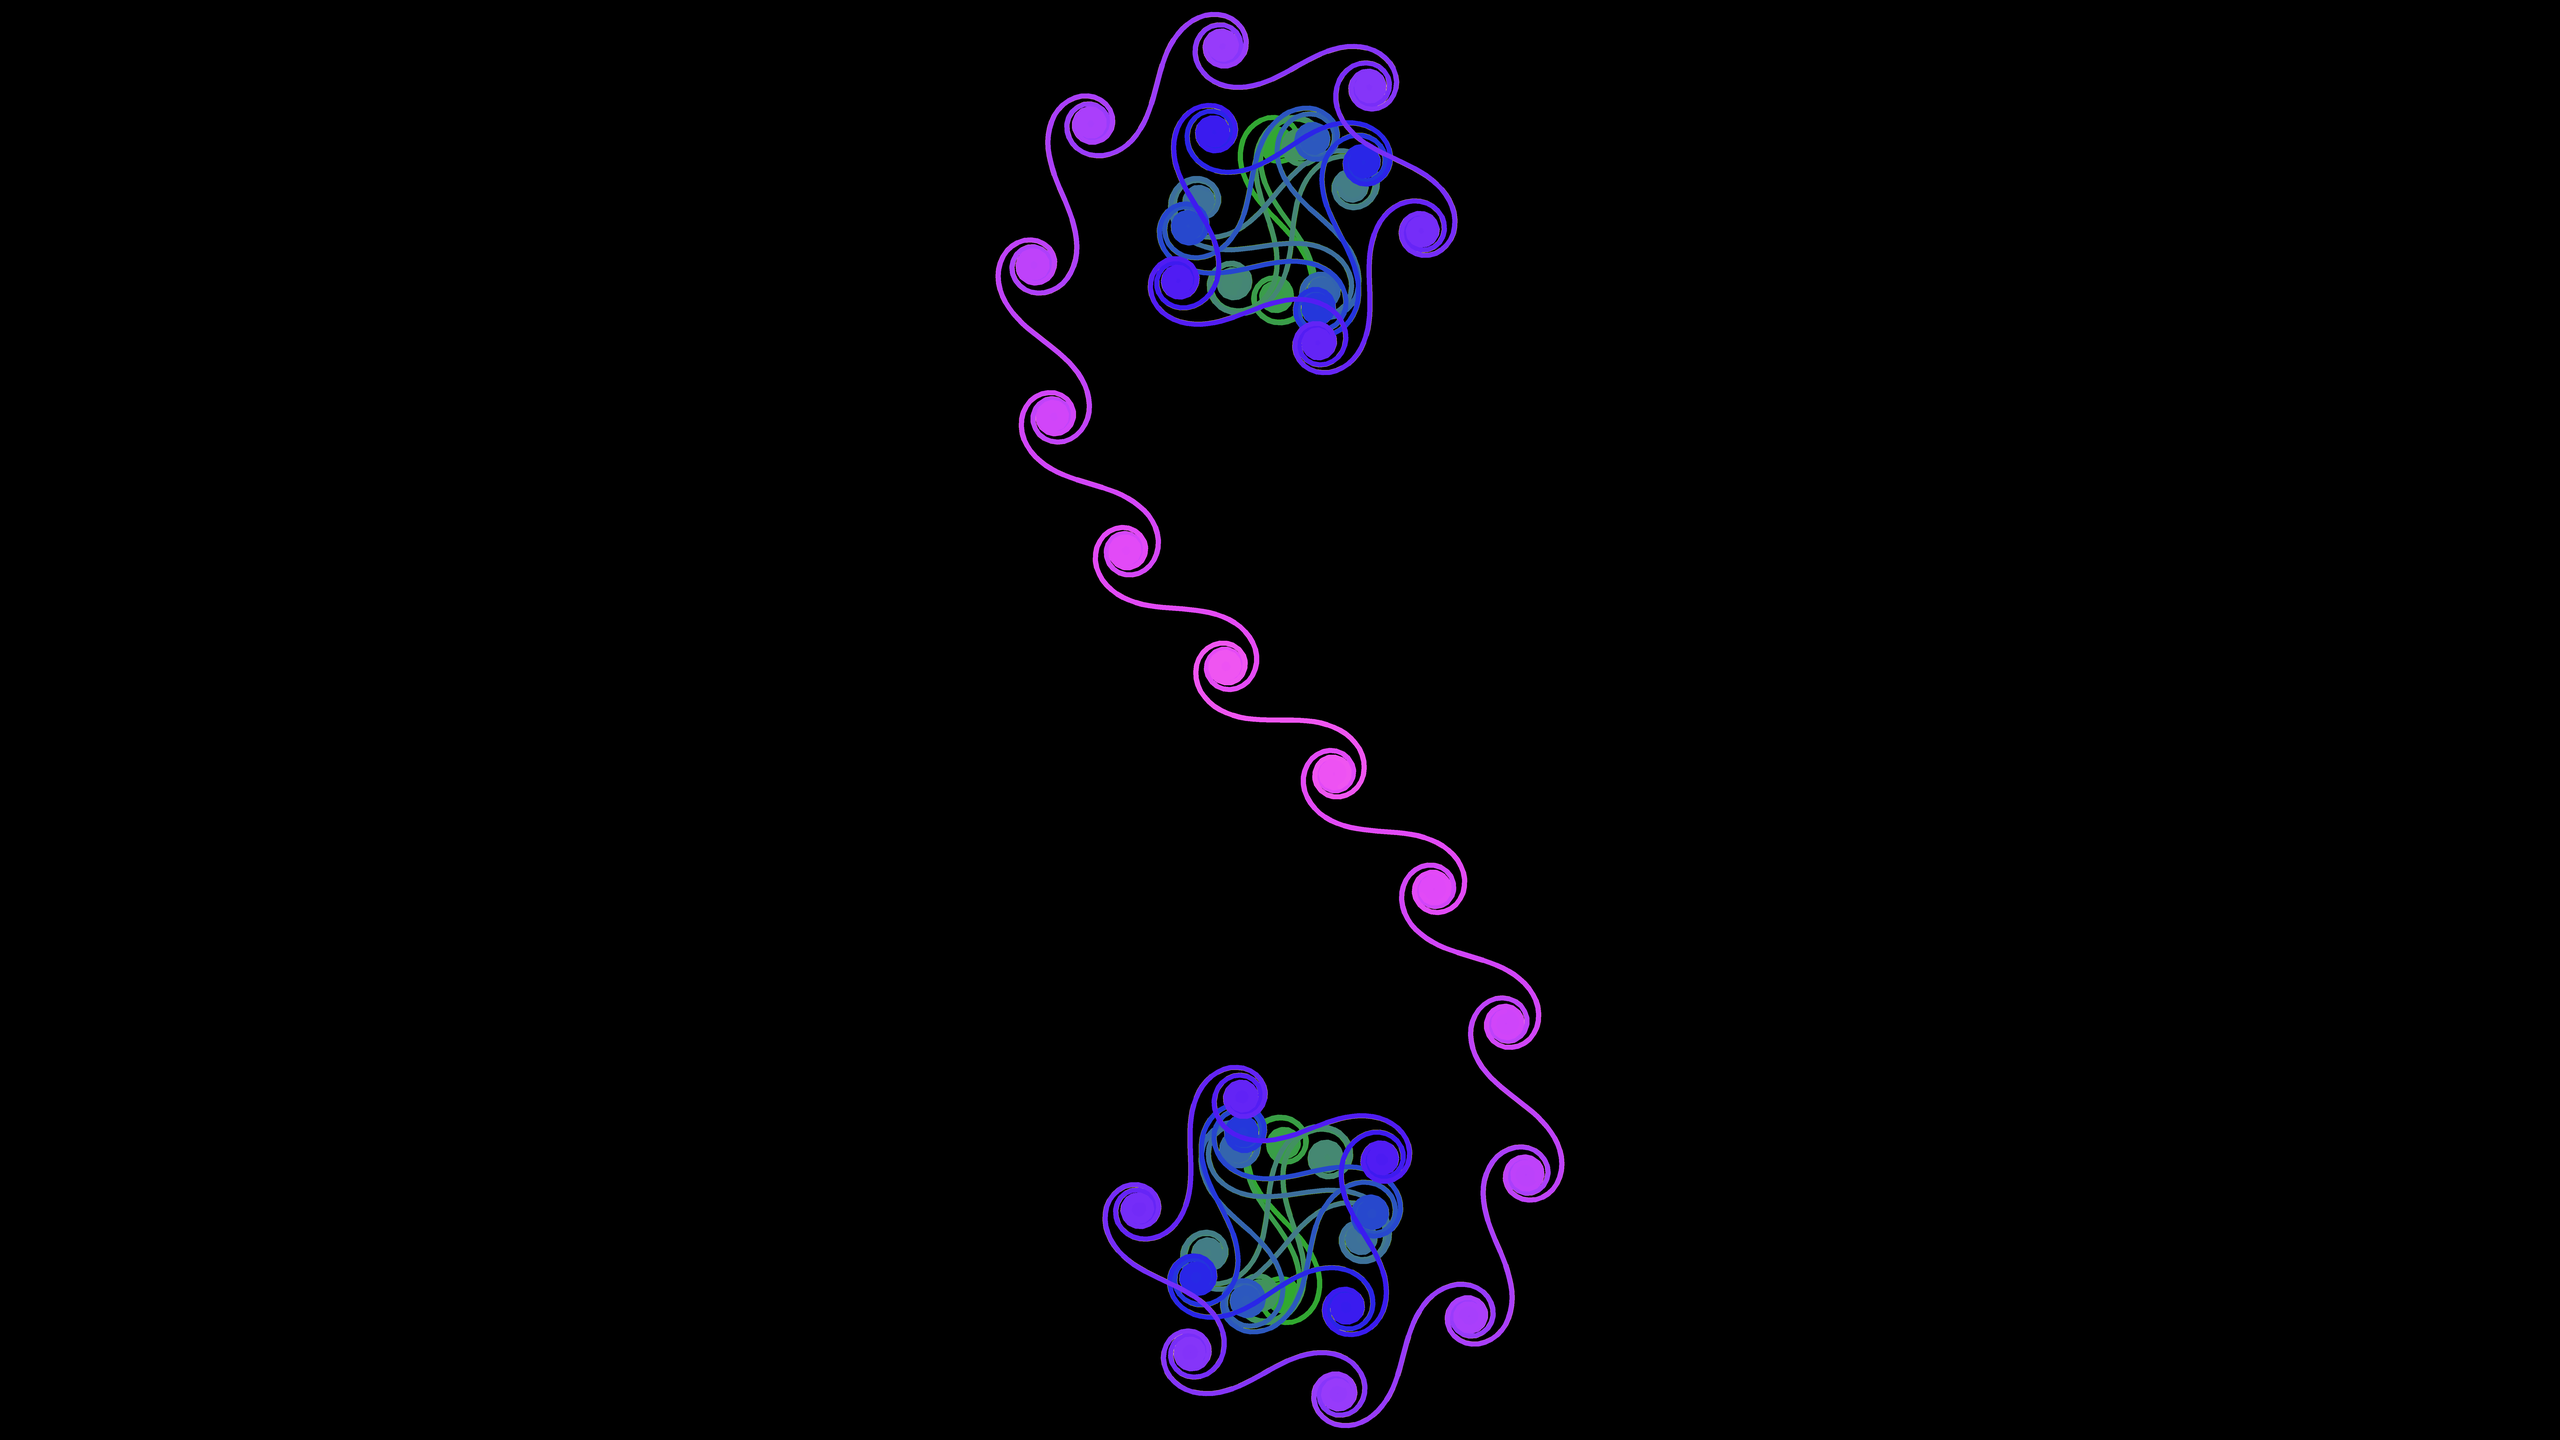
\includegraphics[width=0.3\textwidth]{./vertikal/tfa_046_p=043_q=21542_theta=0-71860_0_00_b_cyclic_mygbm_30_95_c78_Euler-Euler-Spiral_black.png}
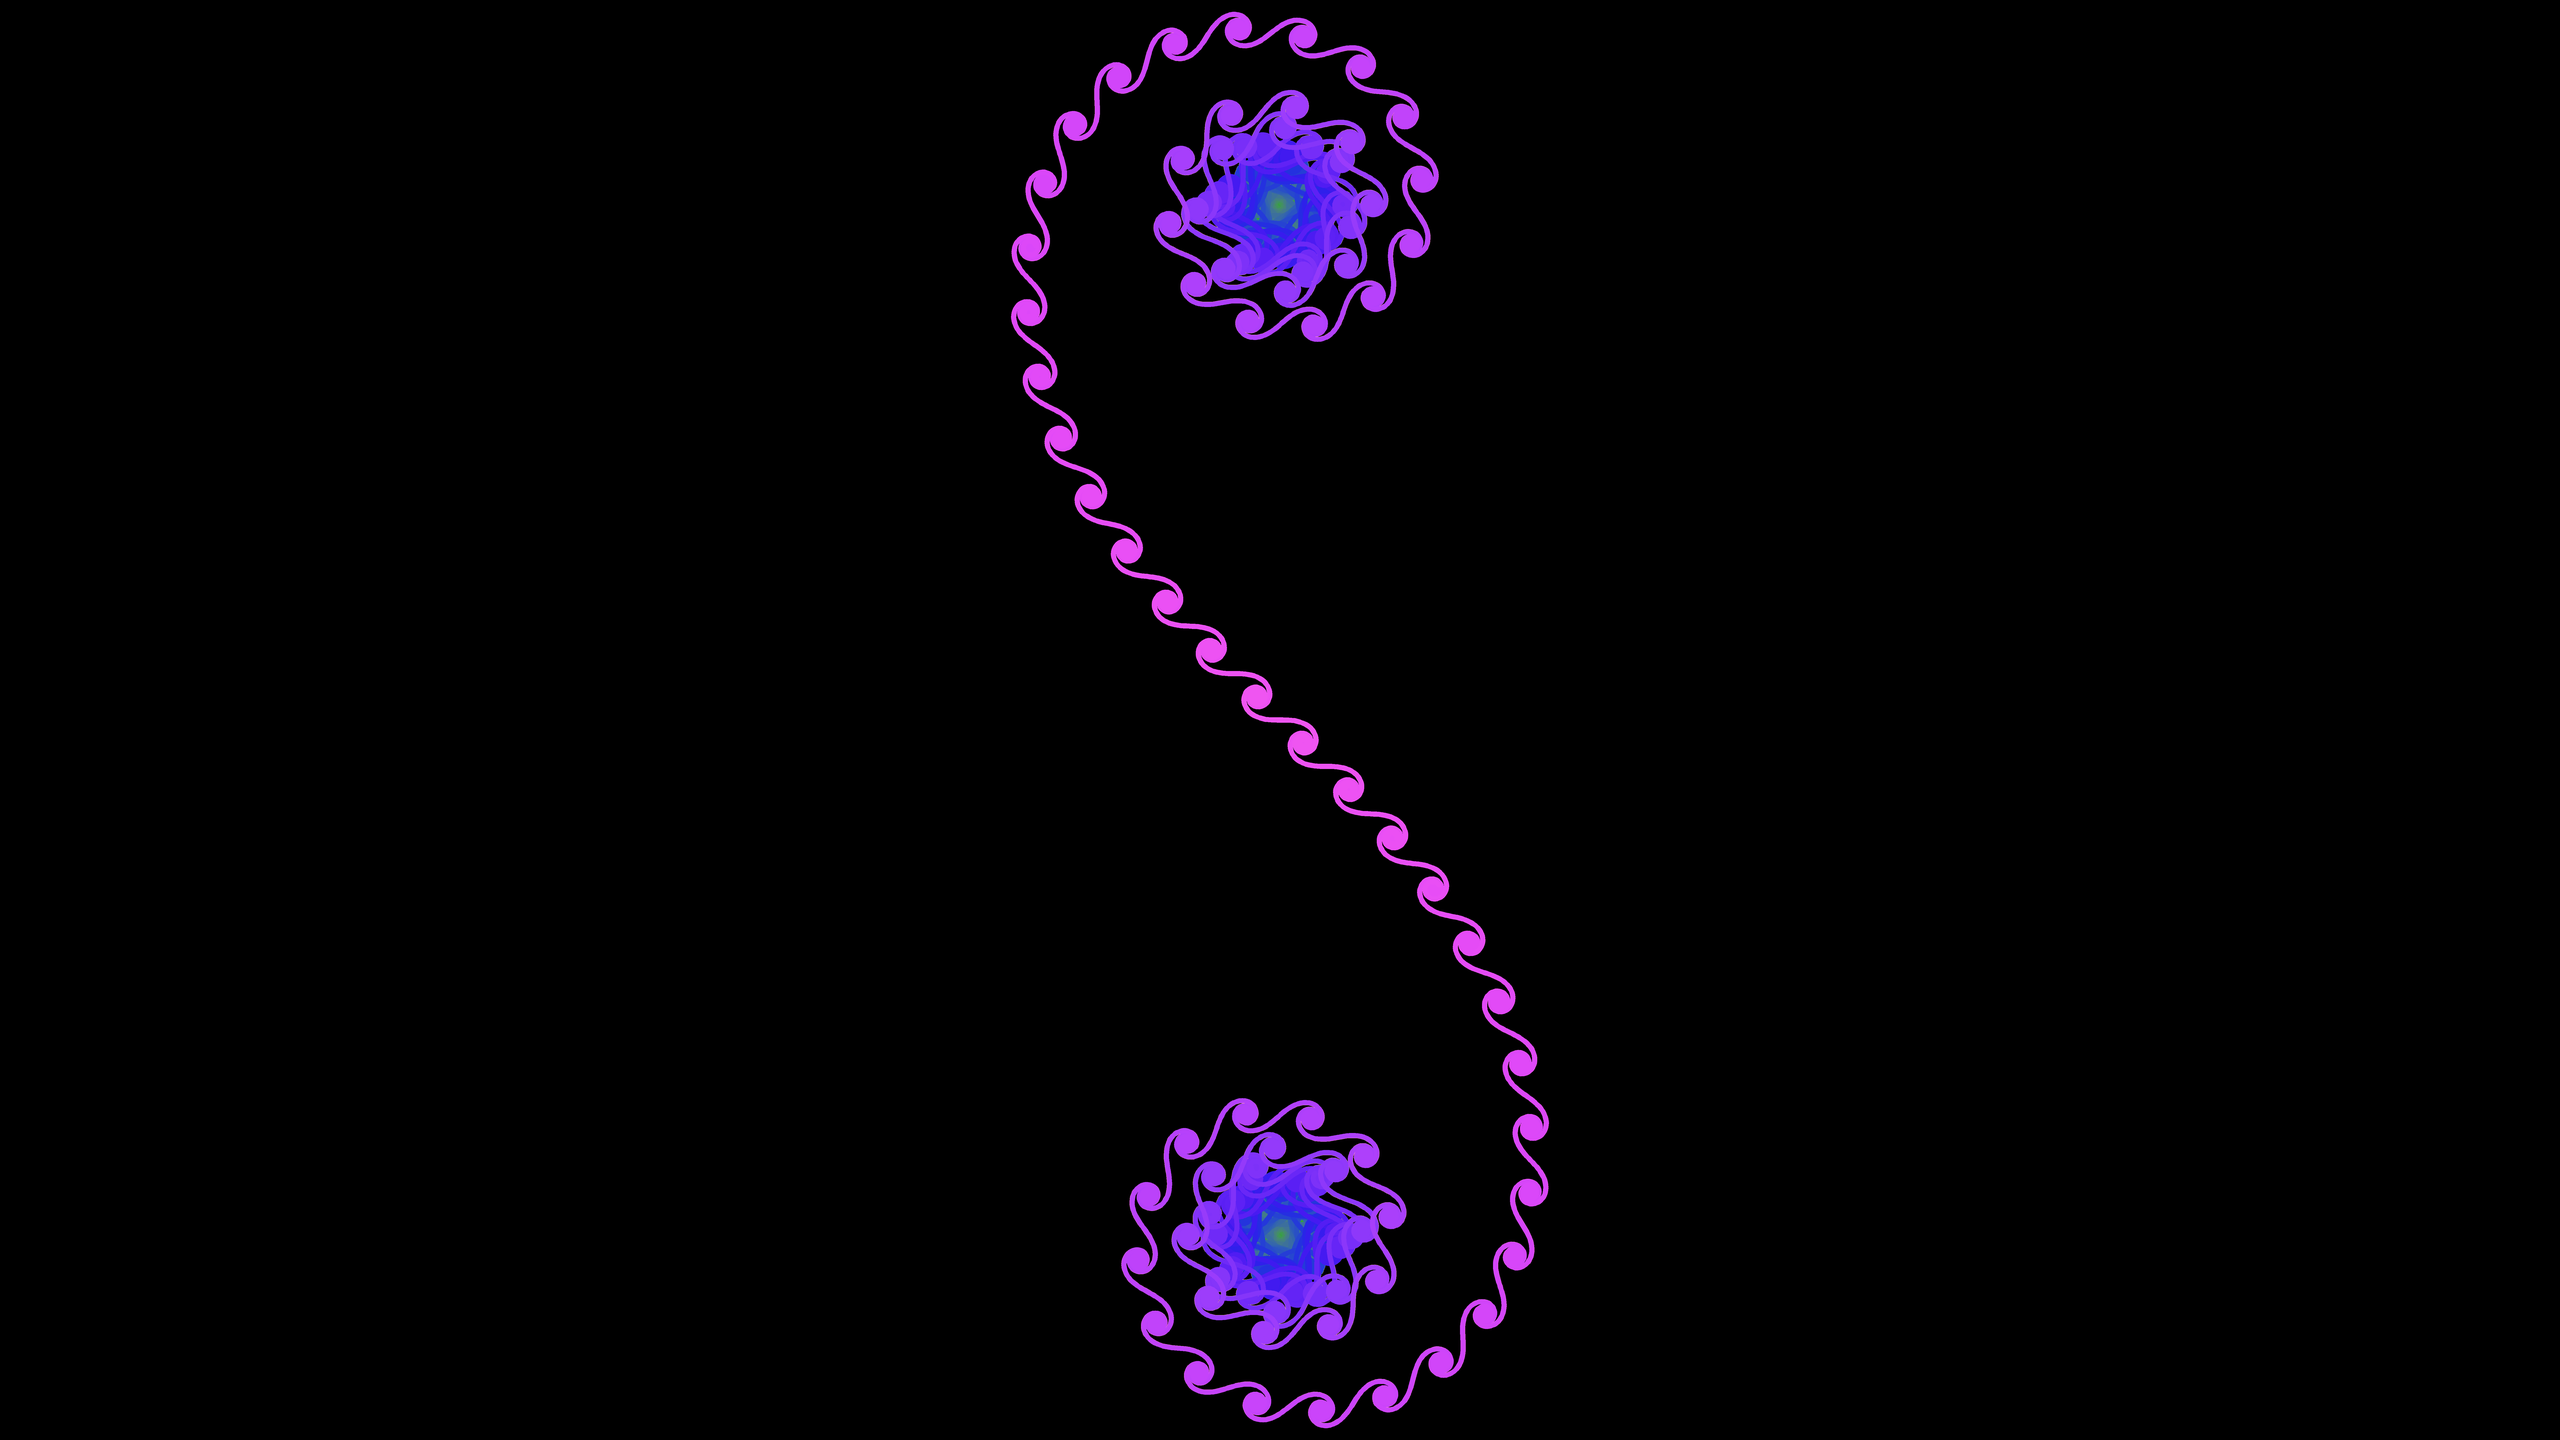
\includegraphics[width=0.3\textwidth]{./vertikal/tfa_046_p=249_q=124748_theta=0-71857_0_00_b_cyclic_mygbm_30_95_c78_Euler-Euler-Spiral_black.png}


\subsection{$q$ is odd}
In this case \(q+1\) is even so \(\total(q)=p\cdot\frac{q+1}{2}\) is a whole number.

Thus, when the sequence of angles is repeated, the turtle will have finished a whole number of rotations. If, and only
if, the turtle returned to its home at this point, will the set of visited points be finite.

Conjecture: These are the lines. It might be possible that the process ends up home in step \(q\), but that seems
unlikely and would produce an image that looks different than the usual images. I conjecture this does not actually
occur.

It would be interesting to see what happens around steps \(q/2-1/2\) and \(q/2+1/2\), because the lemma above still
holds. The turtle will draw the inverse of the path it did until here. There was just no 180° degree rotation like in
the case of \(q\) being even, so this does not lead back to the starting position.

\subsubsection{Experimental results}

The conjecture holds for the conducted experiments. Odd $q$ form lines. $p = 1$ forms the base element - a line build out
of Euler spirals. An increase in $q$ increases the number of lines
per Euler spiral which is conceived as an increase in resolution. The angle of the line compared to the origin moves
from horizontal to roughly 45° downwards in positive x direction with an increase in $q$.

Similar to even $q$, for a constant $p$, $p-1$ different lines are generated at maximum. Every increase of $q$ by $p$ produces the 
identical line form with a higher resolution as described above. As an odd $q$ has more freedom concerning the prime
factors, lines can be generated for even and odd $p$. Though infinite, there are more line turtles than returning turtles.

The lines take of at distinct angles. For an even $p$ the lines follow one of the four main axis directions (+x, -x, +y, -y),
assuming $q >> p$ and no change of angle due to low number of steps per base element (e.g. small $q$).
All four directions can be observed for a constant $p$ (e.g. $p = 60$).
For an odd $p$, the lines take of at a 45 Degree Angle from one of the four axis. For a constant $p$ only two directions are
filled with lines. For $p \in \{1, 5, 9, ..., 61, ...\}$ the lines go in the directions of +x-y or -x+y.
For $p \in \{3, 7, 11, ..., 59, ...\}$ the lines go in the direction of +x+y or -x-y.

For $p \in \{1, 5, 9, 25, 49\}$ all the lines run in the same direction (+x-y). With the exception of 1 and 5 these are all
squares of a prime. After experimental validation this seems to hold true as the result is as expected for $p \in \{121, 169, 289\}$.

This also holds true for $p \in \{81, 625\}$ - both primes to the power 4 - but not for $p = 27 = 3^3$.

\section{Taking the Position into Account}
Let us represent the position of the turtle in step \(\ell\) with \(p_\ell\in\mathbb{C}\) and its direction with
\(d_\ell\in\mathbb{C}\) with \(|d_\ell|=1\), i.e.\ \(d_\ell\) is a point on the unit circle. Then, at step \(\ell+1\), the turtle
will do:
\begin{align*}
p_{\ell+1} &= p_\ell + d_\ell &
c_{\ell+1} &= e^{(\ell+1)\cdot \theta\cdot 2\cdot \pi i} &
d_{\ell+1} &= d_ell\cdot c_{\ell+1} = d_\ell \cdot e^{\ell\cdot \theta\cdot 2\cdot \pi i}
\end{align*}
Defining \(p_0=0\) and \(d_0=1=e^0\), we can arrive at:
\[
d_\ell = e^{\theta\cdot 2\pi i\cdot \sum_{k=0}^\ell k}
= e^{\theta\cdot 2\pi i \cdot \ell\cdot(\ell+1)\frac{1}{2}}
= e^{\theta\cdot \pi i \cdot \ell\cdot(\ell+1)}
\]
This means for the position:
\[
p_\ell = \sum_{k=0}^\ell d_k
= \sum_{k=0}^\ell e^{\theta\cdot \pi i\cdot k\cdot(k+1)}
\]

Let's do some math and re-derive the Lemma above\footnote{Committing again an abuse of notation since \(c_\ell\) was
only meant to be defined for \(\ell\in\mathbb{N}\)}:
\begin{lemma}
\(c_{\frac{q}{2}-k} \cdot c_{\frac{q}{2}+k}=1\) for any \(k\in\mathbb{N}\). This means that the two rotations are
inverse to each other.
\end{lemma}
\begin{proof}
\begin{align*}
c_{\frac{q}{2}-k} \cdot c_{\frac{q}{2}+k}
&=e^{(\frac{q}{2}-k)\cdot \theta\cdot 2\cdot \pi i} \cdot e^{(\frac{q}{2}+k)\cdot \theta\cdot 2\cdot \pi i}
=e^{(\frac{q}{2}-k)\cdot \theta\cdot 2\cdot \pi i + (\frac{q}{2}+k)\cdot \theta\cdot 2\cdot \pi i}
=e^{q\cdot \theta\cdot 2\cdot \pi i} \\
&=e^{q\cdot \frac{p}{q}\cdot 2\cdot \pi i} 
=e^{p\cdot 2\cdot \pi i} 
=1^p
=1
\end{align*}
\end{proof}
Now we can show that the turtle returns to its starting orientation for odd \(q\). For even \(q\), it will face in the opposite direction.
\begin{lemma}
In general, \(d_q=(-1)^p\).
For even \(q\), this means that \(d_q=-1\).
\end{lemma}
\begin{proof}
Let us start with \(d_q\) as the product of the individual changes in directions. This product is then re-arranged into
certain combinations.
\begin{align*}
d_q
&= \prod_{\ell=0}^q c_\ell
= c_{\frac{q}{2}} \cdot \prod_{\ell=1}^{\frac{q}{2}-1} c_{\frac{q}{2}+\ell} \cdot c_{\frac{q}{2}-\ell}
\intertext{At this point the lemma can be applied and it only remains to compute \(c_{\frac{q}{2}}\):}
&= c_{\frac{q}{2}} \cdot \prod_{\ell=1}^{\frac{q}{2}-1} 1
= c_{\frac{q}{2}}
= e^{\frac{q}{2}\cdot \theta\cdot 2\cdot \pi i}
= e^{\frac{q}{2}\cdot \frac{p}{q}\cdot 2\cdot \pi i}
= e^{p\cdot \pi i}
= \left(e^{\pi i}\right)^p
= (-1)^p
\end{align*}
Since we assume that \(p\) and \(q\) are coprime, if \(q\) is even, then \(p\) must be odd. In this case, we arrive at
\(d_q=-1\). If \(q\) is odd, then \(p\) can be odd or even and we cannot conclude anything.
\end{proof}
I have no good ideas on how to continue here.

One good idea: Test whether these results actually hold. I have only derived them, but never tested them.

\section{The Continuous Case}
Instead of having two discrete steps (move forward one step, rotate, repeat), one could also consider a continuous
setting: While moving forwards, the turtle rotates at the same time. In the discrete times, the rotation increases
linearly with the number of steps. The continuous equivalent would be \(\rotate(t)=t\cdot\theta\), which leads to a
direction at time \(t\) of \(\total(t)=\int_{x=0}^t\rotate(t)\,\text{d}x=t^2\theta/2\).

More interesting is the position which is a complex number starting at \(p(0)=0\) and evolving via:
\[
\dot{p}(t) = e^{2\pi i \cdot \total(t)} = e^{\pi i \cdot t^2\theta}
\]
The author of these lines asked
\href{https://www.wolframalpha.com/input?i=p%28t%29+%3D+integrate+e%5E%28pi+*+i+*+x%5E2+*+phi%29+from+x%3D0+to+t}{Worlfram Alpha}
and got the following solution, where erf is the so-called error function\footnote{Which the author never
encountered before}:
\[
p(t) = -\frac{\sqrt[4]{-1}\;\text{erf}((-1)^{\frac{3}{4}}\sqrt{\pi}t\sqrt{\phi})}{2\sqrt{\phi}}
\]
This can now be
\href{https://www.wolframalpha.com/input?i=parametric+plot%5BReal%28-%28%28-1%29%5E%281%2F4%29+erf%28%28-1%29%5E%283%2F4%29+sqrt%28pi%29+t+sqrt%28pi%2F2%29%29%29%2F%282+sqrt%28pi%2F2%29%29%29%2C+Imag%28-%28%28-1%29%5E%281%2F4%29+erf%28%28-1%29%5E%283%2F4%29+sqrt%28pi%29+t+sqrt%28pi%2F2%29%29%29%2F%282+sqrt%28pi%2F2%29%29%29%5D+for+t%3D0..20}{plotted},
for example with \(\phi=90^\circ=\pi/2\) and \(t\) from 0 to 1, and then from 0 to 20:

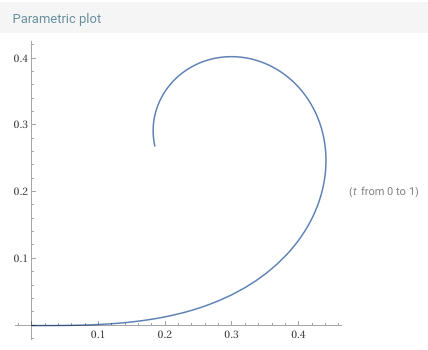
\includegraphics[width=\textwidth]{continuous1.png}

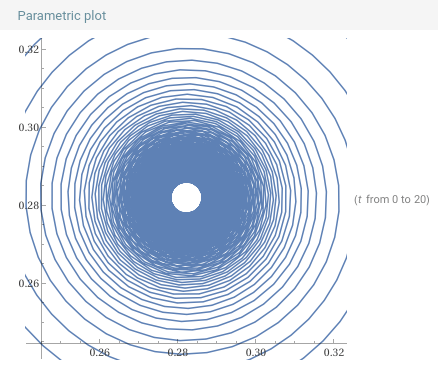
\includegraphics[width=\textwidth]{continuous20.png}

\section{Interaction between uneven and even q}

When we take $\theta = \frac{3}{3 \cdot 500 + 1} \cdot 360^{\circ}$ it forms a line as expected.

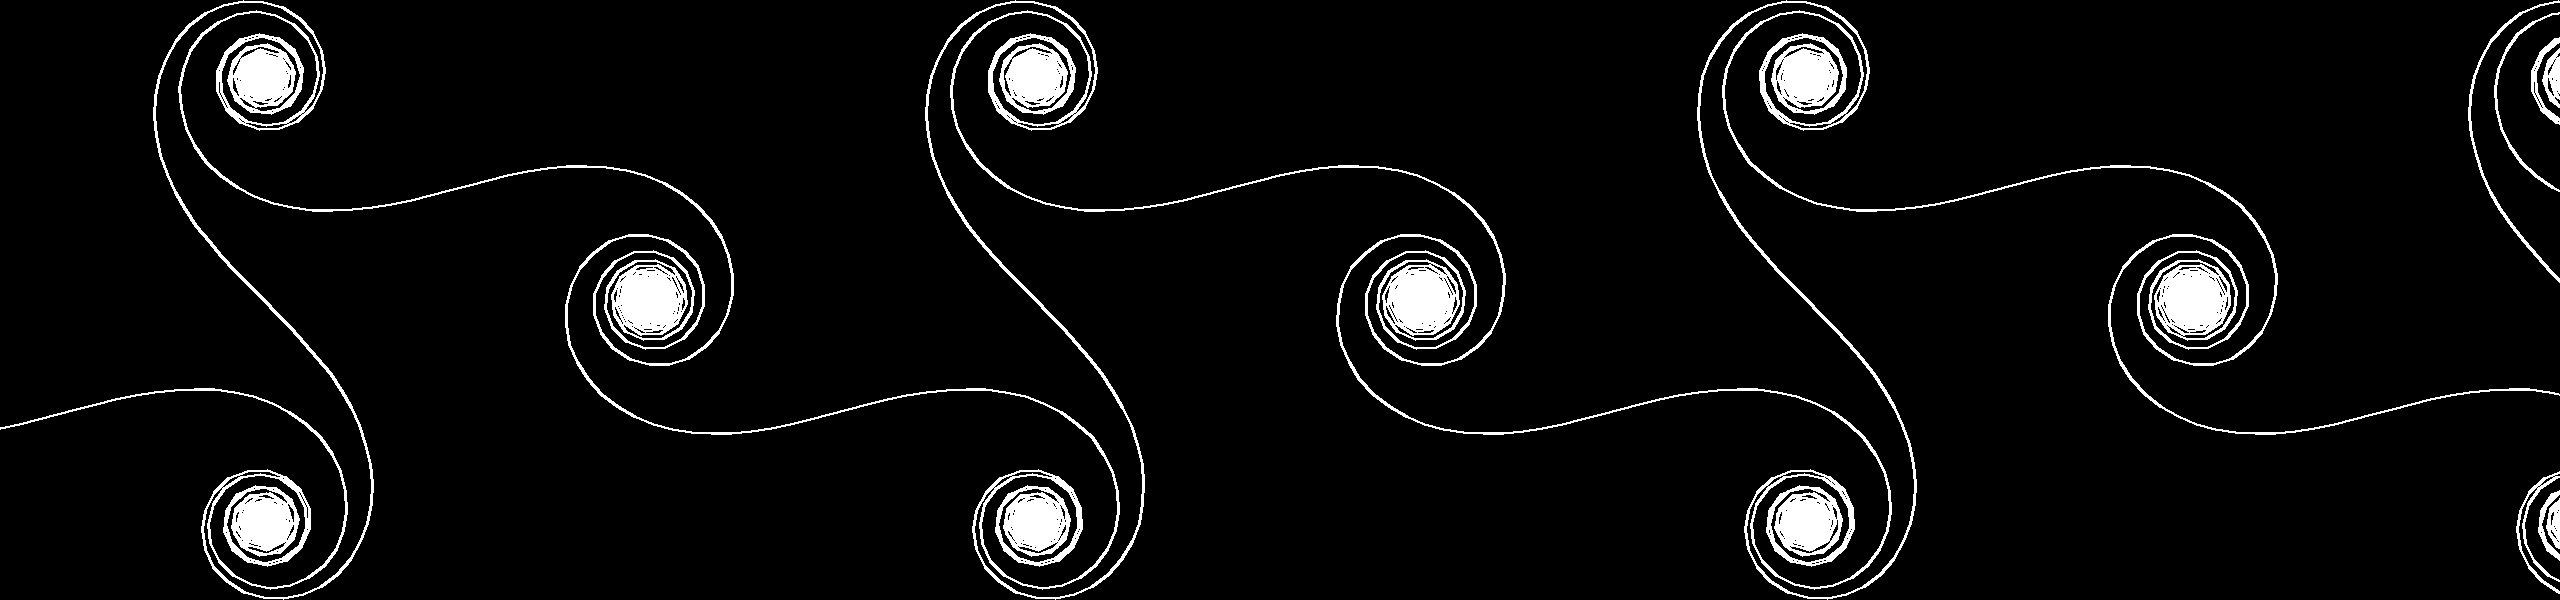
\includegraphics[width=\textwidth]{tfa_049_p=003_q=001501_000-71952032_linesample.png}

How can we purposfully create further images using this line as a basis? For example $\theta = \frac{625}{625*501 + 208} \cdot 360^{\circ}$
to form another line based on the first line.

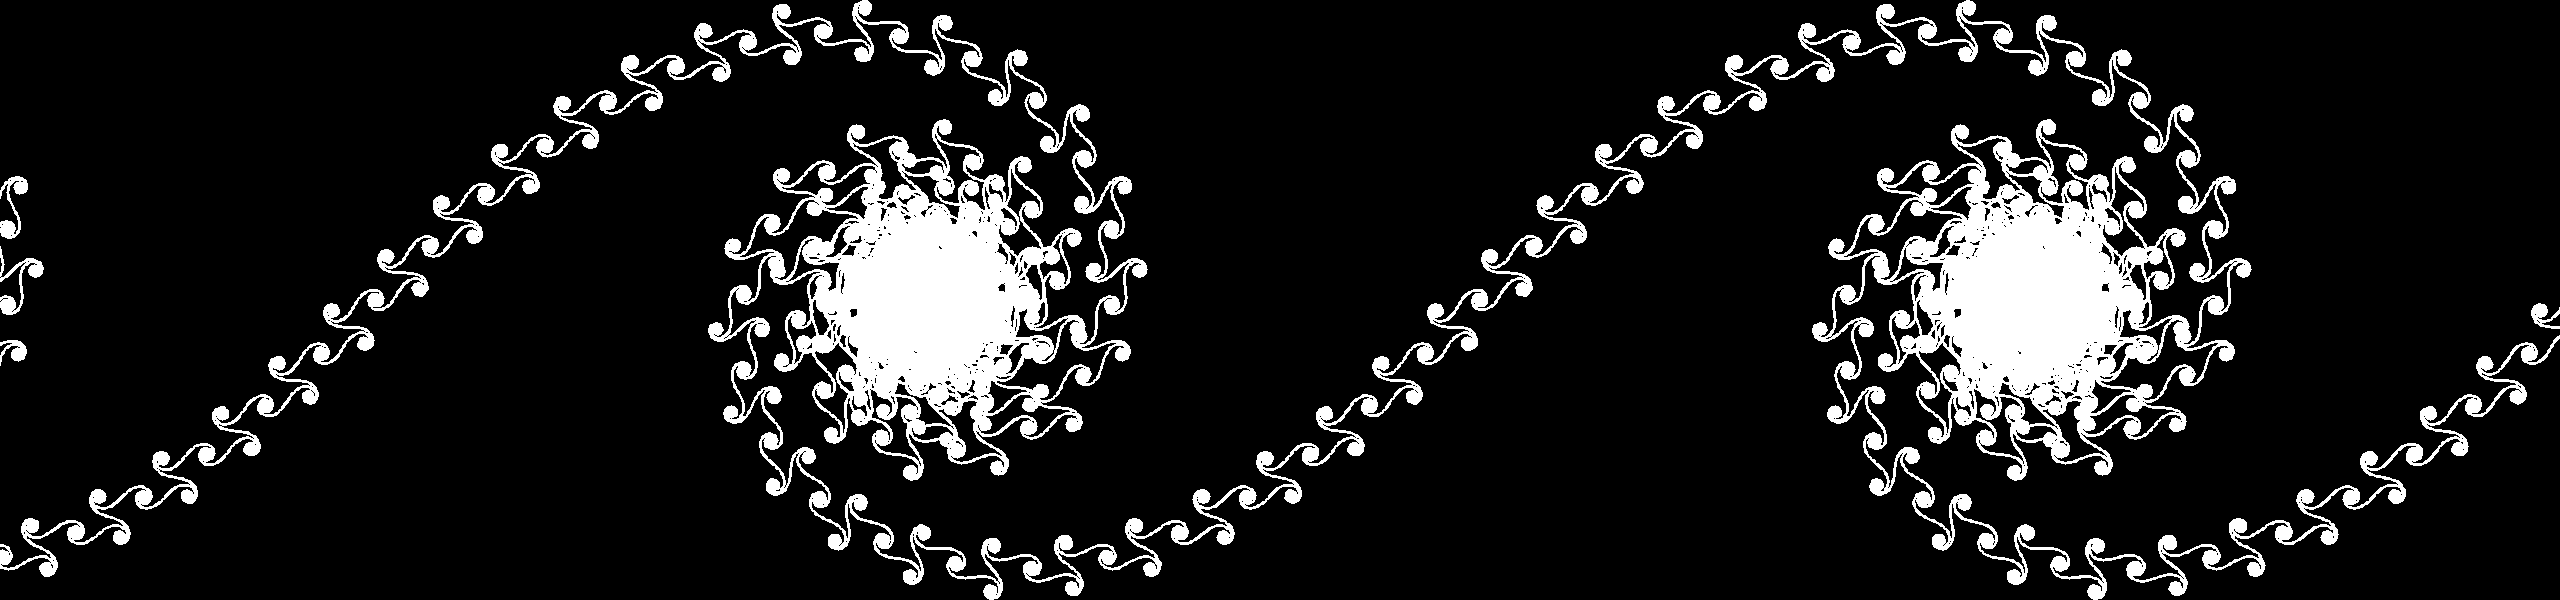
\includegraphics[width=\textwidth]{tfa_049_p=625_q=313333_000-71808587_linesample.png}

Or returning images like $\theta = \frac{661}{661 \cdot 500 + 220} \cdot 360^{\circ}$

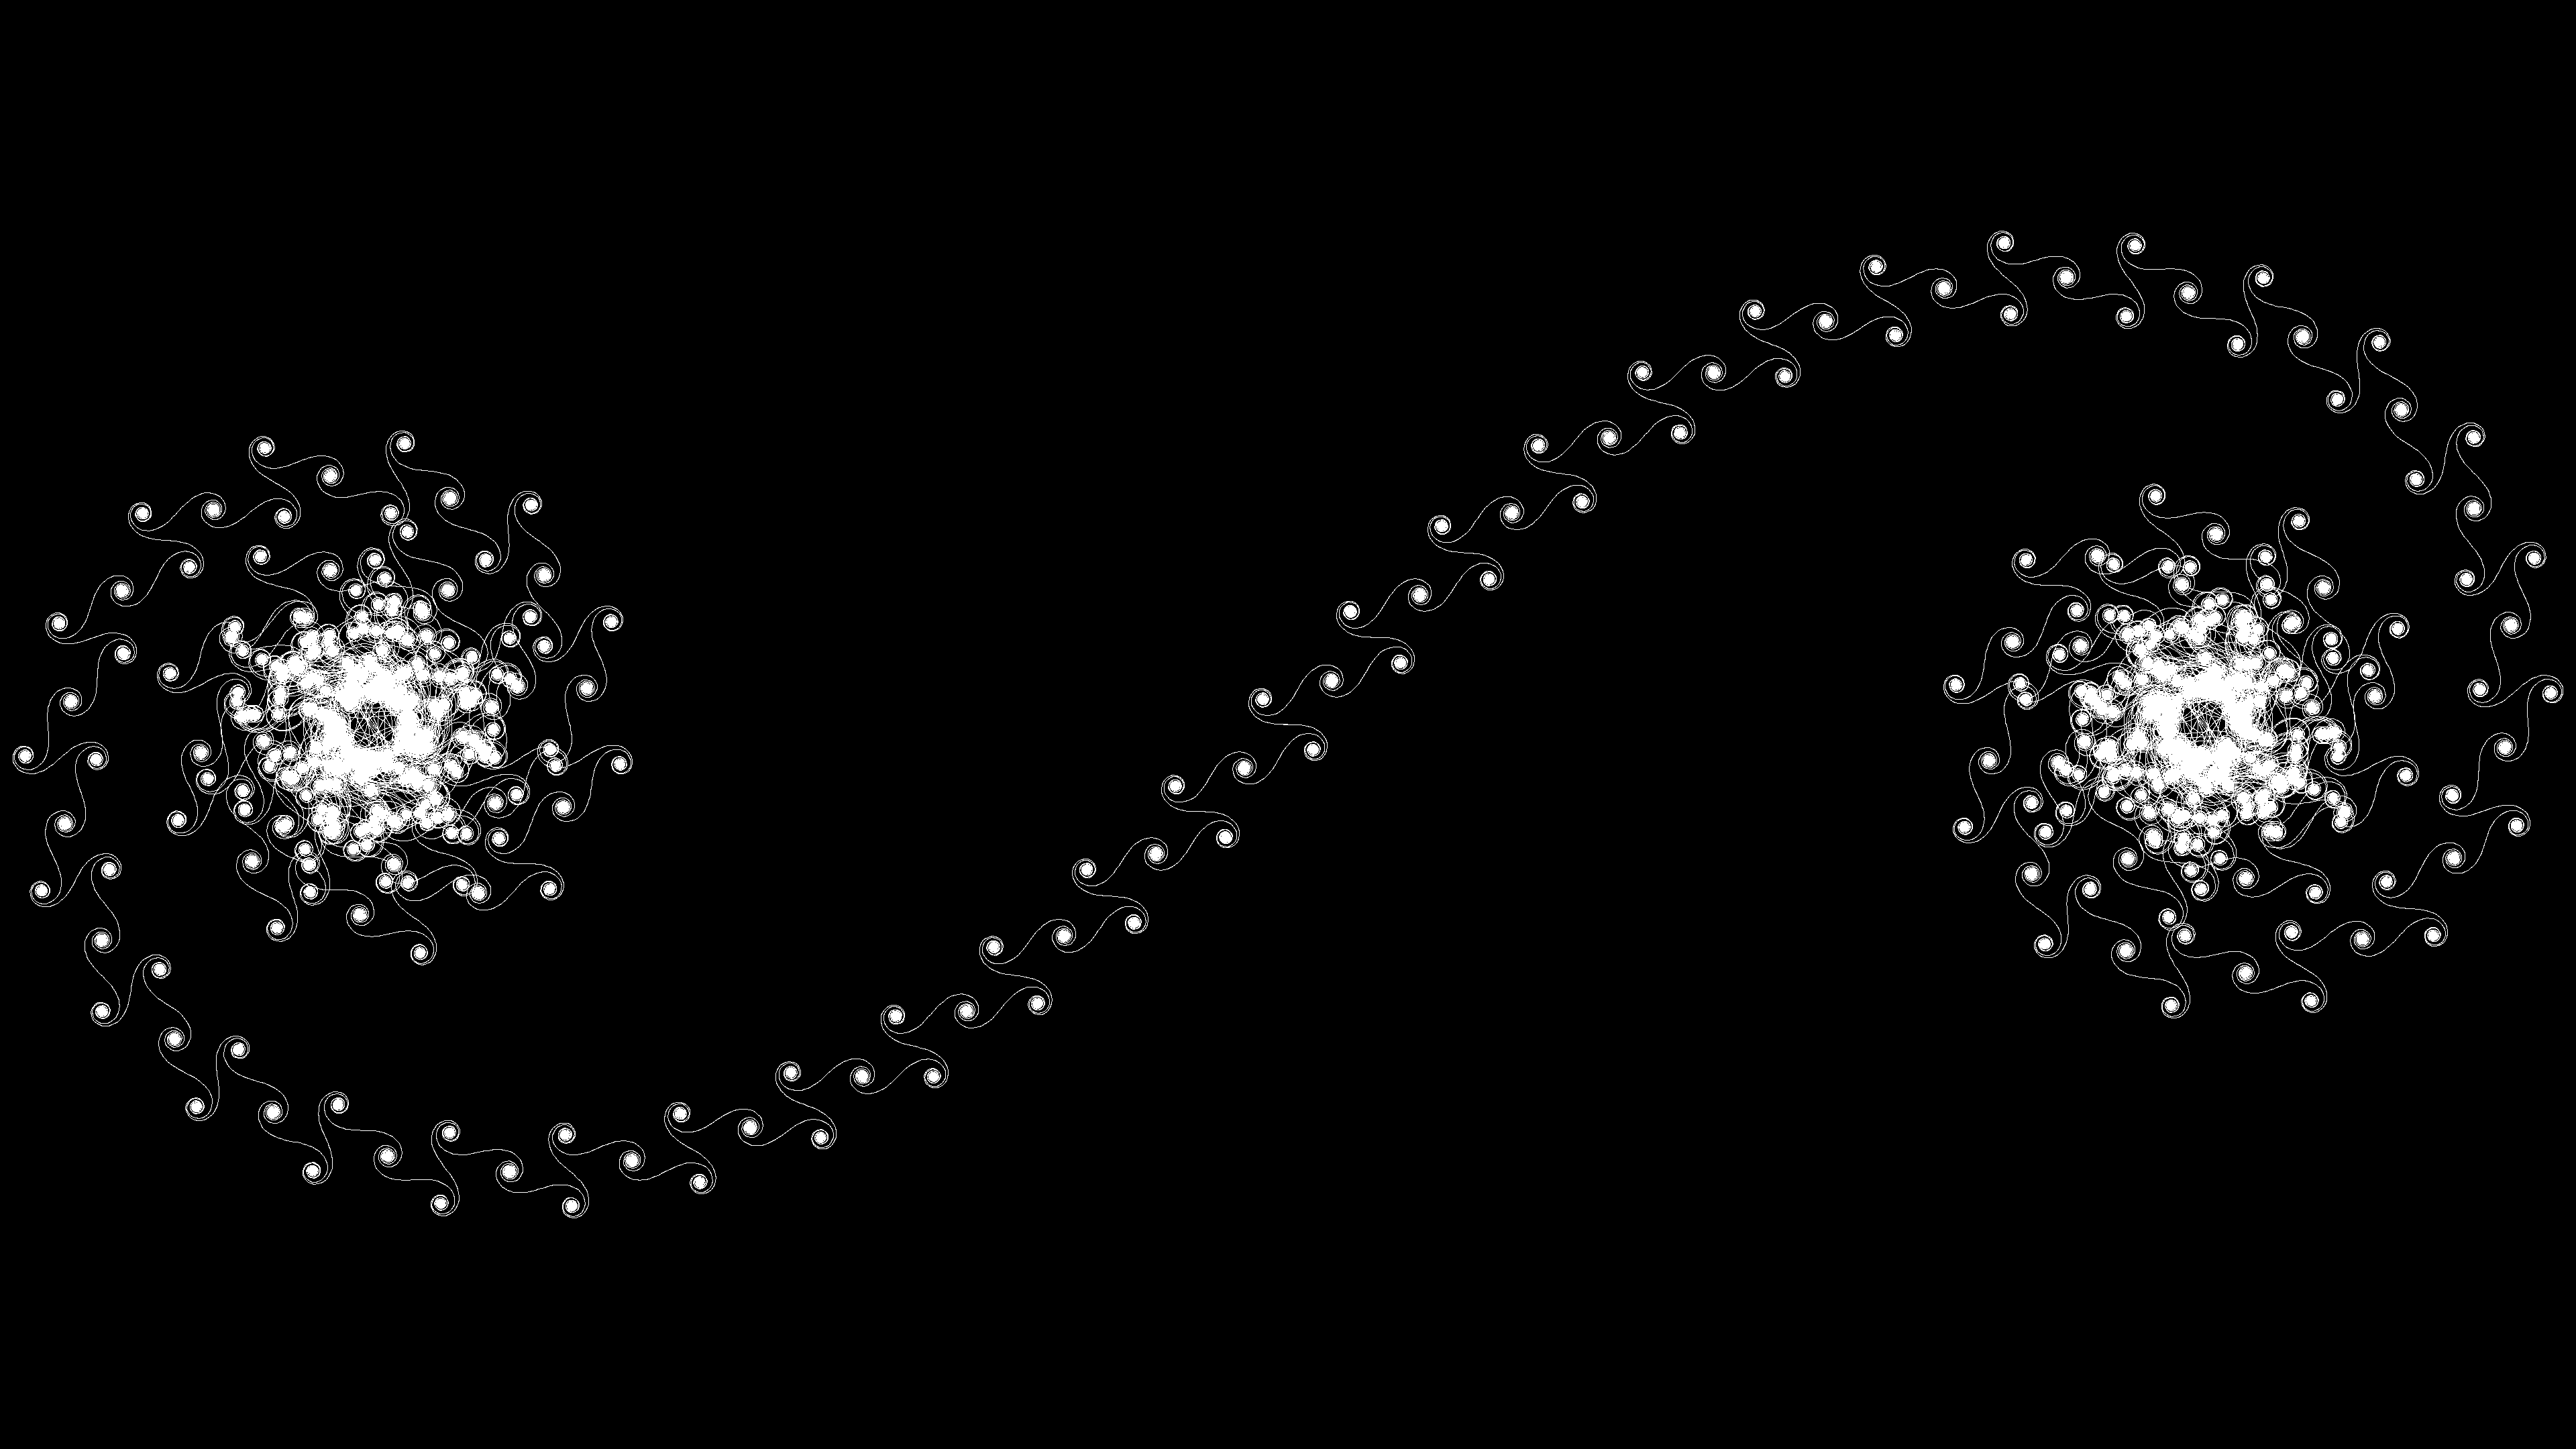
\includegraphics[width=\textwidth]{tf_p=661--q=330720--theta=000_71952104.png}

So how about the same $p$ - so looking at $\theta = \frac{625}{625 \cdot 500 + 208} \cdot 360^{\circ}$ we find:

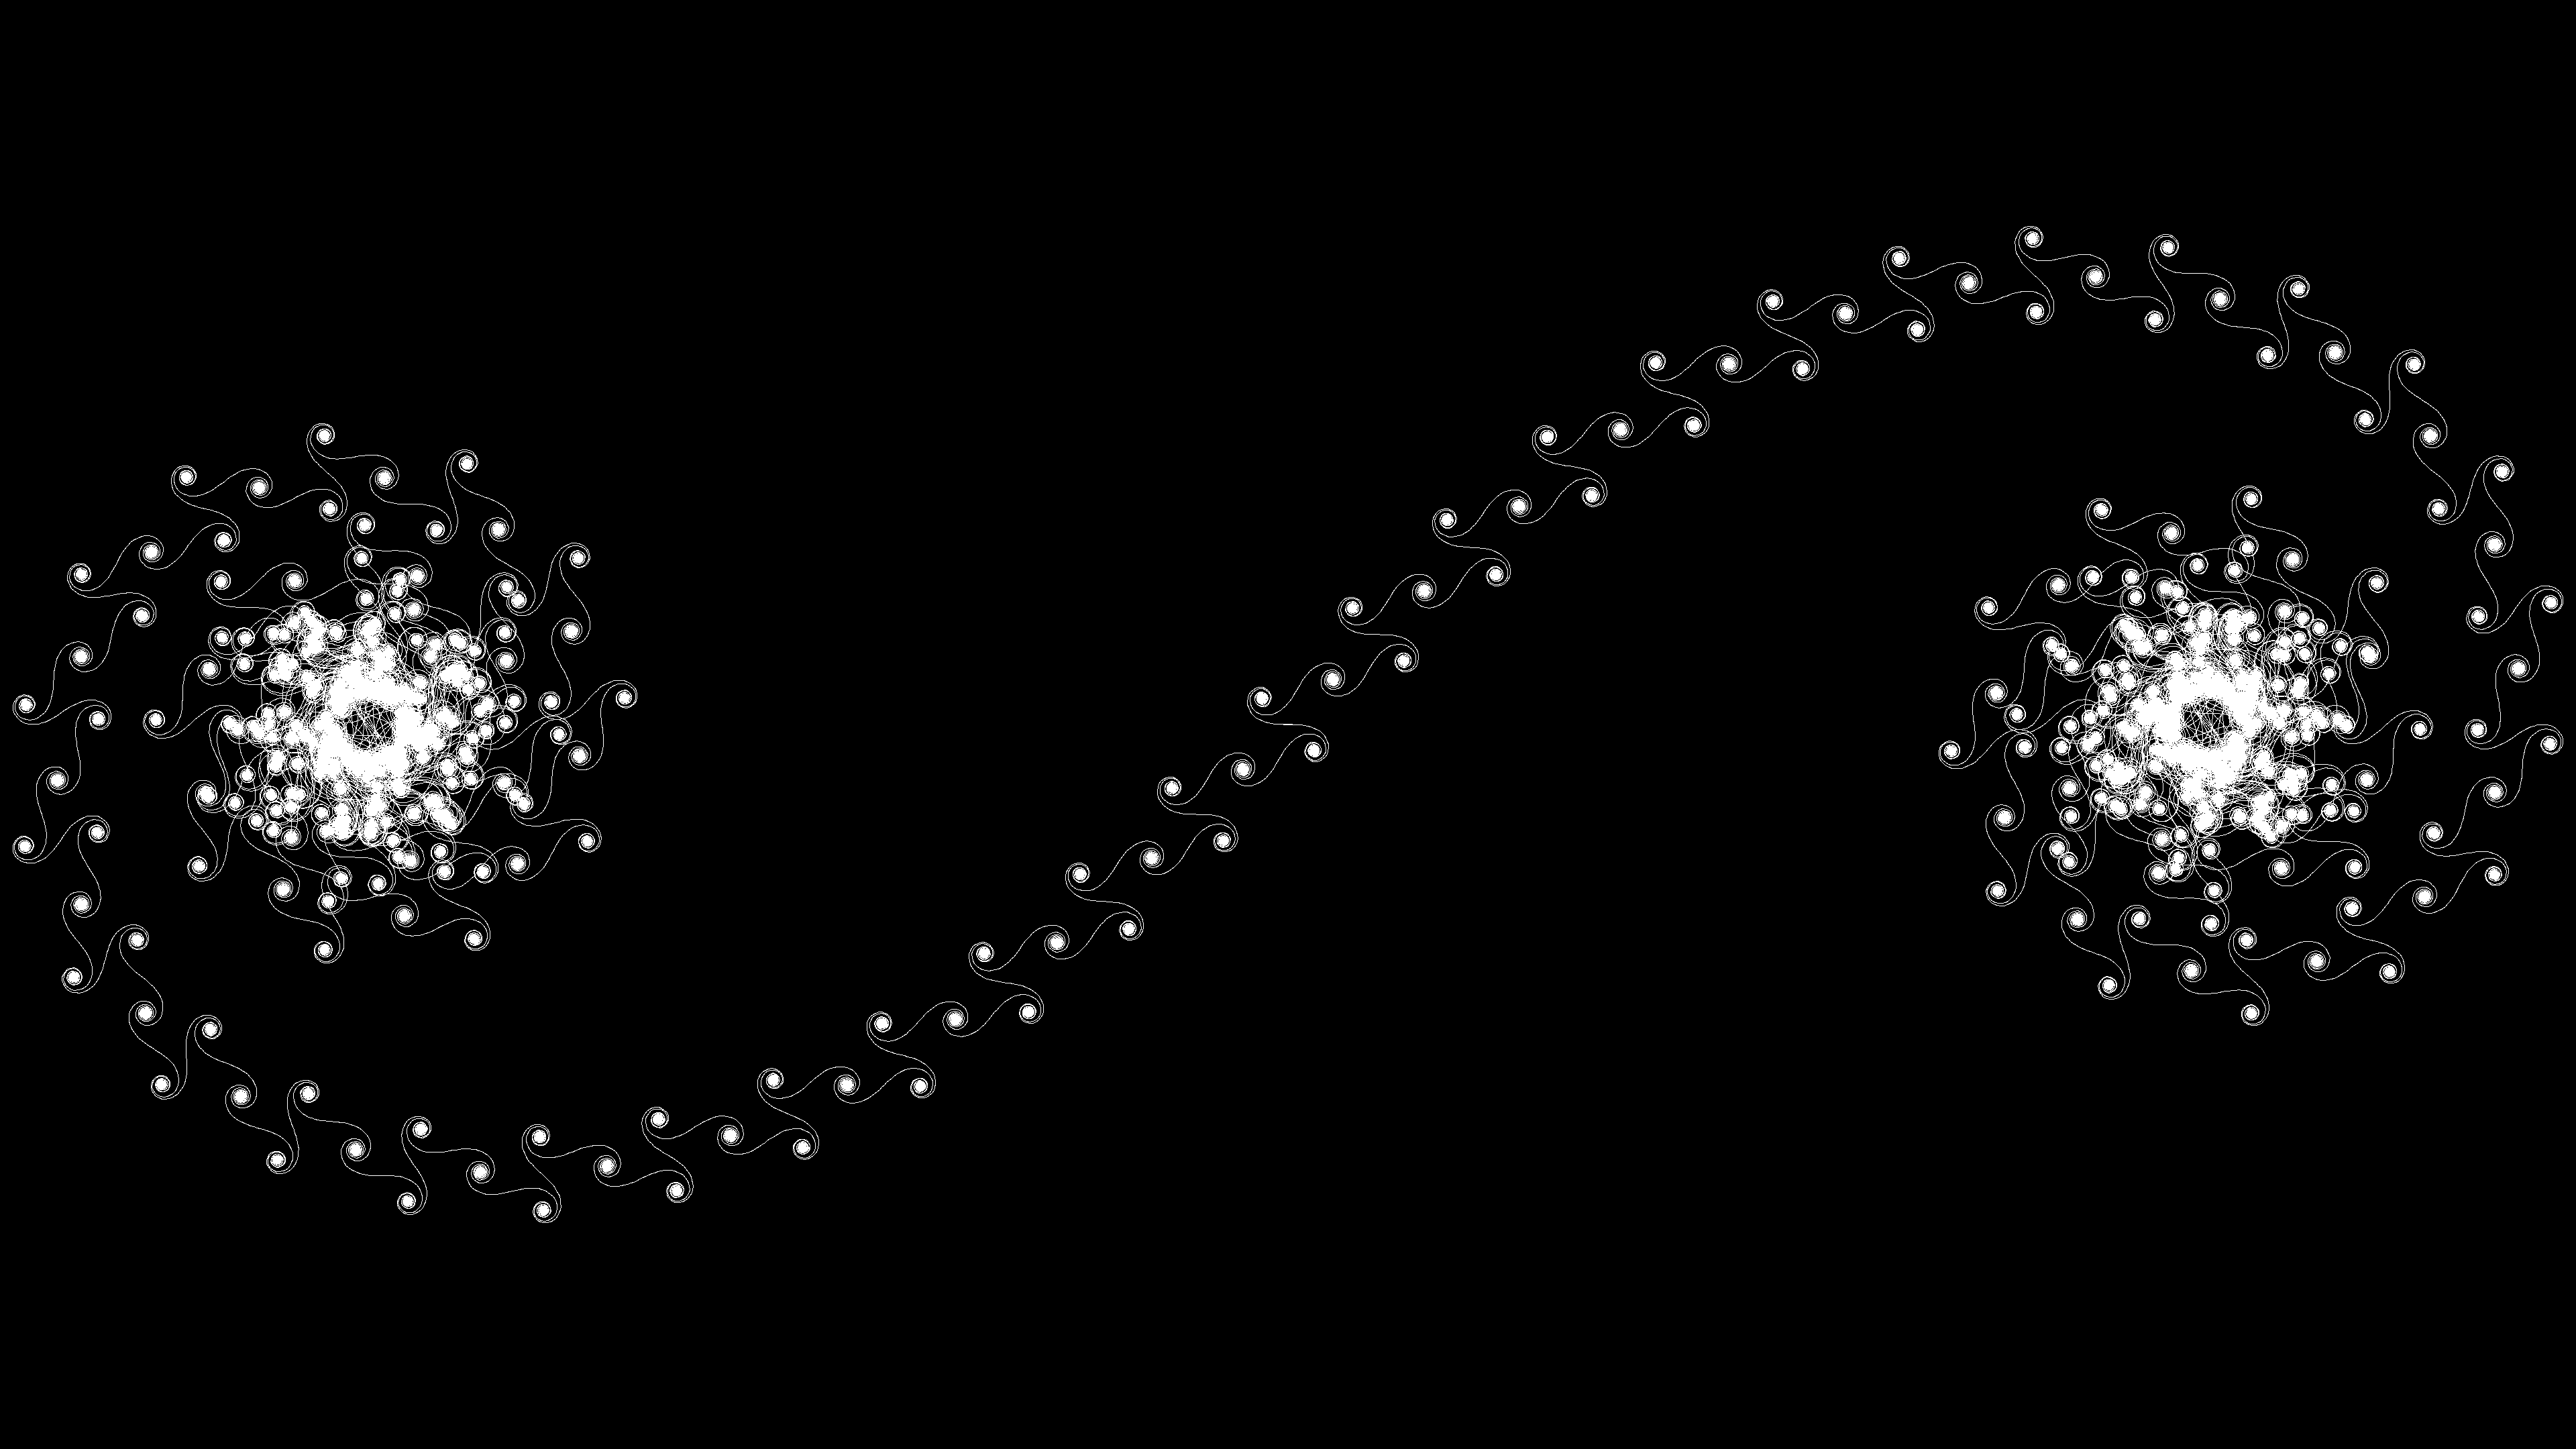
\includegraphics[width=\textwidth]{tf_p=625--q=312708--theta=000_71952109.png}

So the idea would be to define $\theta$ new in the form of $\theta = \frac{p}{p \cdot s + n} \cdot 360^{\circ}$. With $p=const, n=const$ and $n \in \{0, ..., 2\cdot (p-1)\}$
the difference between the returning version and the line version is increasing s by 1. See chapter \ref{app:A} for a sample Study with $p = 499$
(as 499 is prime an therefor easy on $q$).

Examples where the connection can be spotted easily are Figures \ref{fig:n=050}, \ref{fig:n=100}, \ref{fig:n=166}, \ref{fig:n=250}, \ref{fig:n=312}.

At this point one might propose latest to rewrite $\frac{p}{q}$ as $\frac{p}{p \cdot s + n}$ with $p$ being the number of Euler spirals in one iteration,
$s$ being the number of steps per Euler spiral and $n$ being the image selector or szenario selector within one image series defined by $p$.



% \section{Acknowledgements}
% Thanks a lot to Schneirob for producing \url{https://www.youtube.com/watch?v=Fx1d8x0gIu4}. This made it really easy for
% me to get an overview over things and identify some interesting angels. Then I used
% \url{https://github.com/schneirob/turtlefun} to get the angles that occur during the Euler spiral. All the hard parts
% were already prepared for me.

\section{Appendix A}\label{app:A}
\begin{figure}[H]
  \centering
  \begin{subfigure}[t]{0.48\textwidth}
    \centering
    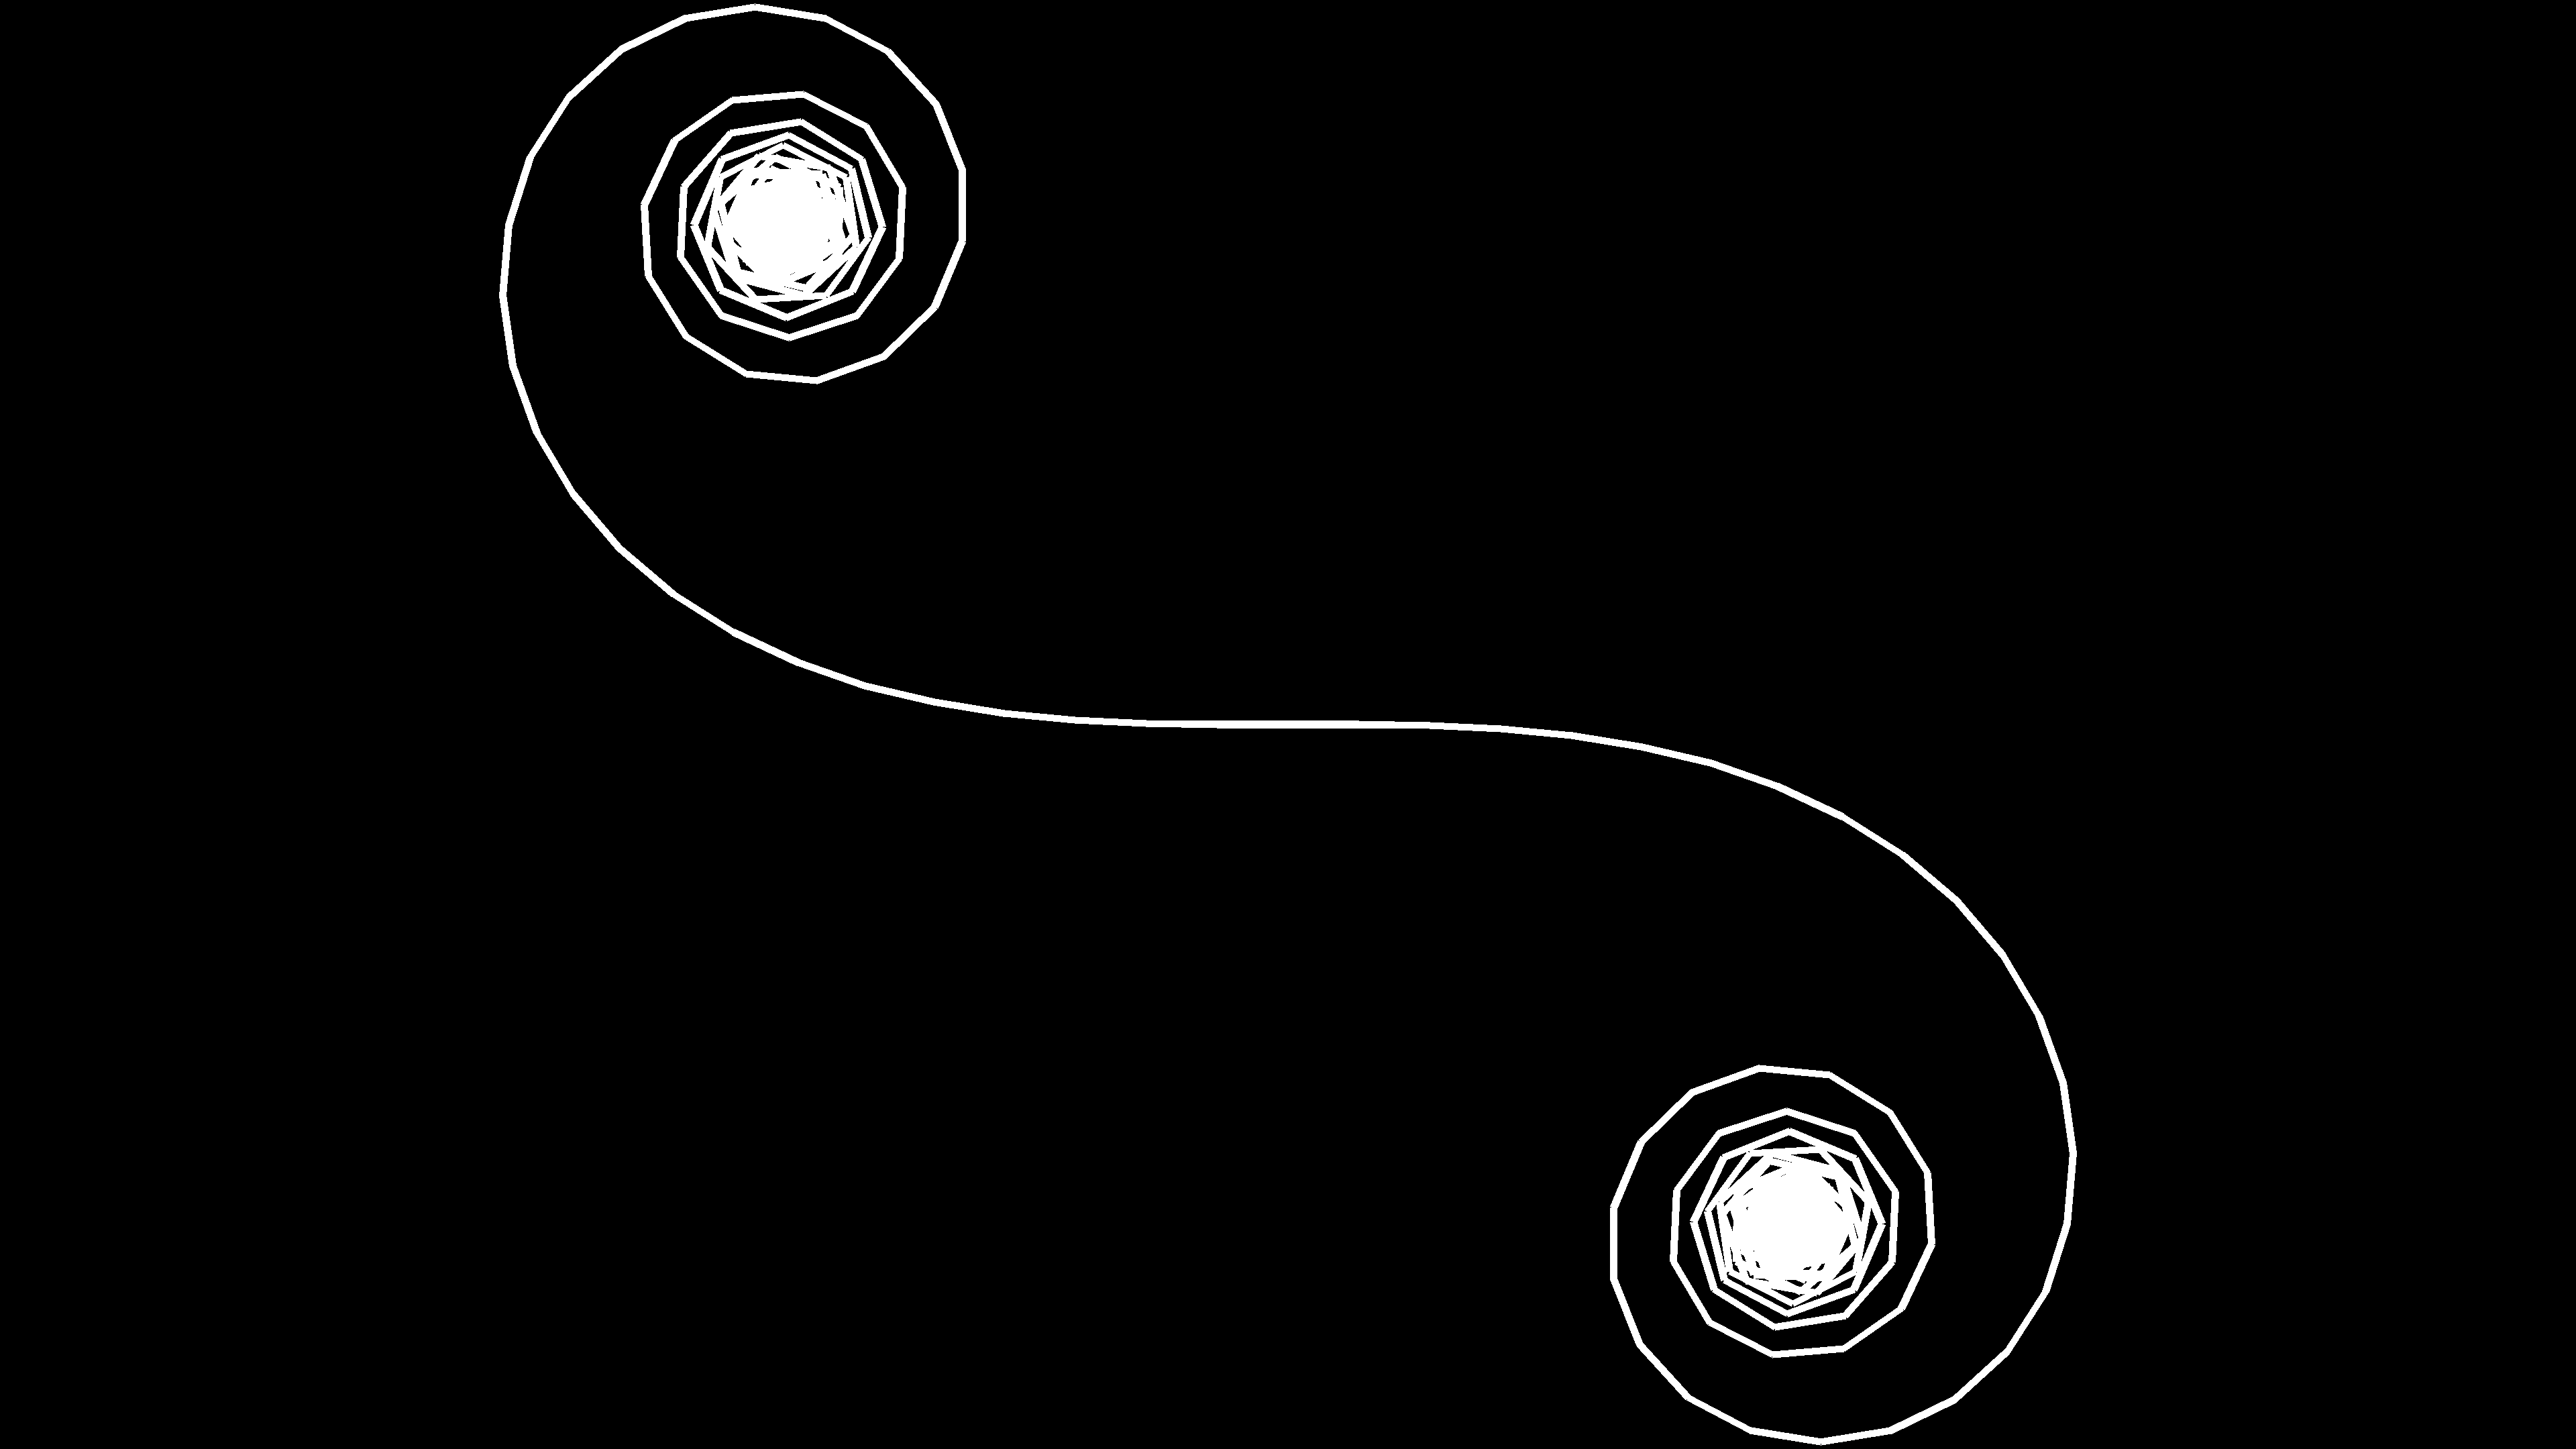
\includegraphics[width=\linewidth]{./stepsplusoneimages/0000000001.png}
    \caption{tf p=499 q=199600 theta=000 90000000.png}
  \end{subfigure}
  \begin{subfigure}[t]{0.48\textwidth}
    \centering
    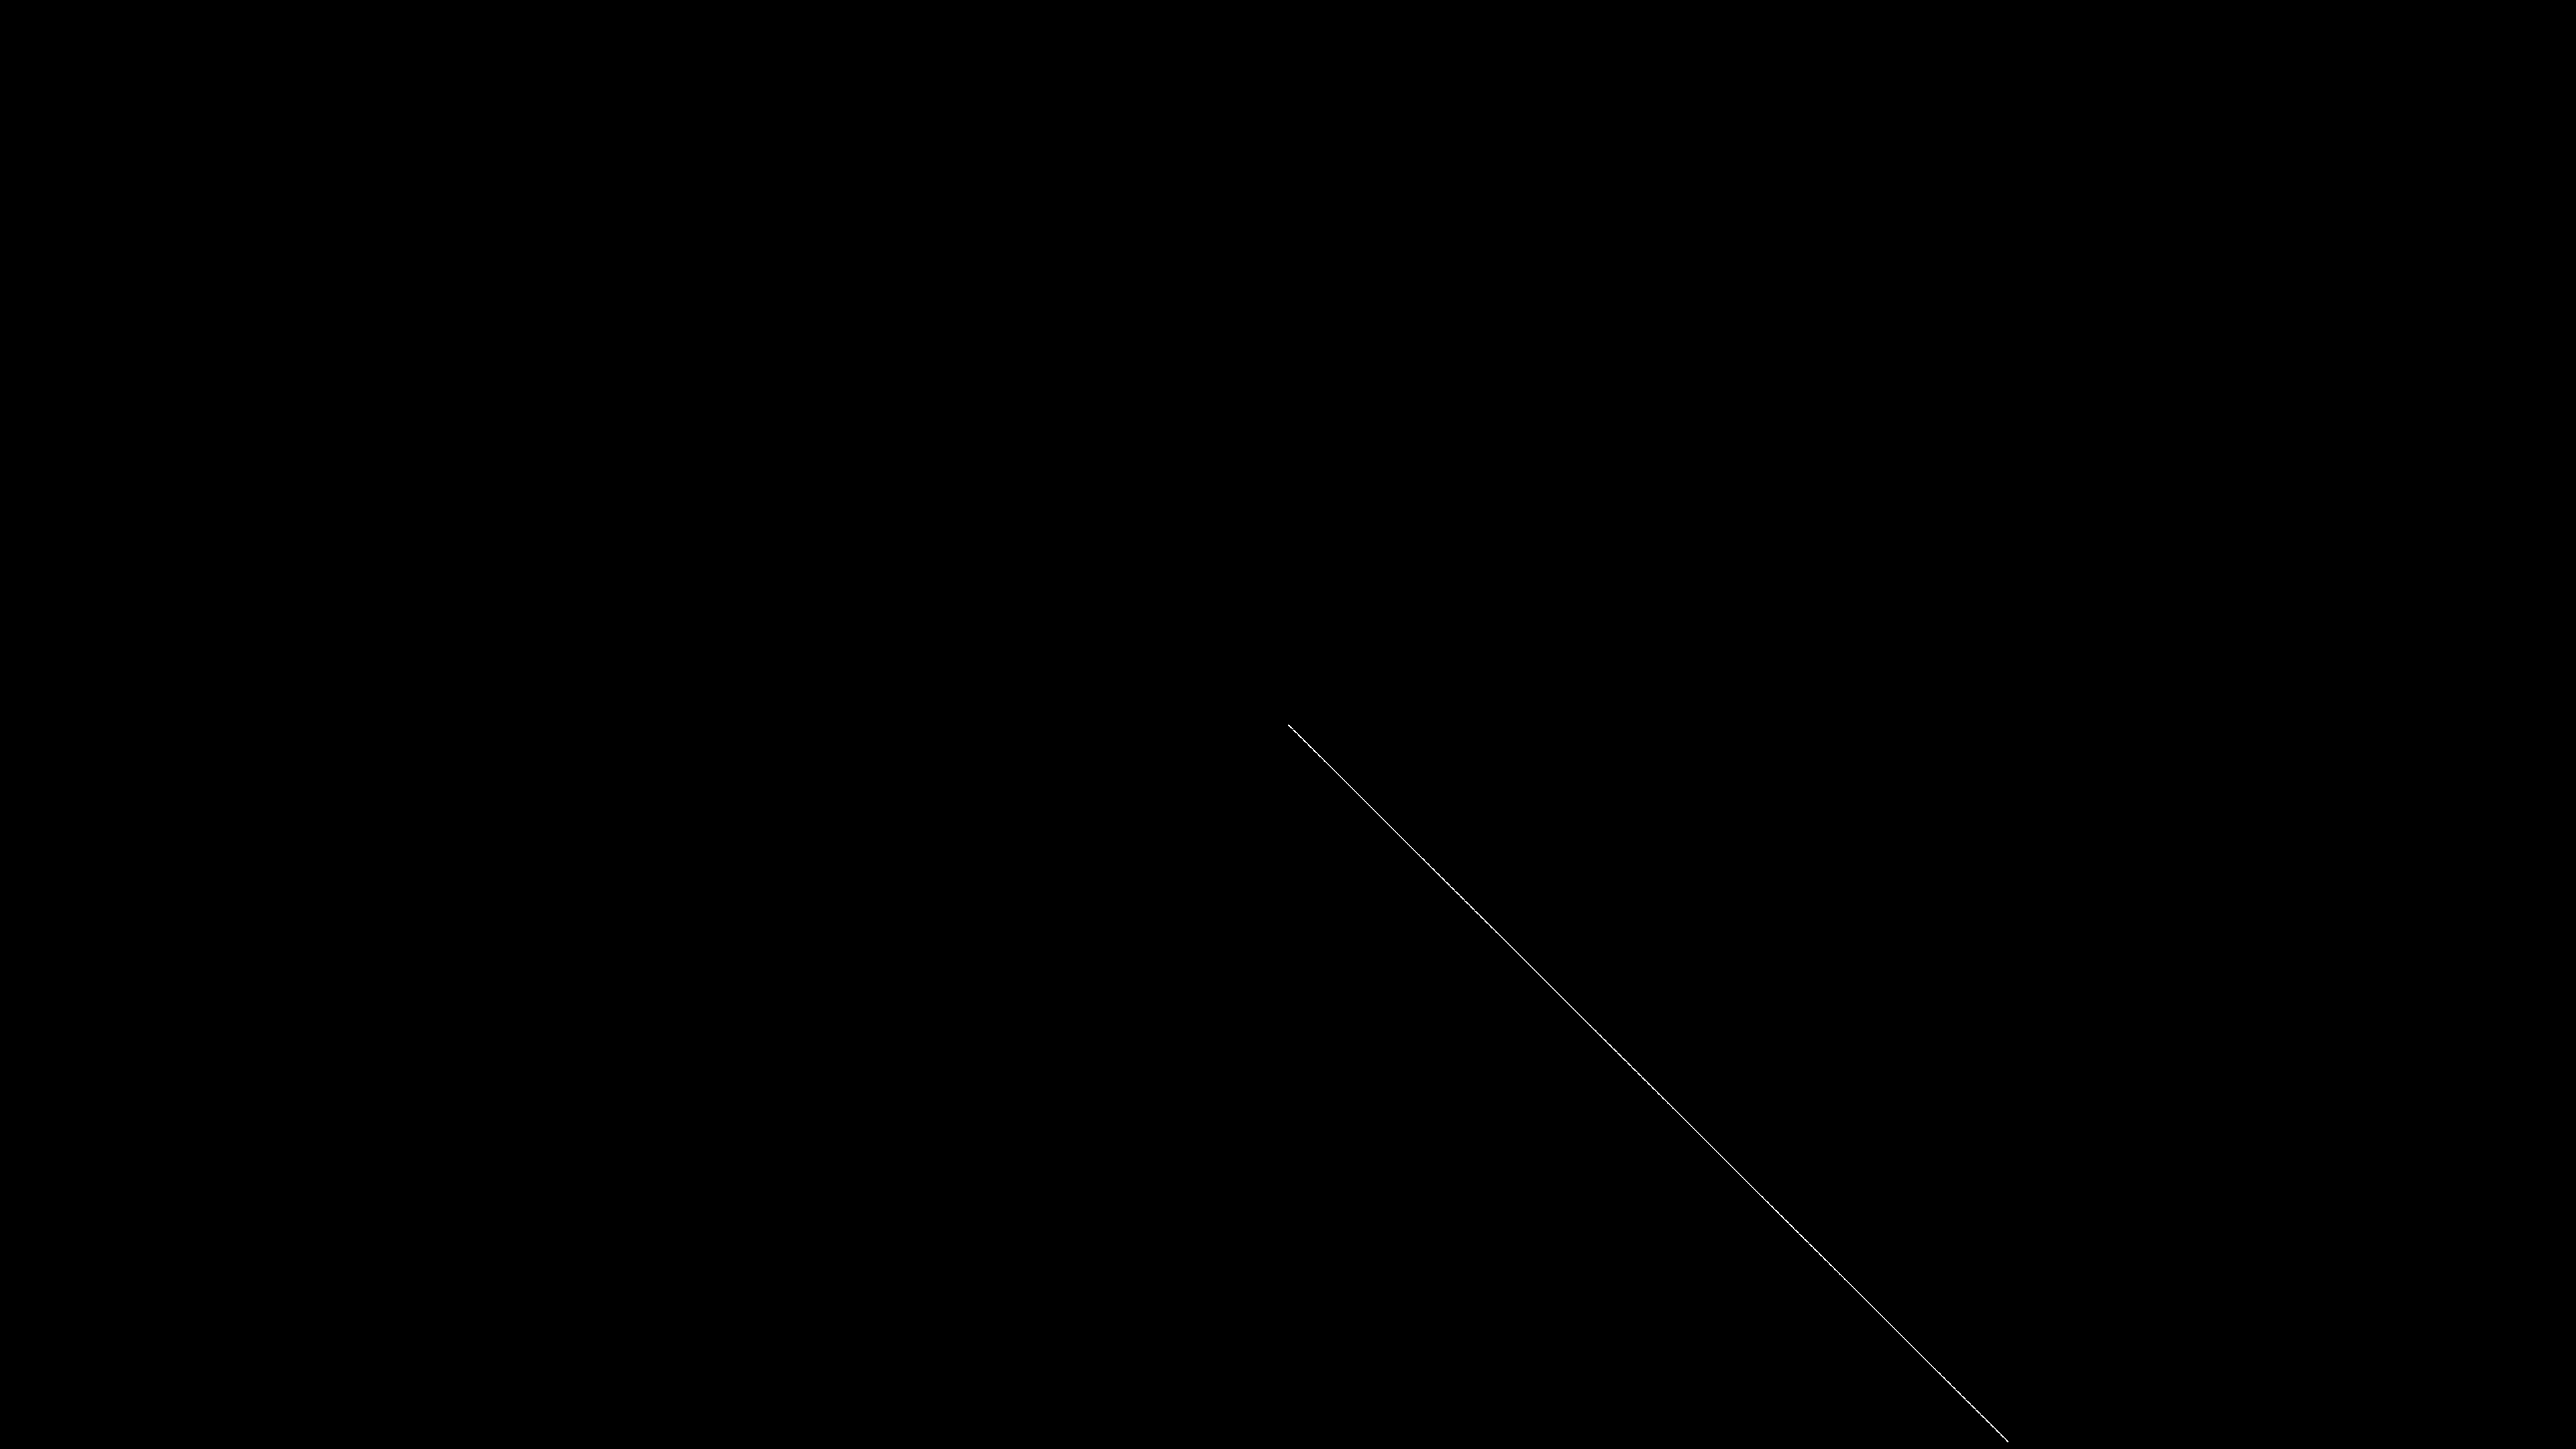
\includegraphics[width=\linewidth]{./stepsplusoneimages/0000000002.png}
    \caption{tf p=499 q=200099 theta=000 89775561.png}
  \end{subfigure}
  \caption{n=000 s=400 s+1=401}
  \label{fig:n=000}
\end{figure}
\begin{figure}[H]
  \centering
  \begin{subfigure}[t]{0.48\textwidth}
    \centering
    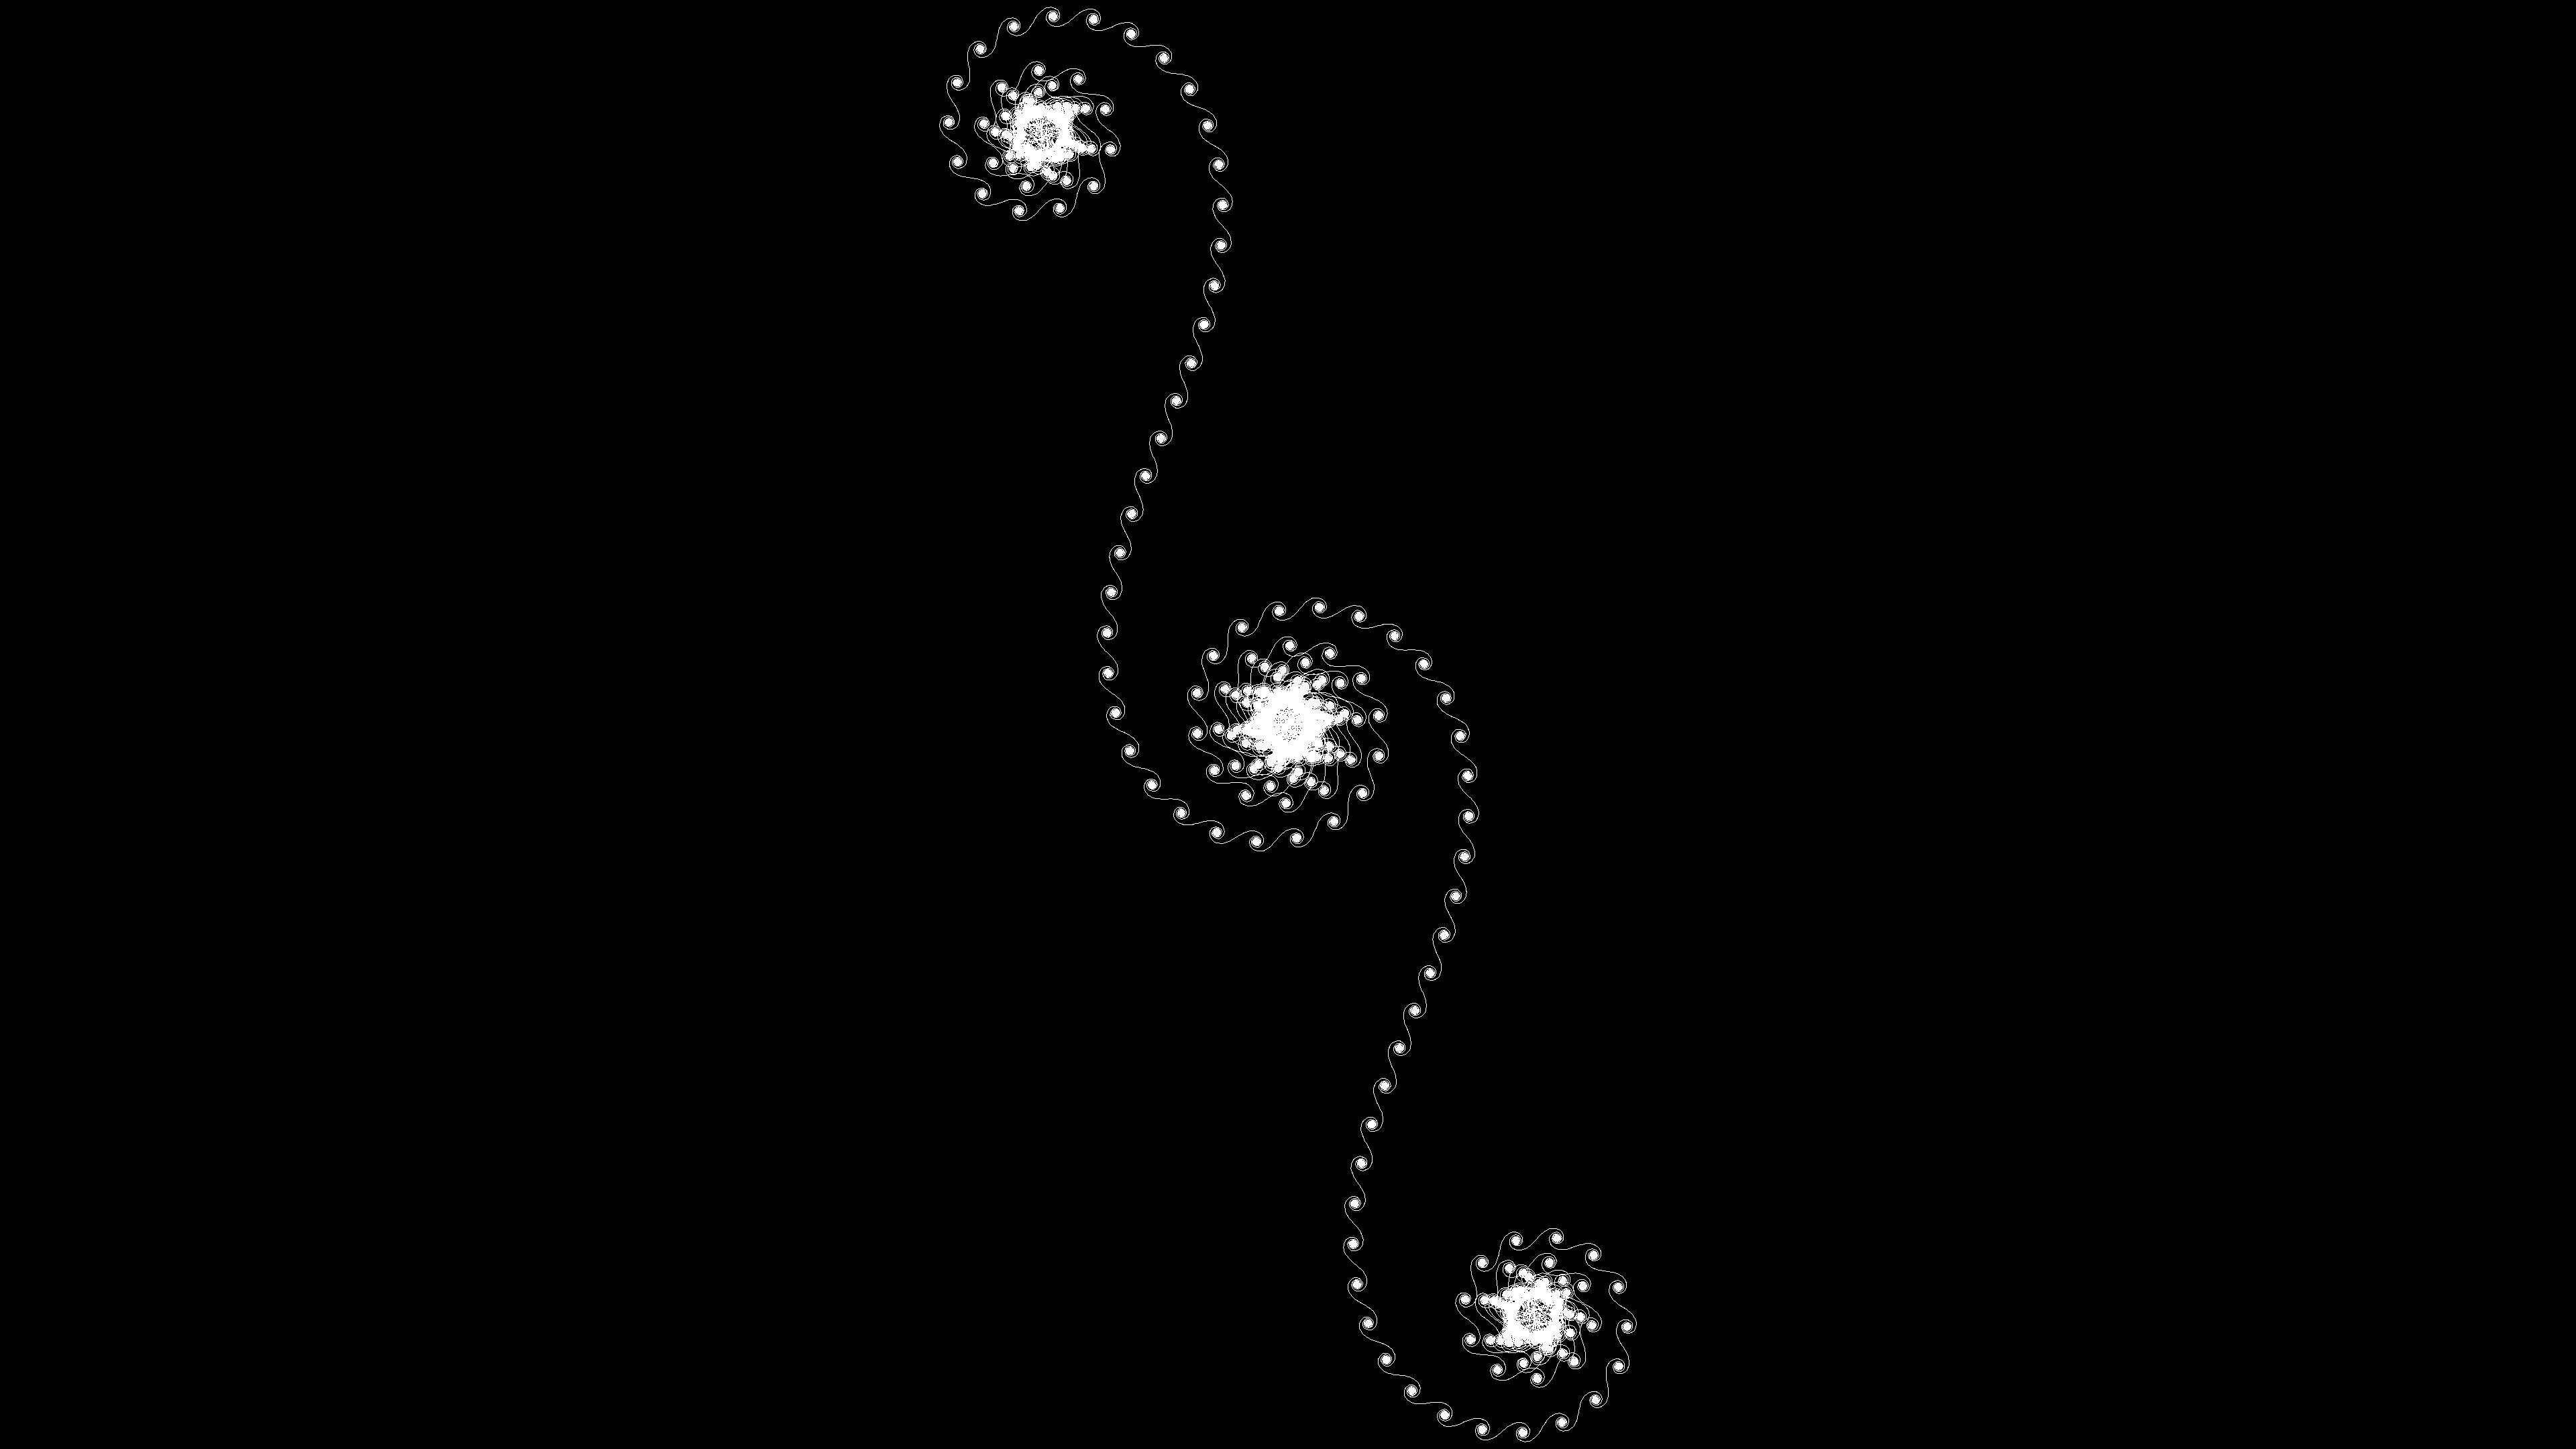
\includegraphics[width=\linewidth]{./stepsplusoneimages/0000000003.png}
    \caption{tf p=499 q=199602 theta=000 89999098.png}
  \end{subfigure}
  \begin{subfigure}[t]{0.48\textwidth}
    \centering
    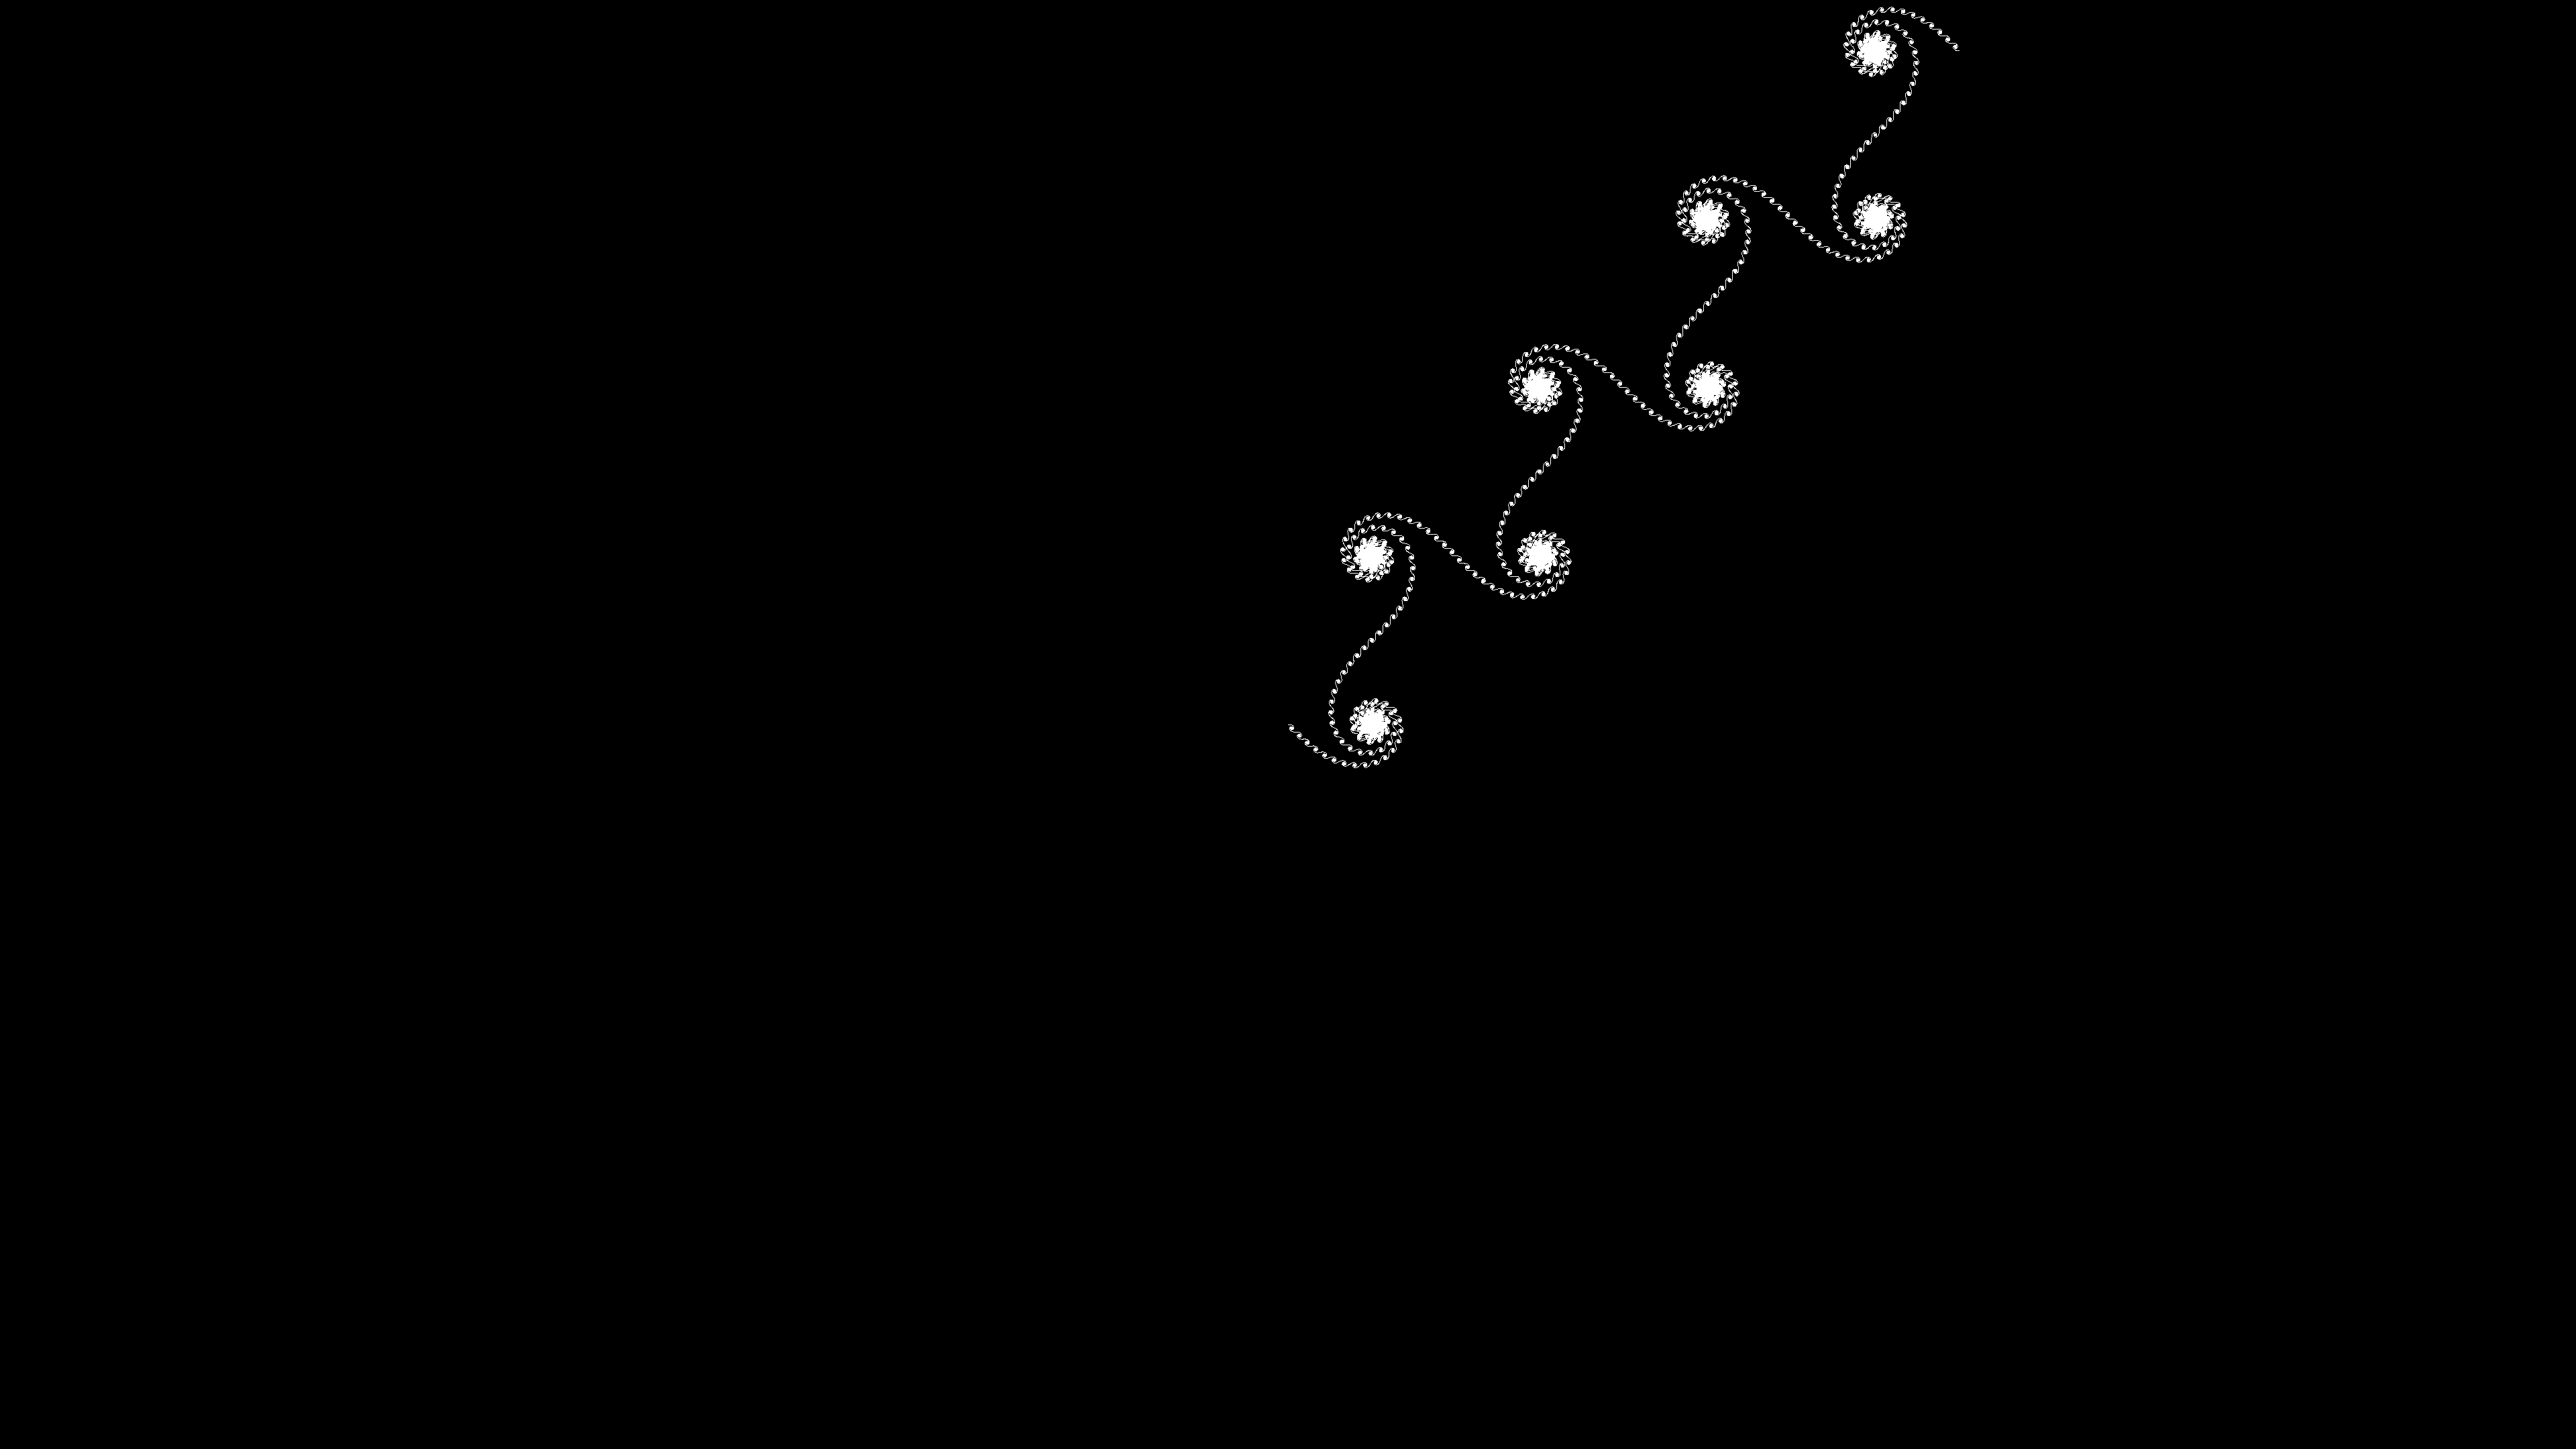
\includegraphics[width=\linewidth]{./stepsplusoneimages/0000000004.png}
    \caption{tf p=499 q=200101 theta=000 89774664.png}
  \end{subfigure}
  \caption{n=002 s=400 s+1=401}
  \label{fig:n=002}
\end{figure}
\begin{figure}[H]
  \centering
  \begin{subfigure}[t]{0.48\textwidth}
    \centering
    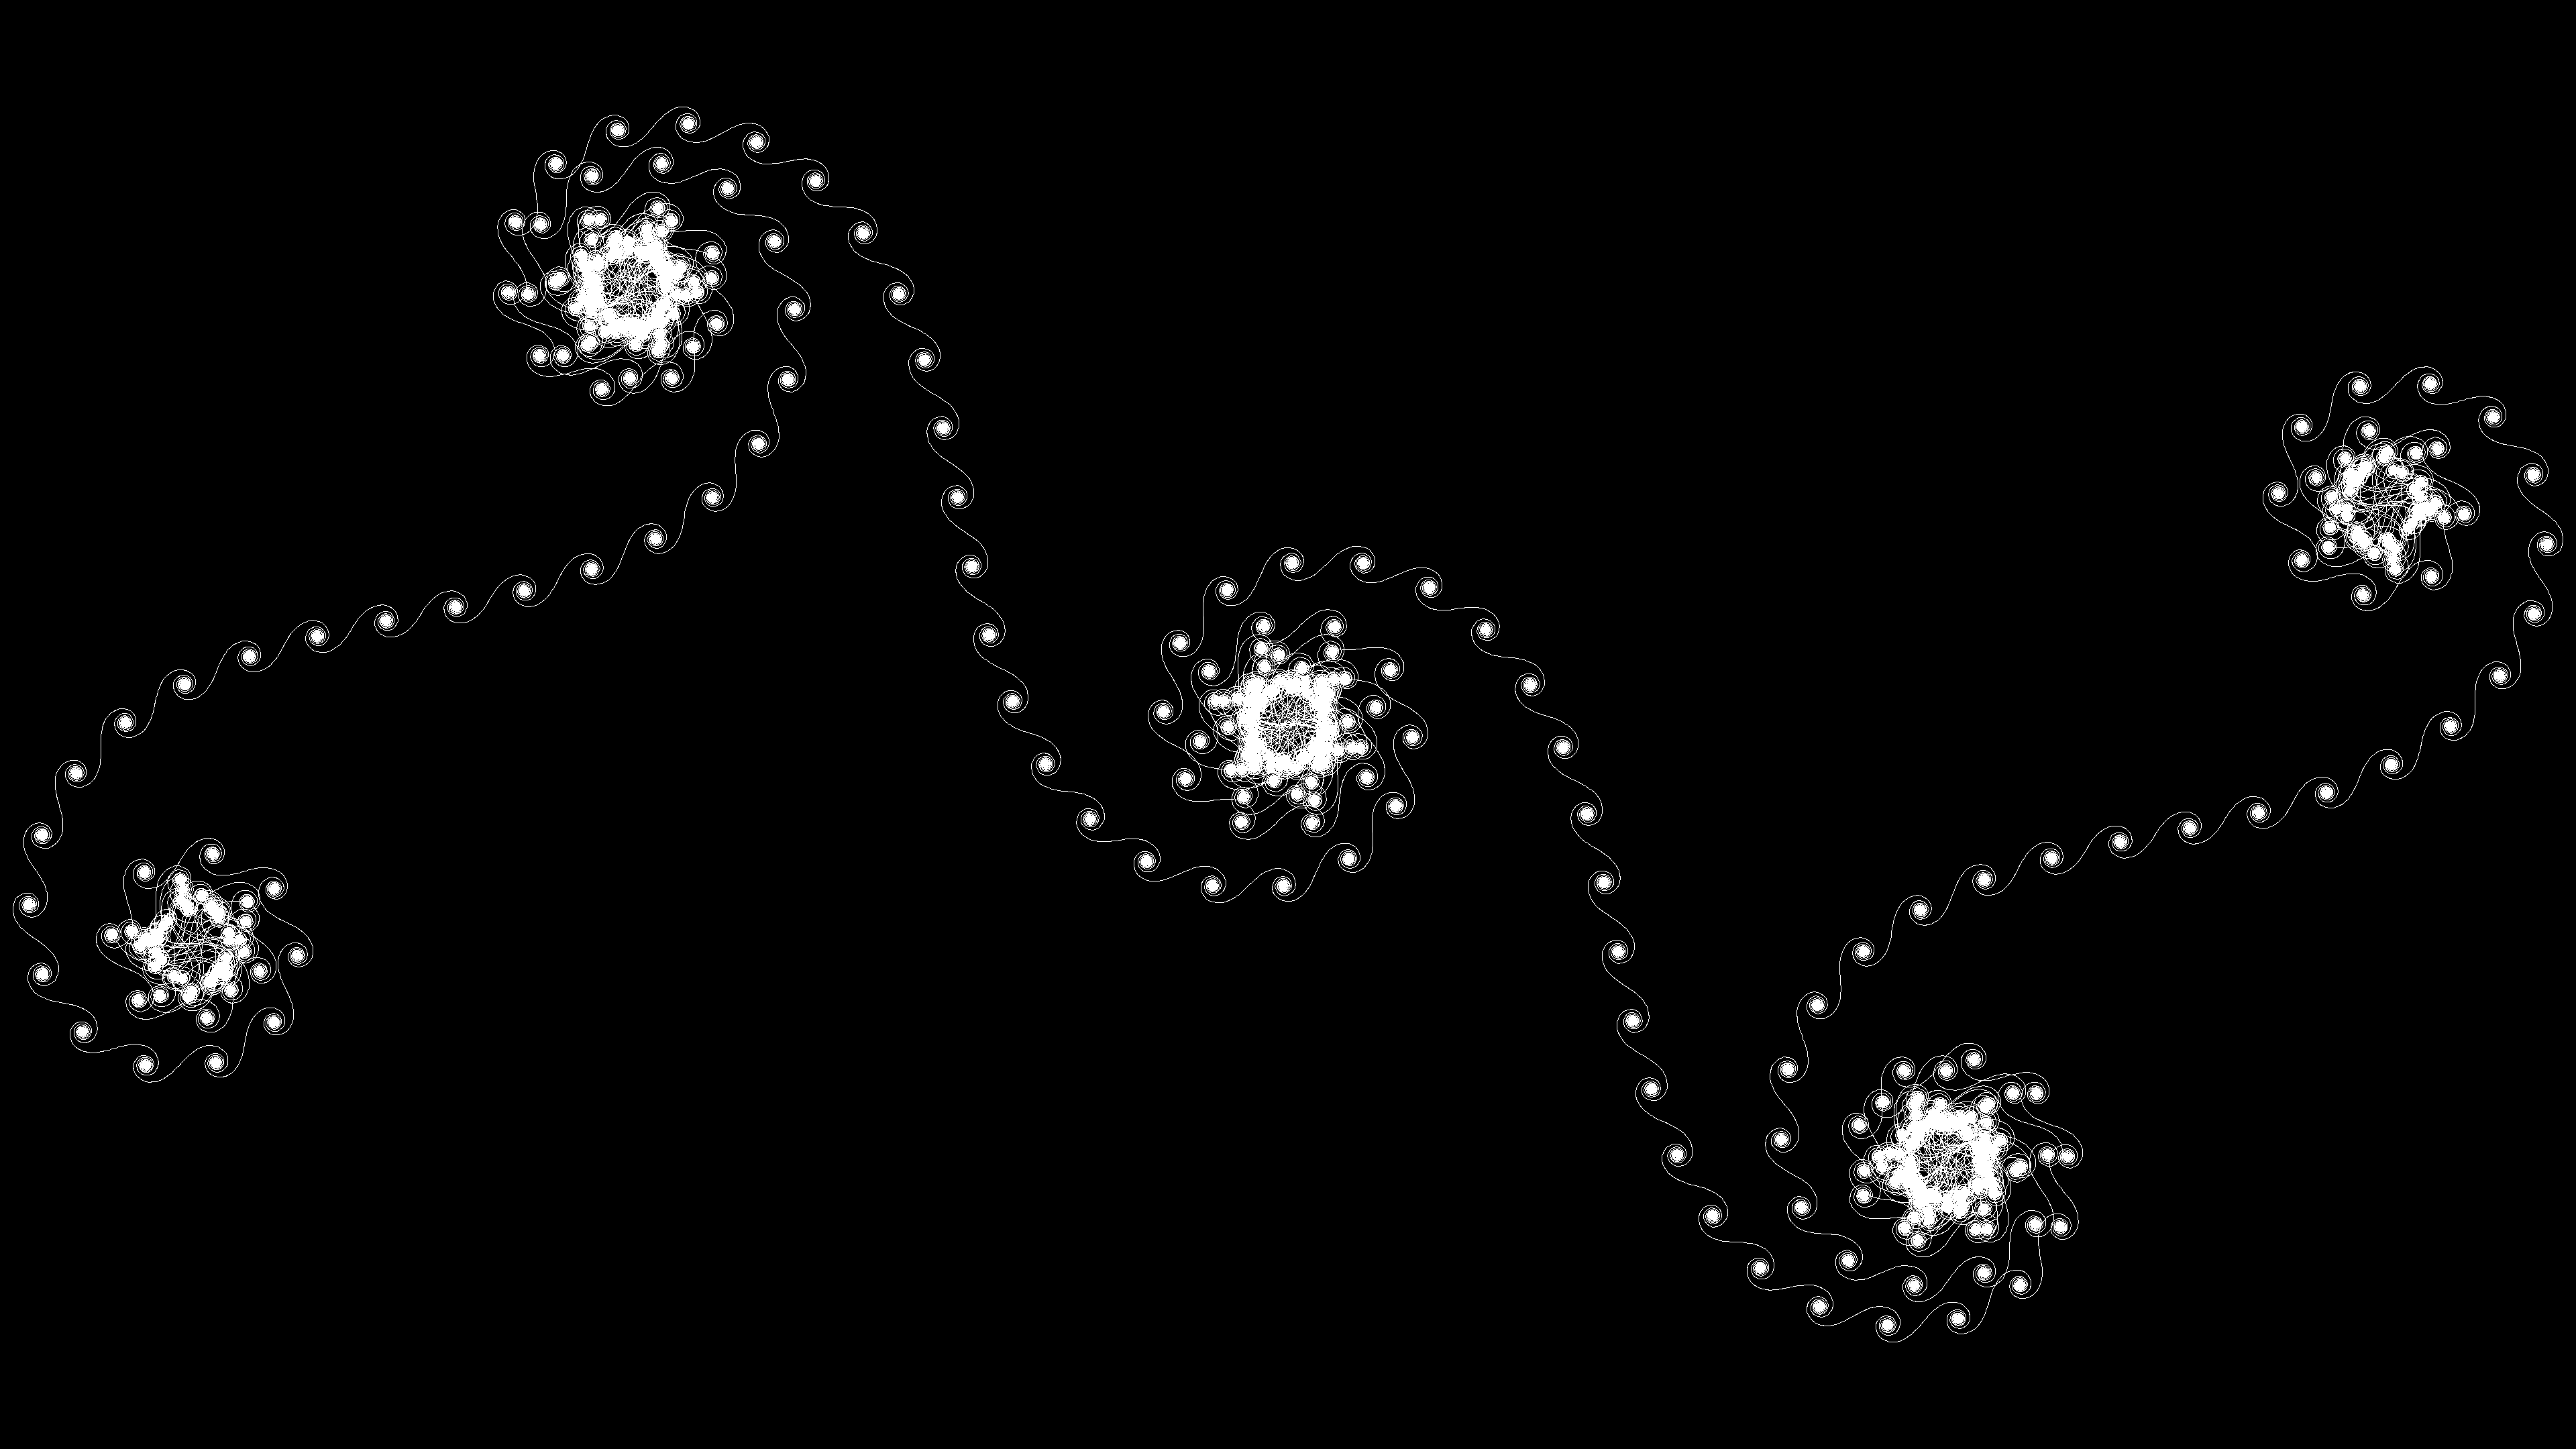
\includegraphics[width=\linewidth]{./stepsplusoneimages/0000000005.png}
    \caption{tf p=499 q=199604 theta=000 89998196.png}
  \end{subfigure}
  \begin{subfigure}[t]{0.48\textwidth}
    \centering
    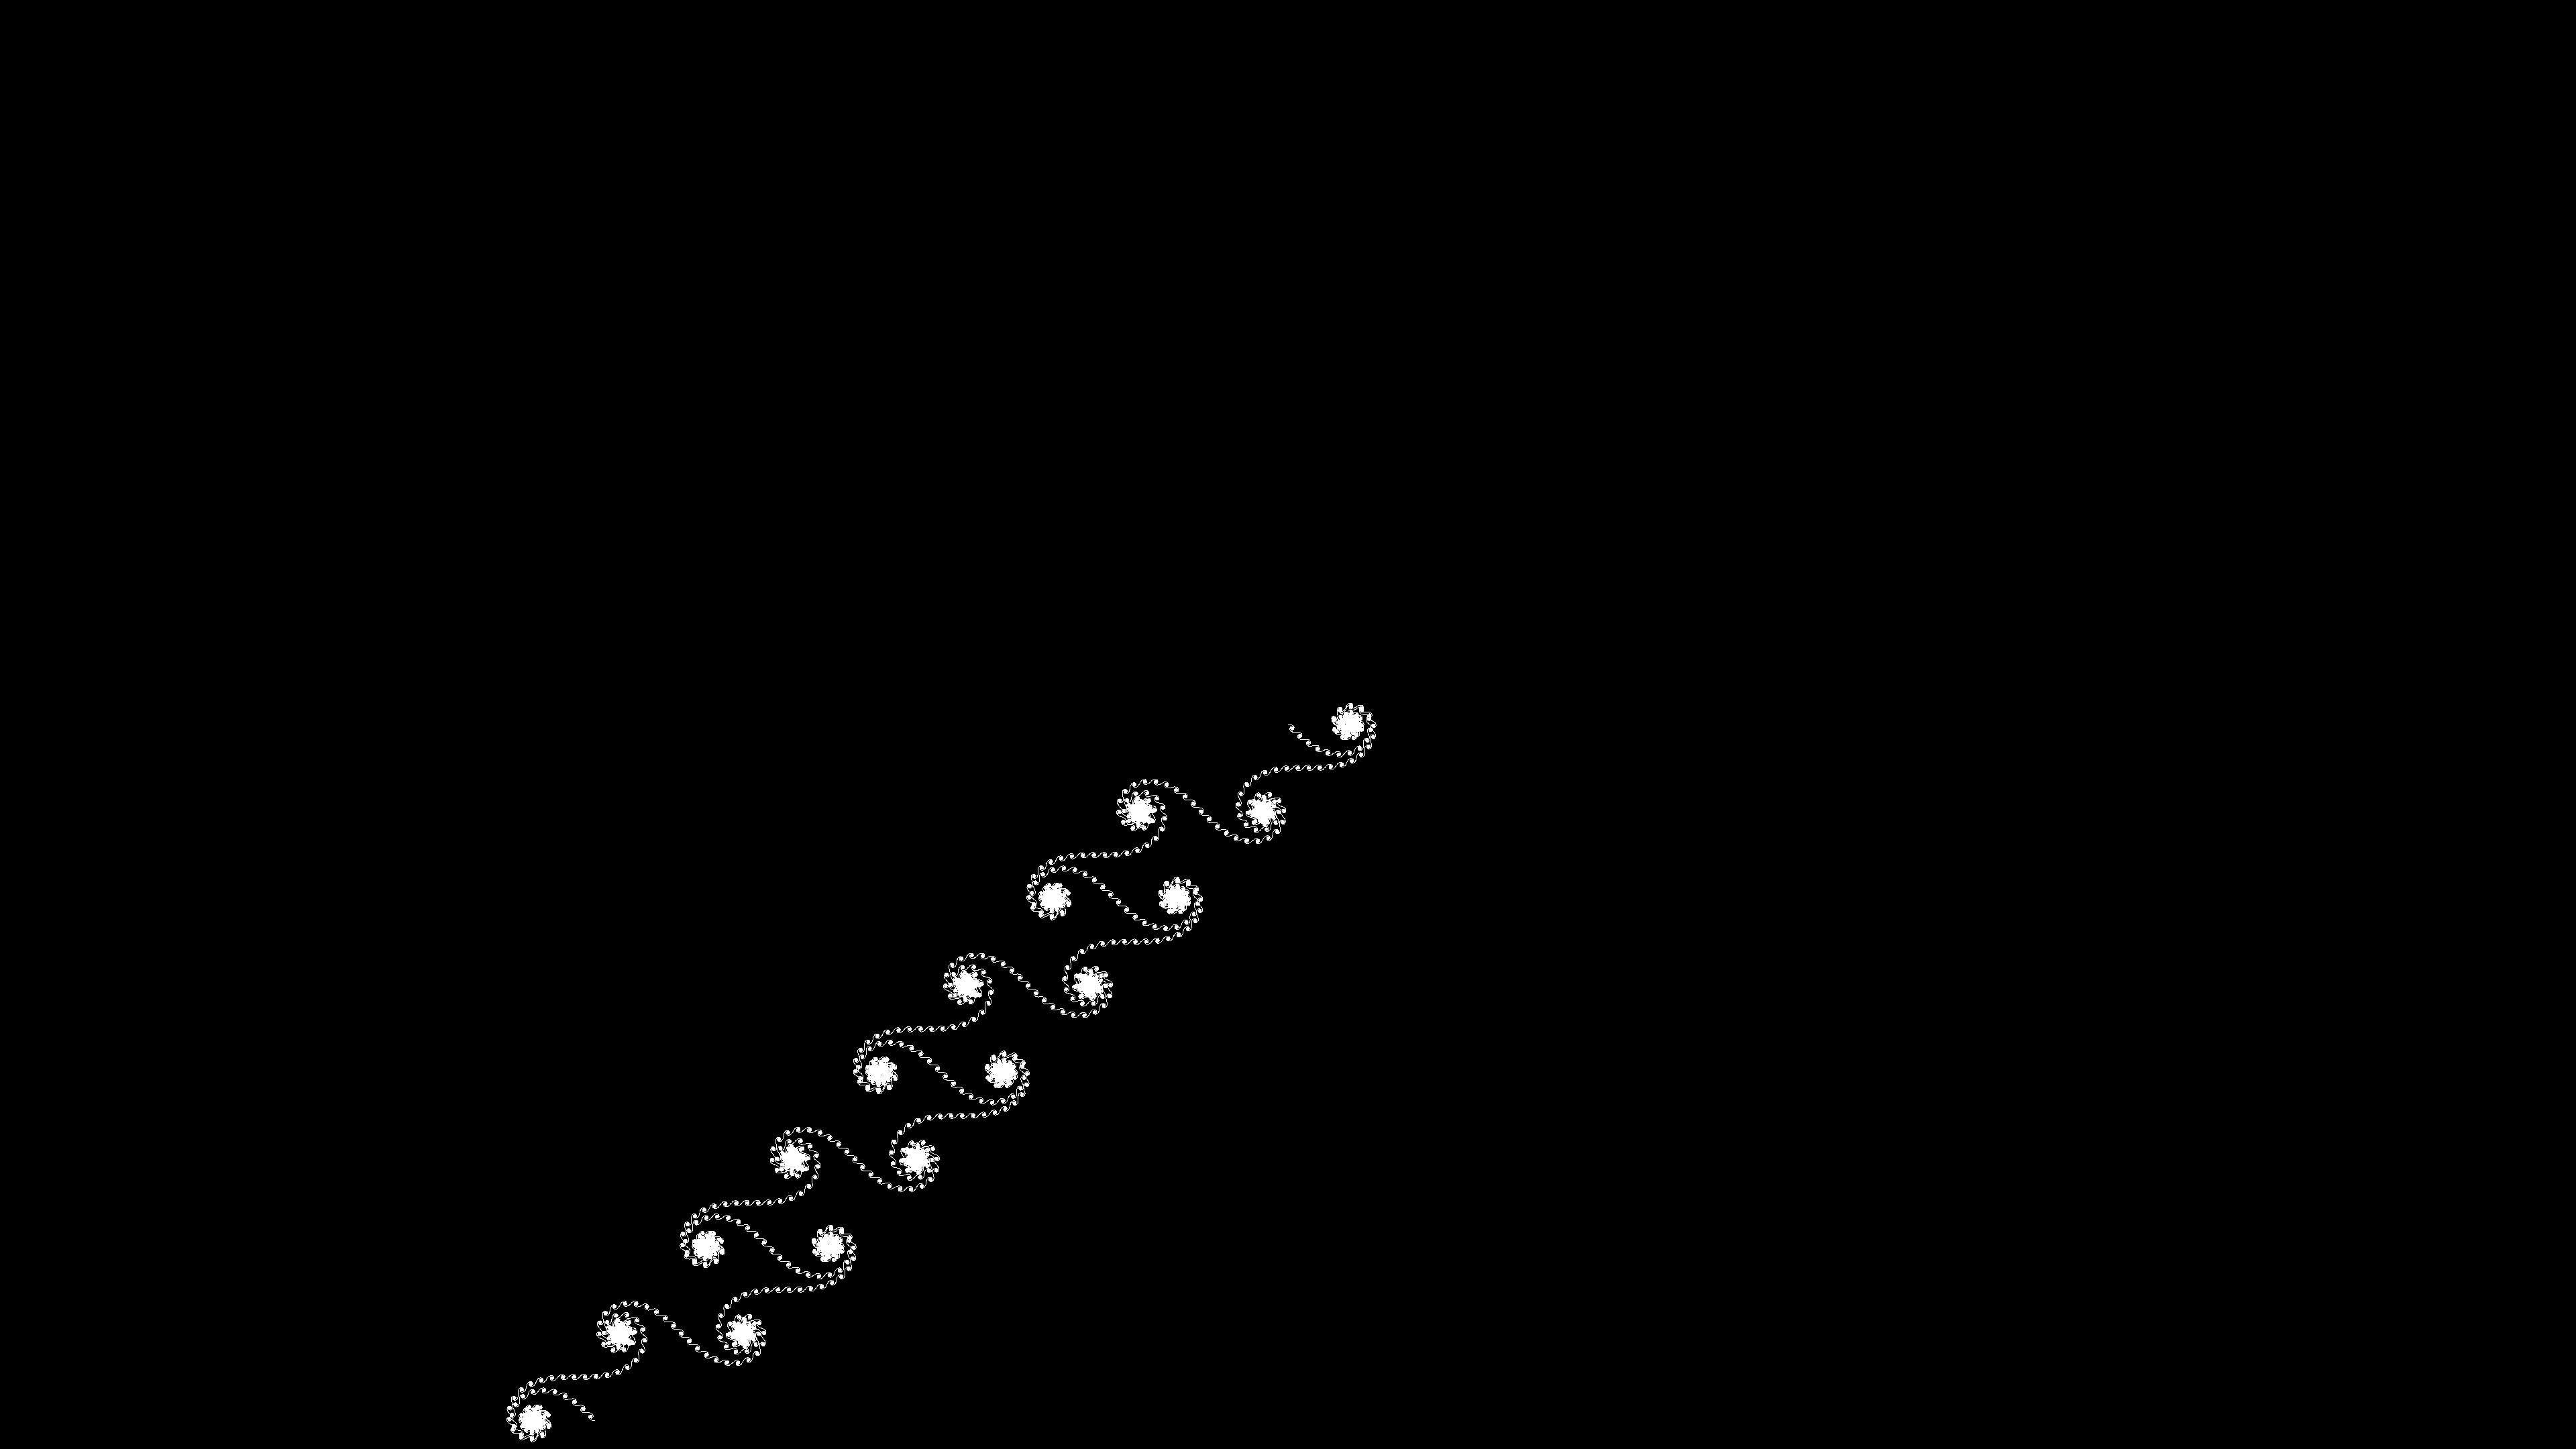
\includegraphics[width=\linewidth]{./stepsplusoneimages/0000000006.png}
    \caption{tf p=499 q=200103 theta=000 89773767.png}
  \end{subfigure}
  \caption{n=004 s=400 s+1=401}
  \label{fig:n=004}
\end{figure}
\begin{figure}[H]
  \centering
  \begin{subfigure}[t]{0.48\textwidth}
    \centering
    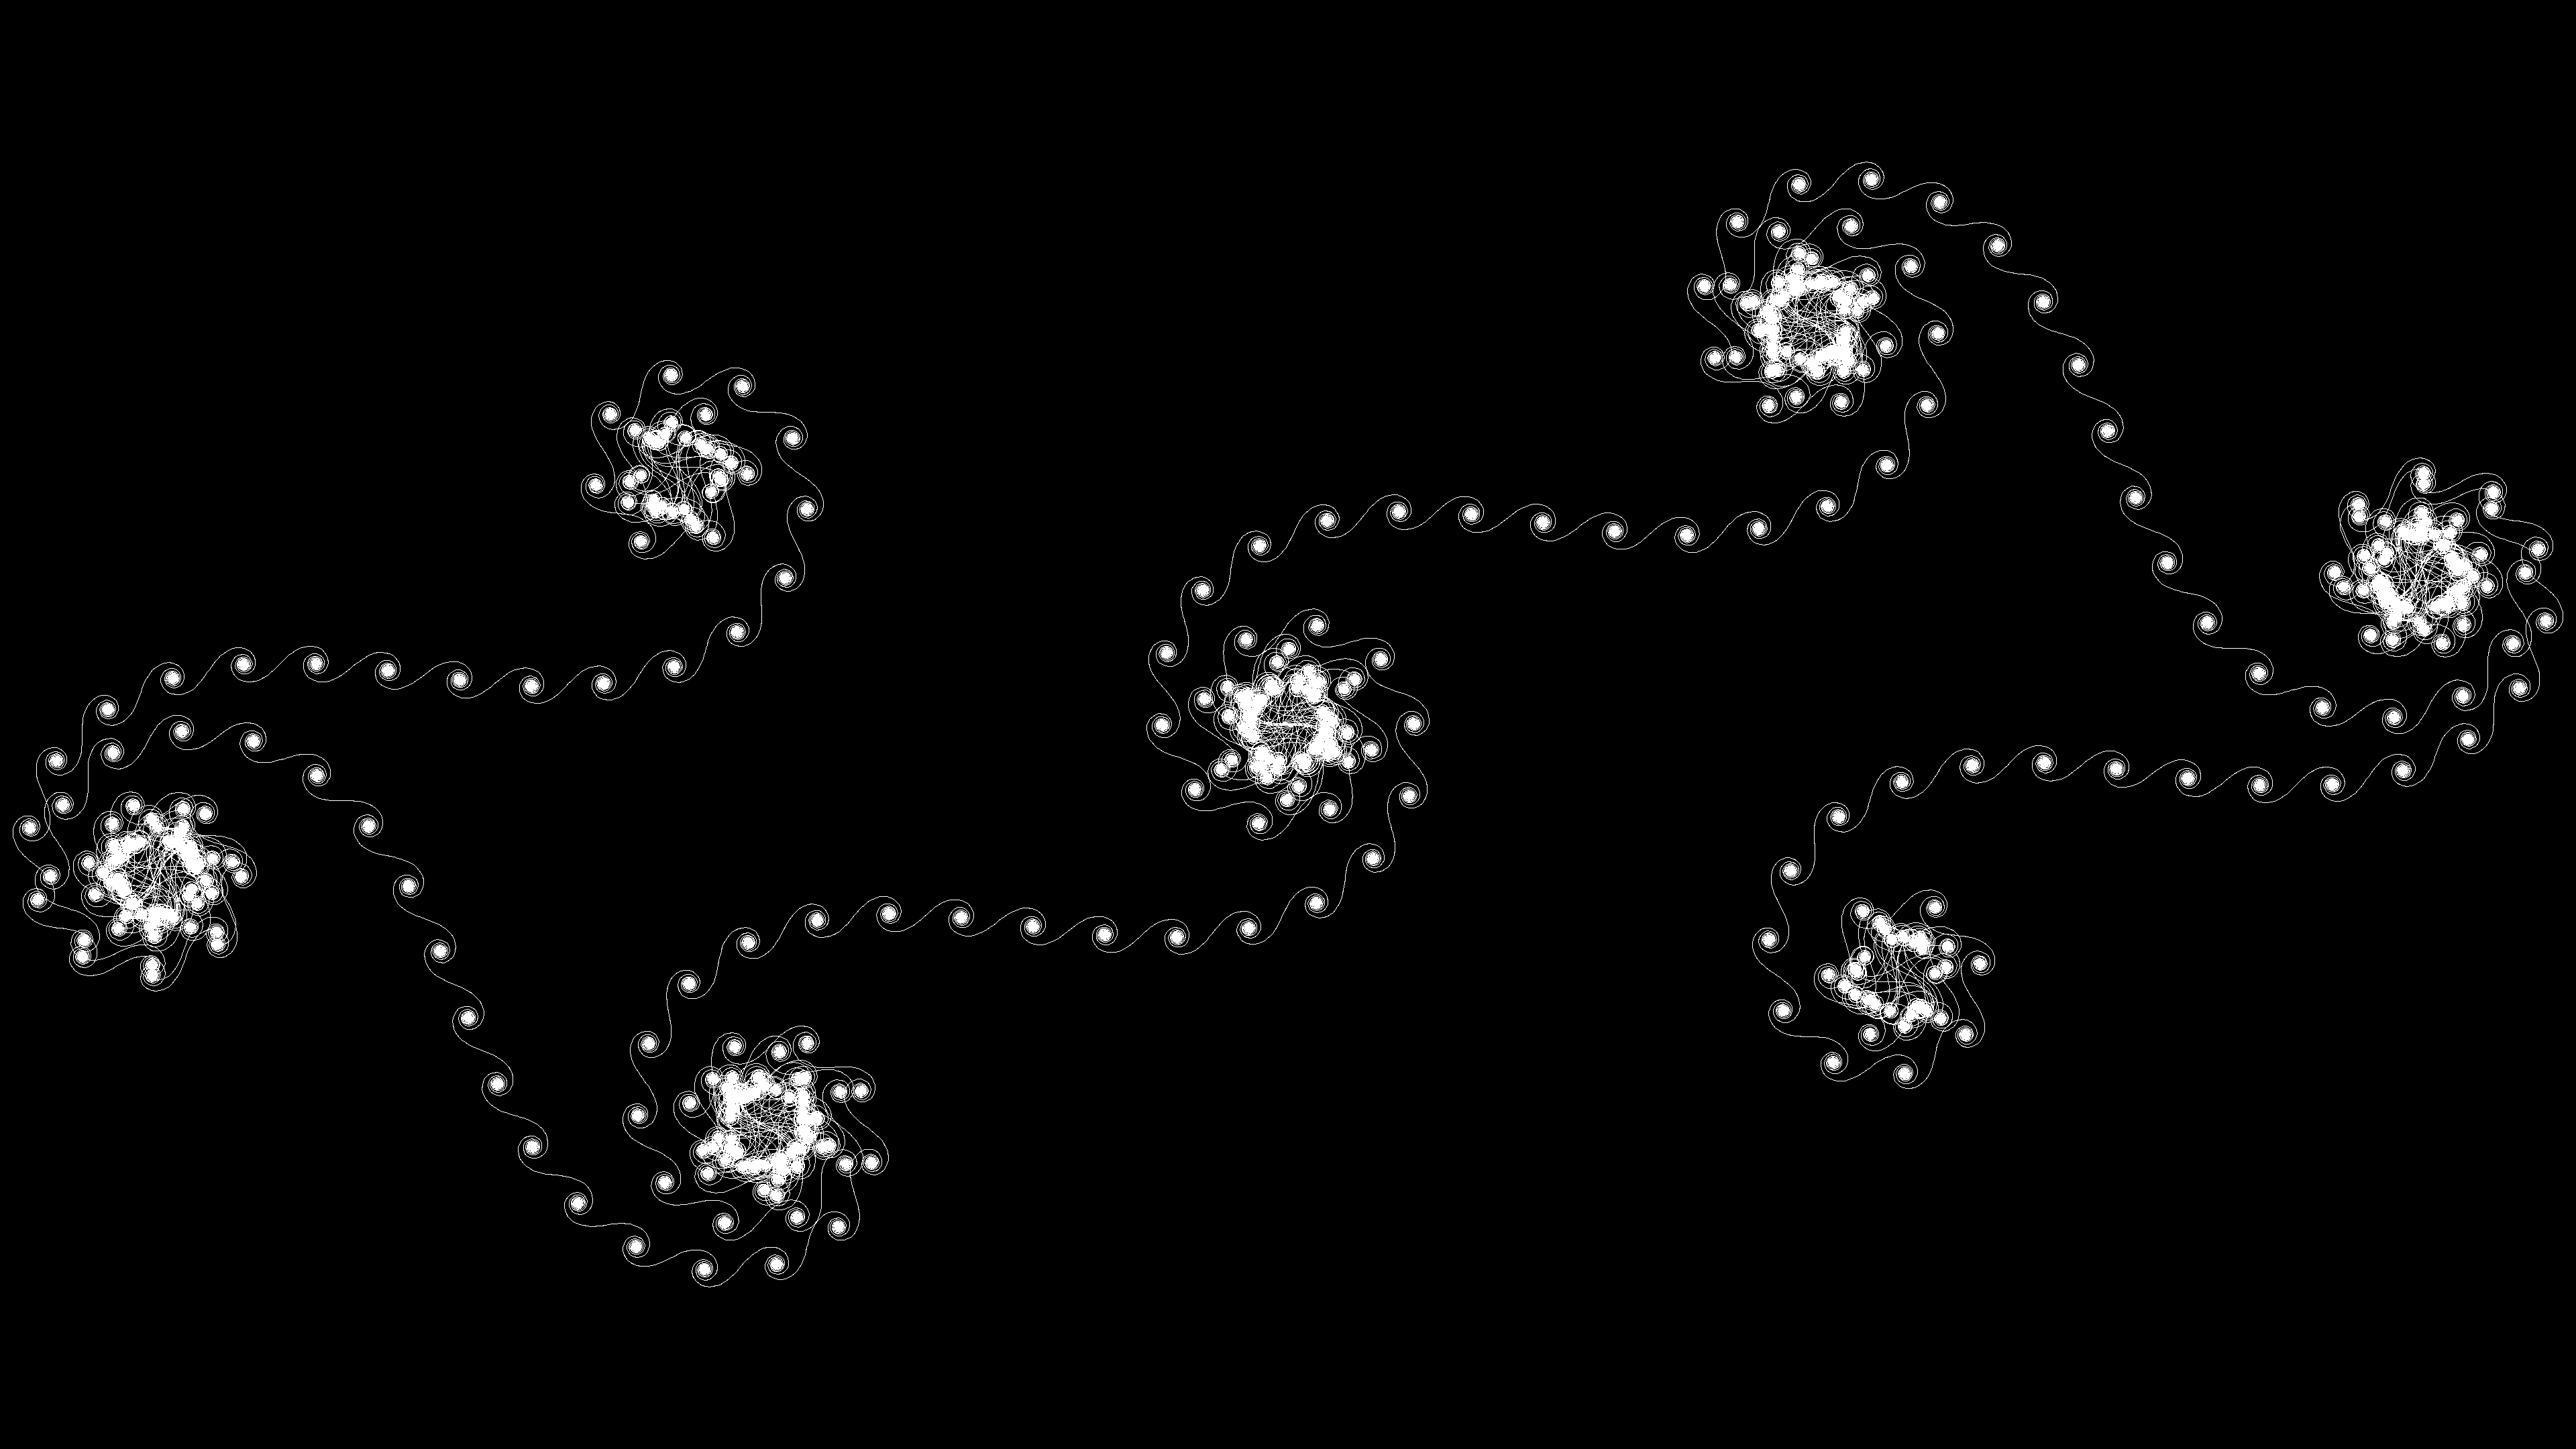
\includegraphics[width=\linewidth]{./stepsplusoneimages/0000000007.png}
    \caption{tf p=499 q=199606 theta=000 89997295.png}
  \end{subfigure}
  \begin{subfigure}[t]{0.48\textwidth}
    \centering
    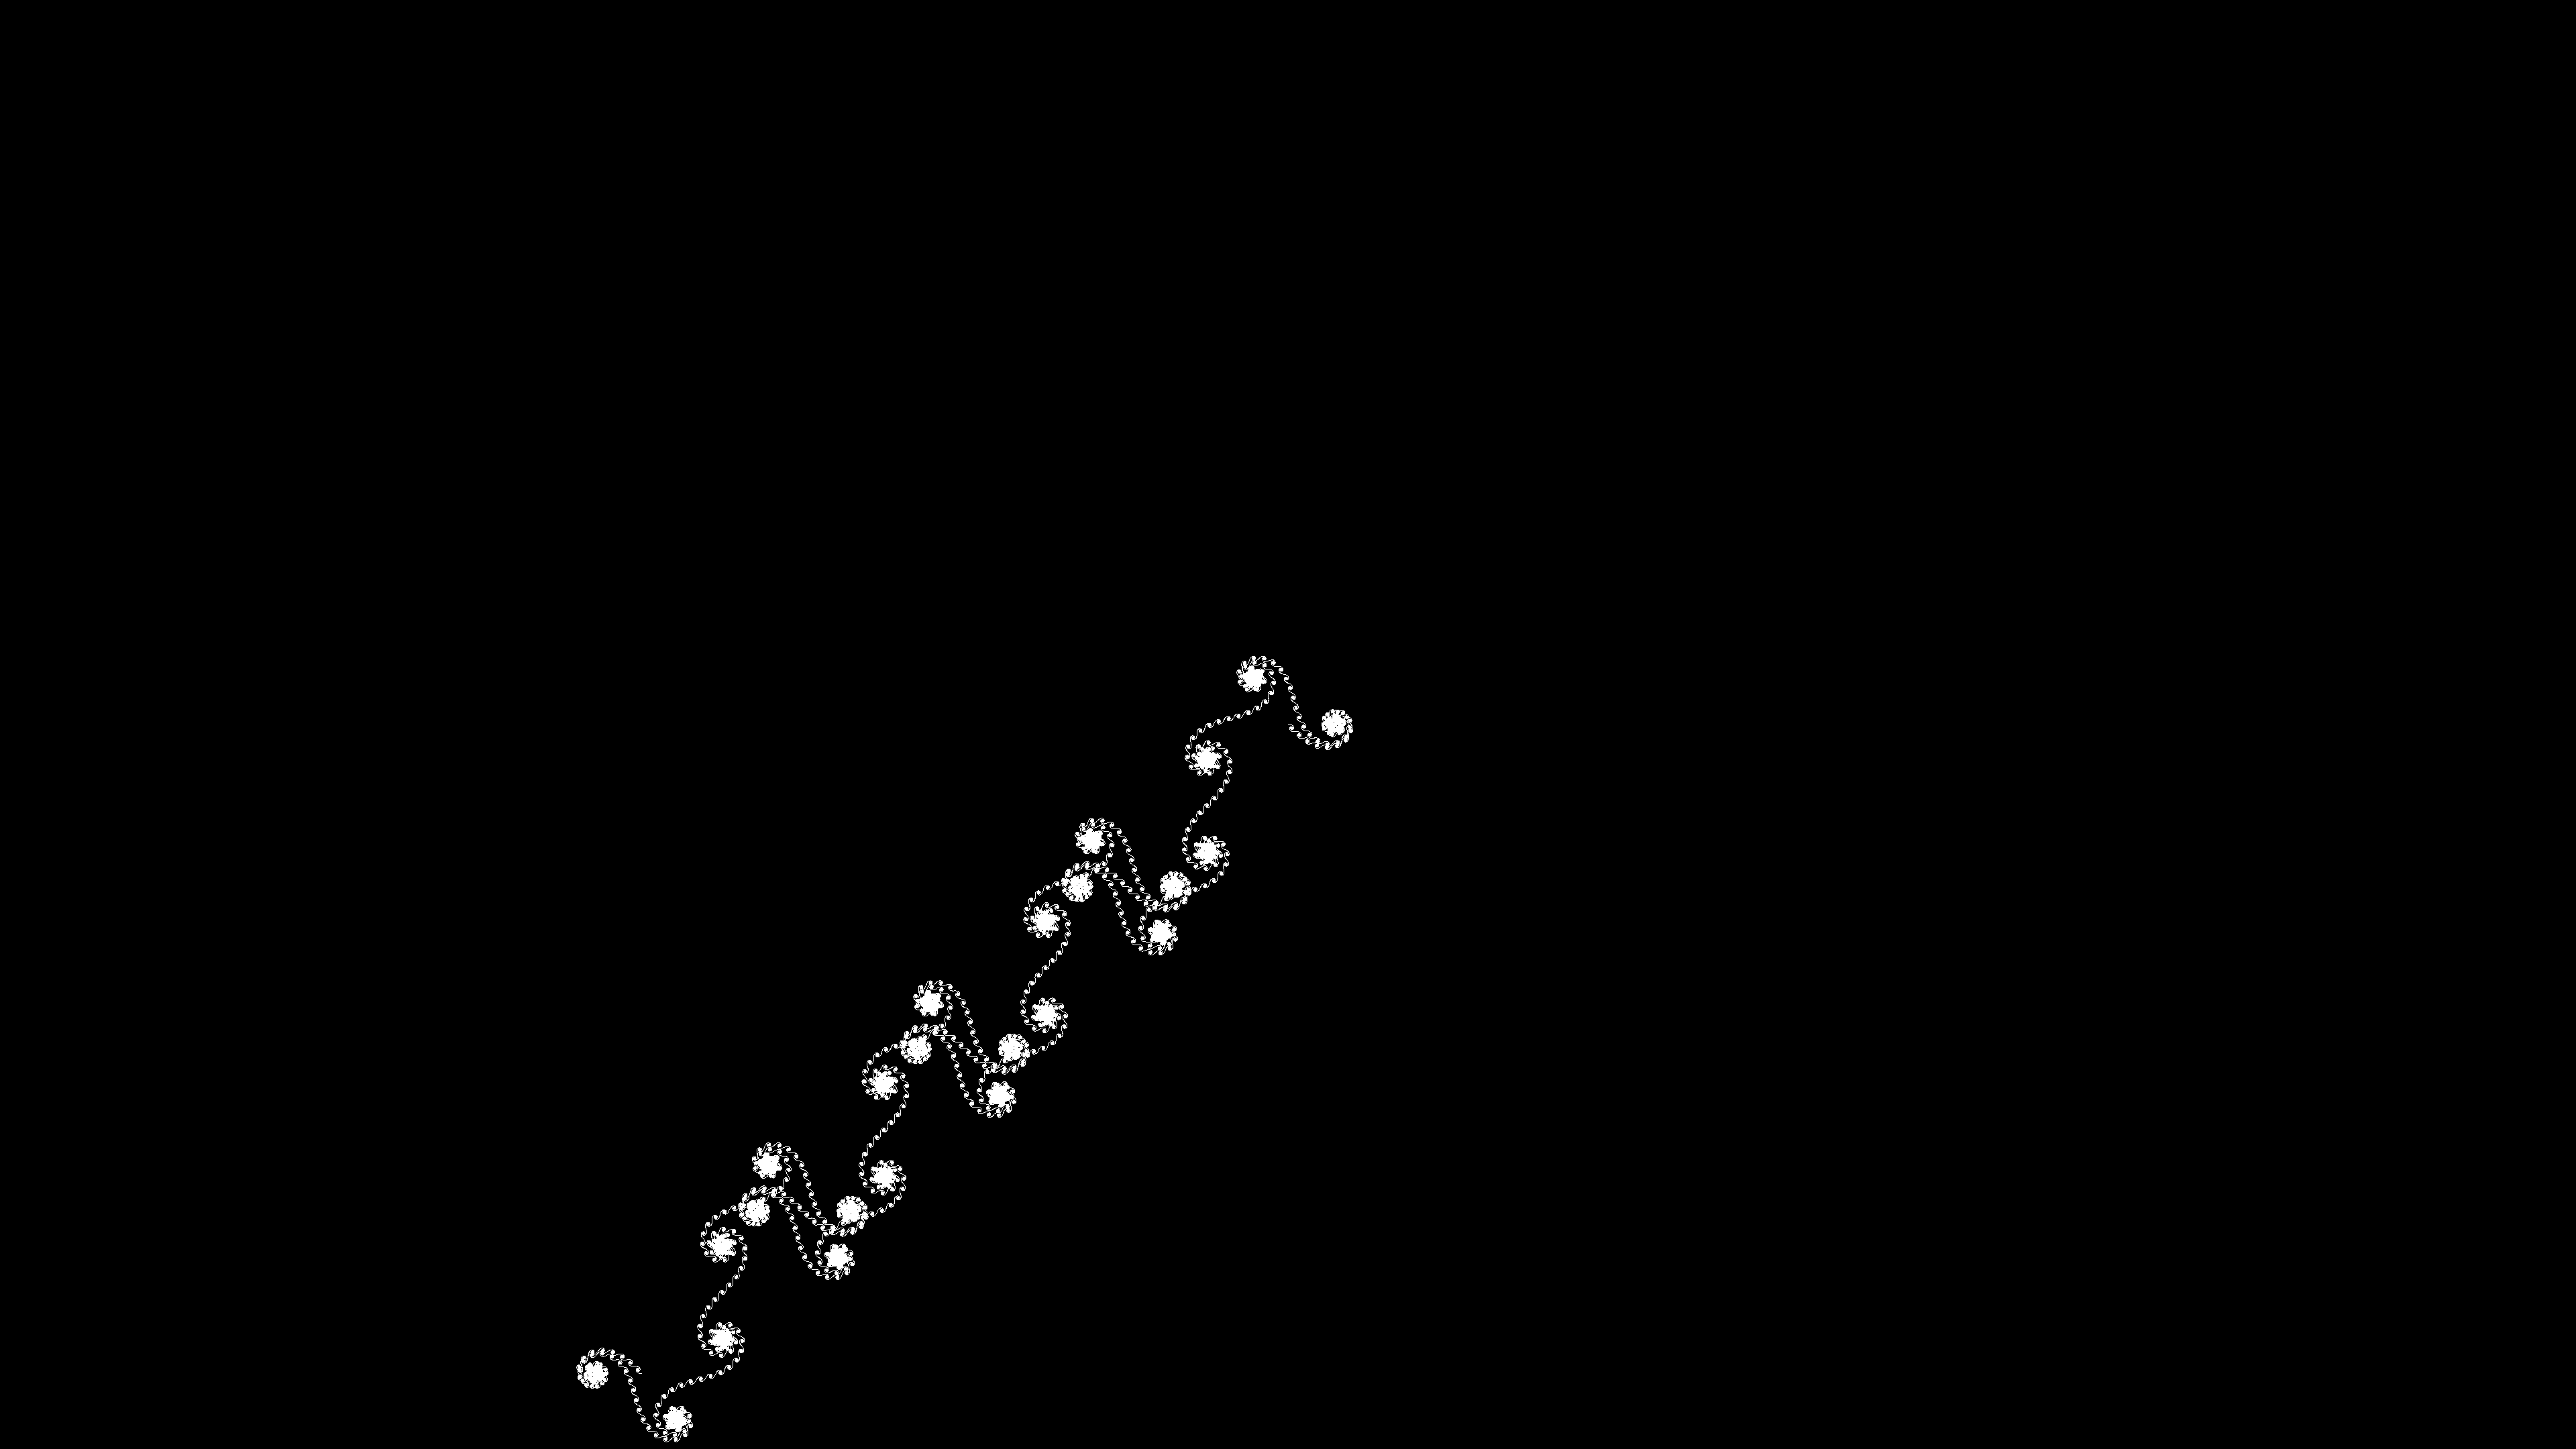
\includegraphics[width=\linewidth]{./stepsplusoneimages/0000000008.png}
    \caption{tf p=499 q=200105 theta=000 89772869.png}
  \end{subfigure}
  \caption{n=006 s=400 s+1=401}
  \label{fig:n=006}
\end{figure}
\begin{figure}[H]
  \centering
  \begin{subfigure}[t]{0.48\textwidth}
    \centering
    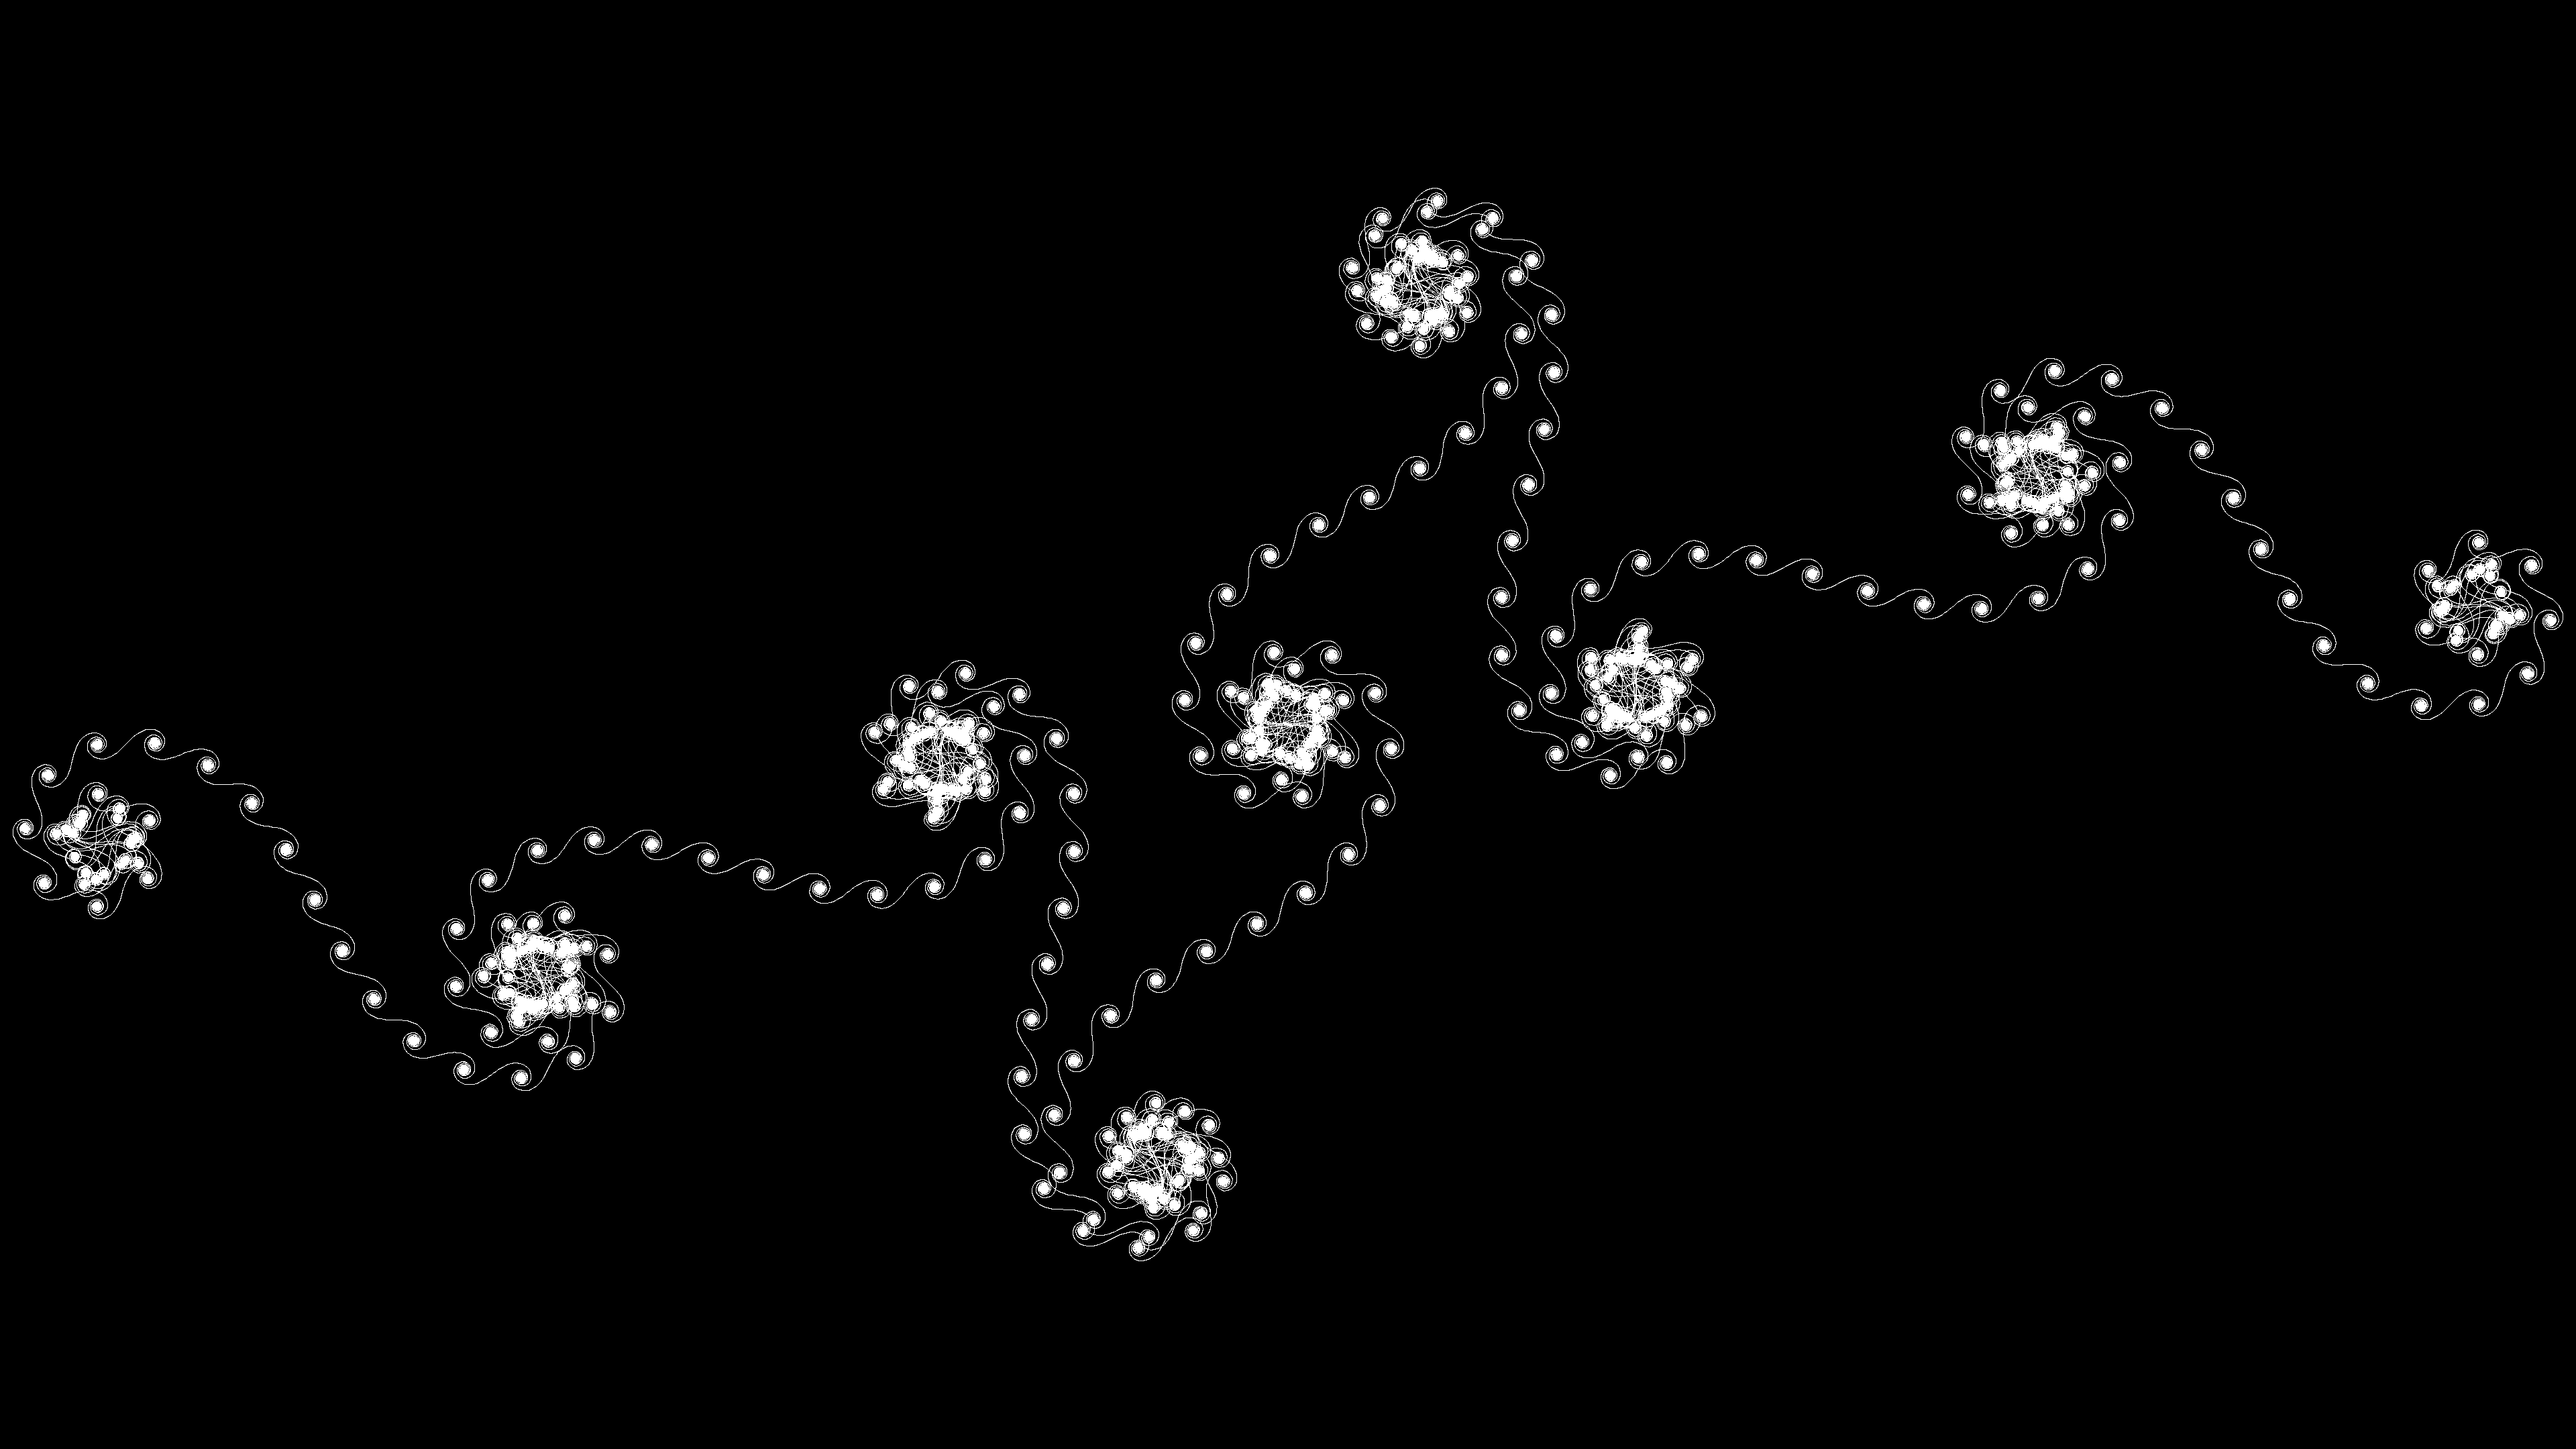
\includegraphics[width=\linewidth]{./stepsplusoneimages/0000000009.png}
    \caption{tf p=499 q=199608 theta=000 89996393.png}
  \end{subfigure}
  \begin{subfigure}[t]{0.48\textwidth}
    \centering
    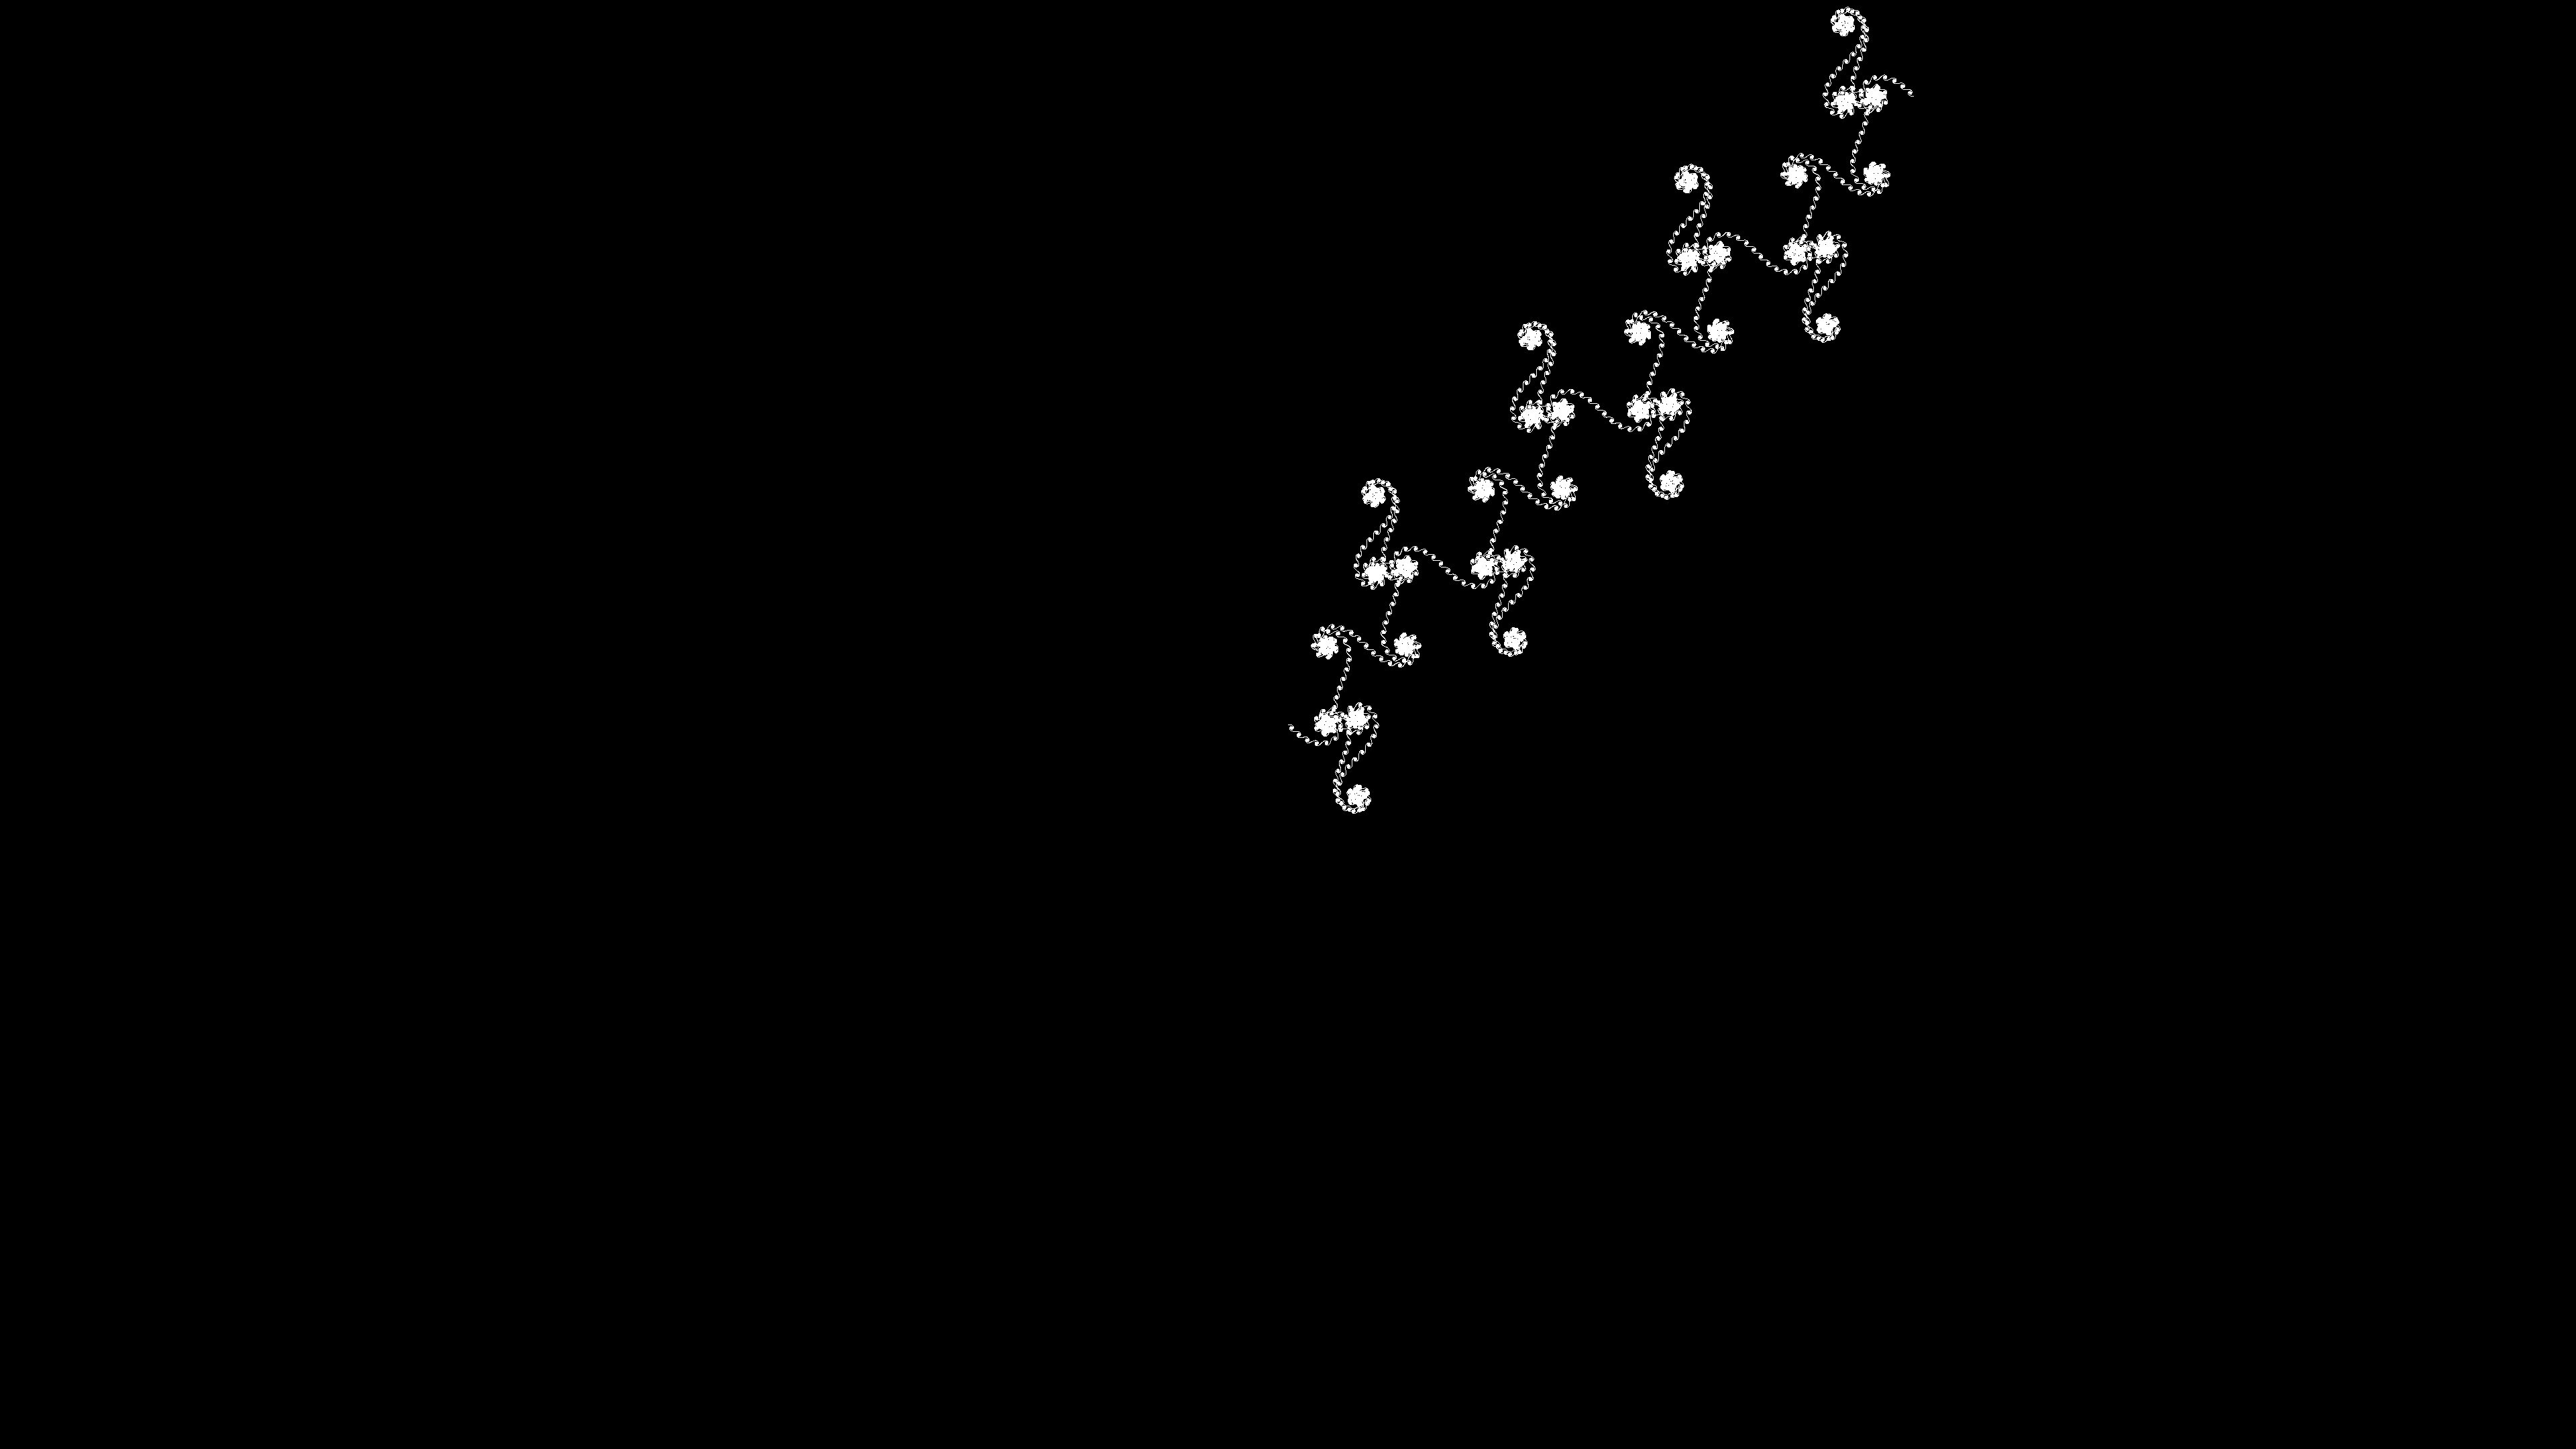
\includegraphics[width=\linewidth]{./stepsplusoneimages/0000000010.png}
    \caption{tf p=499 q=200107 theta=000 89771972.png}
  \end{subfigure}
  \caption{n=008 s=400 s+1=401}
  \label{fig:n=008}
\end{figure}
\begin{figure}[H]
  \centering
  \begin{subfigure}[t]{0.48\textwidth}
    \centering
    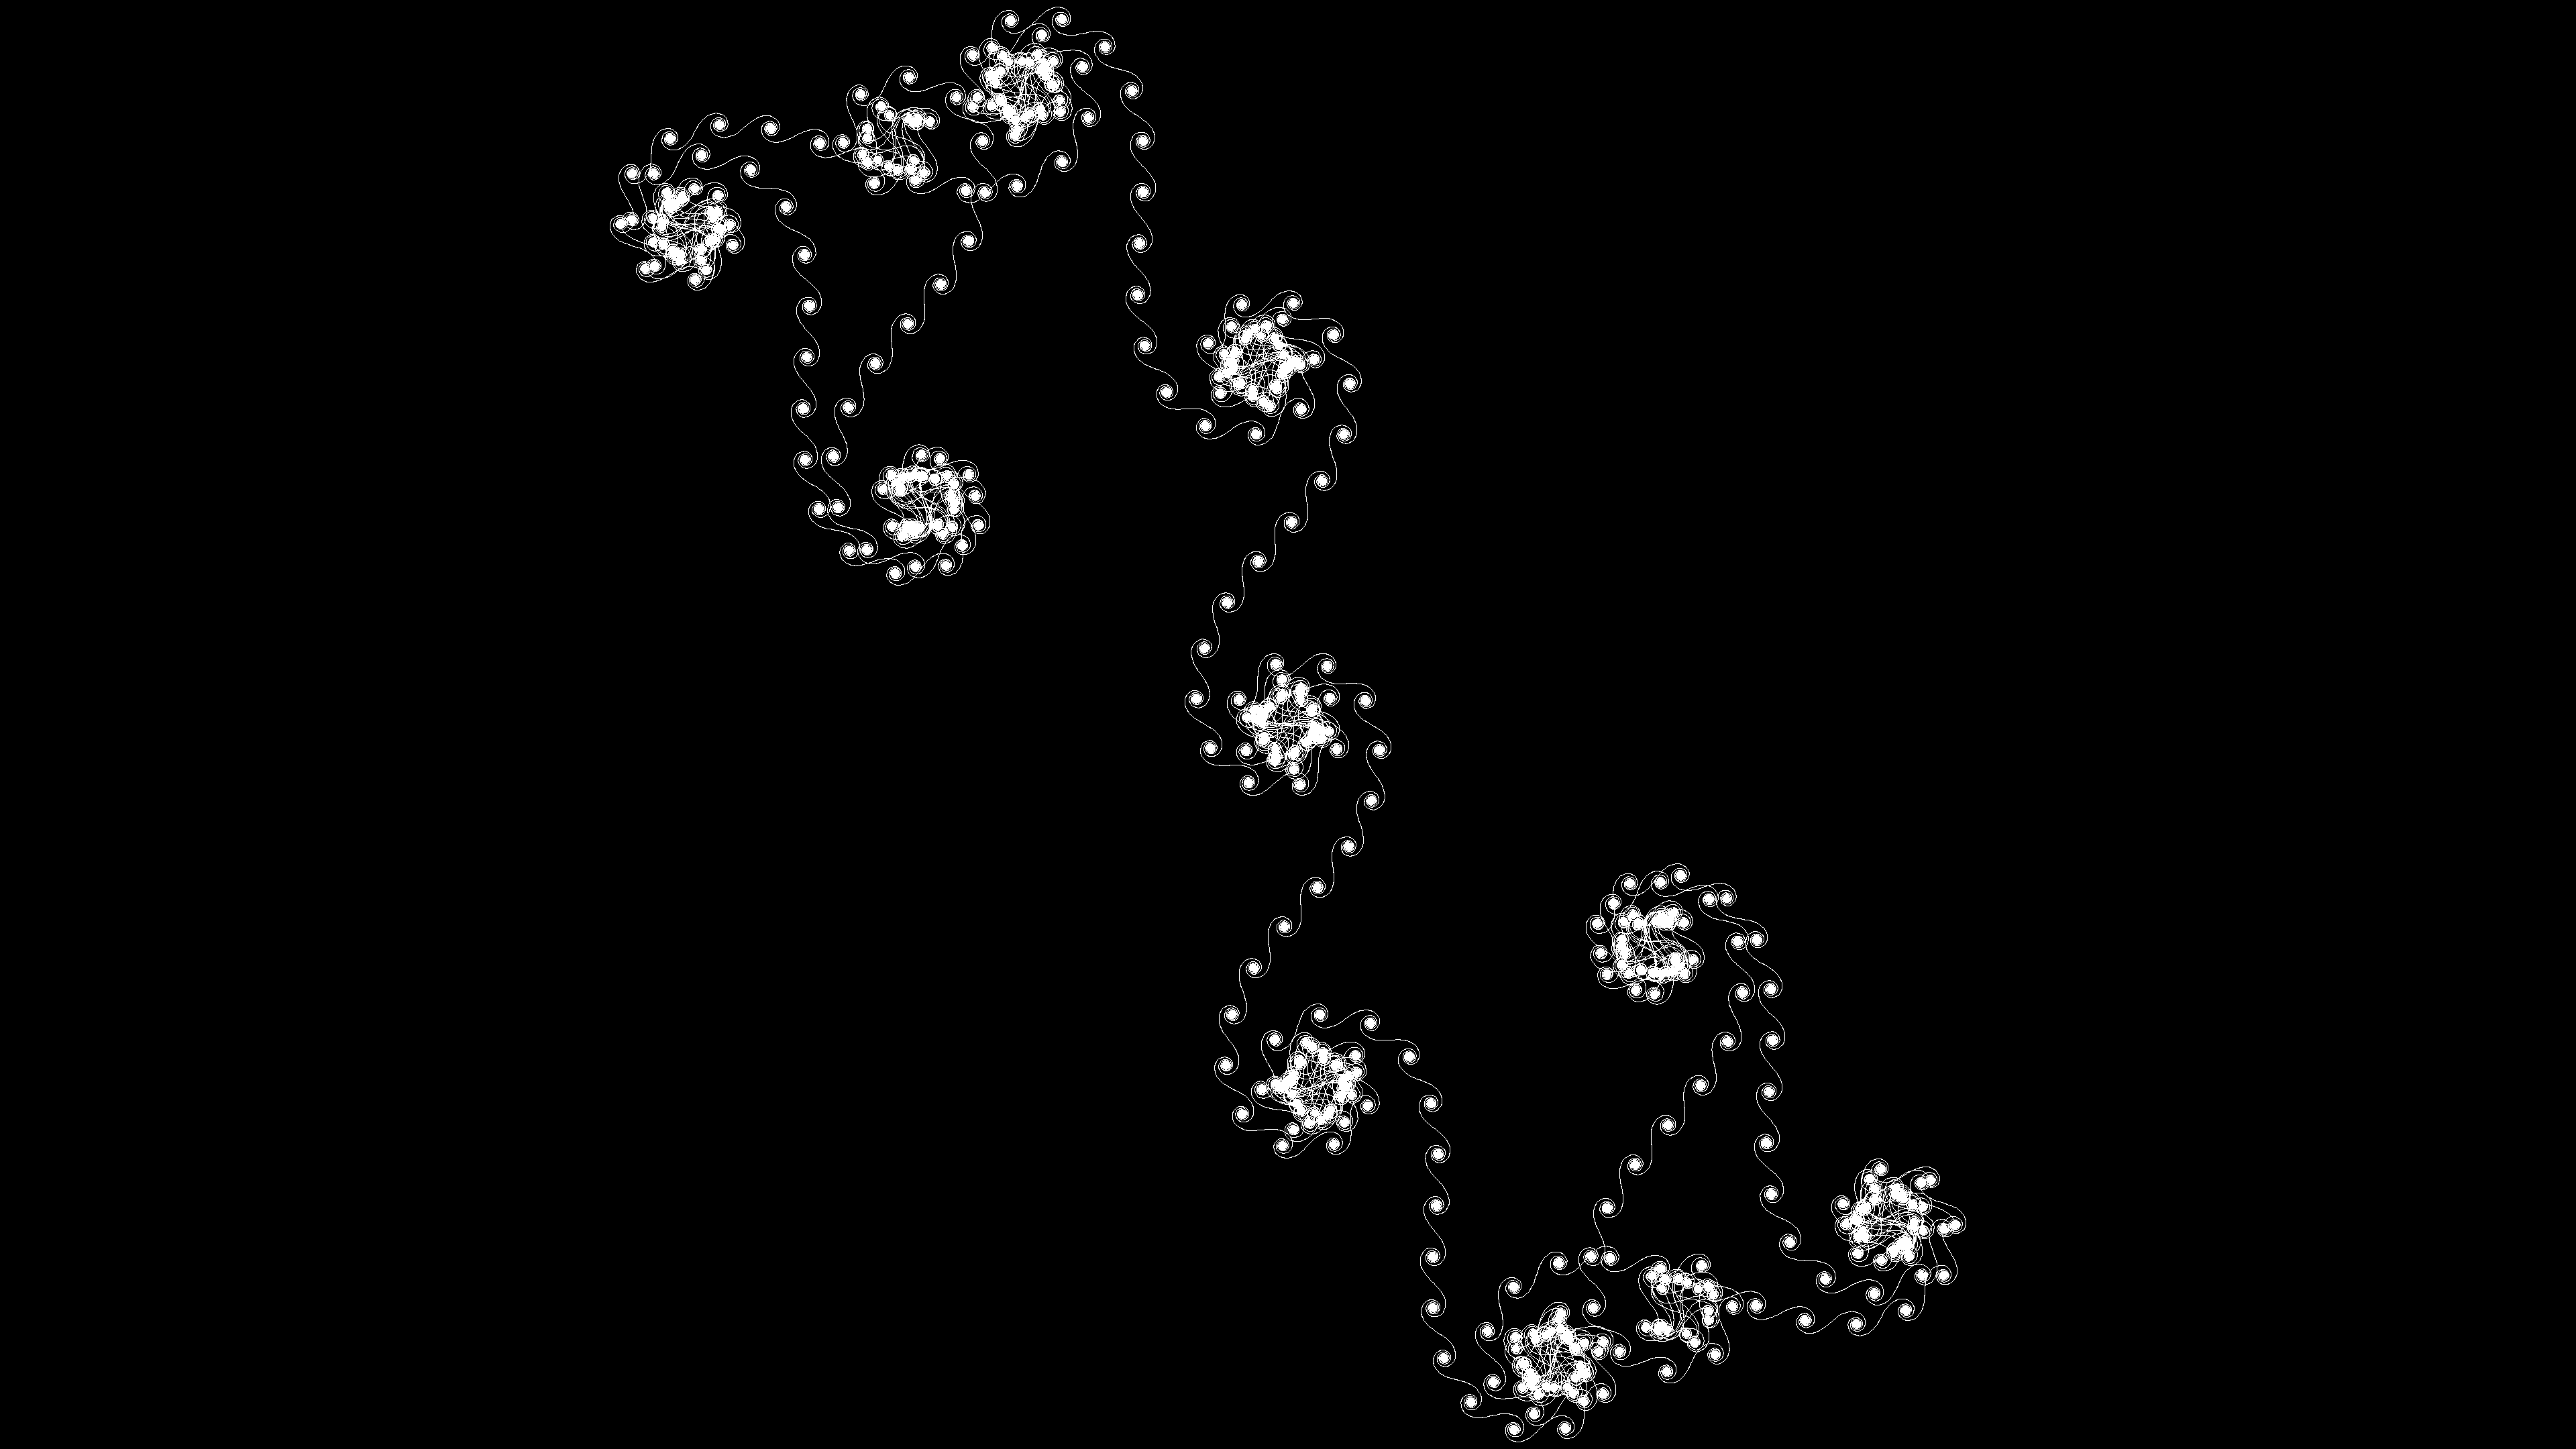
\includegraphics[width=\linewidth]{./stepsplusoneimages/0000000011.png}
    \caption{tf p=499 q=199610 theta=000 89995491.png}
  \end{subfigure}
  \begin{subfigure}[t]{0.48\textwidth}
    \centering
    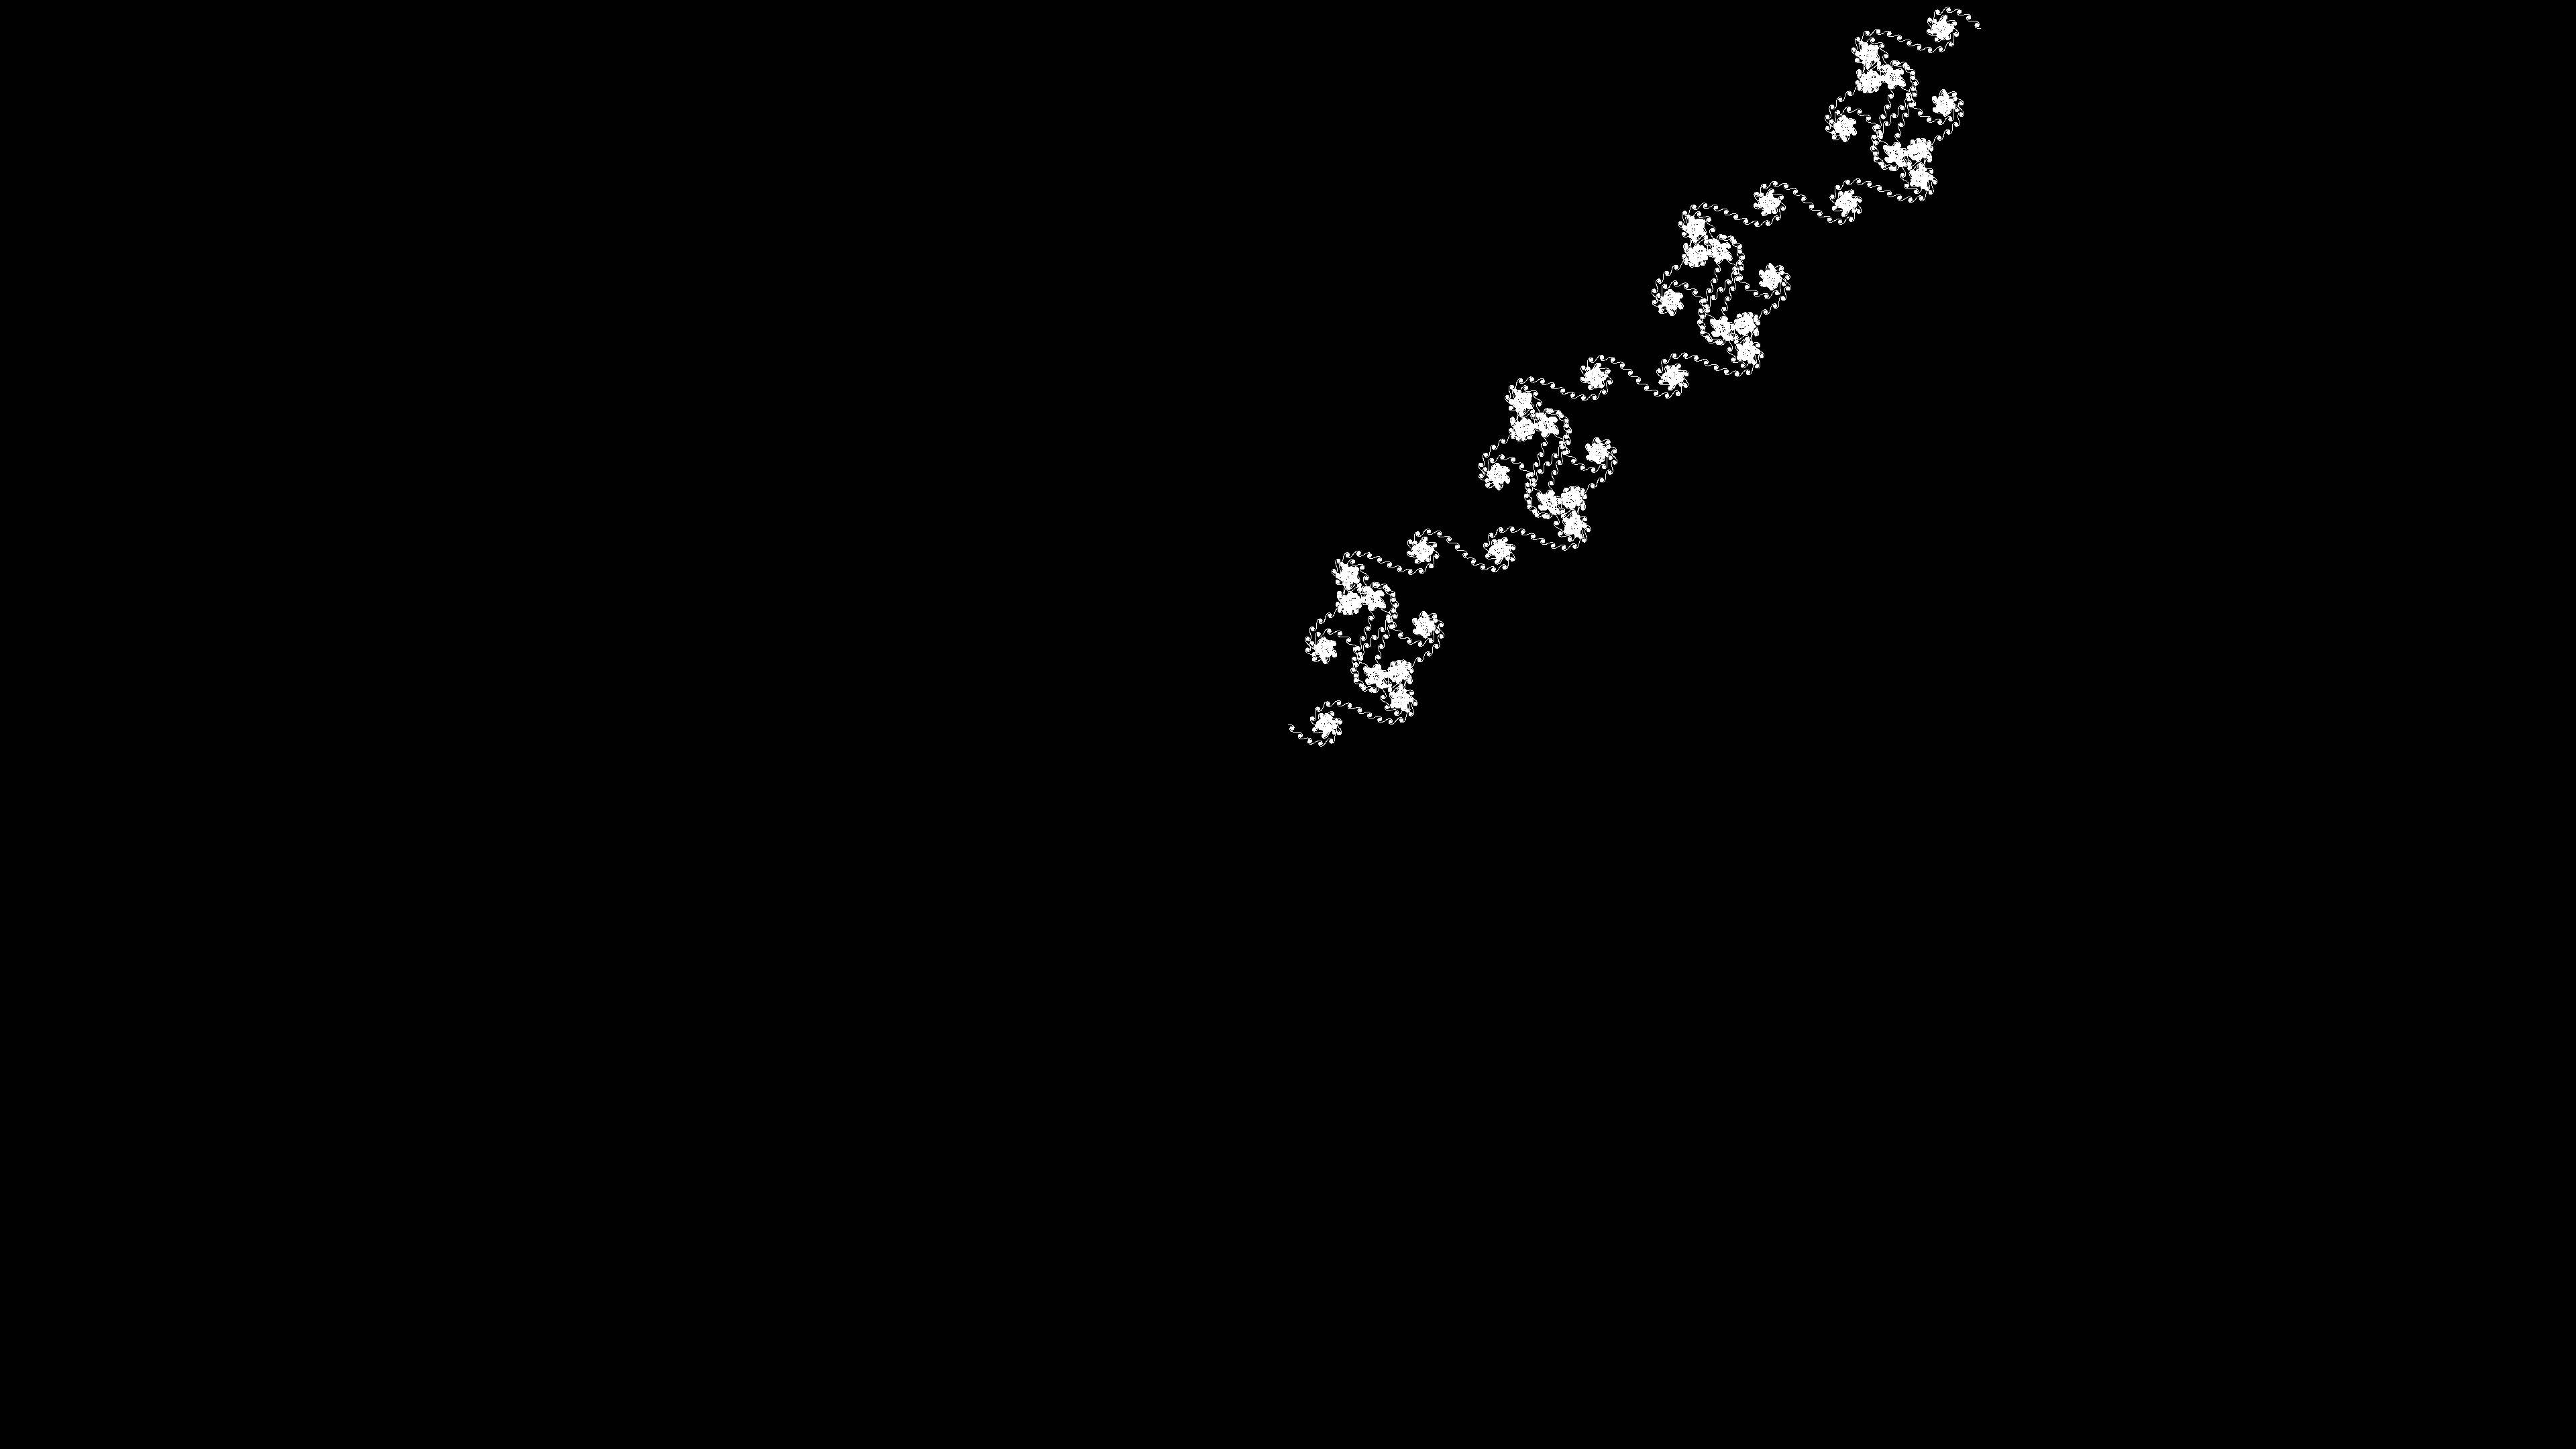
\includegraphics[width=\linewidth]{./stepsplusoneimages/0000000012.png}
    \caption{tf p=499 q=200109 theta=000 89771075.png}
  \end{subfigure}
  \caption{n=010 s=400 s+1=401}
  \label{fig:n=010}
\end{figure}
\begin{figure}[H]
  \centering
  \begin{subfigure}[t]{0.48\textwidth}
    \centering
    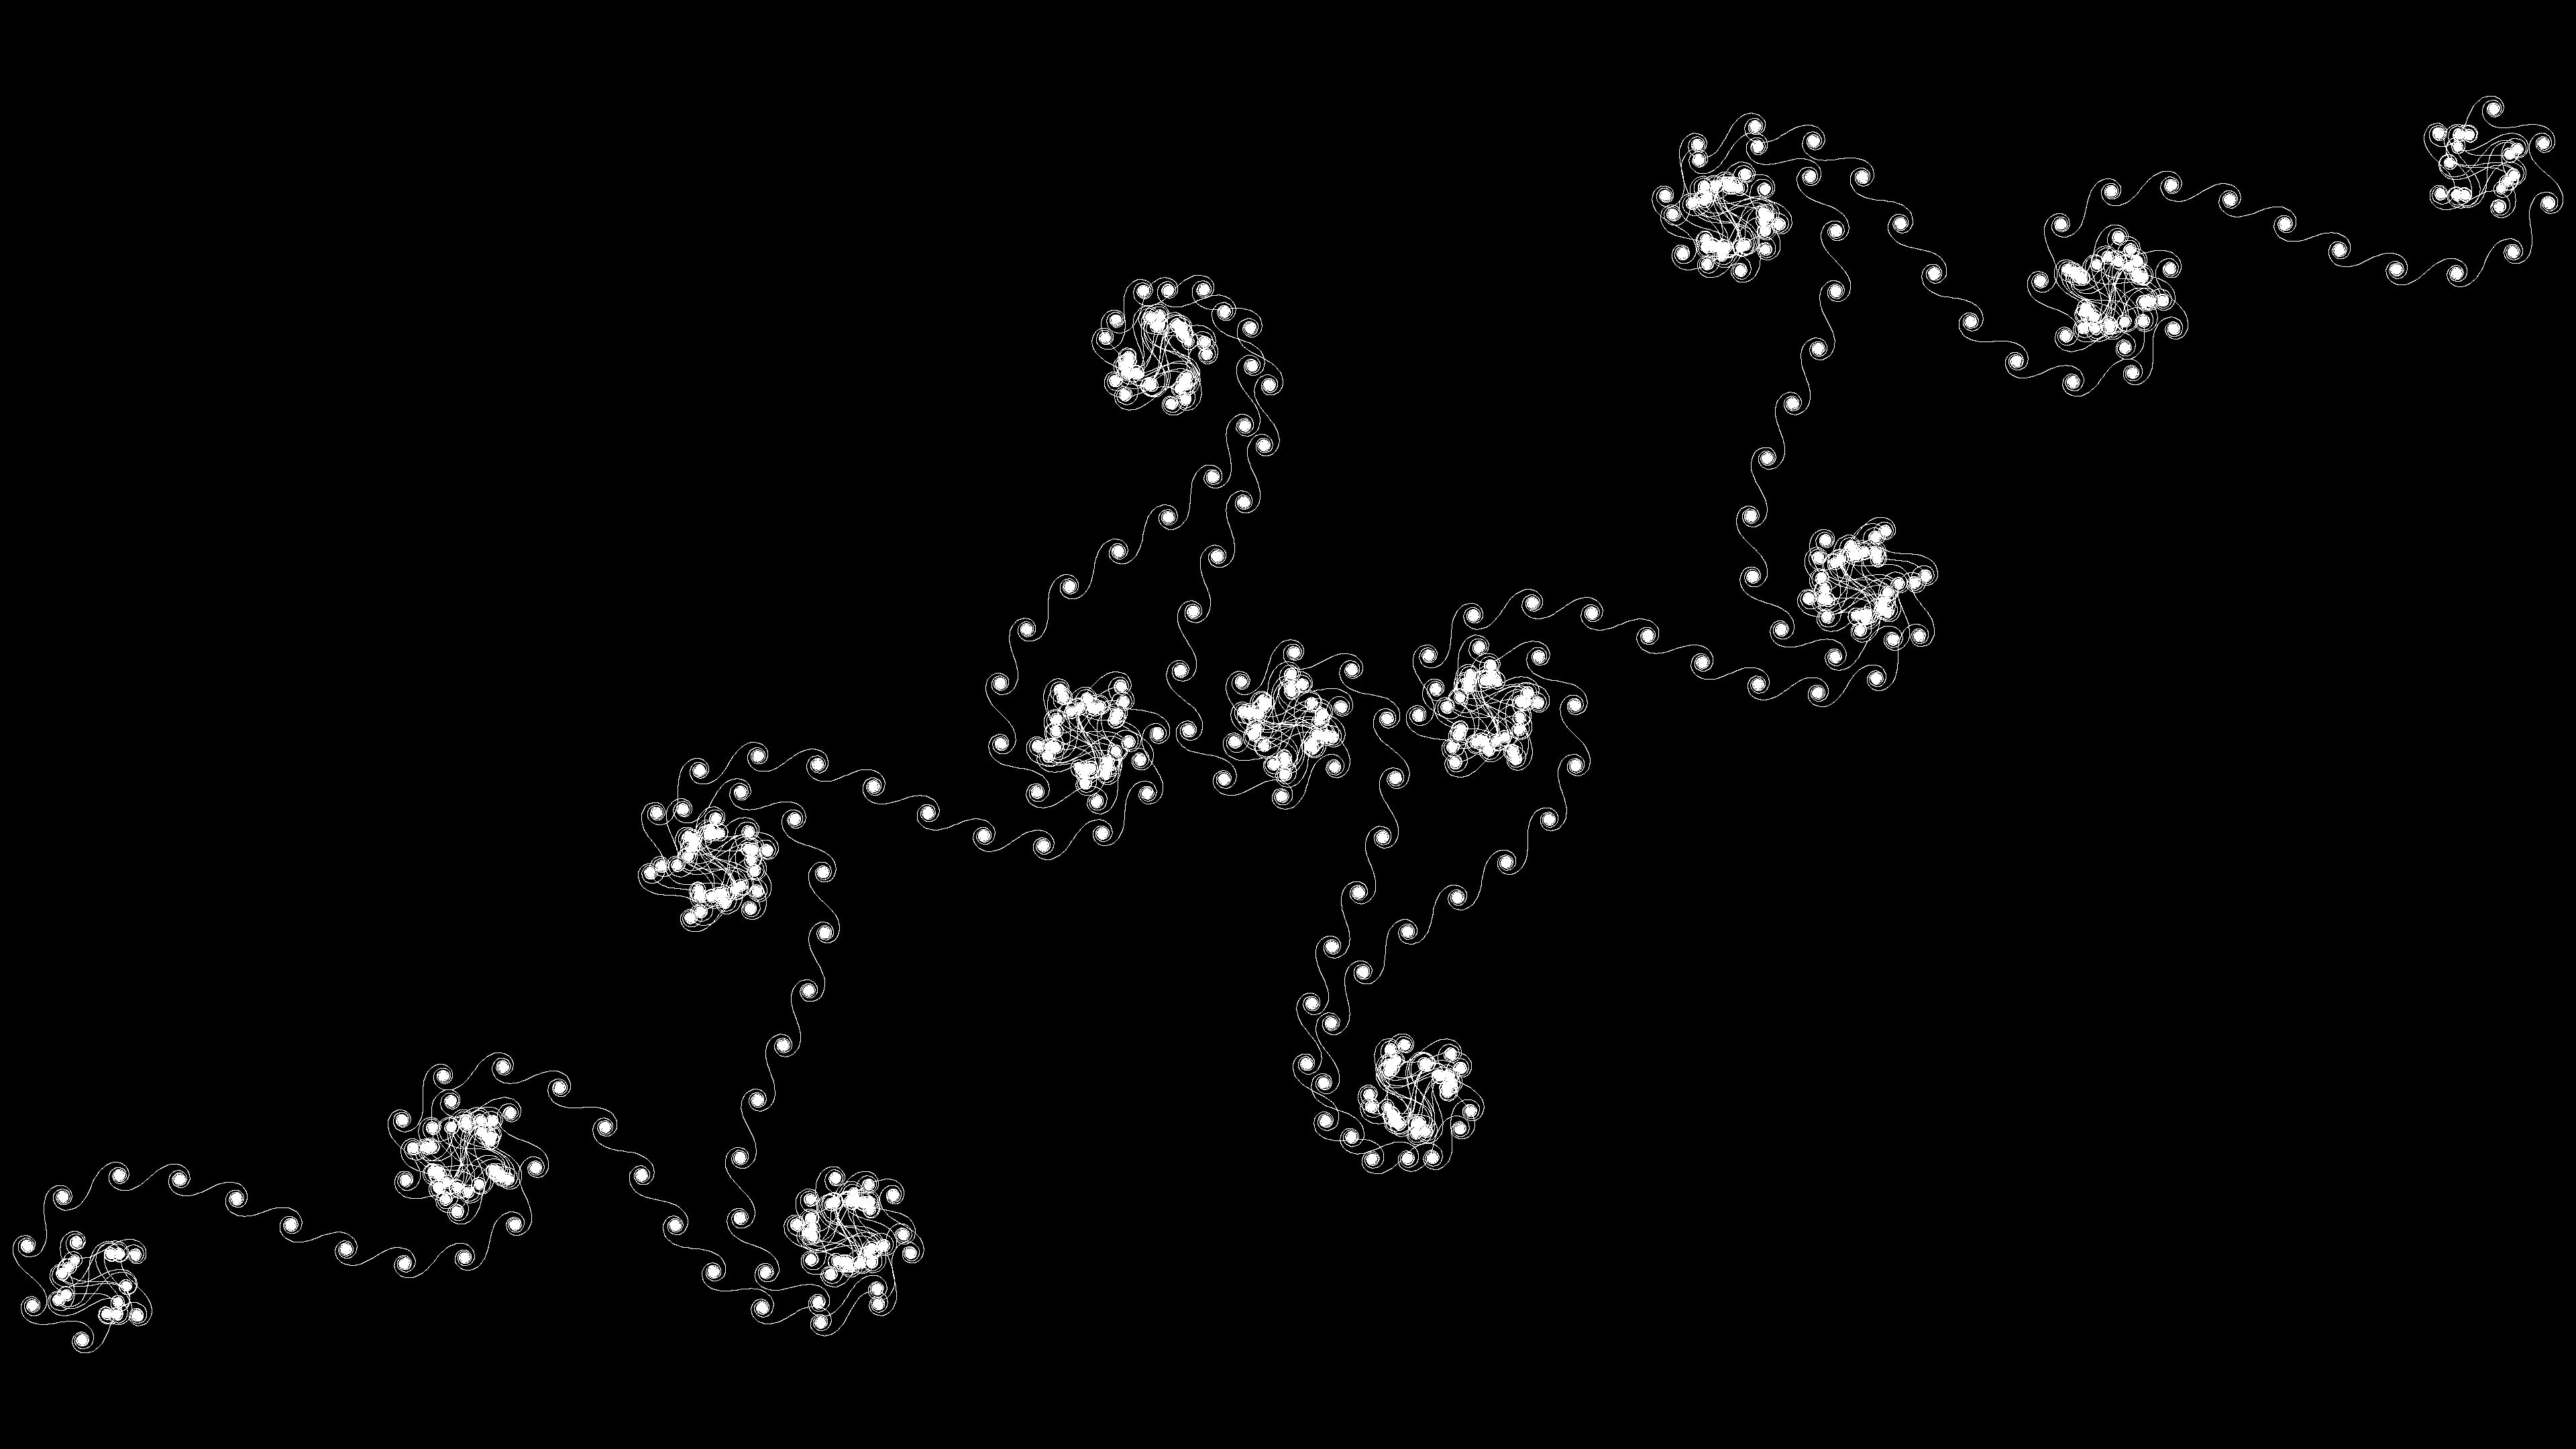
\includegraphics[width=\linewidth]{./stepsplusoneimages/0000000013.png}
    \caption{tf p=499 q=199612 theta=000 89994590.png}
  \end{subfigure}
  \begin{subfigure}[t]{0.48\textwidth}
    \centering
    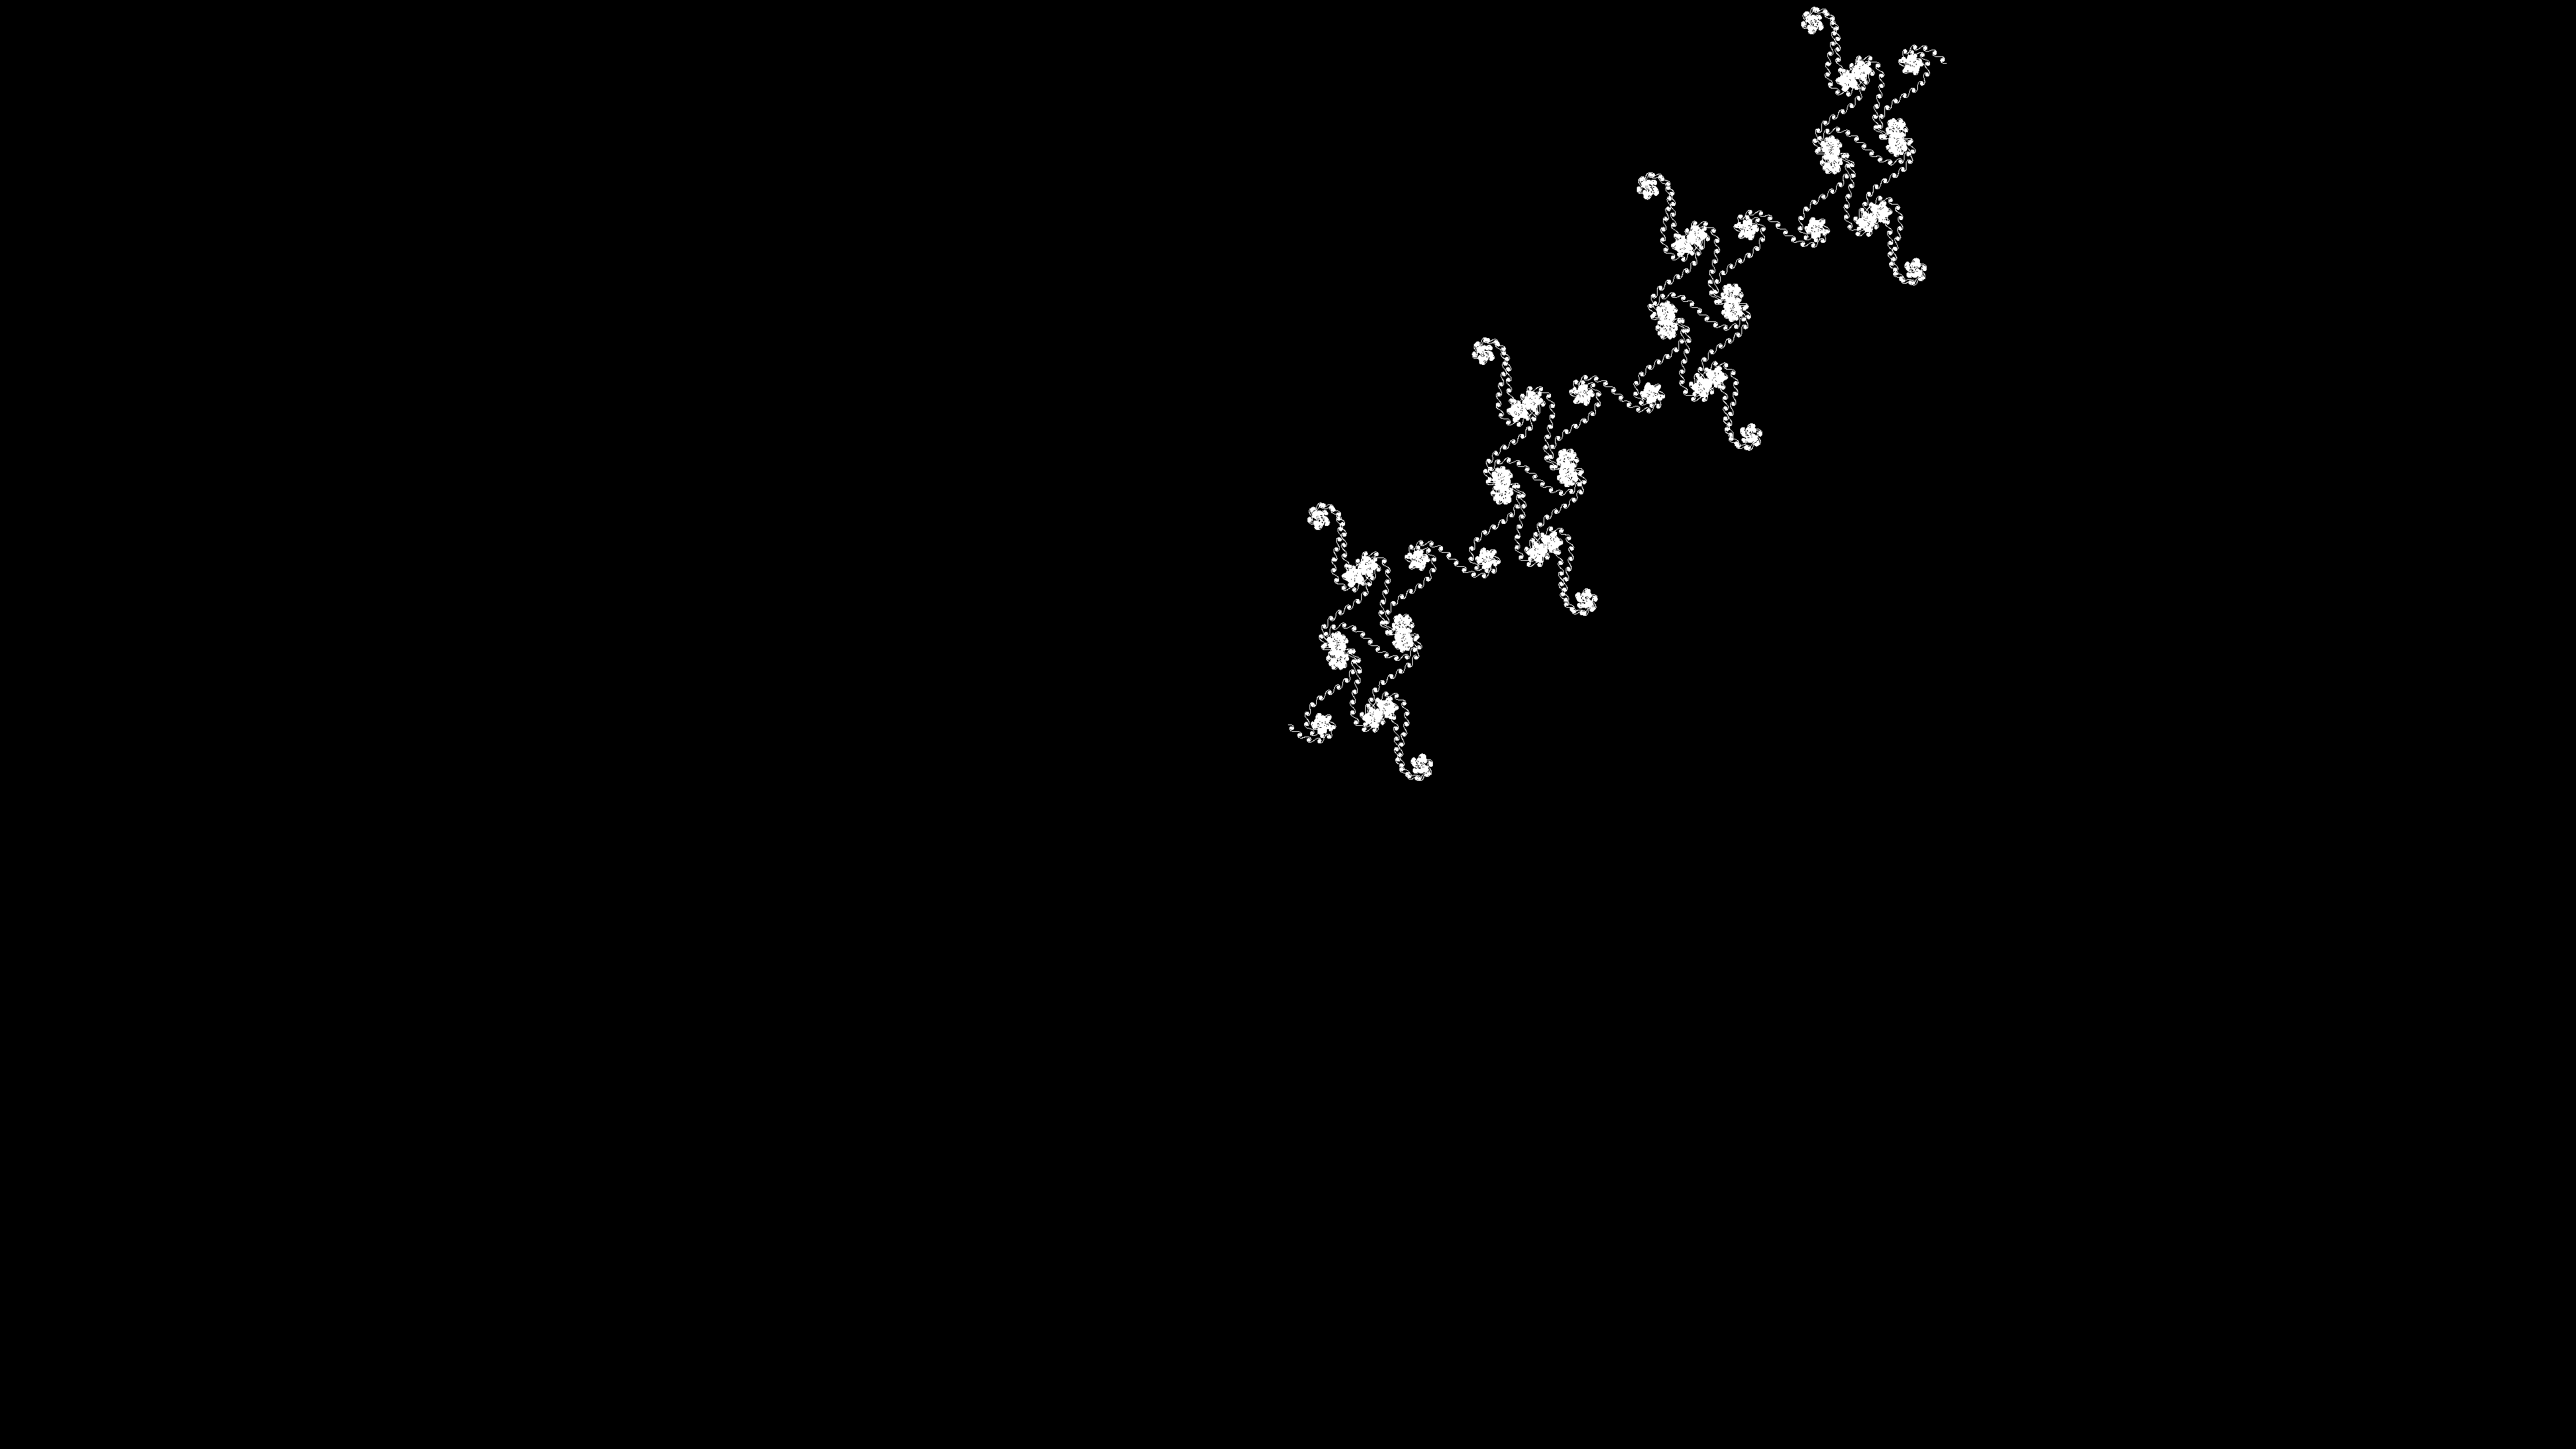
\includegraphics[width=\linewidth]{./stepsplusoneimages/0000000014.png}
    \caption{tf p=499 q=200111 theta=000 89770178.png}
  \end{subfigure}
  \caption{n=012 s=400 s+1=401}
  \label{fig:n=012}
\end{figure}
\begin{figure}[H]
  \centering
  \begin{subfigure}[t]{0.48\textwidth}
    \centering
    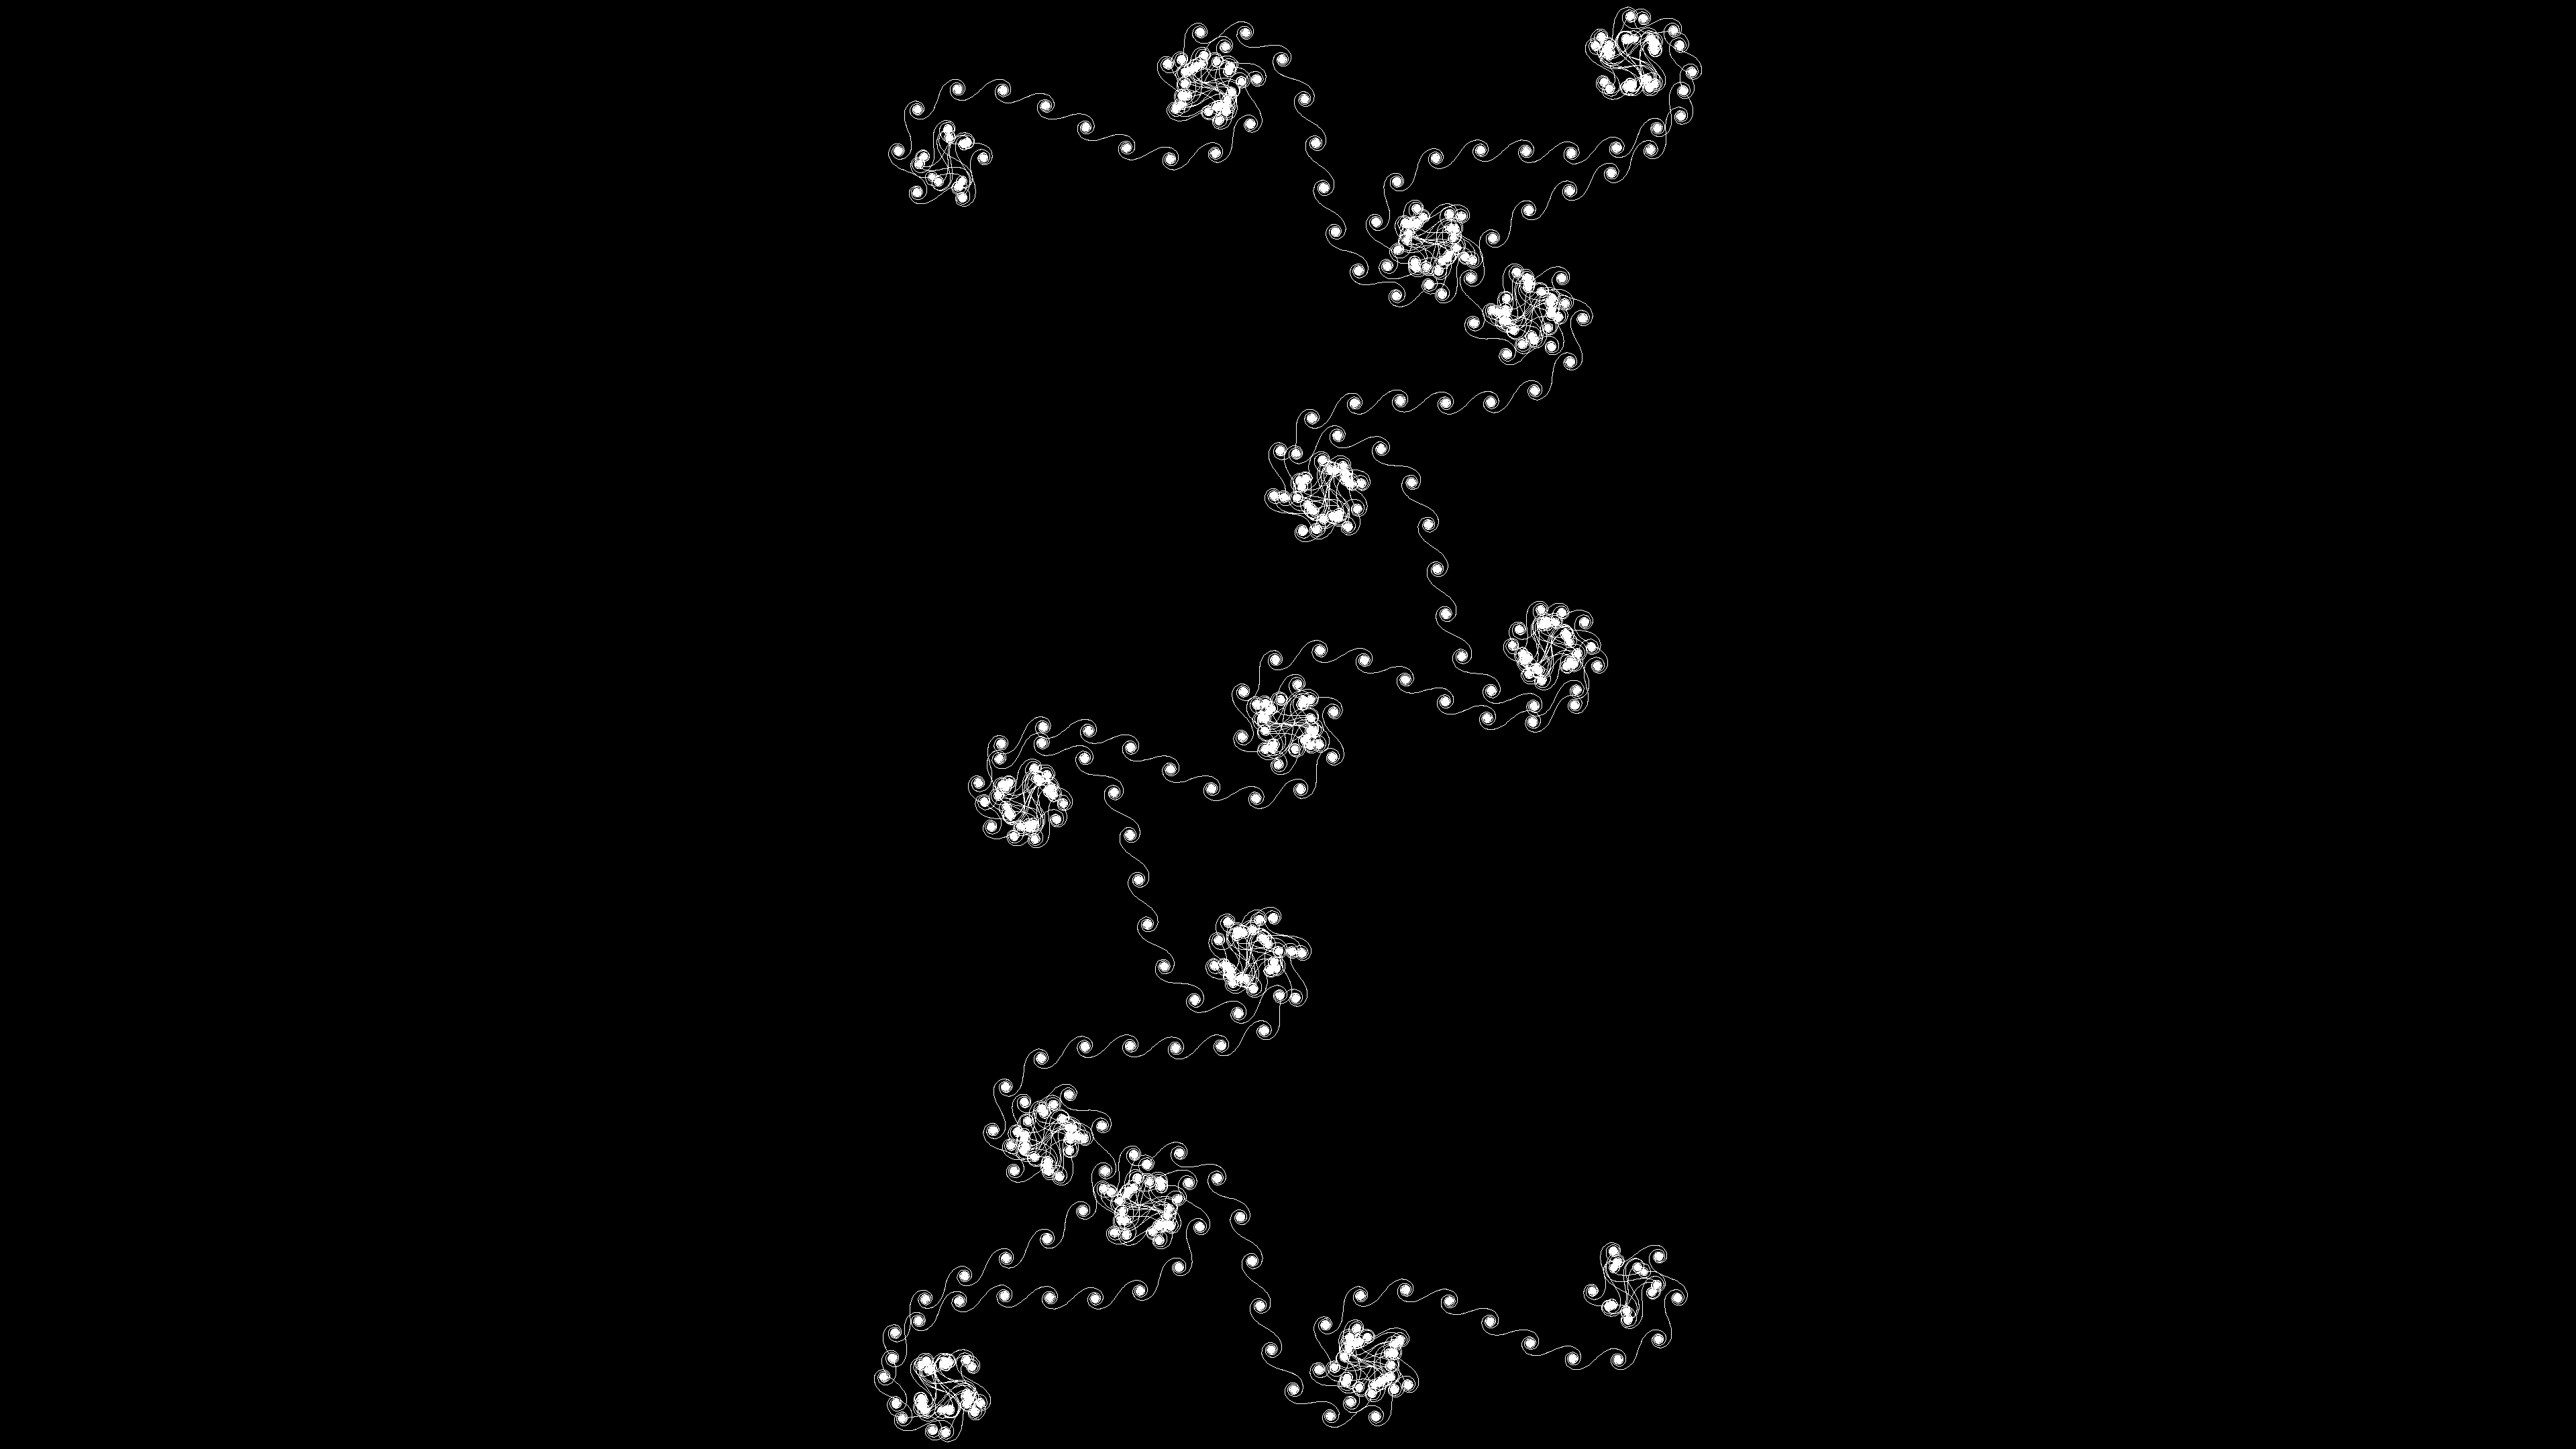
\includegraphics[width=\linewidth]{./stepsplusoneimages/0000000015.png}
    \caption{tf p=499 q=199614 theta=000 89993688.png}
  \end{subfigure}
  \begin{subfigure}[t]{0.48\textwidth}
    \centering
    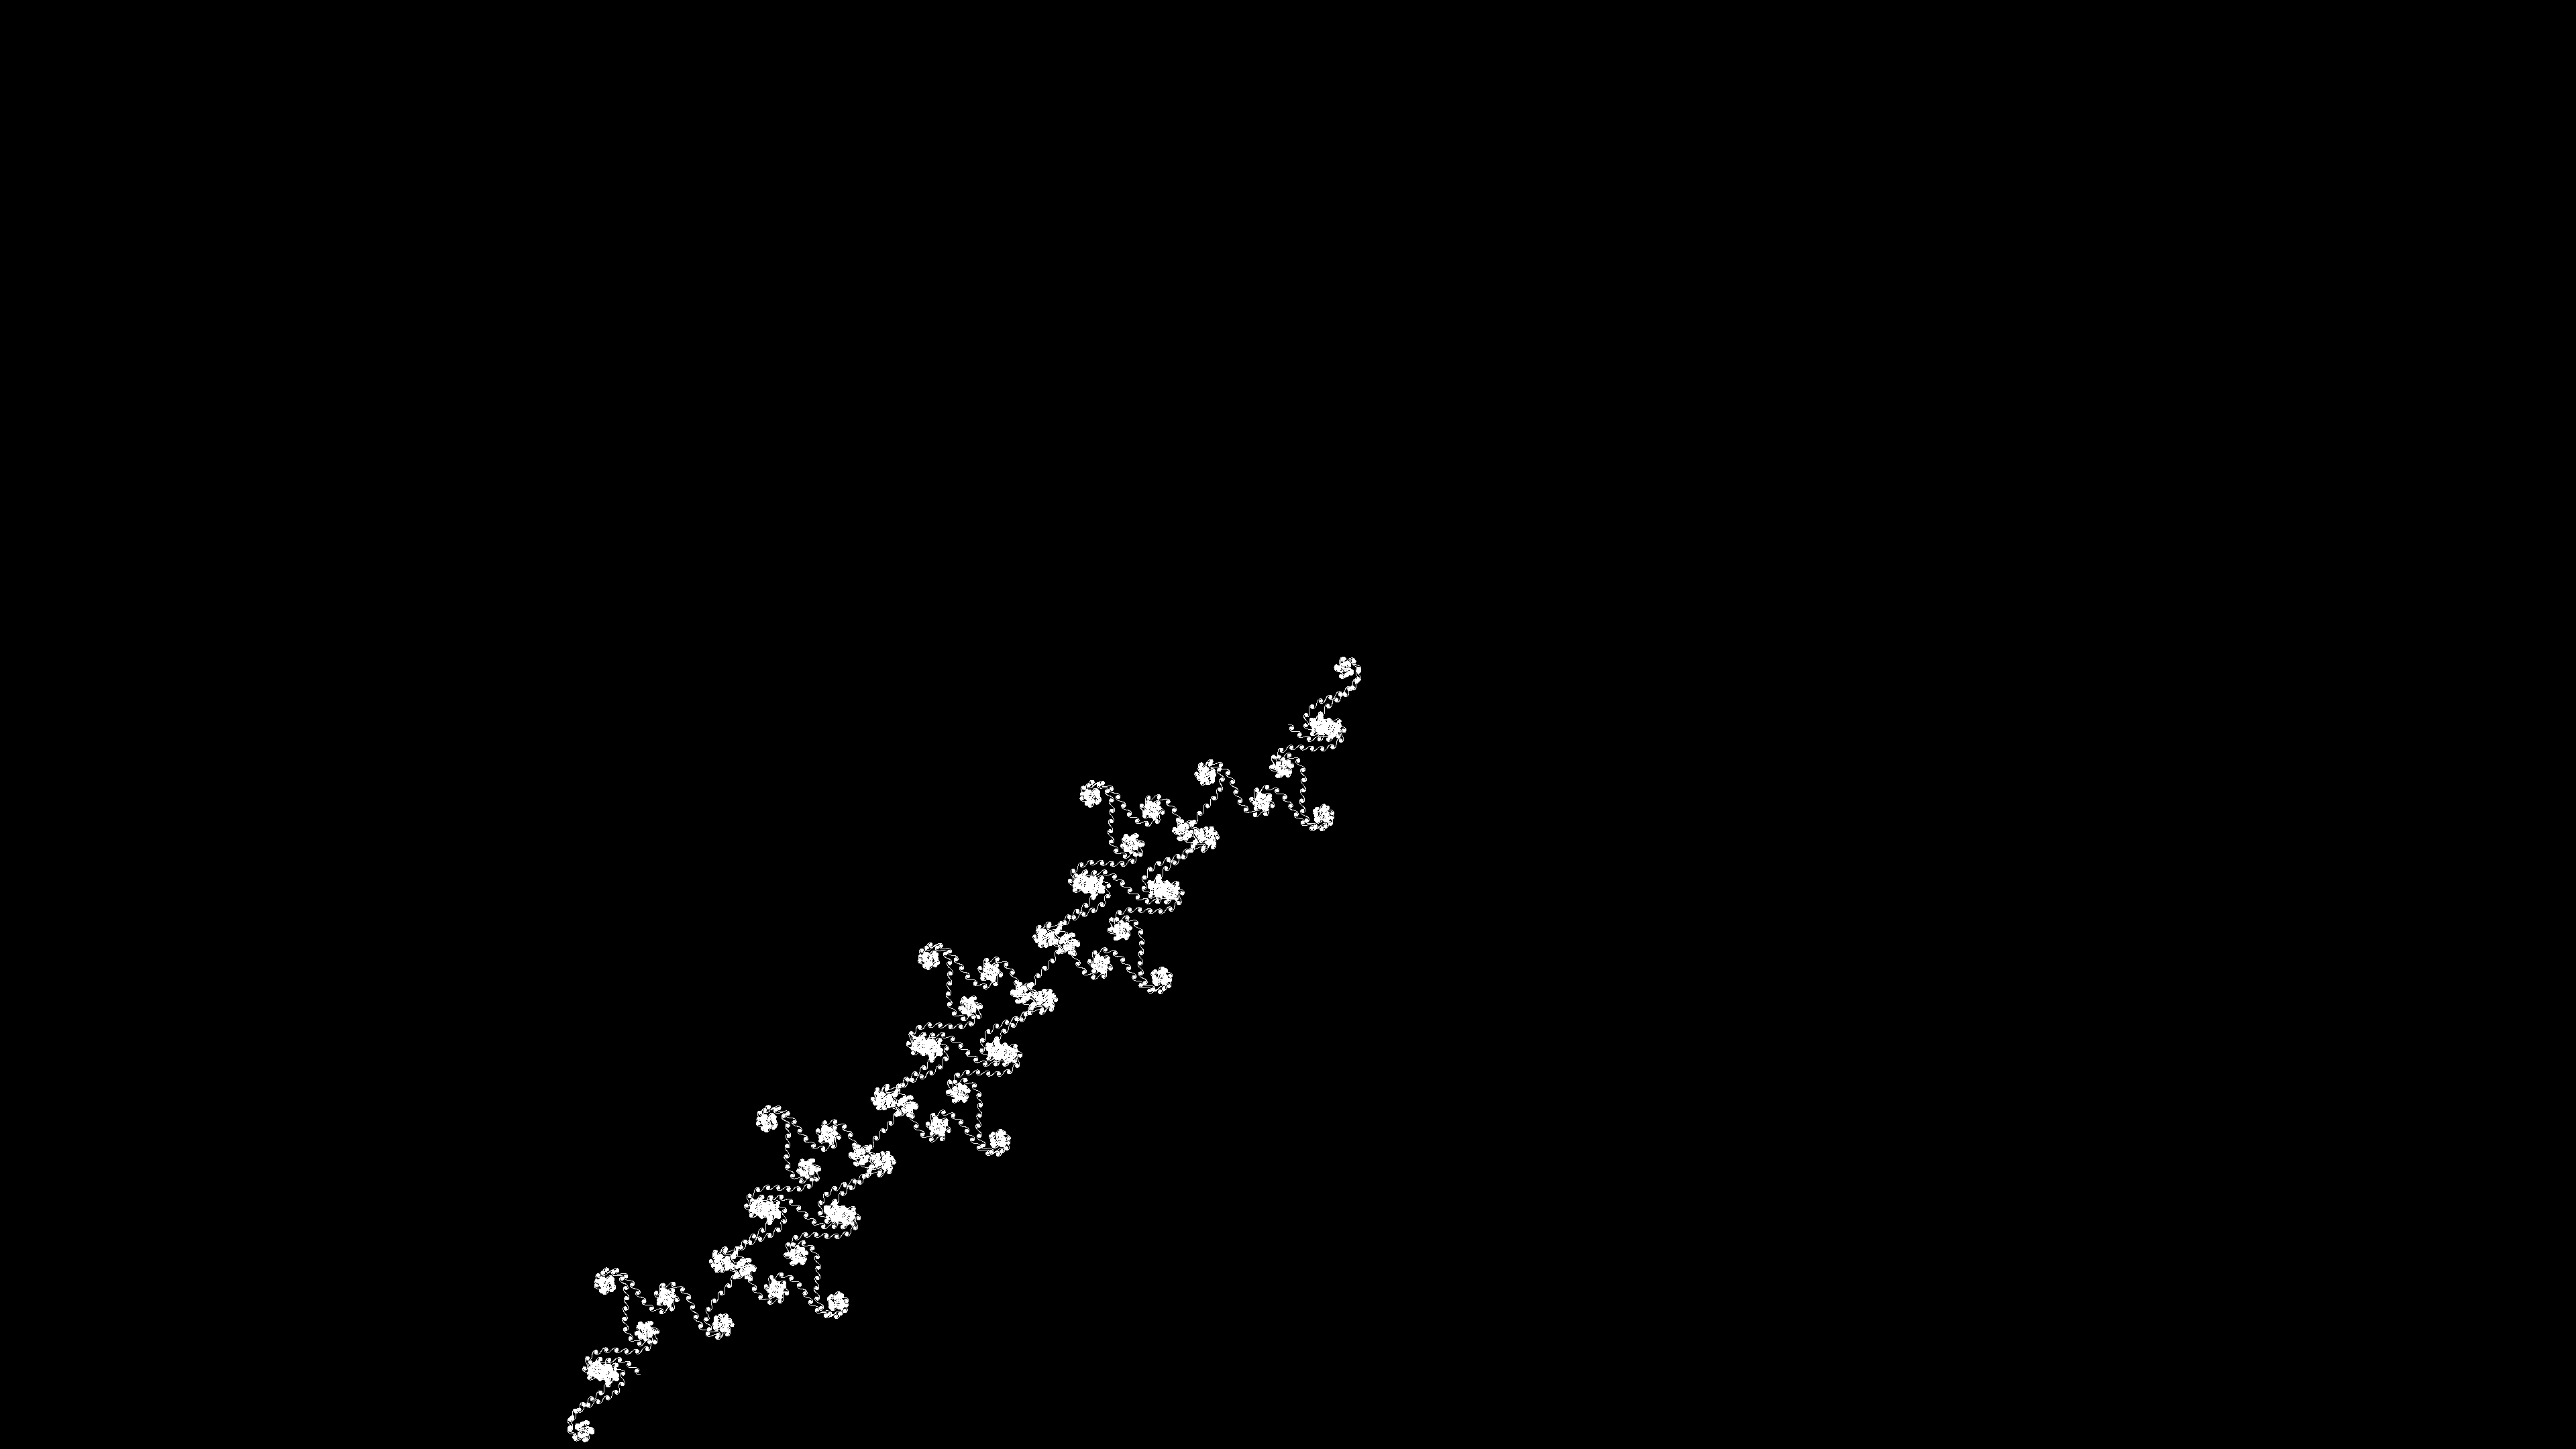
\includegraphics[width=\linewidth]{./stepsplusoneimages/0000000016.png}
    \caption{tf p=499 q=200113 theta=000 89769280.png}
  \end{subfigure}
  \caption{n=014 s=400 s+1=401}
  \label{fig:n=014}
\end{figure}
\begin{figure}[H]
  \centering
  \begin{subfigure}[t]{0.48\textwidth}
    \centering
    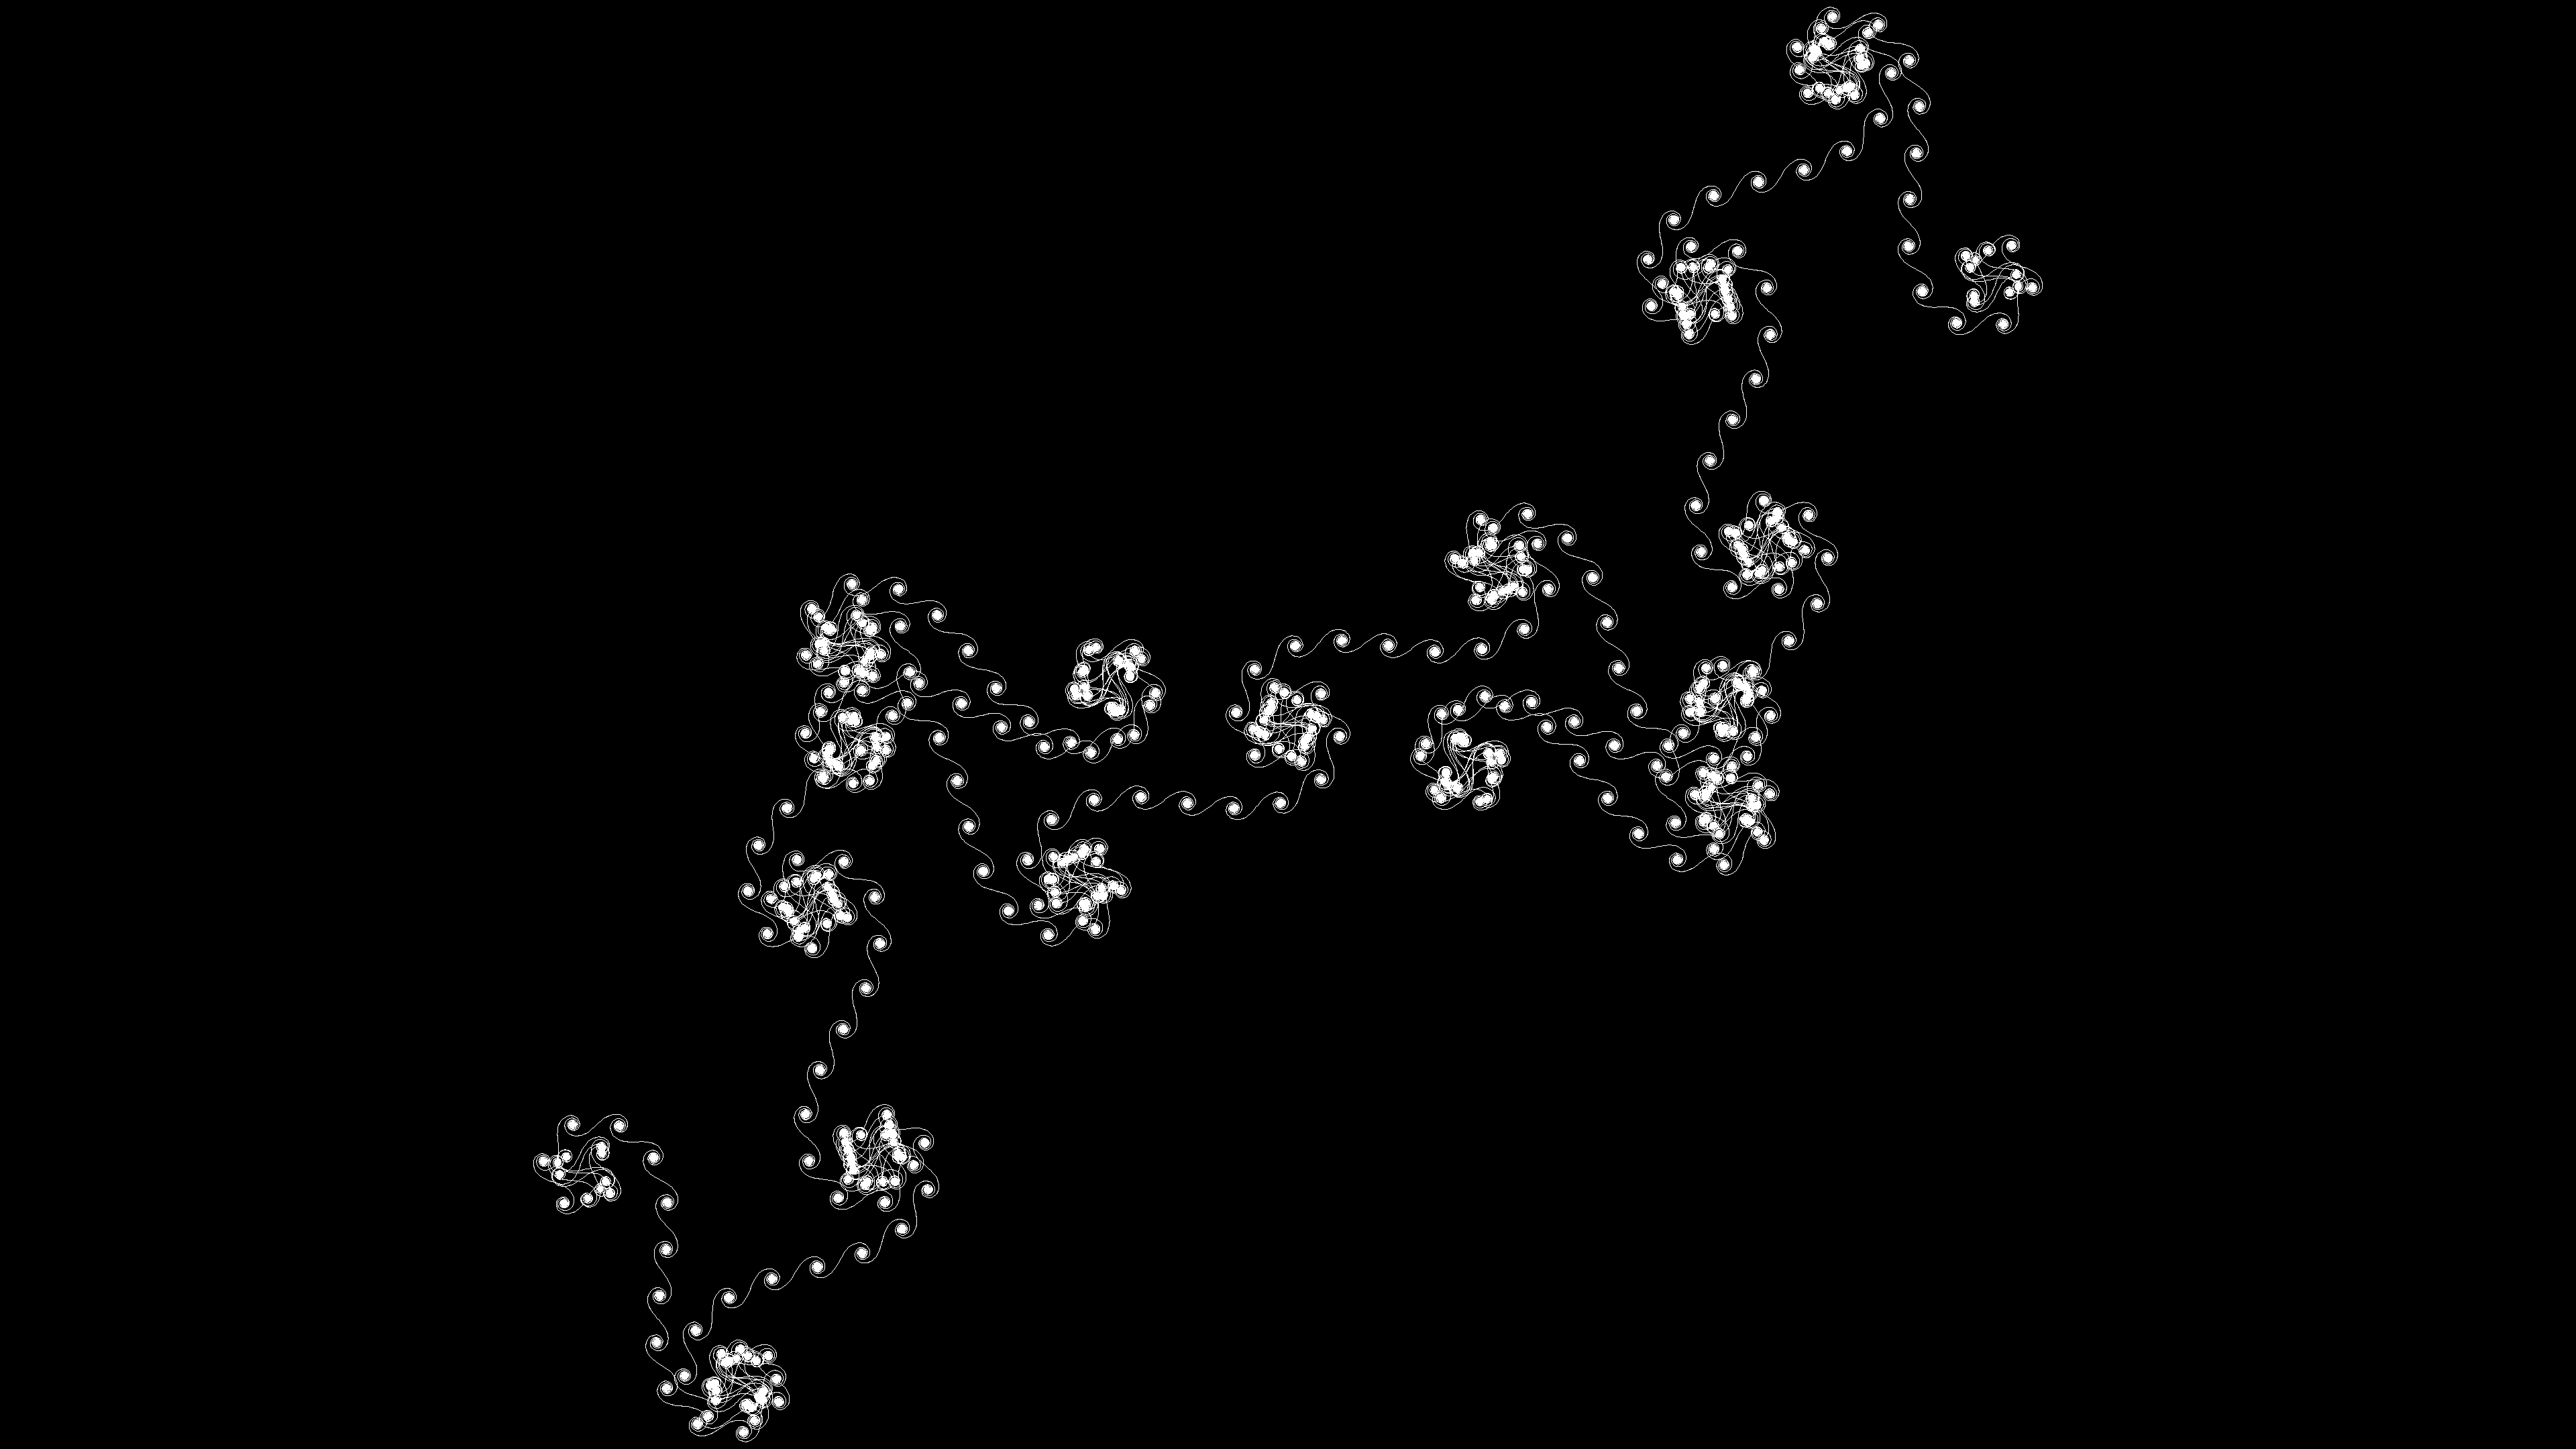
\includegraphics[width=\linewidth]{./stepsplusoneimages/0000000017.png}
    \caption{tf p=499 q=199616 theta=000 89992786.png}
  \end{subfigure}
  \begin{subfigure}[t]{0.48\textwidth}
    \centering
    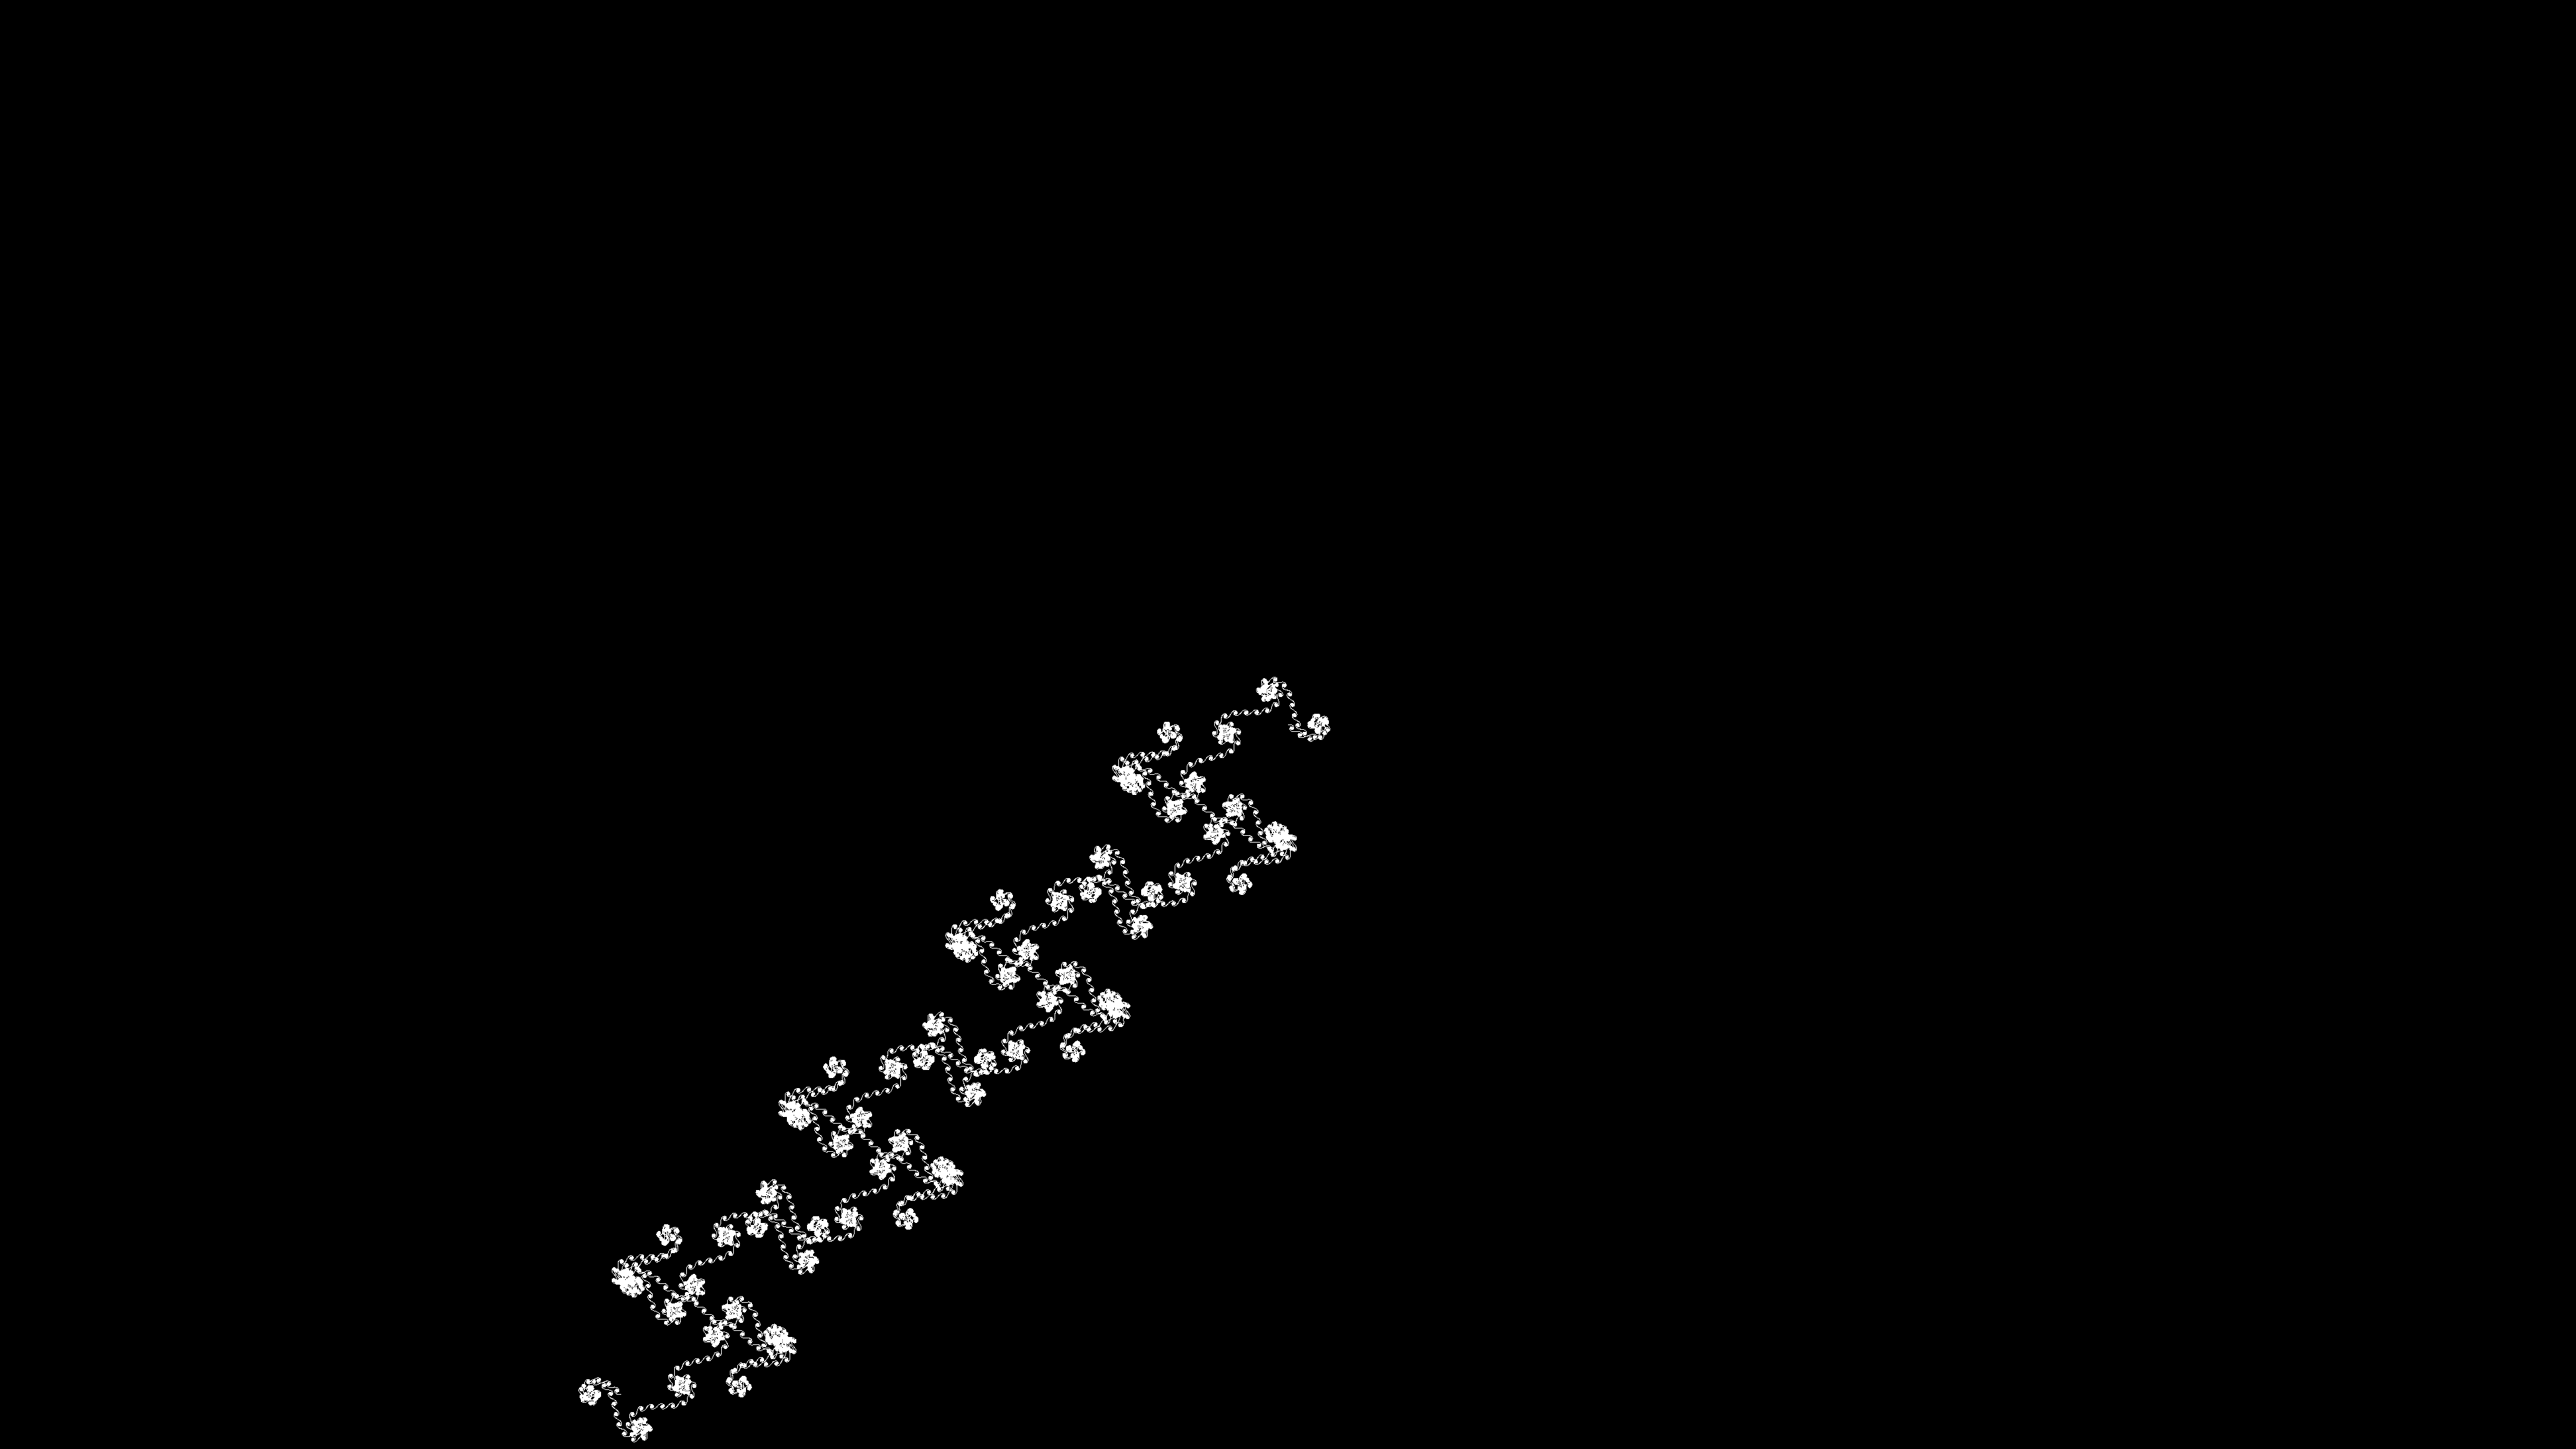
\includegraphics[width=\linewidth]{./stepsplusoneimages/0000000018.png}
    \caption{tf p=499 q=200115 theta=000 89768383.png}
  \end{subfigure}
  \caption{n=016 s=400 s+1=401}
  \label{fig:n=016}
\end{figure}
\begin{figure}[H]
  \centering
  \begin{subfigure}[t]{0.48\textwidth}
    \centering
    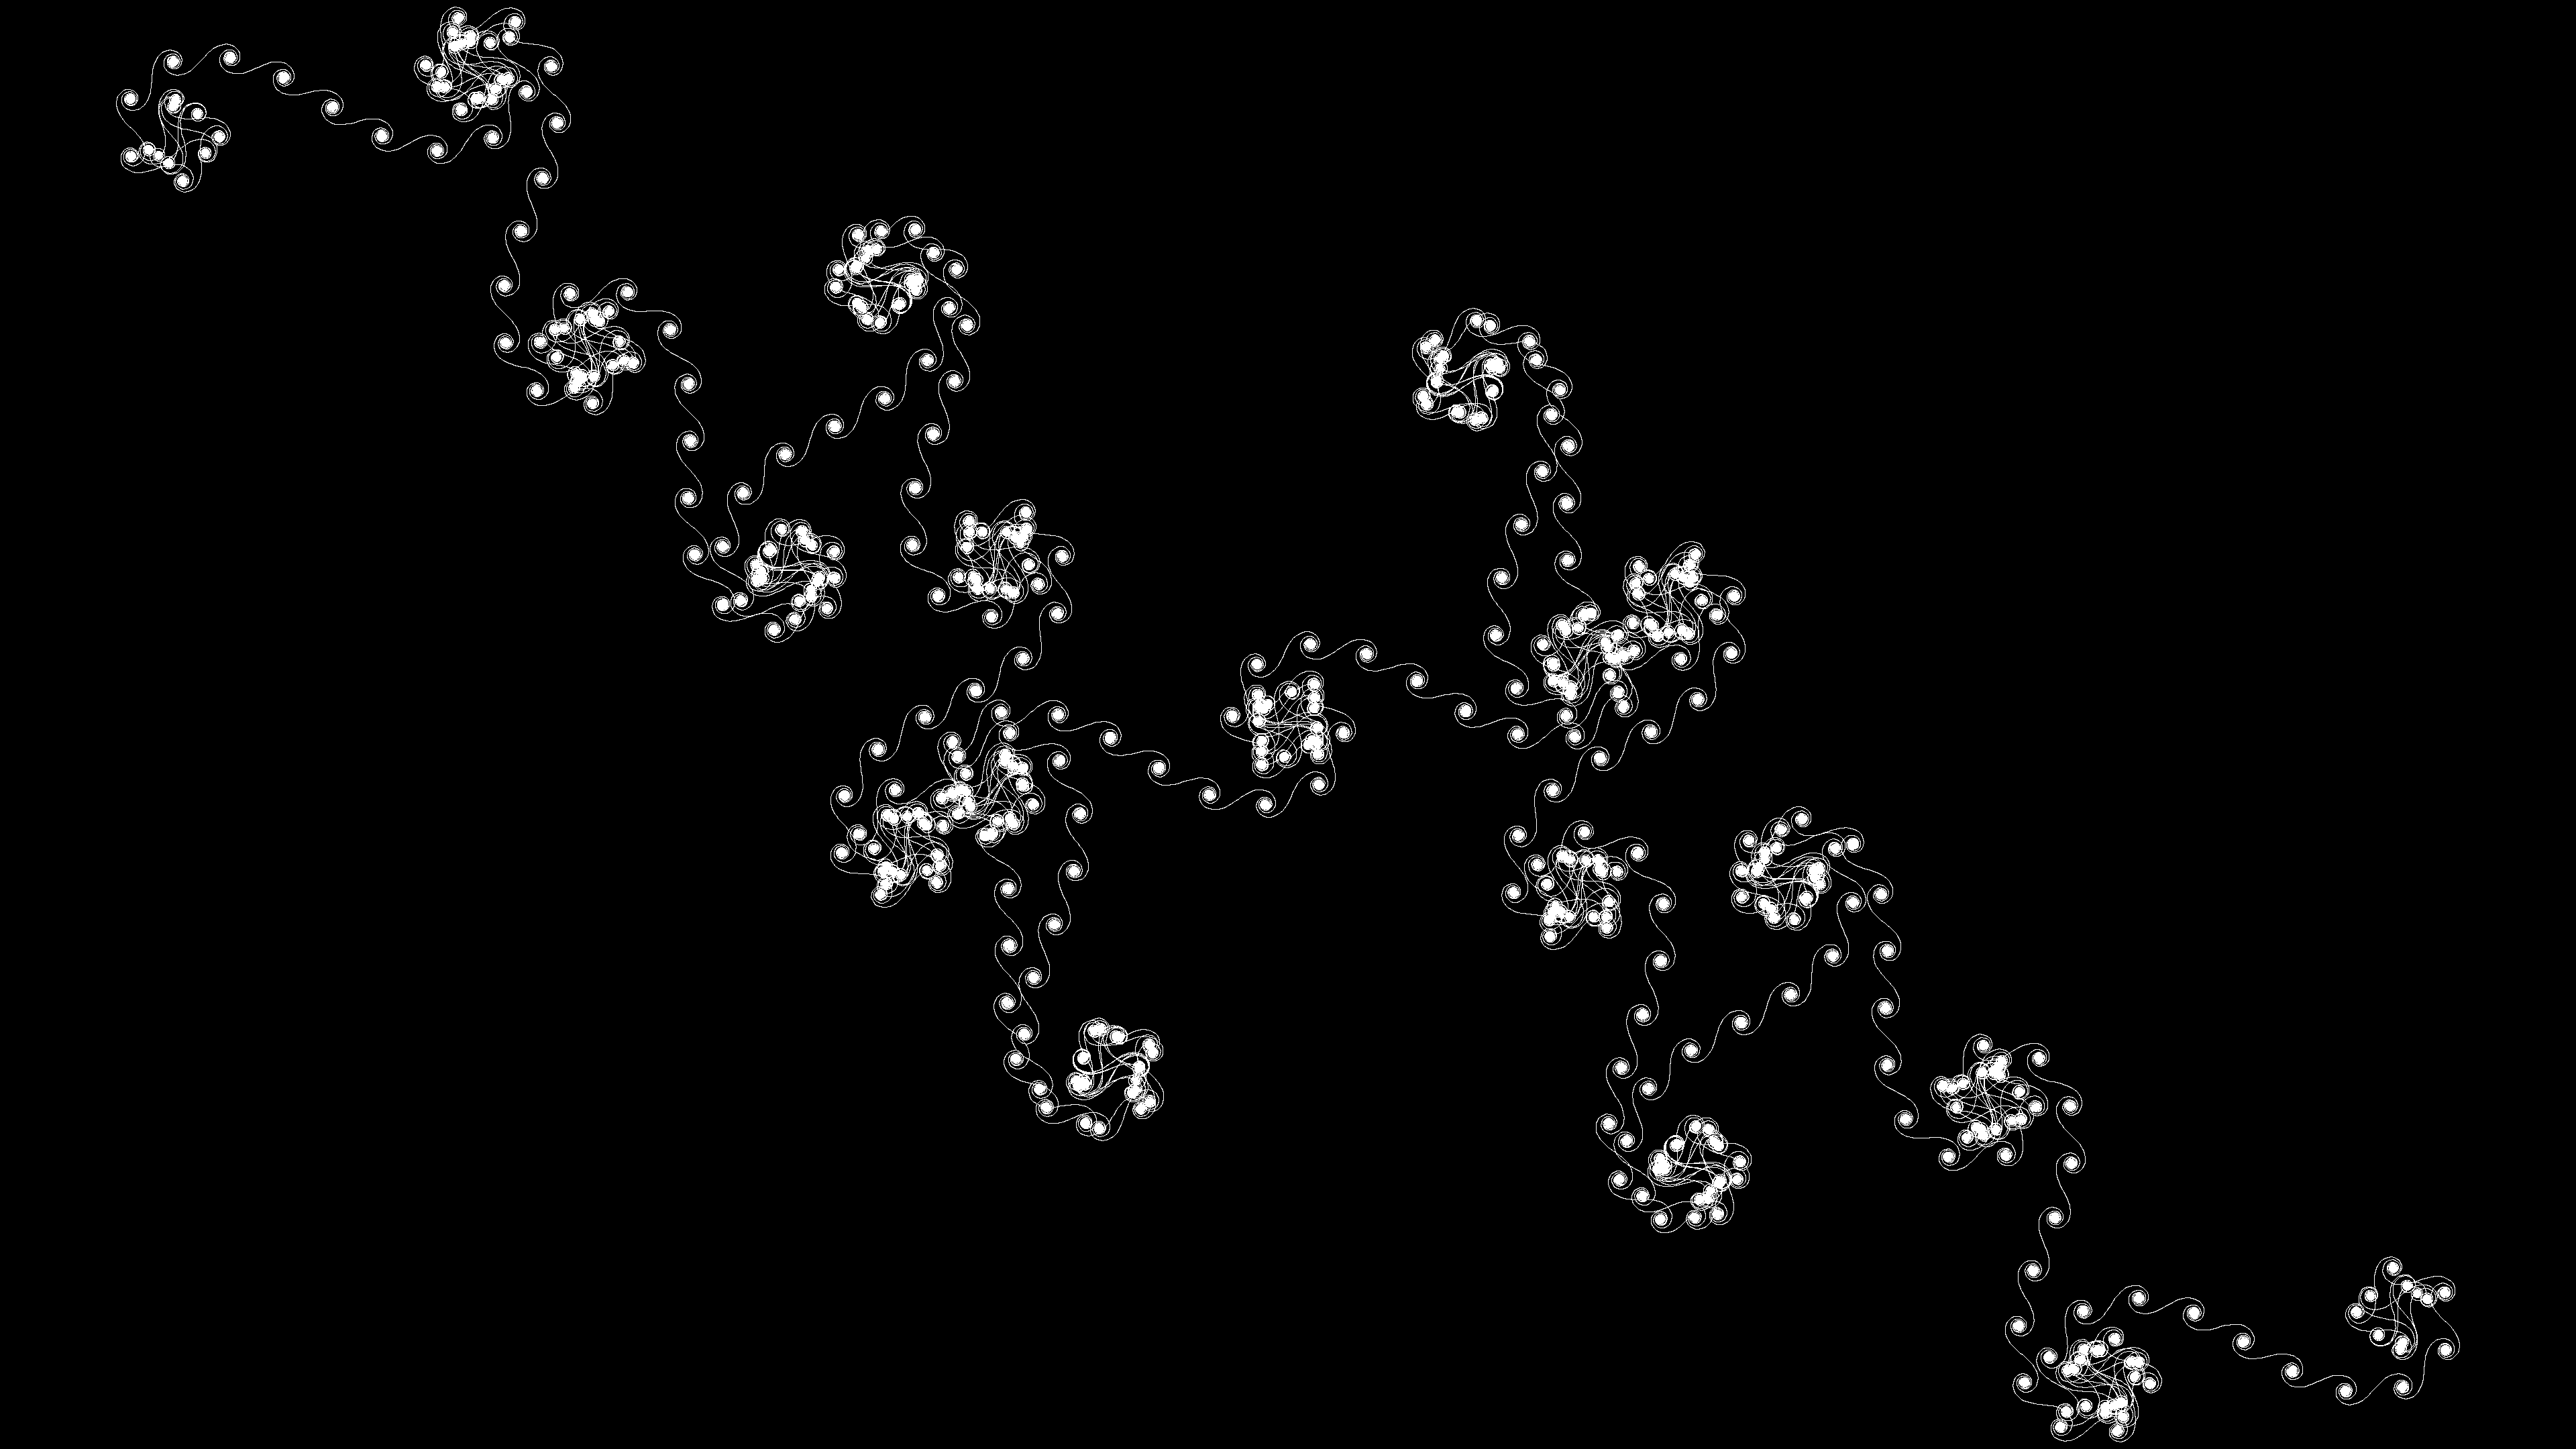
\includegraphics[width=\linewidth]{./stepsplusoneimages/0000000019.png}
    \caption{tf p=499 q=199618 theta=000 89991884.png}
  \end{subfigure}
  \begin{subfigure}[t]{0.48\textwidth}
    \centering
    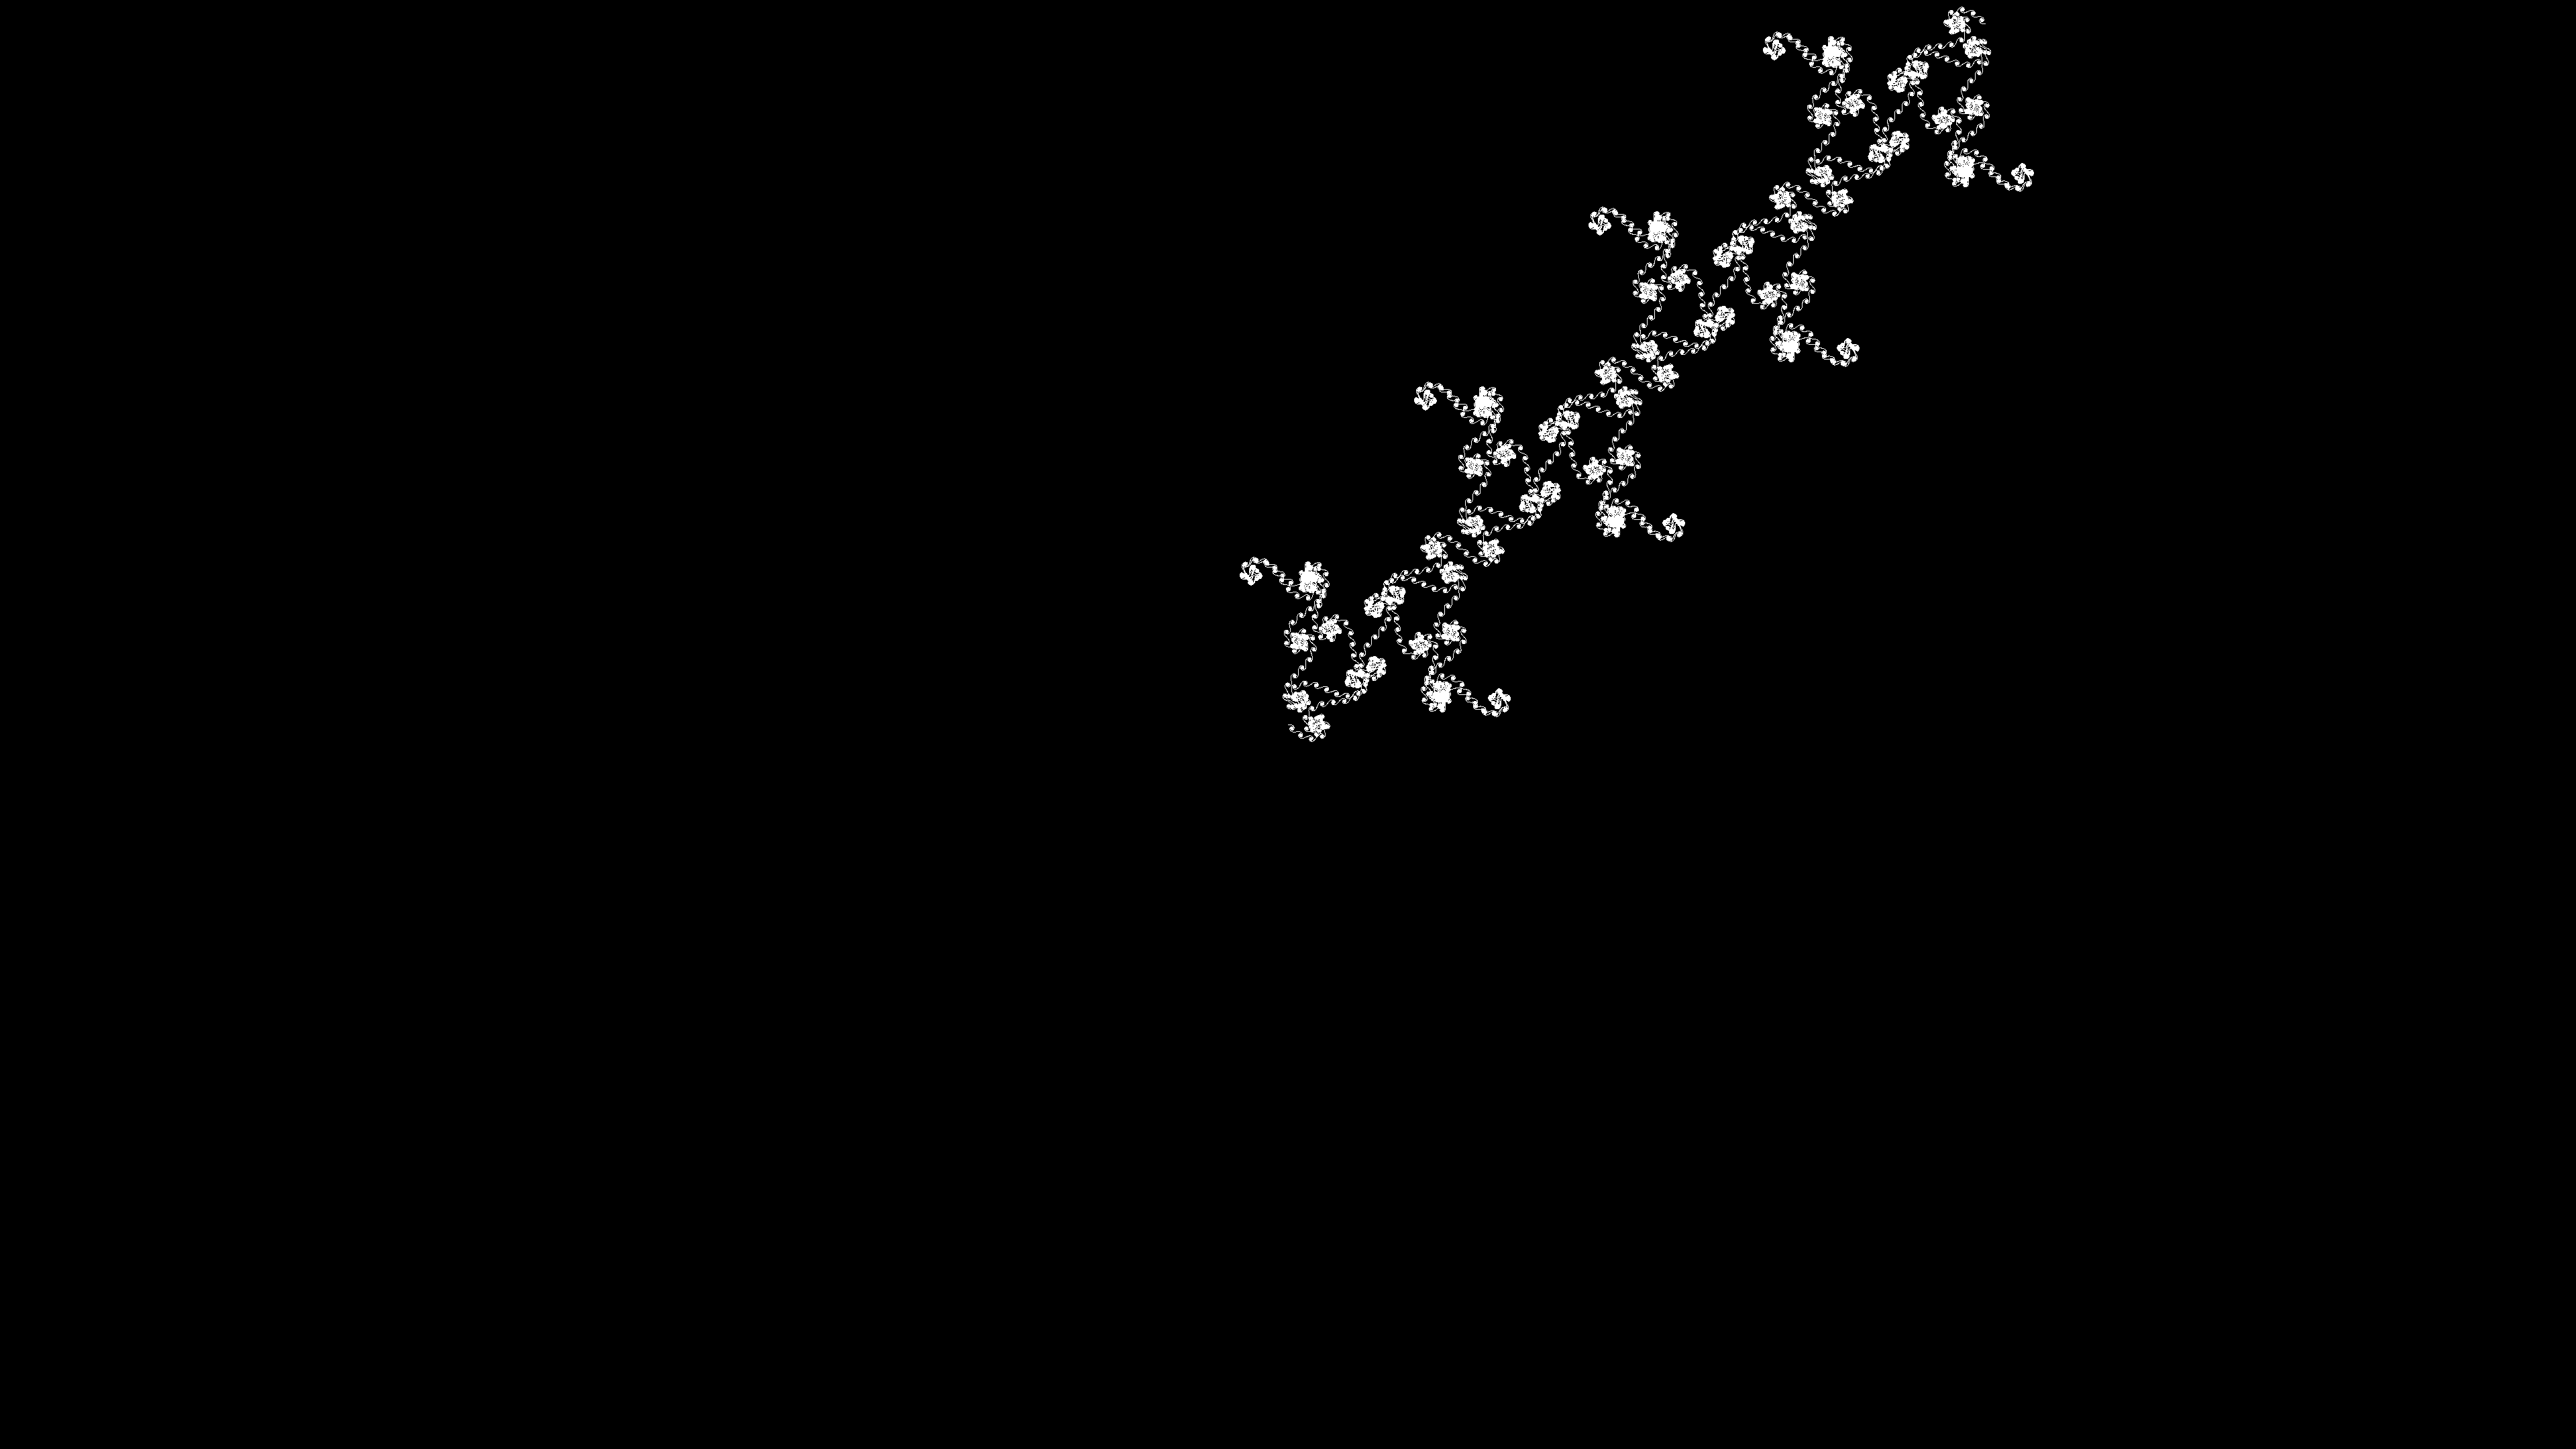
\includegraphics[width=\linewidth]{./stepsplusoneimages/0000000020.png}
    \caption{tf p=499 q=200117 theta=000 89767486.png}
  \end{subfigure}
  \caption{n=018 s=400 s+1=401}
  \label{fig:n=018}
\end{figure}
\begin{figure}[H]
  \centering
  \begin{subfigure}[t]{0.48\textwidth}
    \centering
    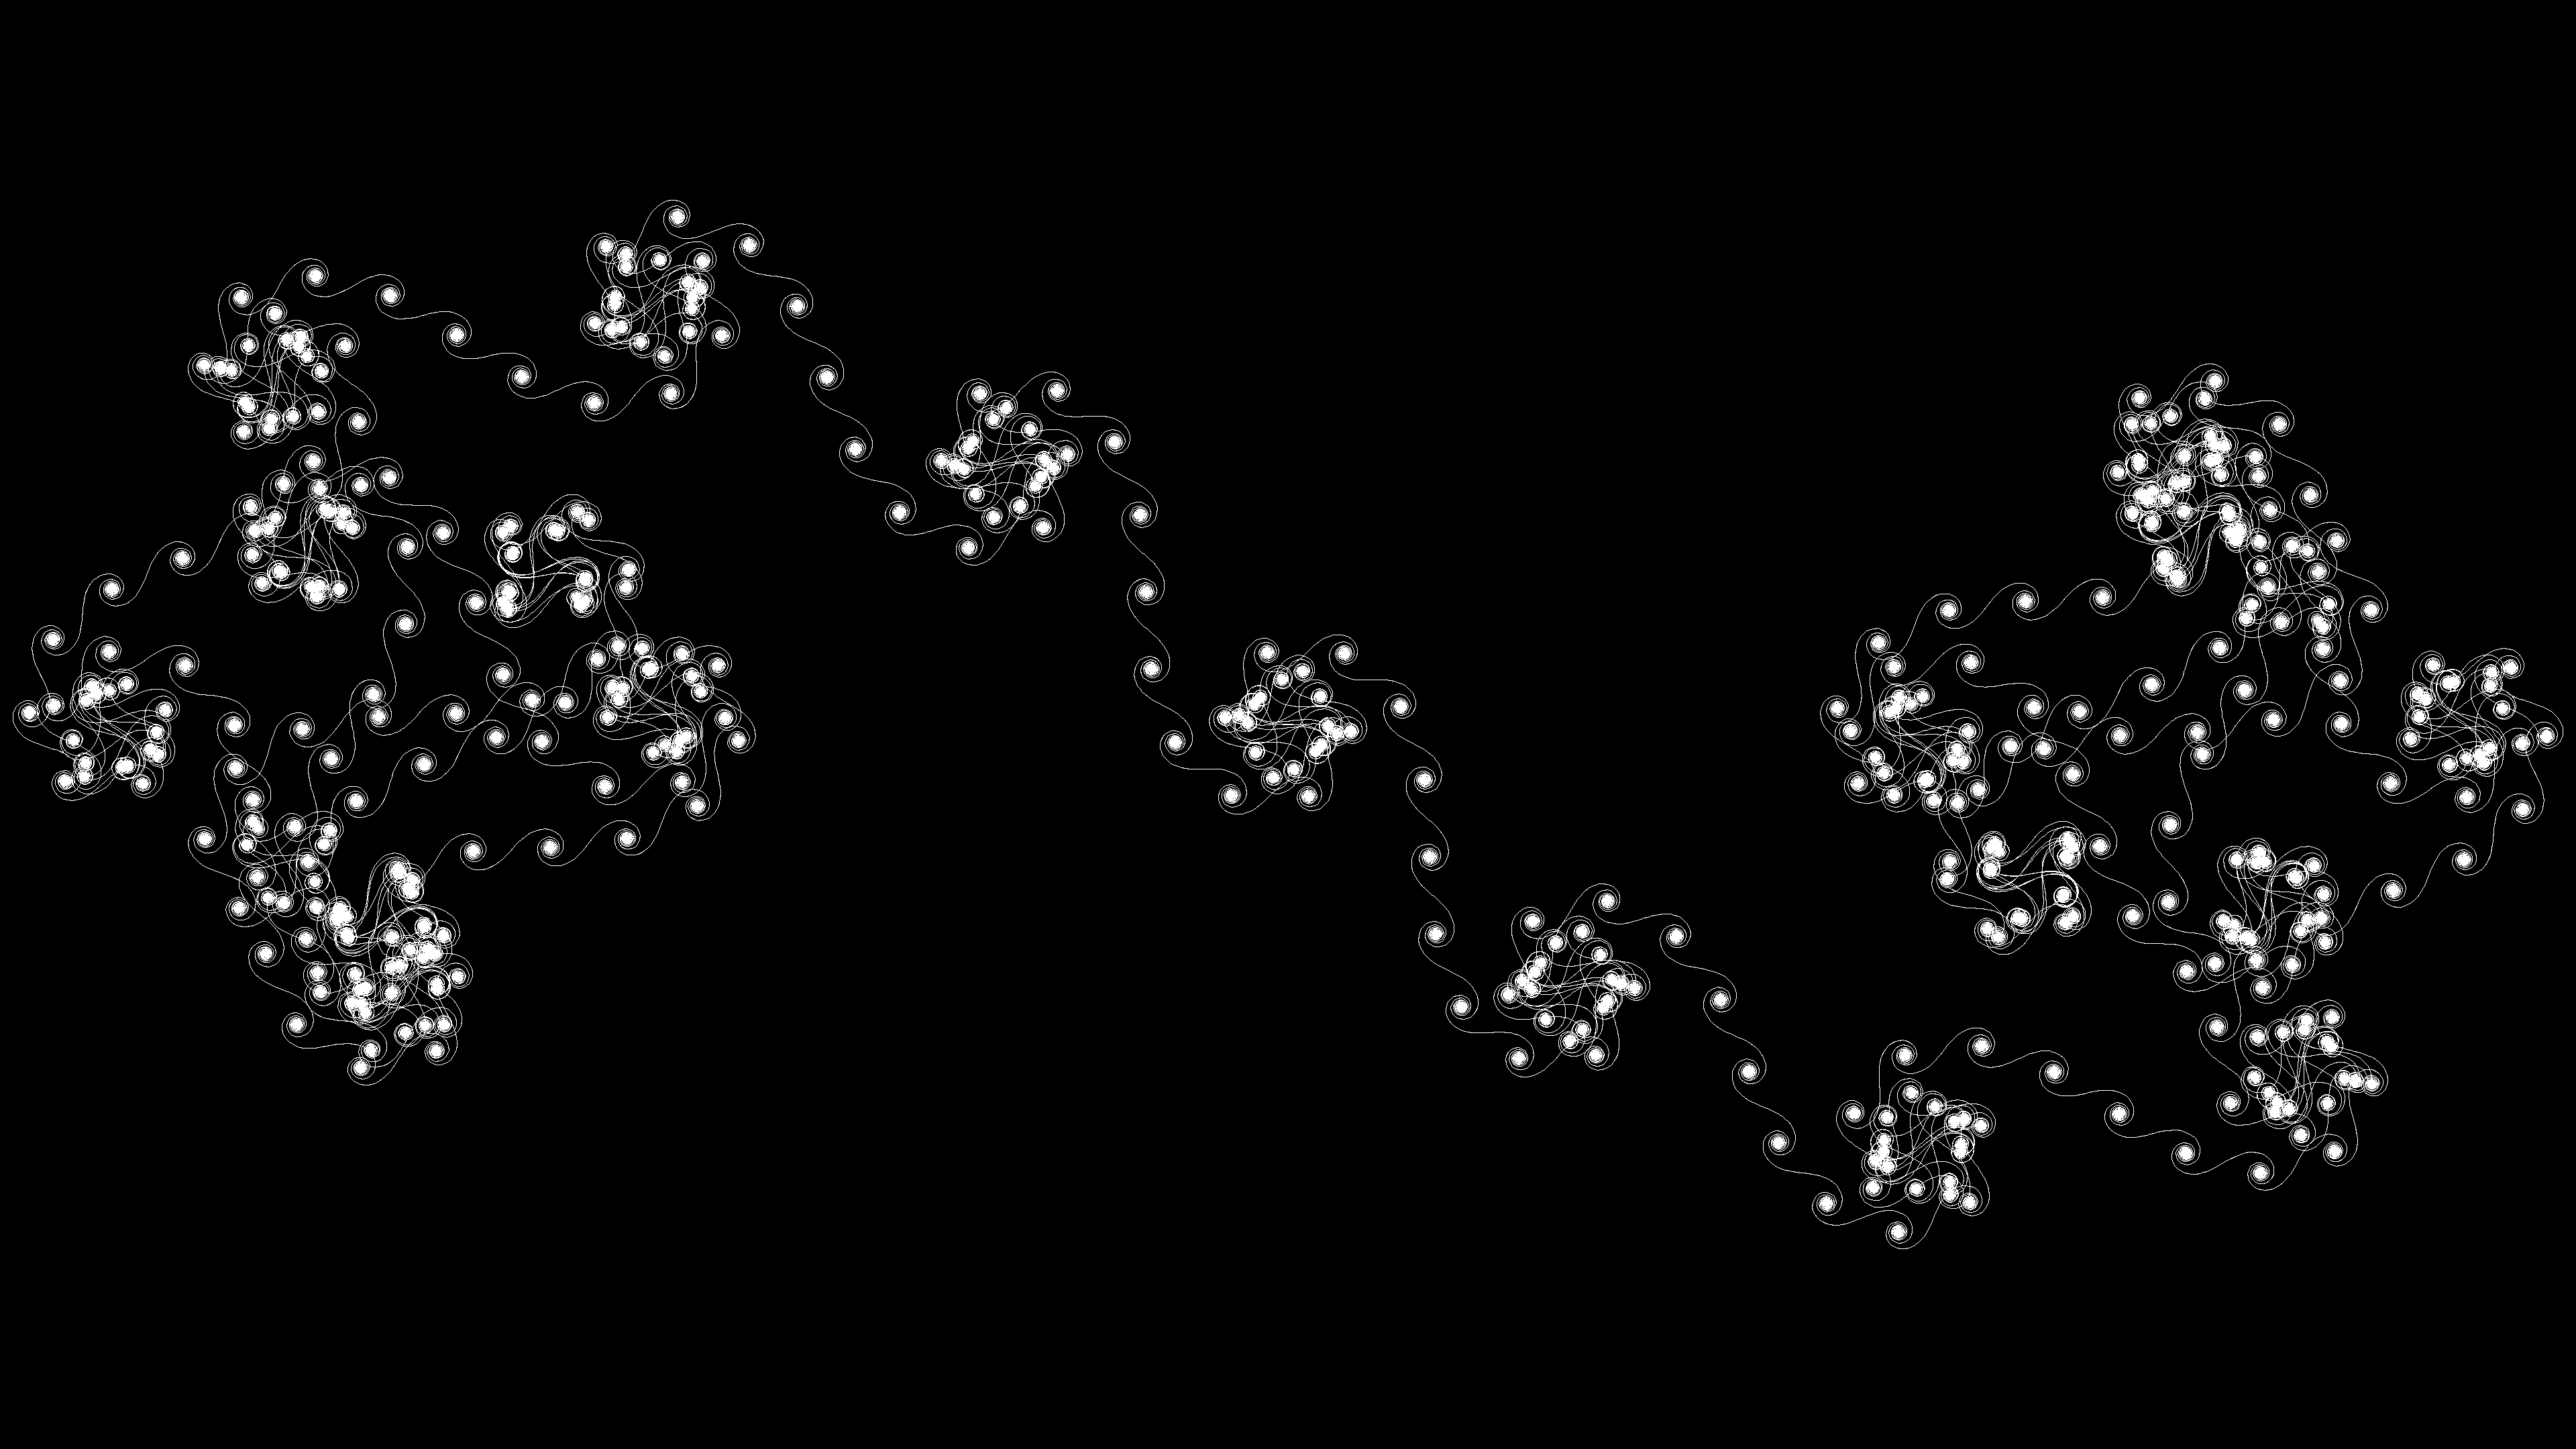
\includegraphics[width=\linewidth]{./stepsplusoneimages/0000000021.png}
    \caption{tf p=499 q=199620 theta=000 89990983.png}
  \end{subfigure}
  \begin{subfigure}[t]{0.48\textwidth}
    \centering
    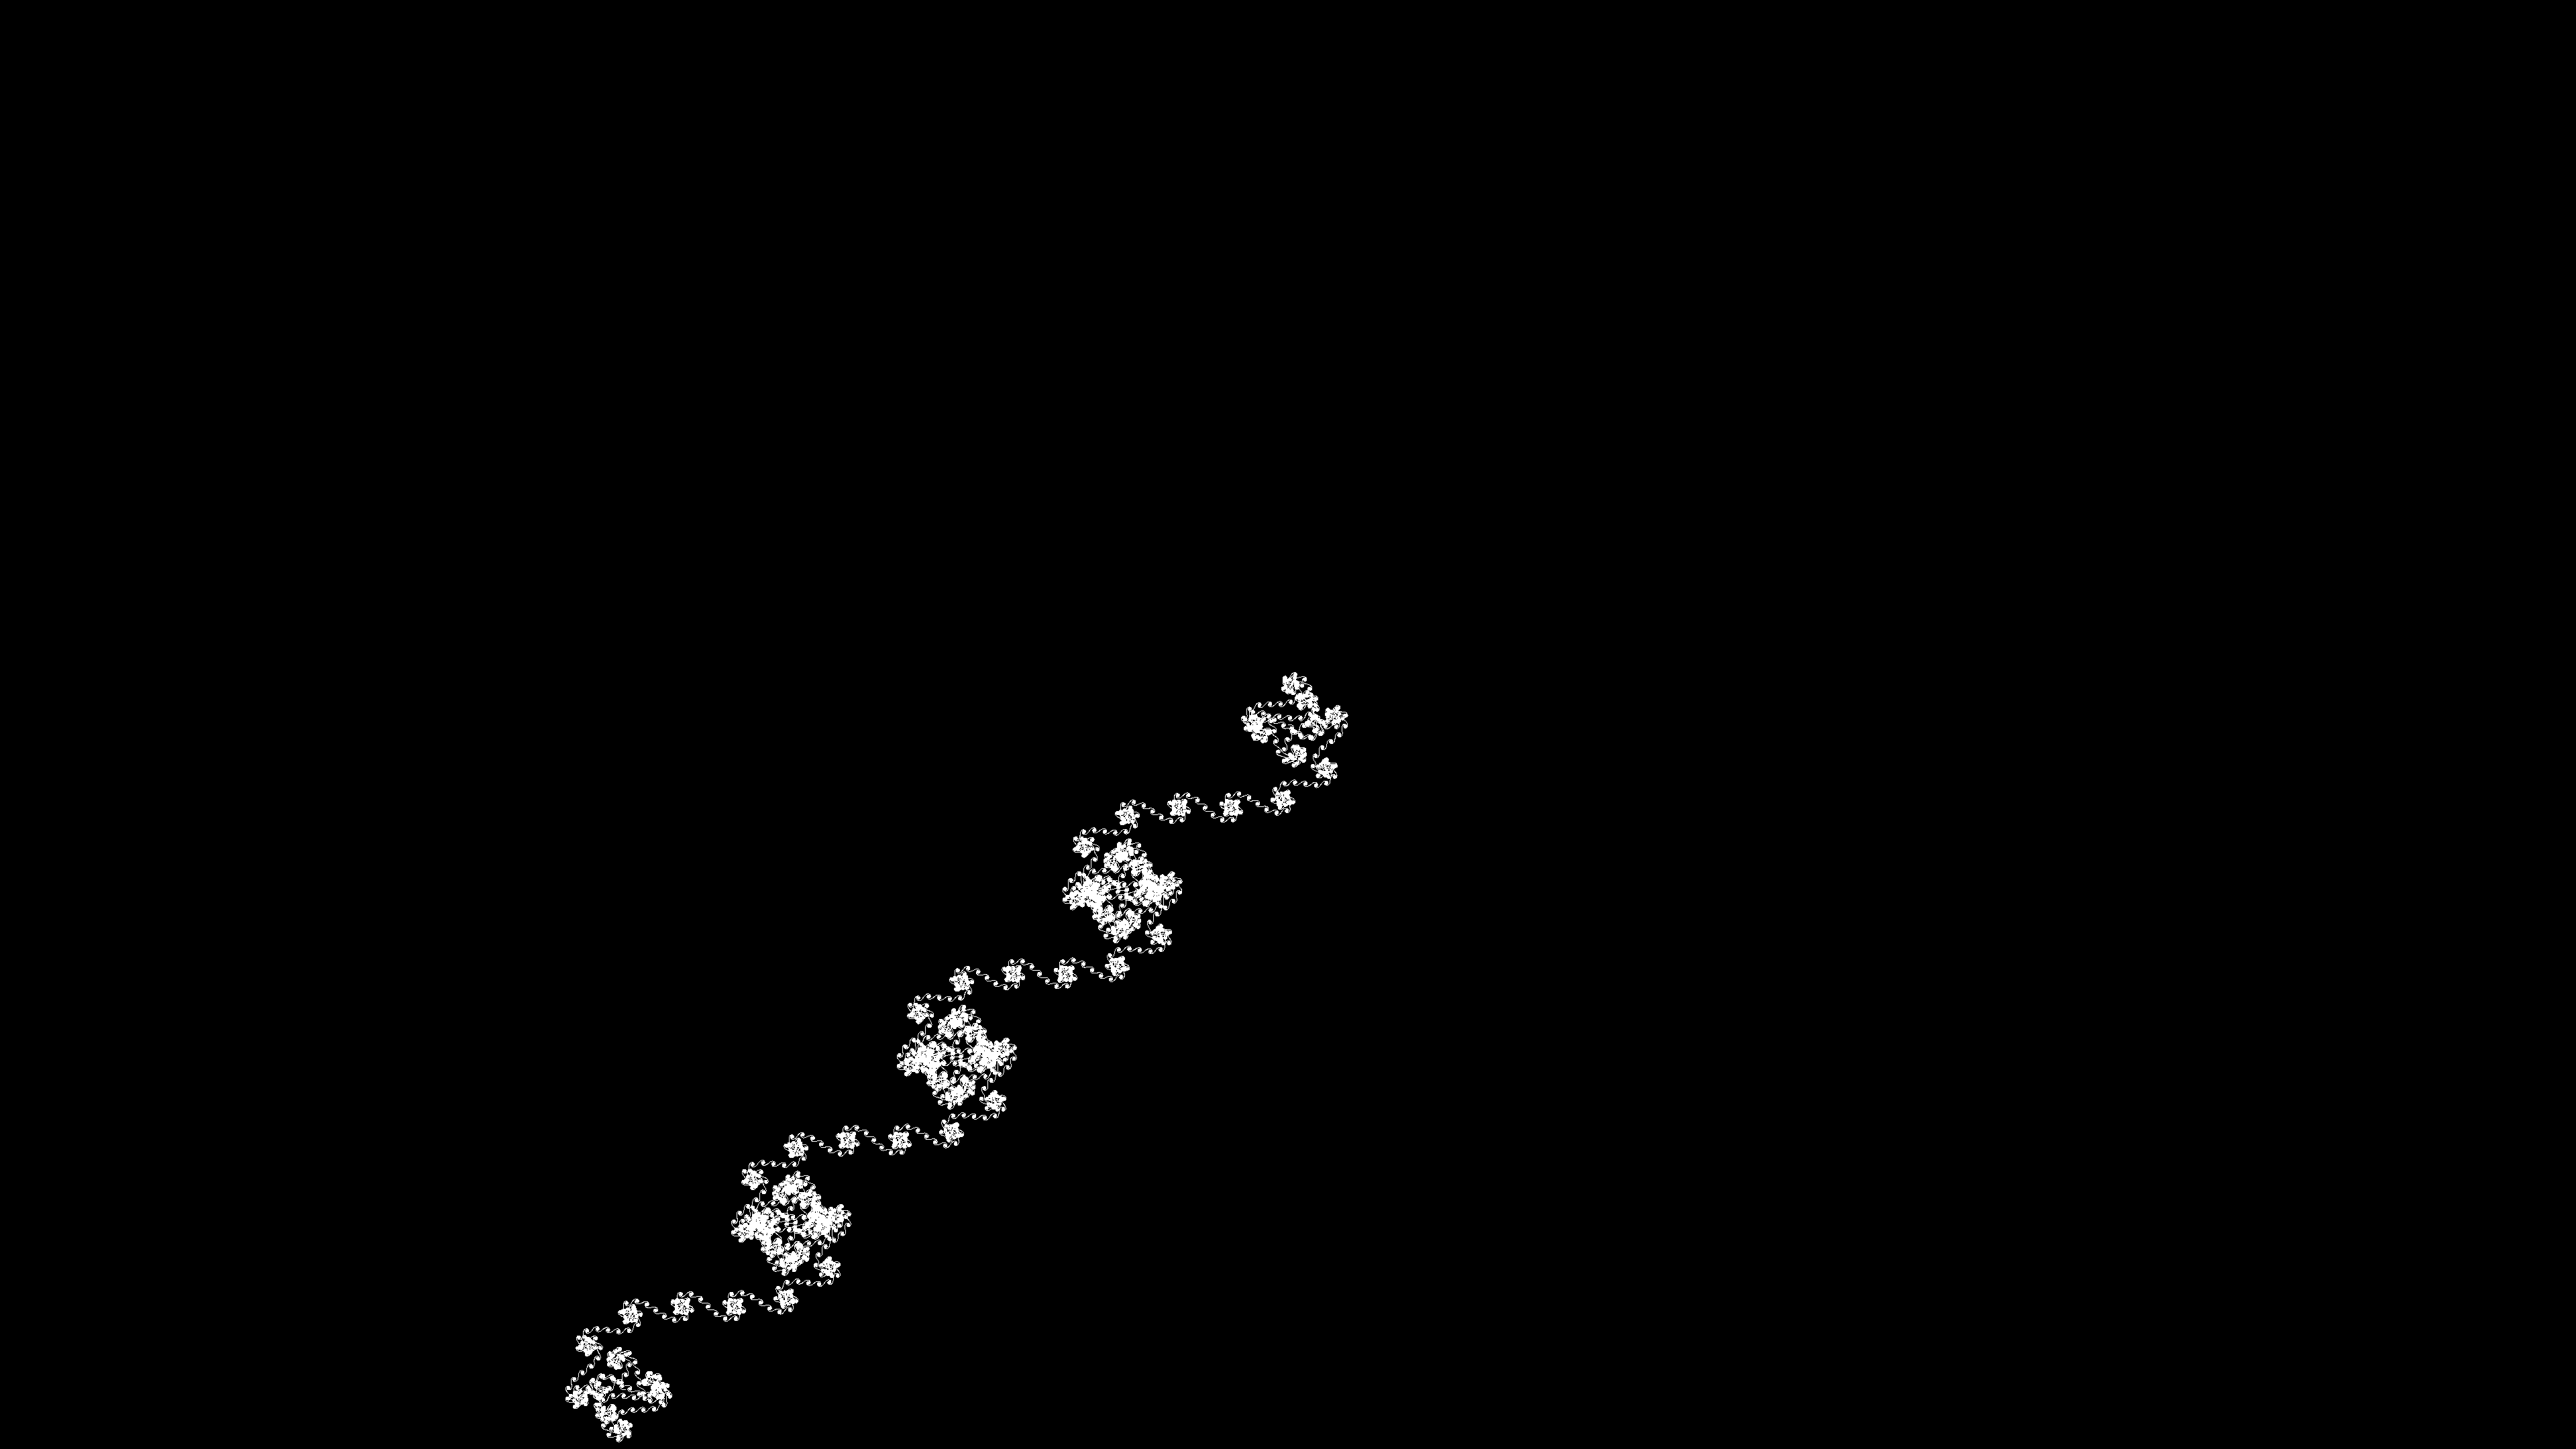
\includegraphics[width=\linewidth]{./stepsplusoneimages/0000000022.png}
    \caption{tf p=499 q=200119 theta=000 89766589.png}
  \end{subfigure}
  \caption{n=020 s=400 s+1=401}
  \label{fig:n=020}
\end{figure}
\begin{figure}[H]
  \centering
  \begin{subfigure}[t]{0.48\textwidth}
    \centering
    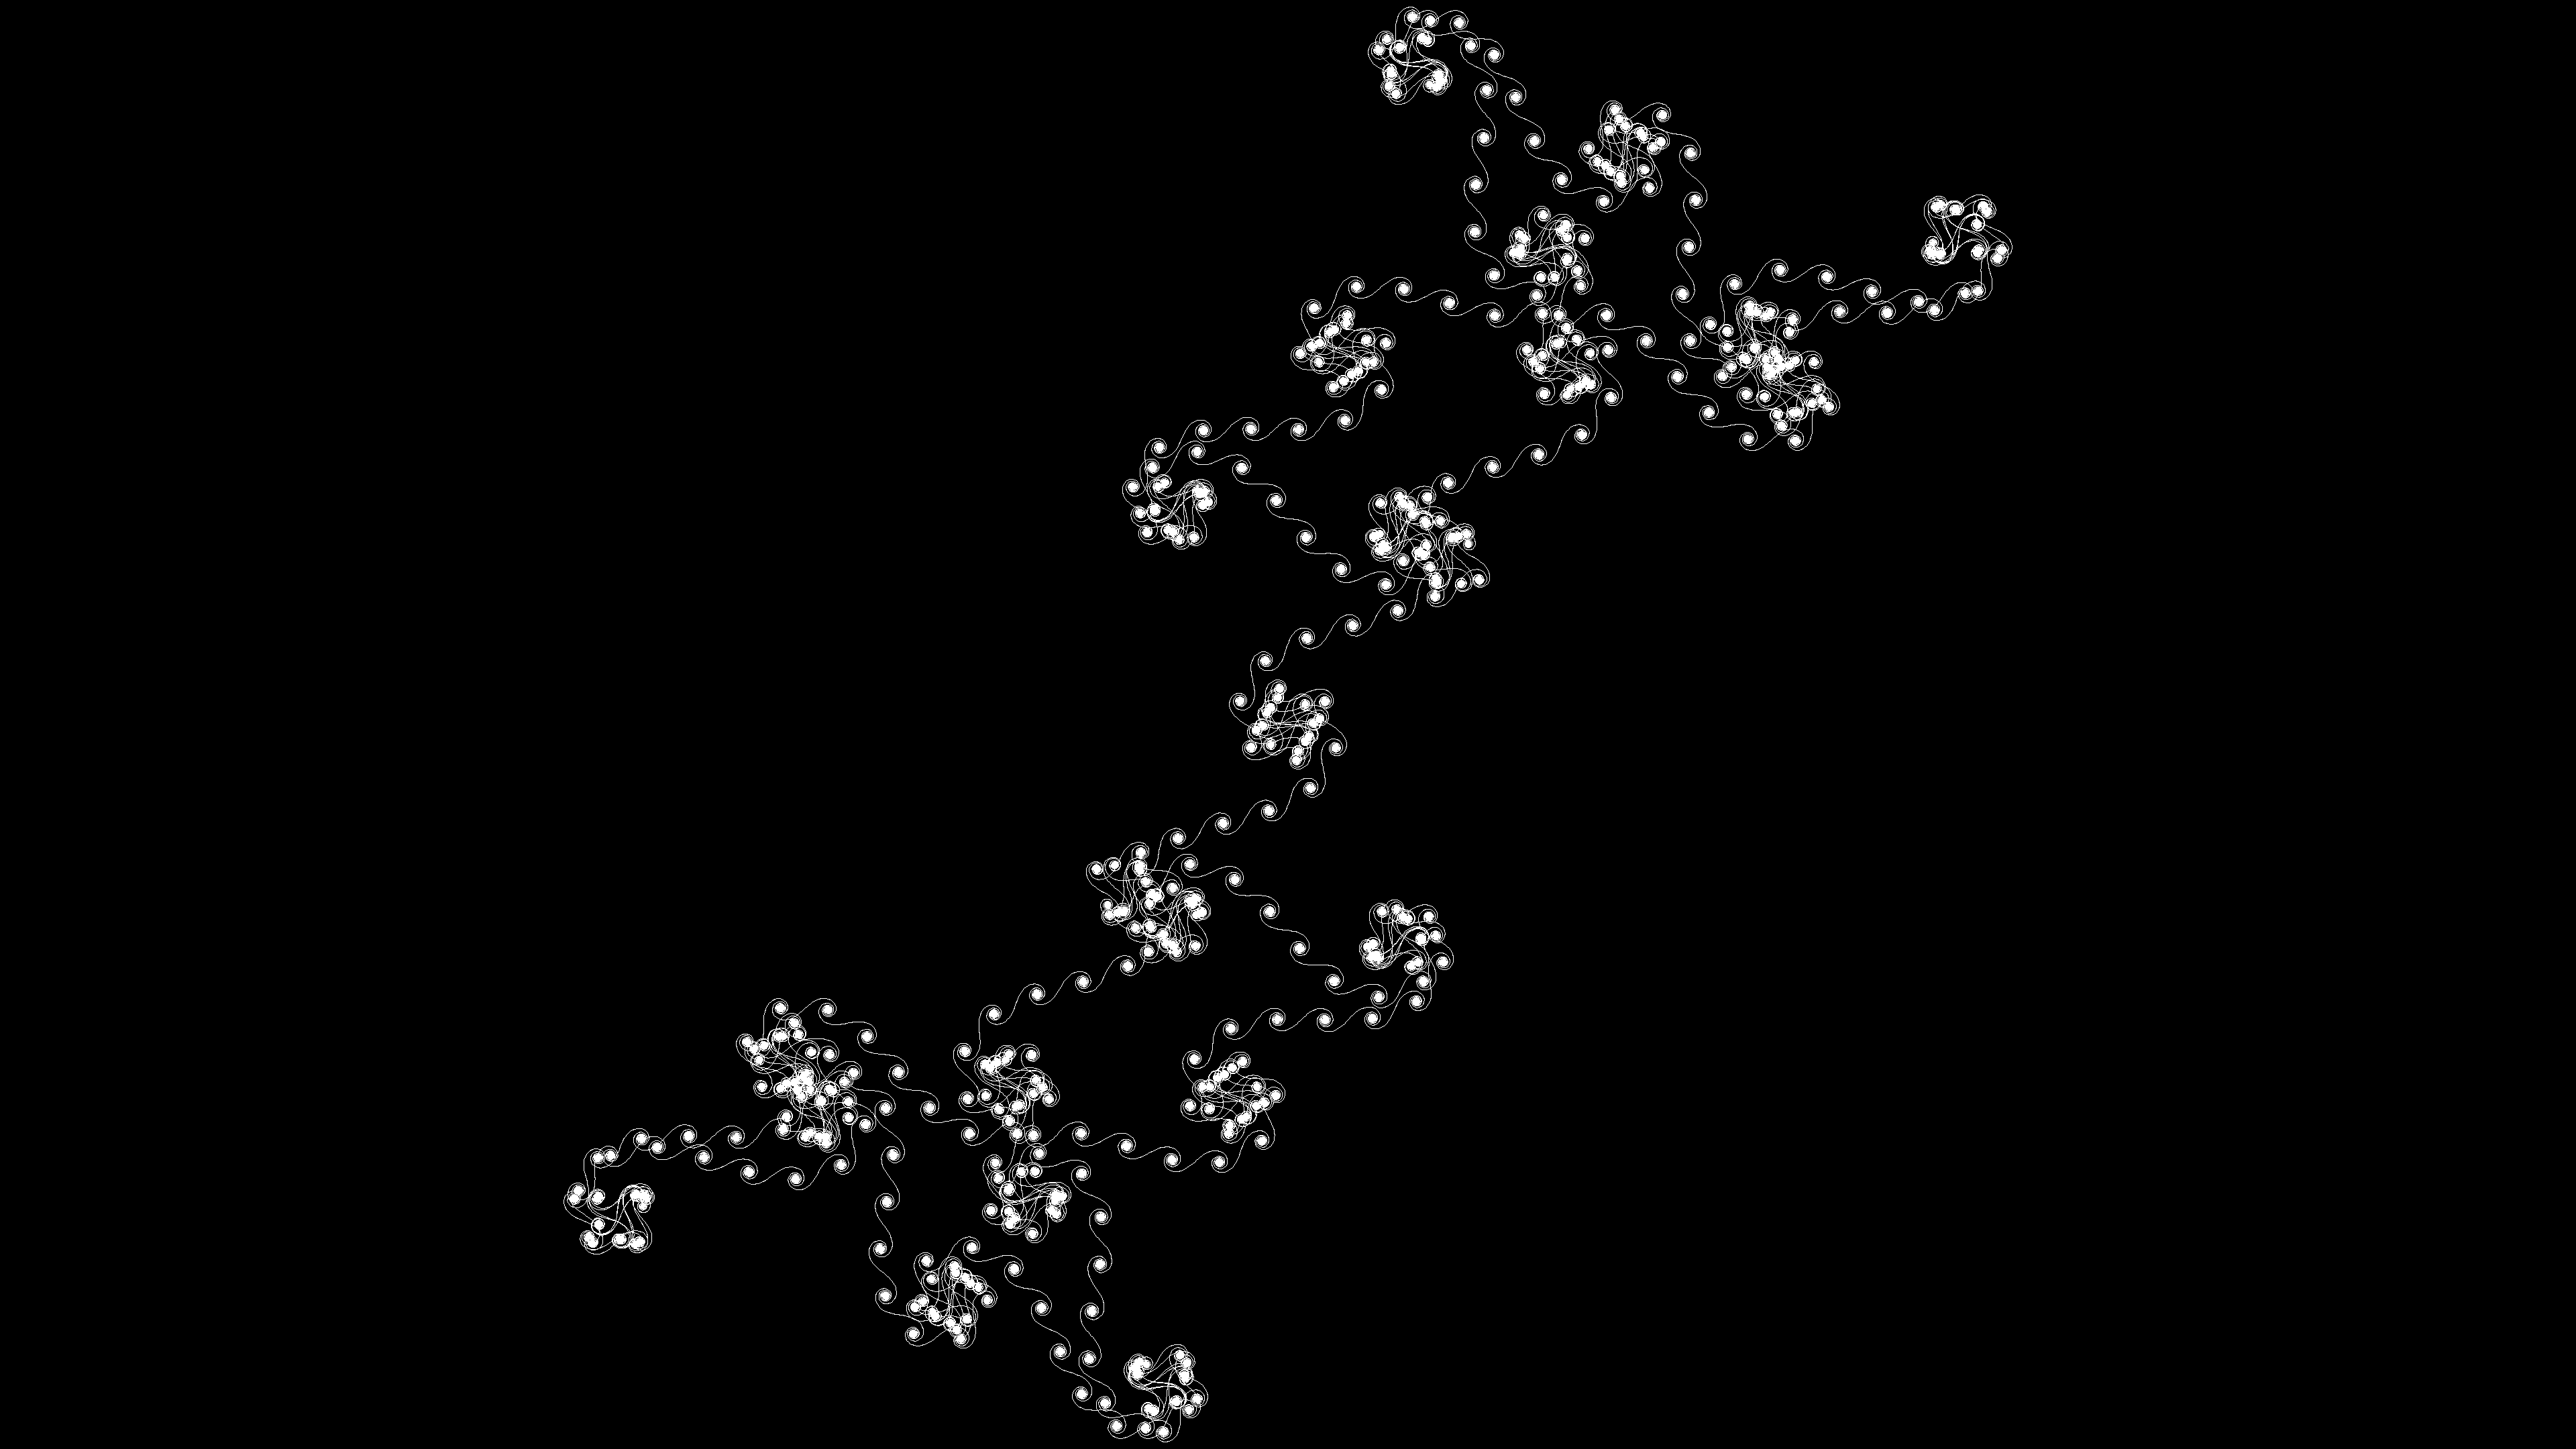
\includegraphics[width=\linewidth]{./stepsplusoneimages/0000000023.png}
    \caption{tf p=499 q=199622 theta=000 89990081.png}
  \end{subfigure}
  \begin{subfigure}[t]{0.48\textwidth}
    \centering
    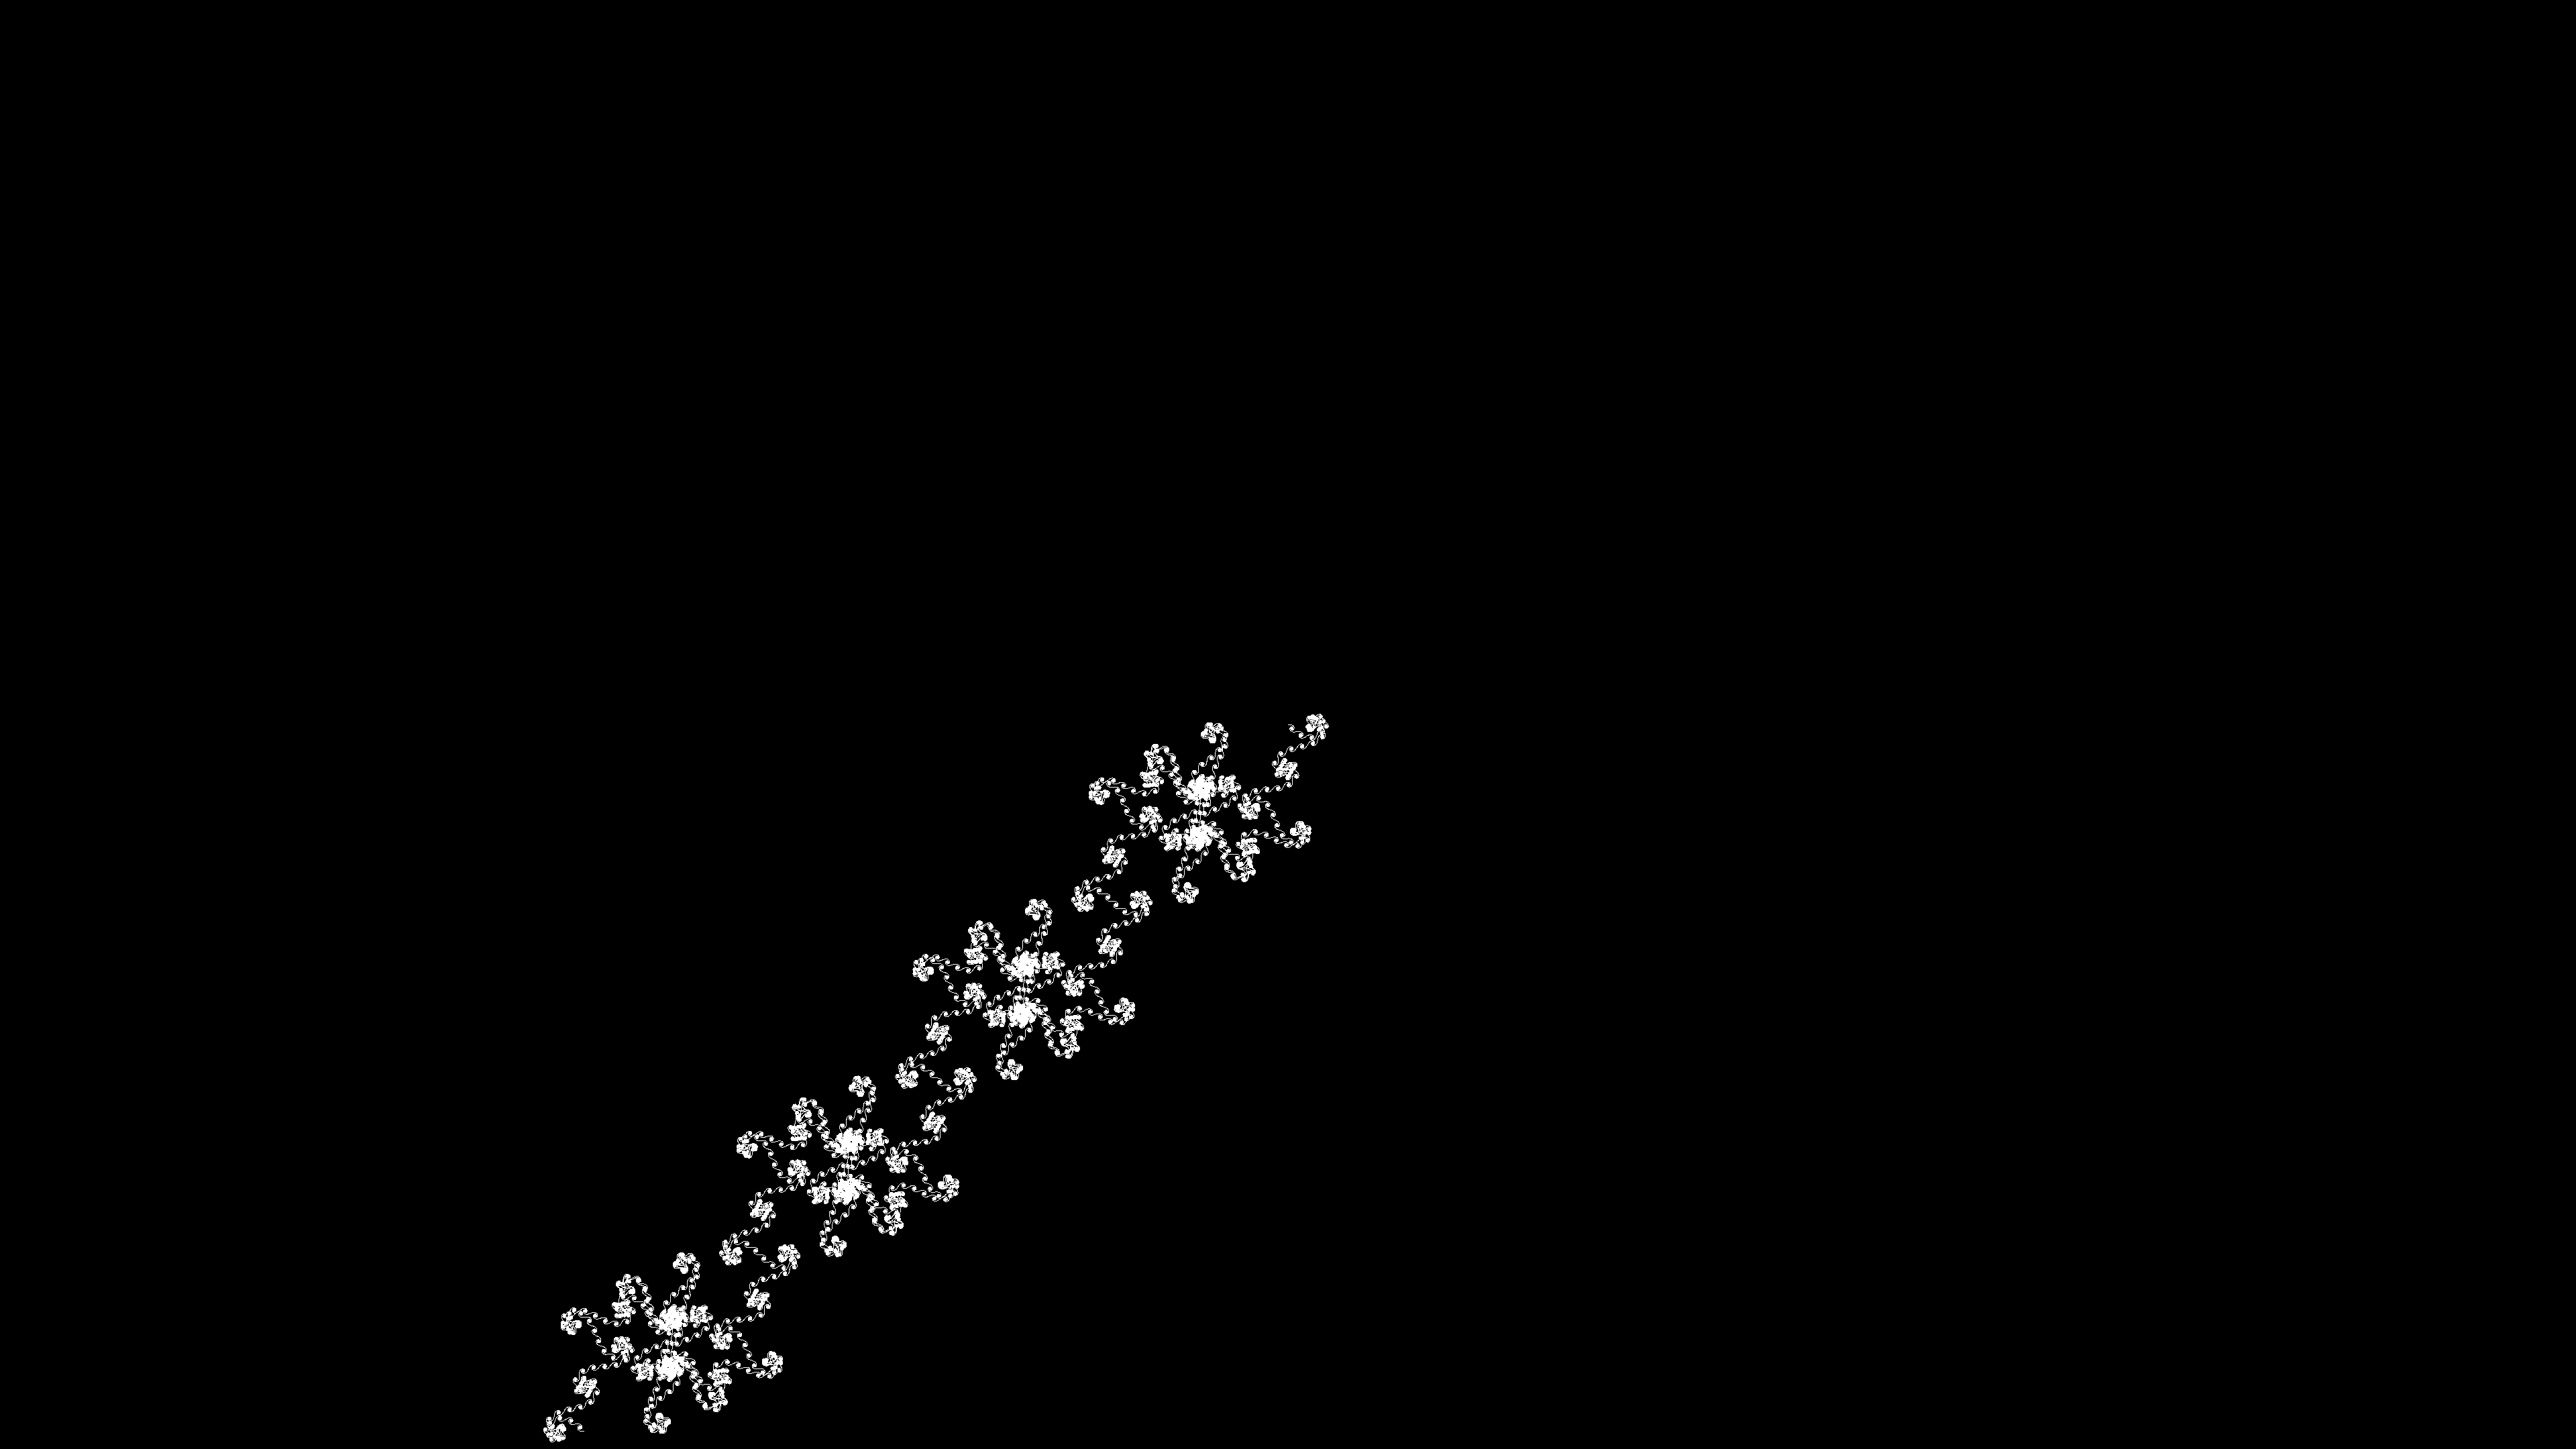
\includegraphics[width=\linewidth]{./stepsplusoneimages/0000000024.png}
    \caption{tf p=499 q=200121 theta=000 89765692.png}
  \end{subfigure}
  \caption{n=022 s=400 s+1=401}
  \label{fig:n=022}
\end{figure}
\begin{figure}[H]
  \centering
  \begin{subfigure}[t]{0.48\textwidth}
    \centering
    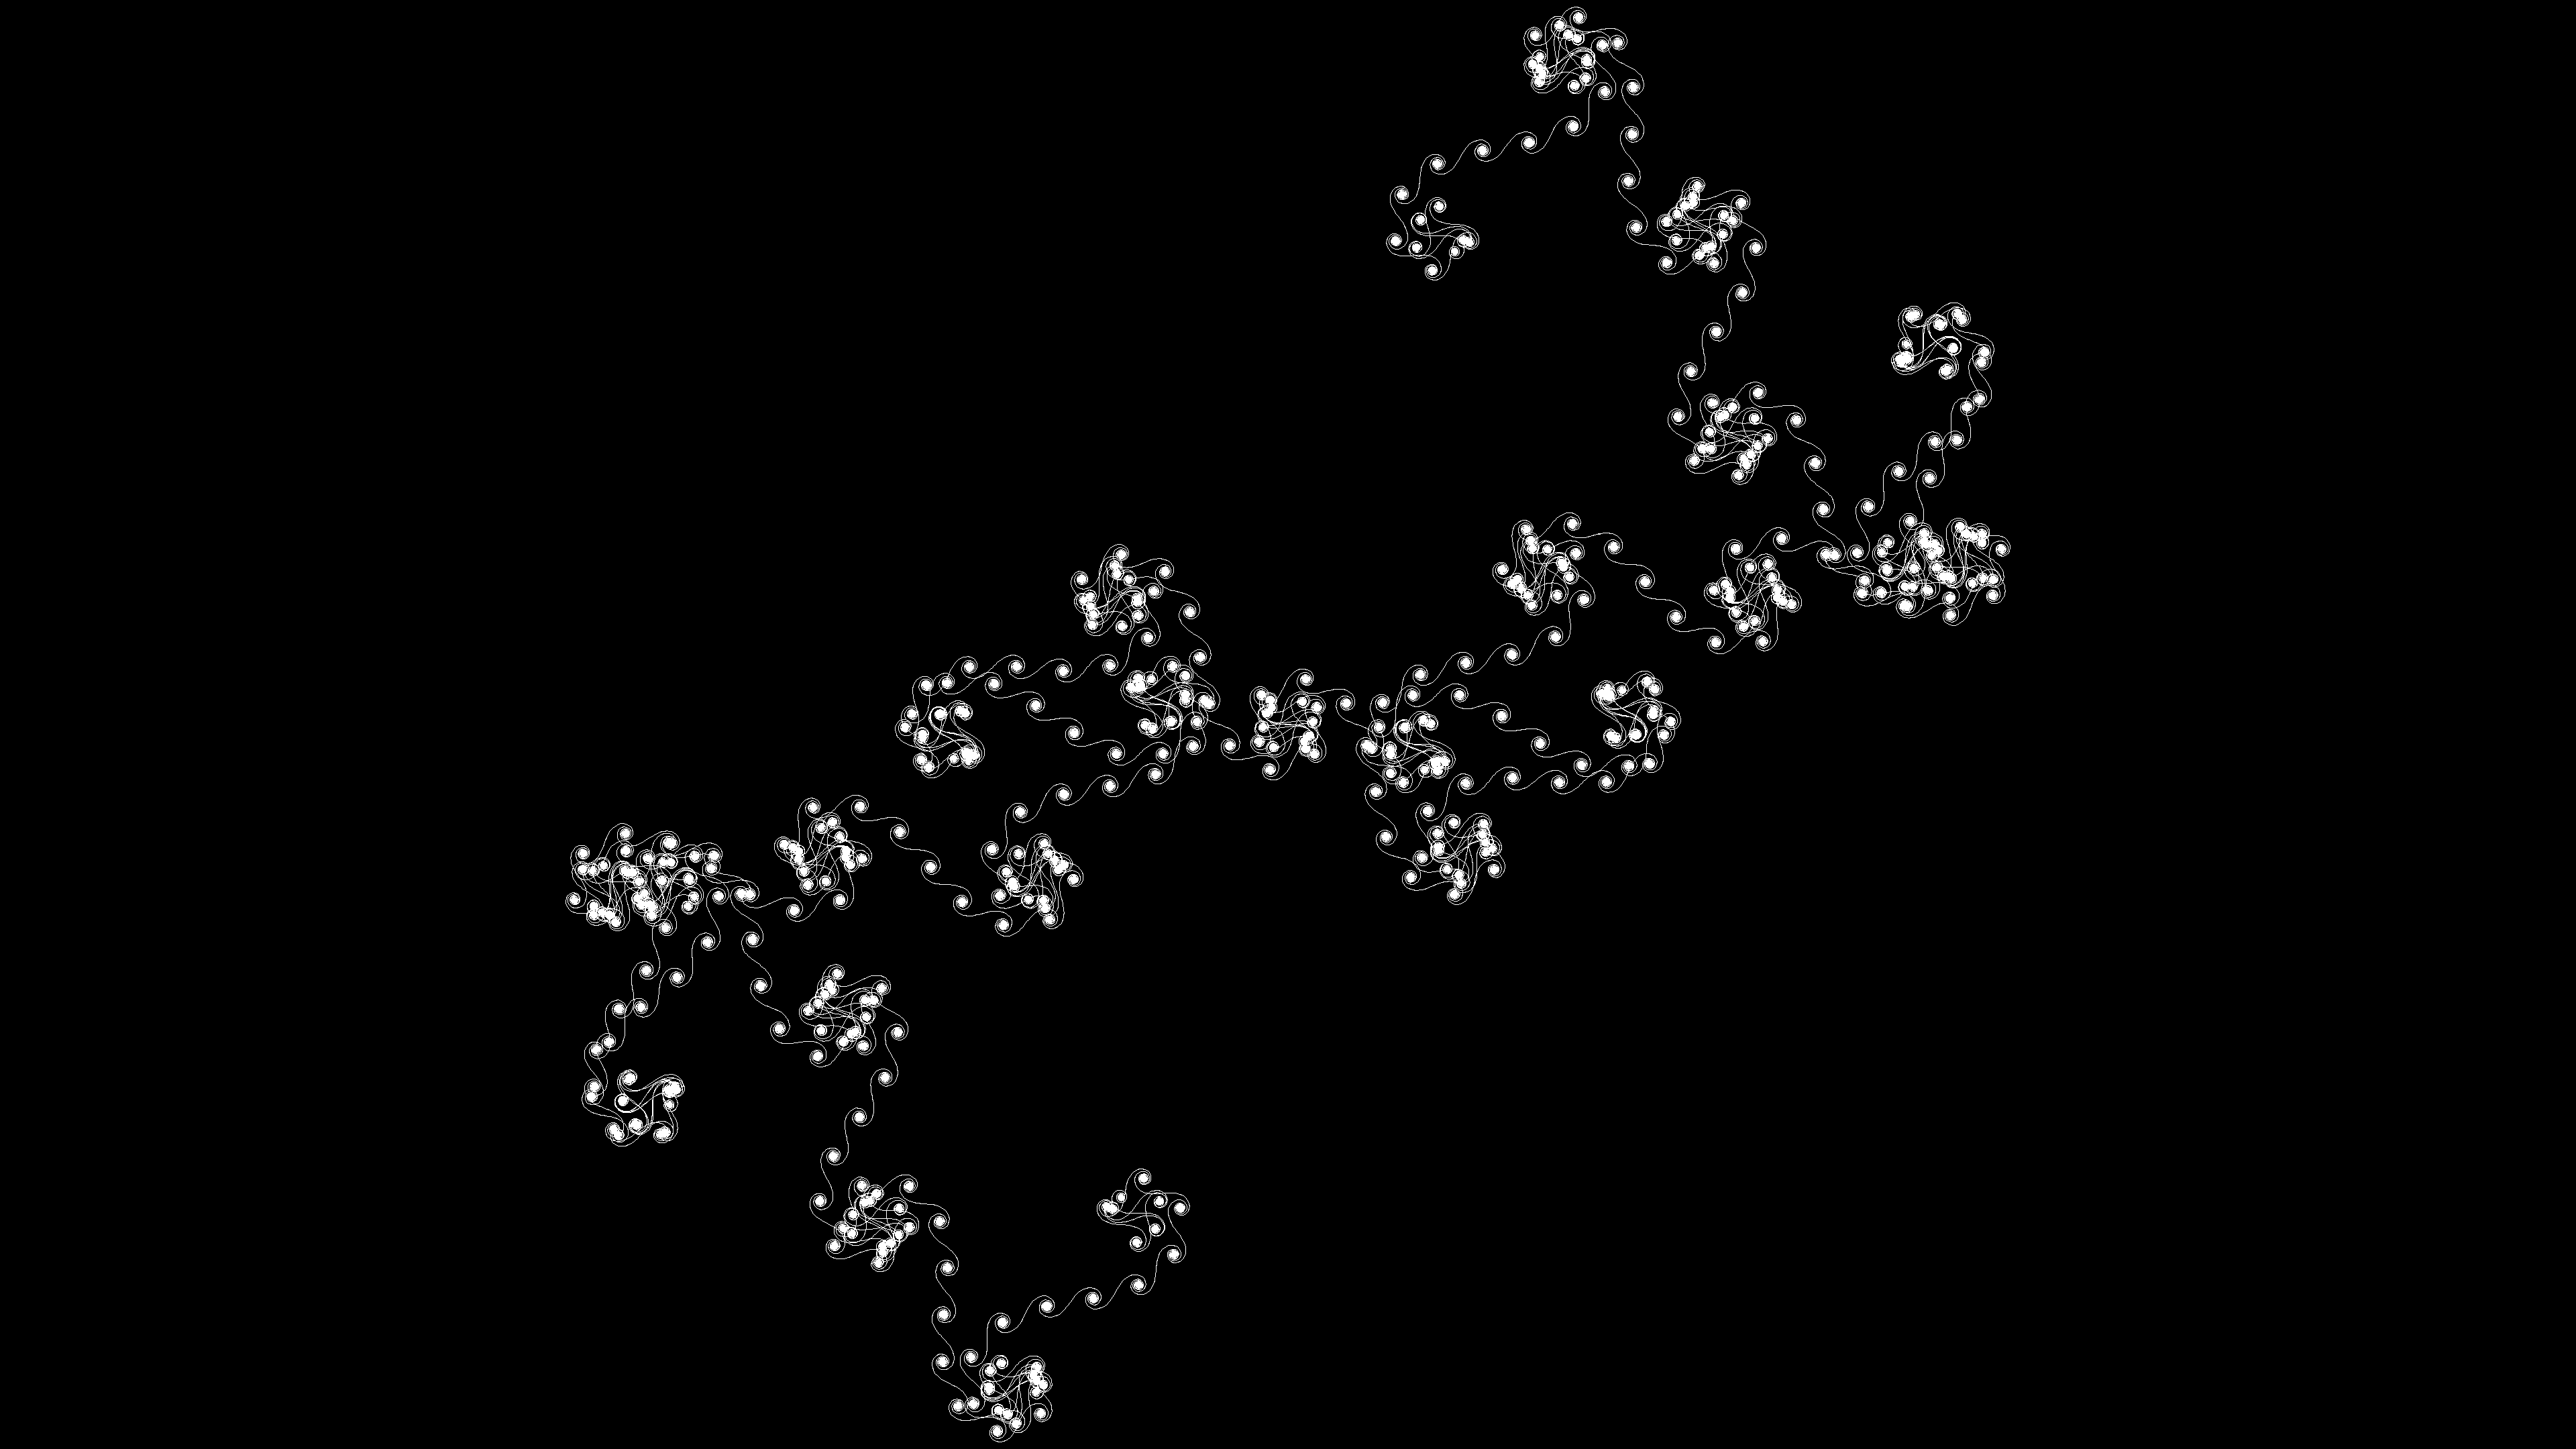
\includegraphics[width=\linewidth]{./stepsplusoneimages/0000000025.png}
    \caption{tf p=499 q=199624 theta=000 89989180.png}
  \end{subfigure}
  \begin{subfigure}[t]{0.48\textwidth}
    \centering
    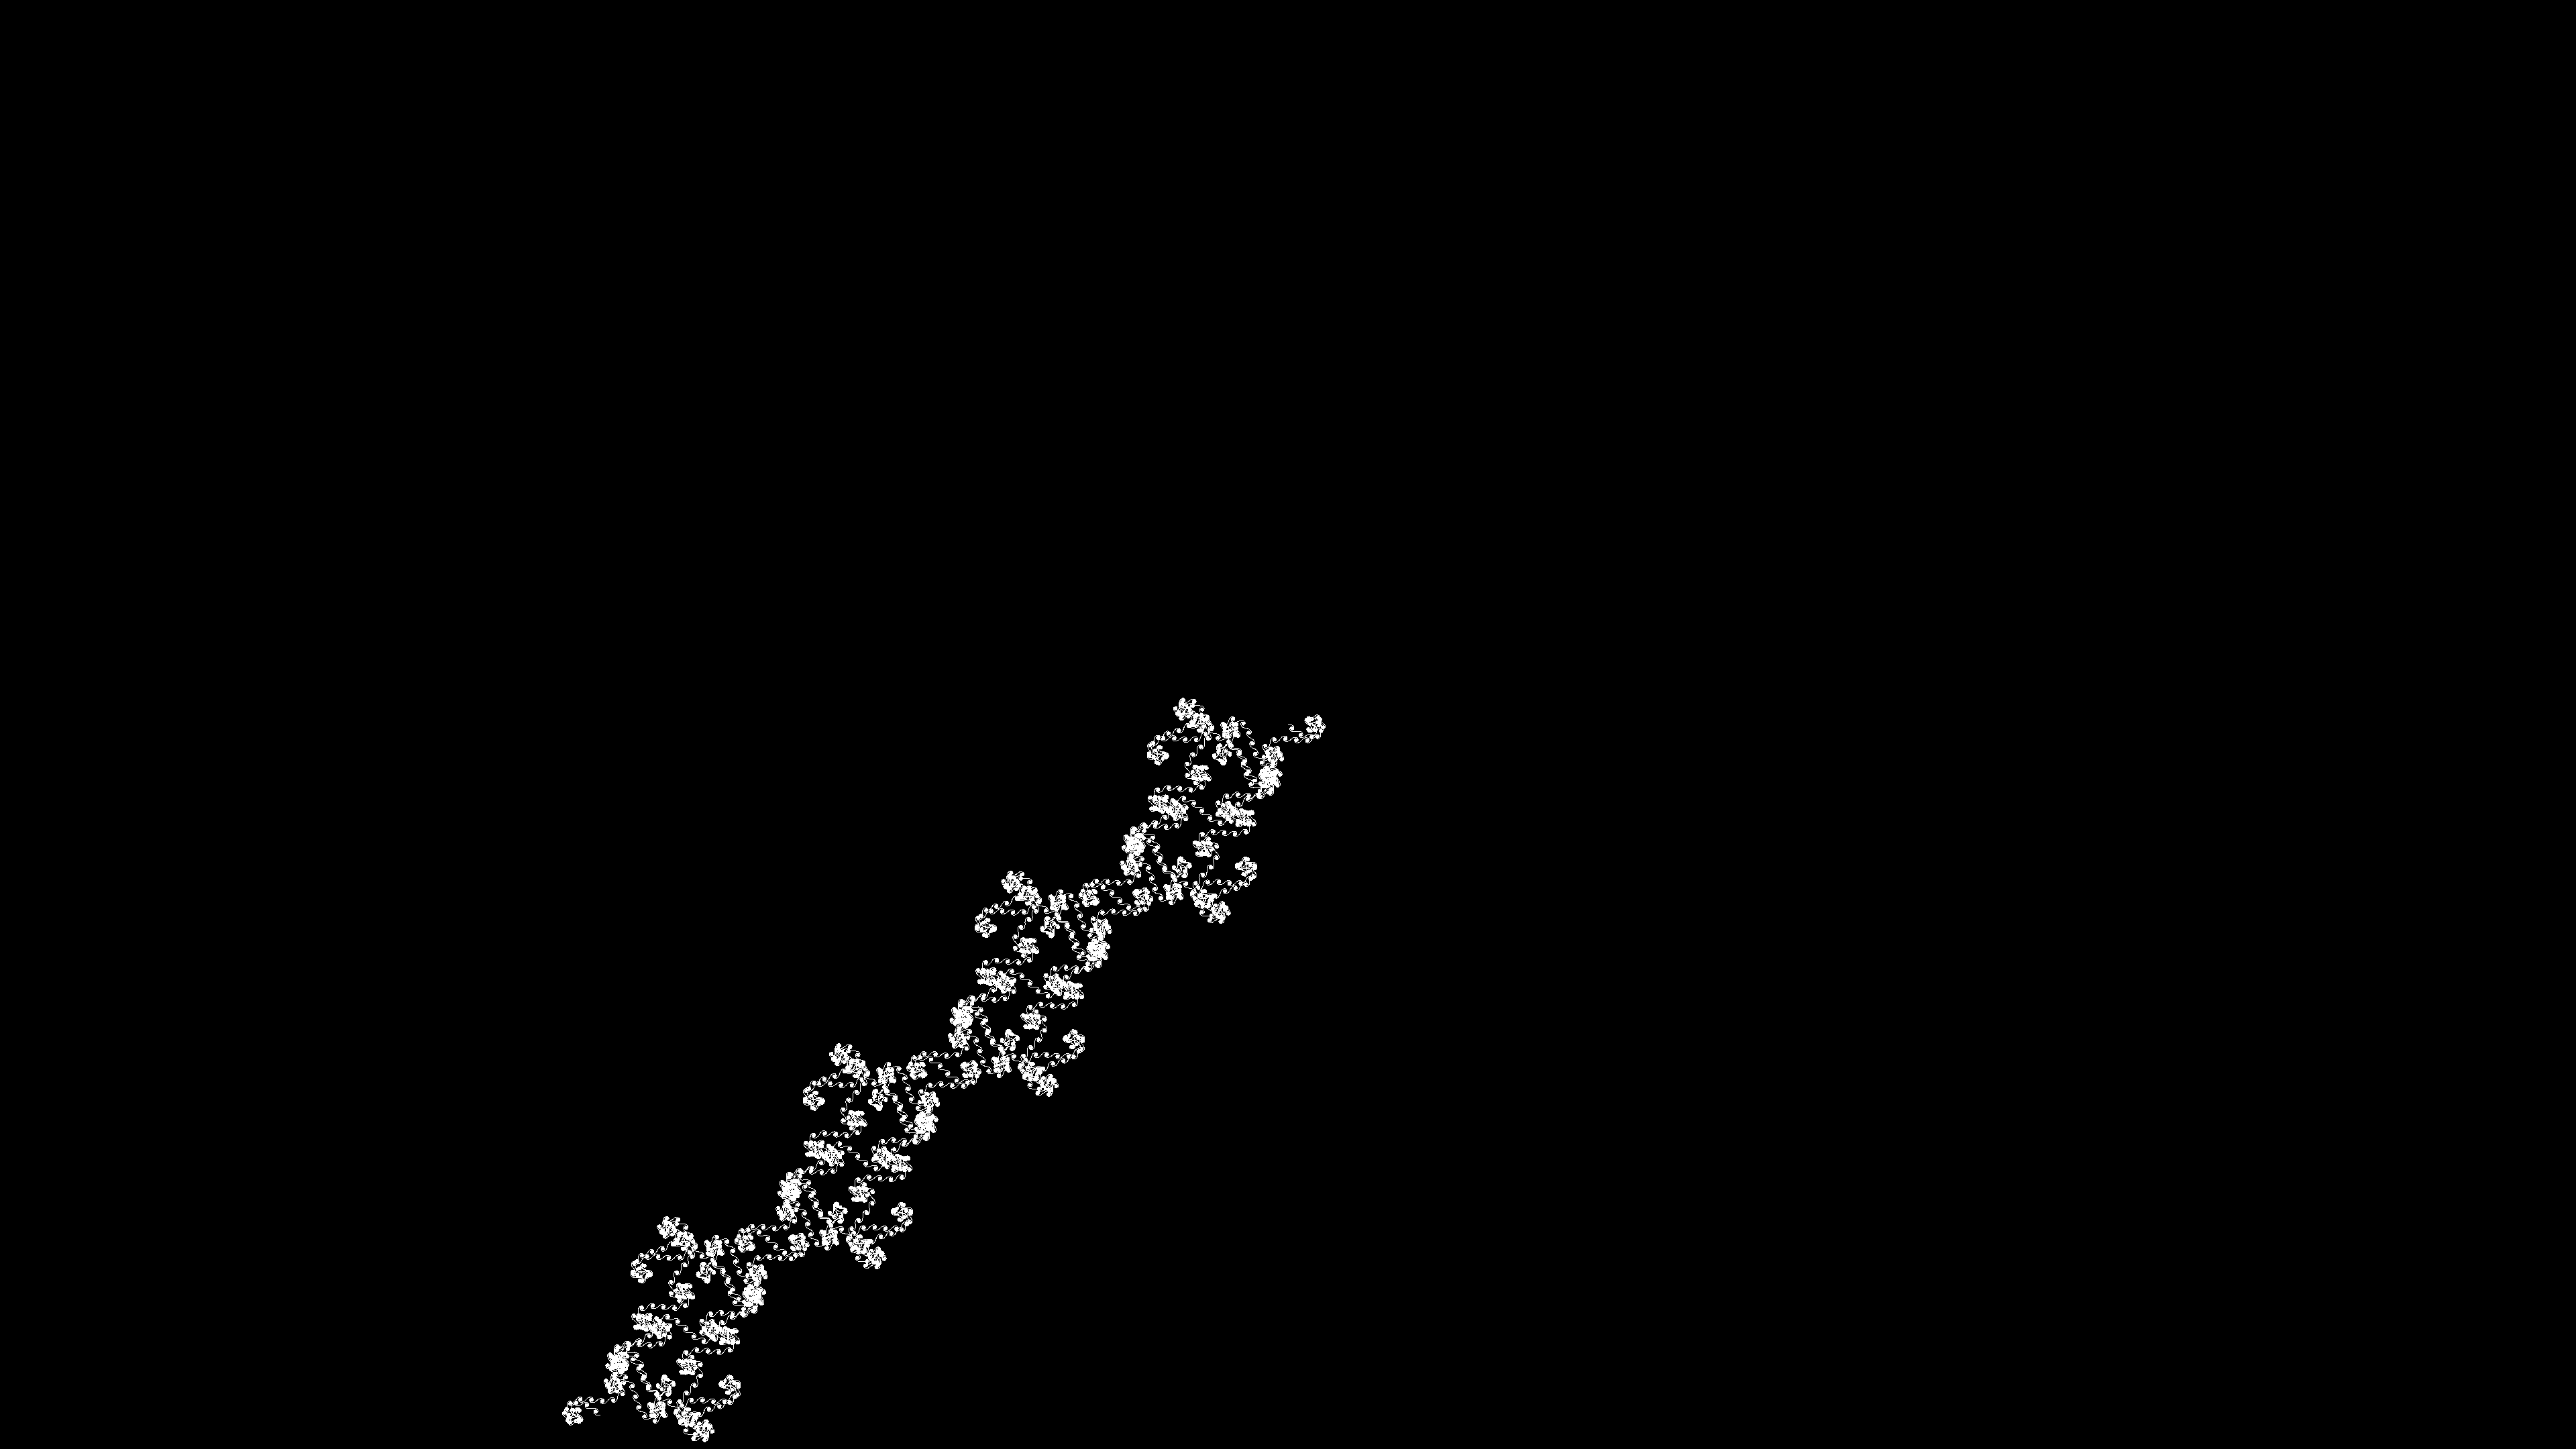
\includegraphics[width=\linewidth]{./stepsplusoneimages/0000000026.png}
    \caption{tf p=499 q=200123 theta=000 89764795.png}
  \end{subfigure}
  \caption{n=024 s=400 s+1=401}
  \label{fig:n=024}
\end{figure}
\begin{figure}[H]
  \centering
  \begin{subfigure}[t]{0.48\textwidth}
    \centering
    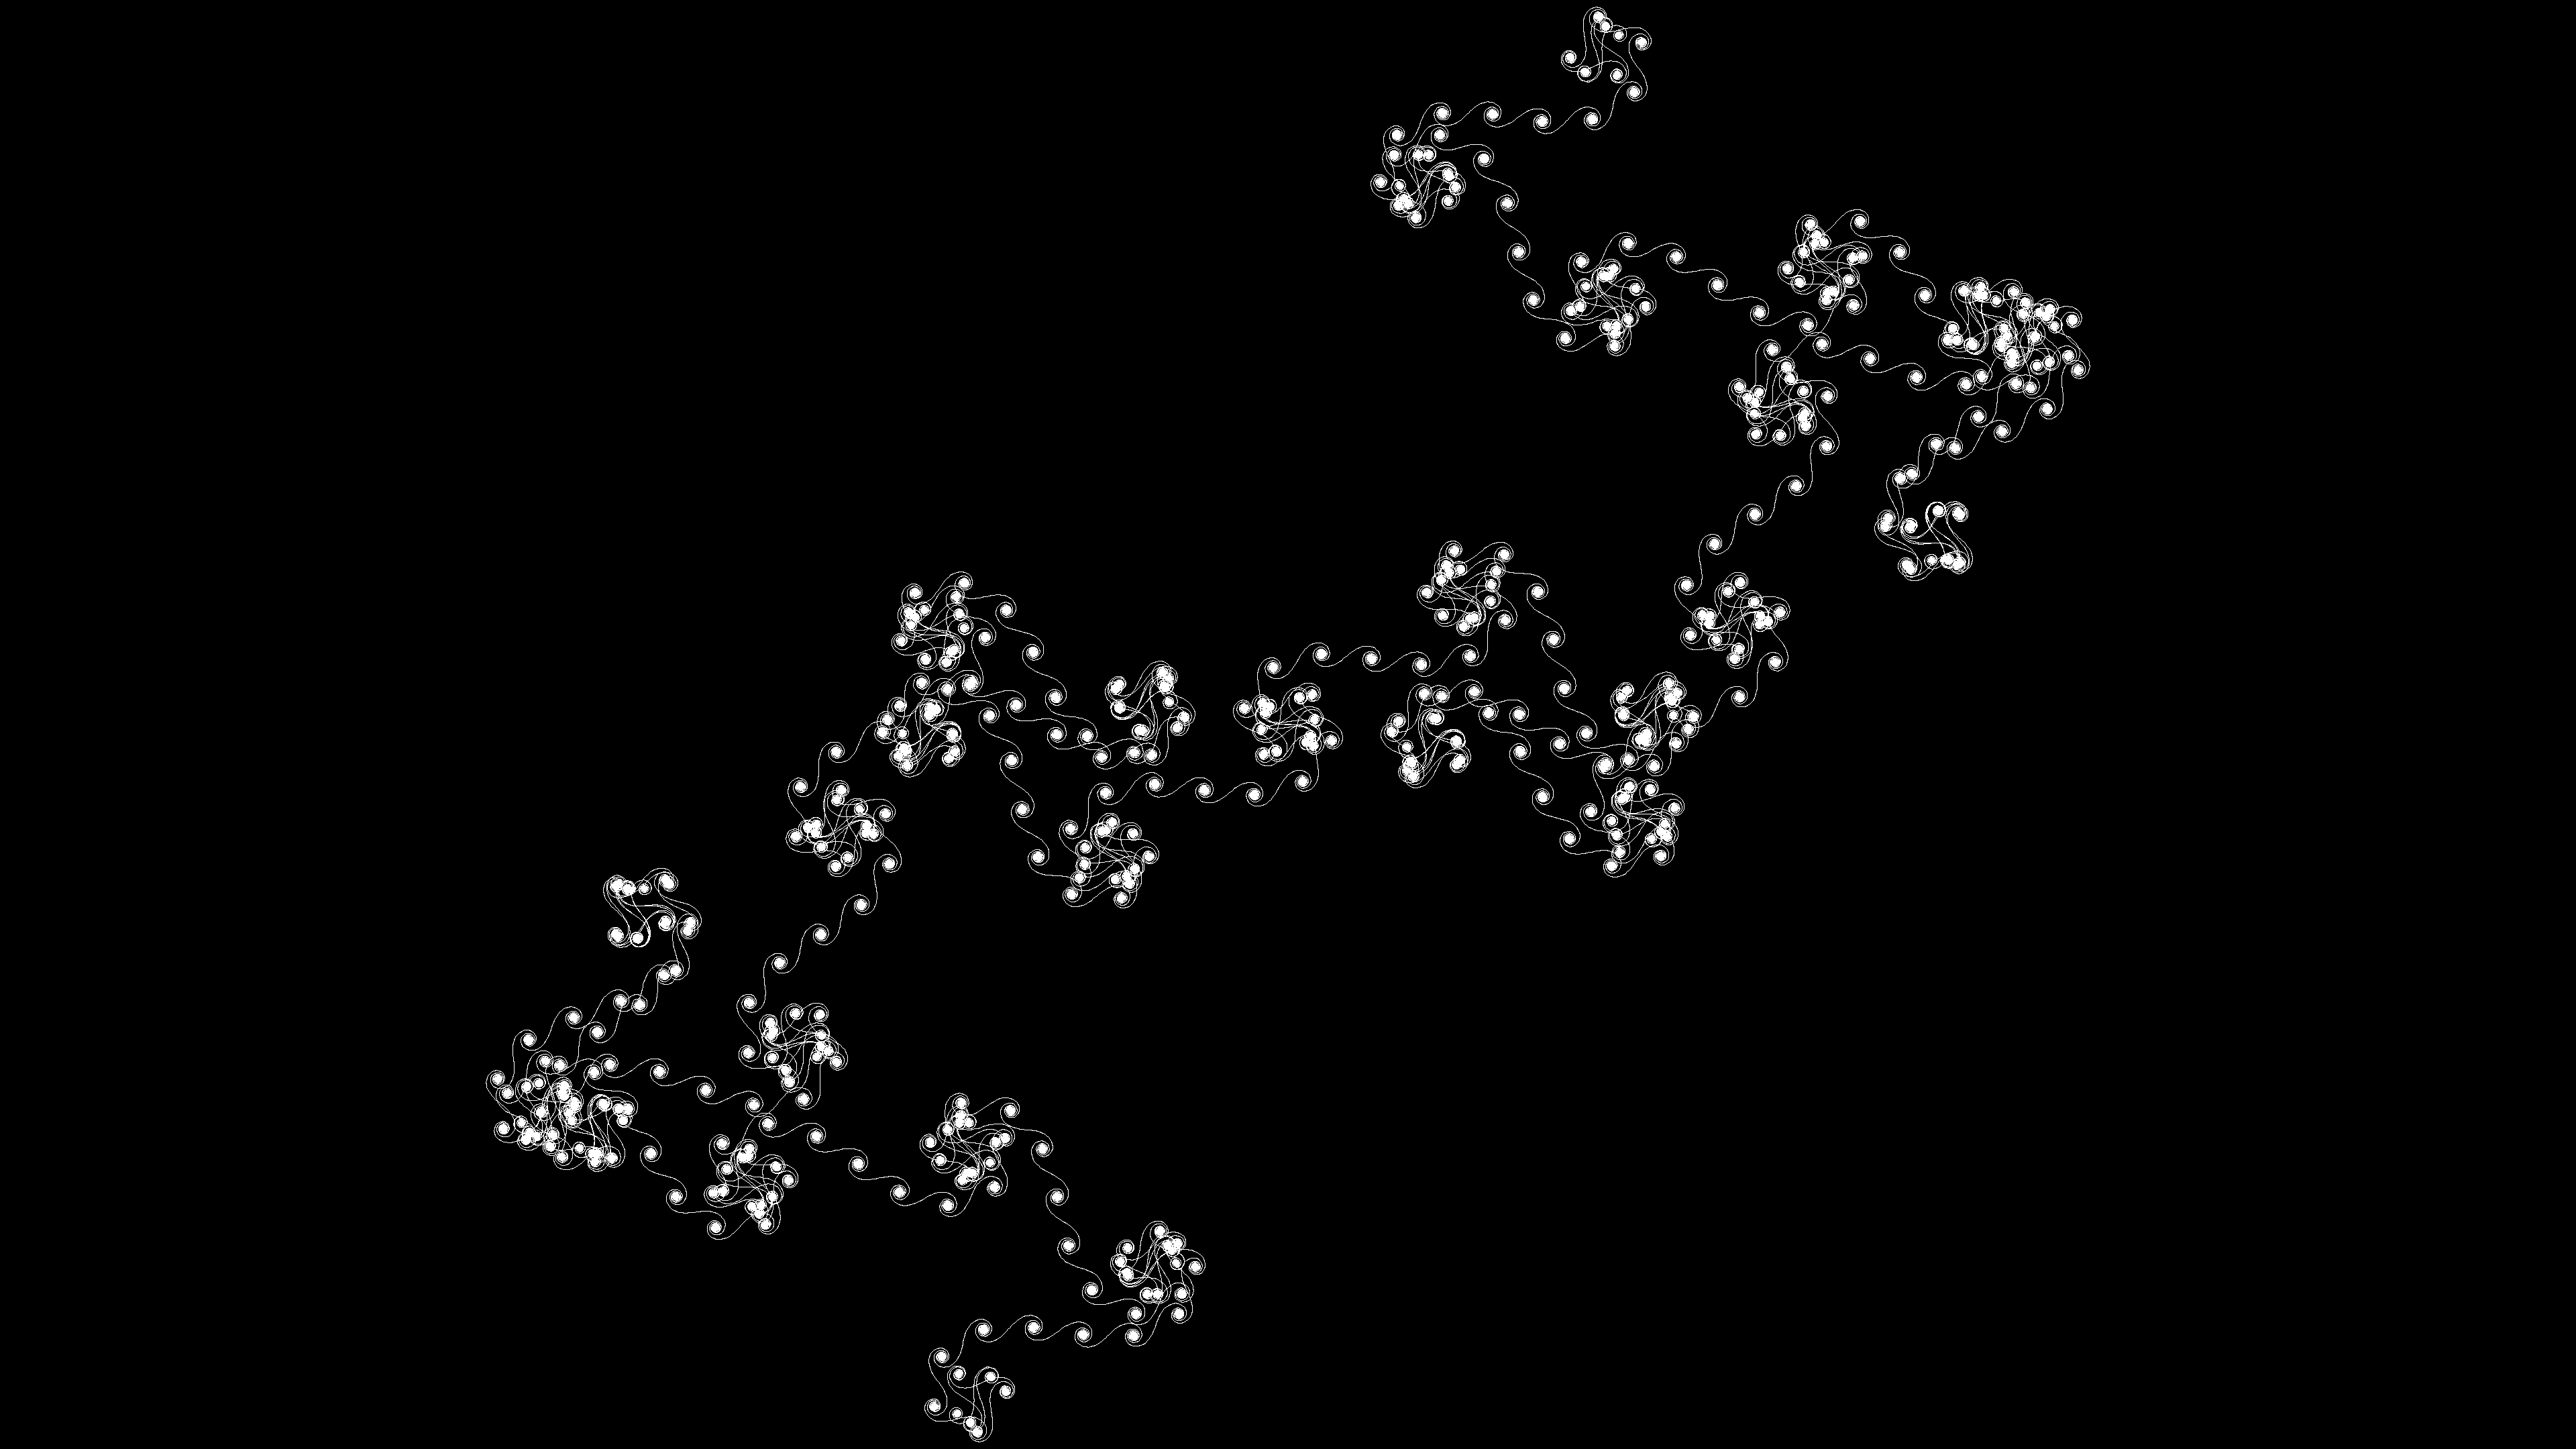
\includegraphics[width=\linewidth]{./stepsplusoneimages/0000000027.png}
    \caption{tf p=499 q=199626 theta=000 89988278.png}
  \end{subfigure}
  \begin{subfigure}[t]{0.48\textwidth}
    \centering
    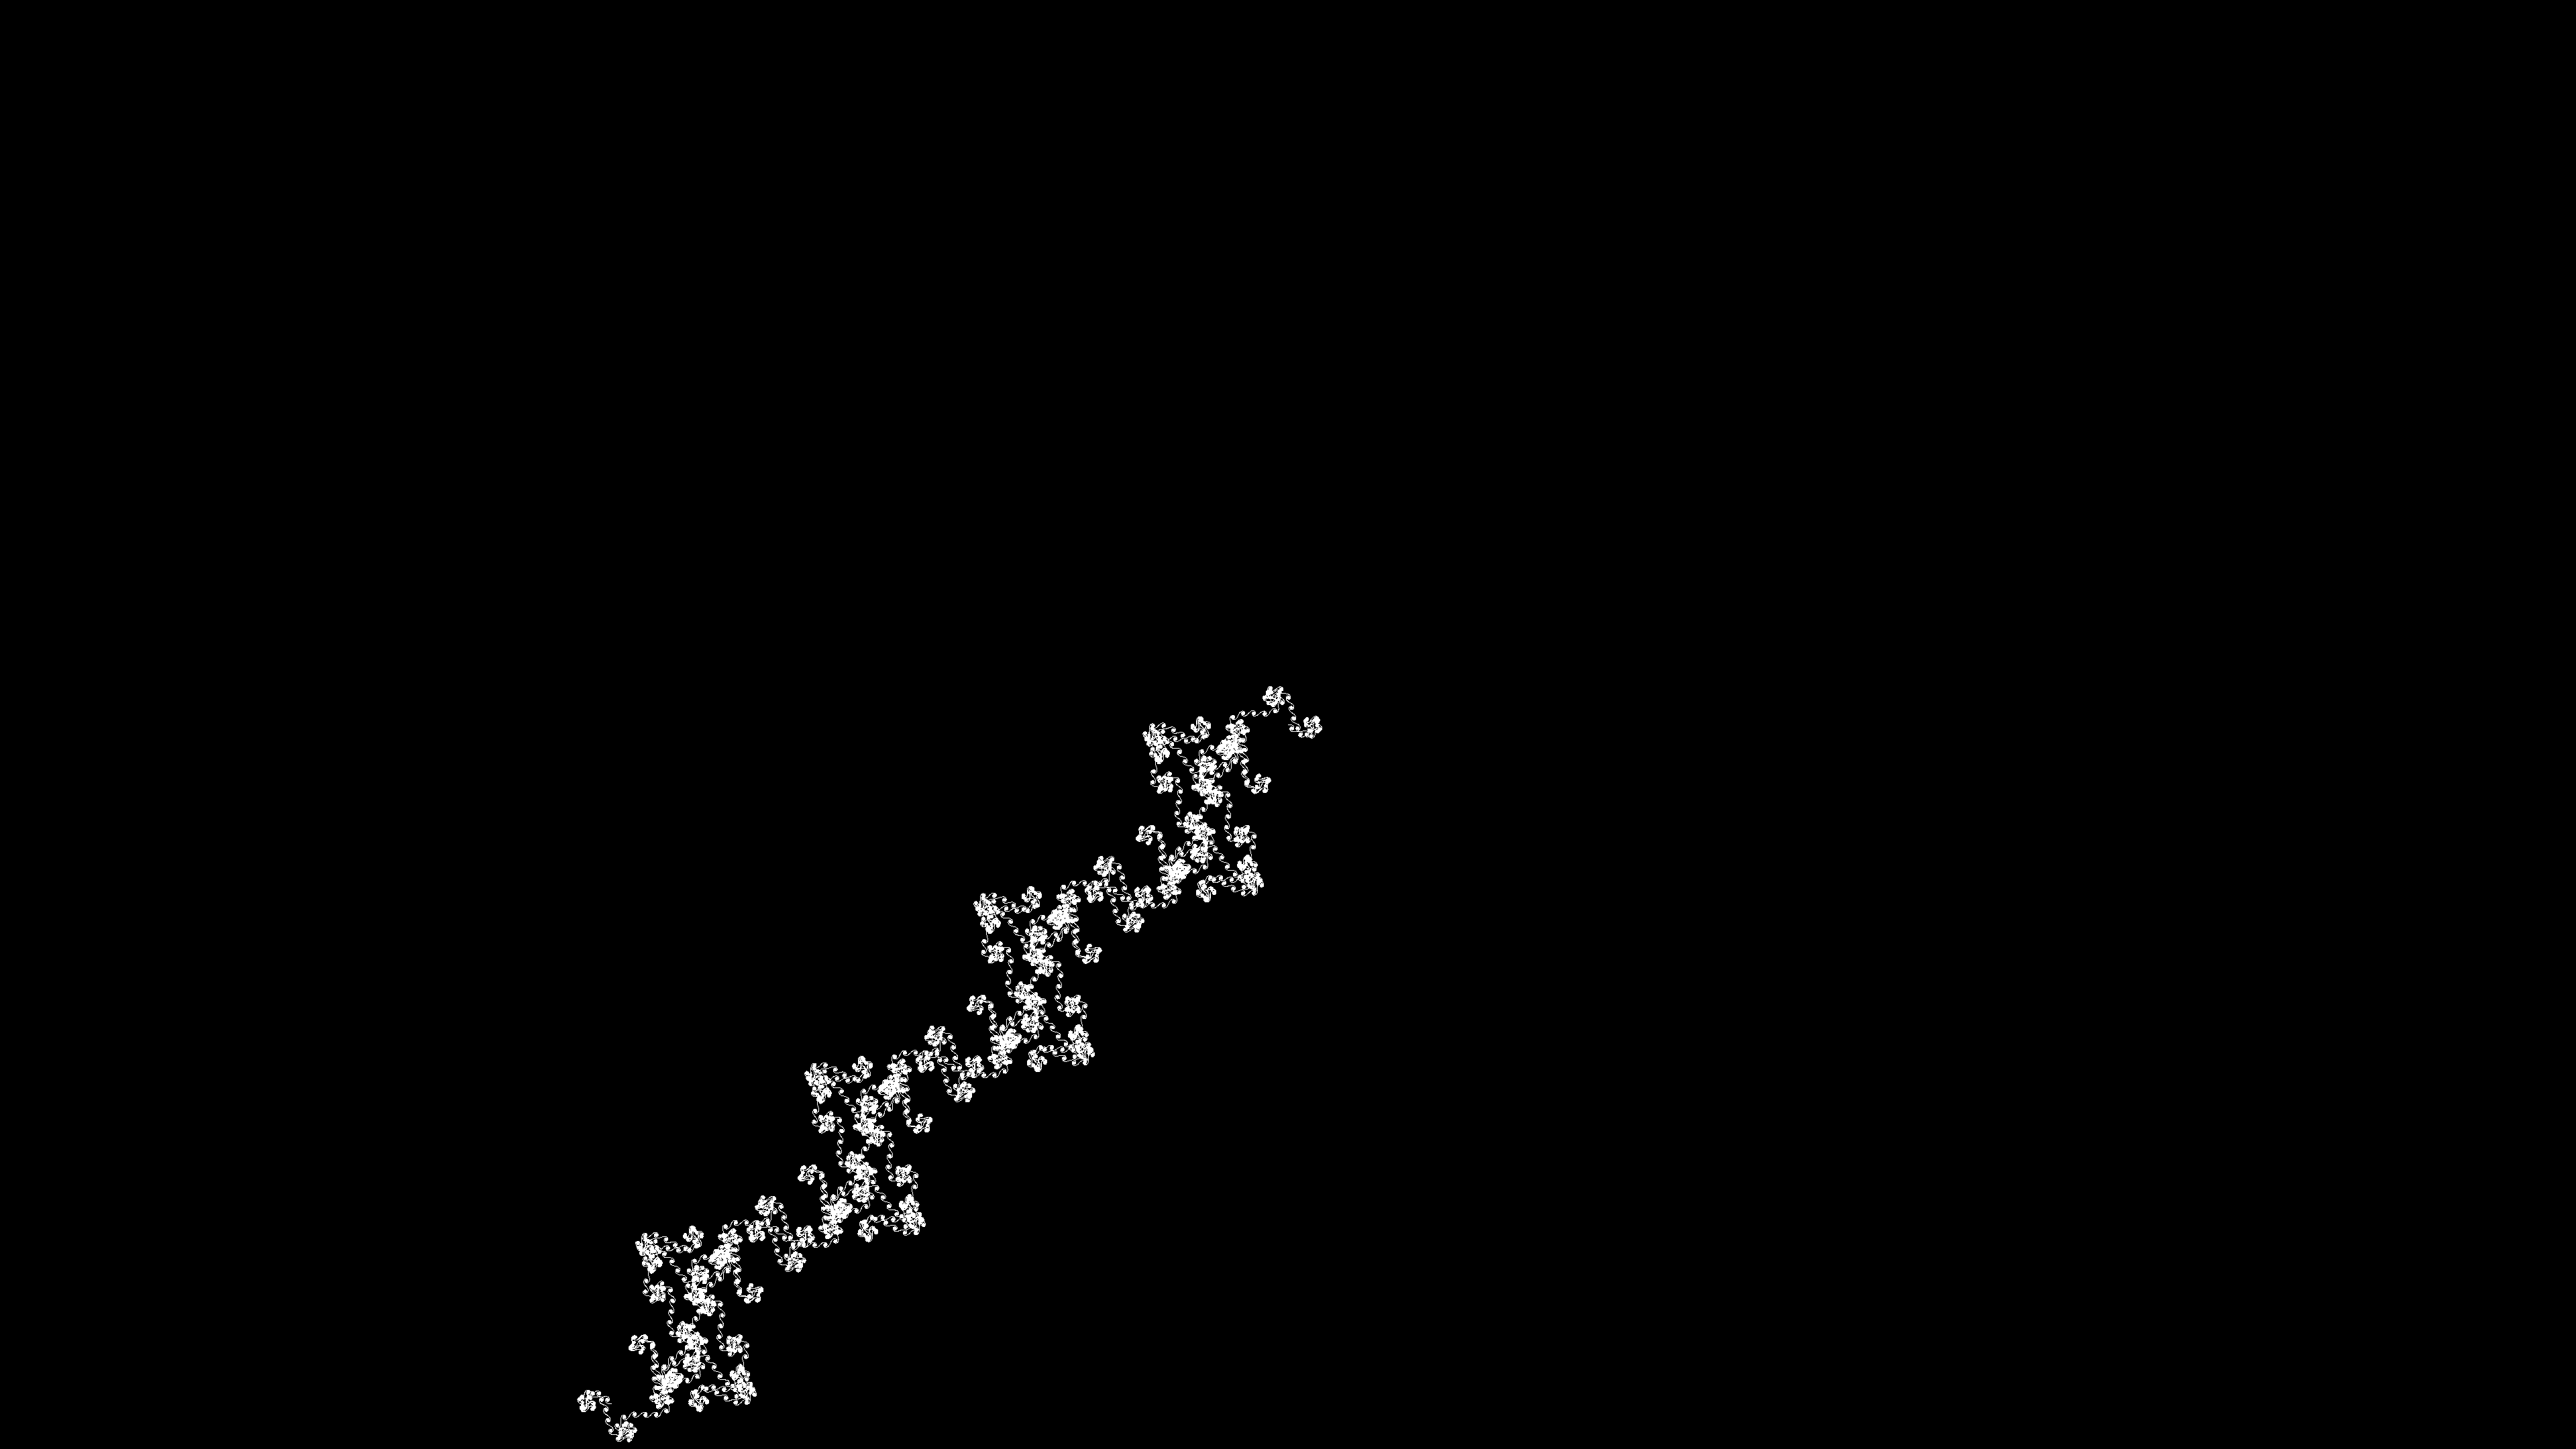
\includegraphics[width=\linewidth]{./stepsplusoneimages/0000000028.png}
    \caption{tf p=499 q=200125 theta=000 89763898.png}
  \end{subfigure}
  \caption{n=026 s=400 s+1=401}
  \label{fig:n=026}
\end{figure}
\begin{figure}[H]
  \centering
  \begin{subfigure}[t]{0.48\textwidth}
    \centering
    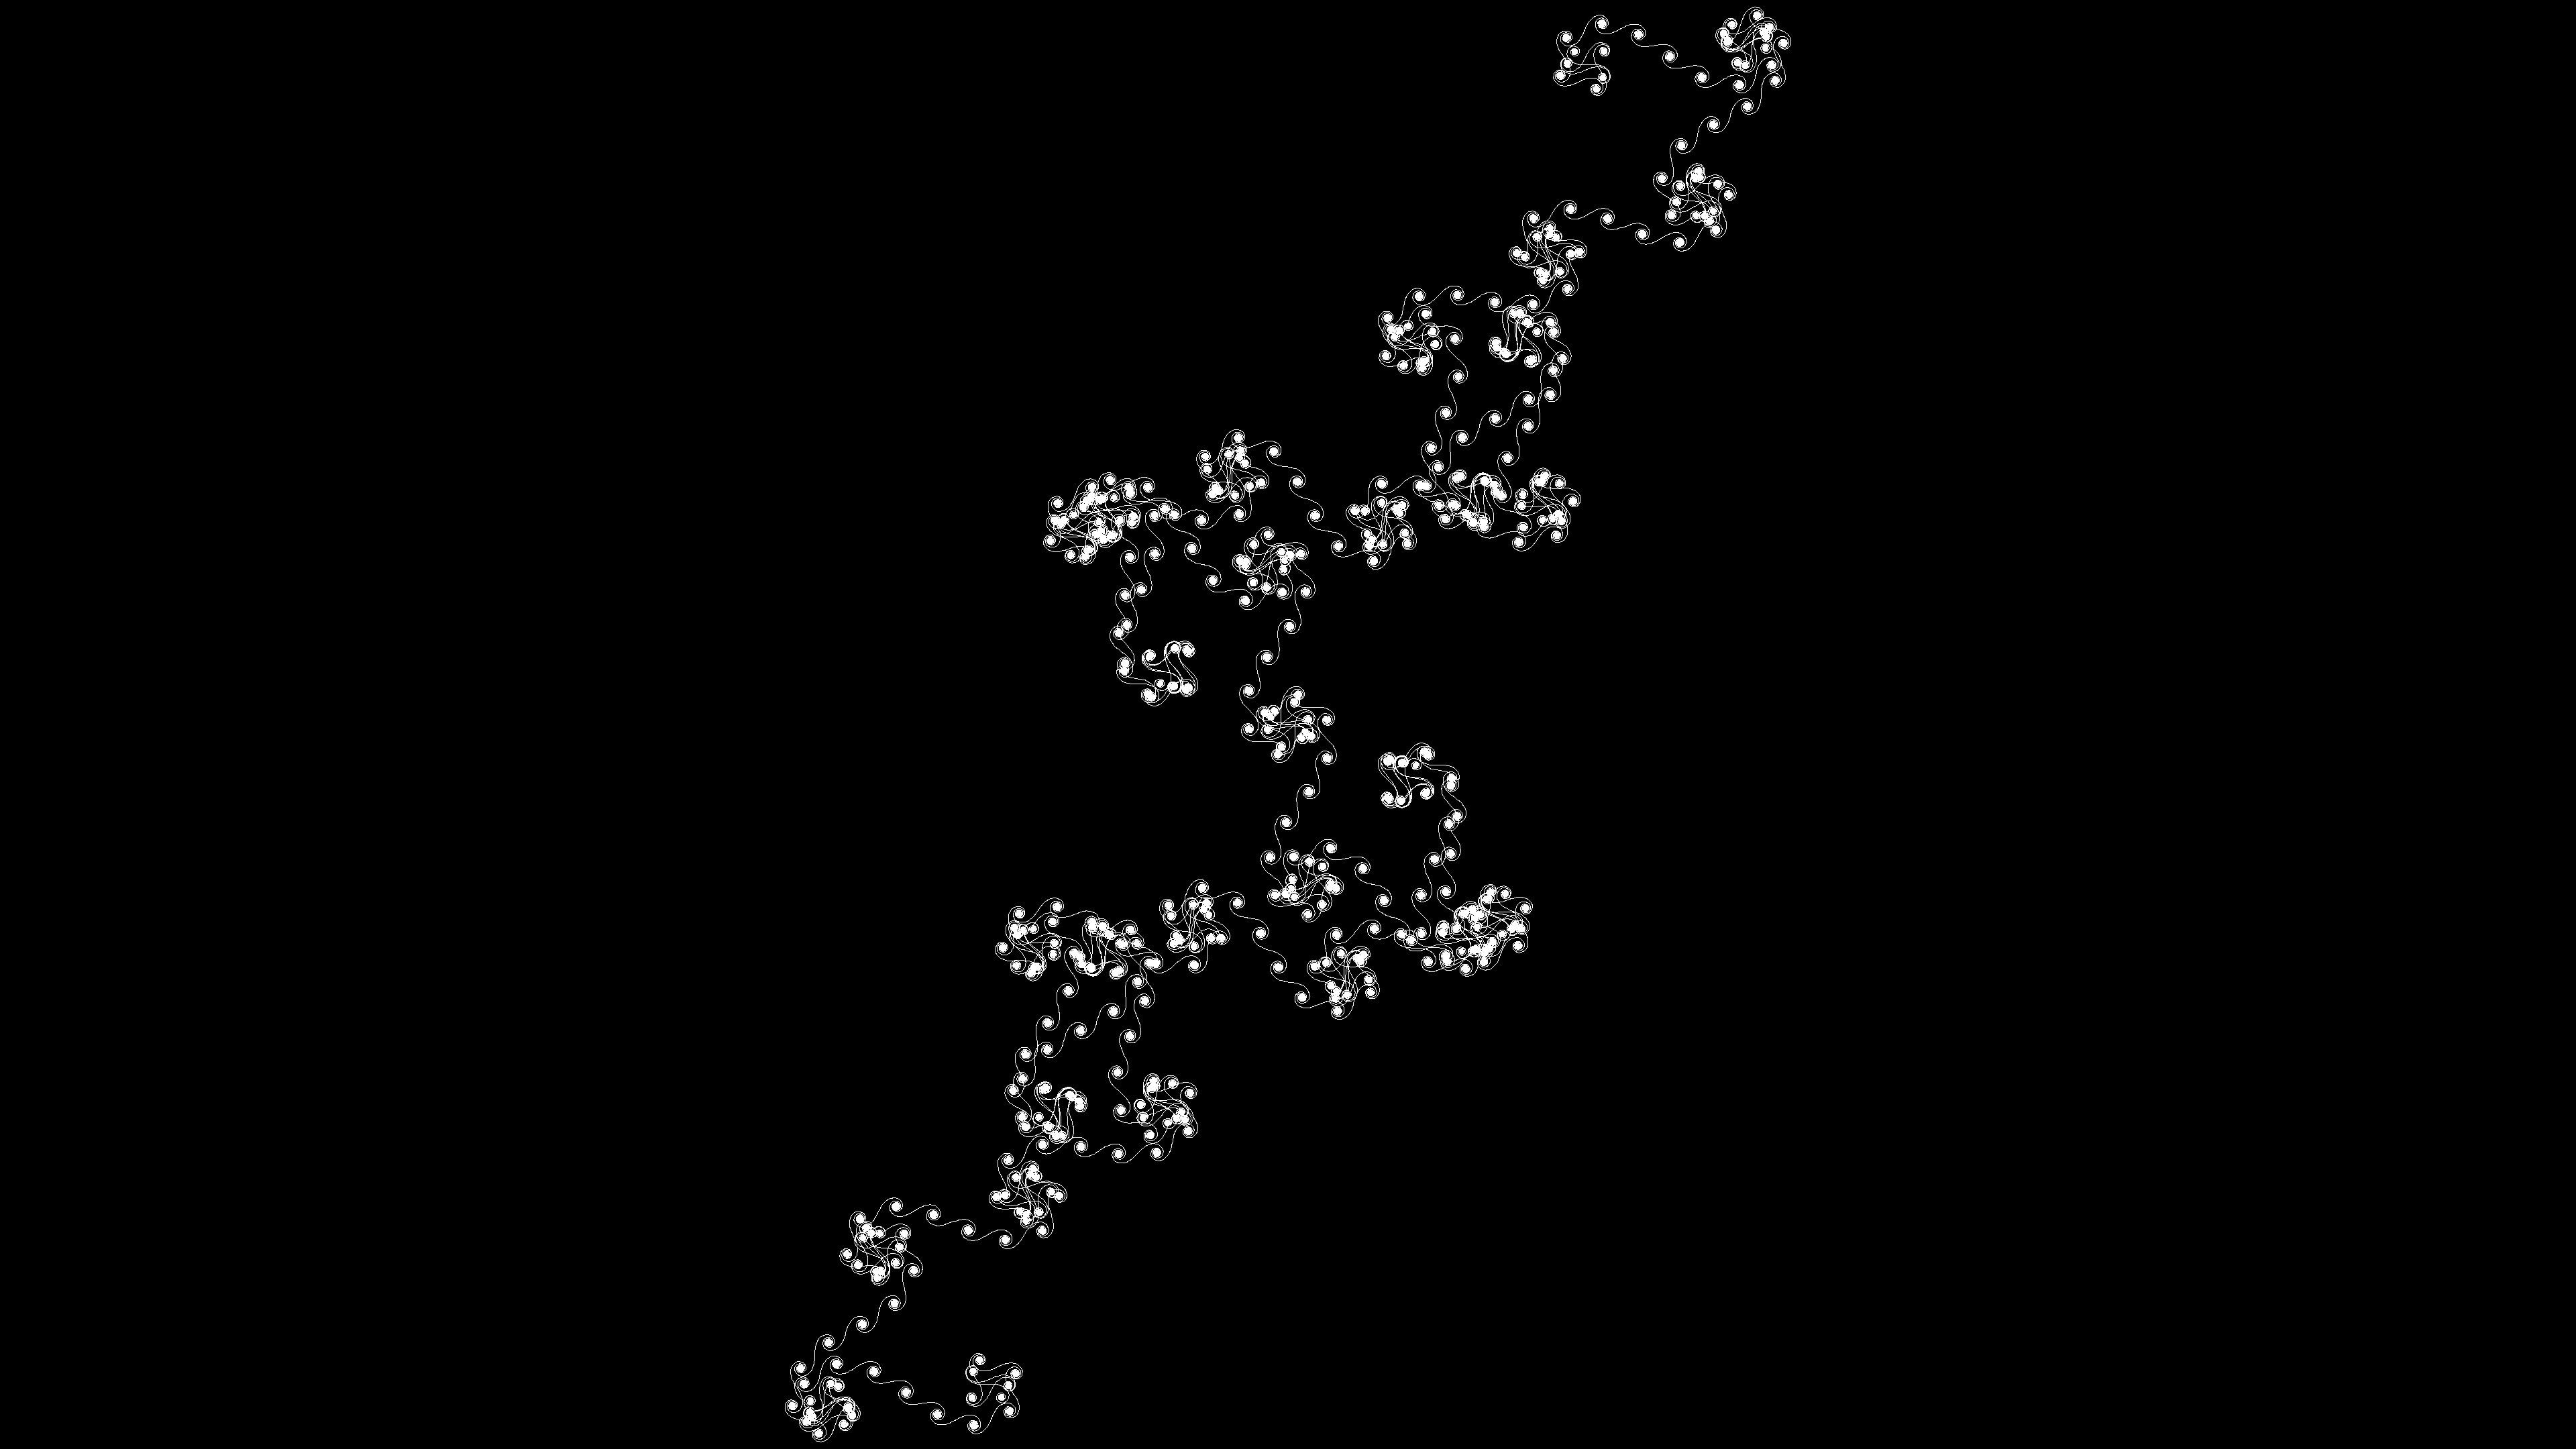
\includegraphics[width=\linewidth]{./stepsplusoneimages/0000000029.png}
    \caption{tf p=499 q=199628 theta=000 89987377.png}
  \end{subfigure}
  \begin{subfigure}[t]{0.48\textwidth}
    \centering
    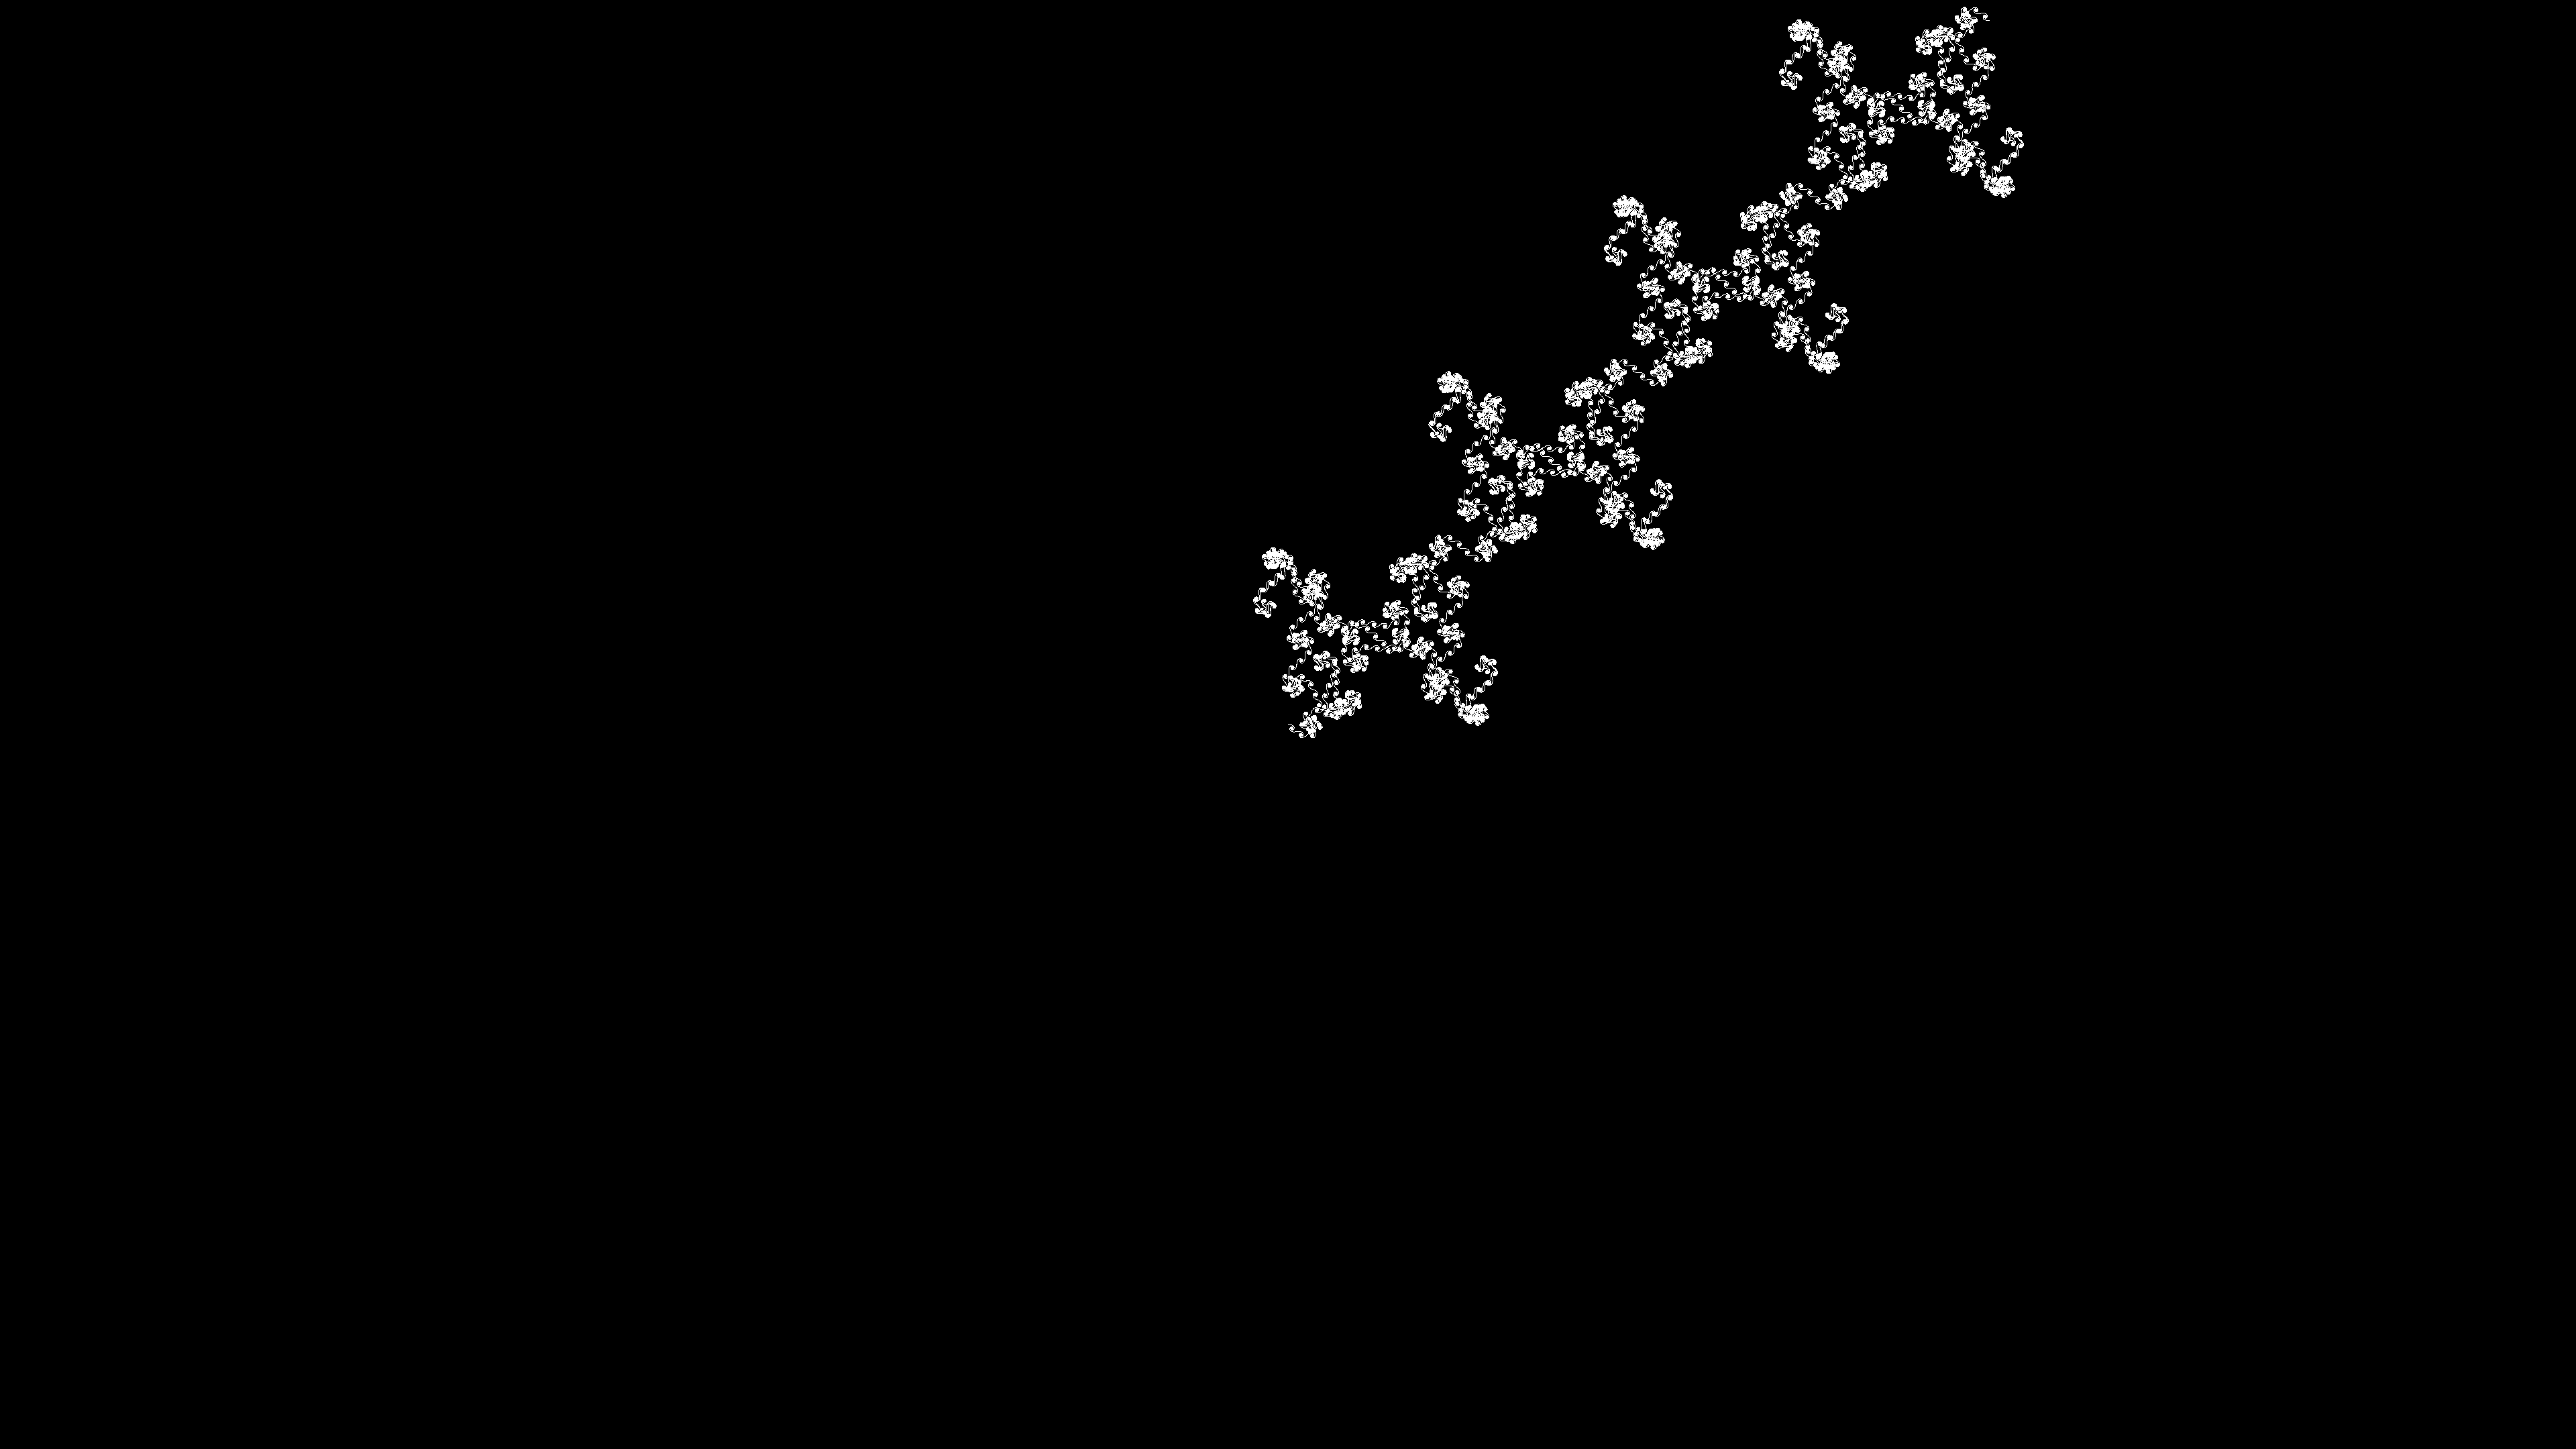
\includegraphics[width=\linewidth]{./stepsplusoneimages/0000000030.png}
    \caption{tf p=499 q=200127 theta=000 89763000.png}
  \end{subfigure}
  \caption{n=028 s=400 s+1=401}
  \label{fig:n=028}
\end{figure}
\begin{figure}[H]
  \centering
  \begin{subfigure}[t]{0.48\textwidth}
    \centering
    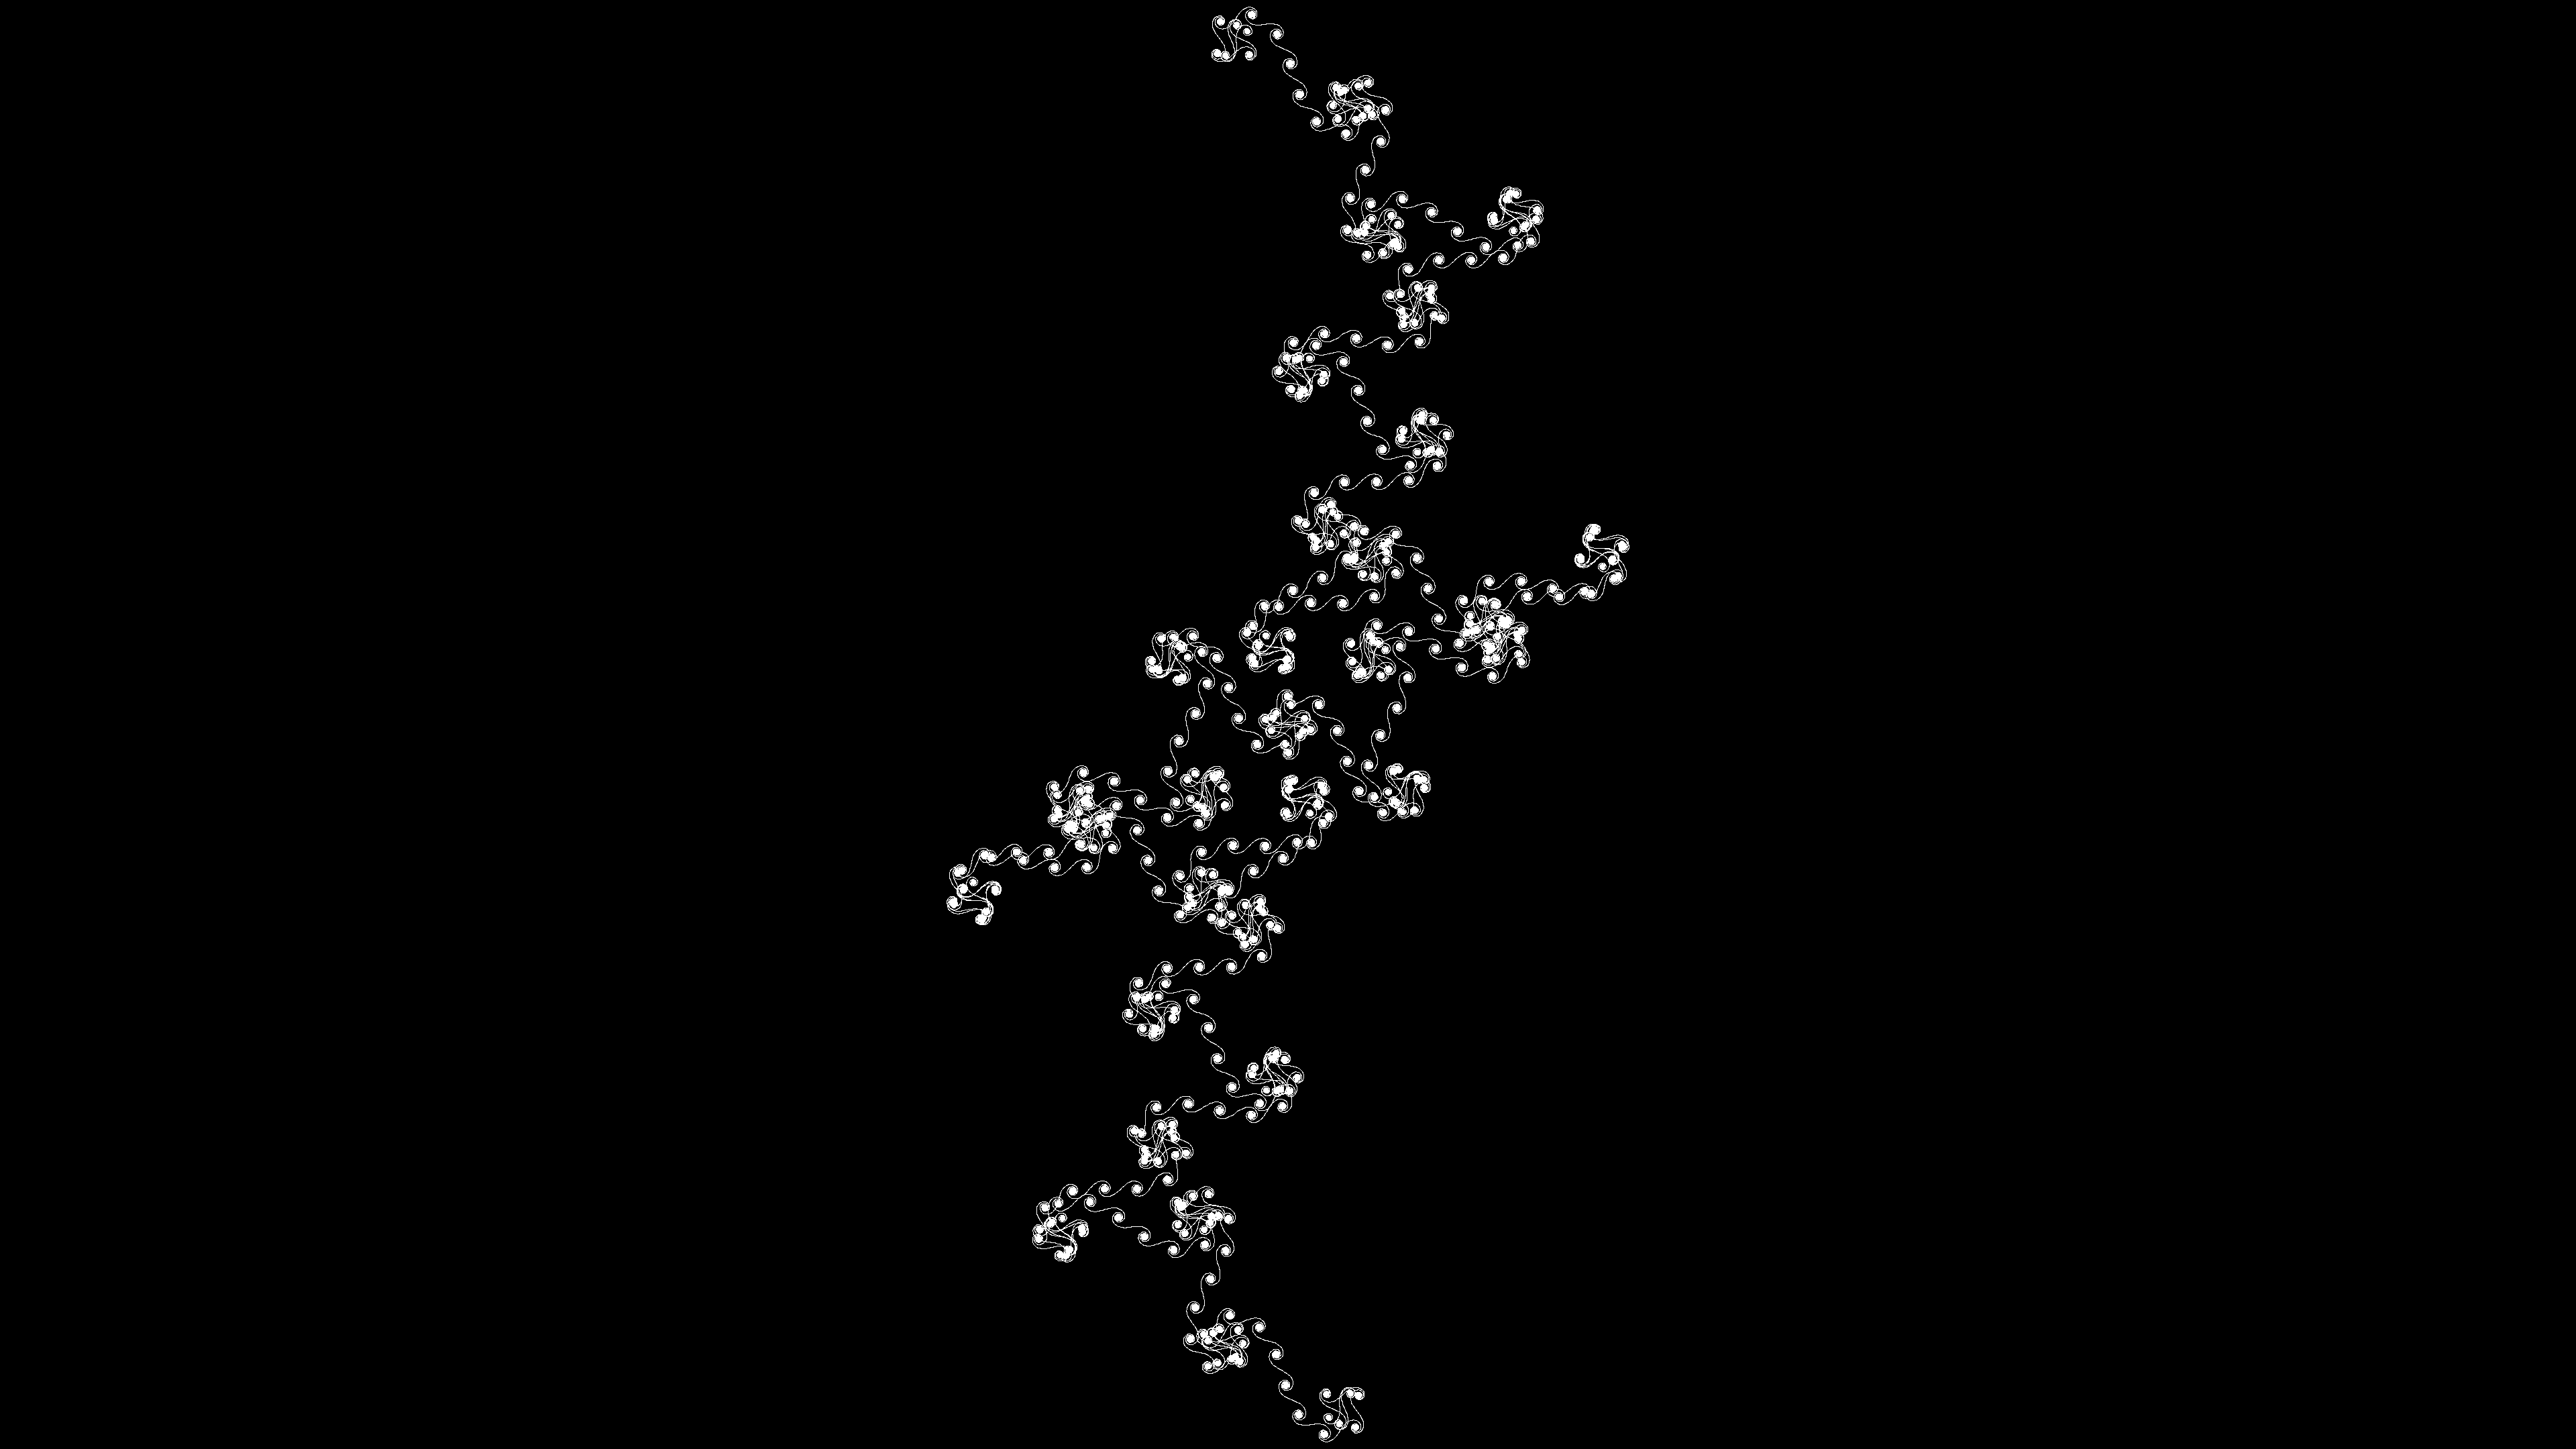
\includegraphics[width=\linewidth]{./stepsplusoneimages/0000000031.png}
    \caption{tf p=499 q=199630 theta=000 89986475.png}
  \end{subfigure}
  \begin{subfigure}[t]{0.48\textwidth}
    \centering
    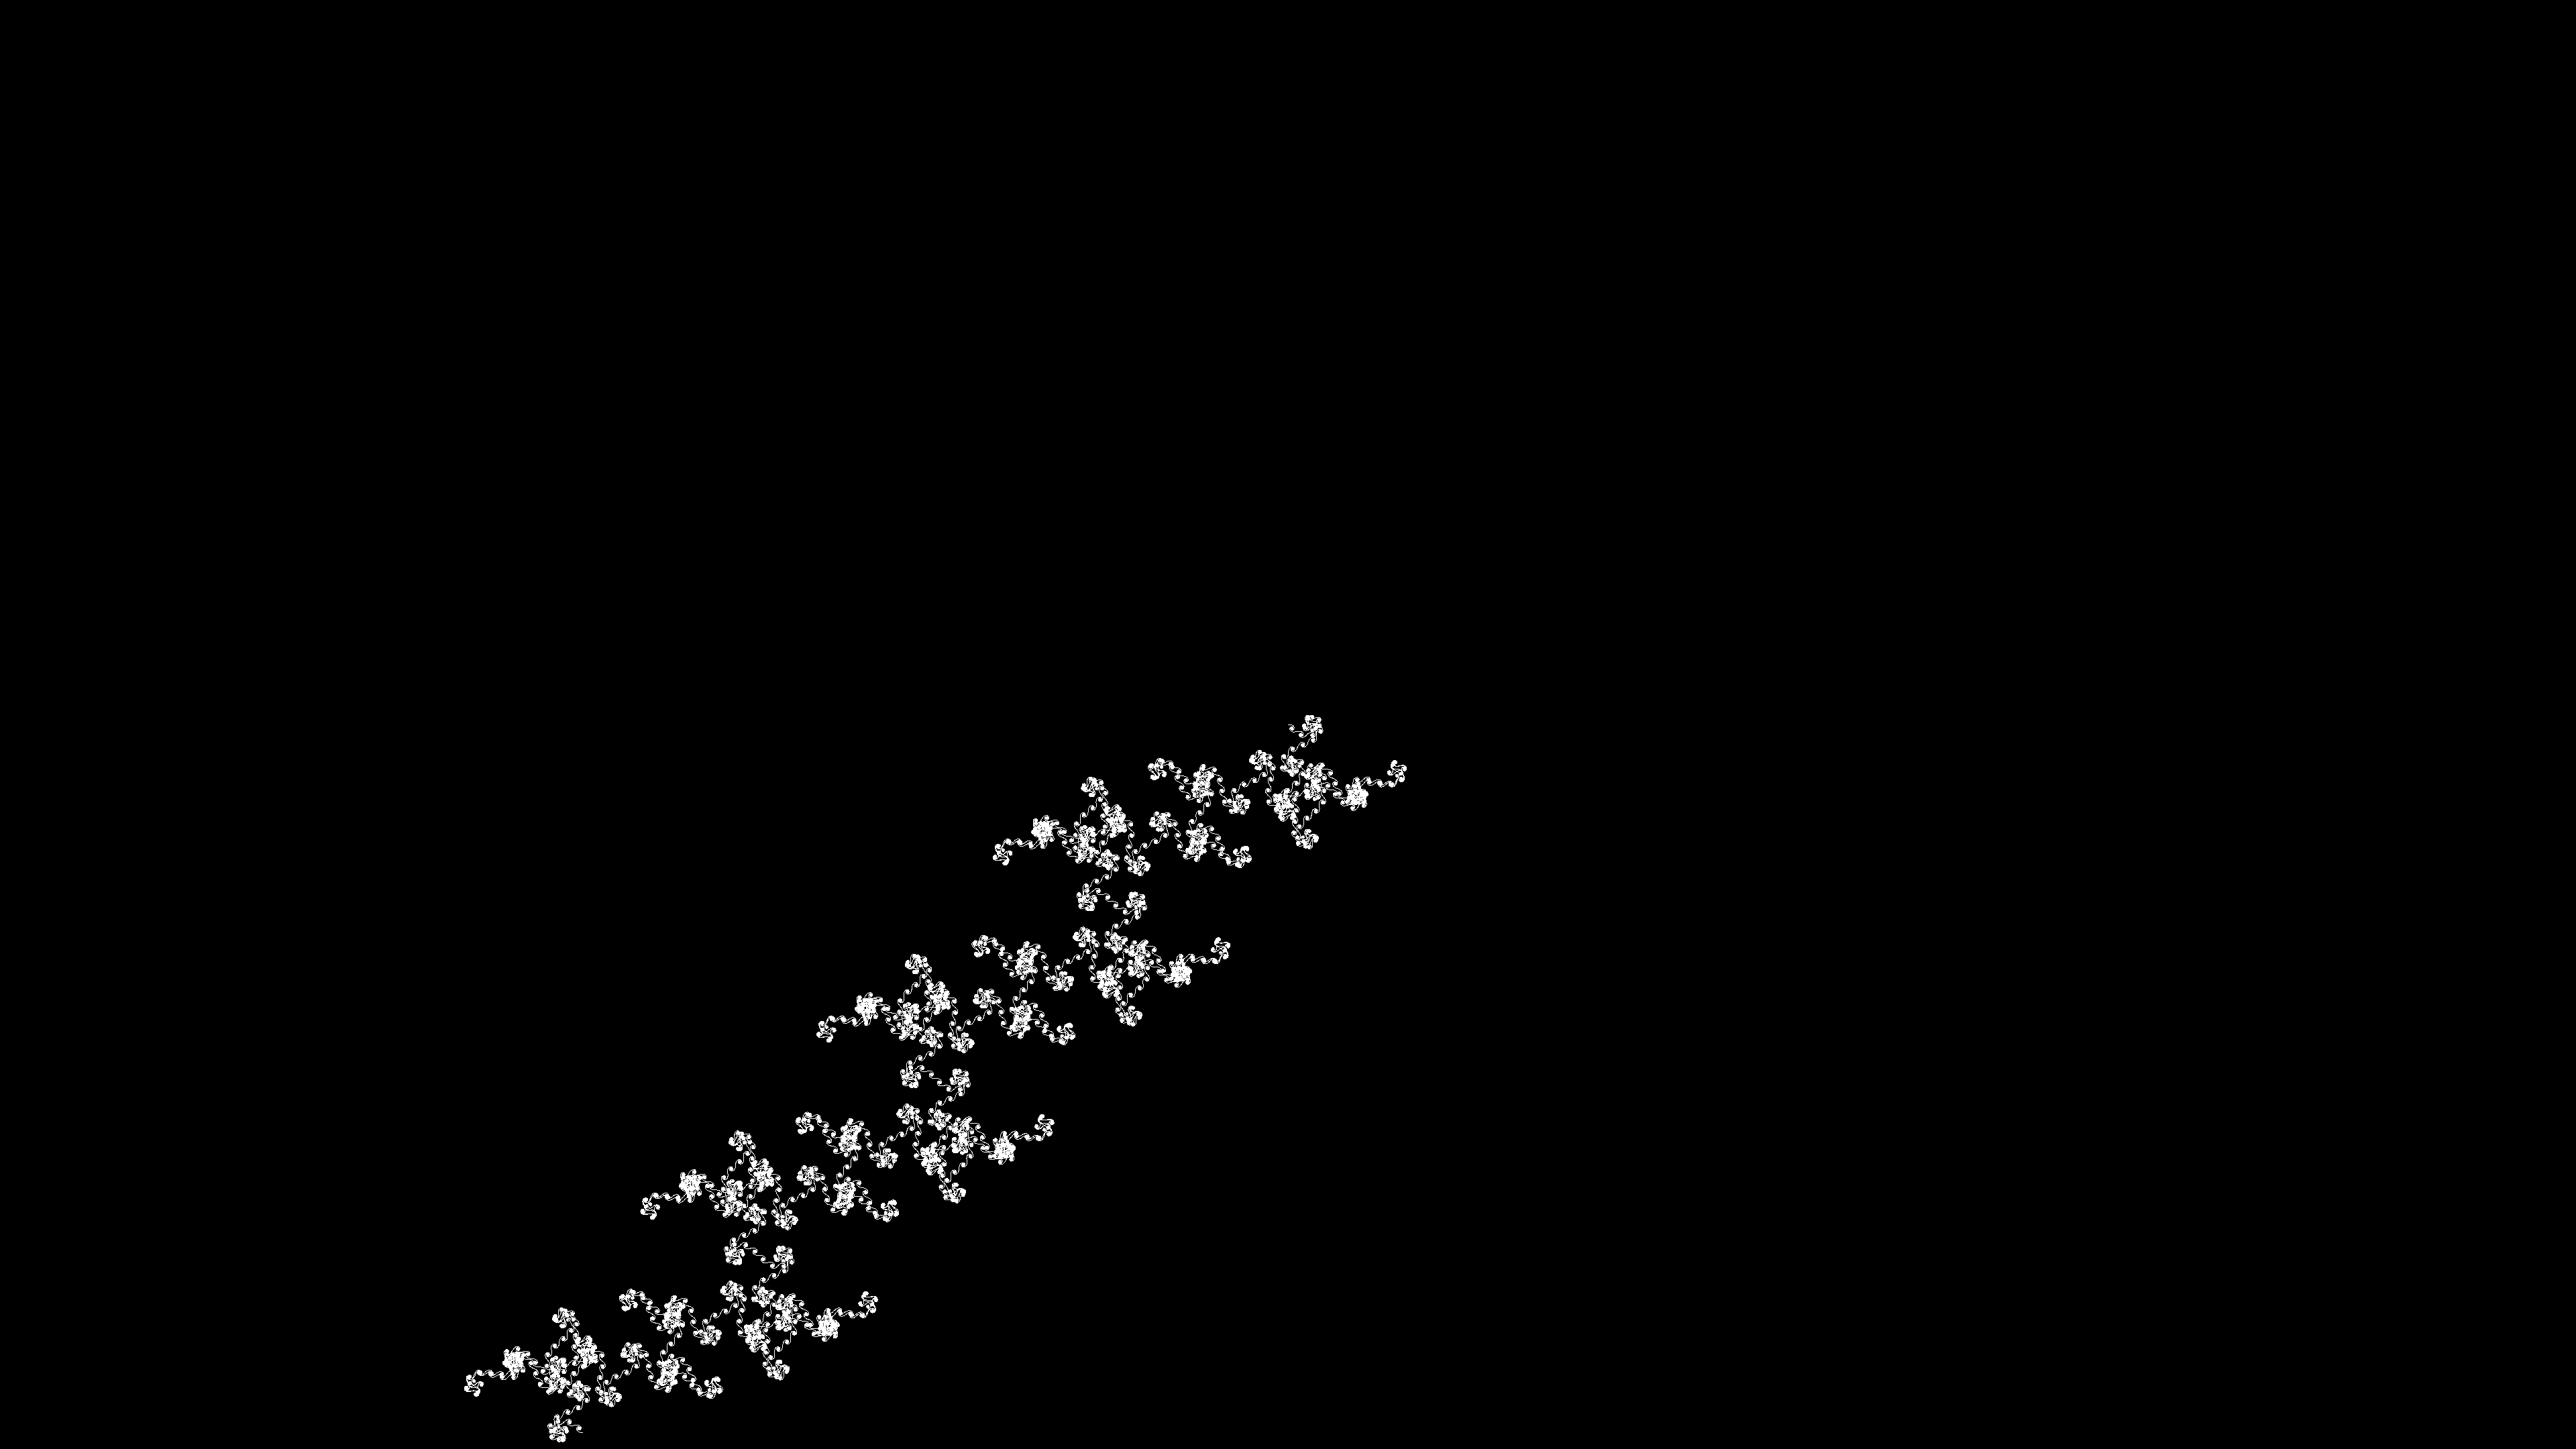
\includegraphics[width=\linewidth]{./stepsplusoneimages/0000000032.png}
    \caption{tf p=499 q=200129 theta=000 89762103.png}
  \end{subfigure}
  \caption{n=030 s=400 s+1=401}
  \label{fig:n=030}
\end{figure}
\begin{figure}[H]
  \centering
  \begin{subfigure}[t]{0.48\textwidth}
    \centering
    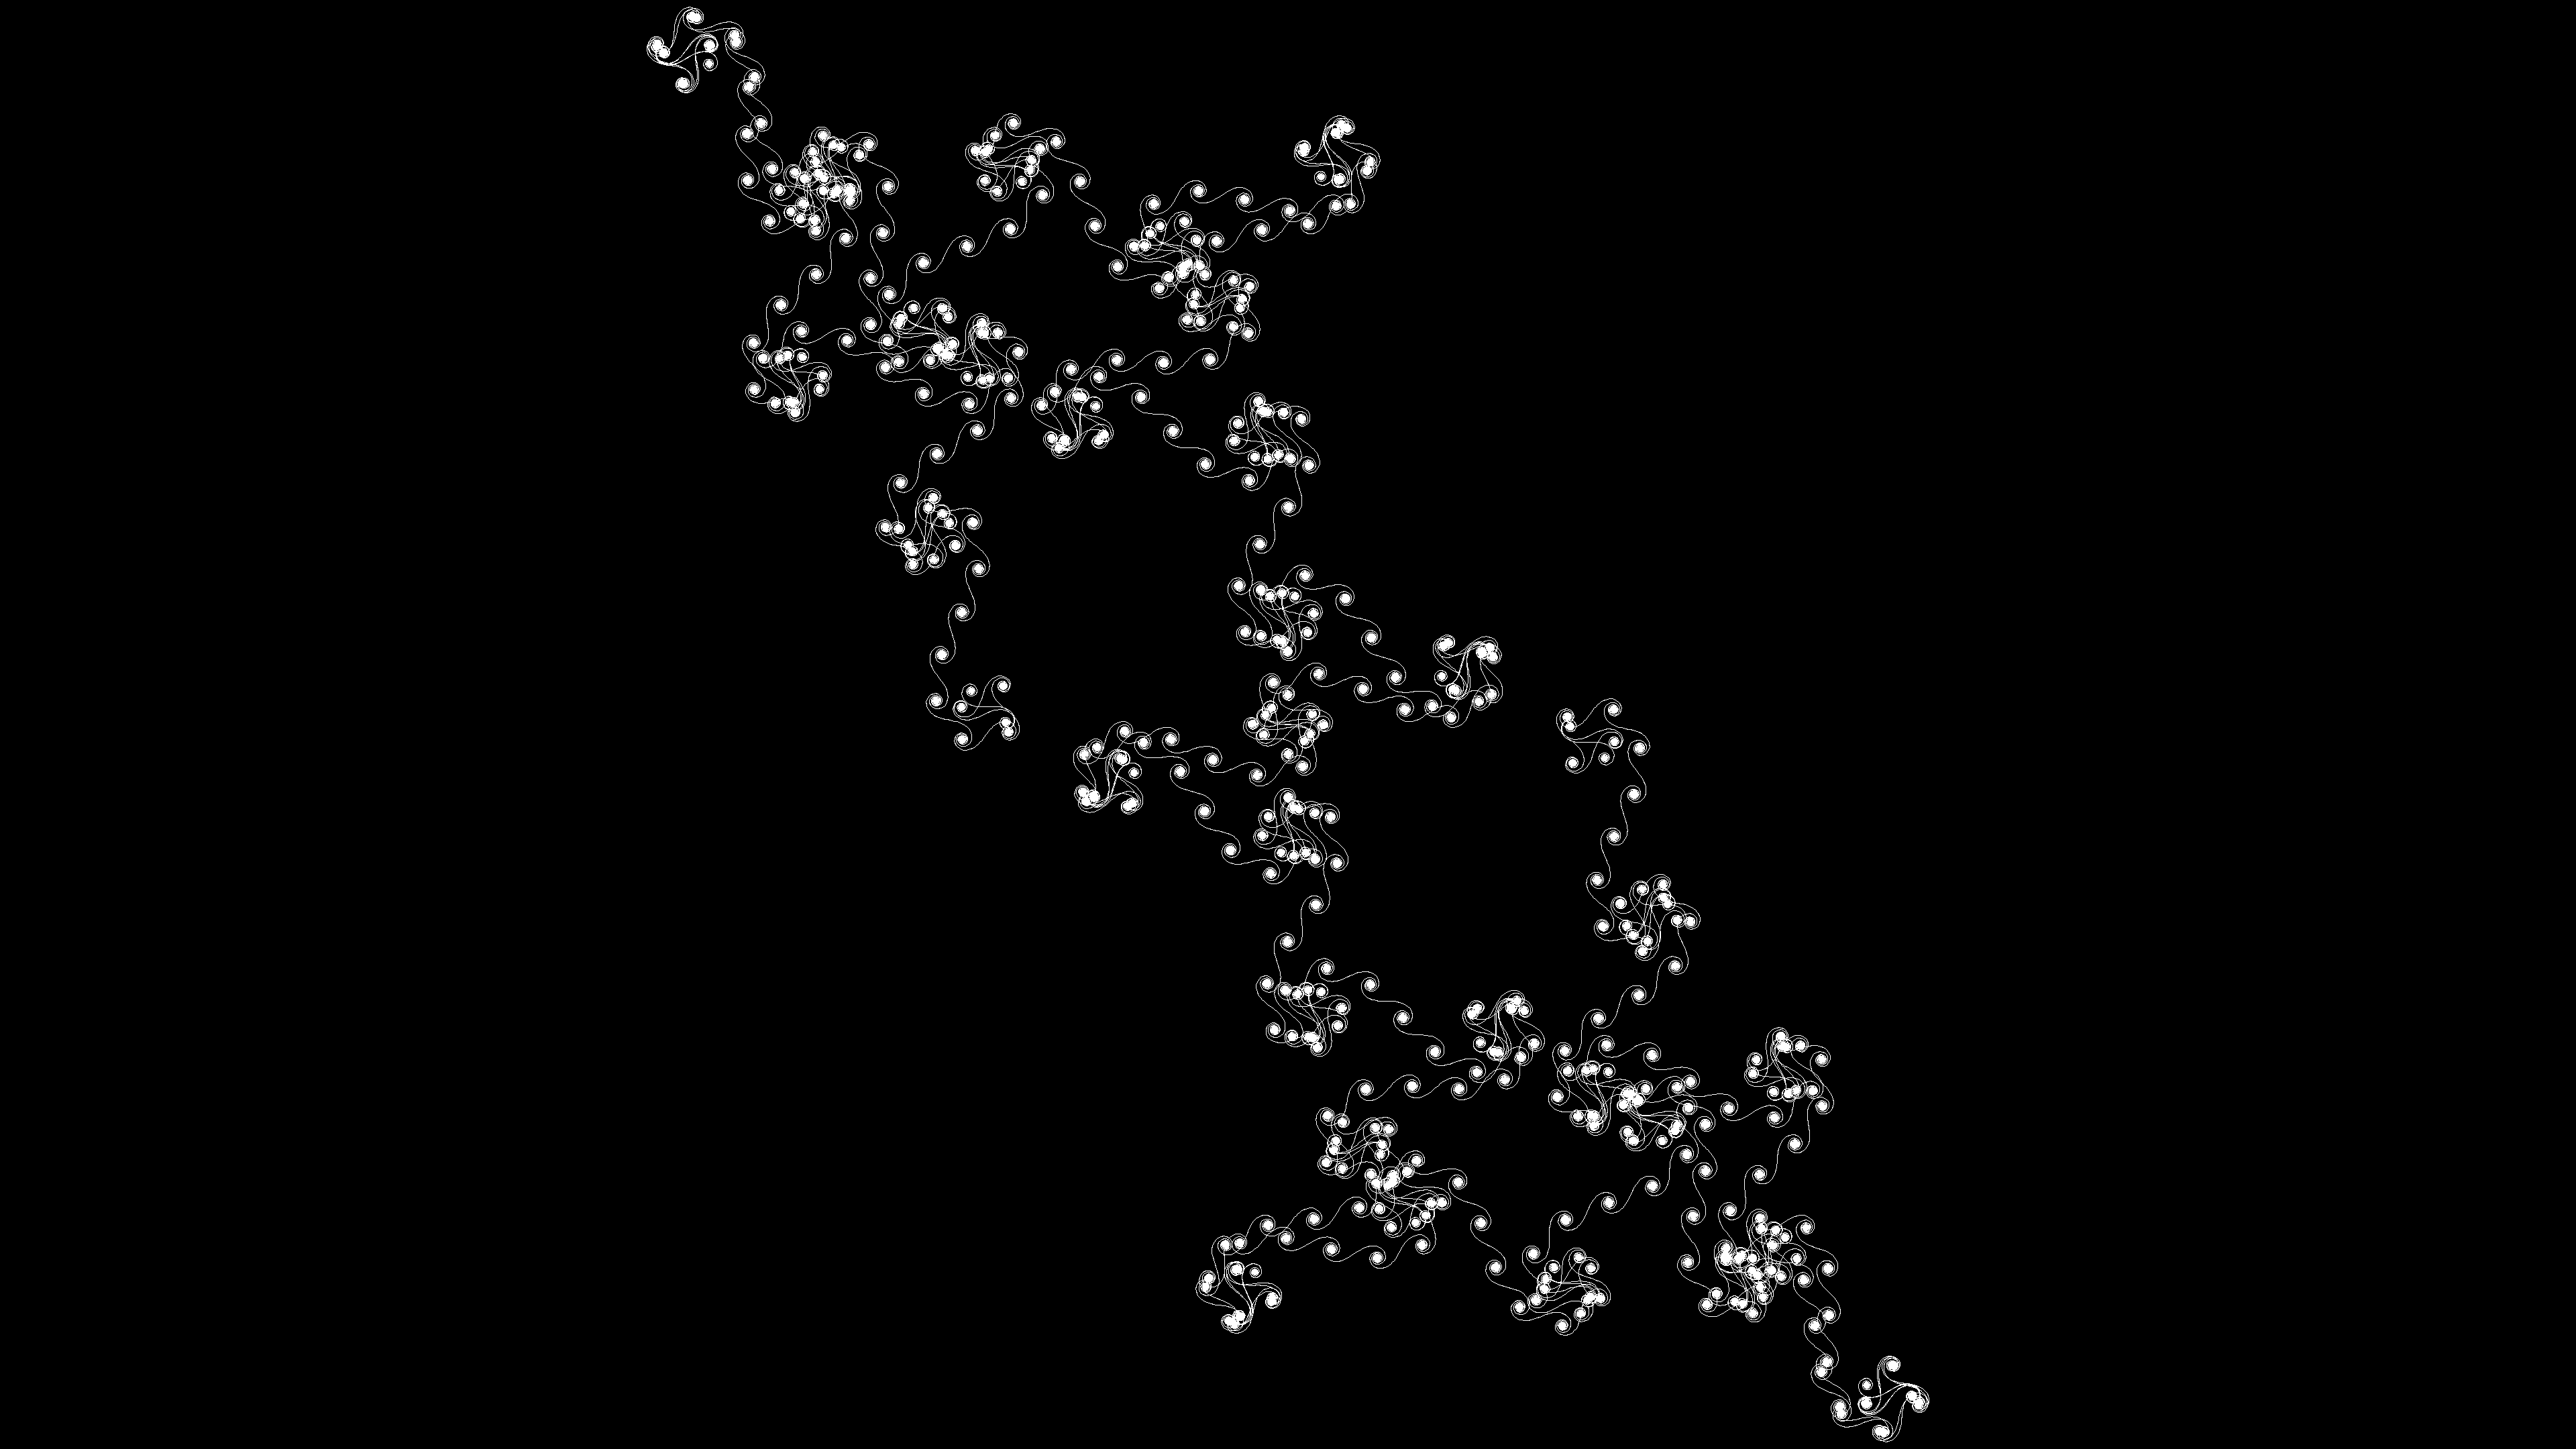
\includegraphics[width=\linewidth]{./stepsplusoneimages/0000000033.png}
    \caption{tf p=499 q=199632 theta=000 89985573.png}
  \end{subfigure}
  \begin{subfigure}[t]{0.48\textwidth}
    \centering
    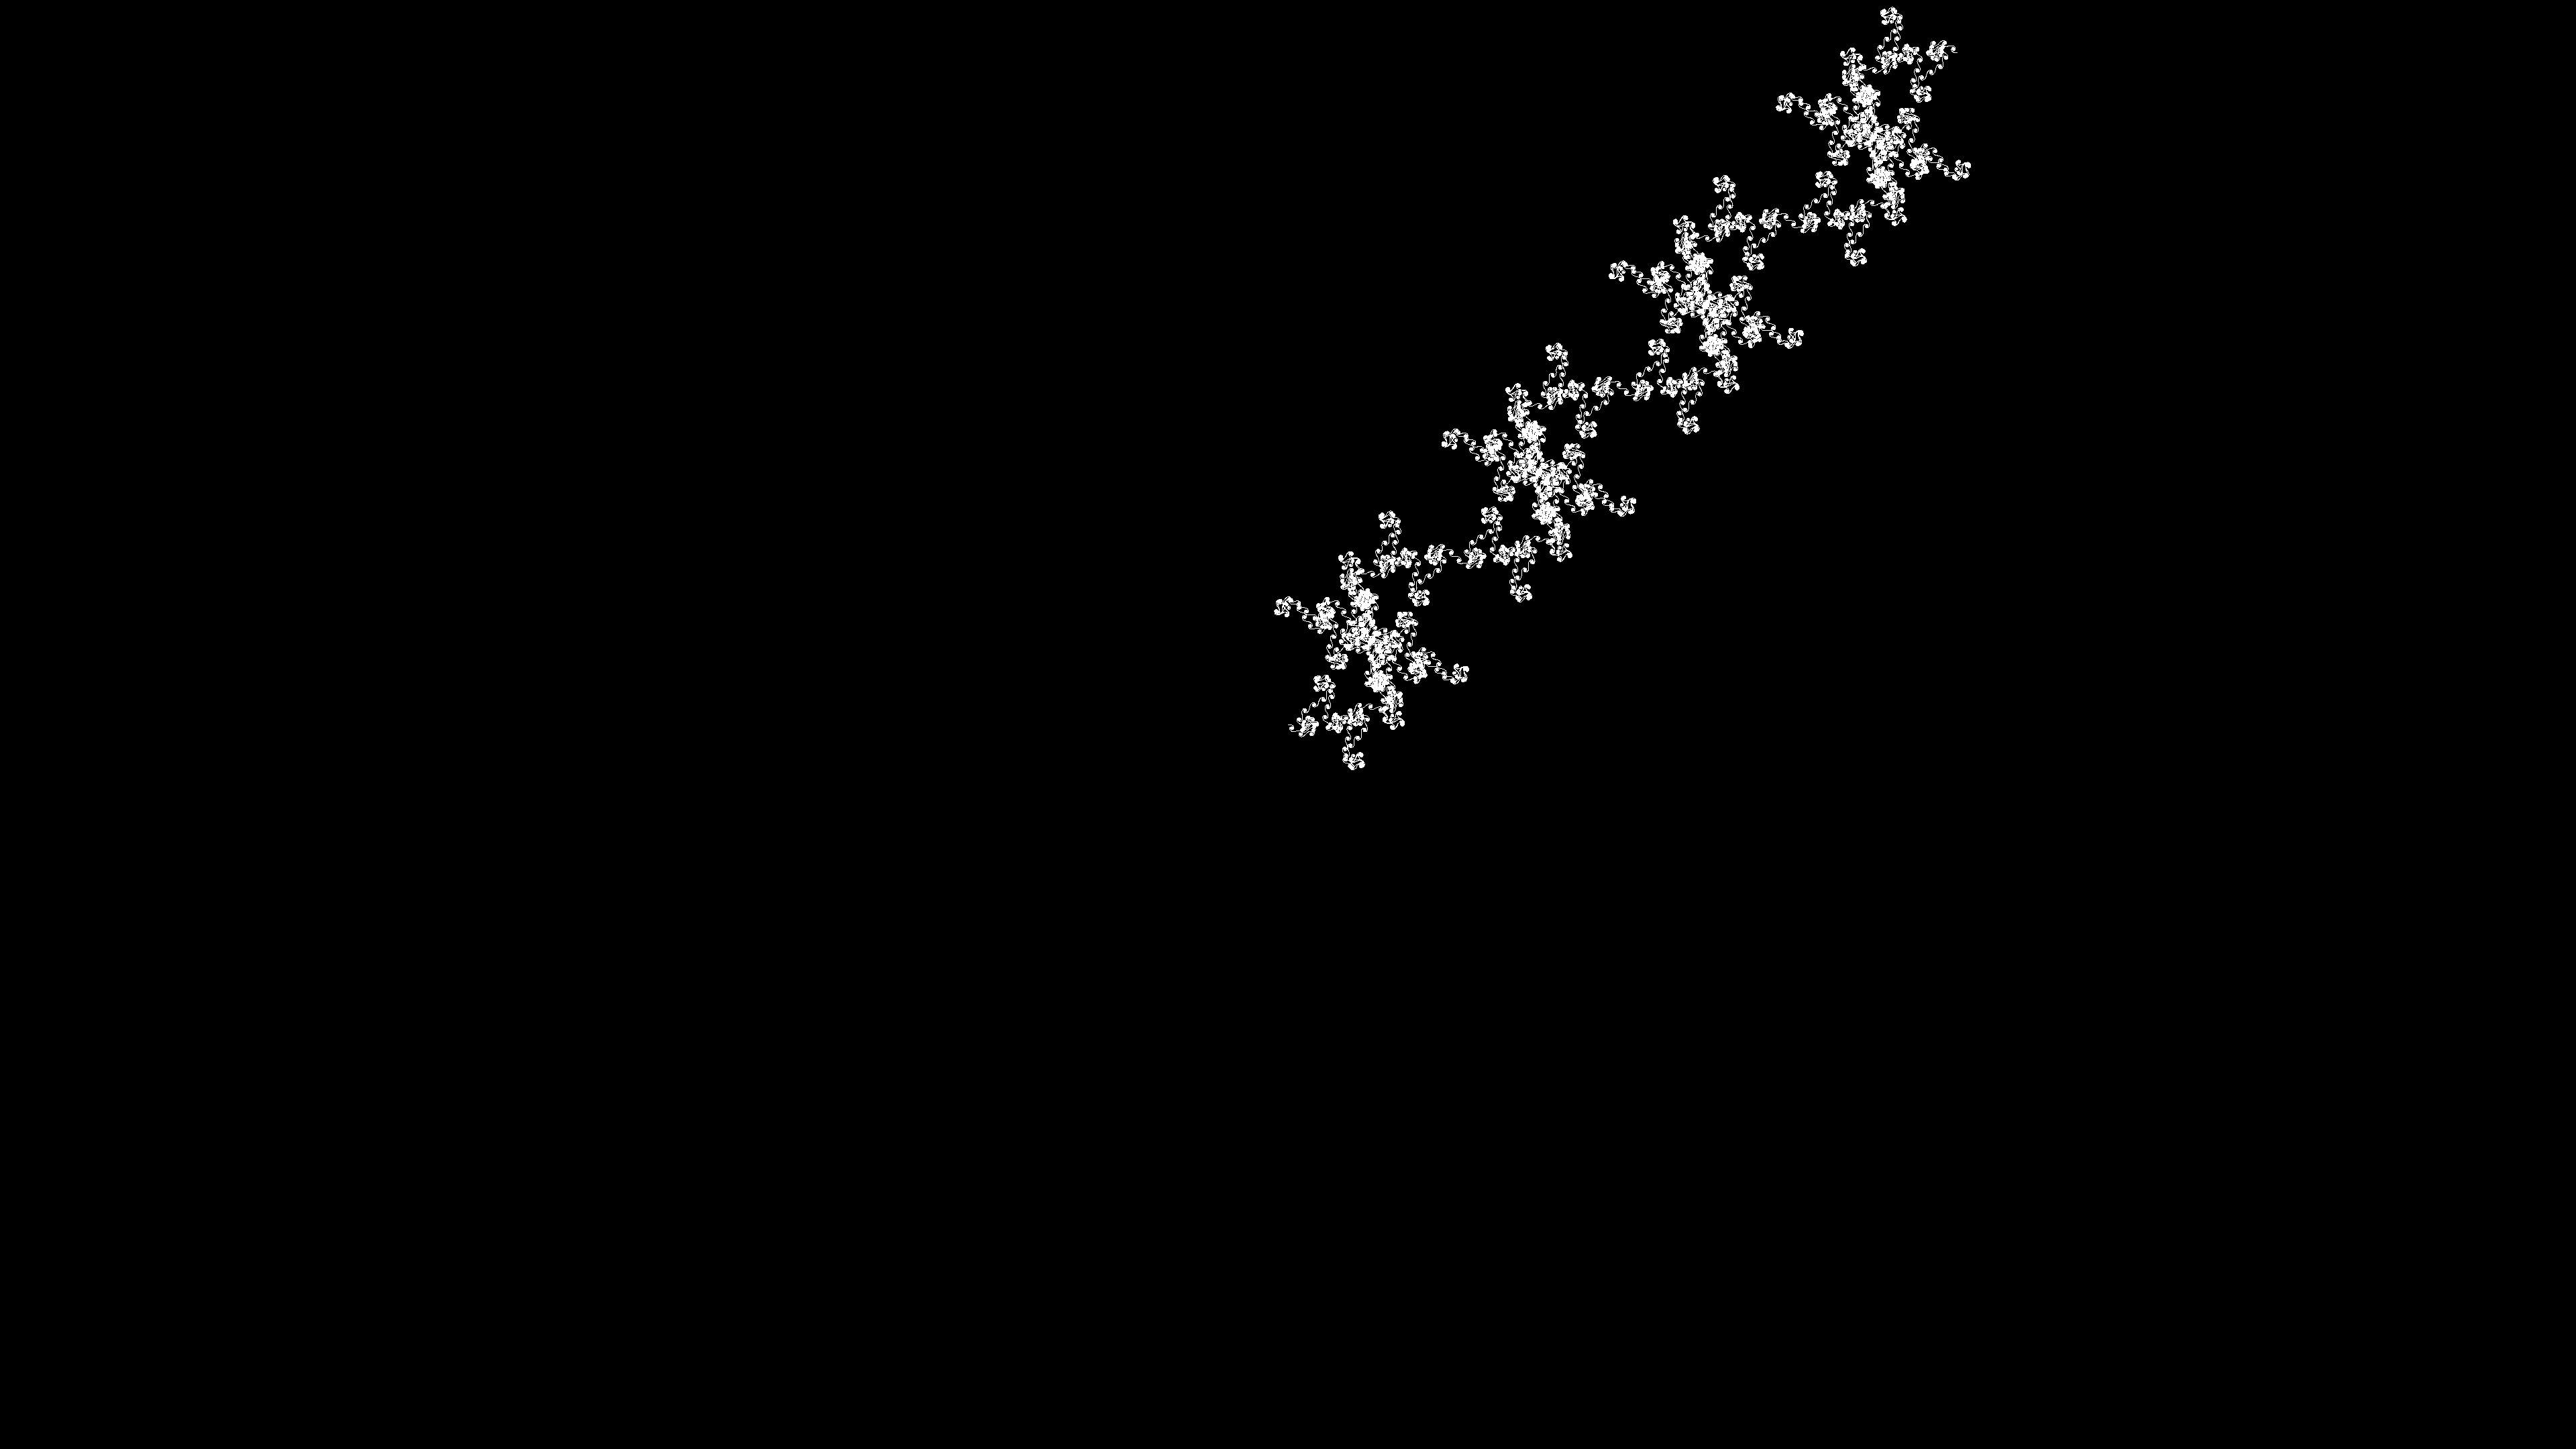
\includegraphics[width=\linewidth]{./stepsplusoneimages/0000000034.png}
    \caption{tf p=499 q=200131 theta=000 89761206.png}
  \end{subfigure}
  \caption{n=032 s=400 s+1=401}
  \label{fig:n=032}
\end{figure}
\begin{figure}[H]
  \centering
  \begin{subfigure}[t]{0.48\textwidth}
    \centering
    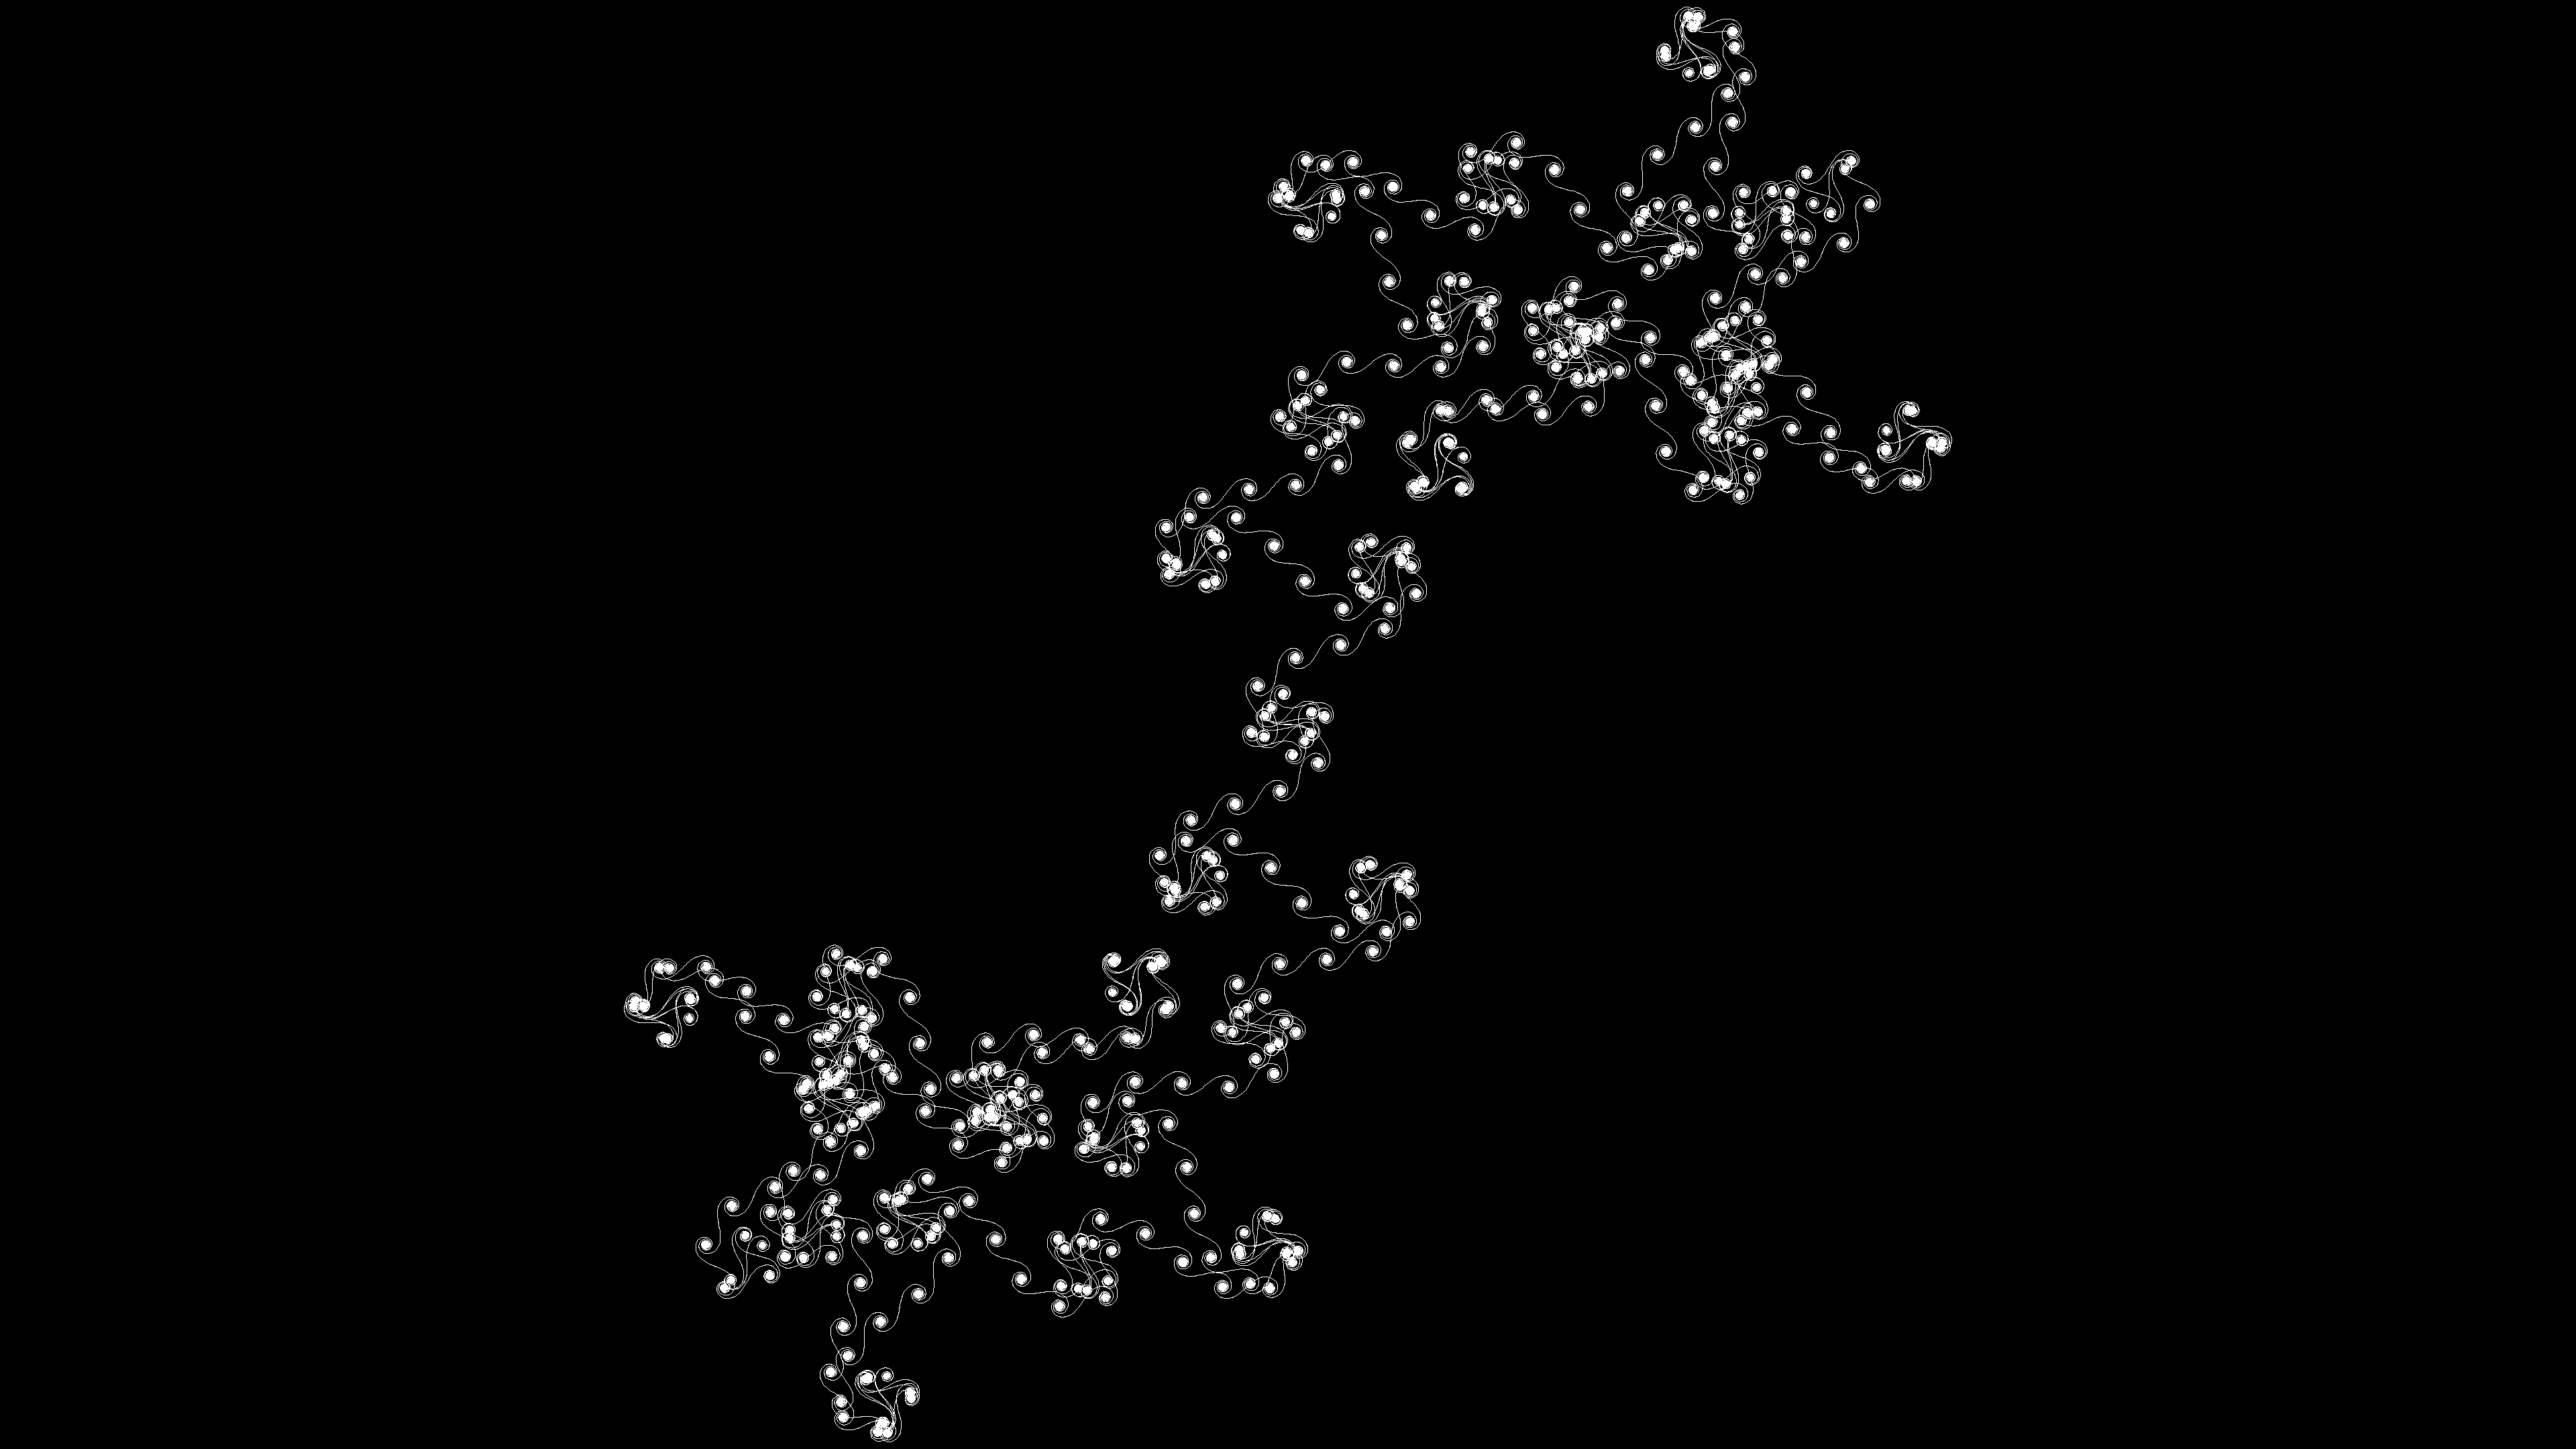
\includegraphics[width=\linewidth]{./stepsplusoneimages/0000000035.png}
    \caption{tf p=499 q=199634 theta=000 89984672.png}
  \end{subfigure}
  \begin{subfigure}[t]{0.48\textwidth}
    \centering
    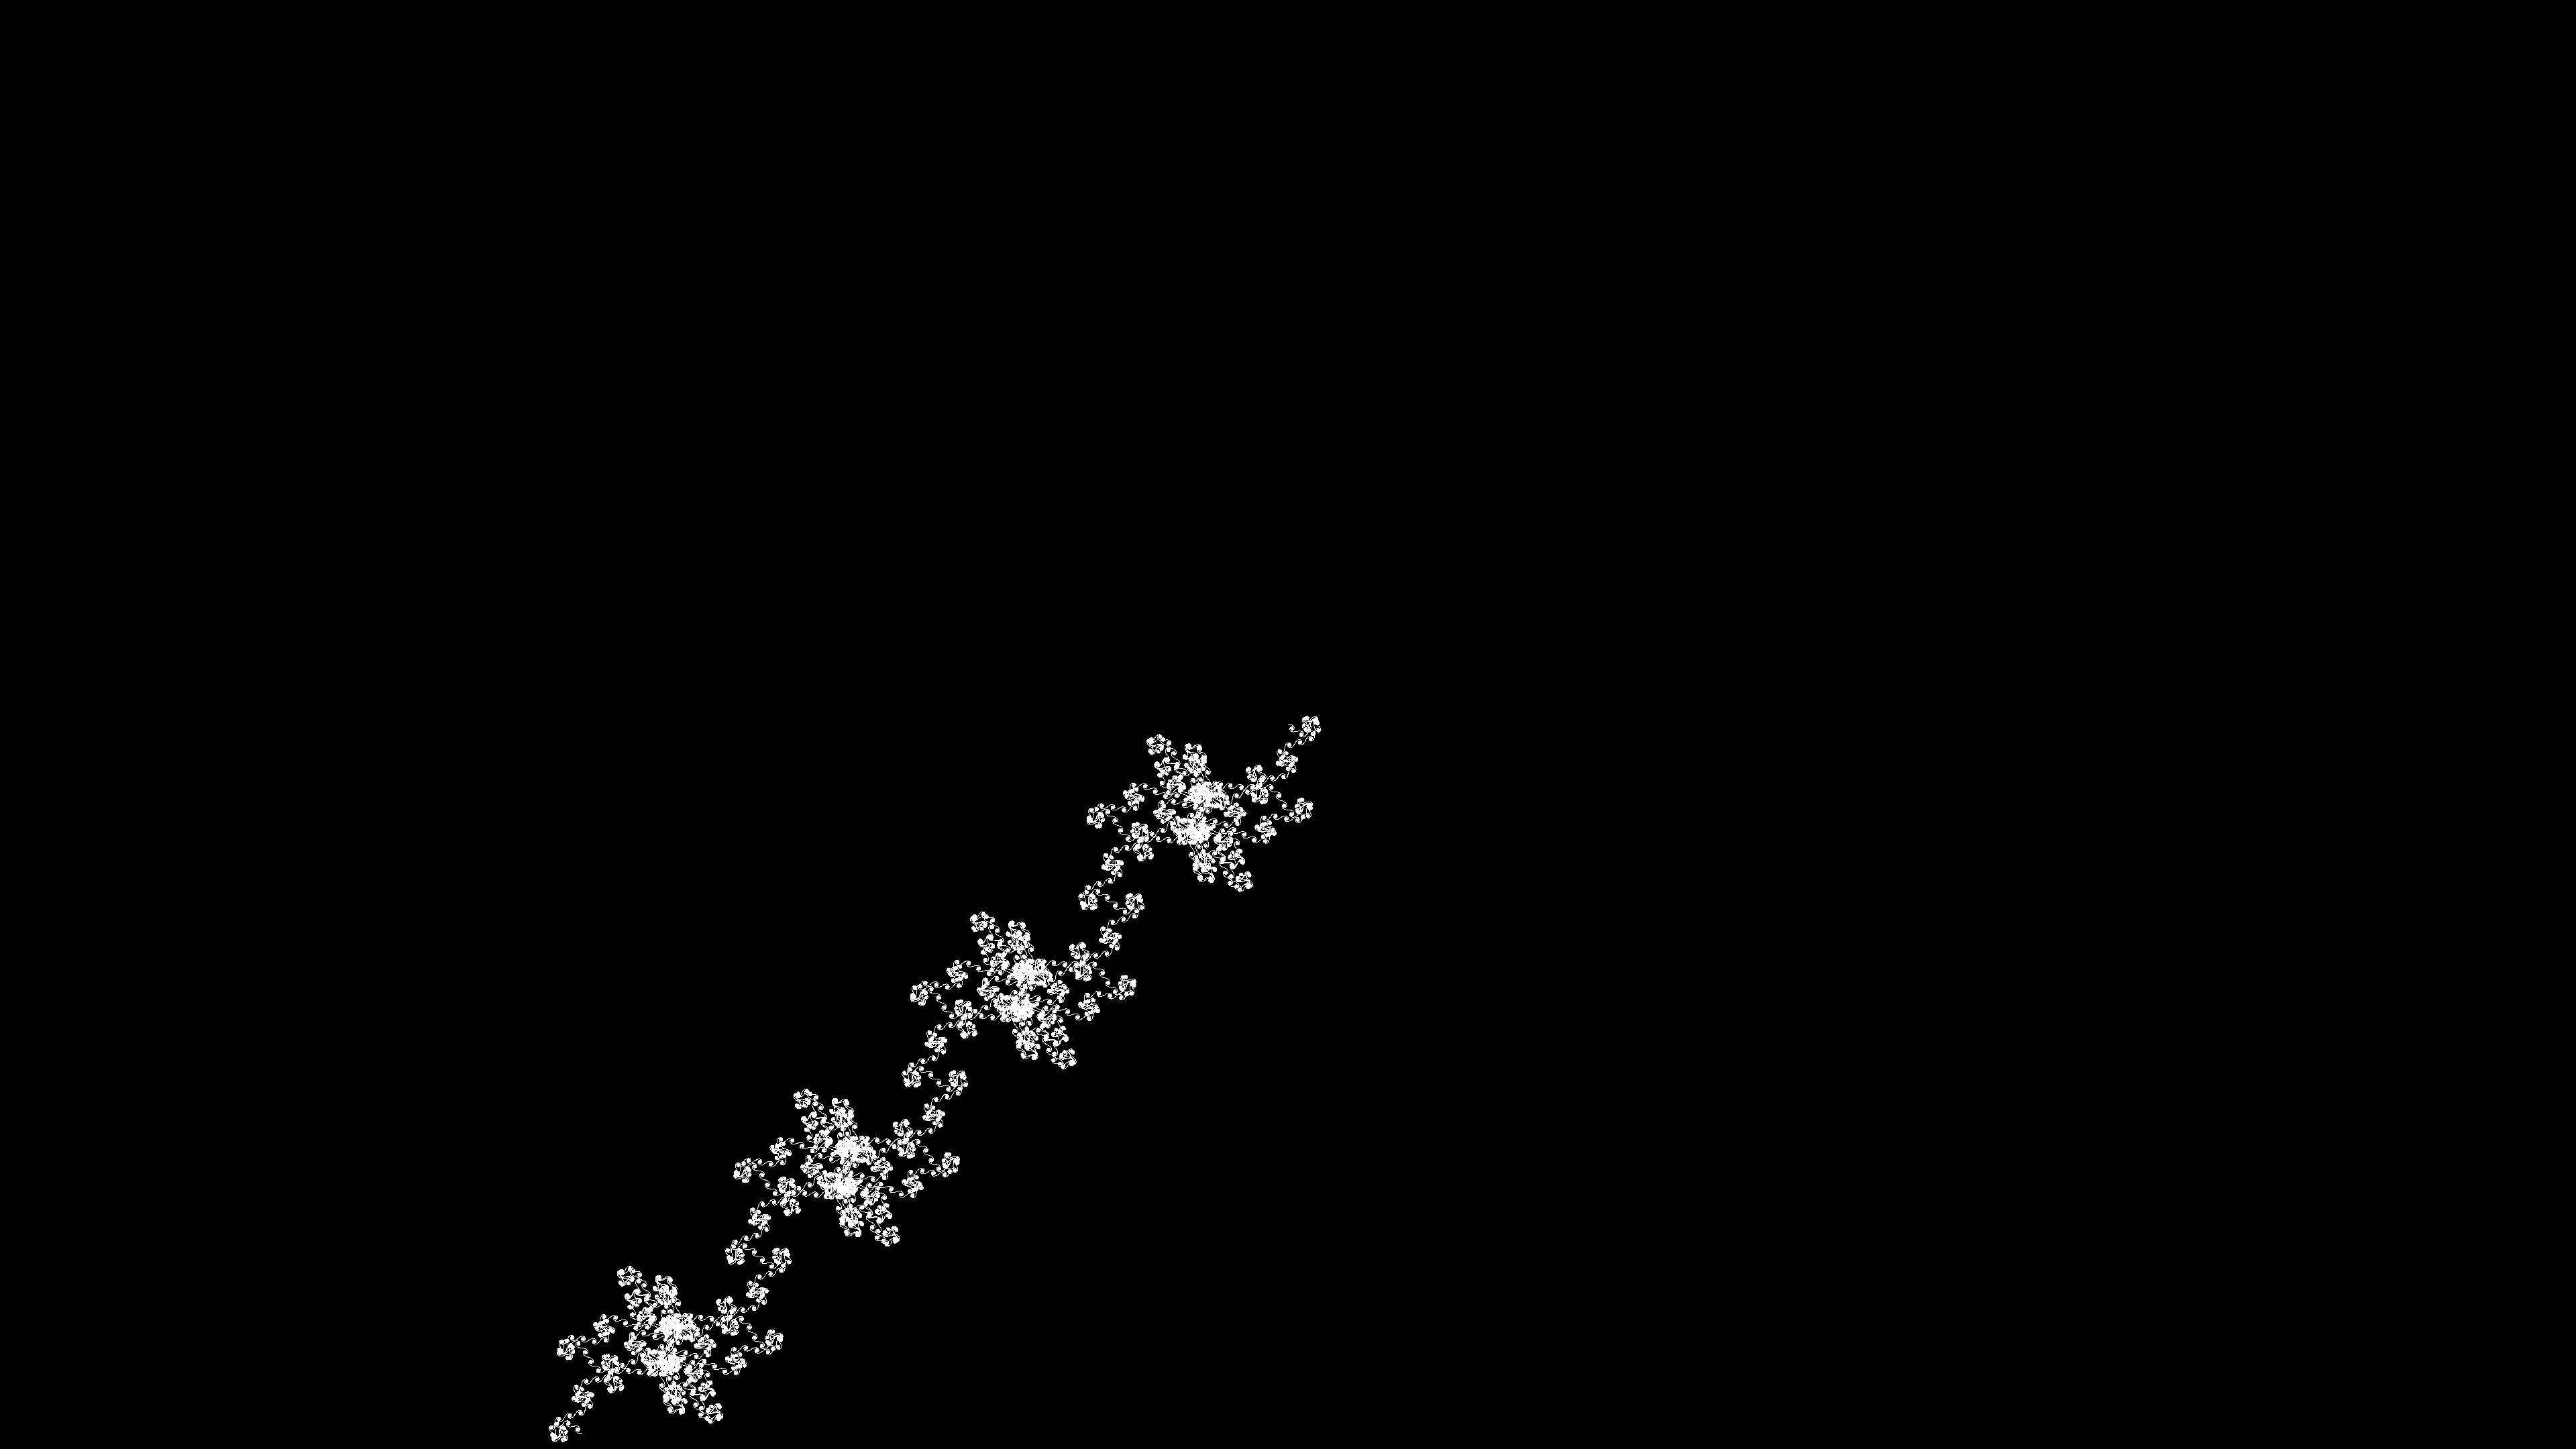
\includegraphics[width=\linewidth]{./stepsplusoneimages/0000000036.png}
    \caption{tf p=499 q=200133 theta=000 89760309.png}
  \end{subfigure}
  \caption{n=034 s=400 s+1=401}
  \label{fig:n=034}
\end{figure}
\begin{figure}[H]
  \centering
  \begin{subfigure}[t]{0.48\textwidth}
    \centering
    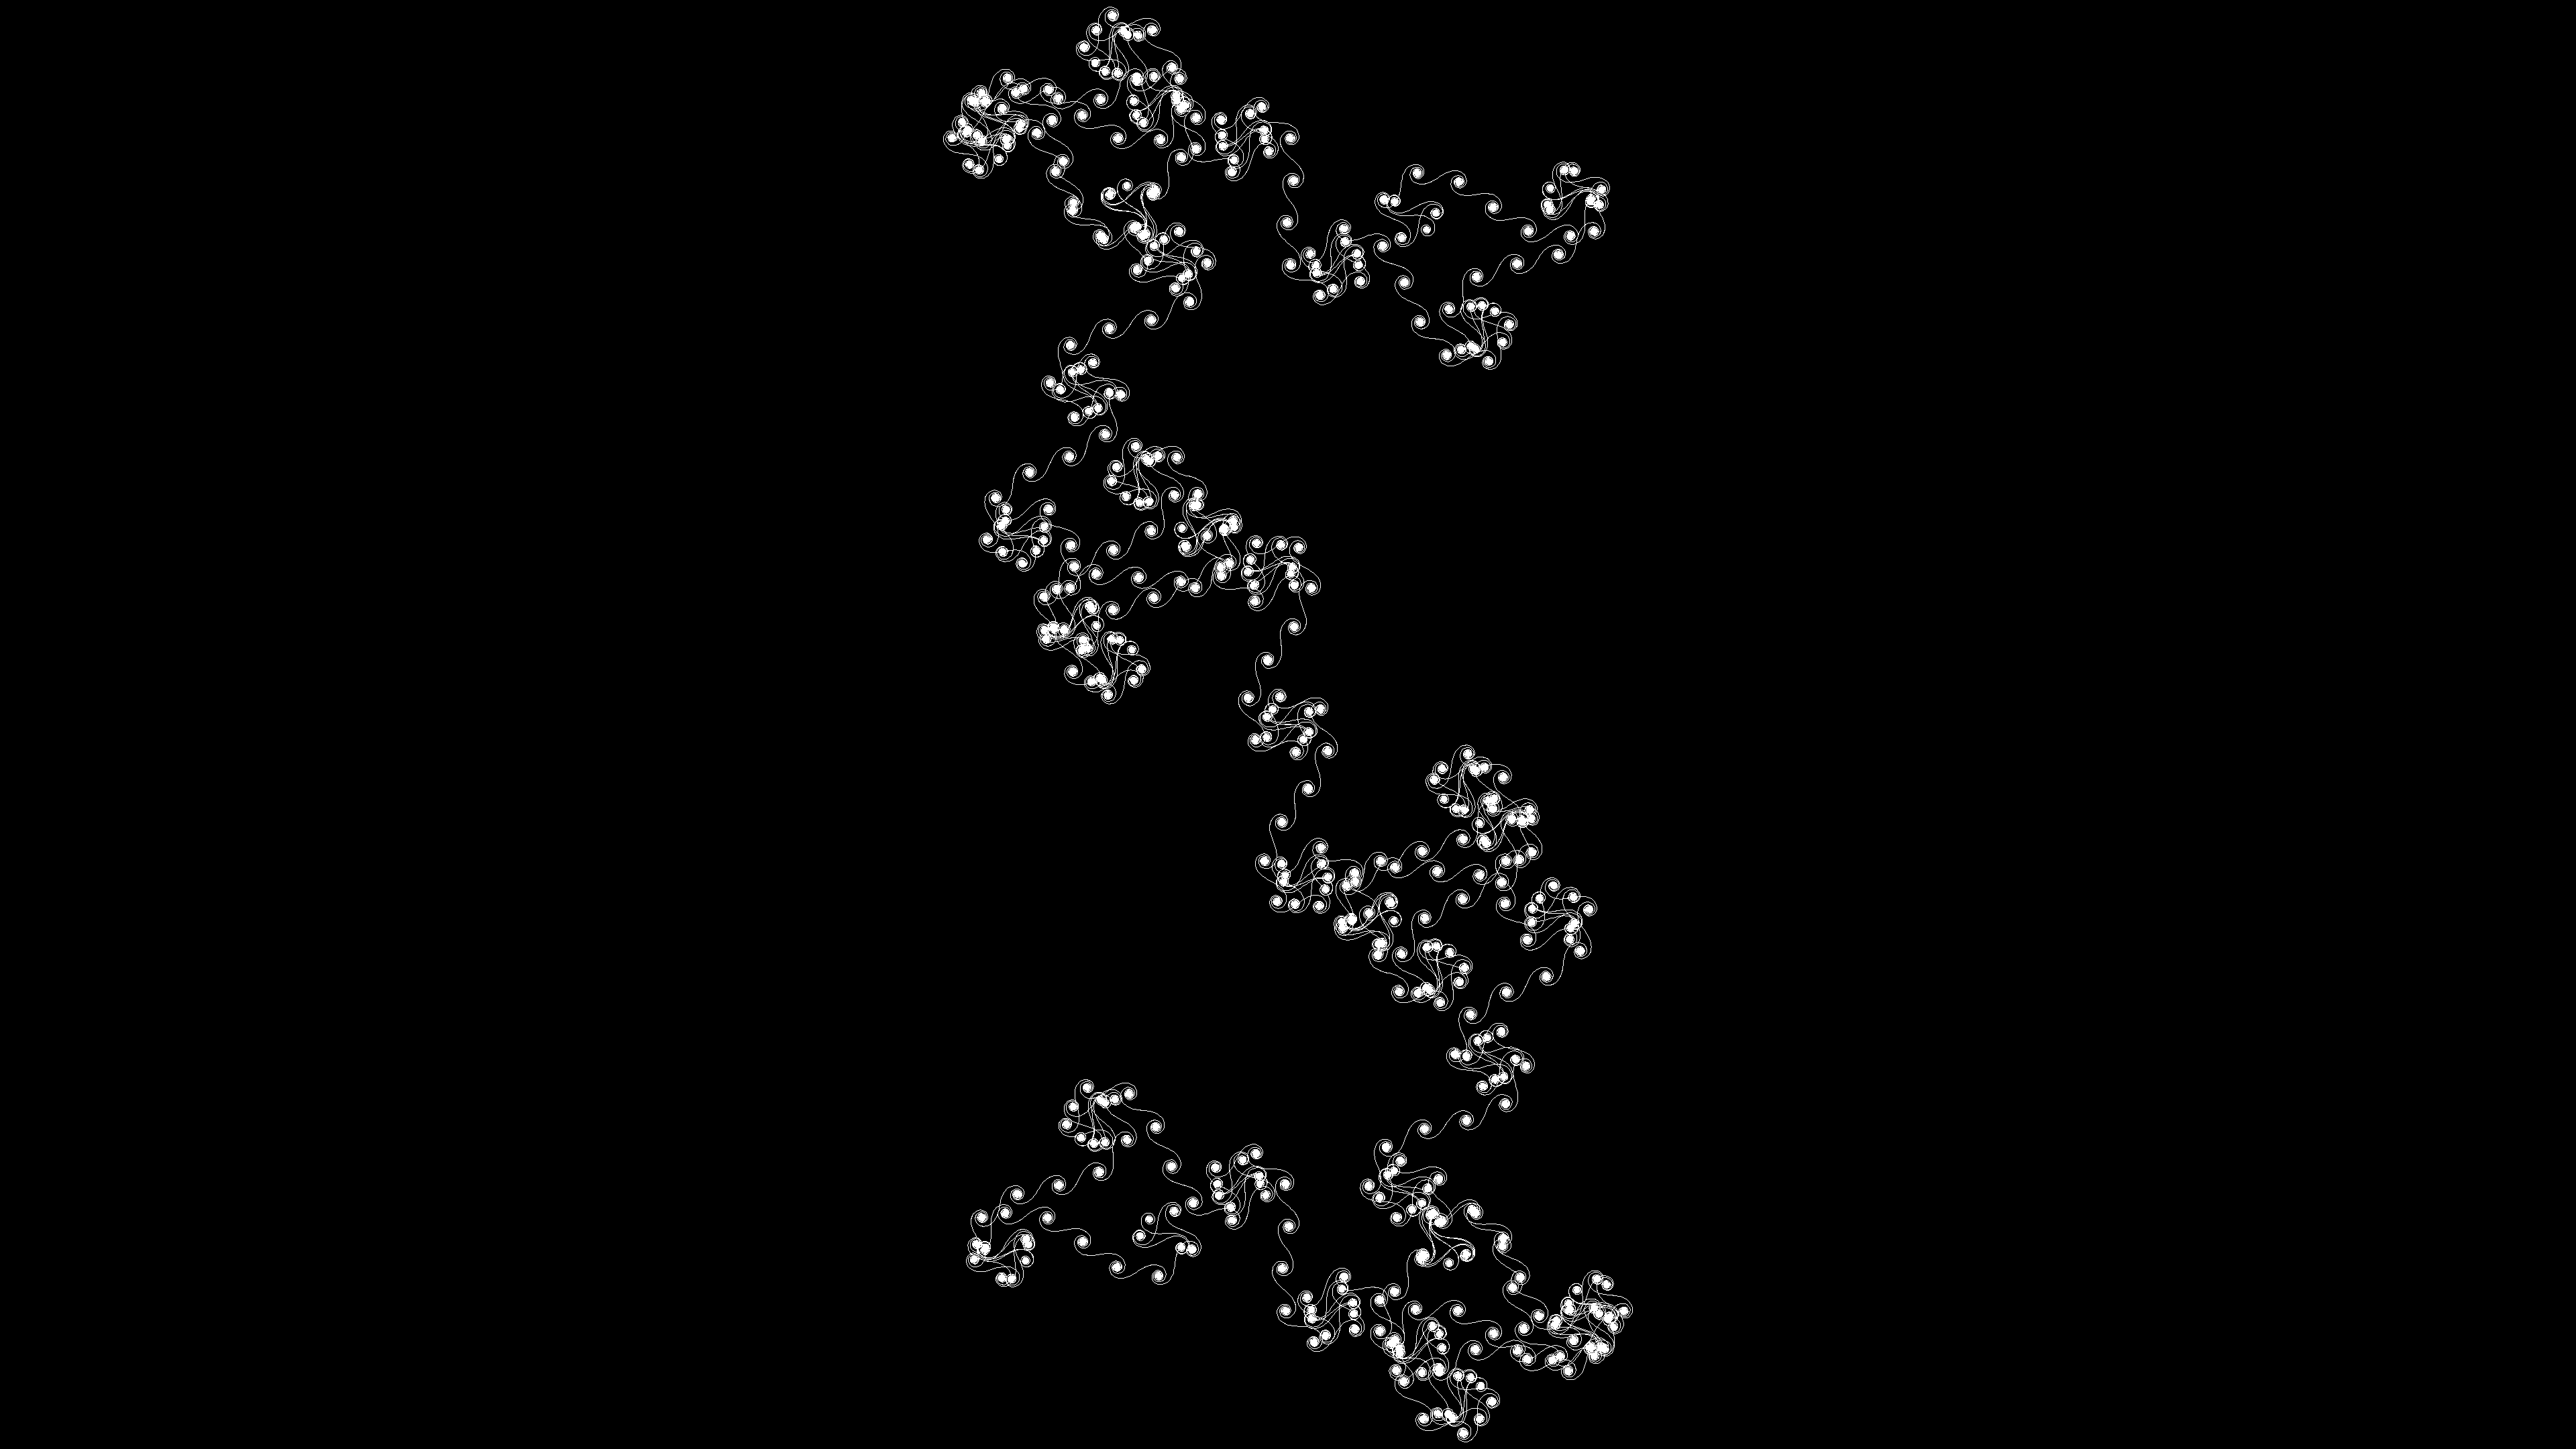
\includegraphics[width=\linewidth]{./stepsplusoneimages/0000000037.png}
    \caption{tf p=499 q=199636 theta=000 89983770.png}
  \end{subfigure}
  \begin{subfigure}[t]{0.48\textwidth}
    \centering
    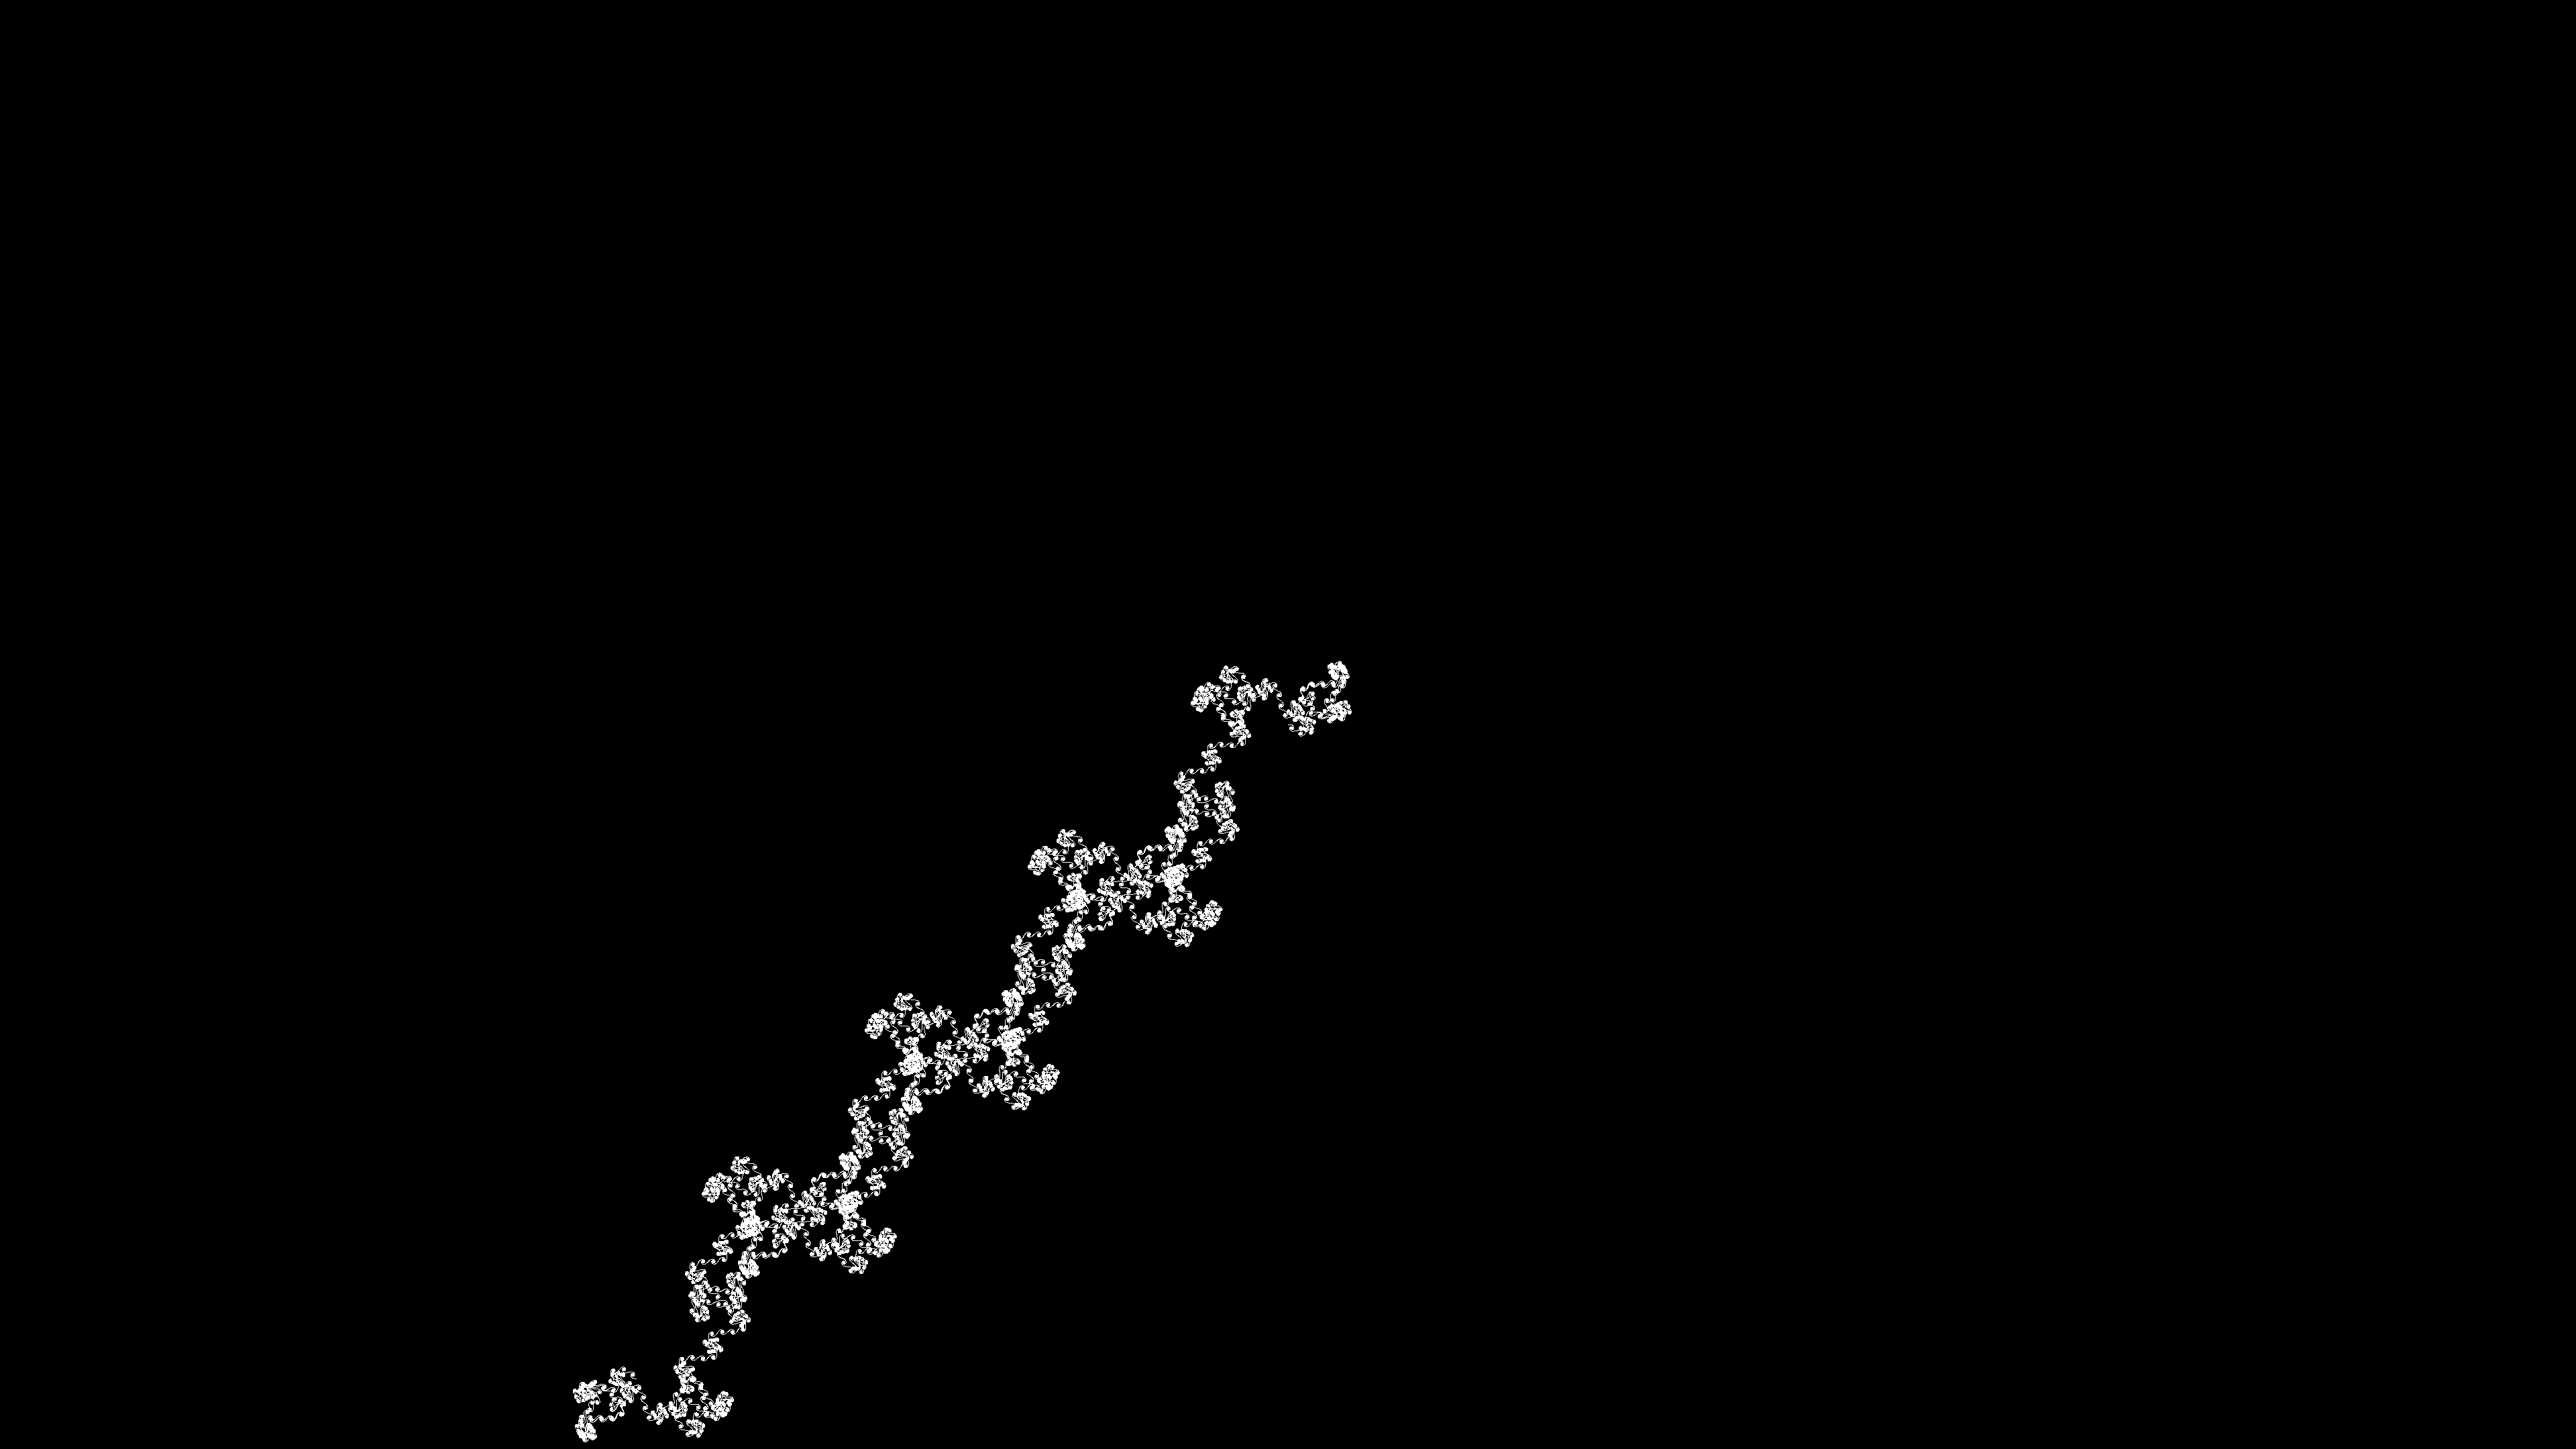
\includegraphics[width=\linewidth]{./stepsplusoneimages/0000000038.png}
    \caption{tf p=499 q=200135 theta=000 89759412.png}
  \end{subfigure}
  \caption{n=036 s=400 s+1=401}
  \label{fig:n=036}
\end{figure}
\begin{figure}[H]
  \centering
  \begin{subfigure}[t]{0.48\textwidth}
    \centering
    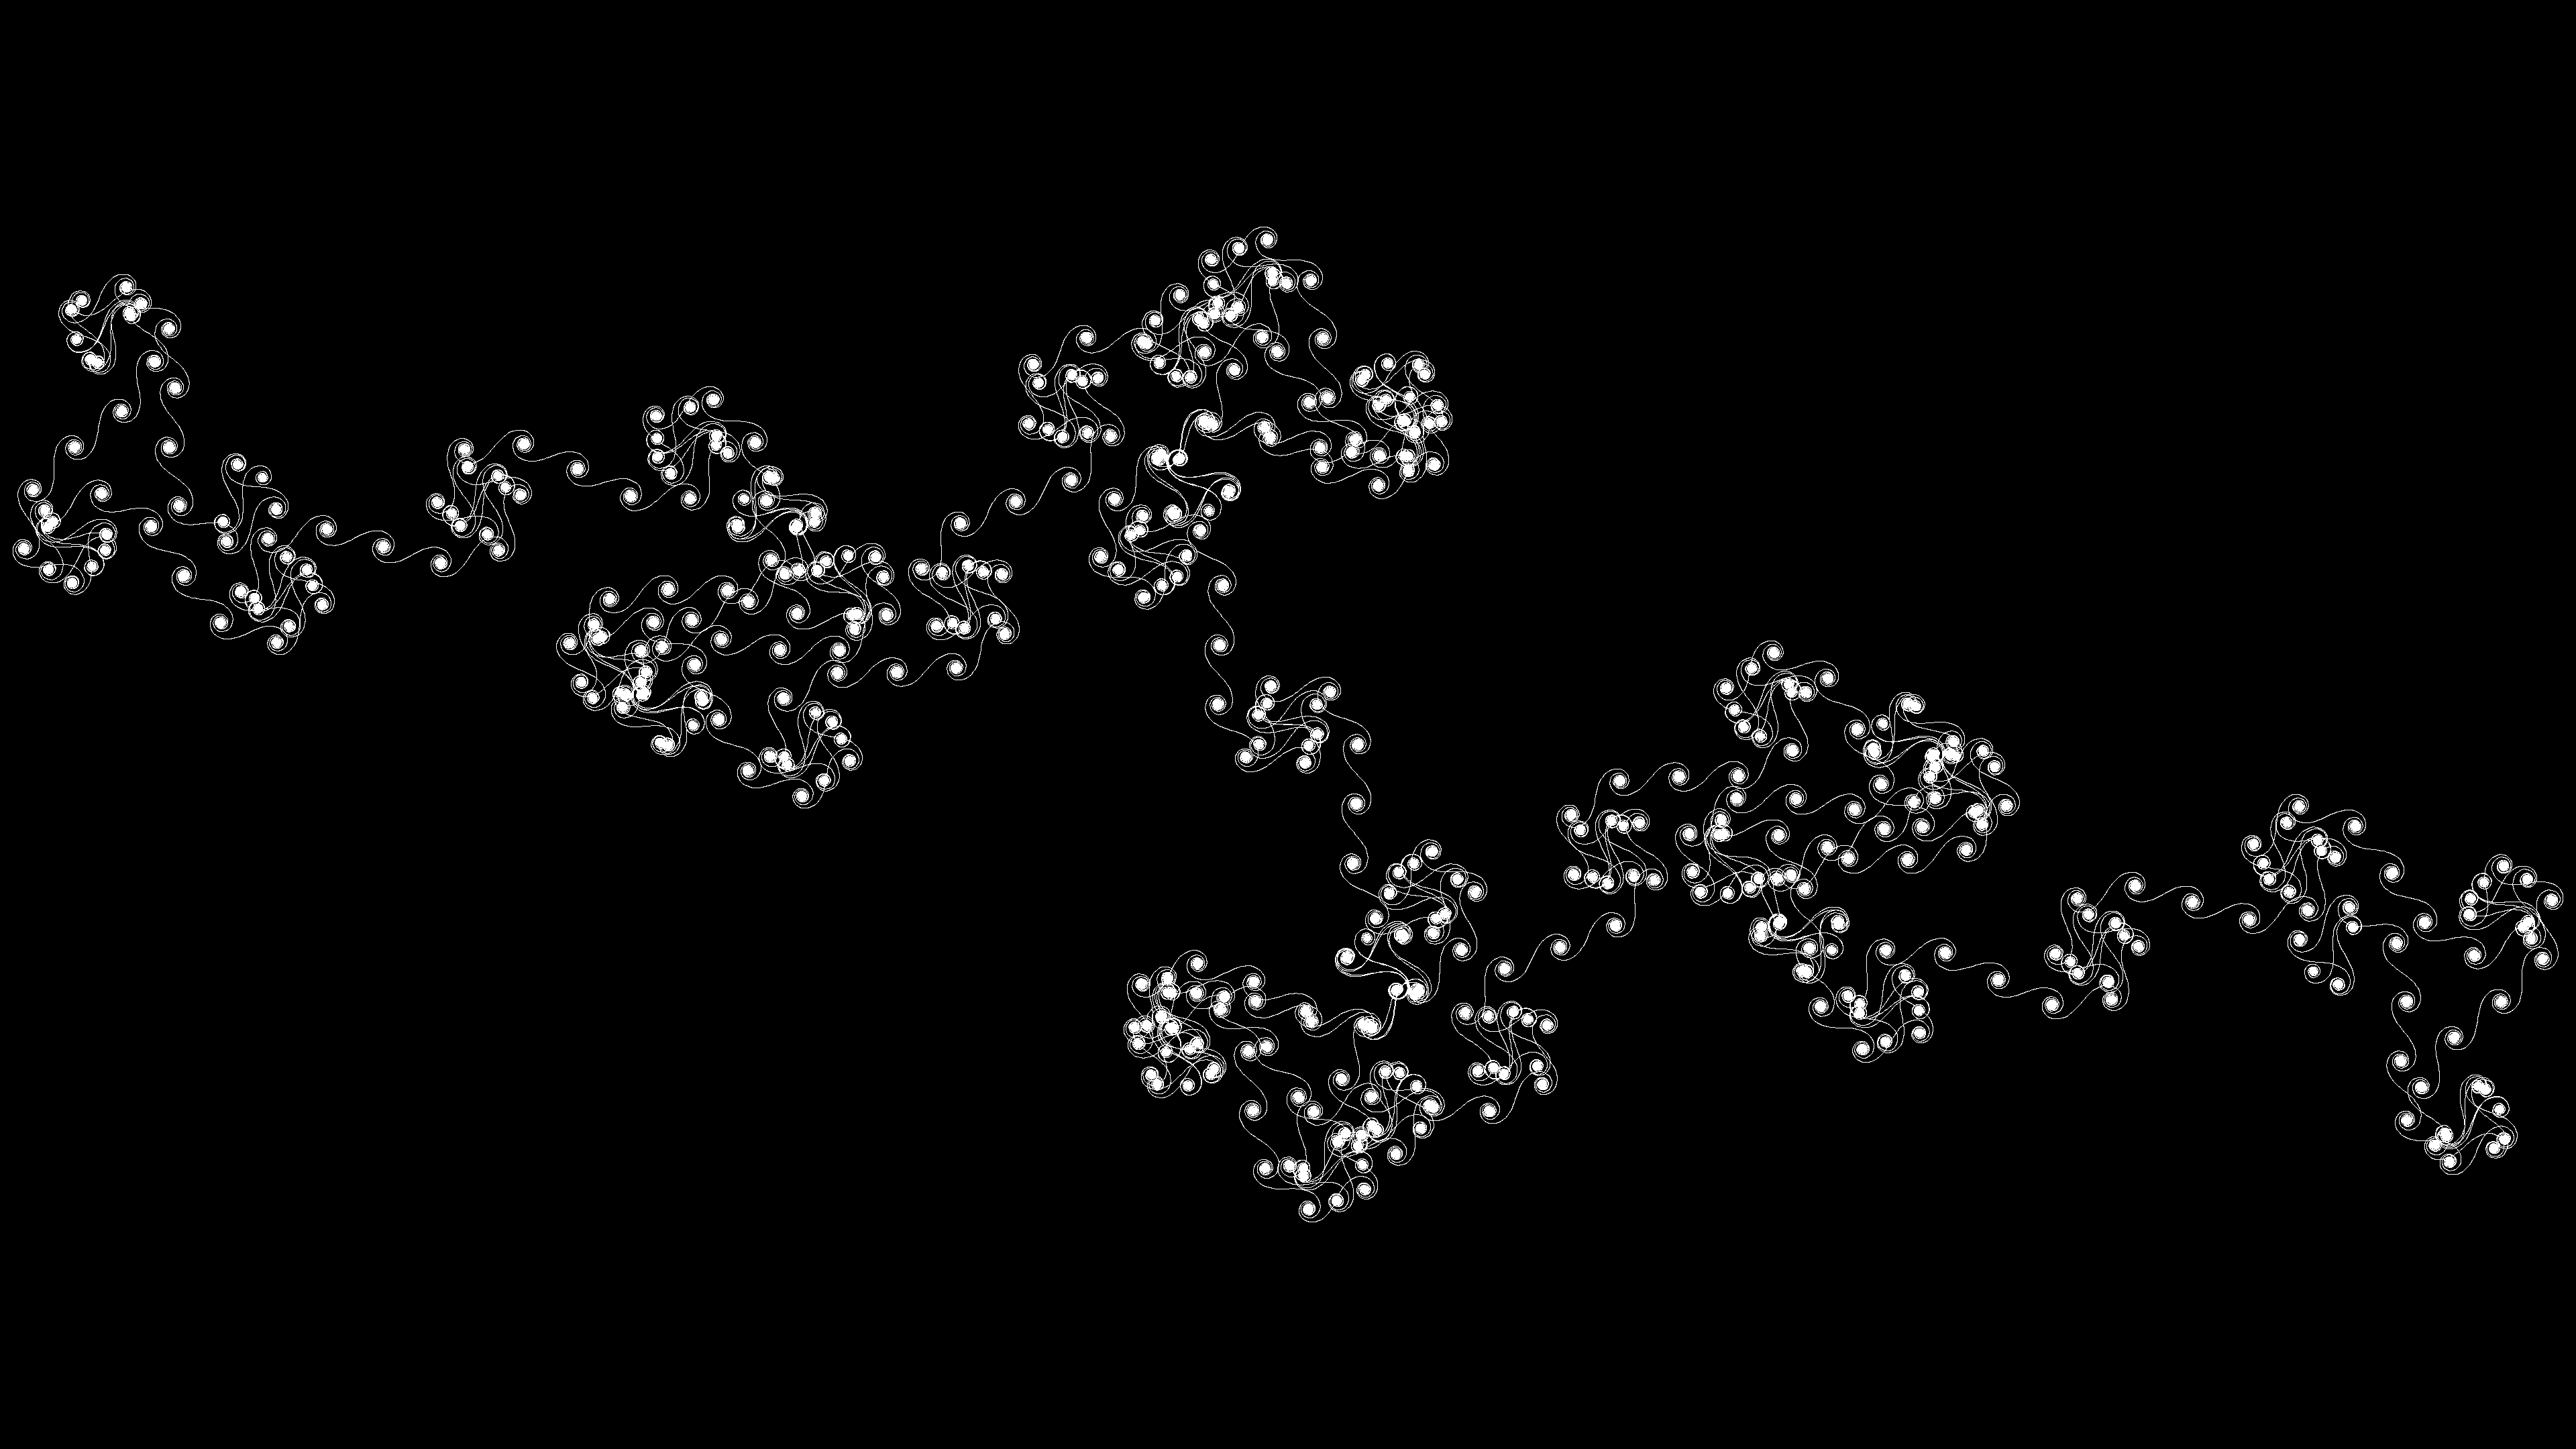
\includegraphics[width=\linewidth]{./stepsplusoneimages/0000000039.png}
    \caption{tf p=499 q=199638 theta=000 89982869.png}
  \end{subfigure}
  \begin{subfigure}[t]{0.48\textwidth}
    \centering
    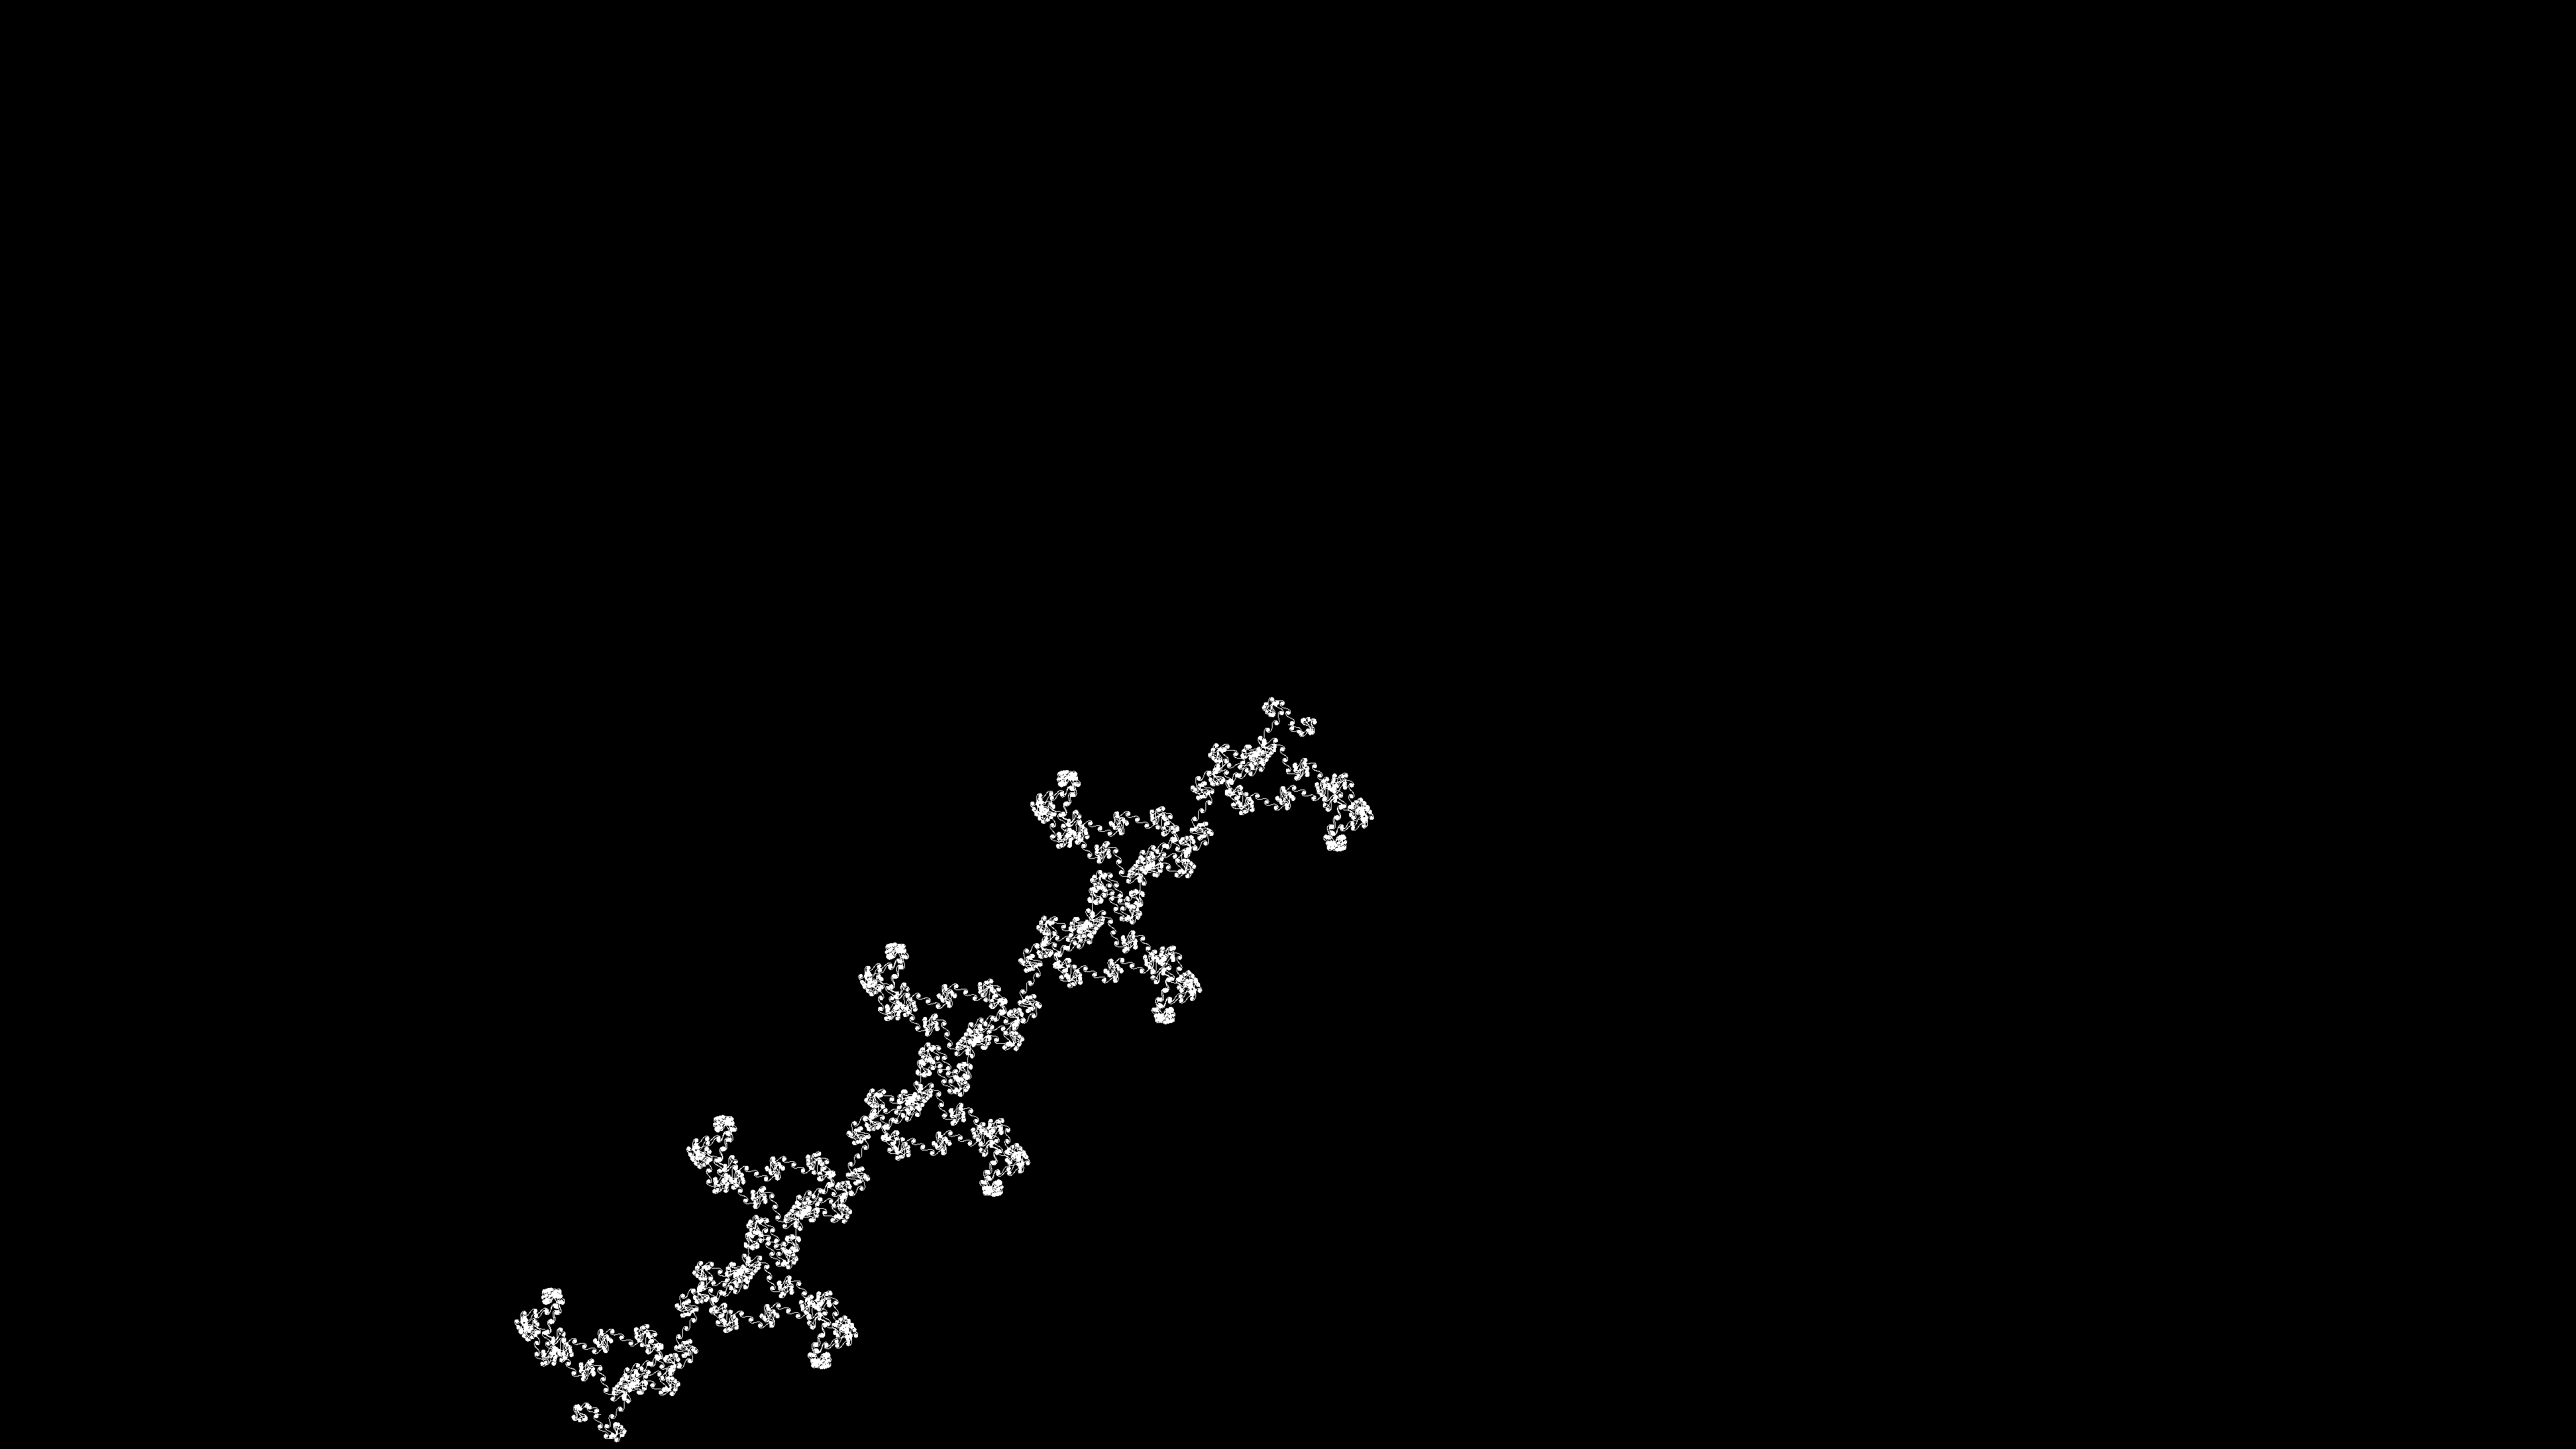
\includegraphics[width=\linewidth]{./stepsplusoneimages/0000000040.png}
    \caption{tf p=499 q=200137 theta=000 89758515.png}
  \end{subfigure}
  \caption{n=038 s=400 s+1=401}
  \label{fig:n=038}
\end{figure}
\begin{figure}[H]
  \centering
  \begin{subfigure}[t]{0.48\textwidth}
    \centering
    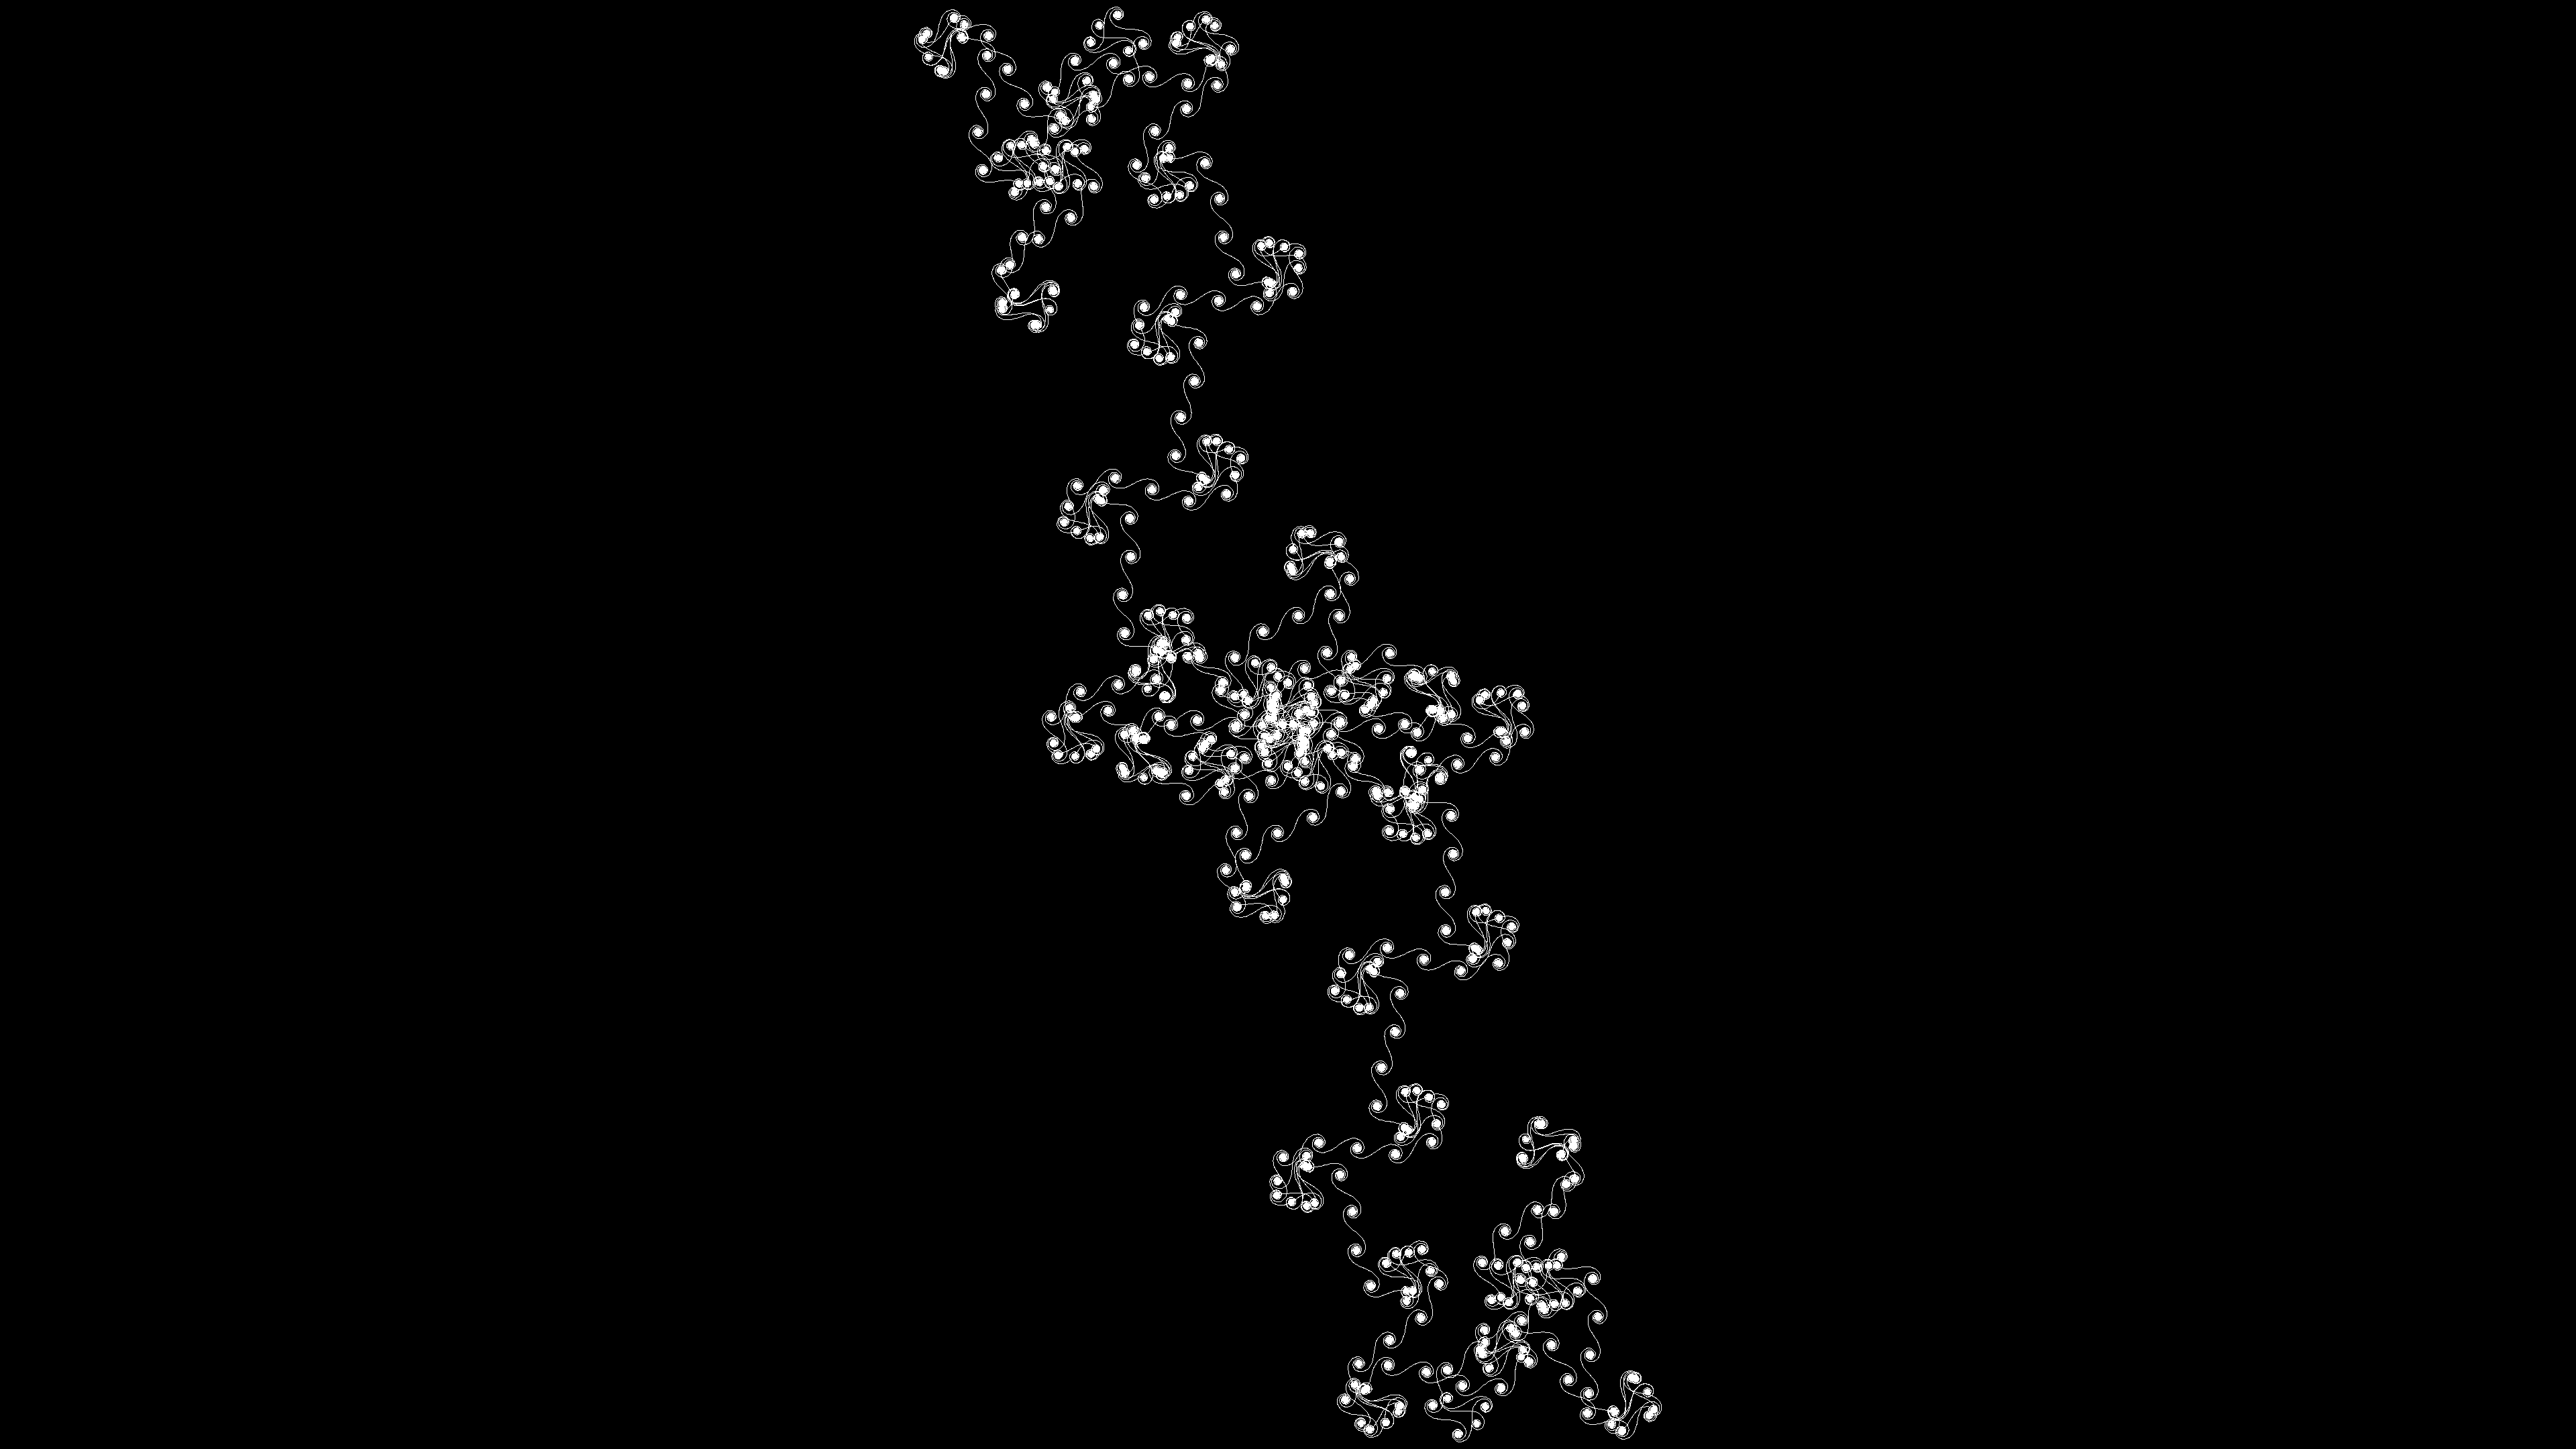
\includegraphics[width=\linewidth]{./stepsplusoneimages/0000000041.png}
    \caption{tf p=499 q=199640 theta=000 89981968.png}
  \end{subfigure}
  \begin{subfigure}[t]{0.48\textwidth}
    \centering
    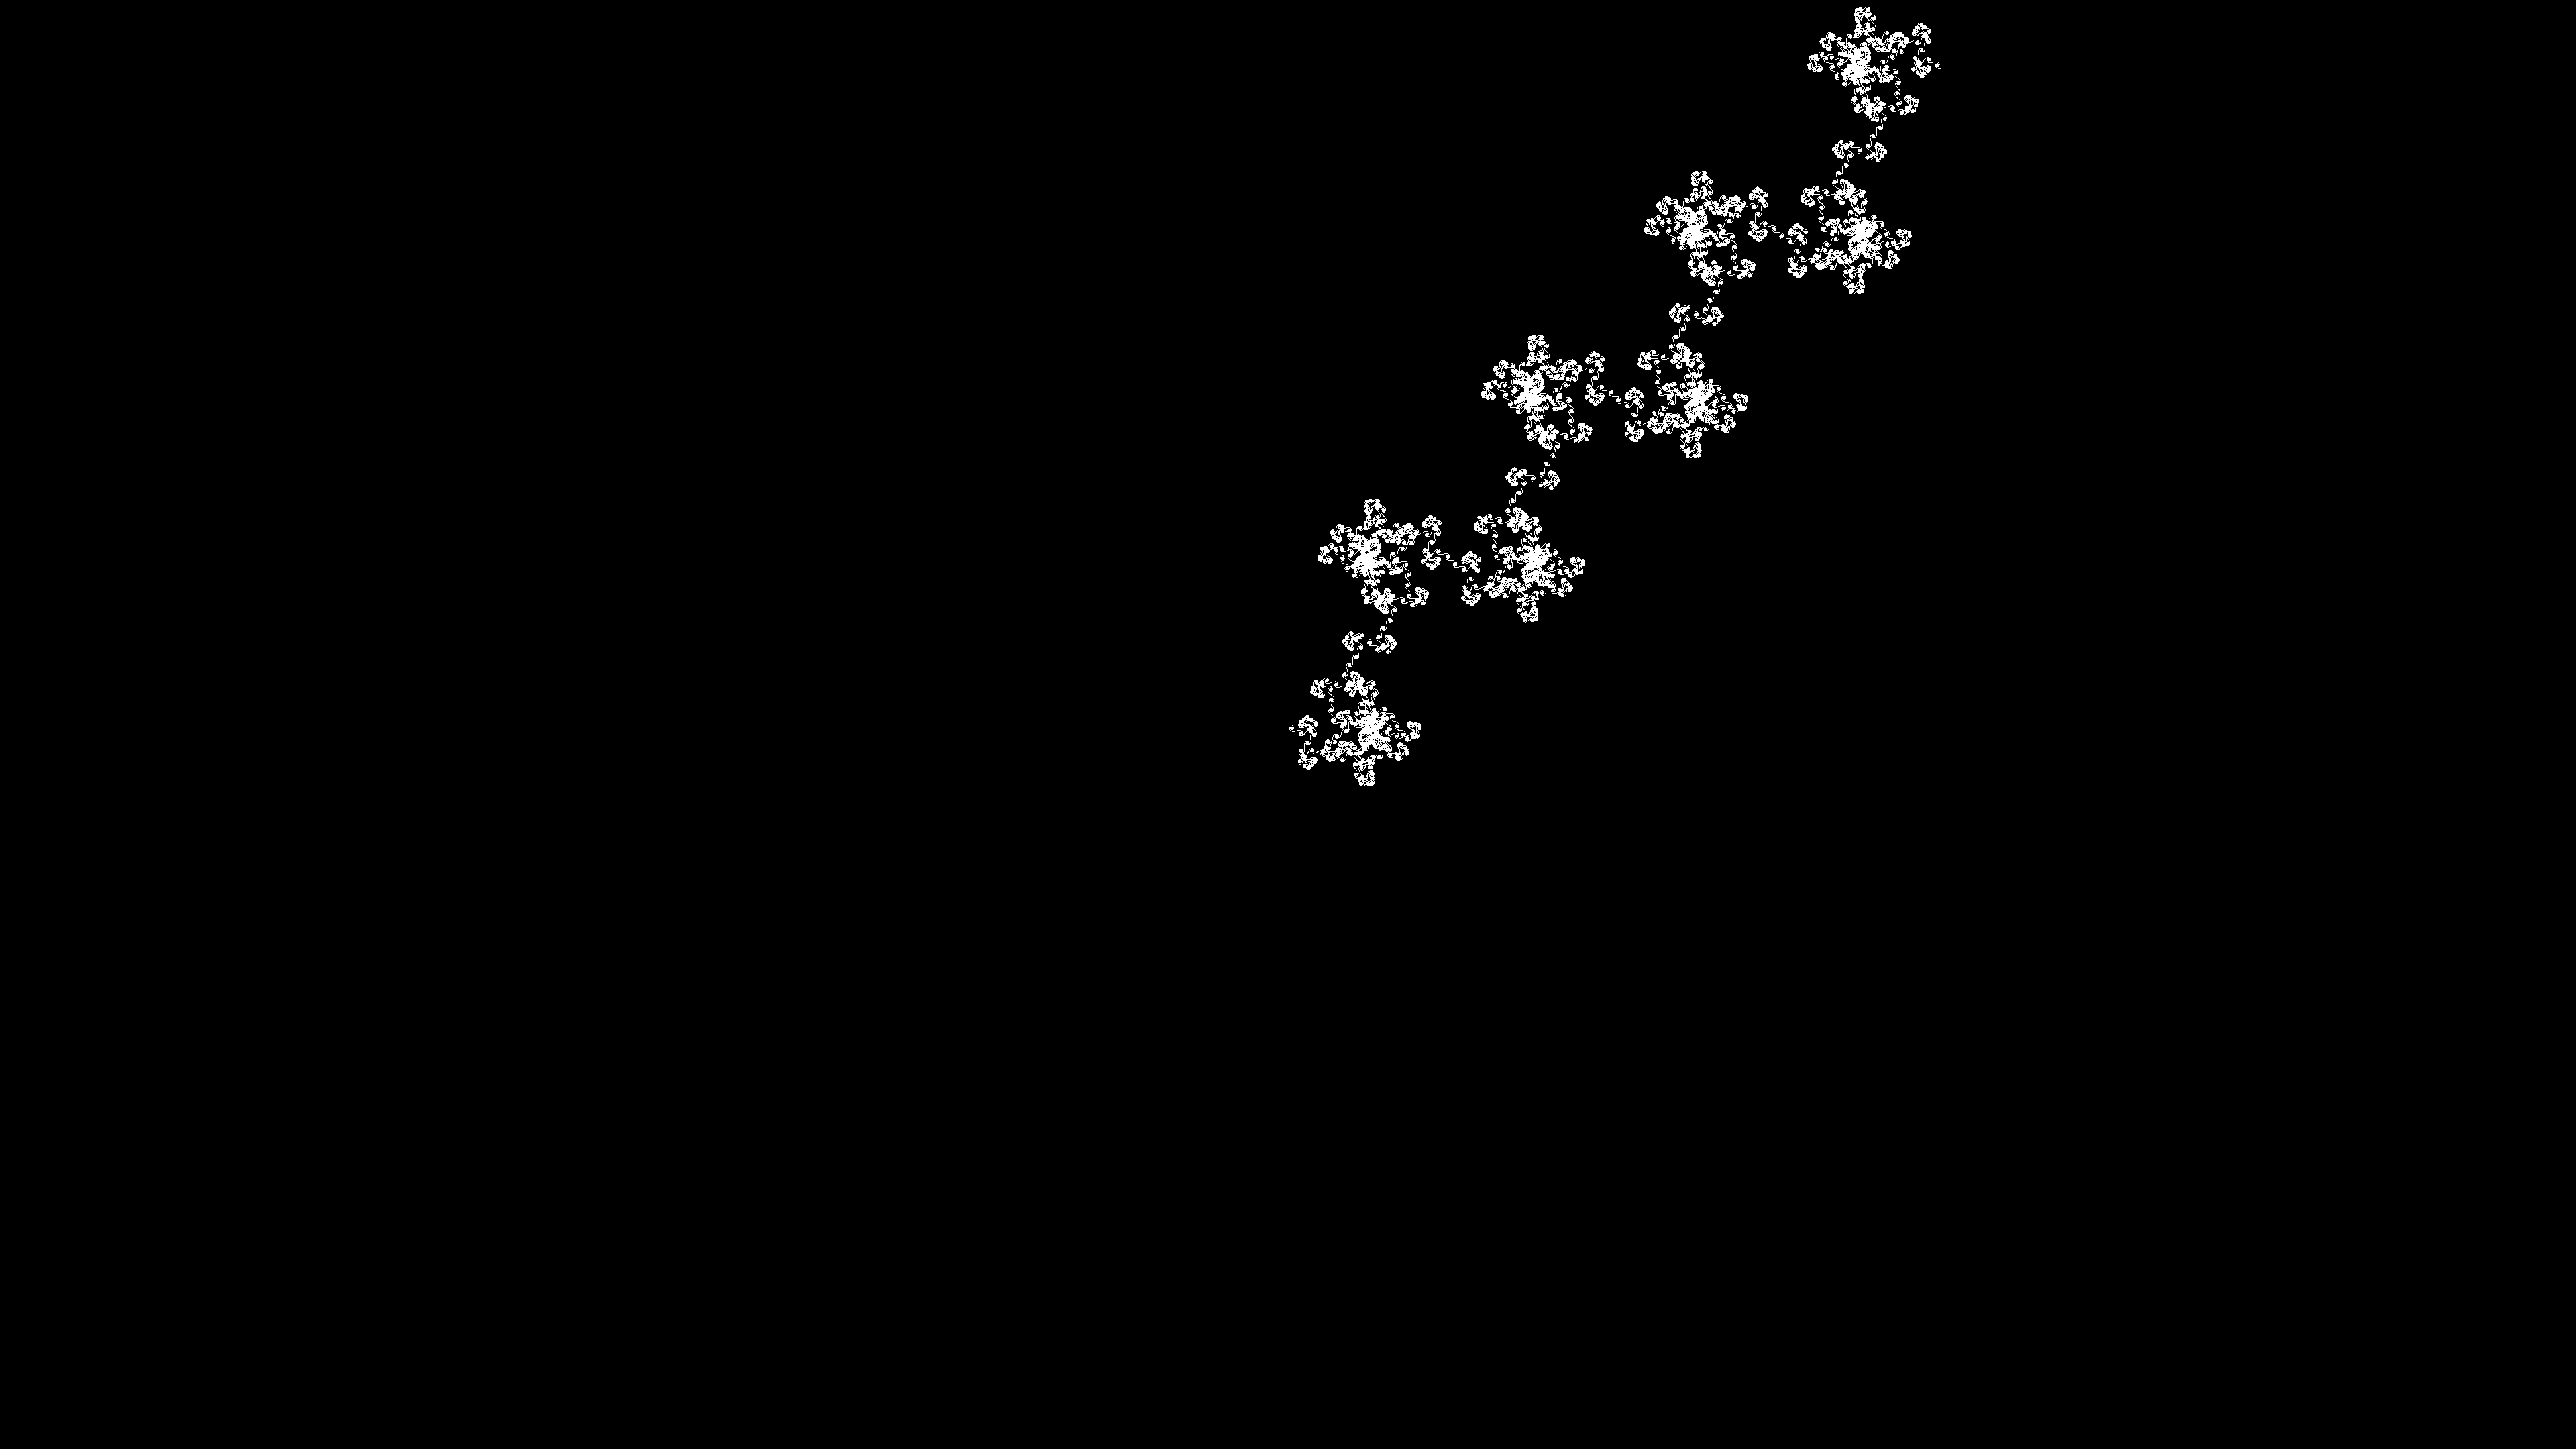
\includegraphics[width=\linewidth]{./stepsplusoneimages/0000000042.png}
    \caption{tf p=499 q=200139 theta=000 89757618.png}
  \end{subfigure}
  \caption{n=040 s=400 s+1=401}
  \label{fig:n=040}
\end{figure}
\begin{figure}[H]
  \centering
  \begin{subfigure}[t]{0.48\textwidth}
    \centering
    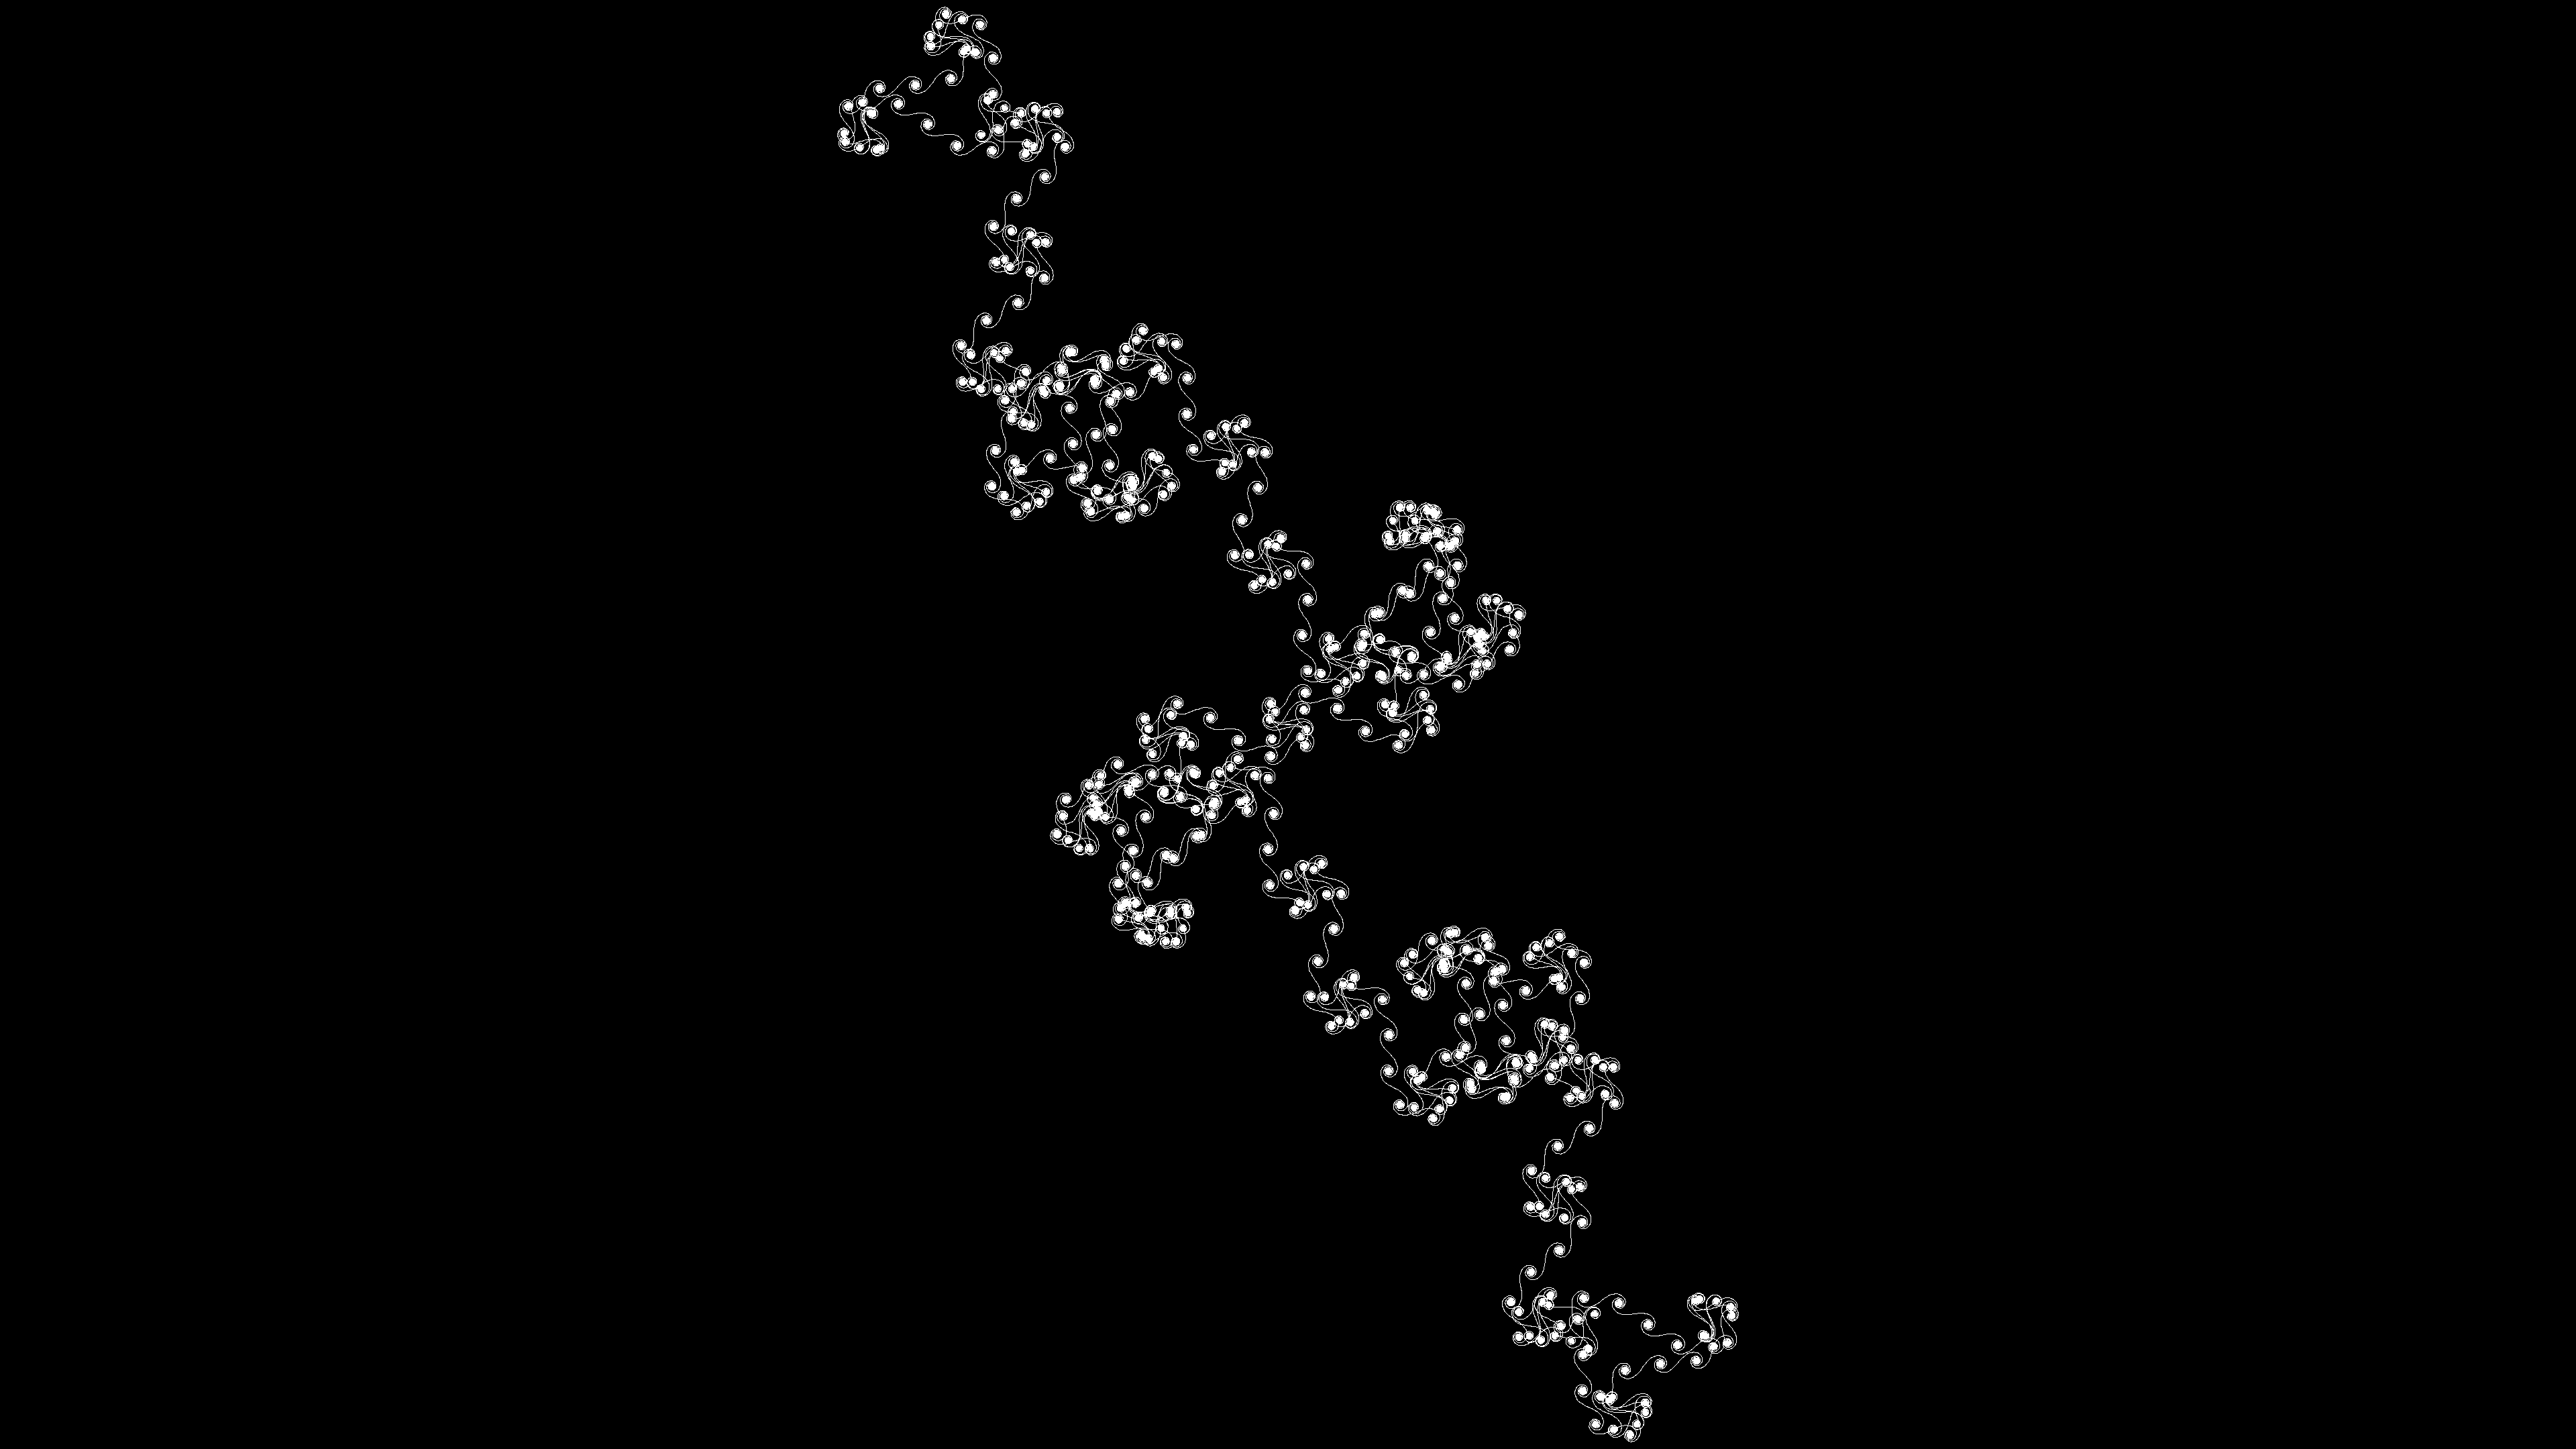
\includegraphics[width=\linewidth]{./stepsplusoneimages/0000000043.png}
    \caption{tf p=499 q=199642 theta=000 89981066.png}
  \end{subfigure}
  \begin{subfigure}[t]{0.48\textwidth}
    \centering
    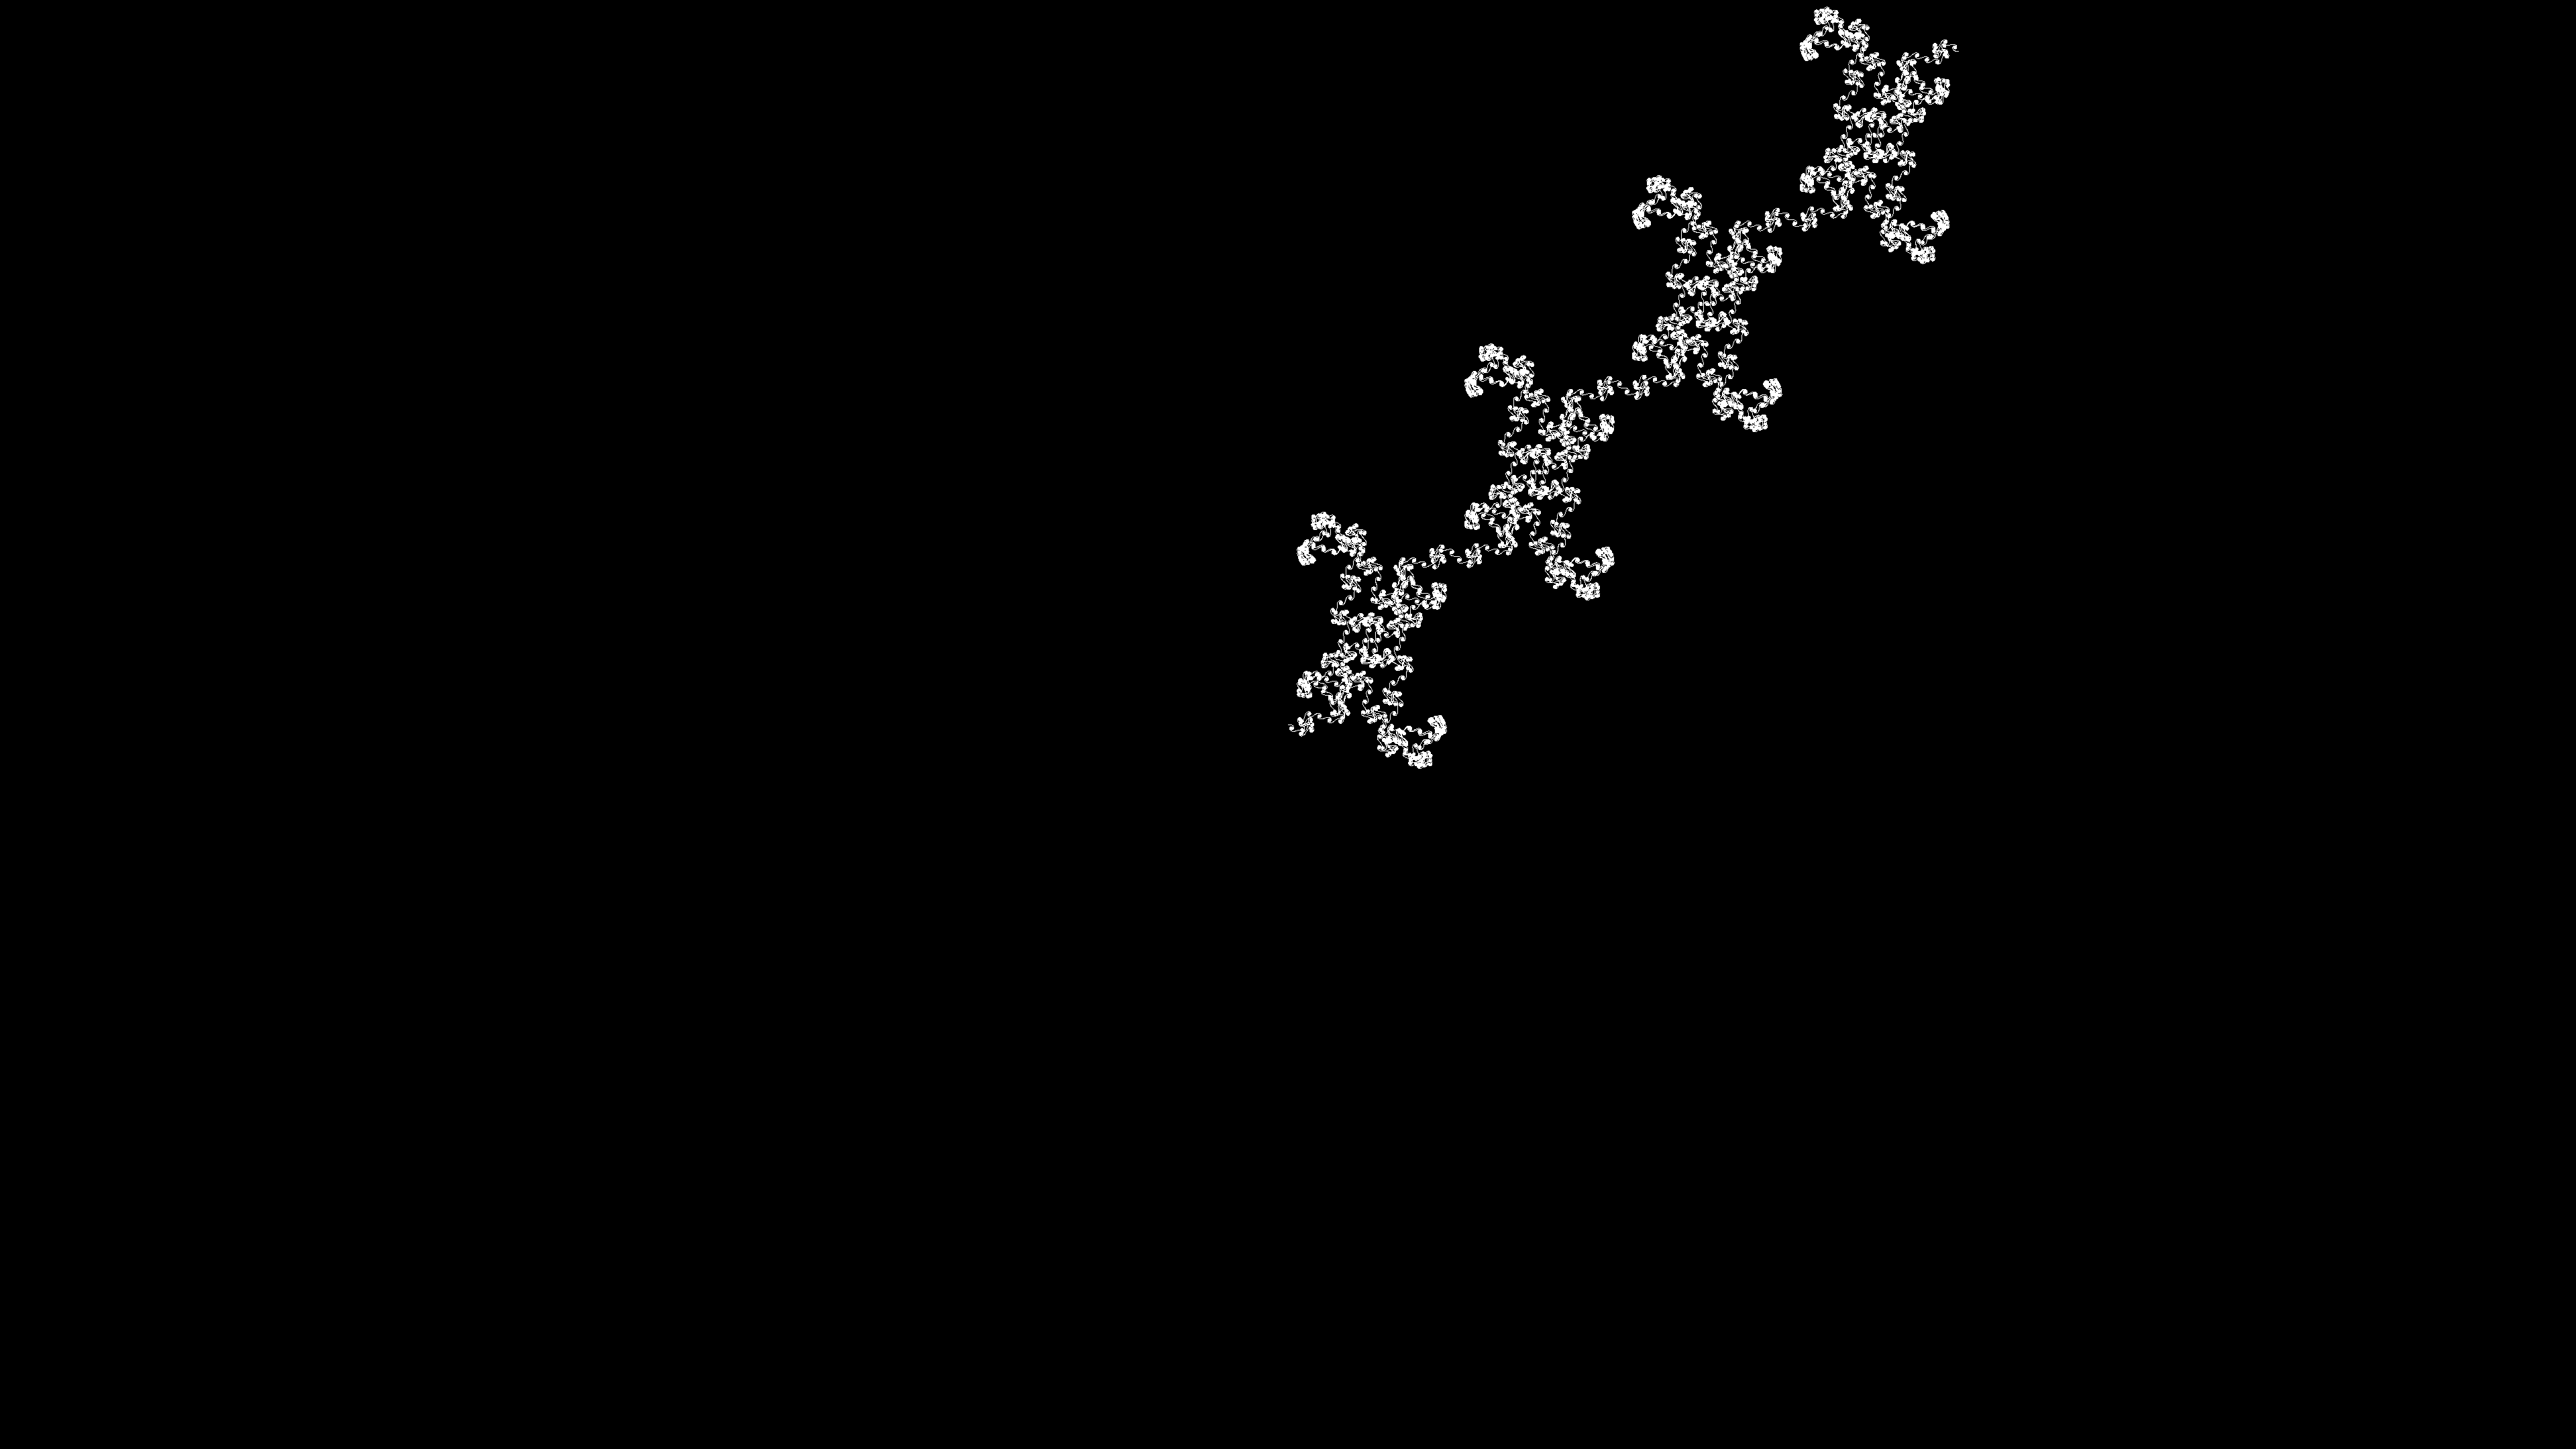
\includegraphics[width=\linewidth]{./stepsplusoneimages/0000000044.png}
    \caption{tf p=499 q=200141 theta=000 89756722.png}
  \end{subfigure}
  \caption{n=042 s=400 s+1=401}
  \label{fig:n=042}
\end{figure}
\begin{figure}[H]
  \centering
  \begin{subfigure}[t]{0.48\textwidth}
    \centering
    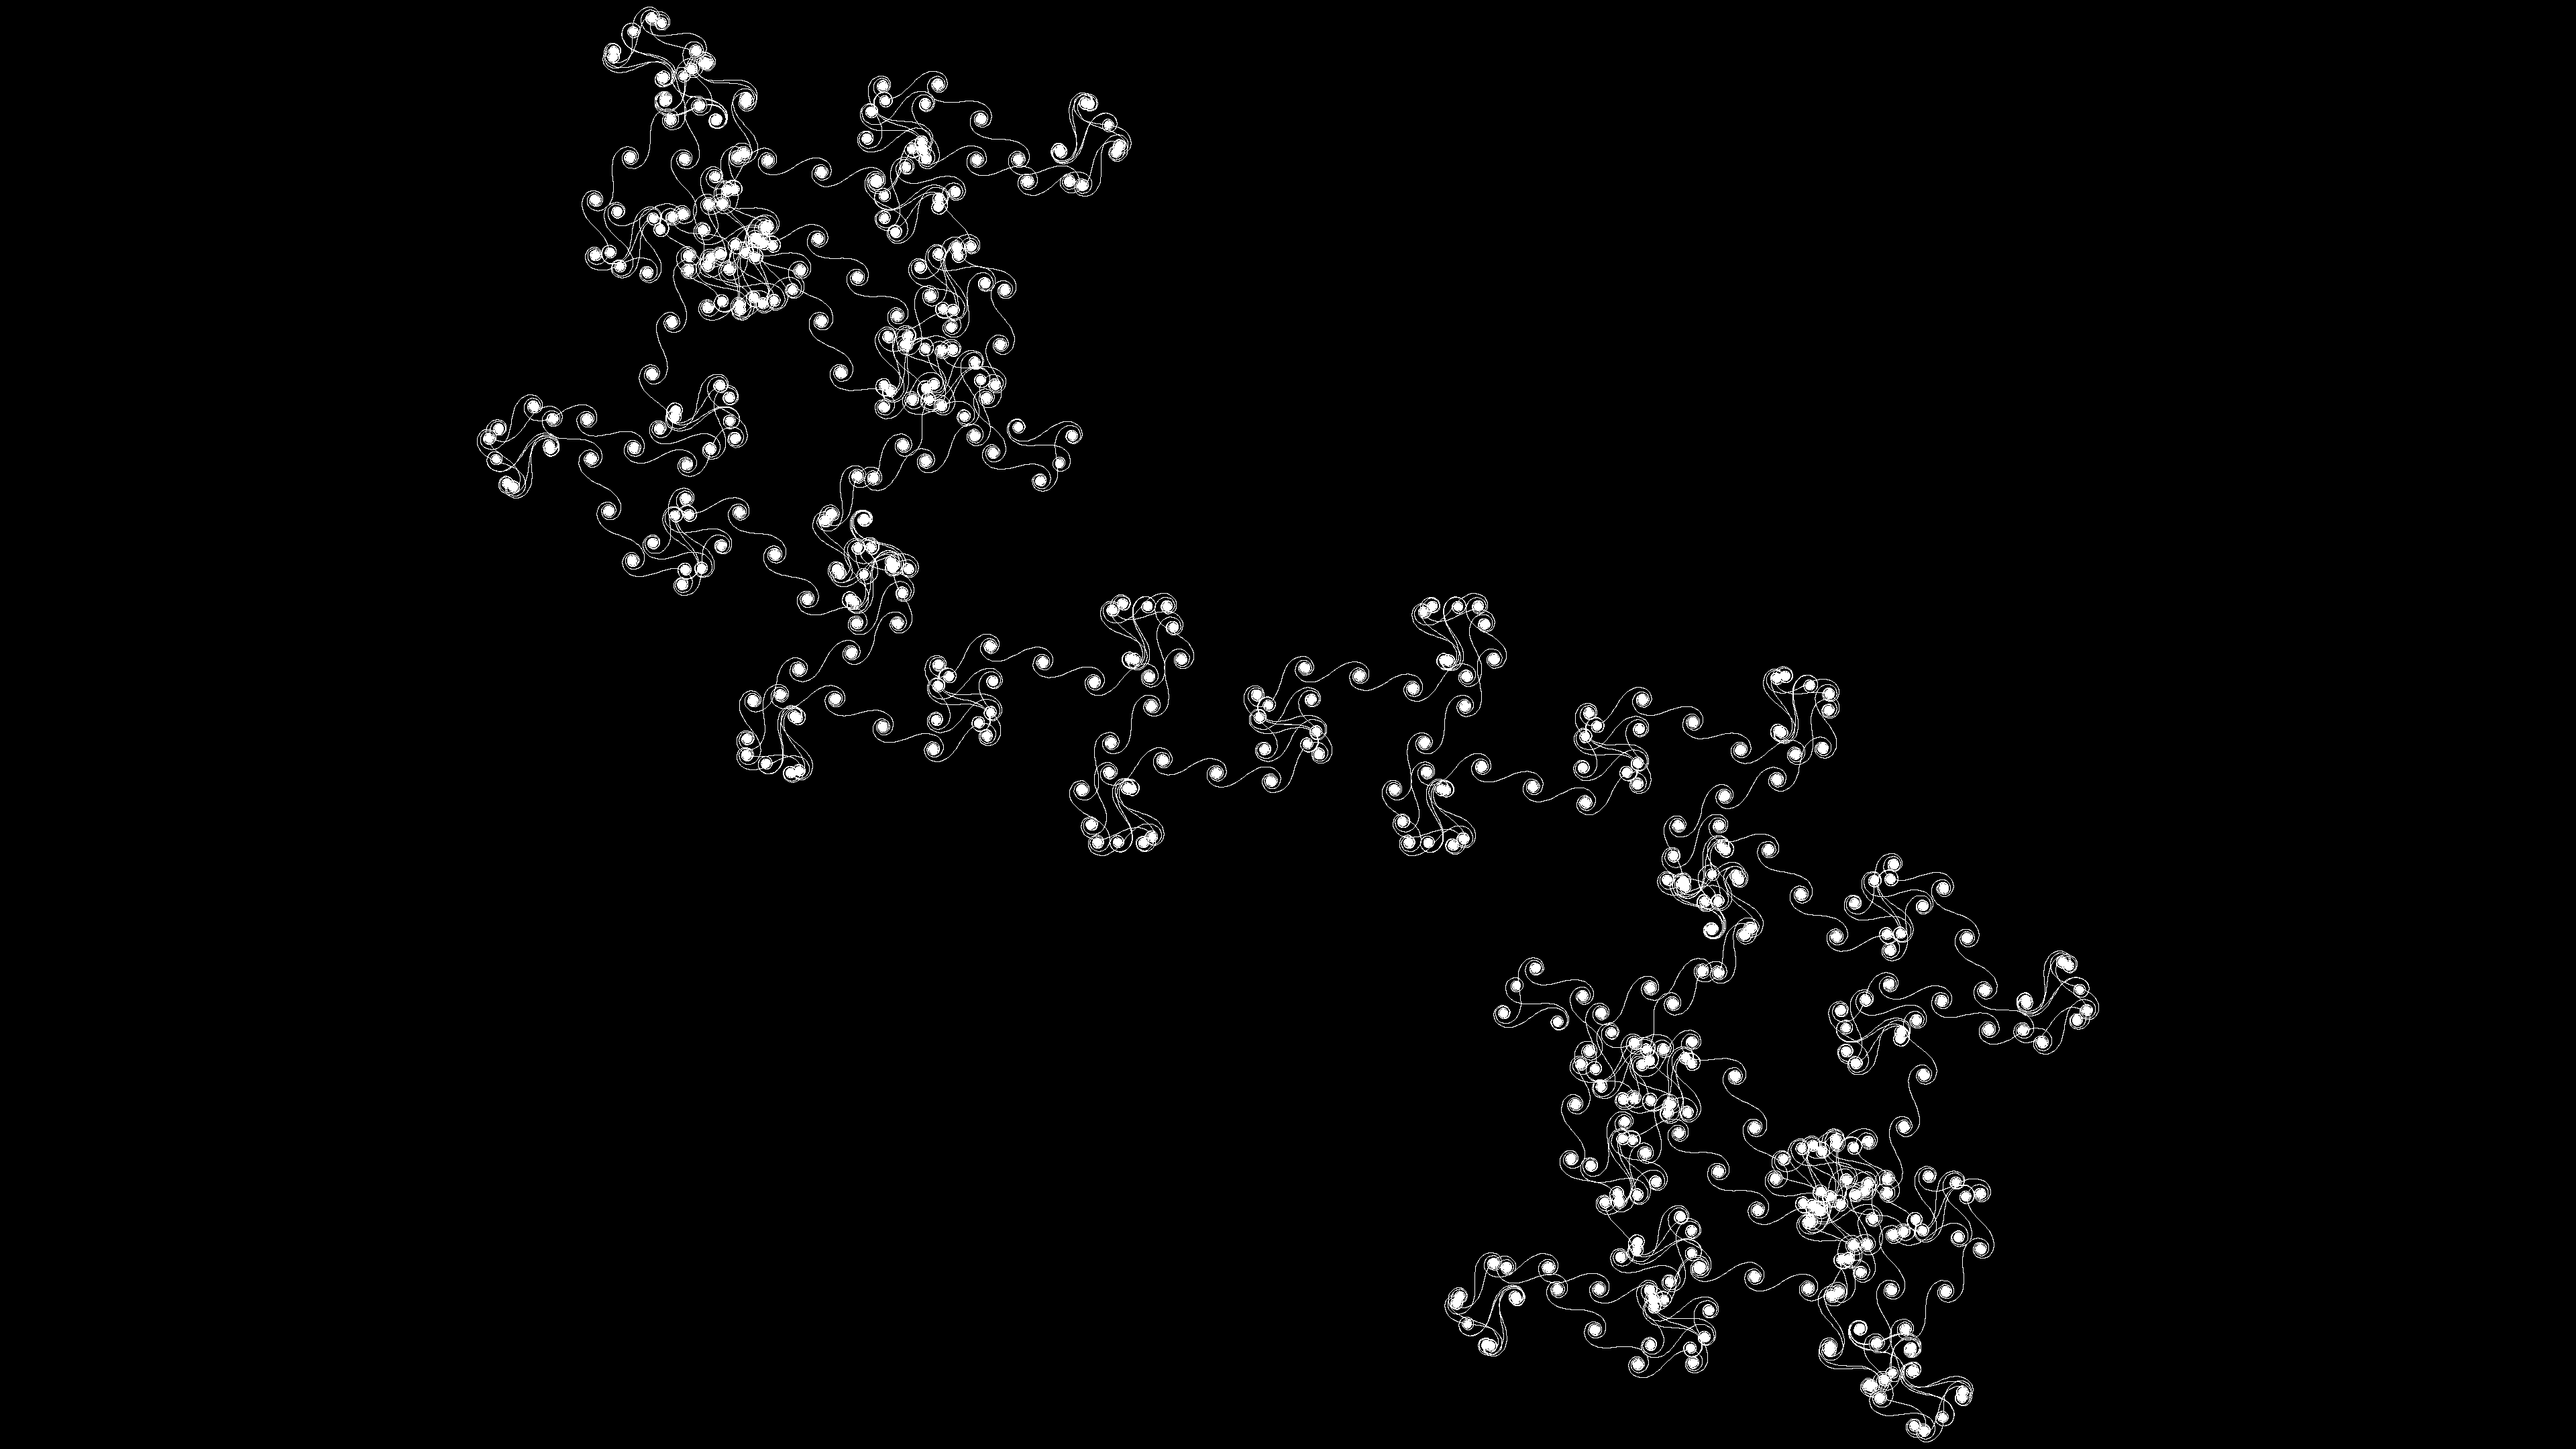
\includegraphics[width=\linewidth]{./stepsplusoneimages/0000000045.png}
    \caption{tf p=499 q=199644 theta=000 89980165.png}
  \end{subfigure}
  \begin{subfigure}[t]{0.48\textwidth}
    \centering
    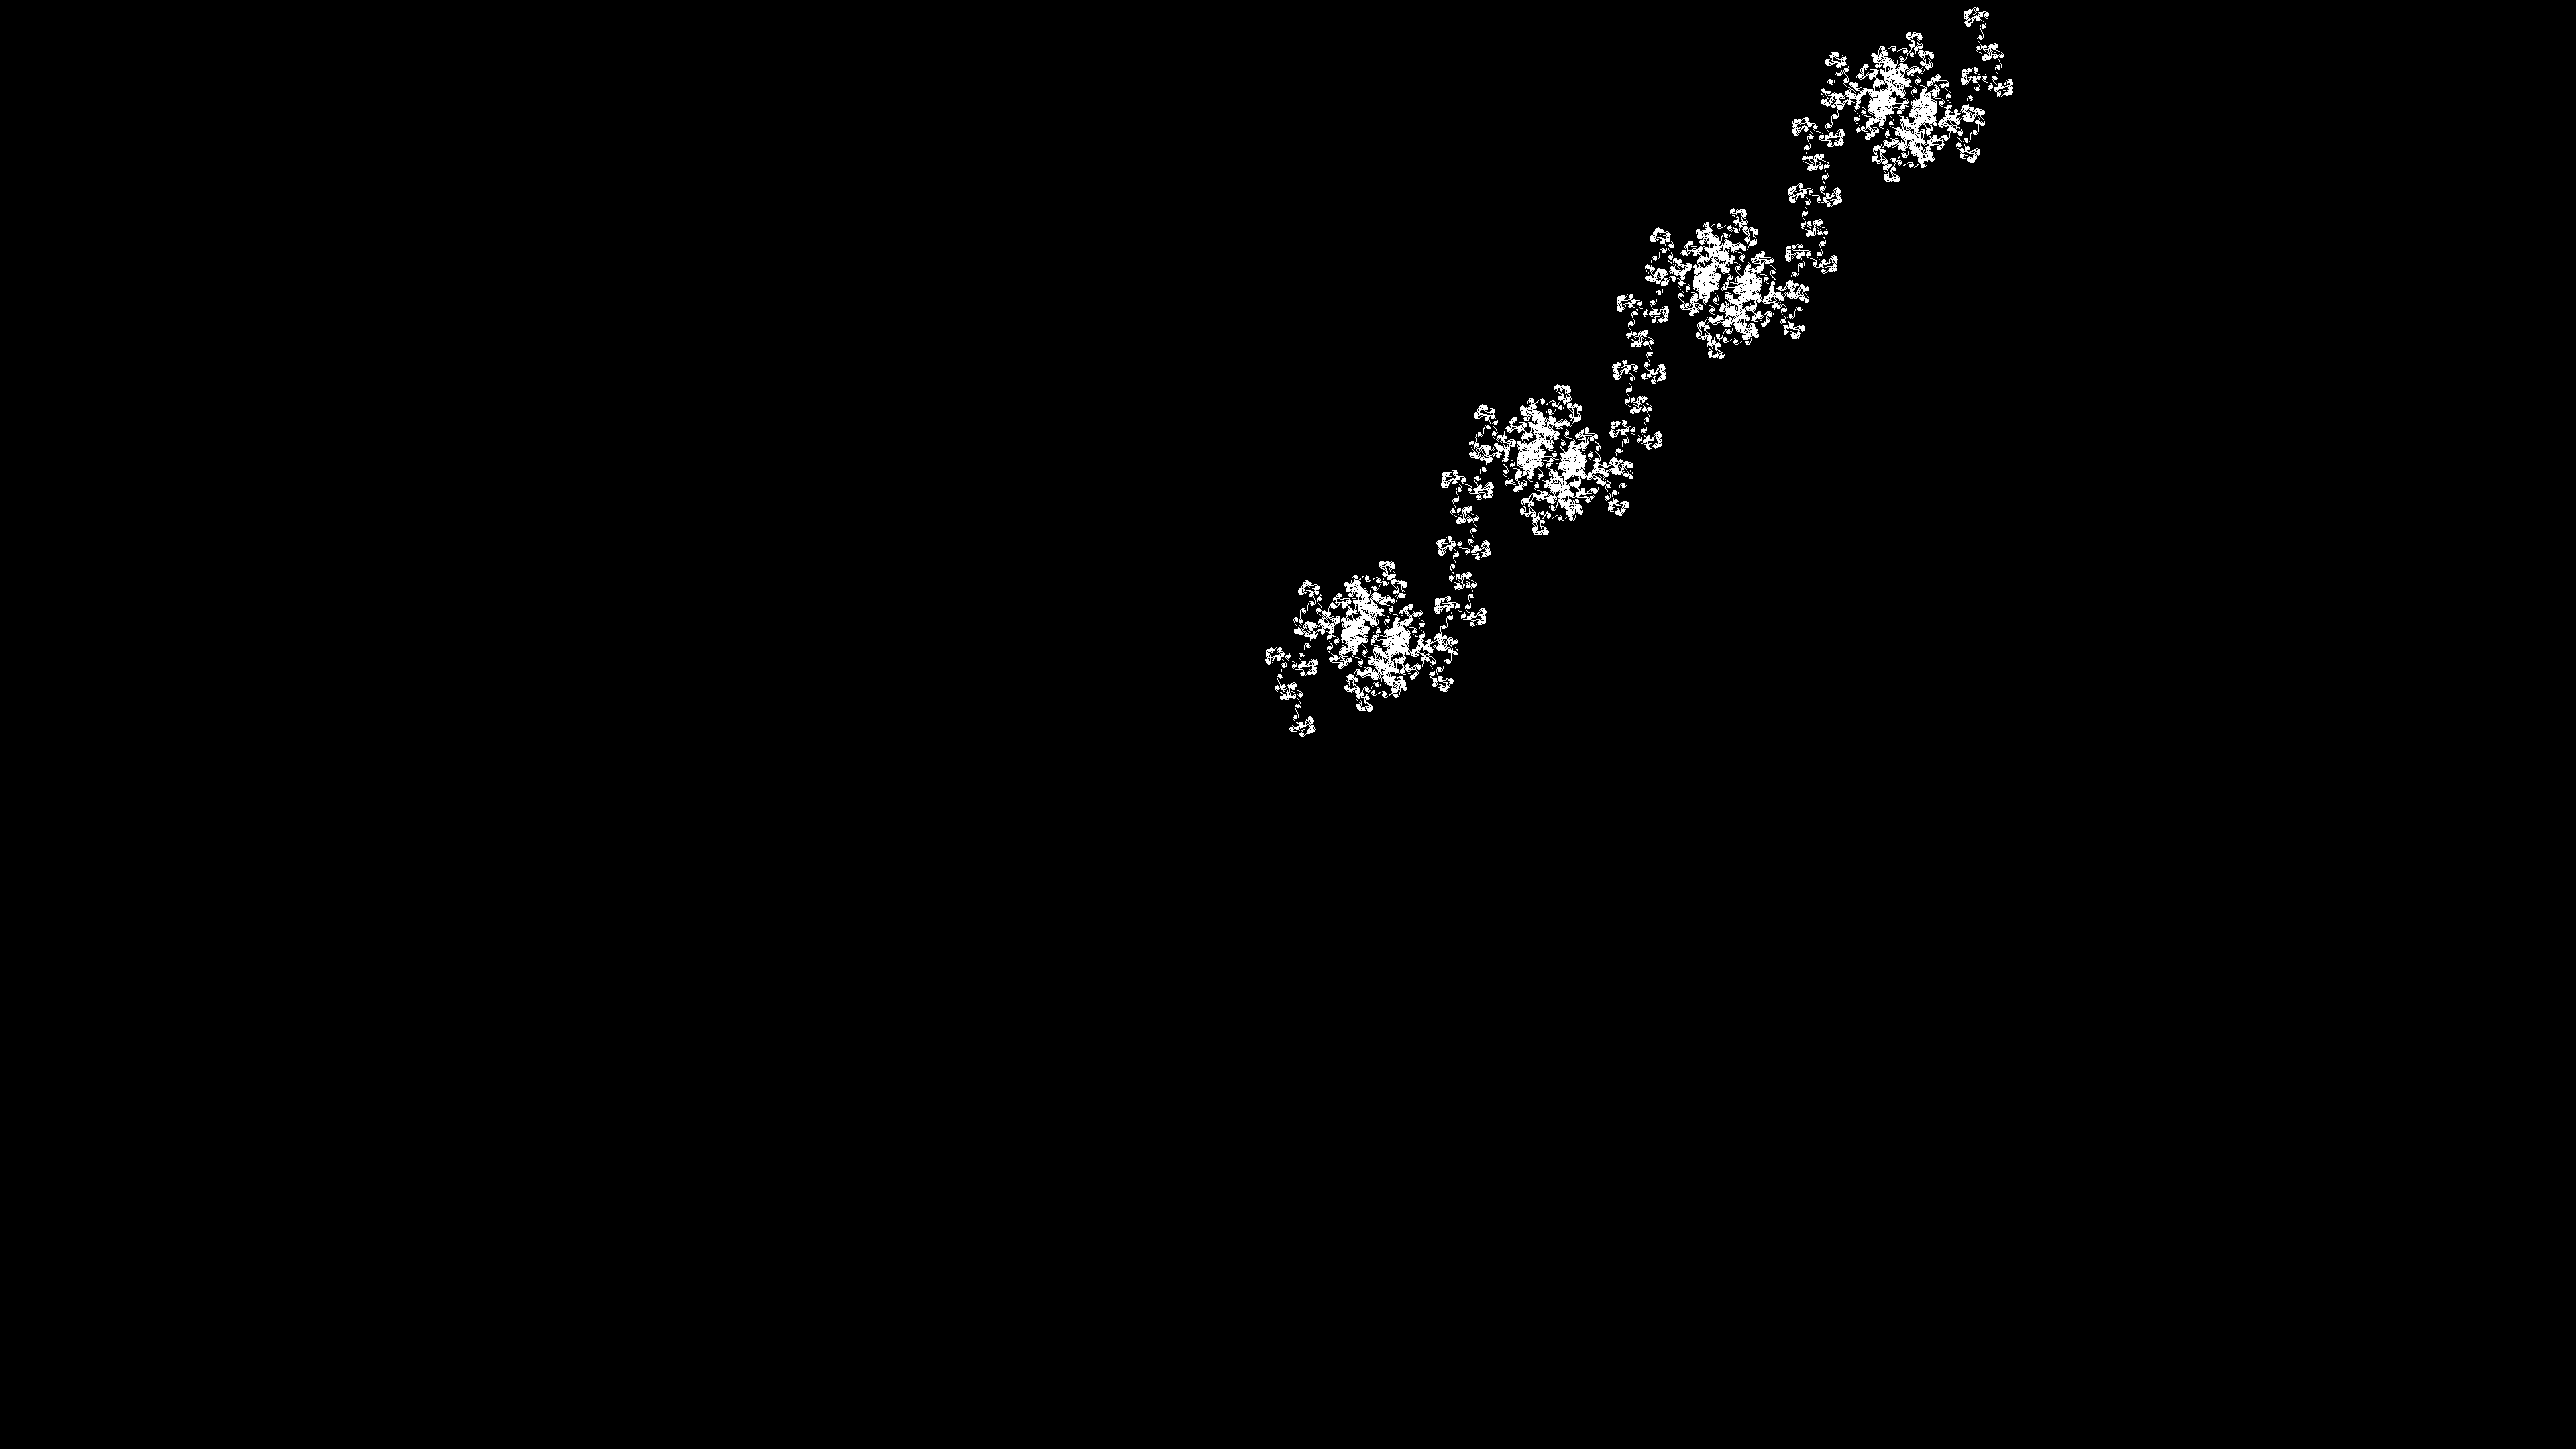
\includegraphics[width=\linewidth]{./stepsplusoneimages/0000000046.png}
    \caption{tf p=499 q=200143 theta=000 89755825.png}
  \end{subfigure}
  \caption{n=044 s=400 s+1=401}
  \label{fig:n=044}
\end{figure}
\begin{figure}[H]
  \centering
  \begin{subfigure}[t]{0.48\textwidth}
    \centering
    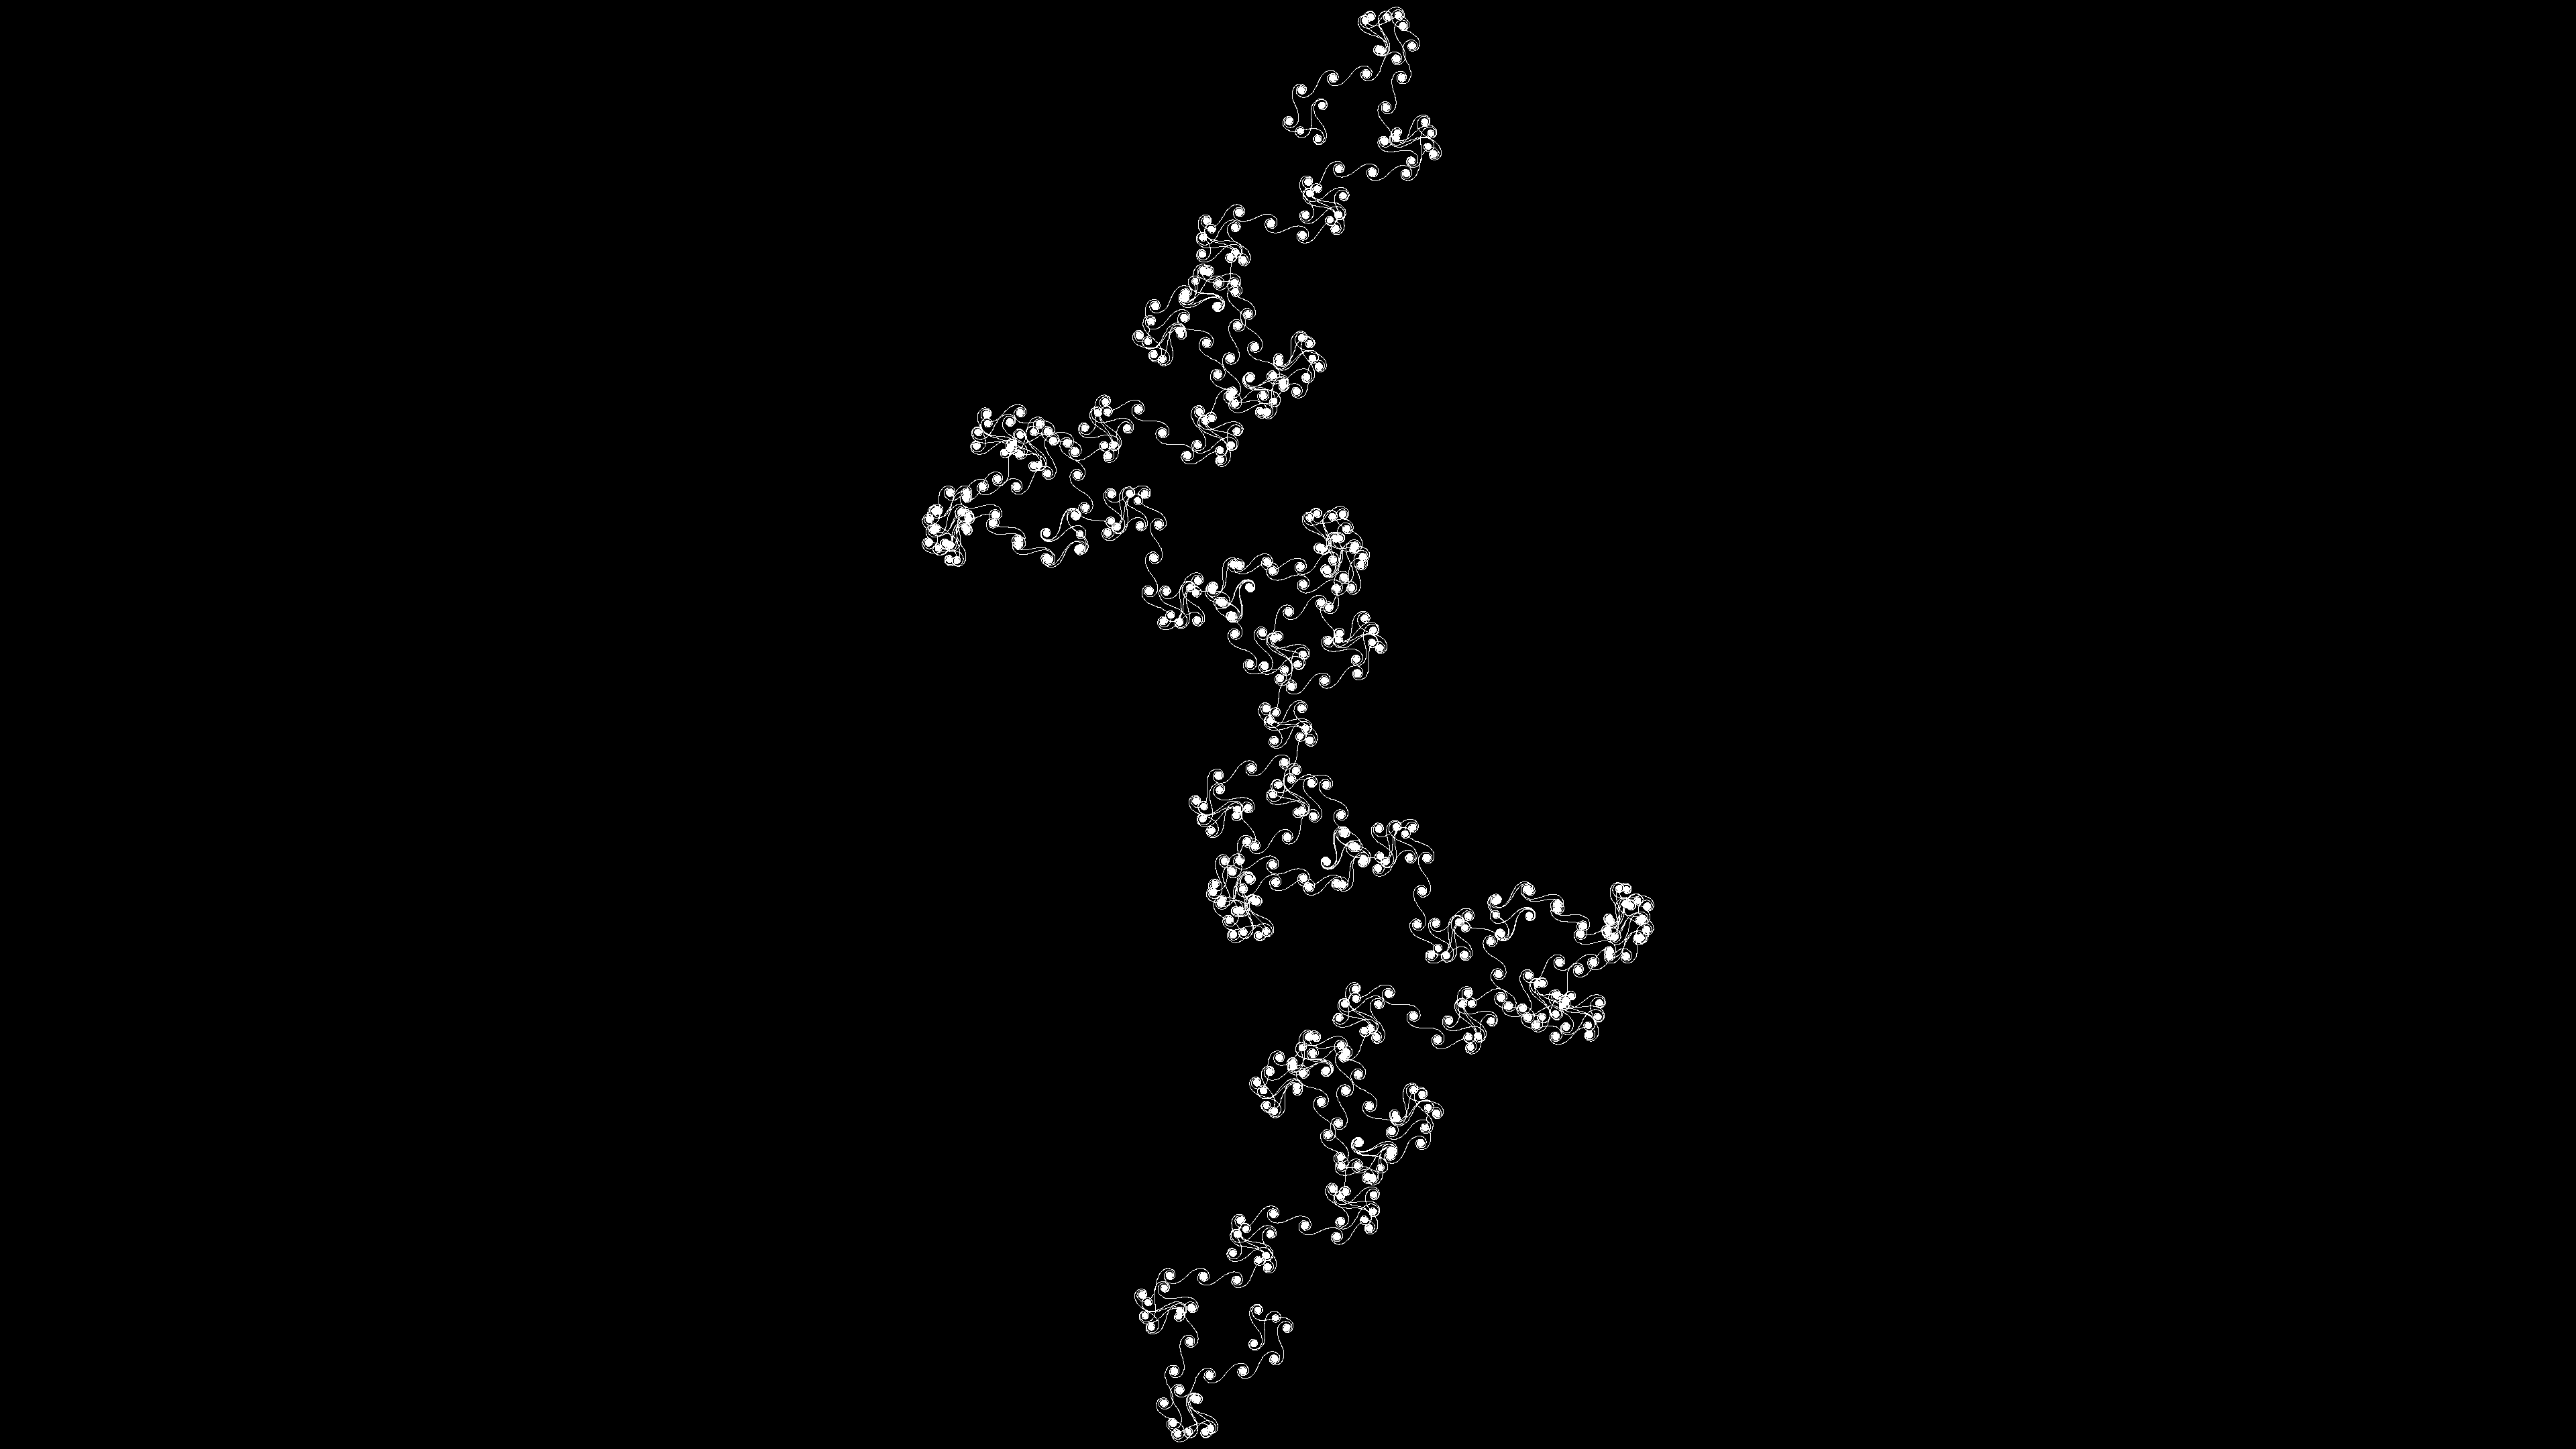
\includegraphics[width=\linewidth]{./stepsplusoneimages/0000000047.png}
    \caption{tf p=499 q=199646 theta=000 89979263.png}
  \end{subfigure}
  \begin{subfigure}[t]{0.48\textwidth}
    \centering
    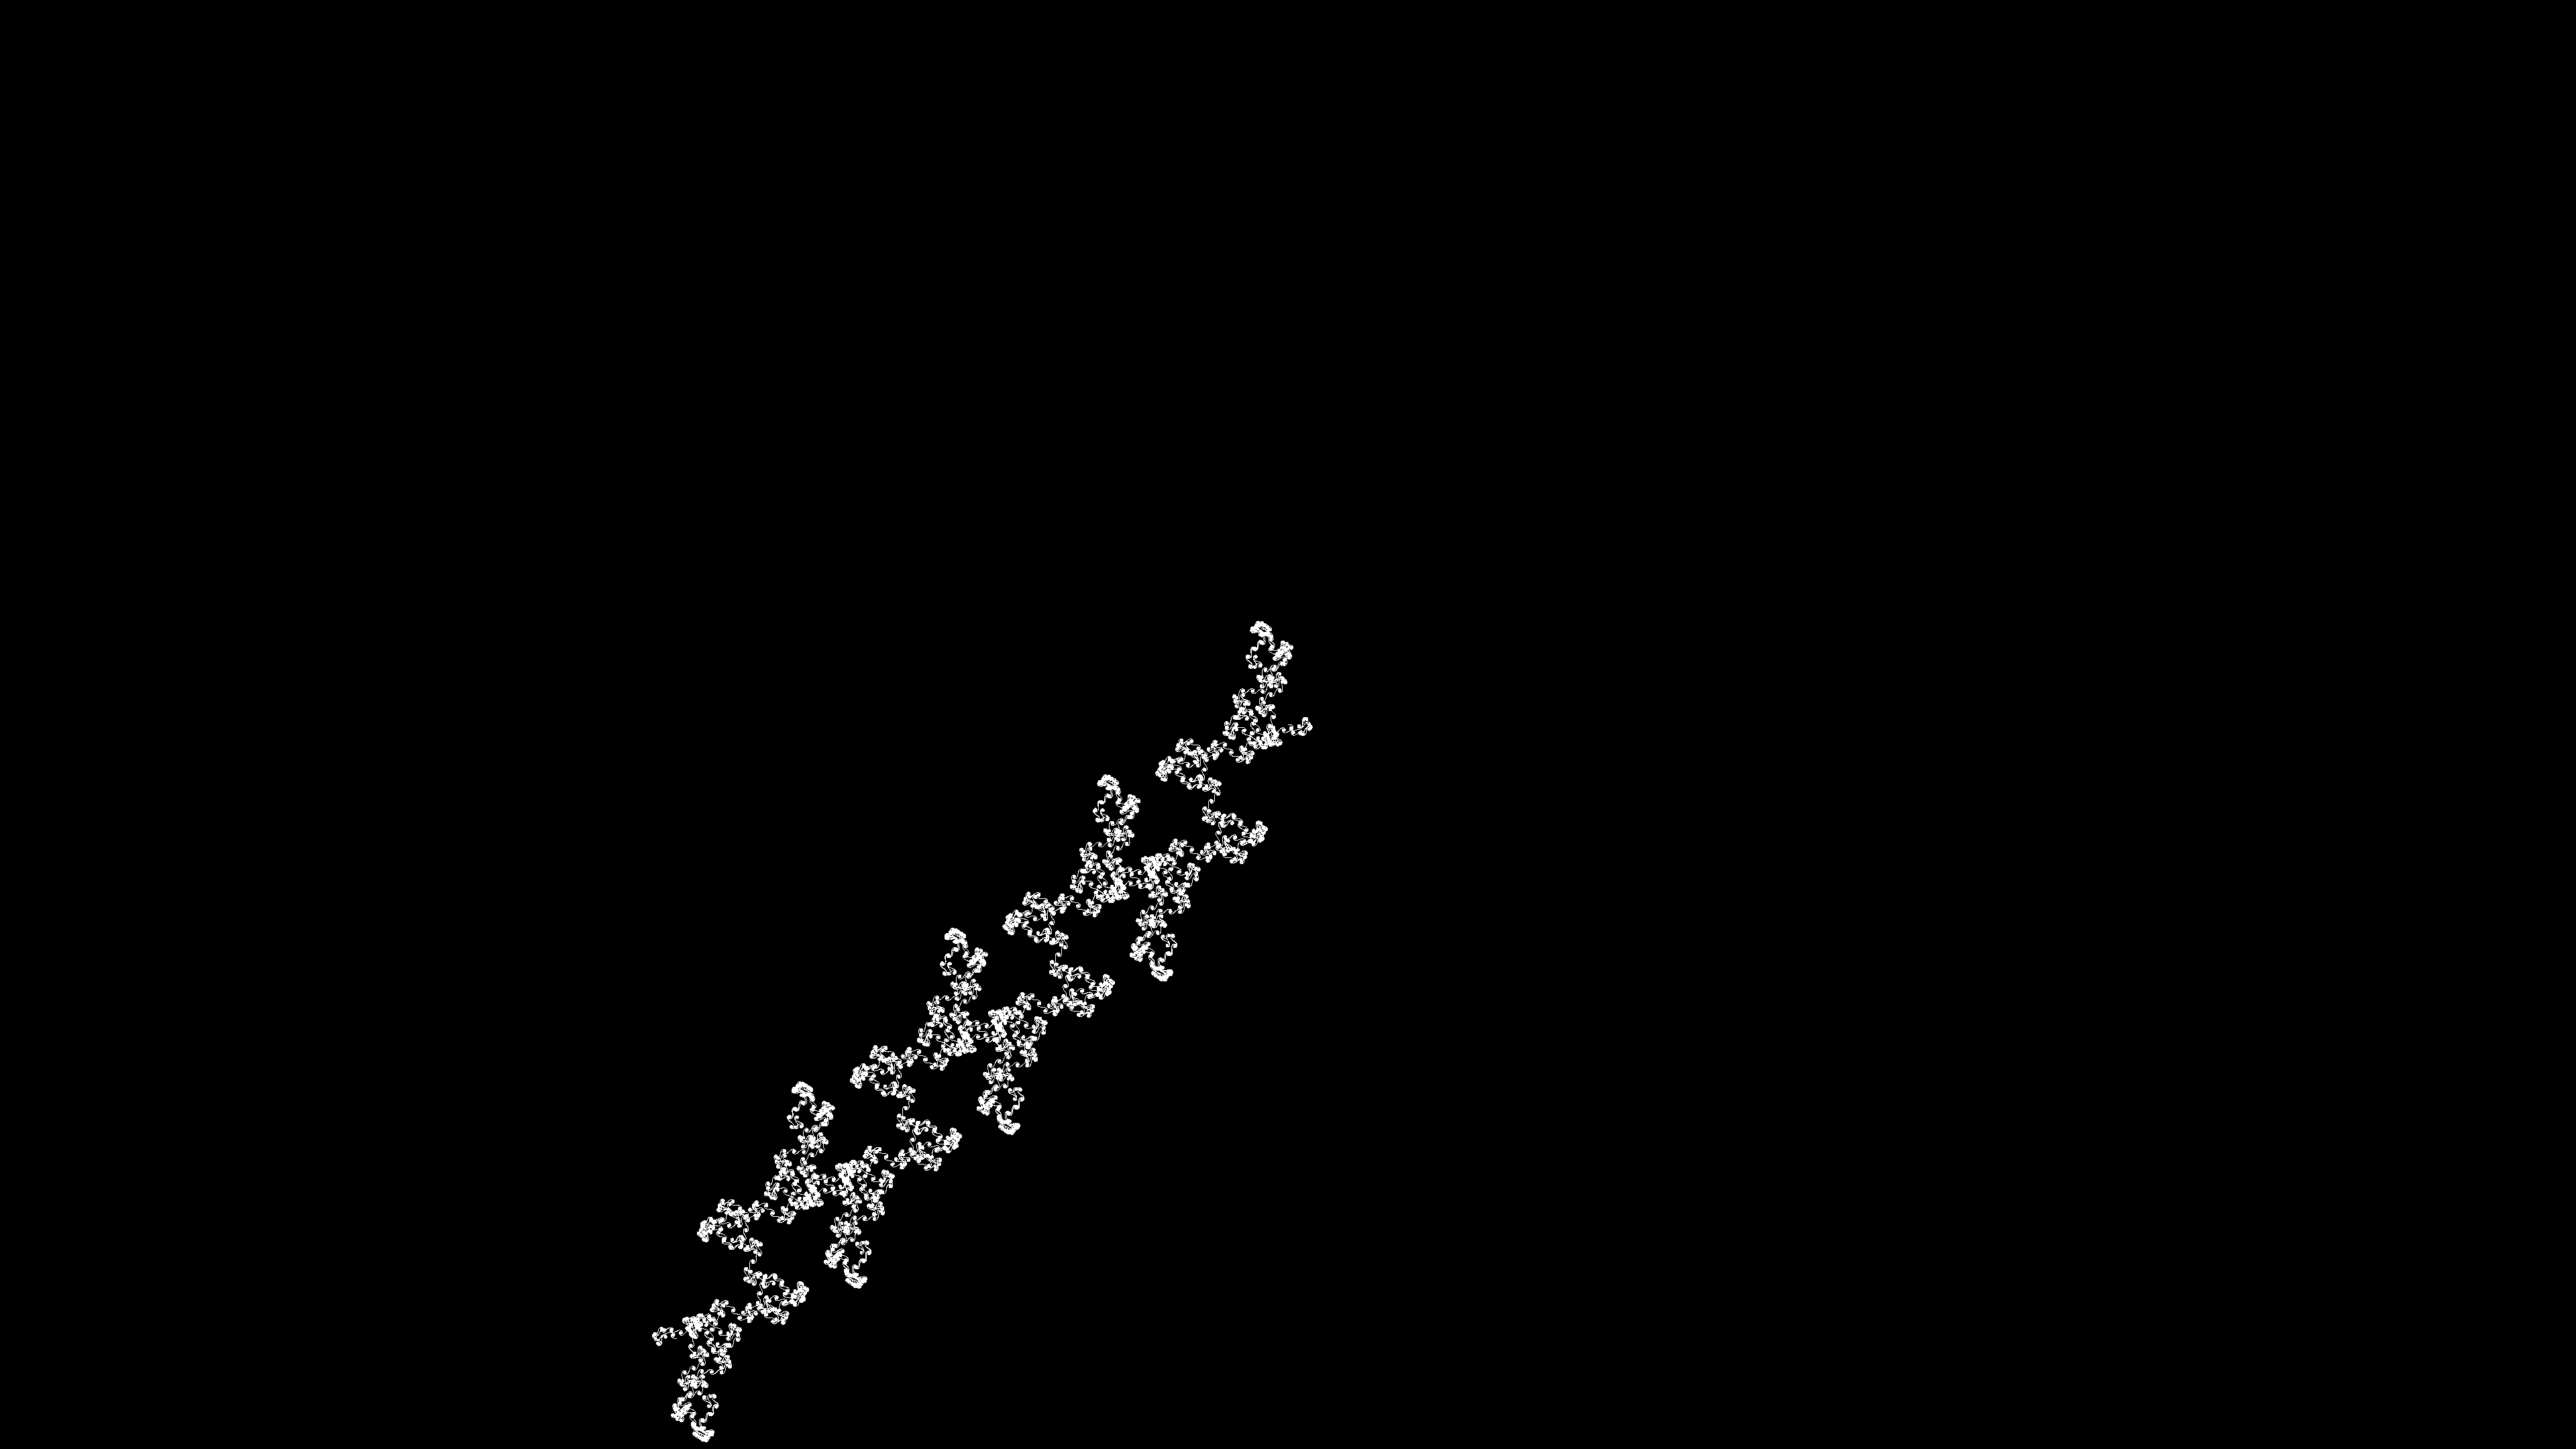
\includegraphics[width=\linewidth]{./stepsplusoneimages/0000000048.png}
    \caption{tf p=499 q=200145 theta=000 89754928.png}
  \end{subfigure}
  \caption{n=046 s=400 s+1=401}
  \label{fig:n=046}
\end{figure}
\begin{figure}[H]
  \centering
  \begin{subfigure}[t]{0.48\textwidth}
    \centering
    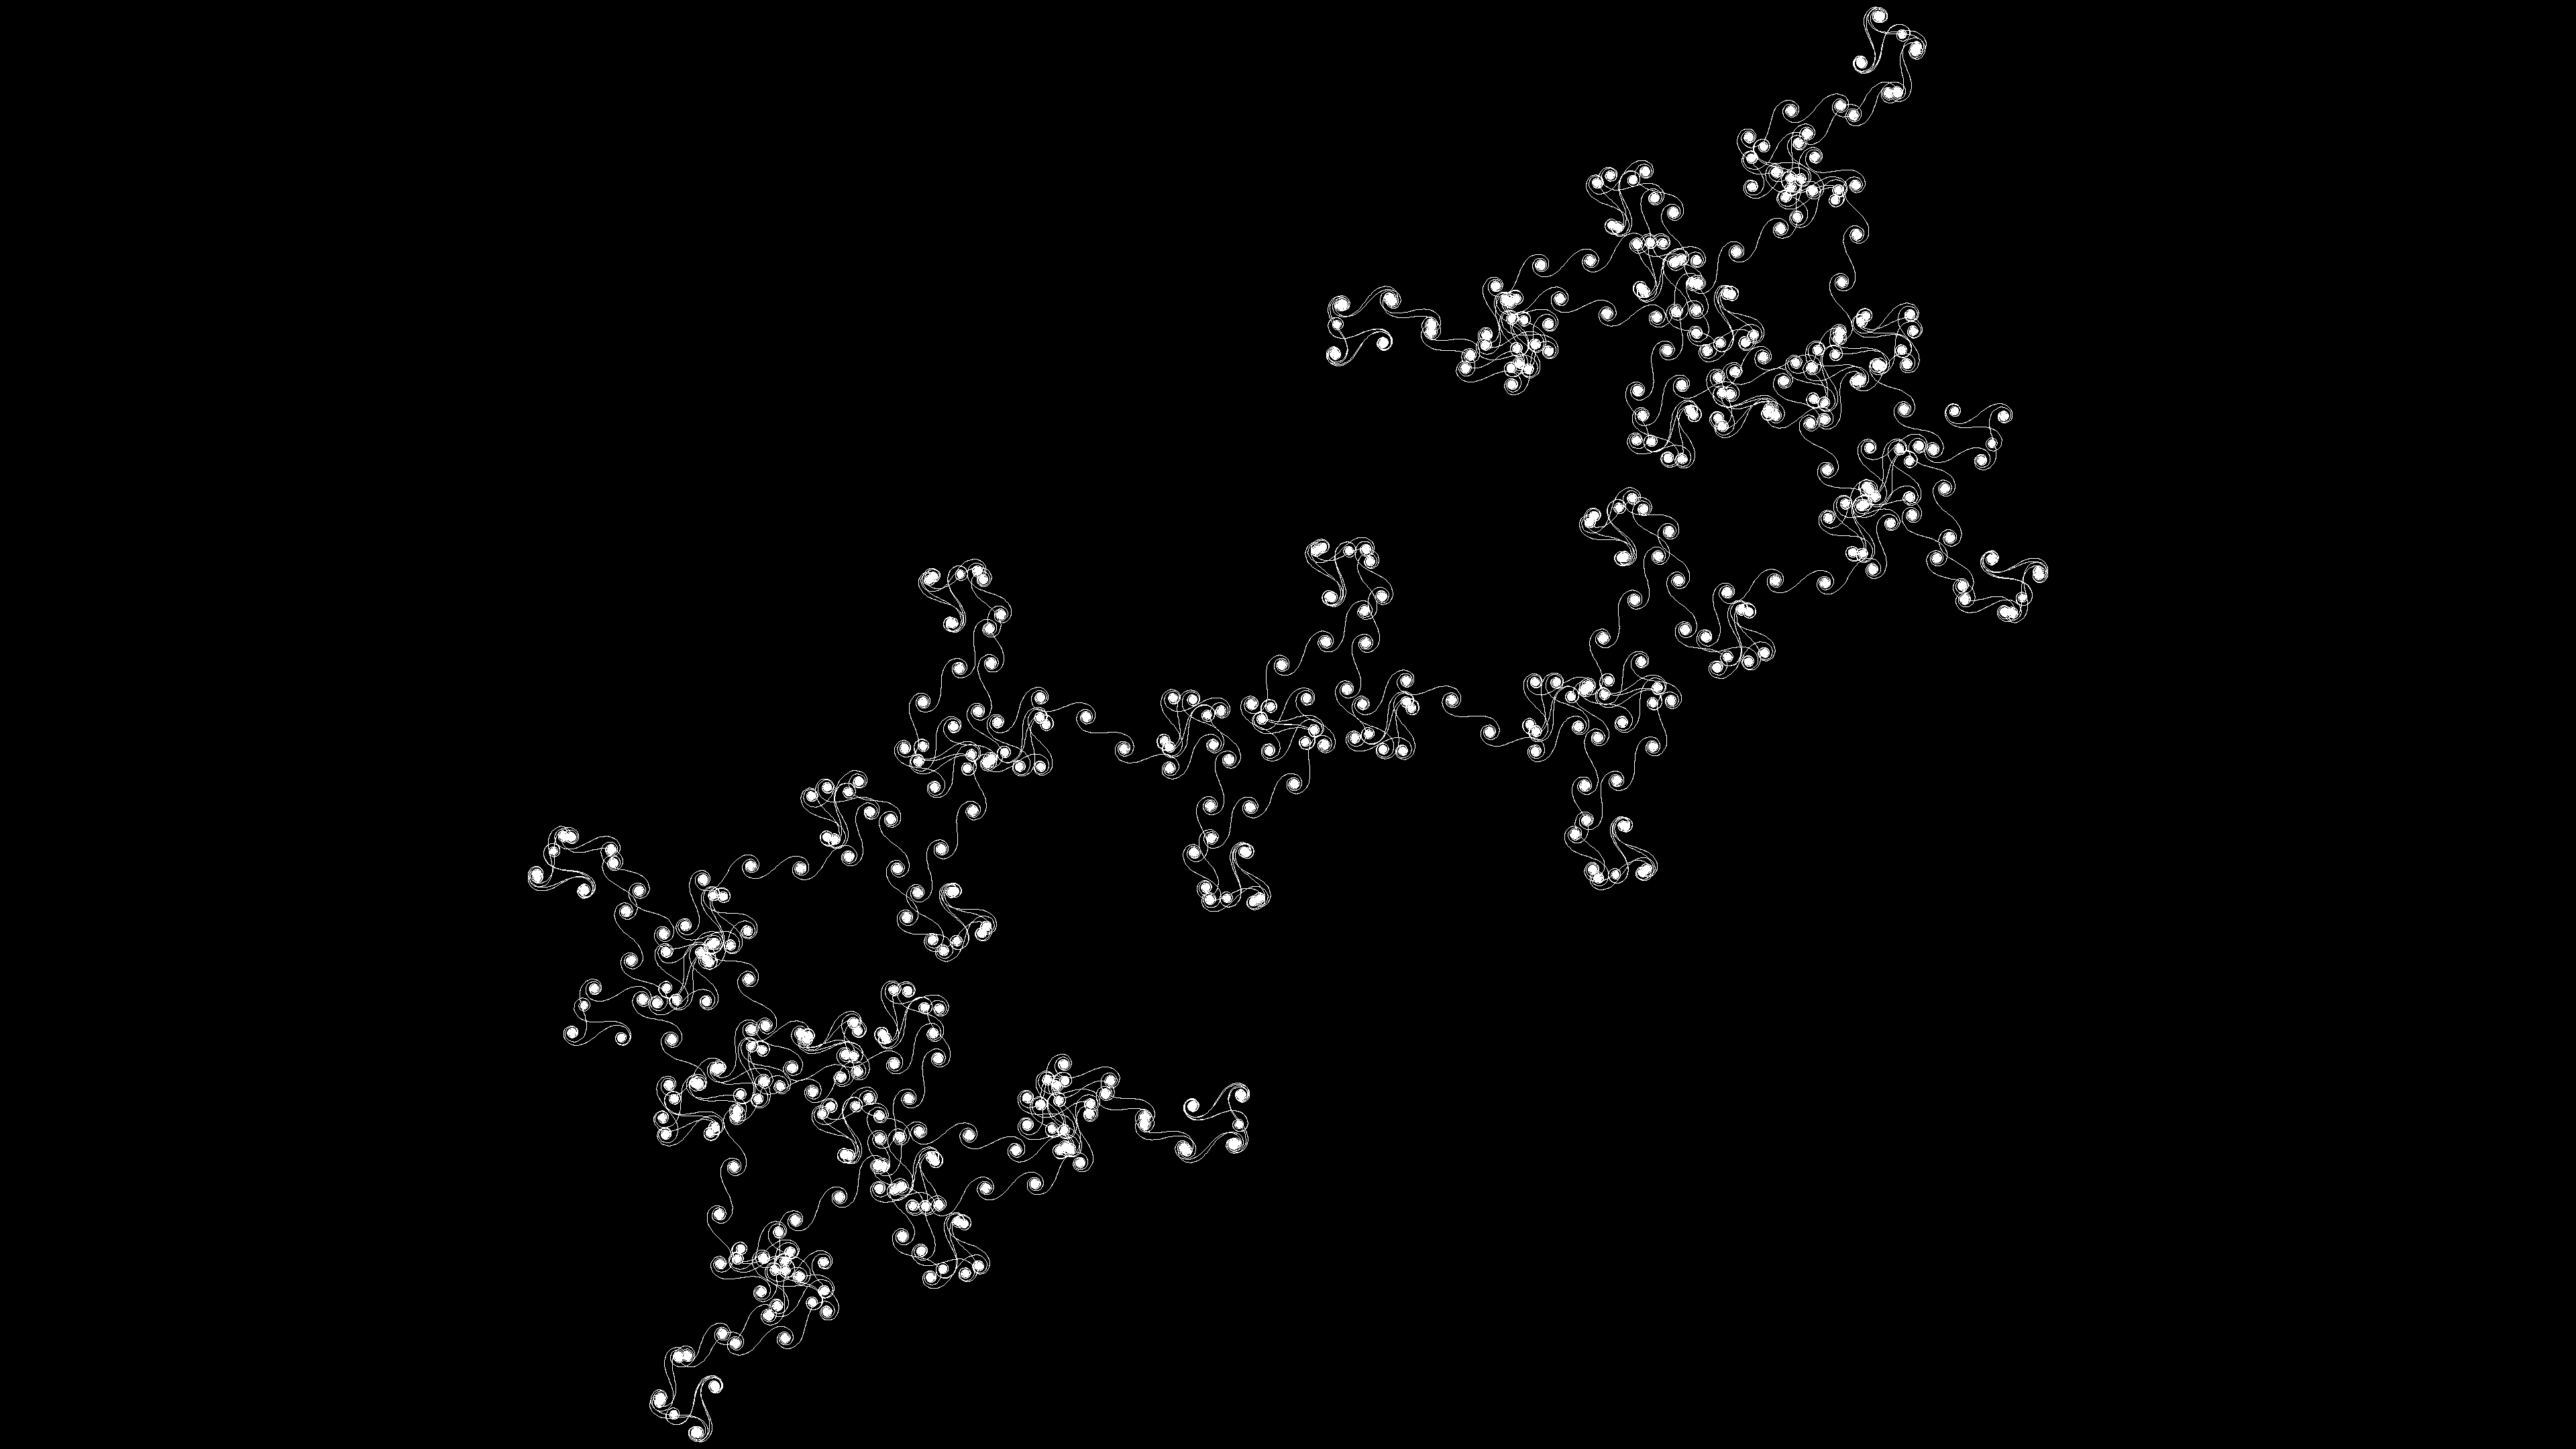
\includegraphics[width=\linewidth]{./stepsplusoneimages/0000000049.png}
    \caption{tf p=499 q=199648 theta=000 89978362.png}
  \end{subfigure}
  \begin{subfigure}[t]{0.48\textwidth}
    \centering
    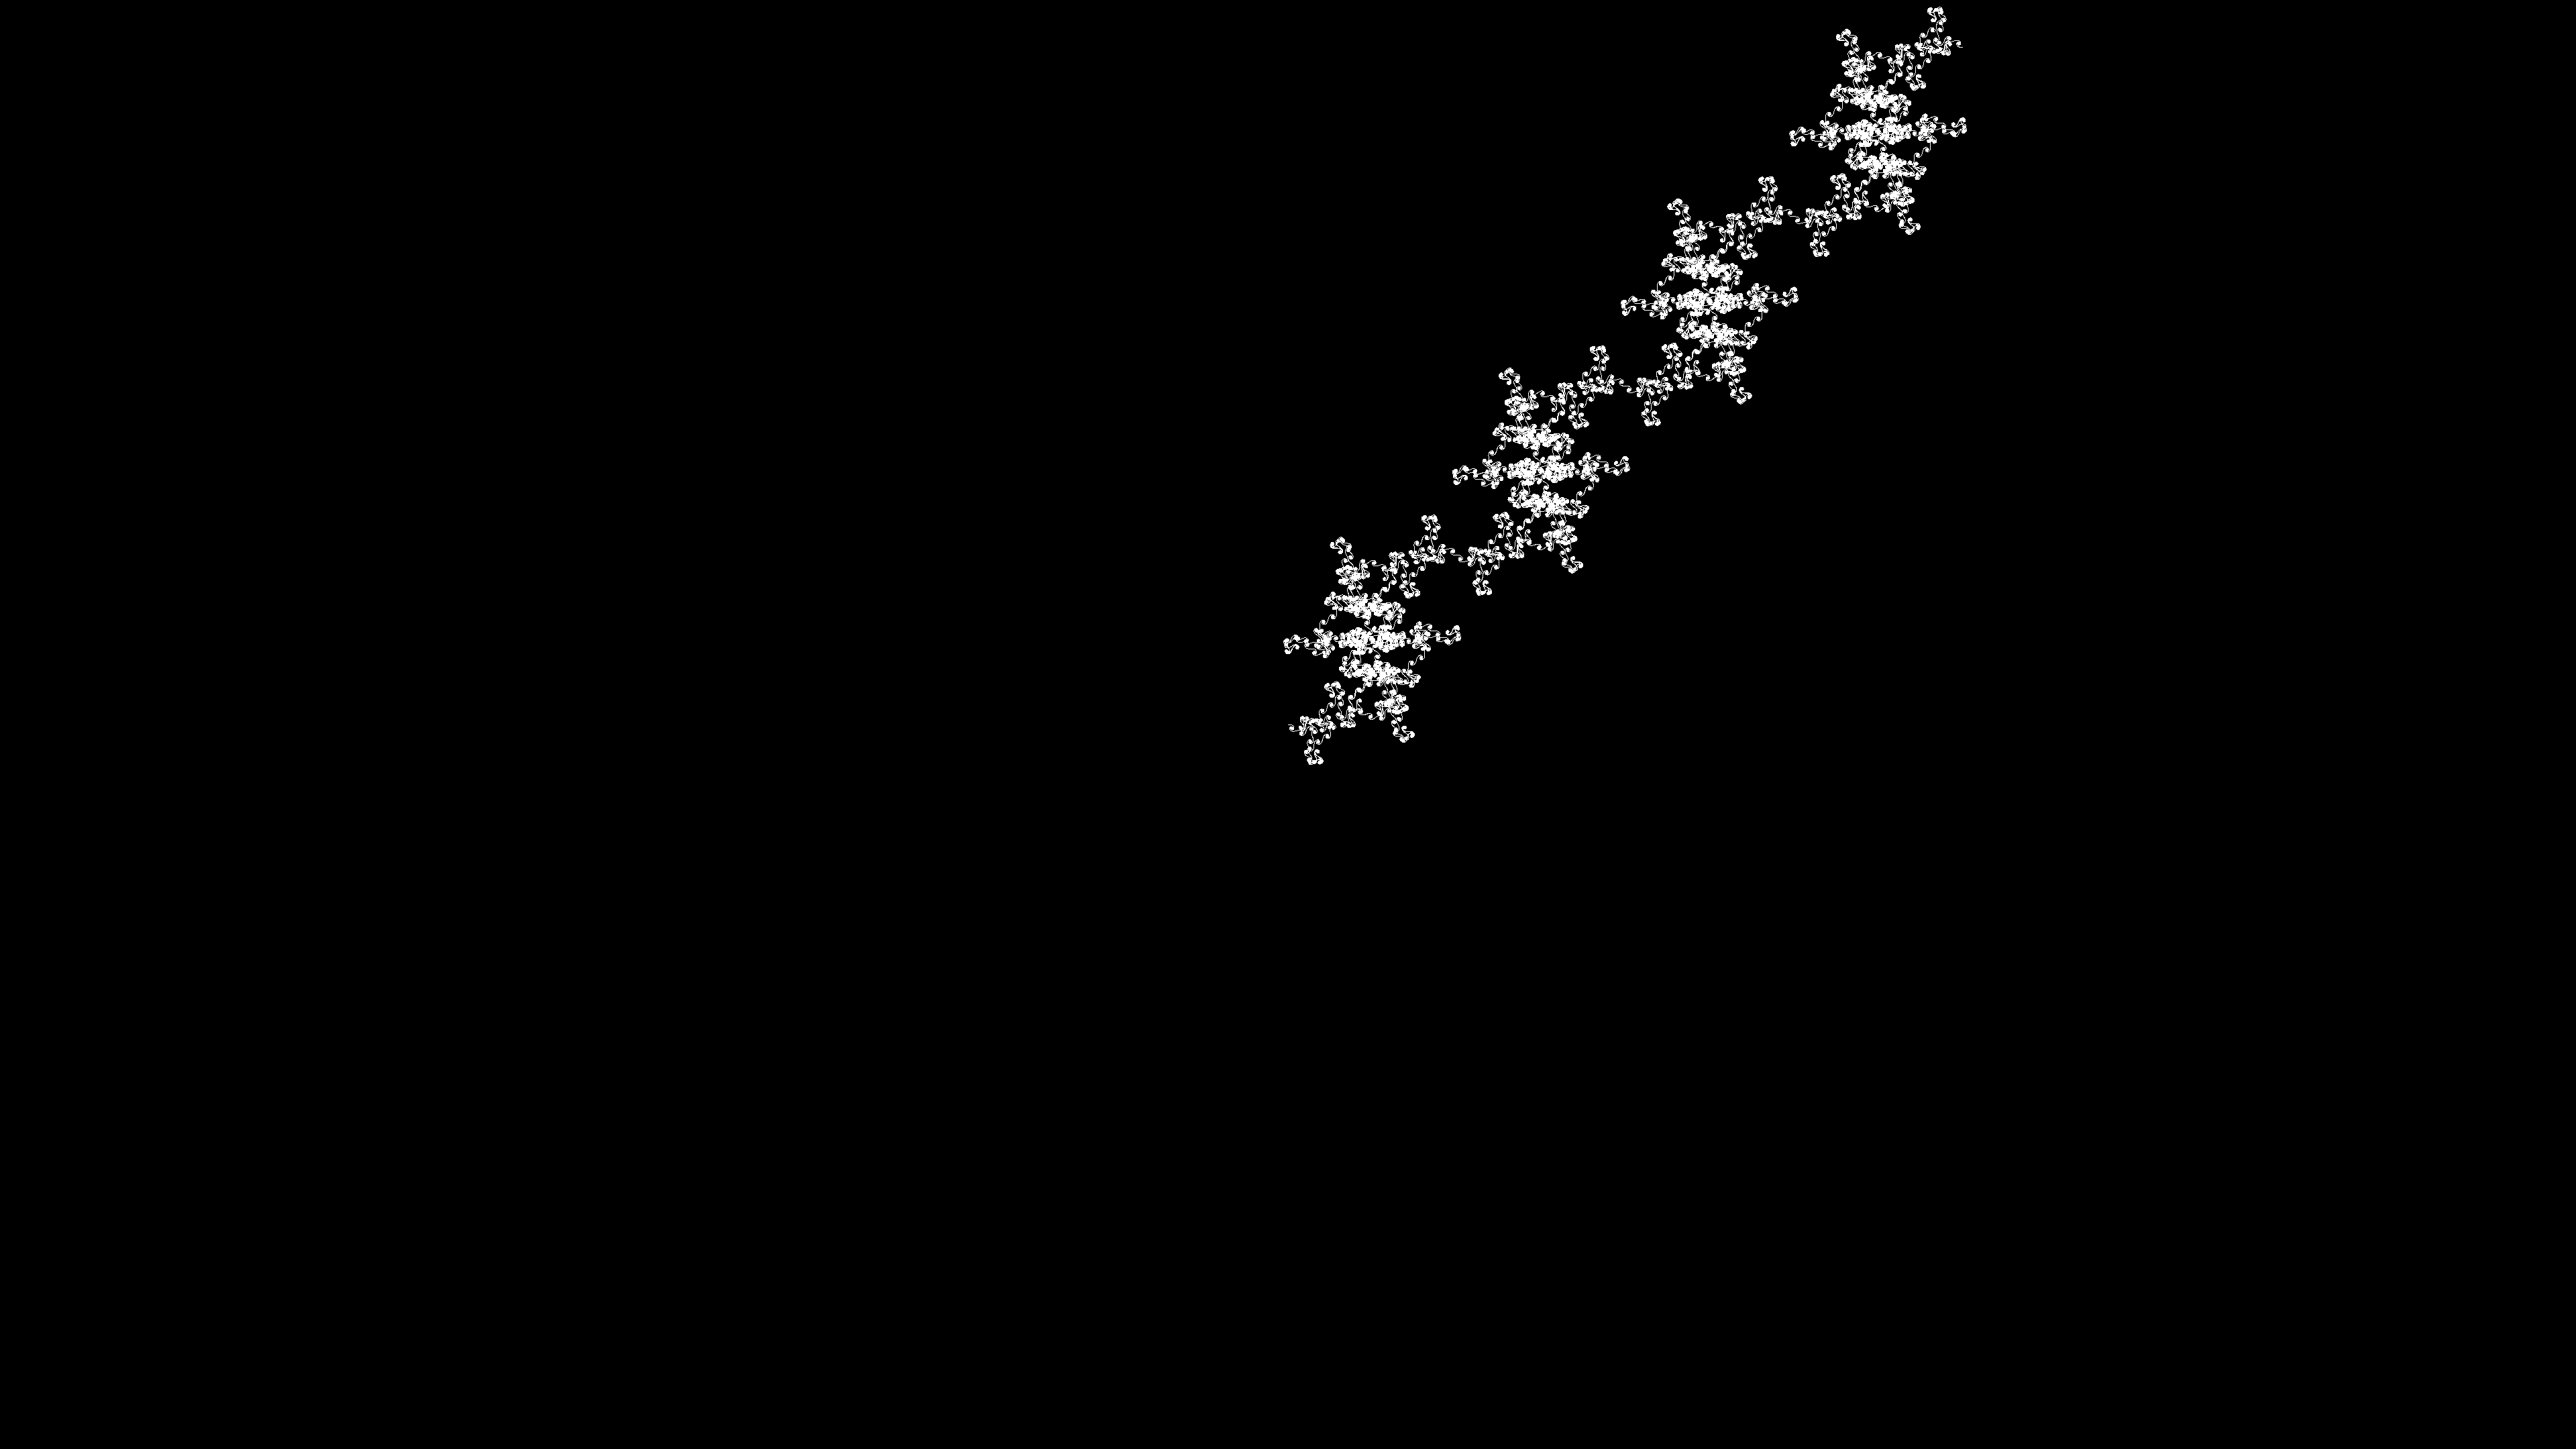
\includegraphics[width=\linewidth]{./stepsplusoneimages/0000000050.png}
    \caption{tf p=499 q=200147 theta=000 89754031.png}
  \end{subfigure}
  \caption{n=048 s=400 s+1=401}
  \label{fig:n=048}
\end{figure}
\begin{figure}[H]
  \centering
  \begin{subfigure}[t]{0.48\textwidth}
    \centering
    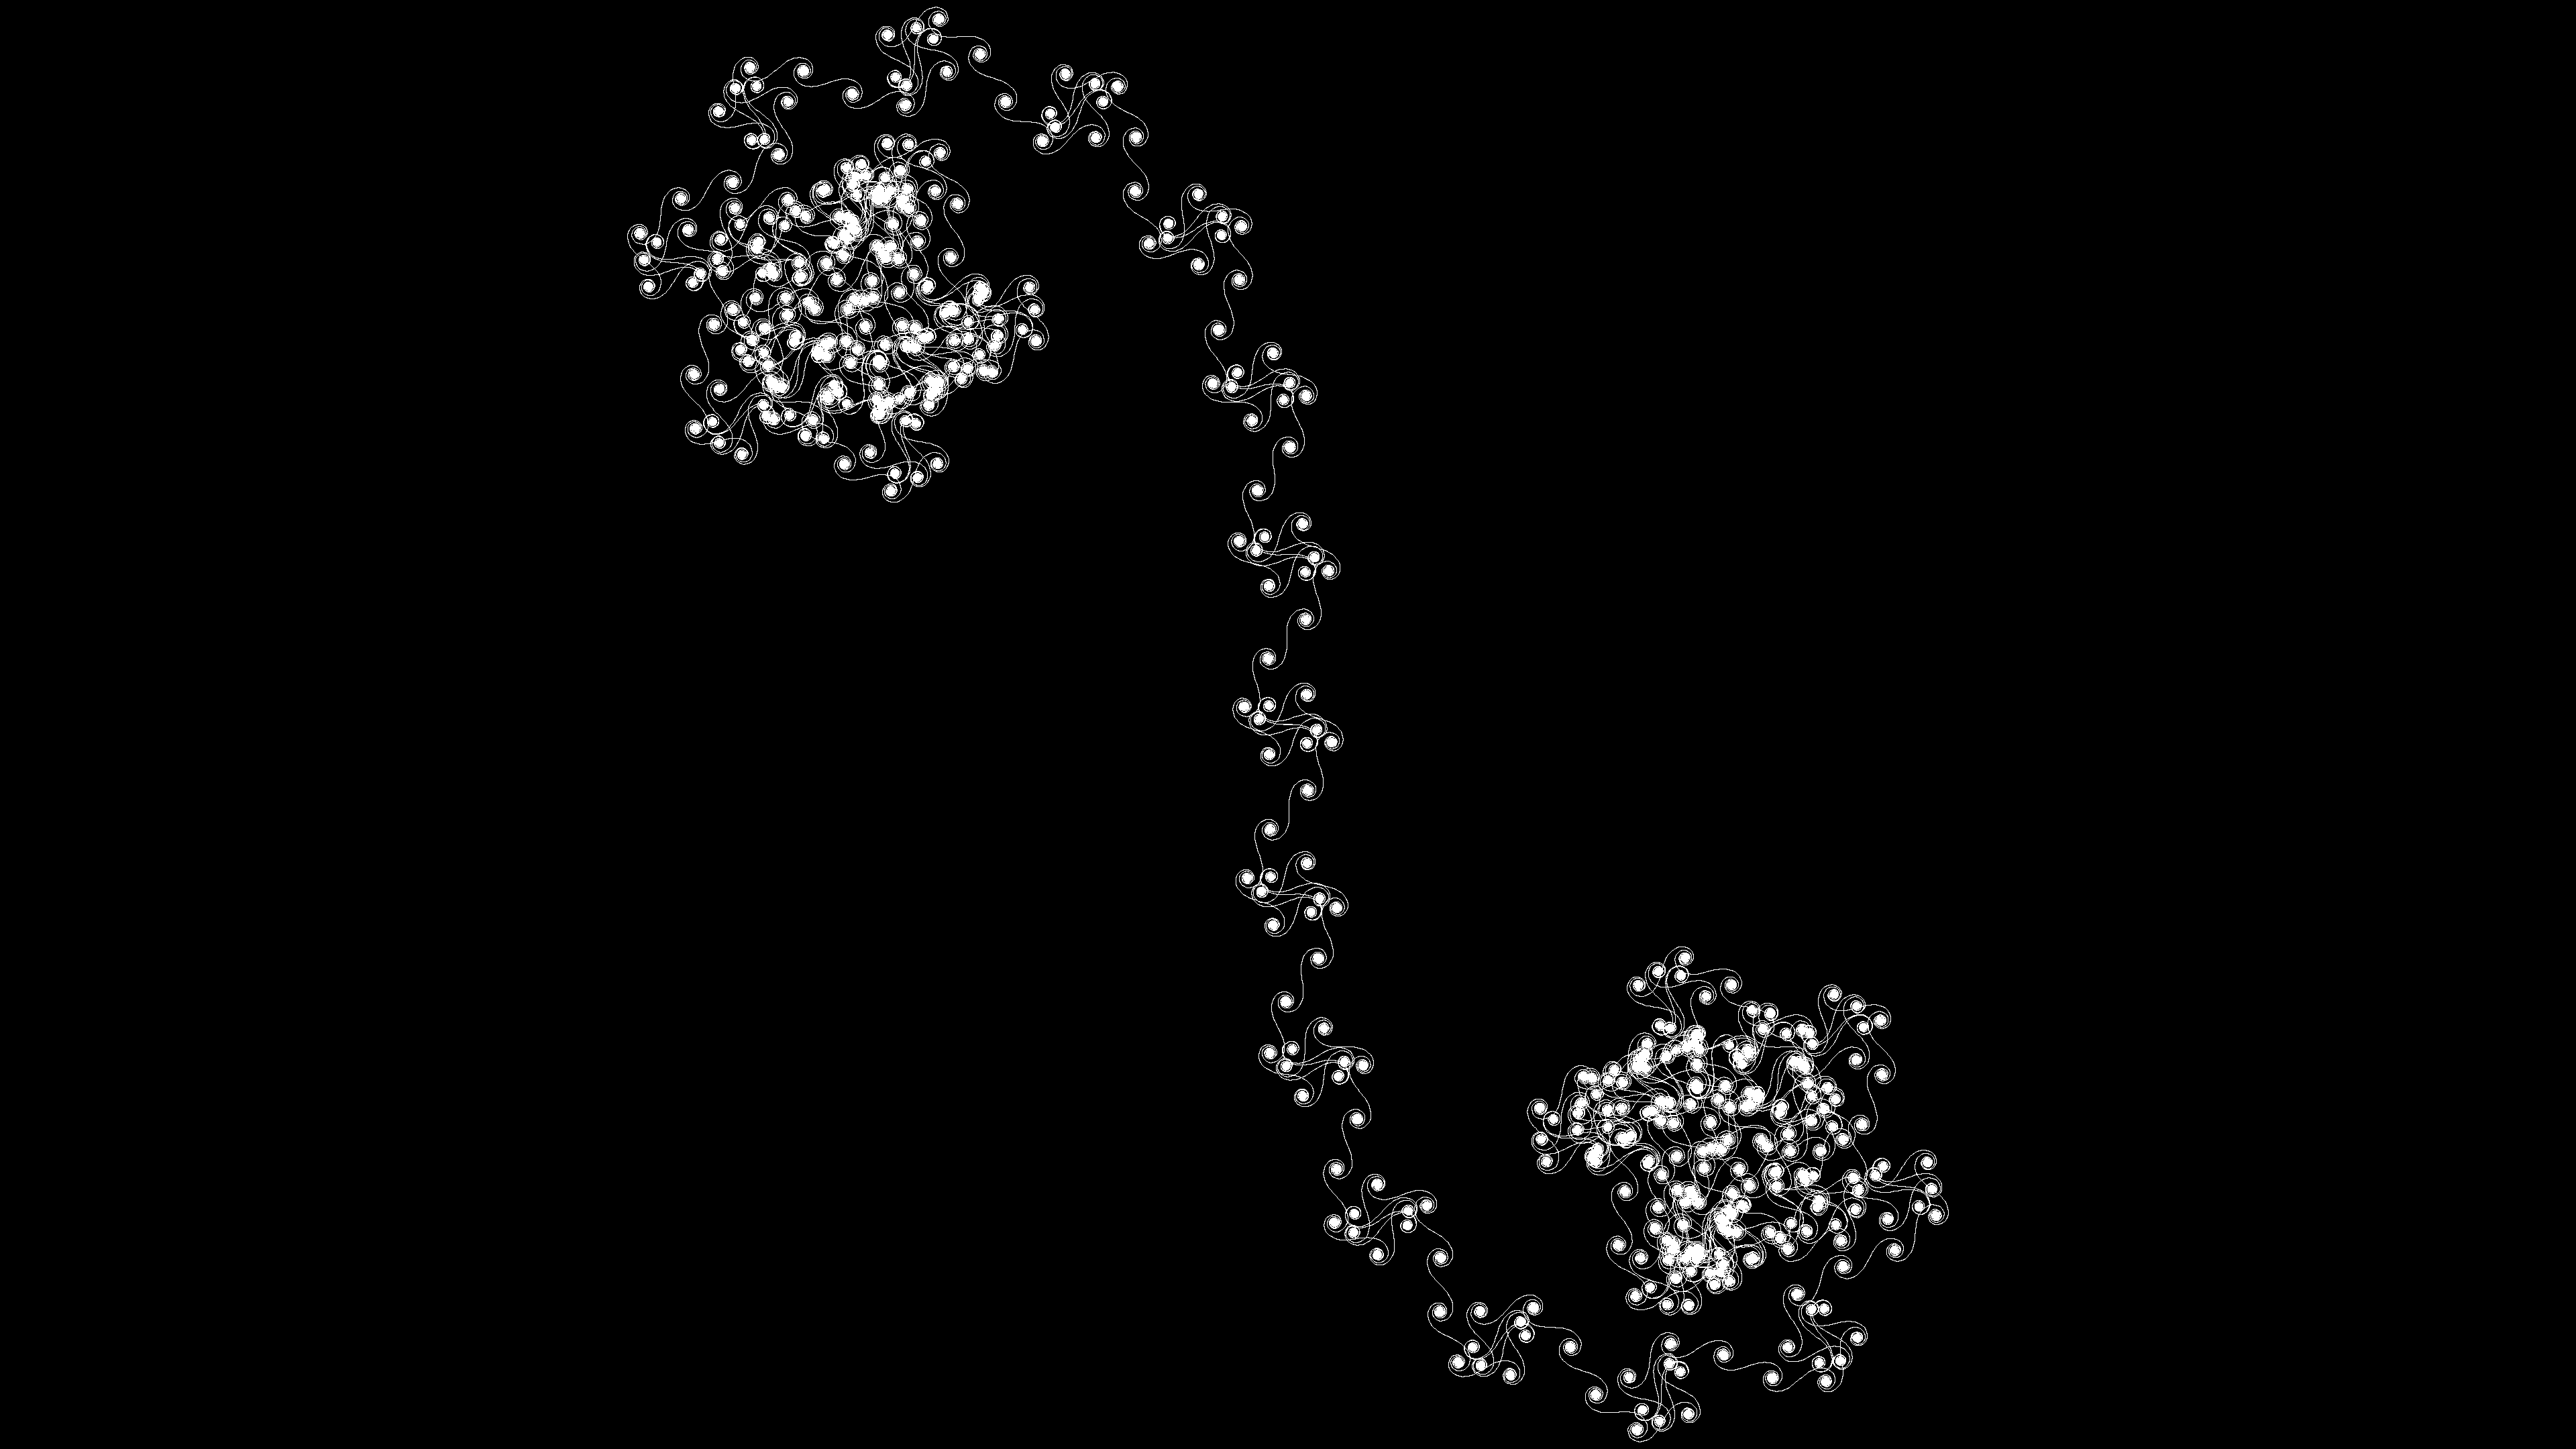
\includegraphics[width=\linewidth]{./stepsplusoneimages/0000000051.png}
    \caption{tf p=499 q=199650 theta=000 89977461.png}
  \end{subfigure}
  \begin{subfigure}[t]{0.48\textwidth}
    \centering
    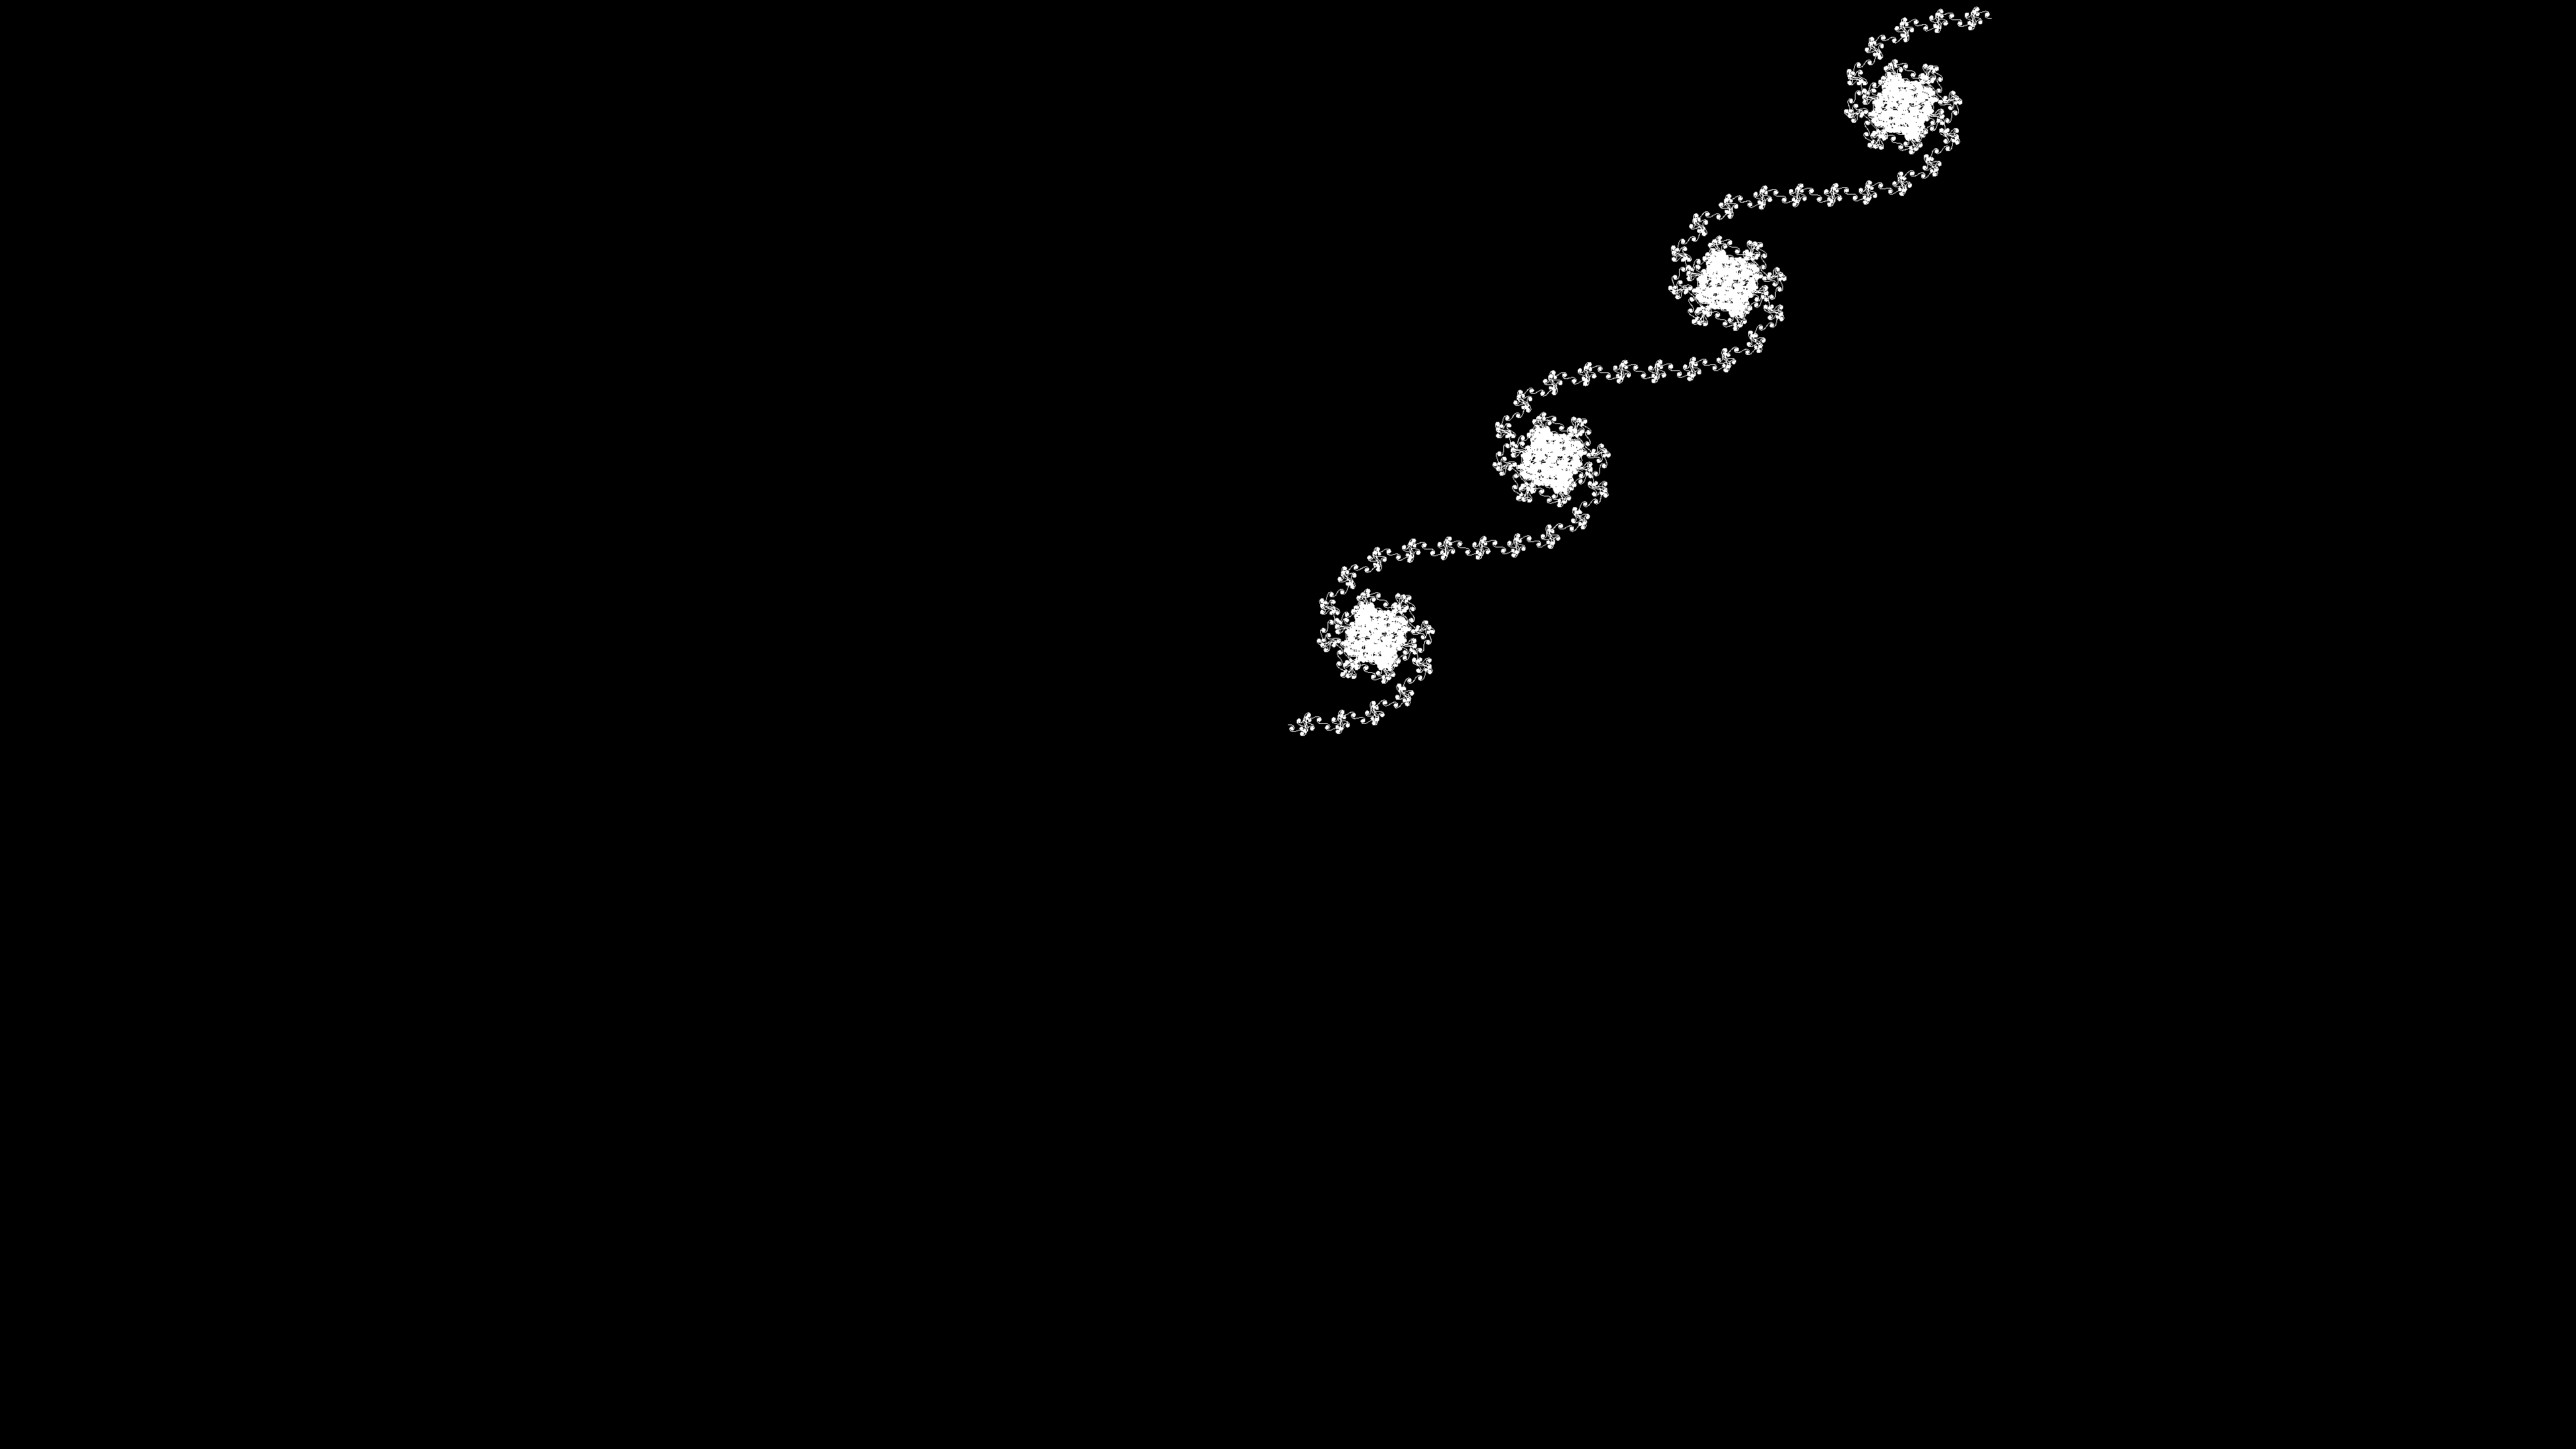
\includegraphics[width=\linewidth]{./stepsplusoneimages/0000000052.png}
    \caption{tf p=499 q=200149 theta=000 89753134.png}
  \end{subfigure}
  \caption{n=050 s=400 s+1=401}
  \label{fig:n=050}
\end{figure}
\begin{figure}[H]
  \centering
  \begin{subfigure}[t]{0.48\textwidth}
    \centering
    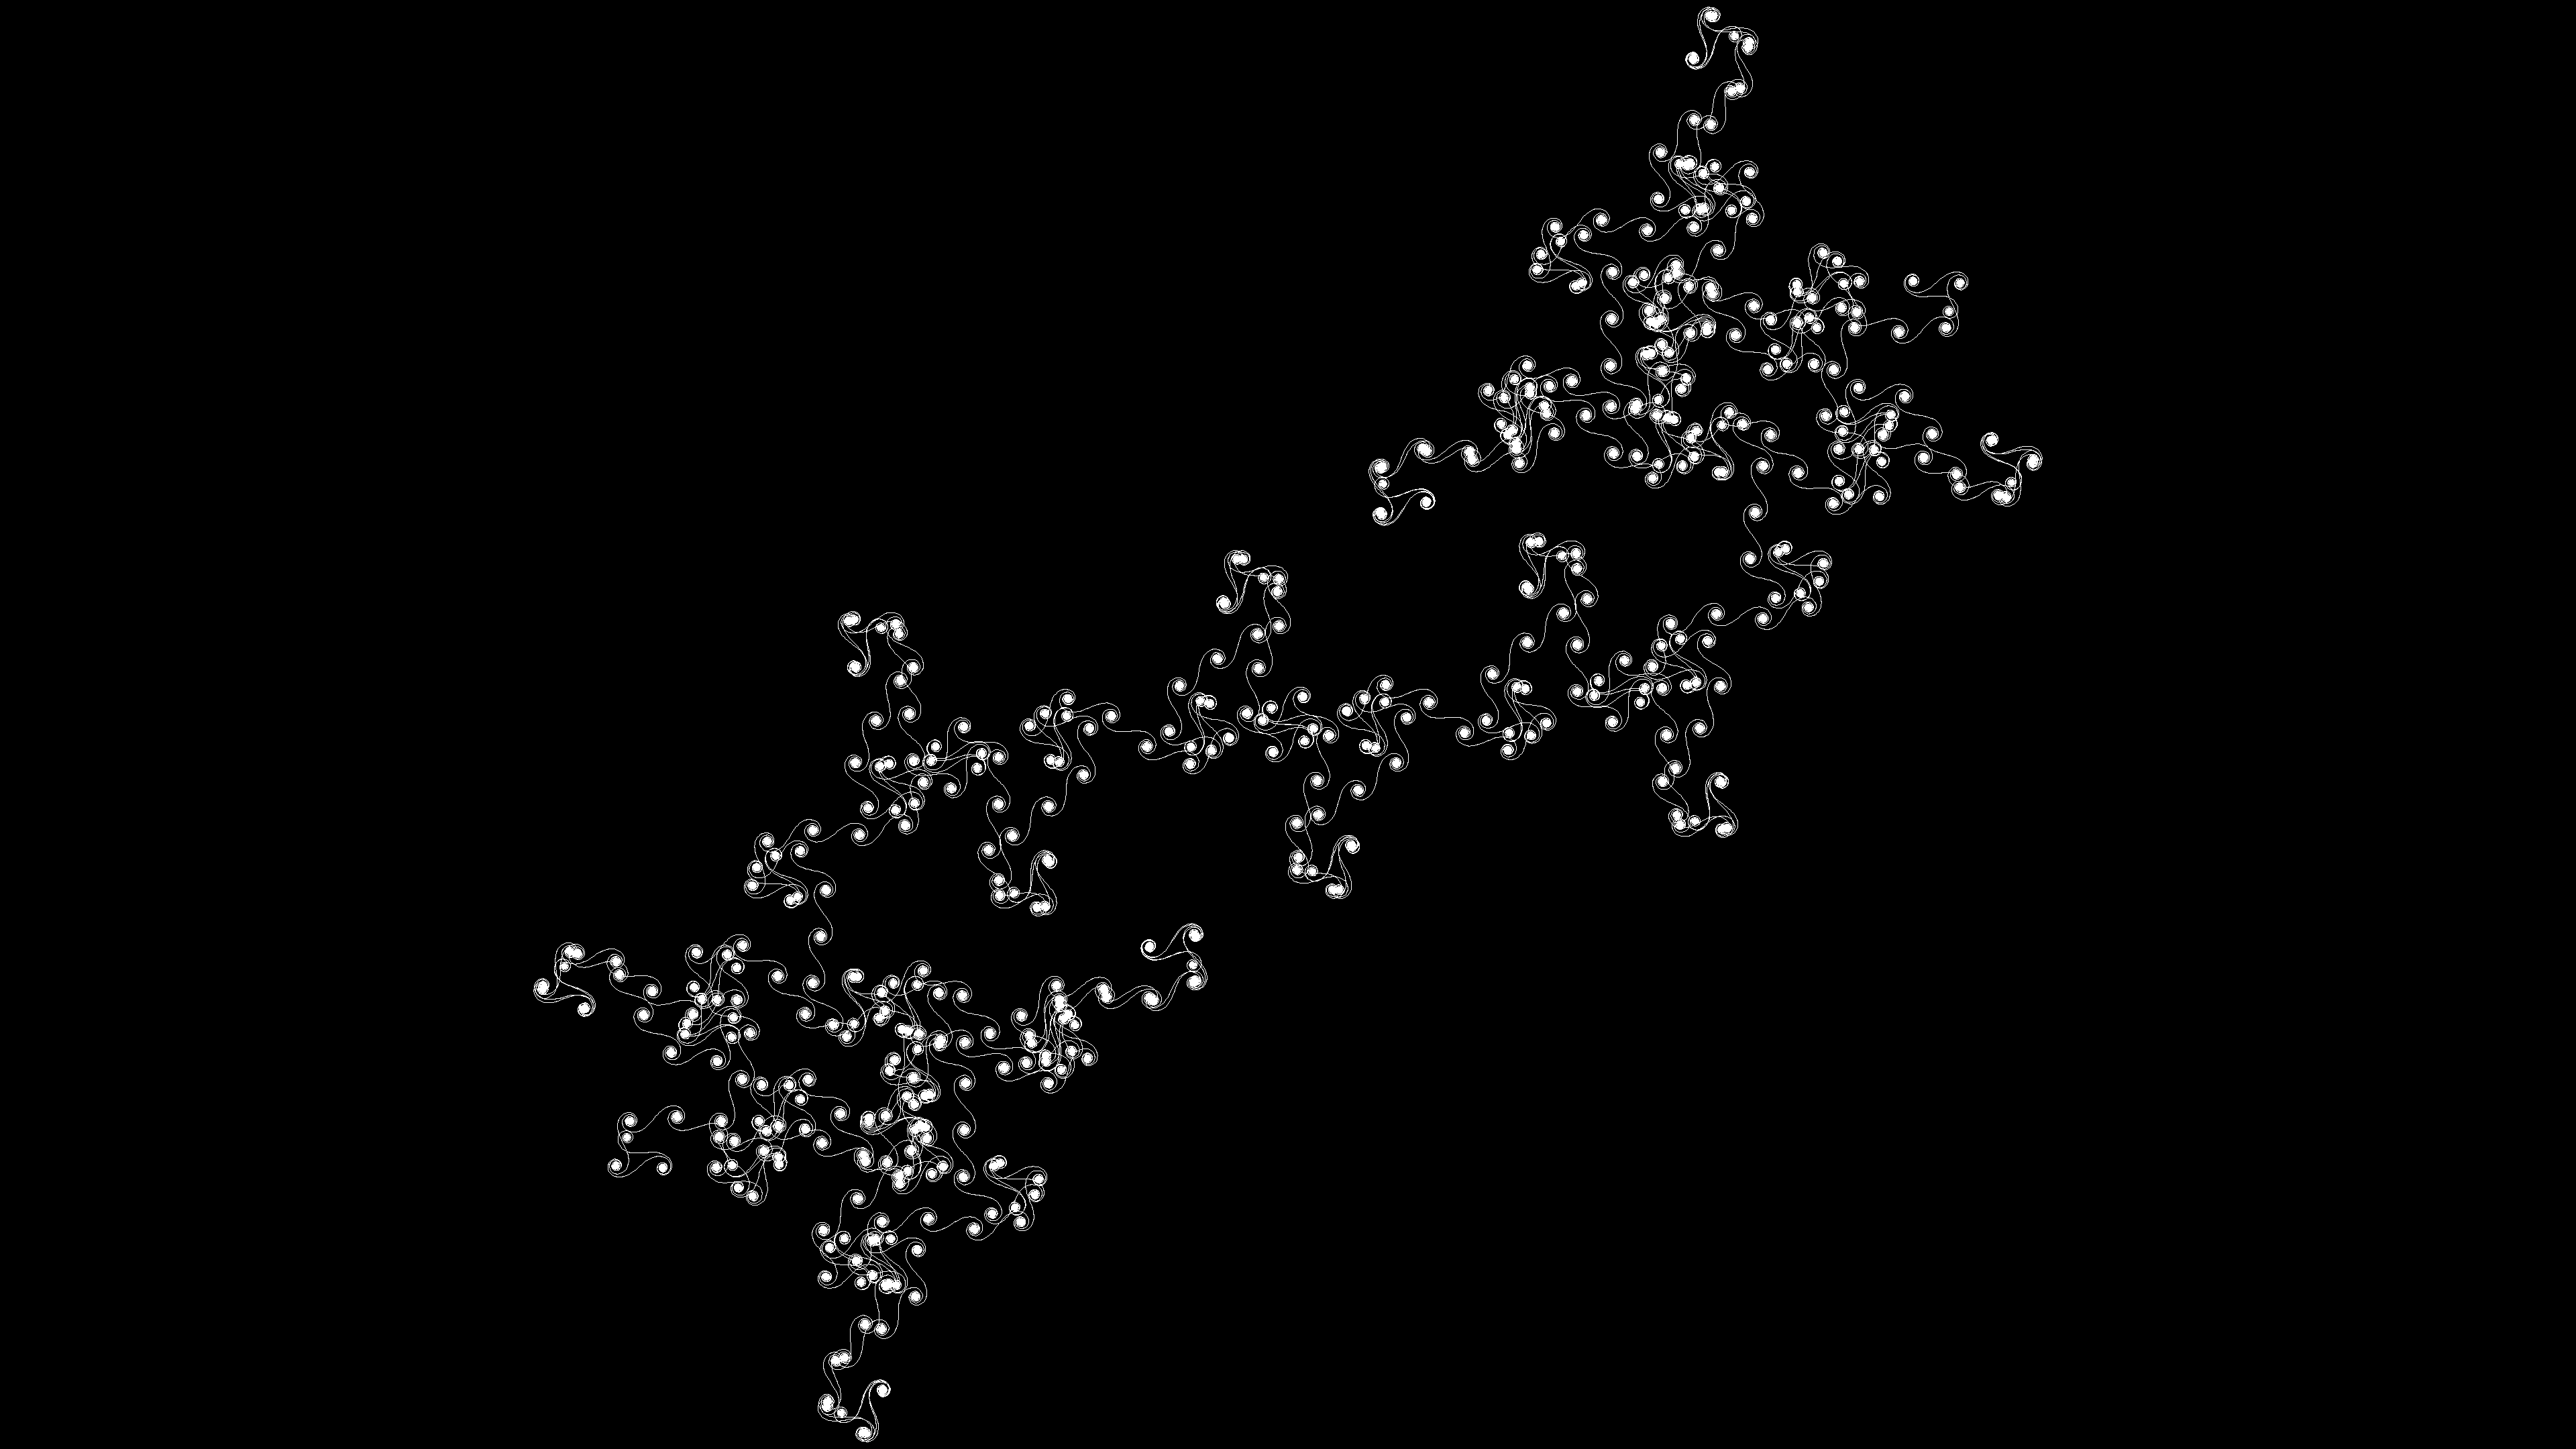
\includegraphics[width=\linewidth]{./stepsplusoneimages/0000000053.png}
    \caption{tf p=499 q=199652 theta=000 89976559.png}
  \end{subfigure}
  \begin{subfigure}[t]{0.48\textwidth}
    \centering
    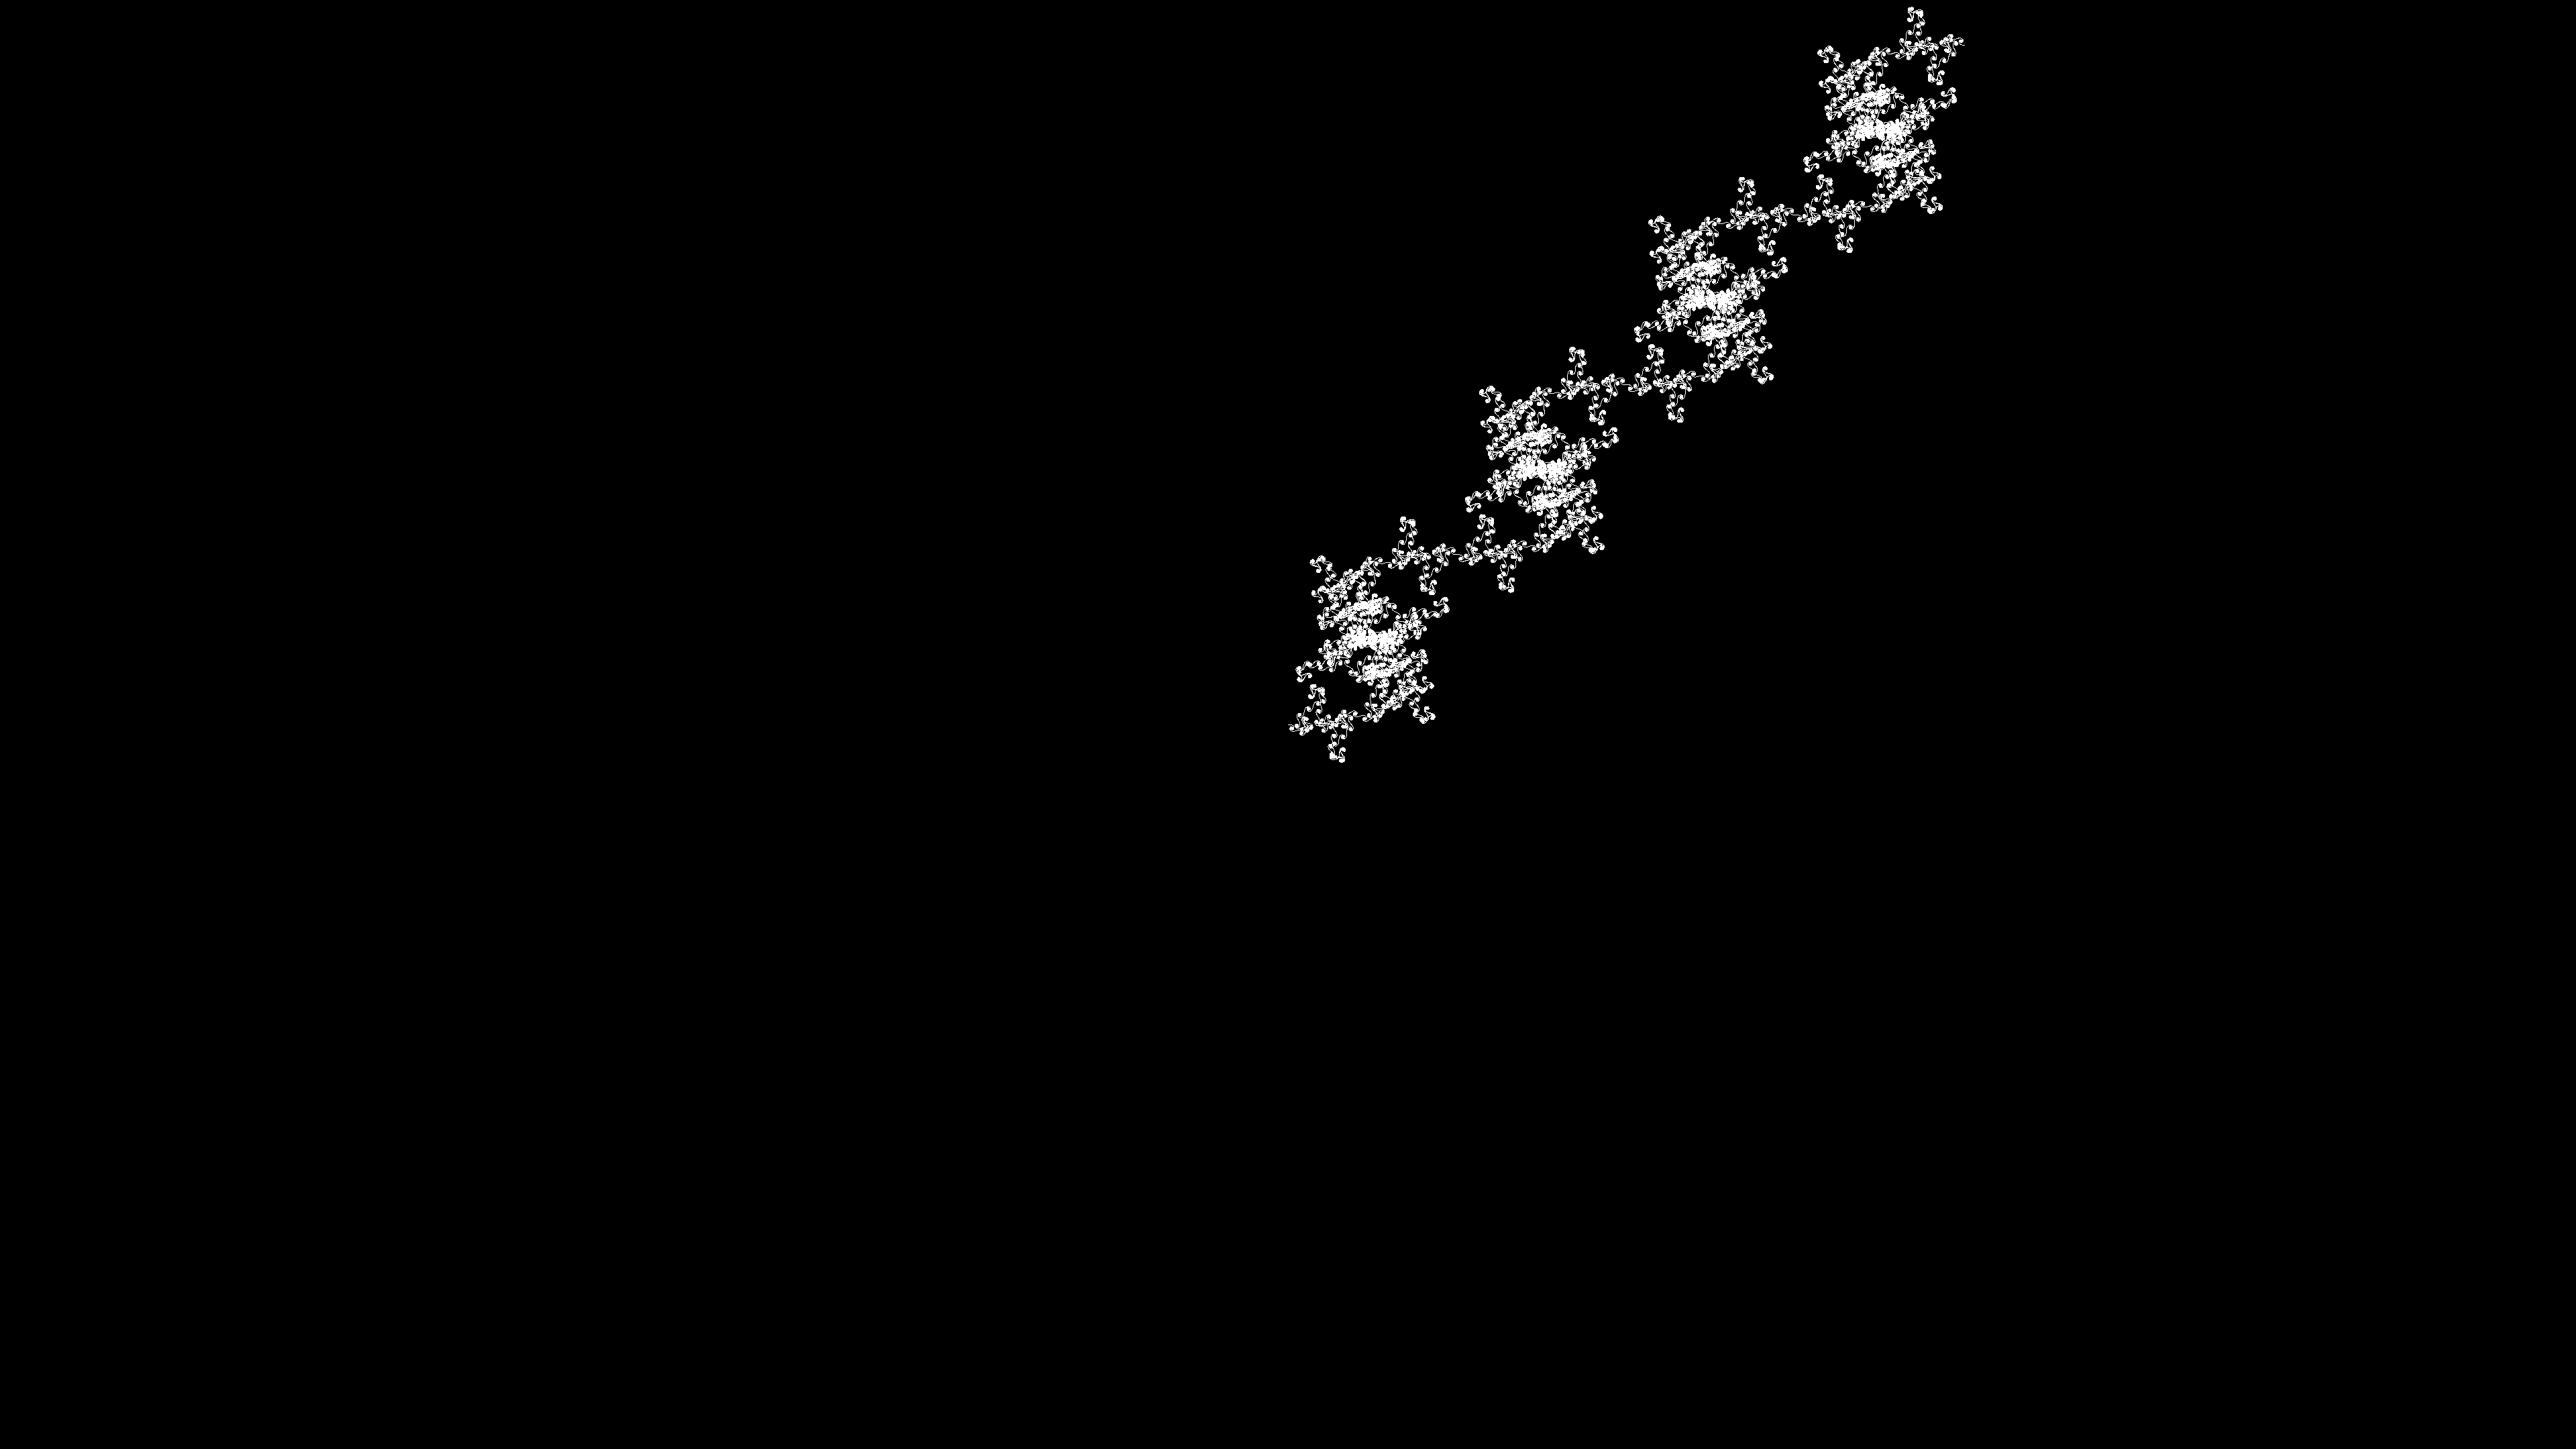
\includegraphics[width=\linewidth]{./stepsplusoneimages/0000000054.png}
    \caption{tf p=499 q=200151 theta=000 89752237.png}
  \end{subfigure}
  \caption{n=052 s=400 s+1=401}
  \label{fig:n=052}
\end{figure}
\begin{figure}[H]
  \centering
  \begin{subfigure}[t]{0.48\textwidth}
    \centering
    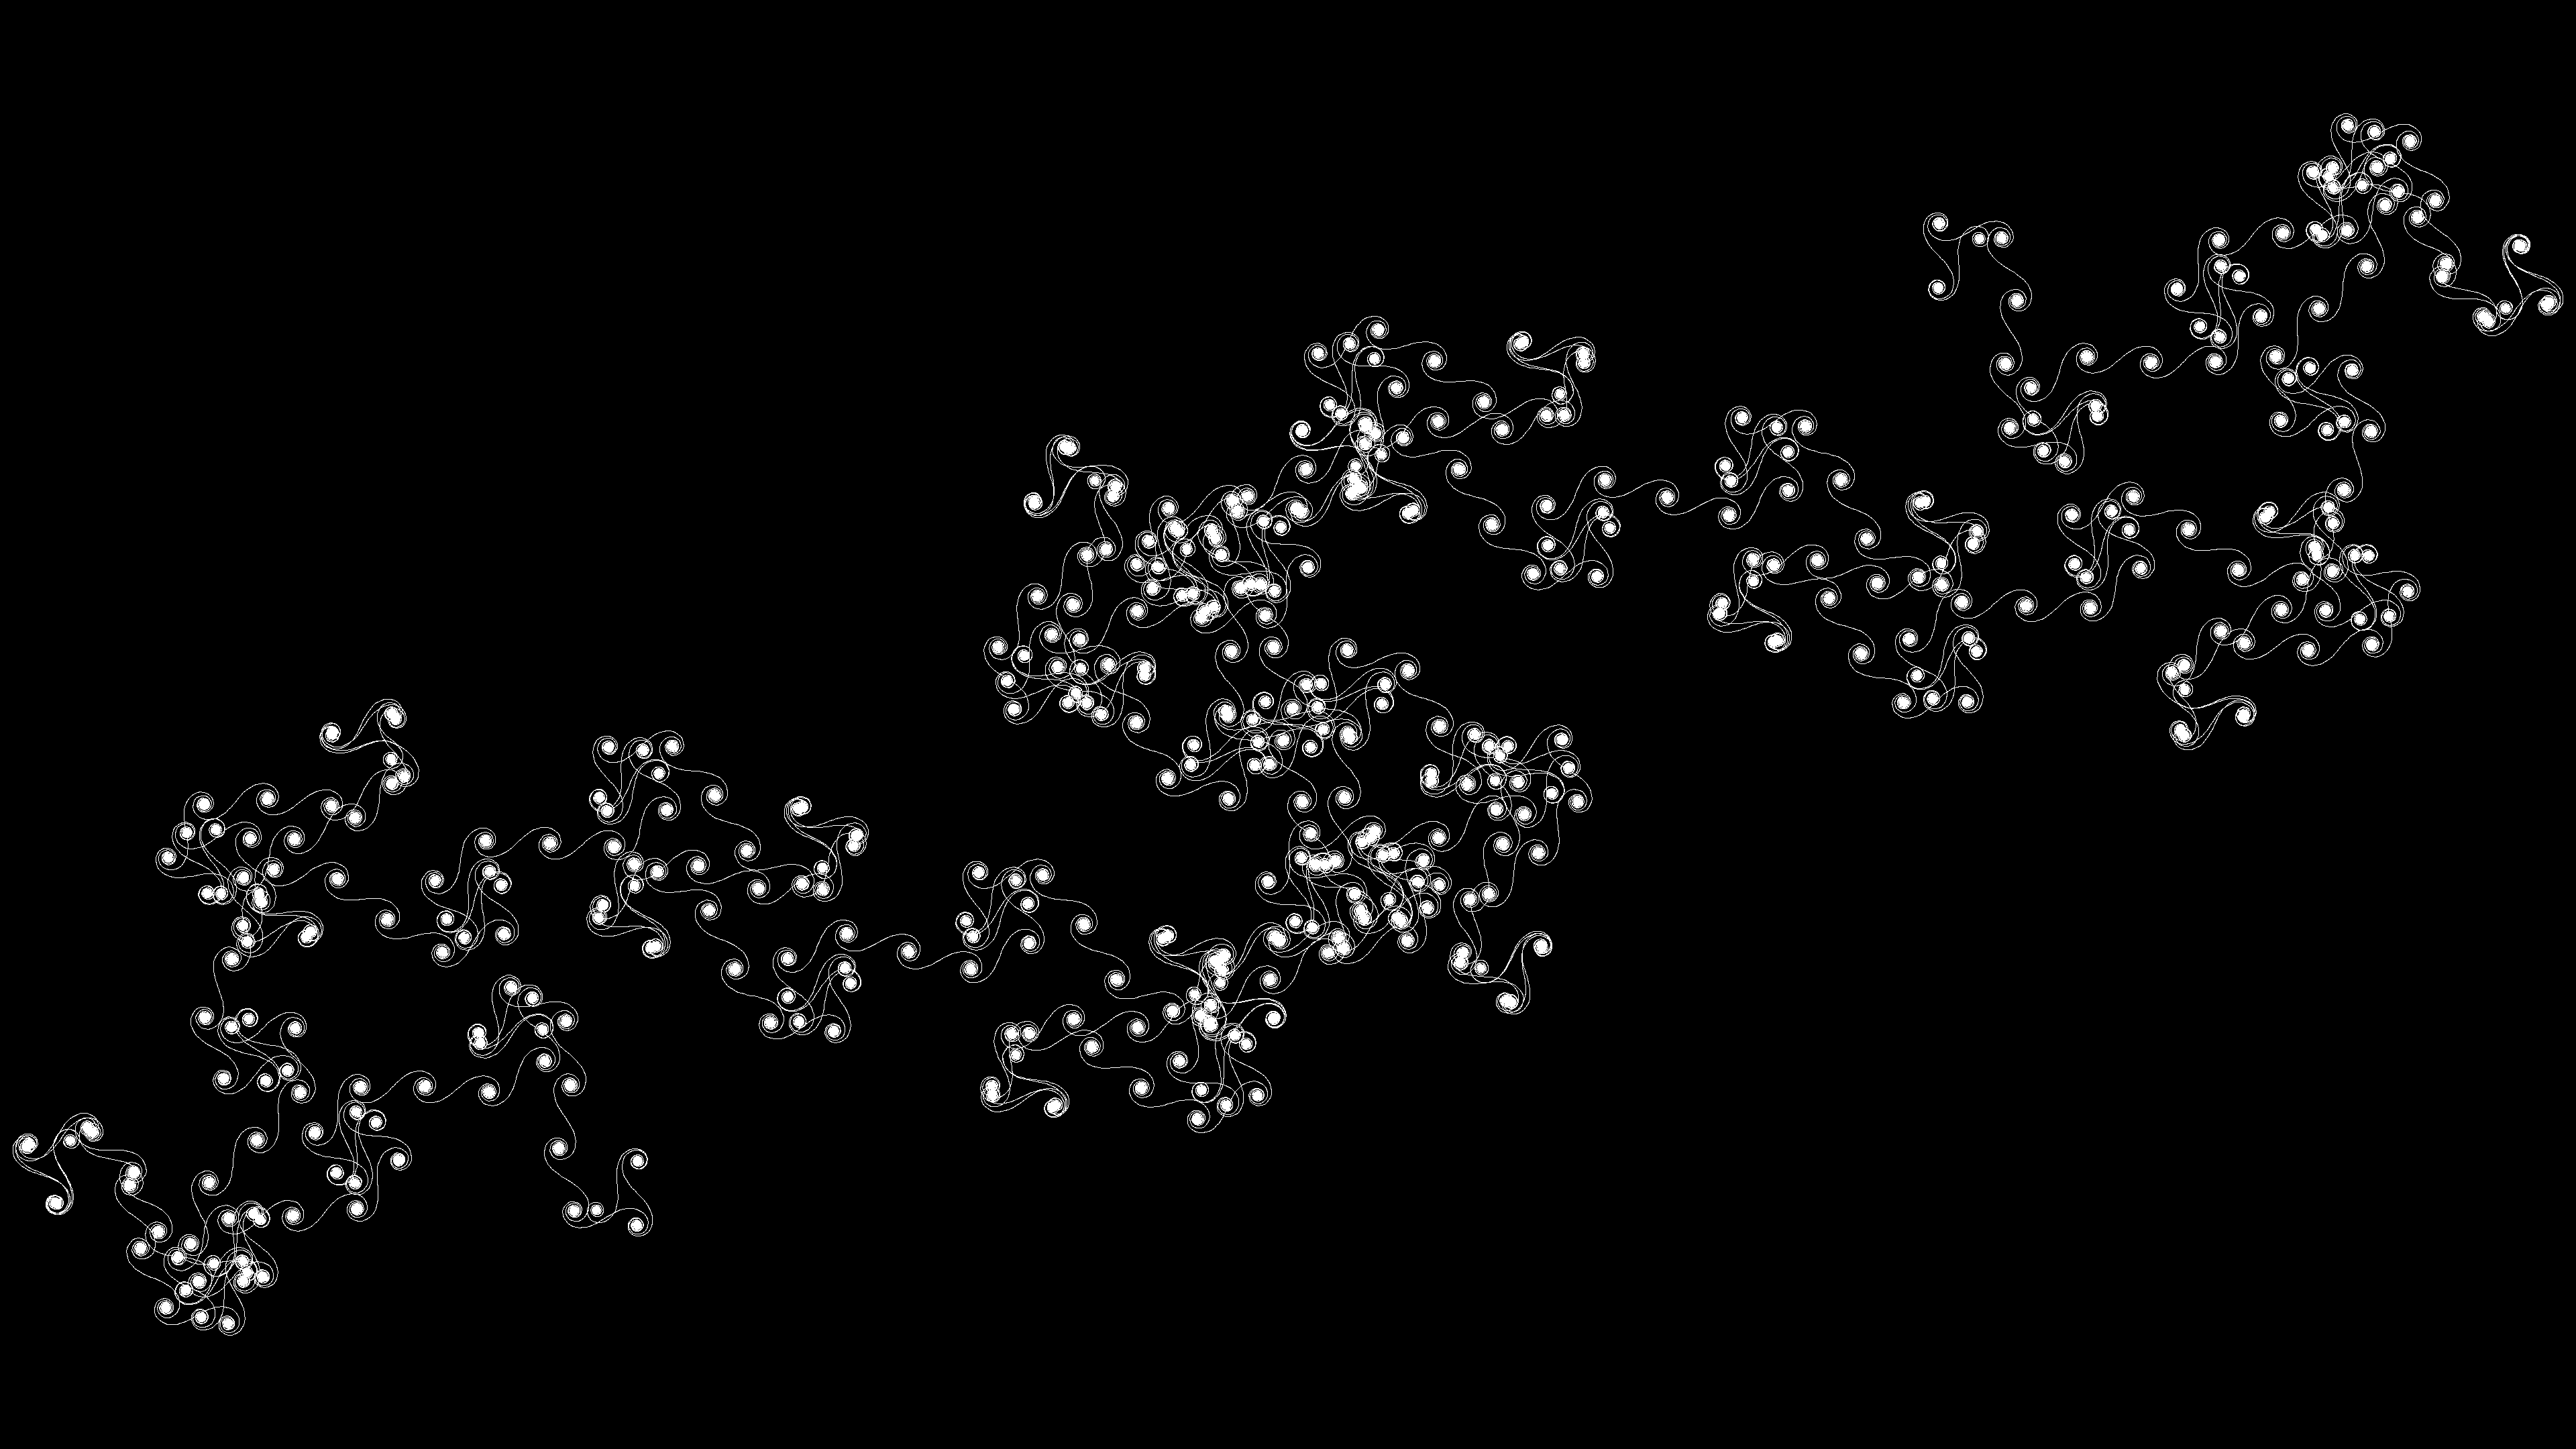
\includegraphics[width=\linewidth]{./stepsplusoneimages/0000000055.png}
    \caption{tf p=499 q=199654 theta=000 89975658.png}
  \end{subfigure}
  \begin{subfigure}[t]{0.48\textwidth}
    \centering
    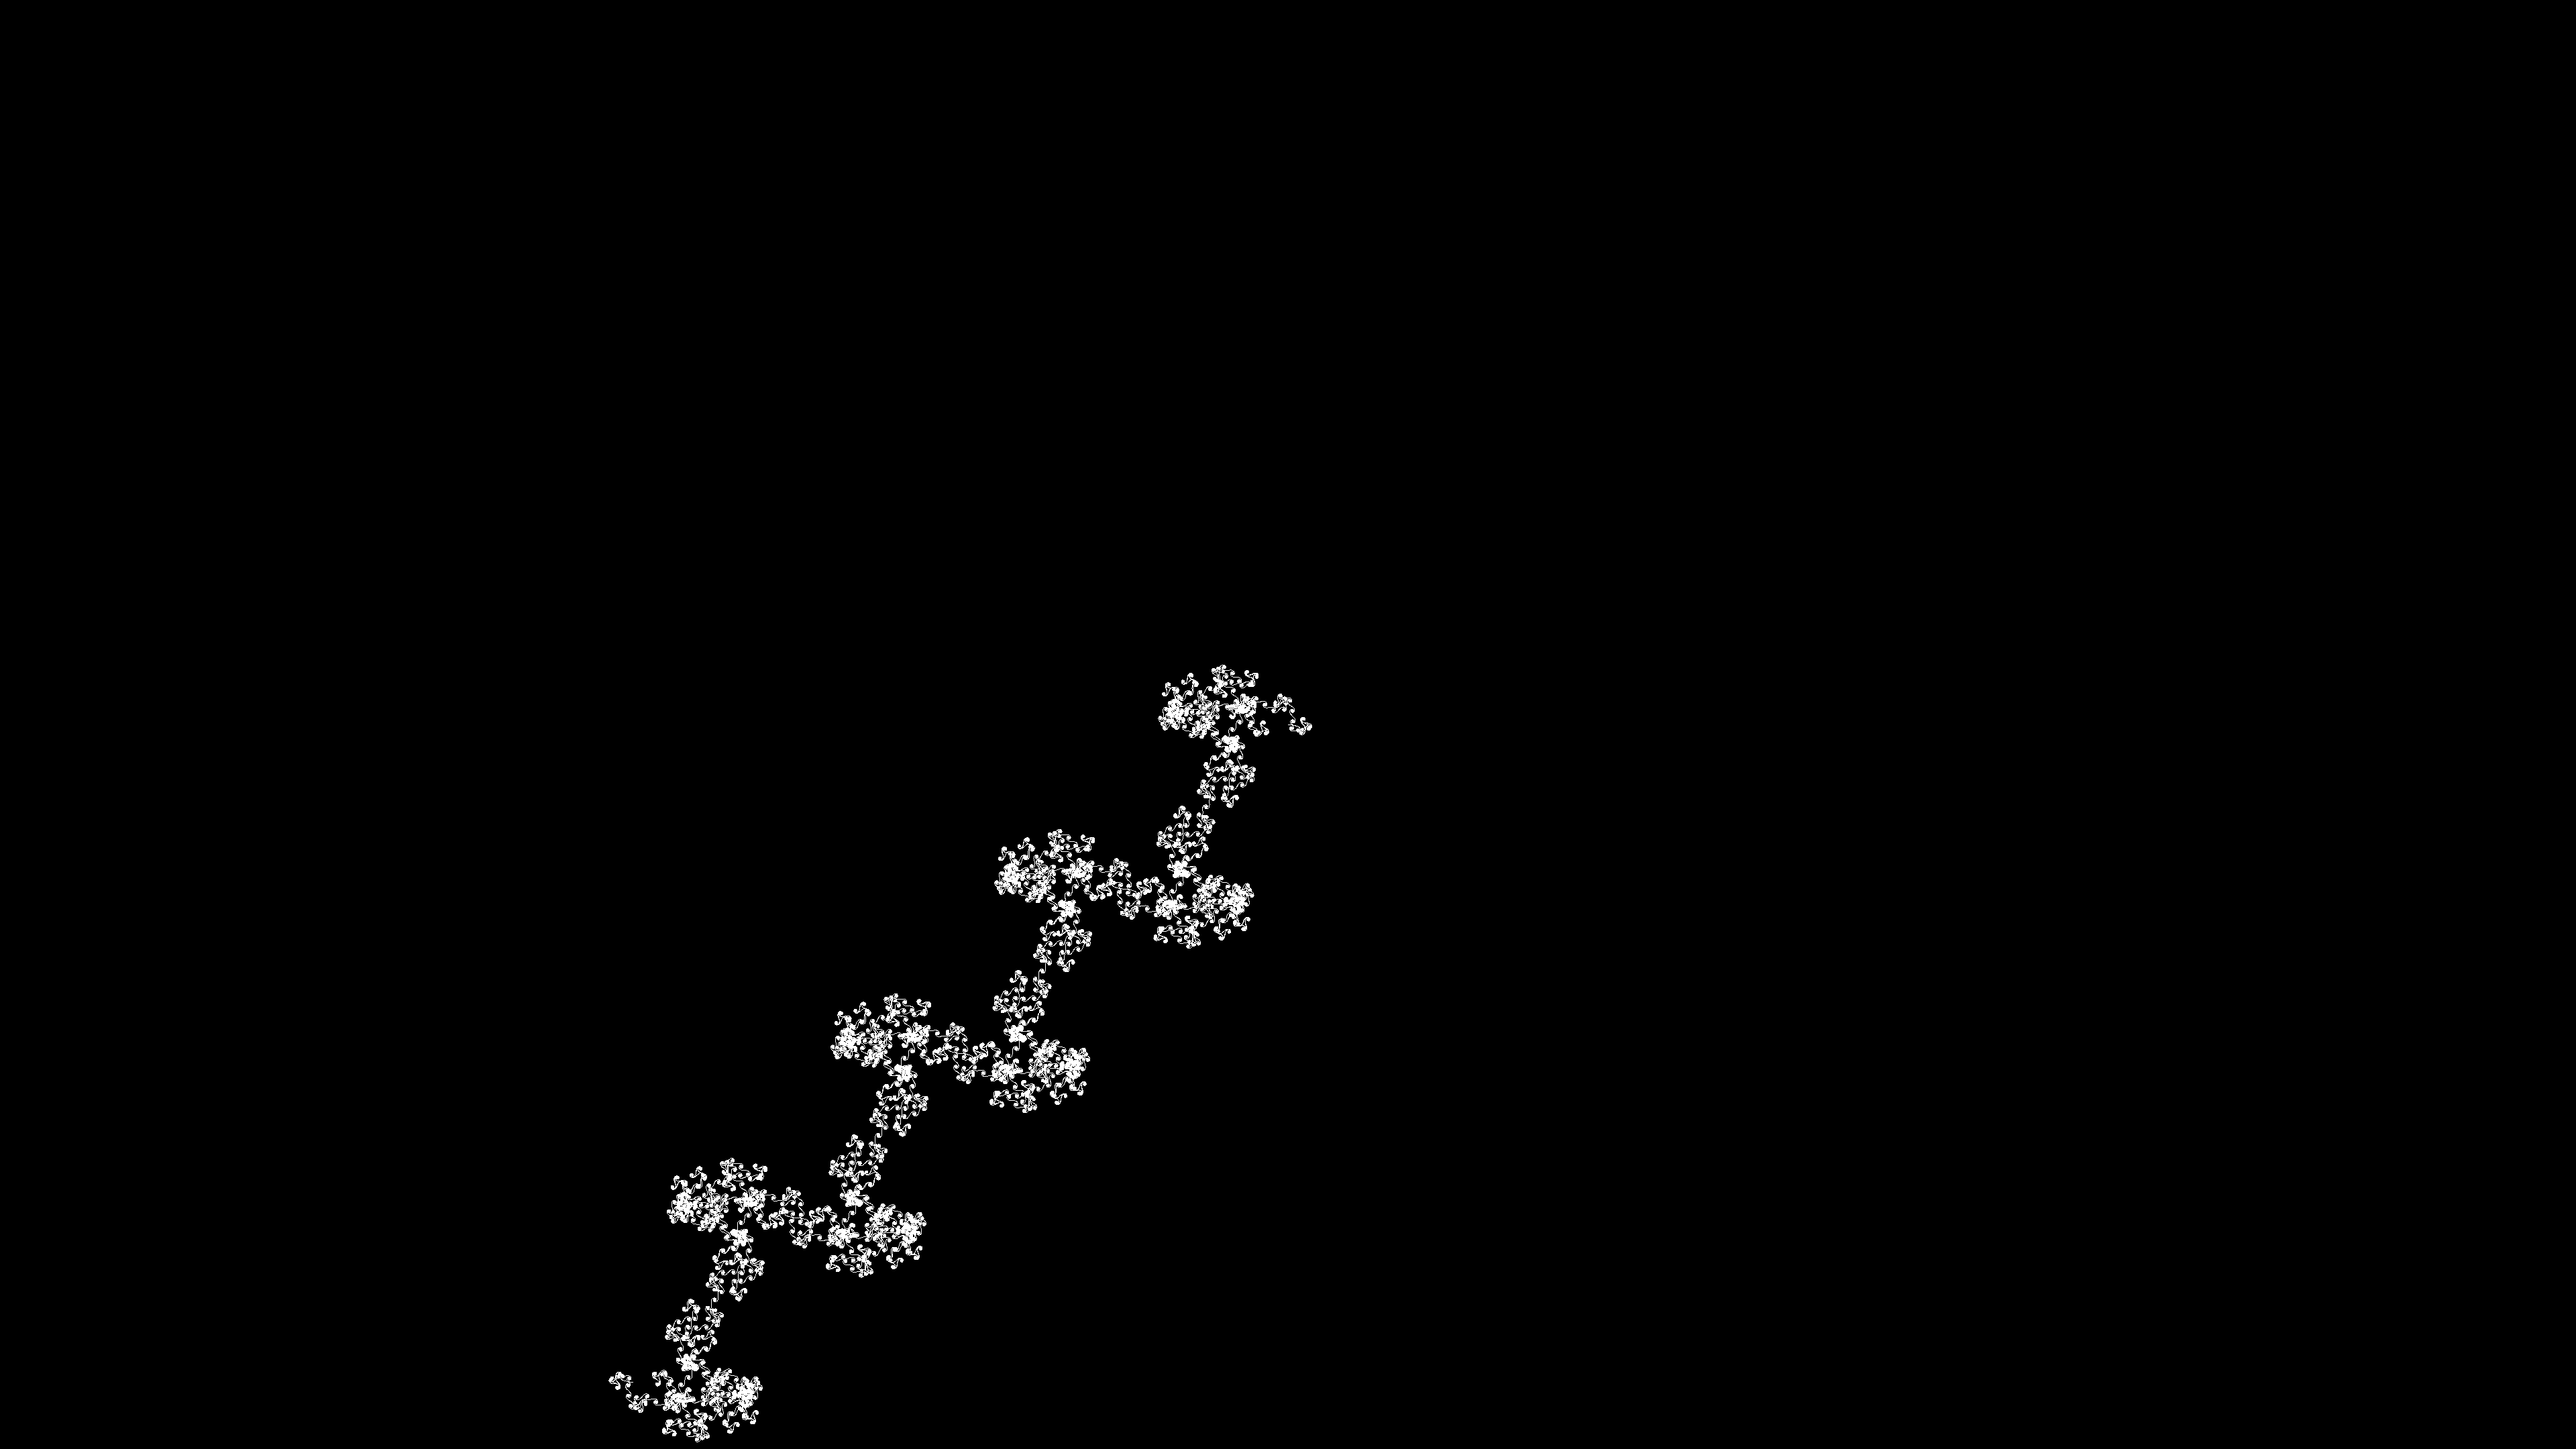
\includegraphics[width=\linewidth]{./stepsplusoneimages/0000000056.png}
    \caption{tf p=499 q=200153 theta=000 89751340.png}
  \end{subfigure}
  \caption{n=054 s=400 s+1=401}
  \label{fig:n=054}
\end{figure}
\begin{figure}[H]
  \centering
  \begin{subfigure}[t]{0.48\textwidth}
    \centering
    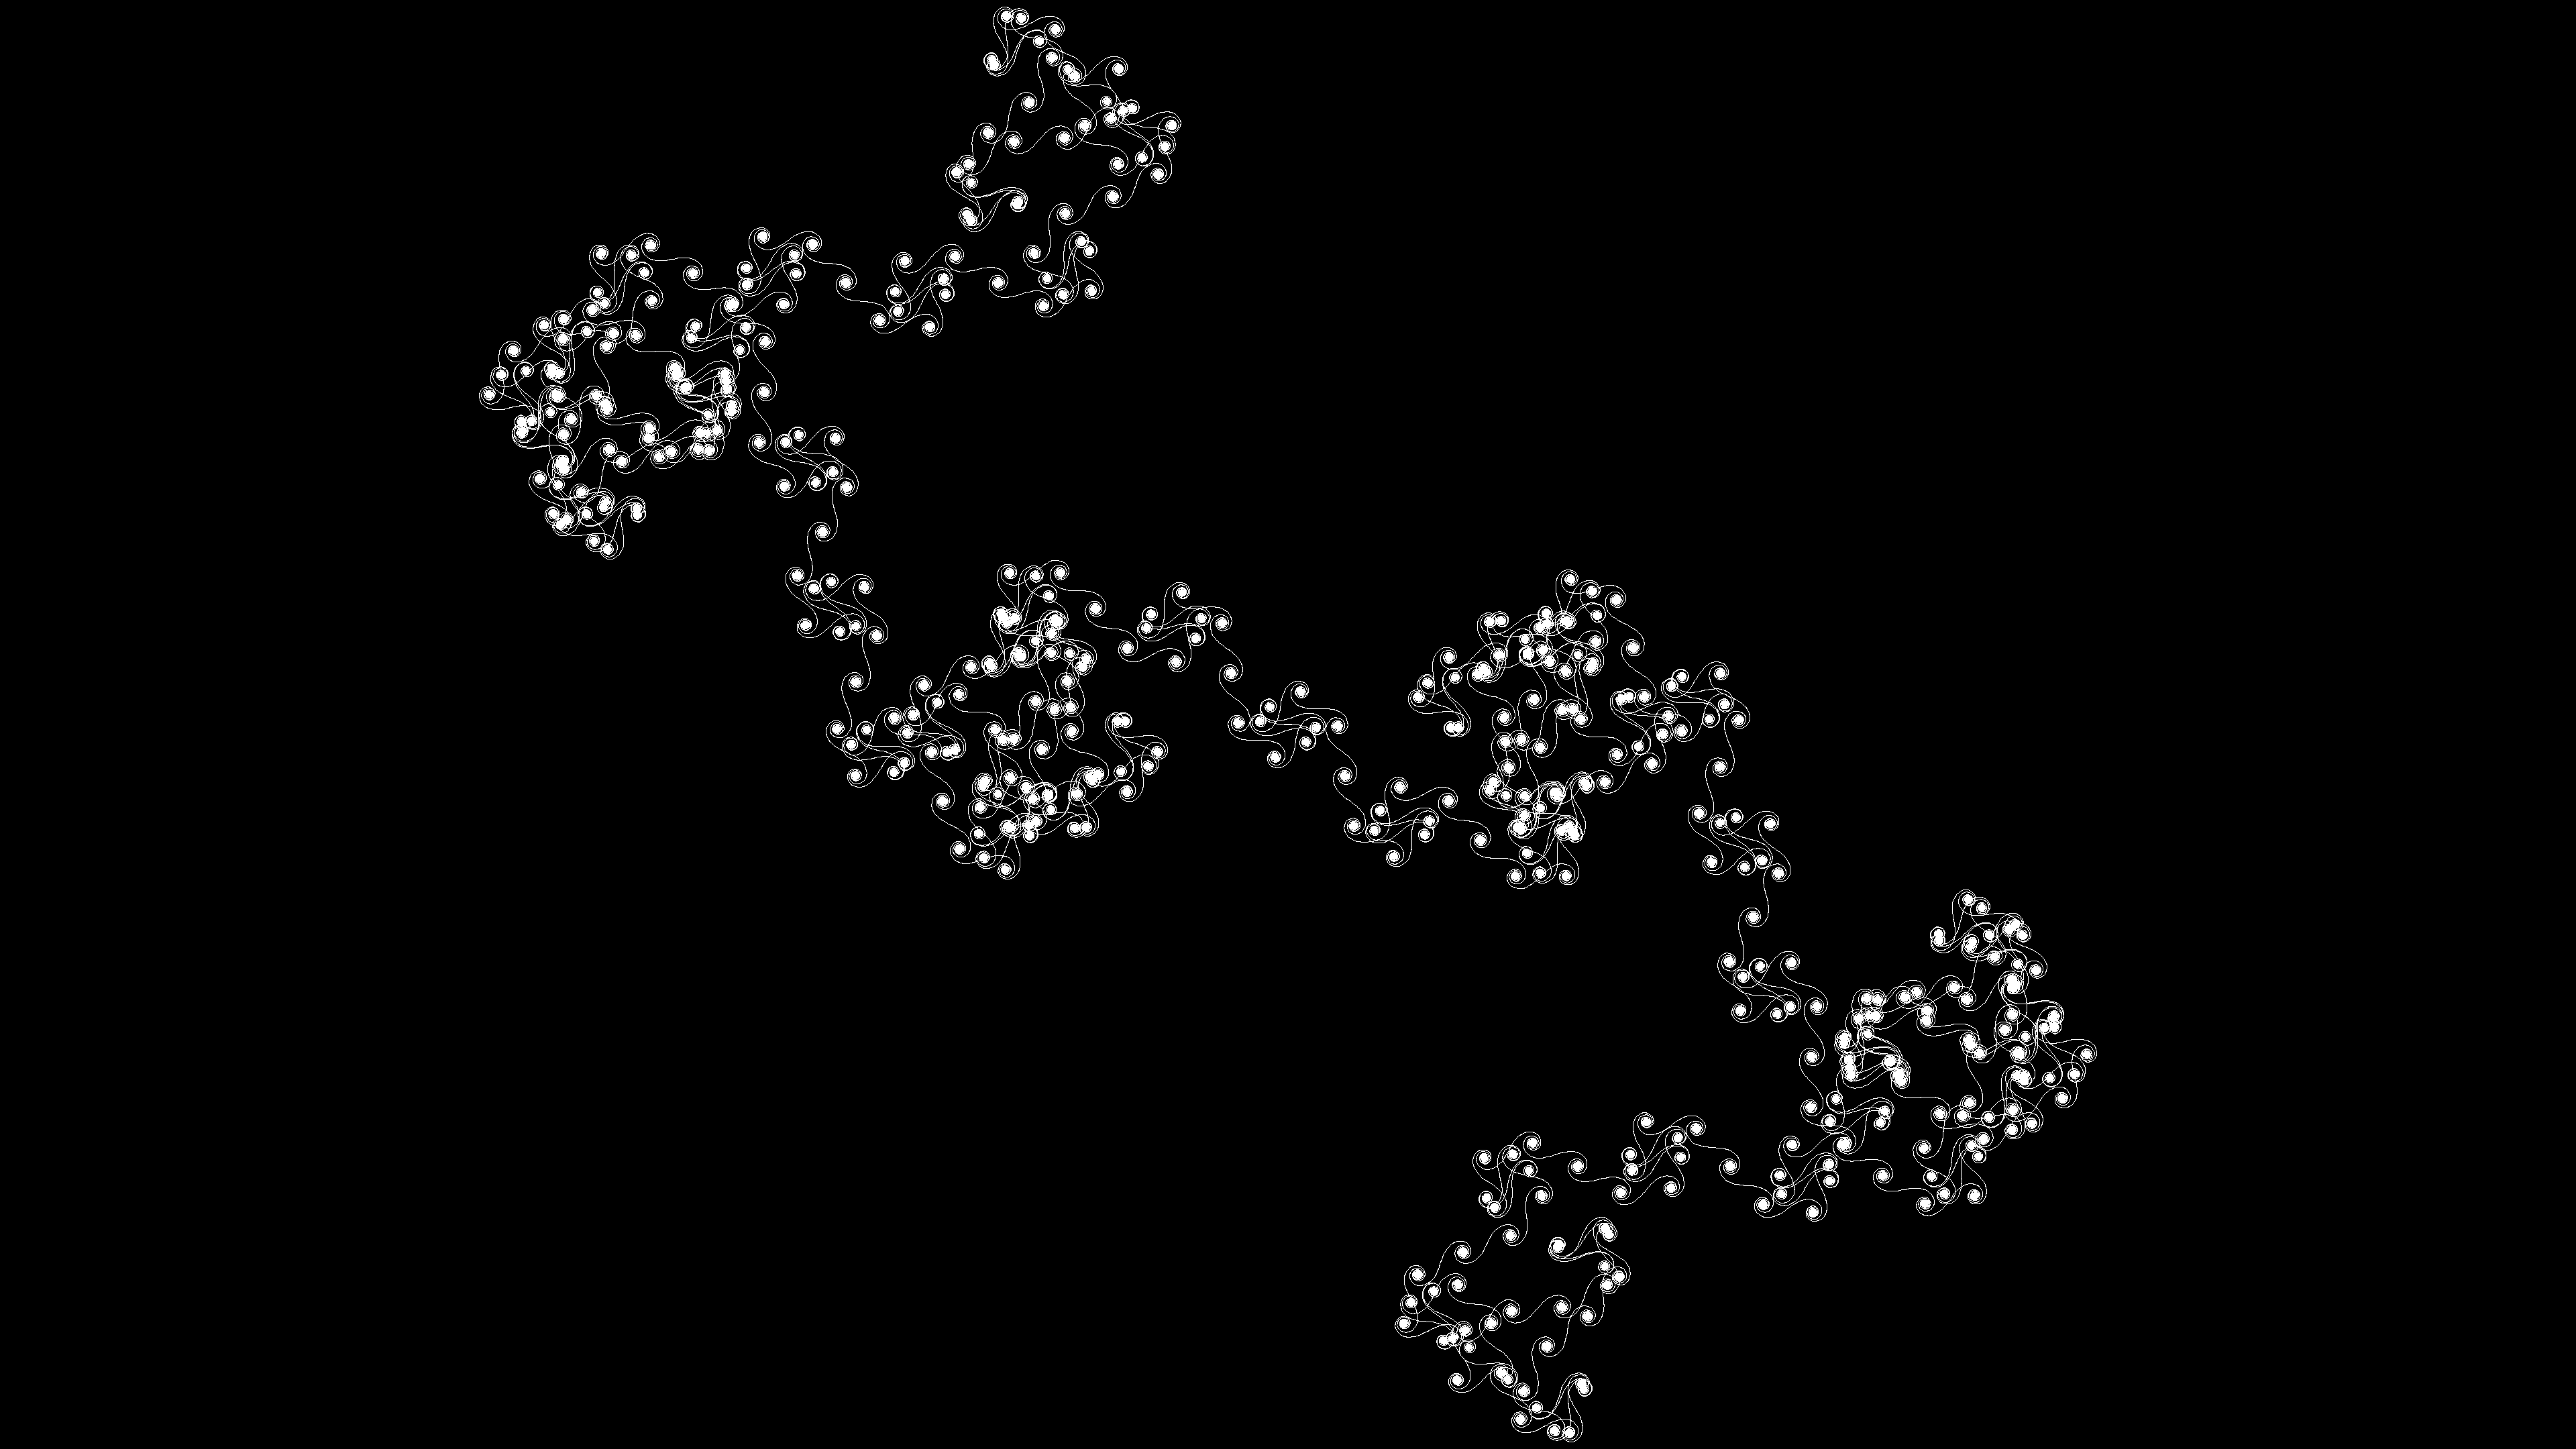
\includegraphics[width=\linewidth]{./stepsplusoneimages/0000000057.png}
    \caption{tf p=499 q=199656 theta=000 89974757.png}
  \end{subfigure}
  \begin{subfigure}[t]{0.48\textwidth}
    \centering
    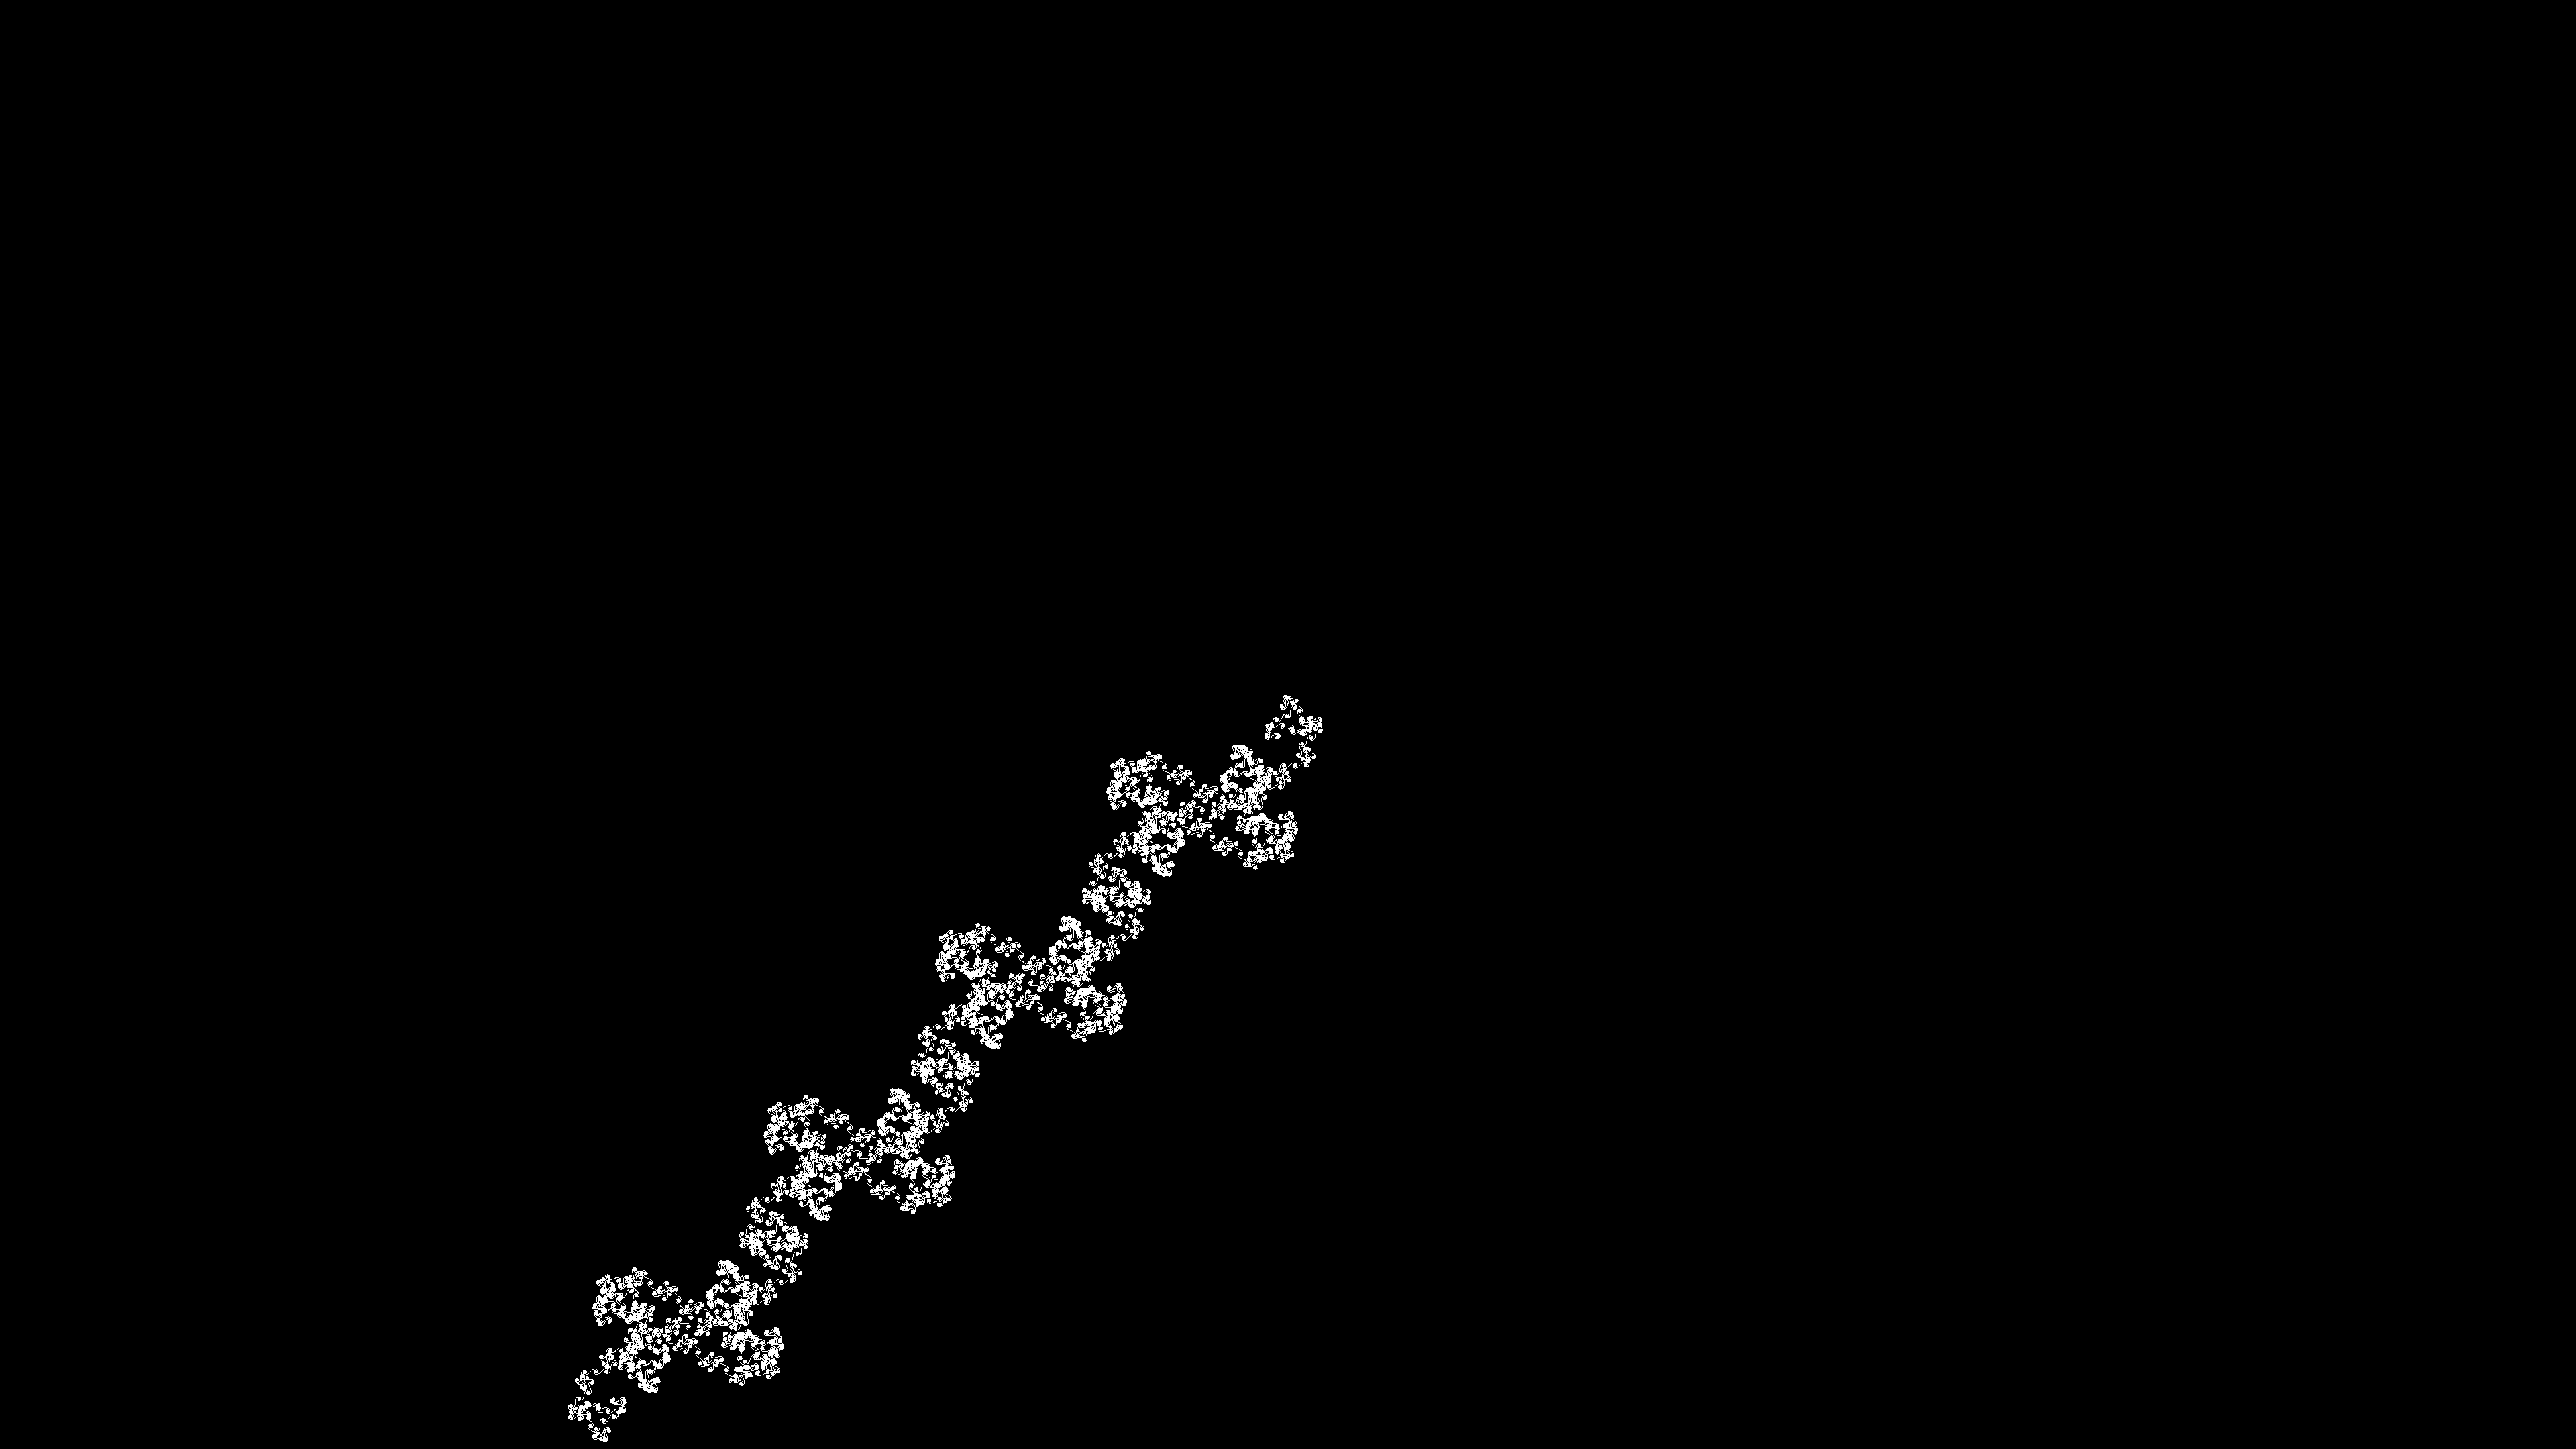
\includegraphics[width=\linewidth]{./stepsplusoneimages/0000000058.png}
    \caption{tf p=499 q=200155 theta=000 89750443.png}
  \end{subfigure}
  \caption{n=056 s=400 s+1=401}
  \label{fig:n=056}
\end{figure}
\begin{figure}[H]
  \centering
  \begin{subfigure}[t]{0.48\textwidth}
    \centering
    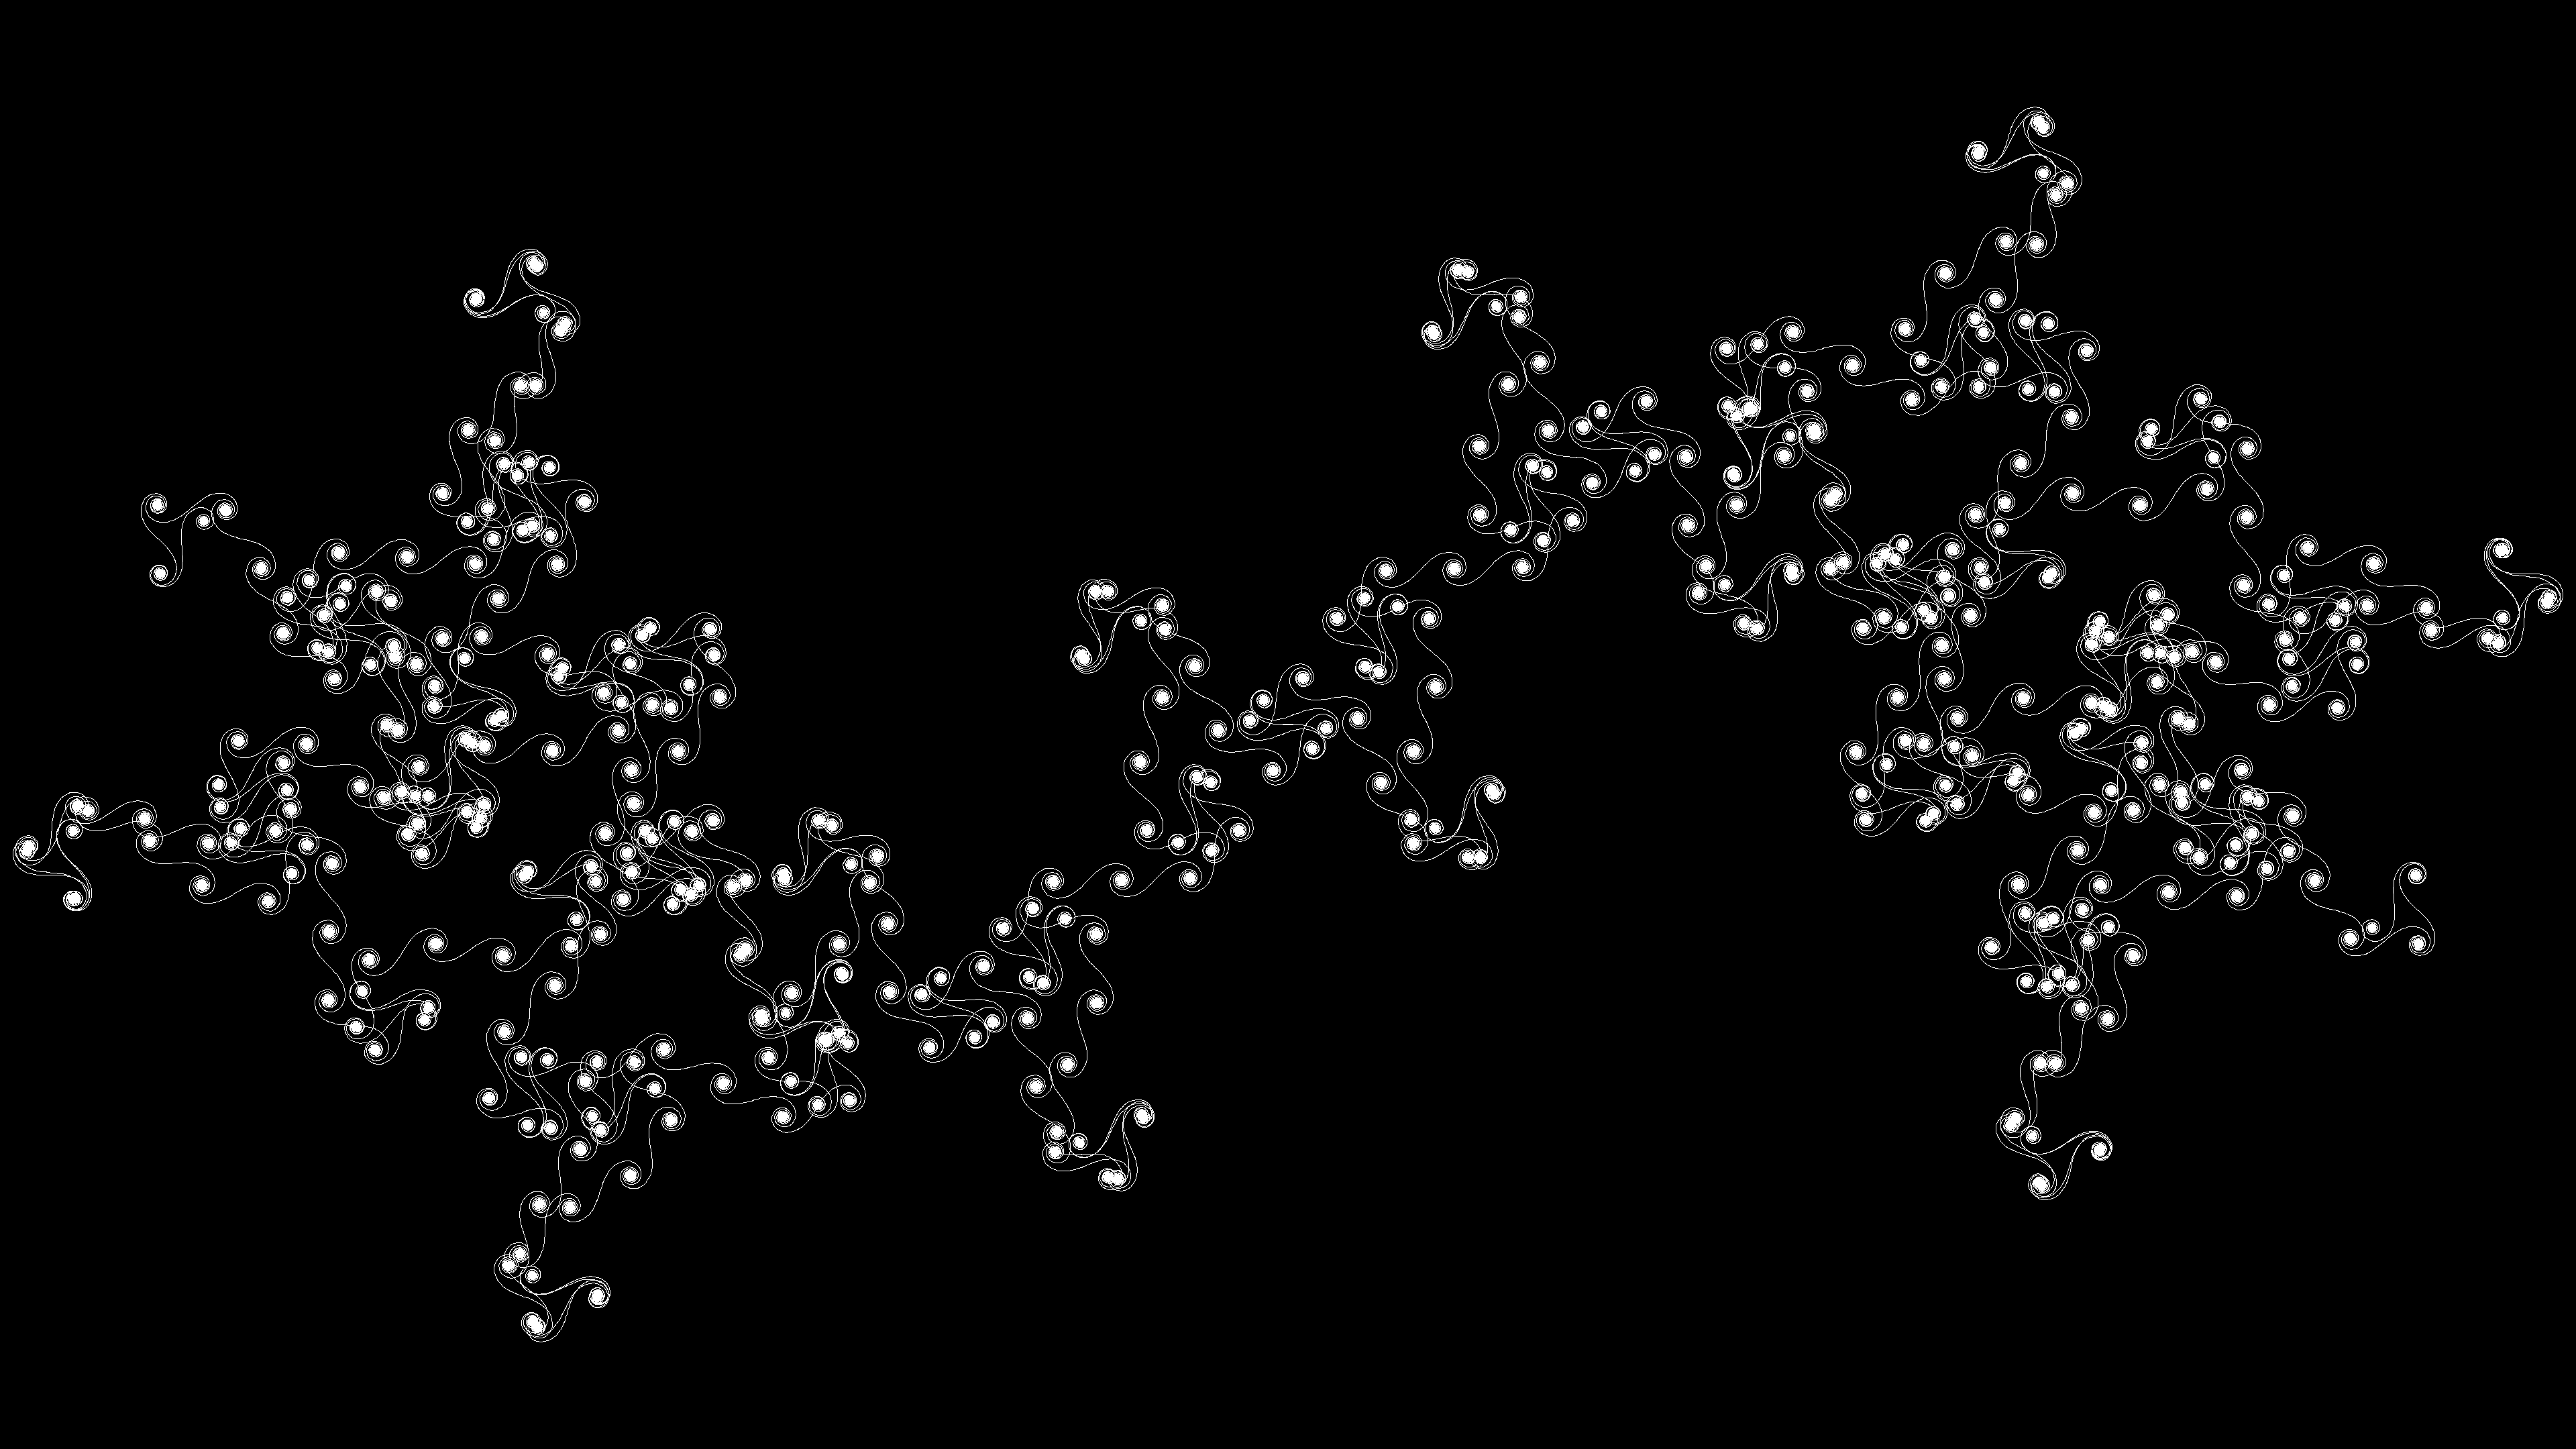
\includegraphics[width=\linewidth]{./stepsplusoneimages/0000000059.png}
    \caption{tf p=499 q=199658 theta=000 89973855.png}
  \end{subfigure}
  \begin{subfigure}[t]{0.48\textwidth}
    \centering
    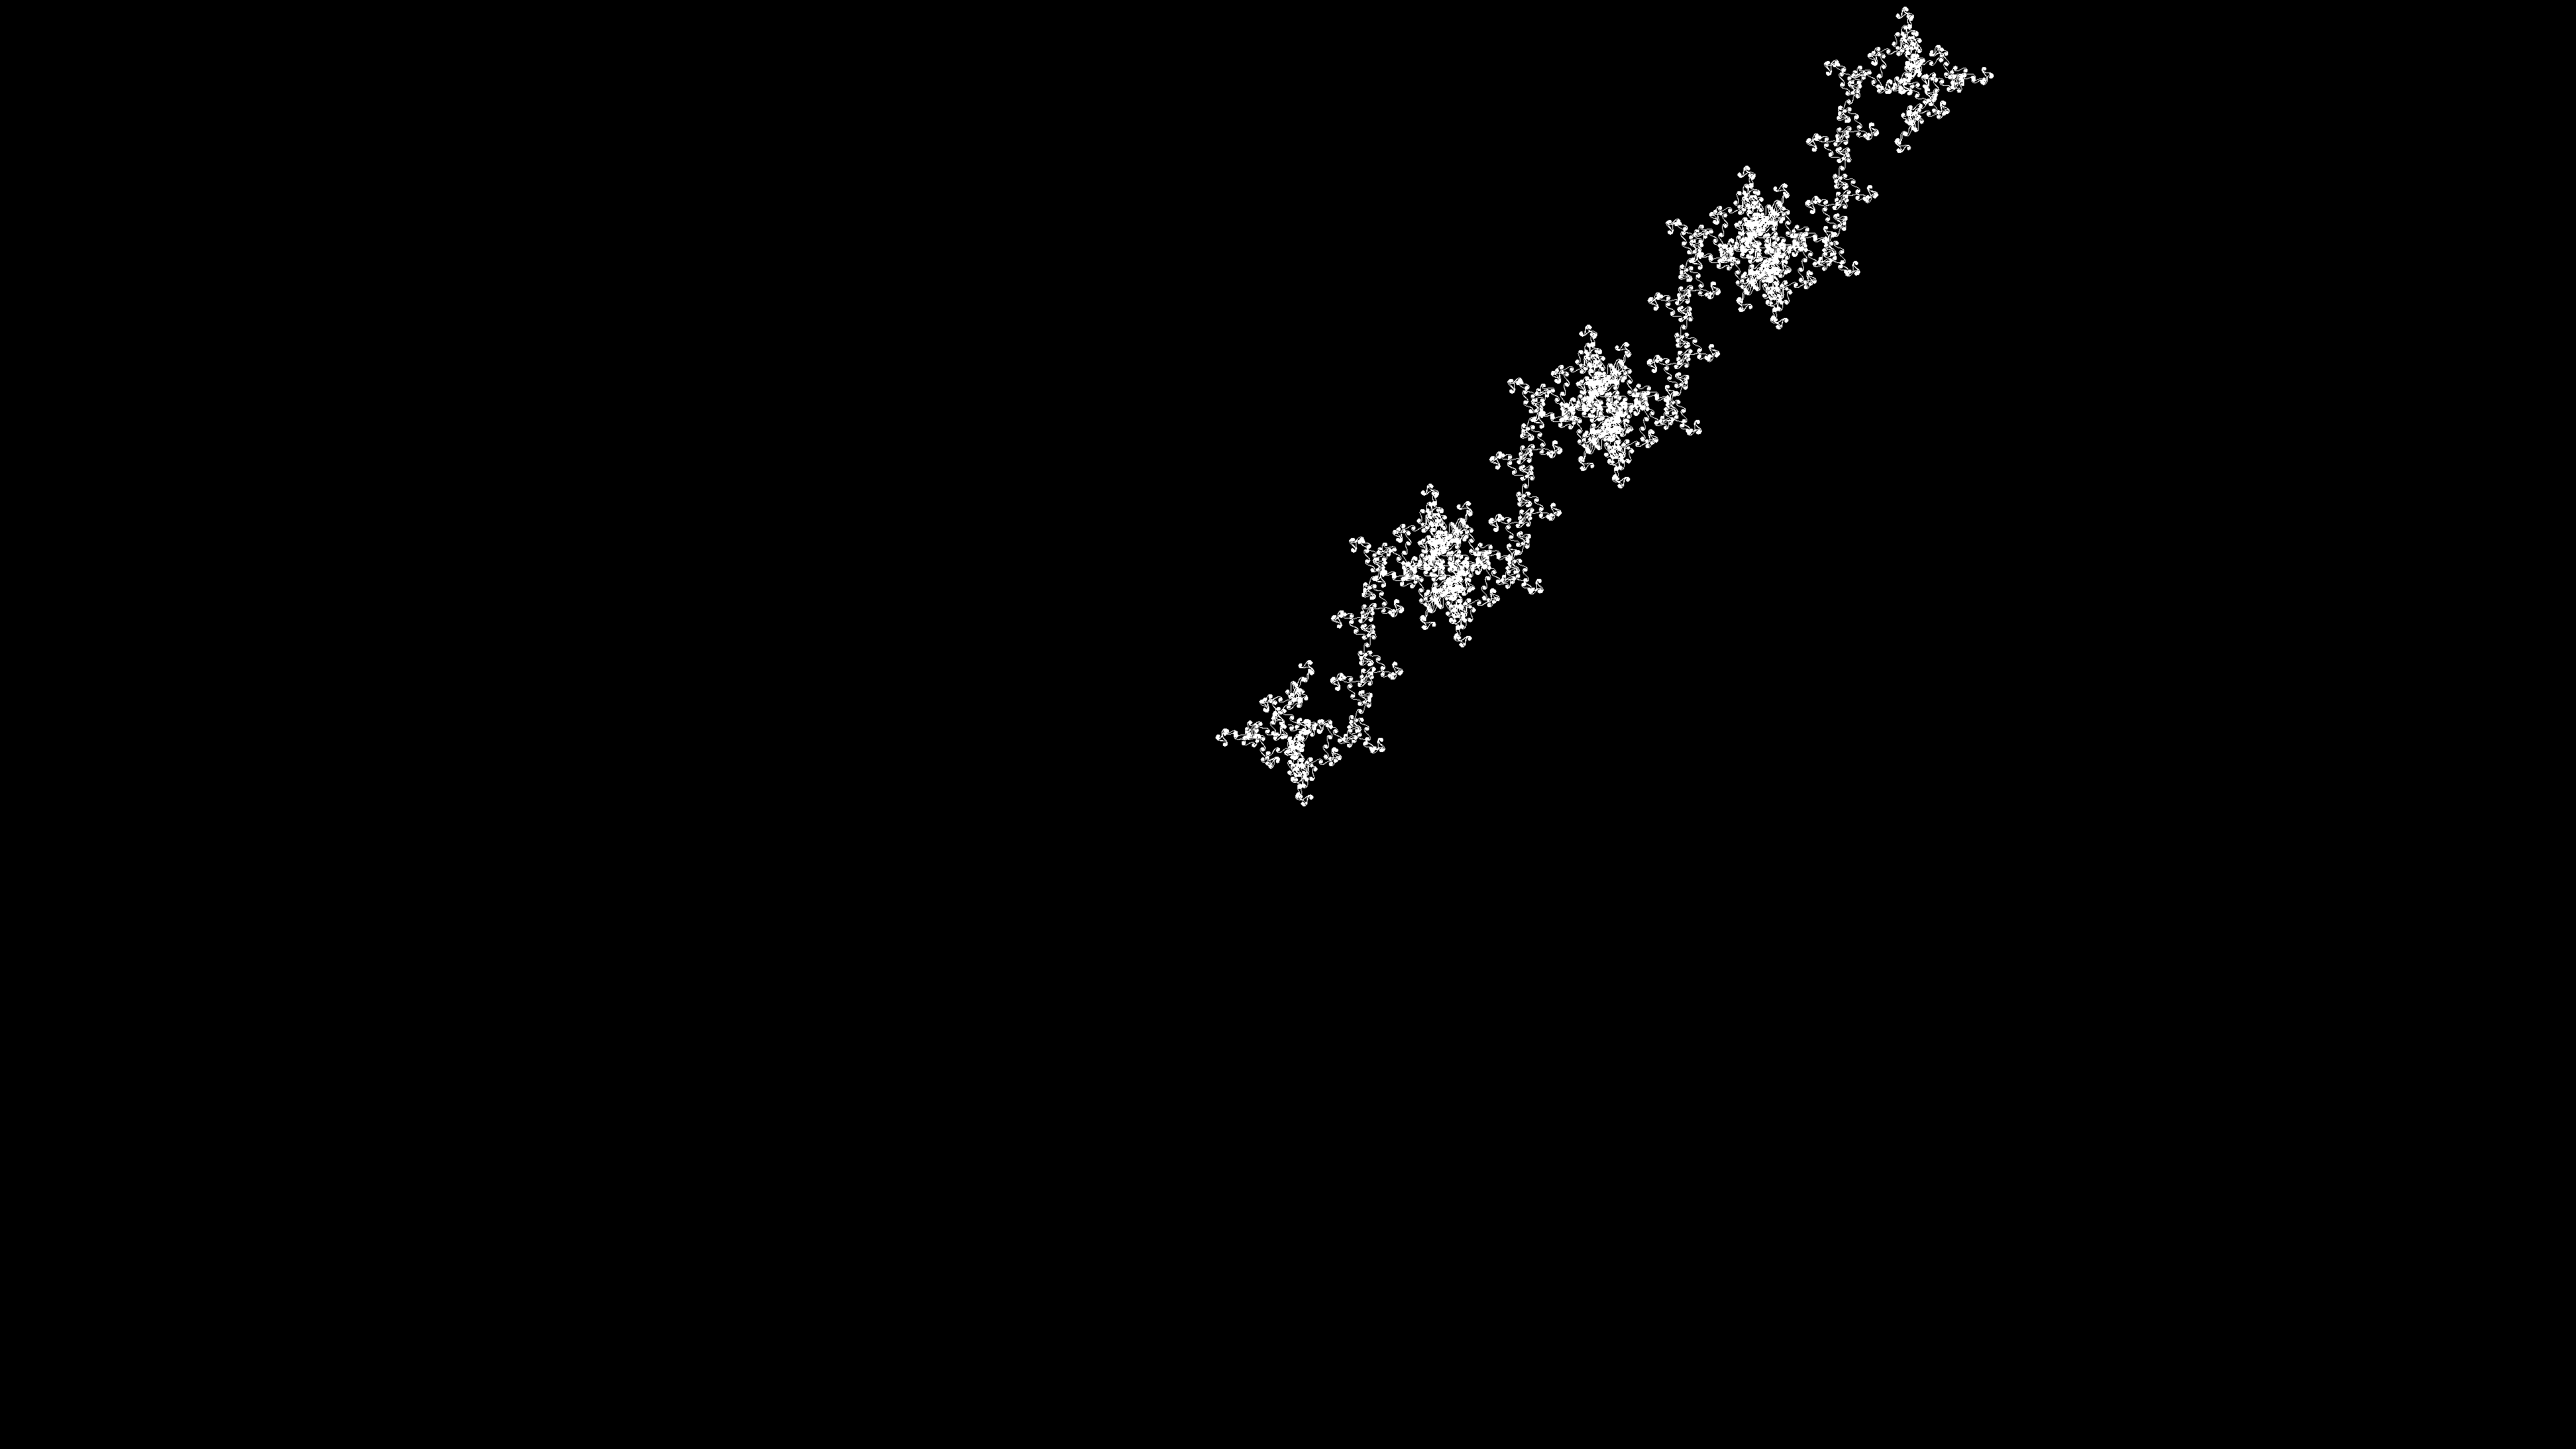
\includegraphics[width=\linewidth]{./stepsplusoneimages/0000000060.png}
    \caption{tf p=499 q=200157 theta=000 89749547.png}
  \end{subfigure}
  \caption{n=058 s=400 s+1=401}
  \label{fig:n=058}
\end{figure}
\begin{figure}[H]
  \centering
  \begin{subfigure}[t]{0.48\textwidth}
    \centering
    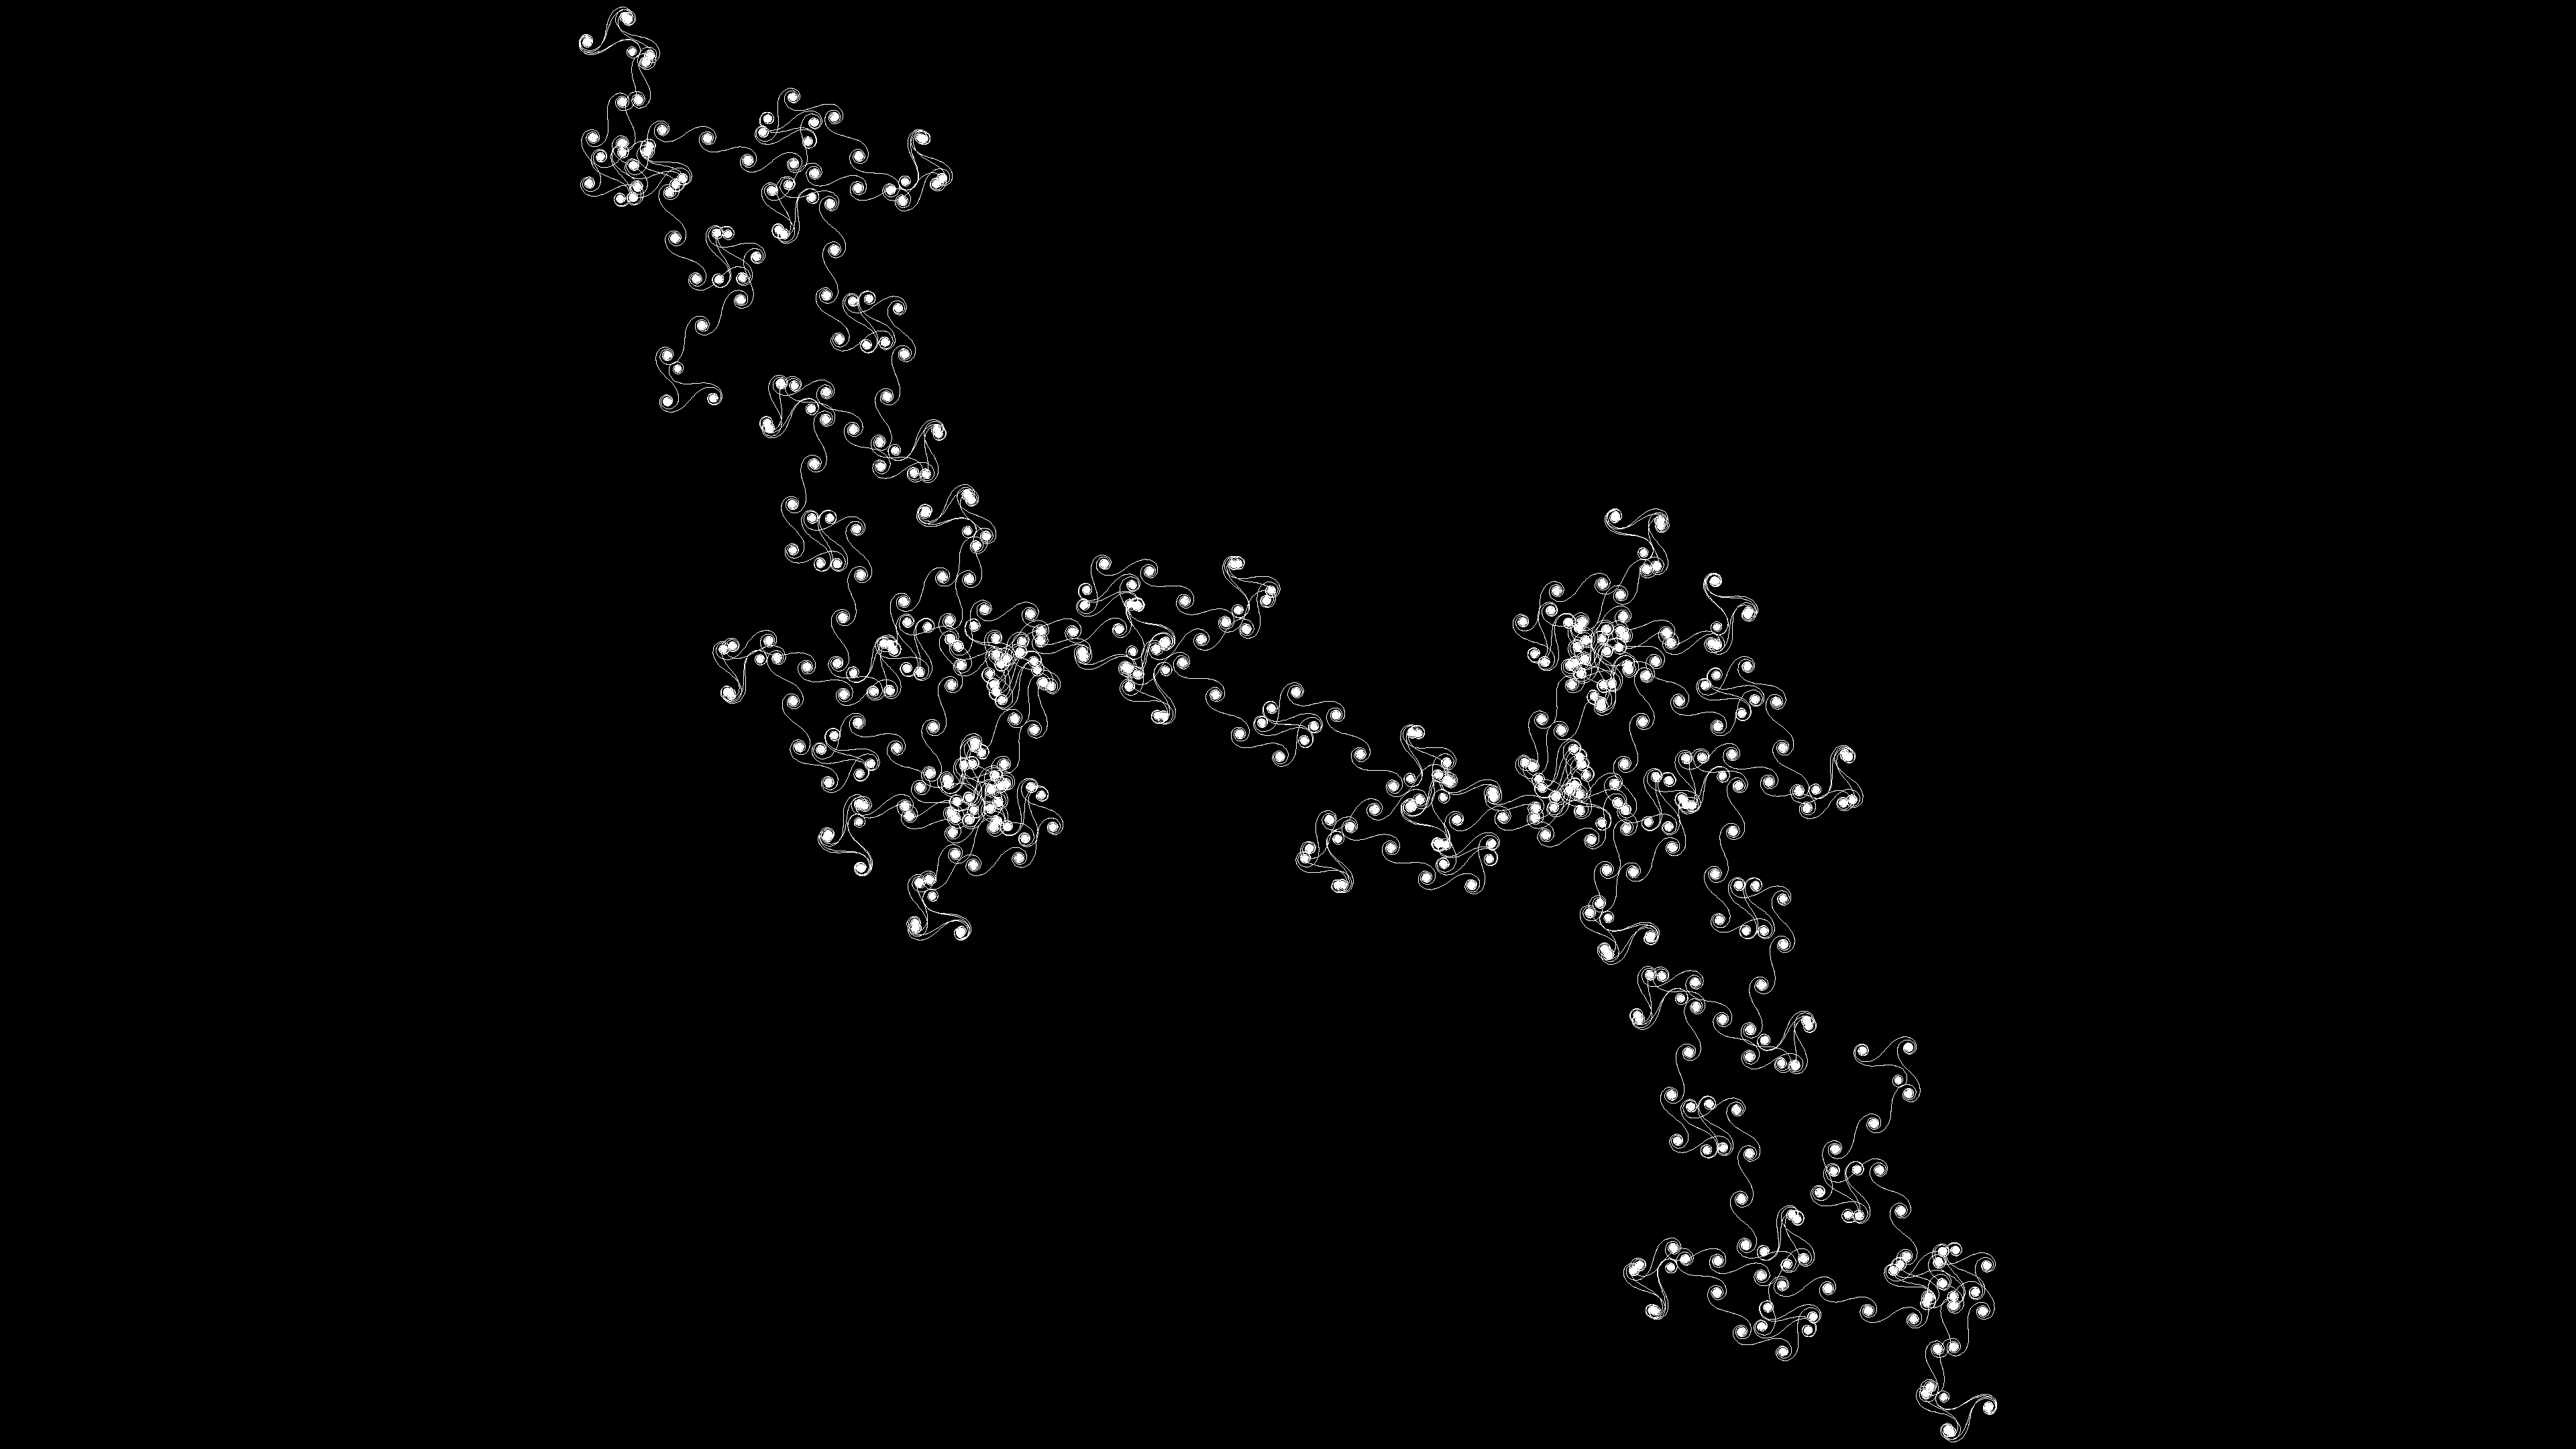
\includegraphics[width=\linewidth]{./stepsplusoneimages/0000000061.png}
    \caption{tf p=499 q=199660 theta=000 89972954.png}
  \end{subfigure}
  \begin{subfigure}[t]{0.48\textwidth}
    \centering
    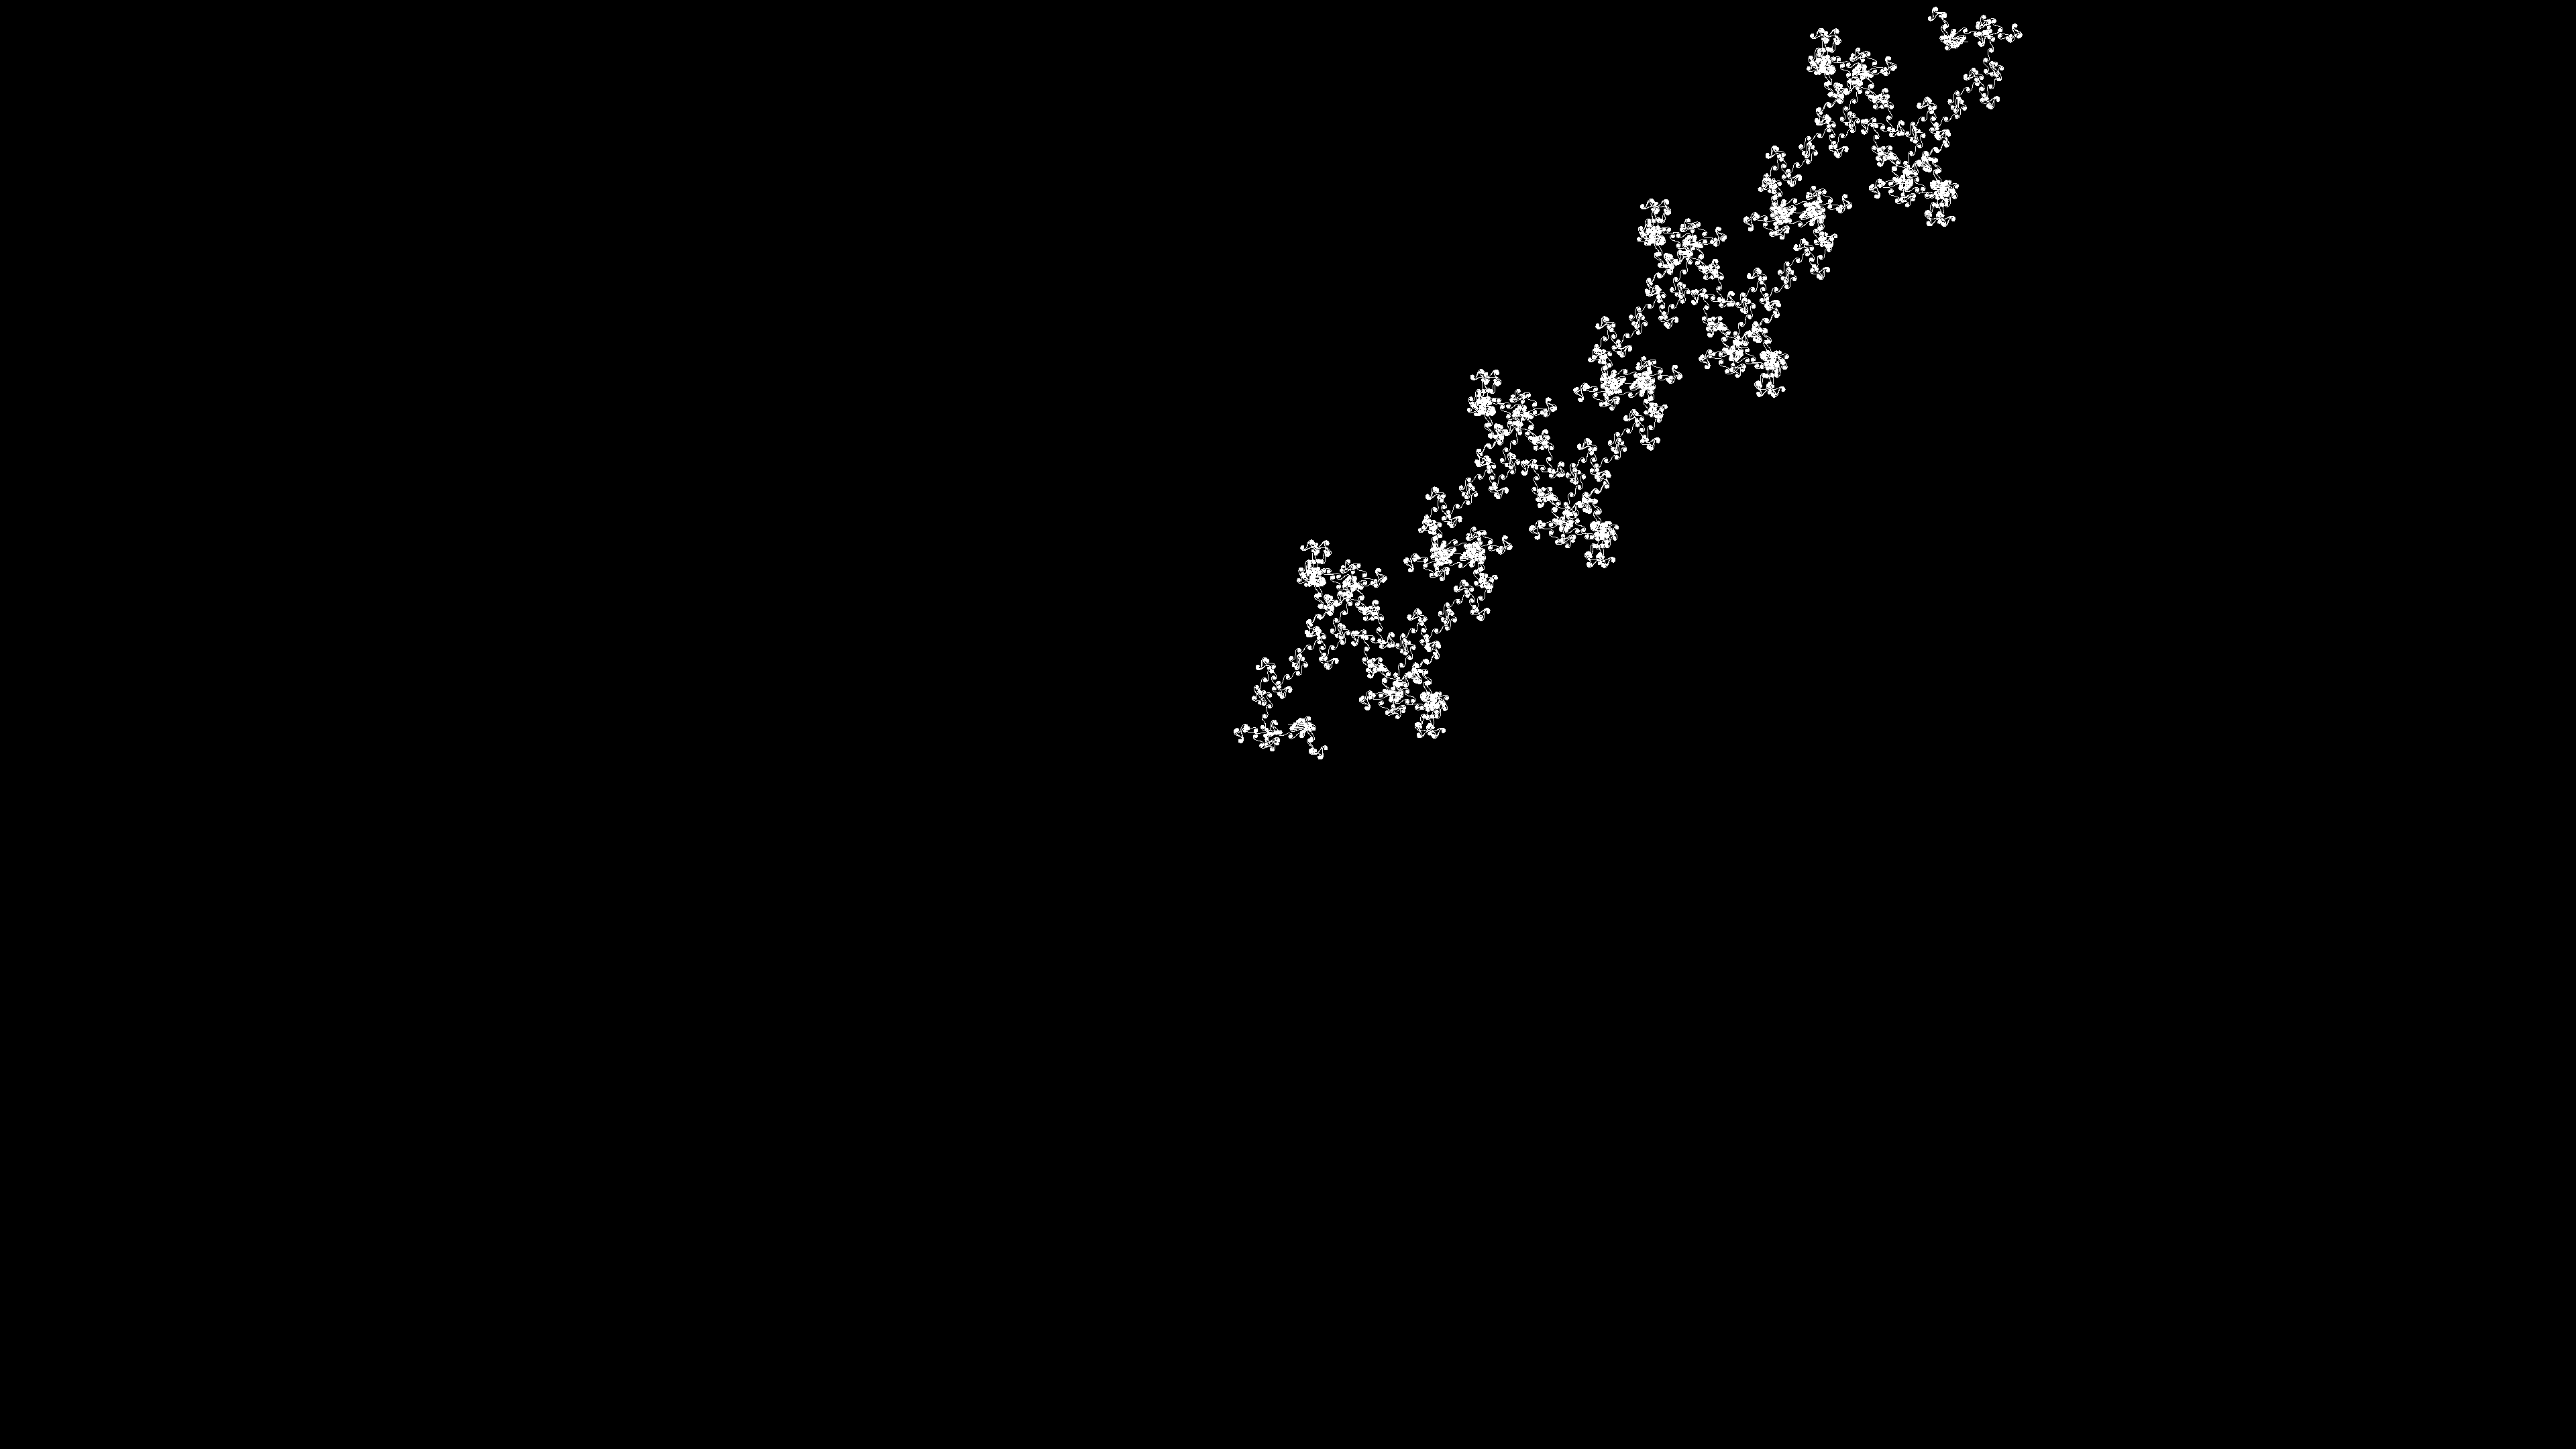
\includegraphics[width=\linewidth]{./stepsplusoneimages/0000000062.png}
    \caption{tf p=499 q=200159 theta=000 89748650.png}
  \end{subfigure}
  \caption{n=060 s=400 s+1=401}
  \label{fig:n=060}
\end{figure}
\begin{figure}[H]
  \centering
  \begin{subfigure}[t]{0.48\textwidth}
    \centering
    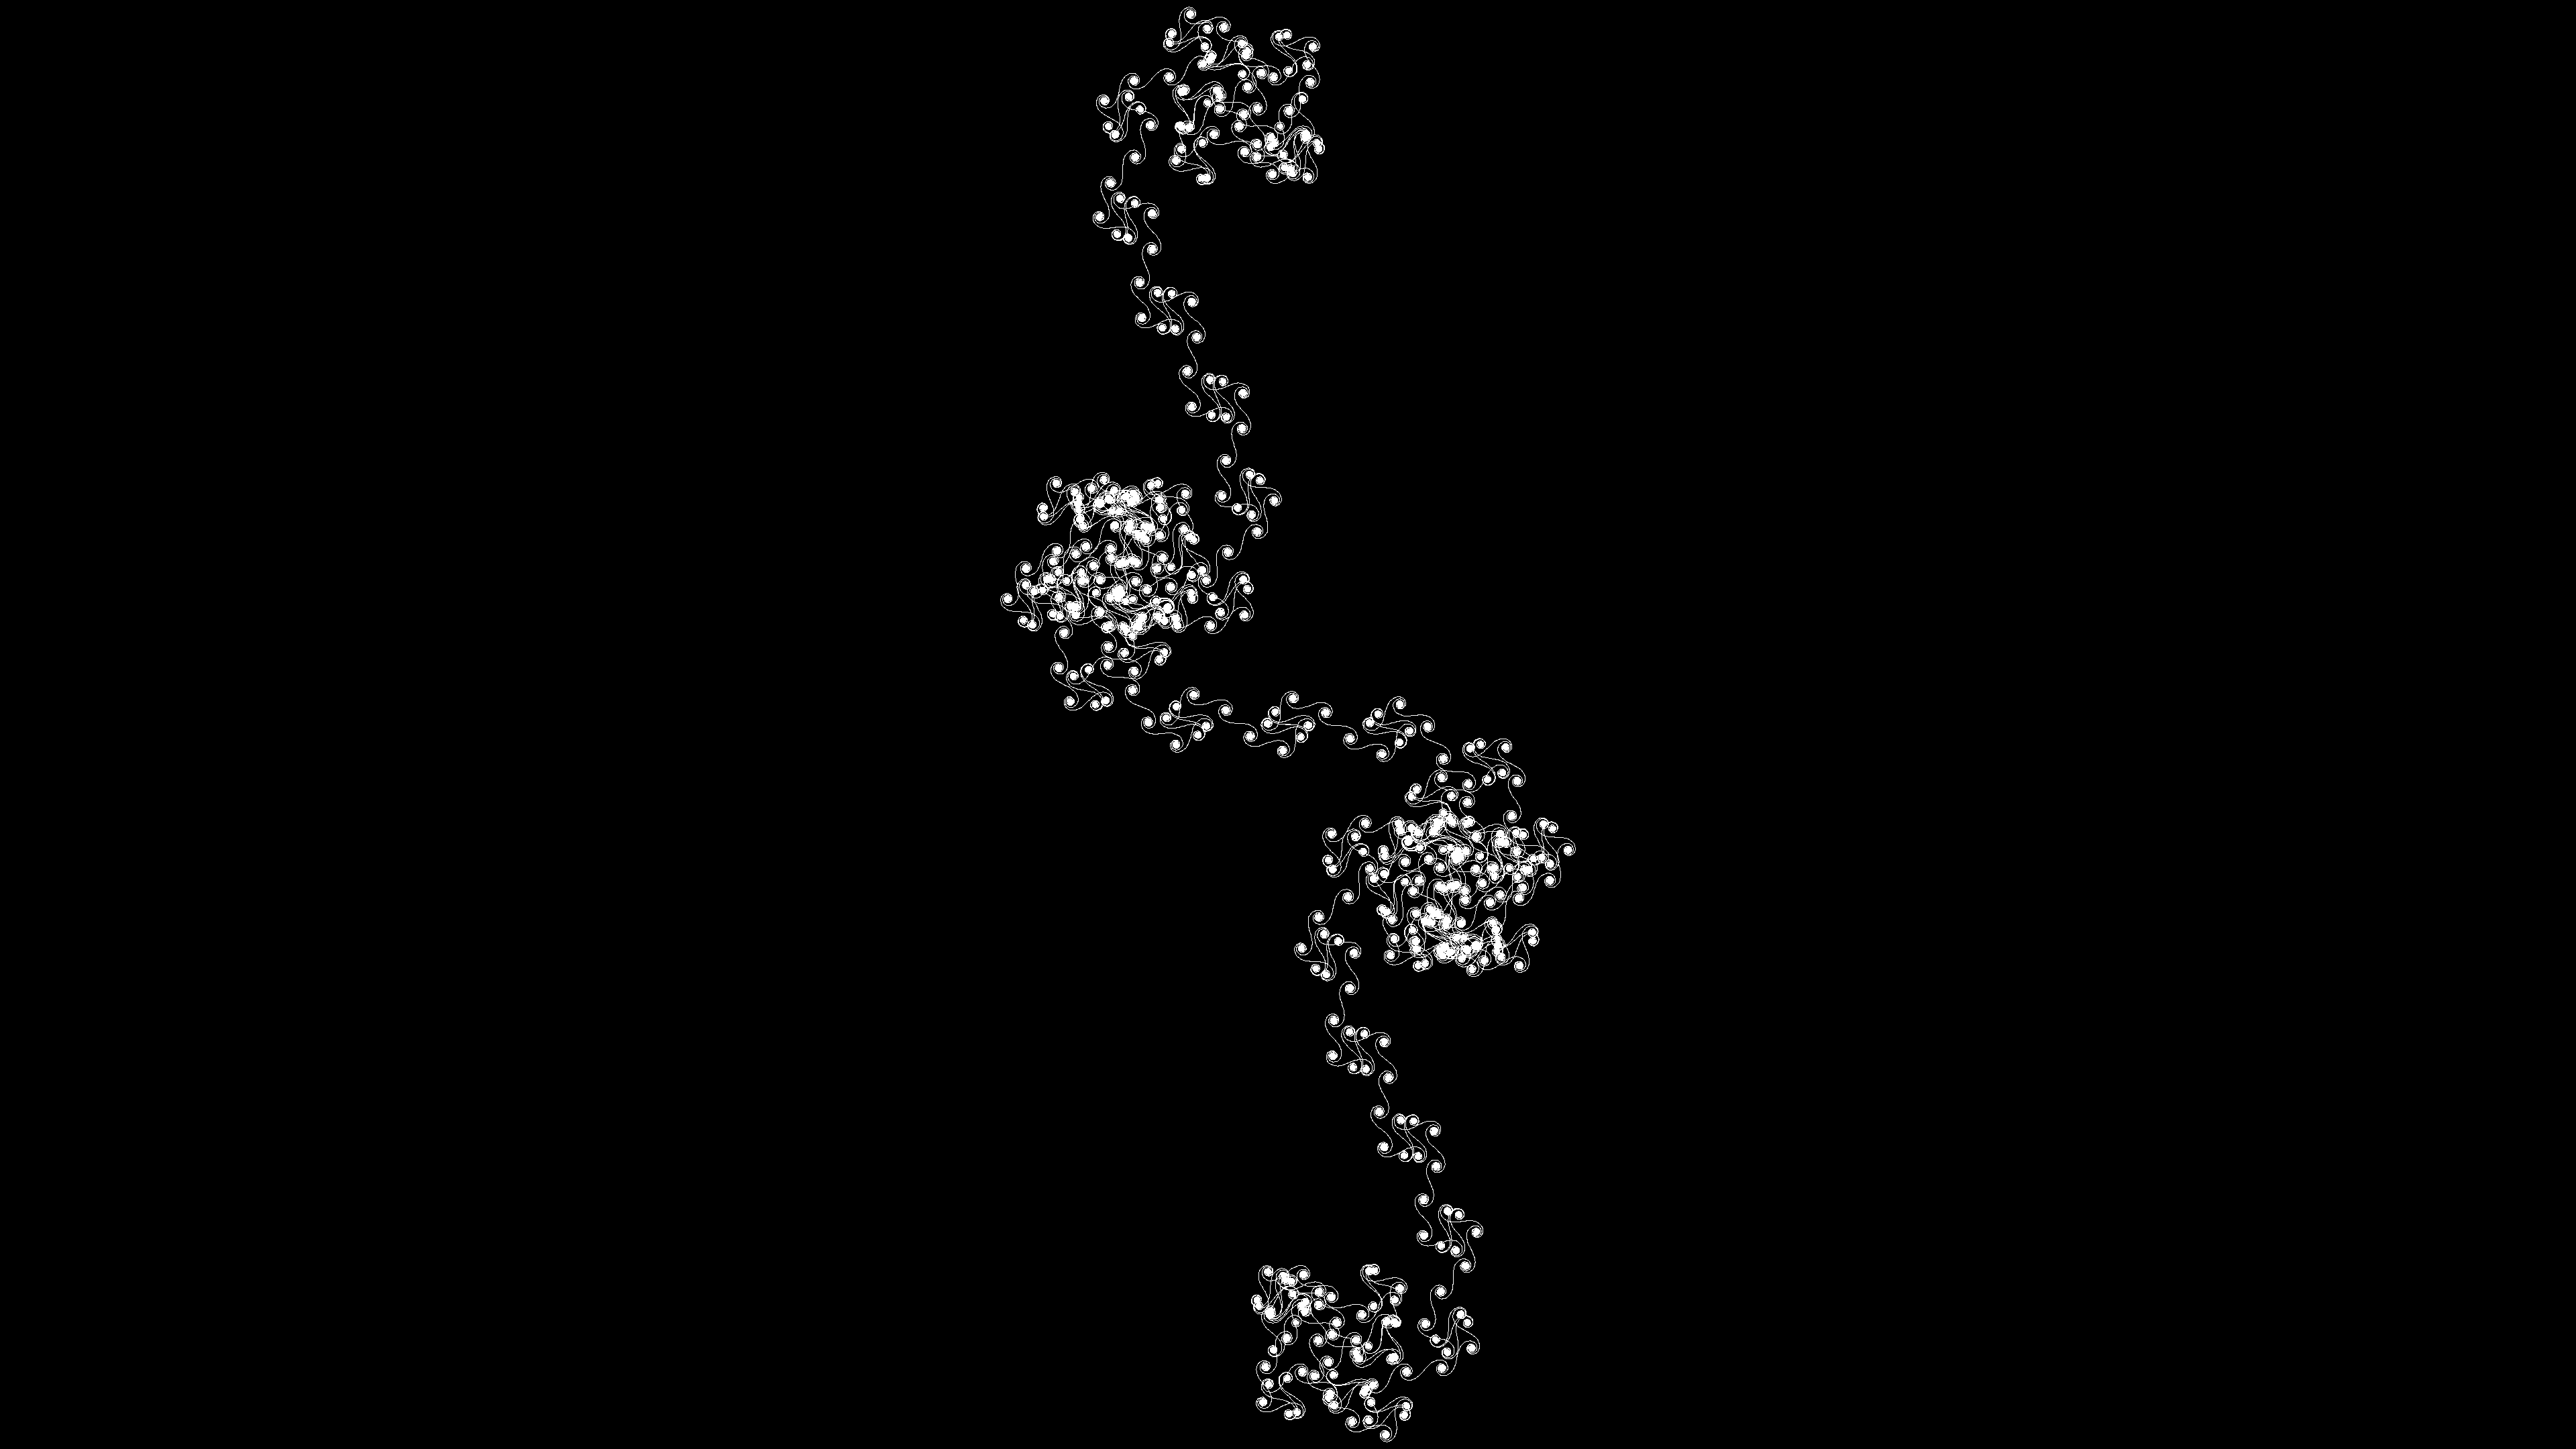
\includegraphics[width=\linewidth]{./stepsplusoneimages/0000000063.png}
    \caption{tf p=499 q=199662 theta=000 89972053.png}
  \end{subfigure}
  \begin{subfigure}[t]{0.48\textwidth}
    \centering
    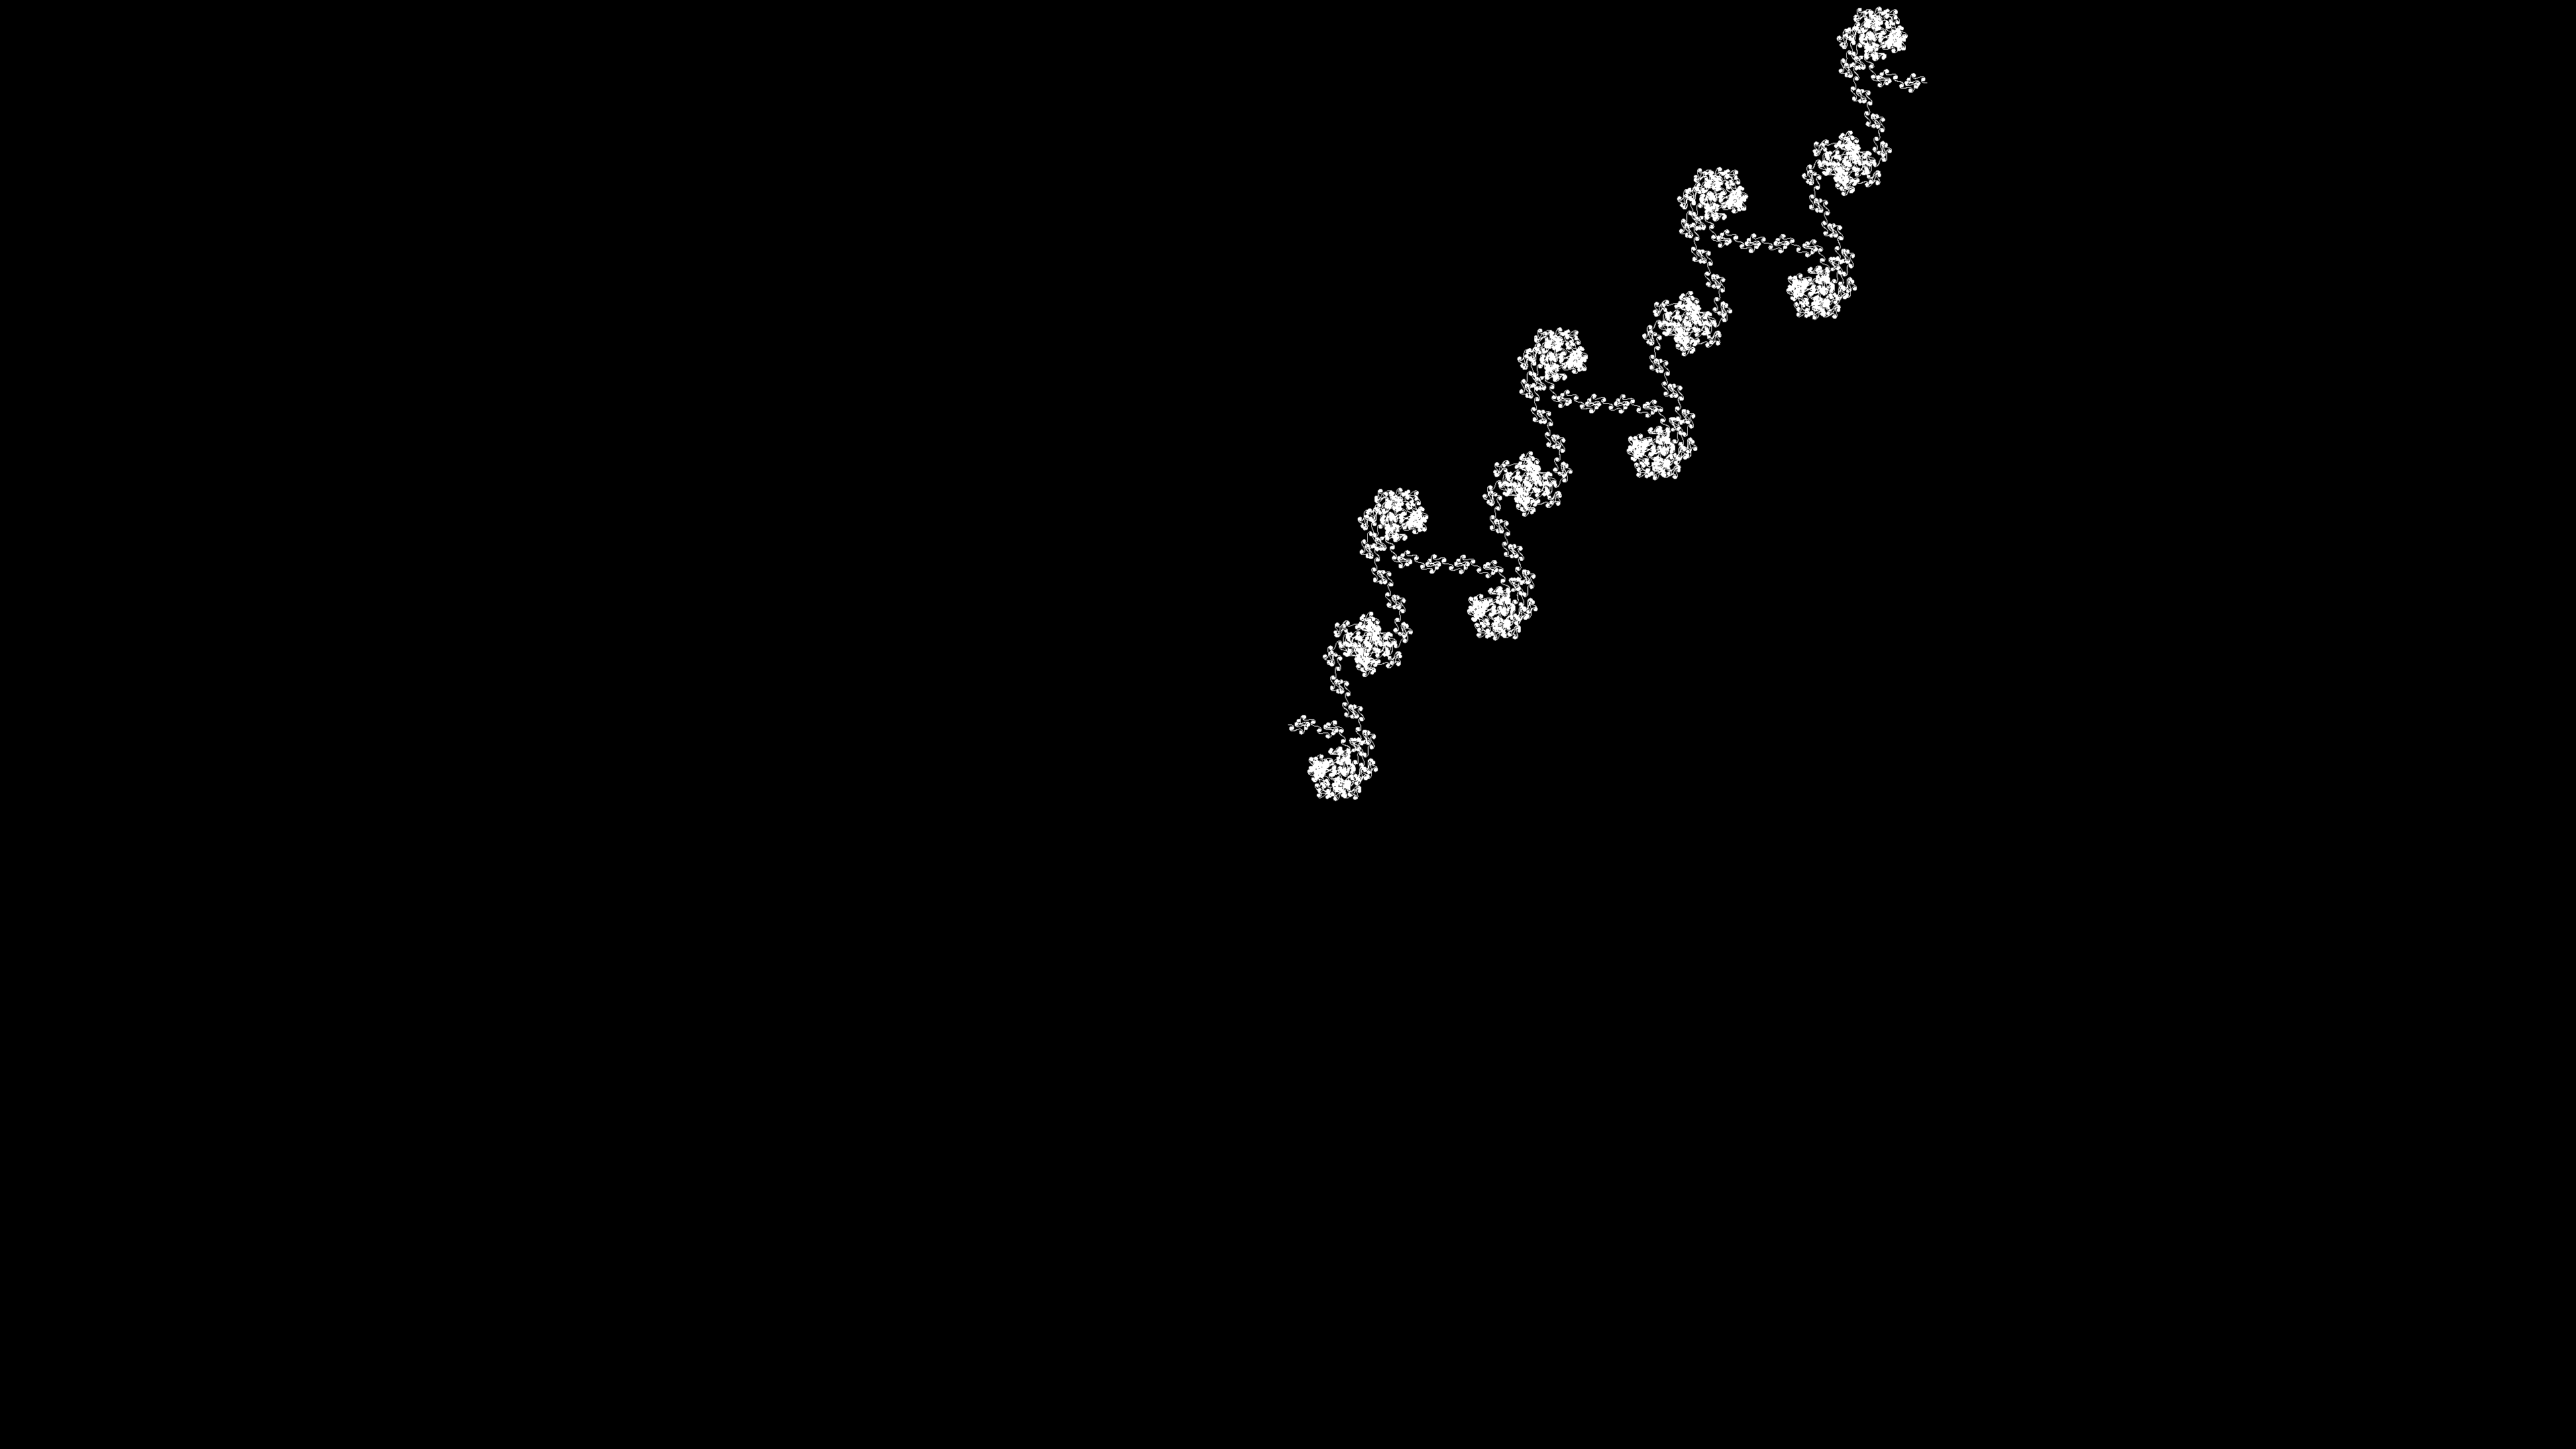
\includegraphics[width=\linewidth]{./stepsplusoneimages/0000000064.png}
    \caption{tf p=499 q=200161 theta=000 89747753.png}
  \end{subfigure}
  \caption{n=062 s=400 s+1=401}
  \label{fig:n=062}
\end{figure}
\begin{figure}[H]
  \centering
  \begin{subfigure}[t]{0.48\textwidth}
    \centering
    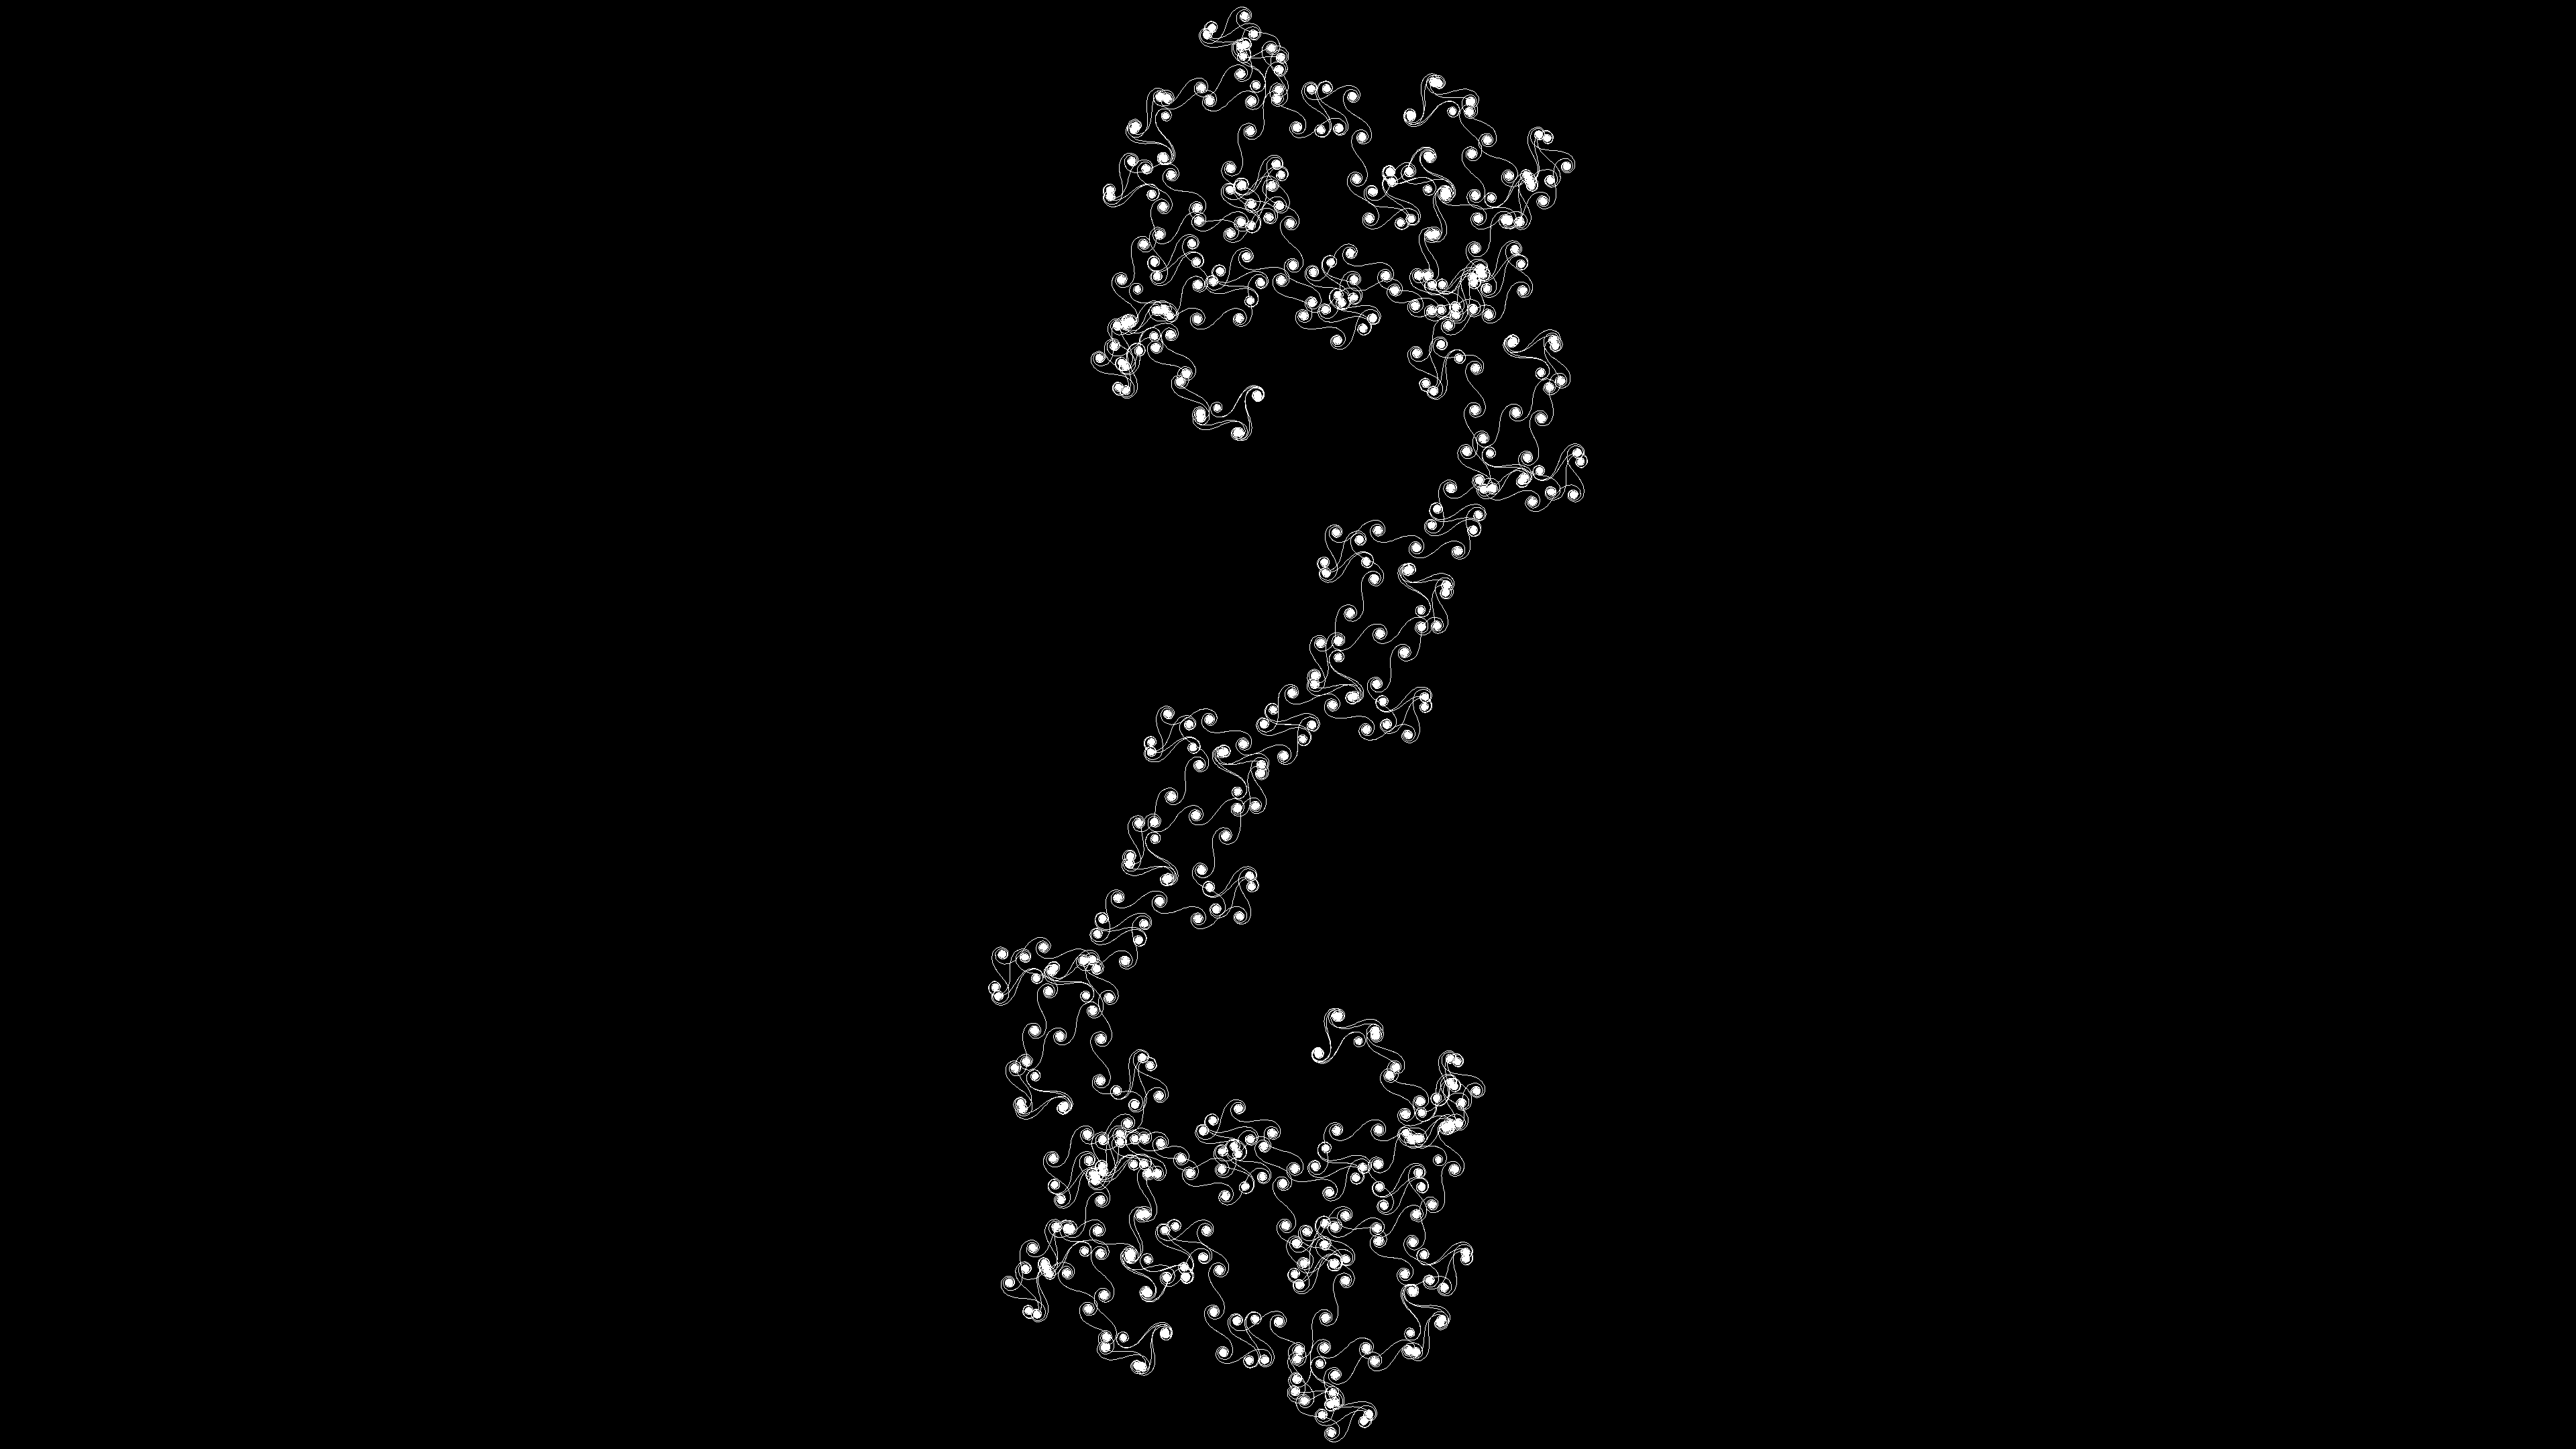
\includegraphics[width=\linewidth]{./stepsplusoneimages/0000000065.png}
    \caption{tf p=499 q=199664 theta=000 89971152.png}
  \end{subfigure}
  \begin{subfigure}[t]{0.48\textwidth}
    \centering
    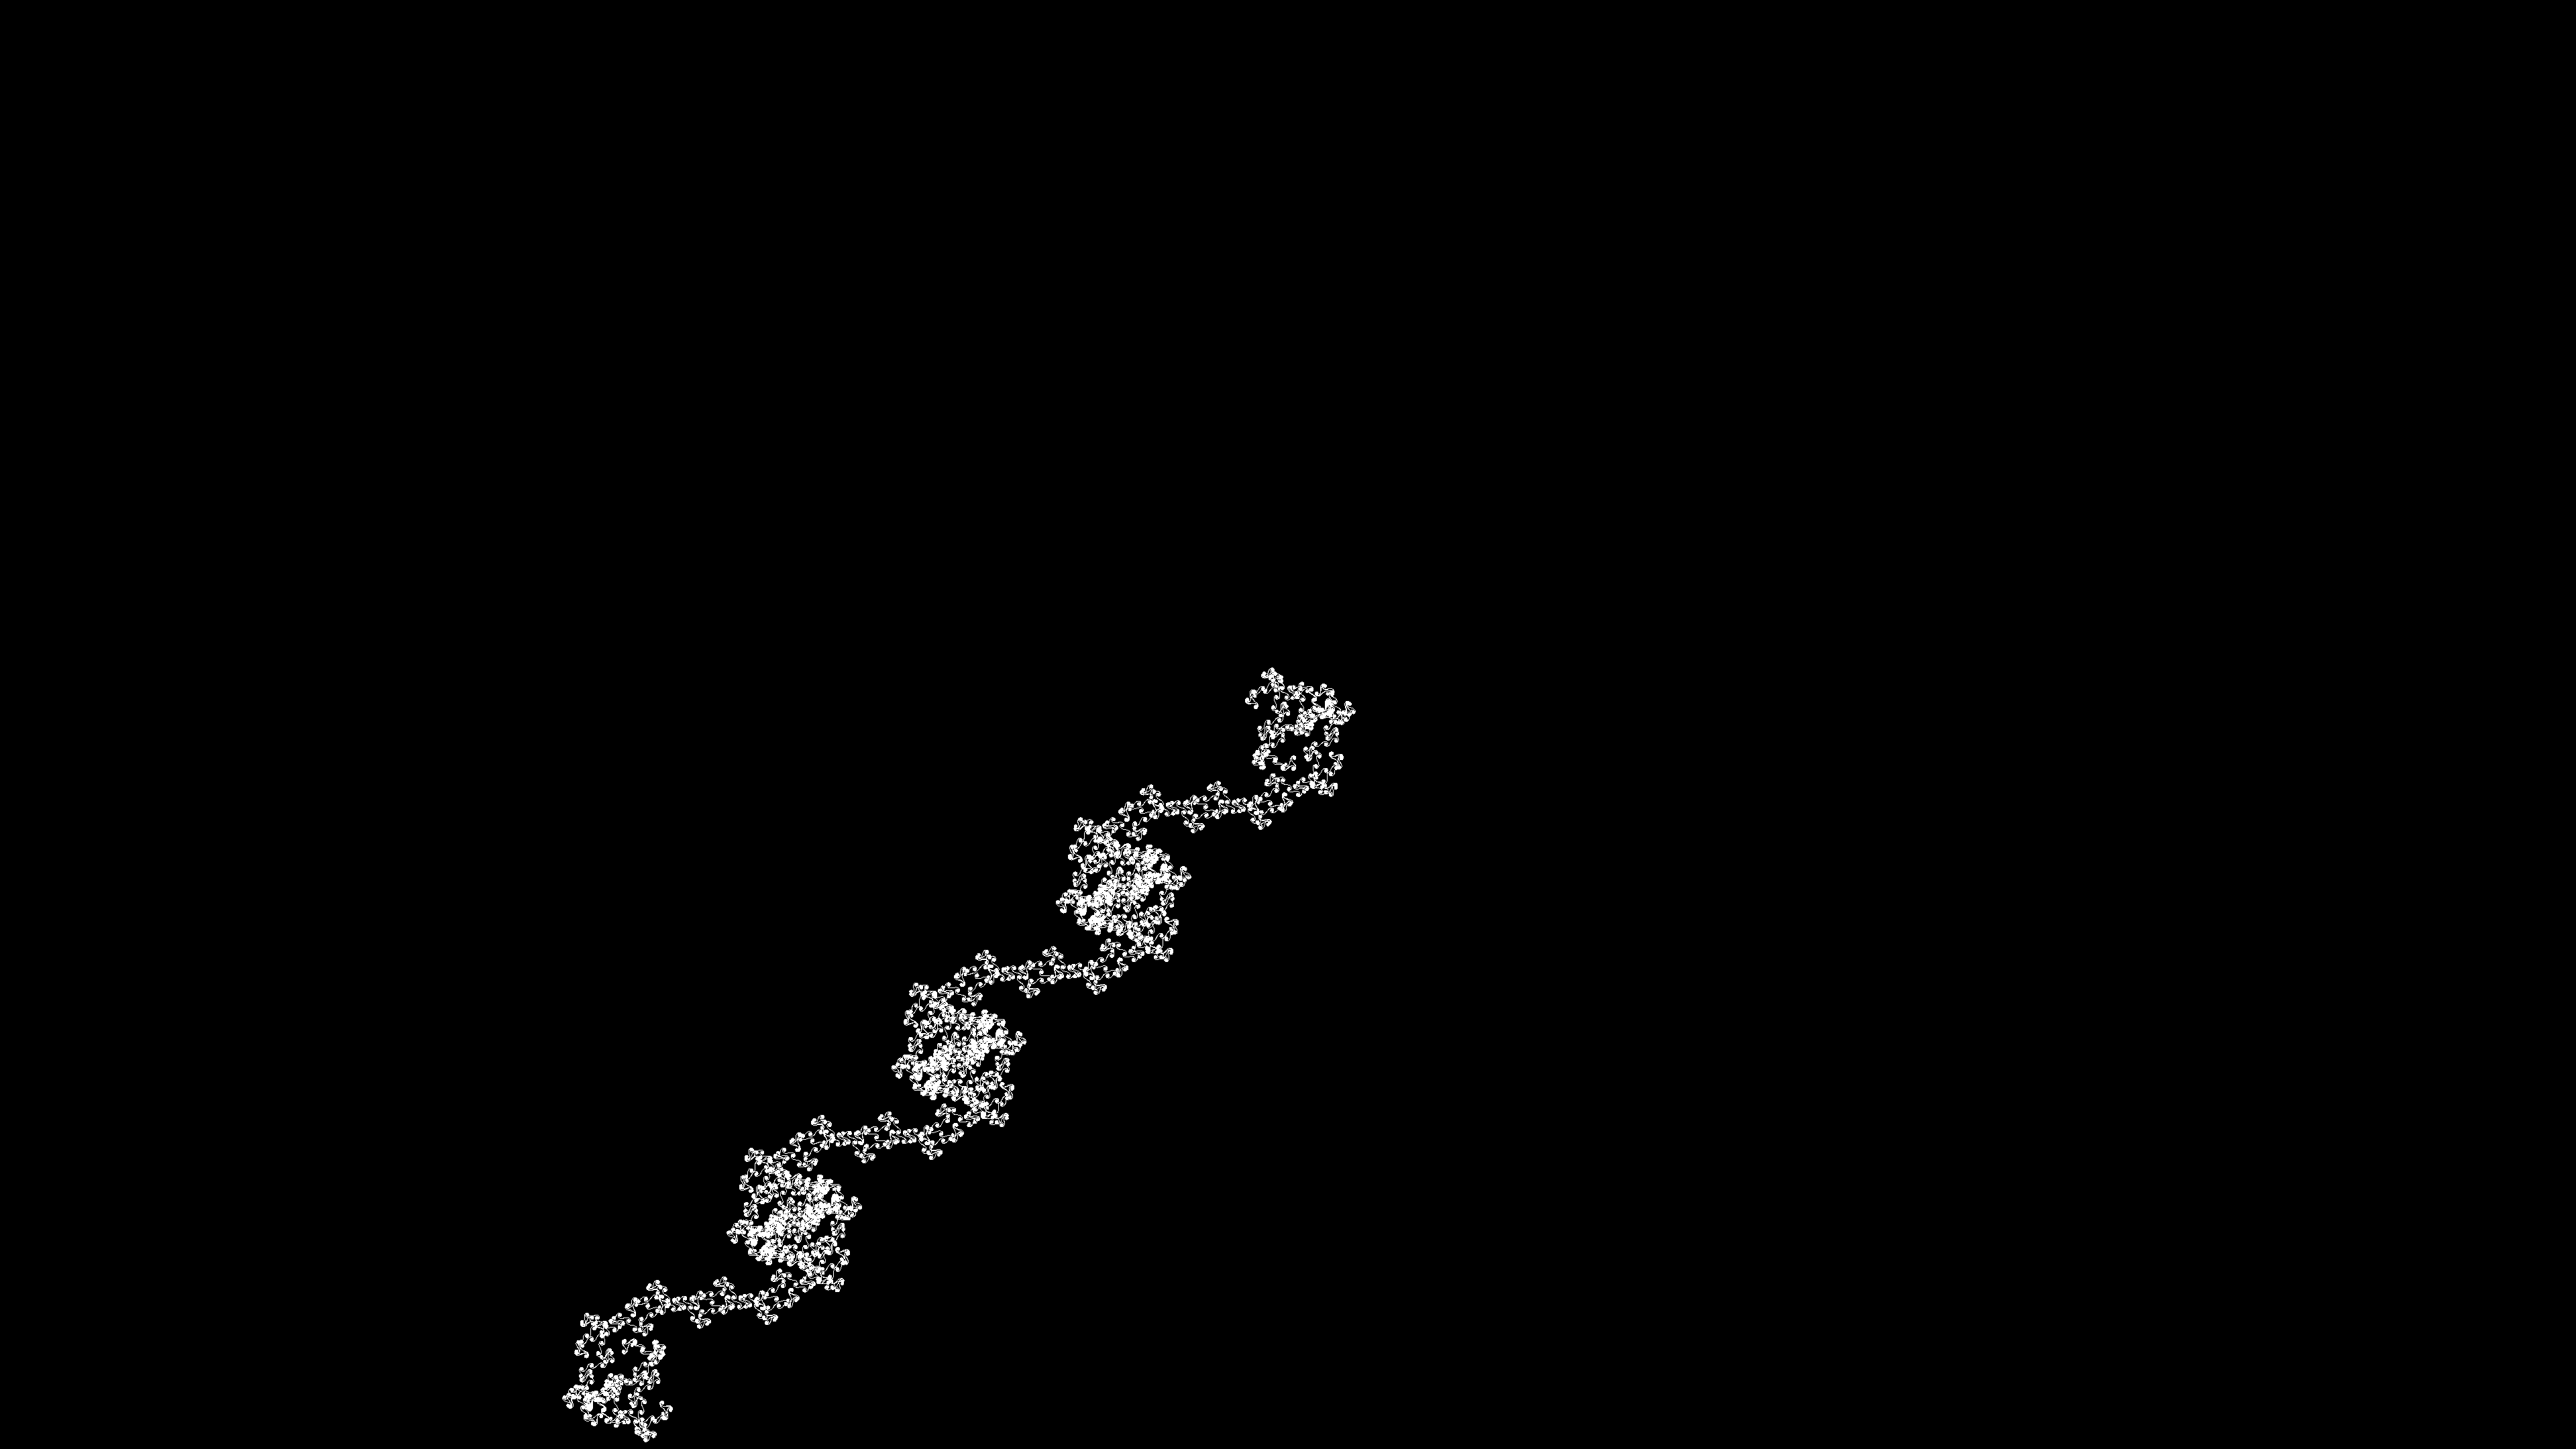
\includegraphics[width=\linewidth]{./stepsplusoneimages/0000000066.png}
    \caption{tf p=499 q=200163 theta=000 89746856.png}
  \end{subfigure}
  \caption{n=064 s=400 s+1=401}
  \label{fig:n=064}
\end{figure}
\begin{figure}[H]
  \centering
  \begin{subfigure}[t]{0.48\textwidth}
    \centering
    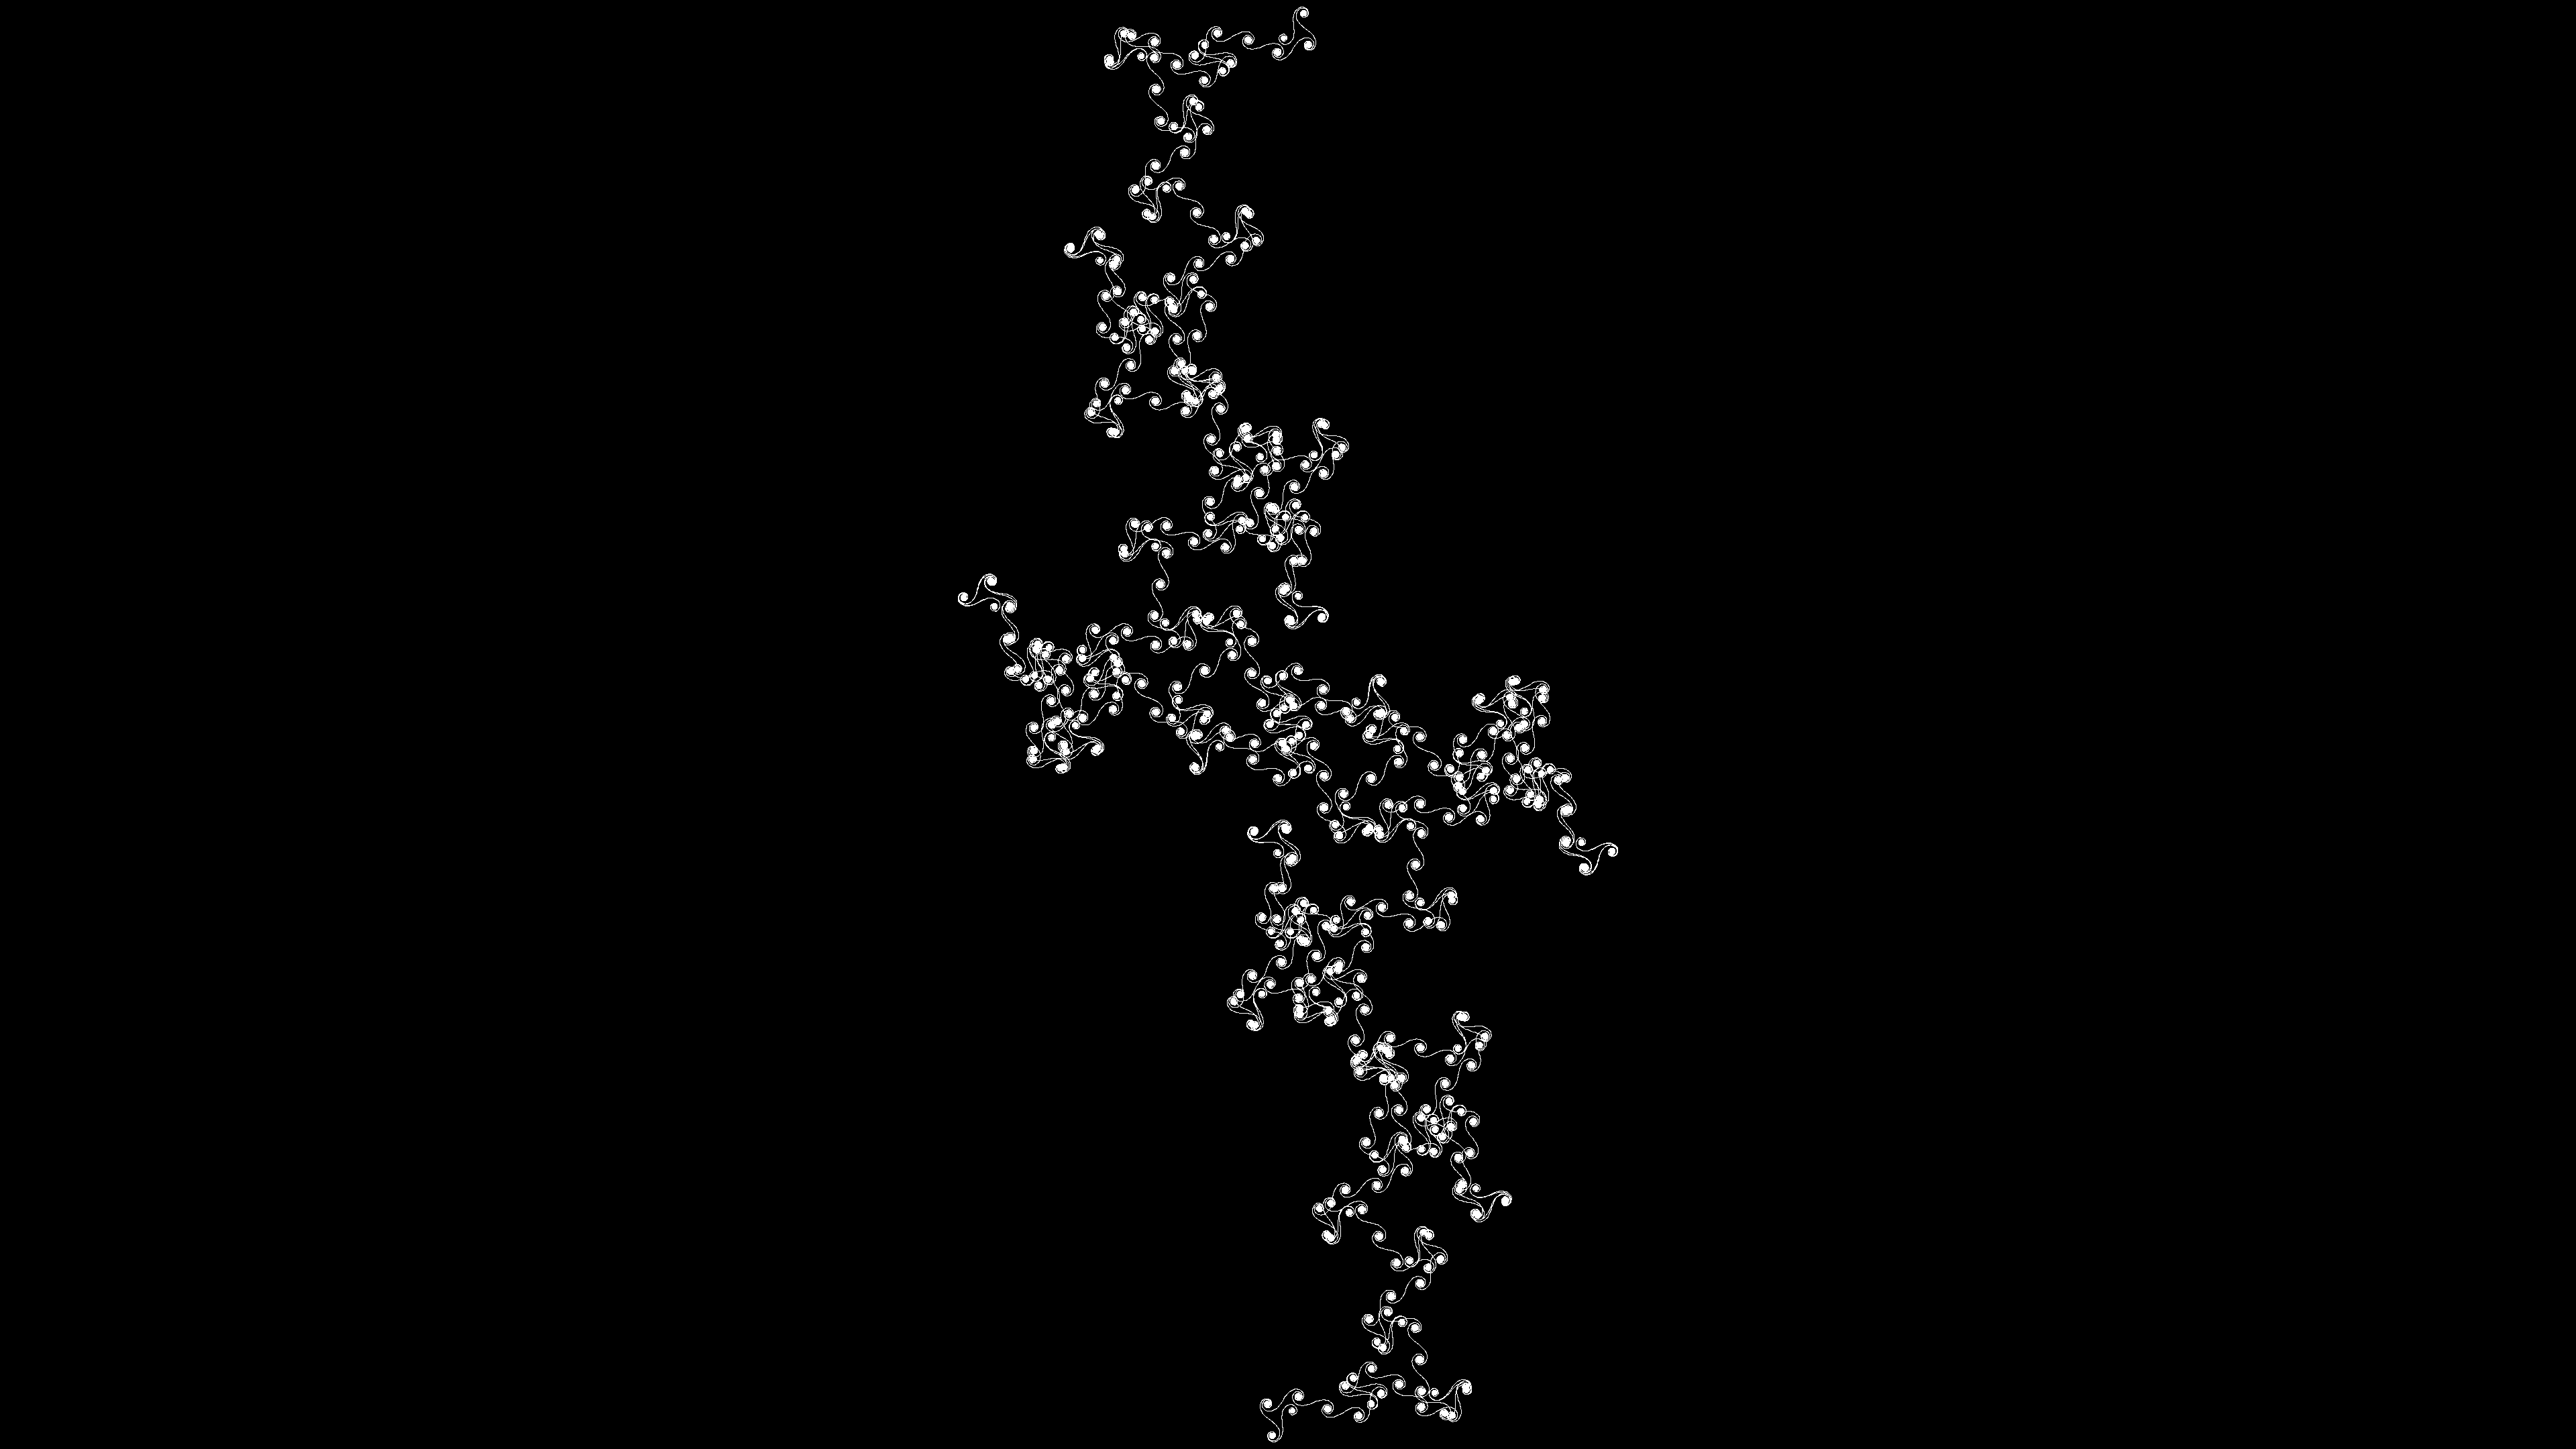
\includegraphics[width=\linewidth]{./stepsplusoneimages/0000000067.png}
    \caption{tf p=499 q=199666 theta=000 89970250.png}
  \end{subfigure}
  \begin{subfigure}[t]{0.48\textwidth}
    \centering
    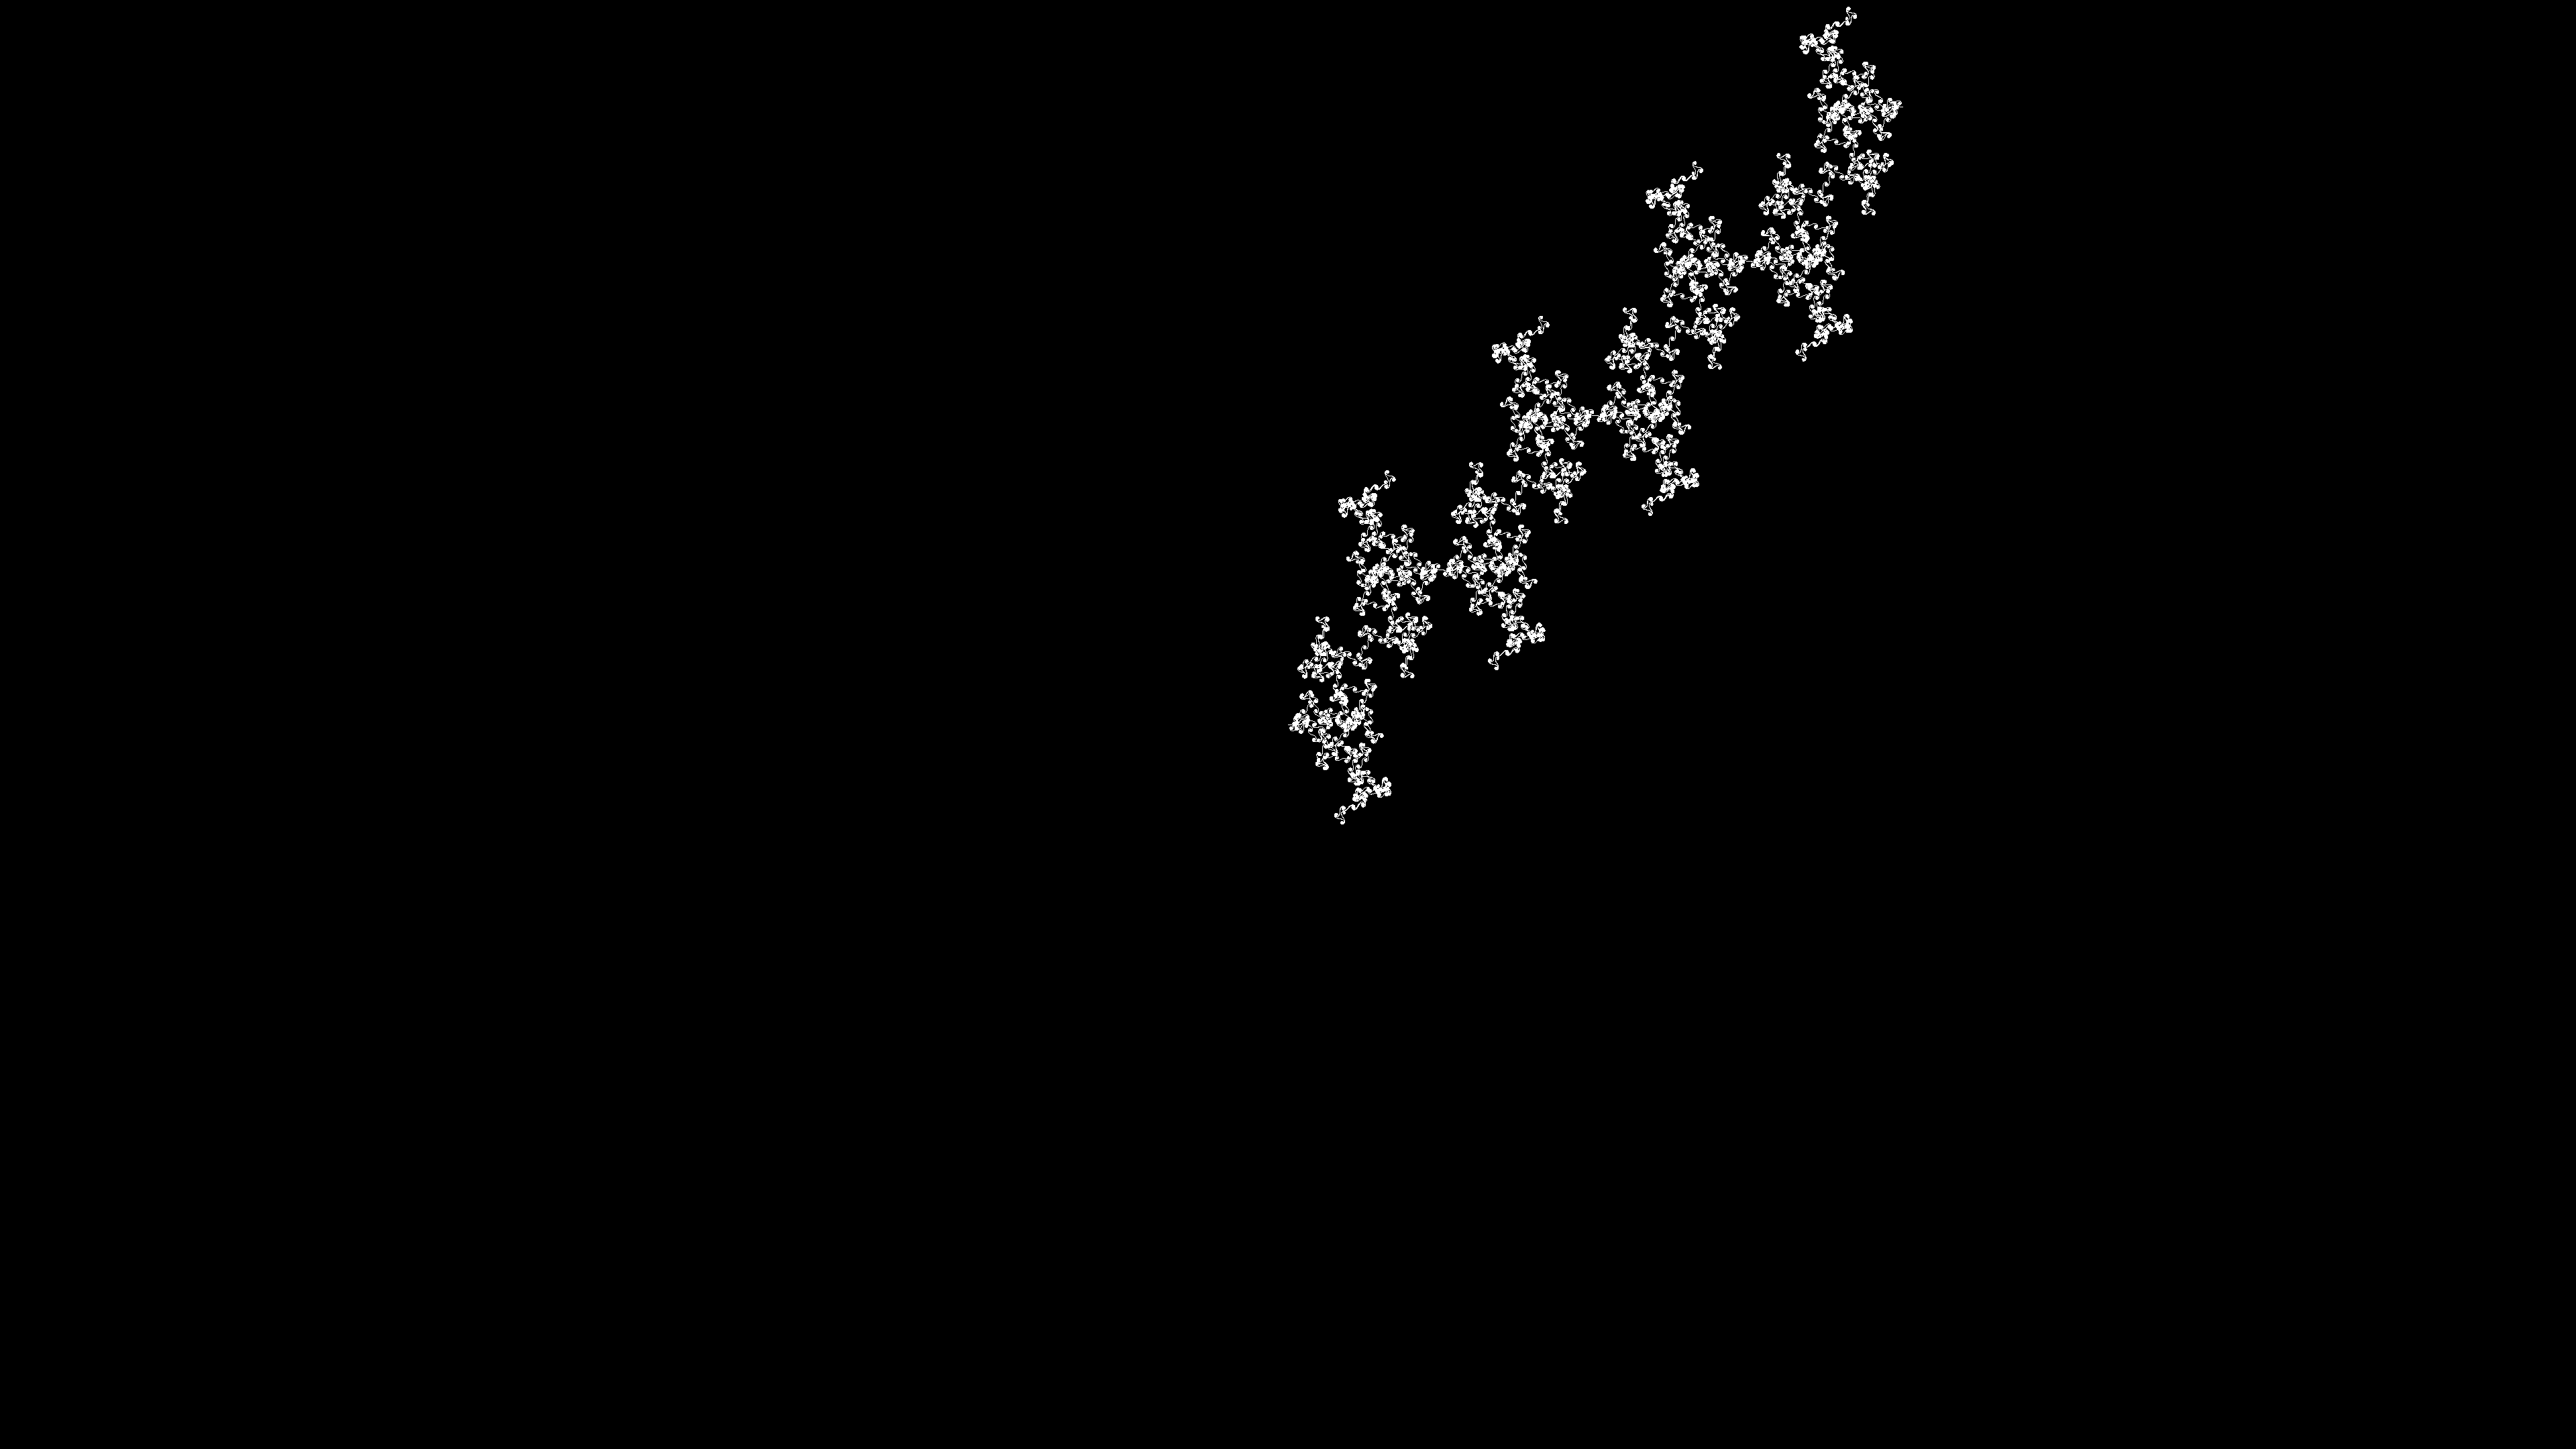
\includegraphics[width=\linewidth]{./stepsplusoneimages/0000000068.png}
    \caption{tf p=499 q=200165 theta=000 89745960.png}
  \end{subfigure}
  \caption{n=066 s=400 s+1=401}
  \label{fig:n=066}
\end{figure}
\begin{figure}[H]
  \centering
  \begin{subfigure}[t]{0.48\textwidth}
    \centering
    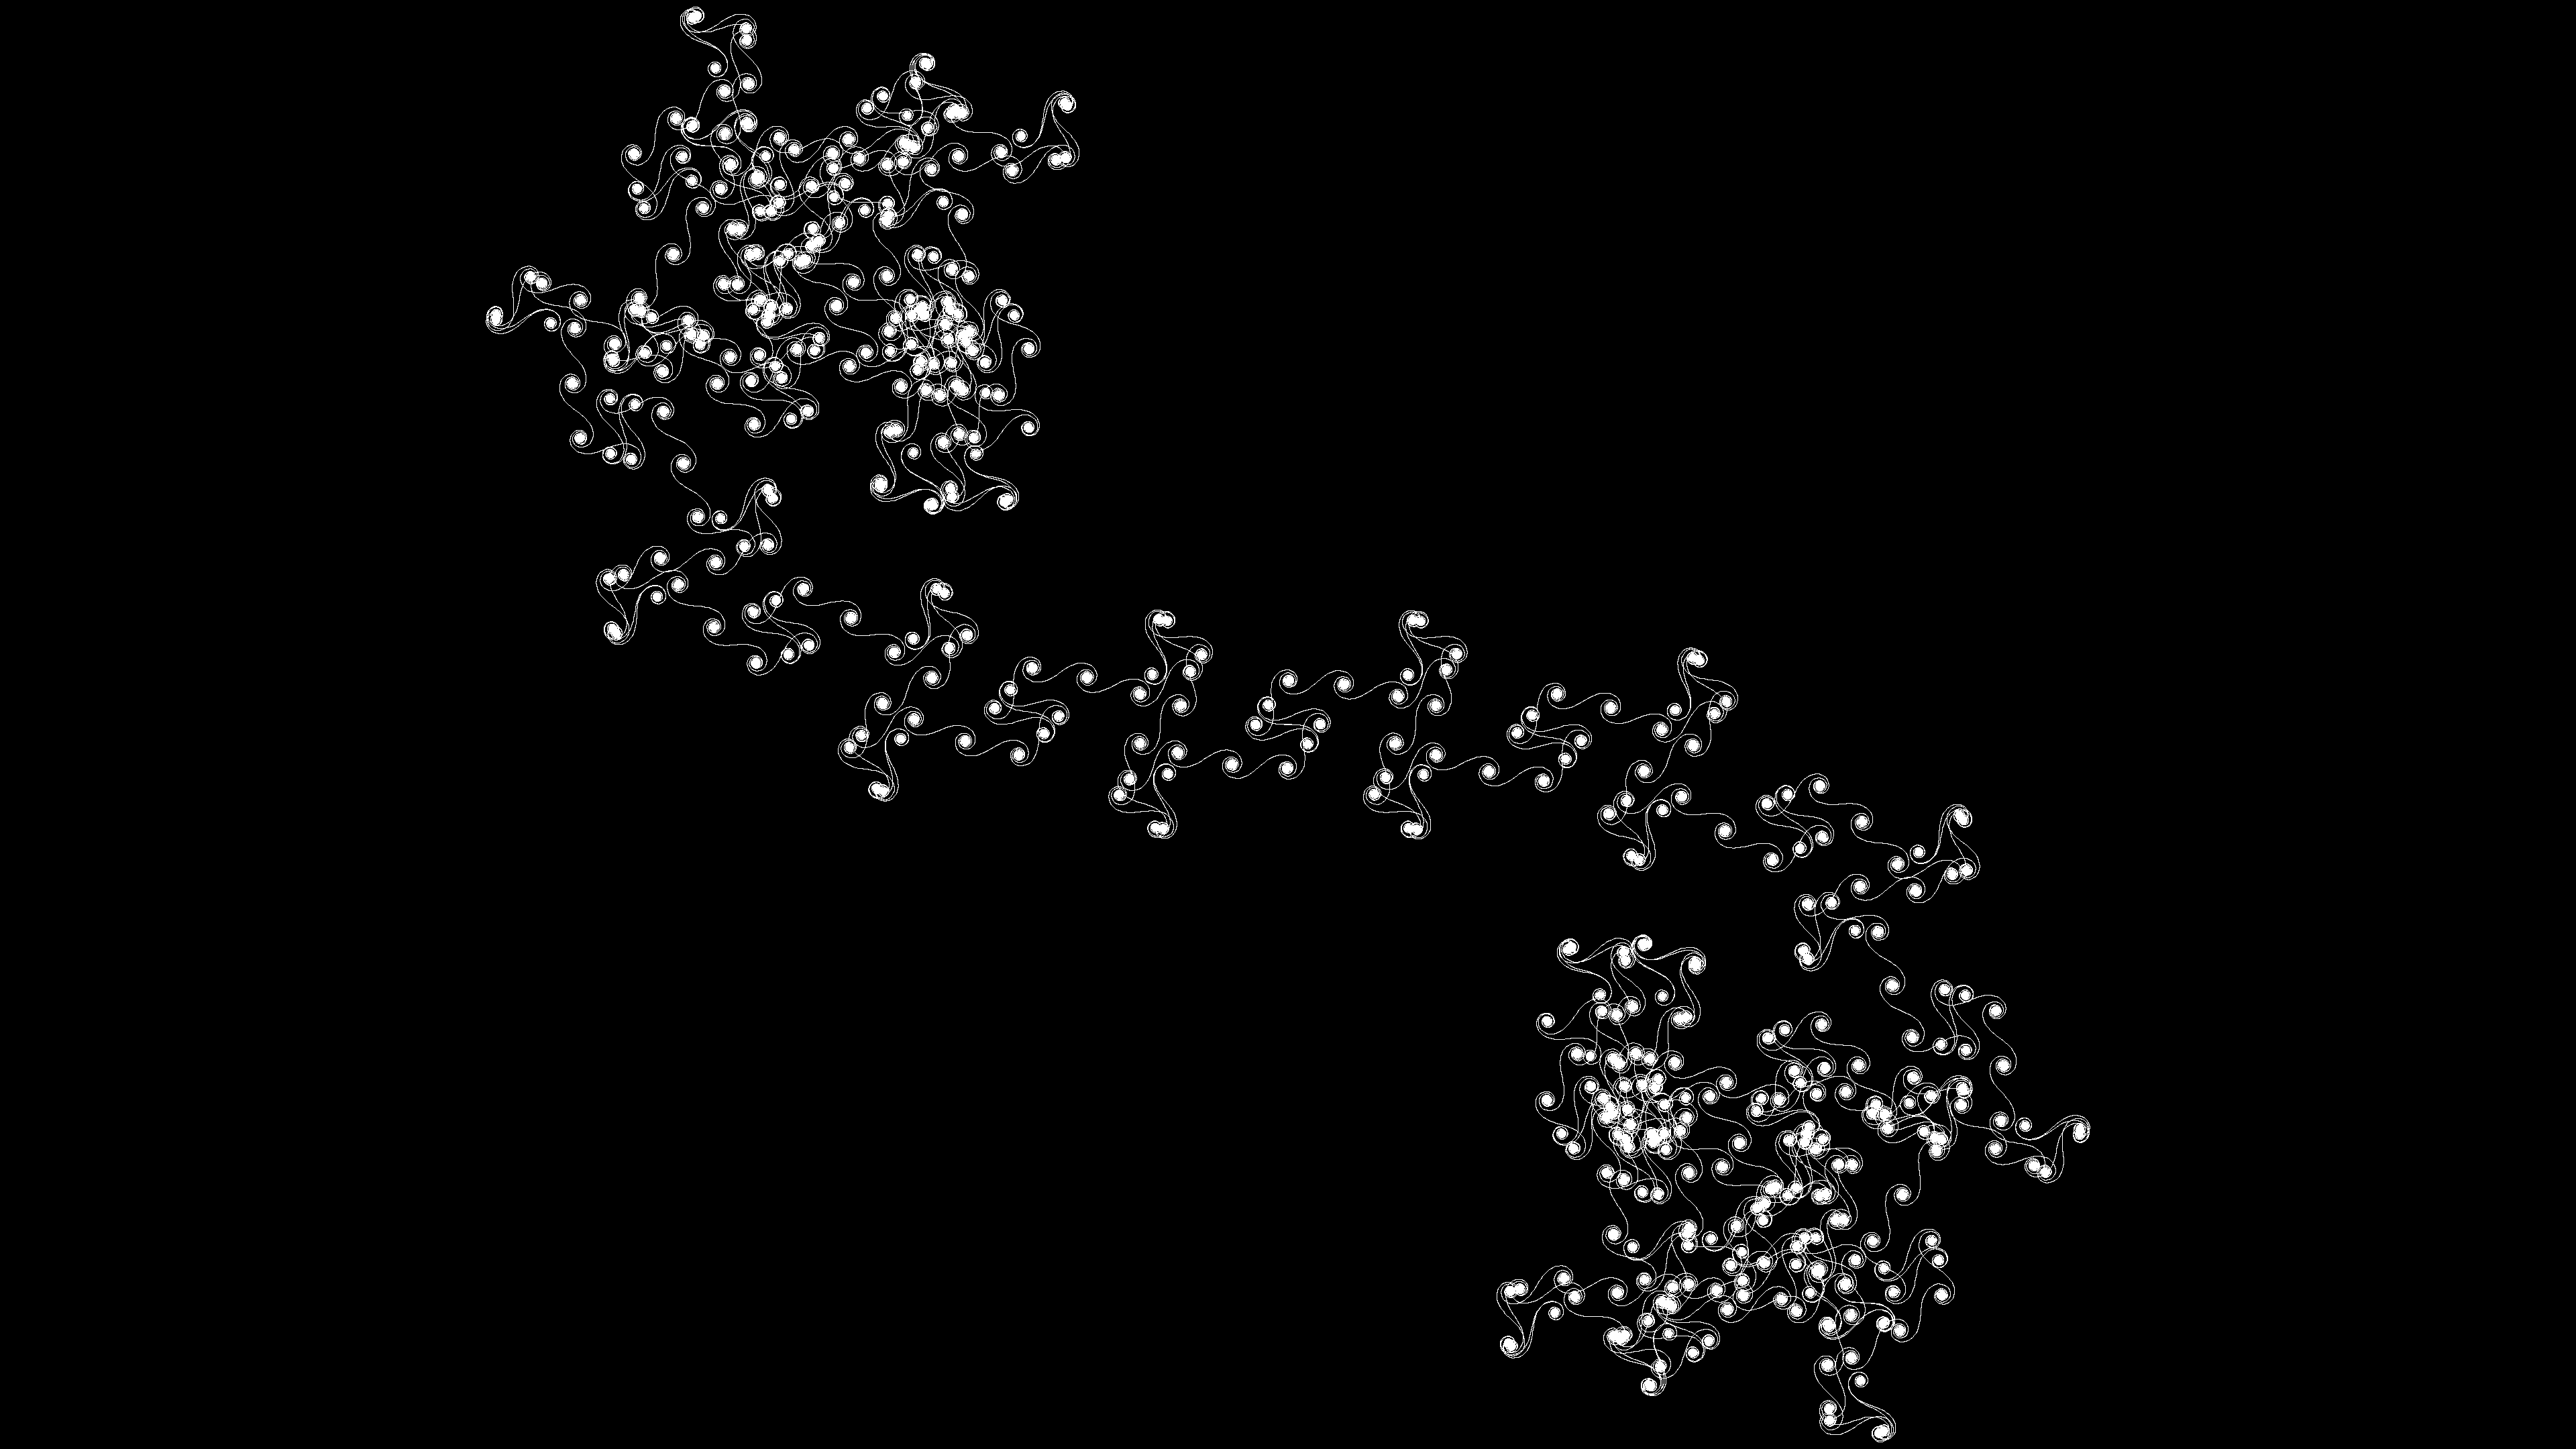
\includegraphics[width=\linewidth]{./stepsplusoneimages/0000000069.png}
    \caption{tf p=499 q=199668 theta=000 89969349.png}
  \end{subfigure}
  \begin{subfigure}[t]{0.48\textwidth}
    \centering
    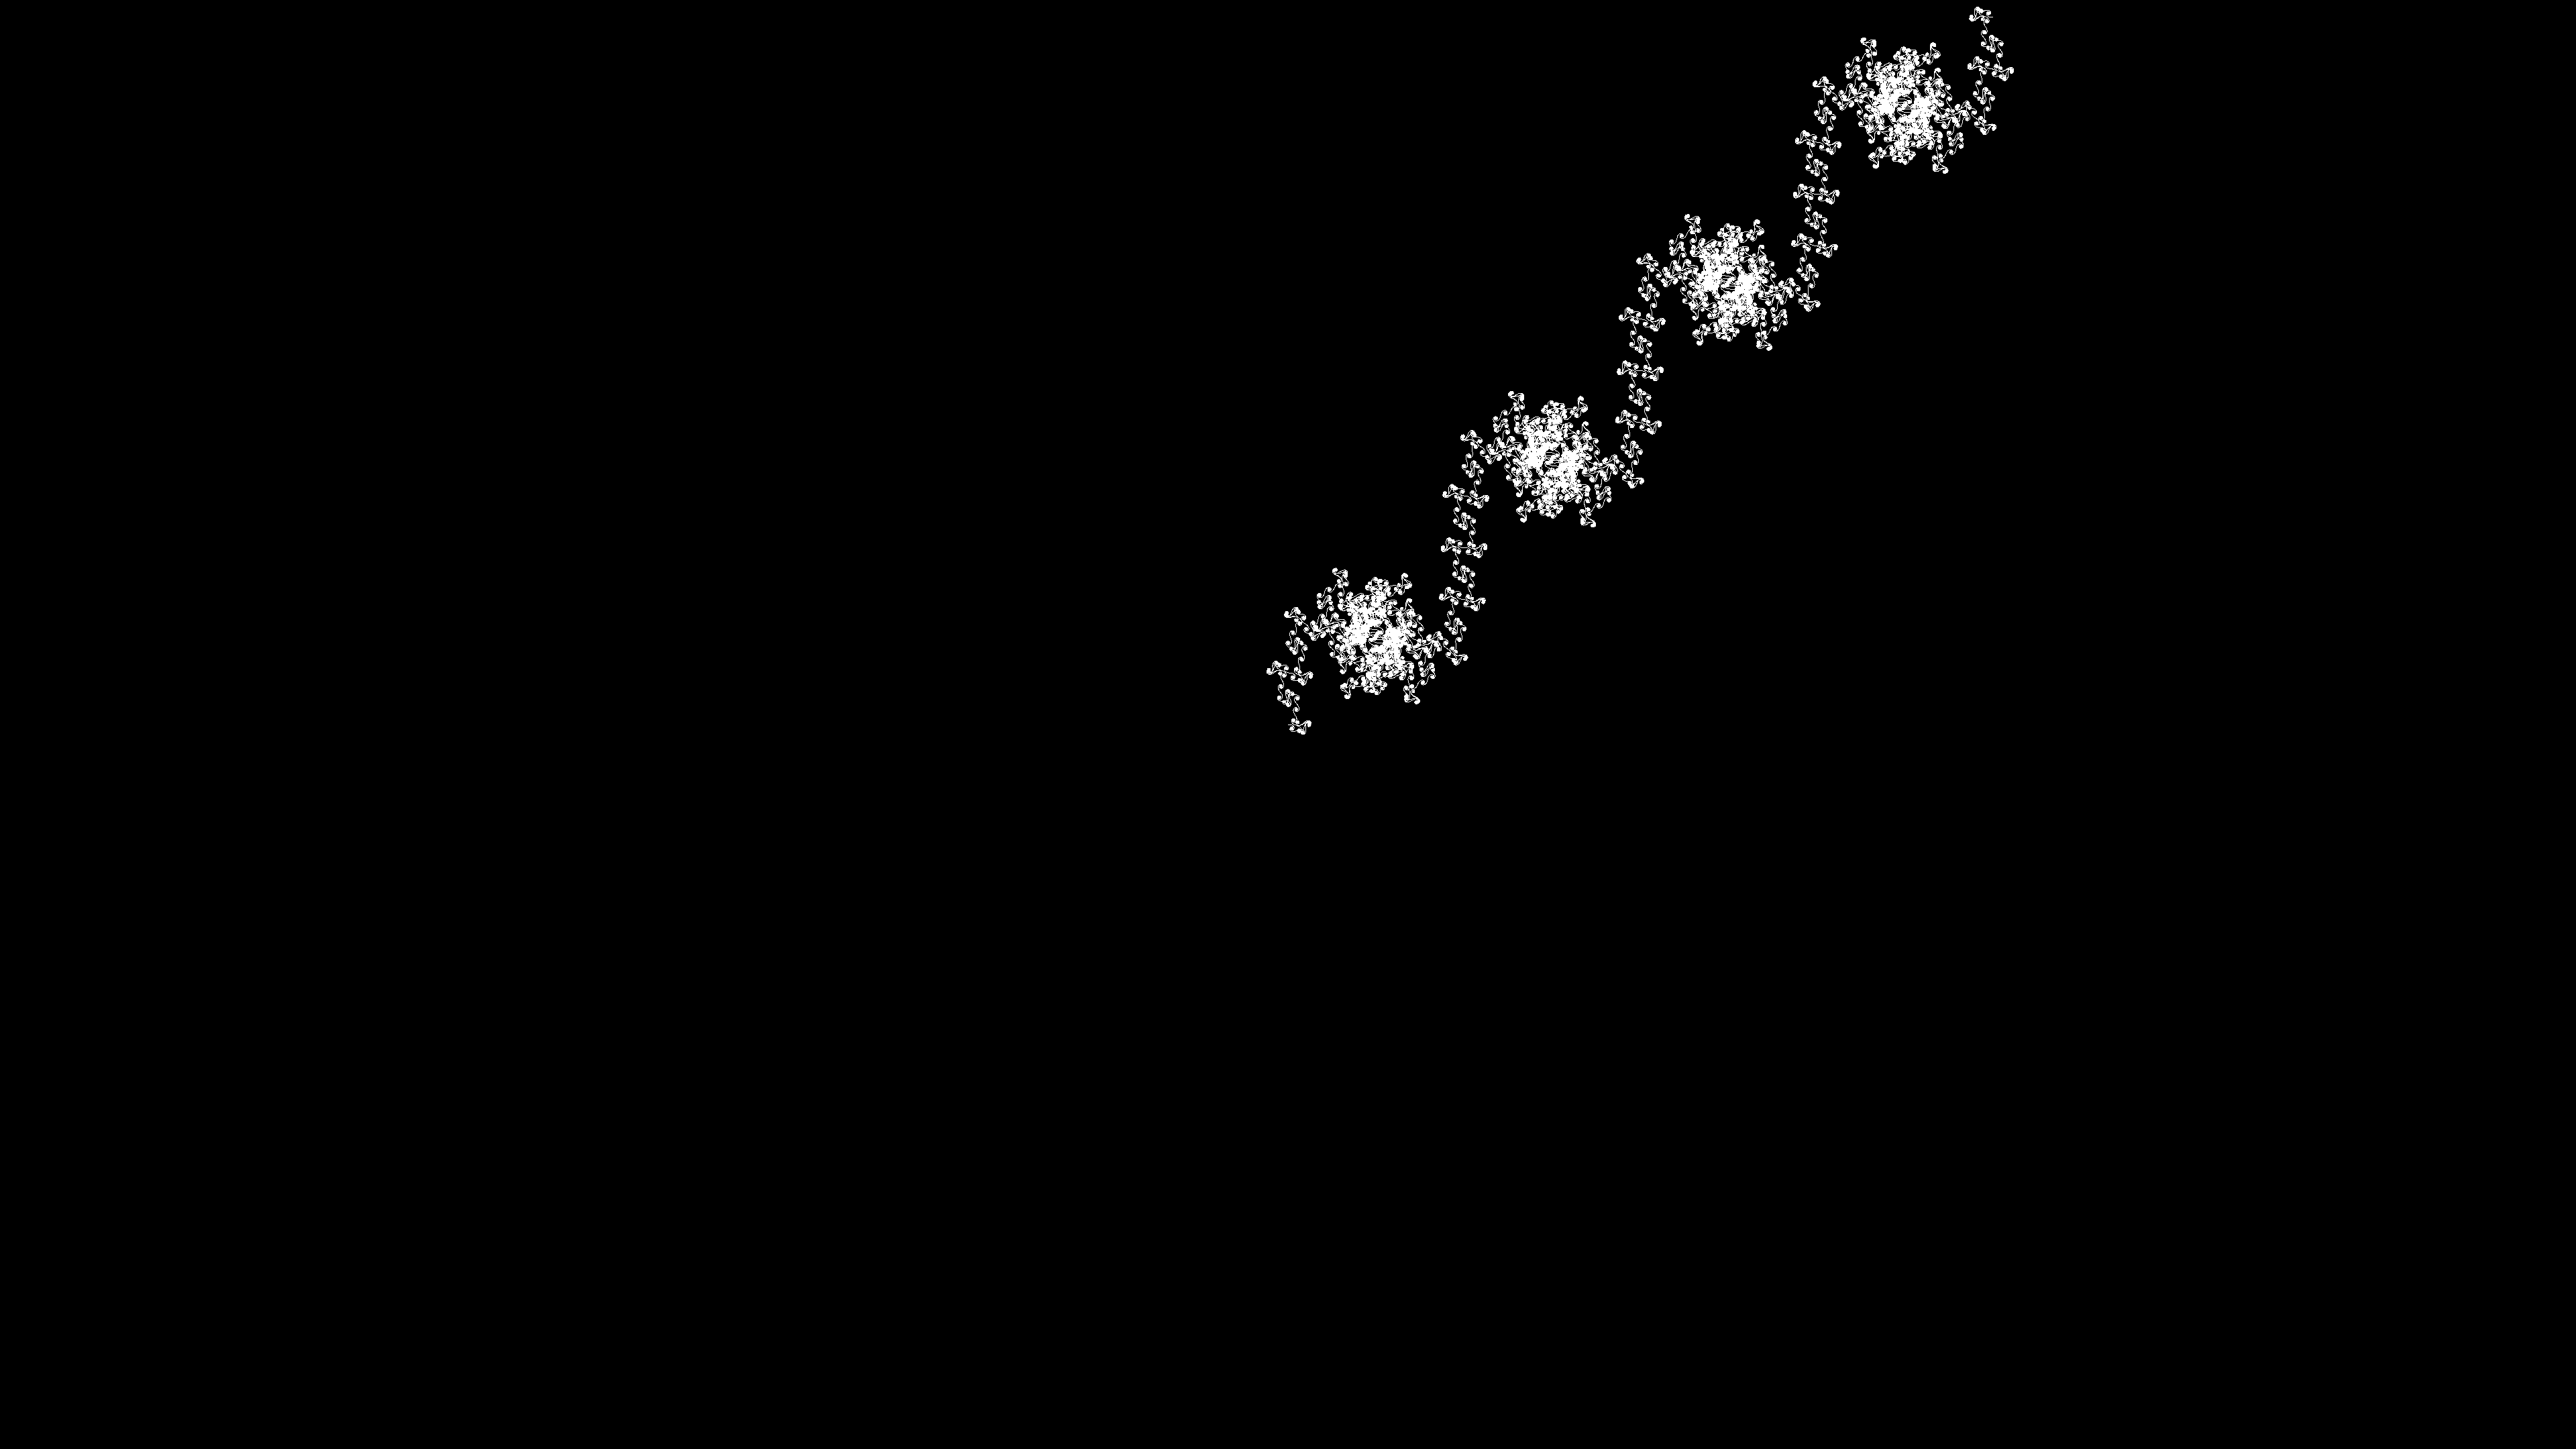
\includegraphics[width=\linewidth]{./stepsplusoneimages/0000000070.png}
    \caption{tf p=499 q=200167 theta=000 89745063.png}
  \end{subfigure}
  \caption{n=068 s=400 s+1=401}
  \label{fig:n=068}
\end{figure}
\begin{figure}[H]
  \centering
  \begin{subfigure}[t]{0.48\textwidth}
    \centering
    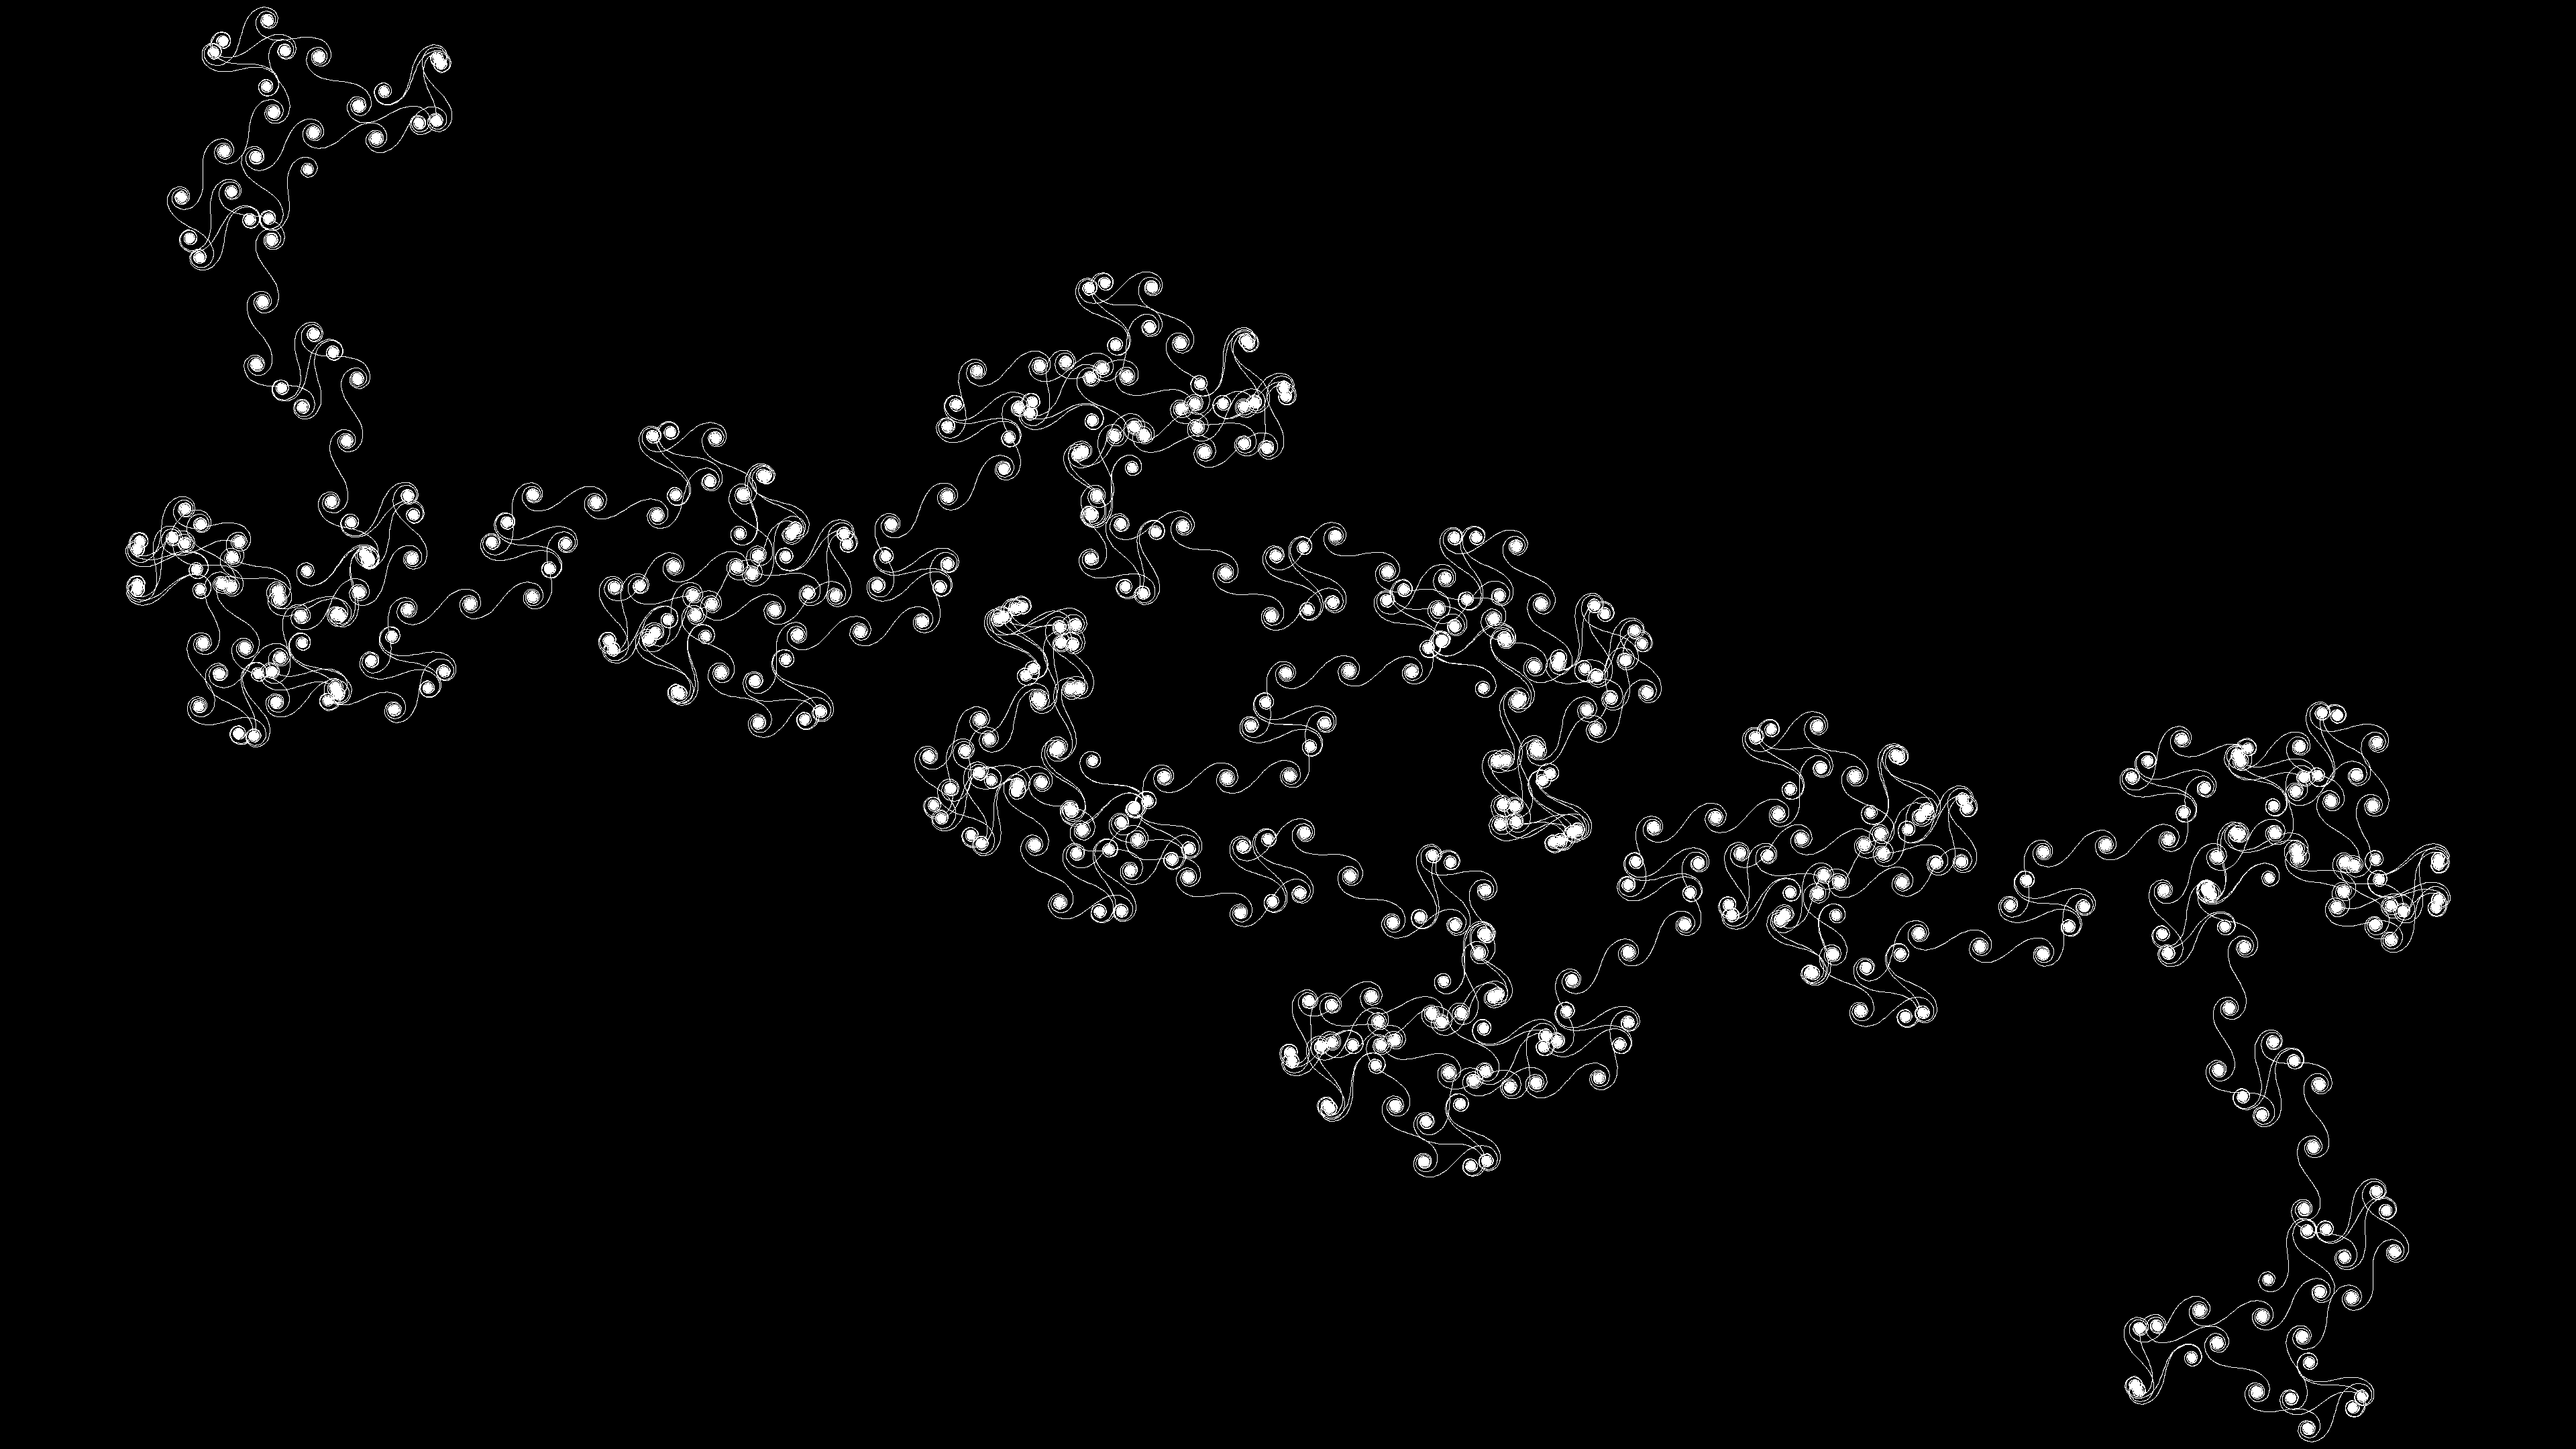
\includegraphics[width=\linewidth]{./stepsplusoneimages/0000000071.png}
    \caption{tf p=499 q=199670 theta=000 89968448.png}
  \end{subfigure}
  \begin{subfigure}[t]{0.48\textwidth}
    \centering
    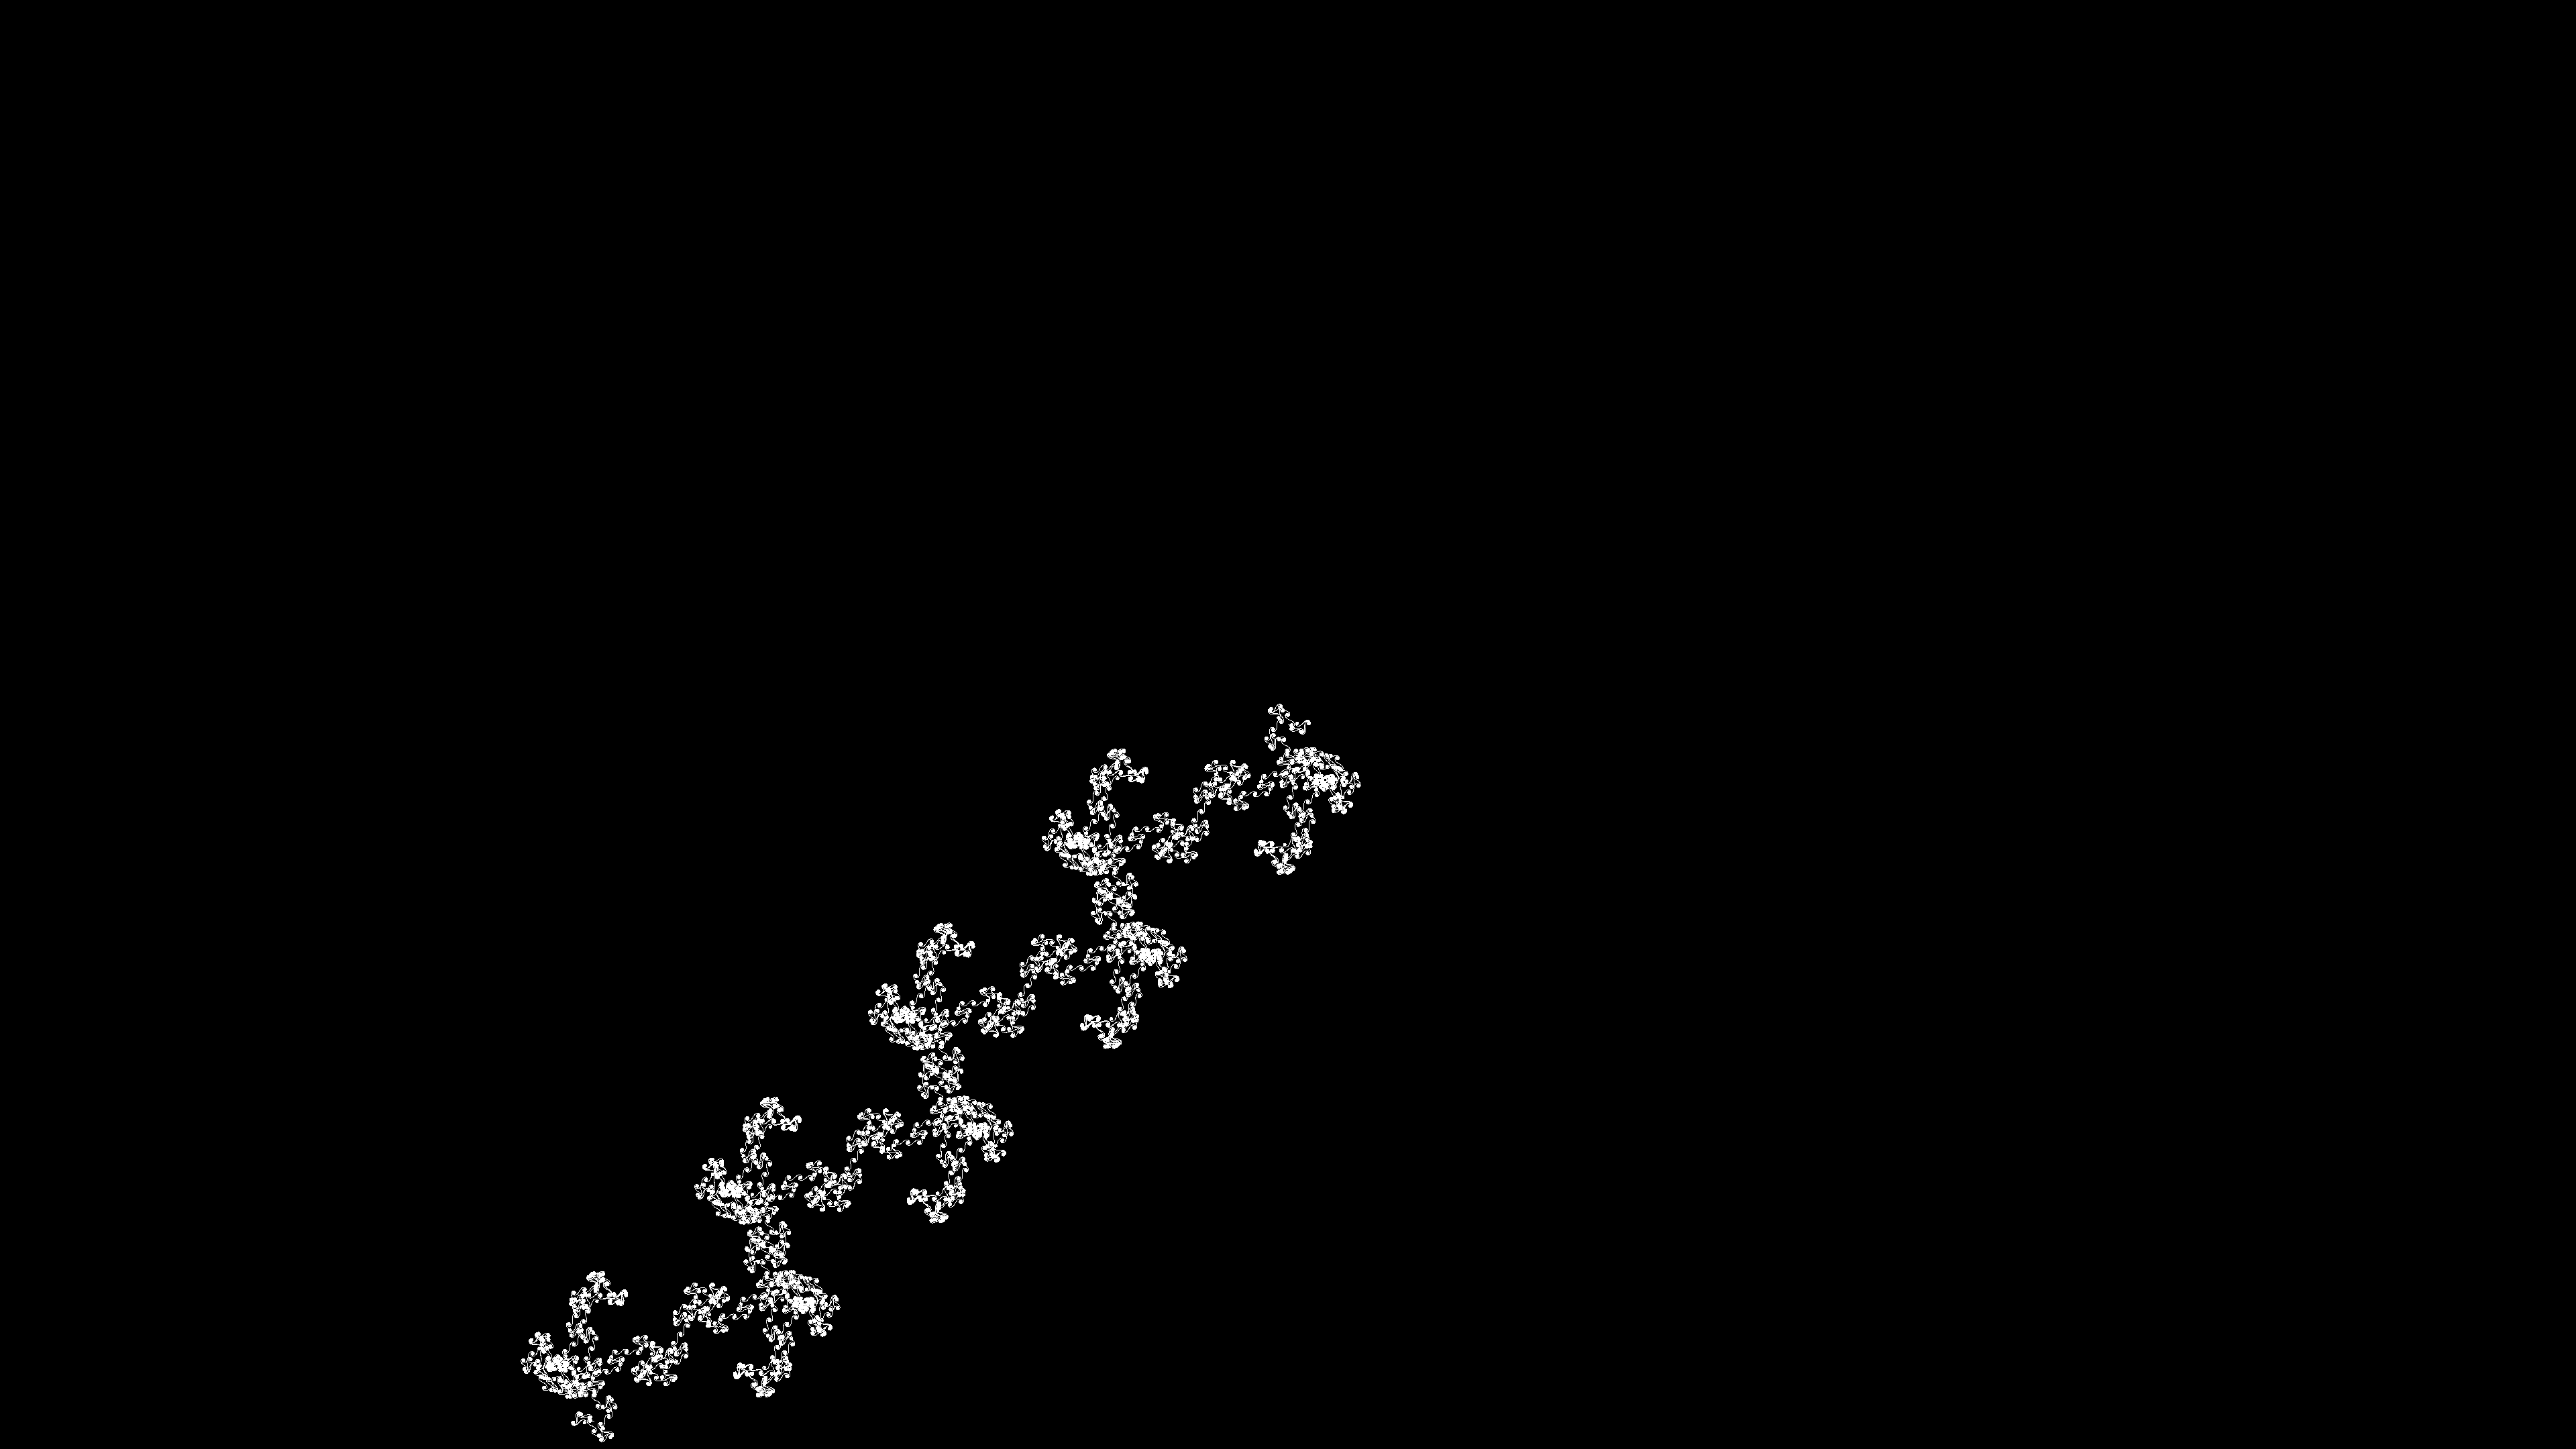
\includegraphics[width=\linewidth]{./stepsplusoneimages/0000000072.png}
    \caption{tf p=499 q=200169 theta=000 89744166.png}
  \end{subfigure}
  \caption{n=070 s=400 s+1=401}
  \label{fig:n=070}
\end{figure}
\begin{figure}[H]
  \centering
  \begin{subfigure}[t]{0.48\textwidth}
    \centering
    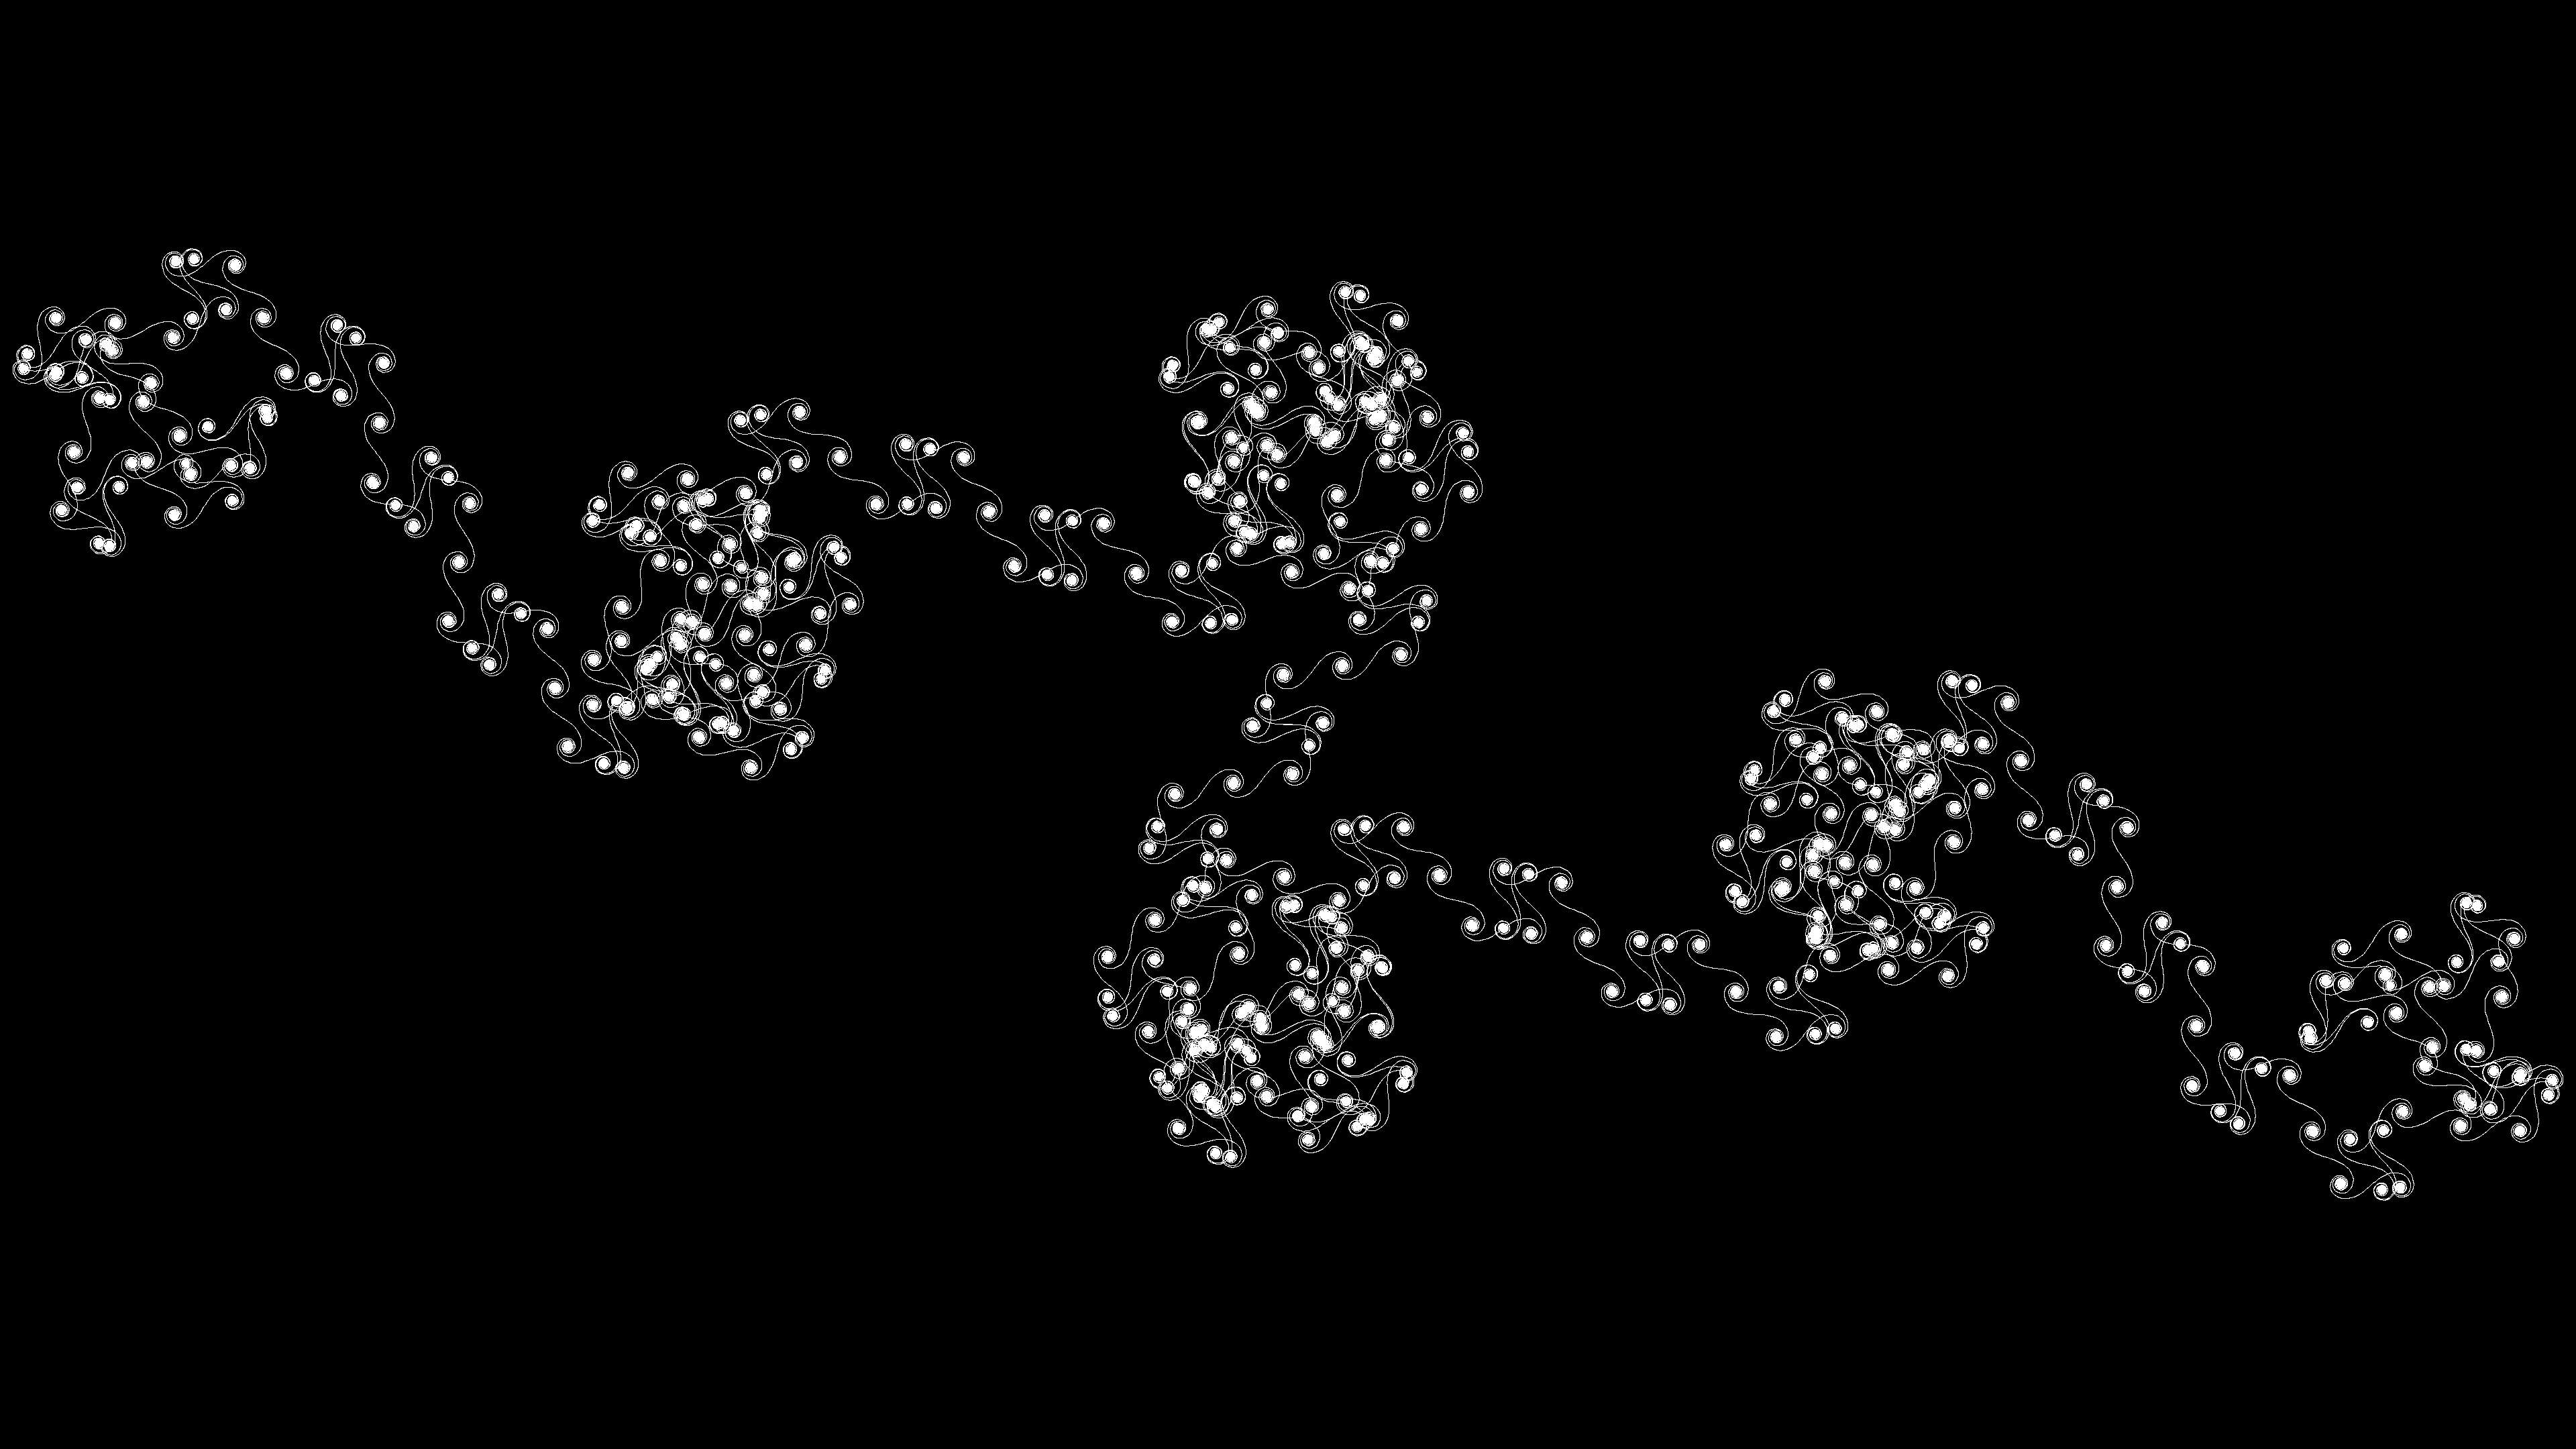
\includegraphics[width=\linewidth]{./stepsplusoneimages/0000000073.png}
    \caption{tf p=499 q=199672 theta=000 89967547.png}
  \end{subfigure}
  \begin{subfigure}[t]{0.48\textwidth}
    \centering
    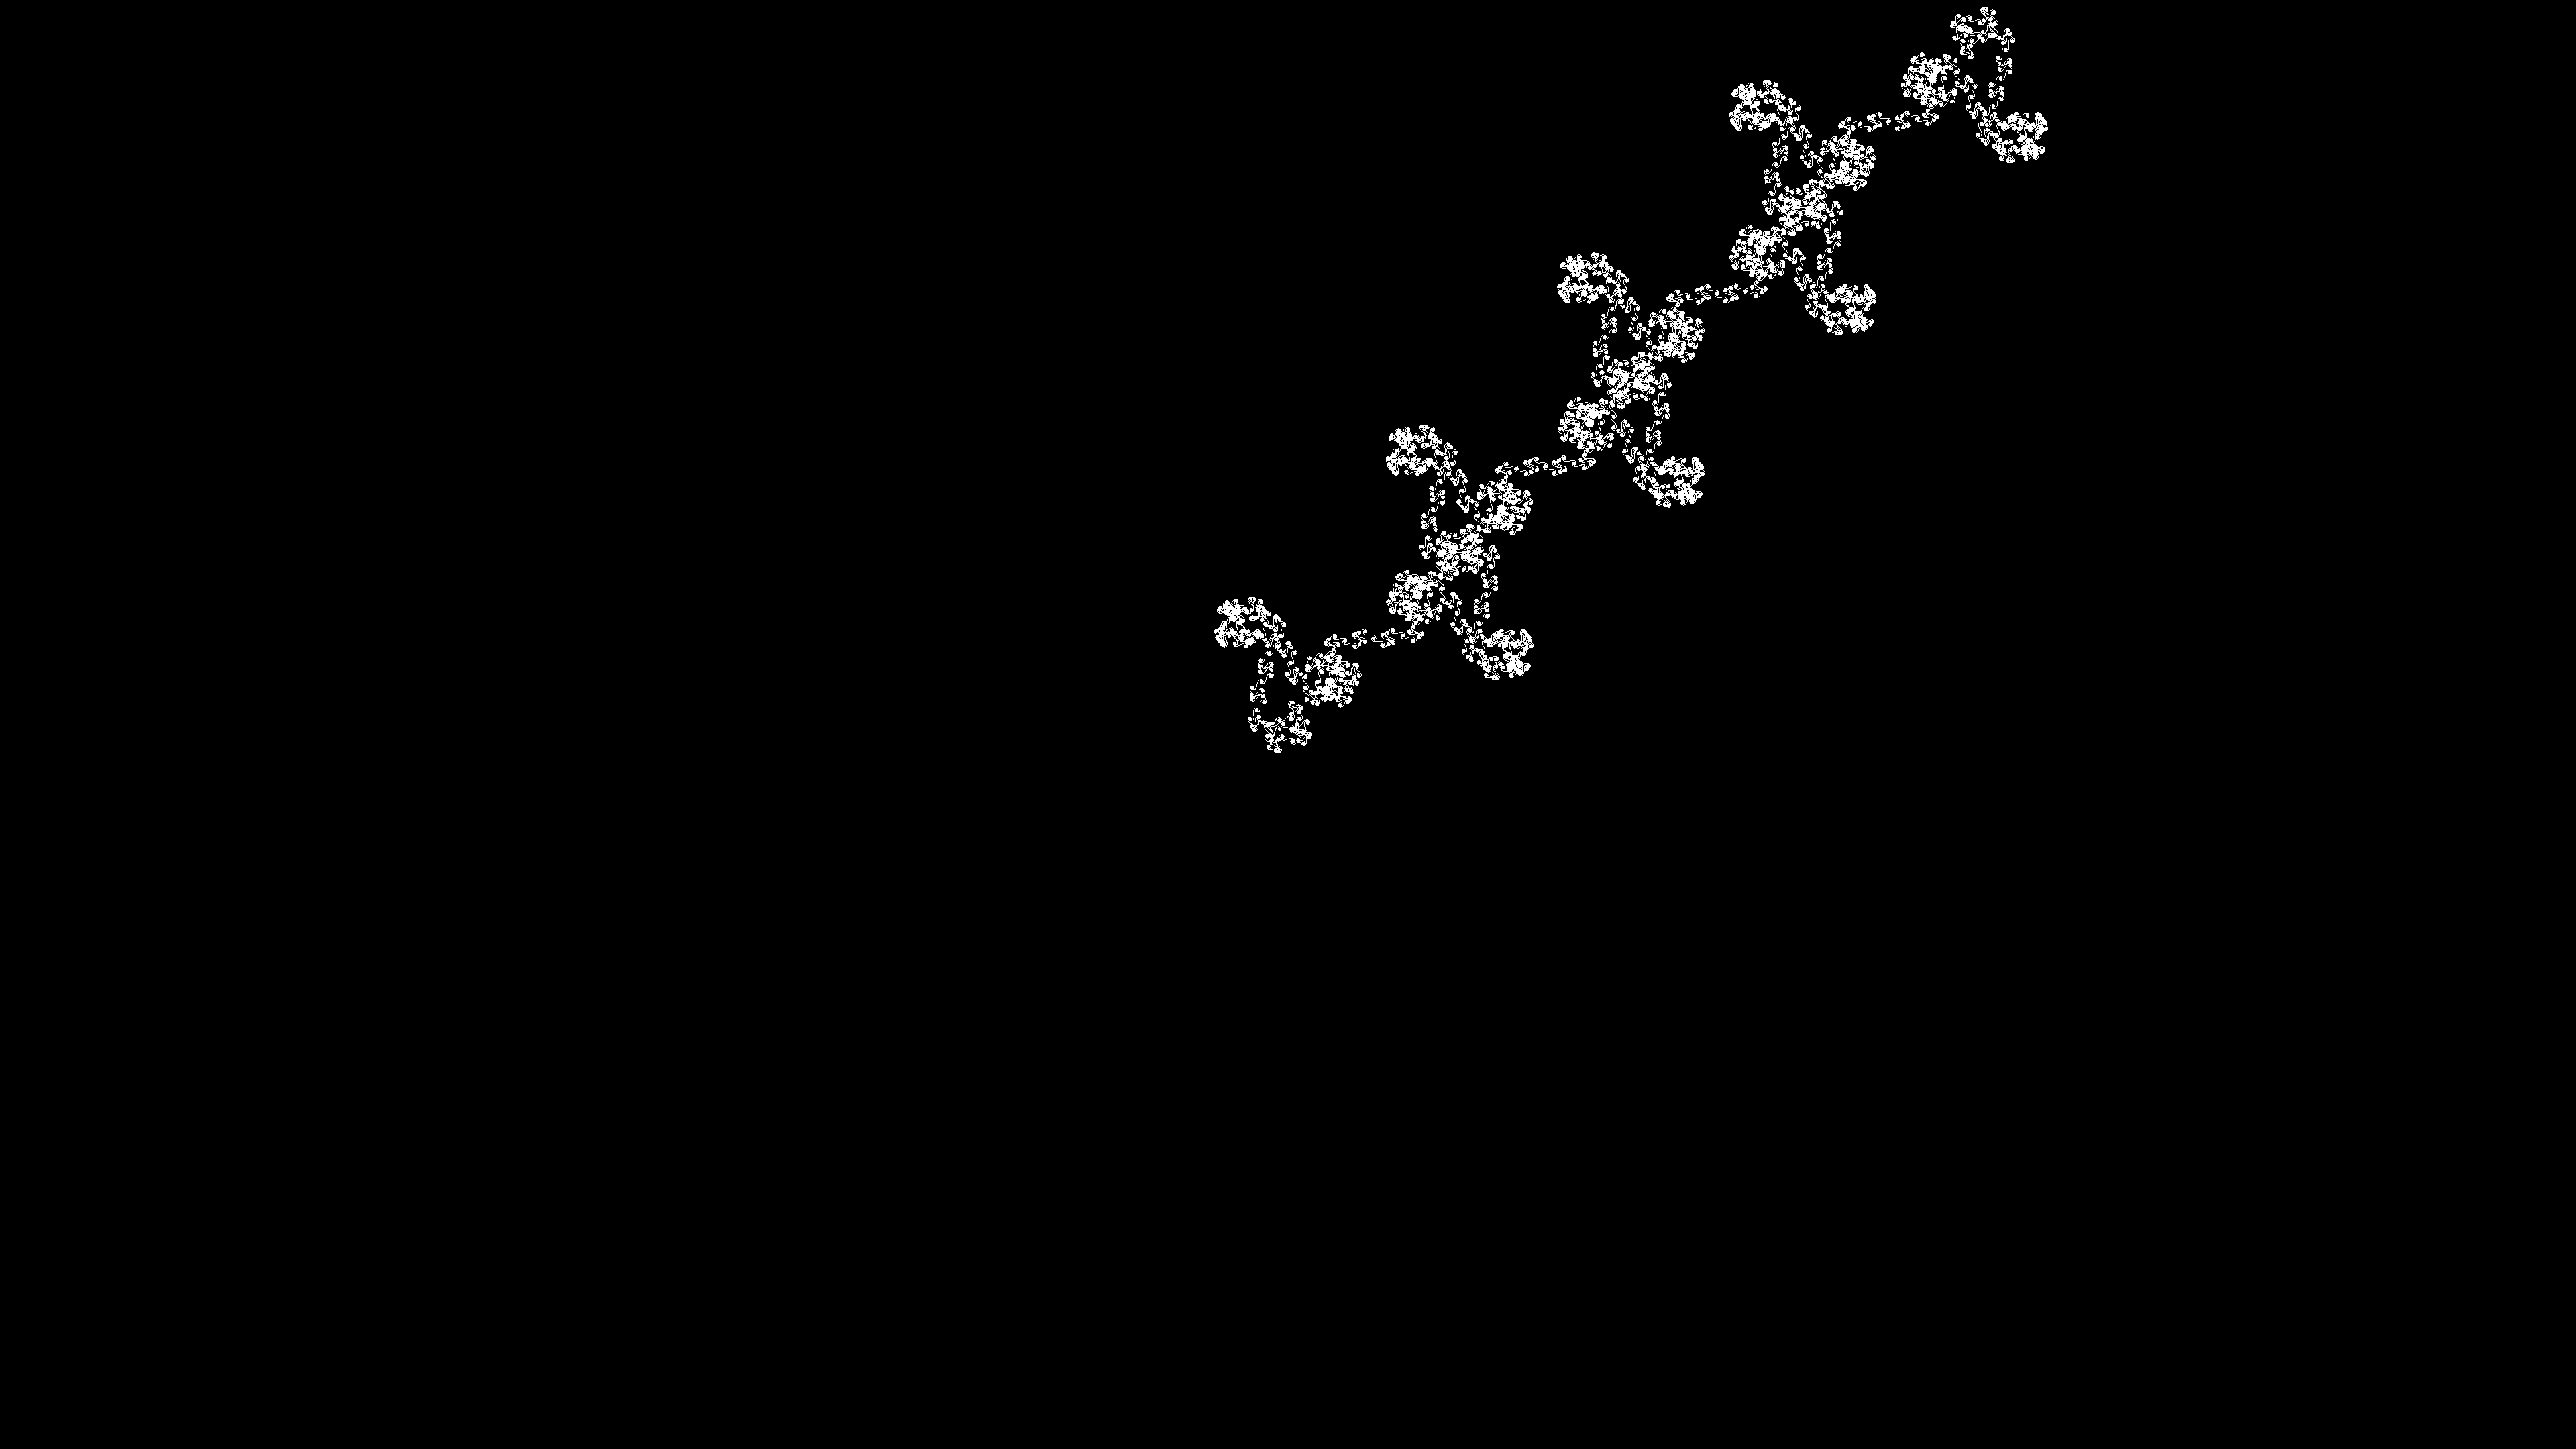
\includegraphics[width=\linewidth]{./stepsplusoneimages/0000000074.png}
    \caption{tf p=499 q=200171 theta=000 89743270.png}
  \end{subfigure}
  \caption{n=072 s=400 s+1=401}
  \label{fig:n=072}
\end{figure}
\begin{figure}[H]
  \centering
  \begin{subfigure}[t]{0.48\textwidth}
    \centering
    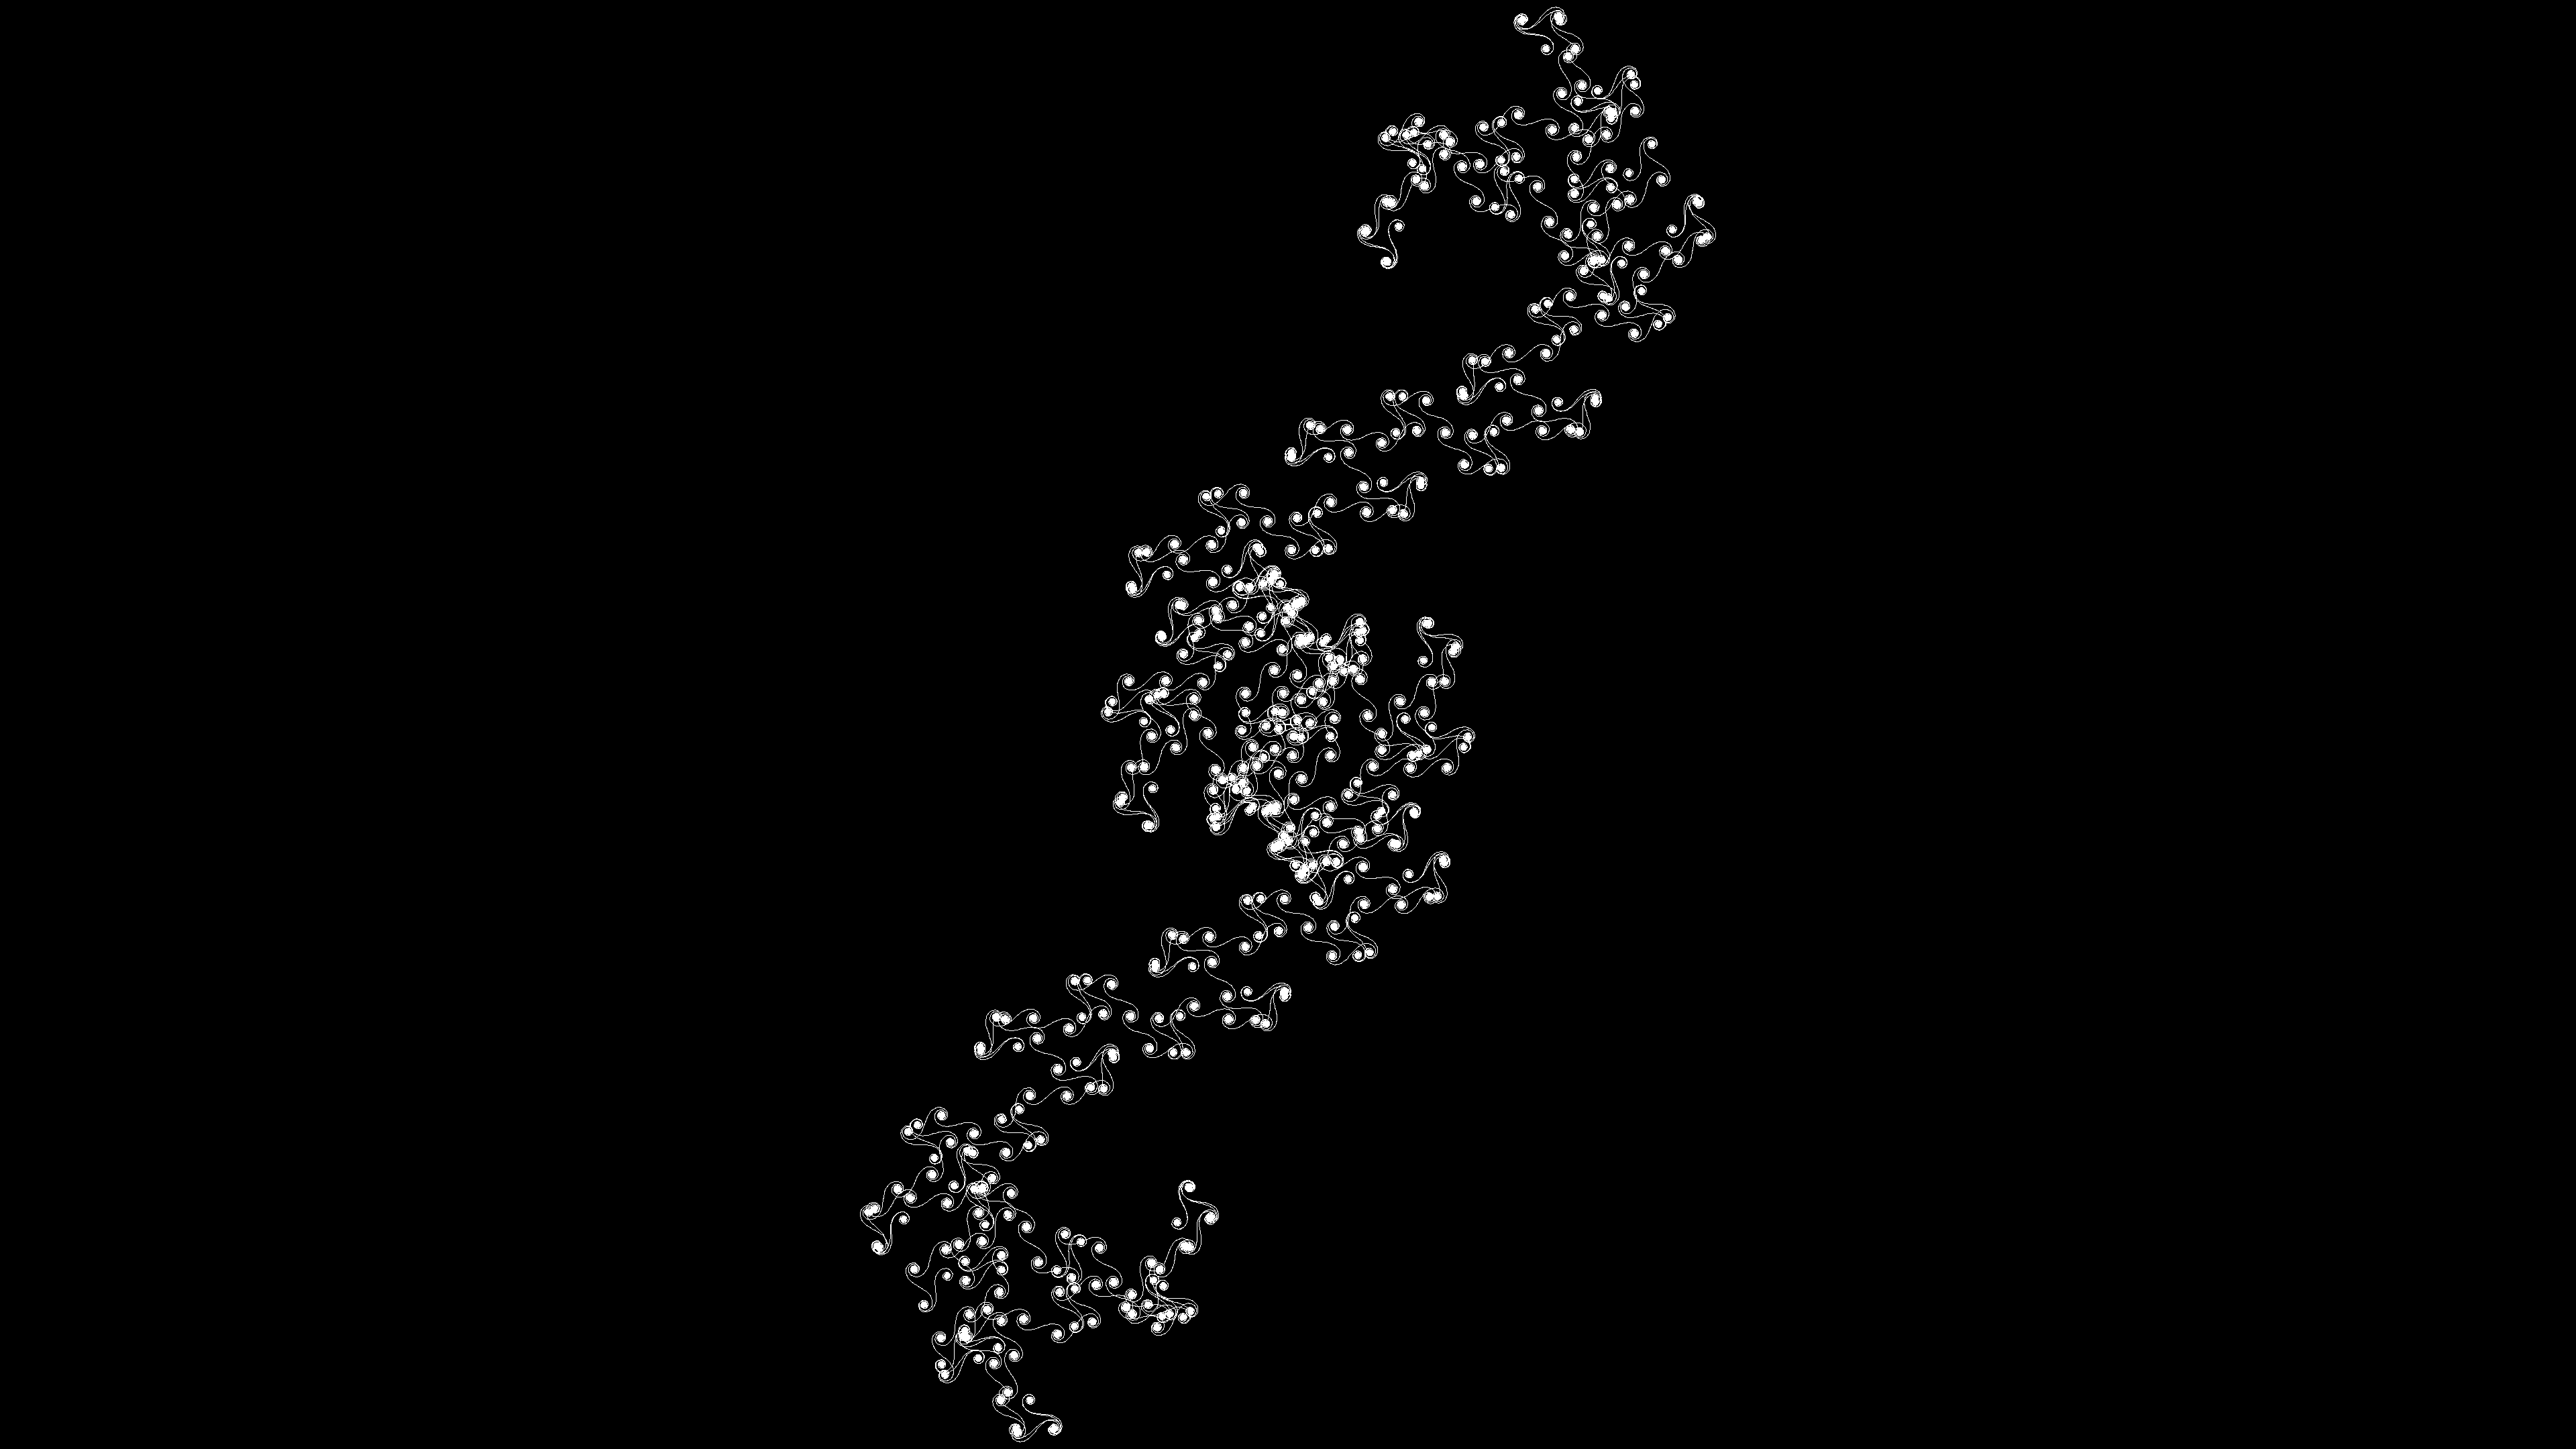
\includegraphics[width=\linewidth]{./stepsplusoneimages/0000000075.png}
    \caption{tf p=499 q=199674 theta=000 89966646.png}
  \end{subfigure}
  \begin{subfigure}[t]{0.48\textwidth}
    \centering
    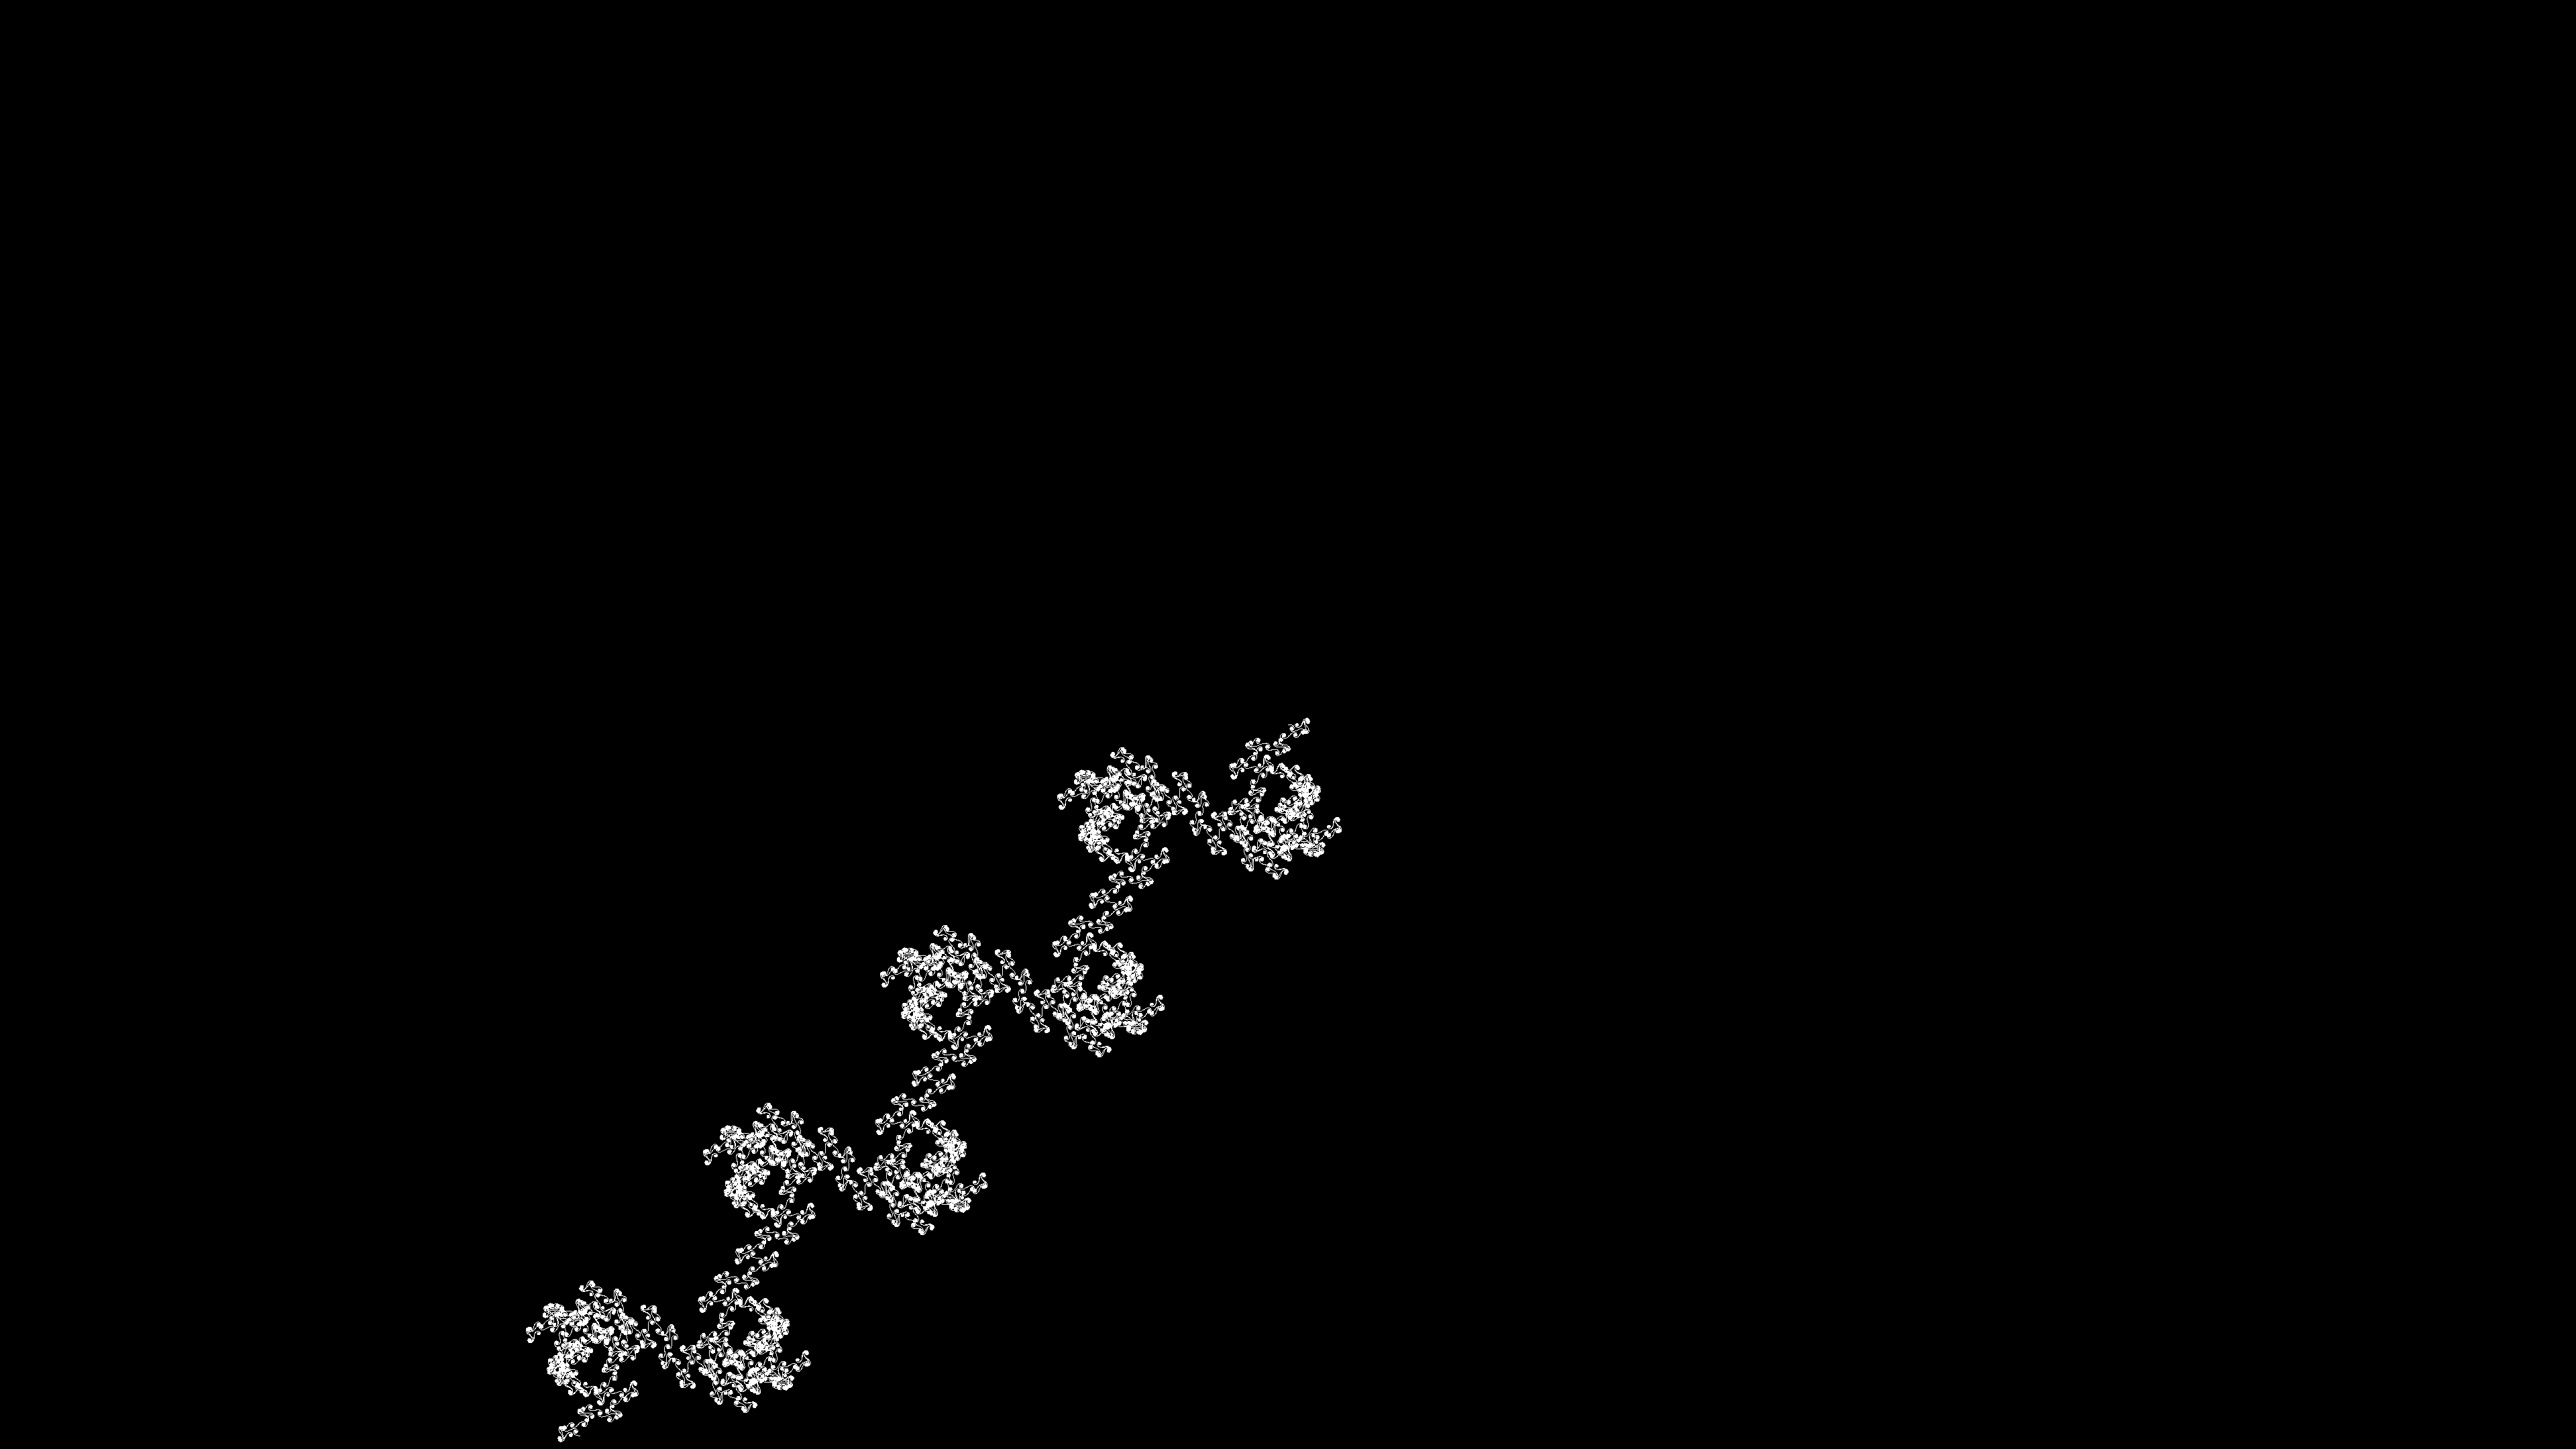
\includegraphics[width=\linewidth]{./stepsplusoneimages/0000000076.png}
    \caption{tf p=499 q=200173 theta=000 89742373.png}
  \end{subfigure}
  \caption{n=074 s=400 s+1=401}
  \label{fig:n=074}
\end{figure}
\begin{figure}[H]
  \centering
  \begin{subfigure}[t]{0.48\textwidth}
    \centering
    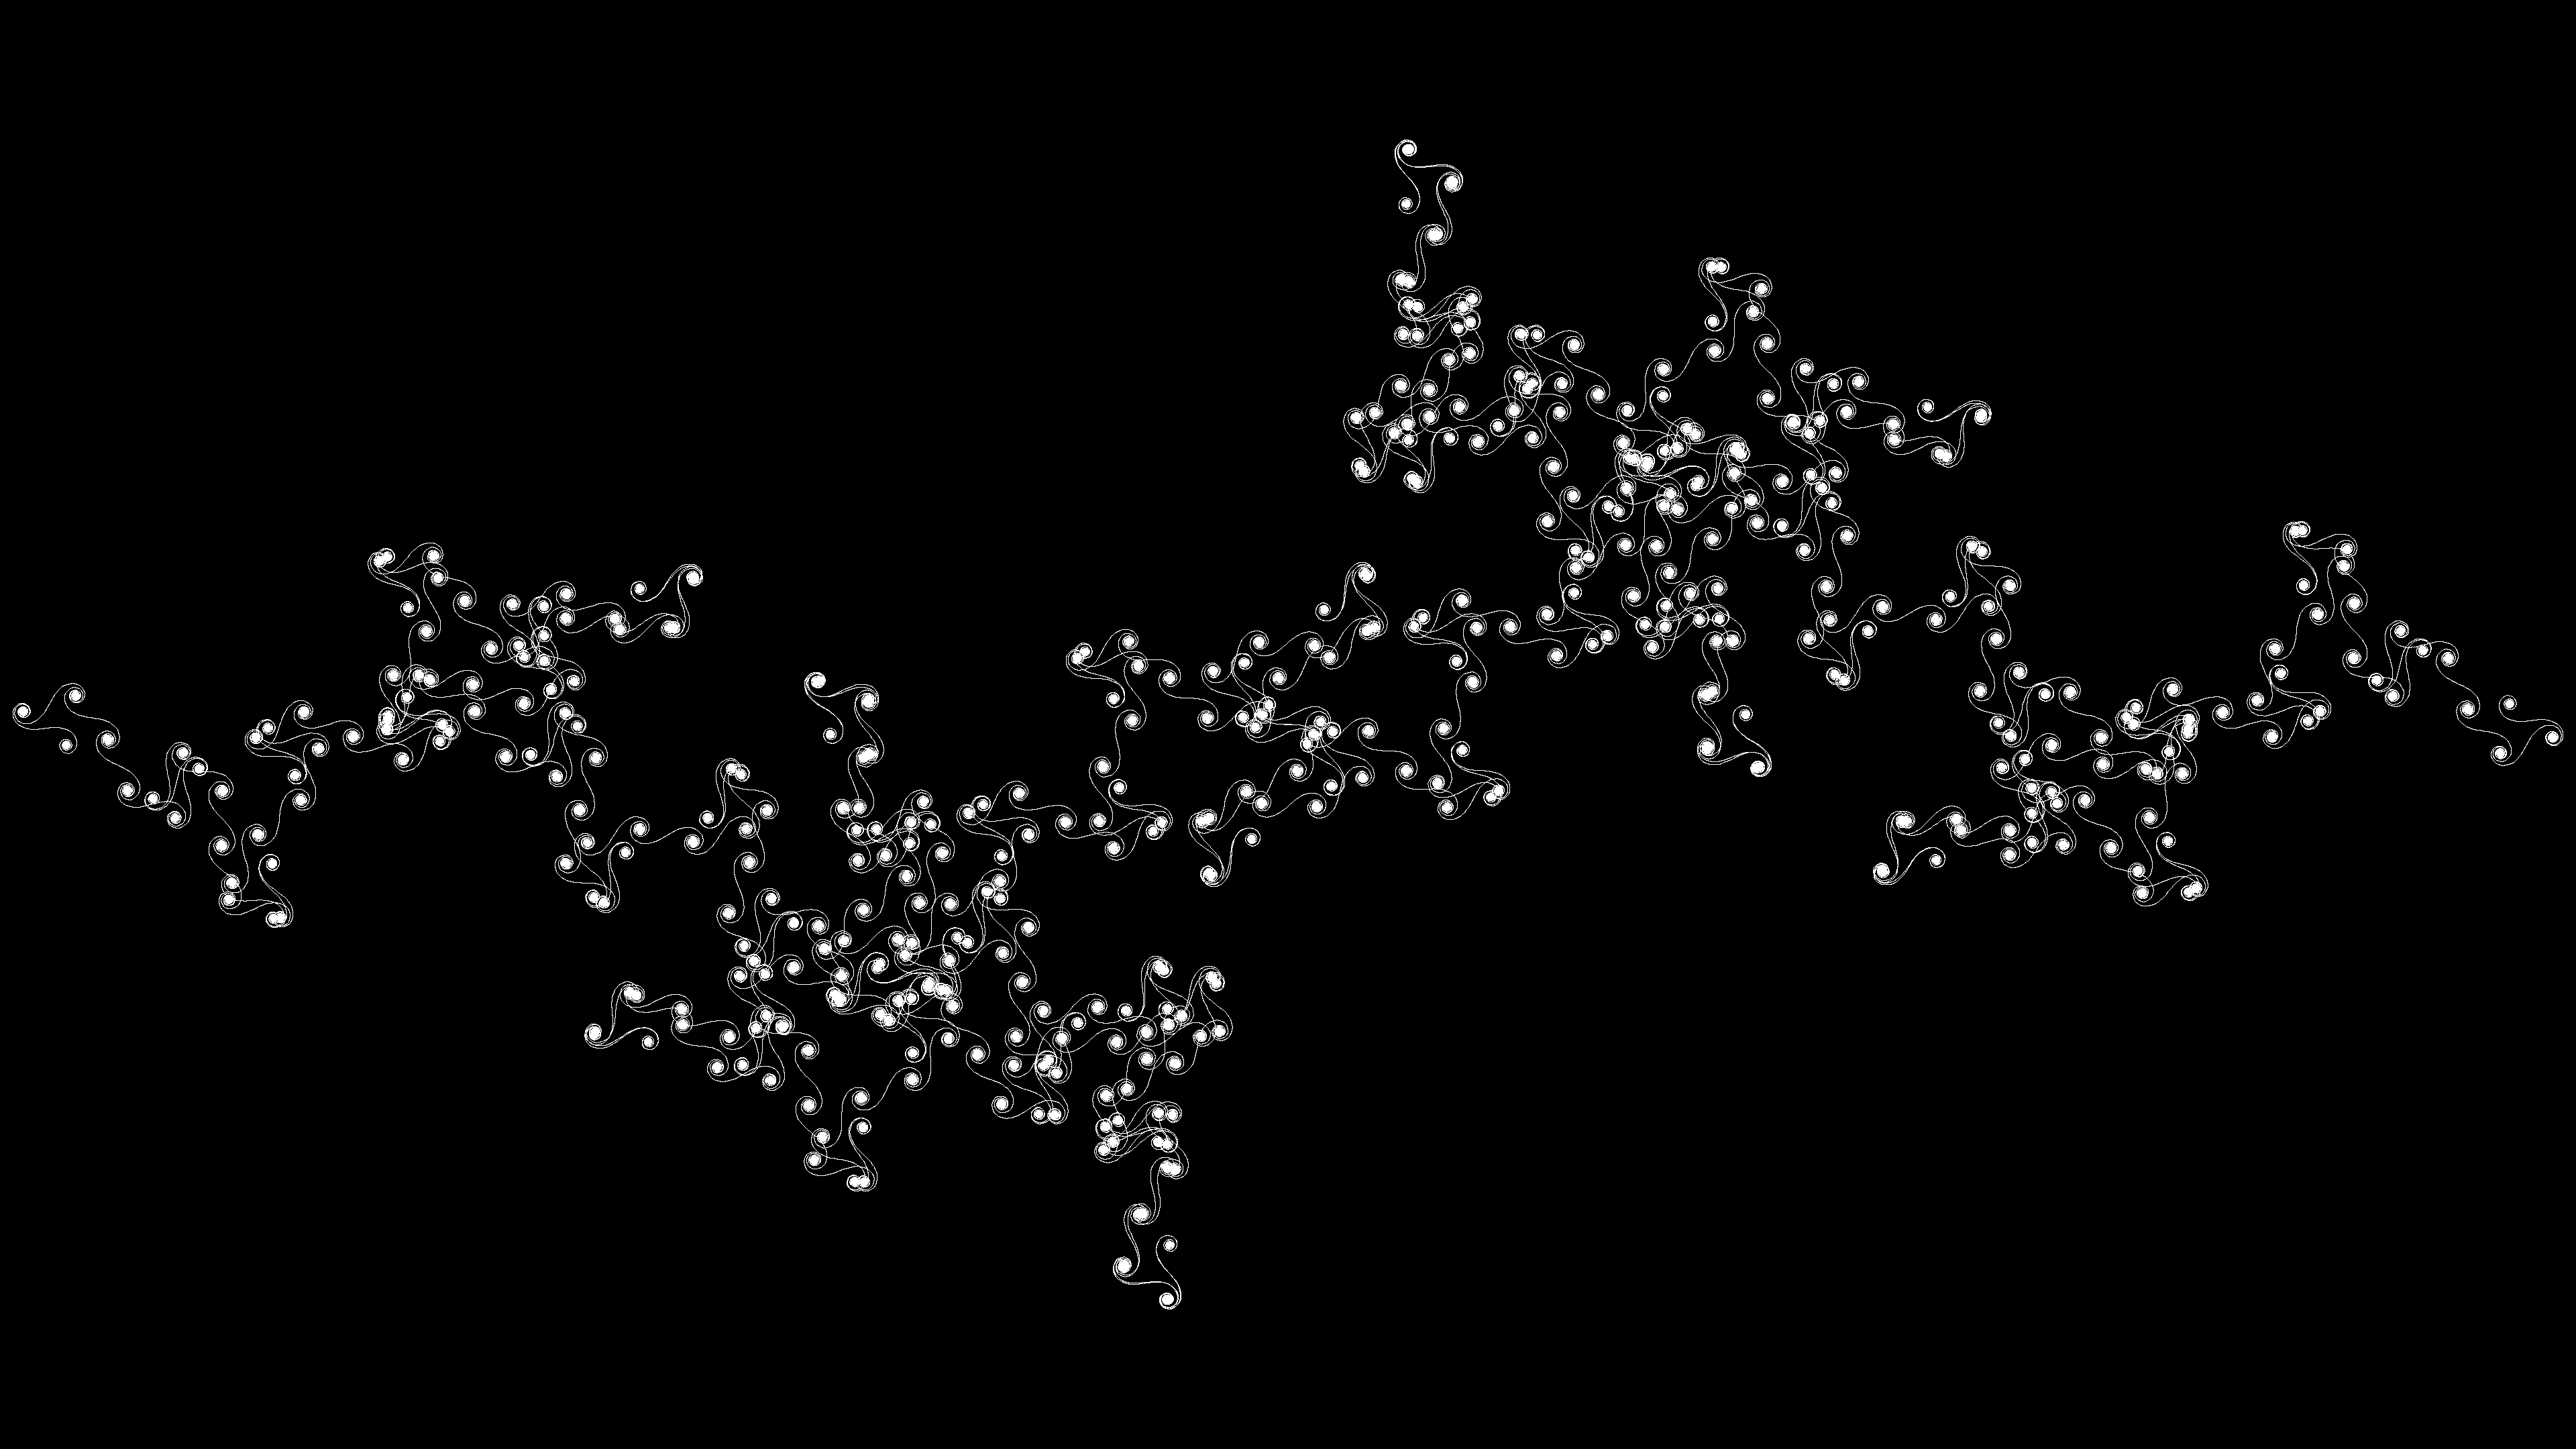
\includegraphics[width=\linewidth]{./stepsplusoneimages/0000000077.png}
    \caption{tf p=499 q=199676 theta=000 89965745.png}
  \end{subfigure}
  \begin{subfigure}[t]{0.48\textwidth}
    \centering
    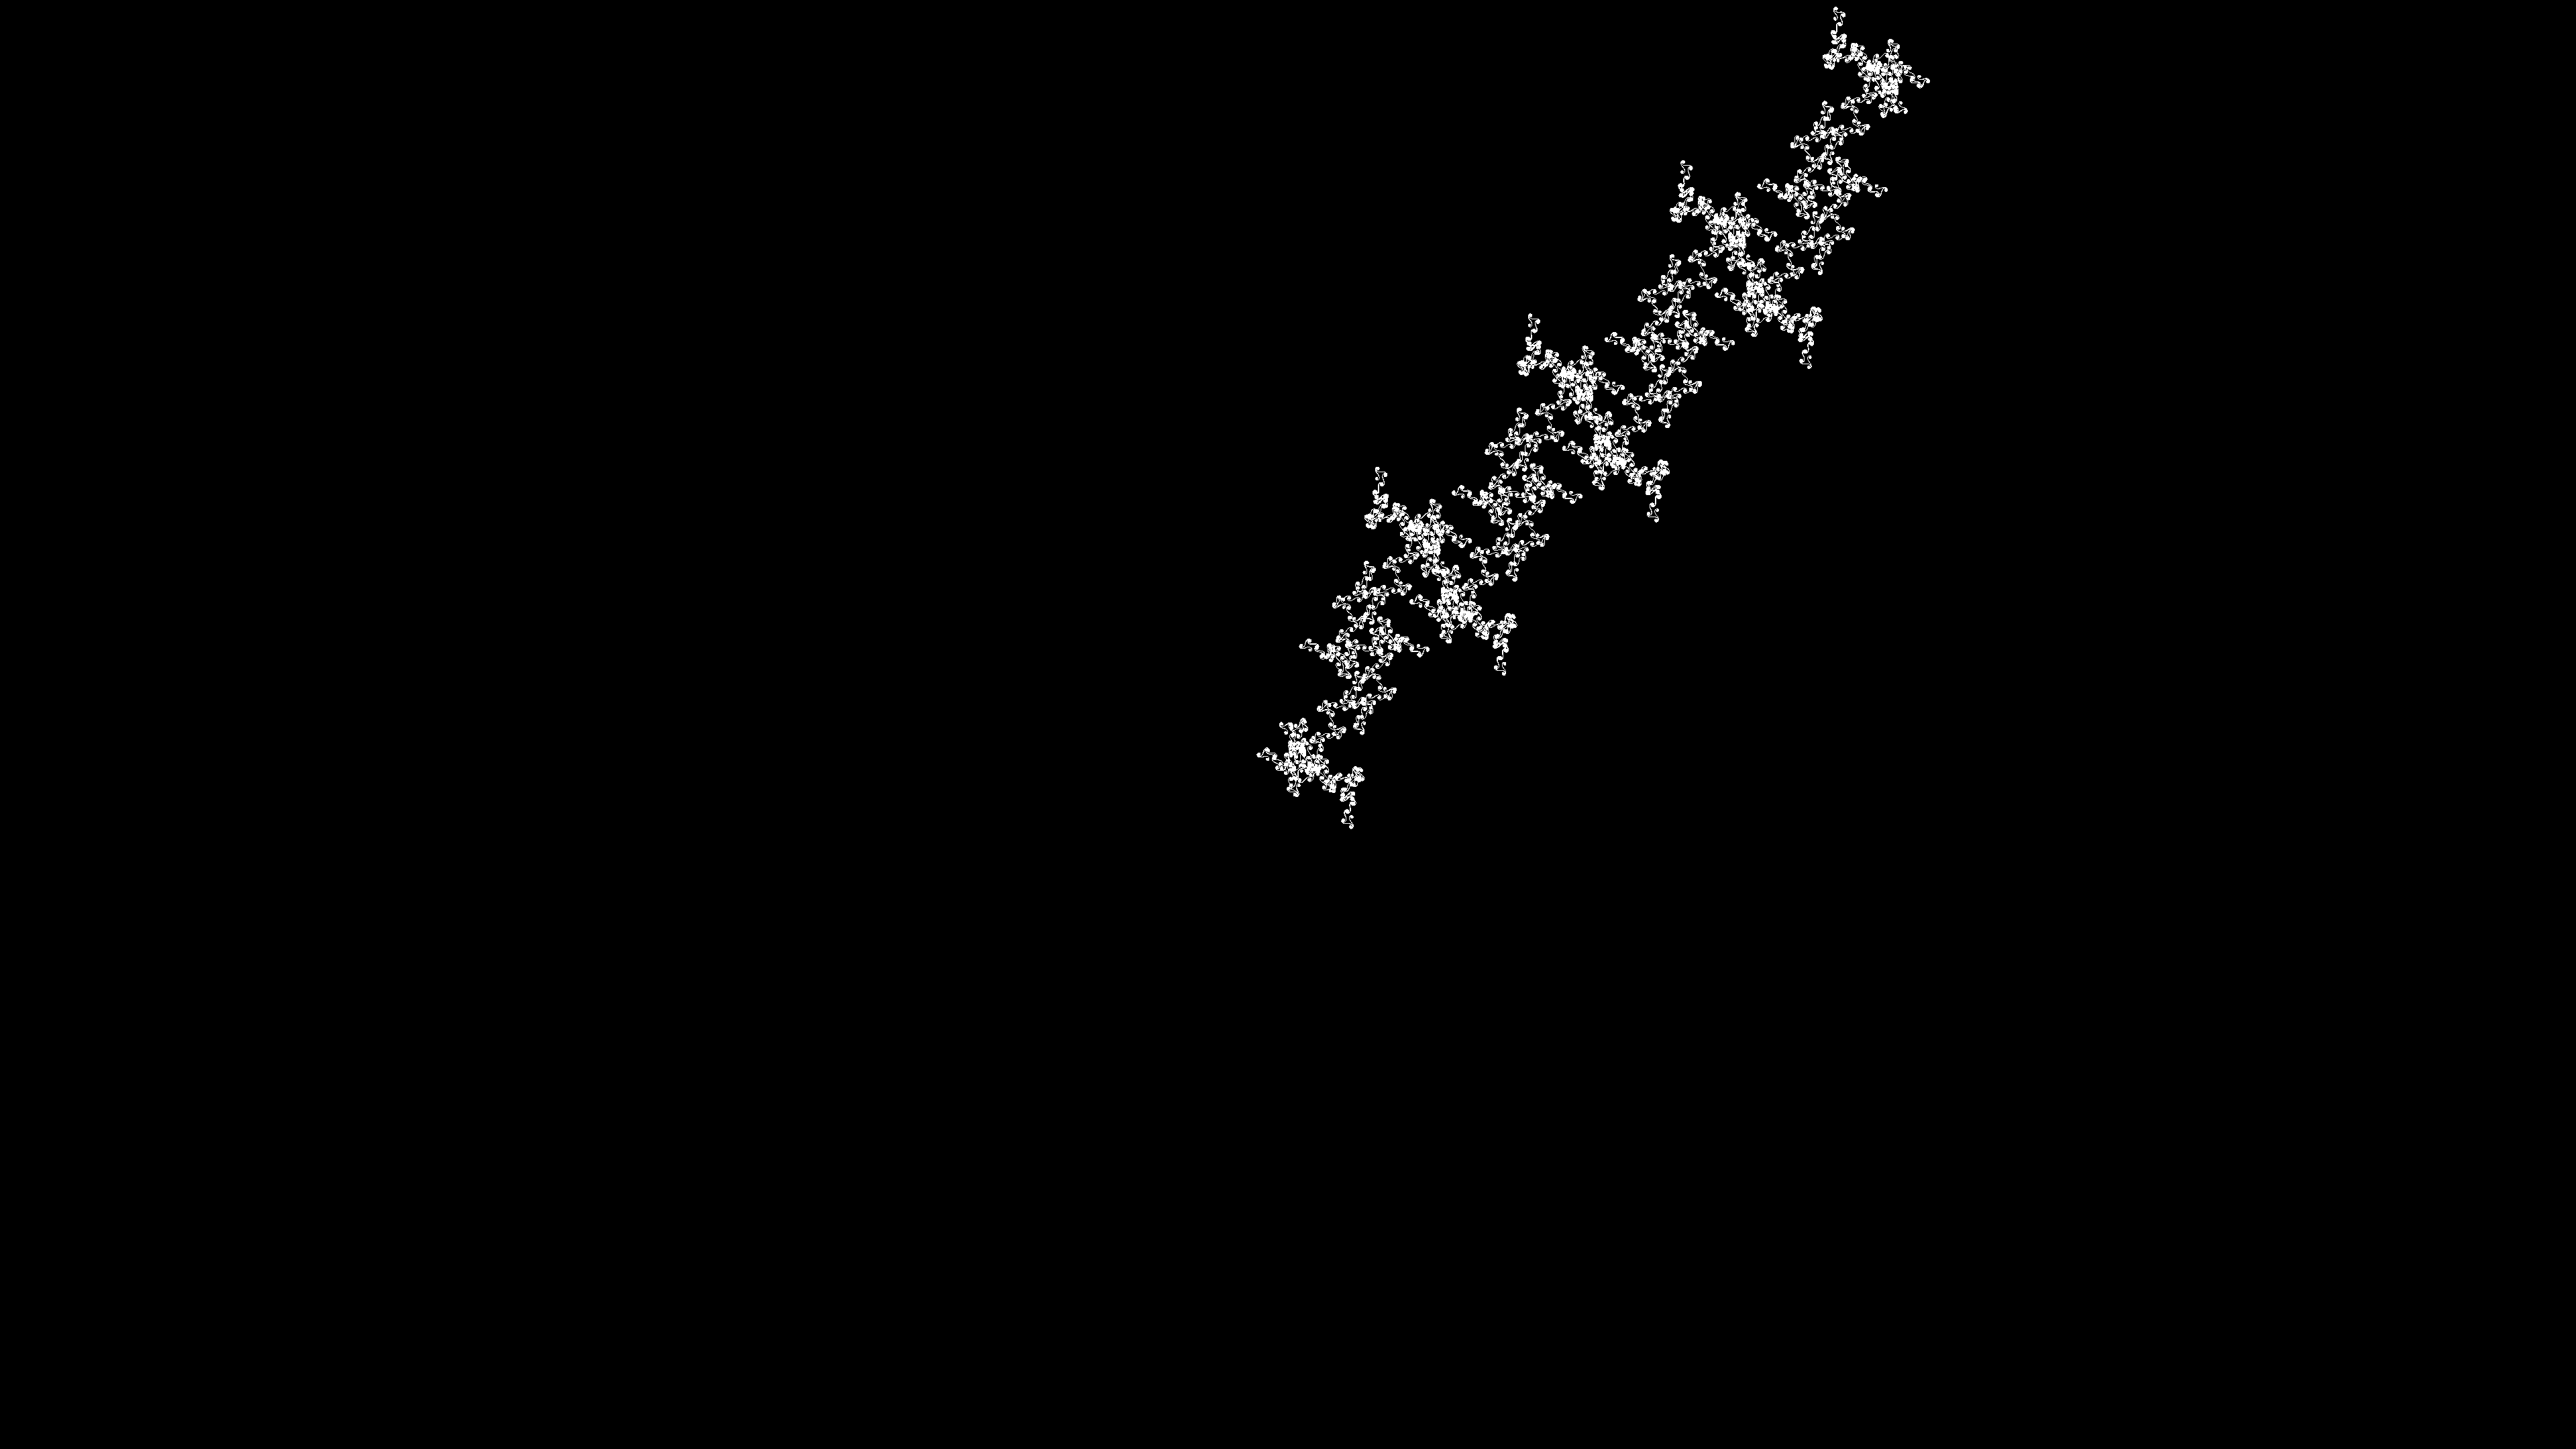
\includegraphics[width=\linewidth]{./stepsplusoneimages/0000000078.png}
    \caption{tf p=499 q=200175 theta=000 89741476.png}
  \end{subfigure}
  \caption{n=076 s=400 s+1=401}
  \label{fig:n=076}
\end{figure}
\begin{figure}[H]
  \centering
  \begin{subfigure}[t]{0.48\textwidth}
    \centering
    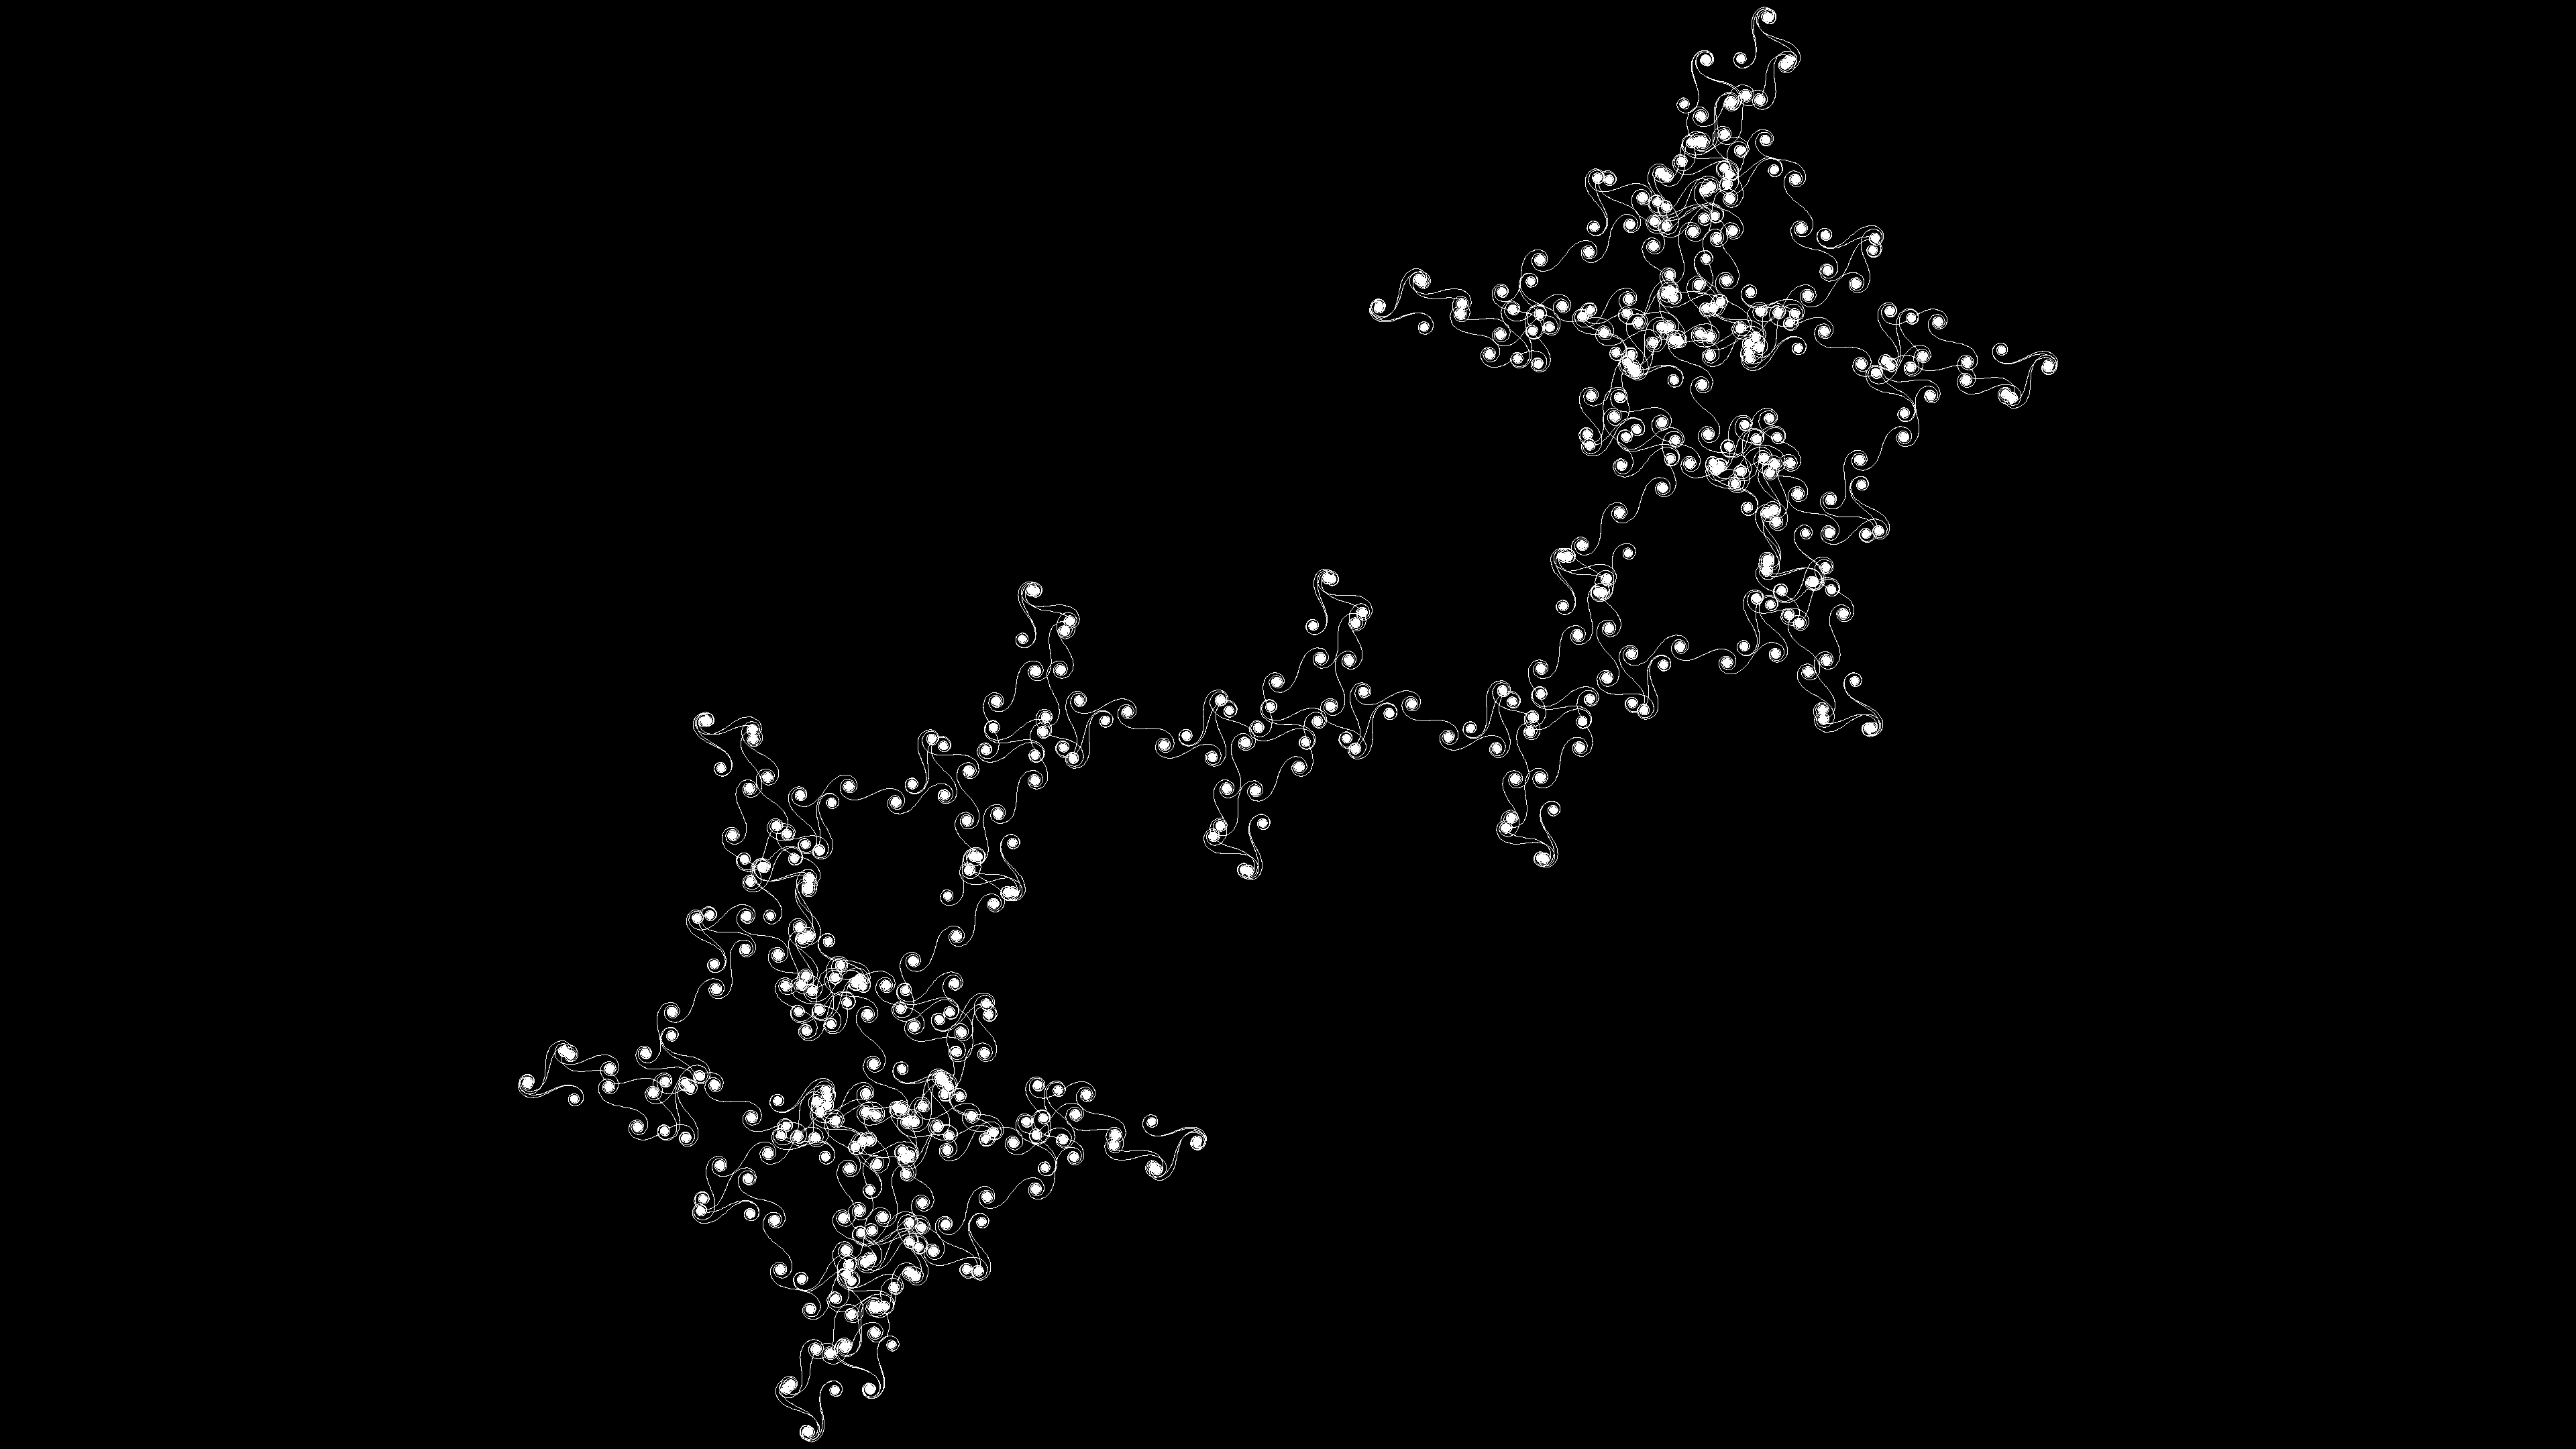
\includegraphics[width=\linewidth]{./stepsplusoneimages/0000000079.png}
    \caption{tf p=499 q=199678 theta=000 89964843.png}
  \end{subfigure}
  \begin{subfigure}[t]{0.48\textwidth}
    \centering
    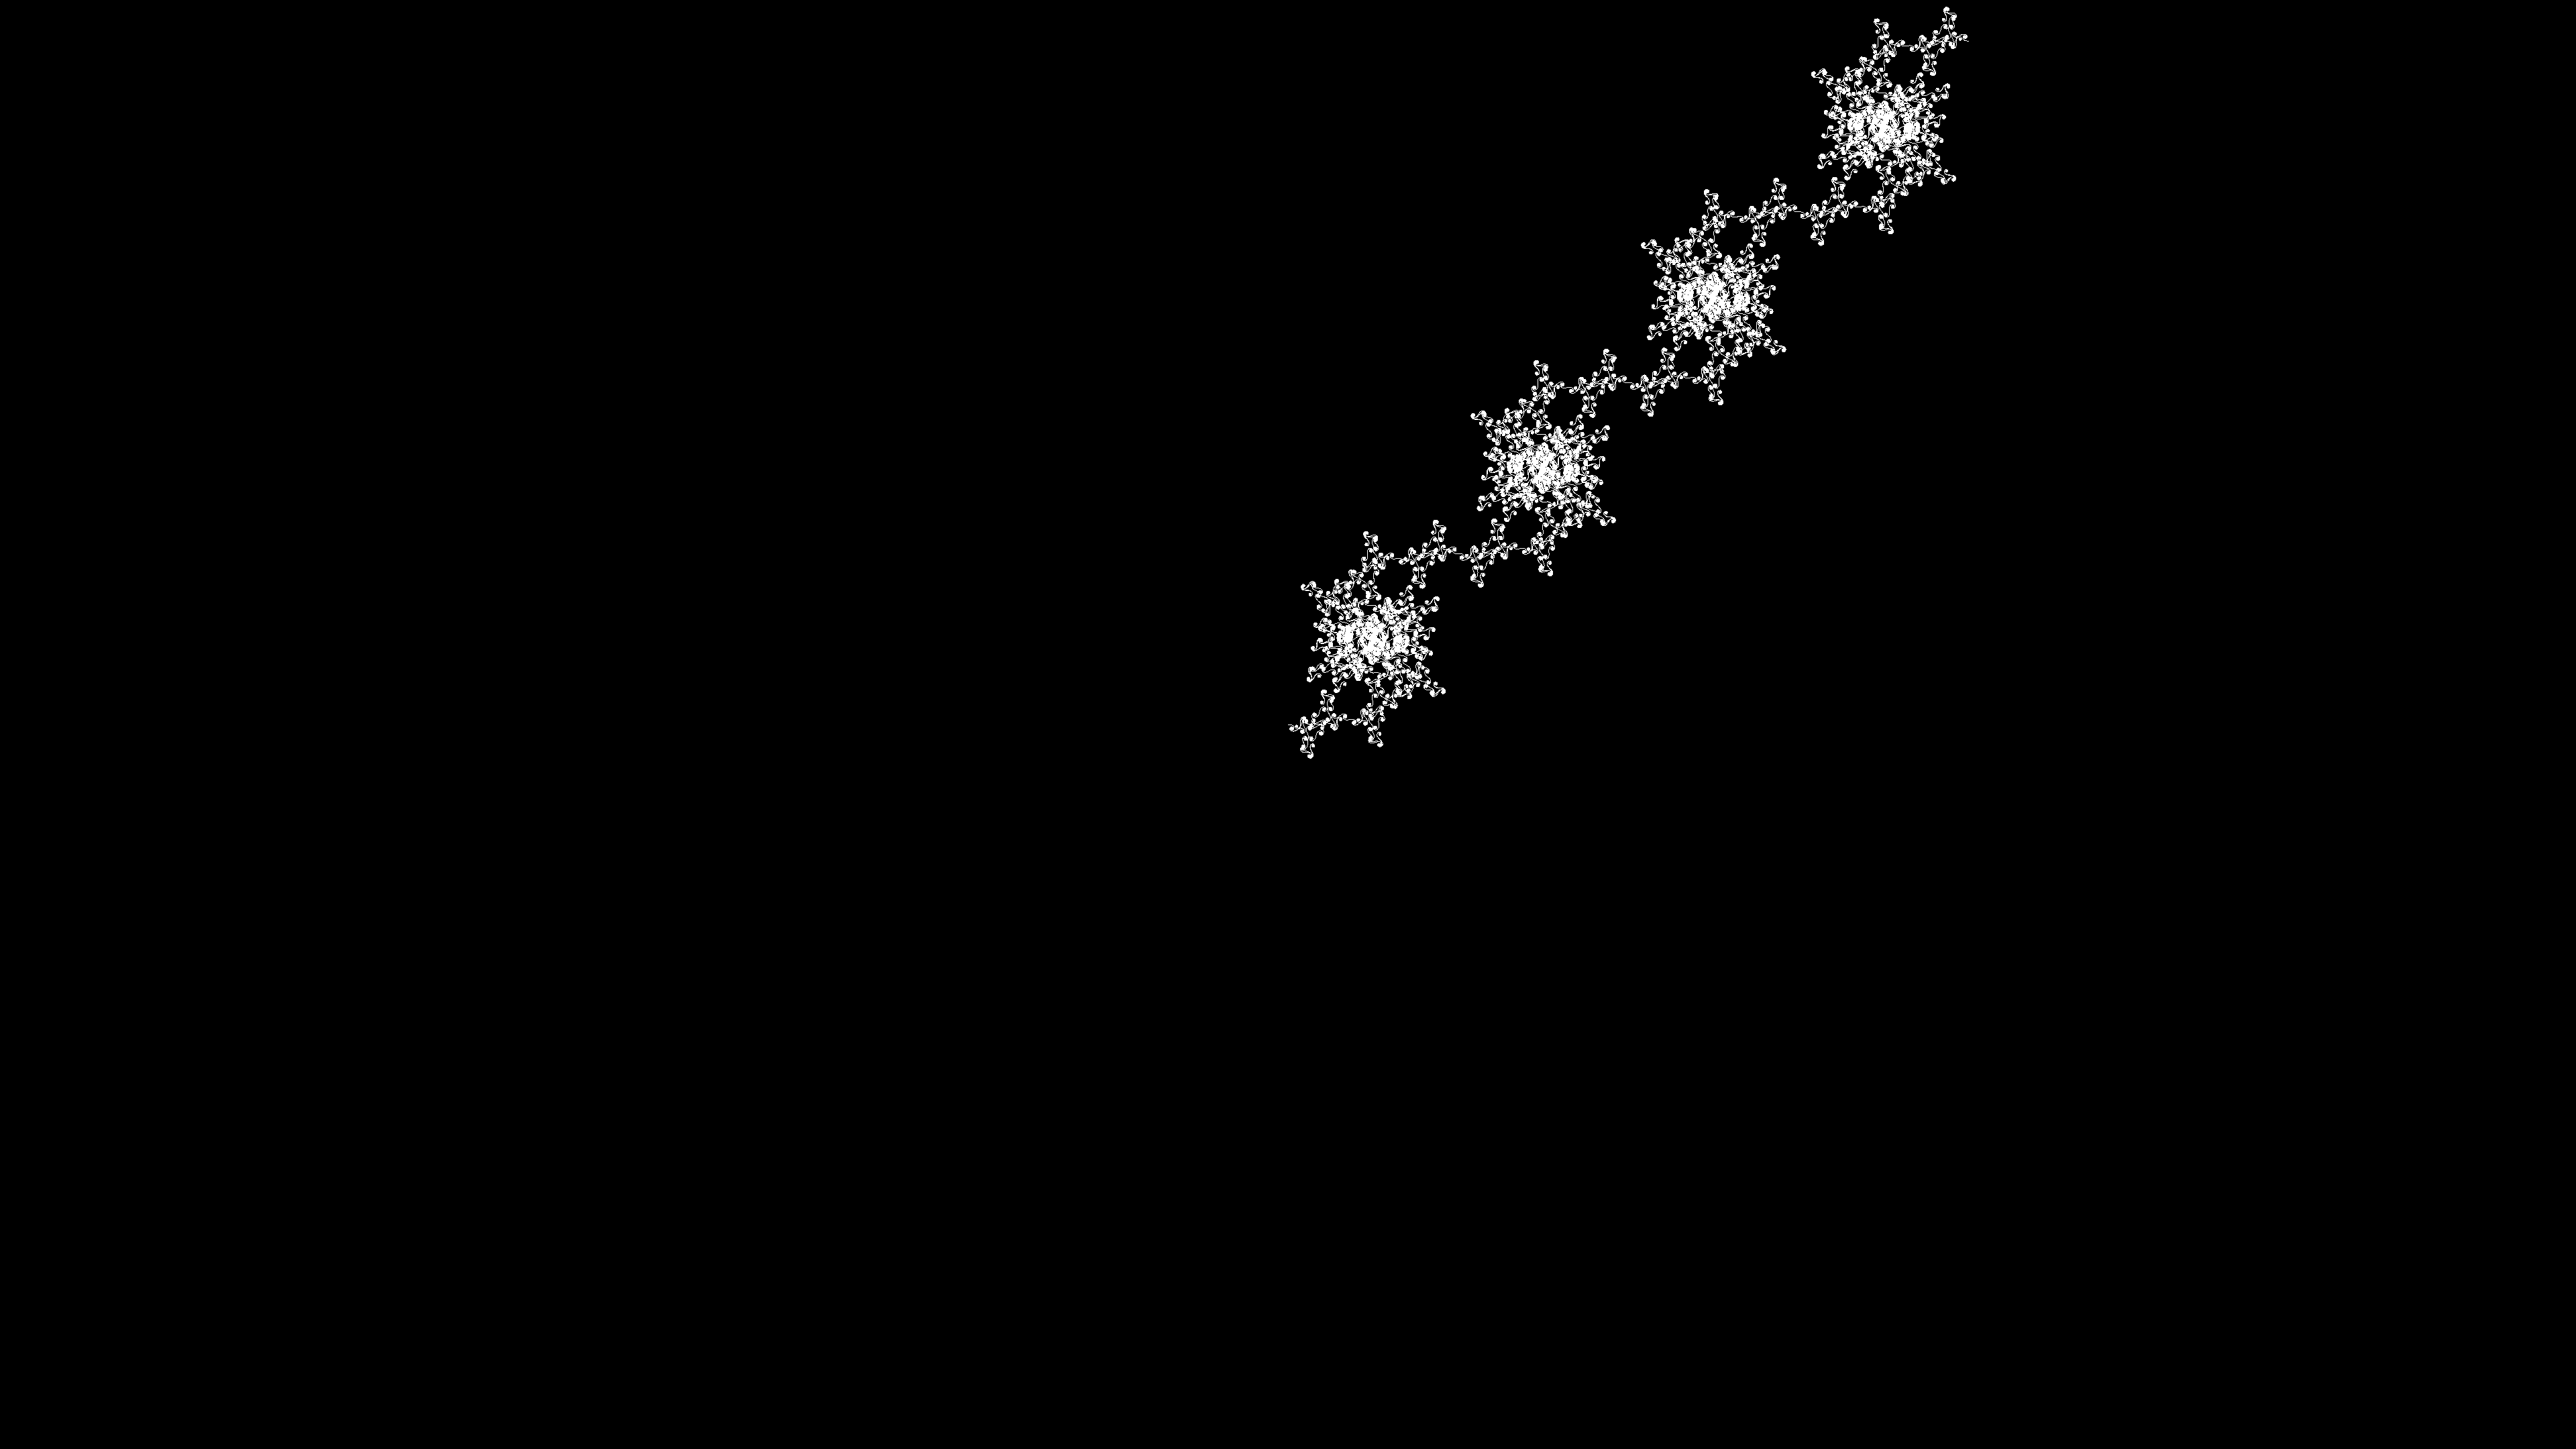
\includegraphics[width=\linewidth]{./stepsplusoneimages/0000000080.png}
    \caption{tf p=499 q=200177 theta=000 89740580.png}
  \end{subfigure}
  \caption{n=078 s=400 s+1=401}
  \label{fig:n=078}
\end{figure}
\begin{figure}[H]
  \centering
  \begin{subfigure}[t]{0.48\textwidth}
    \centering
    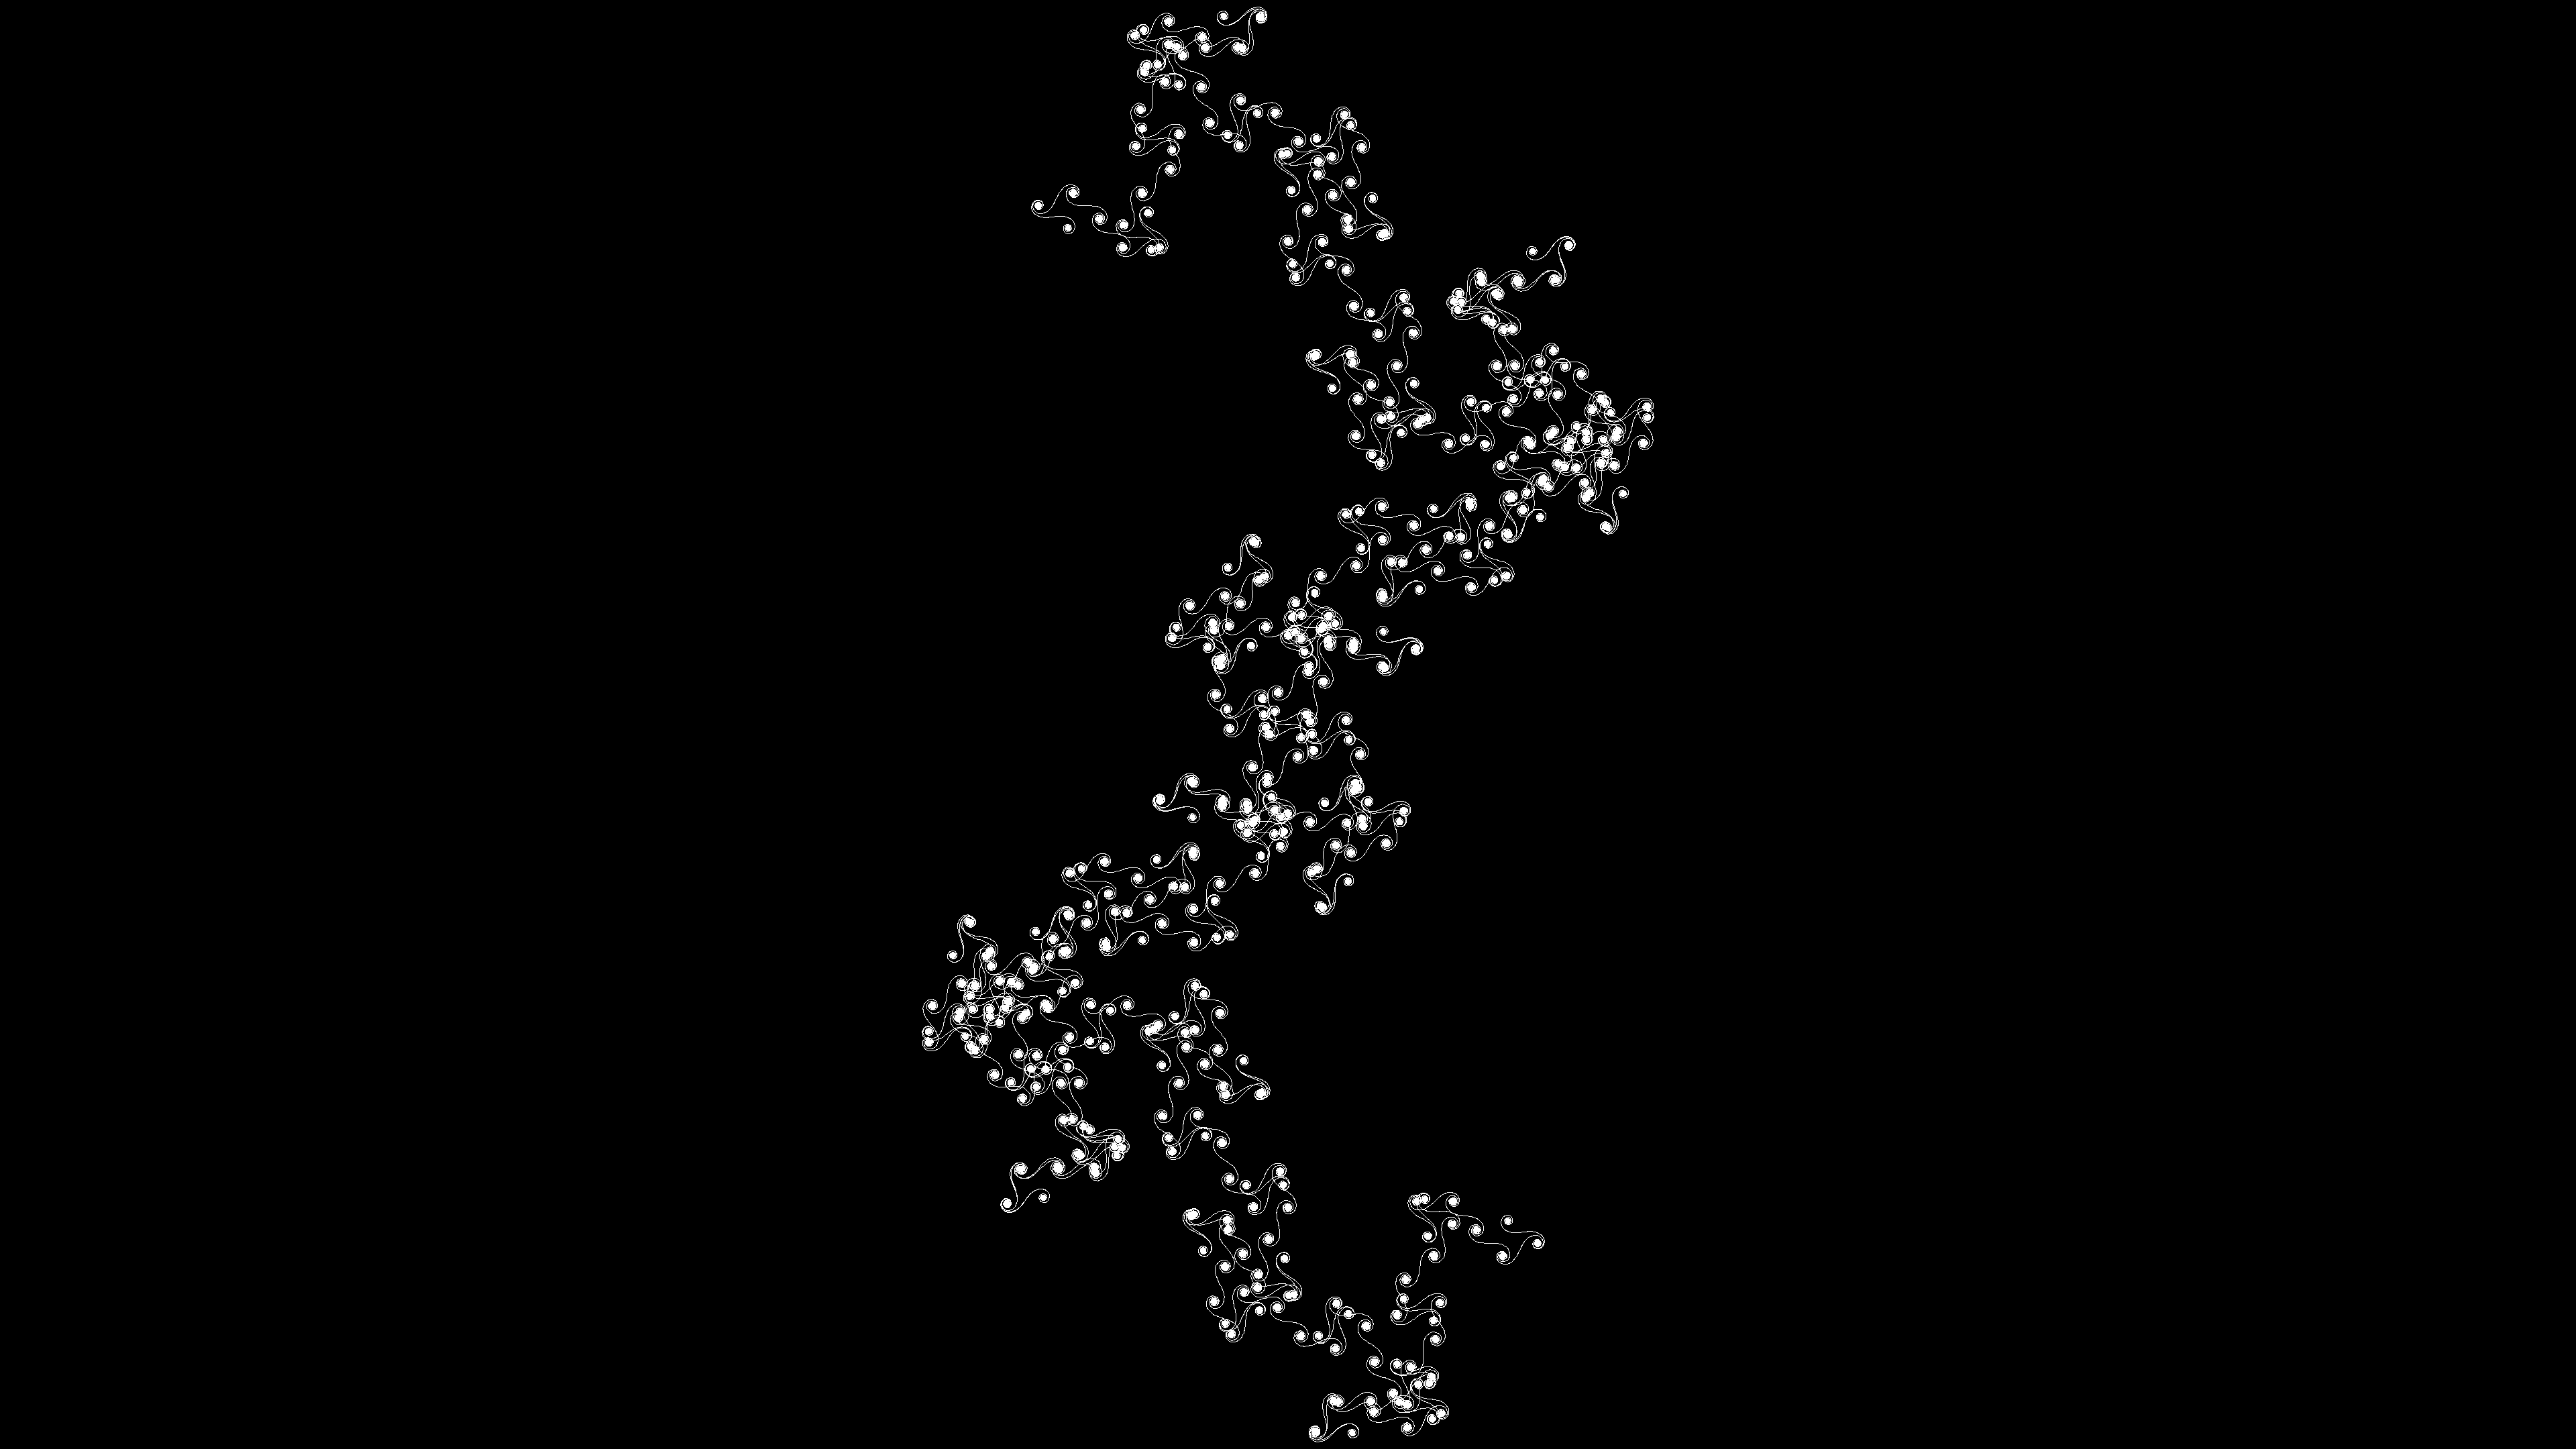
\includegraphics[width=\linewidth]{./stepsplusoneimages/0000000081.png}
    \caption{tf p=499 q=199680 theta=000 89963942.png}
  \end{subfigure}
  \begin{subfigure}[t]{0.48\textwidth}
    \centering
    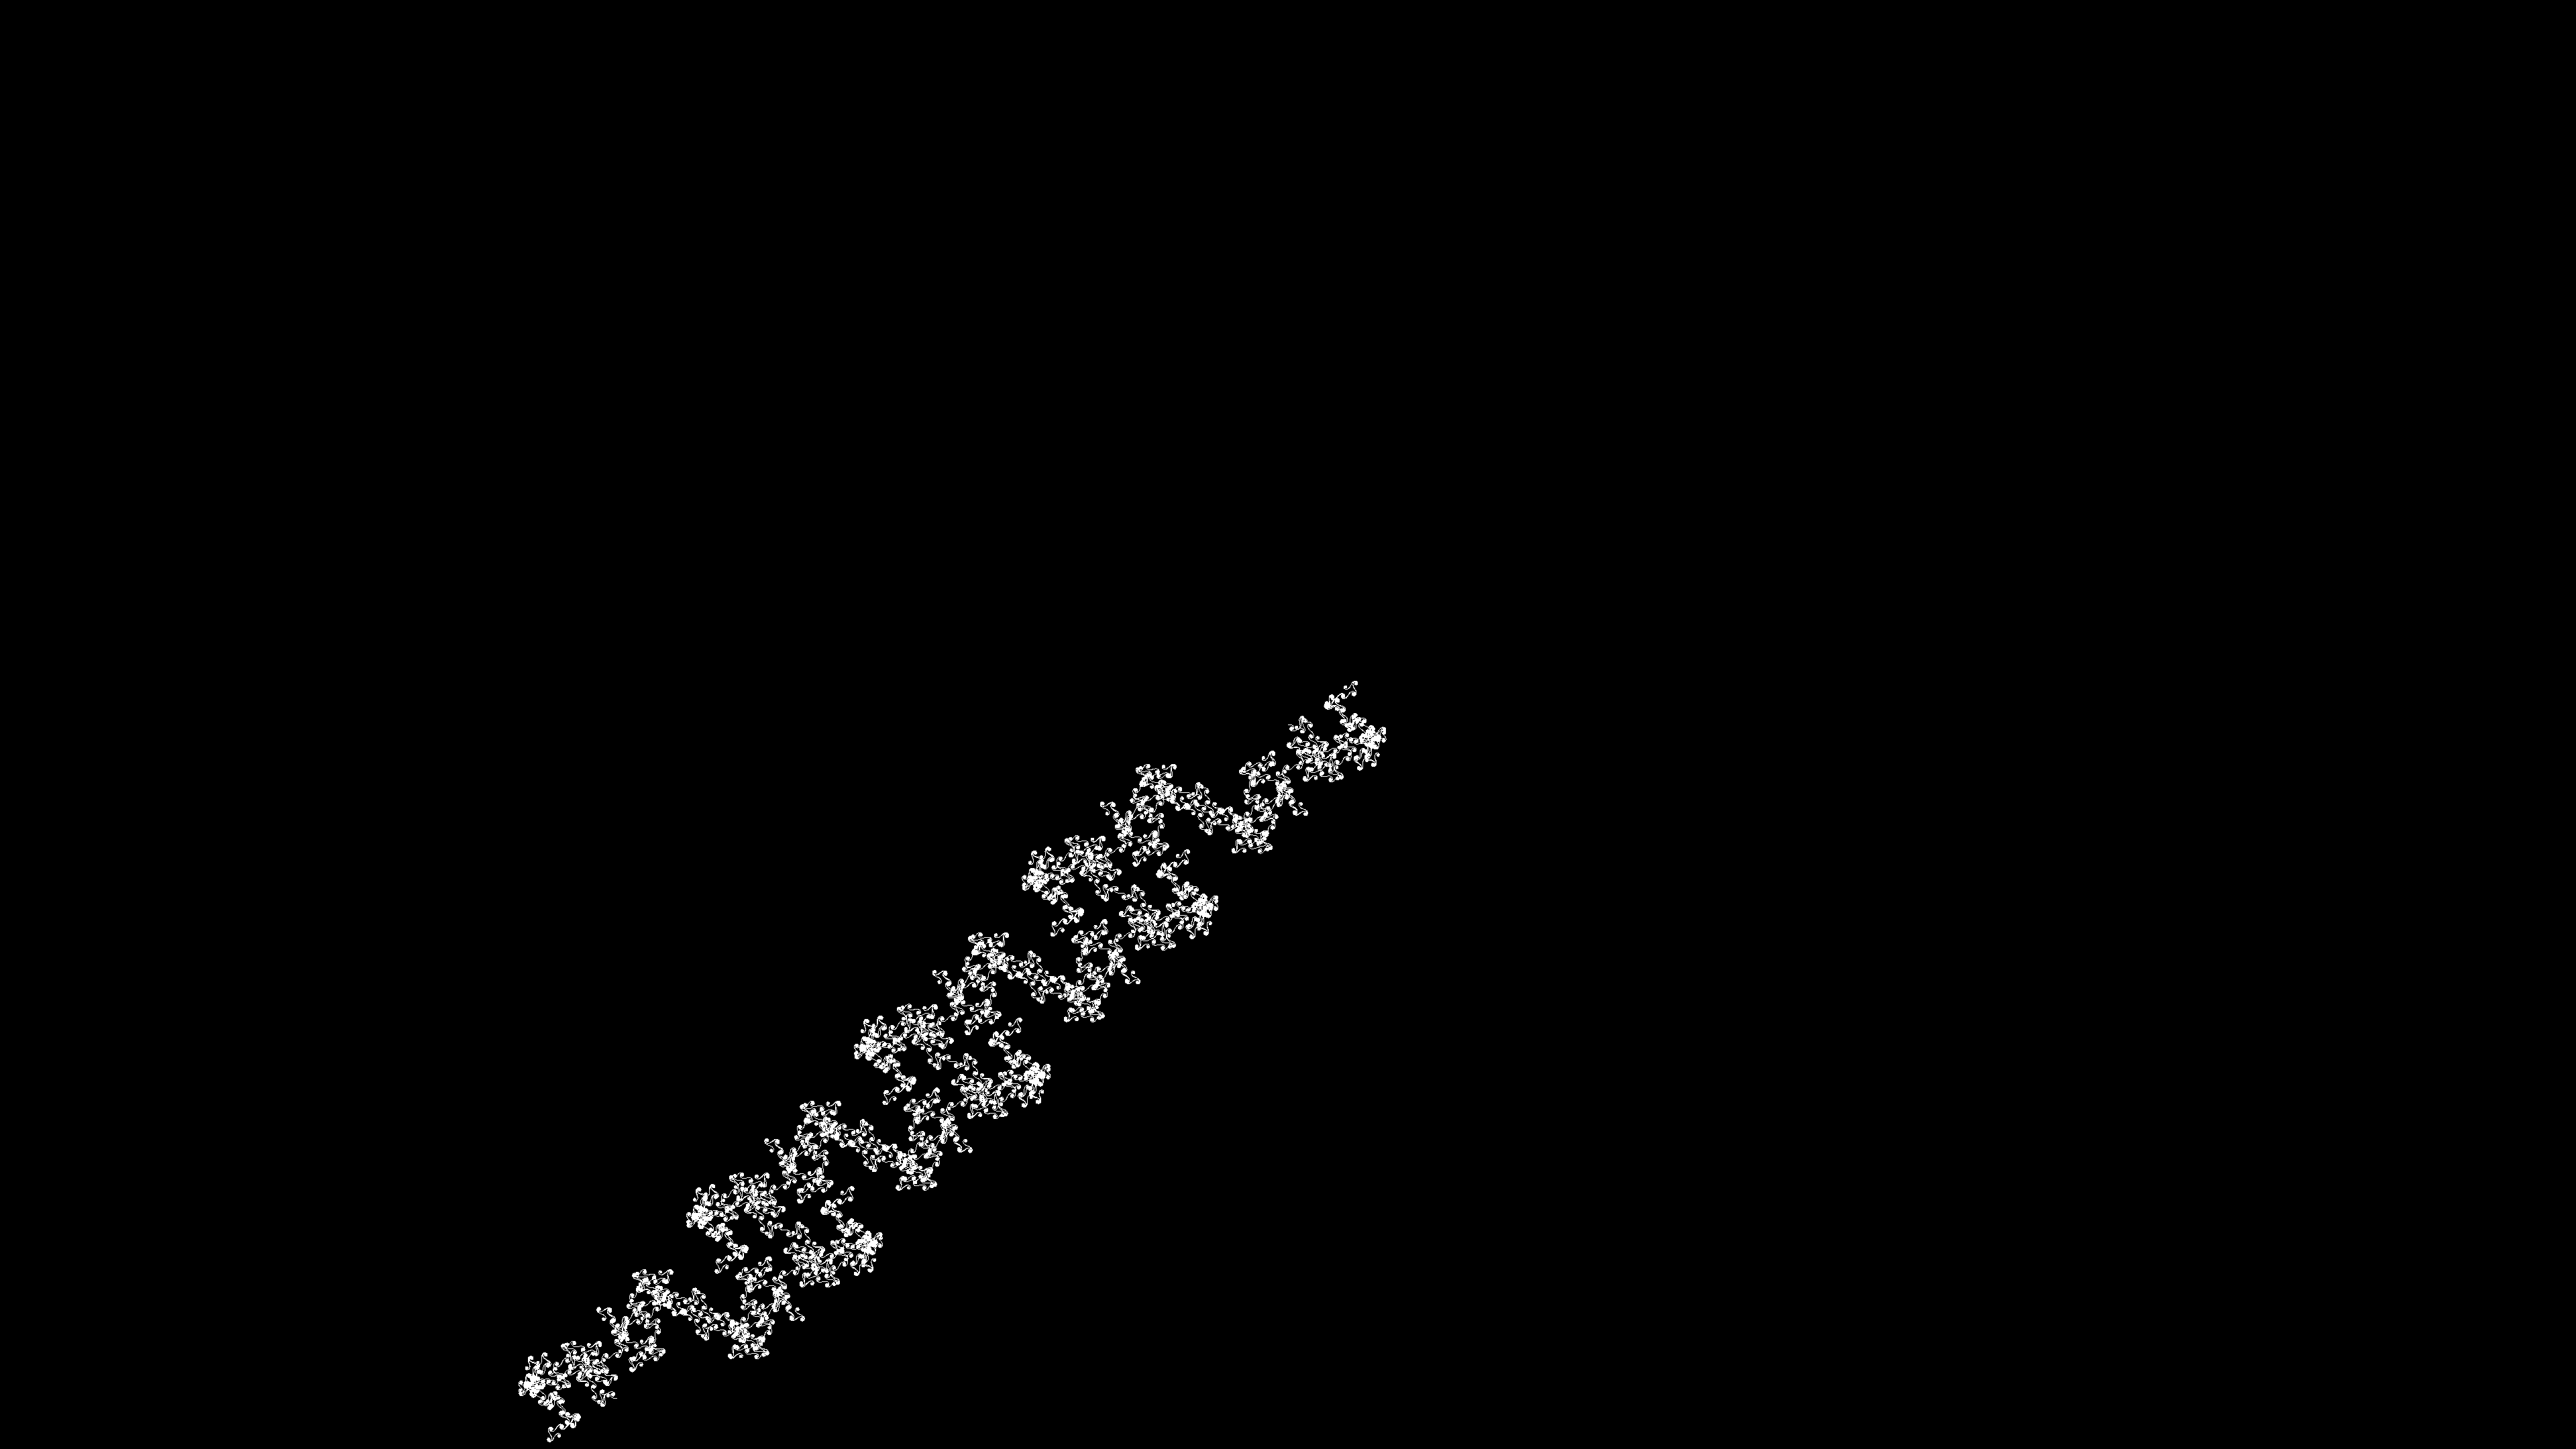
\includegraphics[width=\linewidth]{./stepsplusoneimages/0000000082.png}
    \caption{tf p=499 q=200179 theta=000 89739683.png}
  \end{subfigure}
  \caption{n=080 s=400 s+1=401}
  \label{fig:n=080}
\end{figure}
\begin{figure}[H]
  \centering
  \begin{subfigure}[t]{0.48\textwidth}
    \centering
    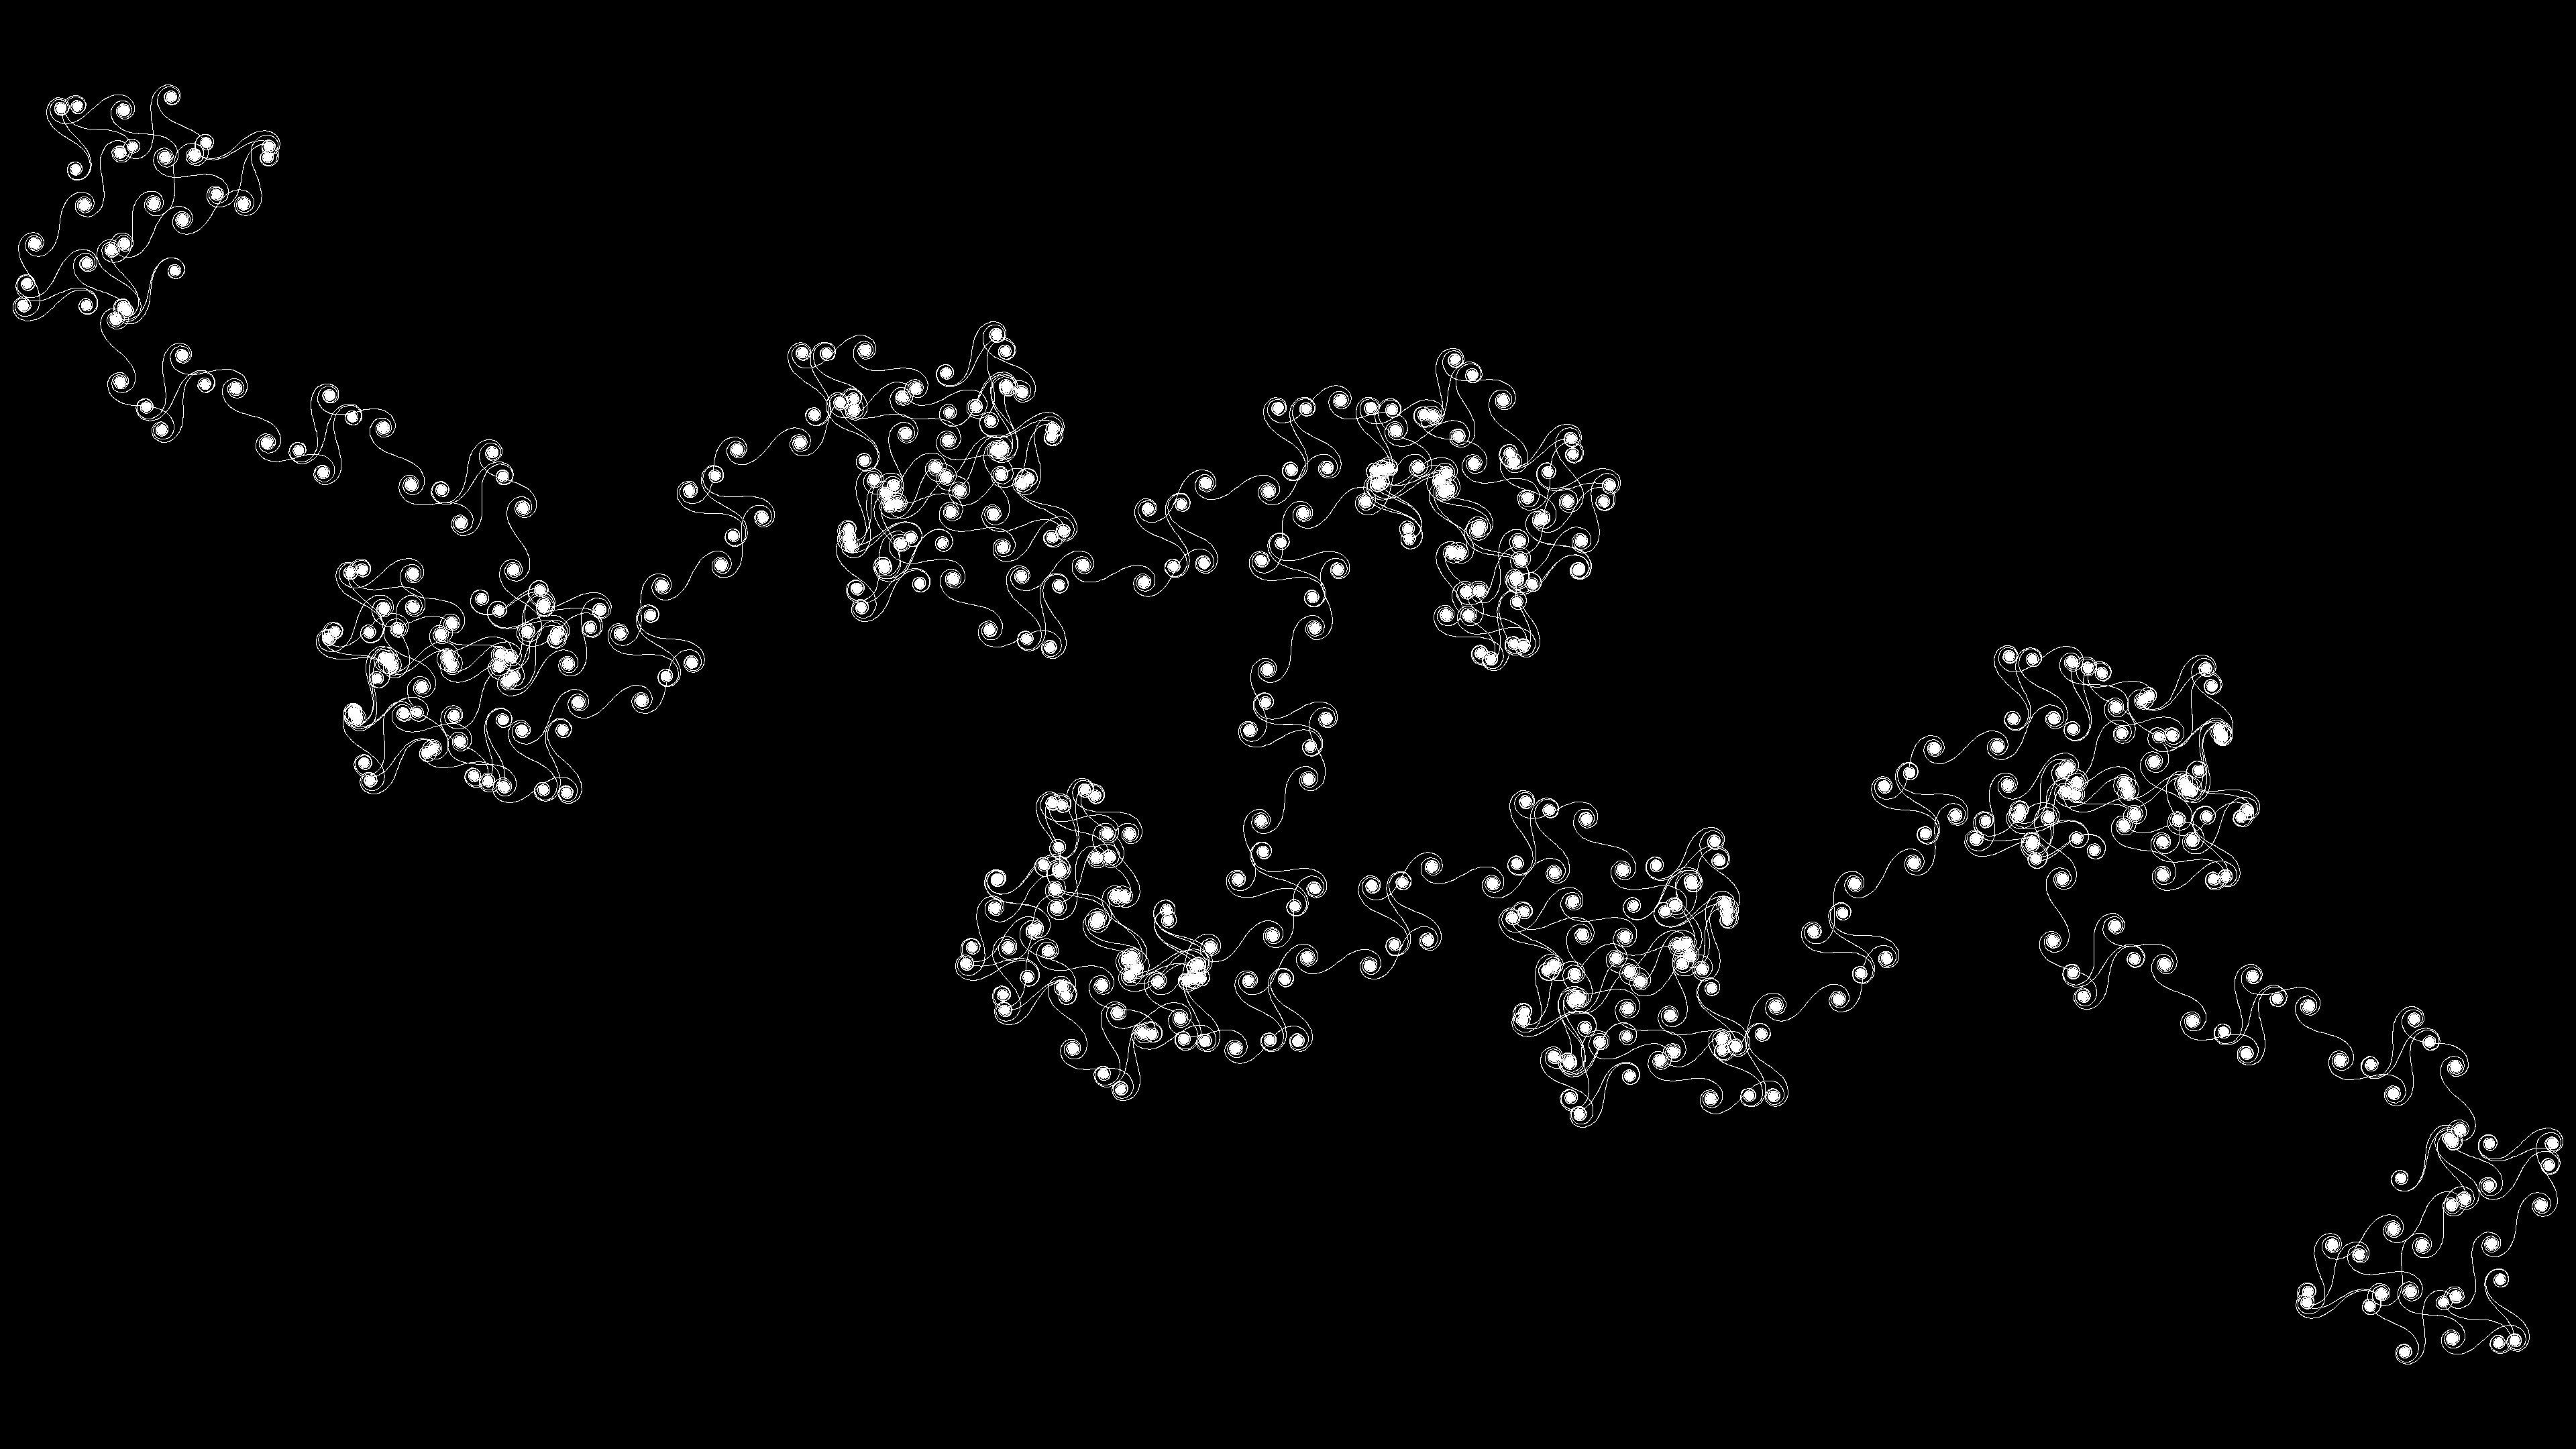
\includegraphics[width=\linewidth]{./stepsplusoneimages/0000000083.png}
    \caption{tf p=499 q=199682 theta=000 89963041.png}
  \end{subfigure}
  \begin{subfigure}[t]{0.48\textwidth}
    \centering
    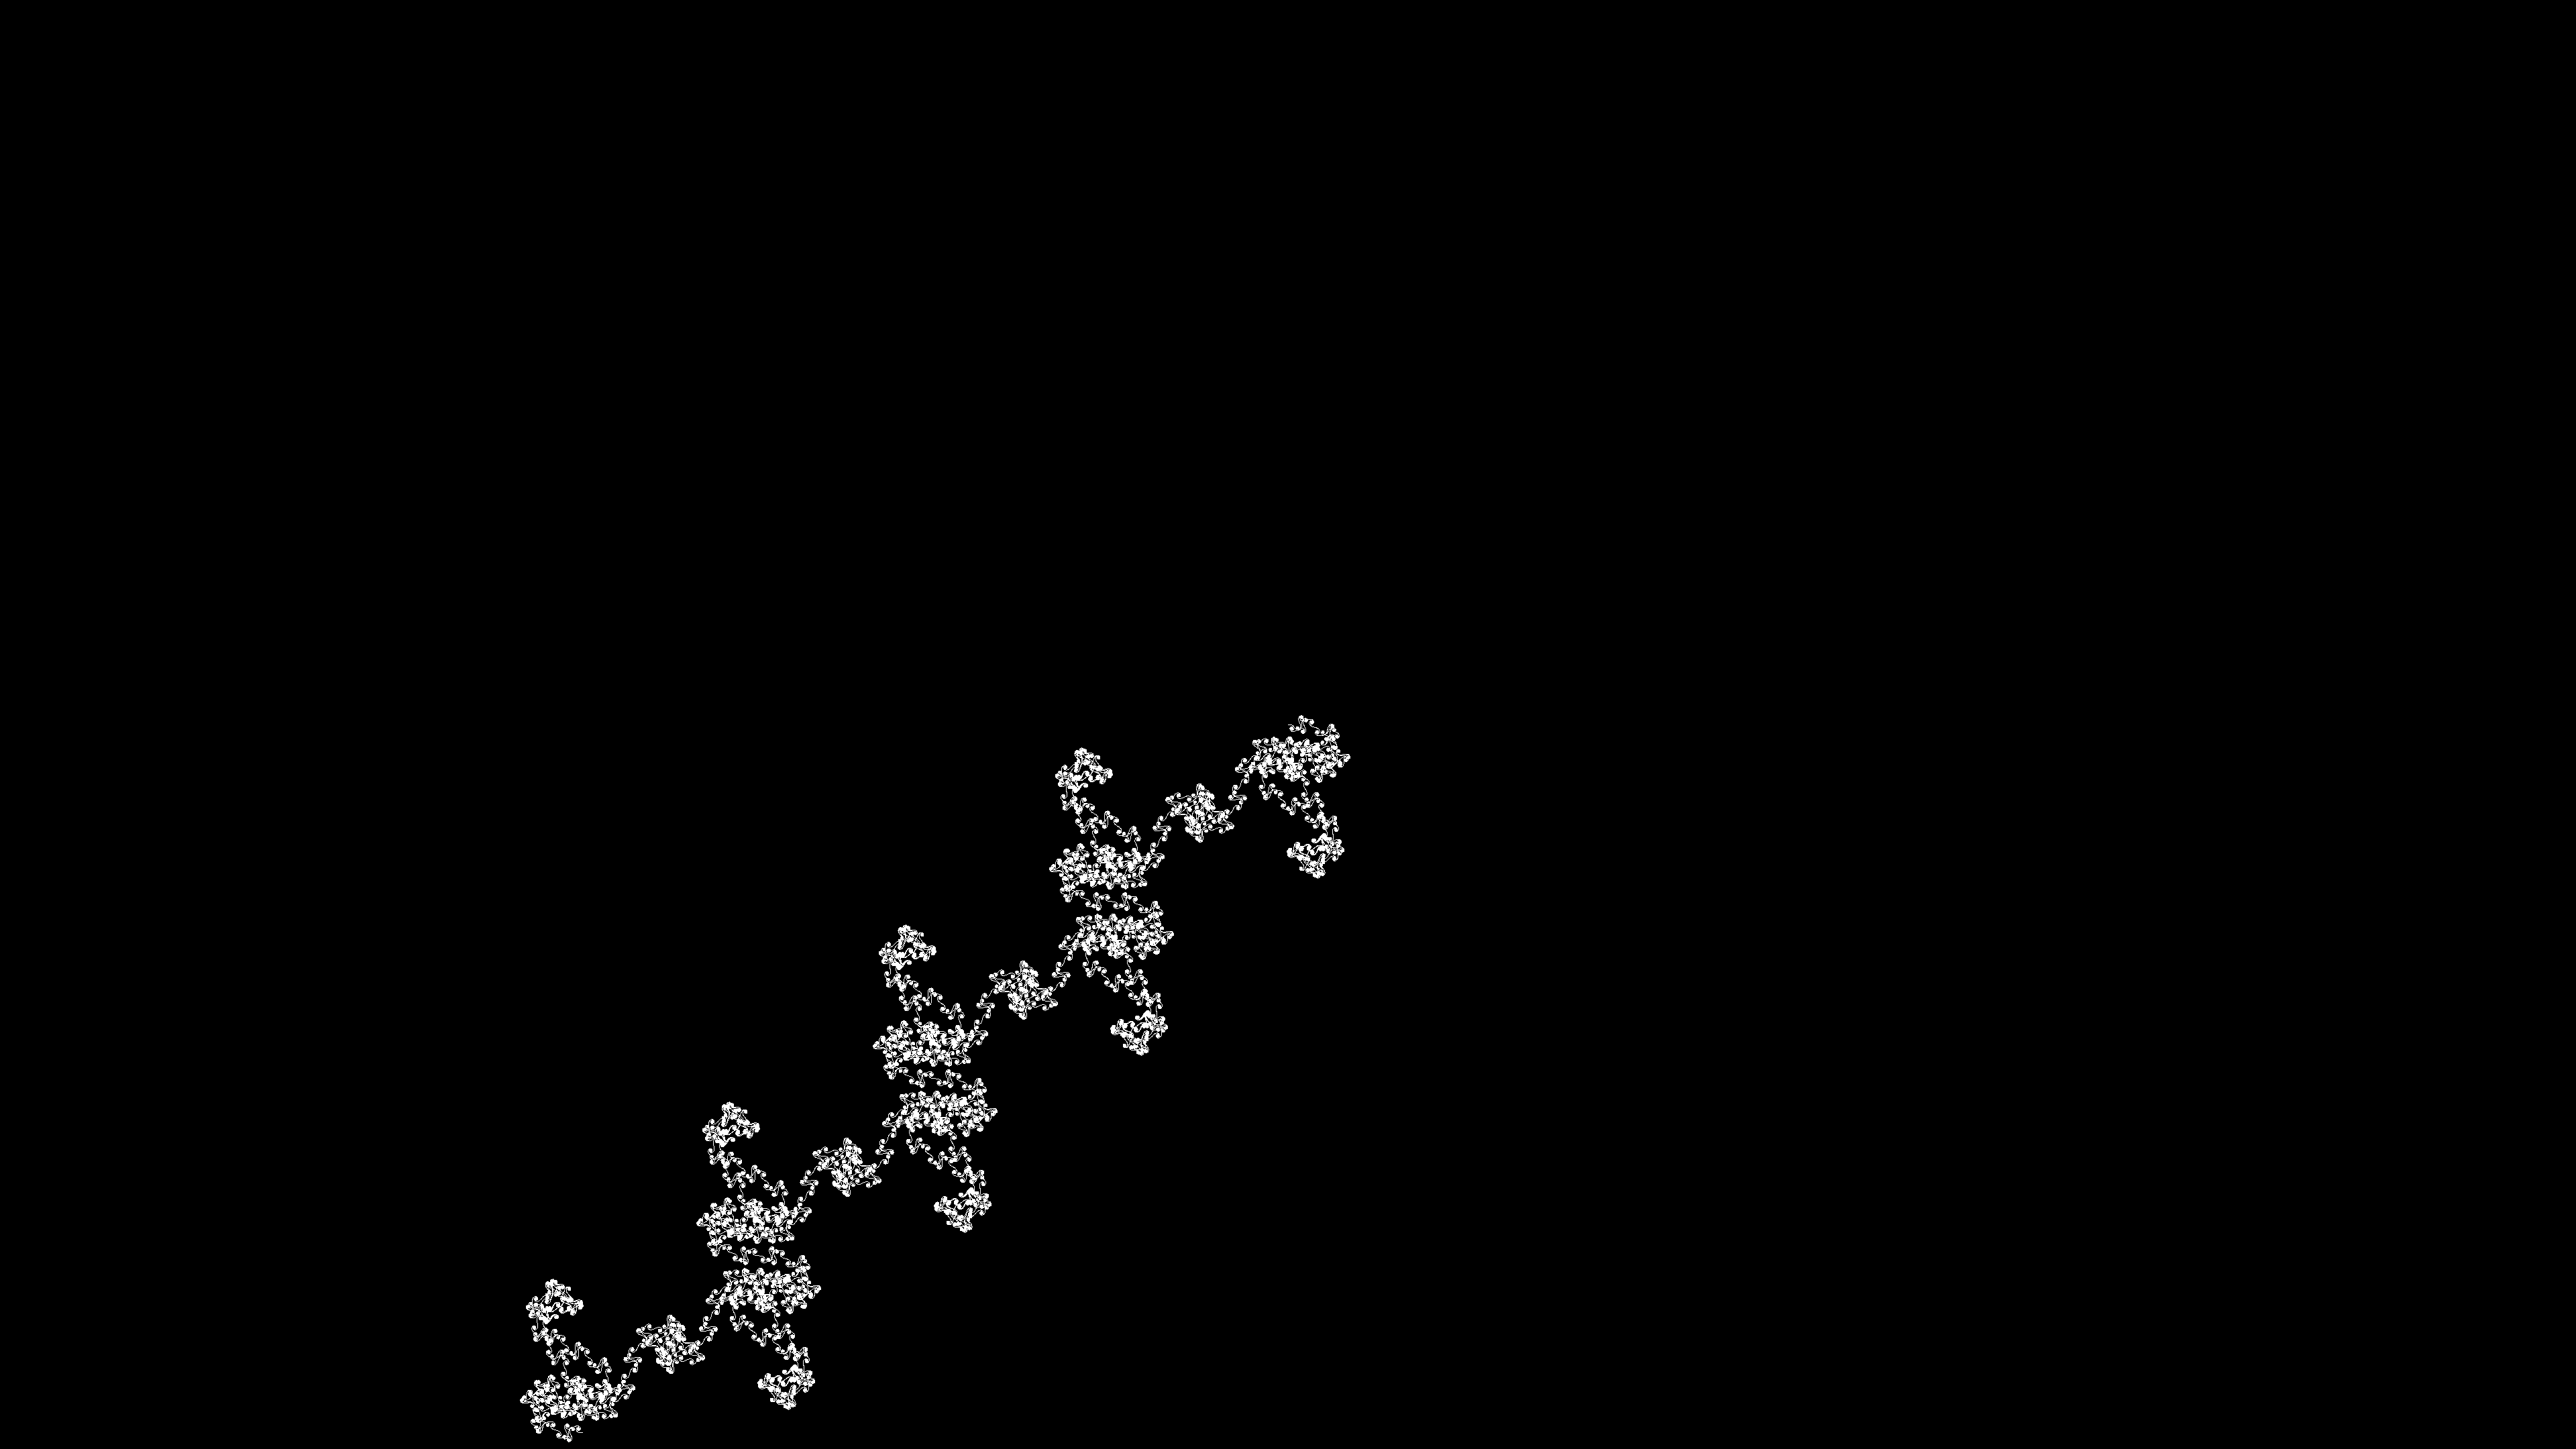
\includegraphics[width=\linewidth]{./stepsplusoneimages/0000000084.png}
    \caption{tf p=499 q=200181 theta=000 89738786.png}
  \end{subfigure}
  \caption{n=082 s=400 s+1=401}
  \label{fig:n=082}
\end{figure}
\begin{figure}[H]
  \centering
  \begin{subfigure}[t]{0.48\textwidth}
    \centering
    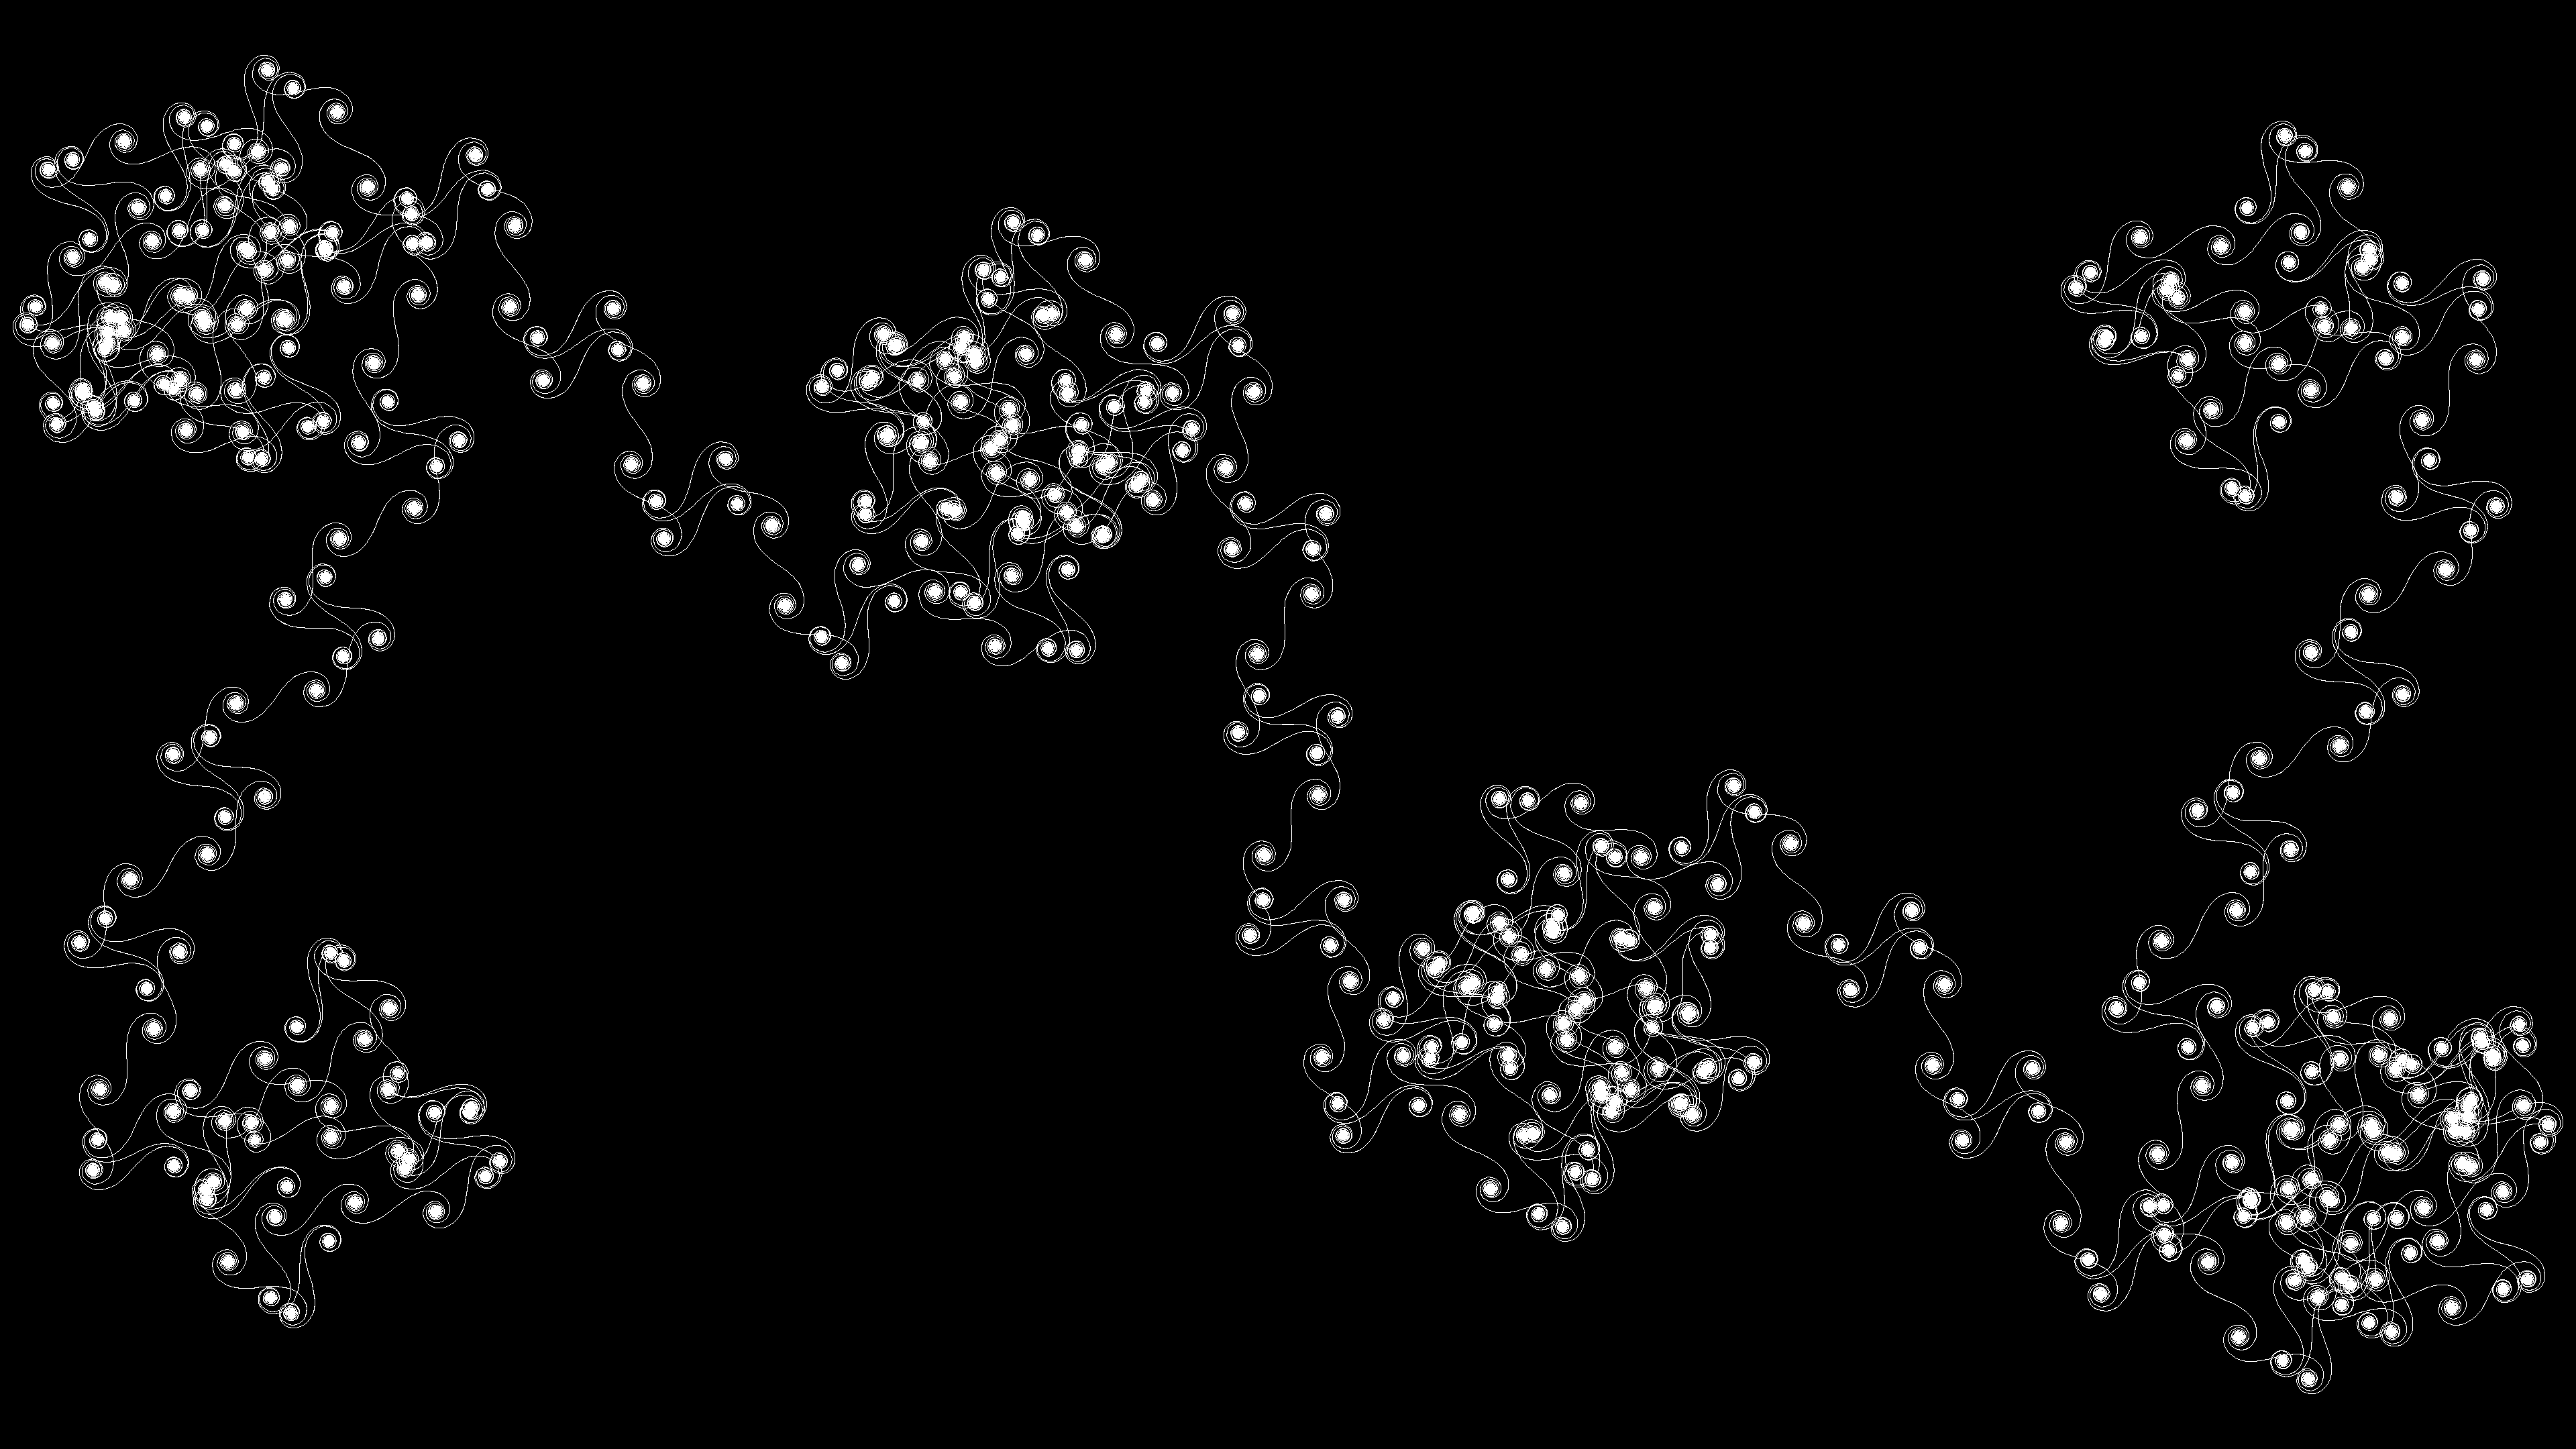
\includegraphics[width=\linewidth]{./stepsplusoneimages/0000000085.png}
    \caption{tf p=499 q=199684 theta=000 89962140.png}
  \end{subfigure}
  \begin{subfigure}[t]{0.48\textwidth}
    \centering
    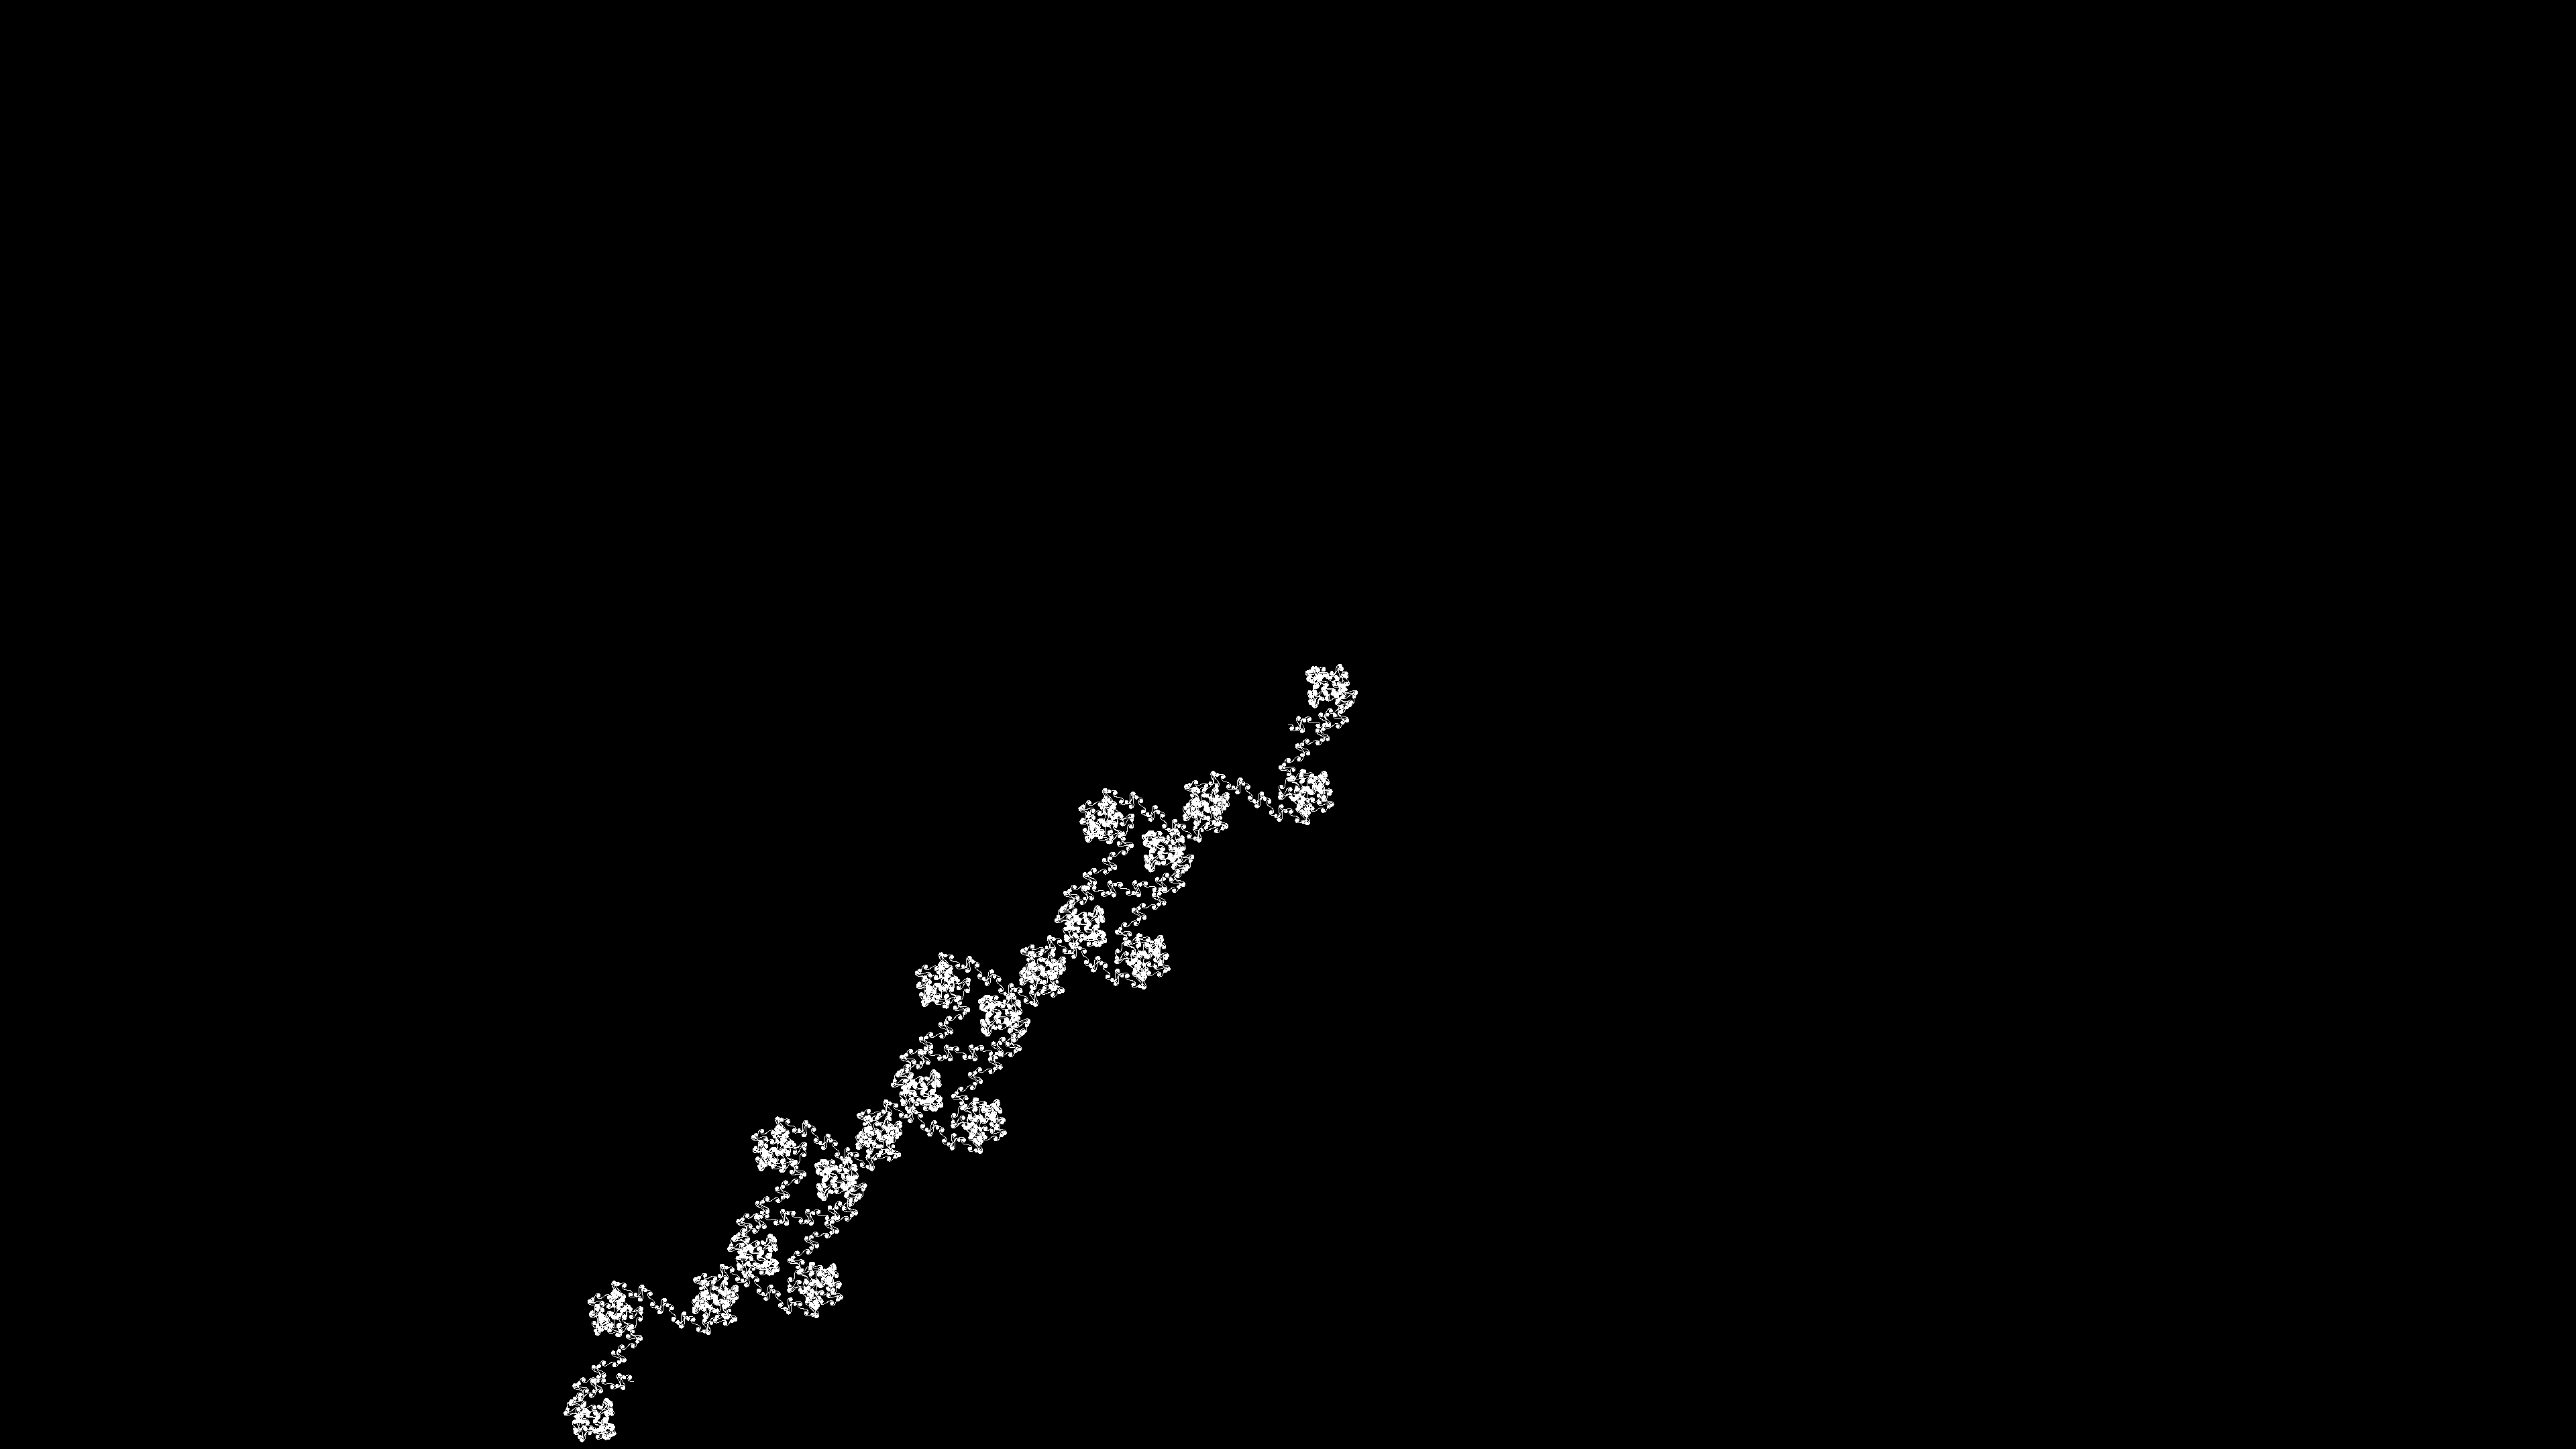
\includegraphics[width=\linewidth]{./stepsplusoneimages/0000000086.png}
    \caption{tf p=499 q=200183 theta=000 89737890.png}
  \end{subfigure}
  \caption{n=084 s=400 s+1=401}
  \label{fig:n=084}
\end{figure}
\begin{figure}[H]
  \centering
  \begin{subfigure}[t]{0.48\textwidth}
    \centering
    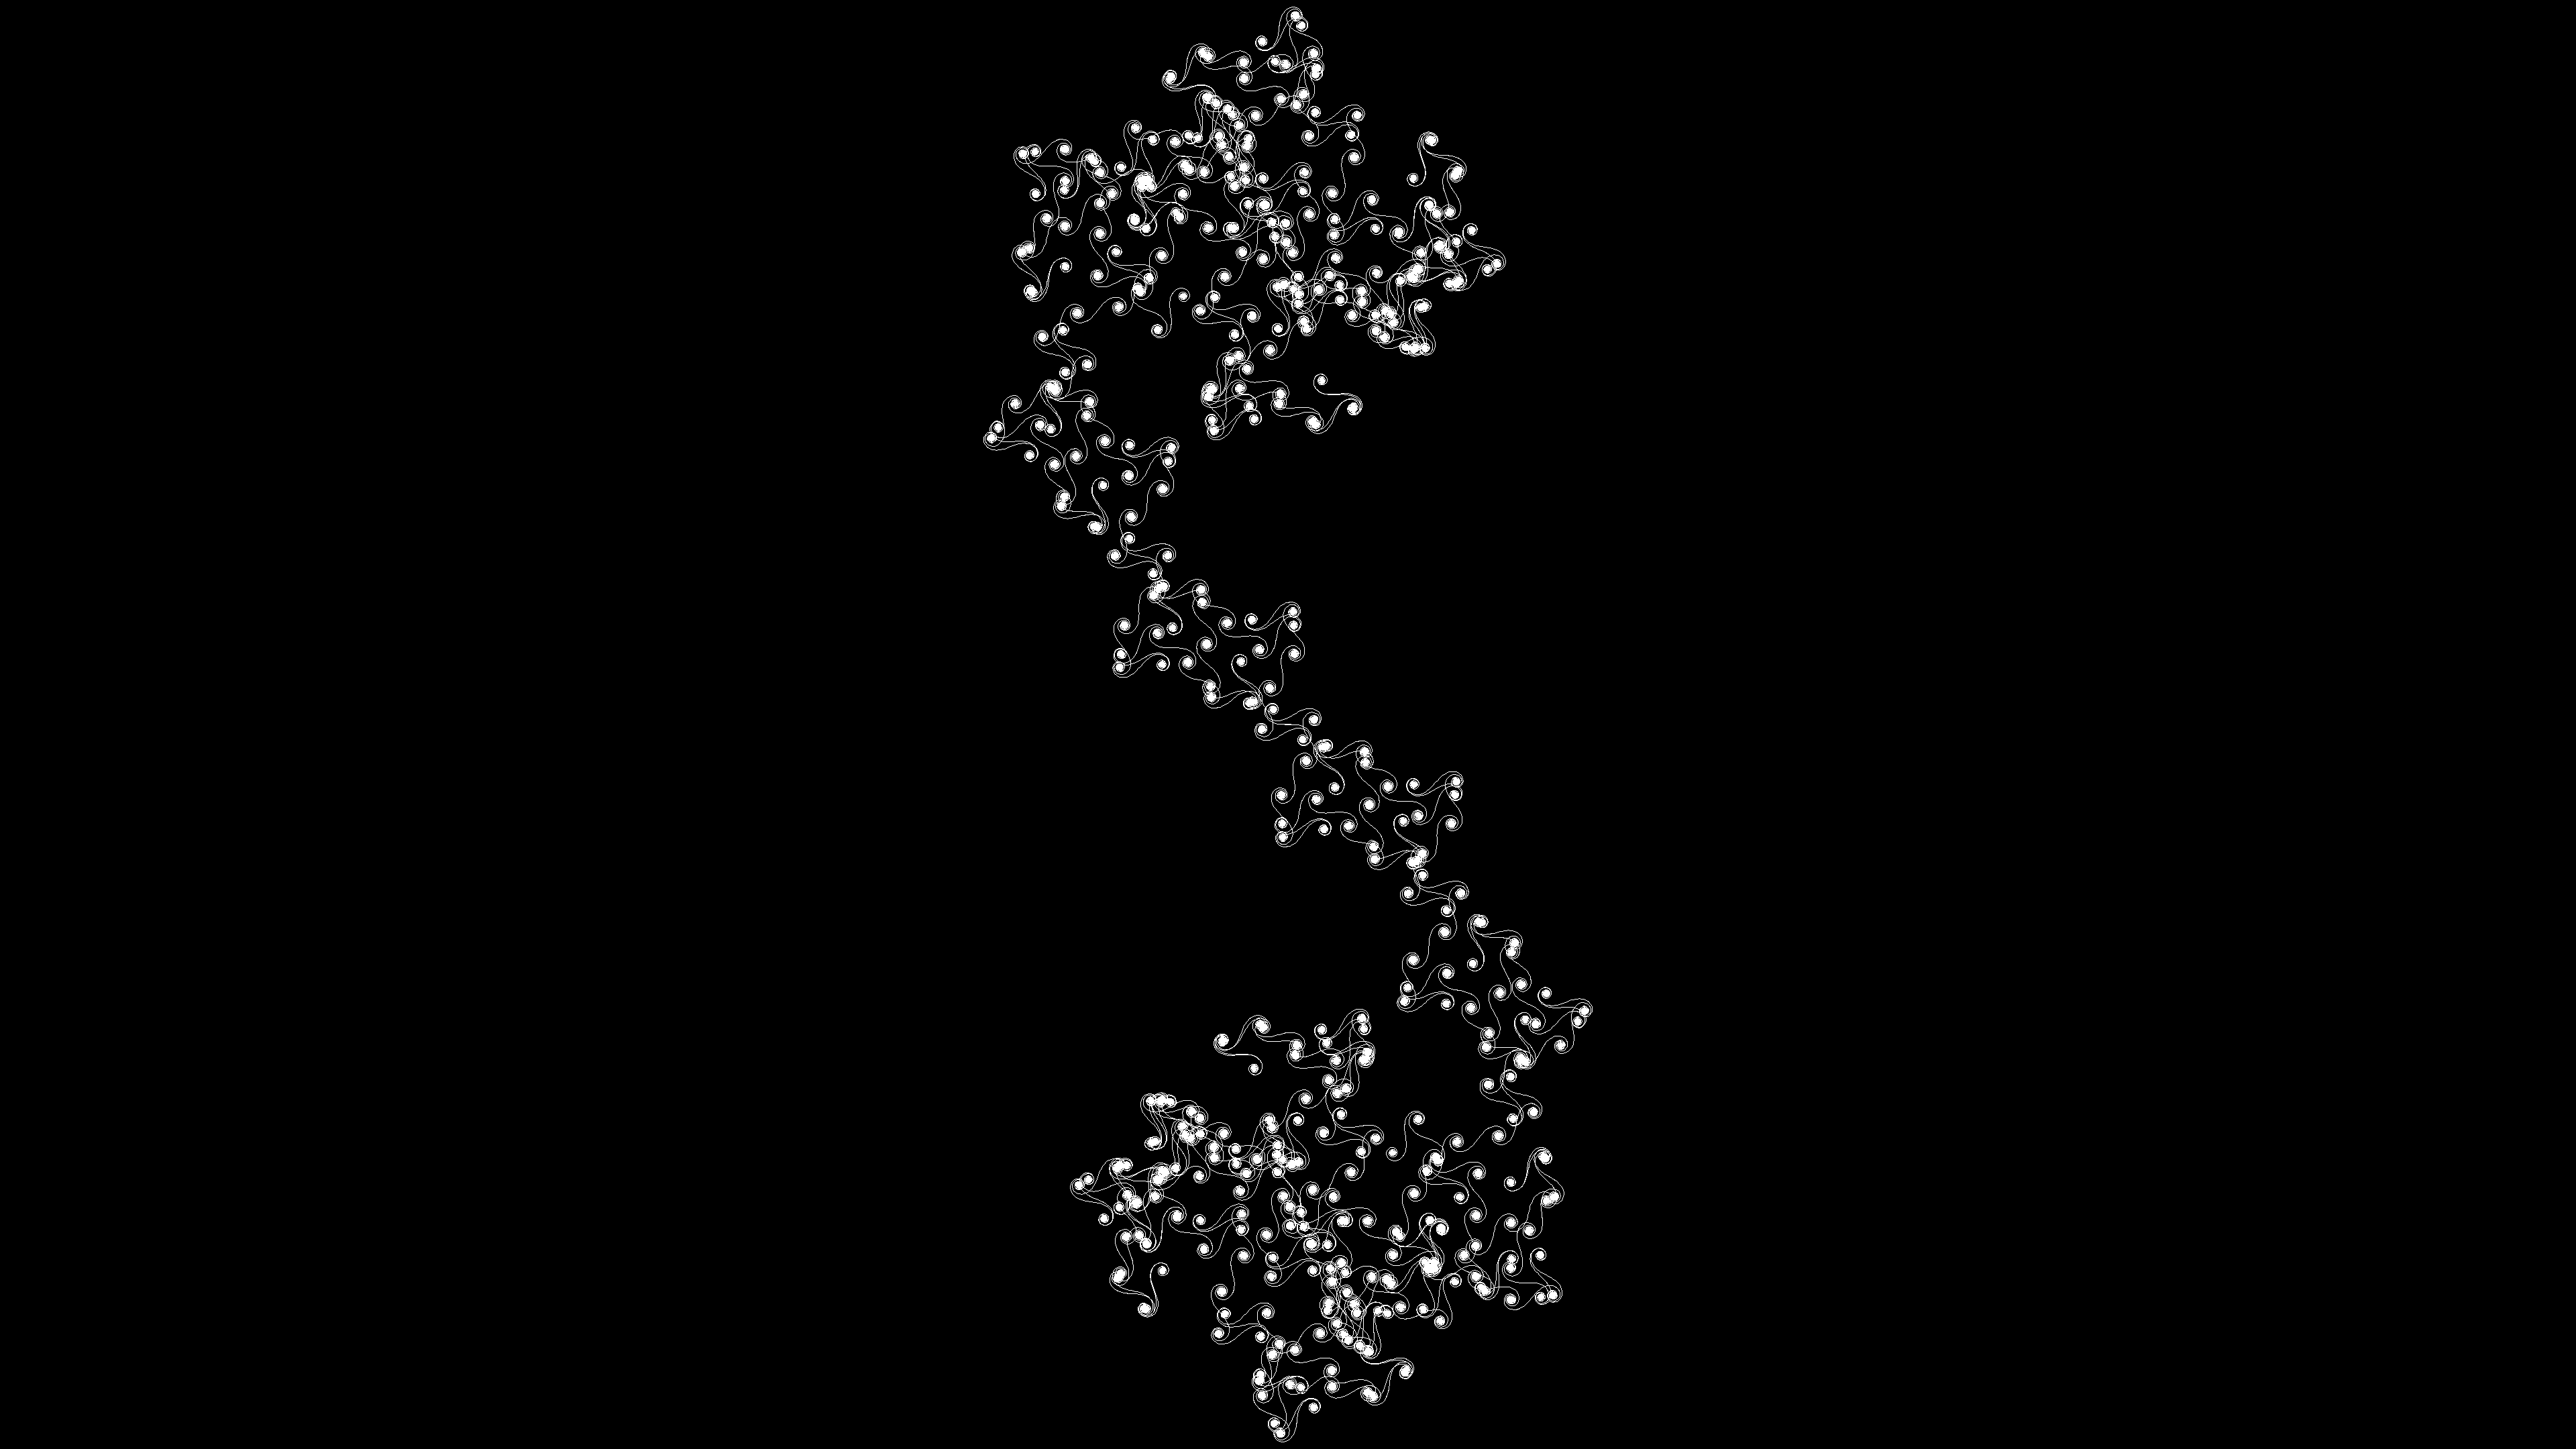
\includegraphics[width=\linewidth]{./stepsplusoneimages/0000000087.png}
    \caption{tf p=499 q=199686 theta=000 89961239.png}
  \end{subfigure}
  \begin{subfigure}[t]{0.48\textwidth}
    \centering
    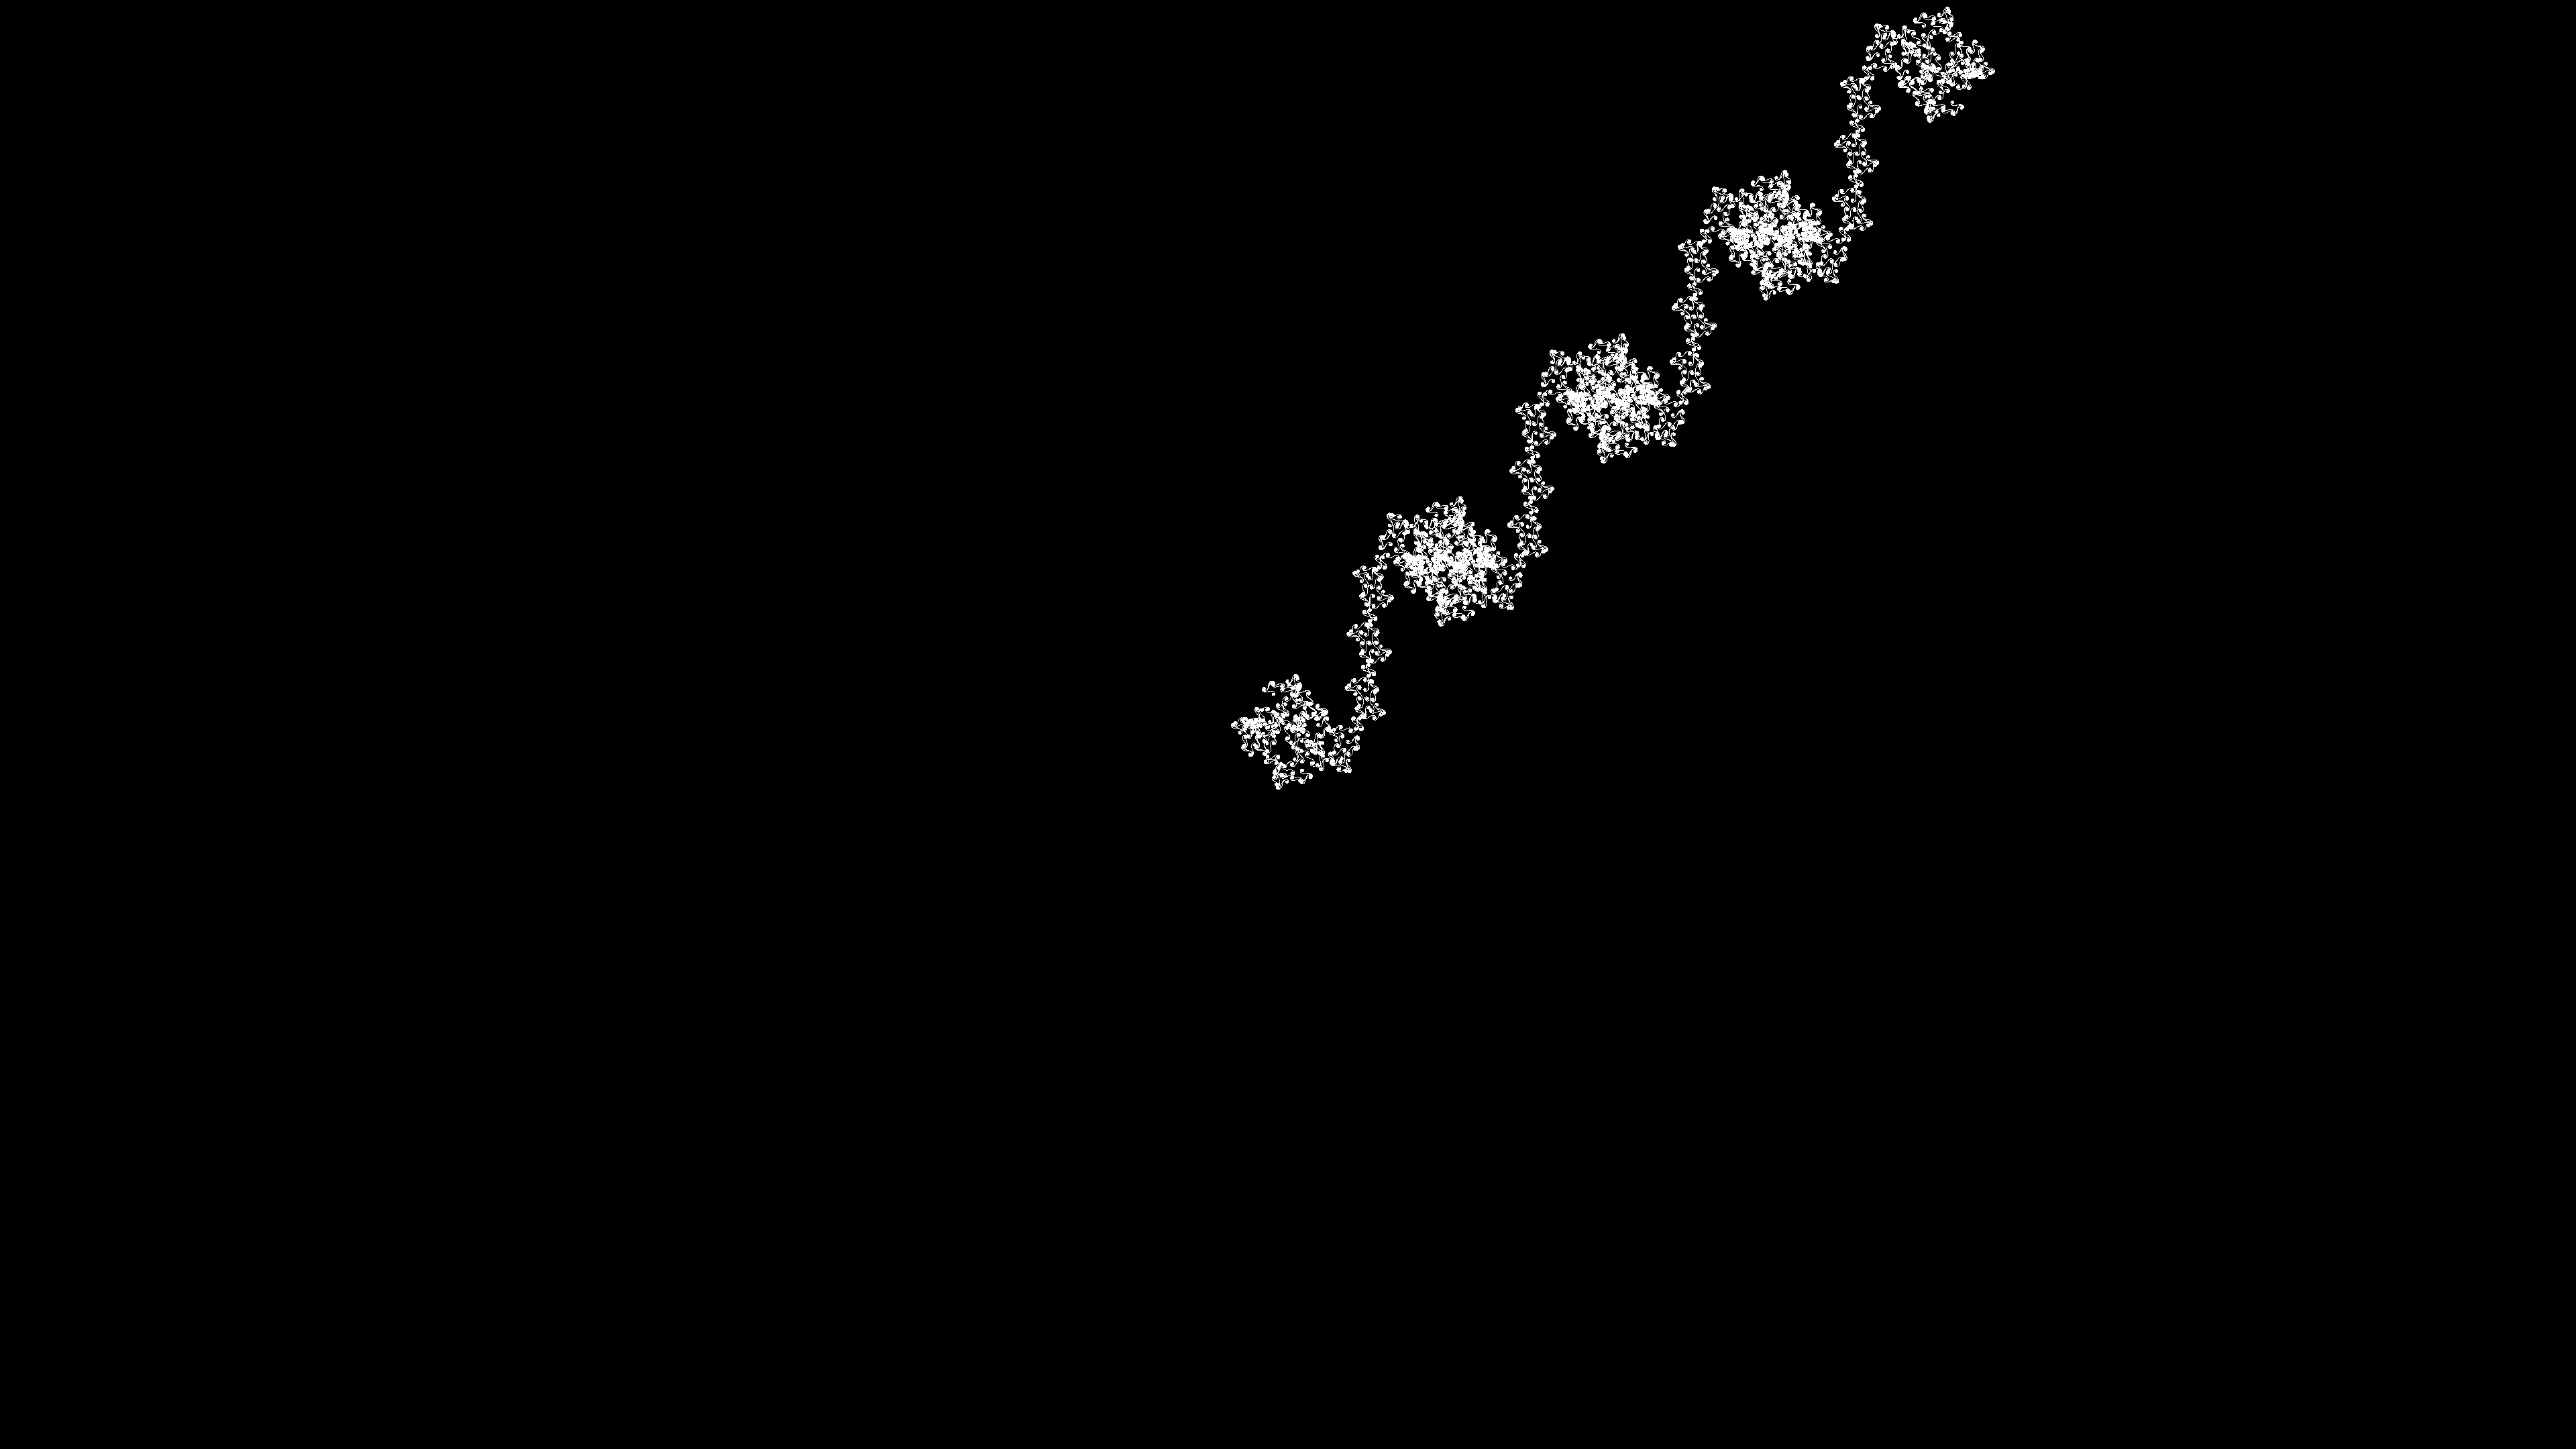
\includegraphics[width=\linewidth]{./stepsplusoneimages/0000000088.png}
    \caption{tf p=499 q=200185 theta=000 89736993.png}
  \end{subfigure}
  \caption{n=086 s=400 s+1=401}
  \label{fig:n=086}
\end{figure}
\begin{figure}[H]
  \centering
  \begin{subfigure}[t]{0.48\textwidth}
    \centering
    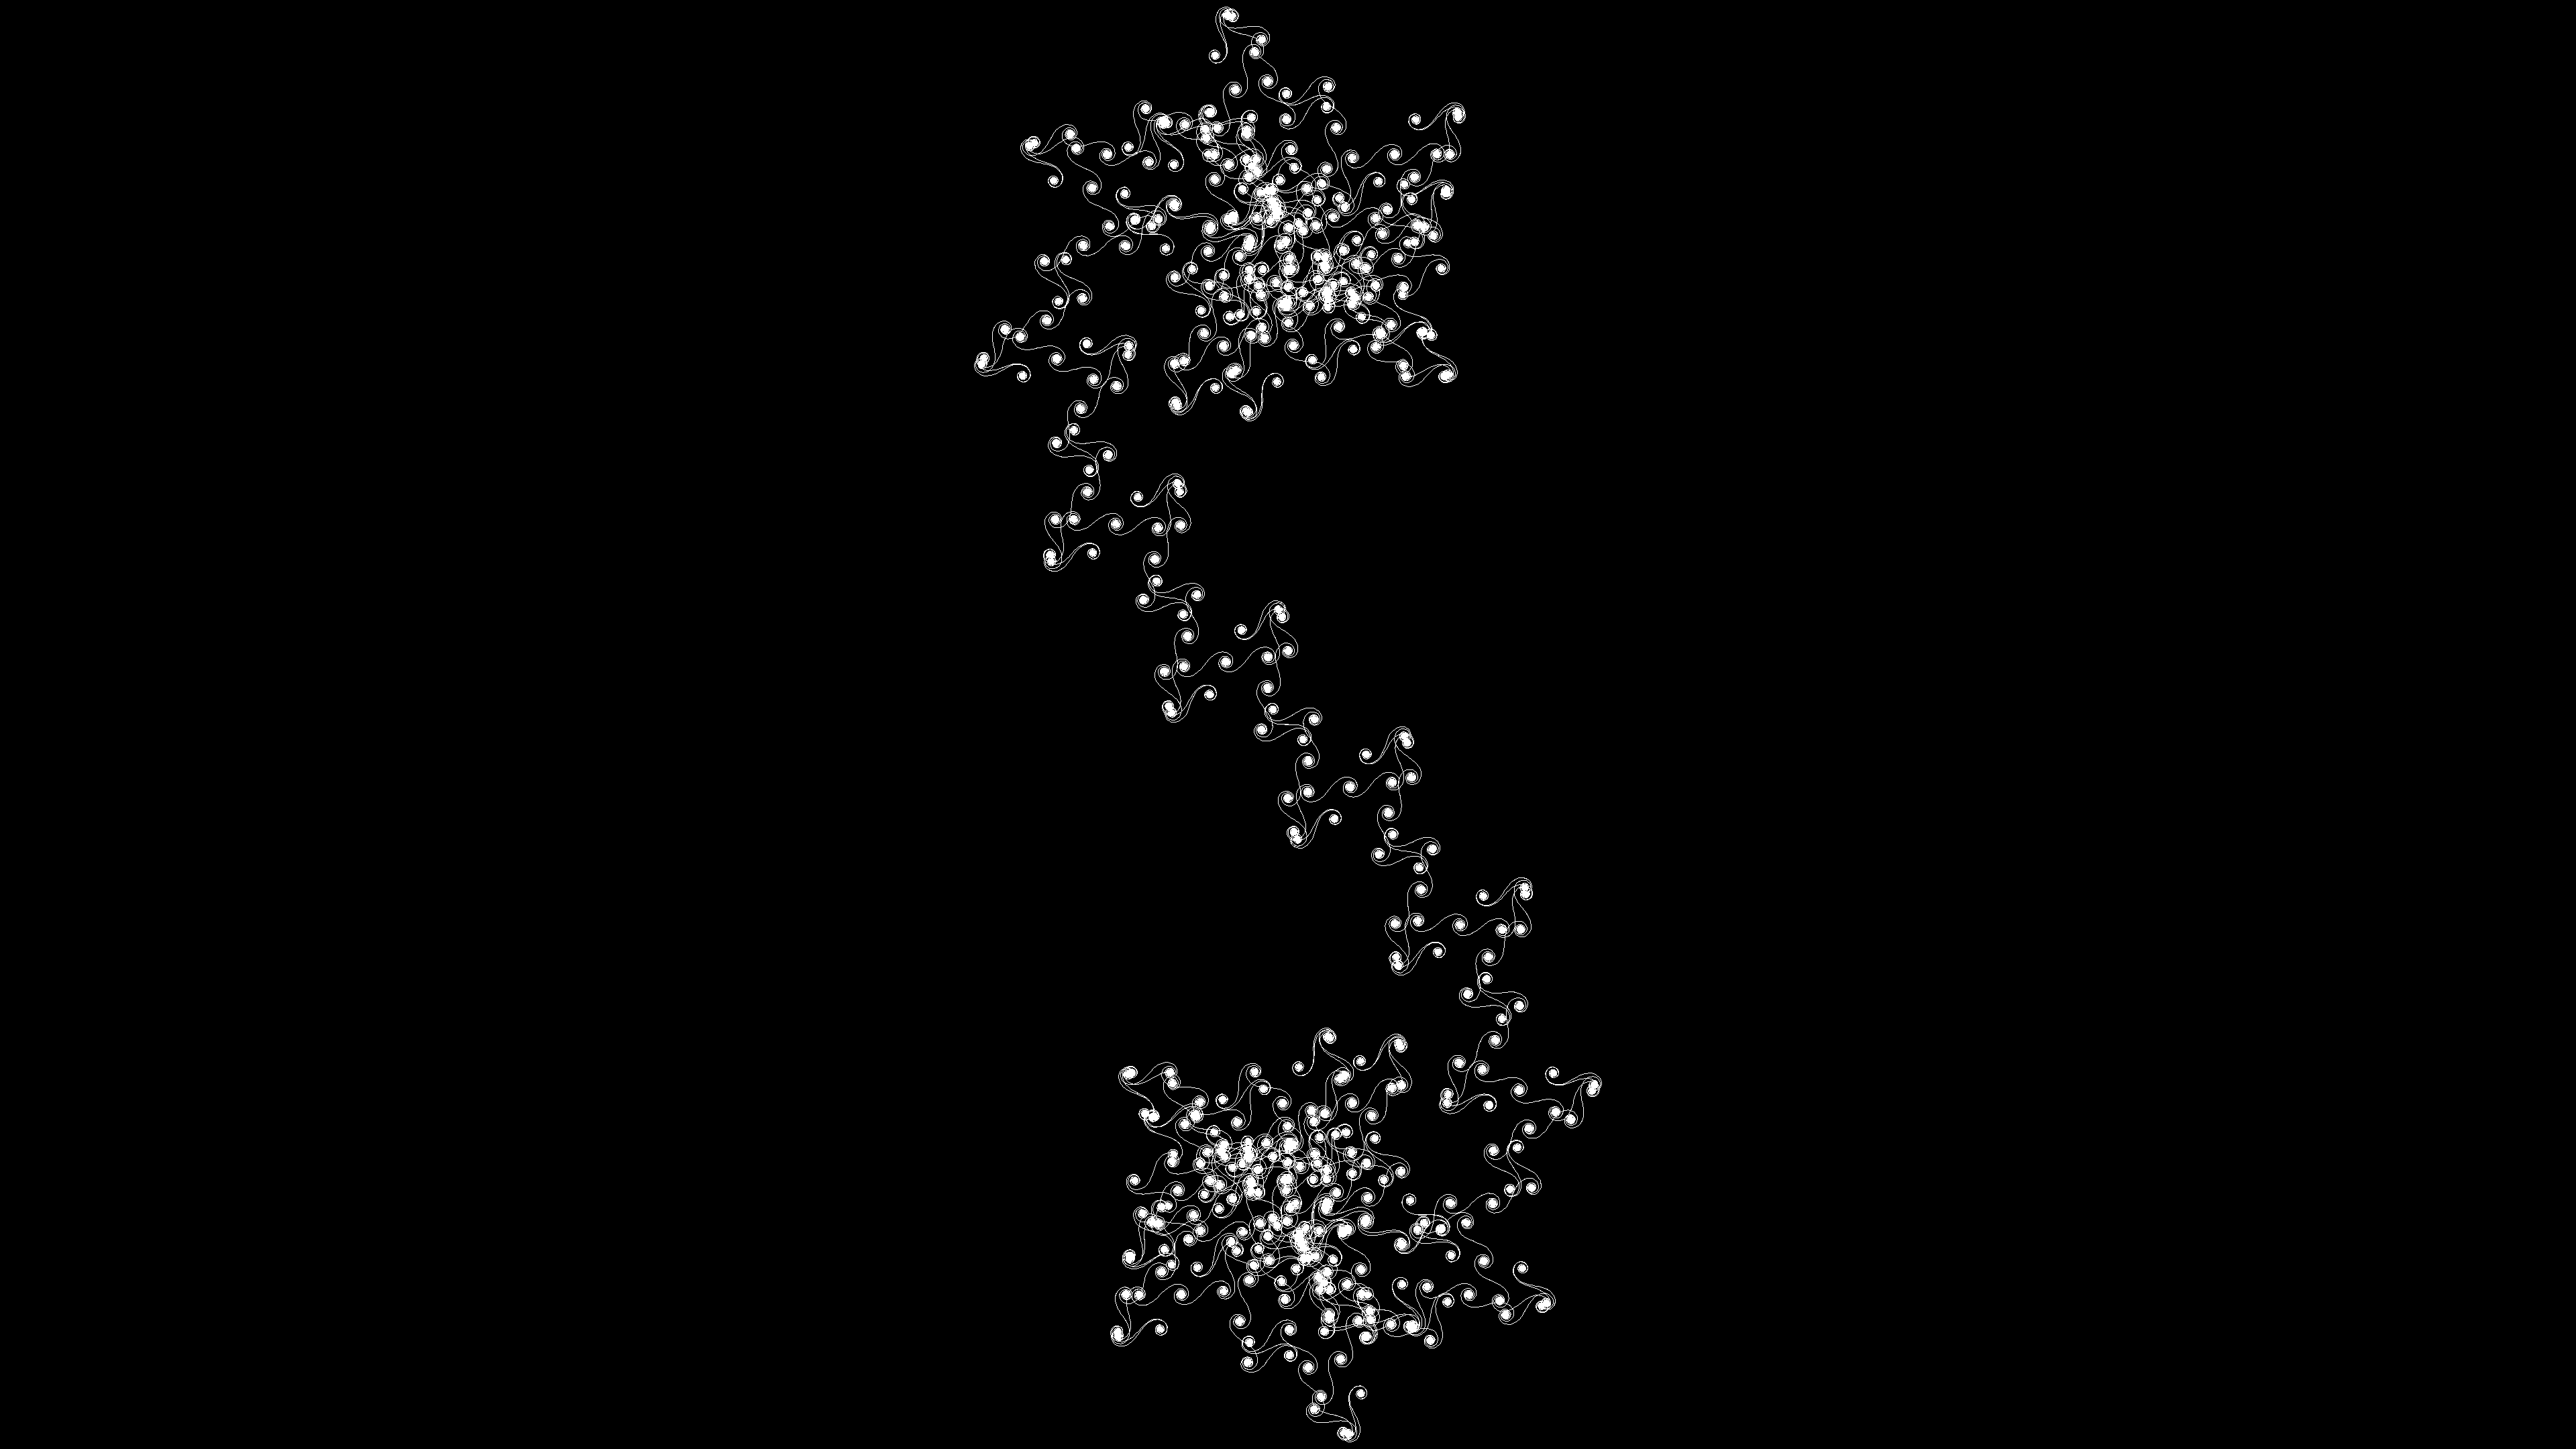
\includegraphics[width=\linewidth]{./stepsplusoneimages/0000000089.png}
    \caption{tf p=499 q=199688 theta=000 89960338.png}
  \end{subfigure}
  \begin{subfigure}[t]{0.48\textwidth}
    \centering
    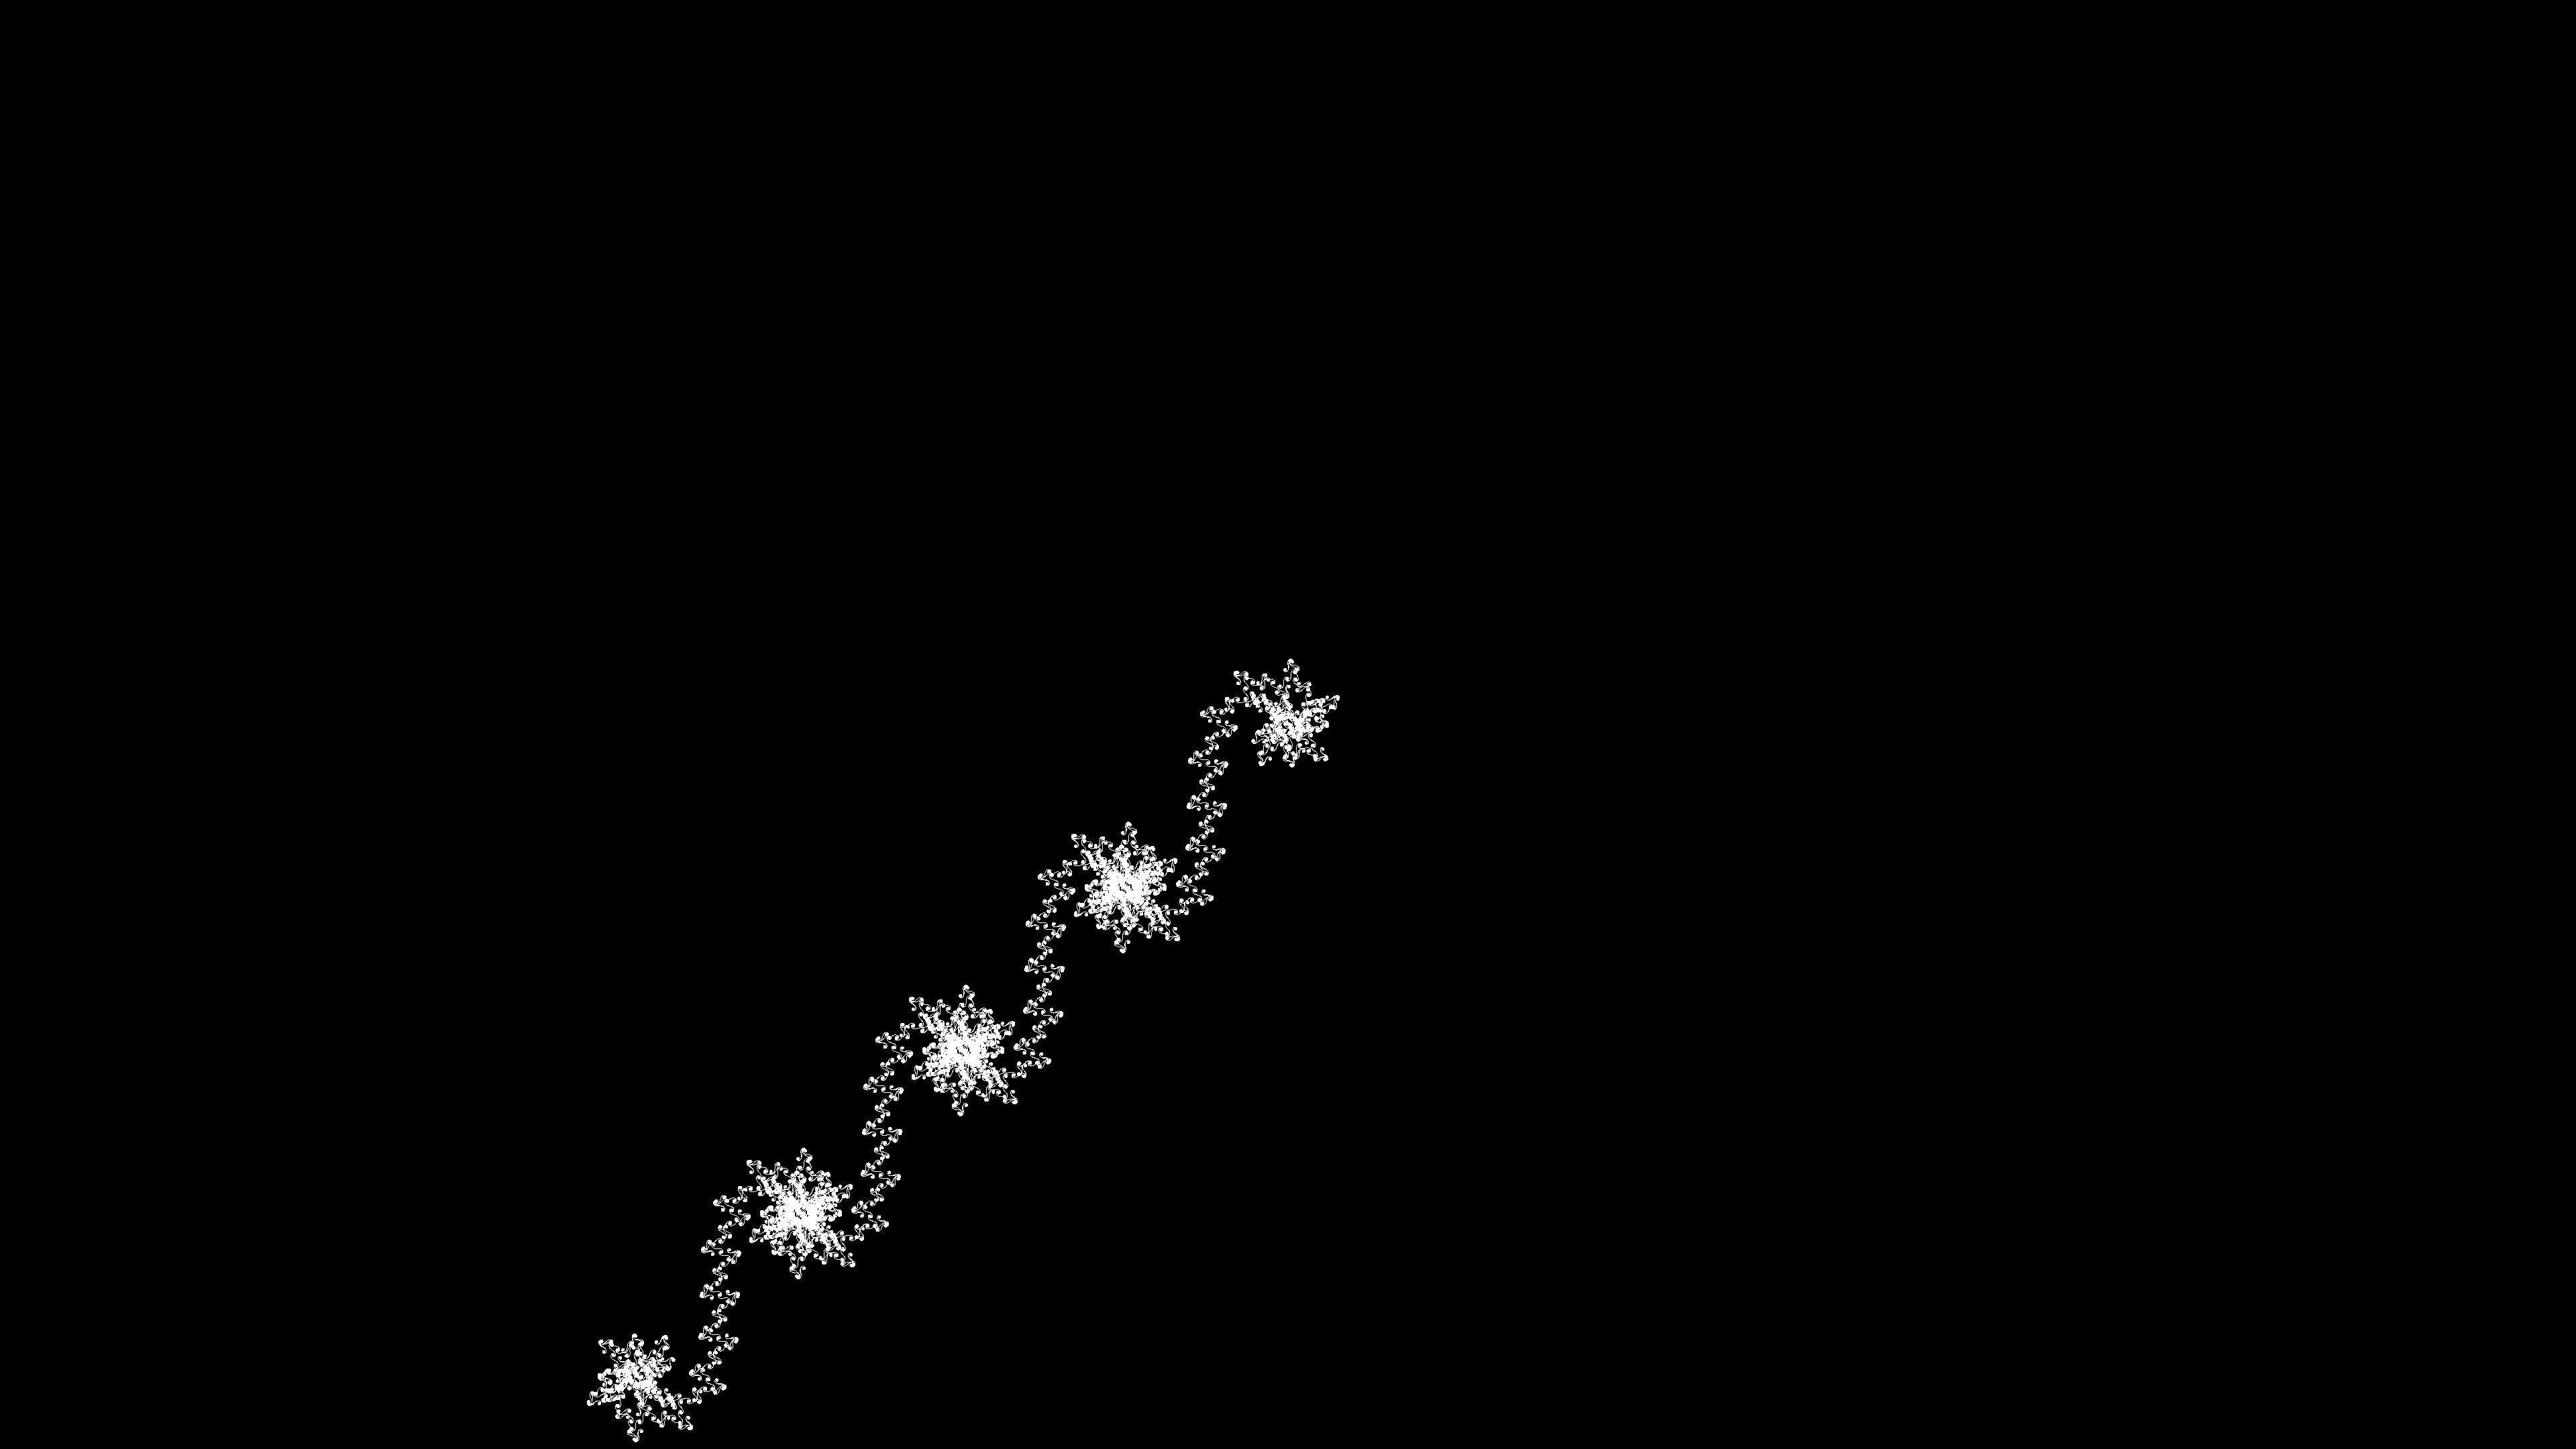
\includegraphics[width=\linewidth]{./stepsplusoneimages/0000000090.png}
    \caption{tf p=499 q=200187 theta=000 89736097.png}
  \end{subfigure}
  \caption{n=088 s=400 s+1=401}
  \label{fig:n=088}
\end{figure}
\begin{figure}[H]
  \centering
  \begin{subfigure}[t]{0.48\textwidth}
    \centering
    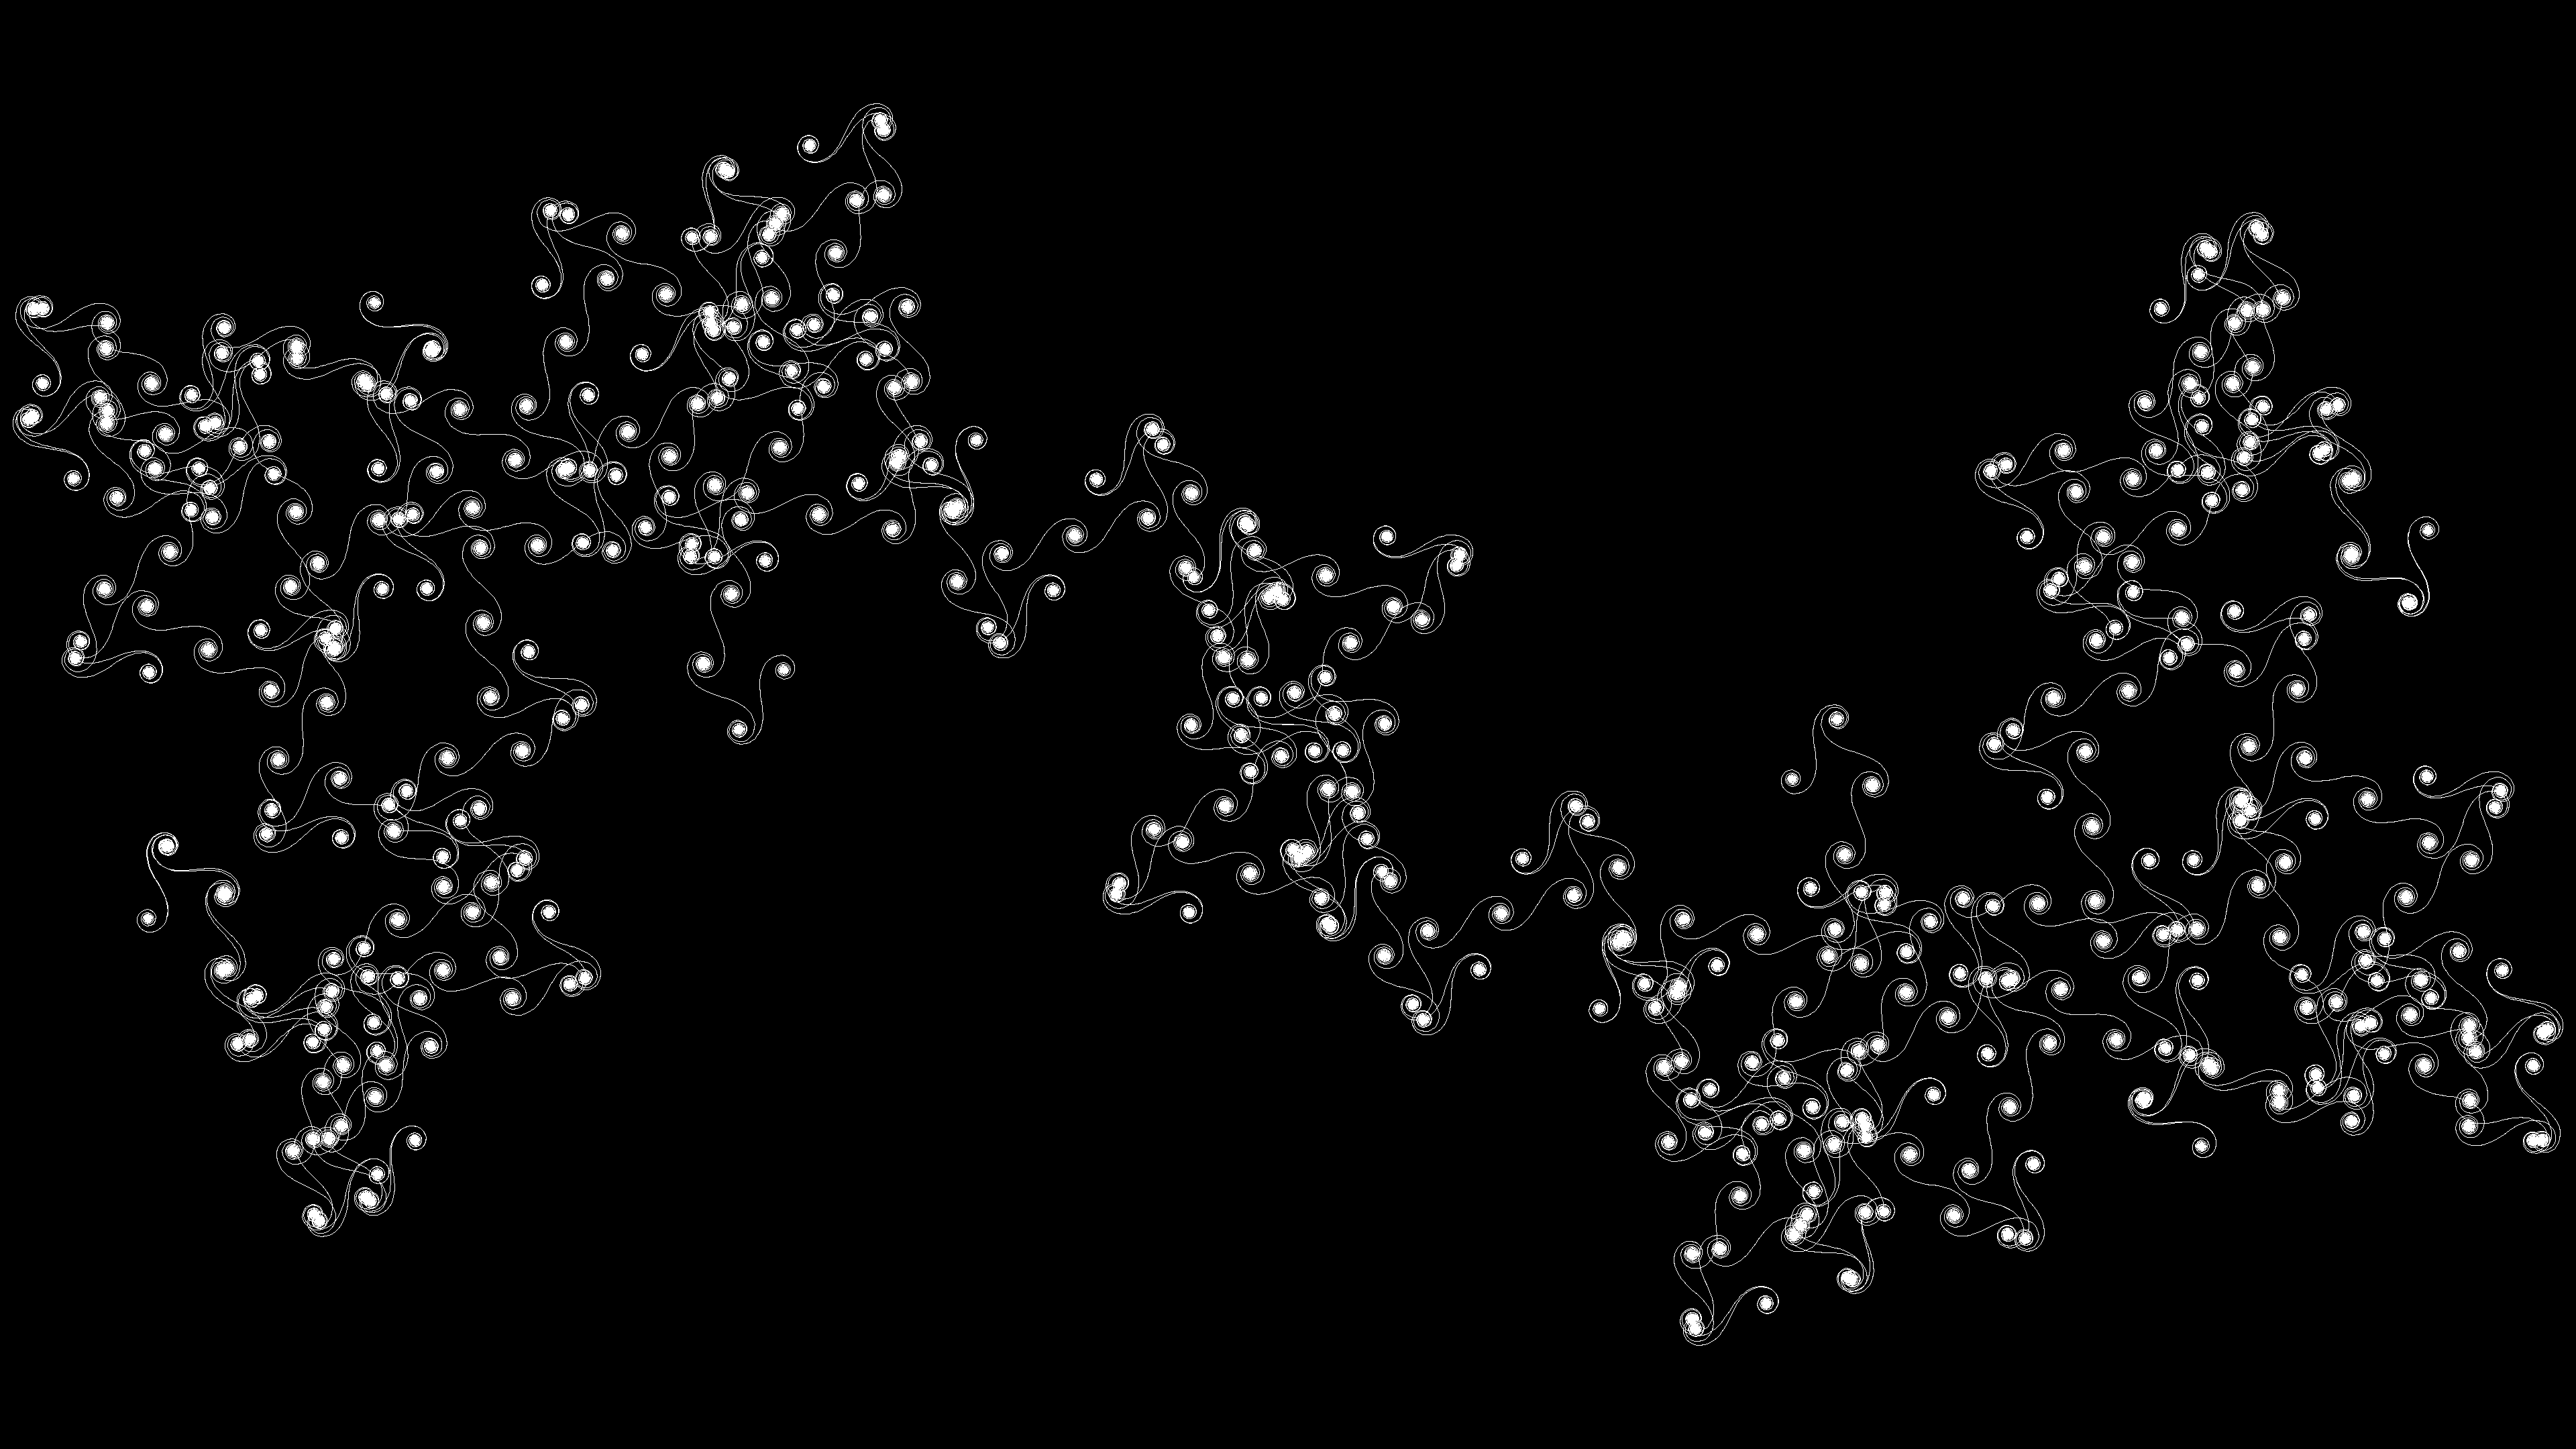
\includegraphics[width=\linewidth]{./stepsplusoneimages/0000000091.png}
    \caption{tf p=499 q=199690 theta=000 89959437.png}
  \end{subfigure}
  \begin{subfigure}[t]{0.48\textwidth}
    \centering
    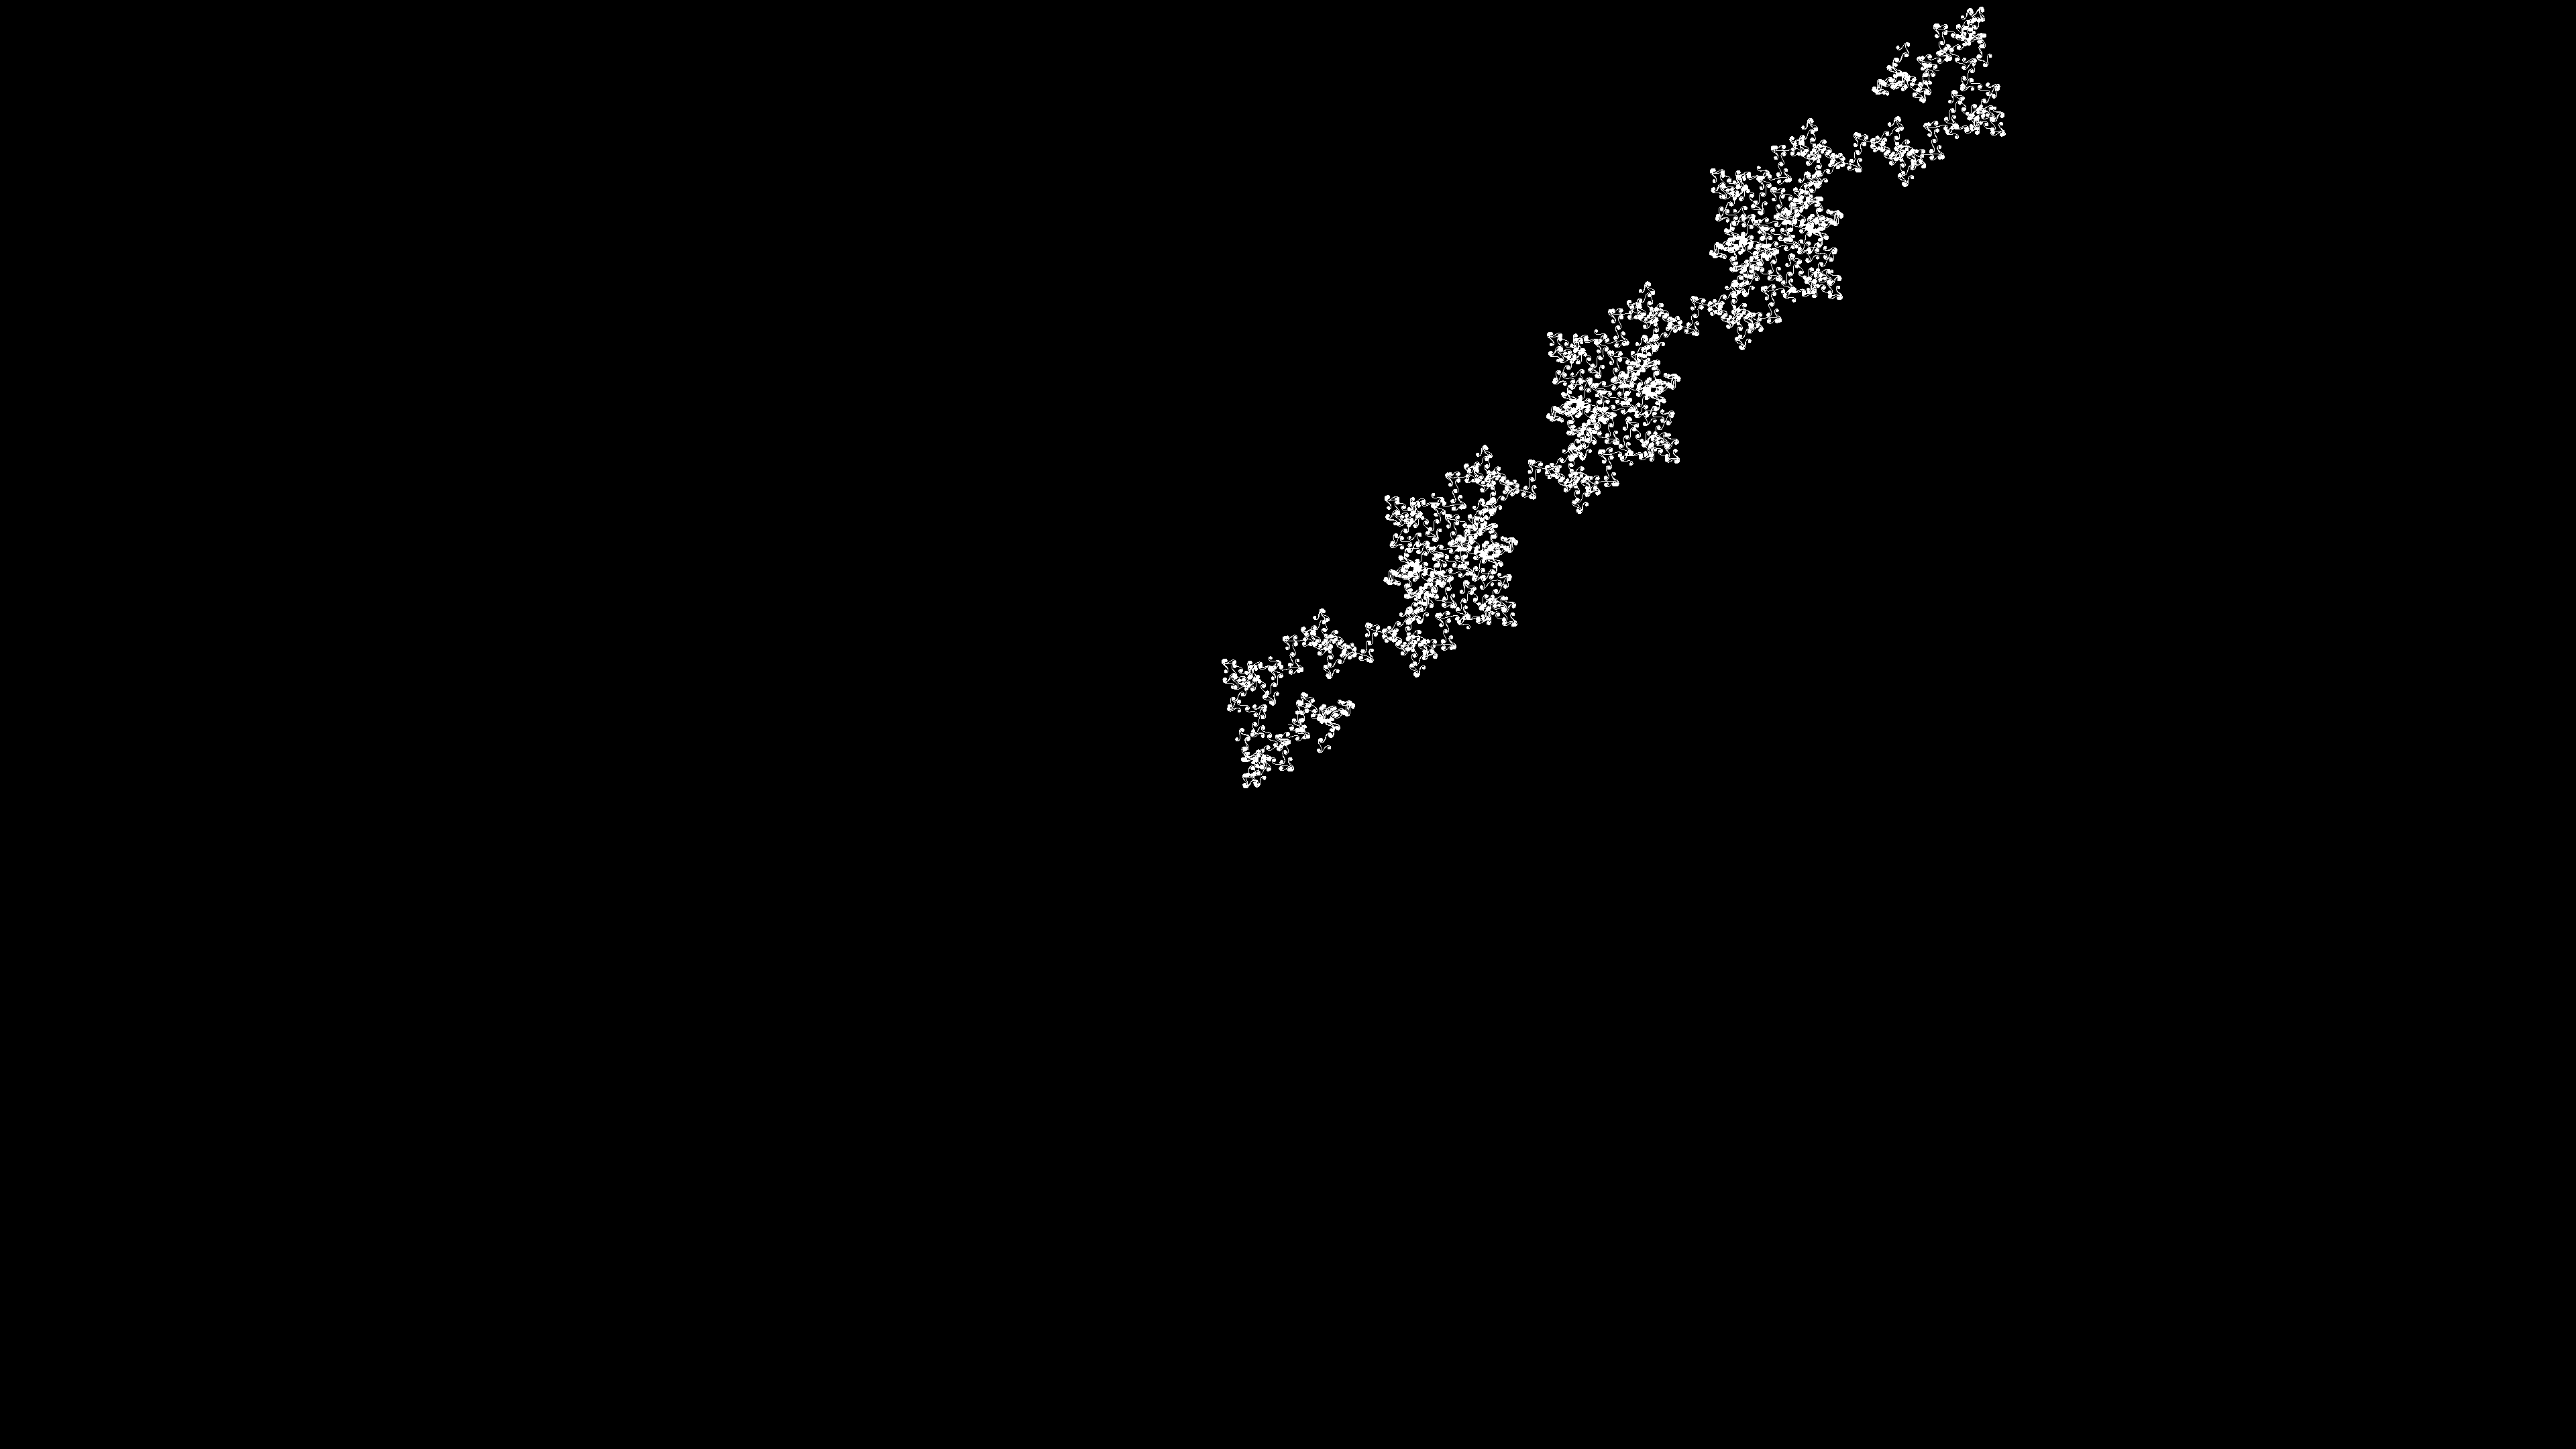
\includegraphics[width=\linewidth]{./stepsplusoneimages/0000000092.png}
    \caption{tf p=499 q=200189 theta=000 89735200.png}
  \end{subfigure}
  \caption{n=090 s=400 s+1=401}
  \label{fig:n=090}
\end{figure}
\begin{figure}[H]
  \centering
  \begin{subfigure}[t]{0.48\textwidth}
    \centering
    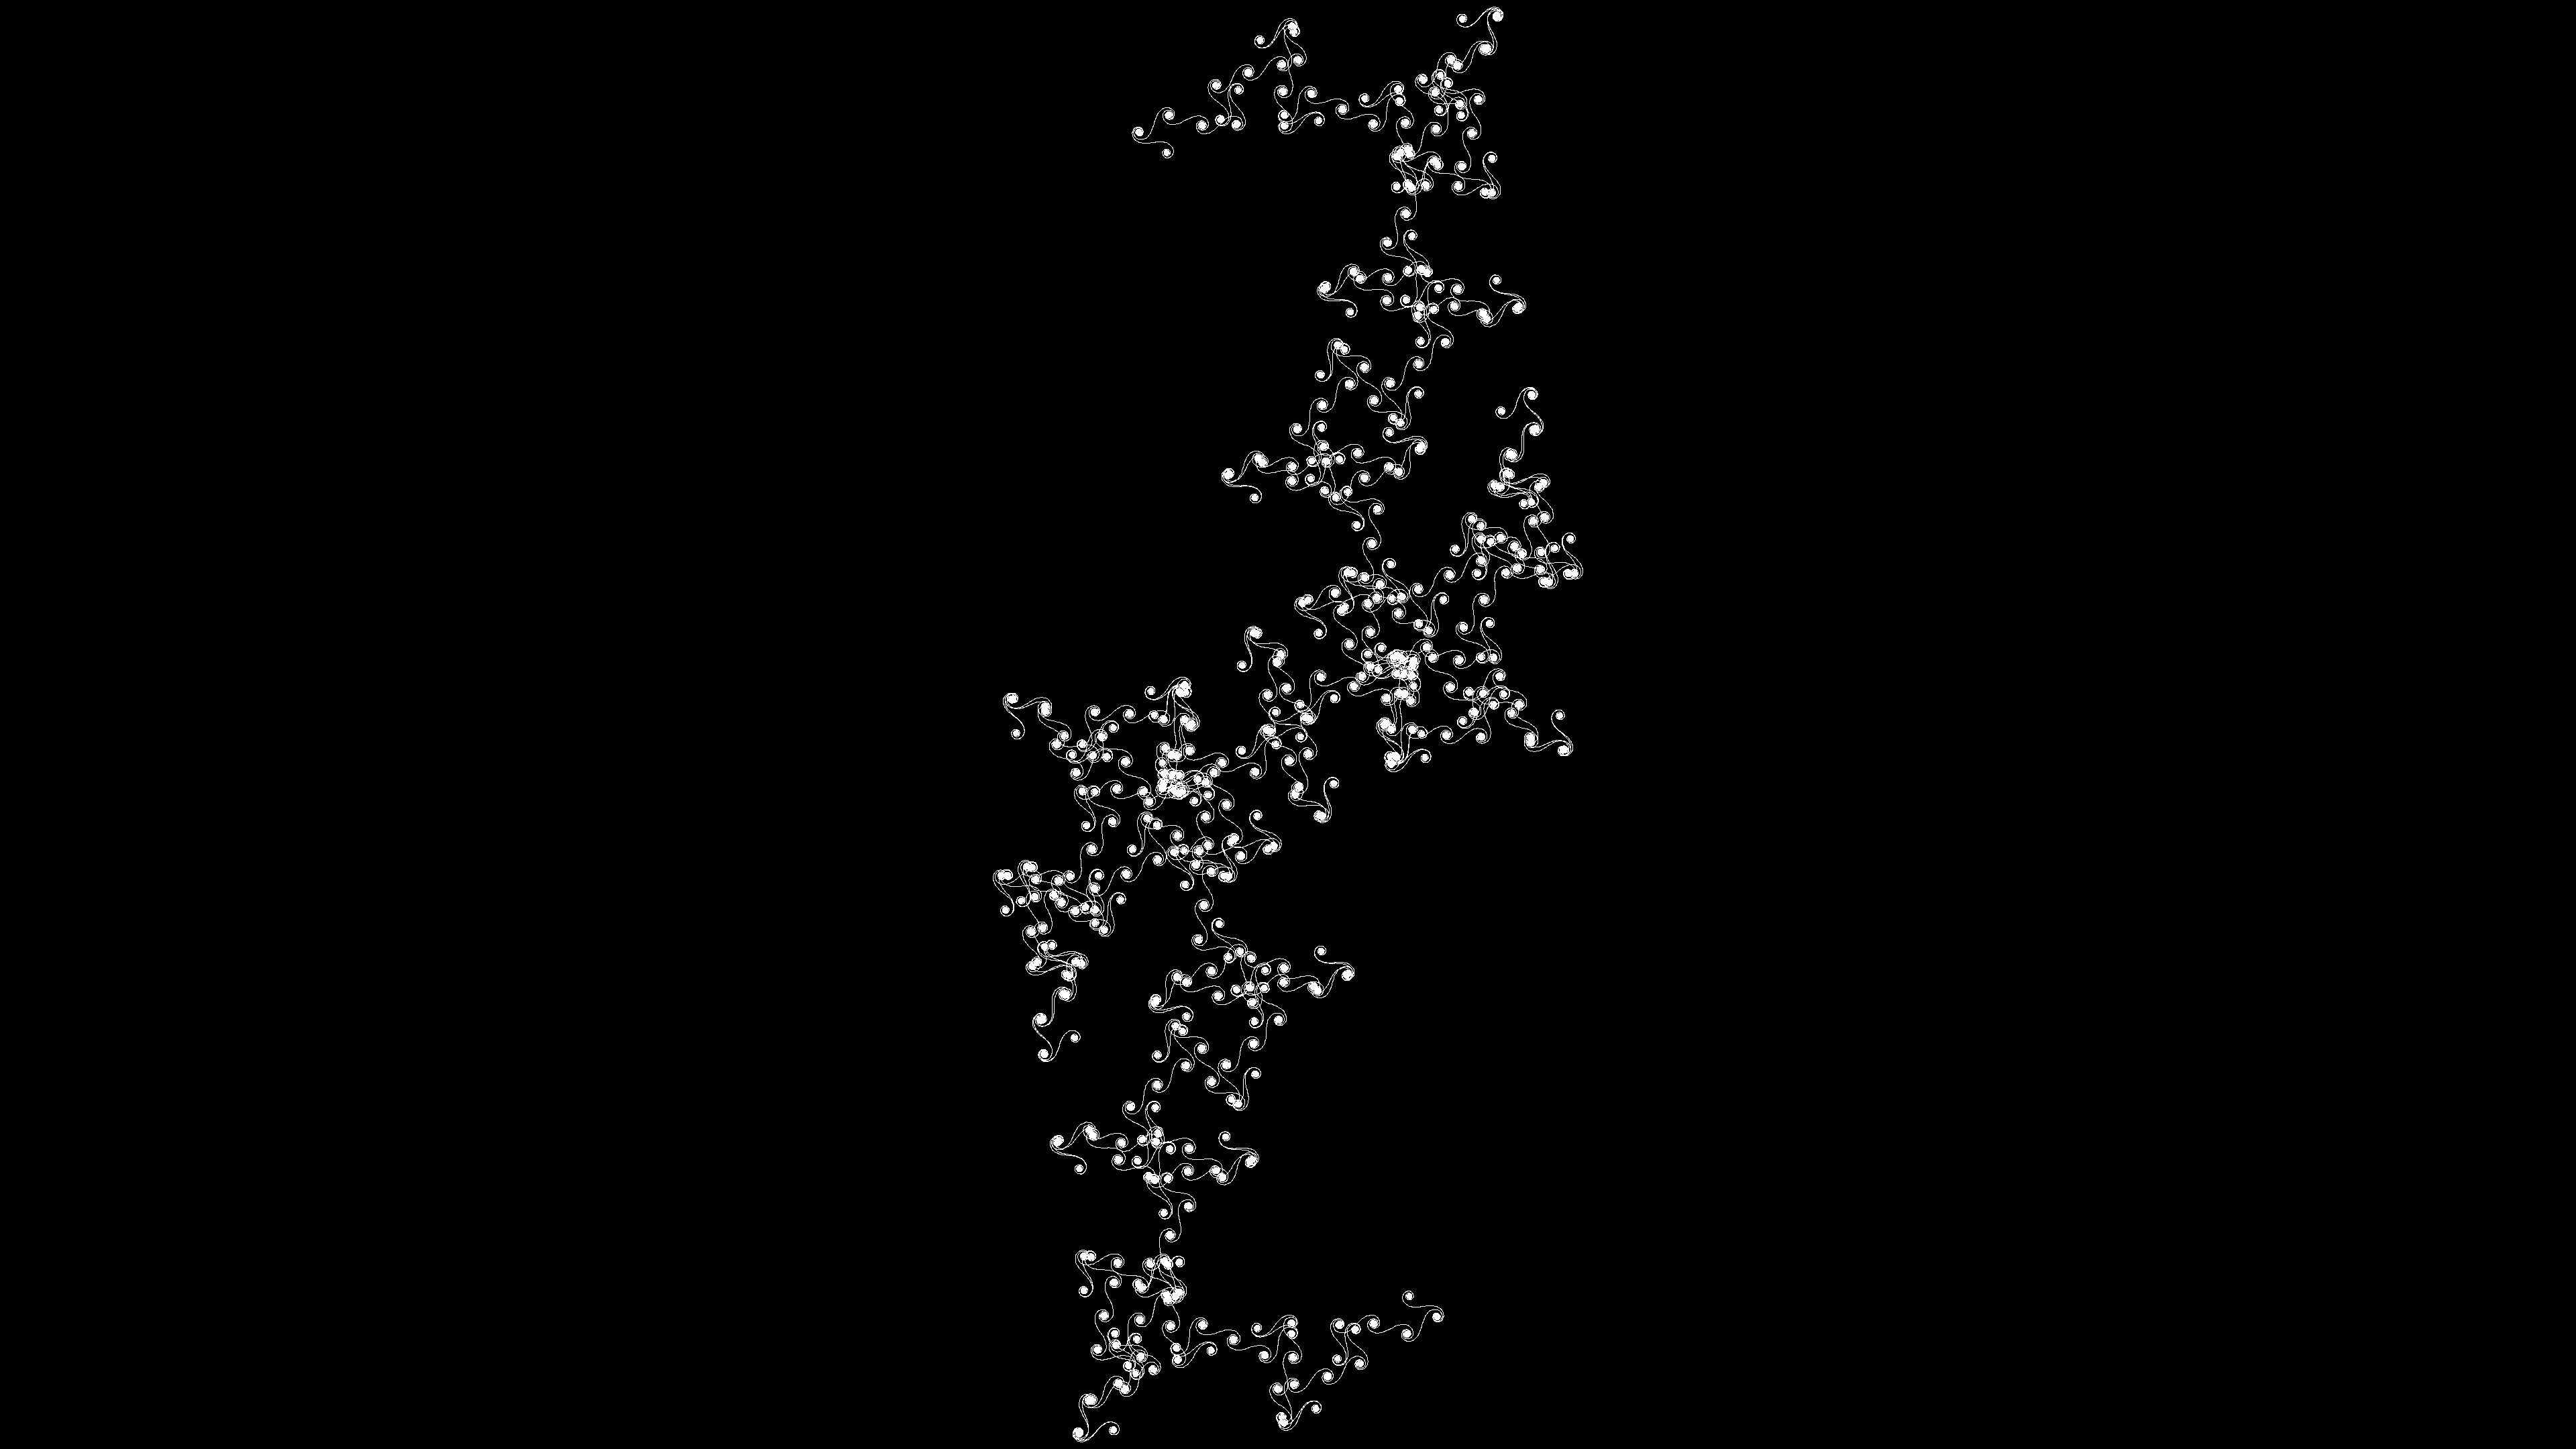
\includegraphics[width=\linewidth]{./stepsplusoneimages/0000000093.png}
    \caption{tf p=499 q=199692 theta=000 89958536.png}
  \end{subfigure}
  \begin{subfigure}[t]{0.48\textwidth}
    \centering
    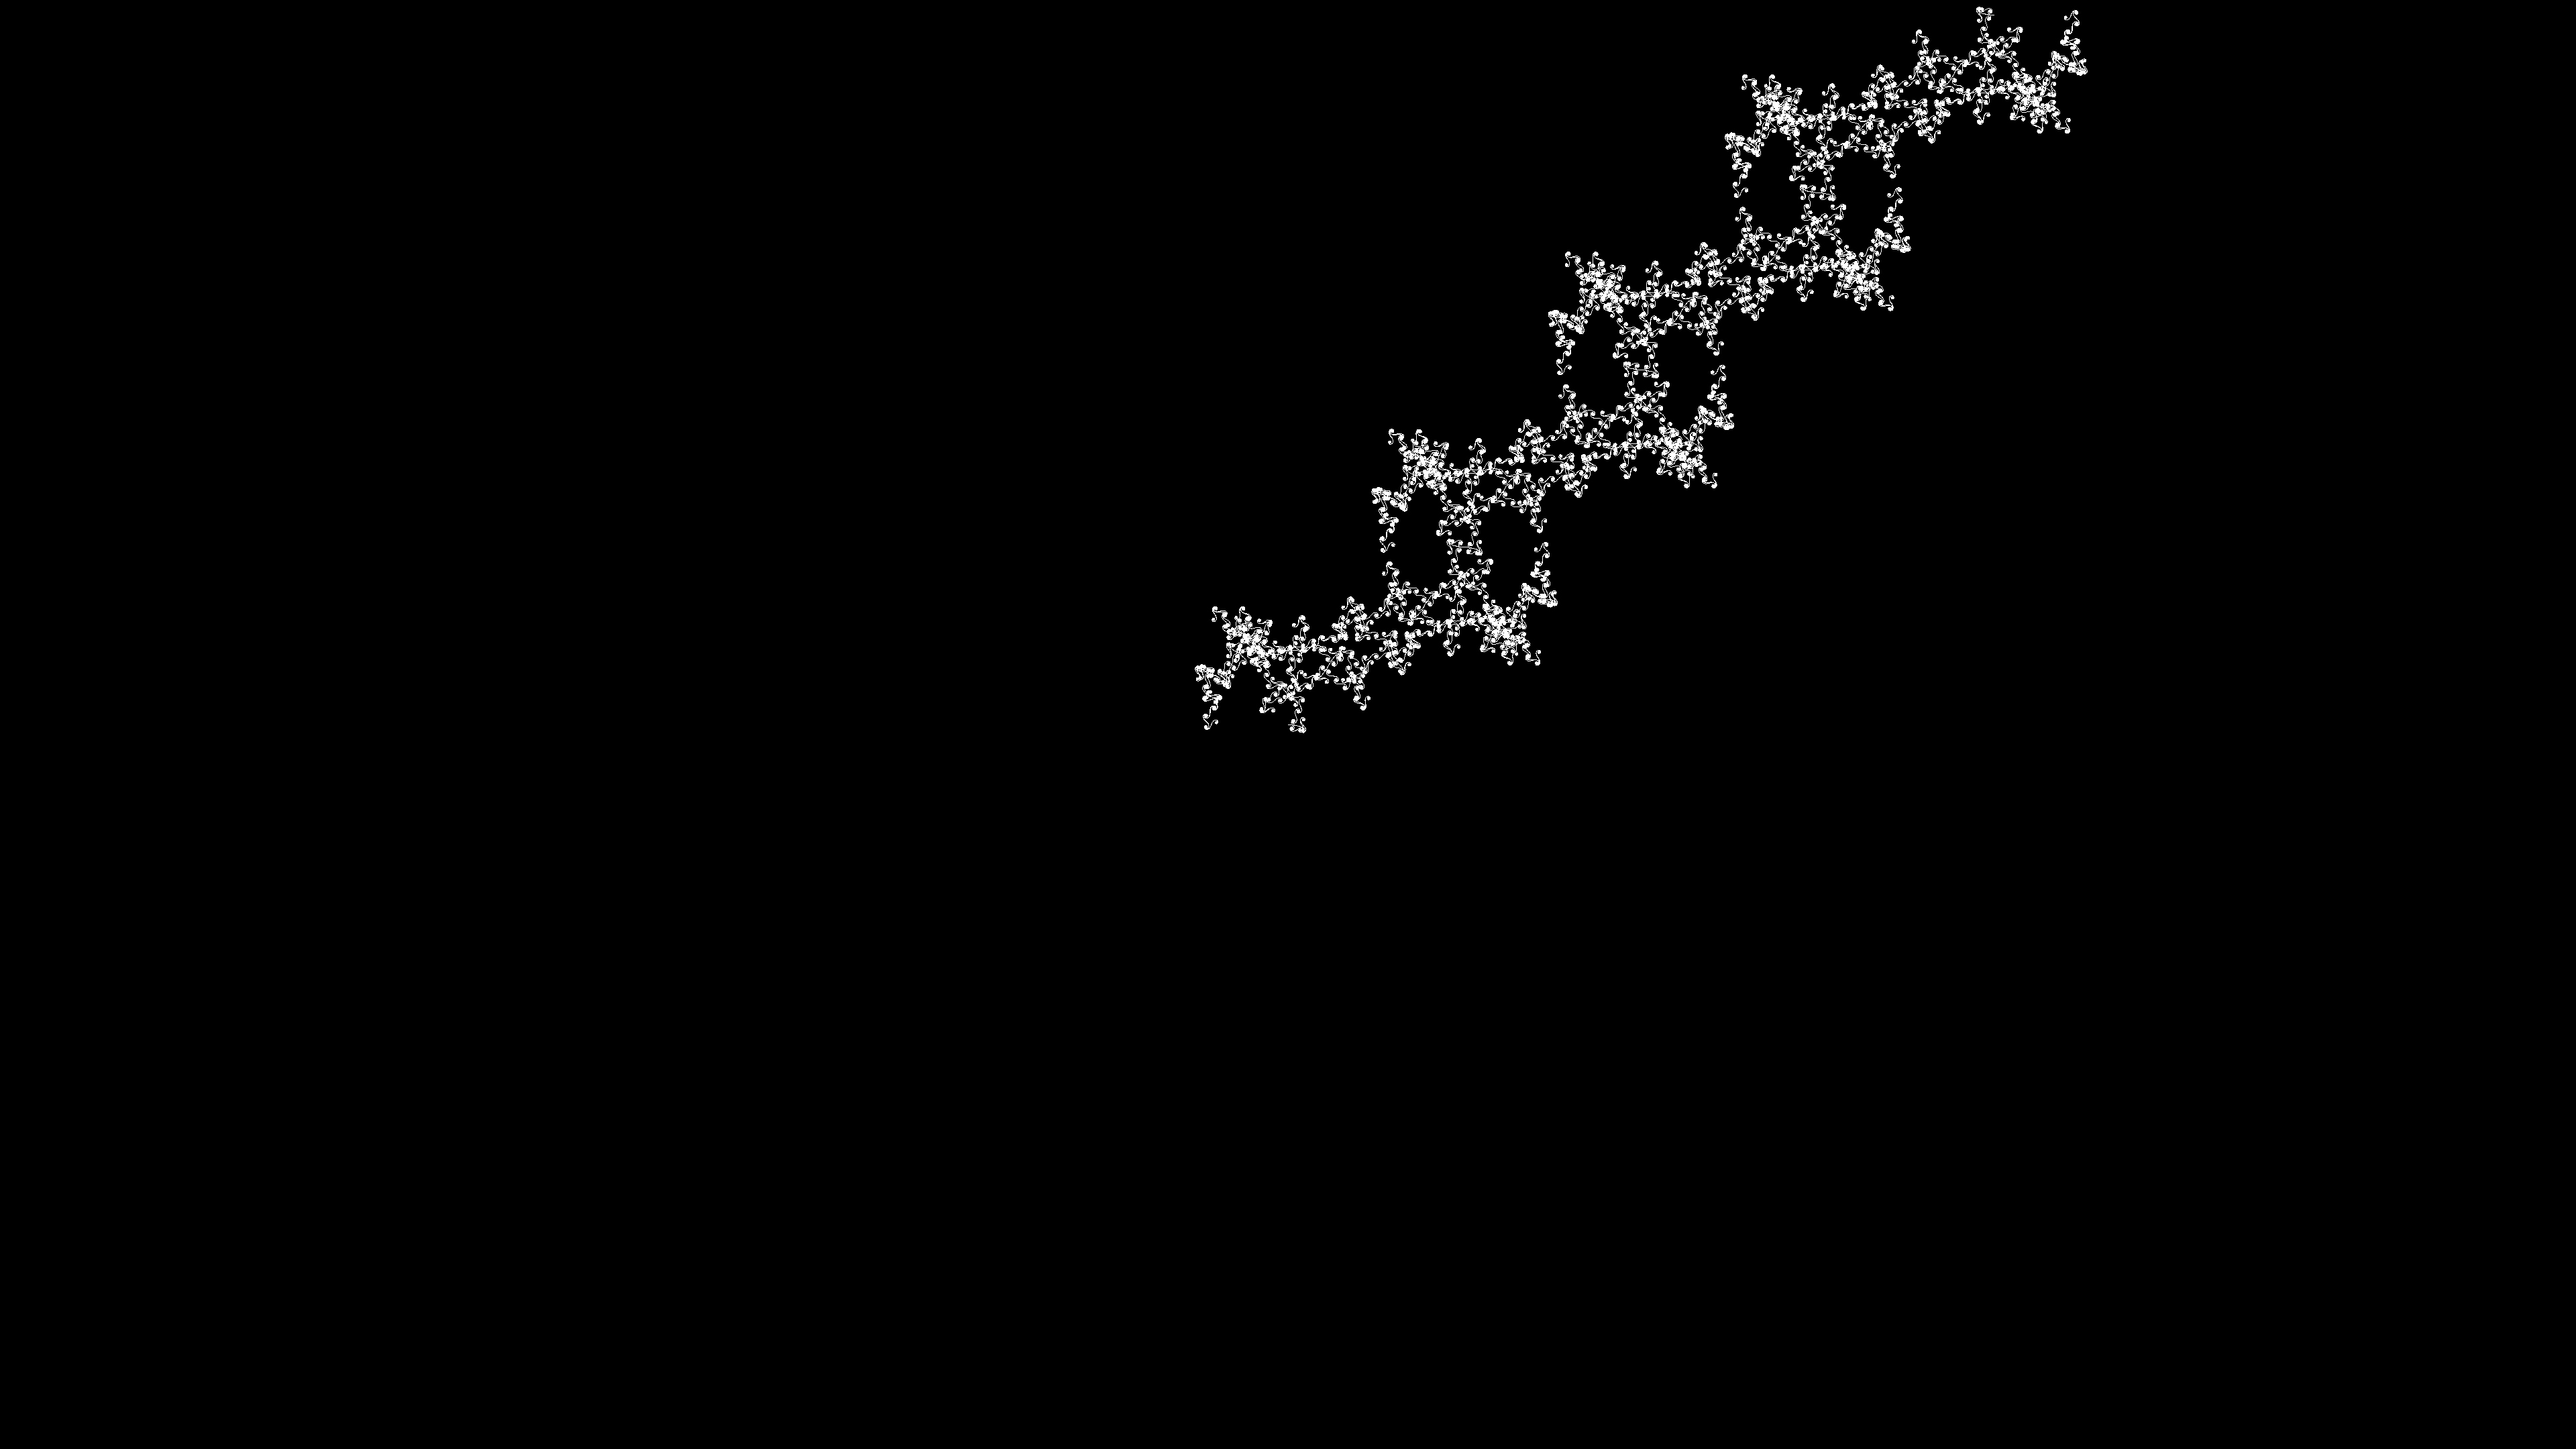
\includegraphics[width=\linewidth]{./stepsplusoneimages/0000000094.png}
    \caption{tf p=499 q=200191 theta=000 89734304.png}
  \end{subfigure}
  \caption{n=092 s=400 s+1=401}
  \label{fig:n=092}
\end{figure}
\begin{figure}[H]
  \centering
  \begin{subfigure}[t]{0.48\textwidth}
    \centering
    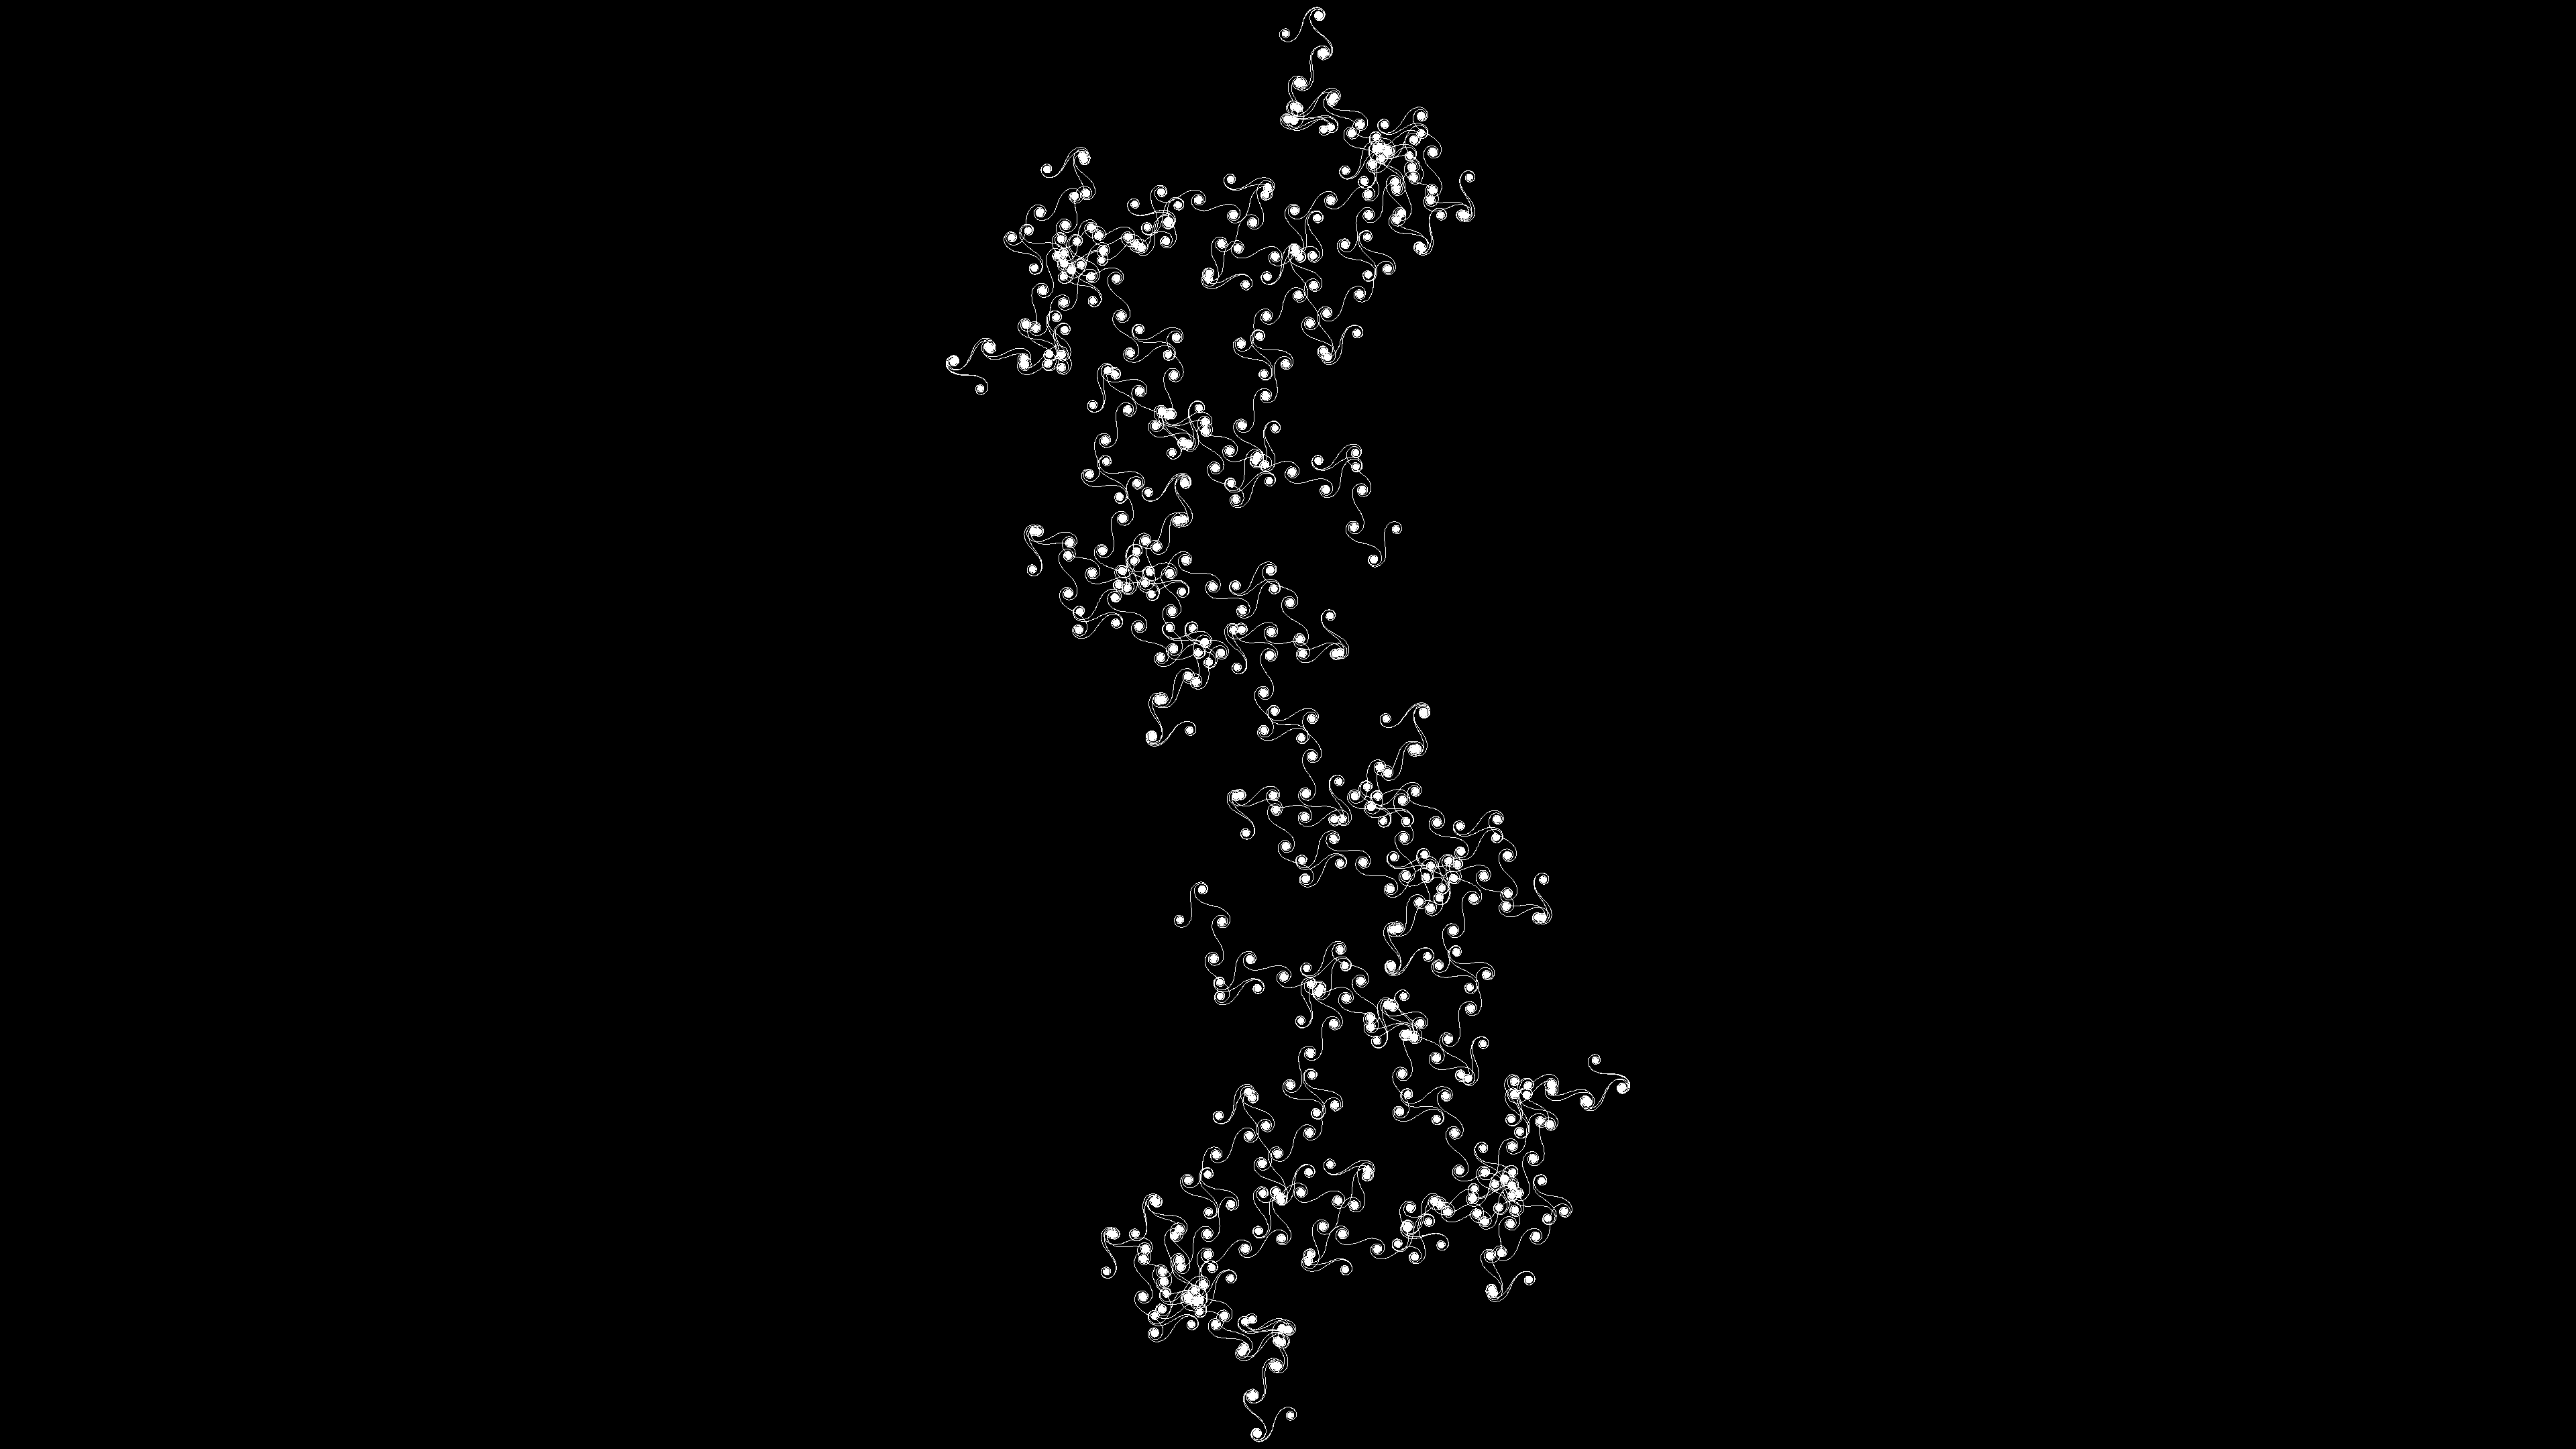
\includegraphics[width=\linewidth]{./stepsplusoneimages/0000000095.png}
    \caption{tf p=499 q=199694 theta=000 89957635.png}
  \end{subfigure}
  \begin{subfigure}[t]{0.48\textwidth}
    \centering
    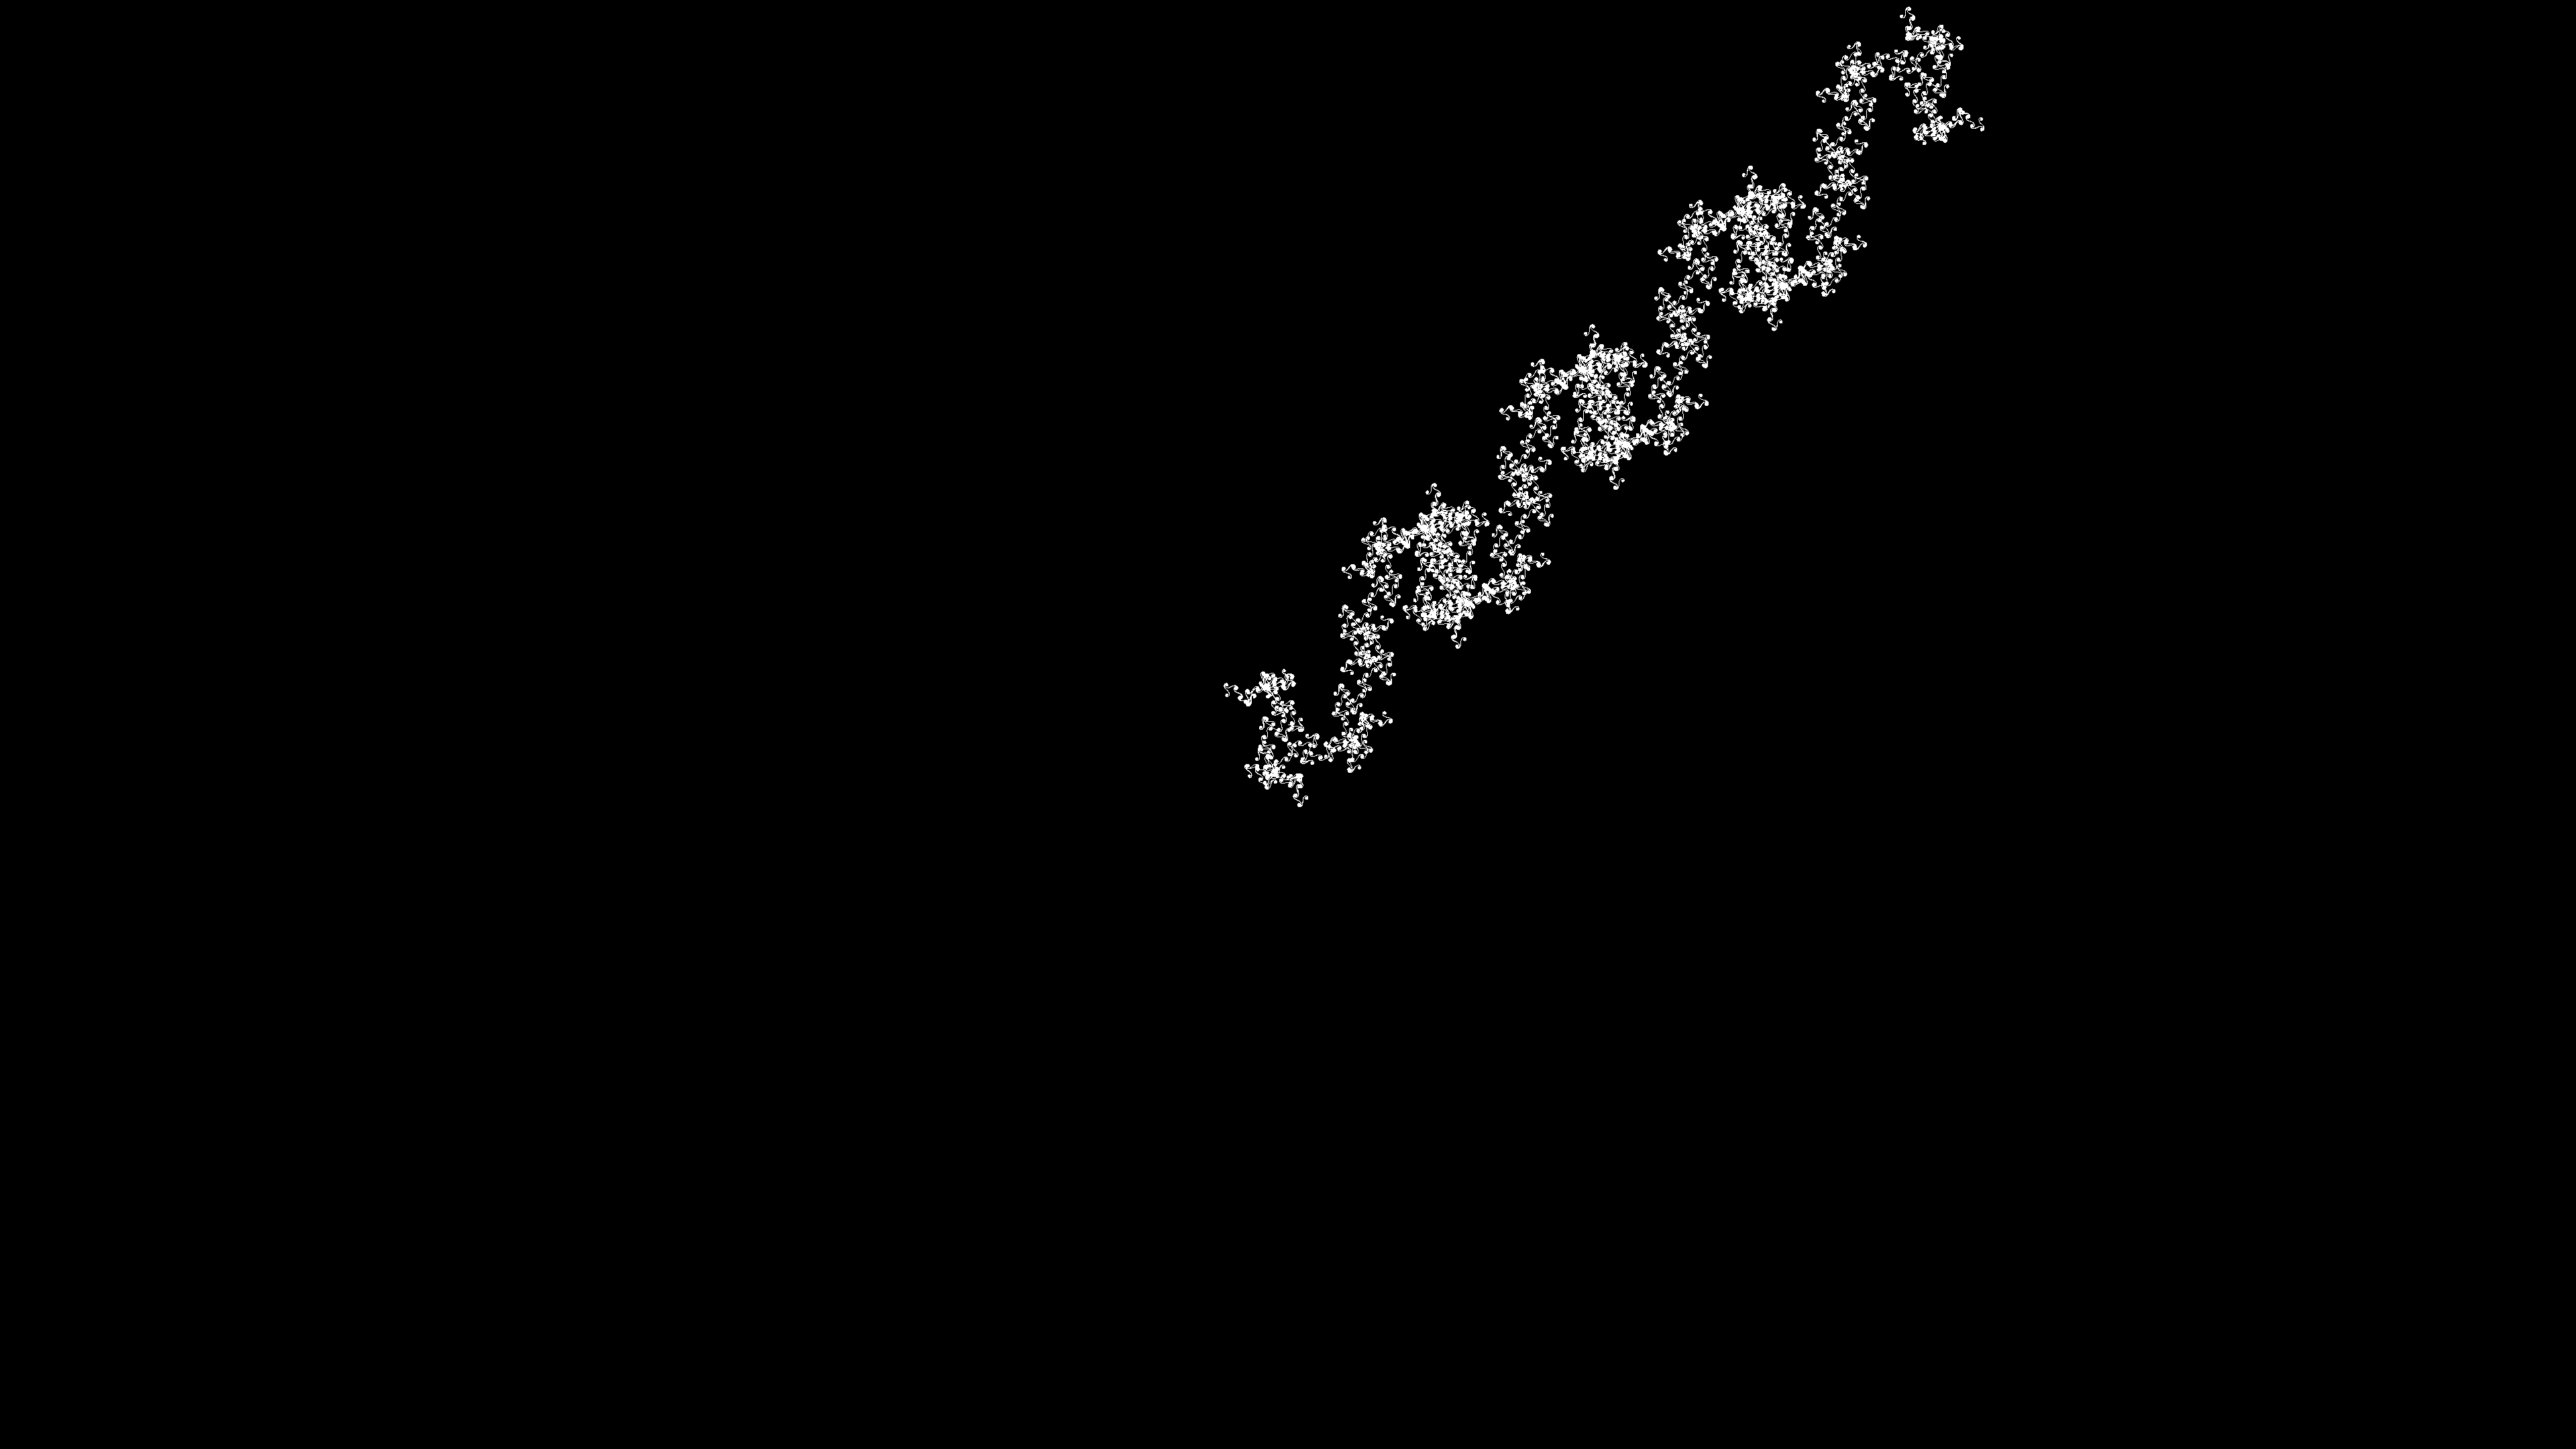
\includegraphics[width=\linewidth]{./stepsplusoneimages/0000000096.png}
    \caption{tf p=499 q=200193 theta=000 89733407.png}
  \end{subfigure}
  \caption{n=094 s=400 s+1=401}
  \label{fig:n=094}
\end{figure}
\begin{figure}[H]
  \centering
  \begin{subfigure}[t]{0.48\textwidth}
    \centering
    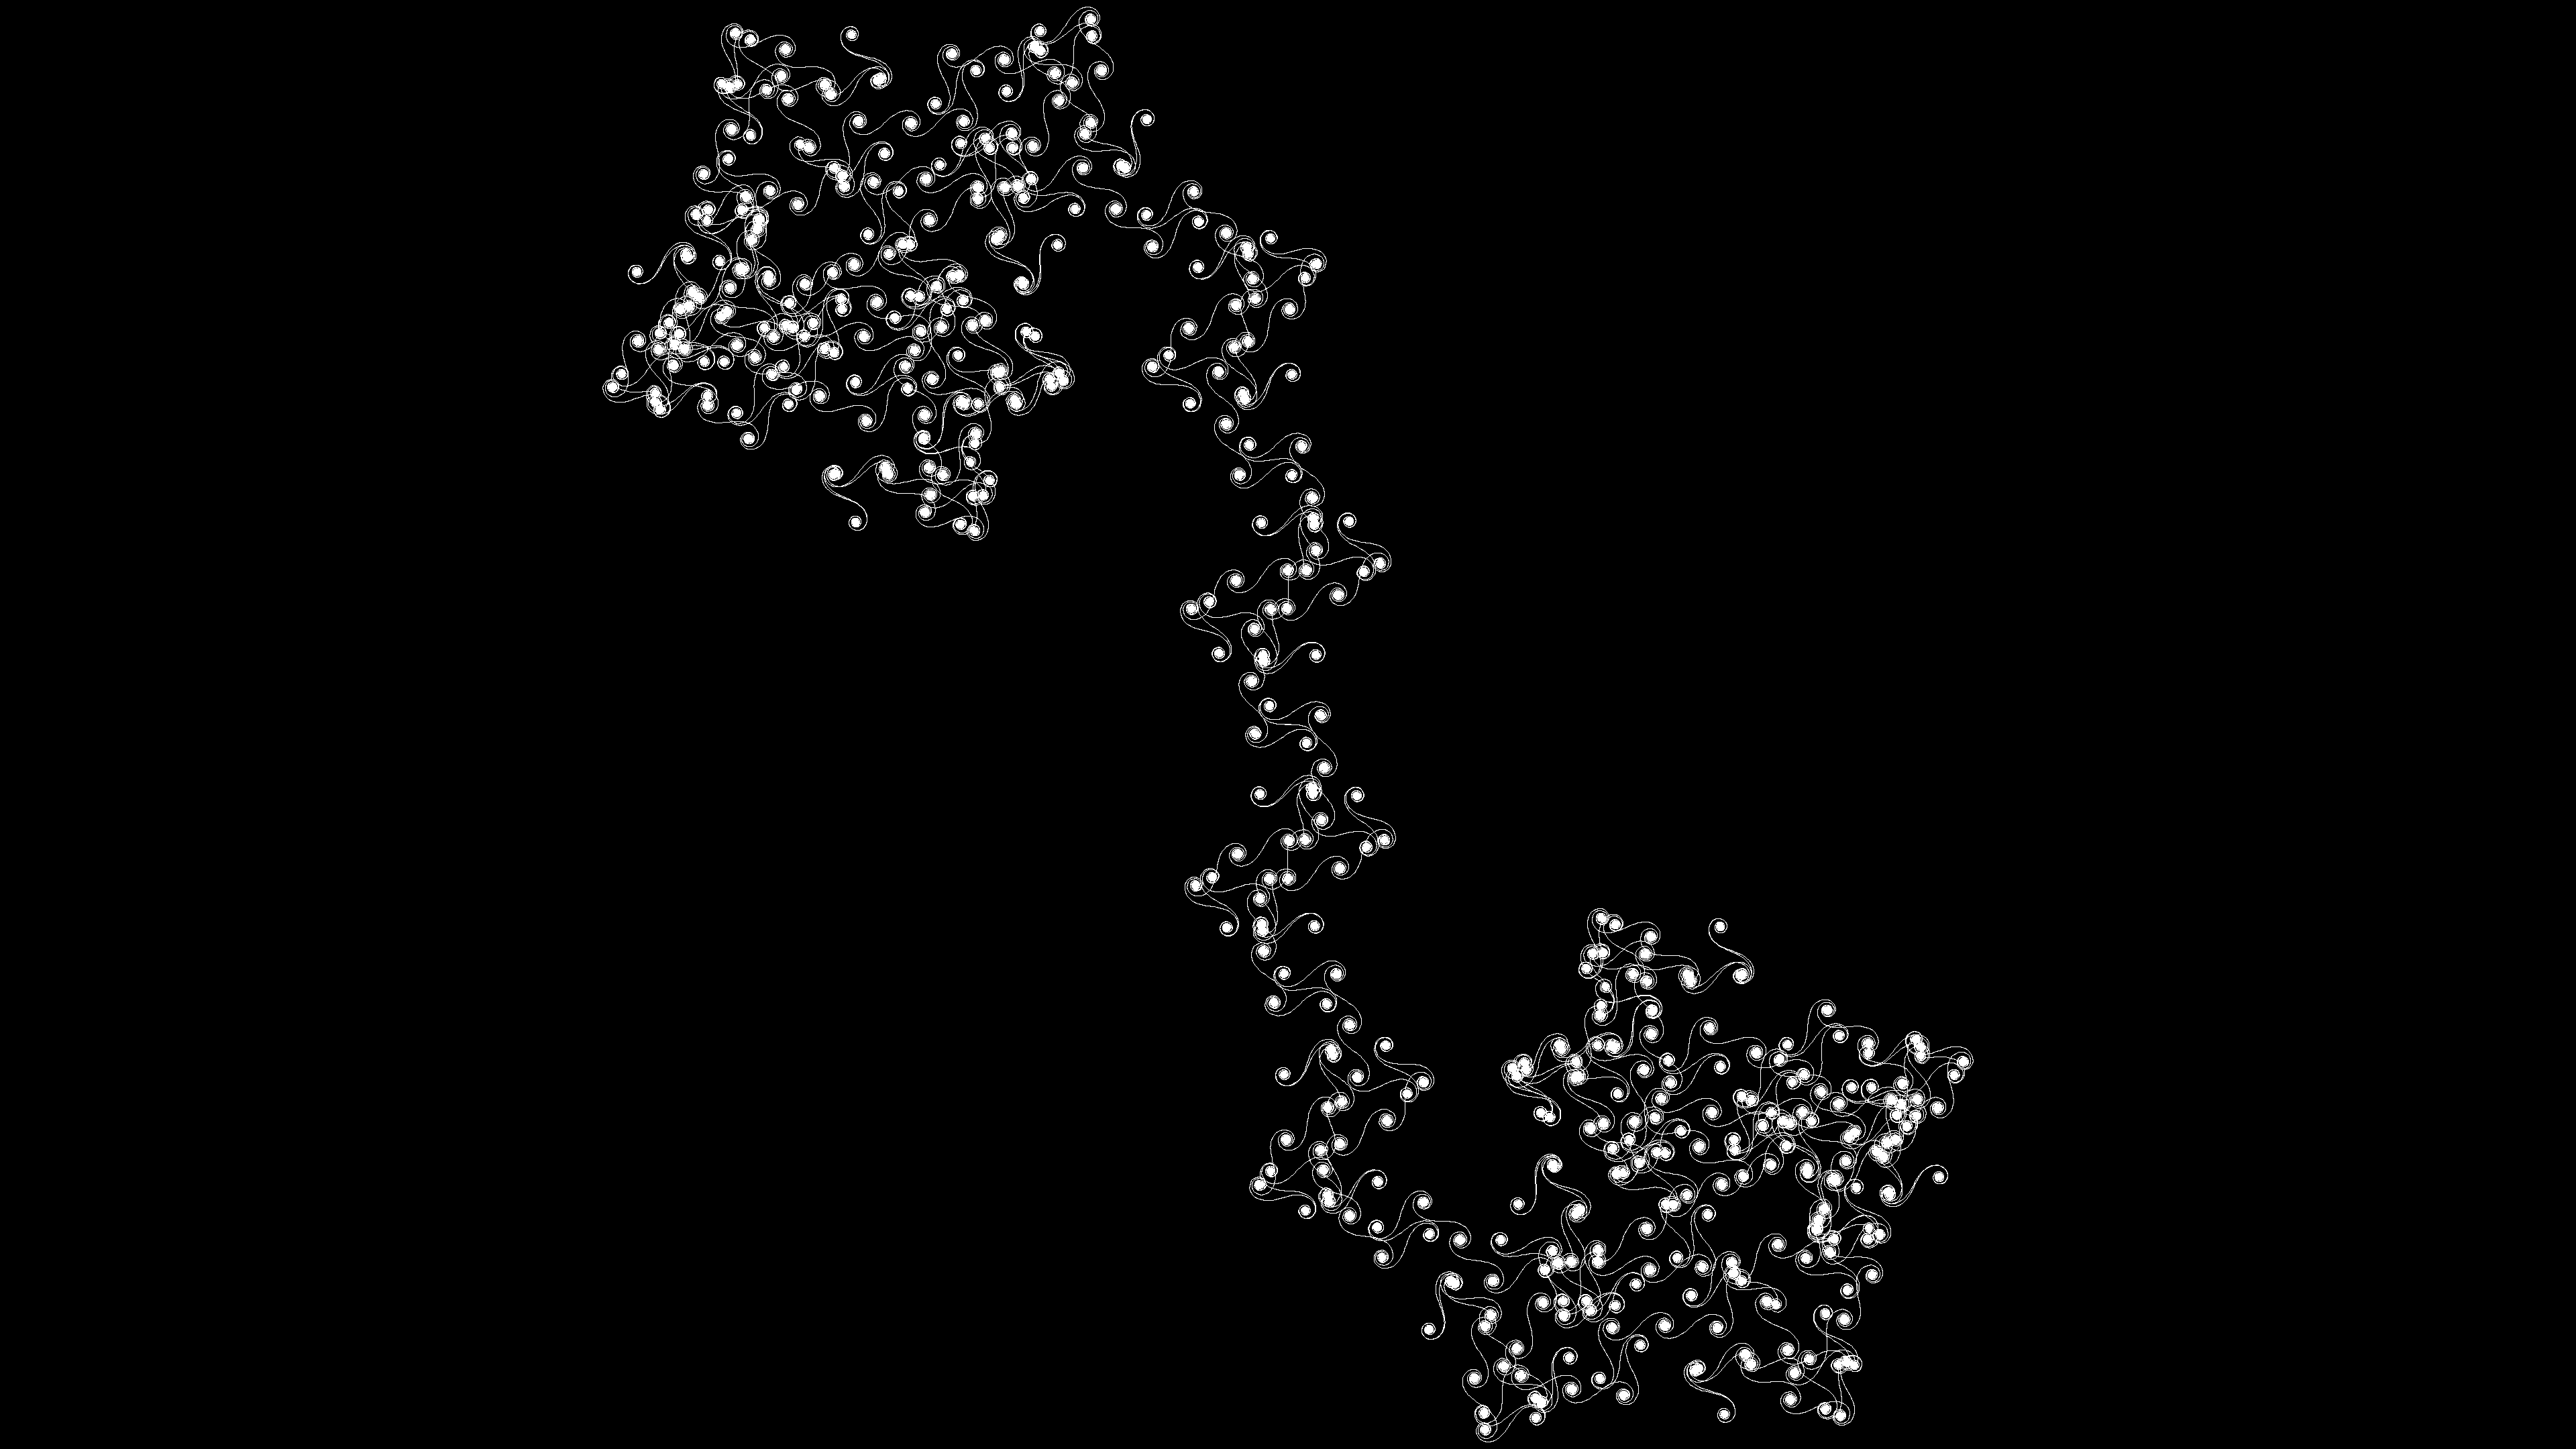
\includegraphics[width=\linewidth]{./stepsplusoneimages/0000000097.png}
    \caption{tf p=499 q=199696 theta=000 89956734.png}
  \end{subfigure}
  \begin{subfigure}[t]{0.48\textwidth}
    \centering
    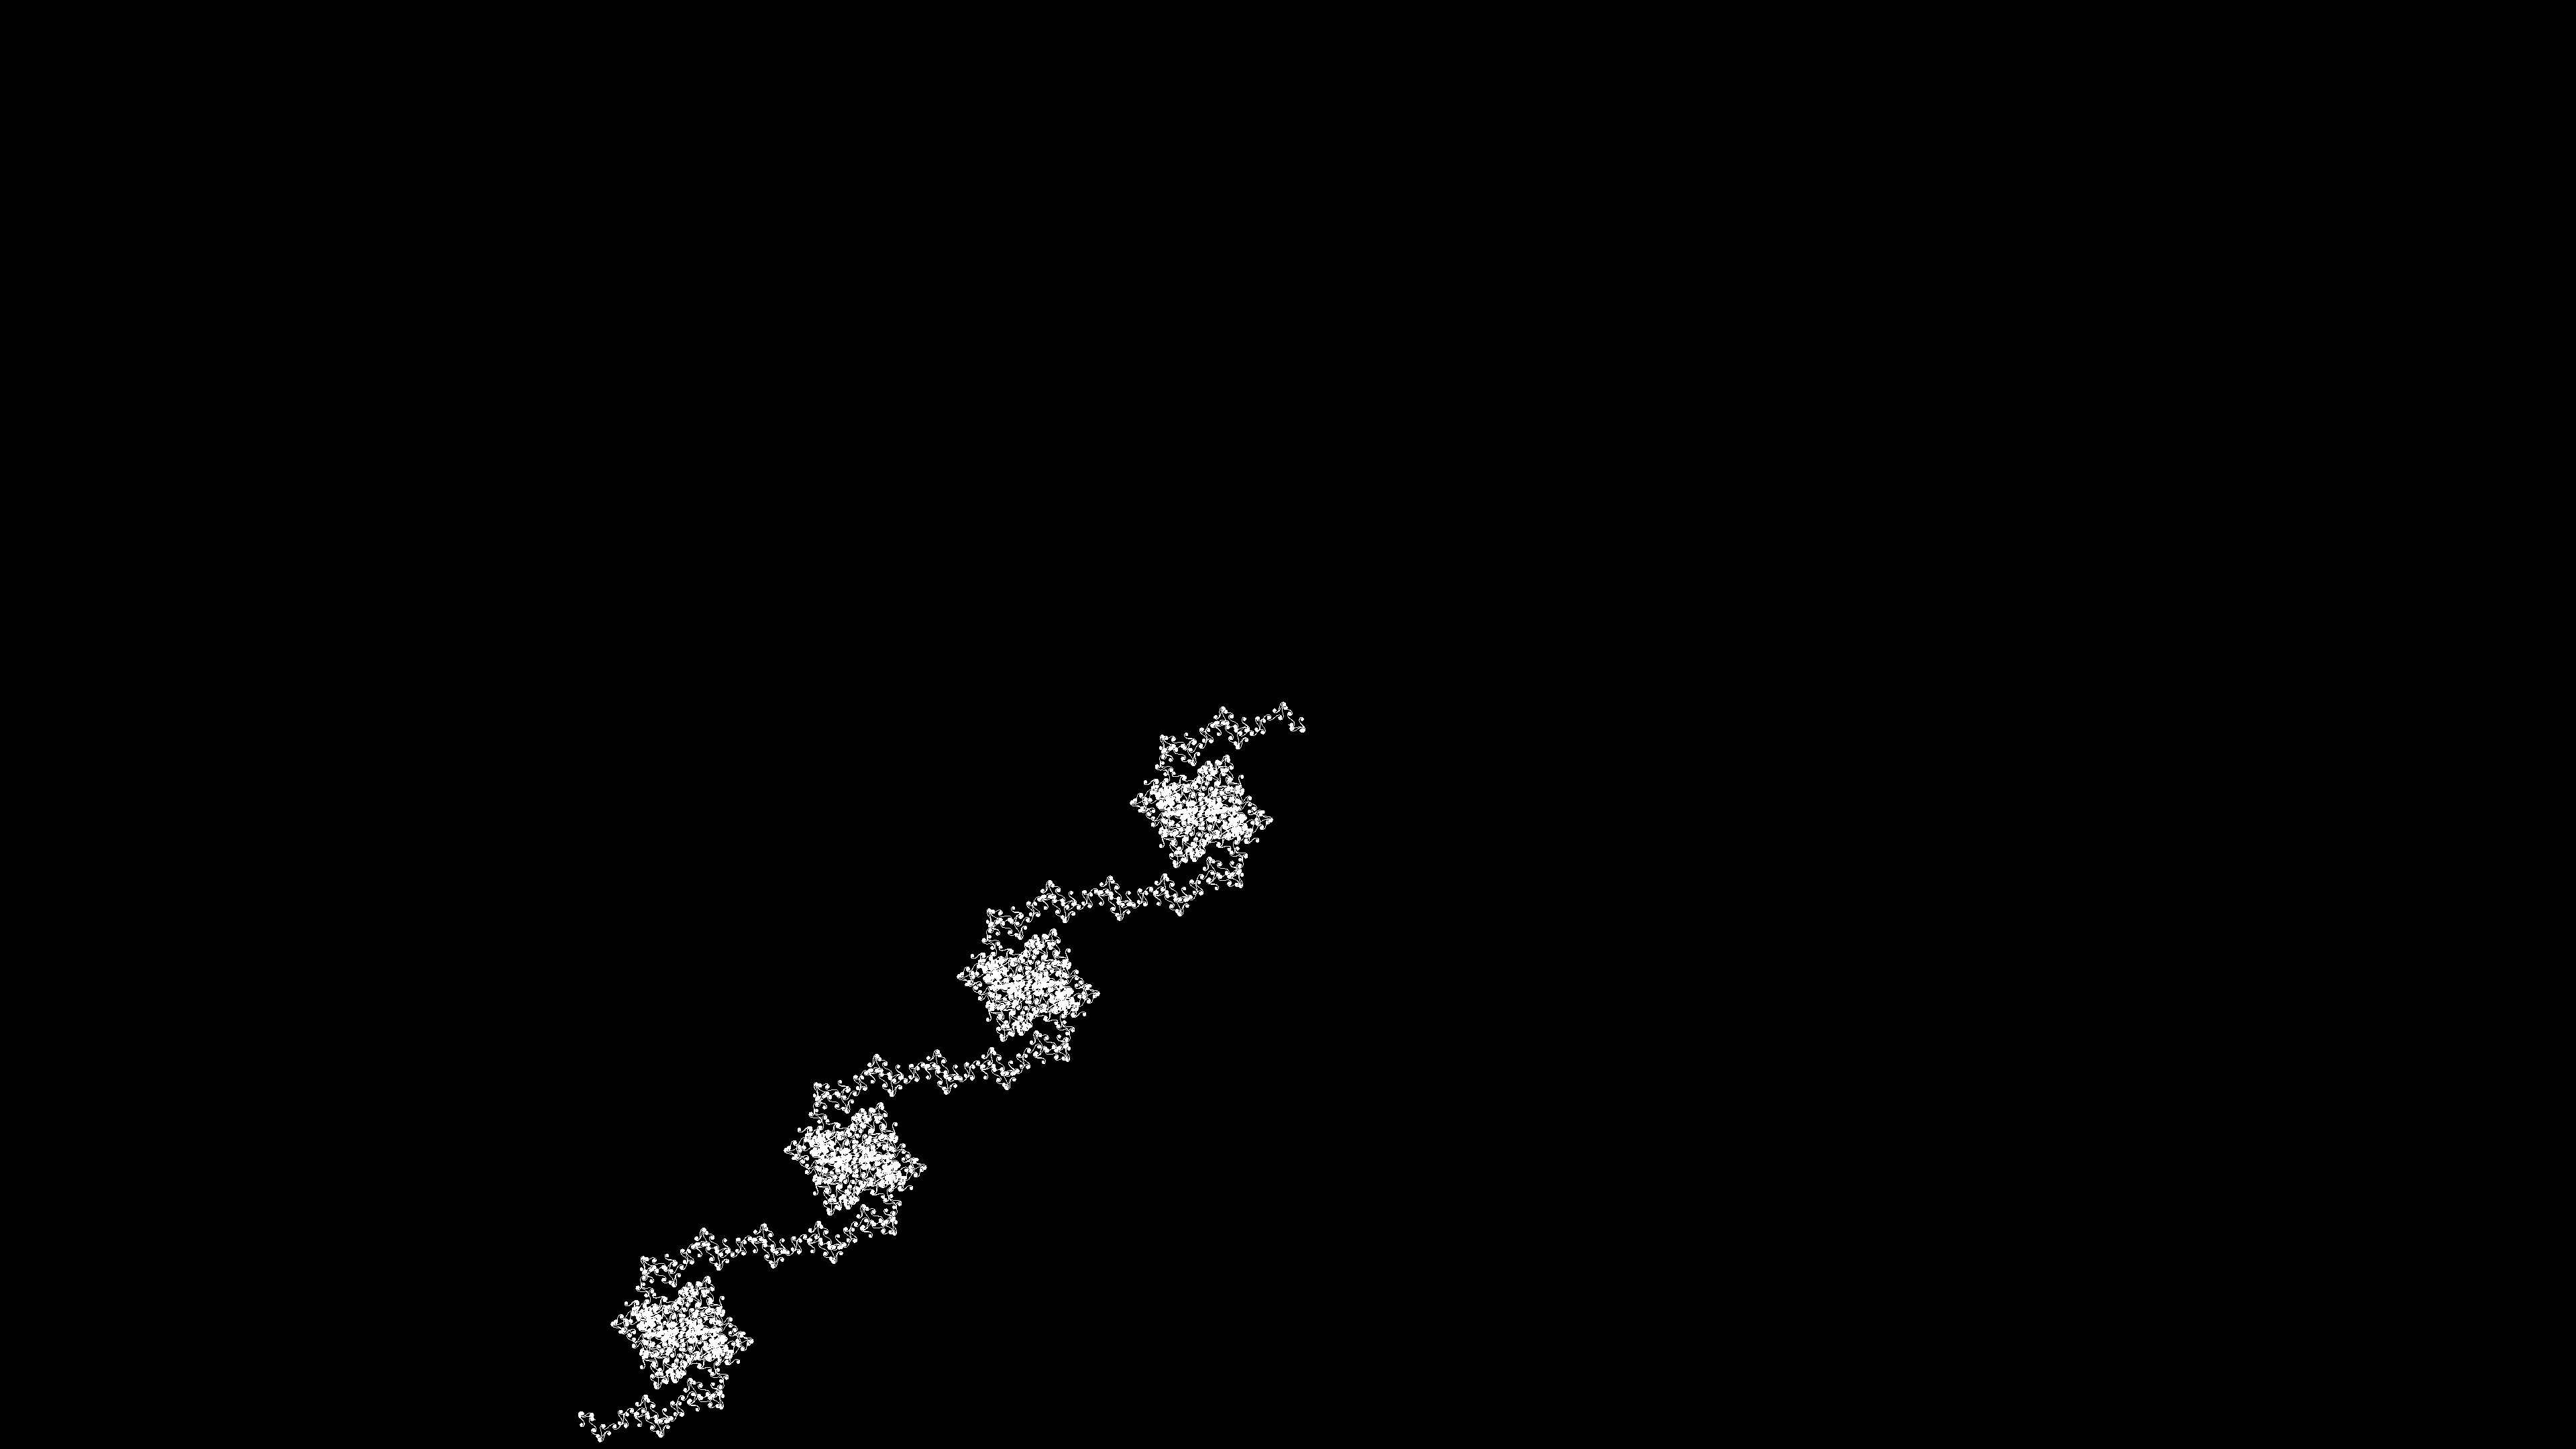
\includegraphics[width=\linewidth]{./stepsplusoneimages/0000000098.png}
    \caption{tf p=499 q=200195 theta=000 89732511.png}
  \end{subfigure}
  \caption{n=096 s=400 s+1=401}
  \label{fig:n=096}
\end{figure}
\begin{figure}[H]
  \centering
  \begin{subfigure}[t]{0.48\textwidth}
    \centering
    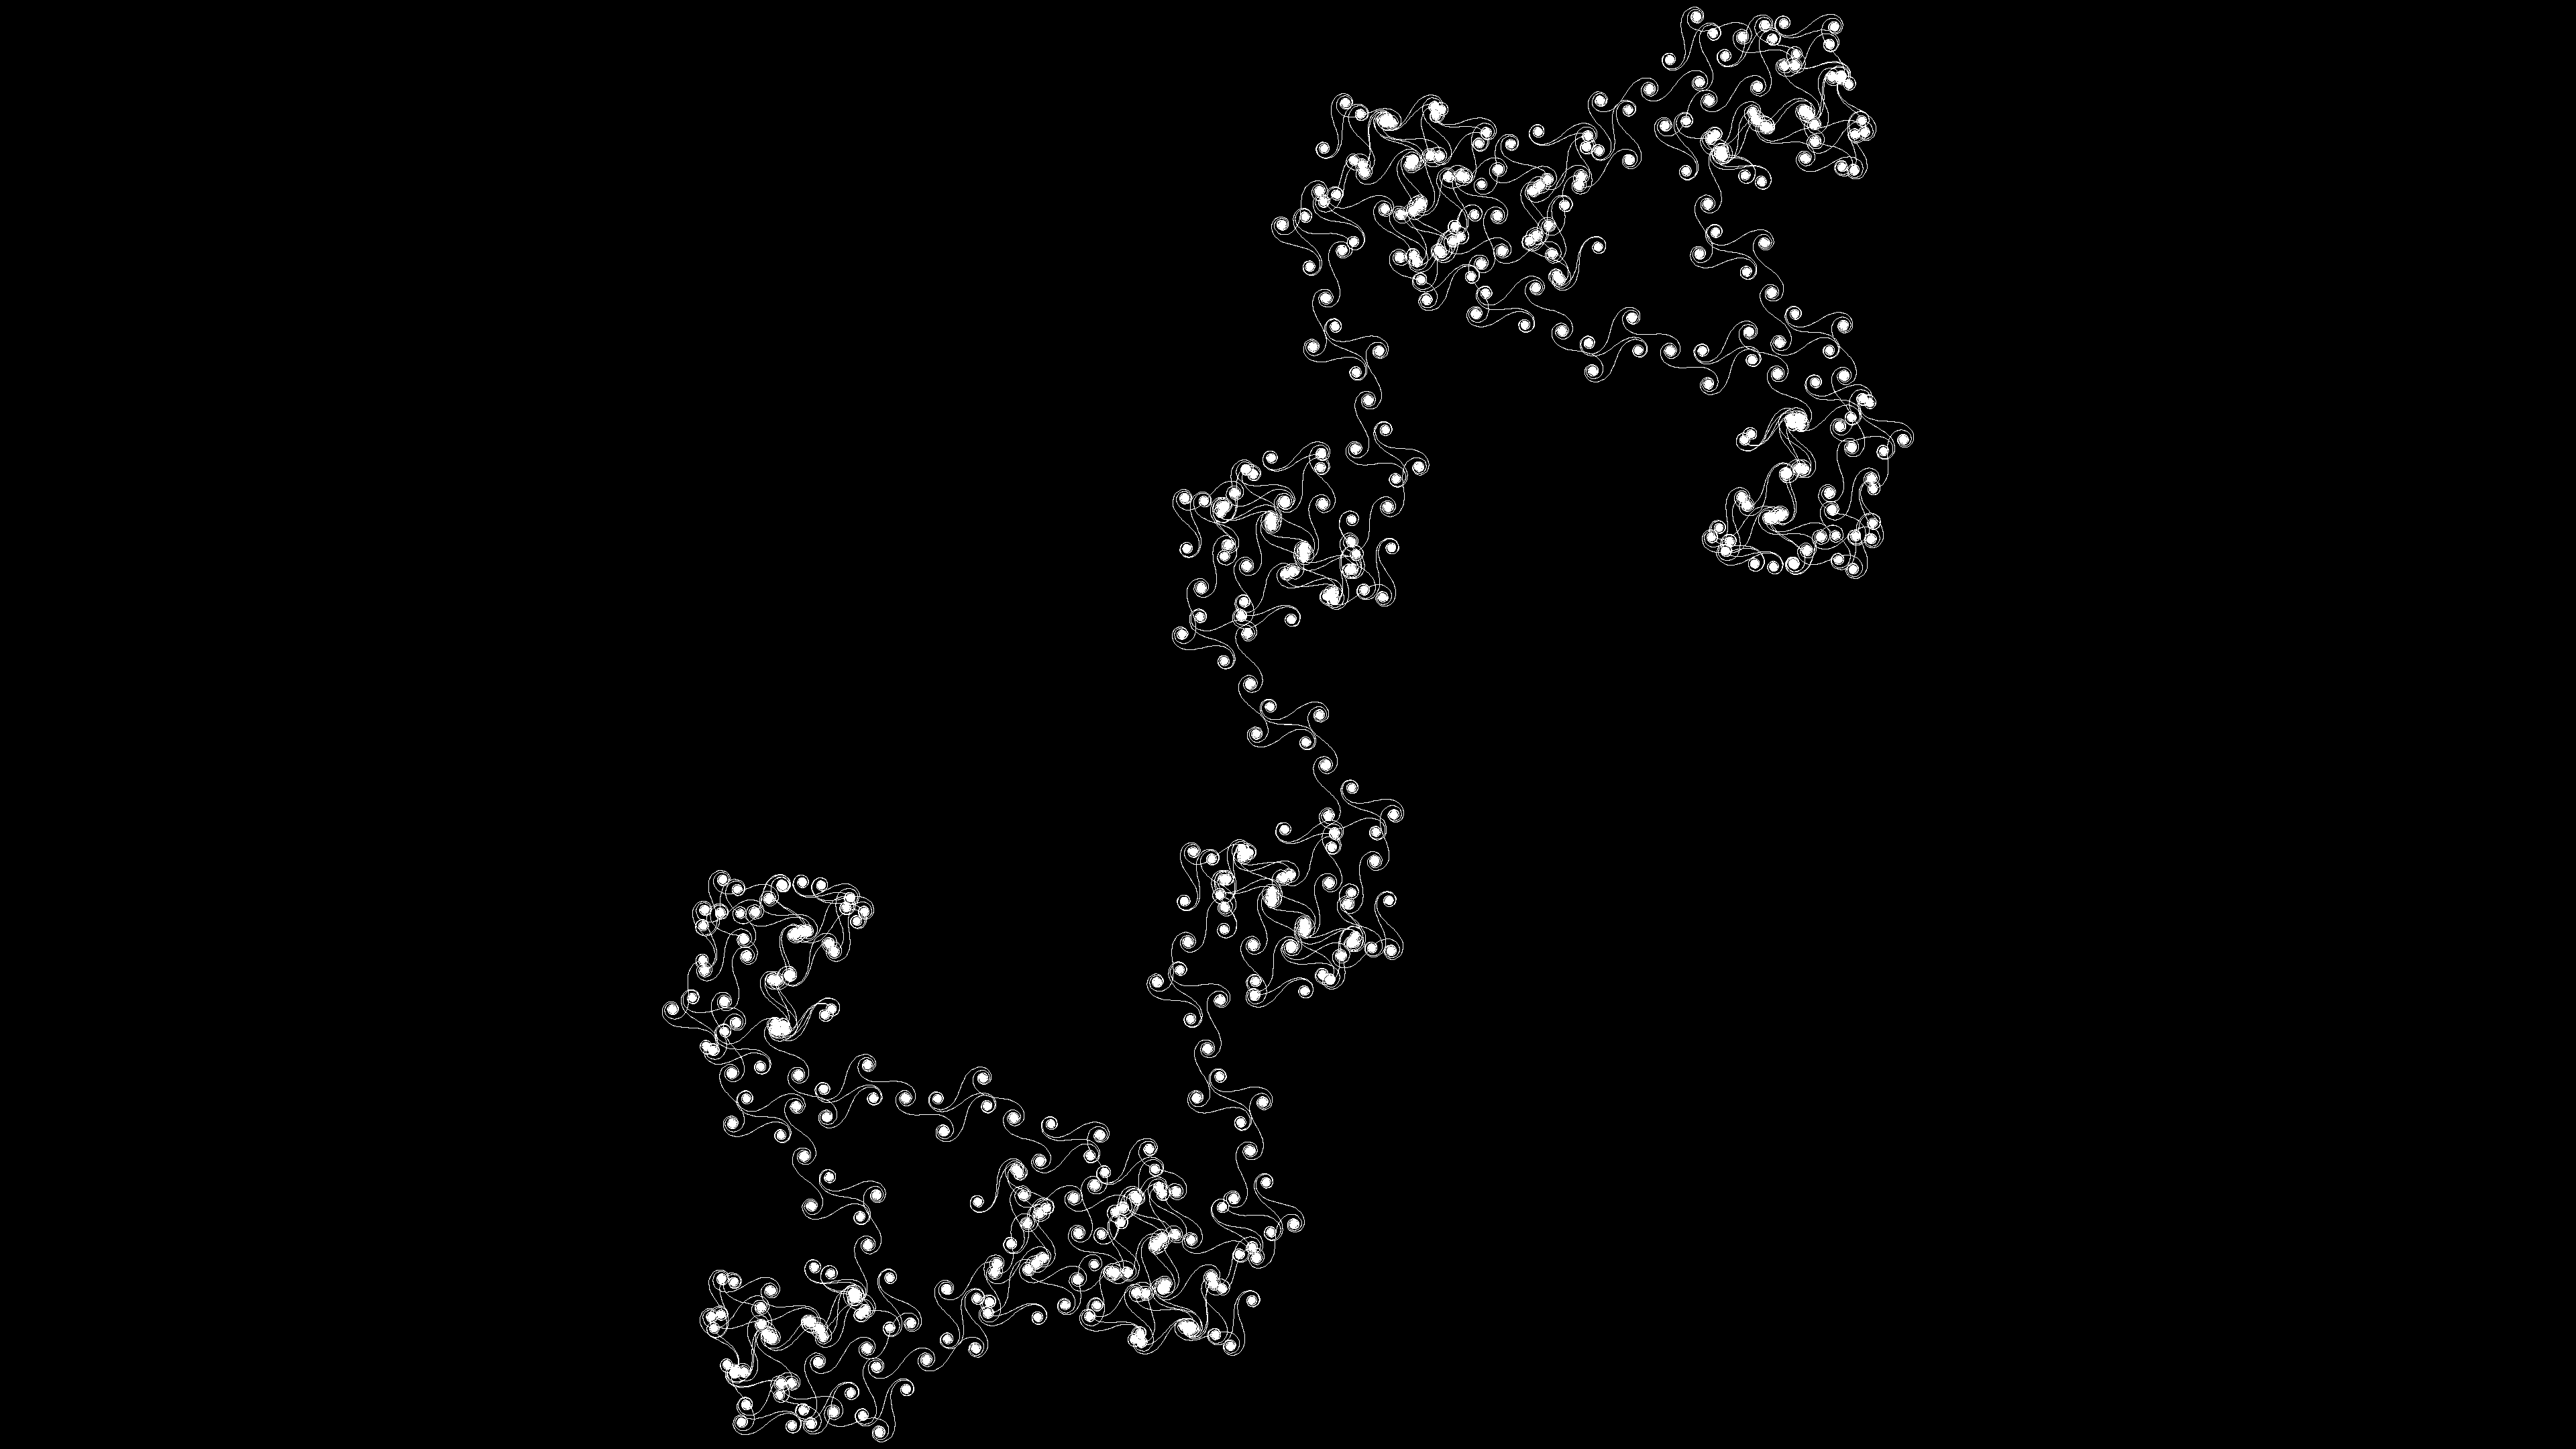
\includegraphics[width=\linewidth]{./stepsplusoneimages/0000000099.png}
    \caption{tf p=499 q=199698 theta=000 89955833.png}
  \end{subfigure}
  \begin{subfigure}[t]{0.48\textwidth}
    \centering
    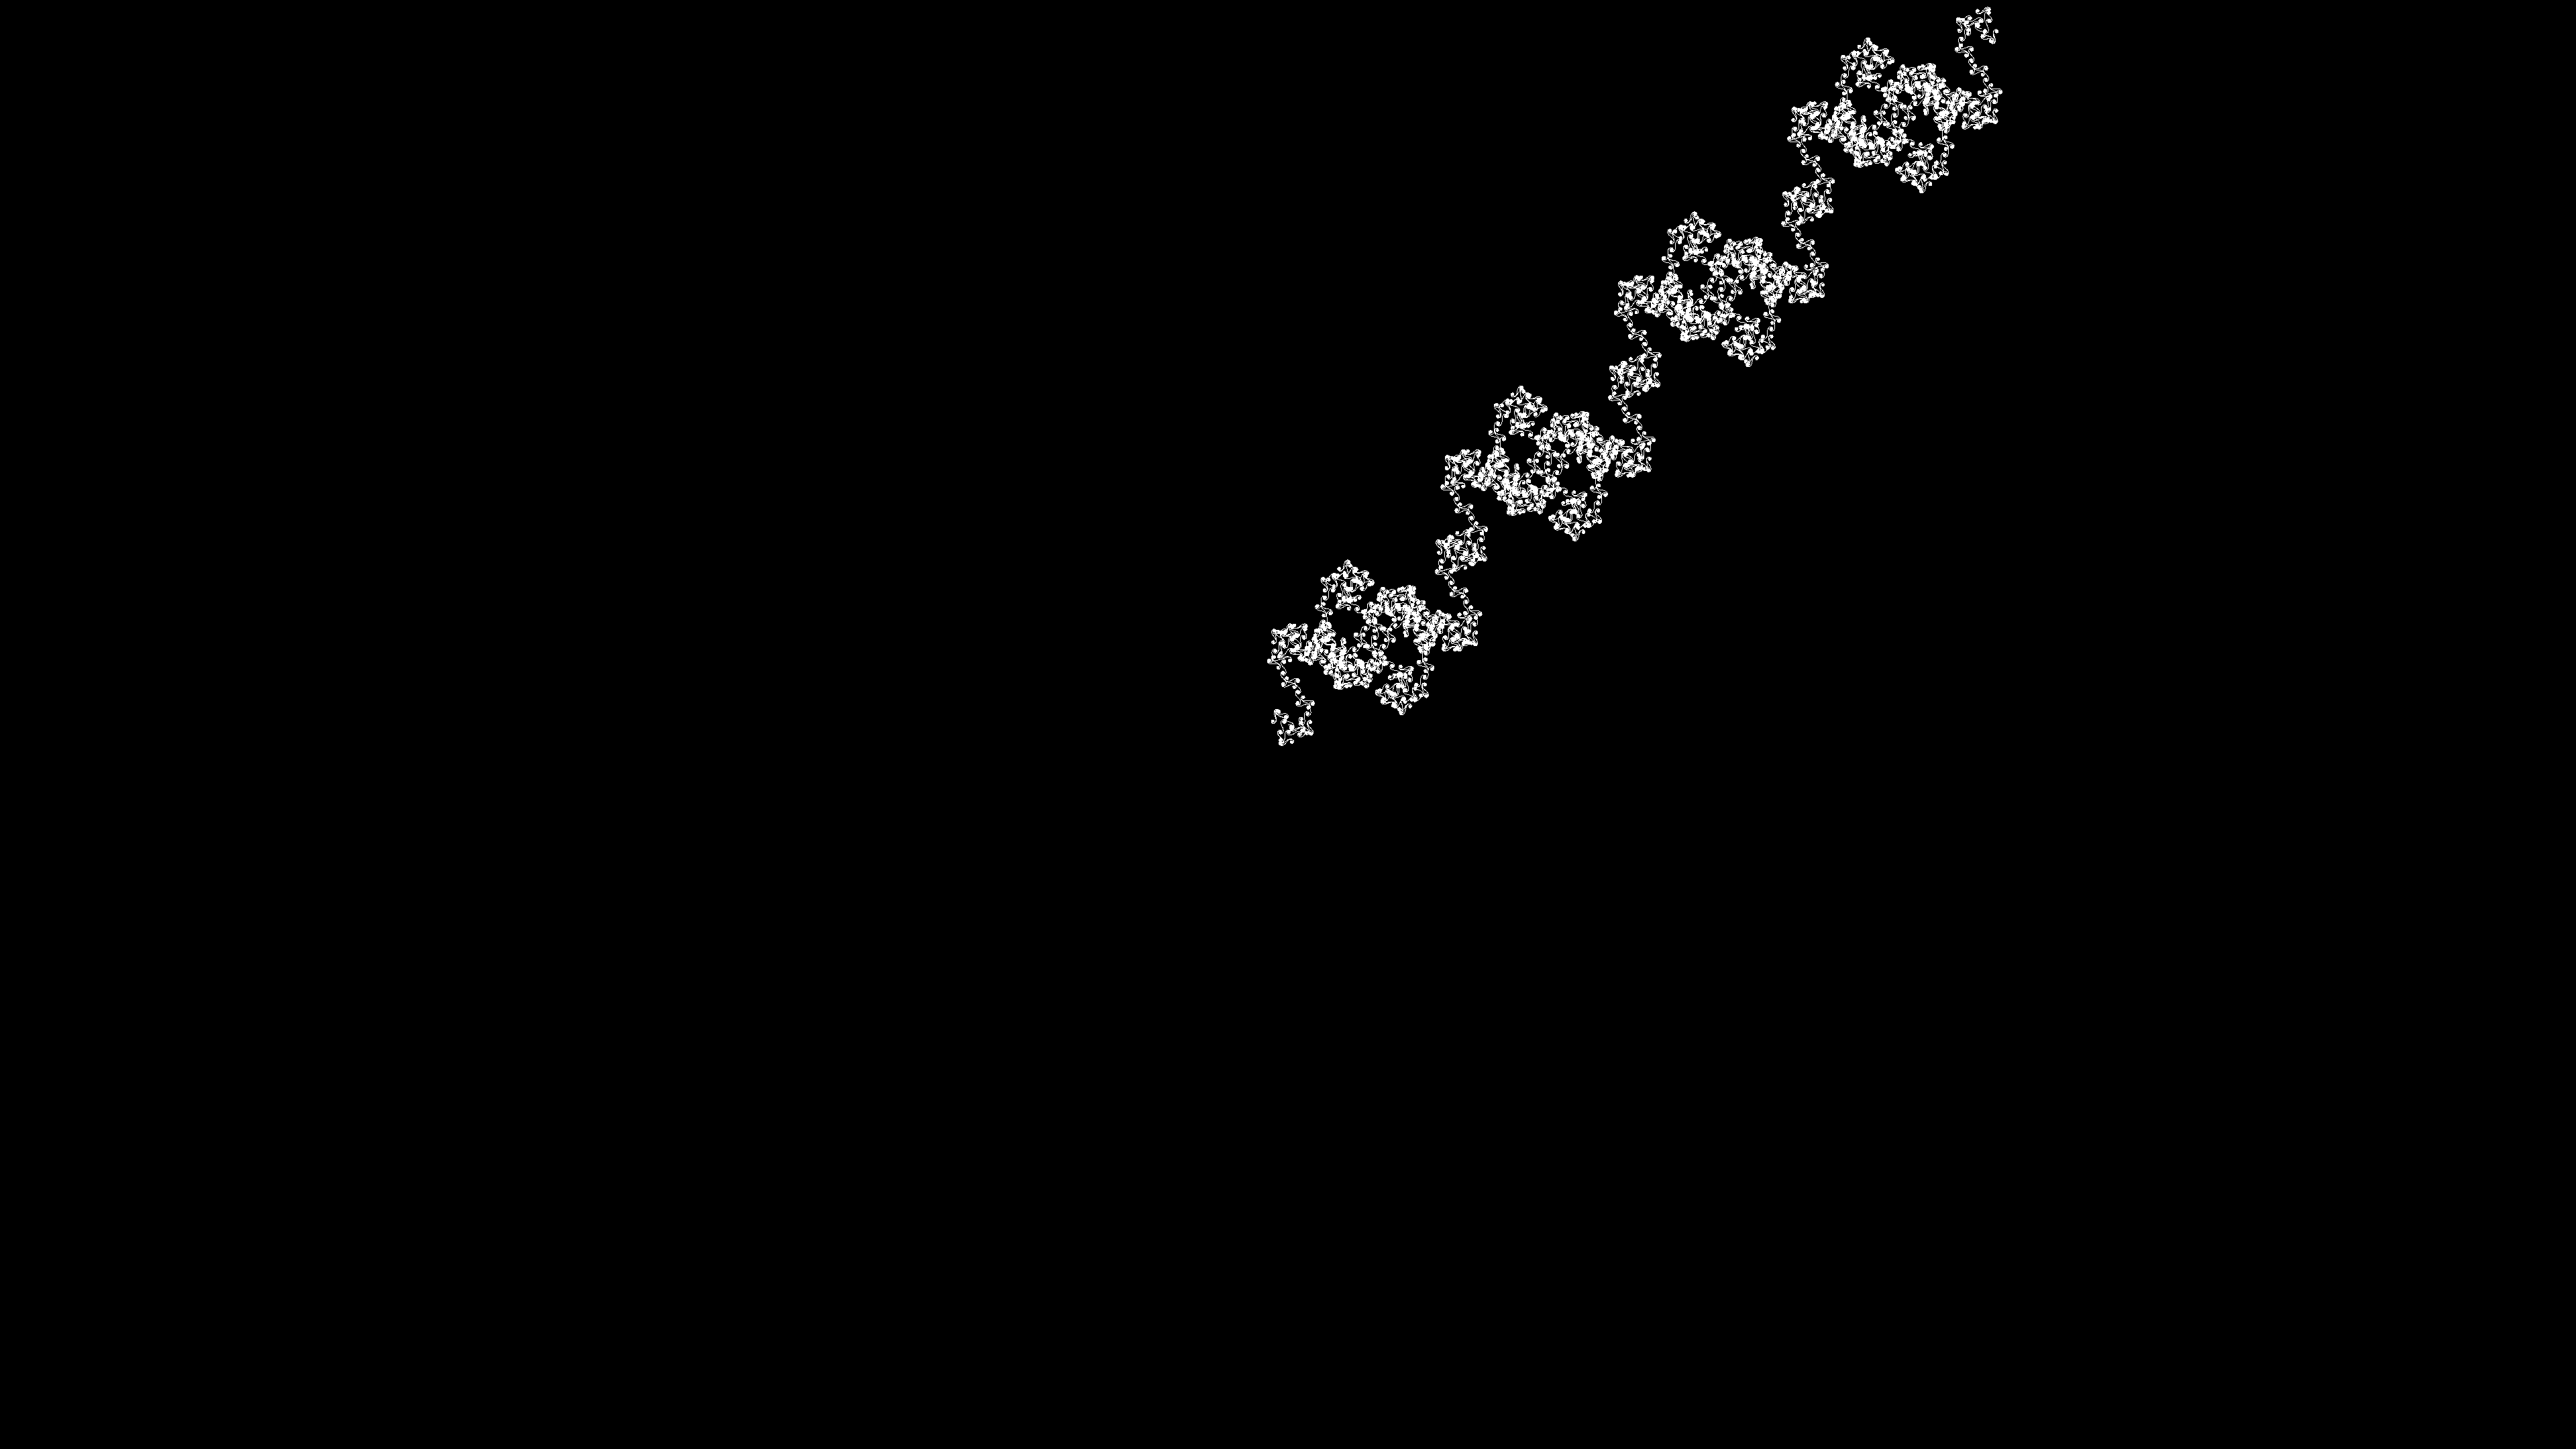
\includegraphics[width=\linewidth]{./stepsplusoneimages/0000000100.png}
    \caption{tf p=499 q=200197 theta=000 89731614.png}
  \end{subfigure}
  \caption{n=098 s=400 s+1=401}
  \label{fig:n=098}
\end{figure}
\begin{figure}[H]
  \centering
  \begin{subfigure}[t]{0.48\textwidth}
    \centering
    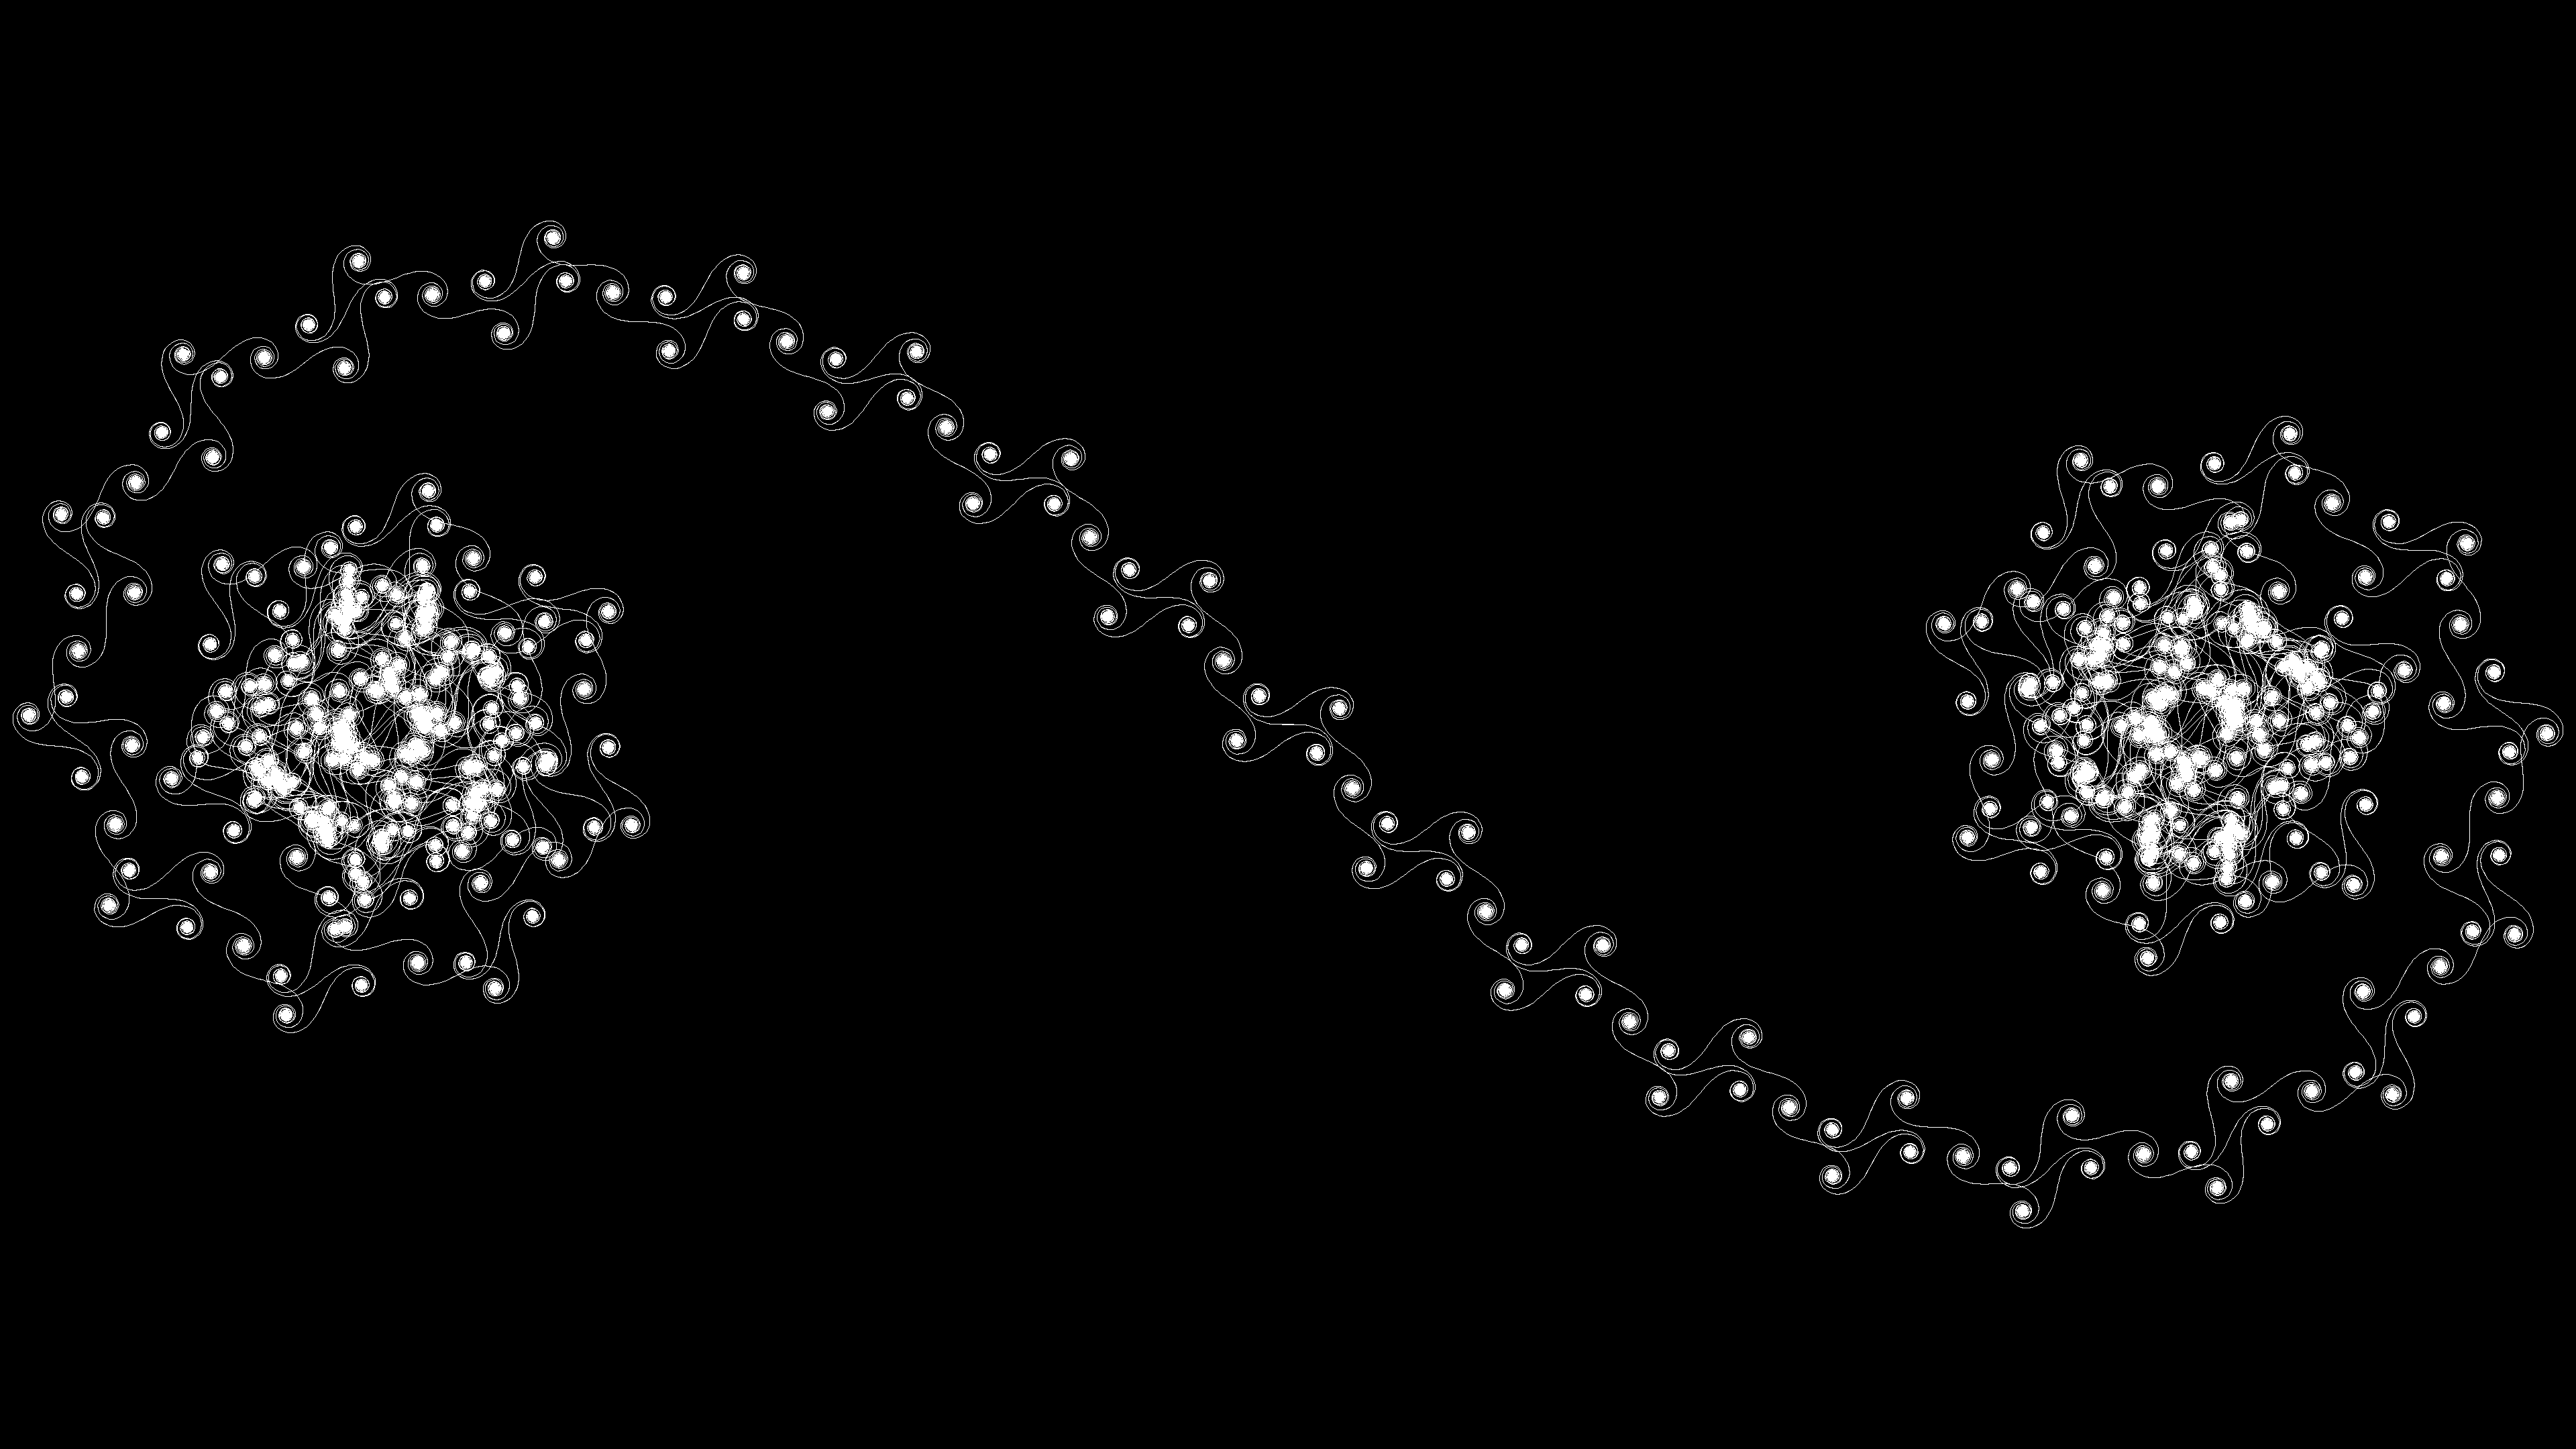
\includegraphics[width=\linewidth]{./stepsplusoneimages/0000000101.png}
    \caption{tf p=499 q=199700 theta=000 89954932.png}
  \end{subfigure}
  \begin{subfigure}[t]{0.48\textwidth}
    \centering
    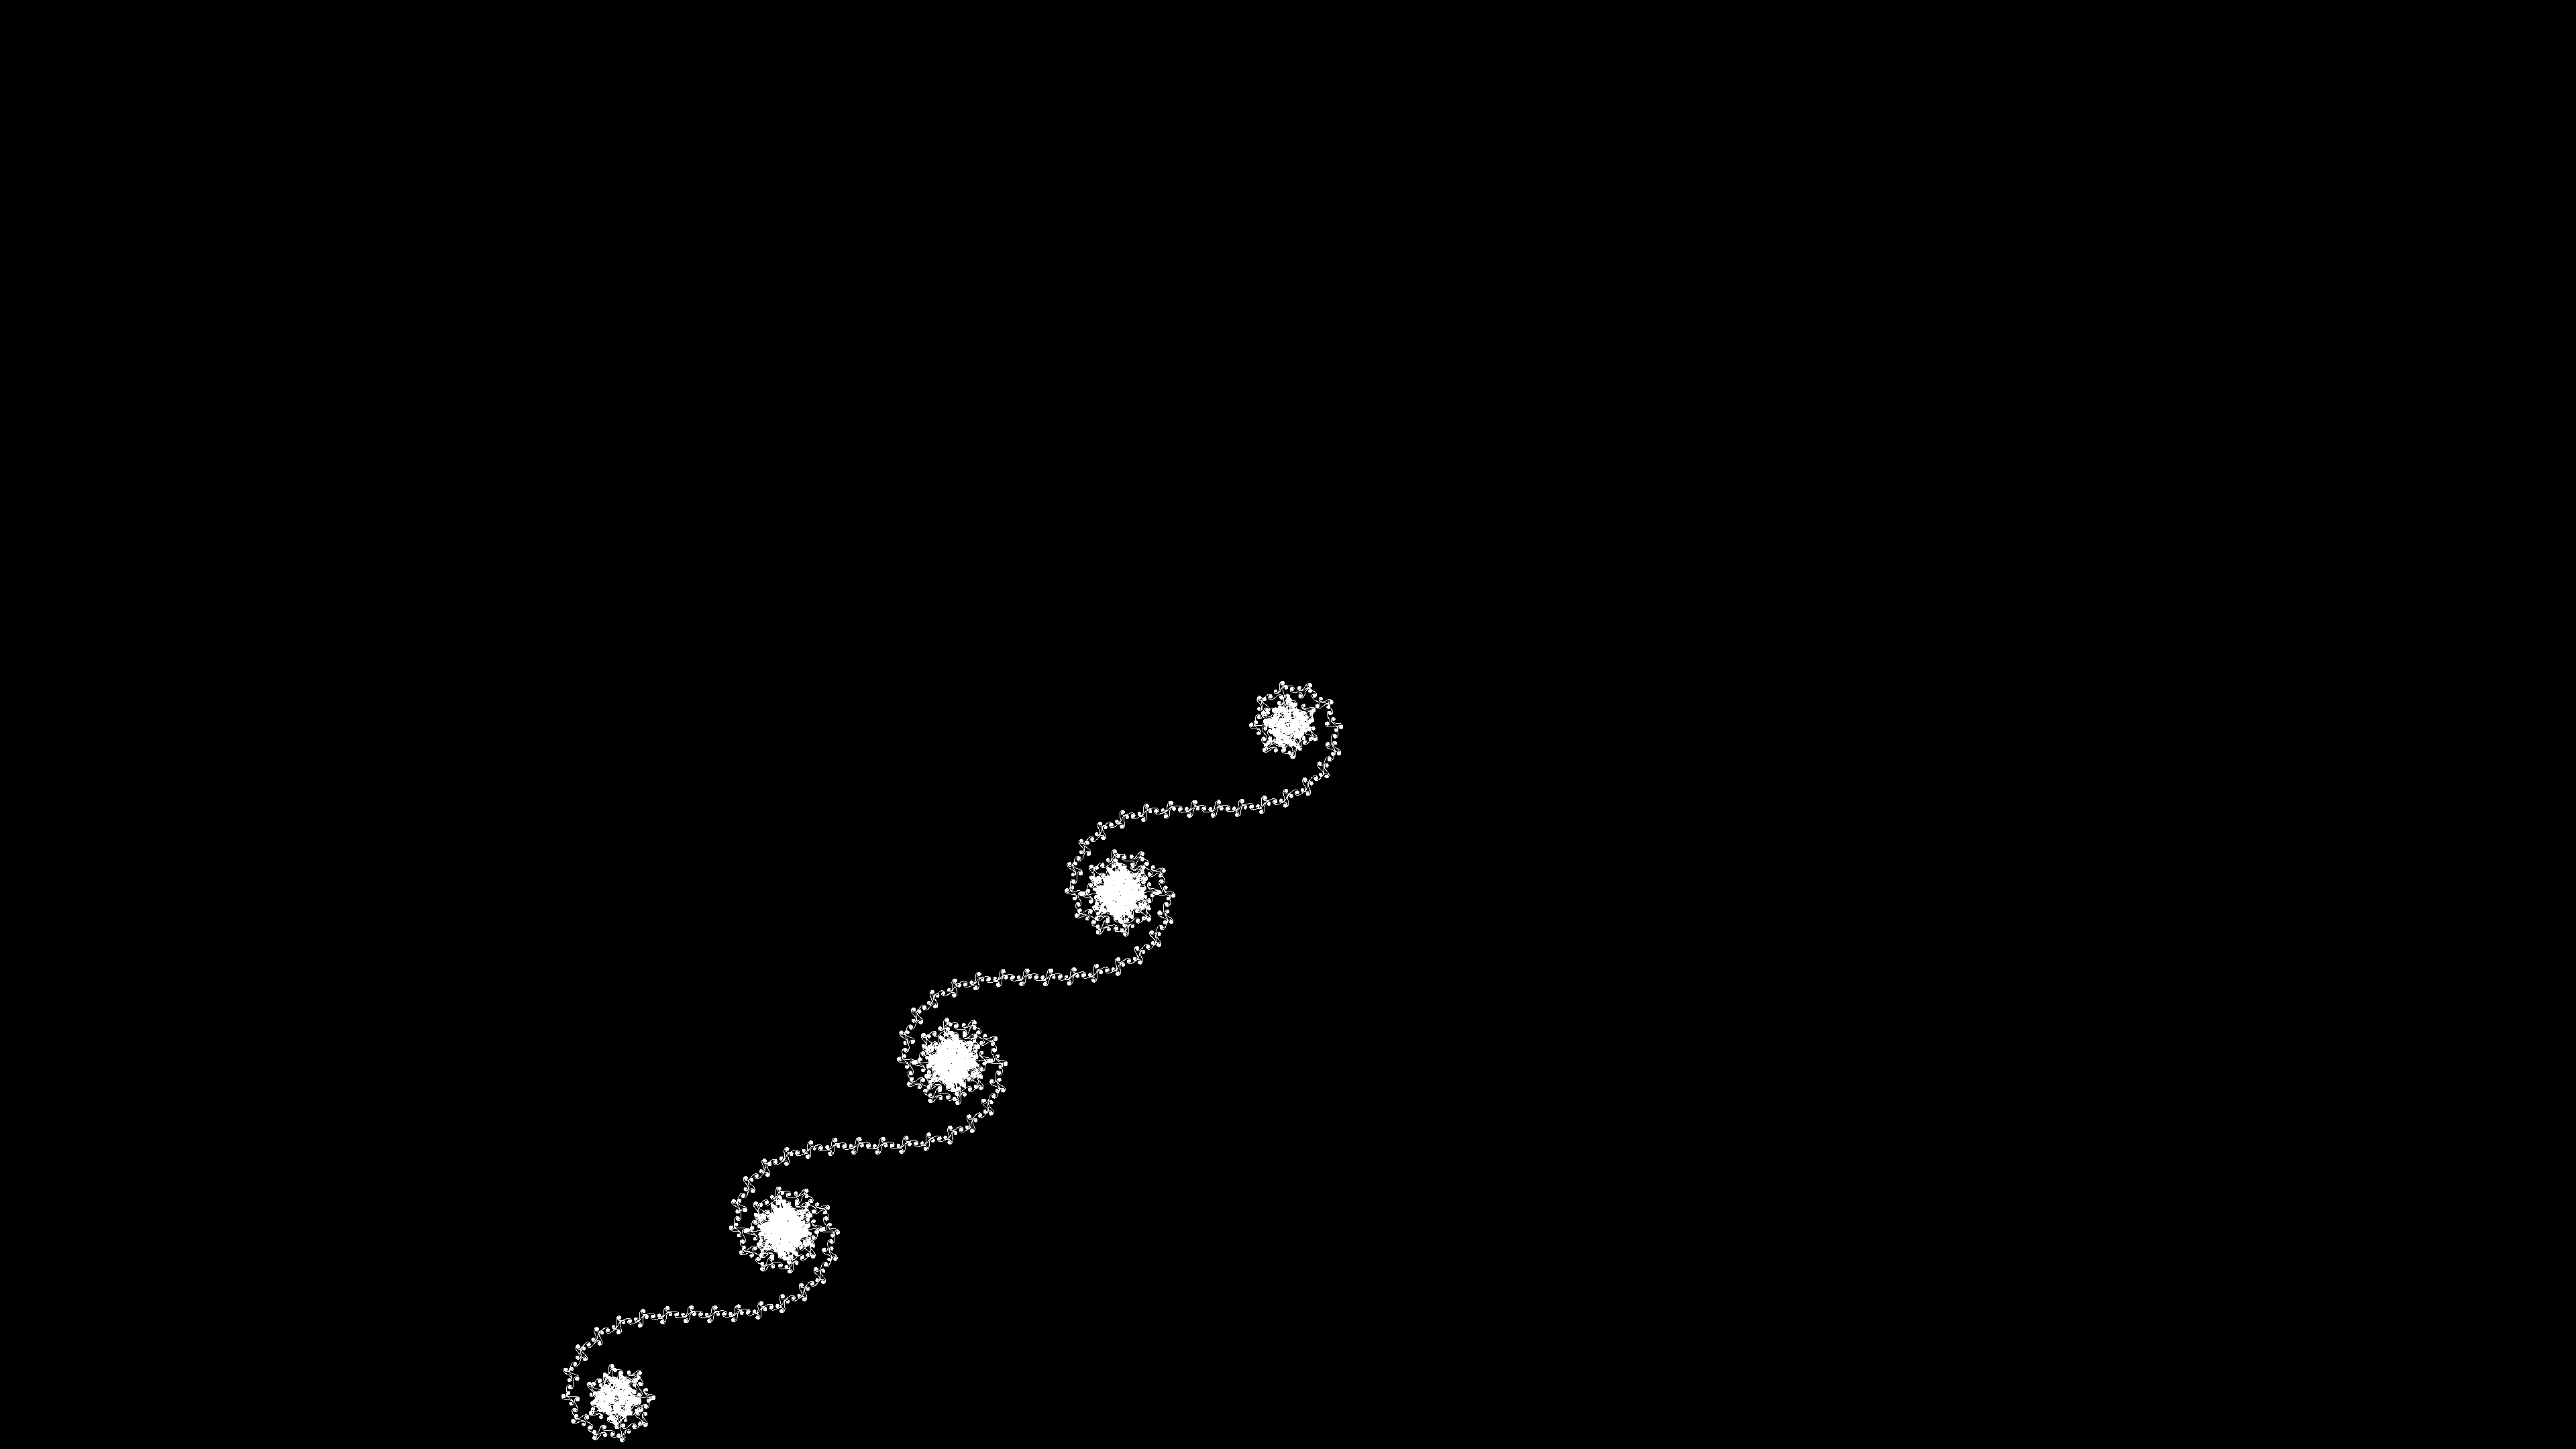
\includegraphics[width=\linewidth]{./stepsplusoneimages/0000000102.png}
    \caption{tf p=499 q=200199 theta=000 89730718.png}
  \end{subfigure}
  \caption{n=100 s=400 s+1=401}
  \label{fig:n=100}
\end{figure}
\begin{figure}[H]
  \centering
  \begin{subfigure}[t]{0.48\textwidth}
    \centering
    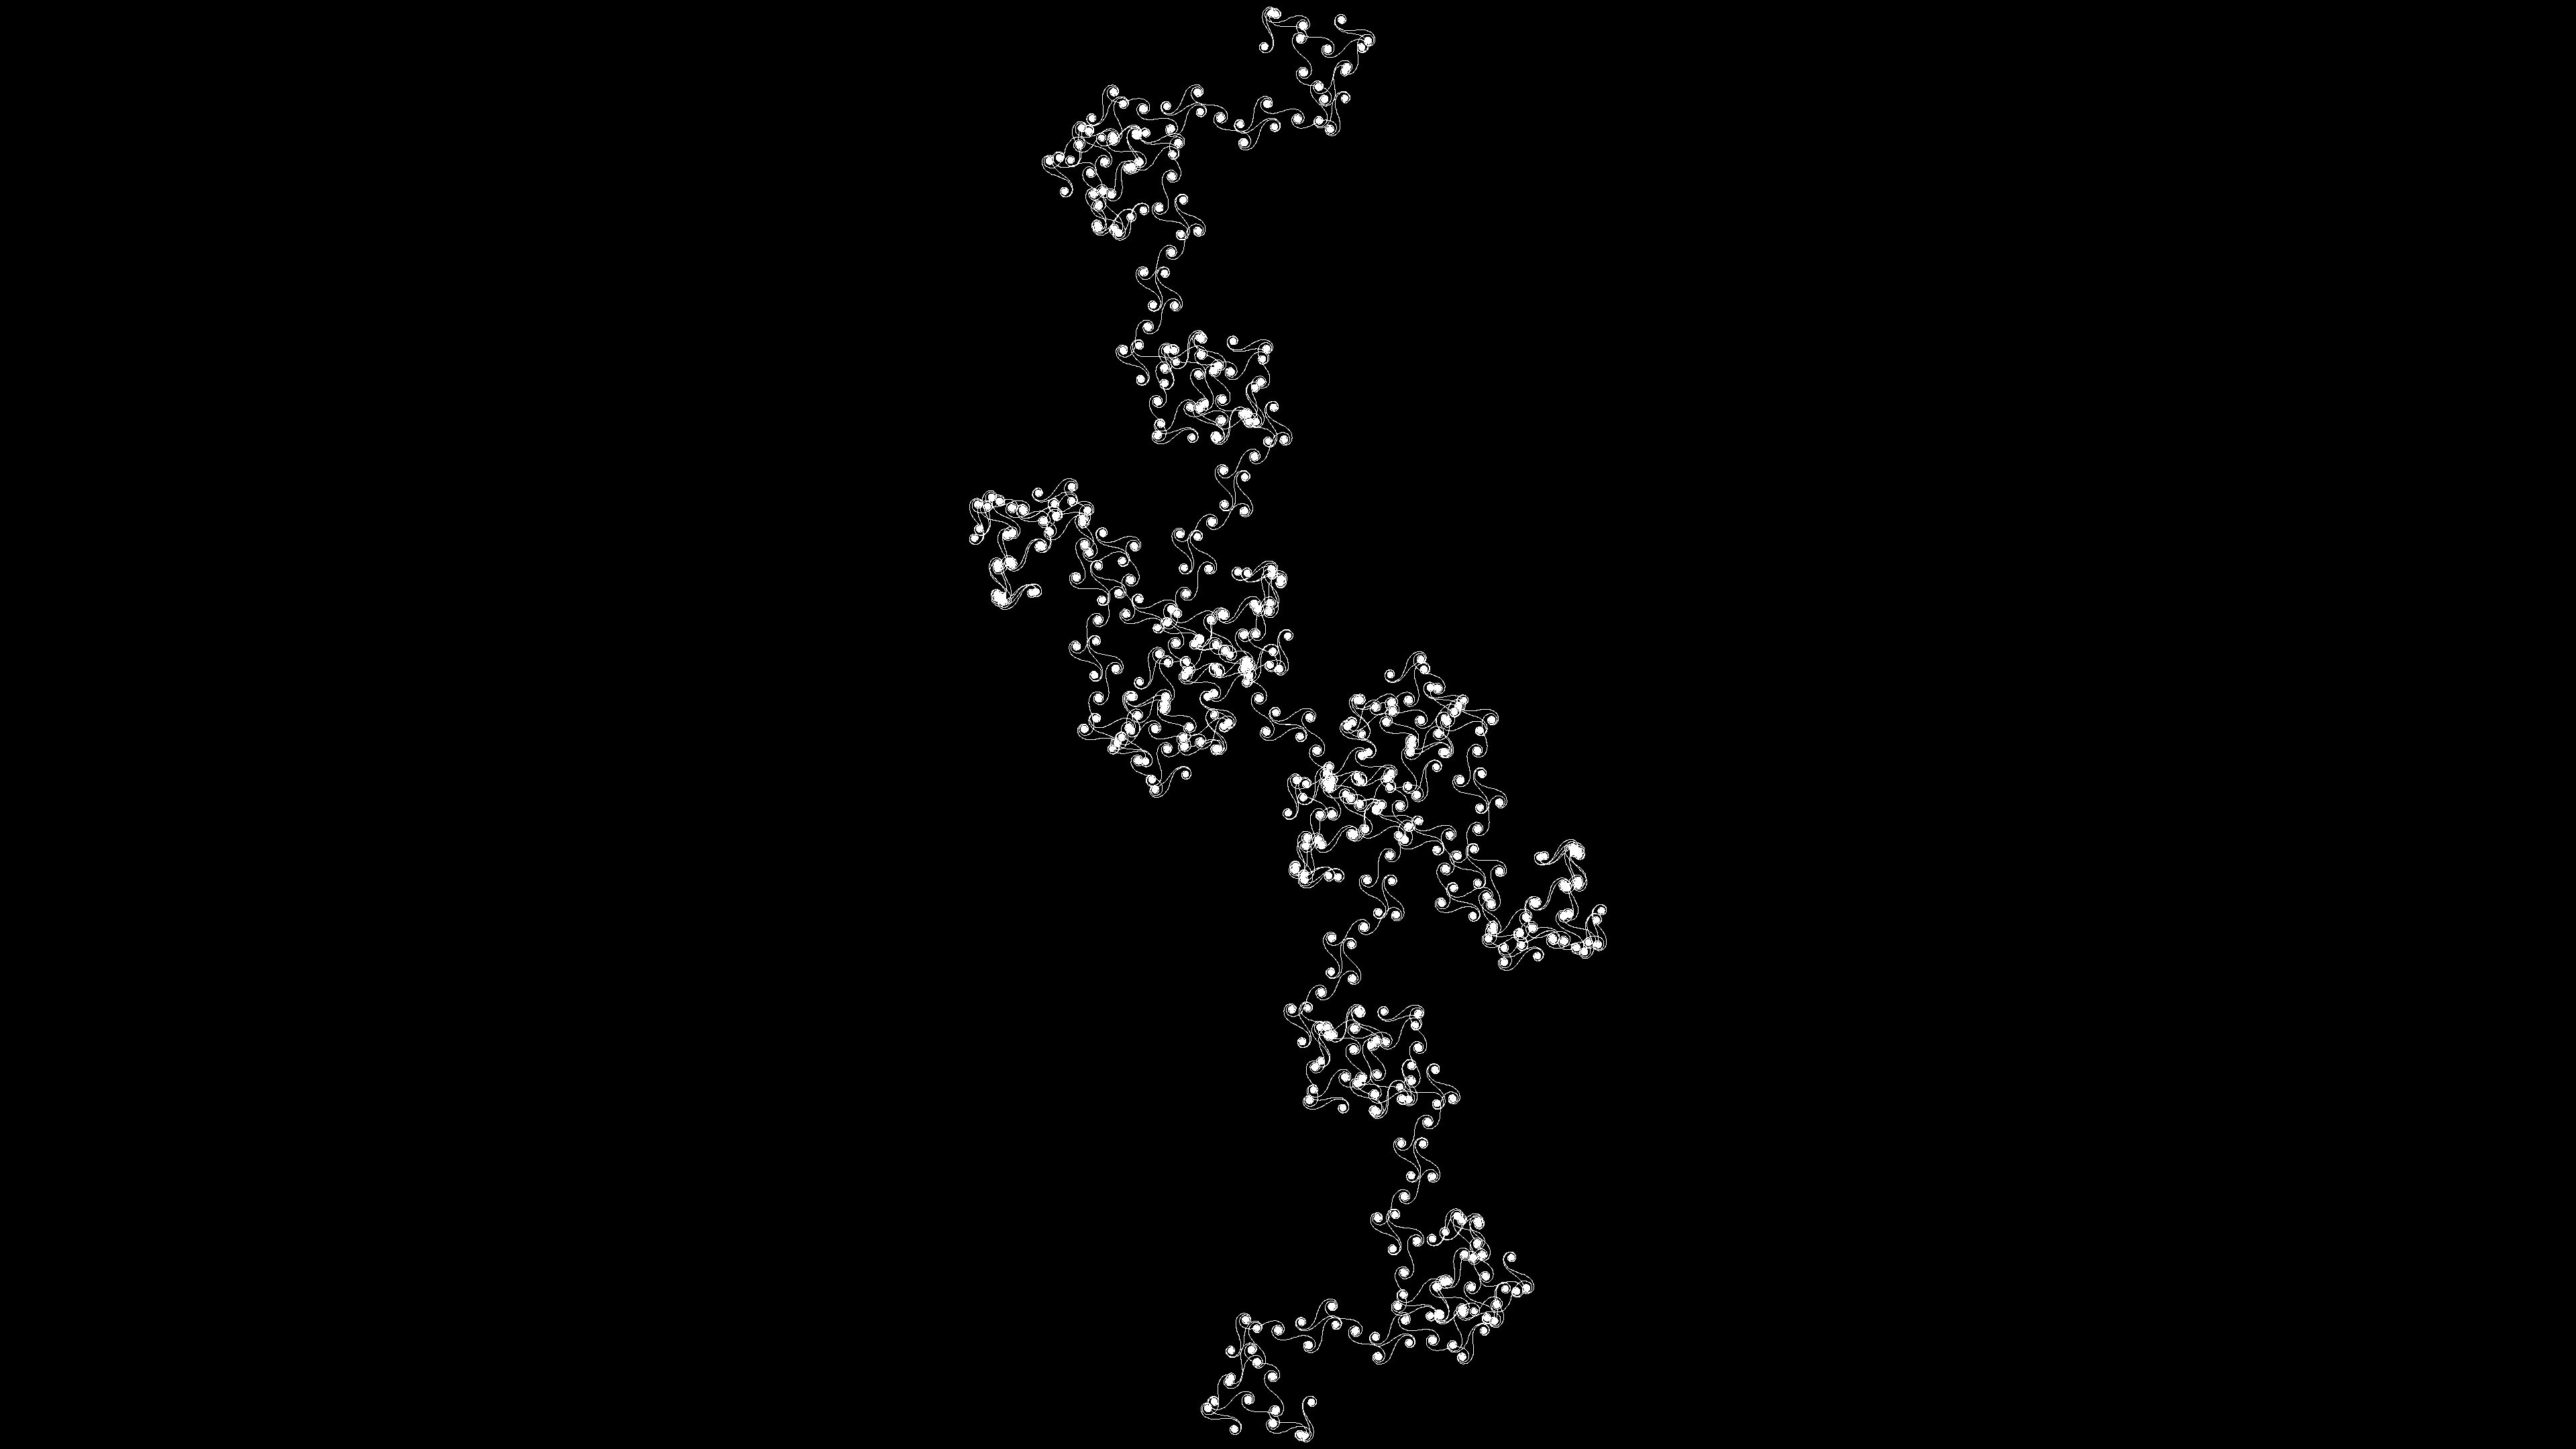
\includegraphics[width=\linewidth]{./stepsplusoneimages/0000000103.png}
    \caption{tf p=499 q=199702 theta=000 89954032.png}
  \end{subfigure}
  \begin{subfigure}[t]{0.48\textwidth}
    \centering
    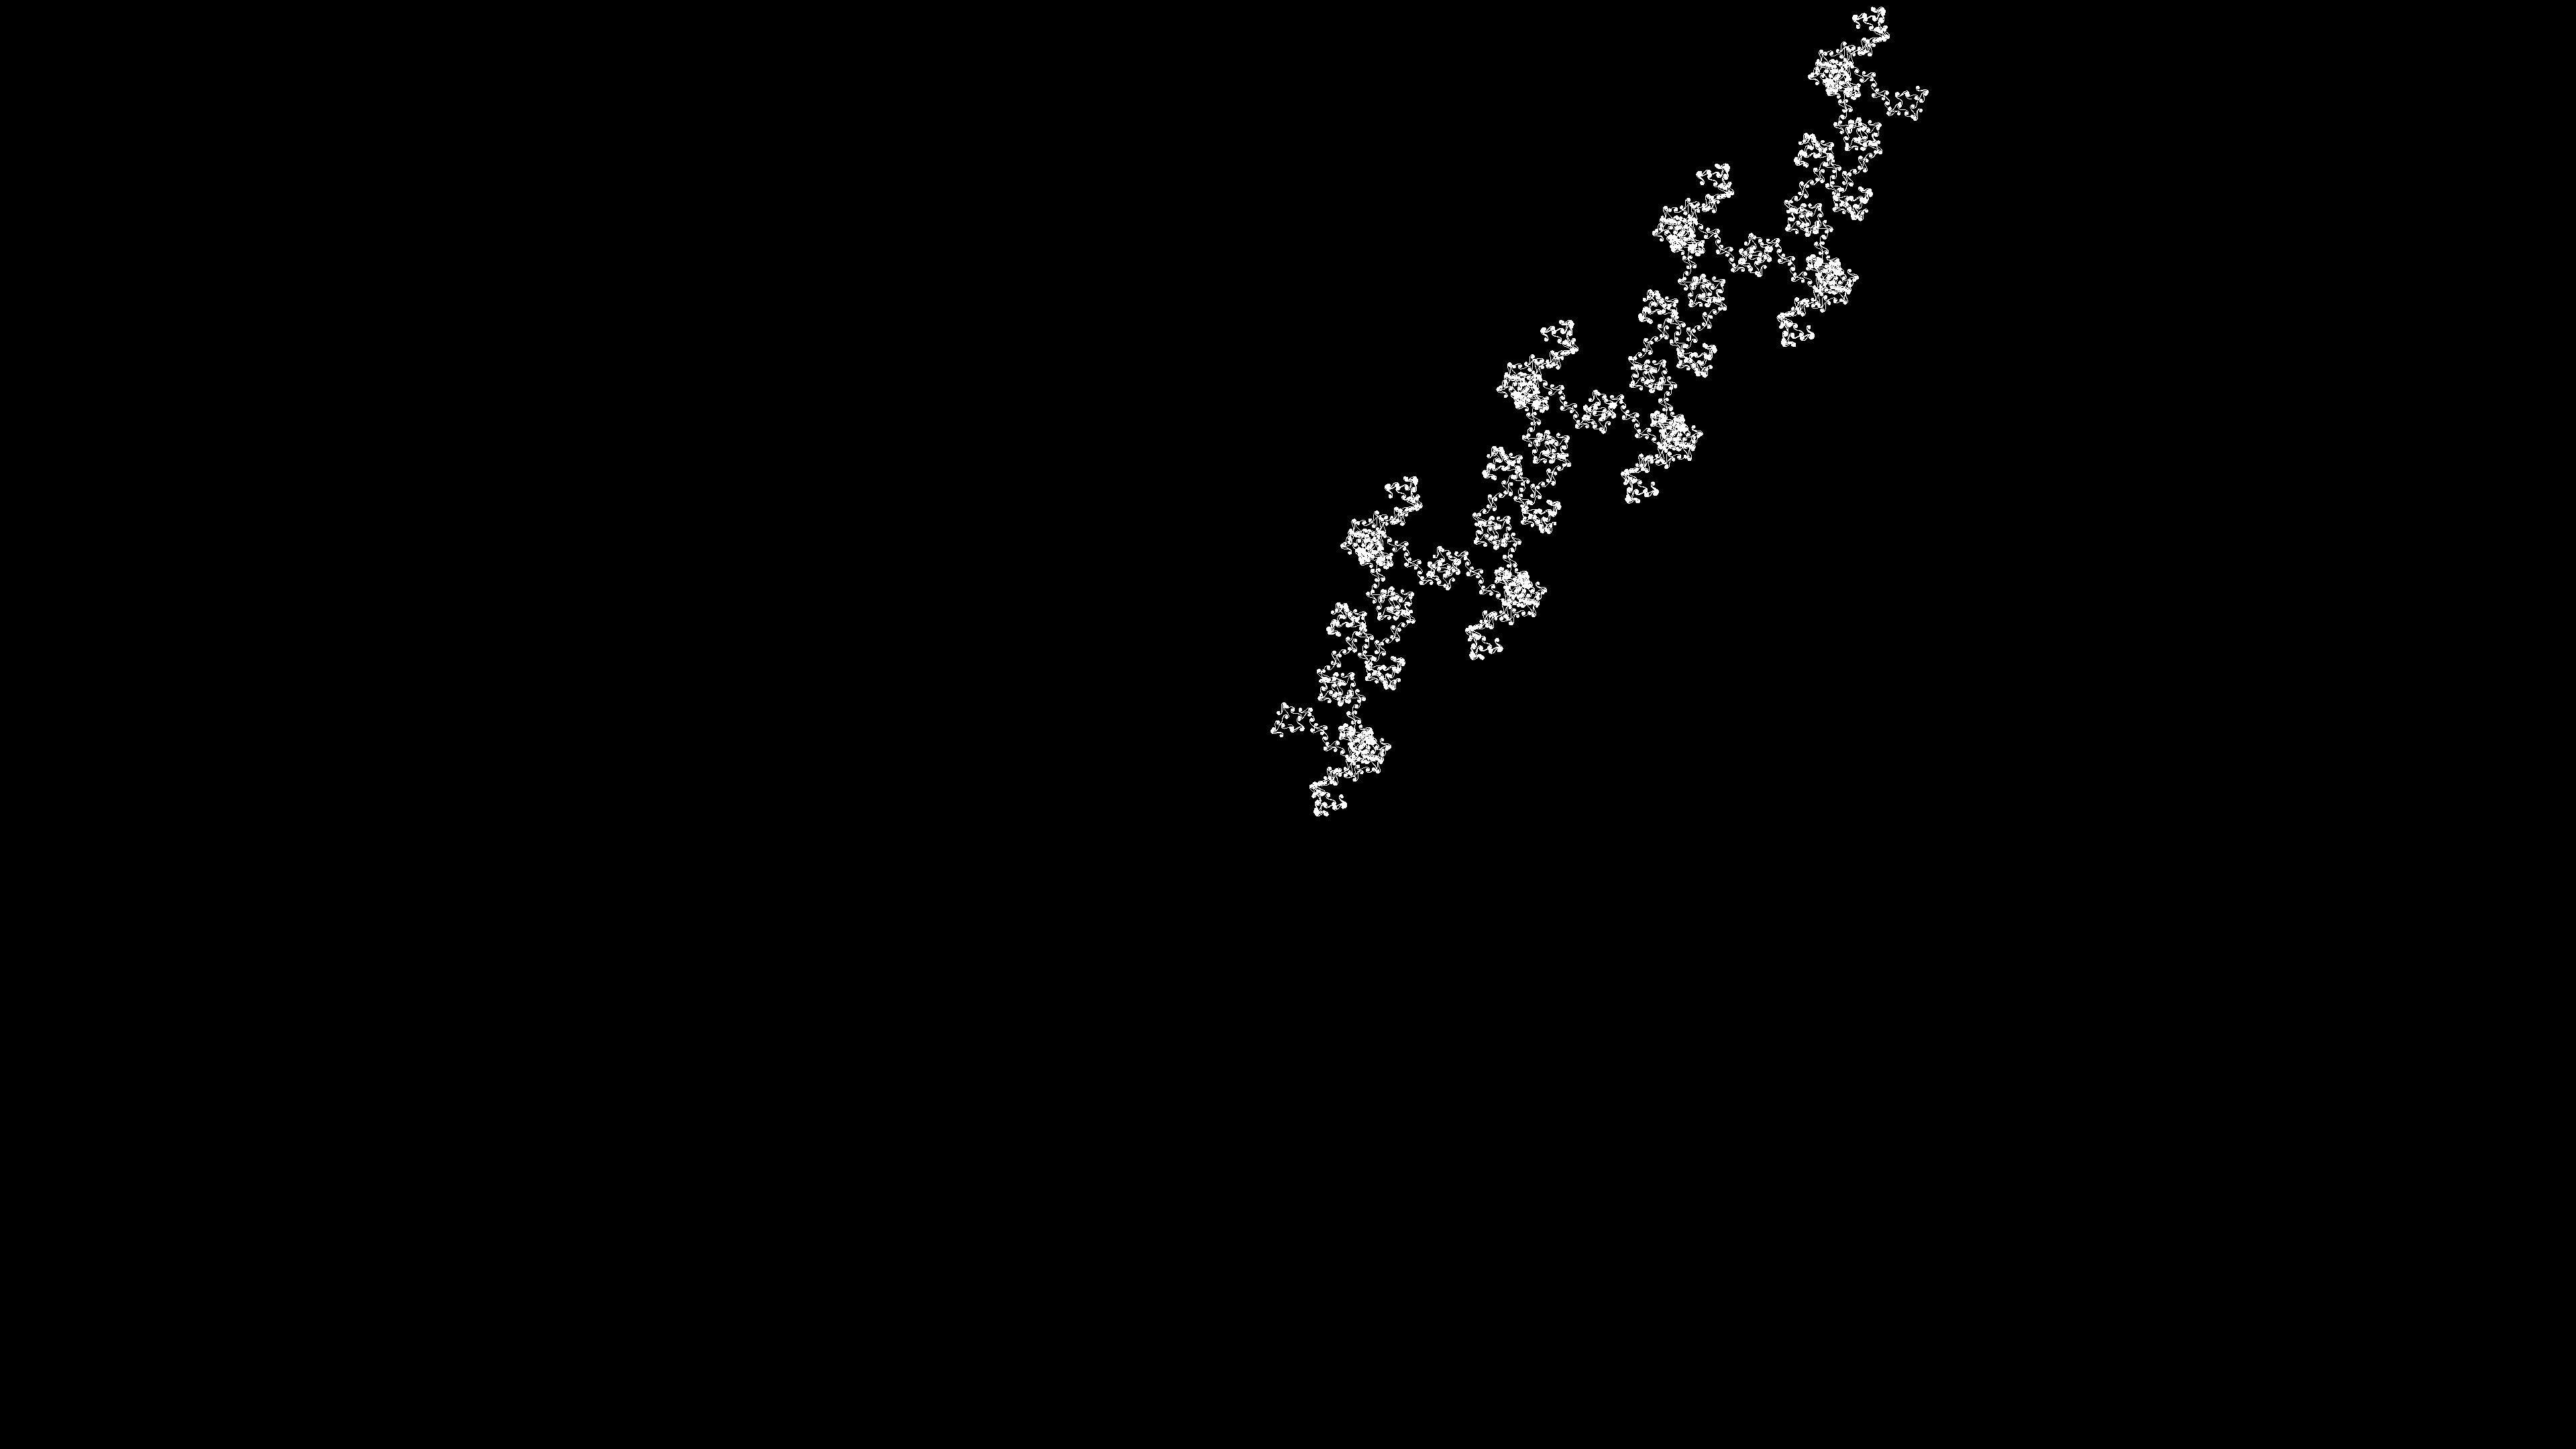
\includegraphics[width=\linewidth]{./stepsplusoneimages/0000000104.png}
    \caption{tf p=499 q=200201 theta=000 89729822.png}
  \end{subfigure}
  \caption{n=102 s=400 s+1=401}
  \label{fig:n=102}
\end{figure}
\begin{figure}[H]
  \centering
  \begin{subfigure}[t]{0.48\textwidth}
    \centering
    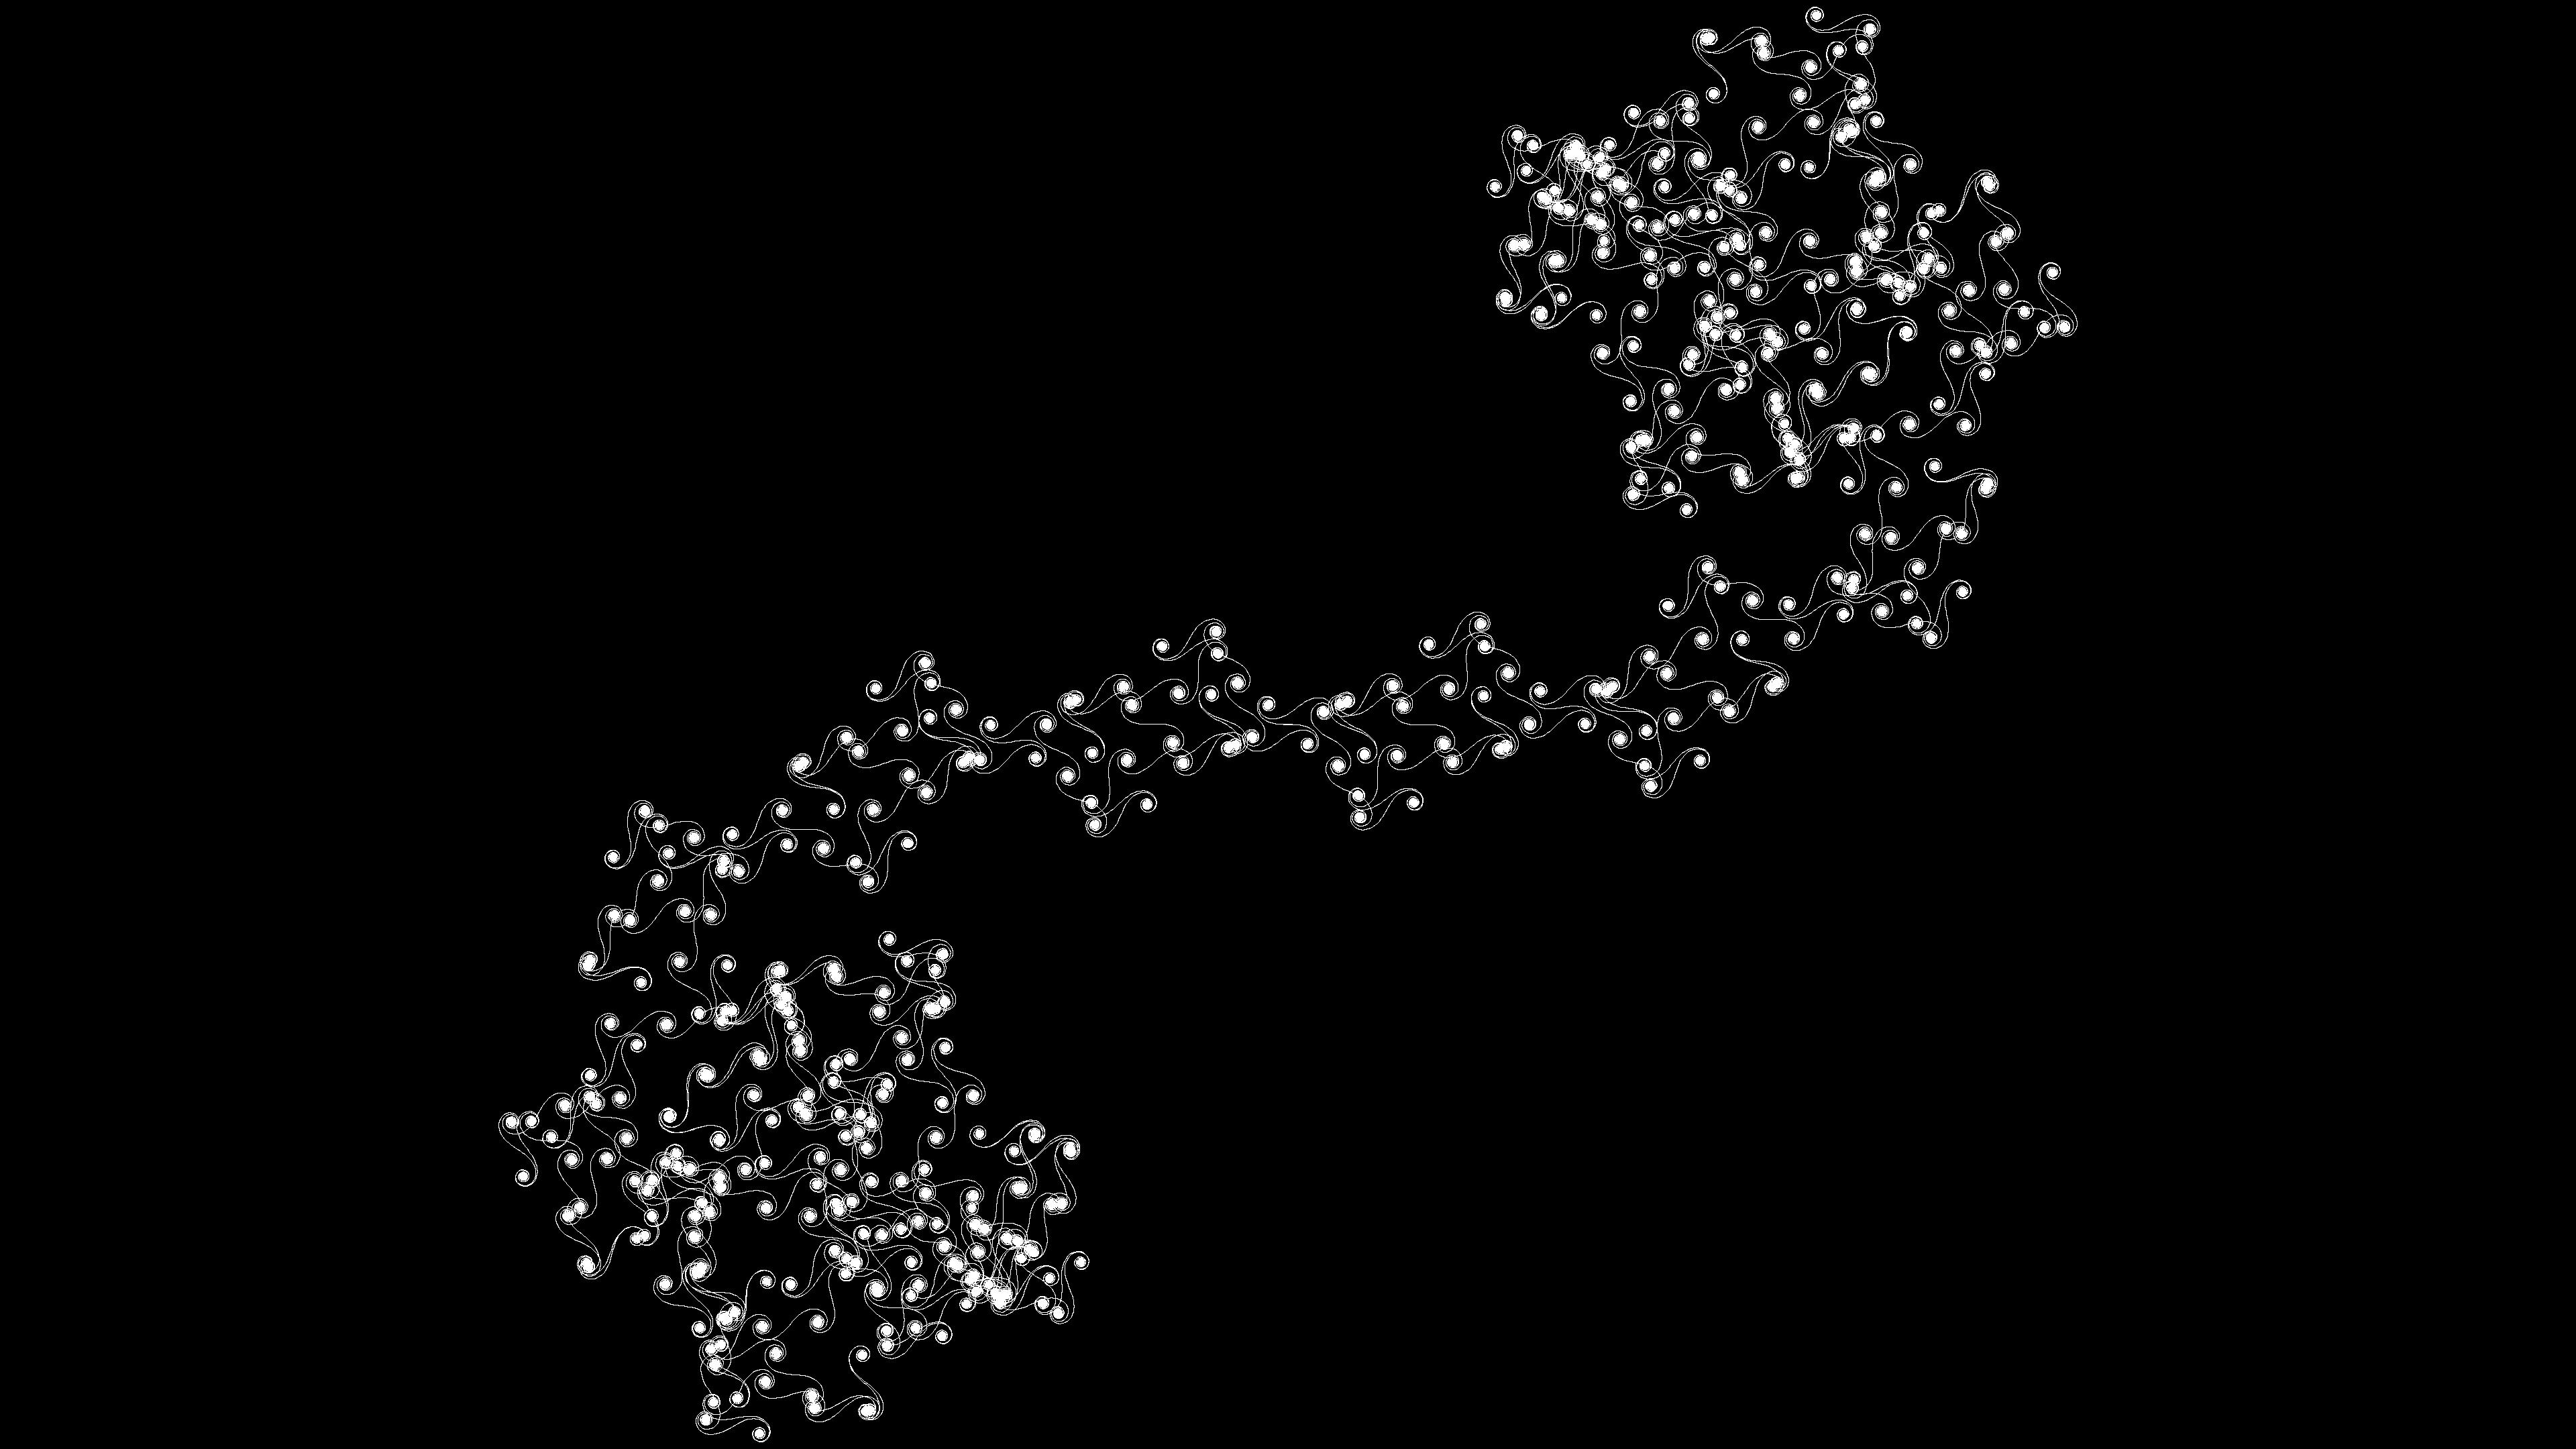
\includegraphics[width=\linewidth]{./stepsplusoneimages/0000000105.png}
    \caption{tf p=499 q=199704 theta=000 89953131.png}
  \end{subfigure}
  \begin{subfigure}[t]{0.48\textwidth}
    \centering
    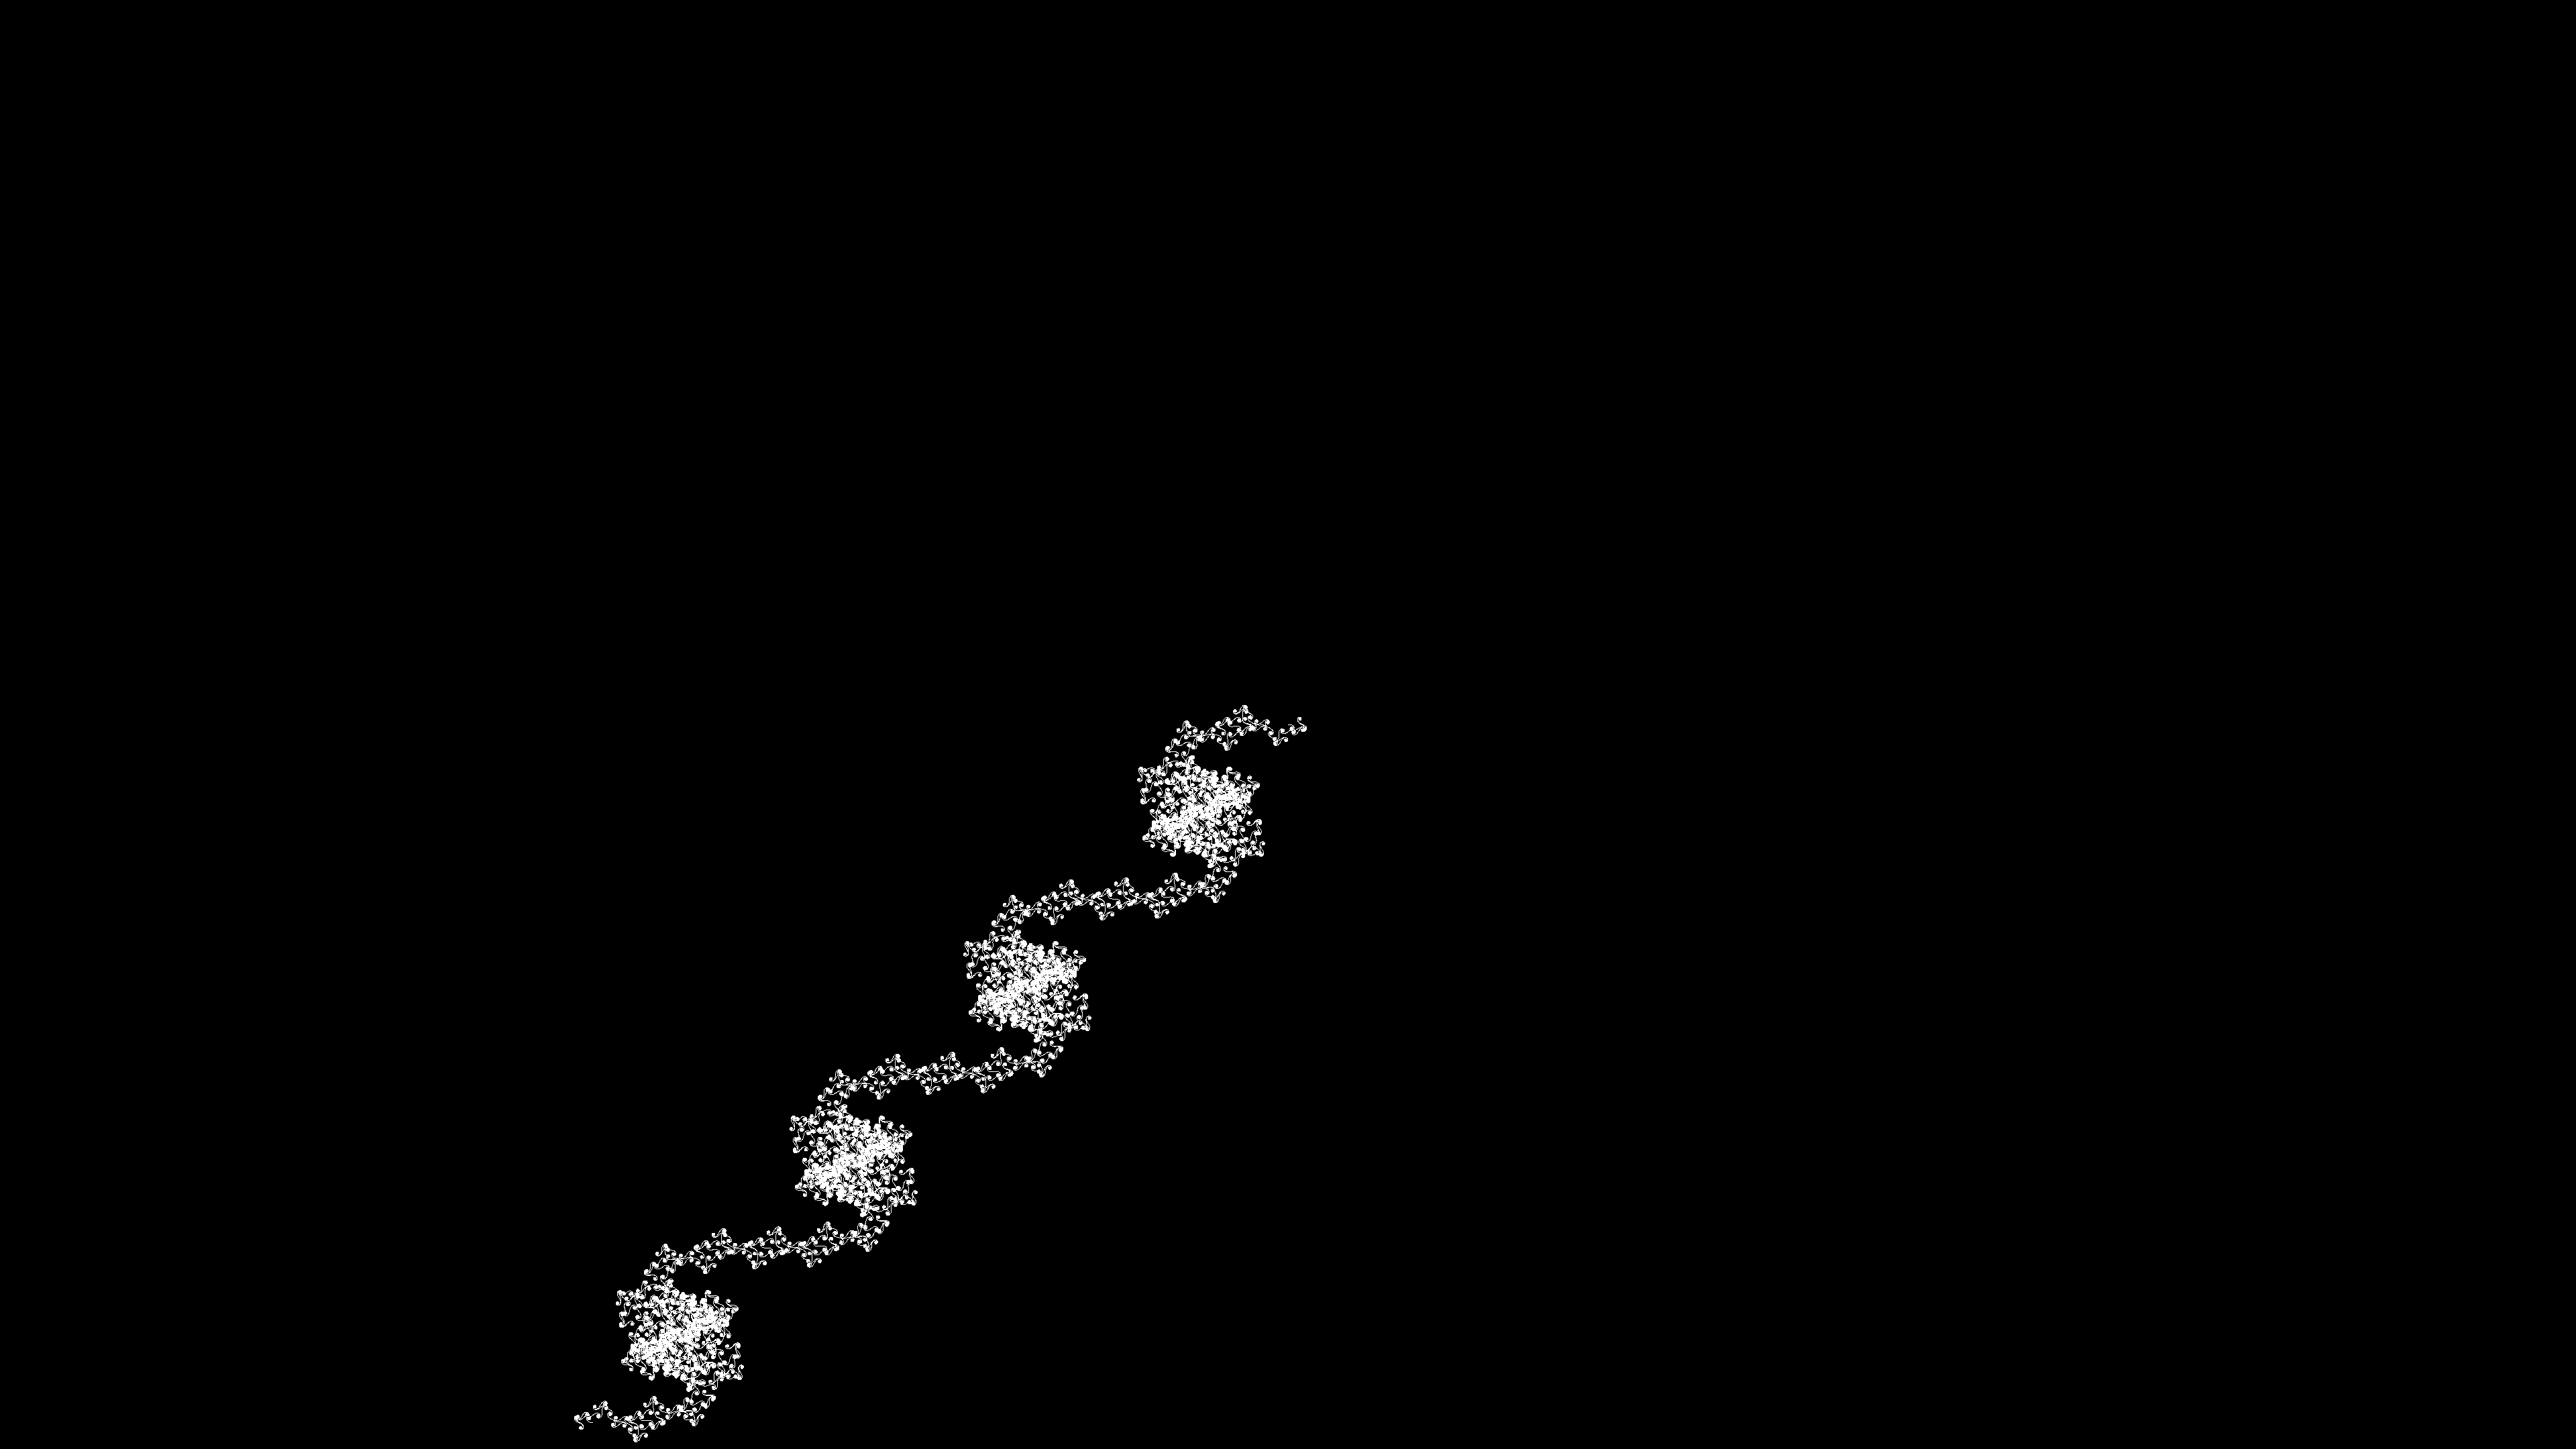
\includegraphics[width=\linewidth]{./stepsplusoneimages/0000000106.png}
    \caption{tf p=499 q=200203 theta=000 89728925.png}
  \end{subfigure}
  \caption{n=104 s=400 s+1=401}
  \label{fig:n=104}
\end{figure}
\begin{figure}[H]
  \centering
  \begin{subfigure}[t]{0.48\textwidth}
    \centering
    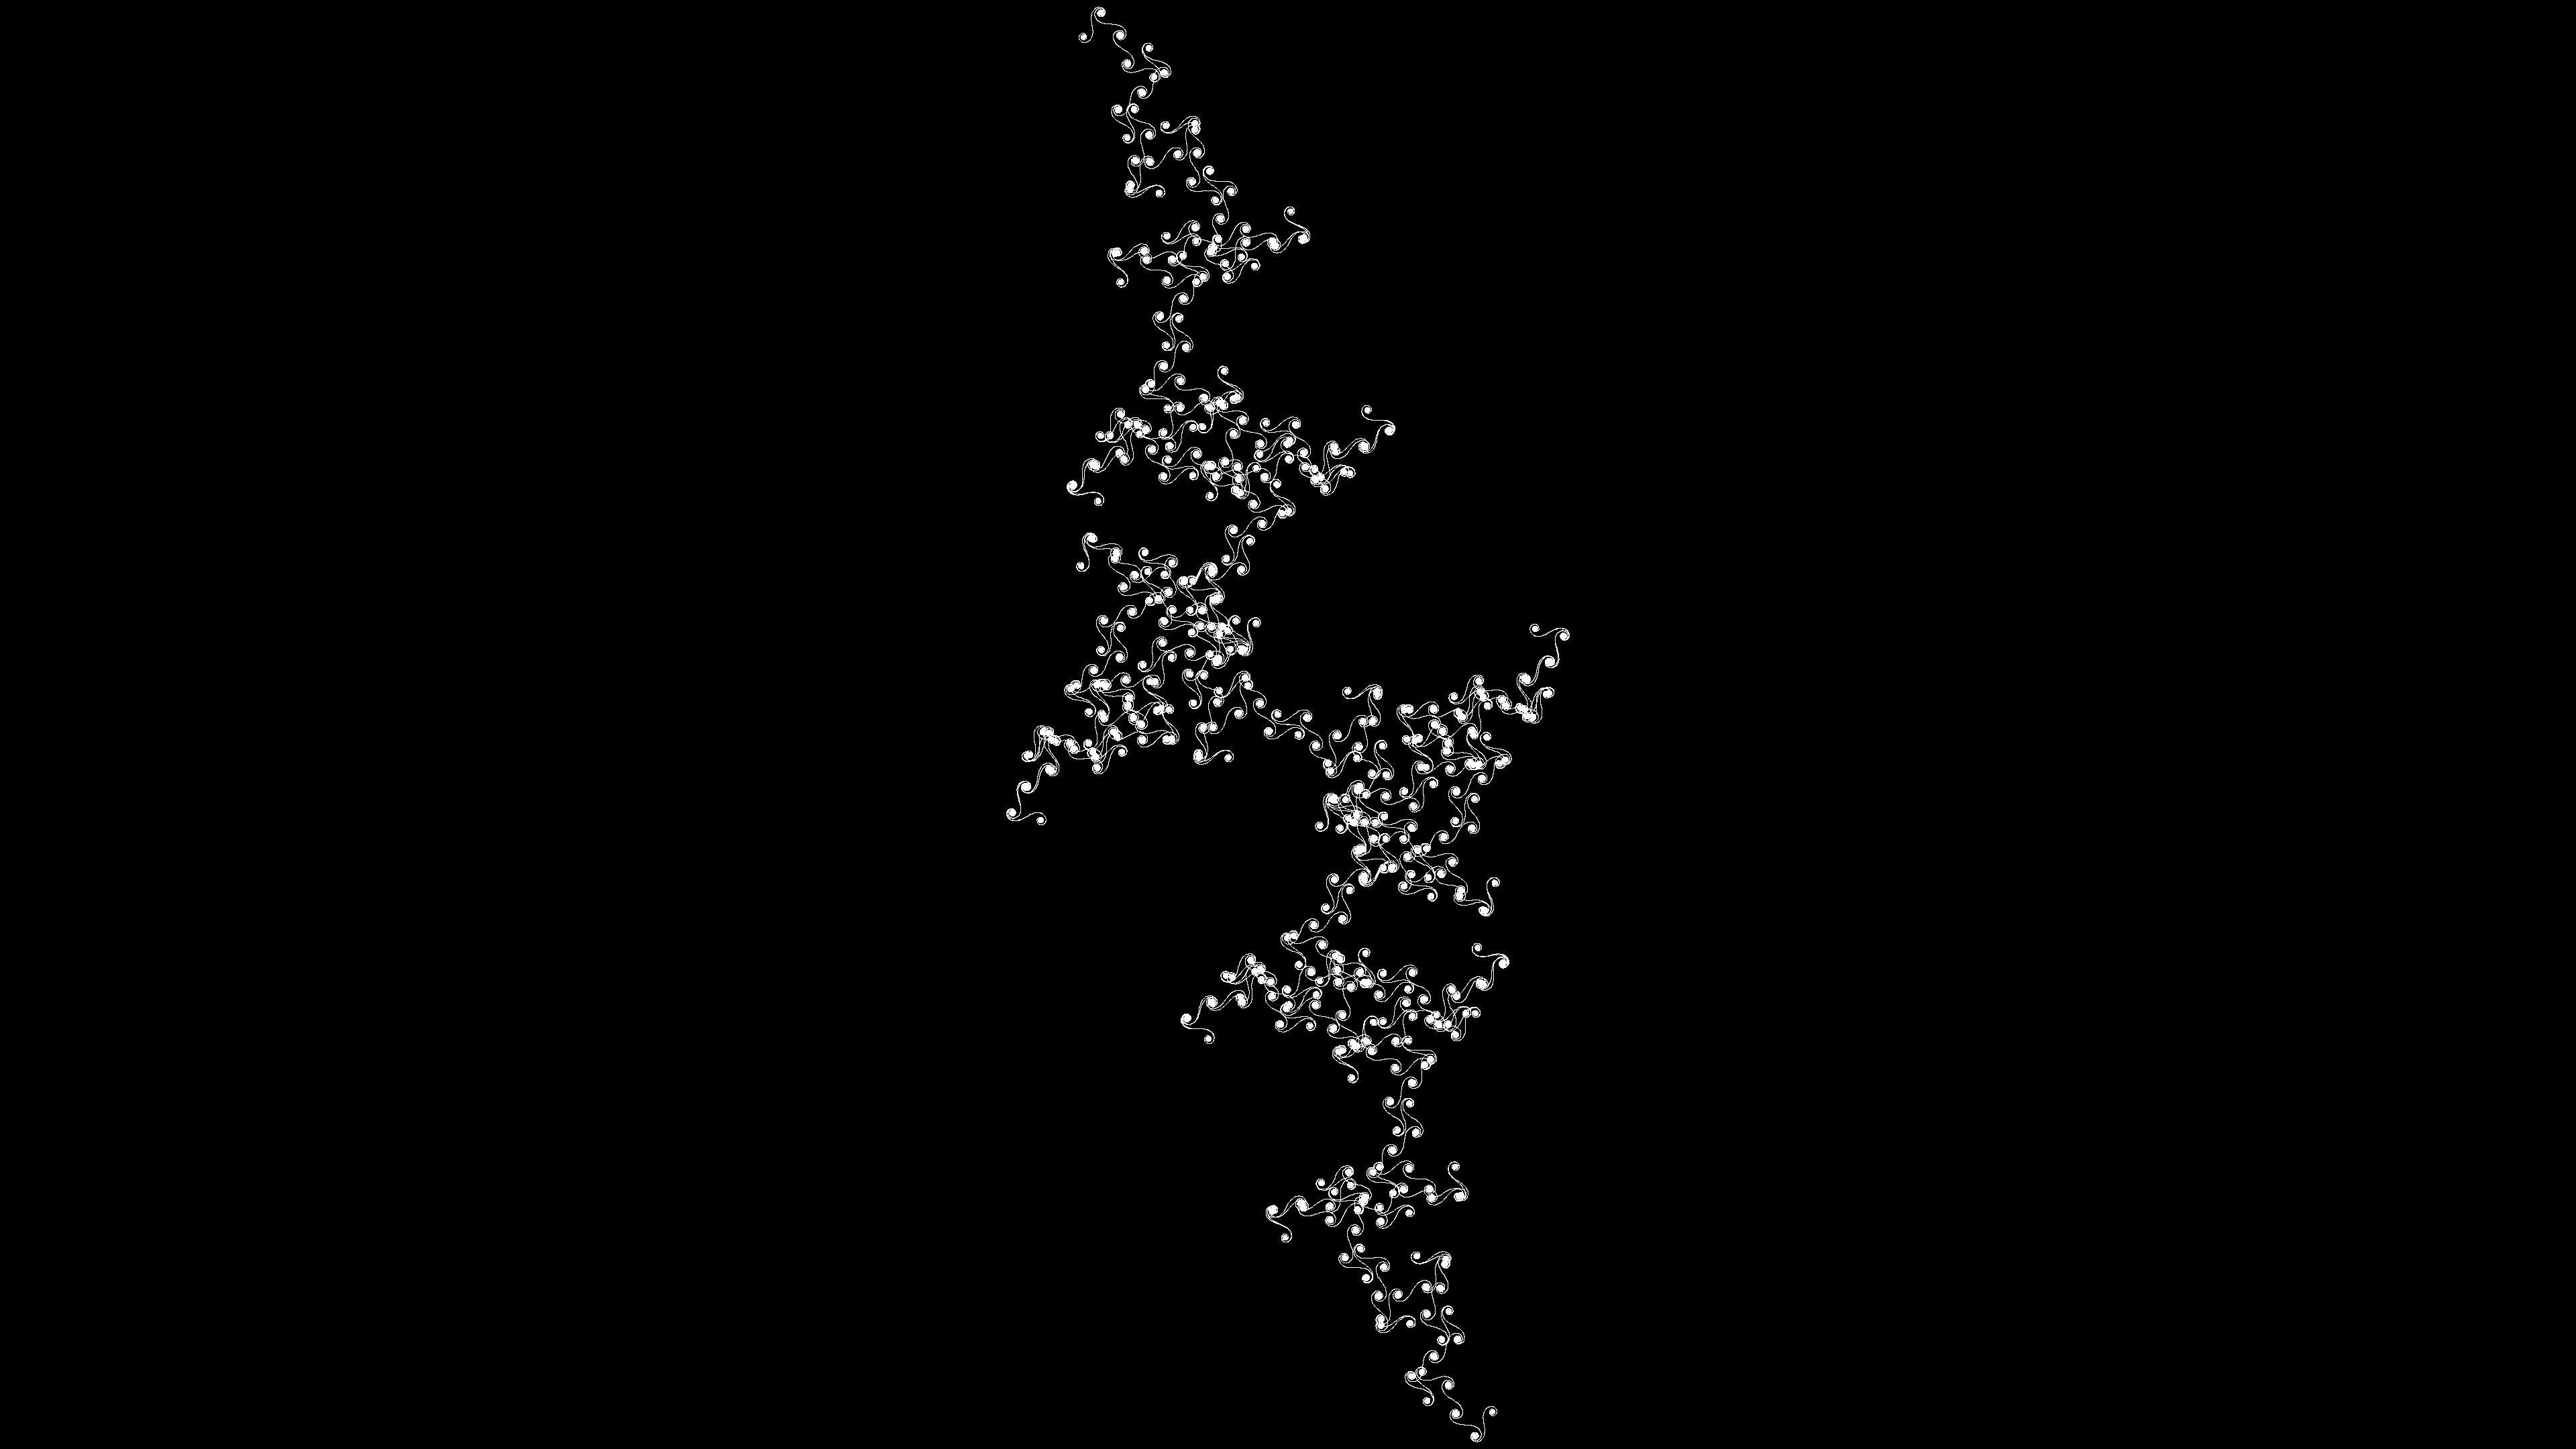
\includegraphics[width=\linewidth]{./stepsplusoneimages/0000000107.png}
    \caption{tf p=499 q=199706 theta=000 89952230.png}
  \end{subfigure}
  \begin{subfigure}[t]{0.48\textwidth}
    \centering
    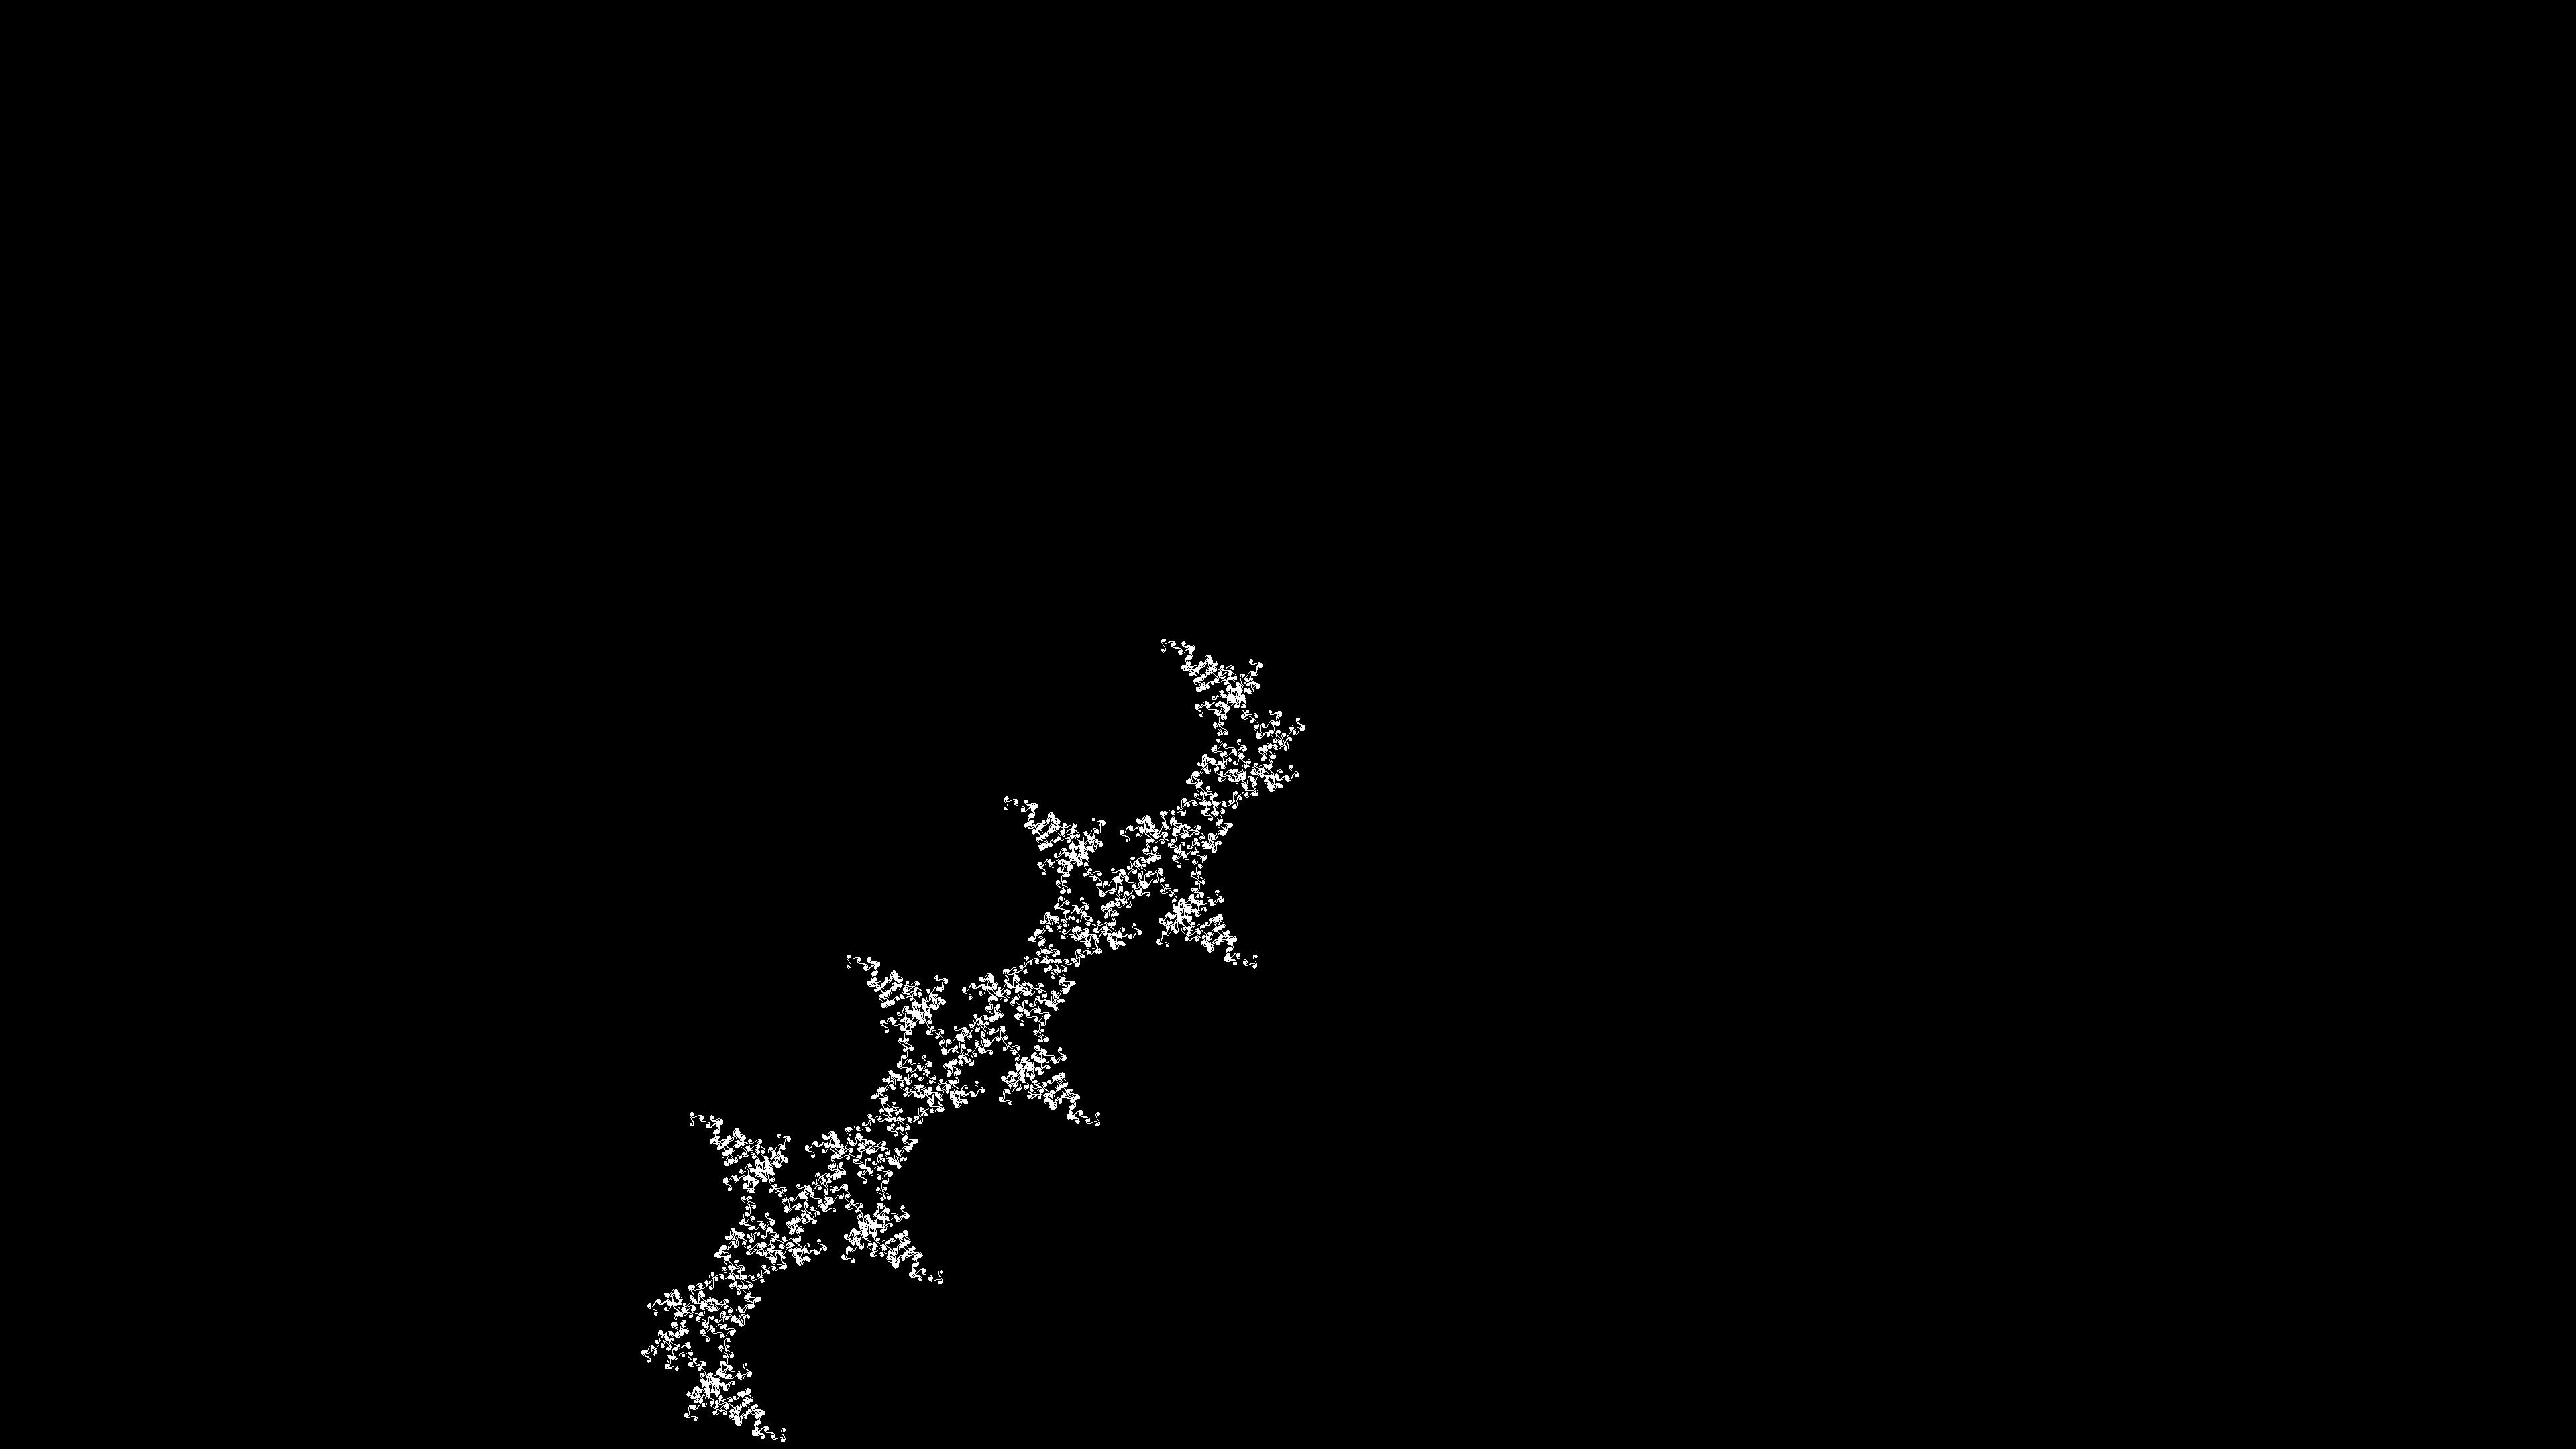
\includegraphics[width=\linewidth]{./stepsplusoneimages/0000000108.png}
    \caption{tf p=499 q=200205 theta=000 89728029.png}
  \end{subfigure}
  \caption{n=106 s=400 s+1=401}
  \label{fig:n=106}
\end{figure}
\begin{figure}[H]
  \centering
  \begin{subfigure}[t]{0.48\textwidth}
    \centering
    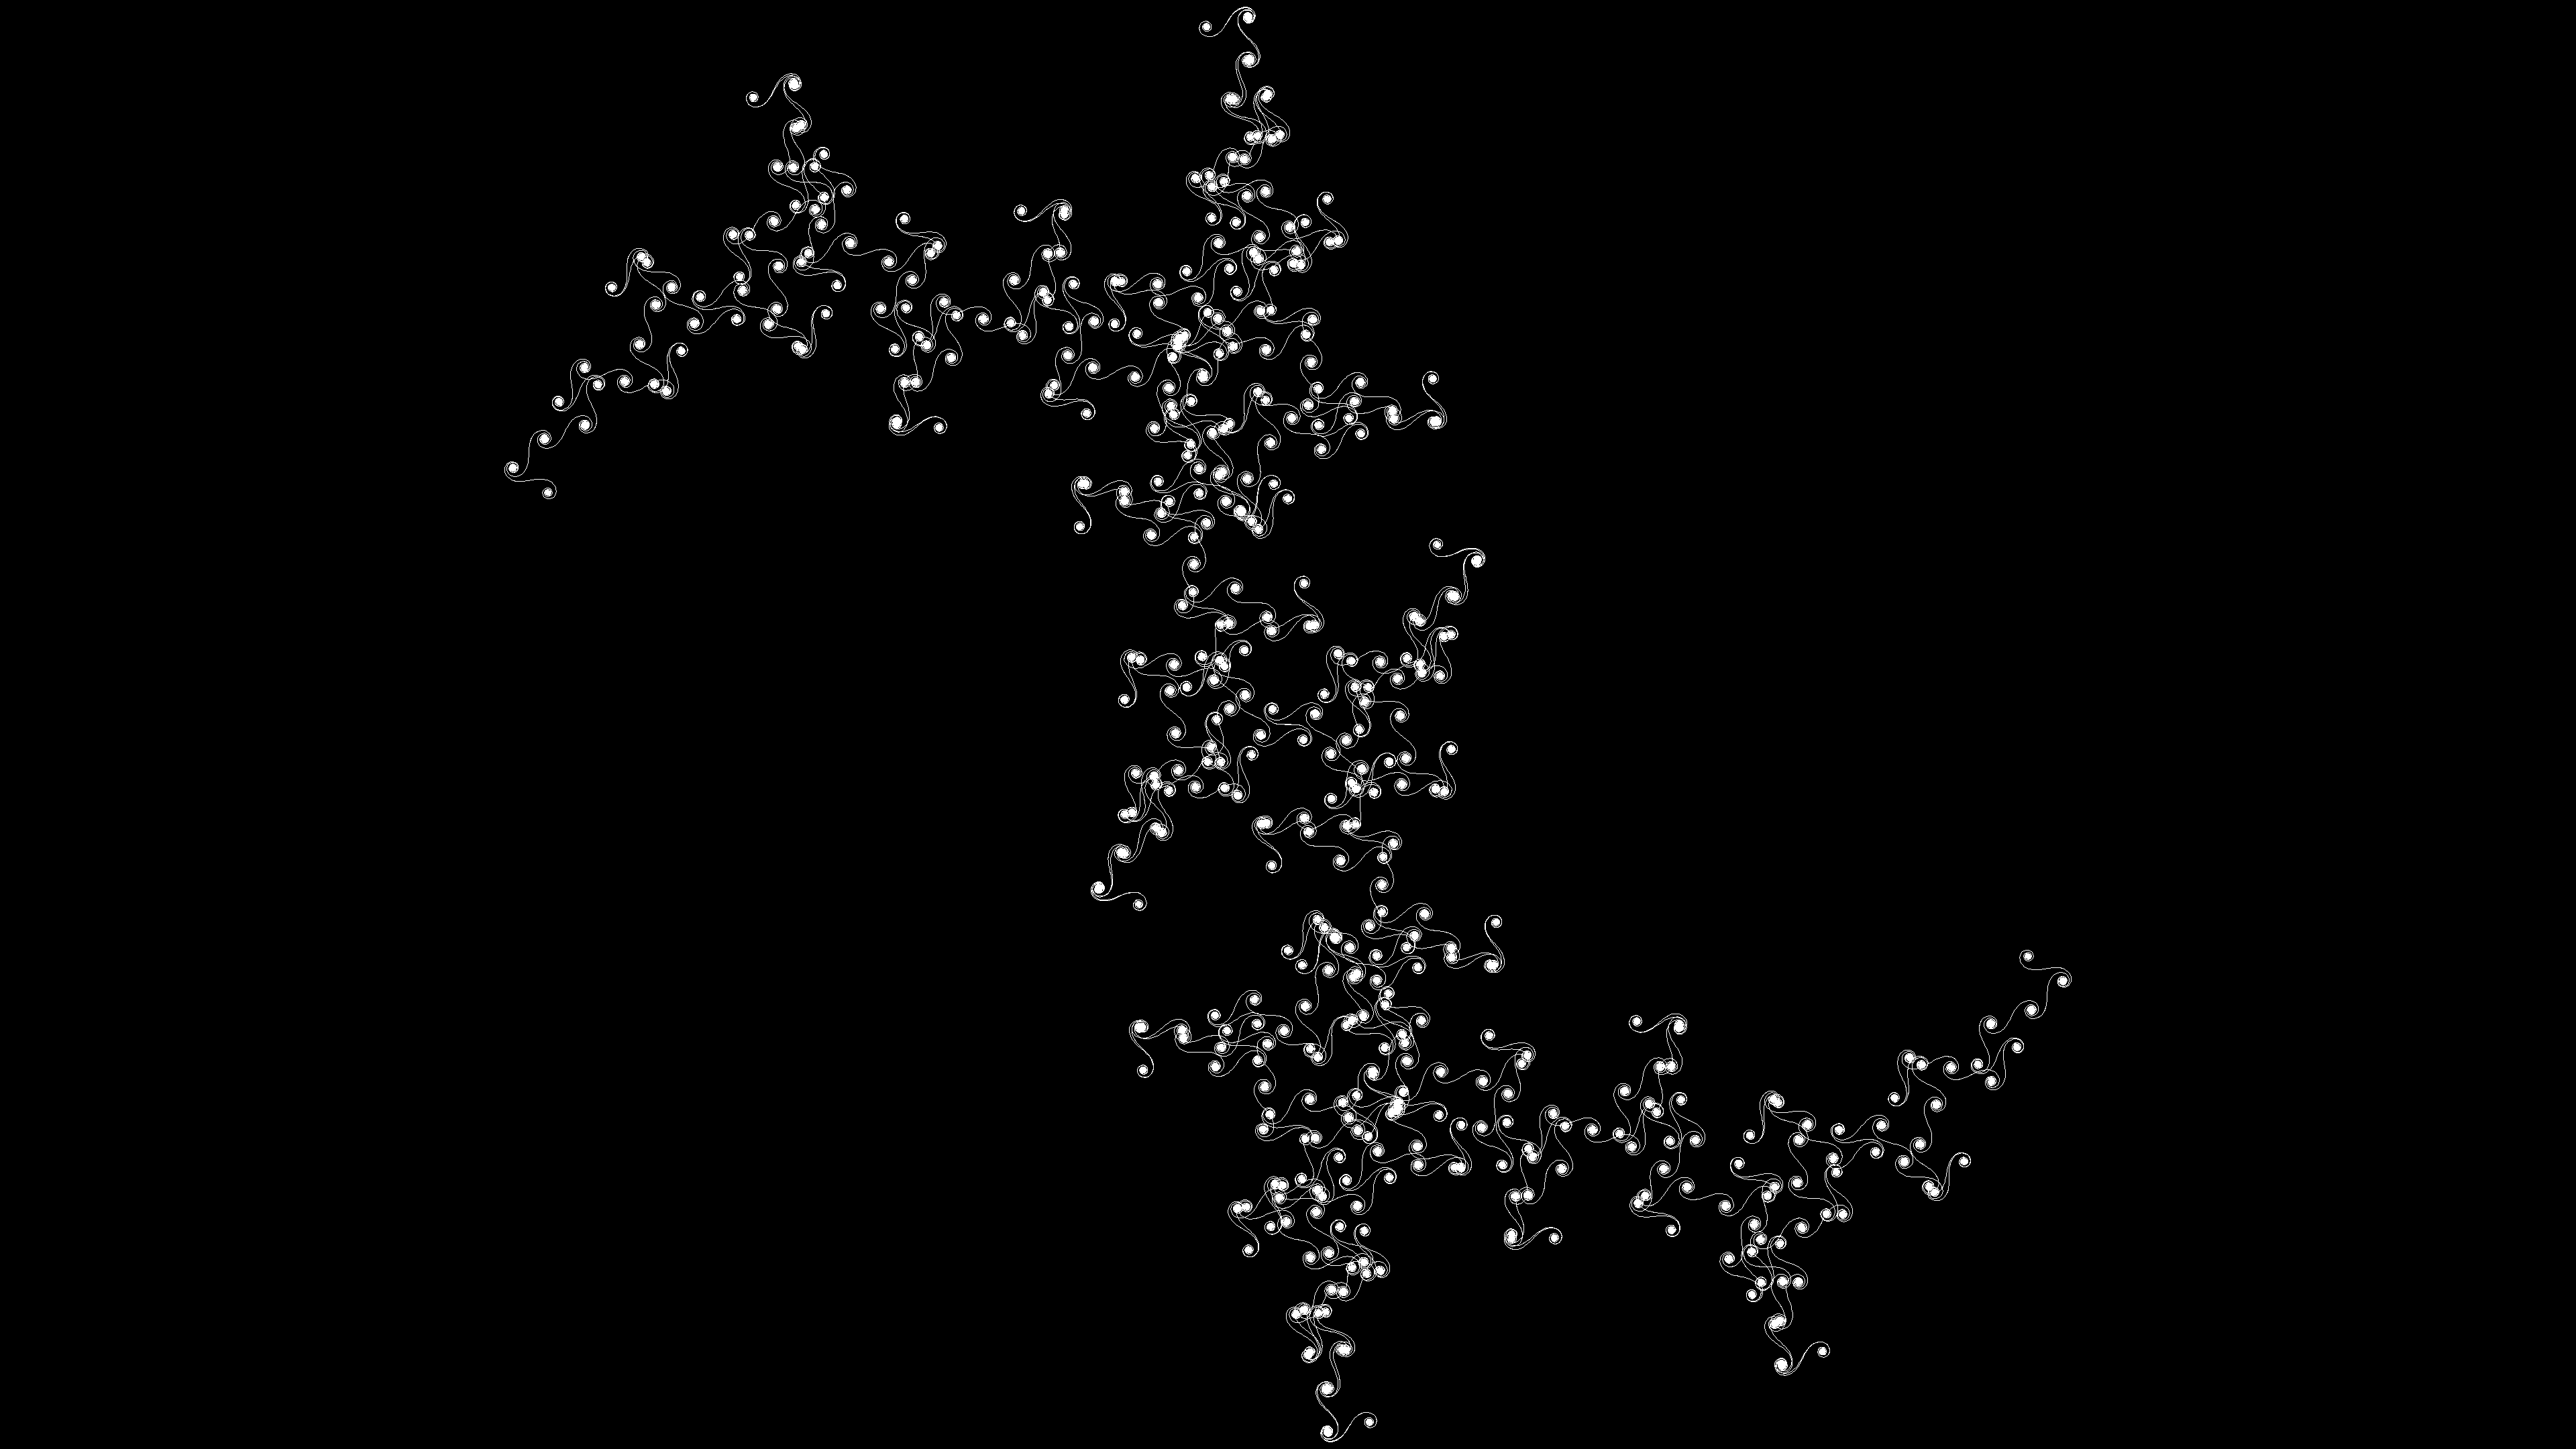
\includegraphics[width=\linewidth]{./stepsplusoneimages/0000000109.png}
    \caption{tf p=499 q=199708 theta=000 89951329.png}
  \end{subfigure}
  \begin{subfigure}[t]{0.48\textwidth}
    \centering
    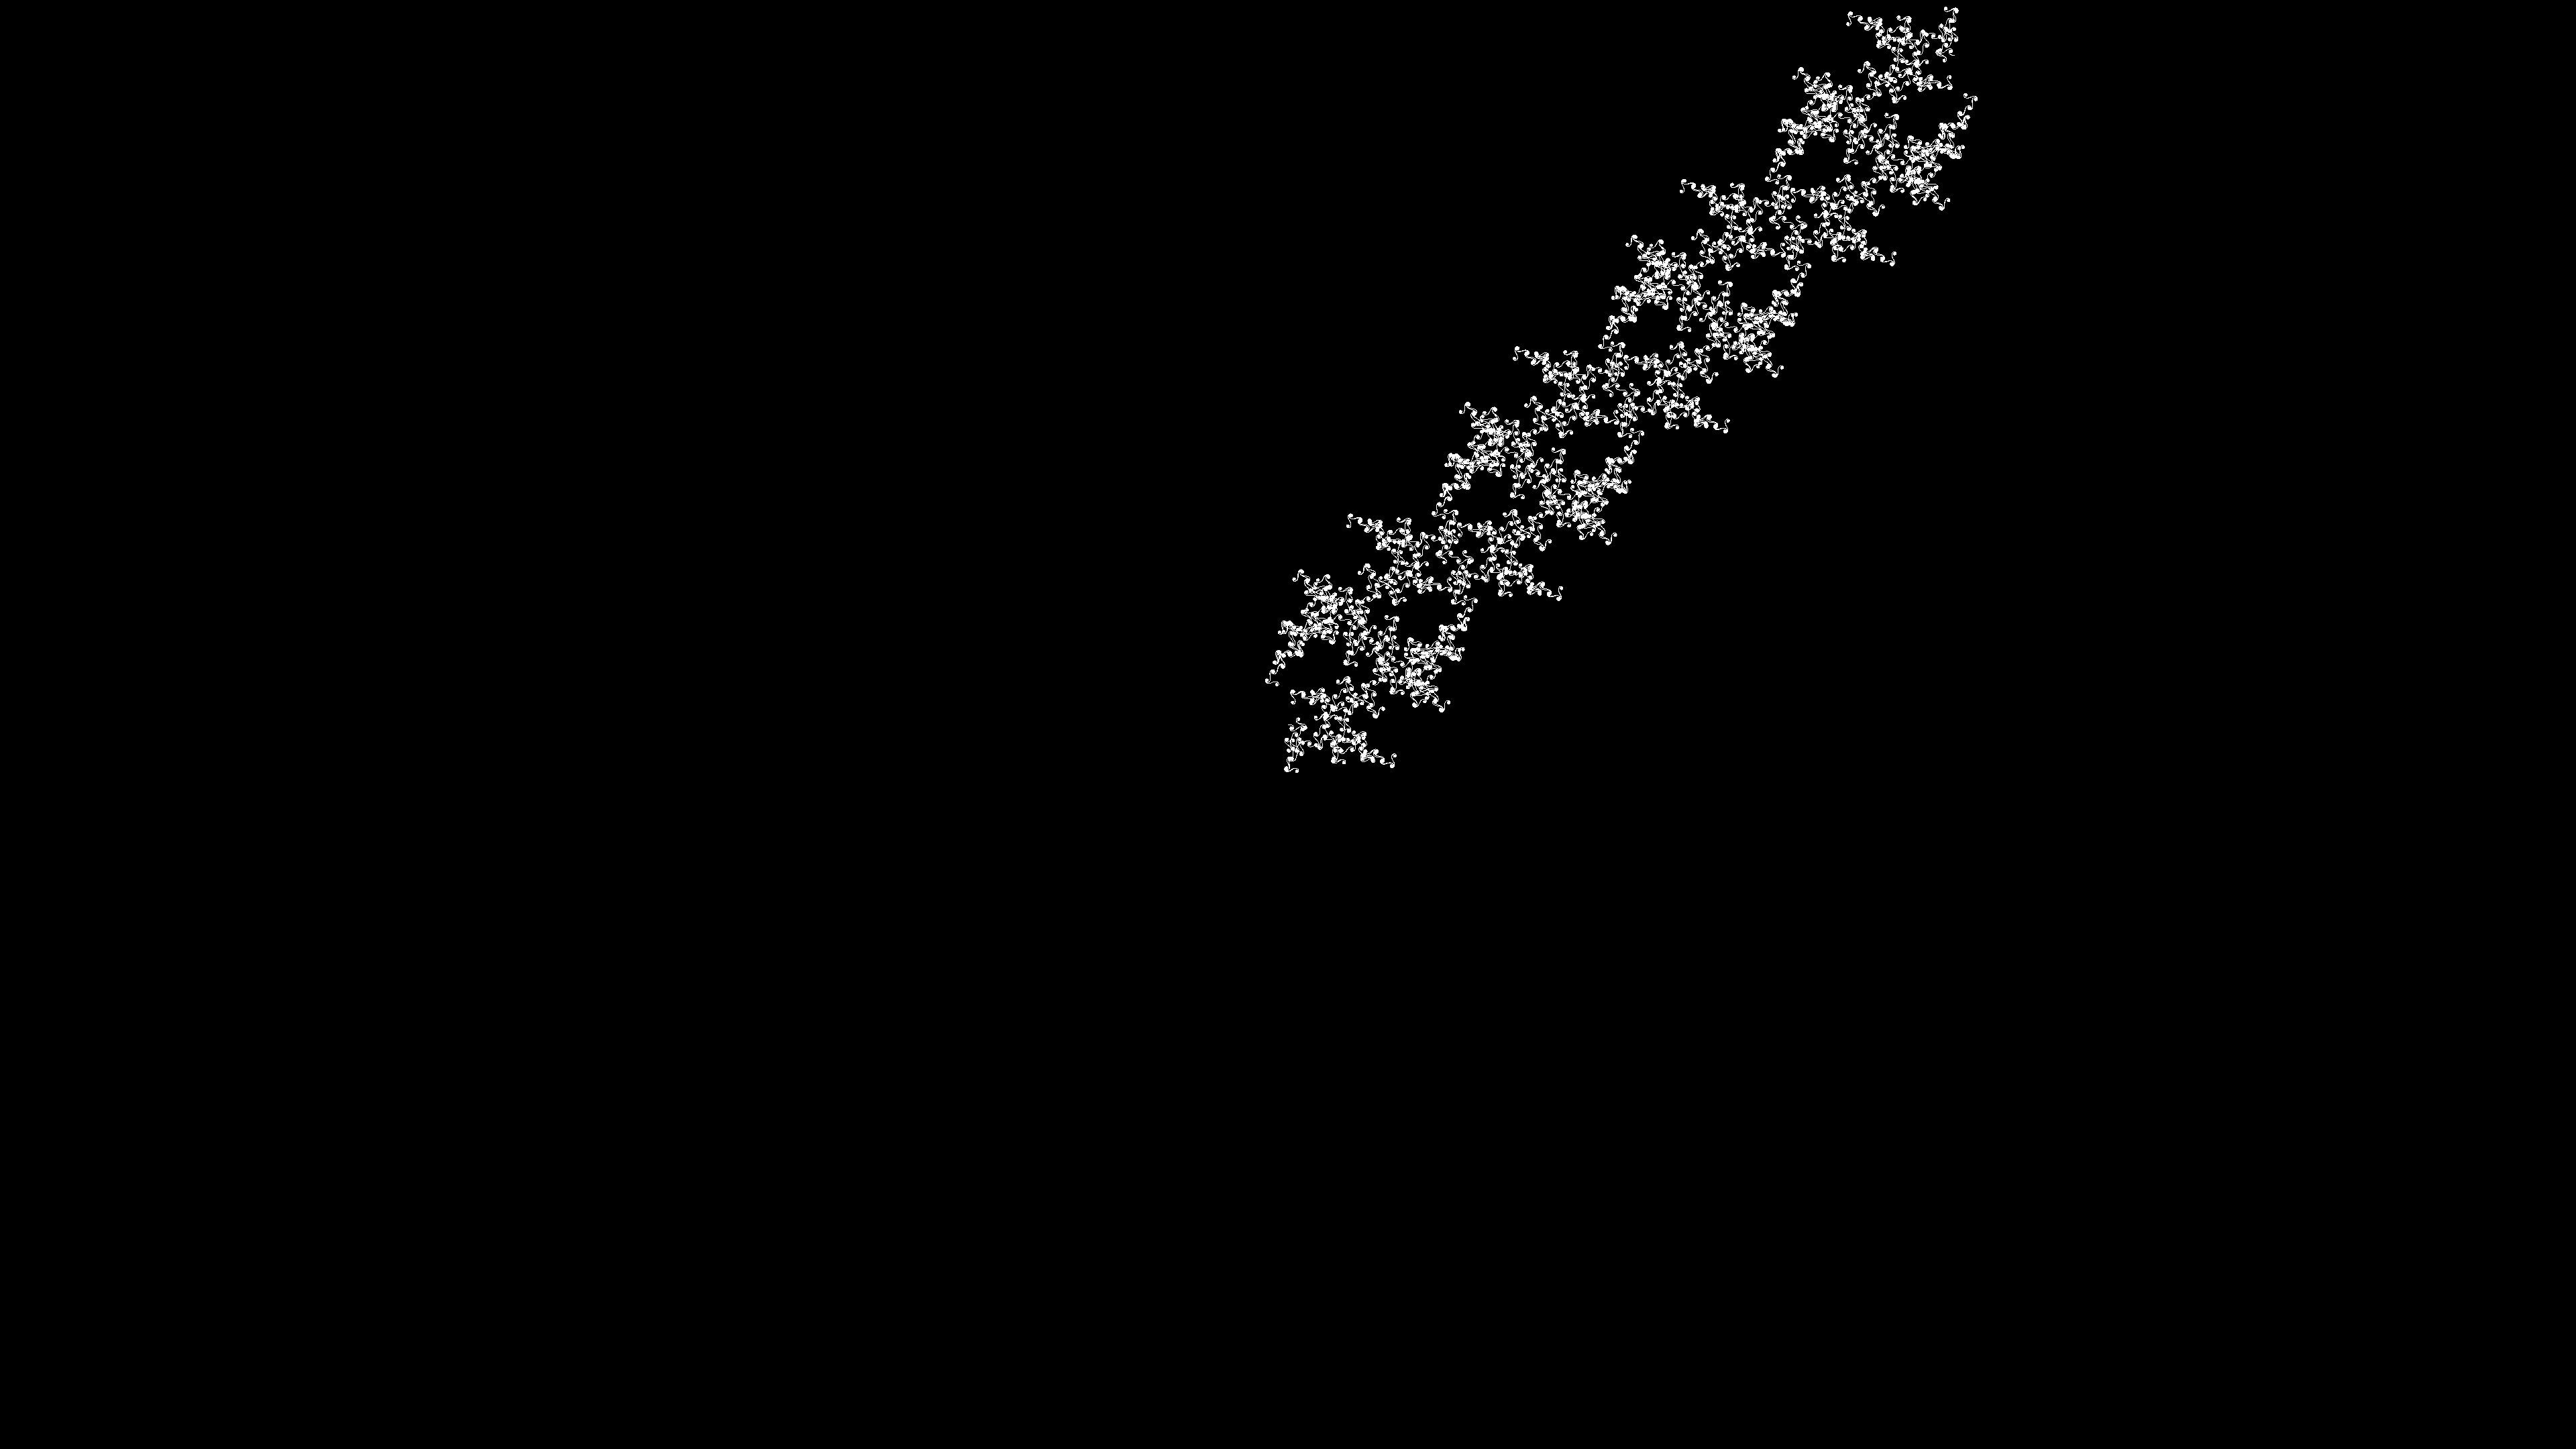
\includegraphics[width=\linewidth]{./stepsplusoneimages/0000000110.png}
    \caption{tf p=499 q=200207 theta=000 89727132.png}
  \end{subfigure}
  \caption{n=108 s=400 s+1=401}
  \label{fig:n=108}
\end{figure}
\begin{figure}[H]
  \centering
  \begin{subfigure}[t]{0.48\textwidth}
    \centering
    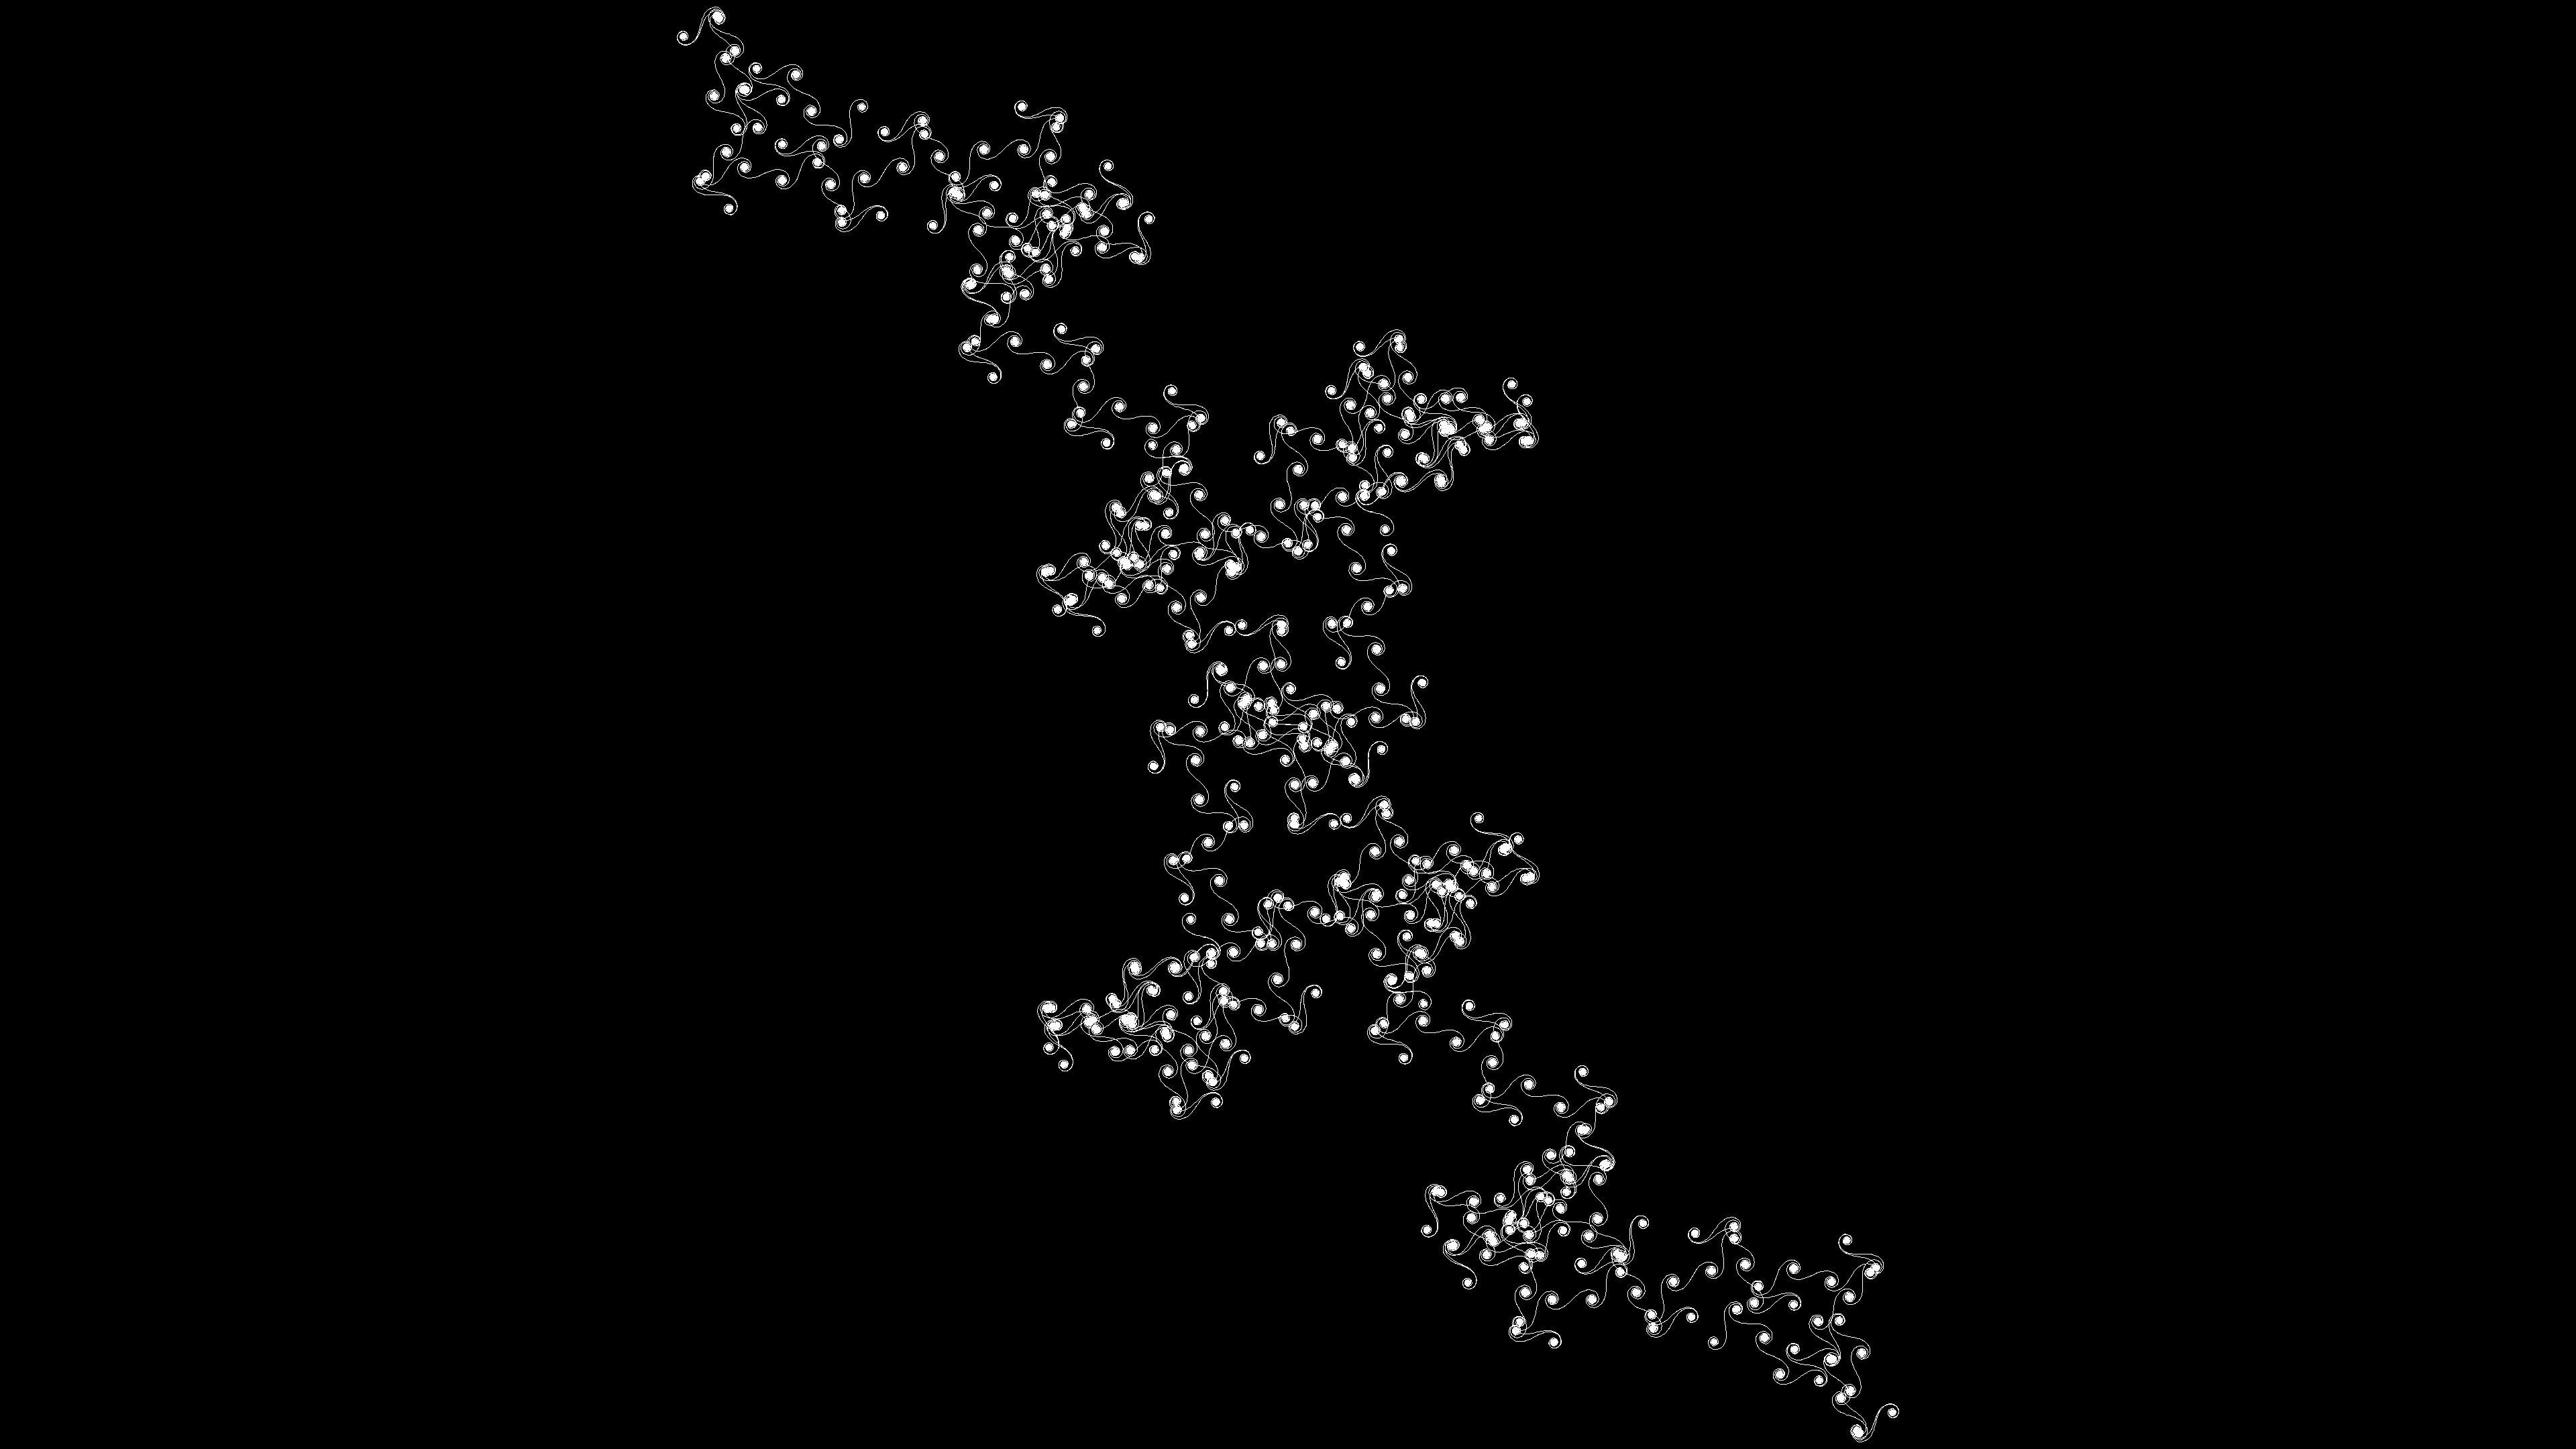
\includegraphics[width=\linewidth]{./stepsplusoneimages/0000000111.png}
    \caption{tf p=499 q=199710 theta=000 89950428.png}
  \end{subfigure}
  \begin{subfigure}[t]{0.48\textwidth}
    \centering
    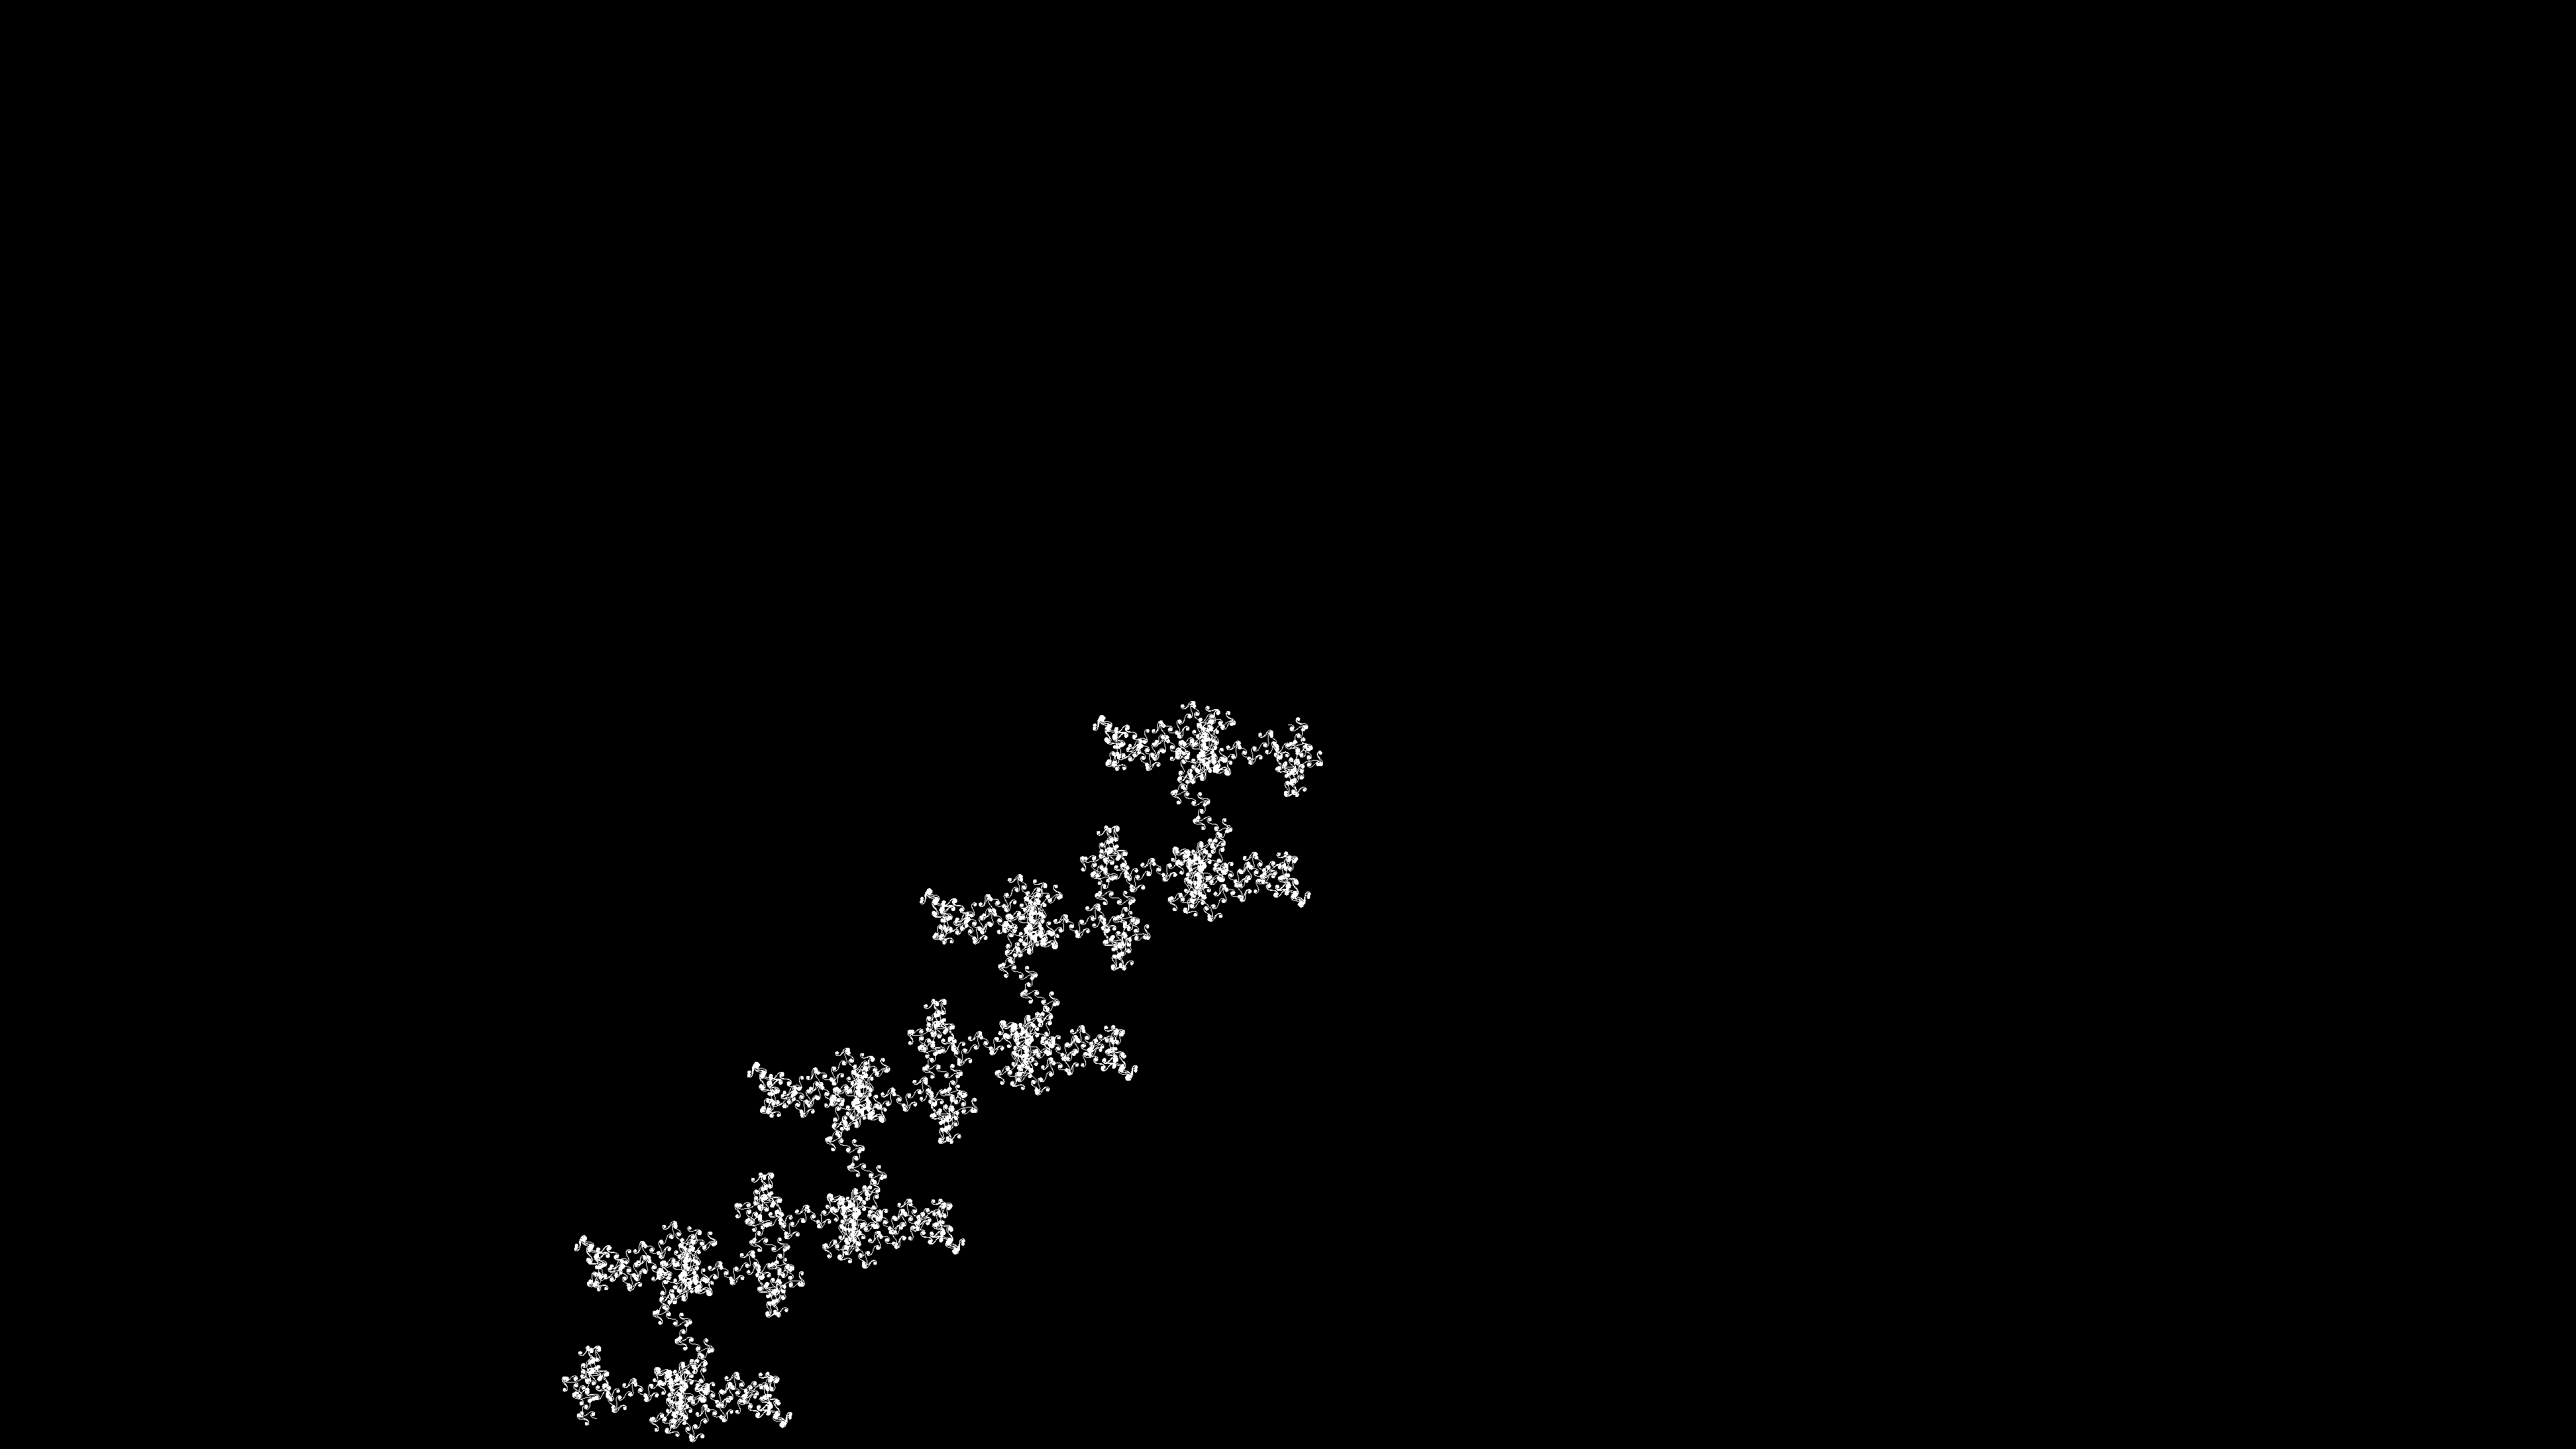
\includegraphics[width=\linewidth]{./stepsplusoneimages/0000000112.png}
    \caption{tf p=499 q=200209 theta=000 89726236.png}
  \end{subfigure}
  \caption{n=110 s=400 s+1=401}
  \label{fig:n=110}
\end{figure}
\begin{figure}[H]
  \centering
  \begin{subfigure}[t]{0.48\textwidth}
    \centering
    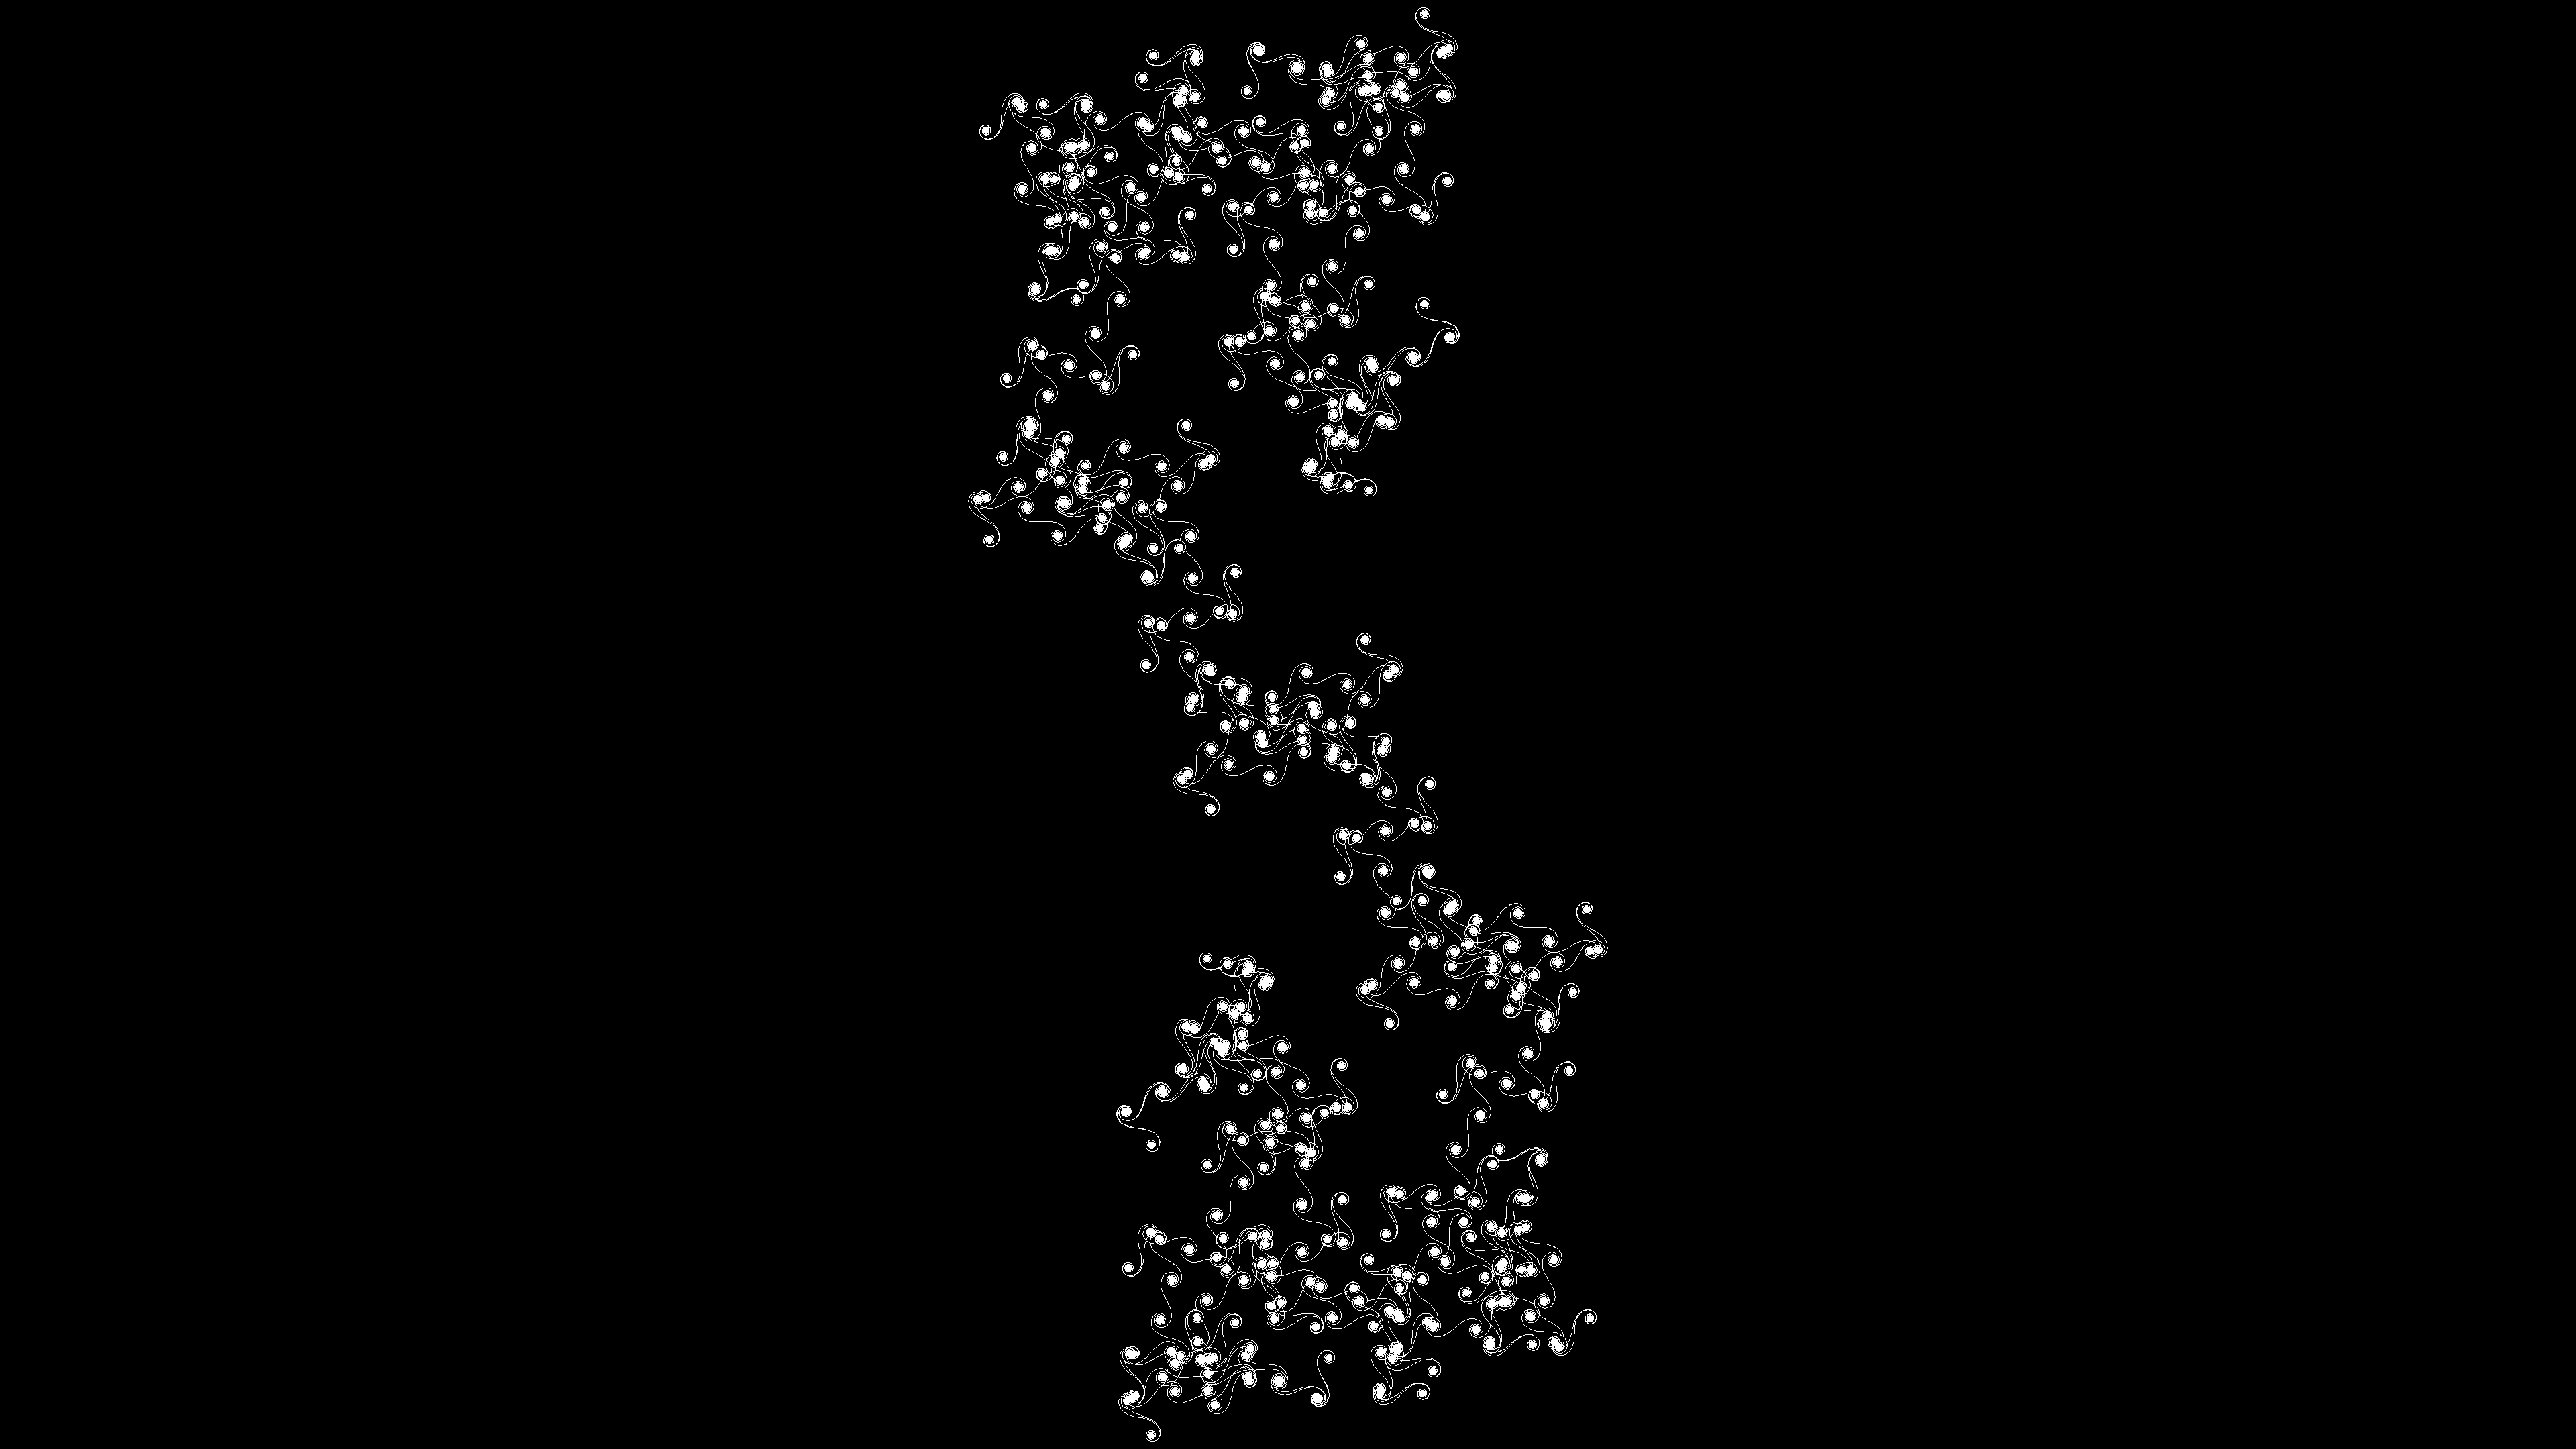
\includegraphics[width=\linewidth]{./stepsplusoneimages/0000000113.png}
    \caption{tf p=499 q=199712 theta=000 89949527.png}
  \end{subfigure}
  \begin{subfigure}[t]{0.48\textwidth}
    \centering
    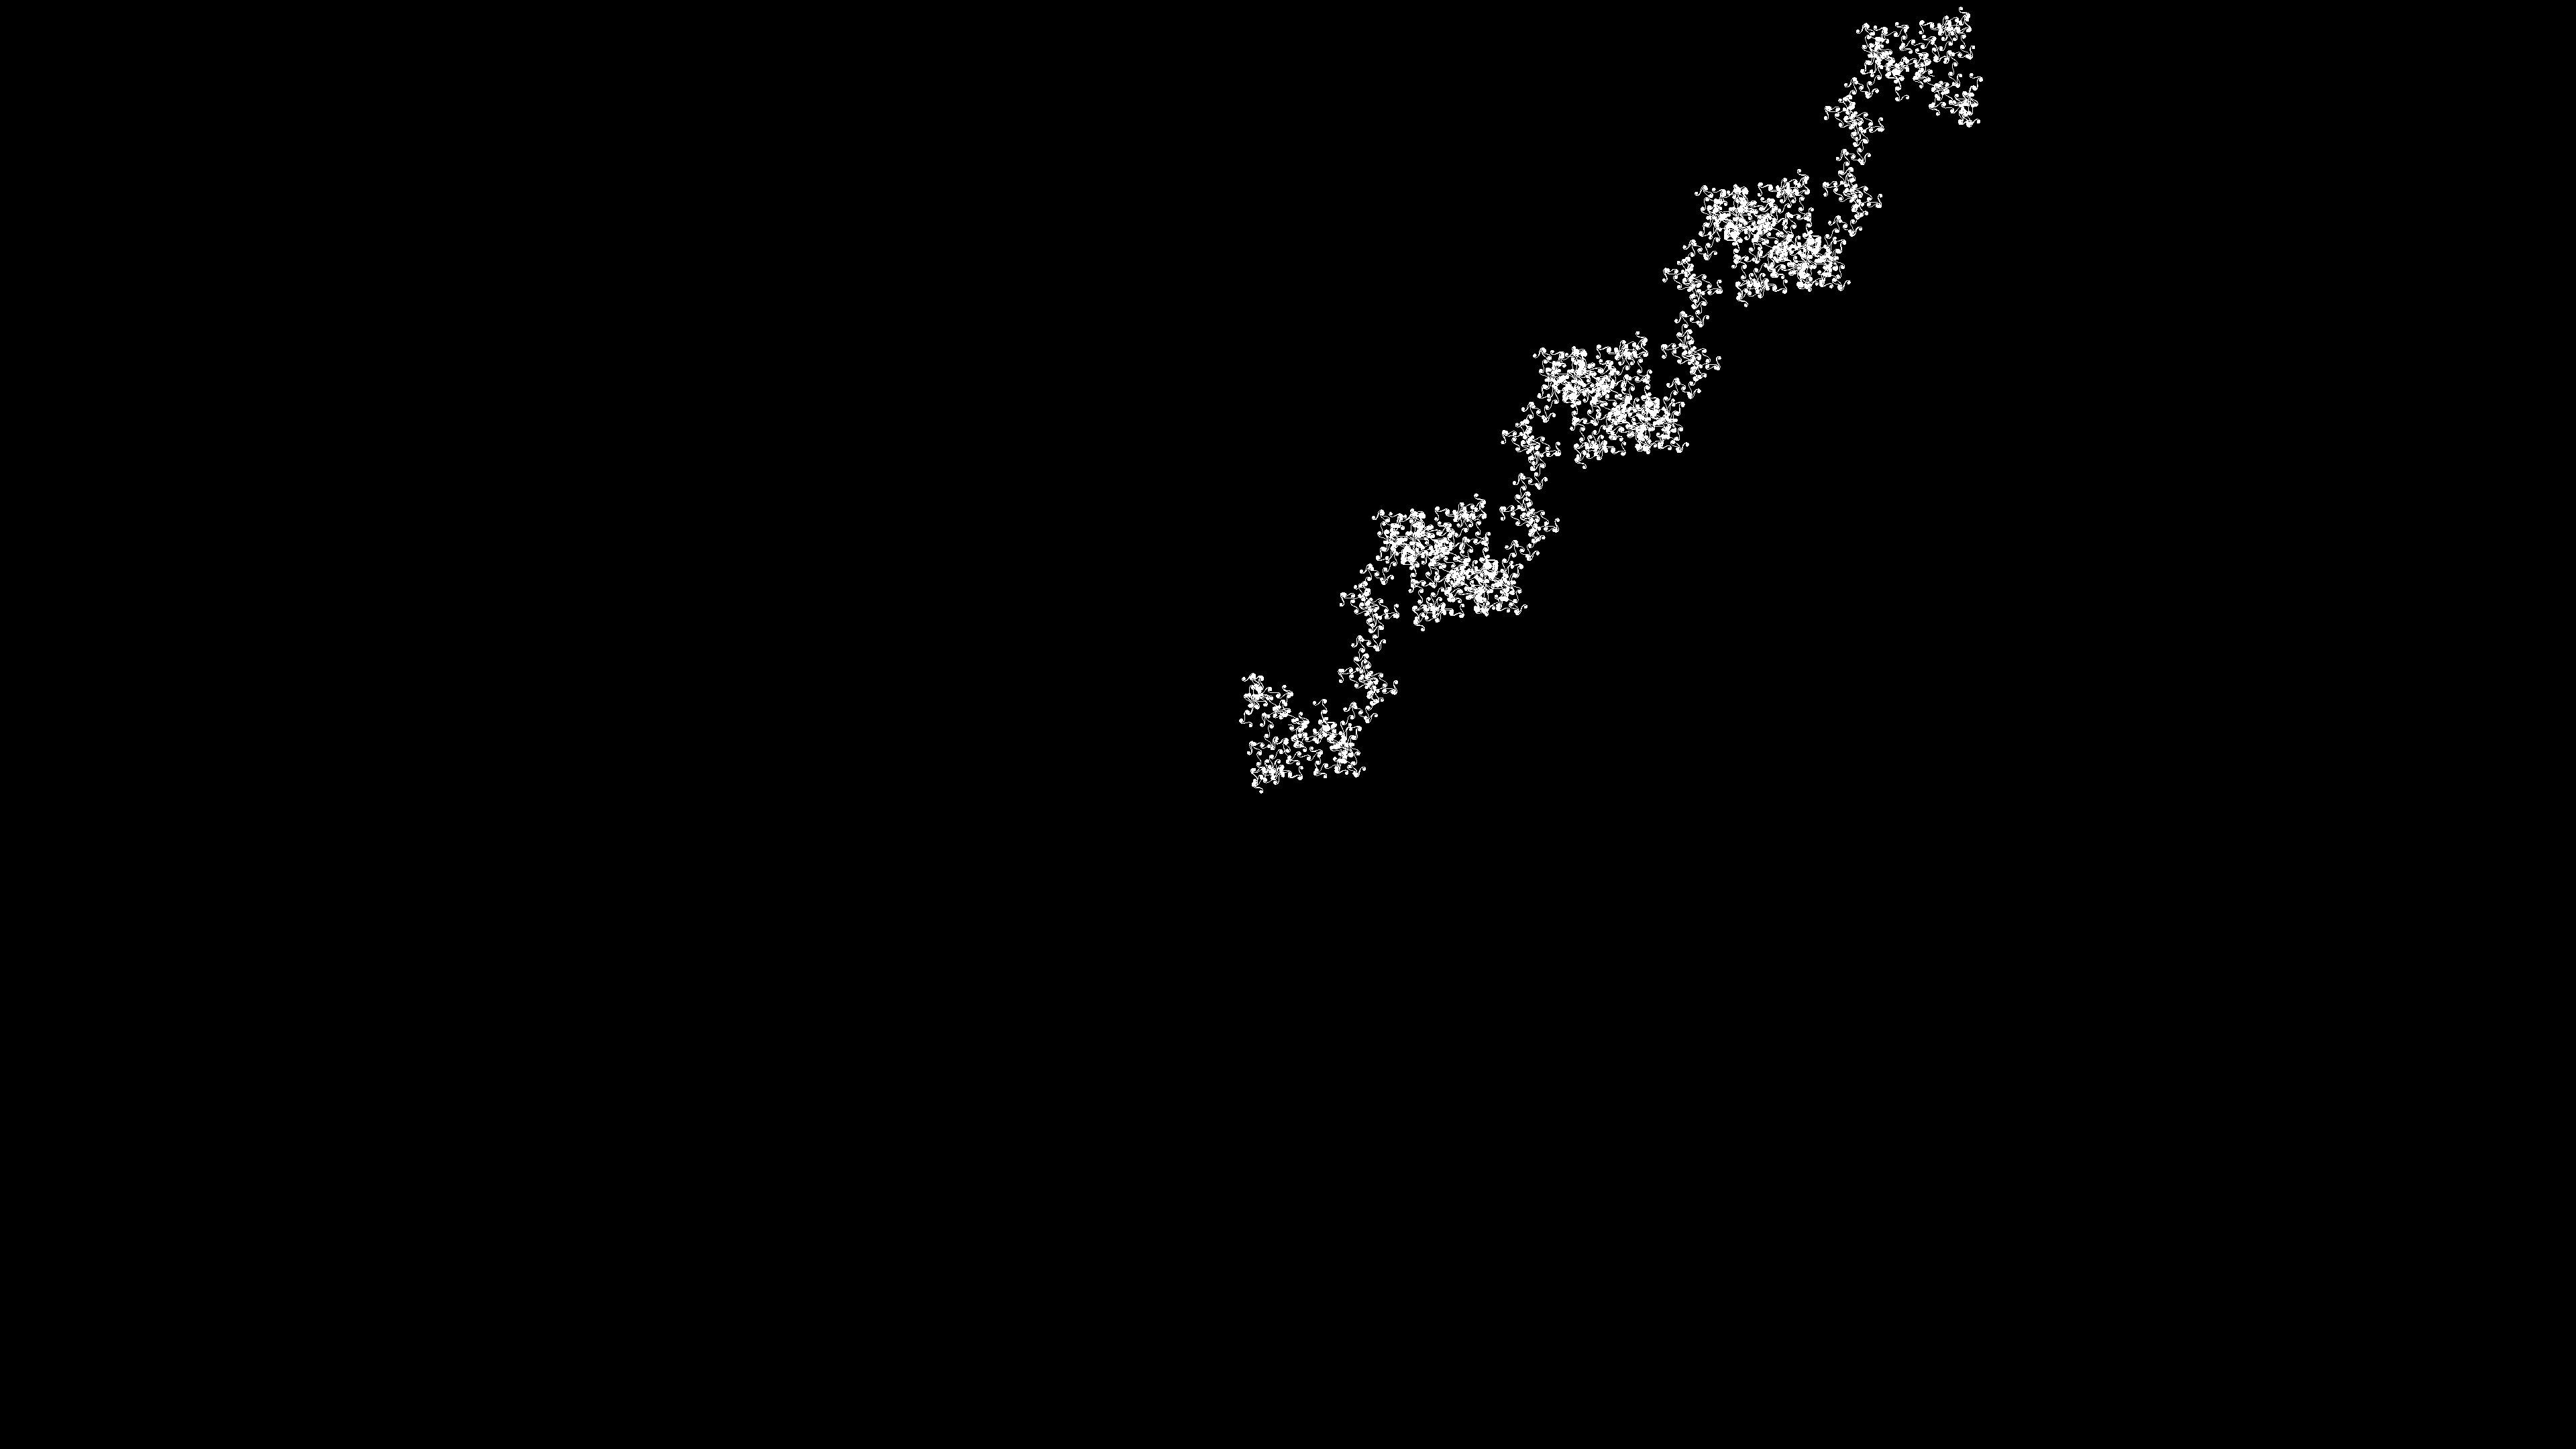
\includegraphics[width=\linewidth]{./stepsplusoneimages/0000000114.png}
    \caption{tf p=499 q=200211 theta=000 89725340.png}
  \end{subfigure}
  \caption{n=112 s=400 s+1=401}
  \label{fig:n=112}
\end{figure}
\begin{figure}[H]
  \centering
  \begin{subfigure}[t]{0.48\textwidth}
    \centering
    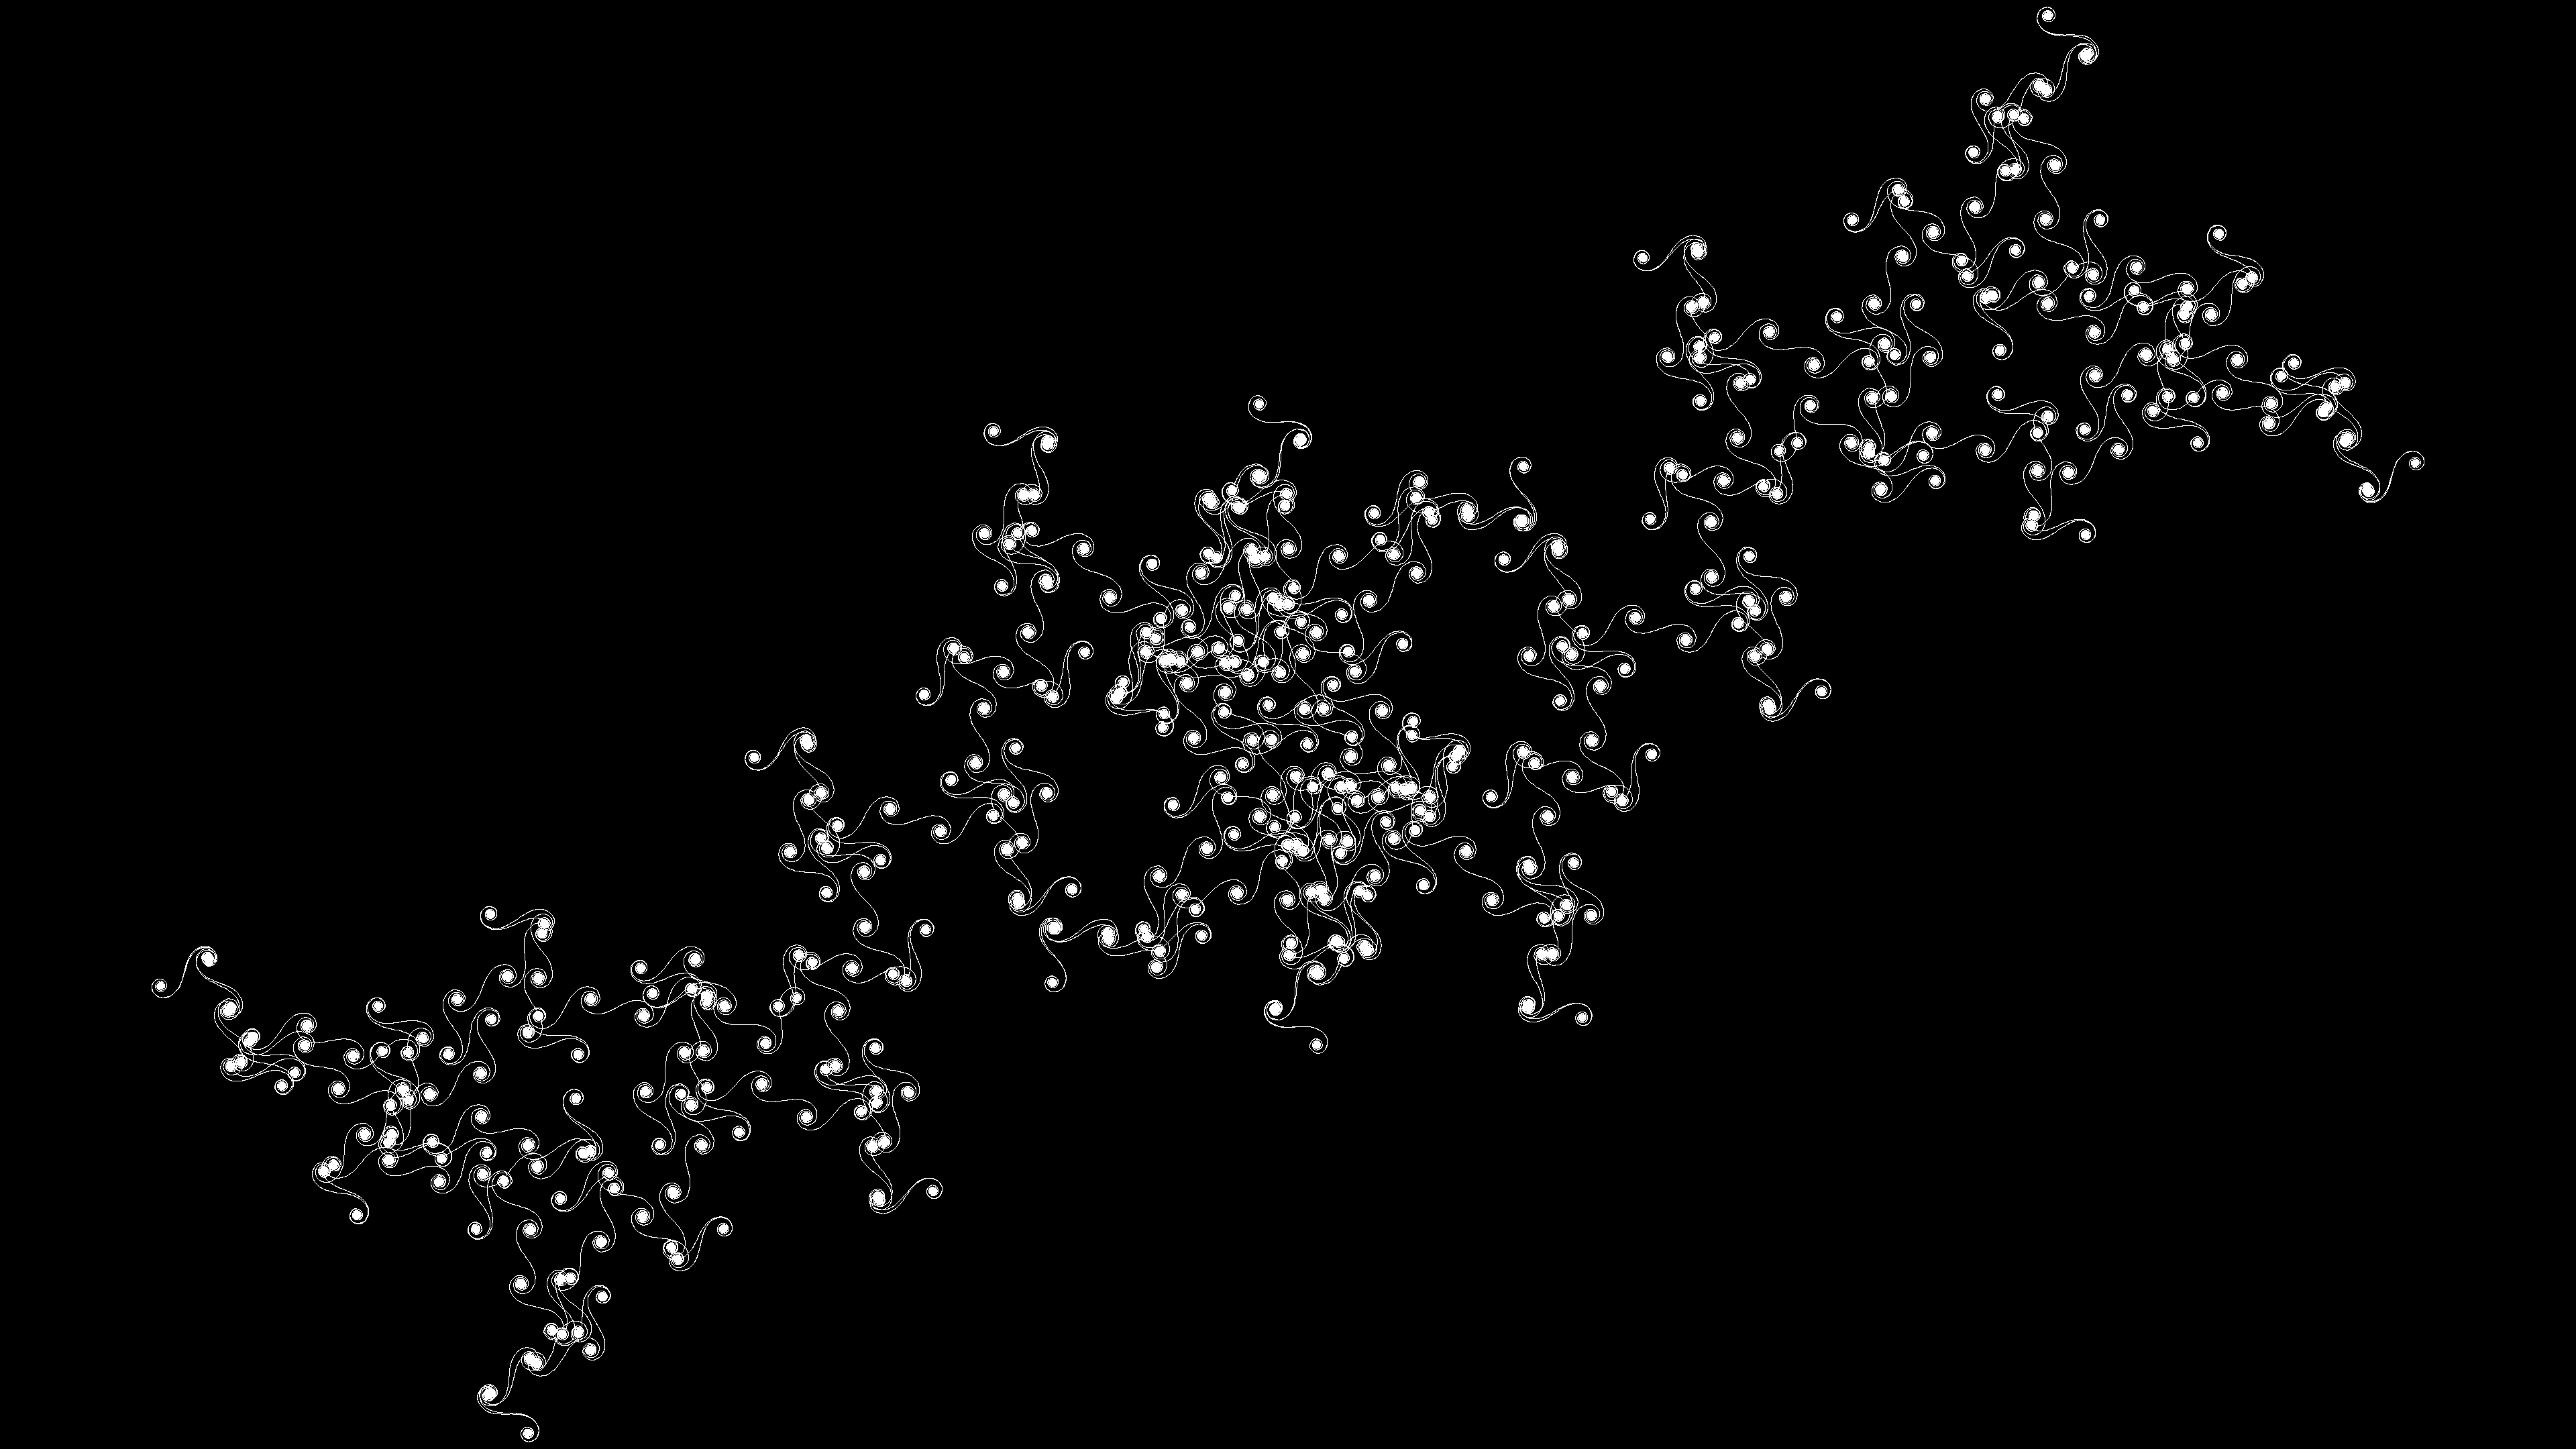
\includegraphics[width=\linewidth]{./stepsplusoneimages/0000000115.png}
    \caption{tf p=499 q=199714 theta=000 89948627.png}
  \end{subfigure}
  \begin{subfigure}[t]{0.48\textwidth}
    \centering
    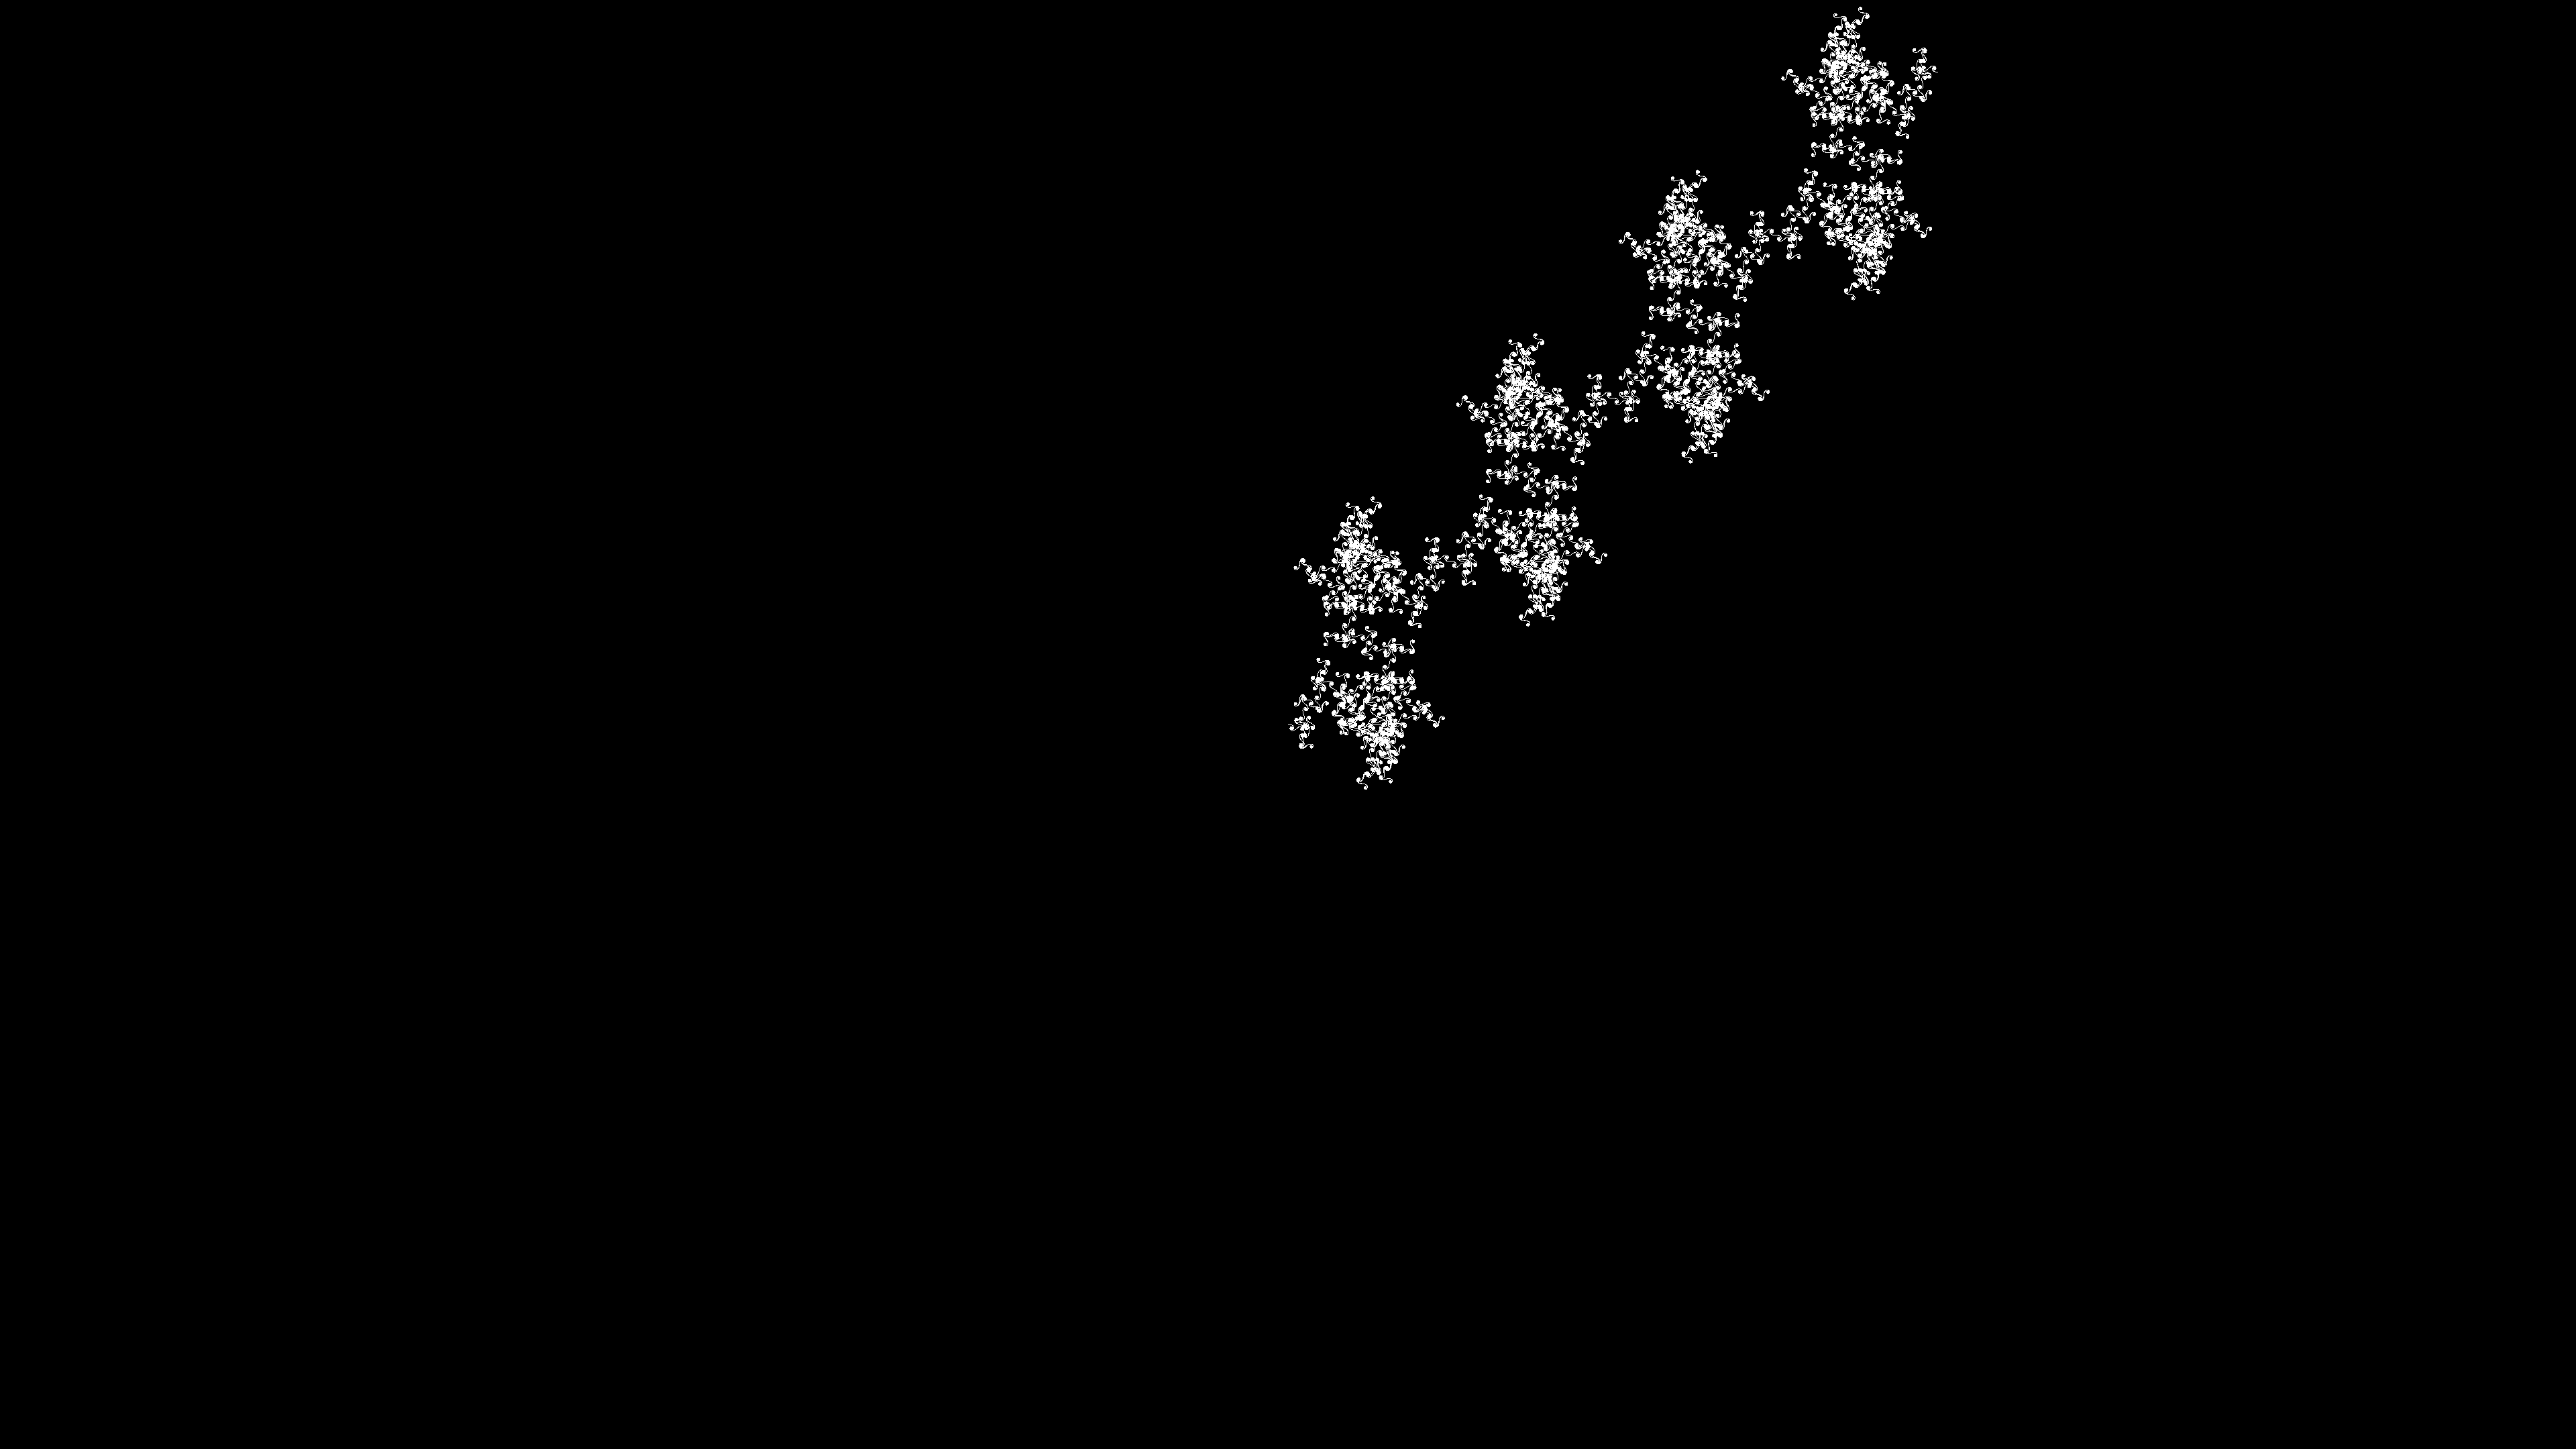
\includegraphics[width=\linewidth]{./stepsplusoneimages/0000000116.png}
    \caption{tf p=499 q=200213 theta=000 89724443.png}
  \end{subfigure}
  \caption{n=114 s=400 s+1=401}
  \label{fig:n=114}
\end{figure}
\begin{figure}[H]
  \centering
  \begin{subfigure}[t]{0.48\textwidth}
    \centering
    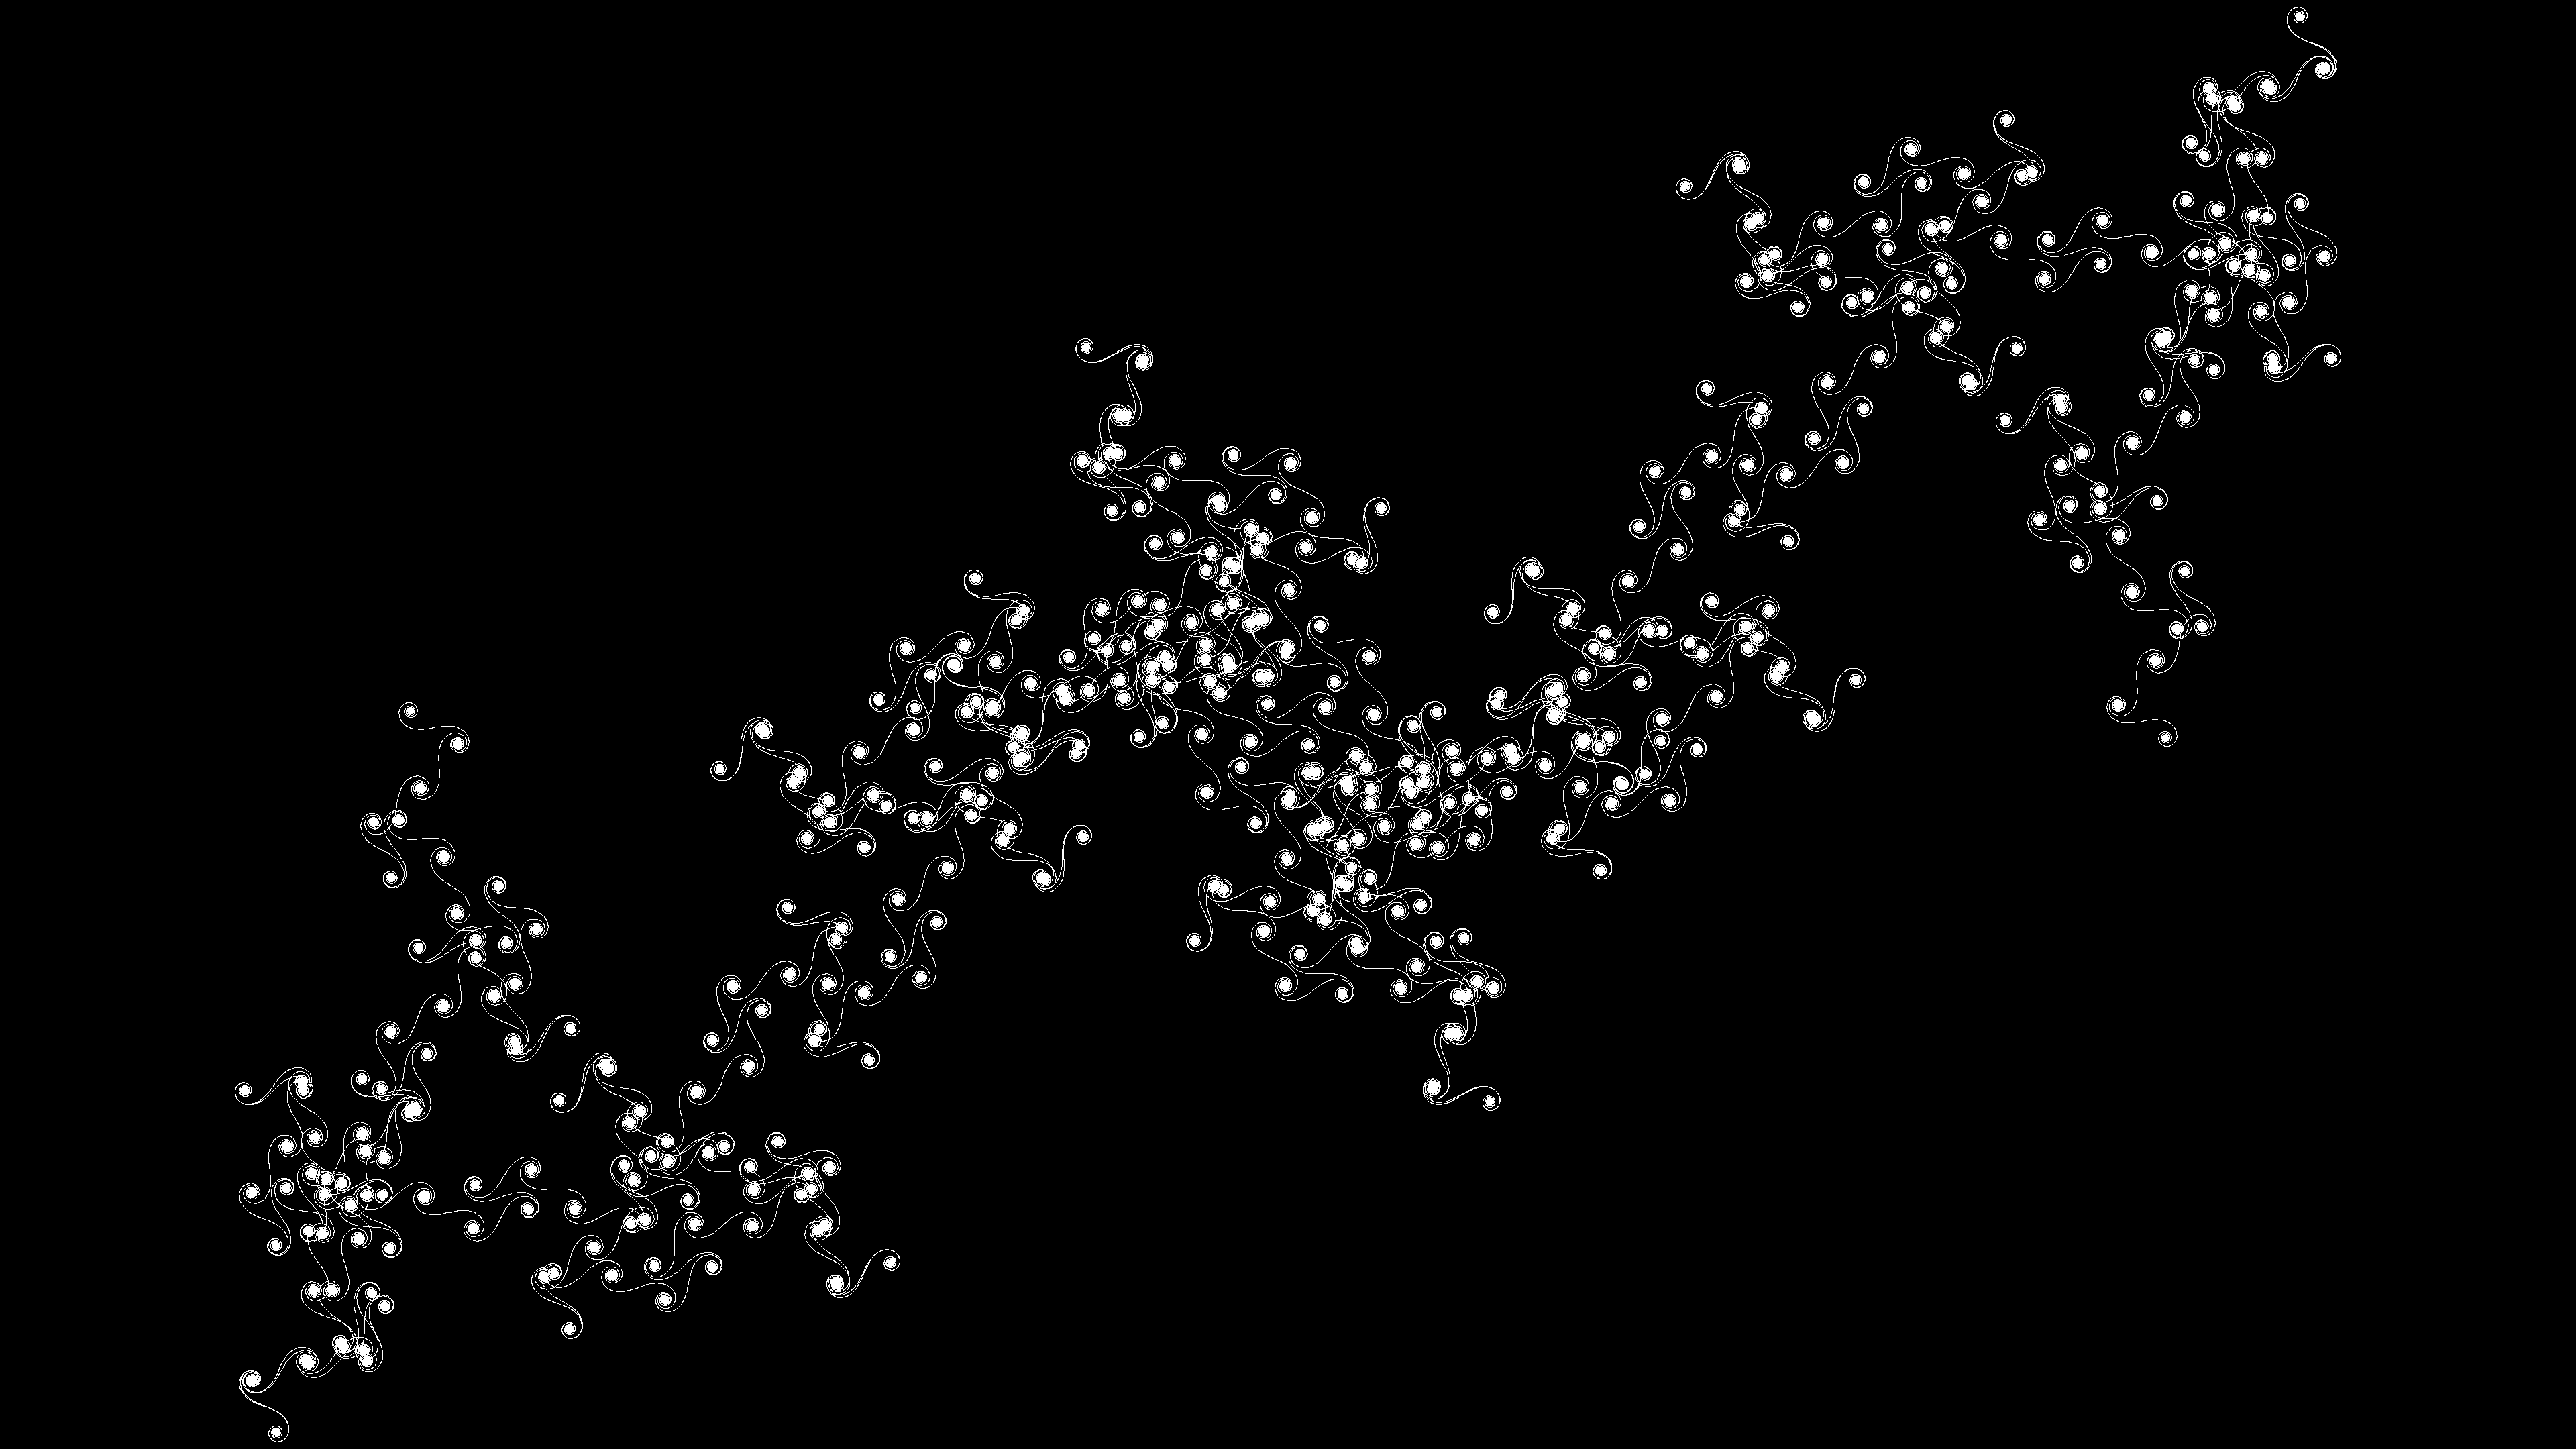
\includegraphics[width=\linewidth]{./stepsplusoneimages/0000000117.png}
    \caption{tf p=499 q=199716 theta=000 89947726.png}
  \end{subfigure}
  \begin{subfigure}[t]{0.48\textwidth}
    \centering
    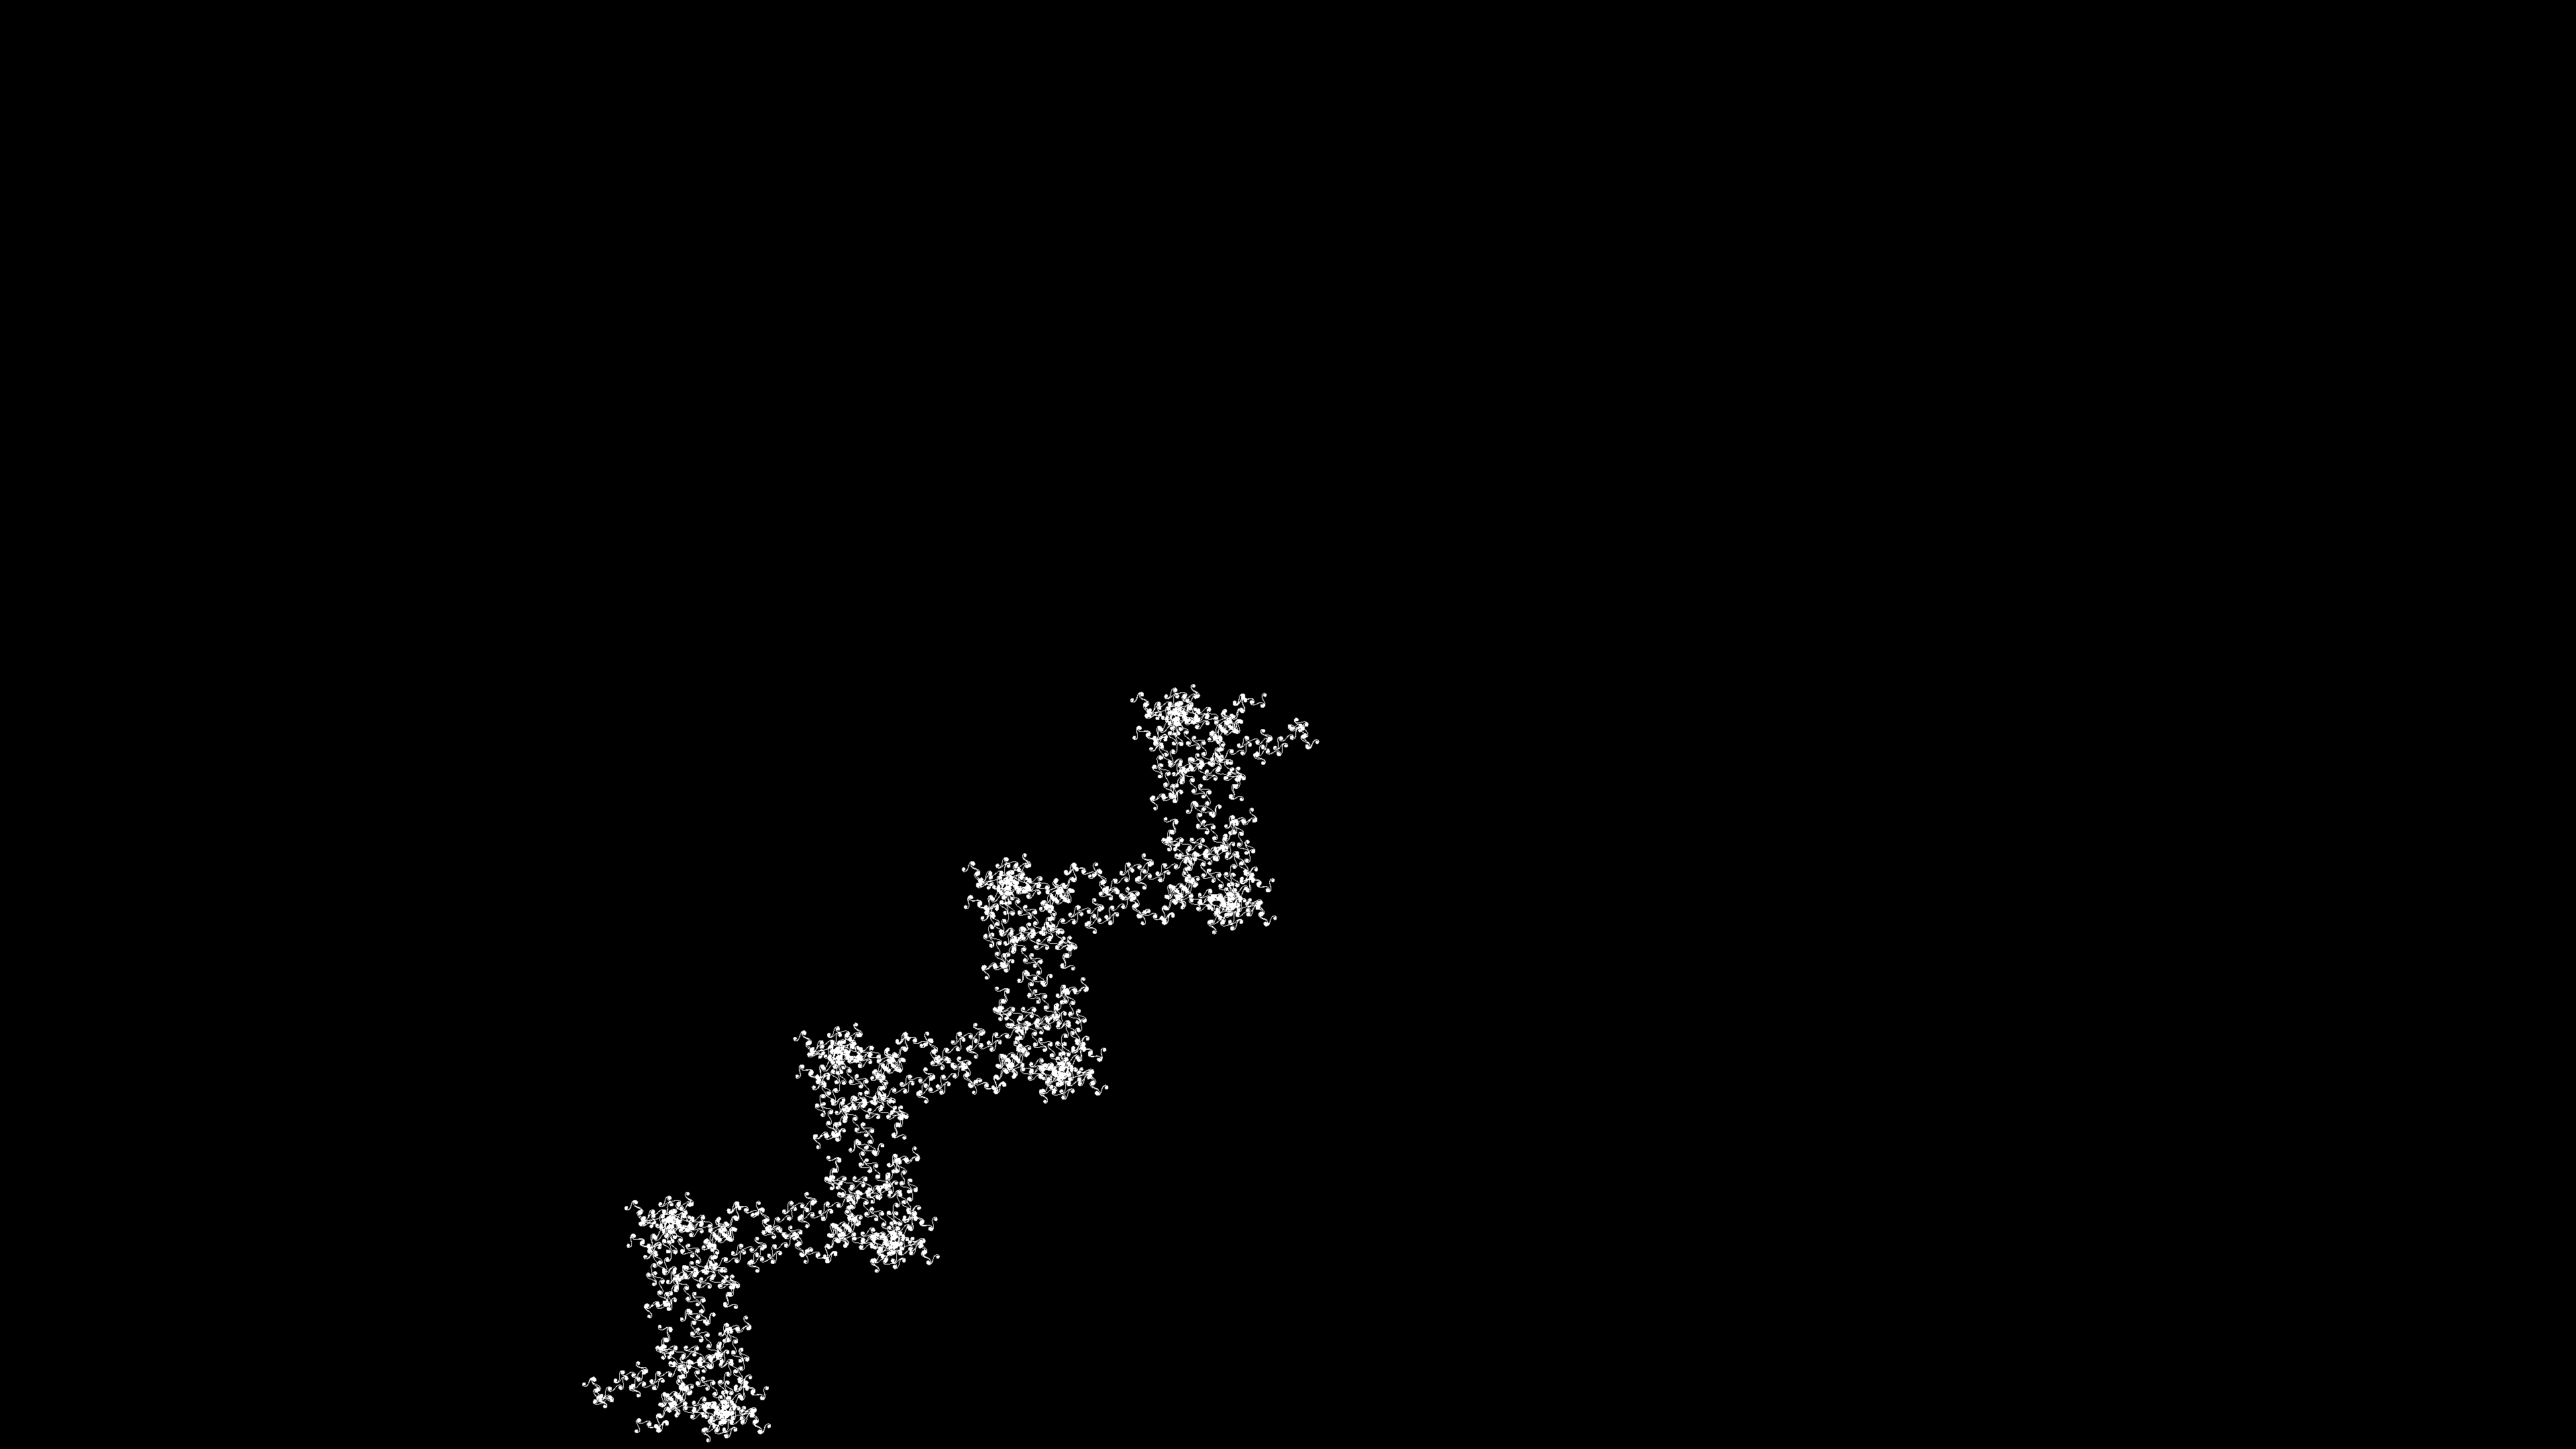
\includegraphics[width=\linewidth]{./stepsplusoneimages/0000000118.png}
    \caption{tf p=499 q=200215 theta=000 89723547.png}
  \end{subfigure}
  \caption{n=116 s=400 s+1=401}
  \label{fig:n=116}
\end{figure}
\begin{figure}[H]
  \centering
  \begin{subfigure}[t]{0.48\textwidth}
    \centering
    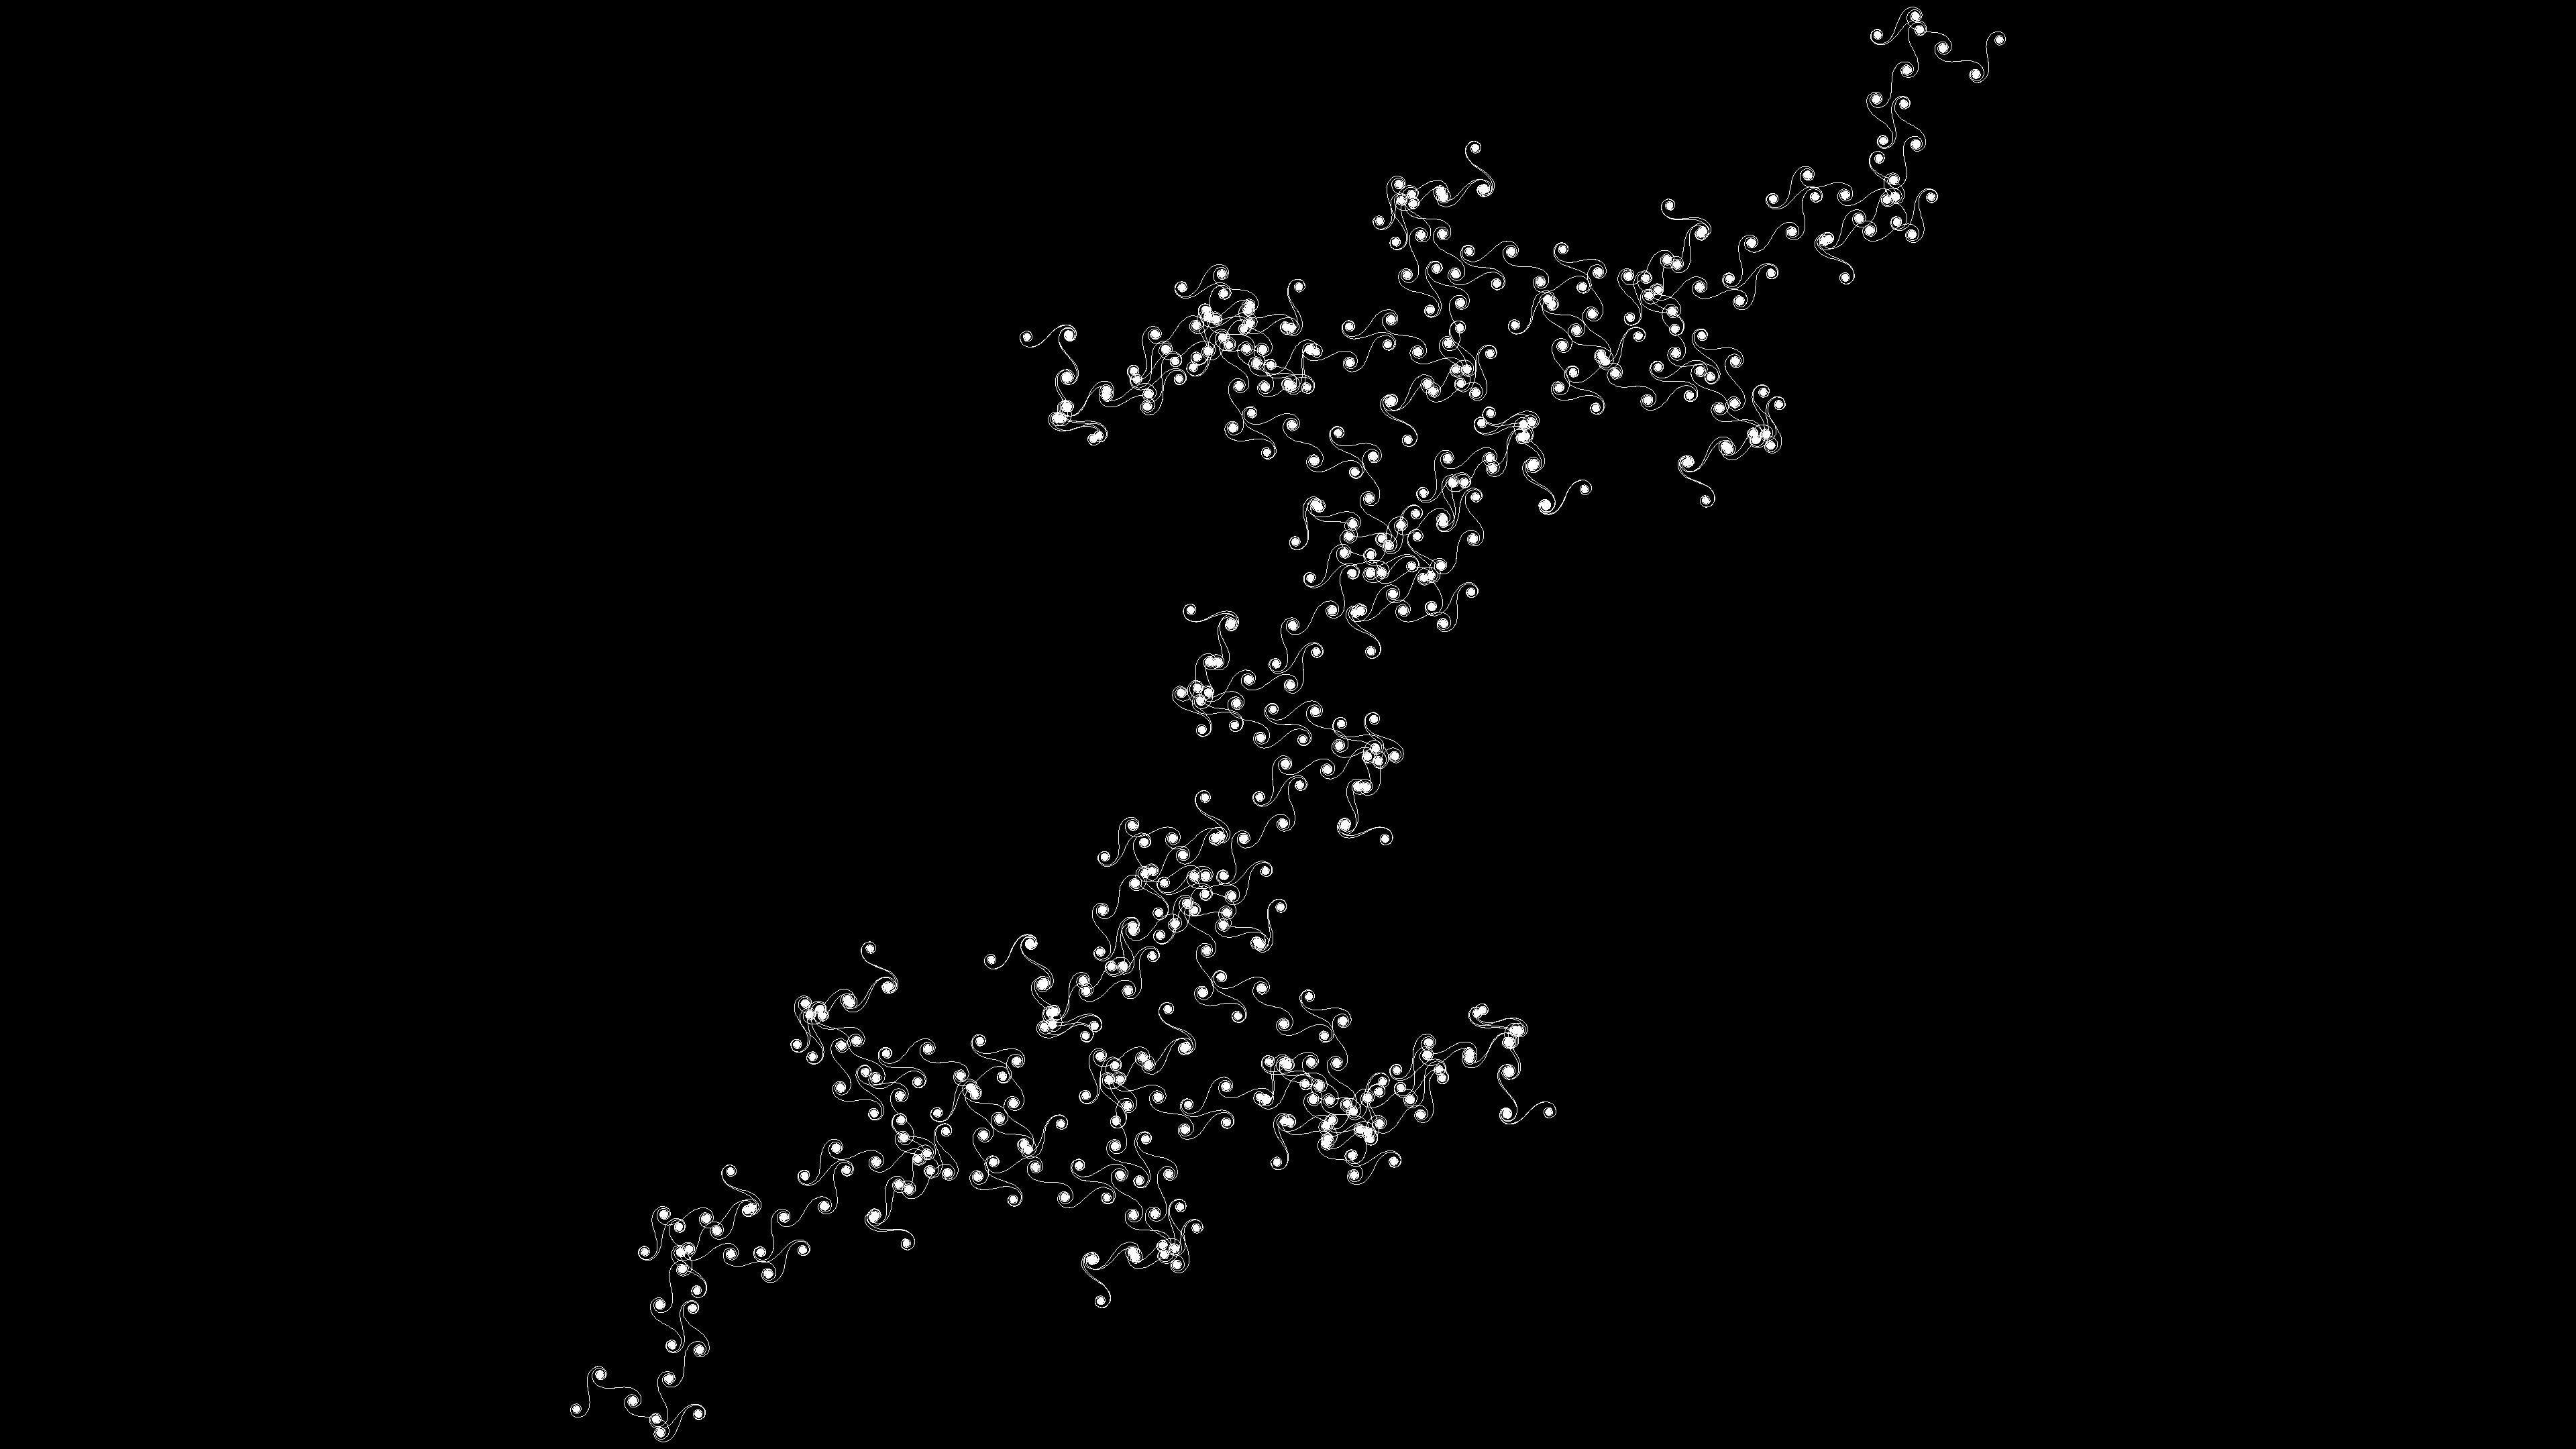
\includegraphics[width=\linewidth]{./stepsplusoneimages/0000000119.png}
    \caption{tf p=499 q=199718 theta=000 89946825.png}
  \end{subfigure}
  \begin{subfigure}[t]{0.48\textwidth}
    \centering
    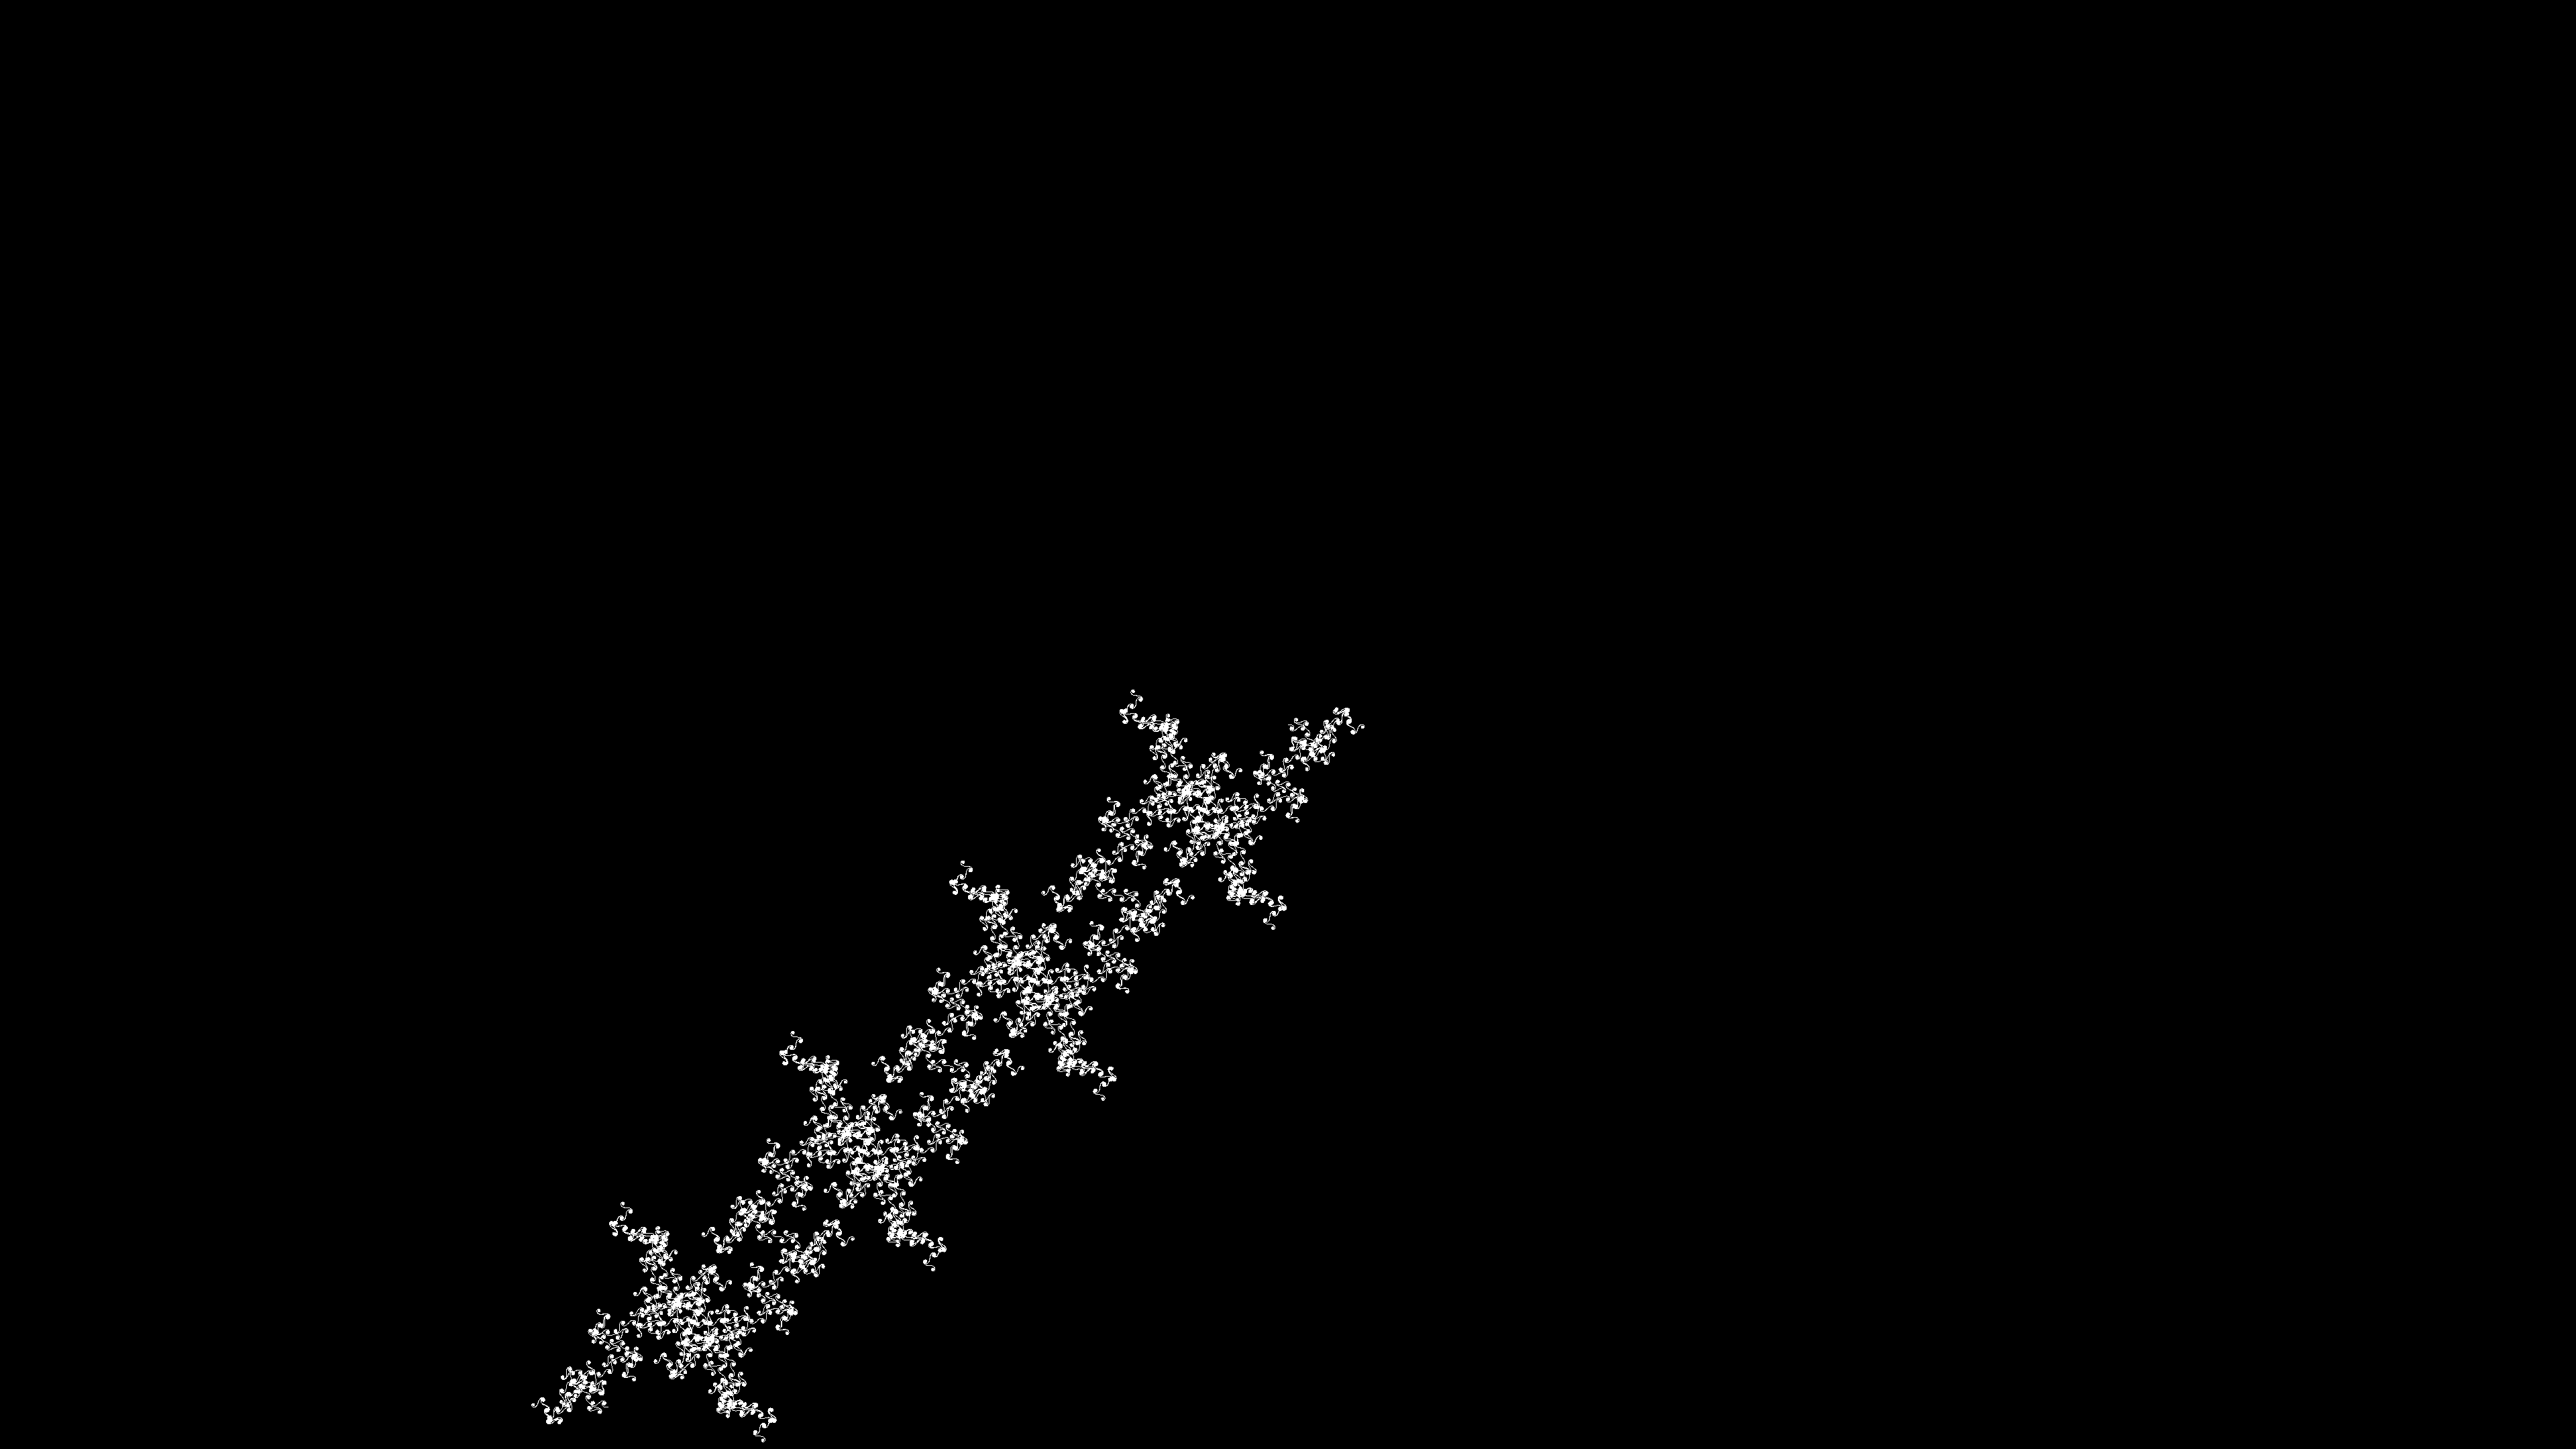
\includegraphics[width=\linewidth]{./stepsplusoneimages/0000000120.png}
    \caption{tf p=499 q=200217 theta=000 89722651.png}
  \end{subfigure}
  \caption{n=118 s=400 s+1=401}
  \label{fig:n=118}
\end{figure}
\begin{figure}[H]
  \centering
  \begin{subfigure}[t]{0.48\textwidth}
    \centering
    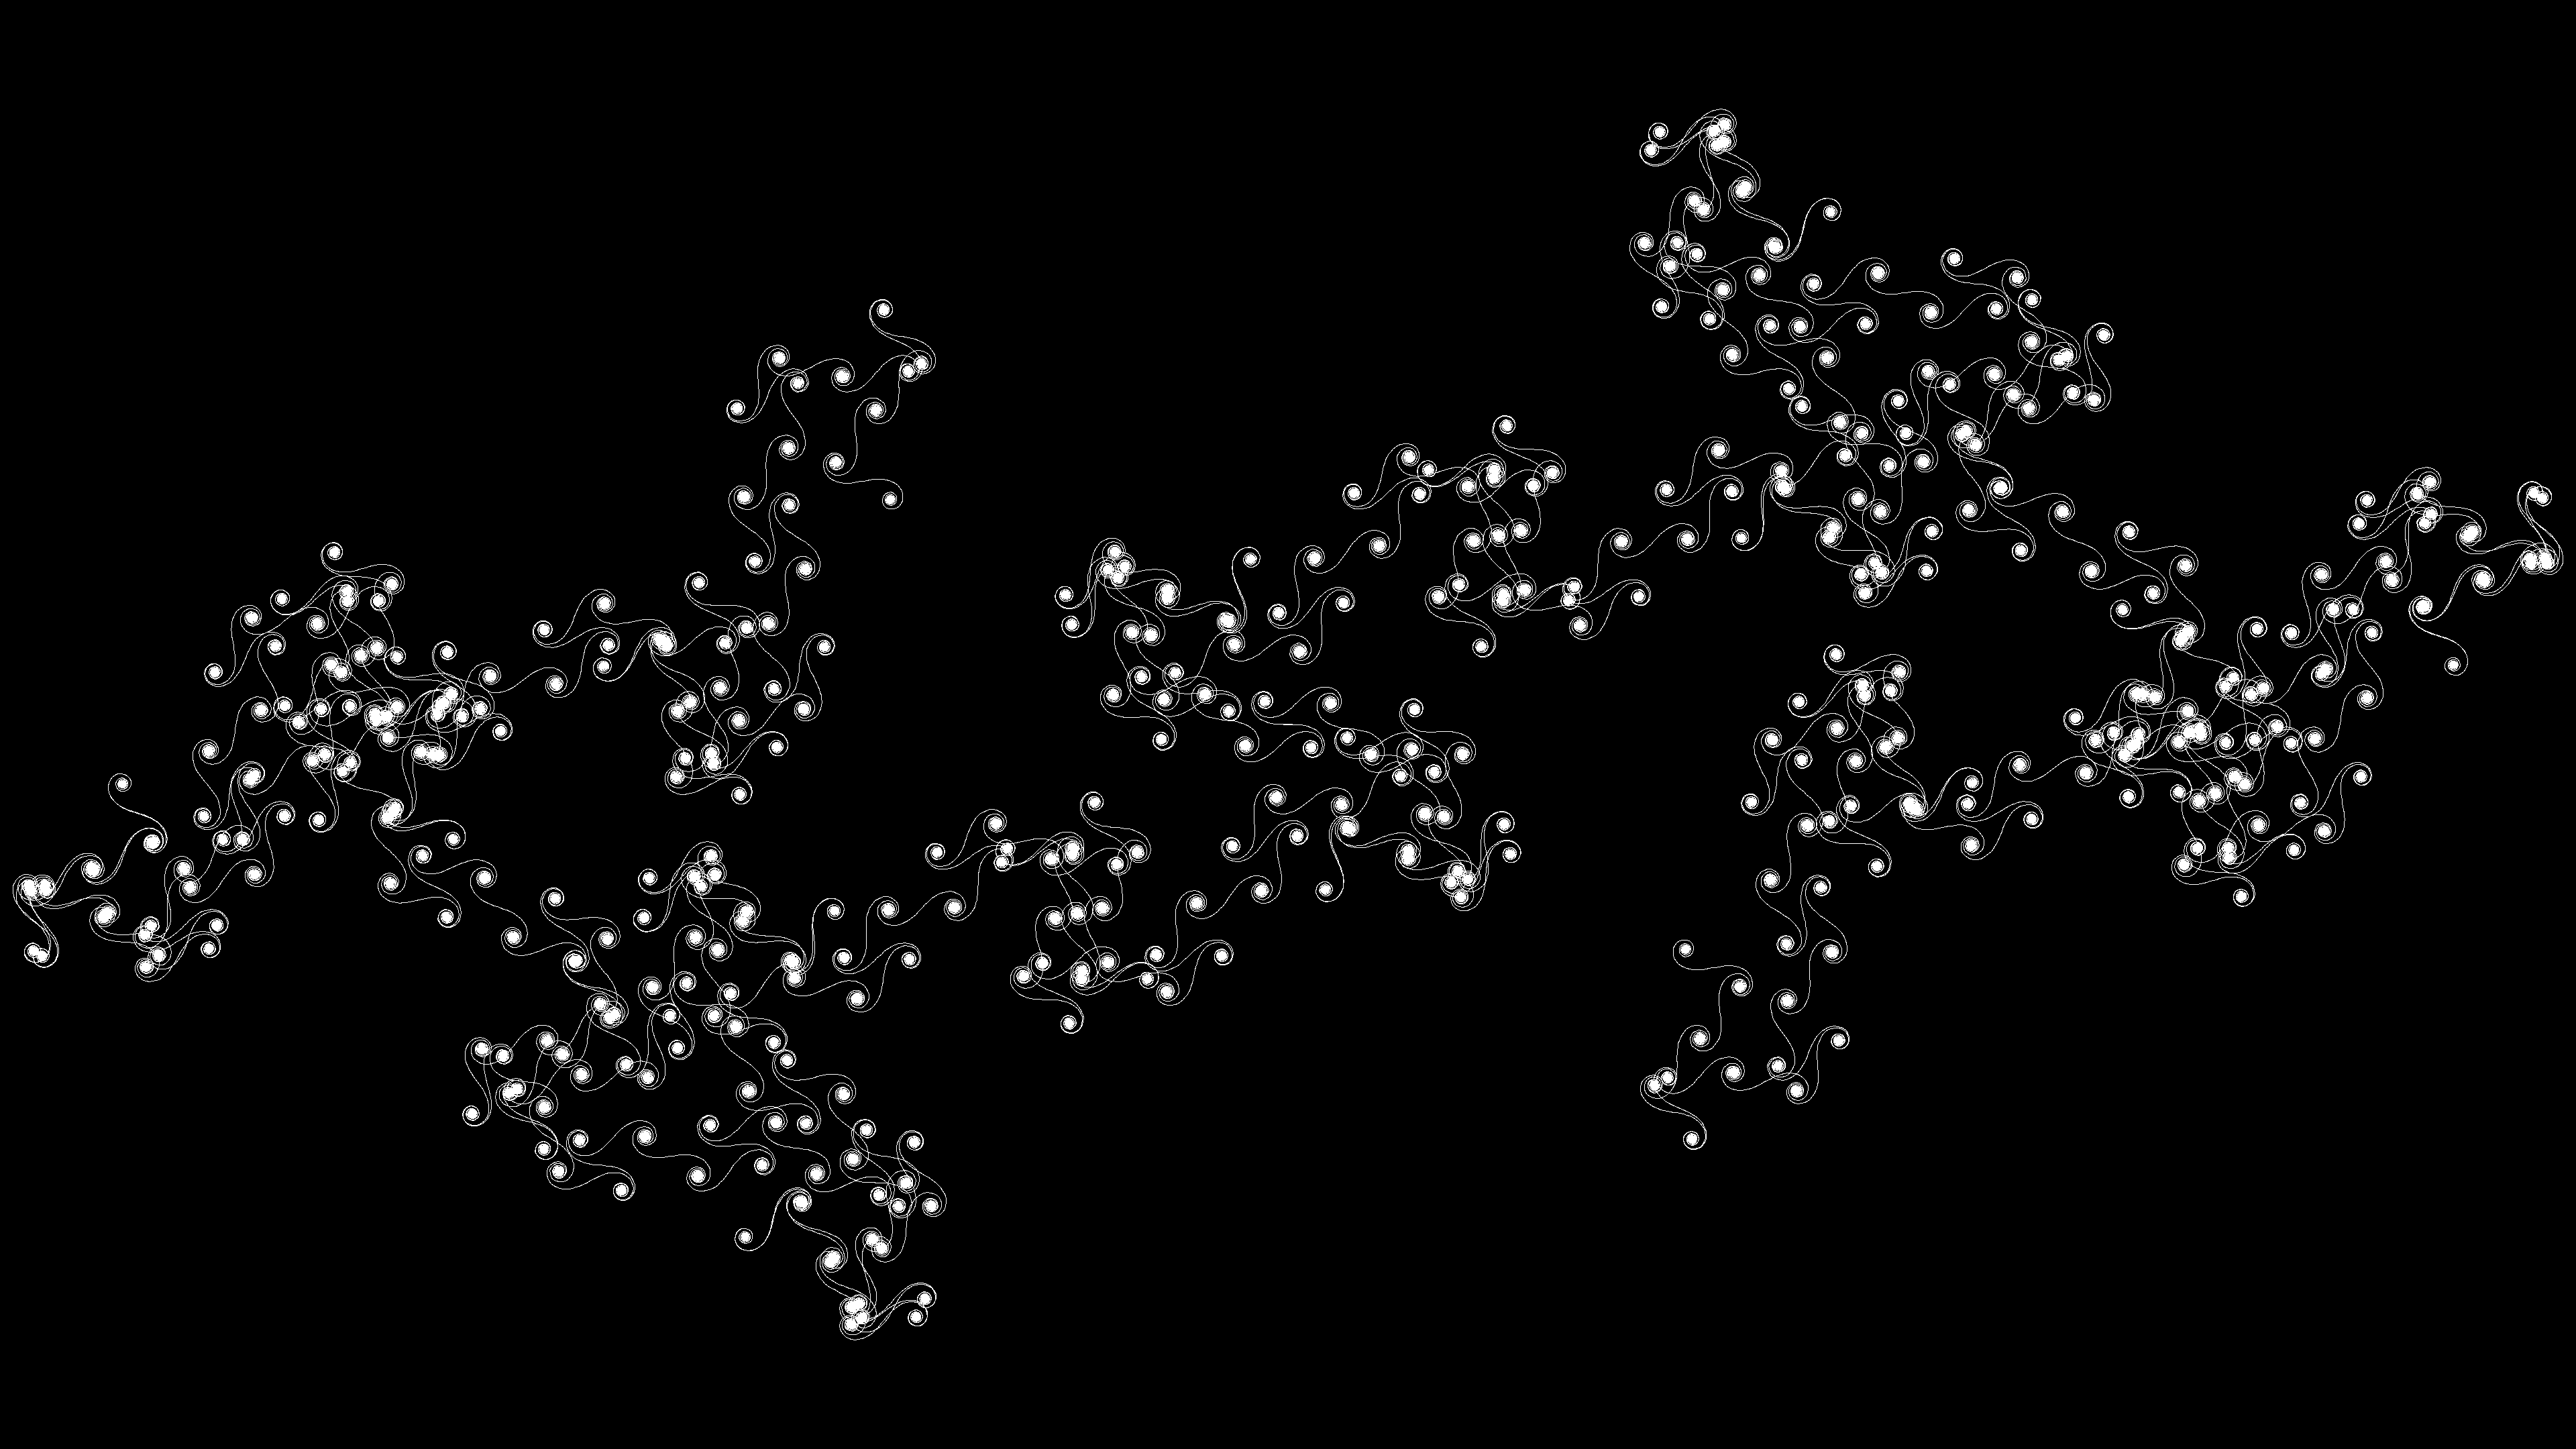
\includegraphics[width=\linewidth]{./stepsplusoneimages/0000000121.png}
    \caption{tf p=499 q=199720 theta=000 89945924.png}
  \end{subfigure}
  \begin{subfigure}[t]{0.48\textwidth}
    \centering
    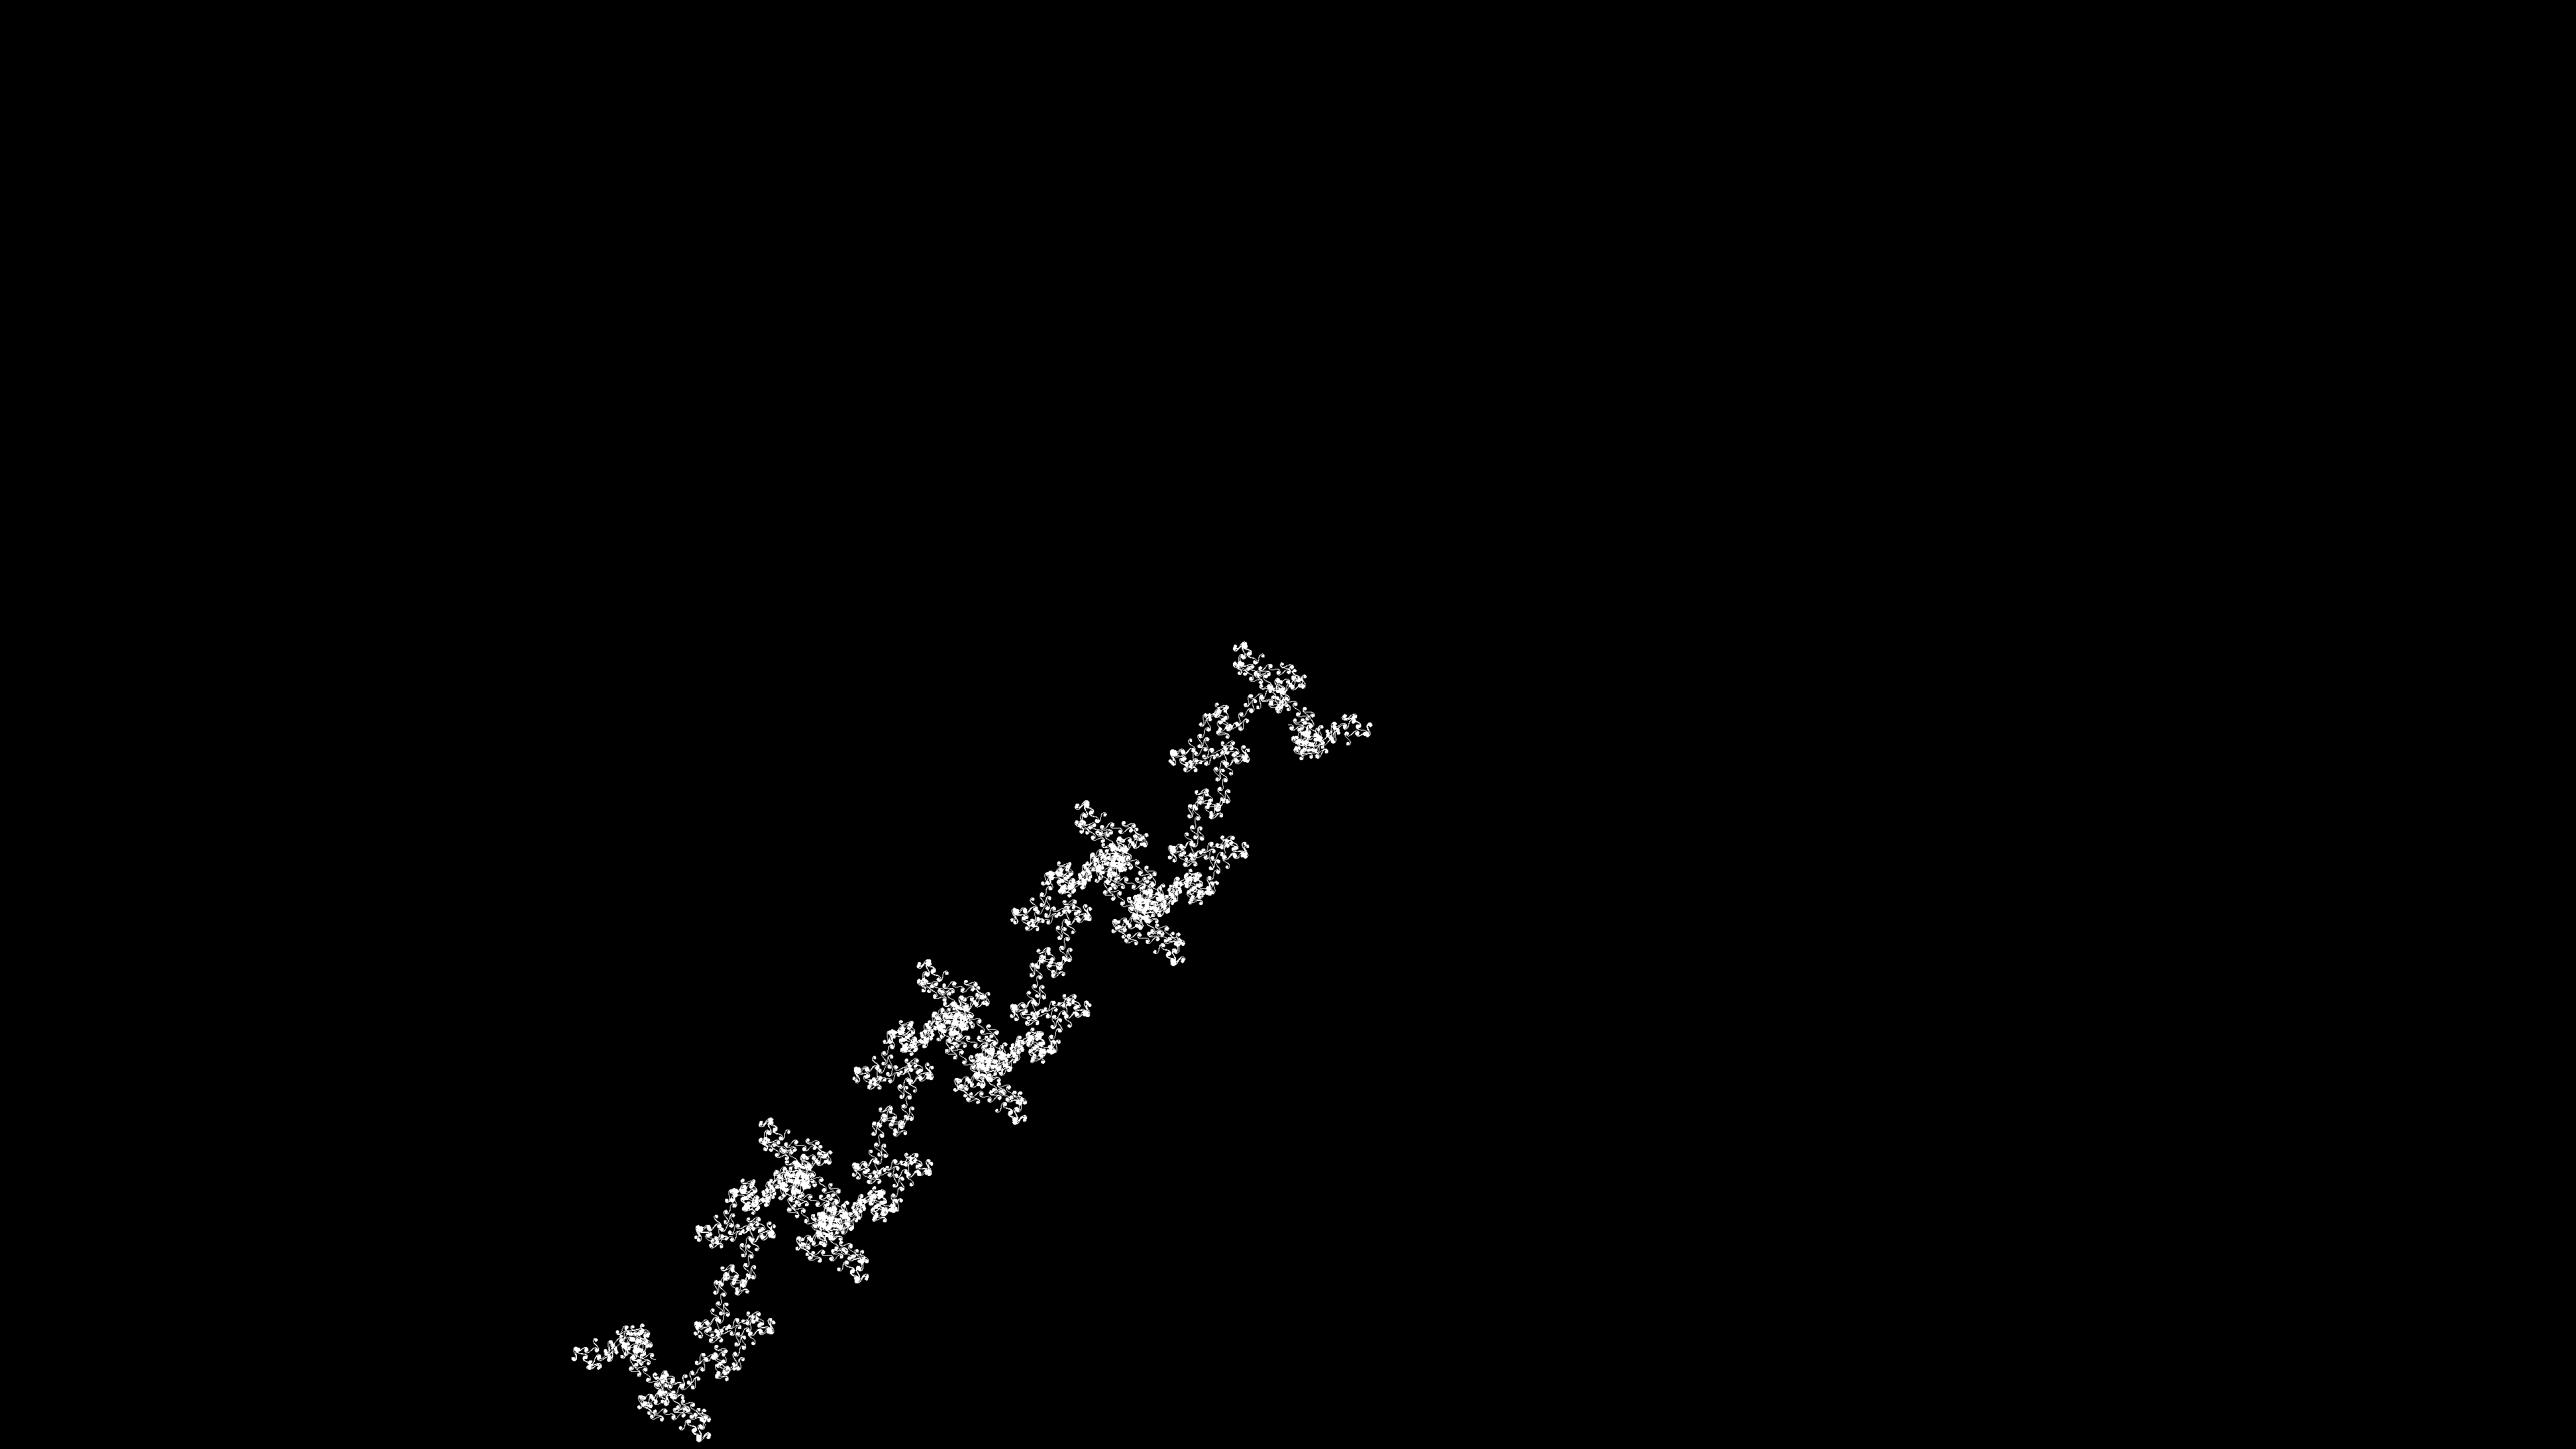
\includegraphics[width=\linewidth]{./stepsplusoneimages/0000000122.png}
    \caption{tf p=499 q=200219 theta=000 89721755.png}
  \end{subfigure}
  \caption{n=120 s=400 s+1=401}
  \label{fig:n=120}
\end{figure}
\begin{figure}[H]
  \centering
  \begin{subfigure}[t]{0.48\textwidth}
    \centering
    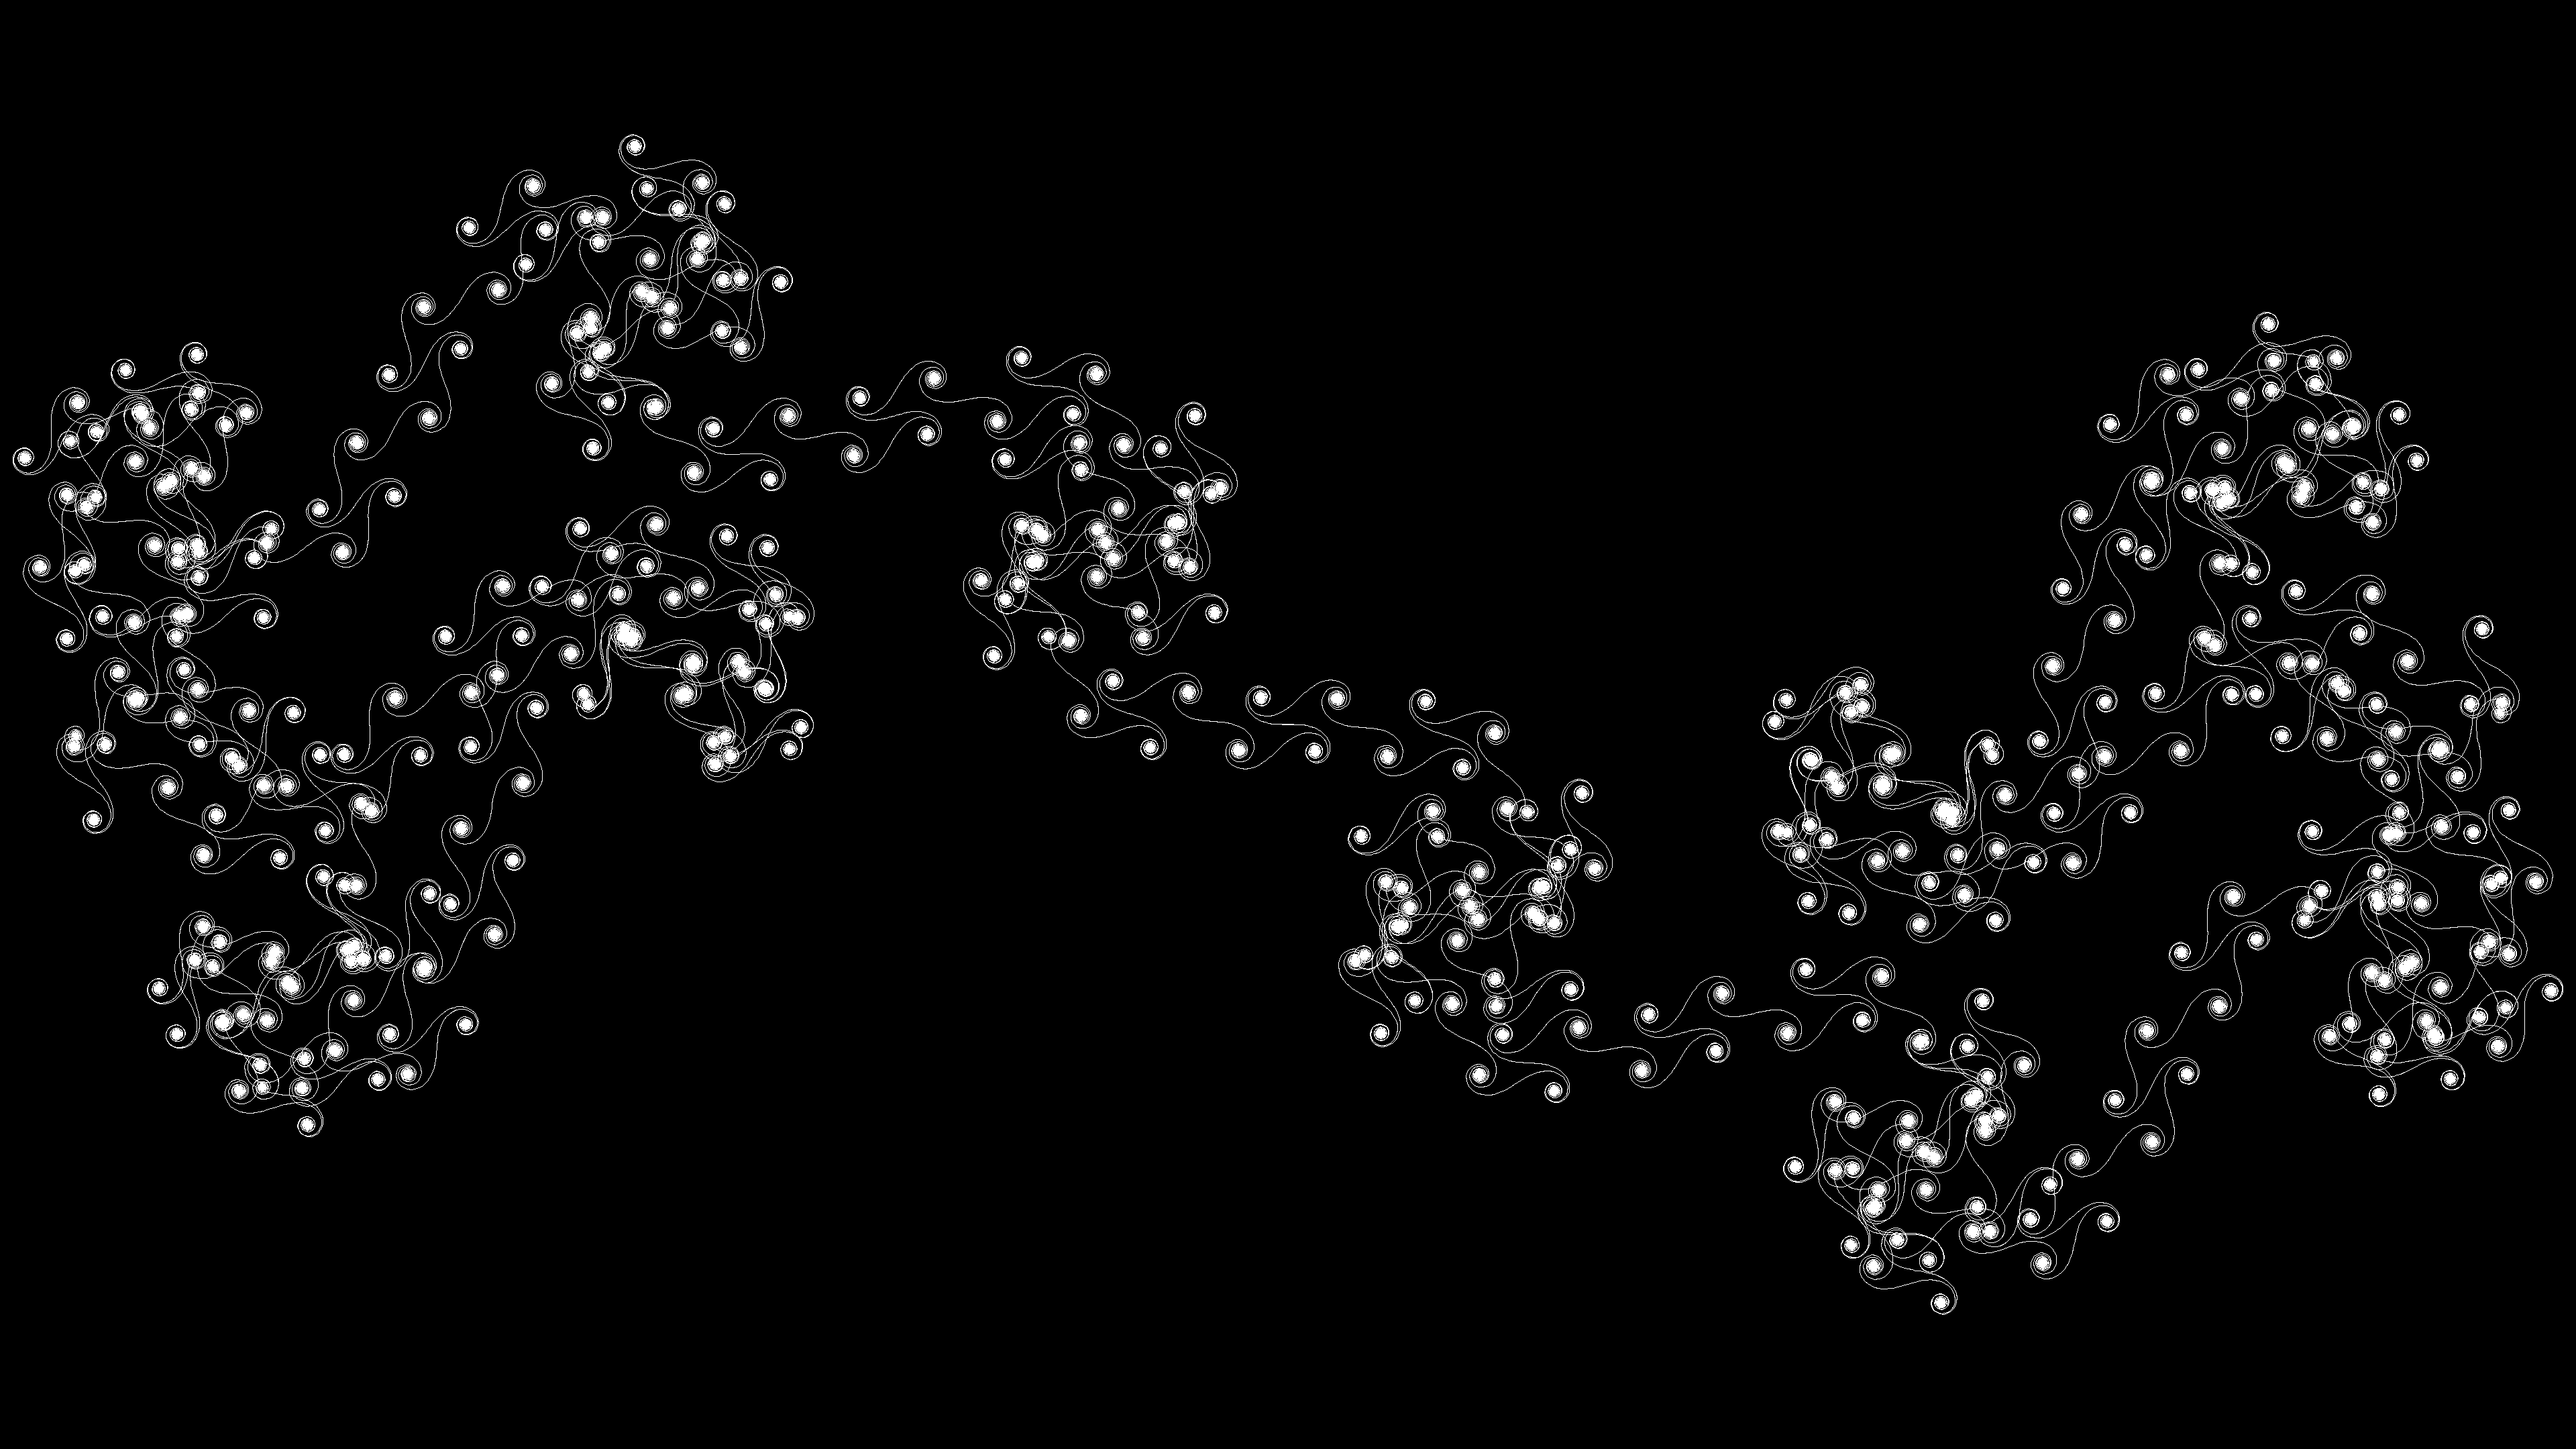
\includegraphics[width=\linewidth]{./stepsplusoneimages/0000000123.png}
    \caption{tf p=499 q=199722 theta=000 89945024.png}
  \end{subfigure}
  \begin{subfigure}[t]{0.48\textwidth}
    \centering
    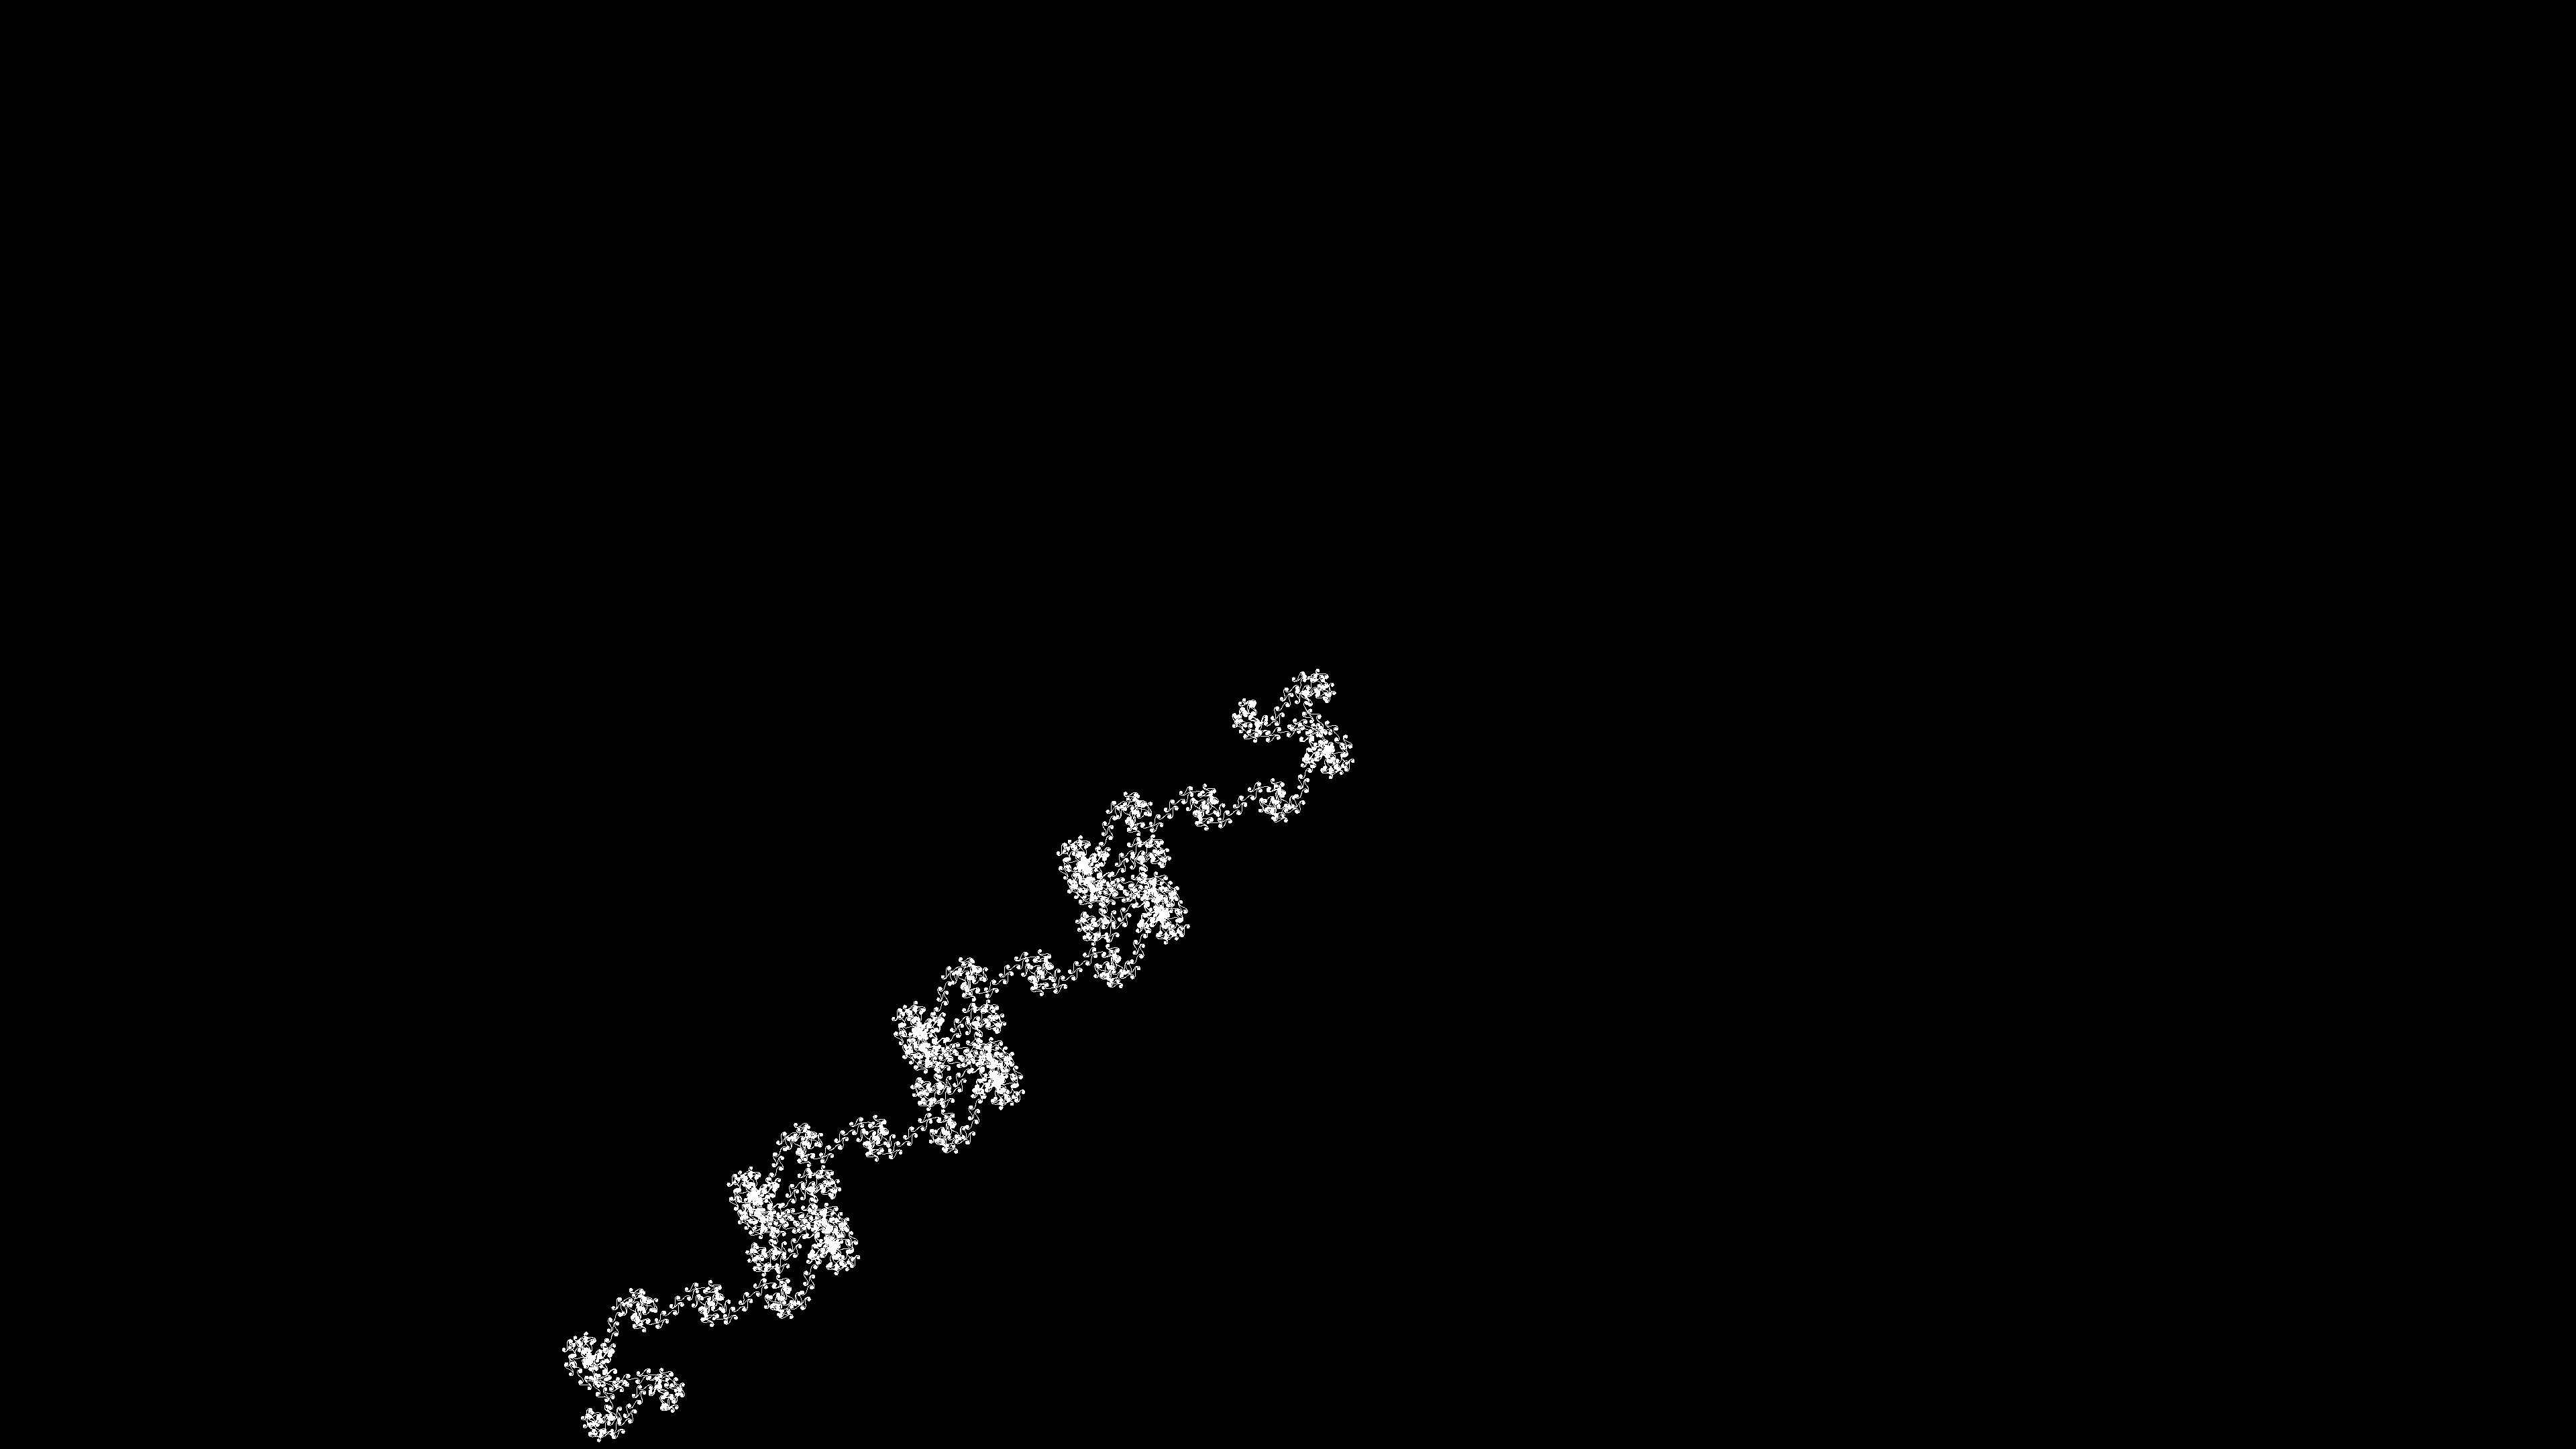
\includegraphics[width=\linewidth]{./stepsplusoneimages/0000000124.png}
    \caption{tf p=499 q=200221 theta=000 89720858.png}
  \end{subfigure}
  \caption{n=122 s=400 s+1=401}
  \label{fig:n=122}
\end{figure}
\begin{figure}[H]
  \centering
  \begin{subfigure}[t]{0.48\textwidth}
    \centering
    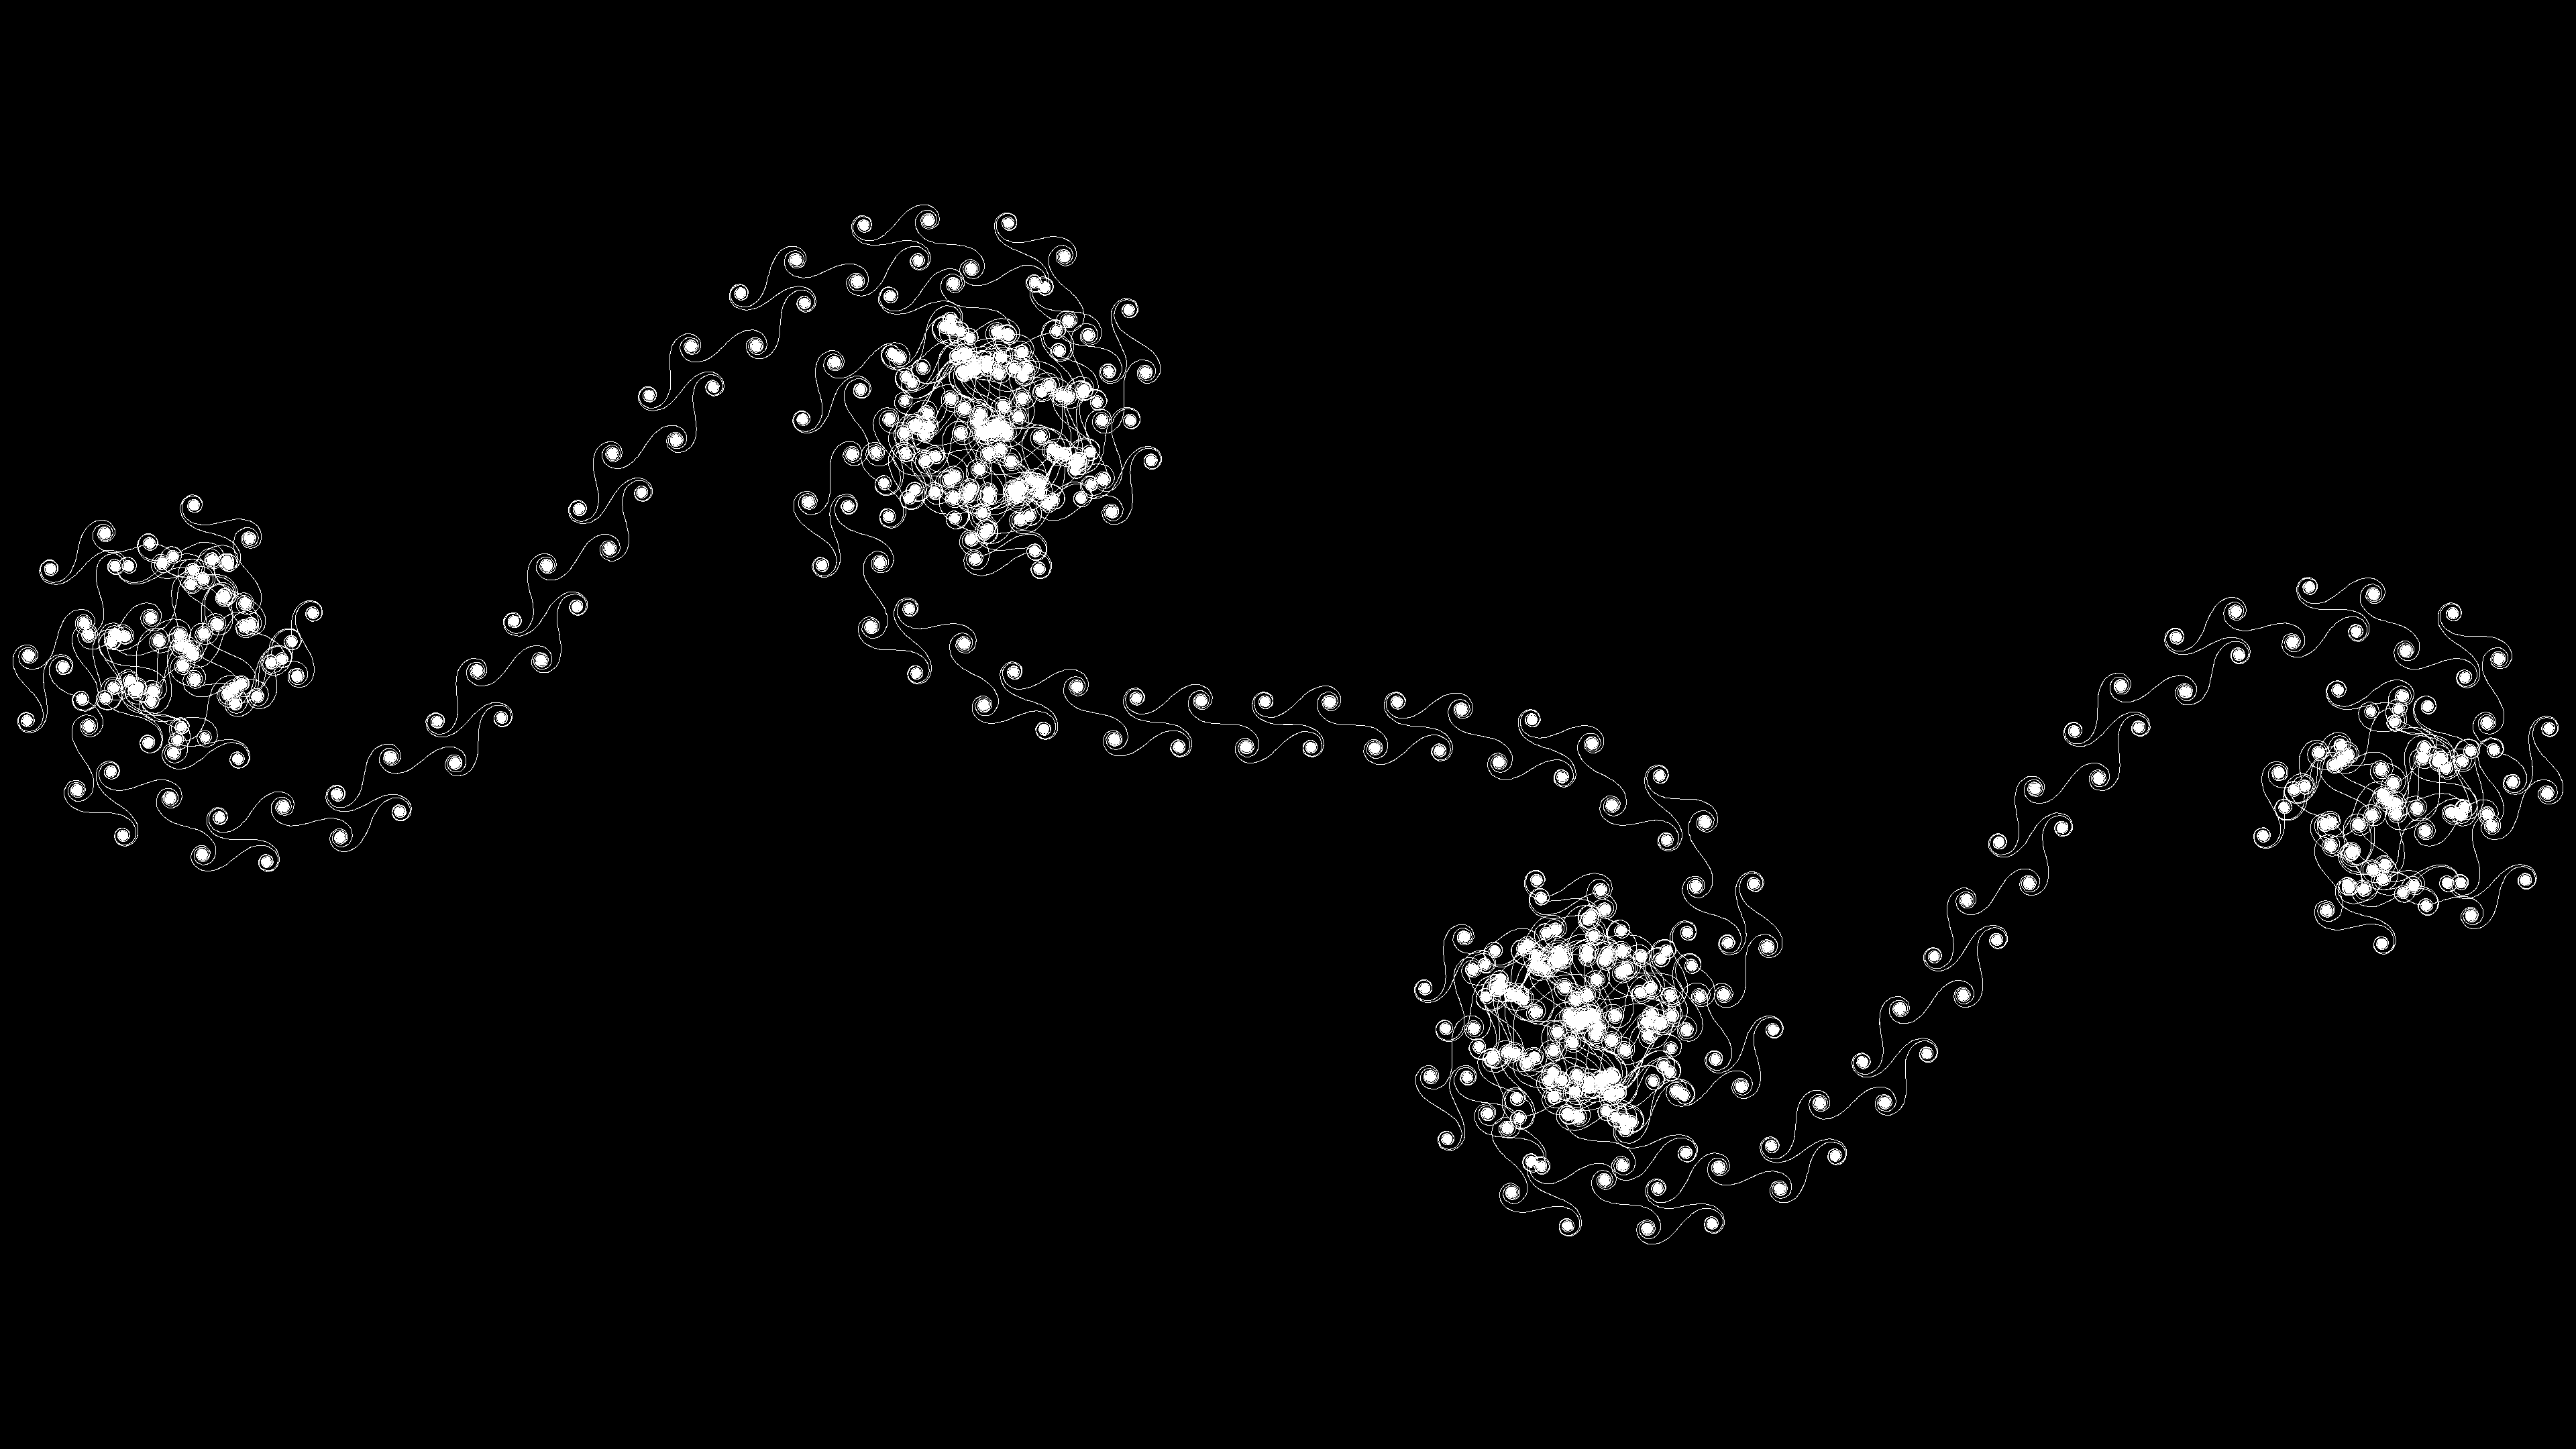
\includegraphics[width=\linewidth]{./stepsplusoneimages/0000000125.png}
    \caption{tf p=499 q=199724 theta=000 89944123.png}
  \end{subfigure}
  \begin{subfigure}[t]{0.48\textwidth}
    \centering
    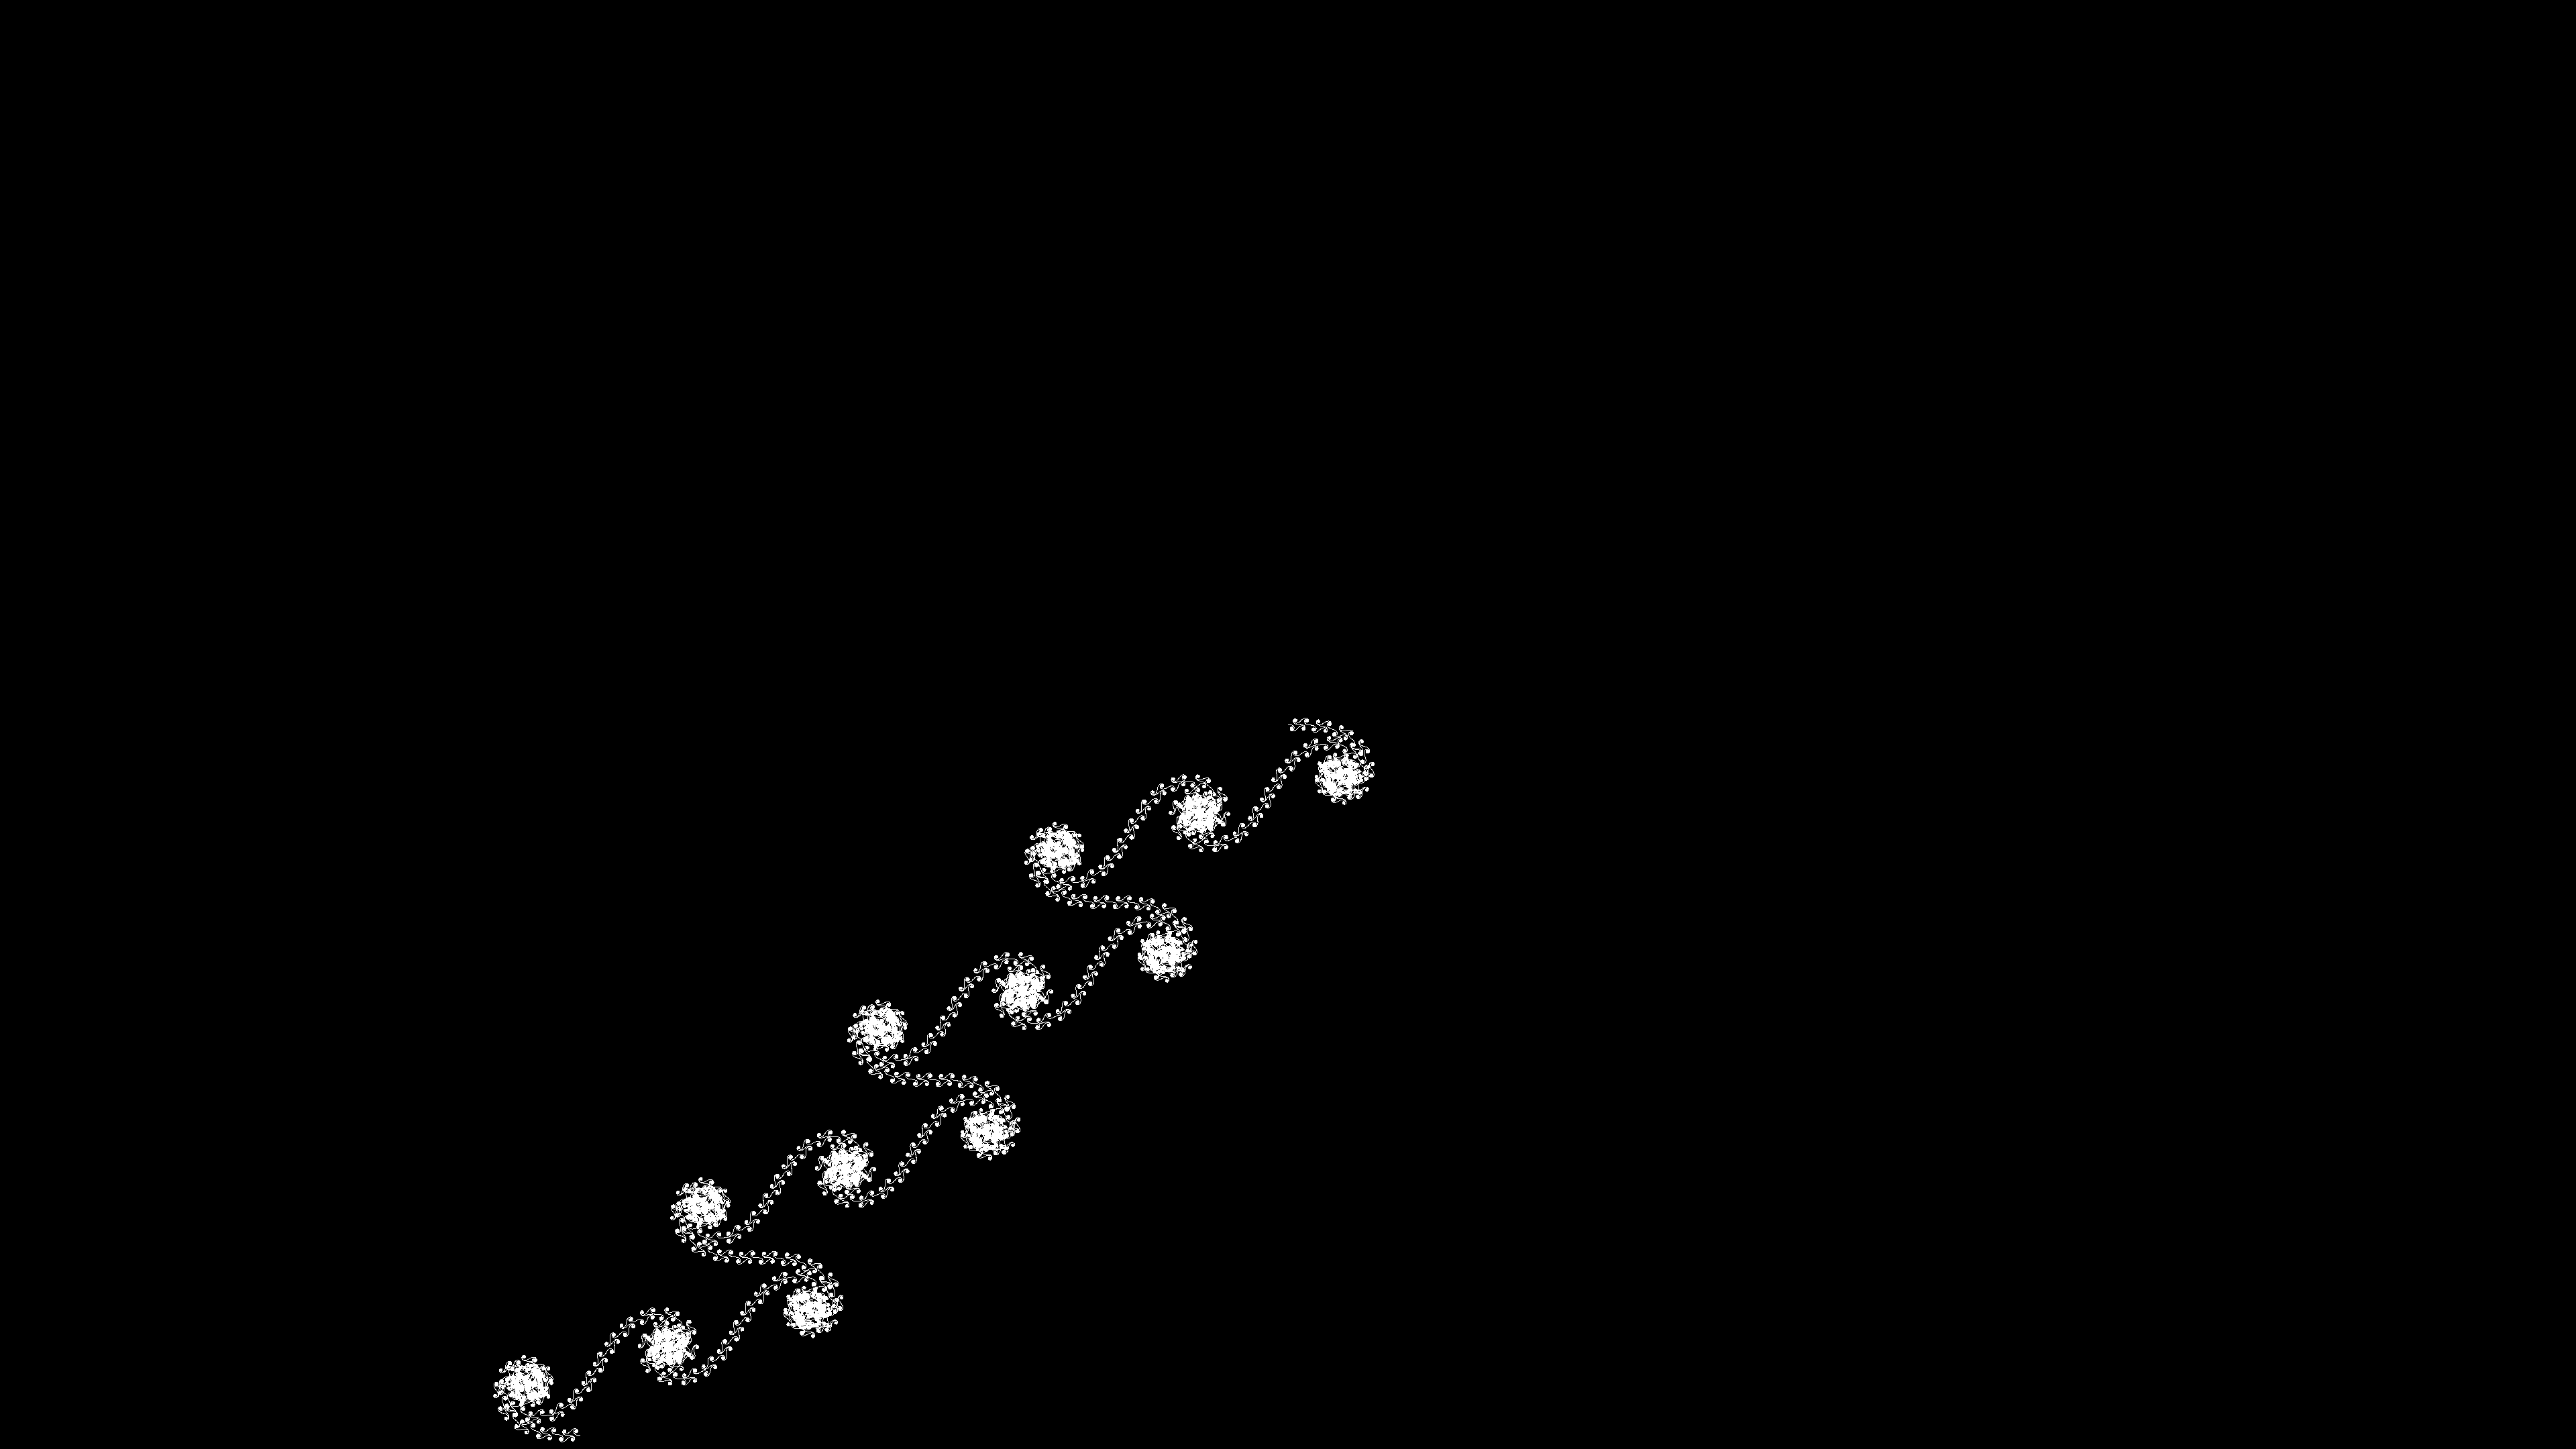
\includegraphics[width=\linewidth]{./stepsplusoneimages/0000000126.png}
    \caption{tf p=499 q=200223 theta=000 89719962.png}
  \end{subfigure}
  \caption{n=124 s=400 s+1=401}
  \label{fig:n=124}
\end{figure}
\begin{figure}[H]
  \centering
  \begin{subfigure}[t]{0.48\textwidth}
    \centering
    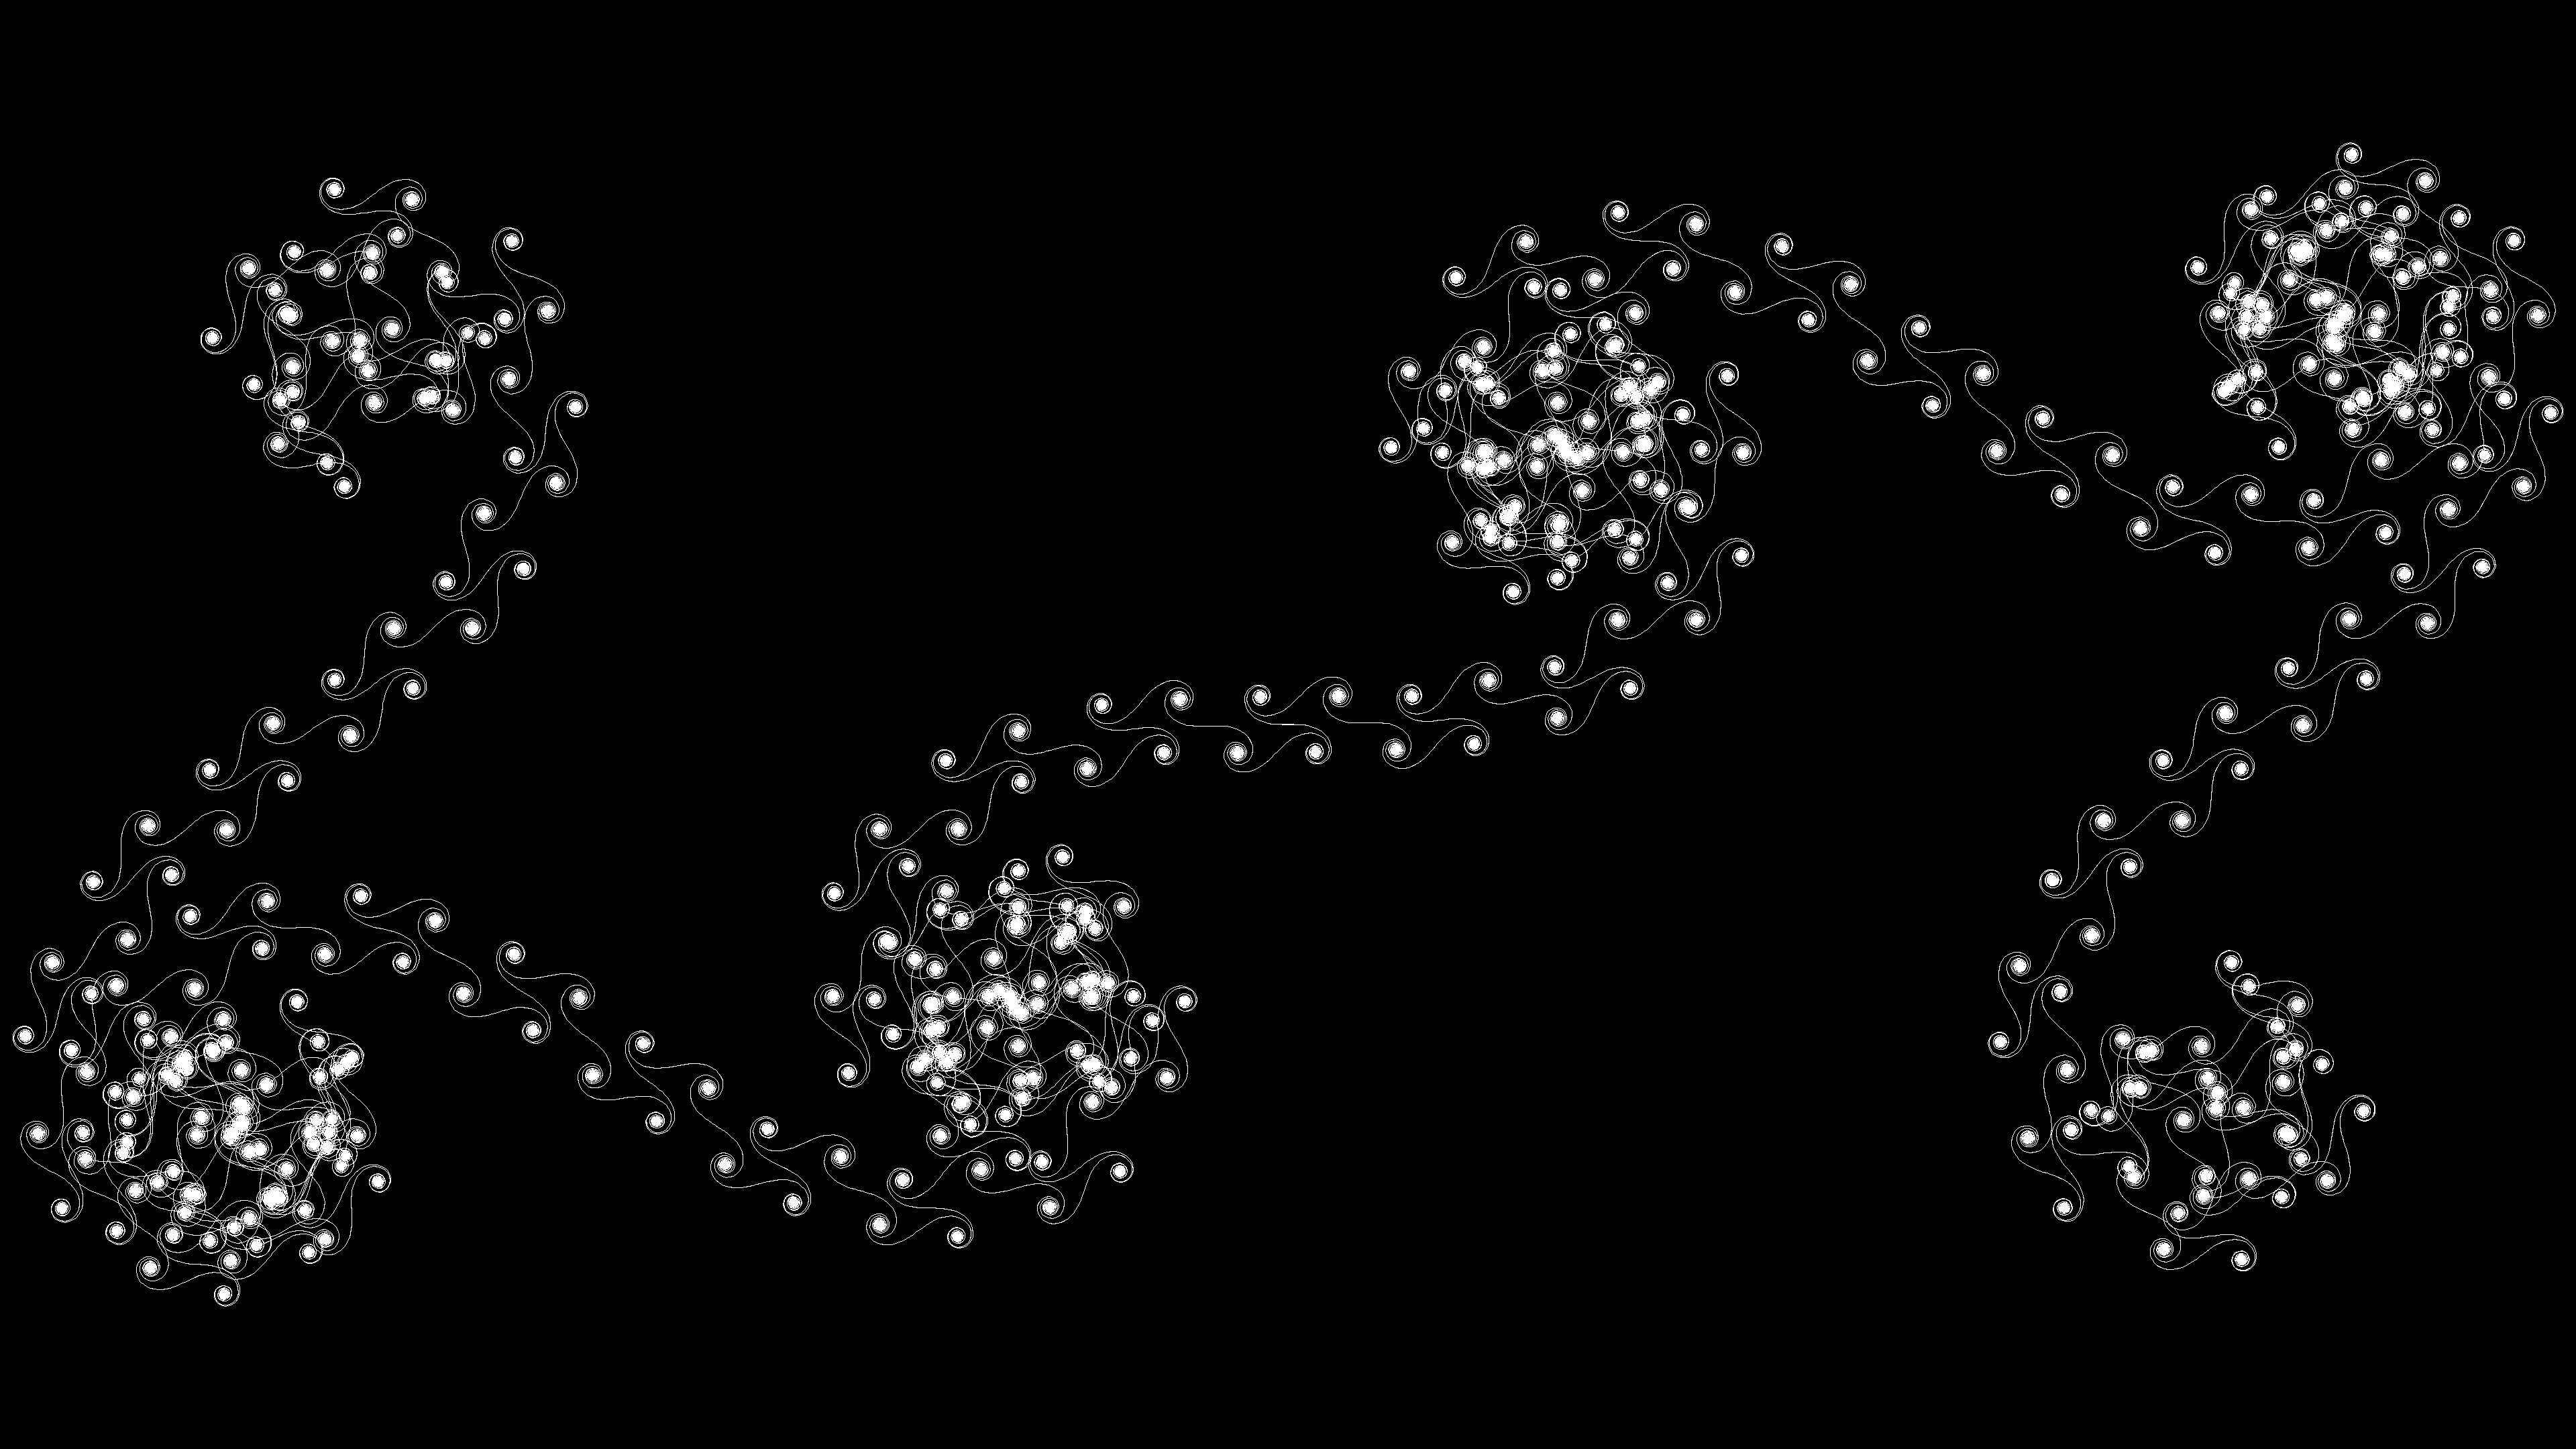
\includegraphics[width=\linewidth]{./stepsplusoneimages/0000000127.png}
    \caption{tf p=499 q=199726 theta=000 89943222.png}
  \end{subfigure}
  \begin{subfigure}[t]{0.48\textwidth}
    \centering
    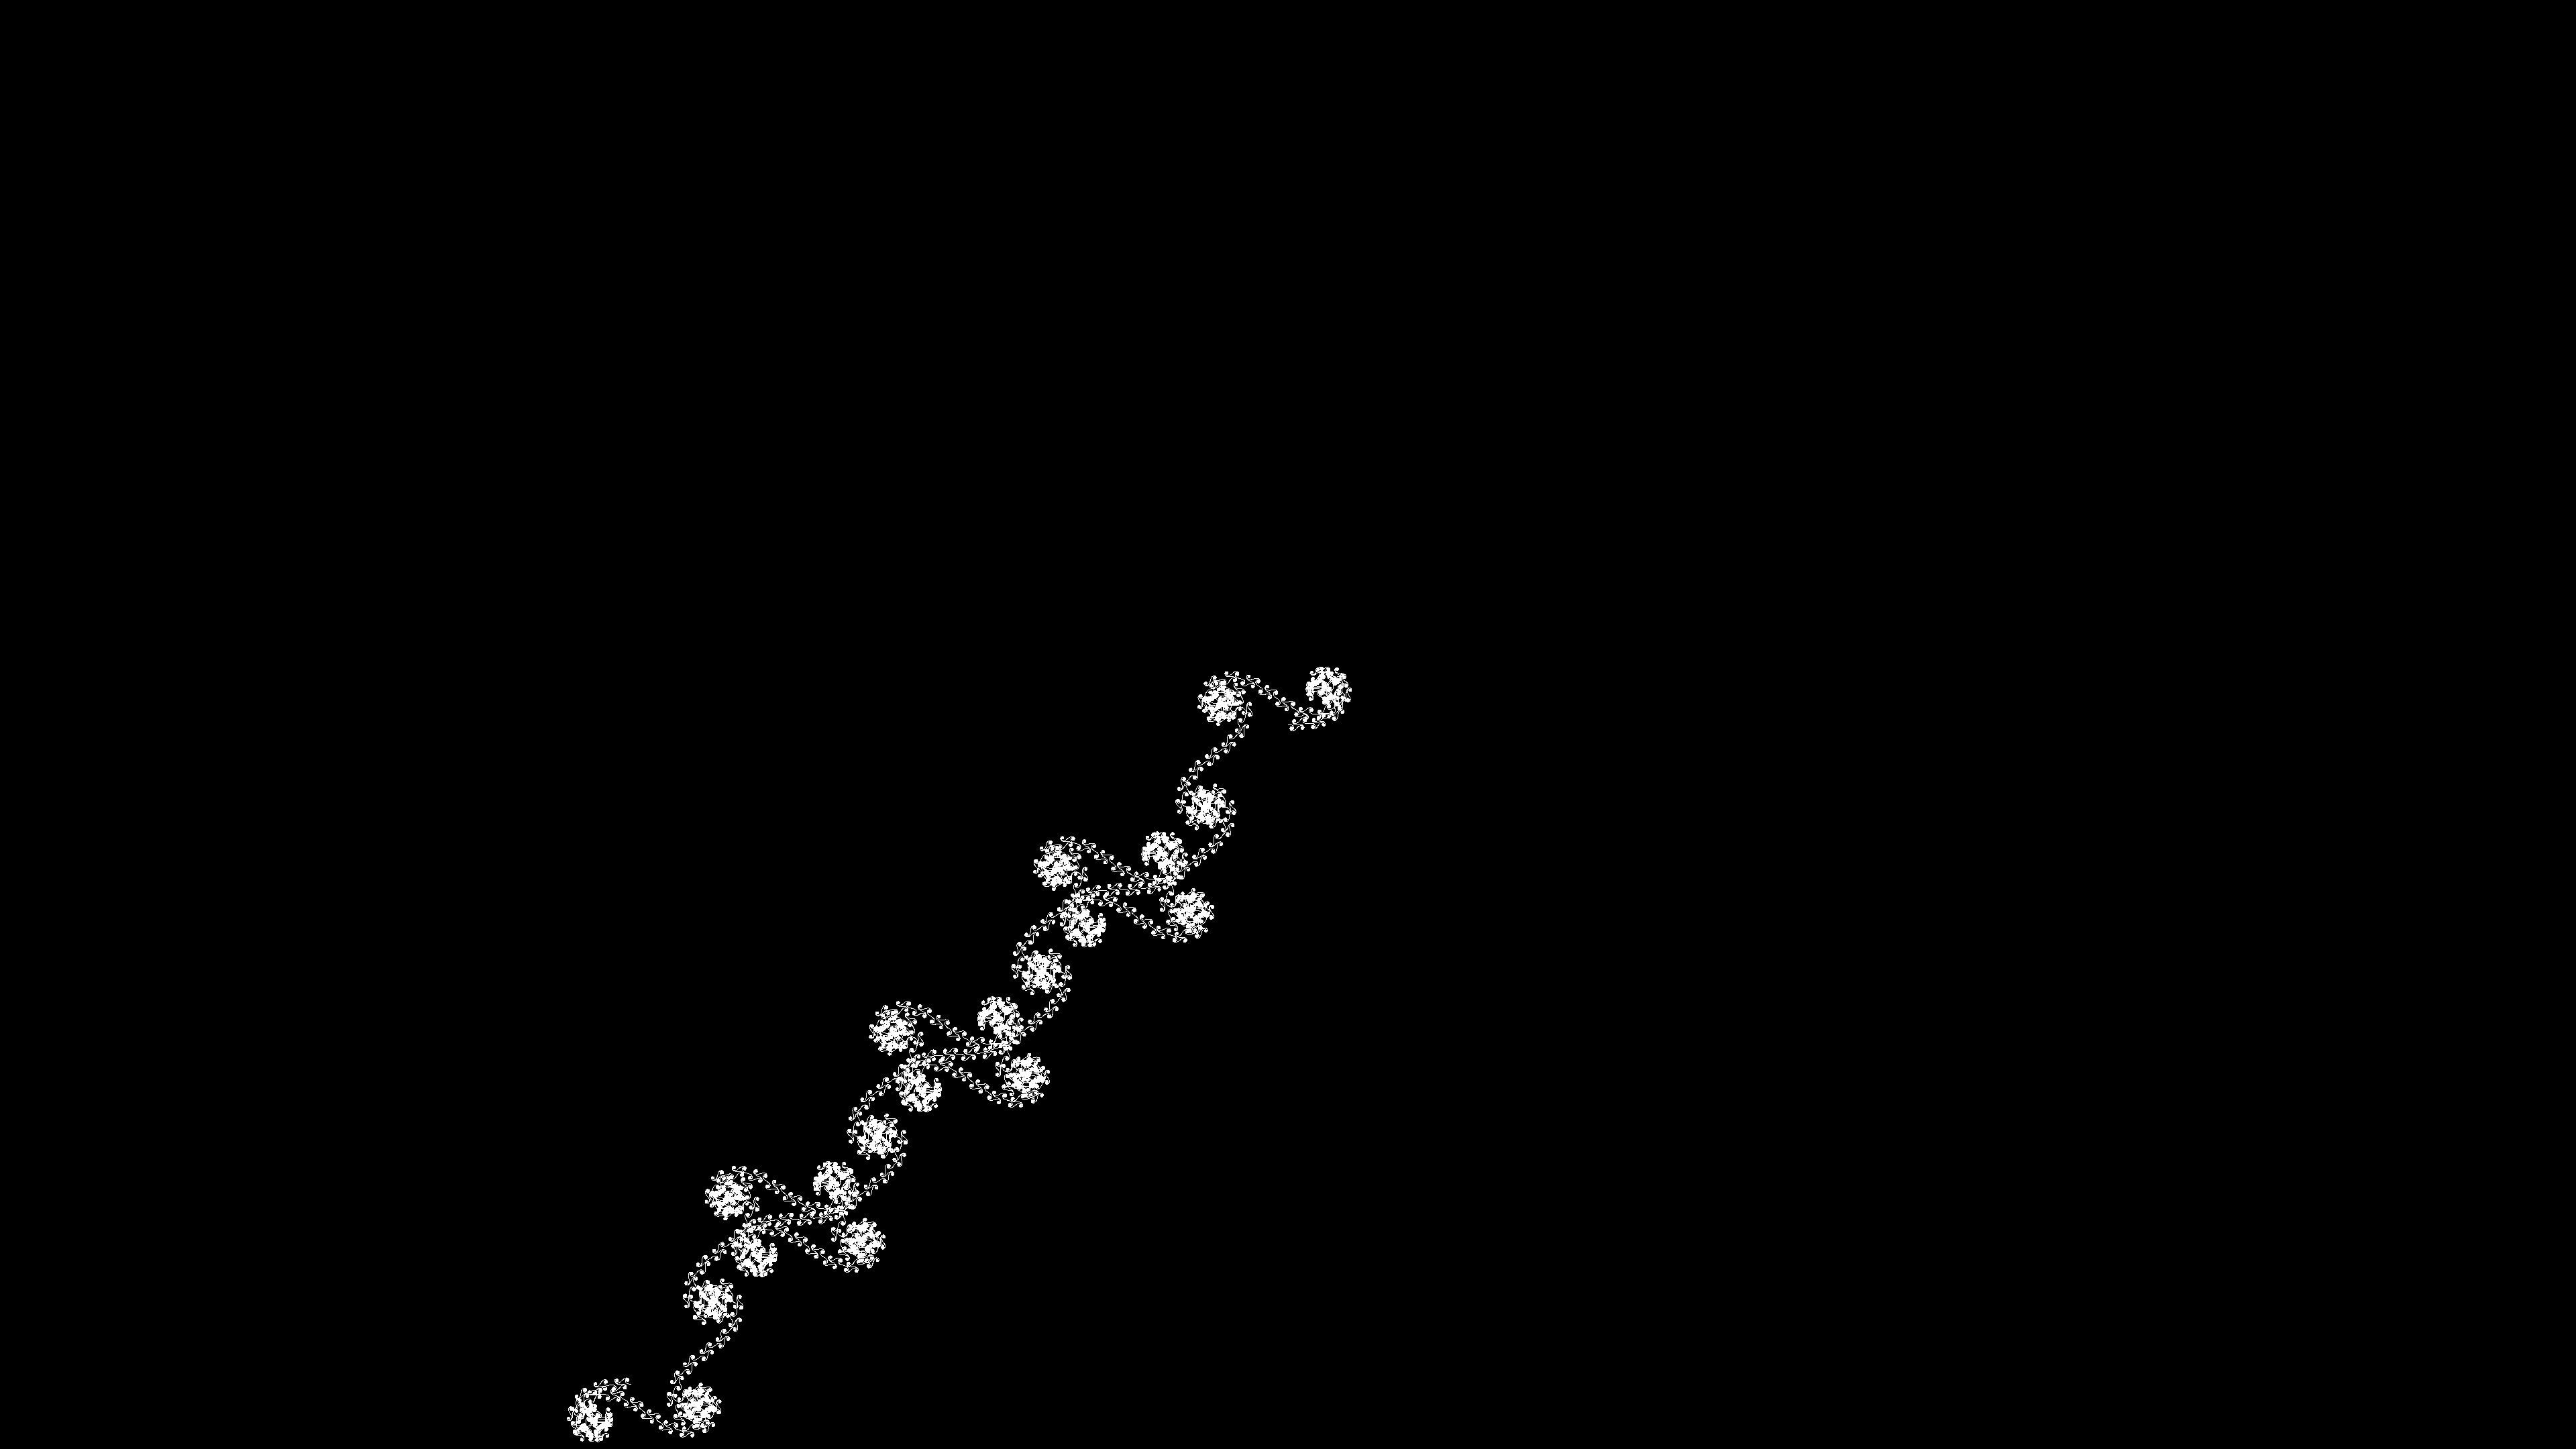
\includegraphics[width=\linewidth]{./stepsplusoneimages/0000000128.png}
    \caption{tf p=499 q=200225 theta=000 89719066.png}
  \end{subfigure}
  \caption{n=126 s=400 s+1=401}
  \label{fig:n=126}
\end{figure}
\begin{figure}[H]
  \centering
  \begin{subfigure}[t]{0.48\textwidth}
    \centering
    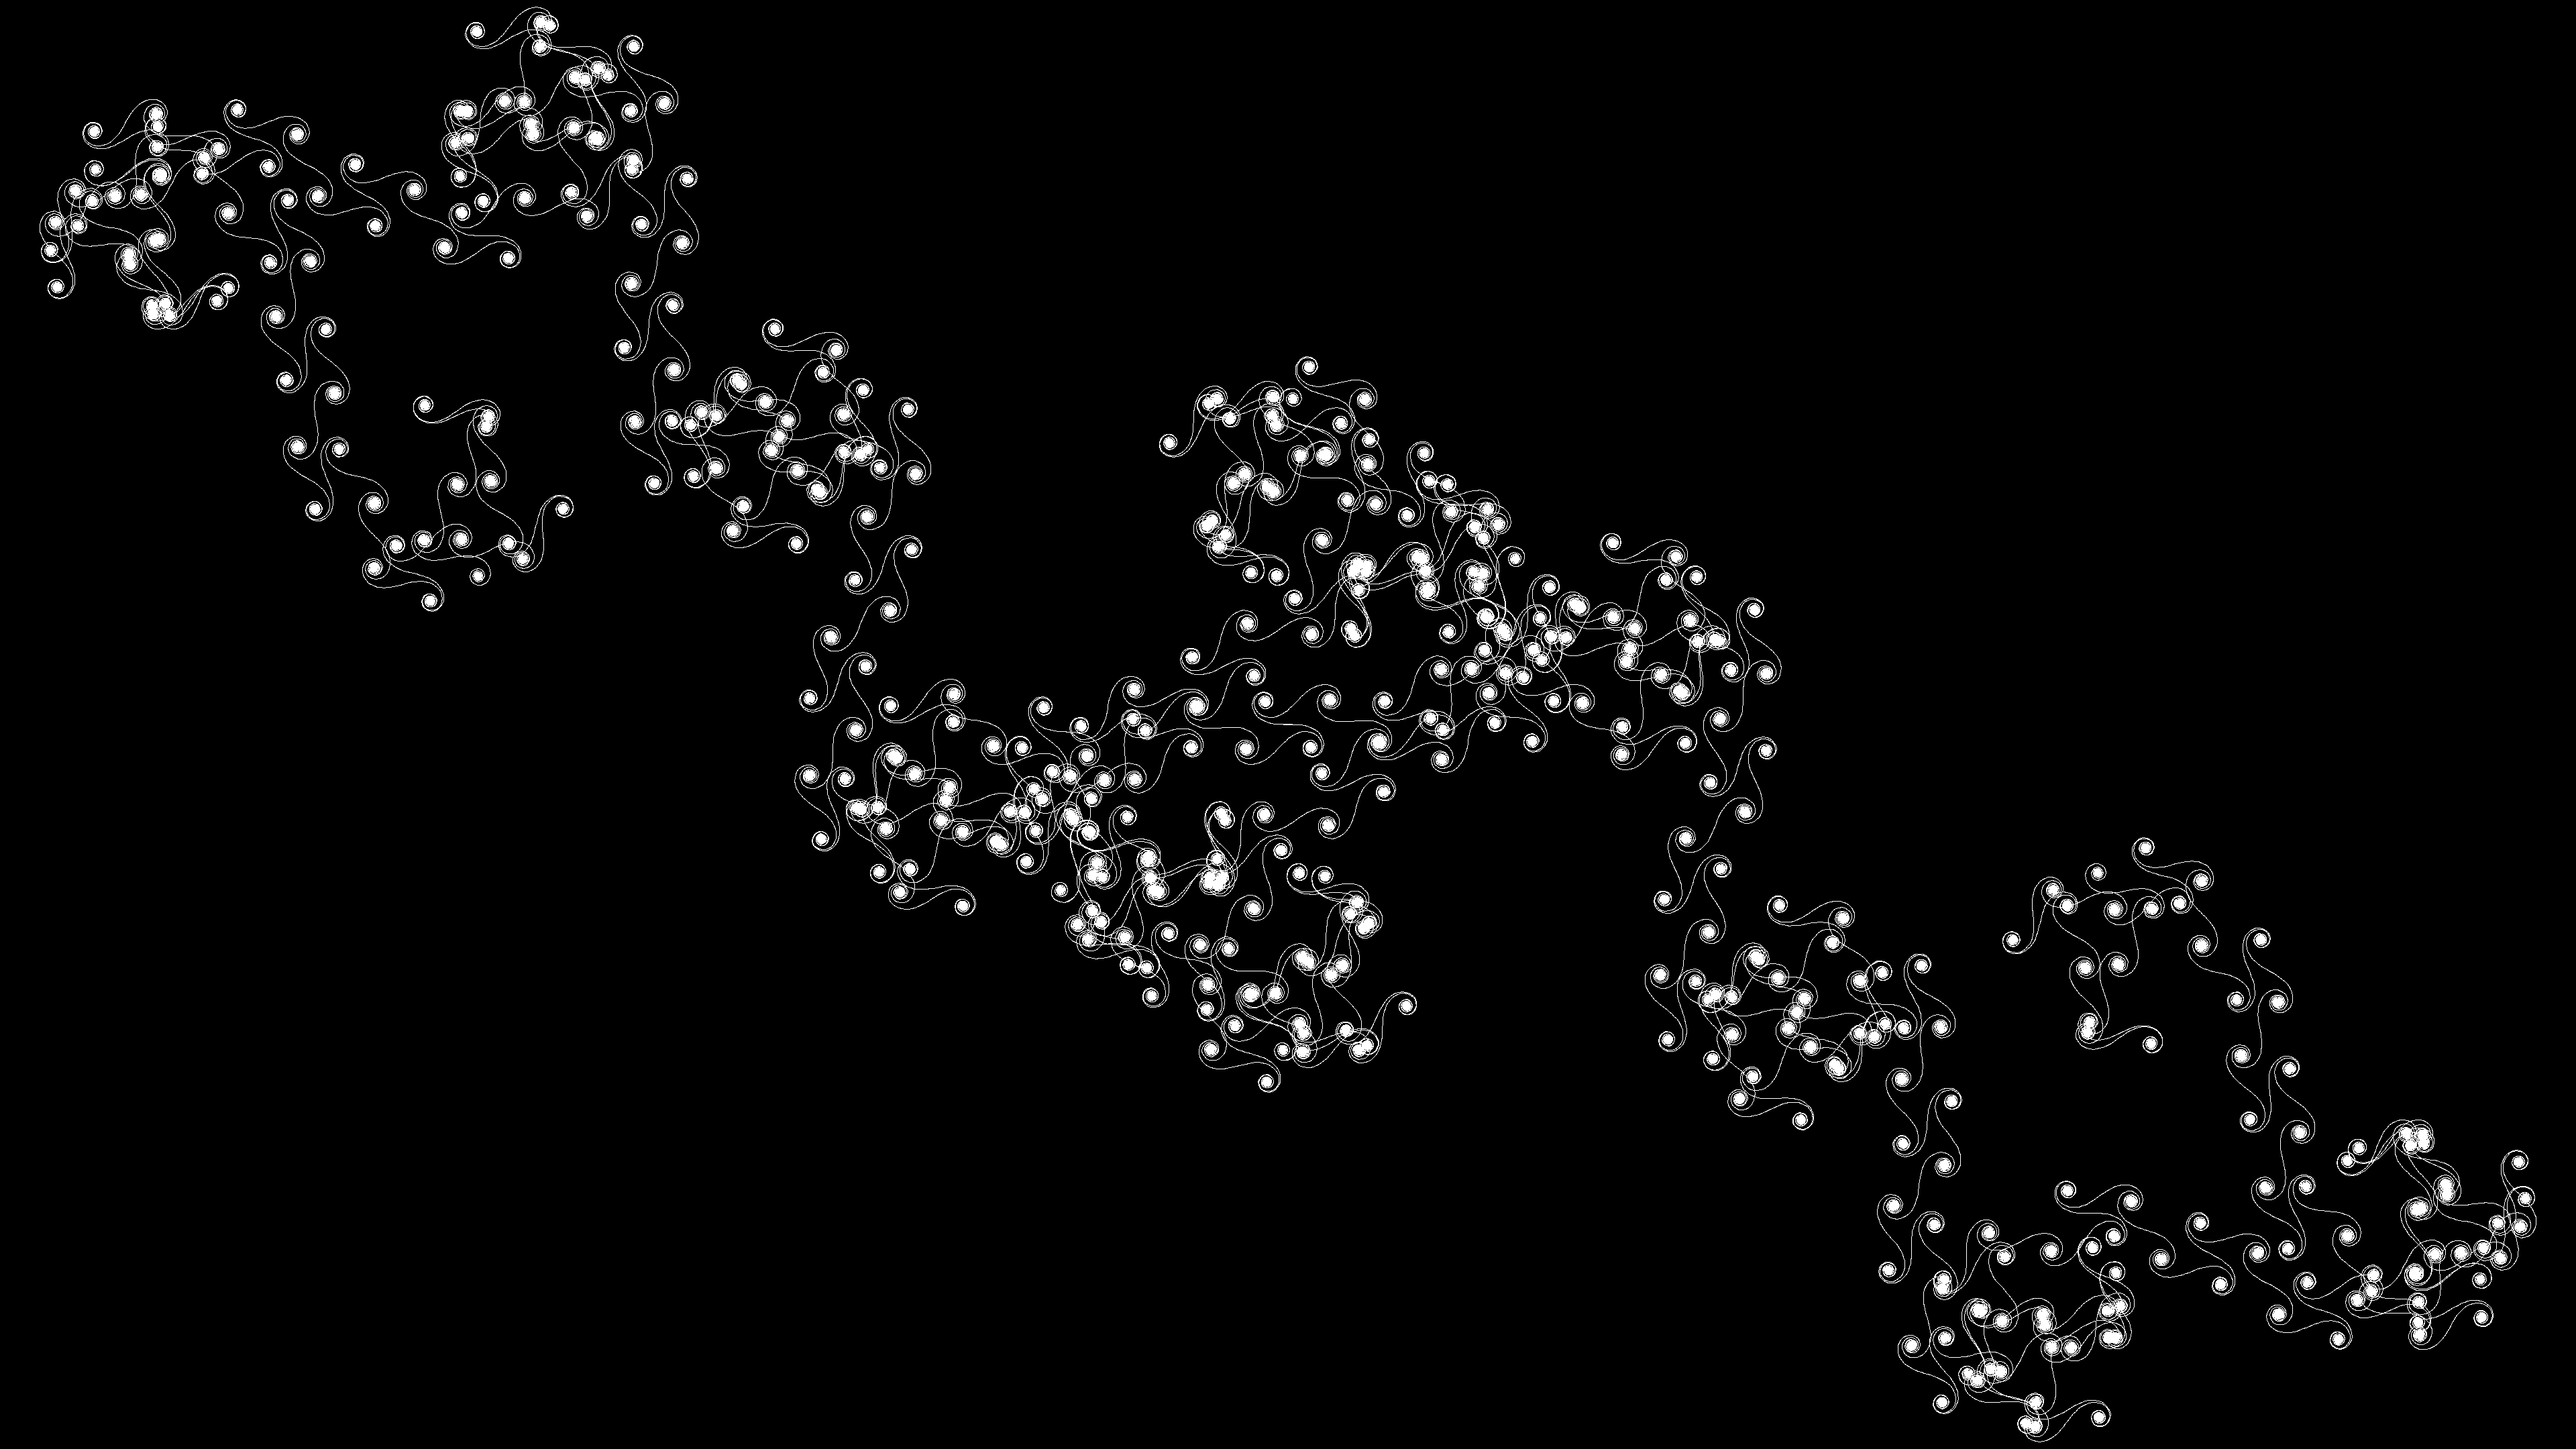
\includegraphics[width=\linewidth]{./stepsplusoneimages/0000000129.png}
    \caption{tf p=499 q=199728 theta=000 89942322.png}
  \end{subfigure}
  \begin{subfigure}[t]{0.48\textwidth}
    \centering
    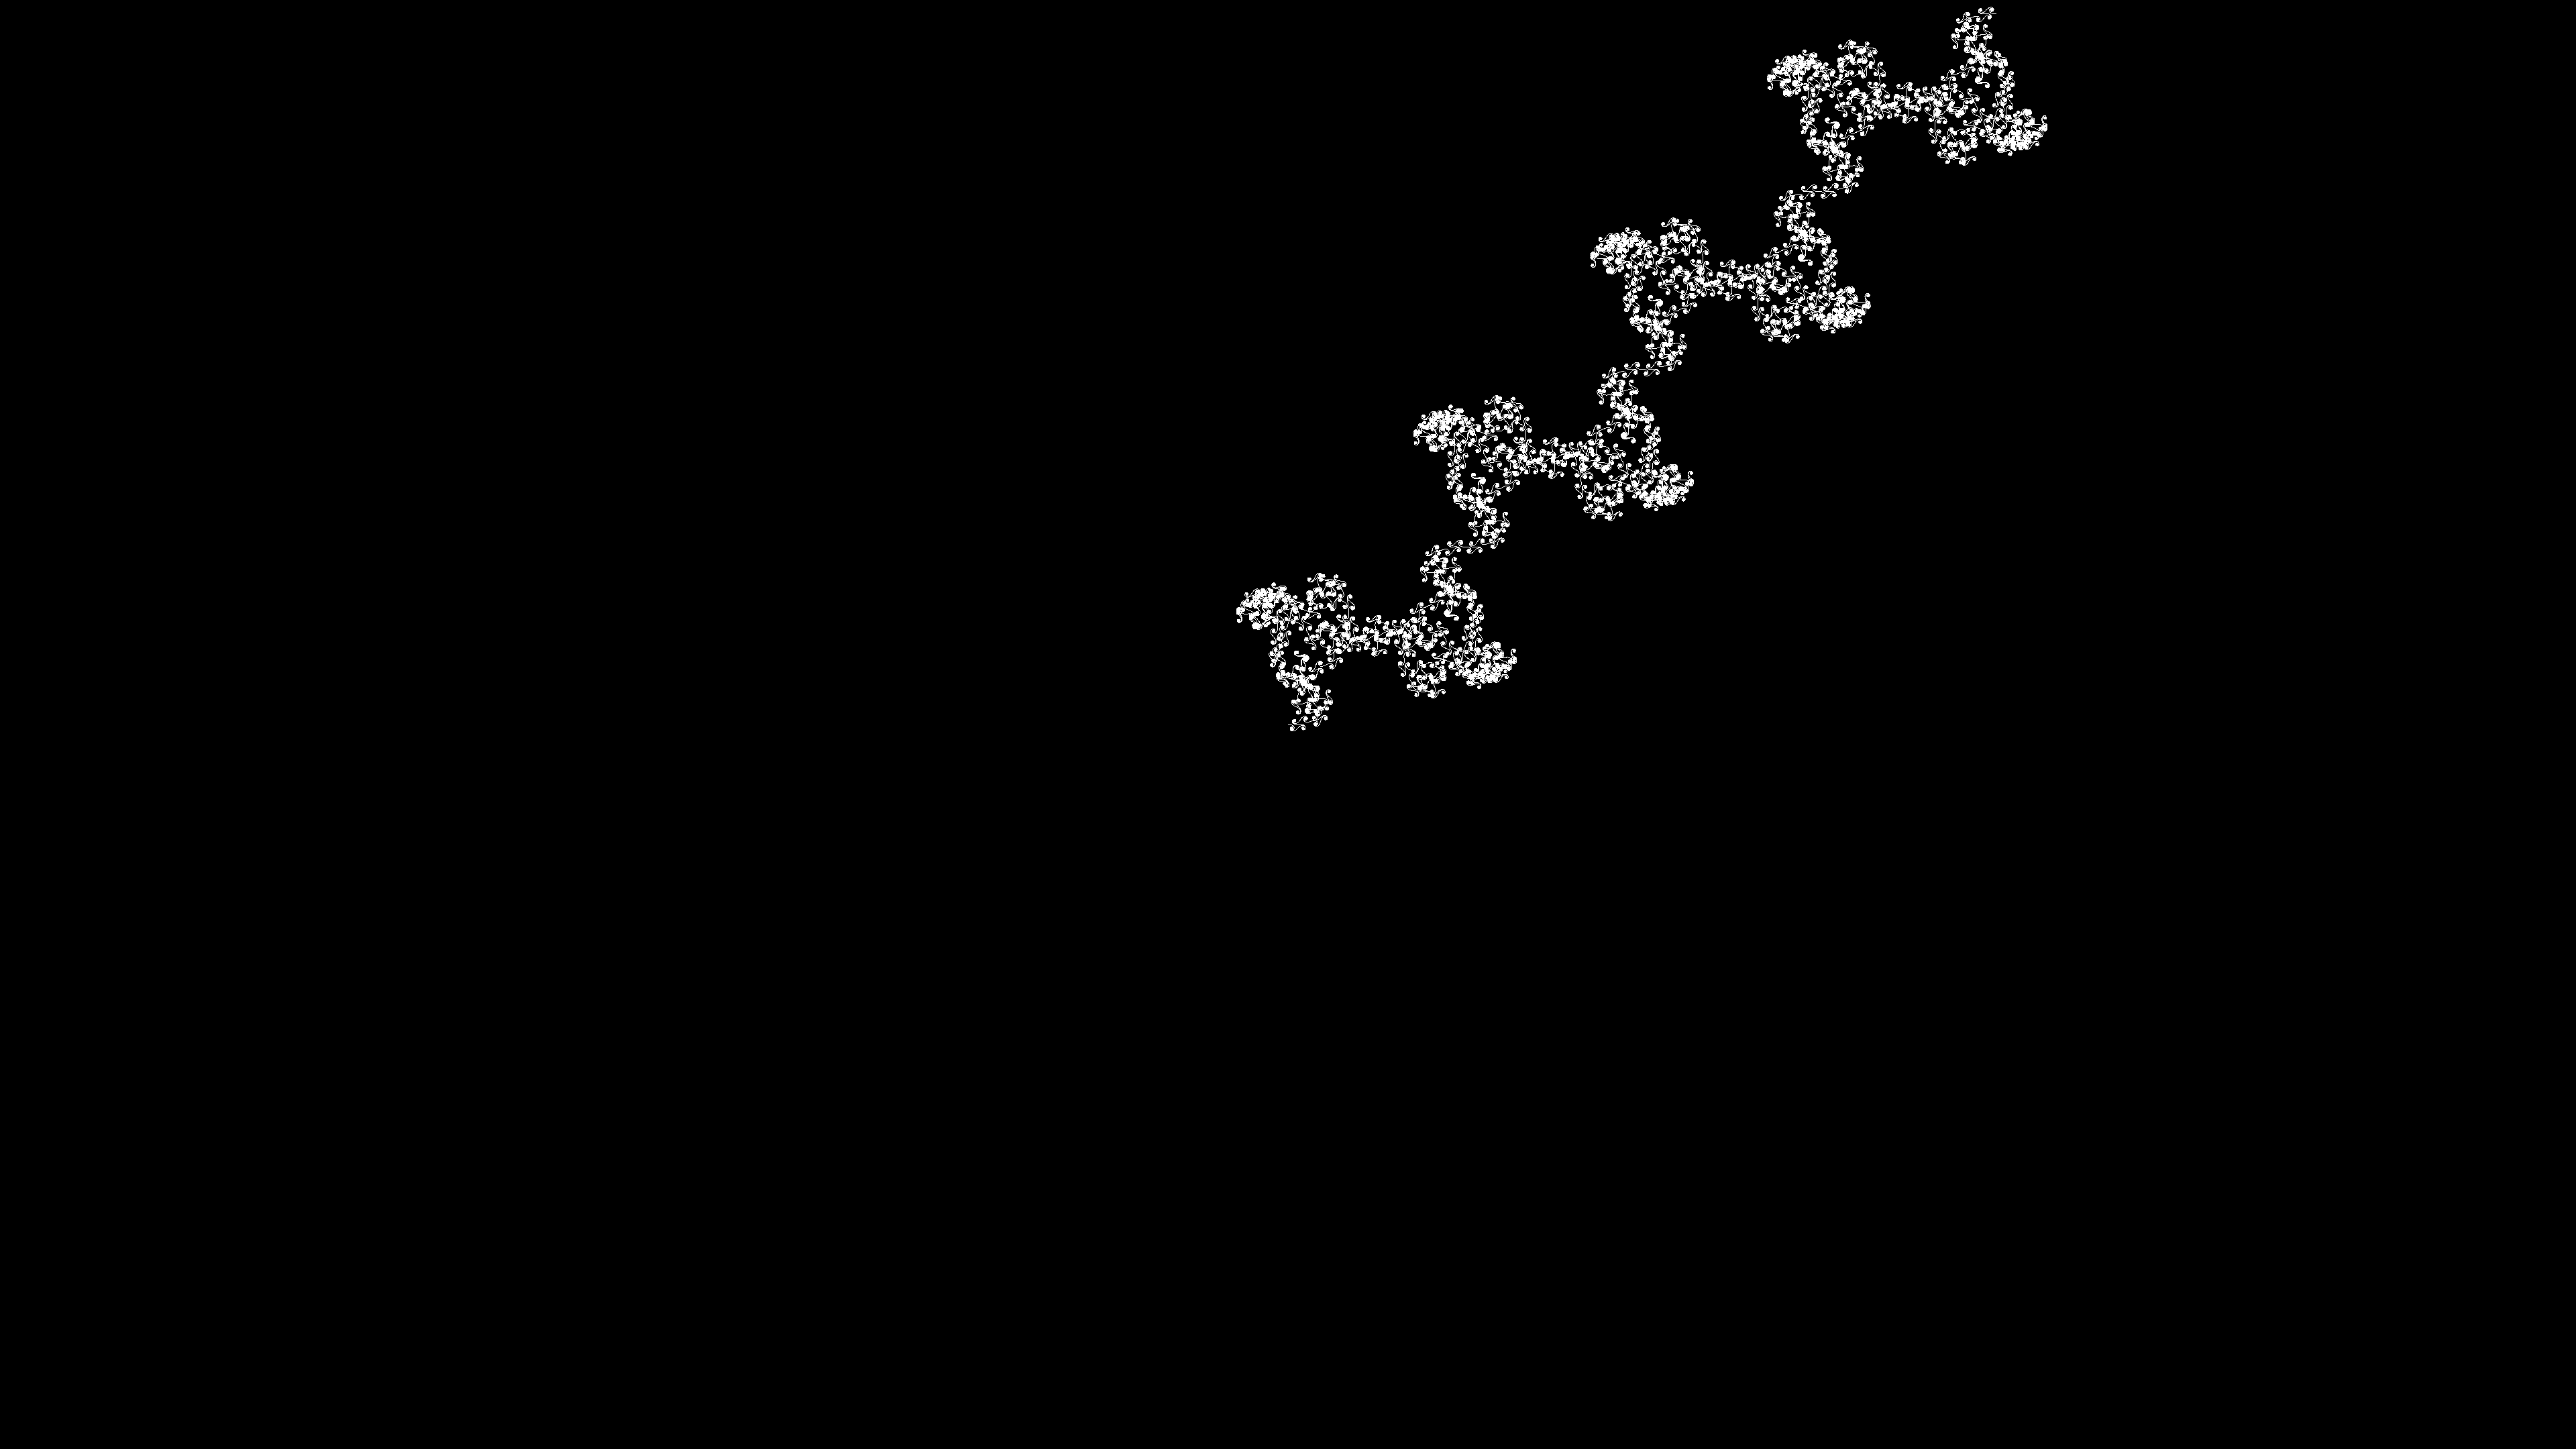
\includegraphics[width=\linewidth]{./stepsplusoneimages/0000000130.png}
    \caption{tf p=499 q=200227 theta=000 89718170.png}
  \end{subfigure}
  \caption{n=128 s=400 s+1=401}
  \label{fig:n=128}
\end{figure}
\begin{figure}[H]
  \centering
  \begin{subfigure}[t]{0.48\textwidth}
    \centering
    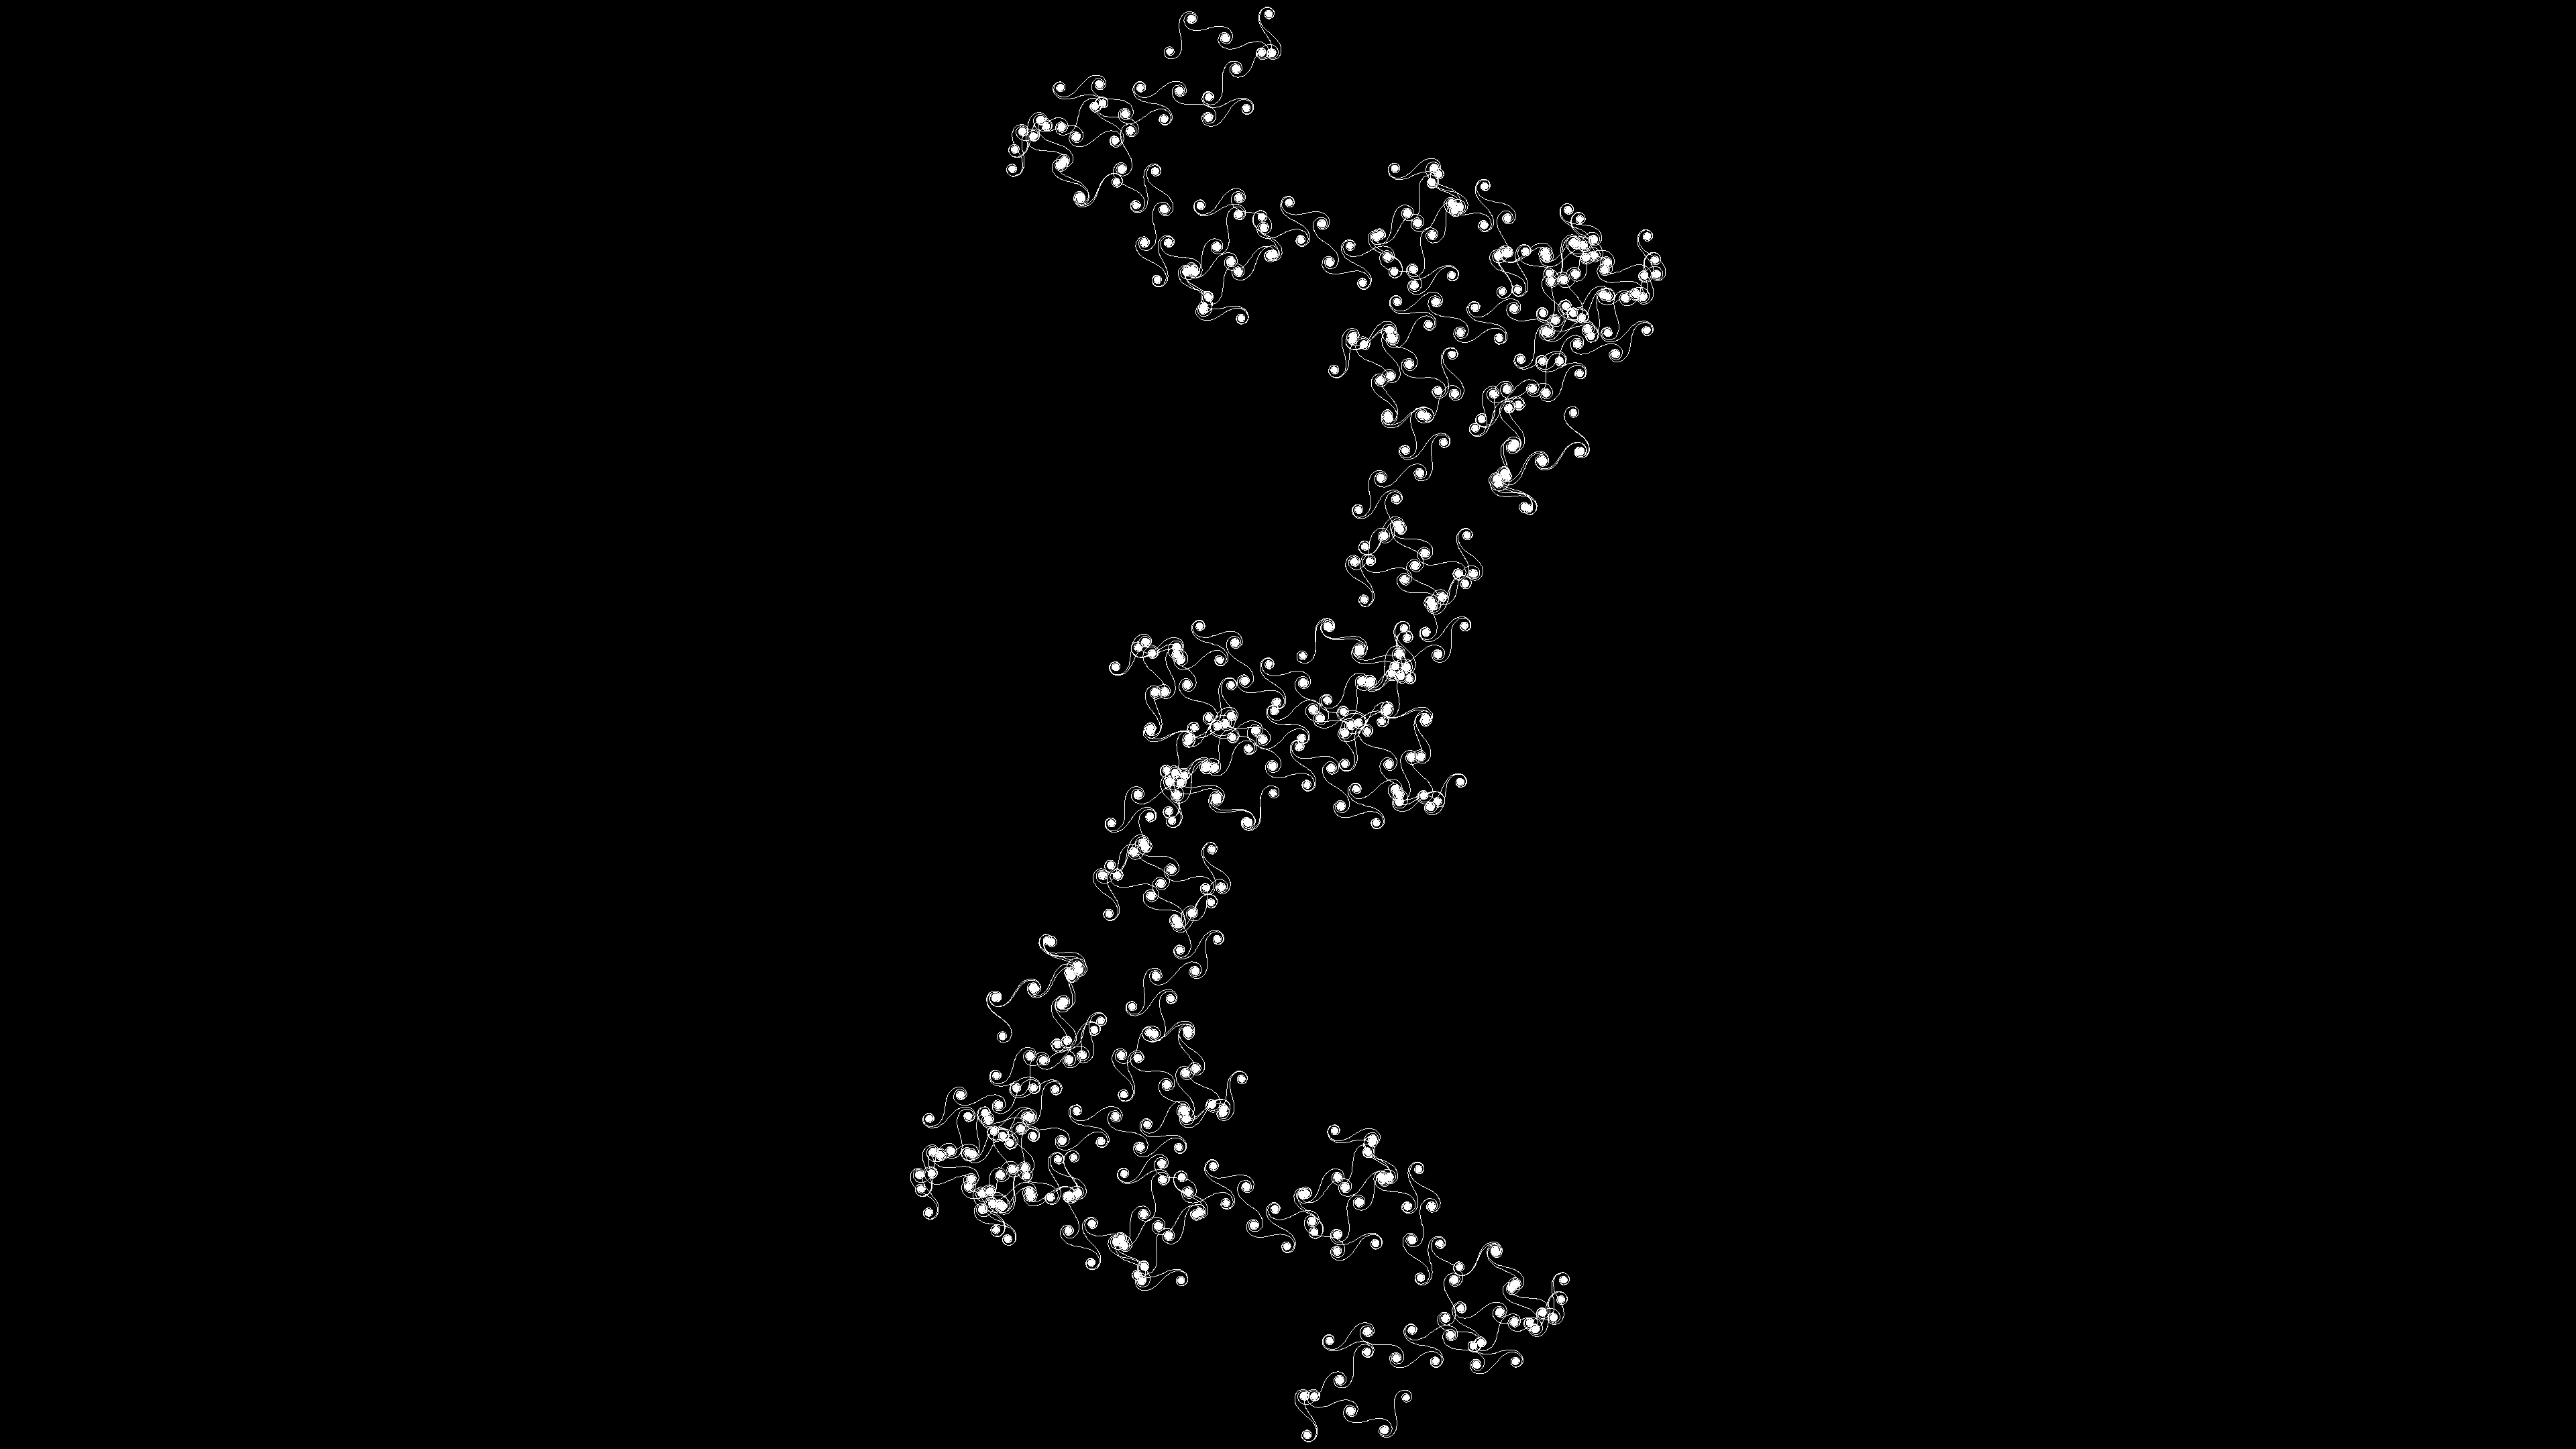
\includegraphics[width=\linewidth]{./stepsplusoneimages/0000000131.png}
    \caption{tf p=499 q=199730 theta=000 89941421.png}
  \end{subfigure}
  \begin{subfigure}[t]{0.48\textwidth}
    \centering
    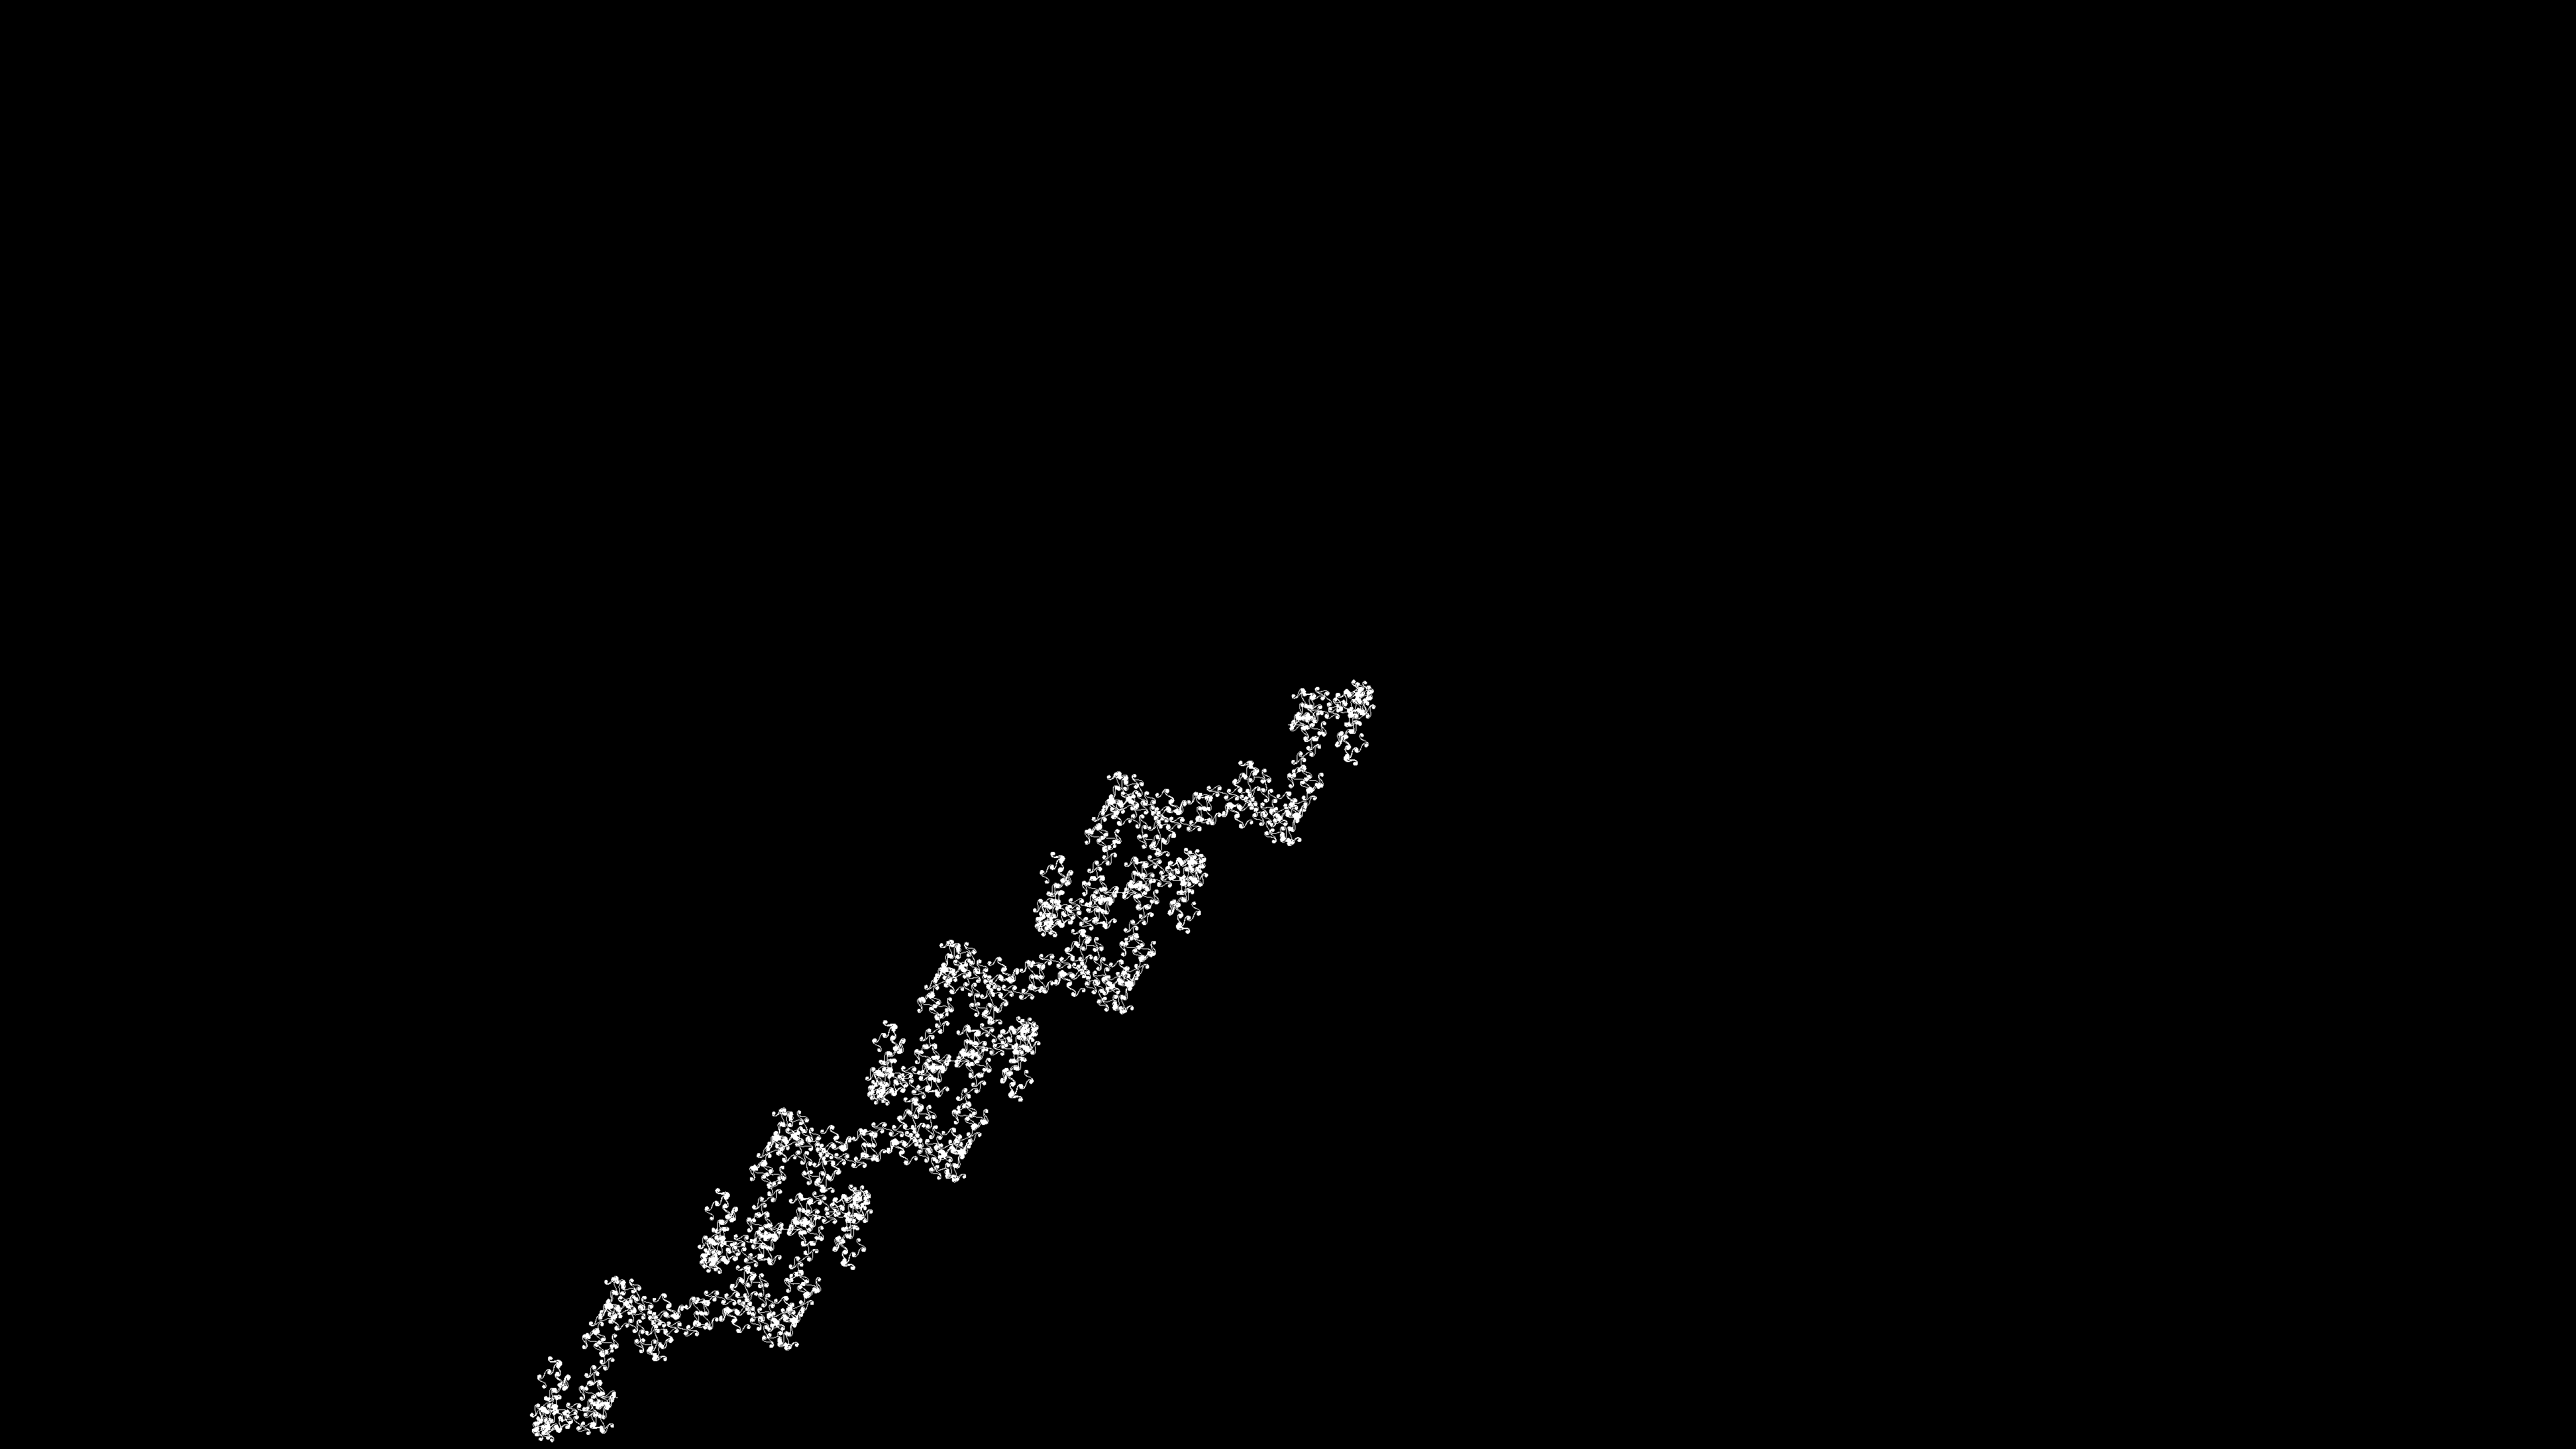
\includegraphics[width=\linewidth]{./stepsplusoneimages/0000000132.png}
    \caption{tf p=499 q=200229 theta=000 89717274.png}
  \end{subfigure}
  \caption{n=130 s=400 s+1=401}
  \label{fig:n=130}
\end{figure}
\begin{figure}[H]
  \centering
  \begin{subfigure}[t]{0.48\textwidth}
    \centering
    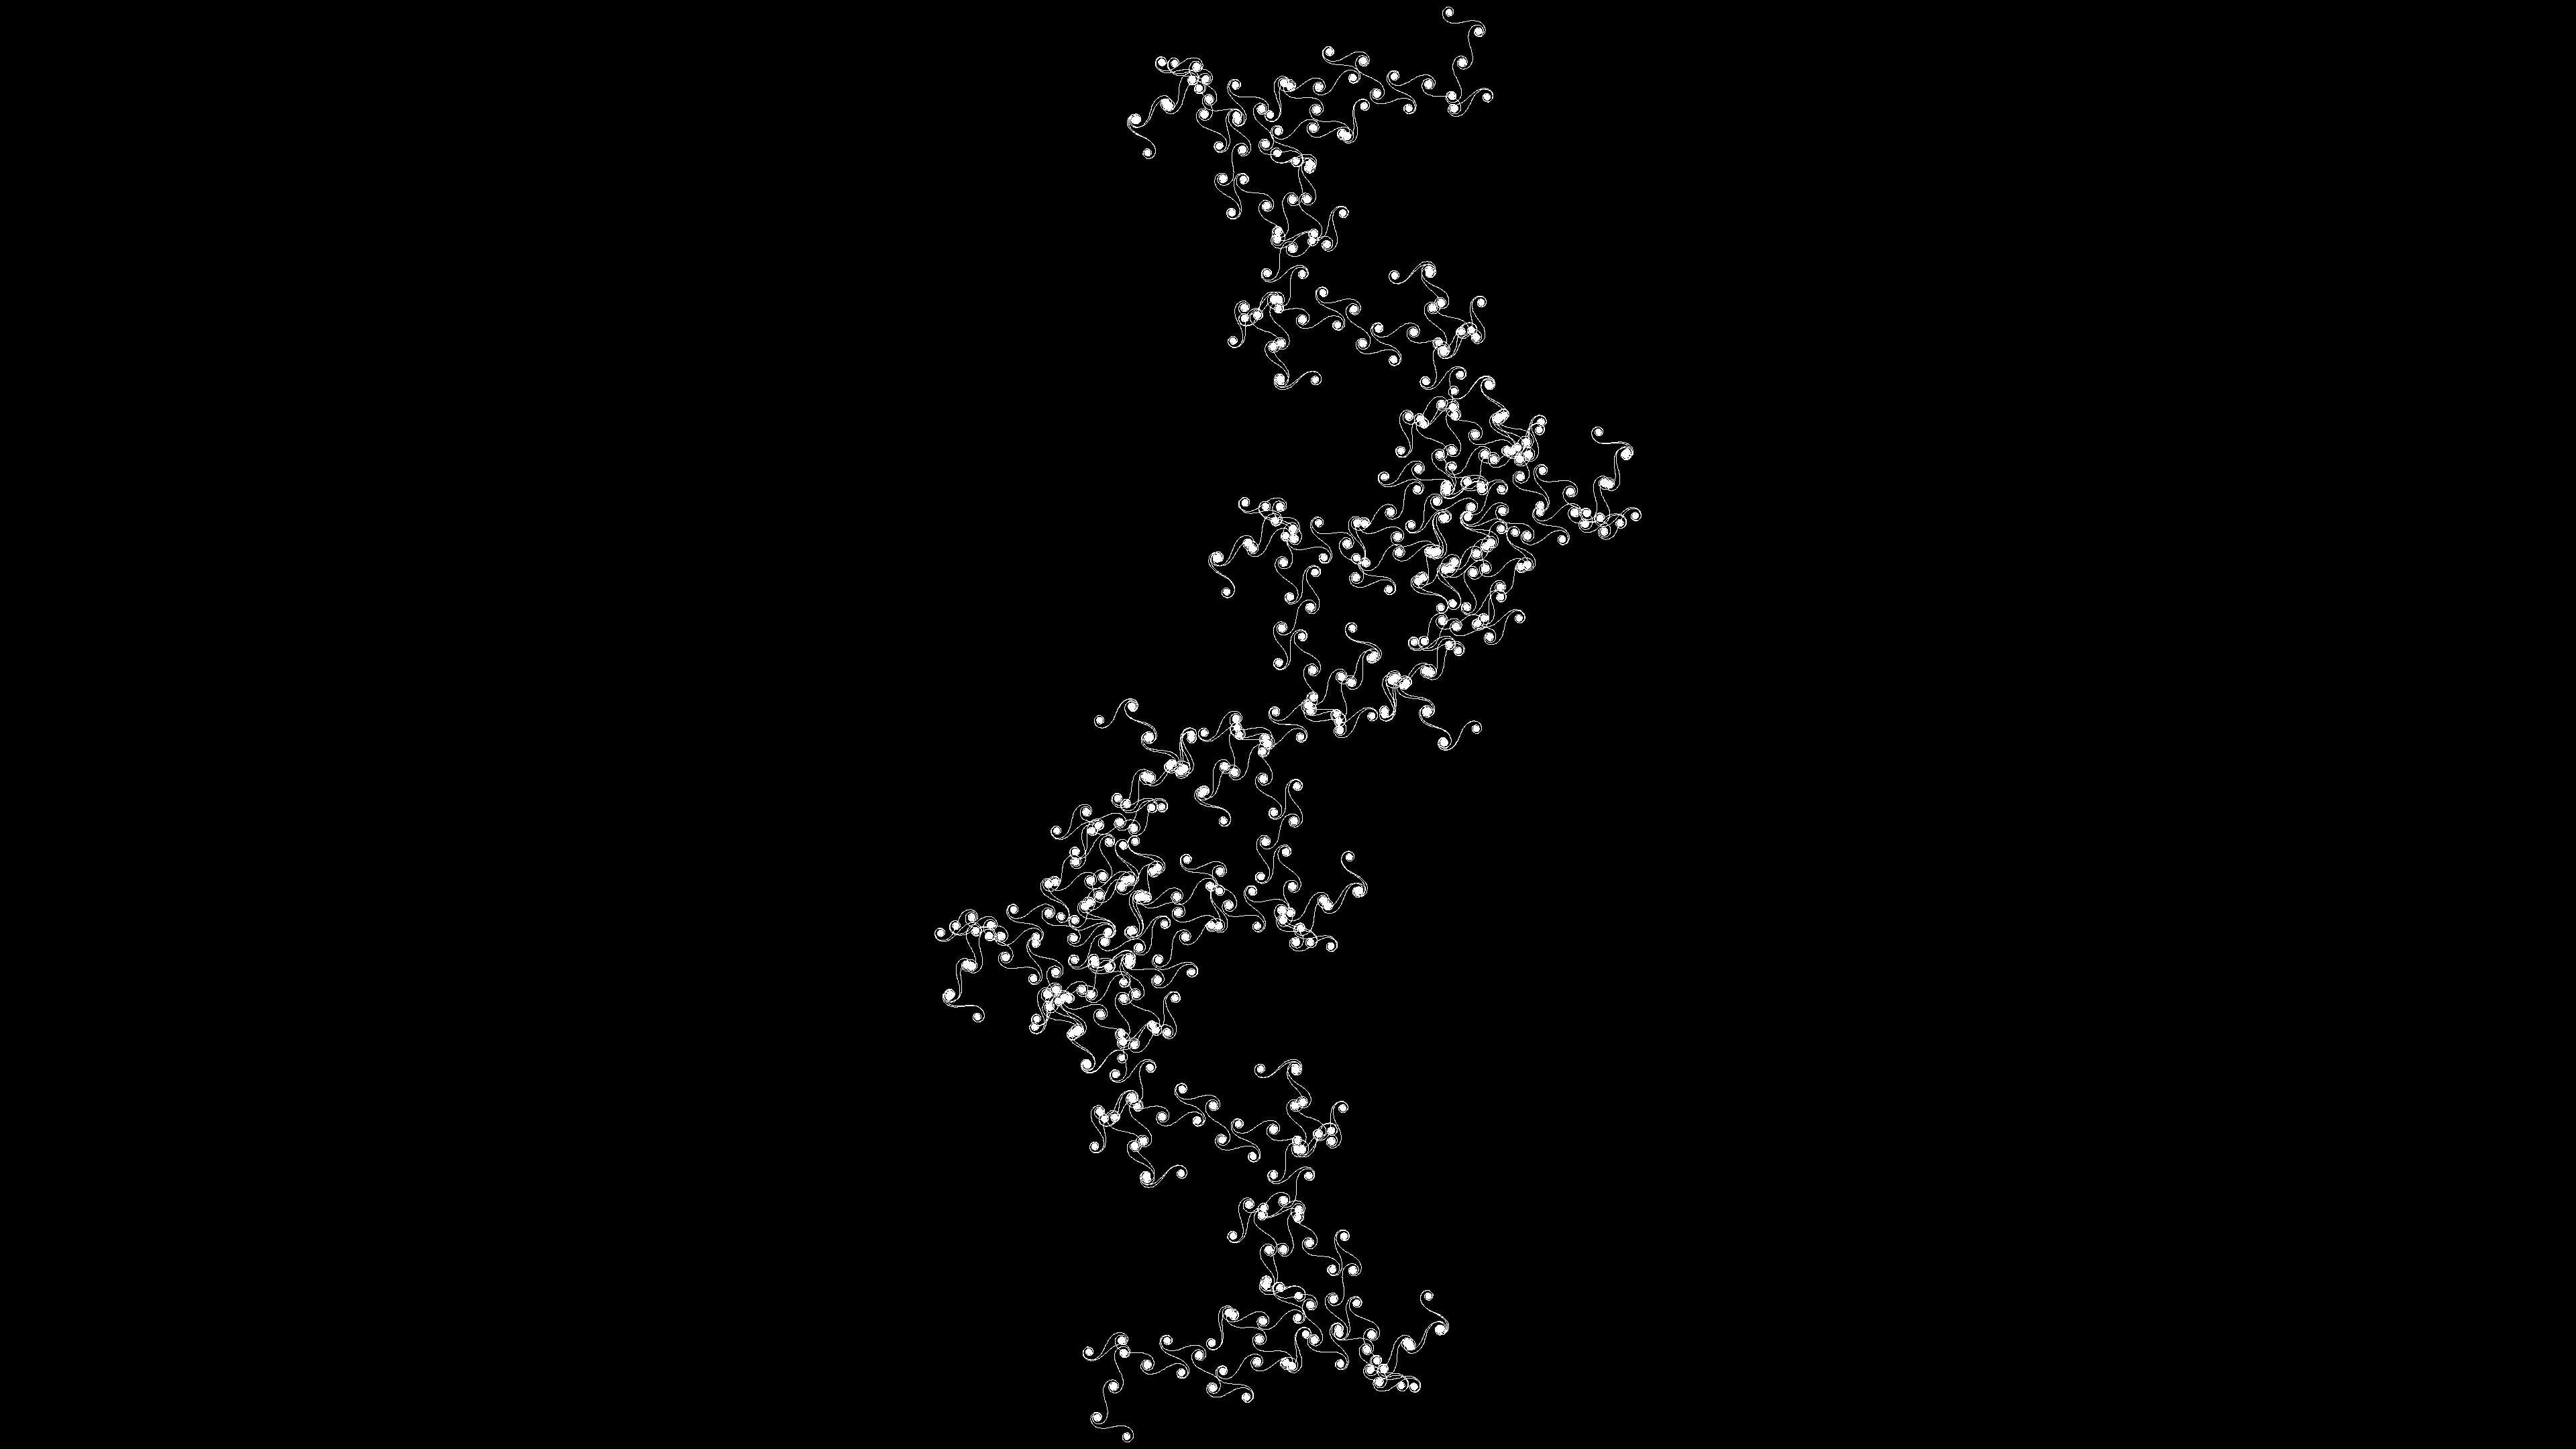
\includegraphics[width=\linewidth]{./stepsplusoneimages/0000000133.png}
    \caption{tf p=499 q=199732 theta=000 89940520.png}
  \end{subfigure}
  \begin{subfigure}[t]{0.48\textwidth}
    \centering
    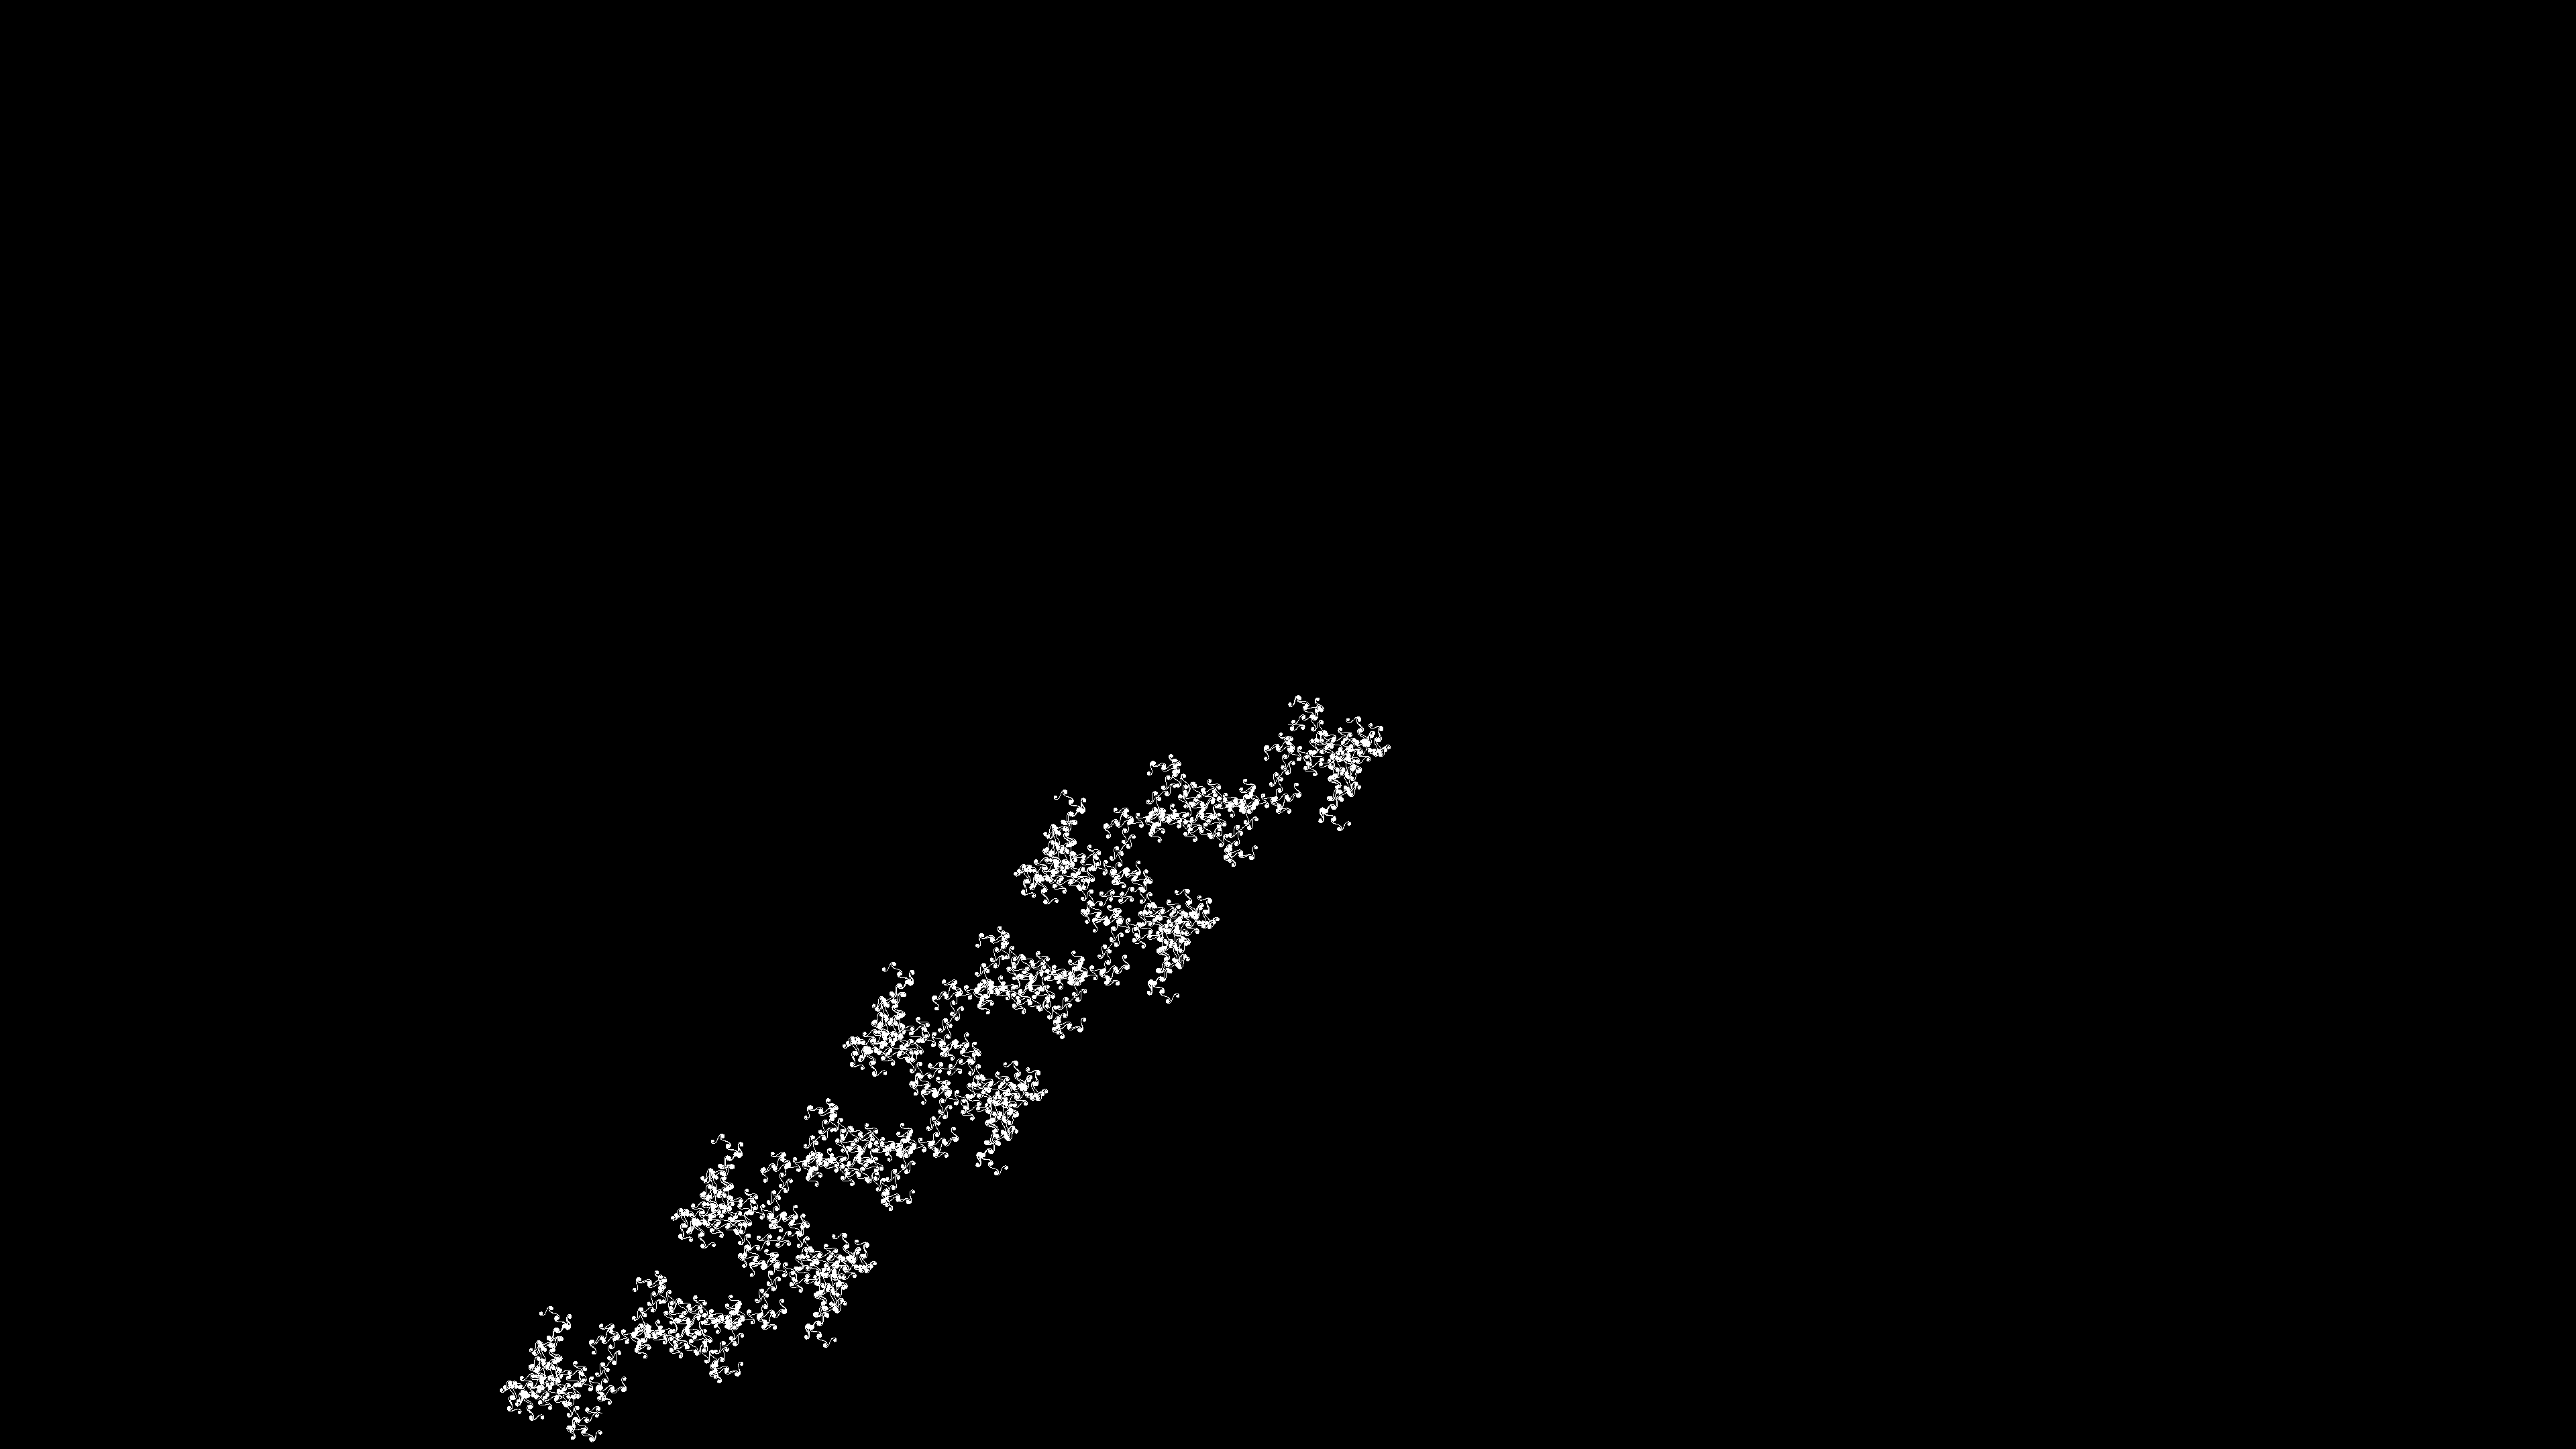
\includegraphics[width=\linewidth]{./stepsplusoneimages/0000000134.png}
    \caption{tf p=499 q=200231 theta=000 89716378.png}
  \end{subfigure}
  \caption{n=132 s=400 s+1=401}
  \label{fig:n=132}
\end{figure}
\begin{figure}[H]
  \centering
  \begin{subfigure}[t]{0.48\textwidth}
    \centering
    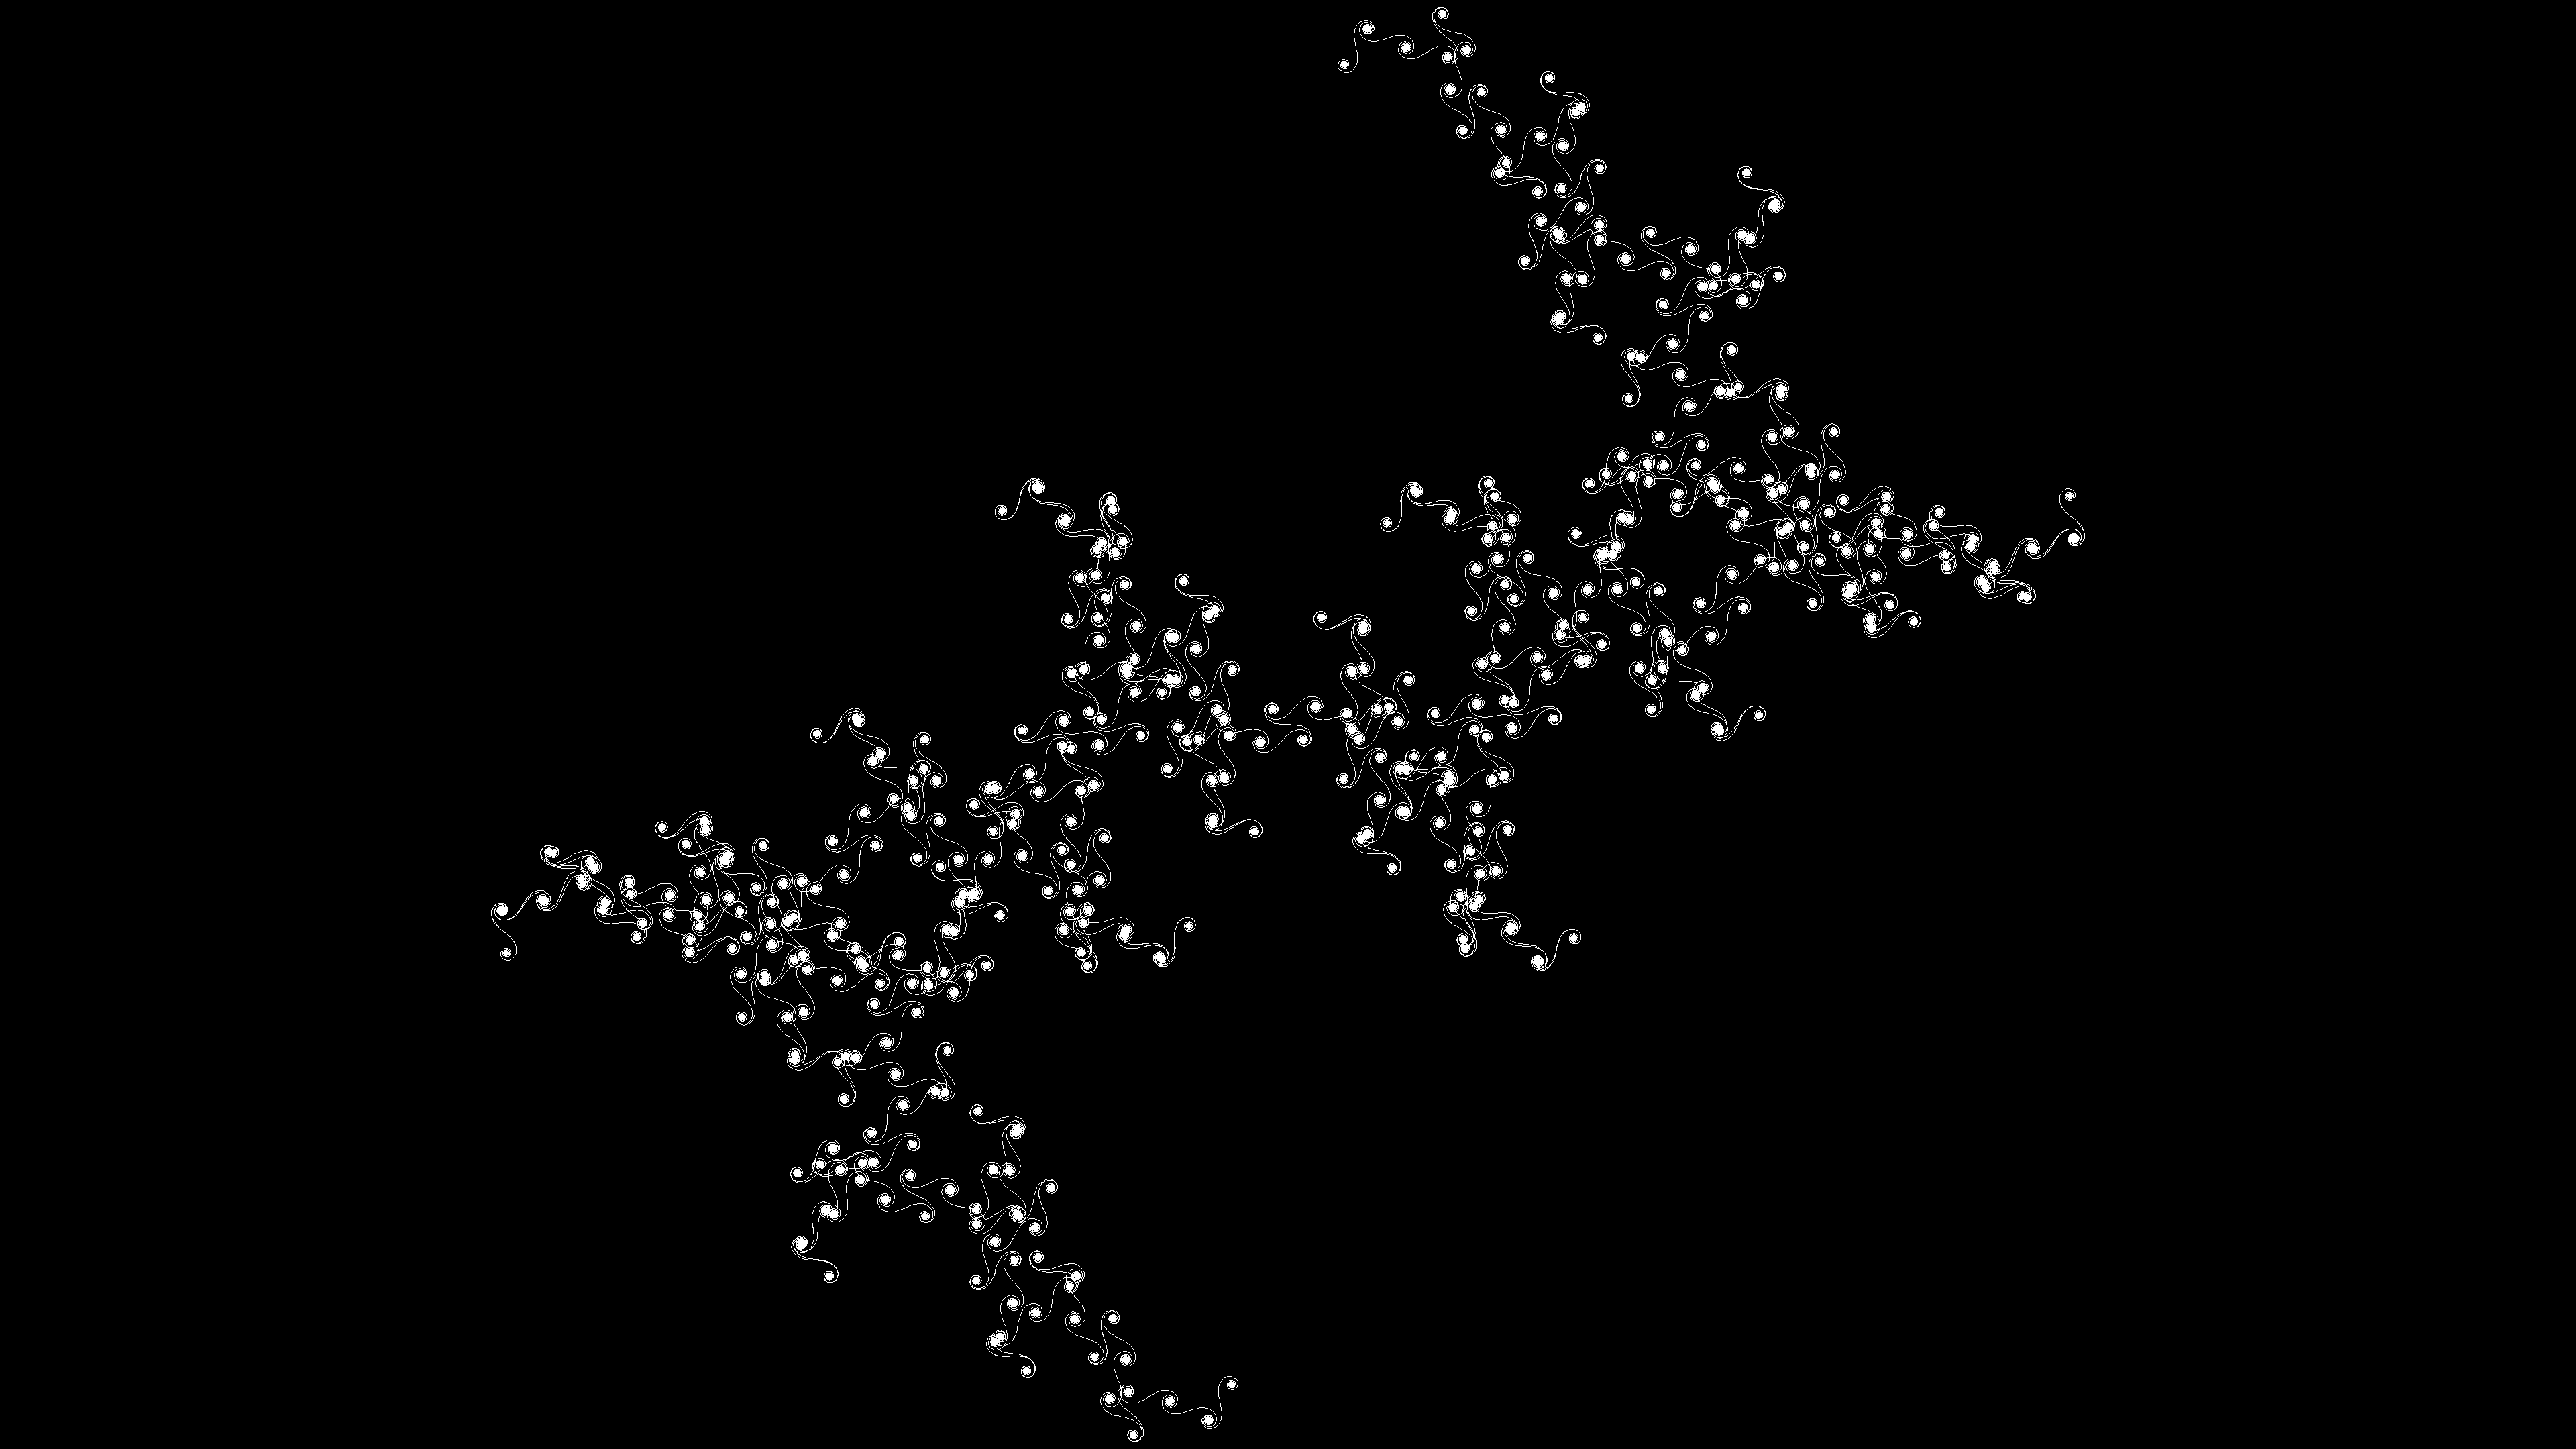
\includegraphics[width=\linewidth]{./stepsplusoneimages/0000000135.png}
    \caption{tf p=499 q=199734 theta=000 89939620.png}
  \end{subfigure}
  \begin{subfigure}[t]{0.48\textwidth}
    \centering
    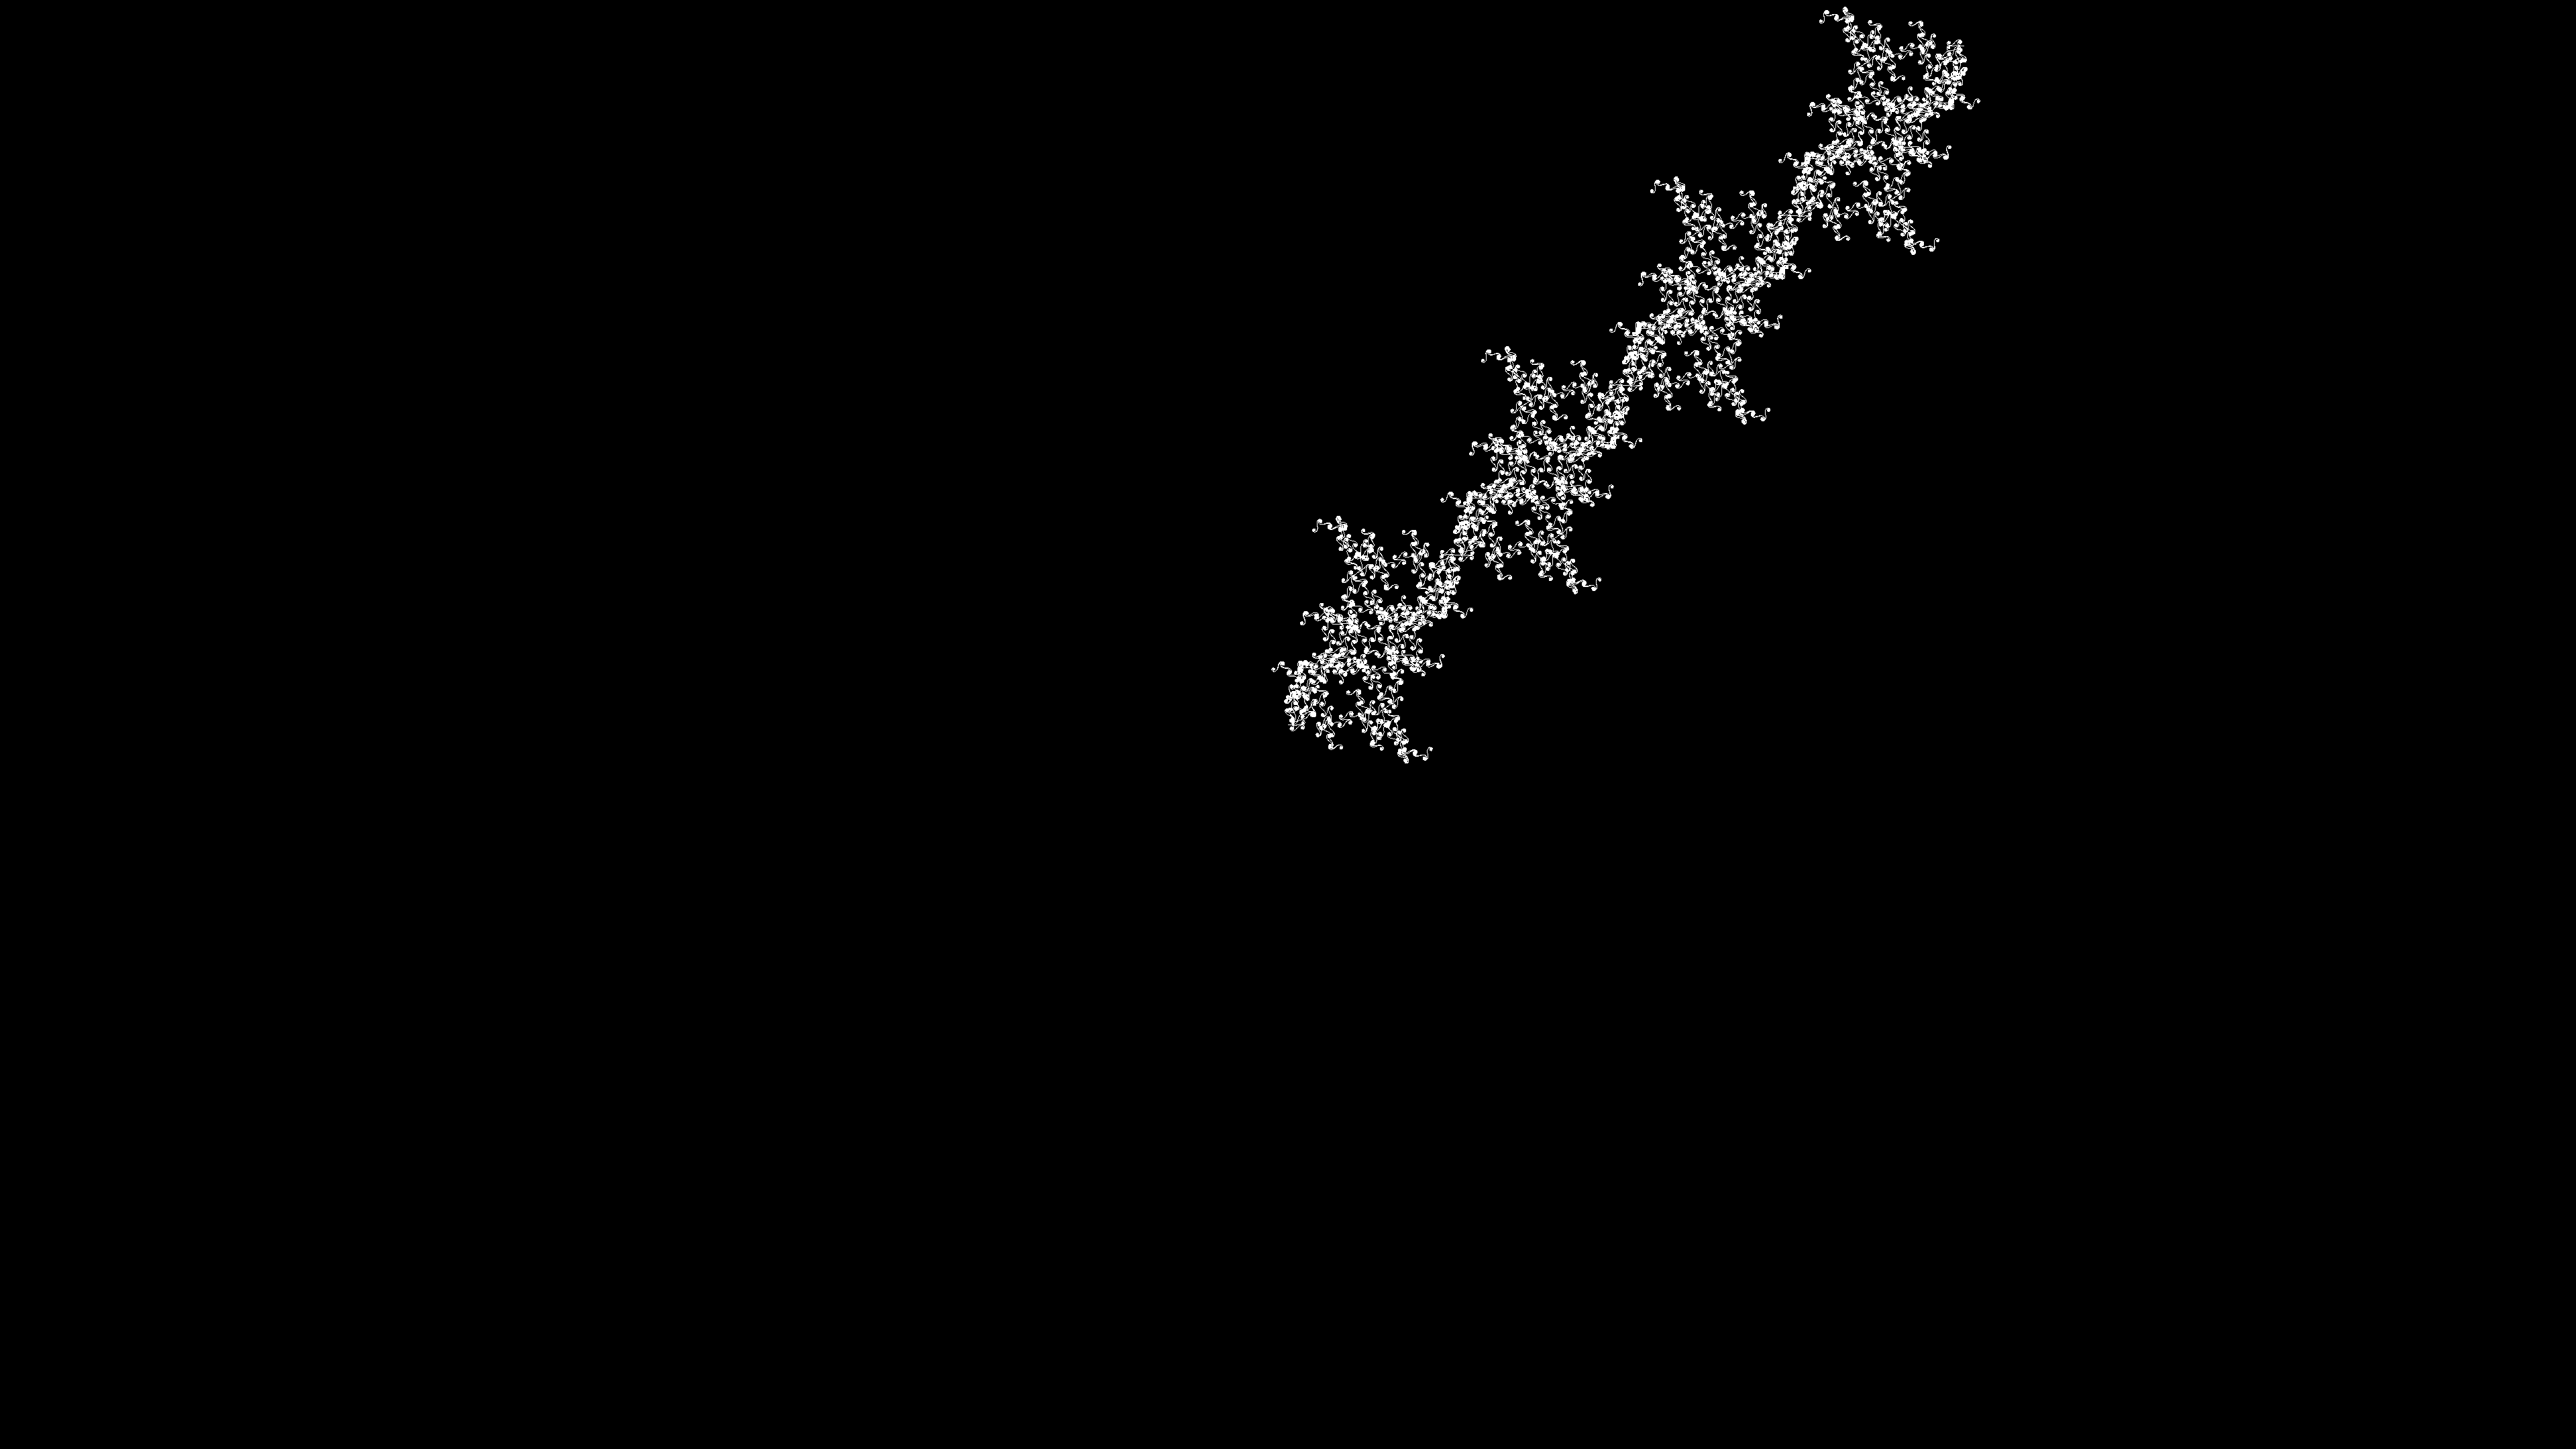
\includegraphics[width=\linewidth]{./stepsplusoneimages/0000000136.png}
    \caption{tf p=499 q=200233 theta=000 89715481.png}
  \end{subfigure}
  \caption{n=134 s=400 s+1=401}
  \label{fig:n=134}
\end{figure}
\begin{figure}[H]
  \centering
  \begin{subfigure}[t]{0.48\textwidth}
    \centering
    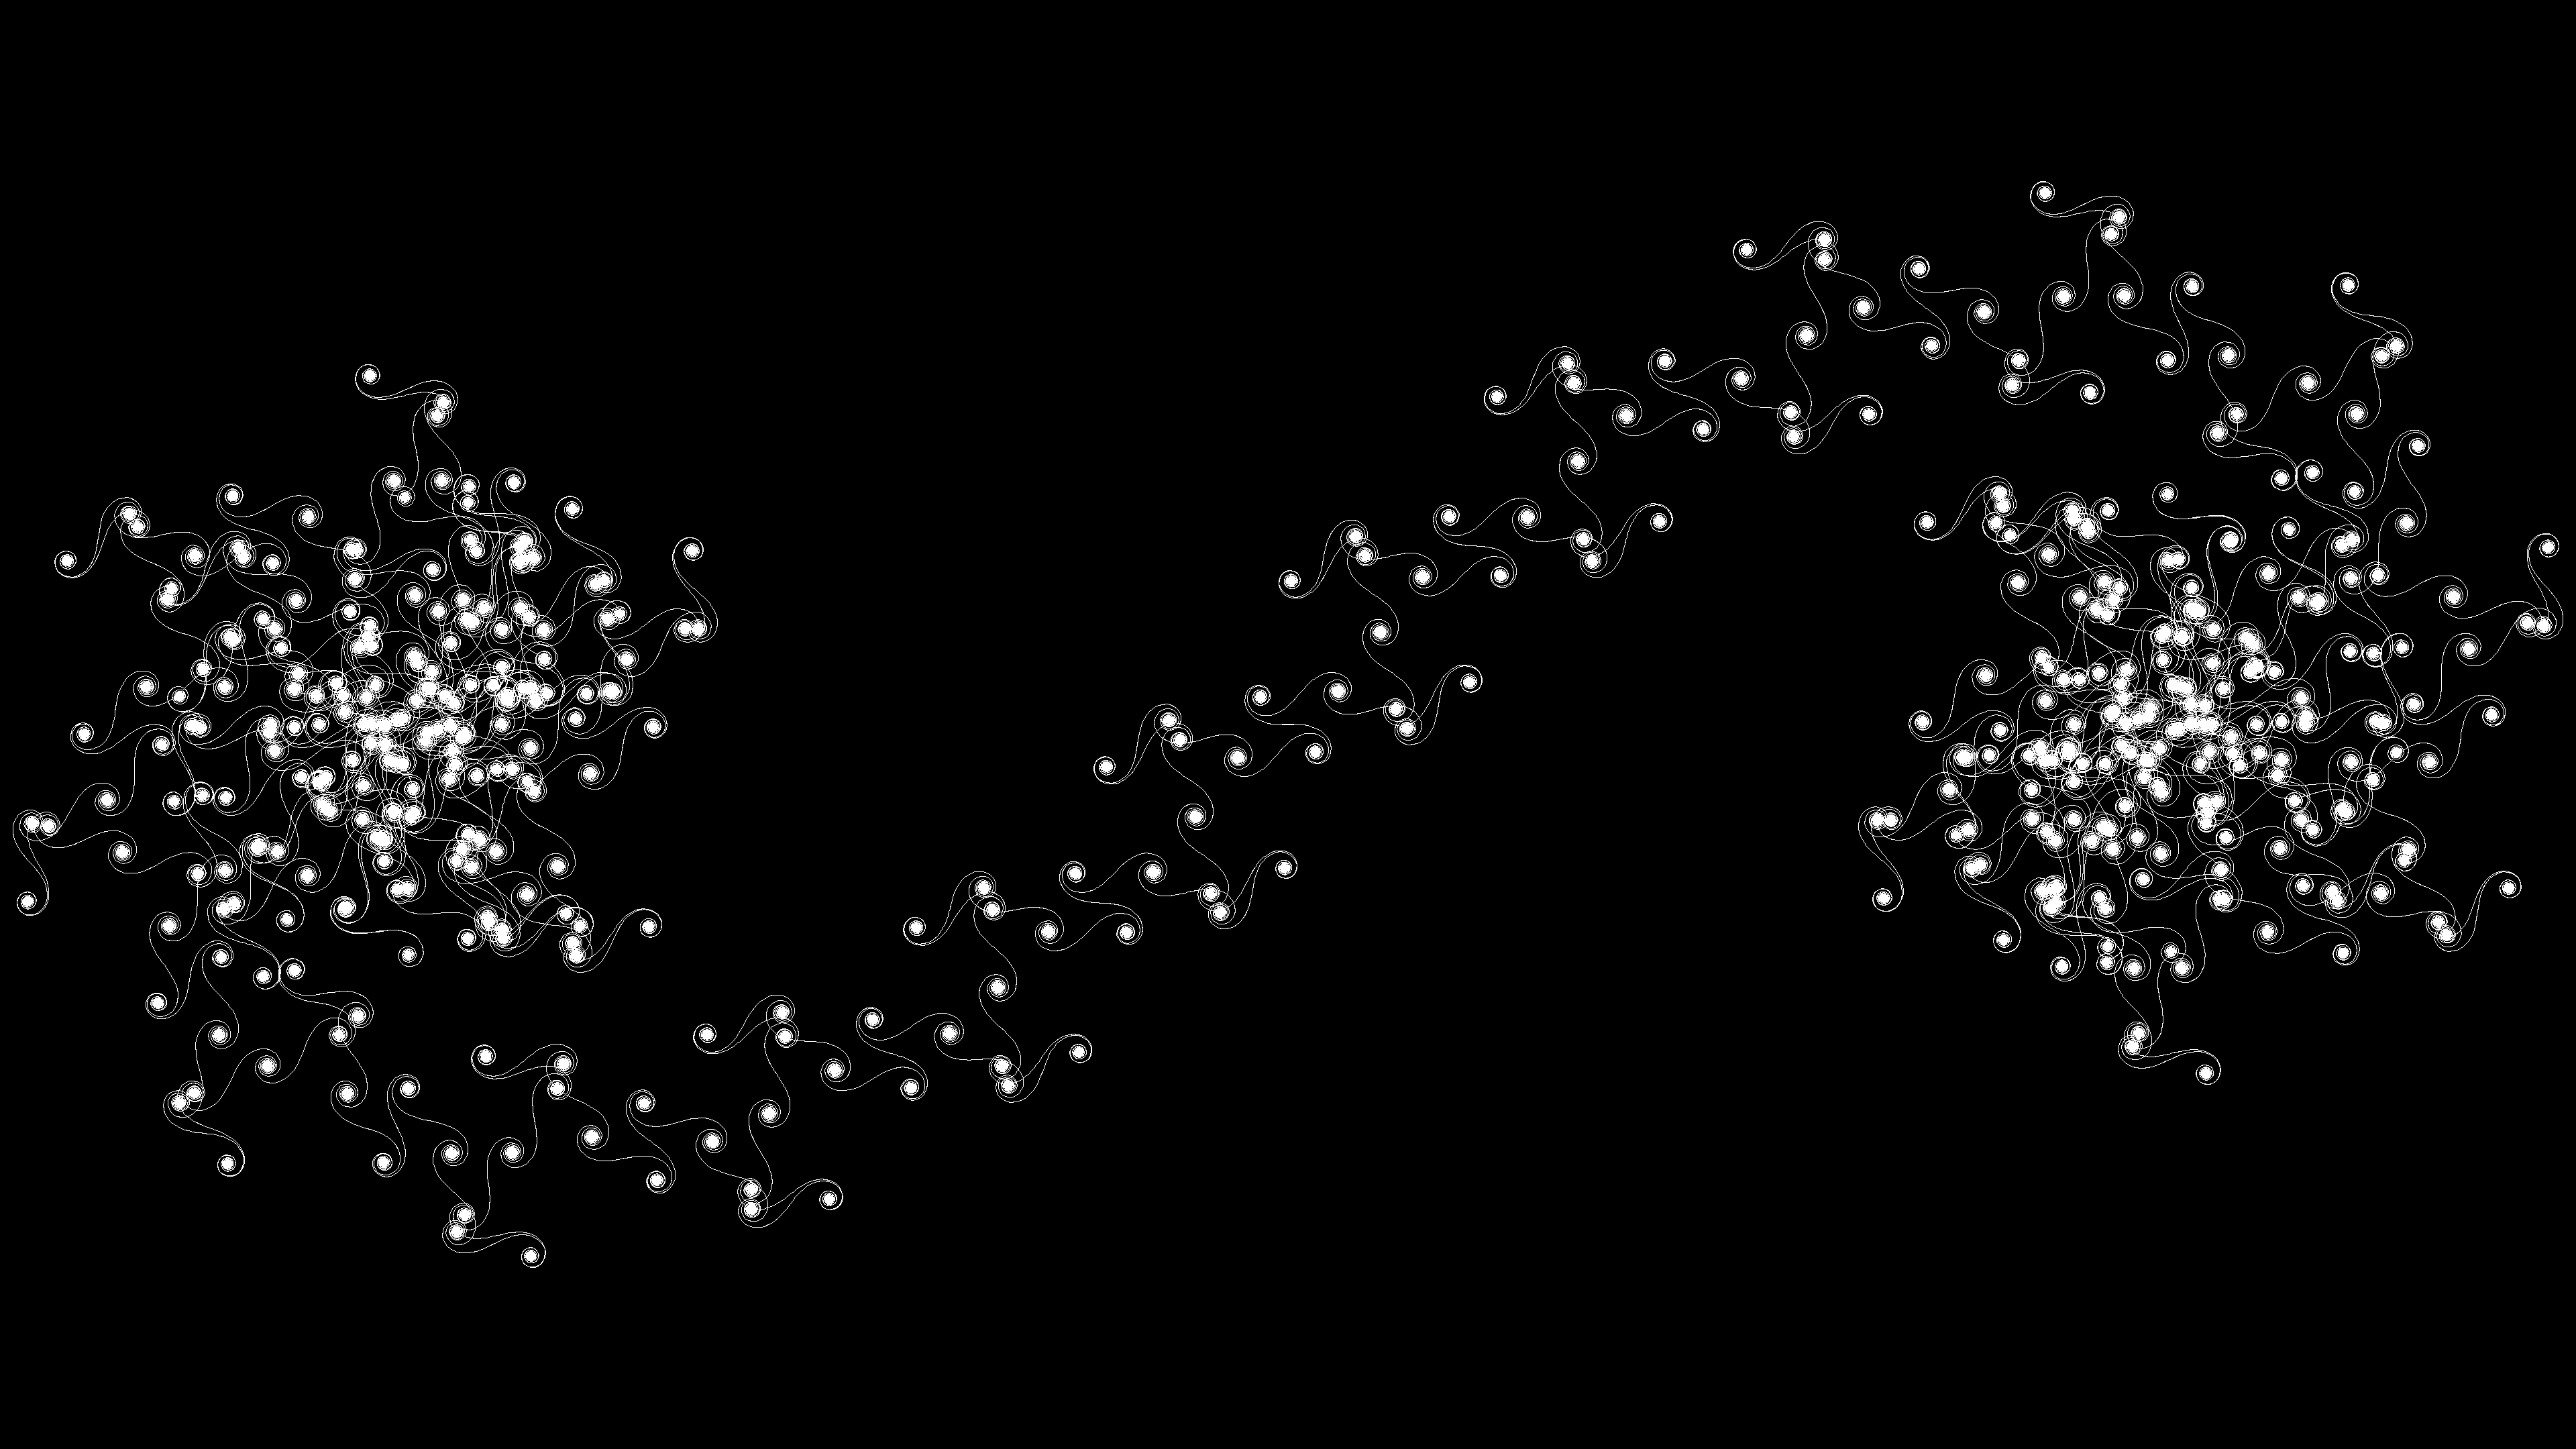
\includegraphics[width=\linewidth]{./stepsplusoneimages/0000000137.png}
    \caption{tf p=499 q=199736 theta=000 89938719.png}
  \end{subfigure}
  \begin{subfigure}[t]{0.48\textwidth}
    \centering
    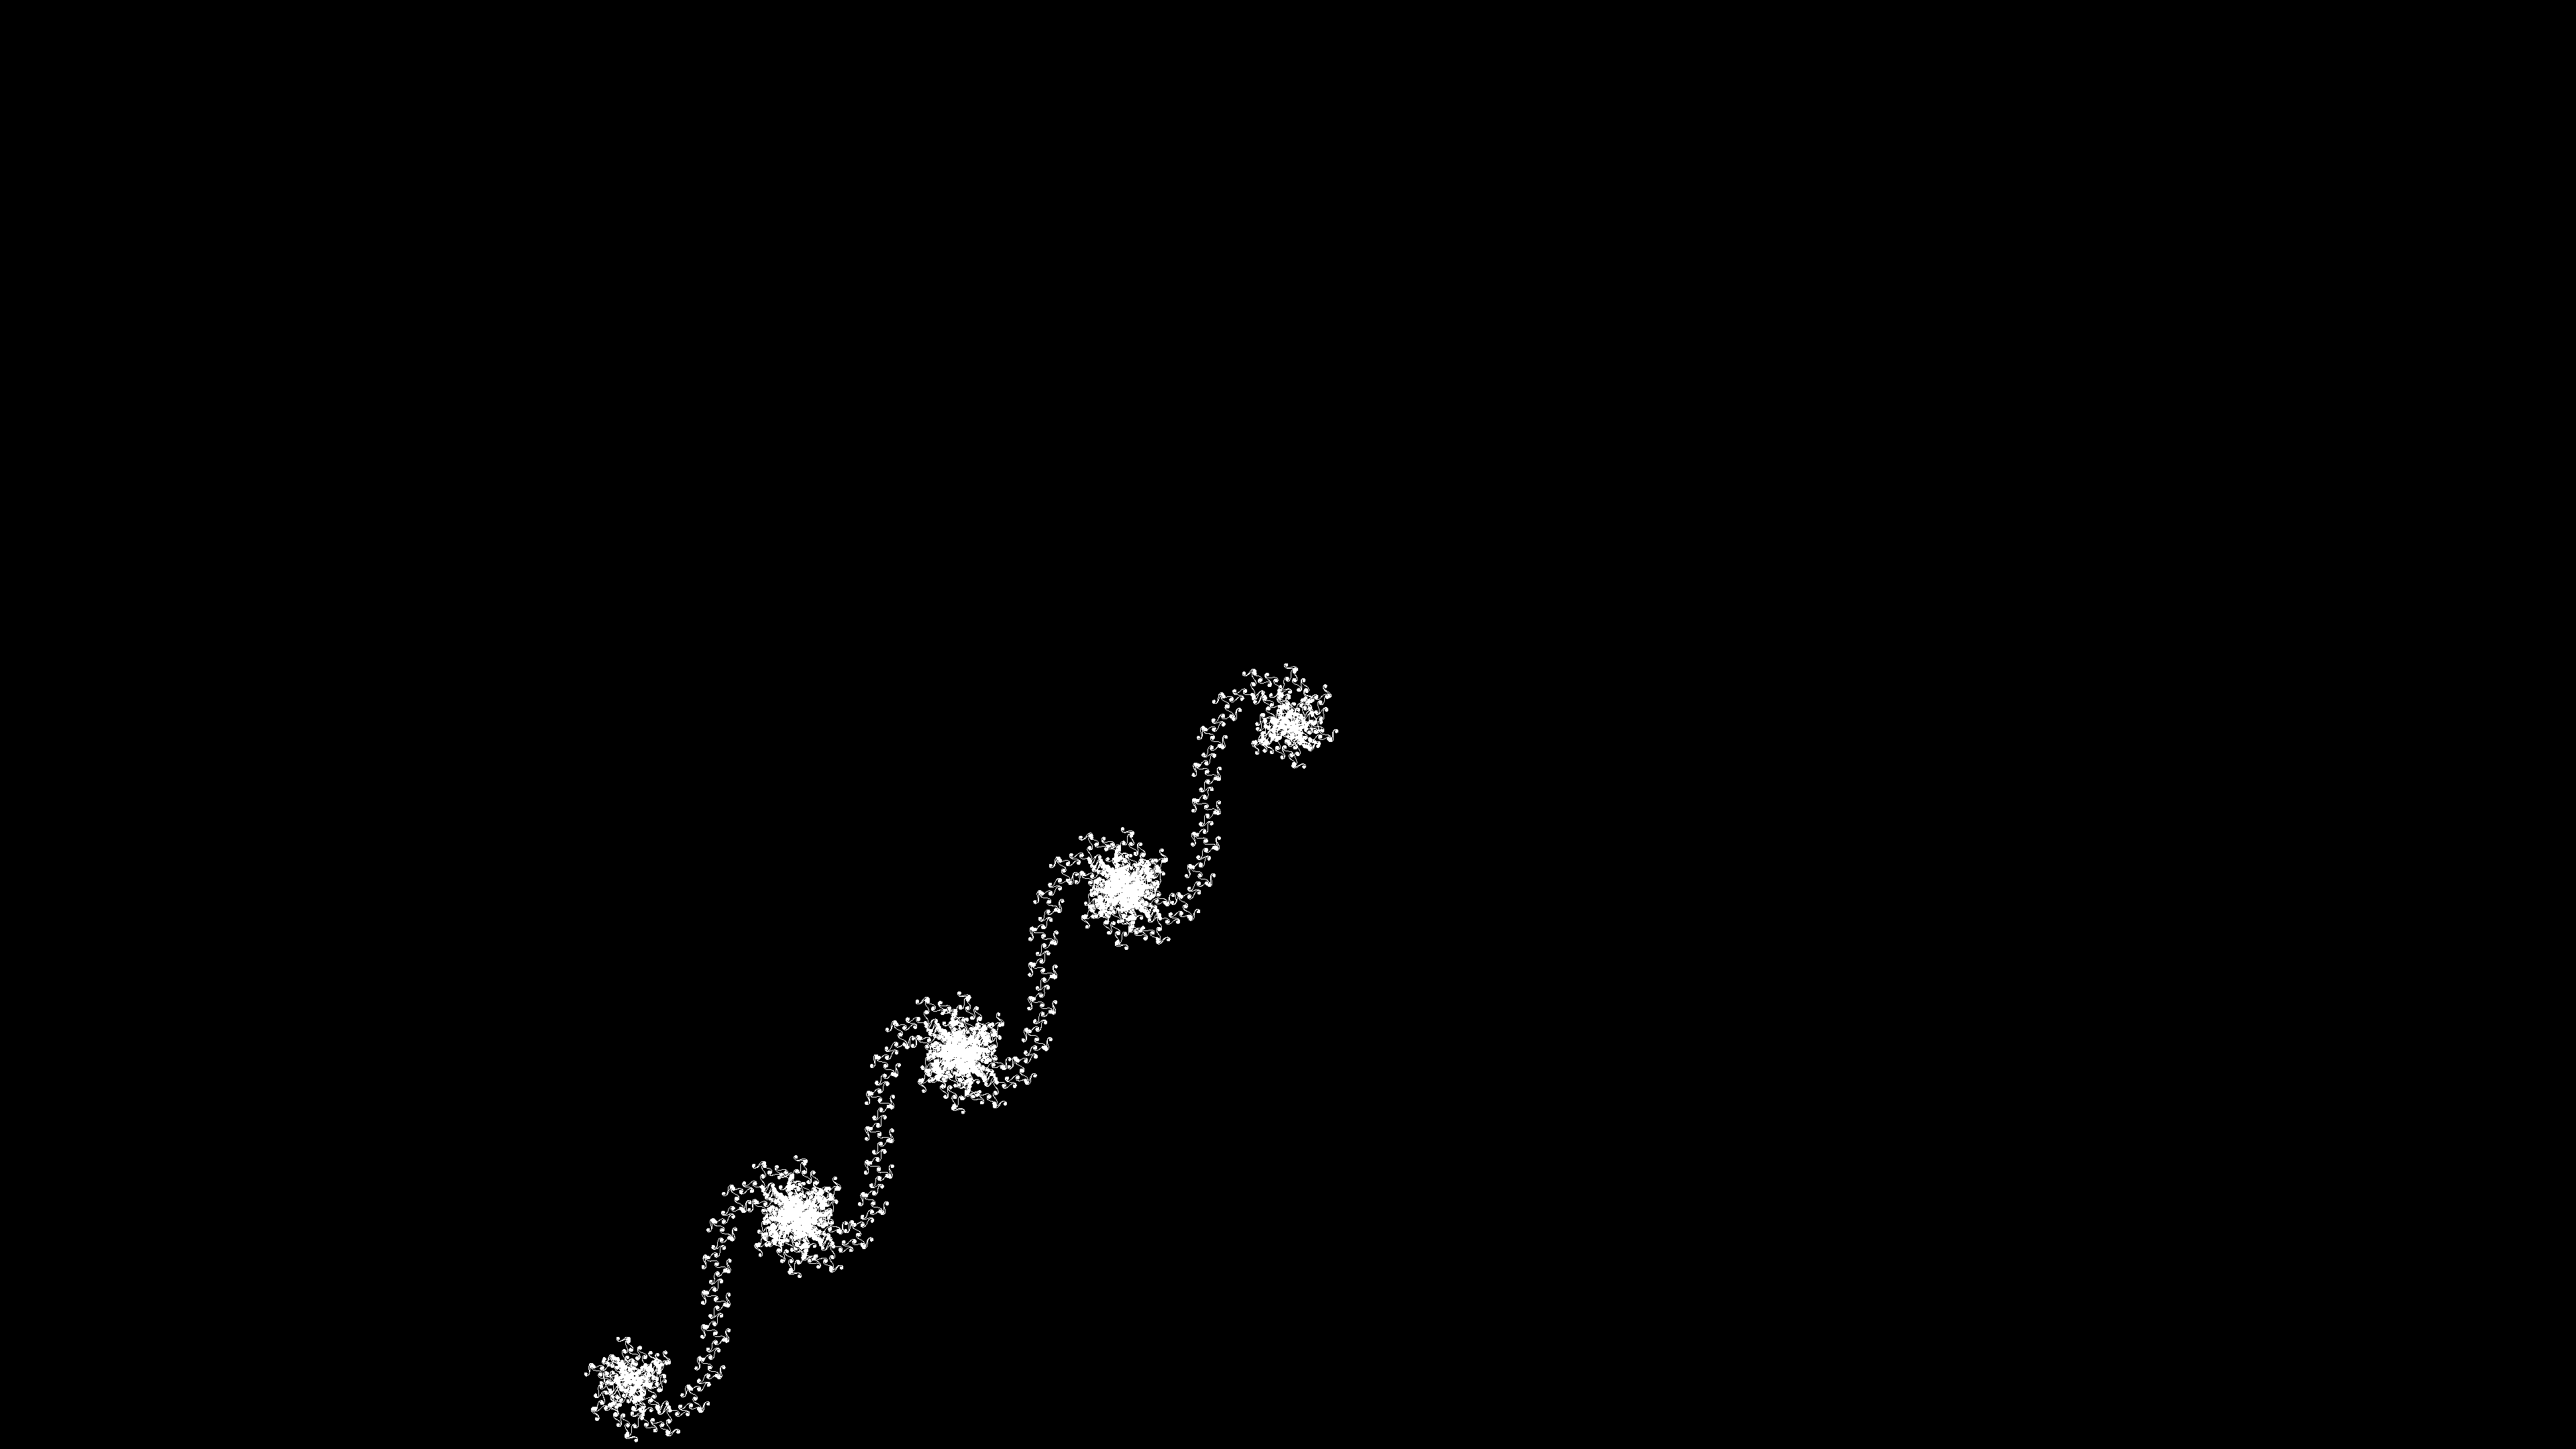
\includegraphics[width=\linewidth]{./stepsplusoneimages/0000000138.png}
    \caption{tf p=499 q=200235 theta=000 89714585.png}
  \end{subfigure}
  \caption{n=136 s=400 s+1=401}
  \label{fig:n=136}
\end{figure}
\begin{figure}[H]
  \centering
  \begin{subfigure}[t]{0.48\textwidth}
    \centering
    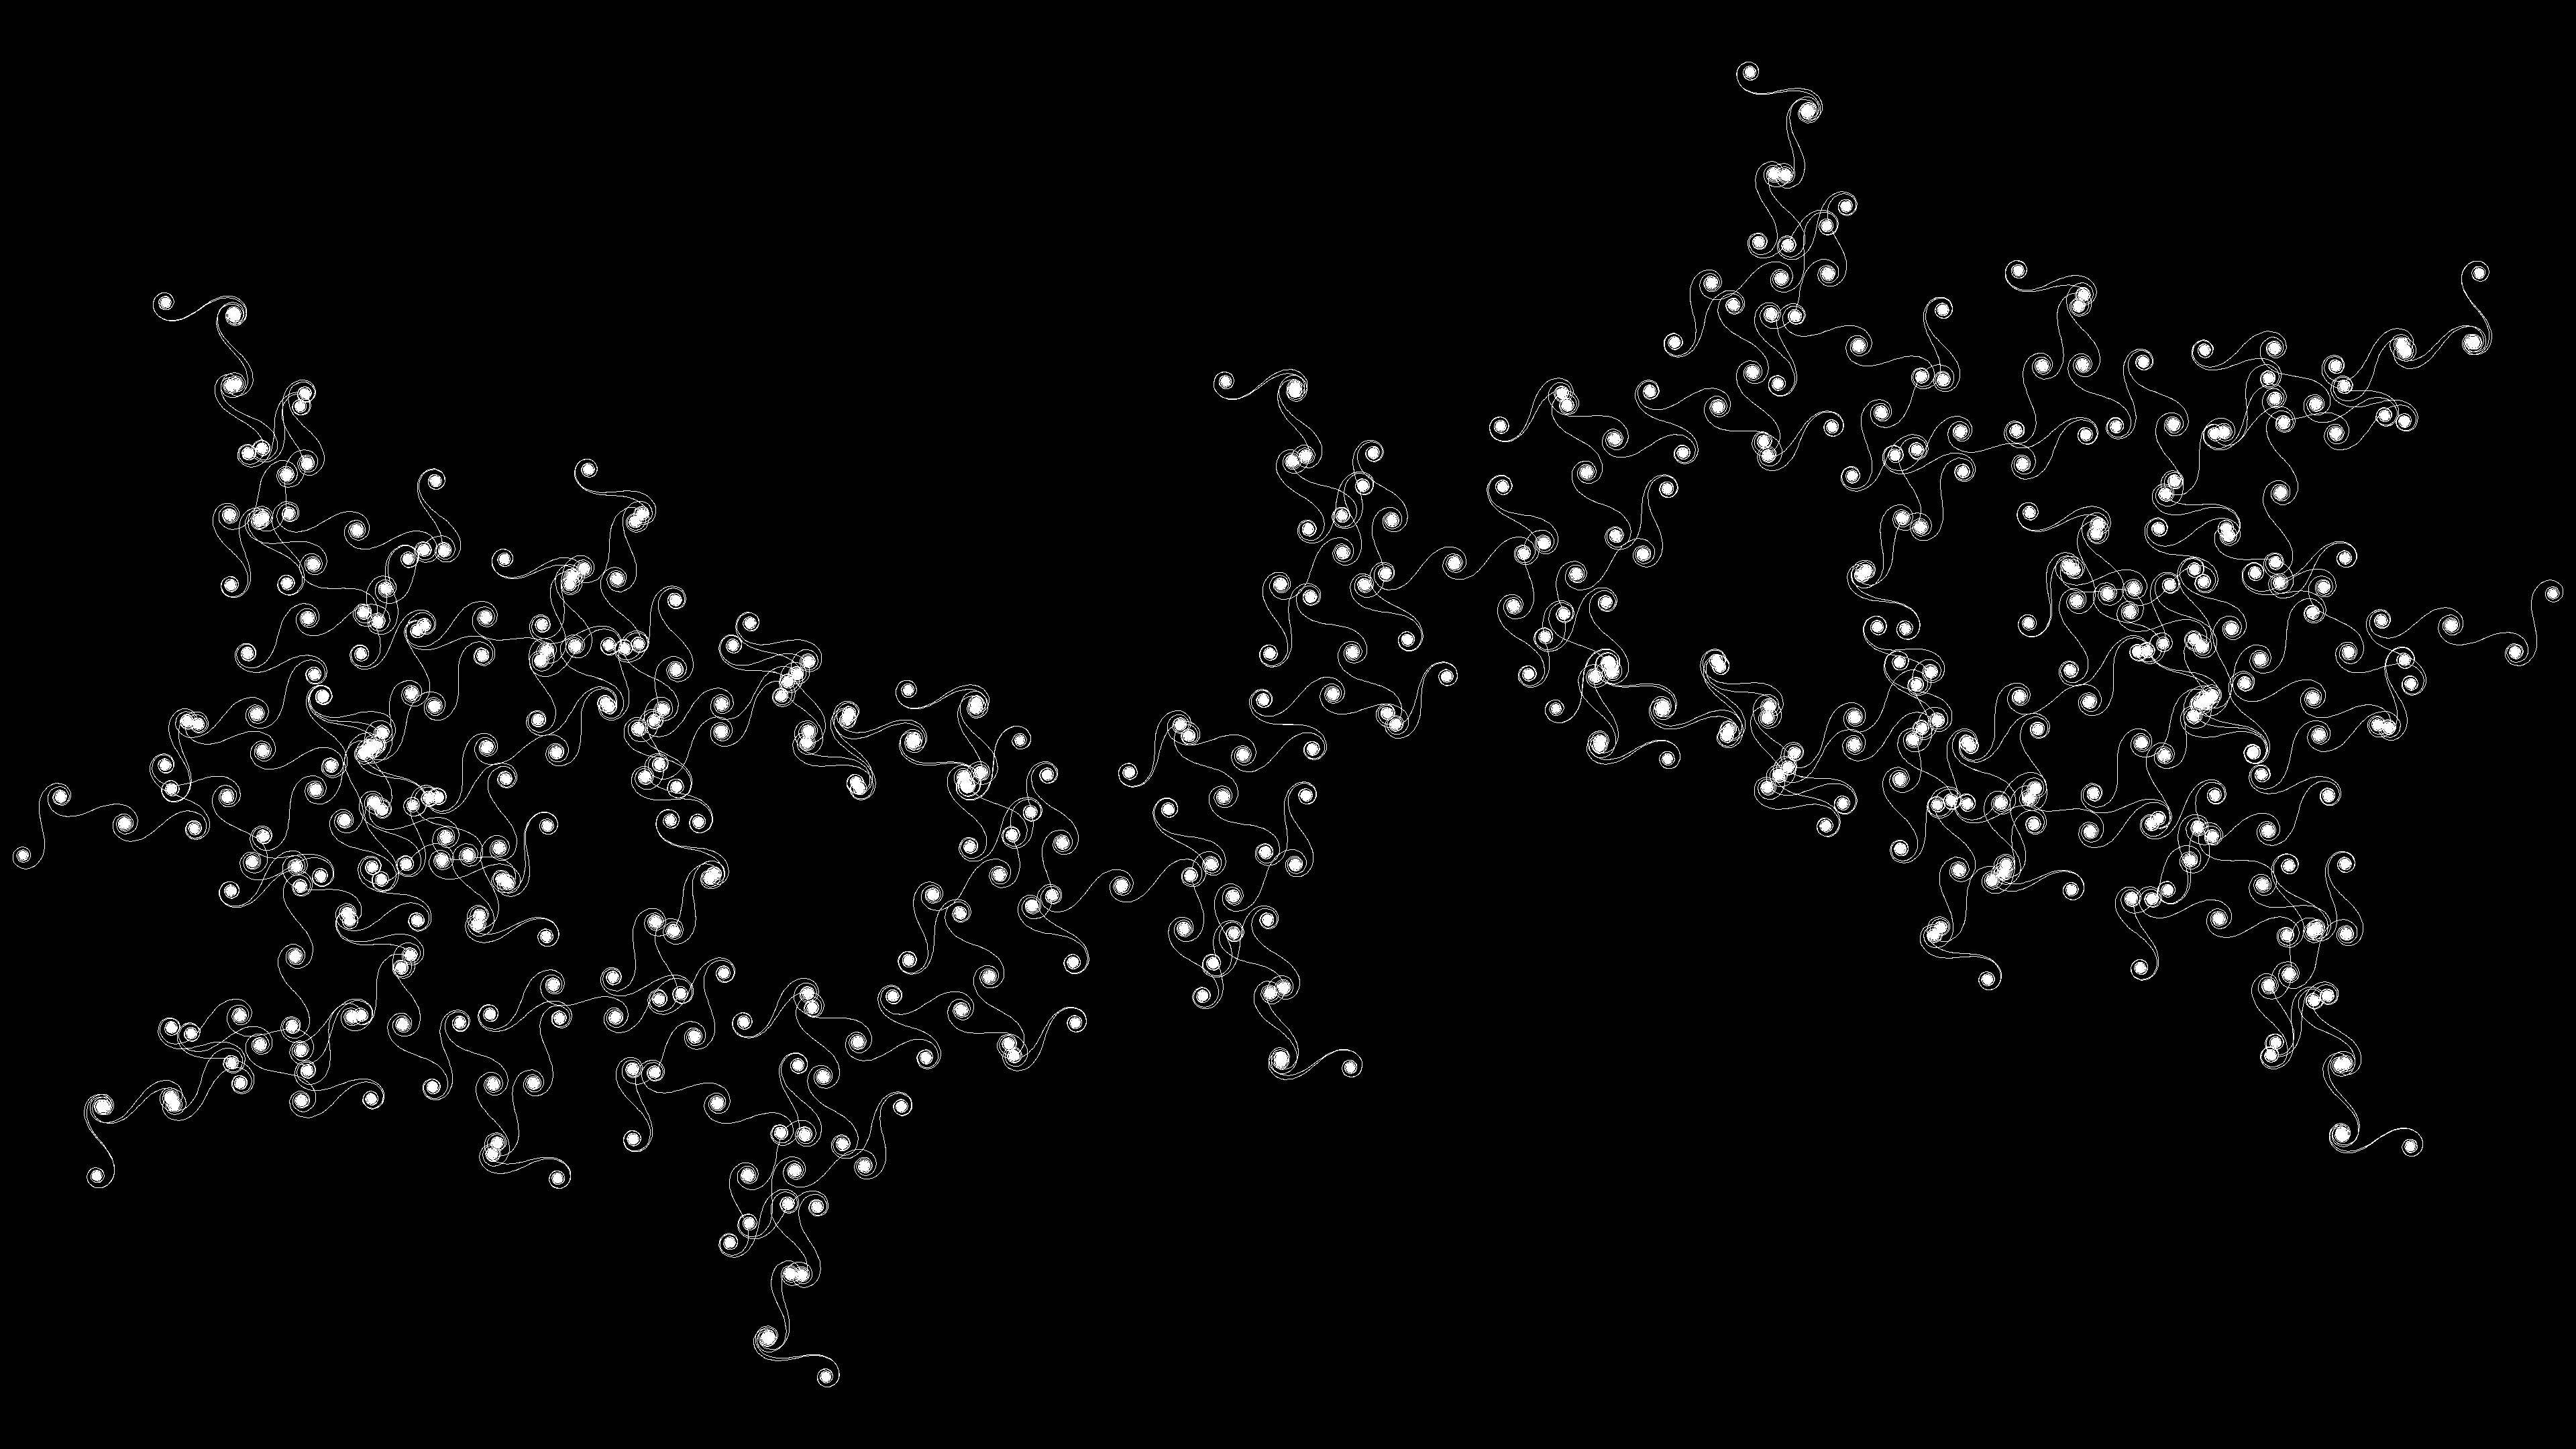
\includegraphics[width=\linewidth]{./stepsplusoneimages/0000000139.png}
    \caption{tf p=499 q=199738 theta=000 89937819.png}
  \end{subfigure}
  \begin{subfigure}[t]{0.48\textwidth}
    \centering
    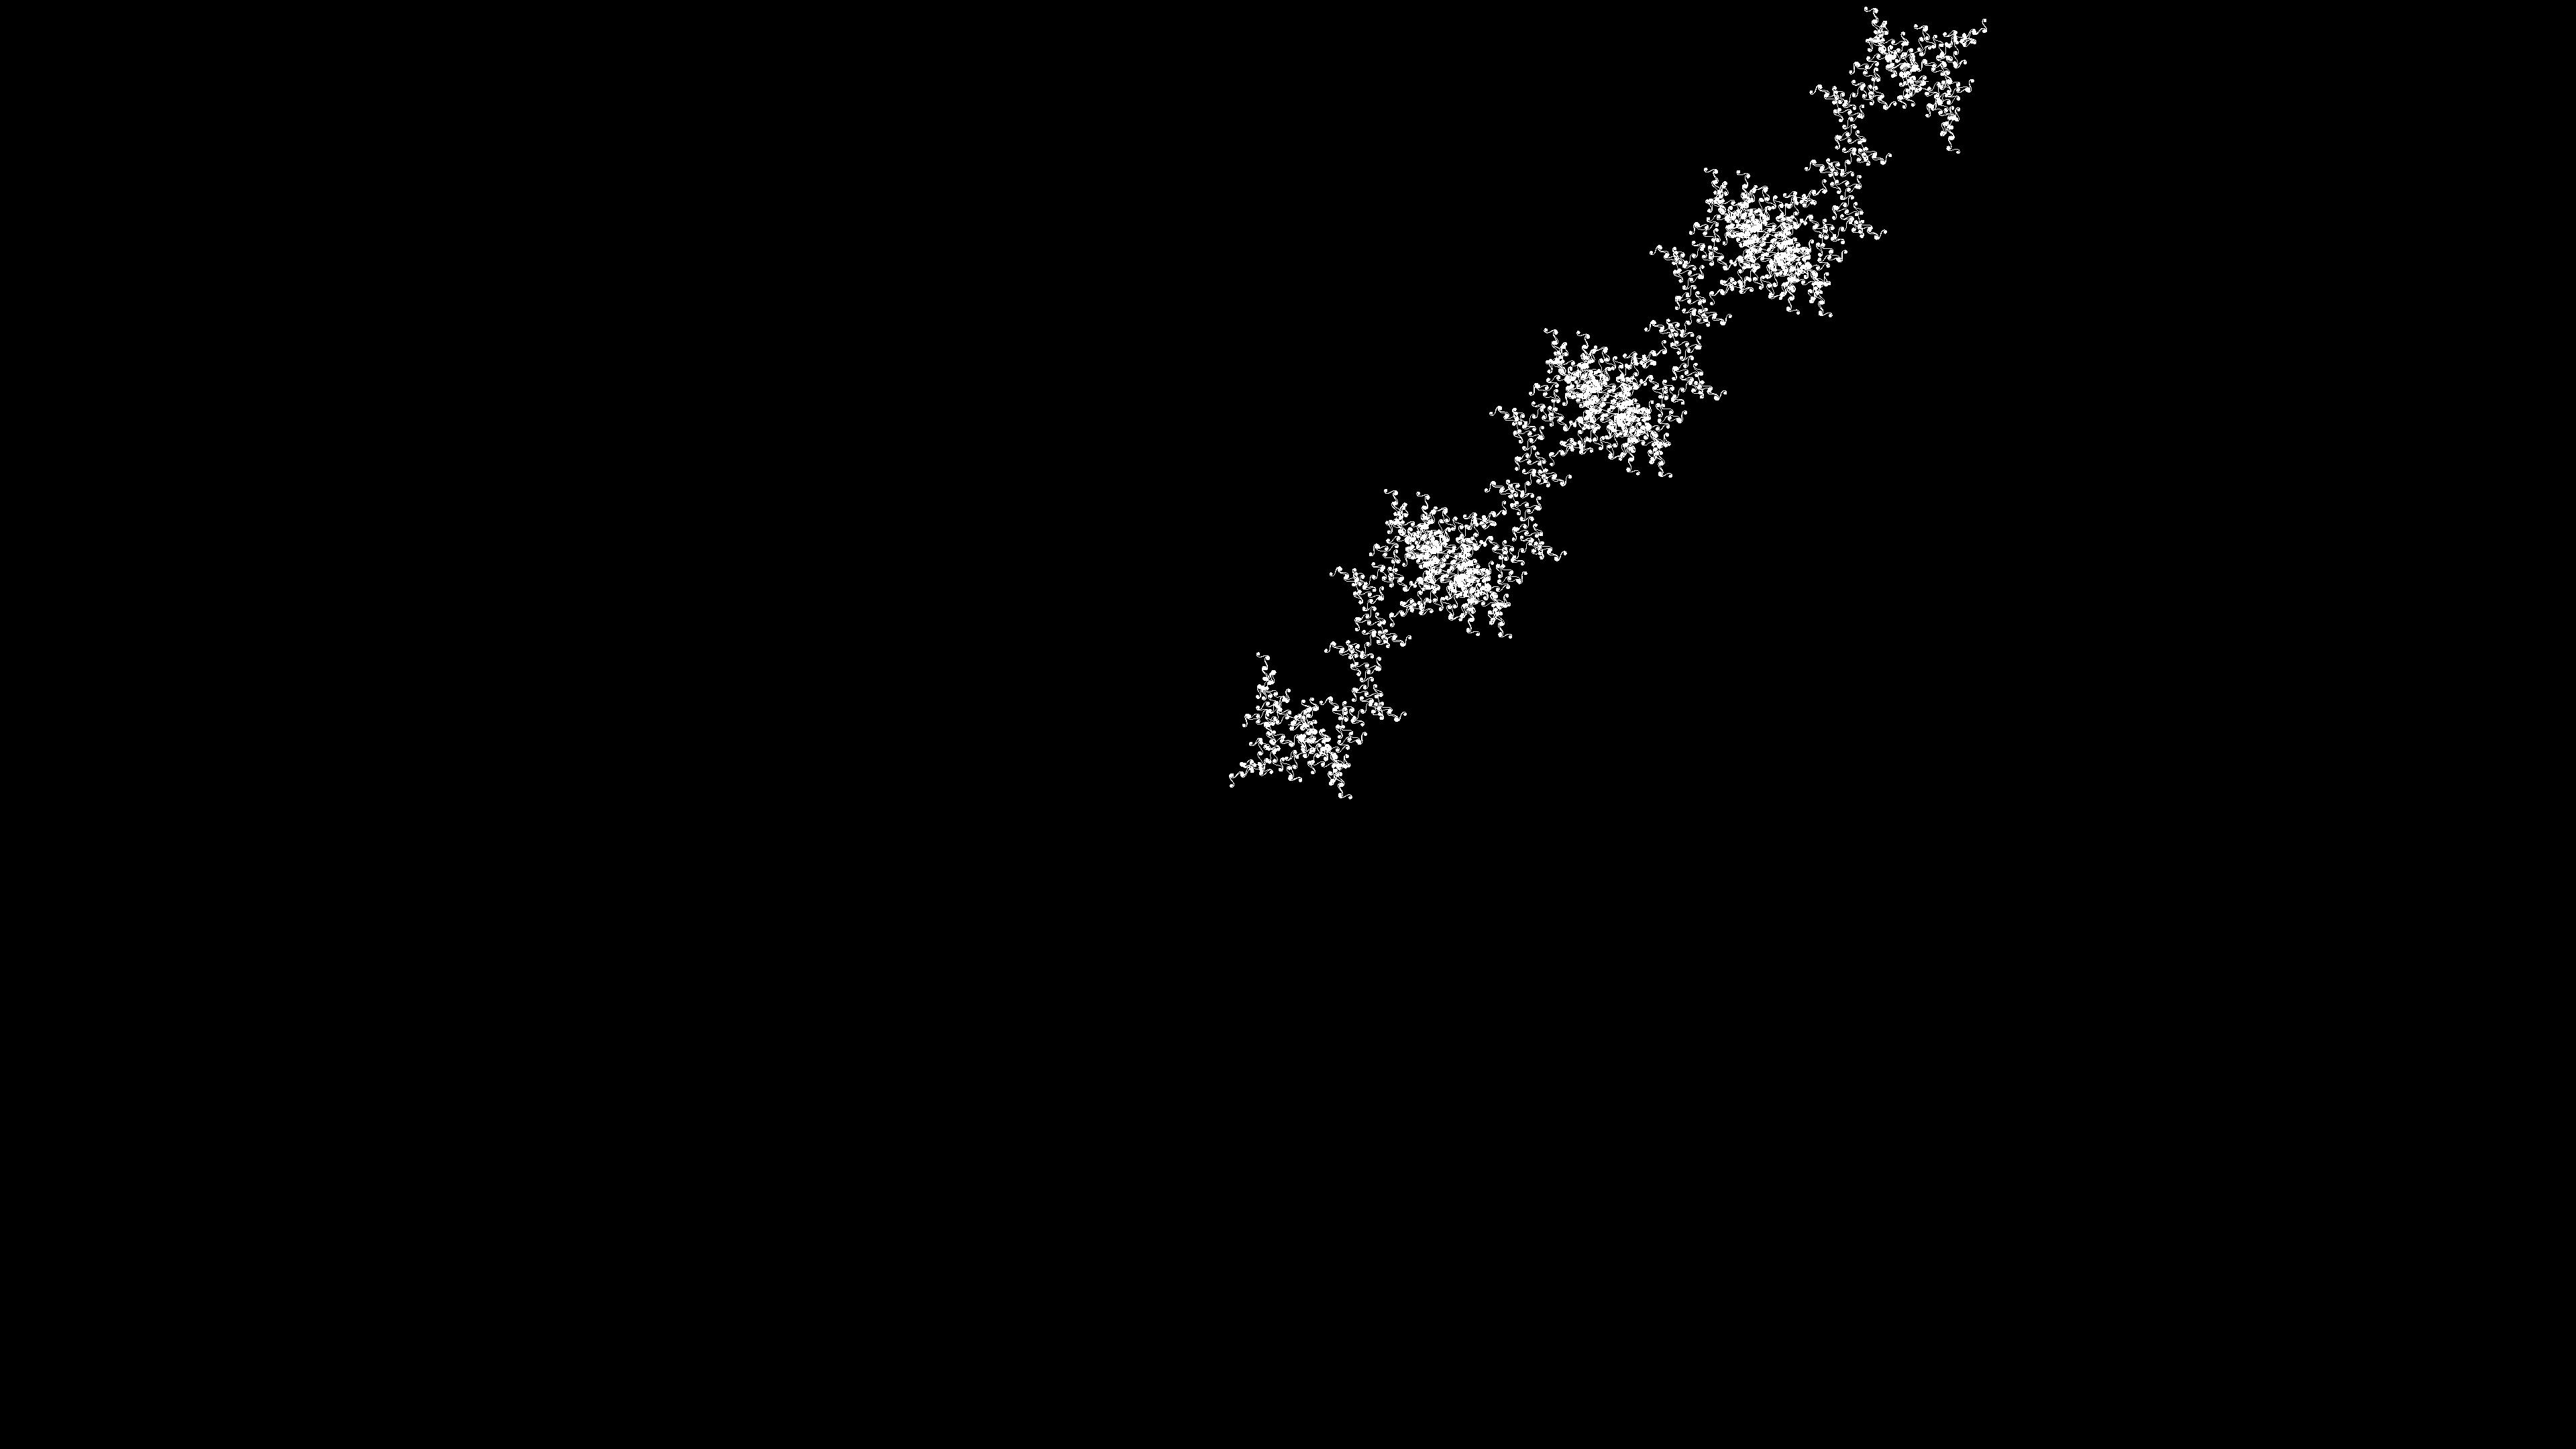
\includegraphics[width=\linewidth]{./stepsplusoneimages/0000000140.png}
    \caption{tf p=499 q=200237 theta=000 89713689.png}
  \end{subfigure}
  \caption{n=138 s=400 s+1=401}
  \label{fig:n=138}
\end{figure}
\begin{figure}[H]
  \centering
  \begin{subfigure}[t]{0.48\textwidth}
    \centering
    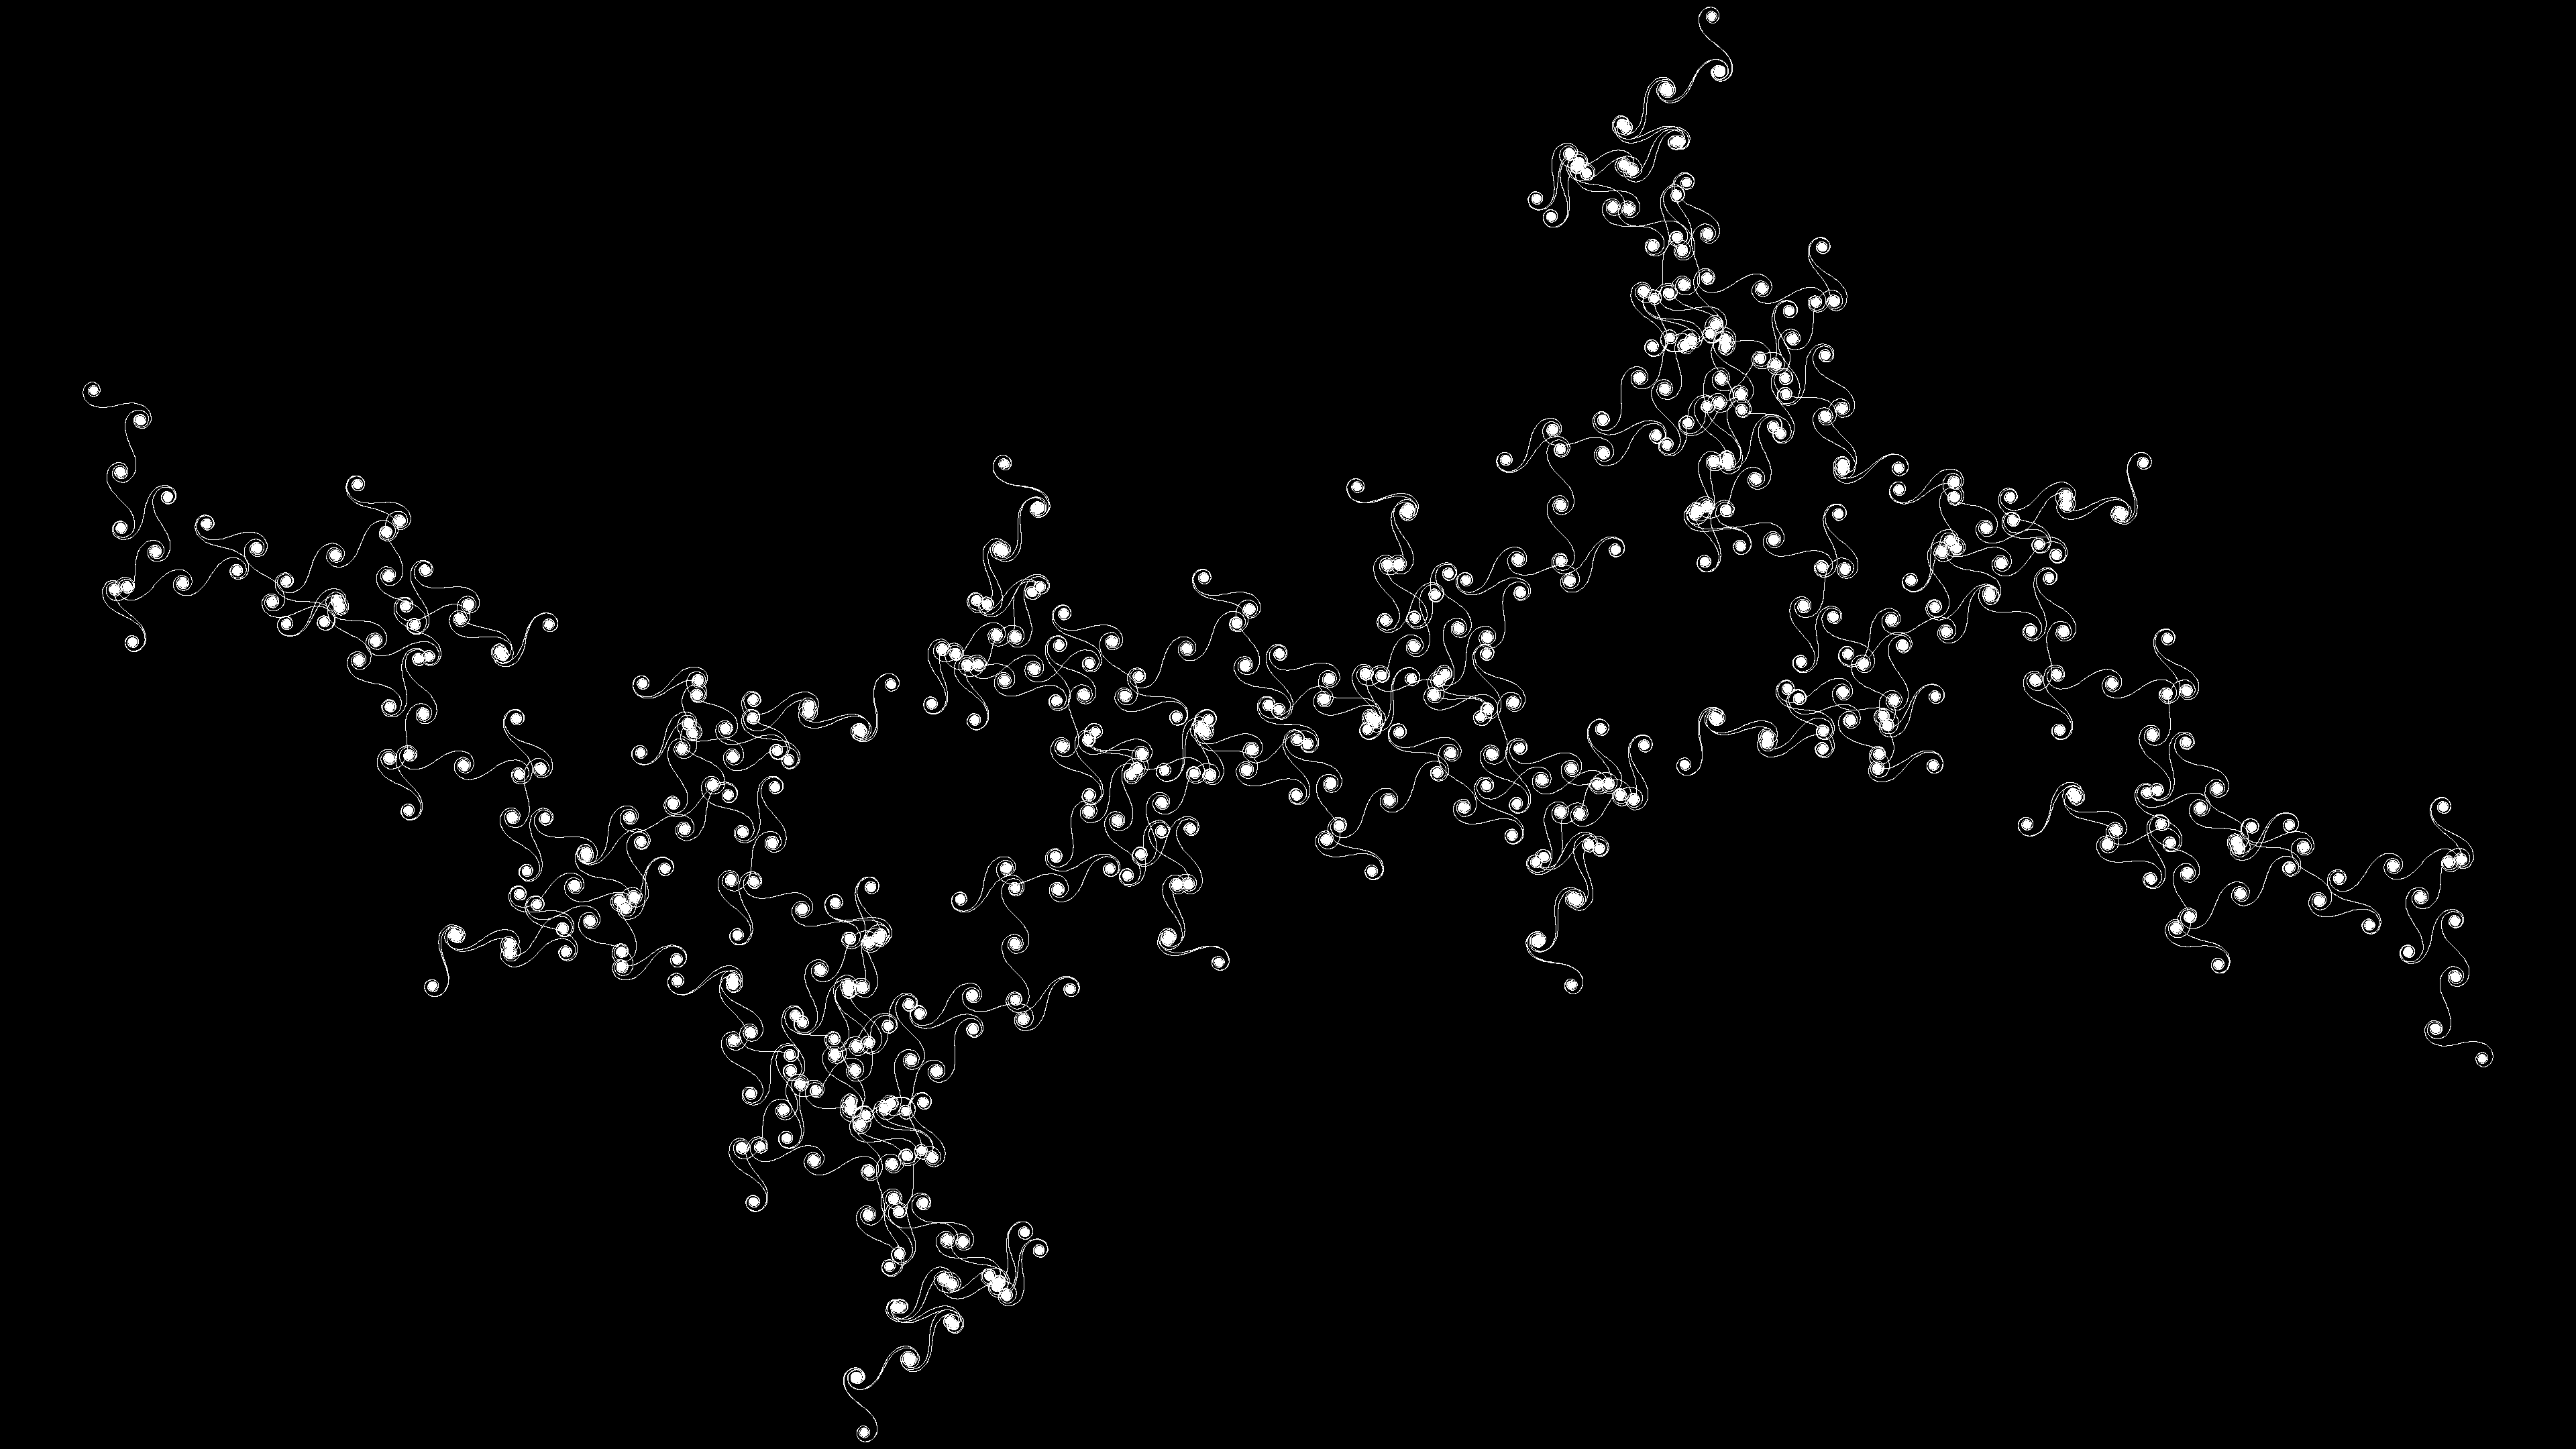
\includegraphics[width=\linewidth]{./stepsplusoneimages/0000000141.png}
    \caption{tf p=499 q=199740 theta=000 89936918.png}
  \end{subfigure}
  \begin{subfigure}[t]{0.48\textwidth}
    \centering
    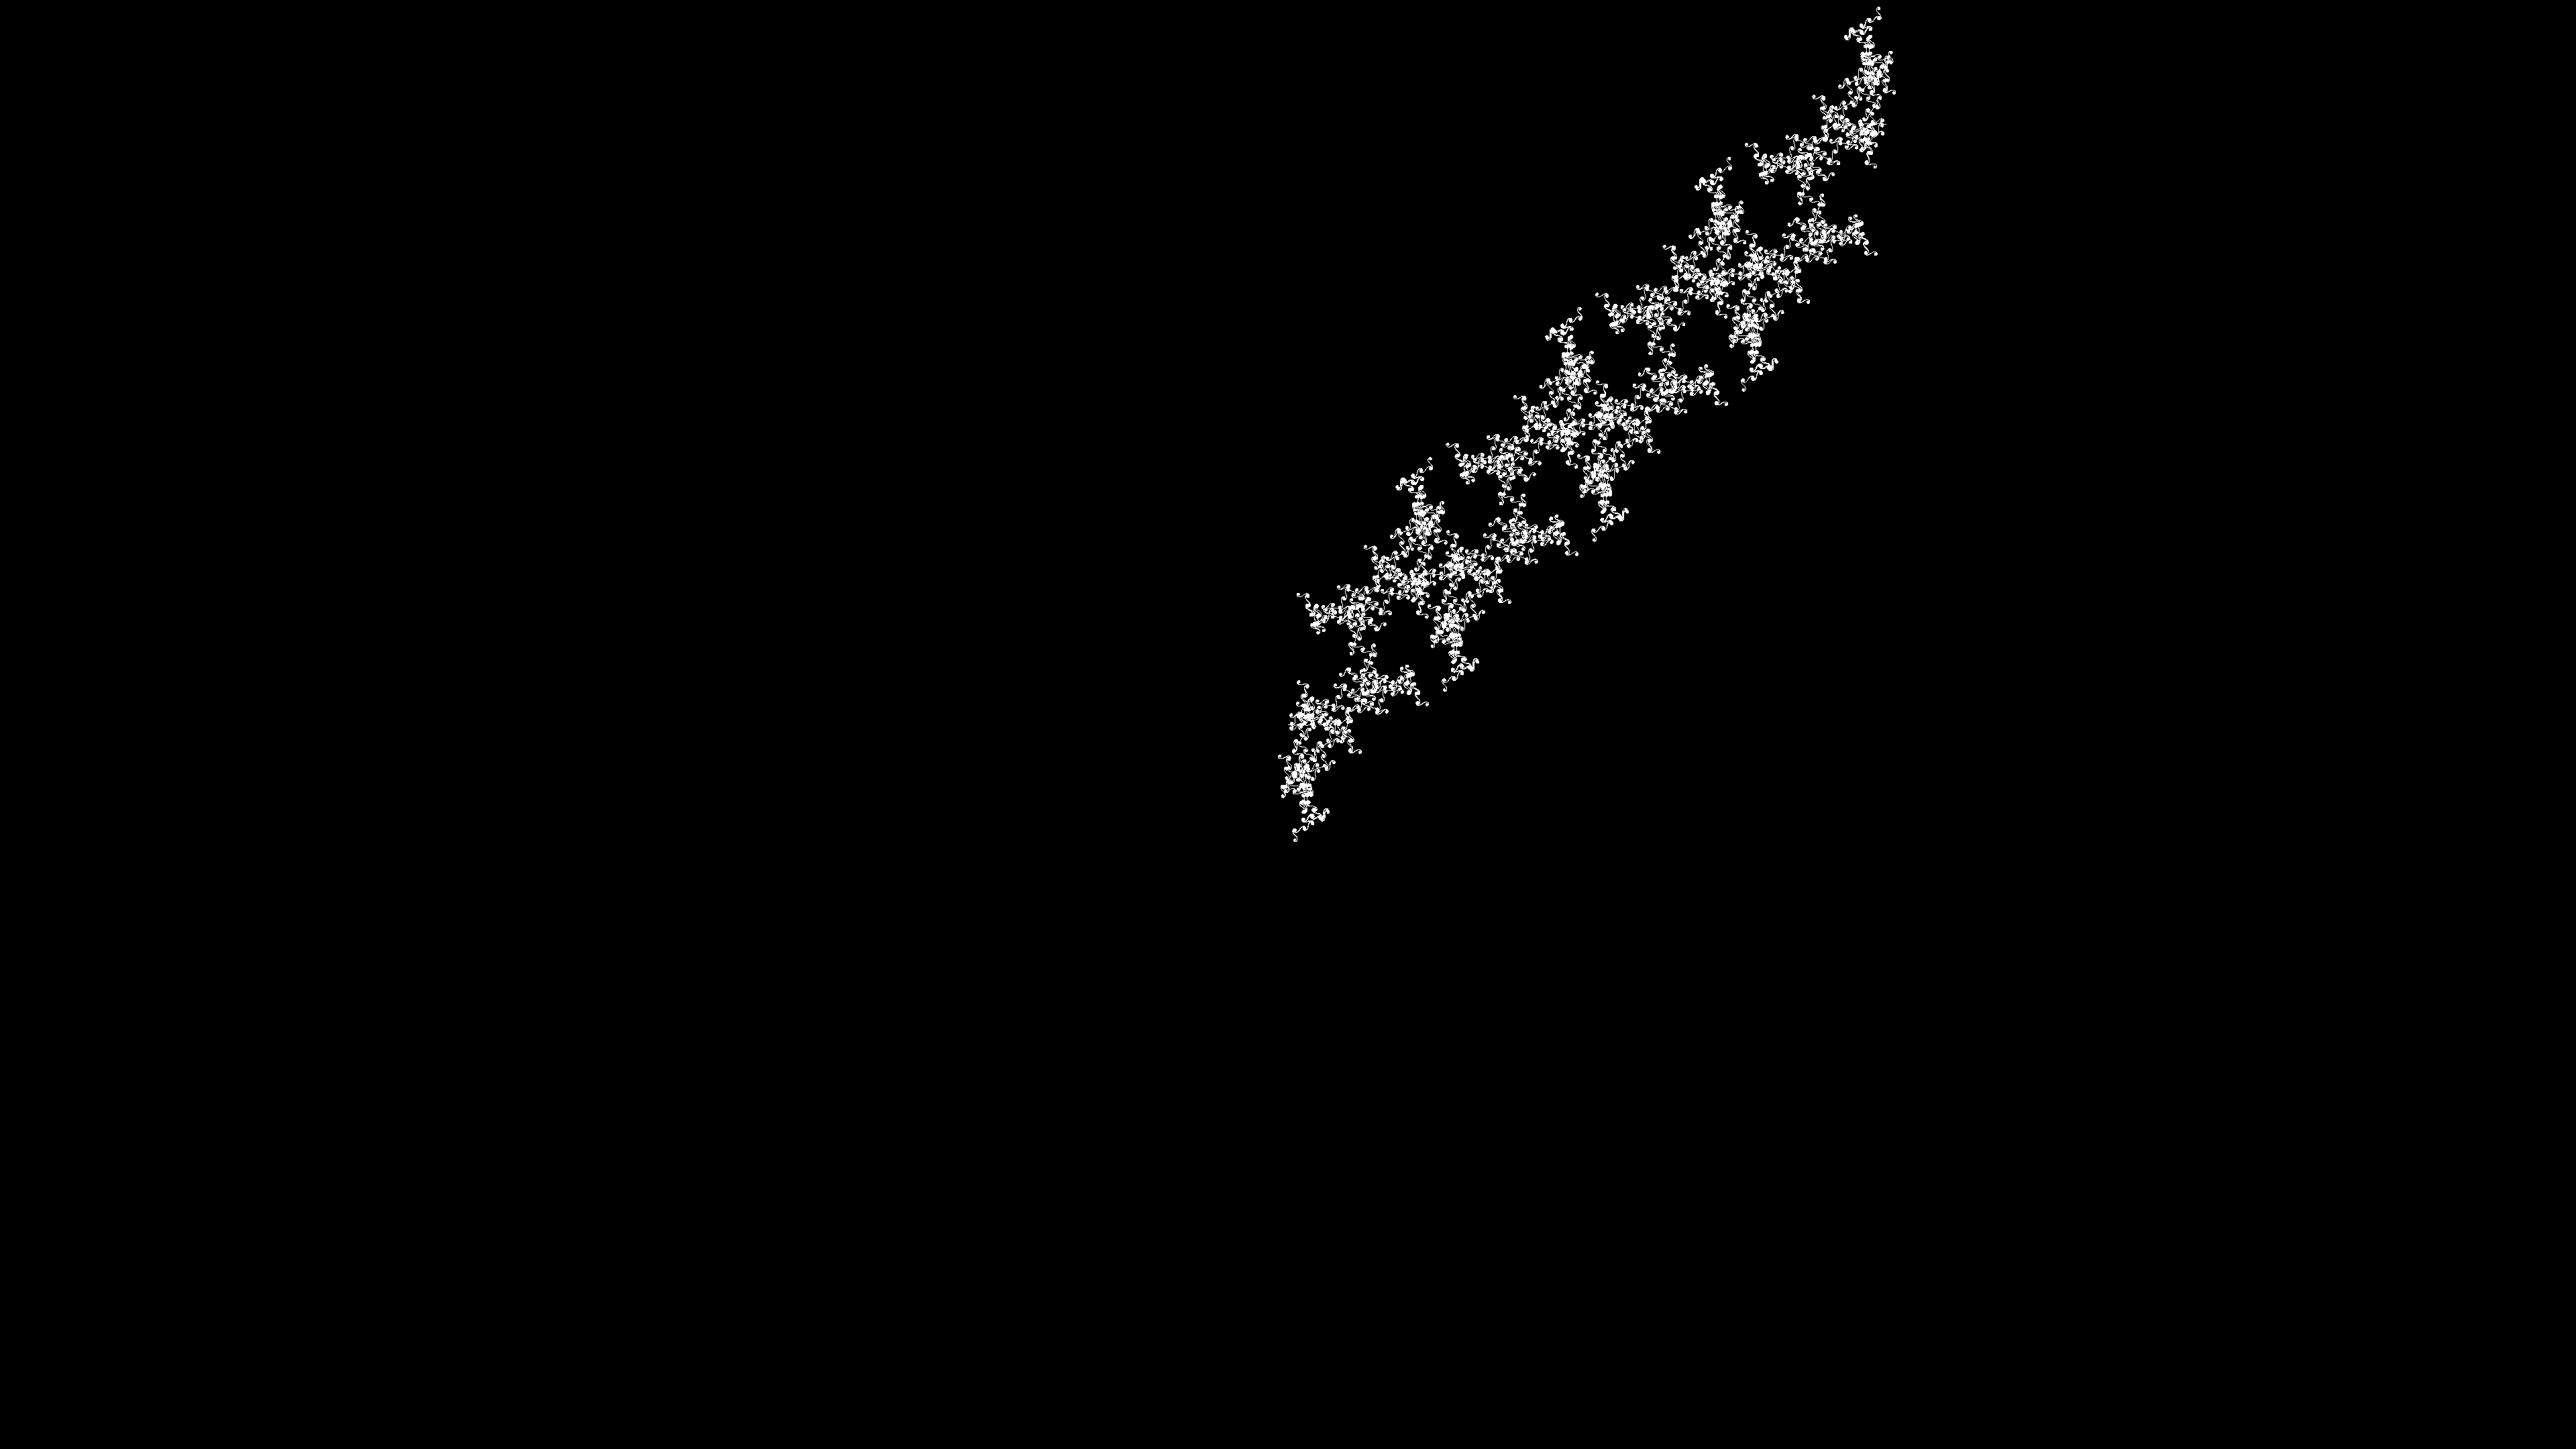
\includegraphics[width=\linewidth]{./stepsplusoneimages/0000000142.png}
    \caption{tf p=499 q=200239 theta=000 89712793.png}
  \end{subfigure}
  \caption{n=140 s=400 s+1=401}
  \label{fig:n=140}
\end{figure}
\begin{figure}[H]
  \centering
  \begin{subfigure}[t]{0.48\textwidth}
    \centering
    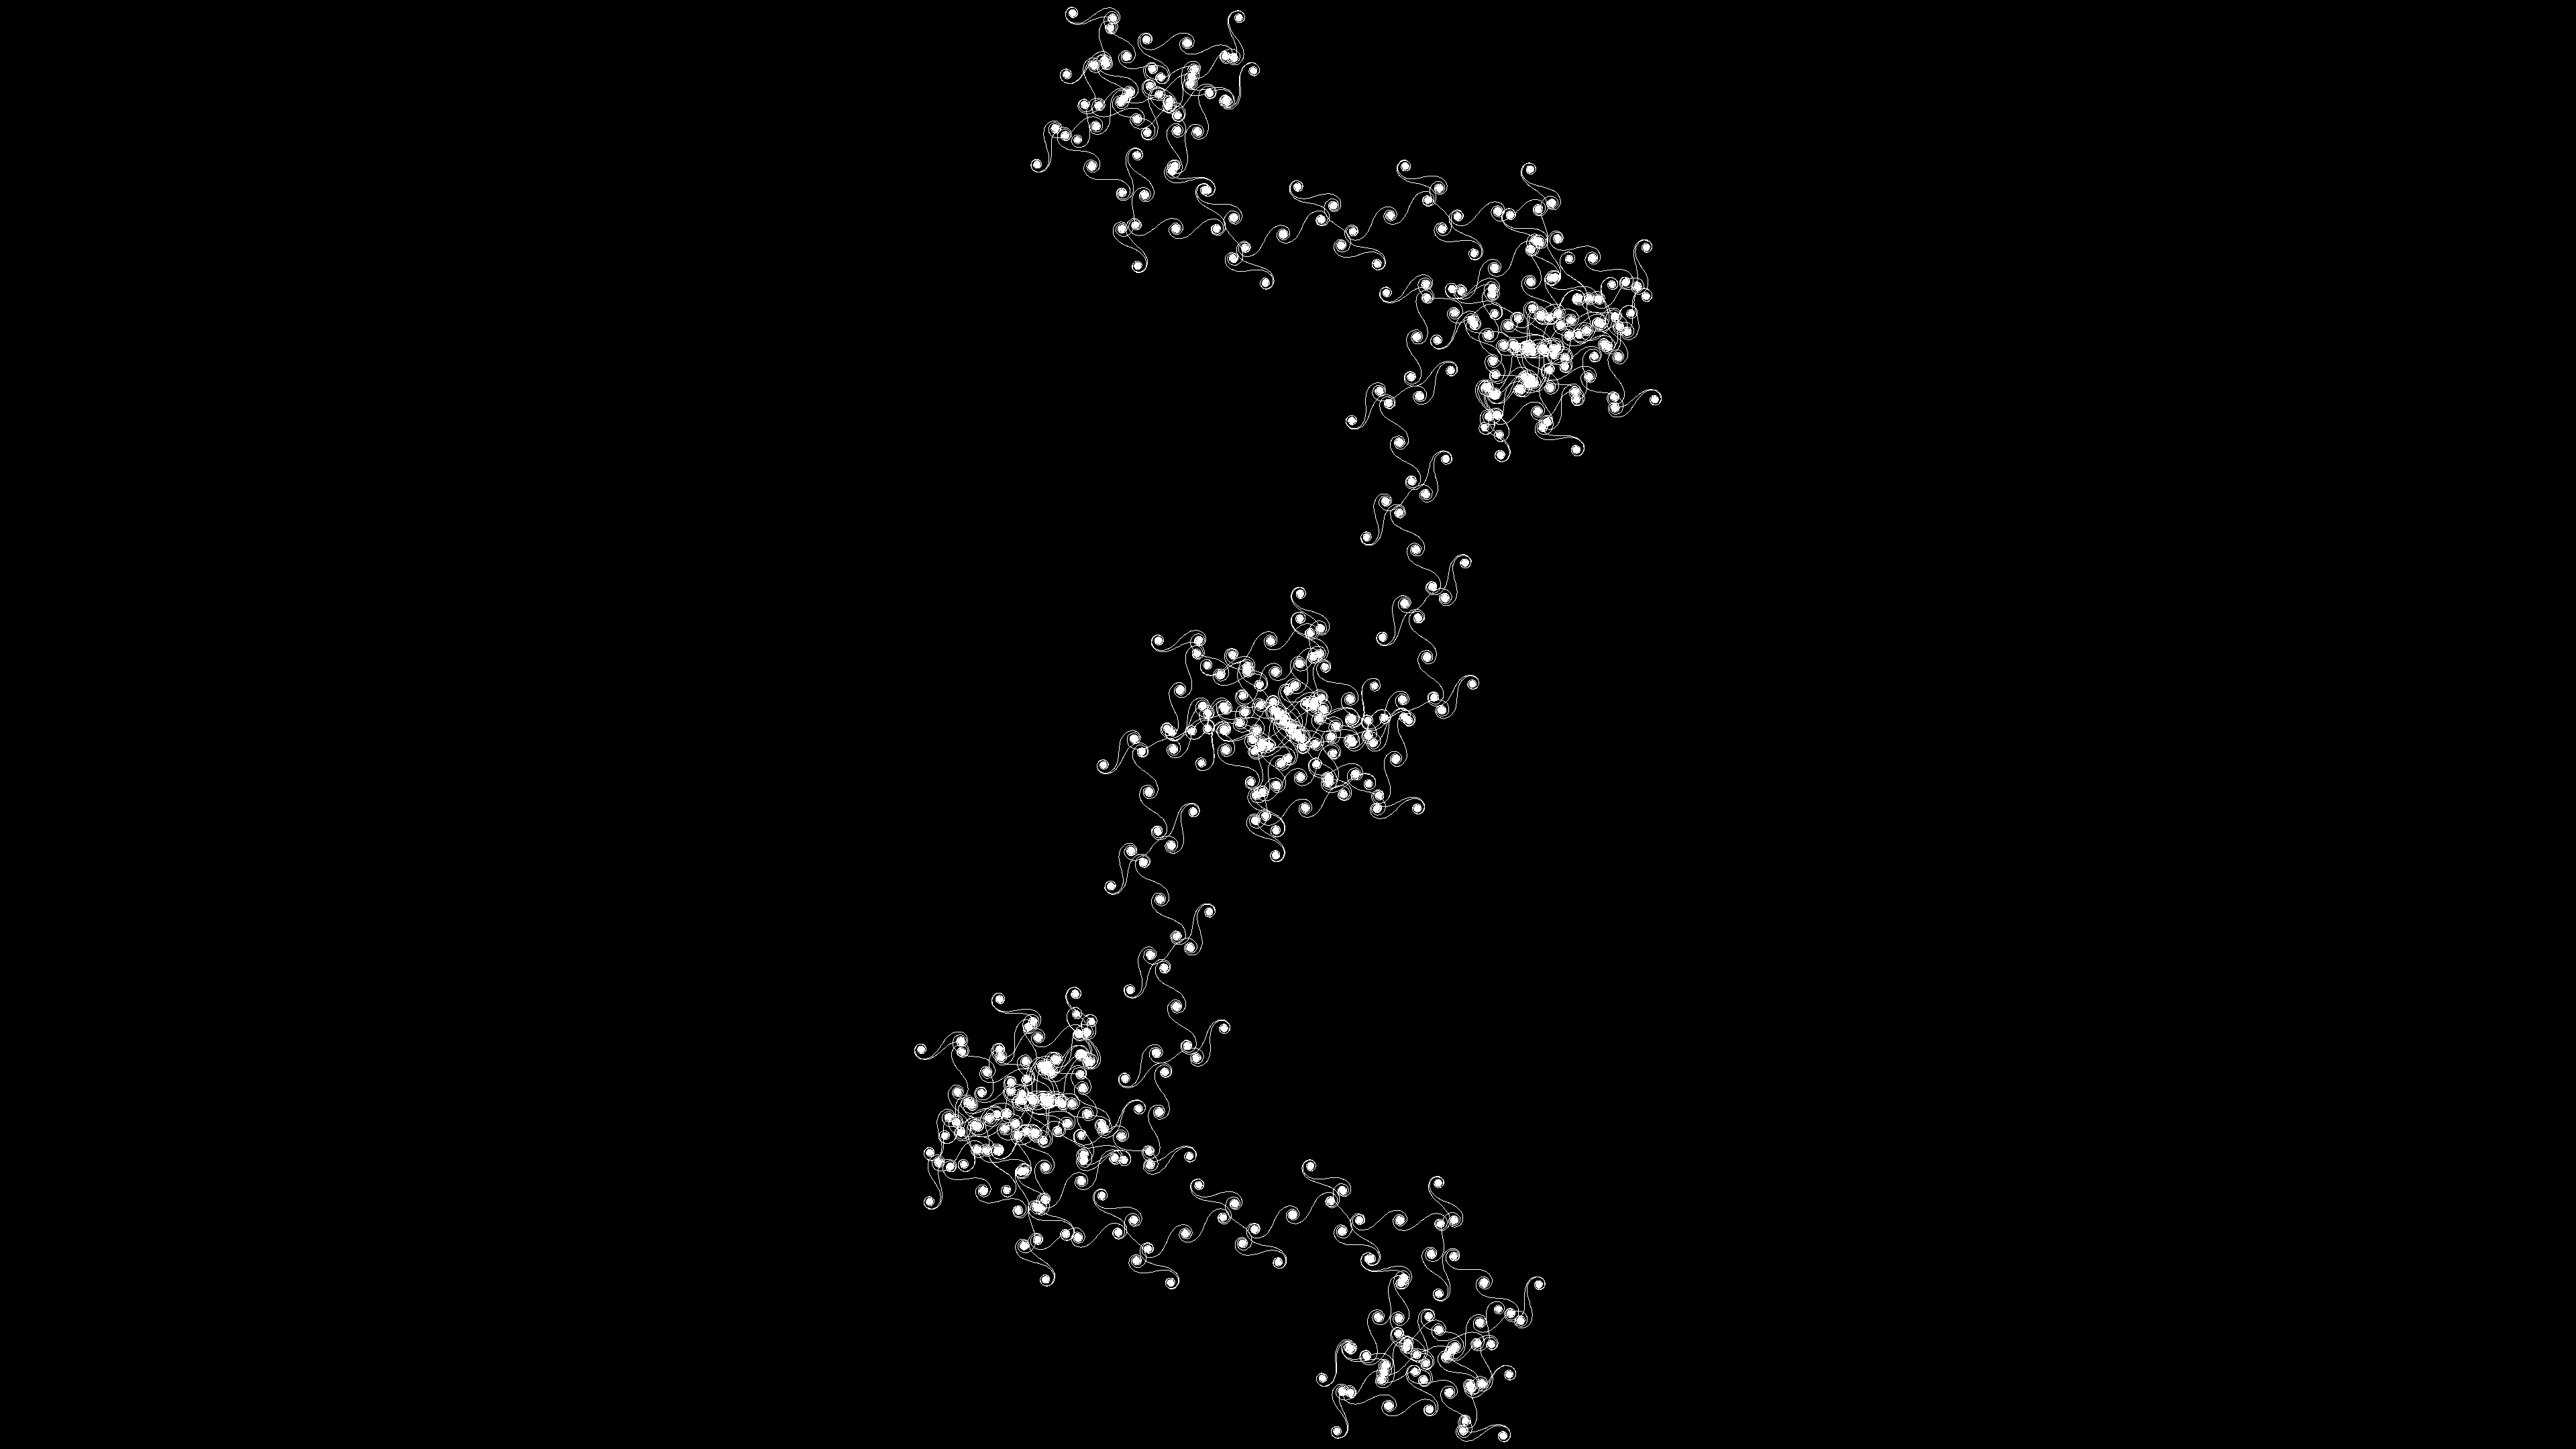
\includegraphics[width=\linewidth]{./stepsplusoneimages/0000000143.png}
    \caption{tf p=499 q=199742 theta=000 89936017.png}
  \end{subfigure}
  \begin{subfigure}[t]{0.48\textwidth}
    \centering
    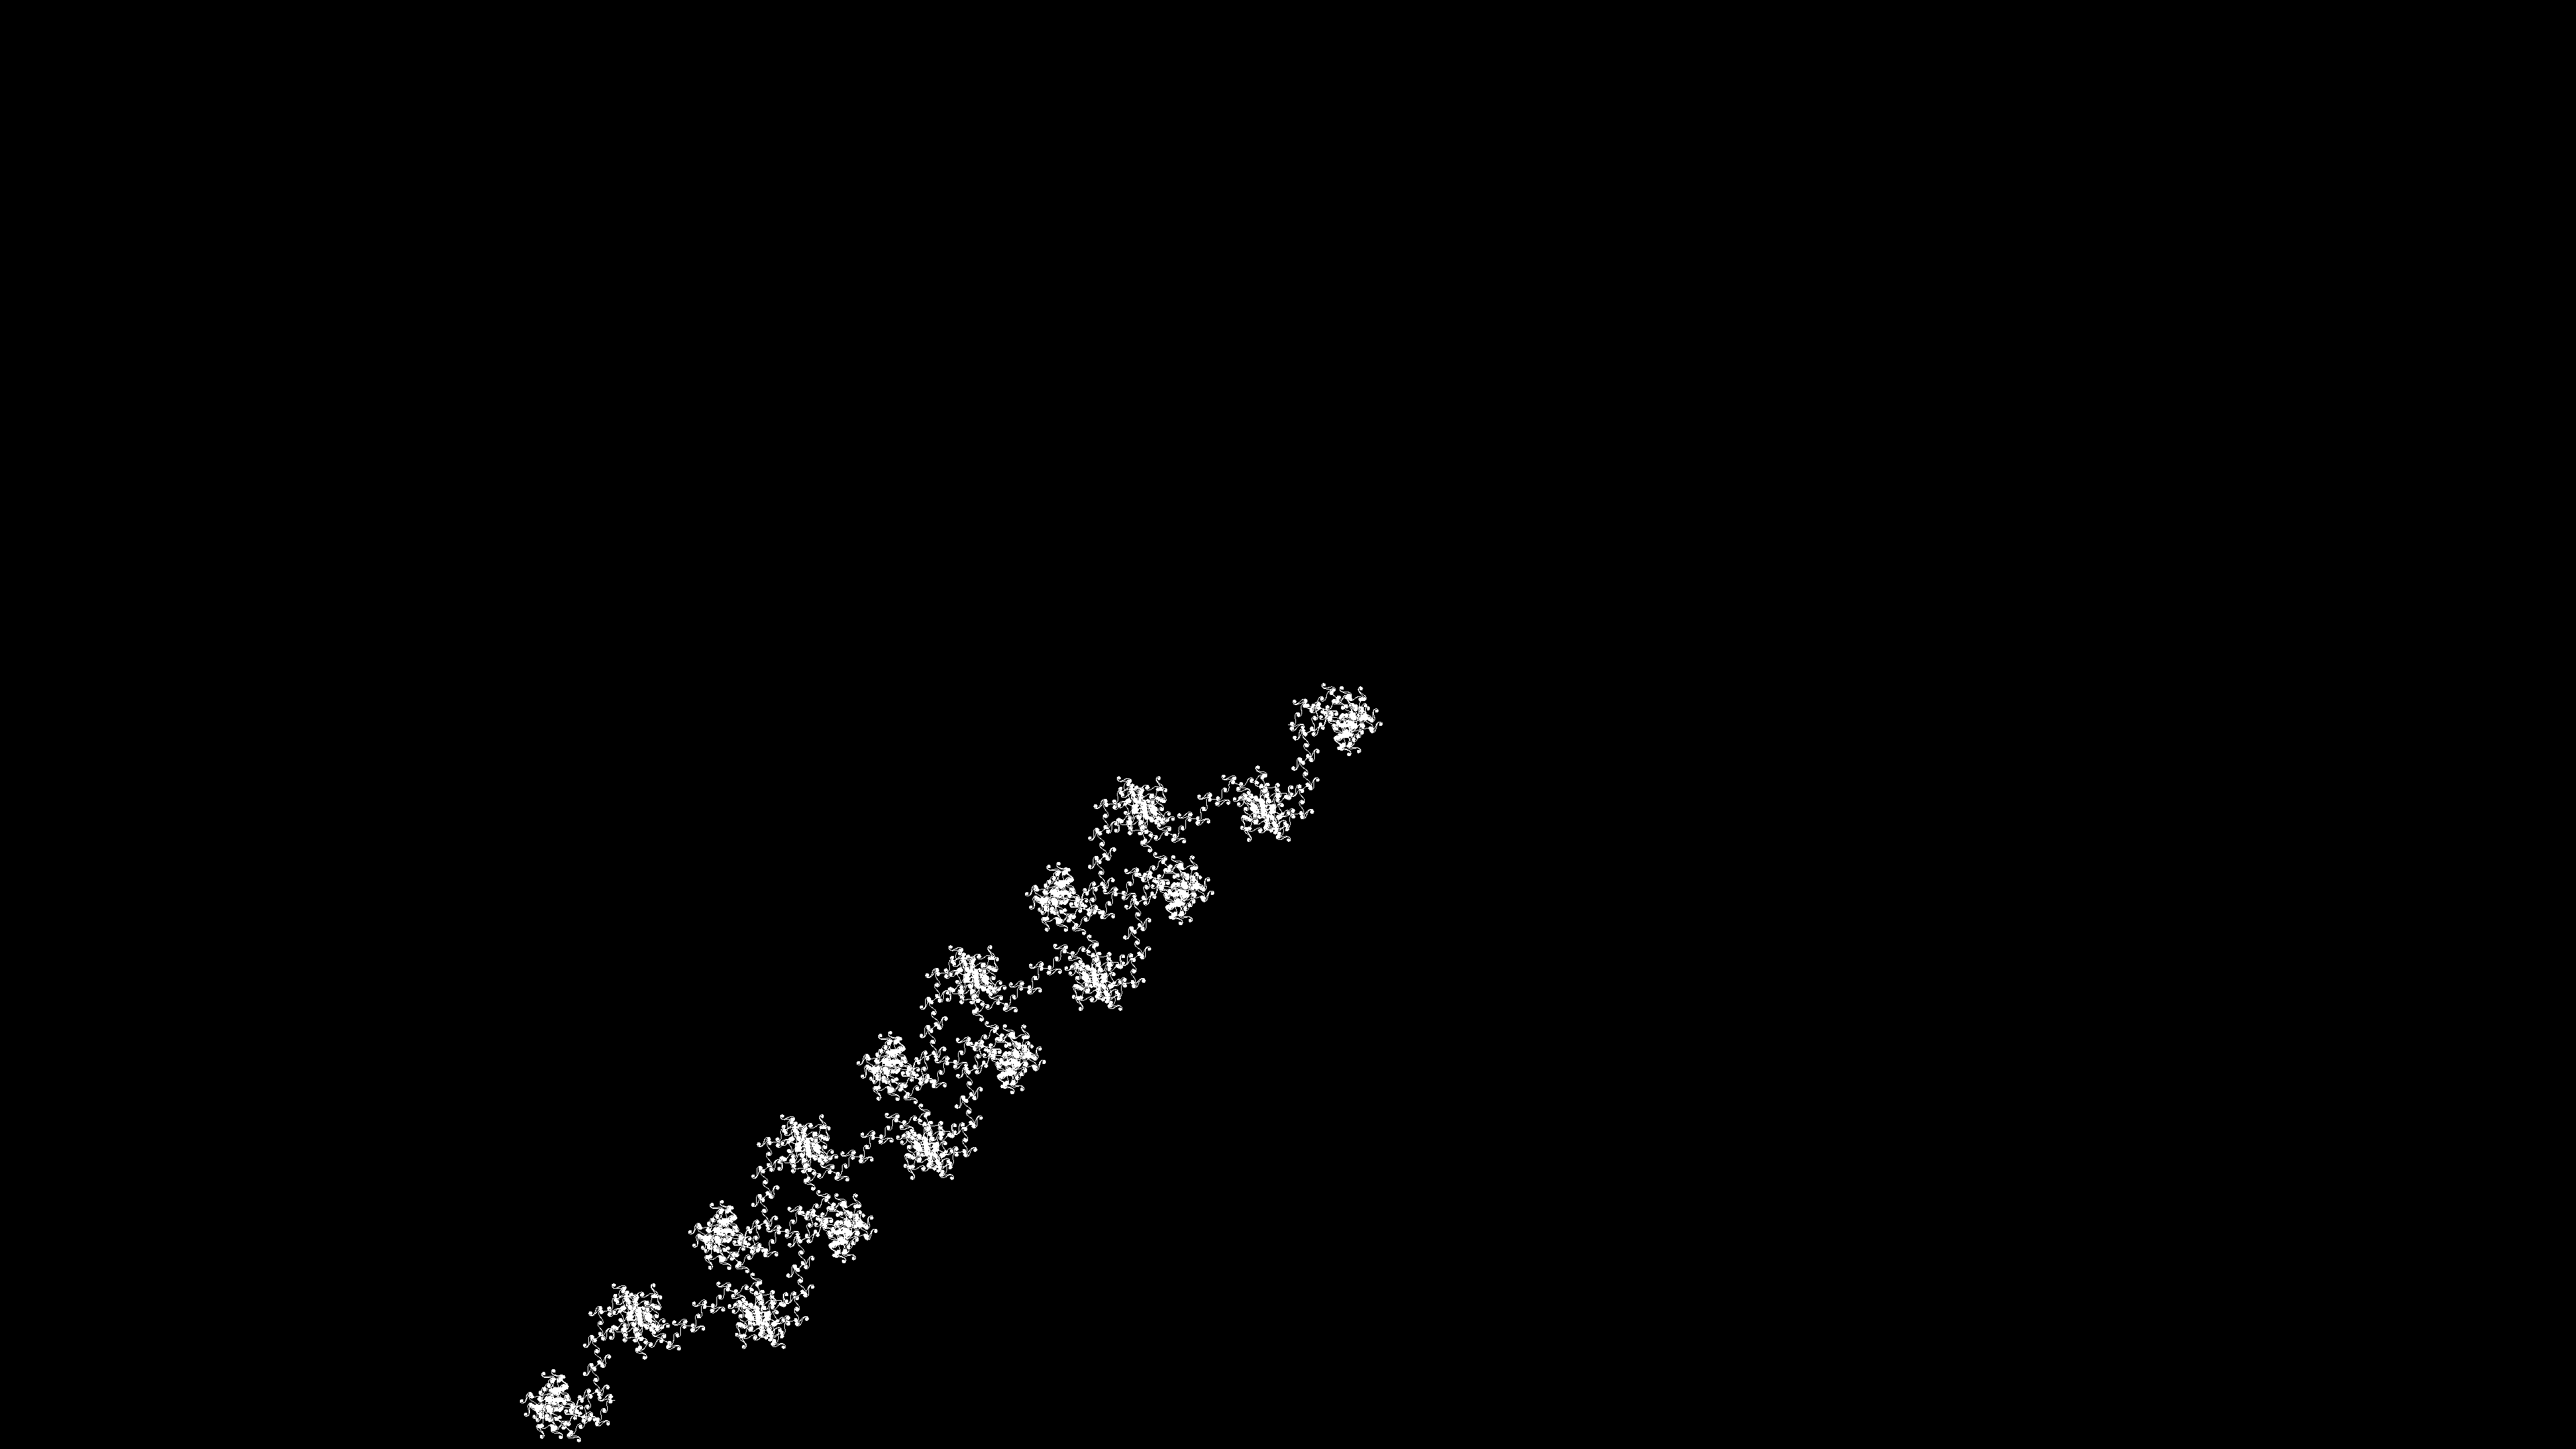
\includegraphics[width=\linewidth]{./stepsplusoneimages/0000000144.png}
    \caption{tf p=499 q=200241 theta=000 89711897.png}
  \end{subfigure}
  \caption{n=142 s=400 s+1=401}
  \label{fig:n=142}
\end{figure}
\begin{figure}[H]
  \centering
  \begin{subfigure}[t]{0.48\textwidth}
    \centering
    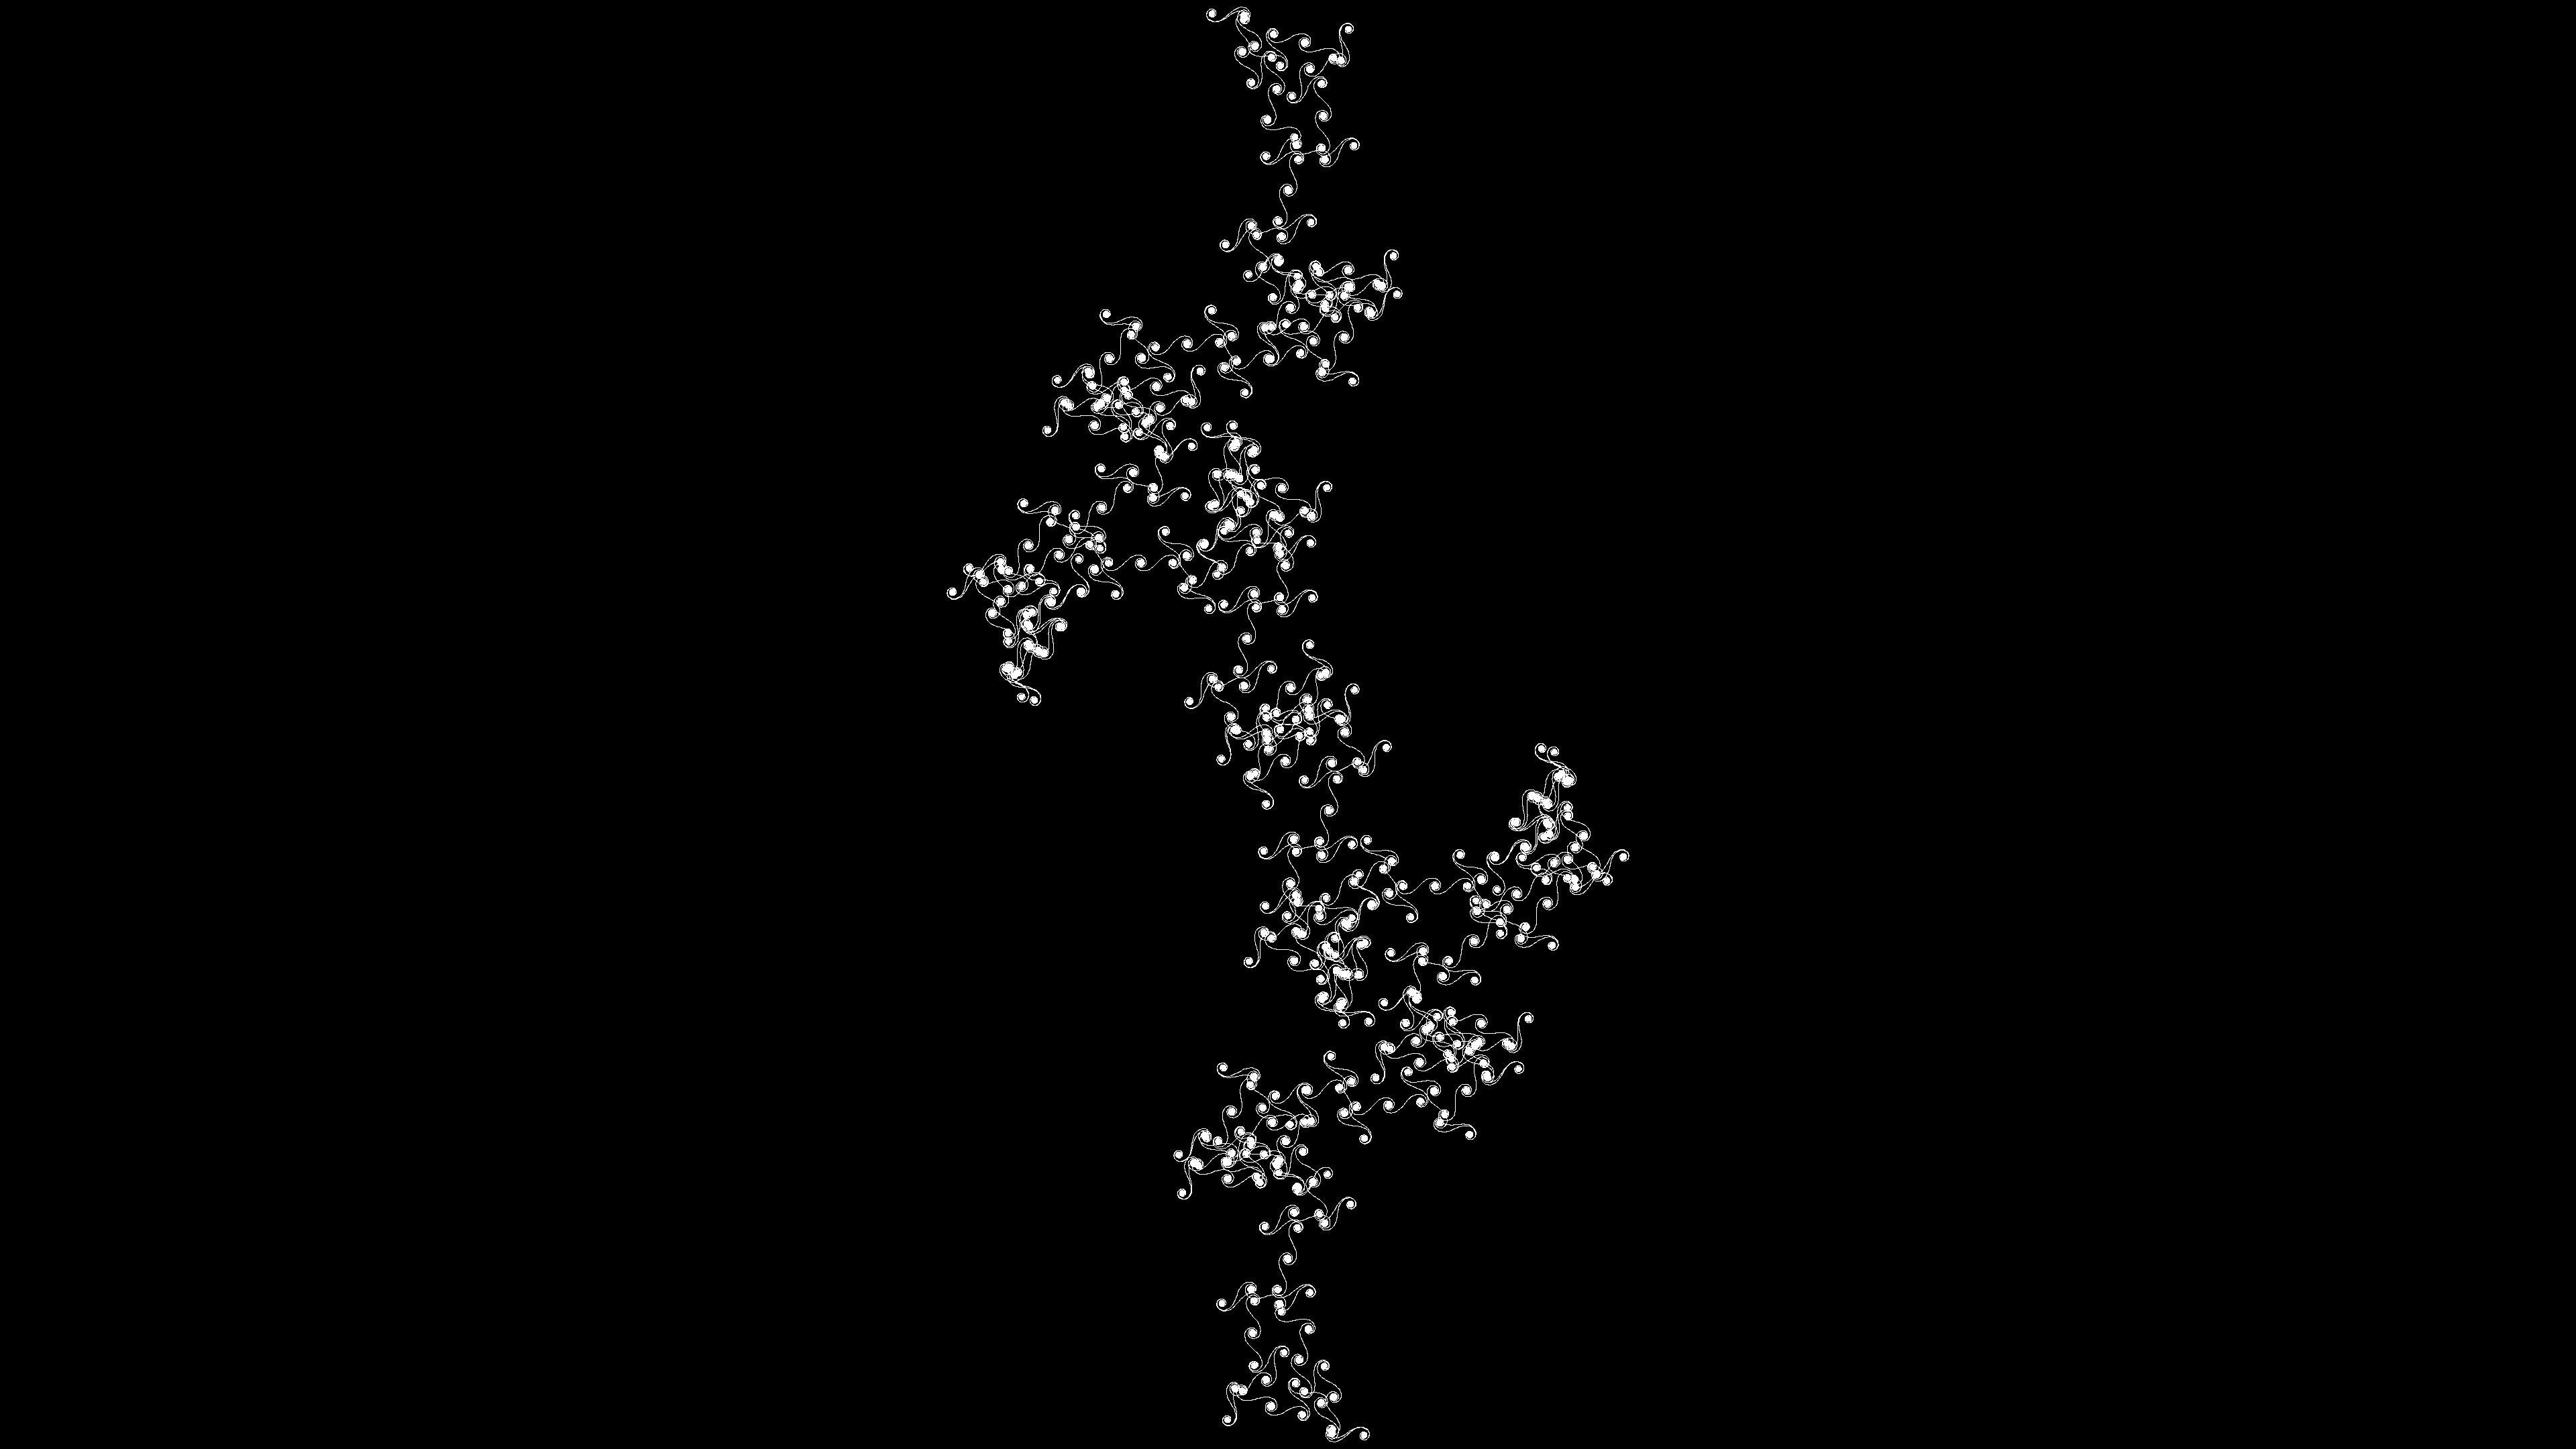
\includegraphics[width=\linewidth]{./stepsplusoneimages/0000000145.png}
    \caption{tf p=499 q=199744 theta=000 89935117.png}
  \end{subfigure}
  \begin{subfigure}[t]{0.48\textwidth}
    \centering
    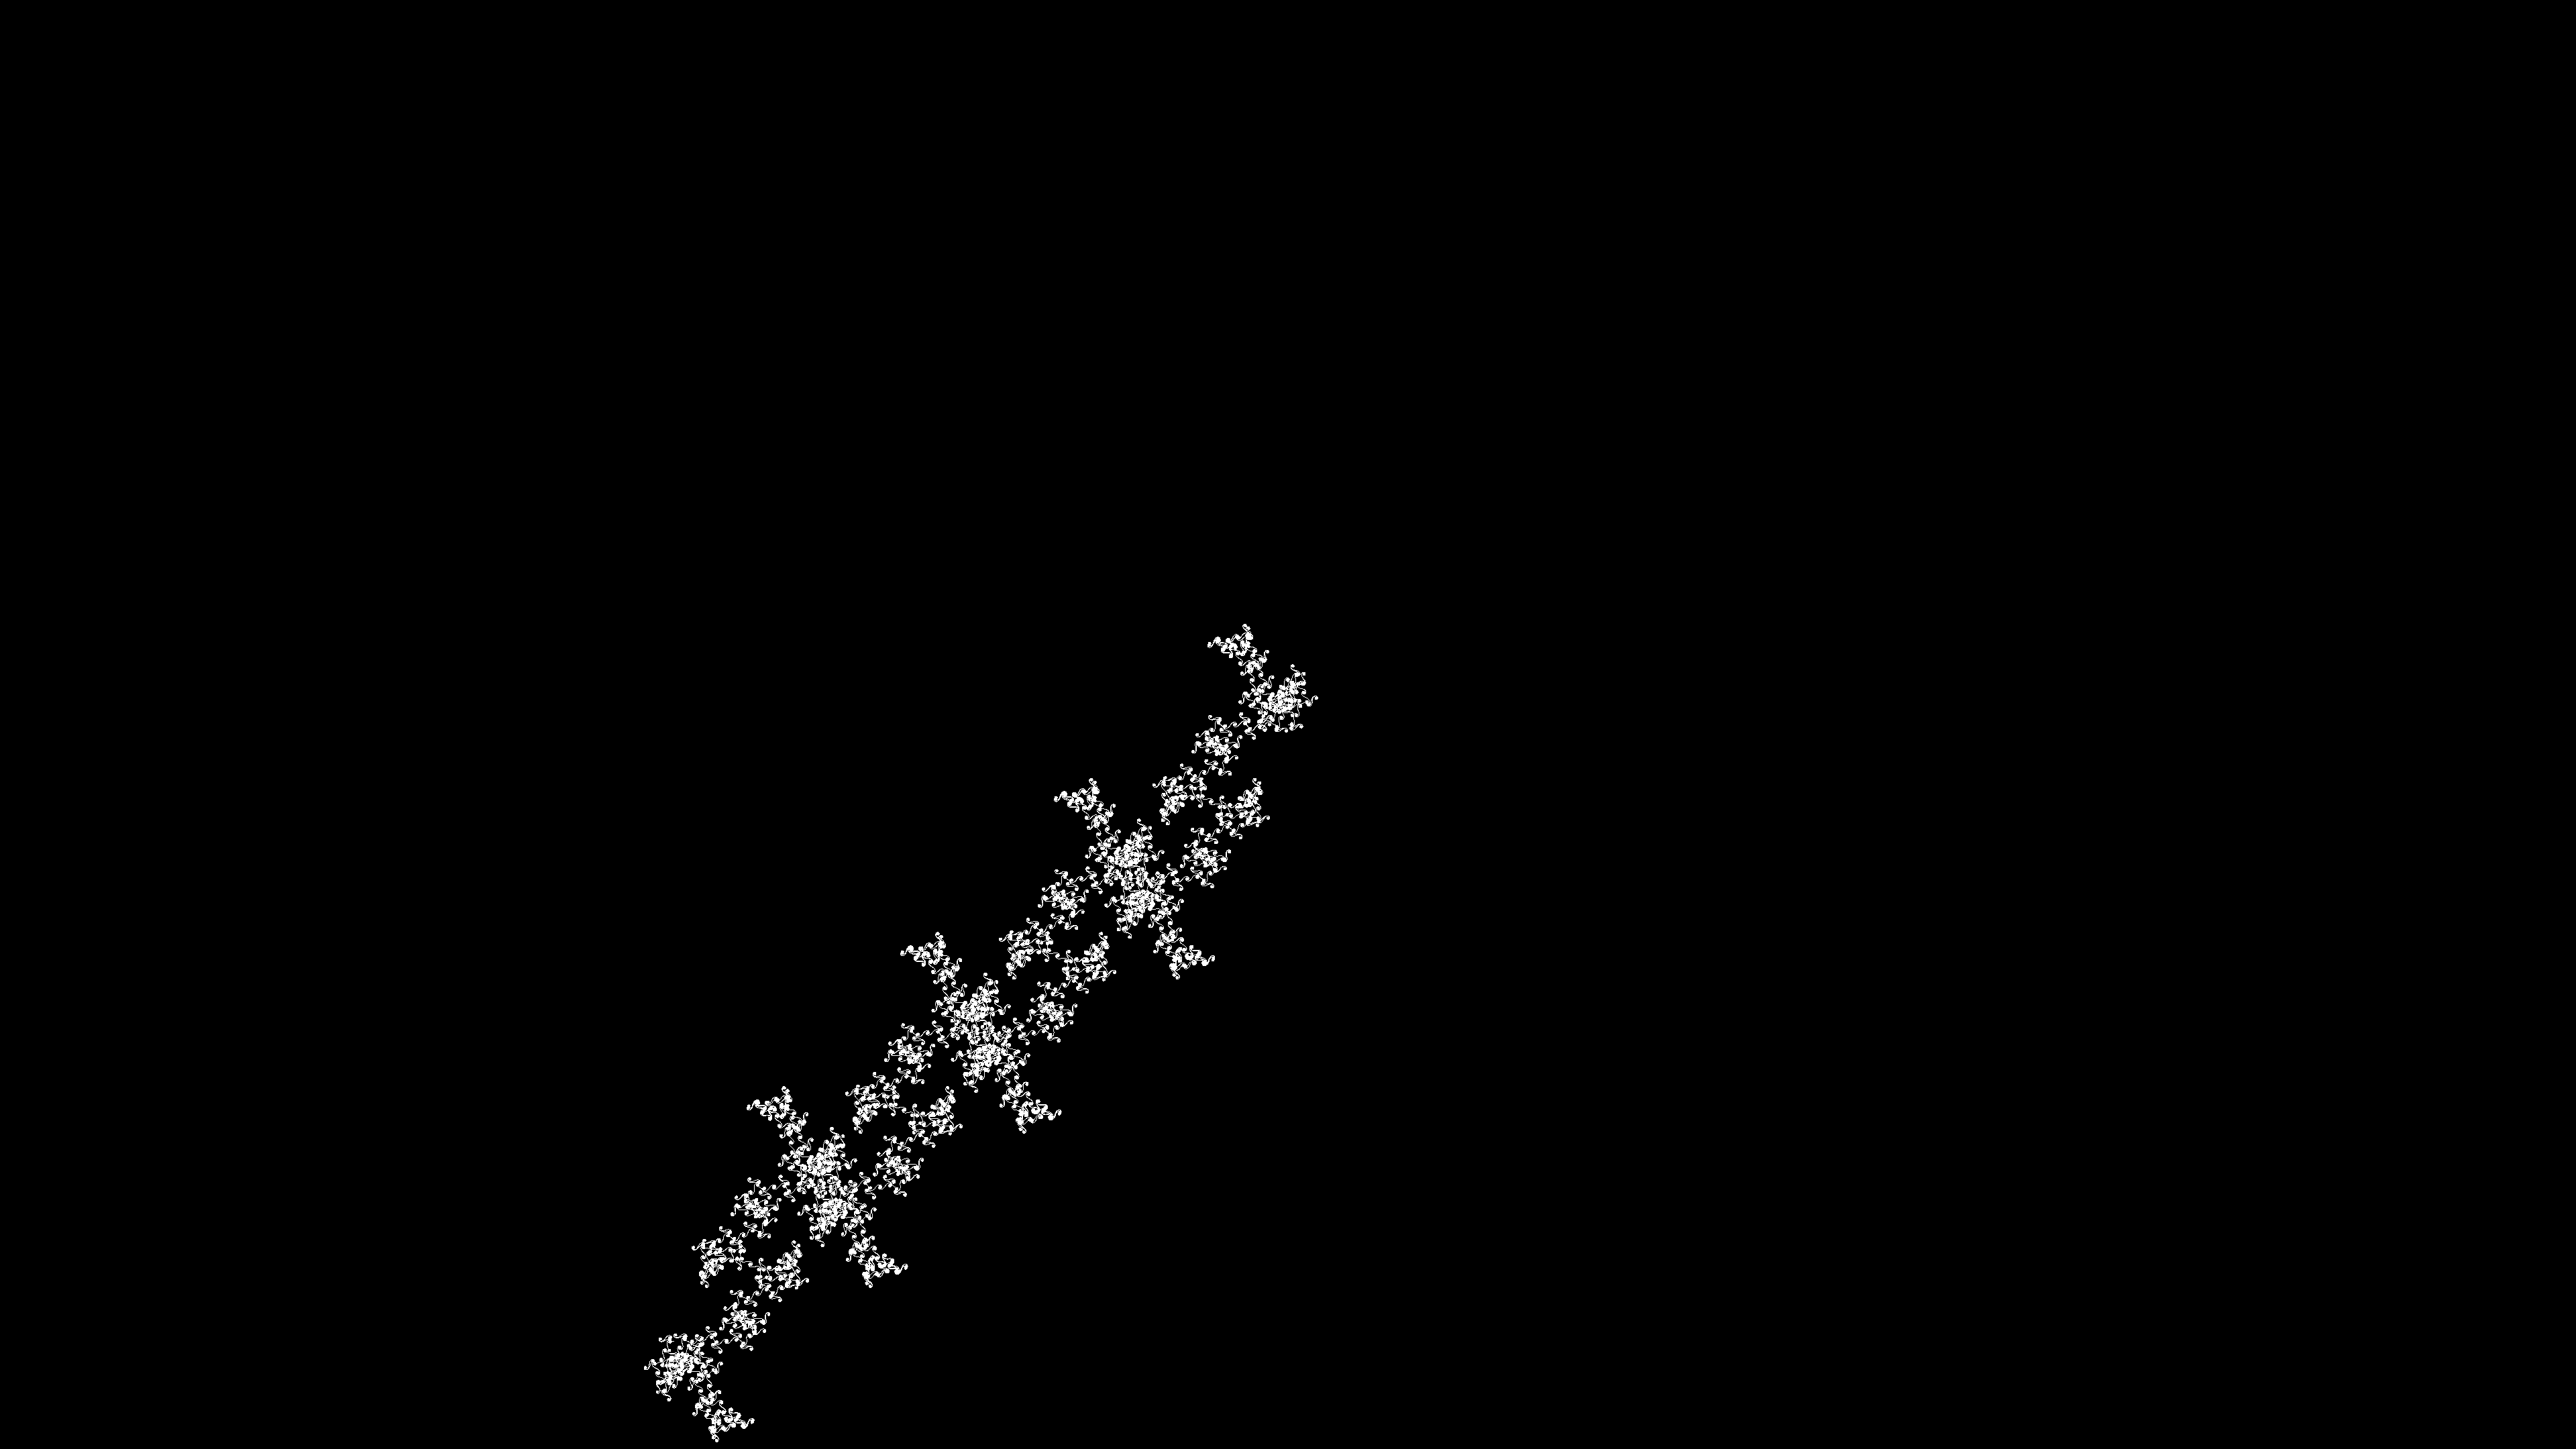
\includegraphics[width=\linewidth]{./stepsplusoneimages/0000000146.png}
    \caption{tf p=499 q=200243 theta=000 89711001.png}
  \end{subfigure}
  \caption{n=144 s=400 s+1=401}
  \label{fig:n=144}
\end{figure}
\begin{figure}[H]
  \centering
  \begin{subfigure}[t]{0.48\textwidth}
    \centering
    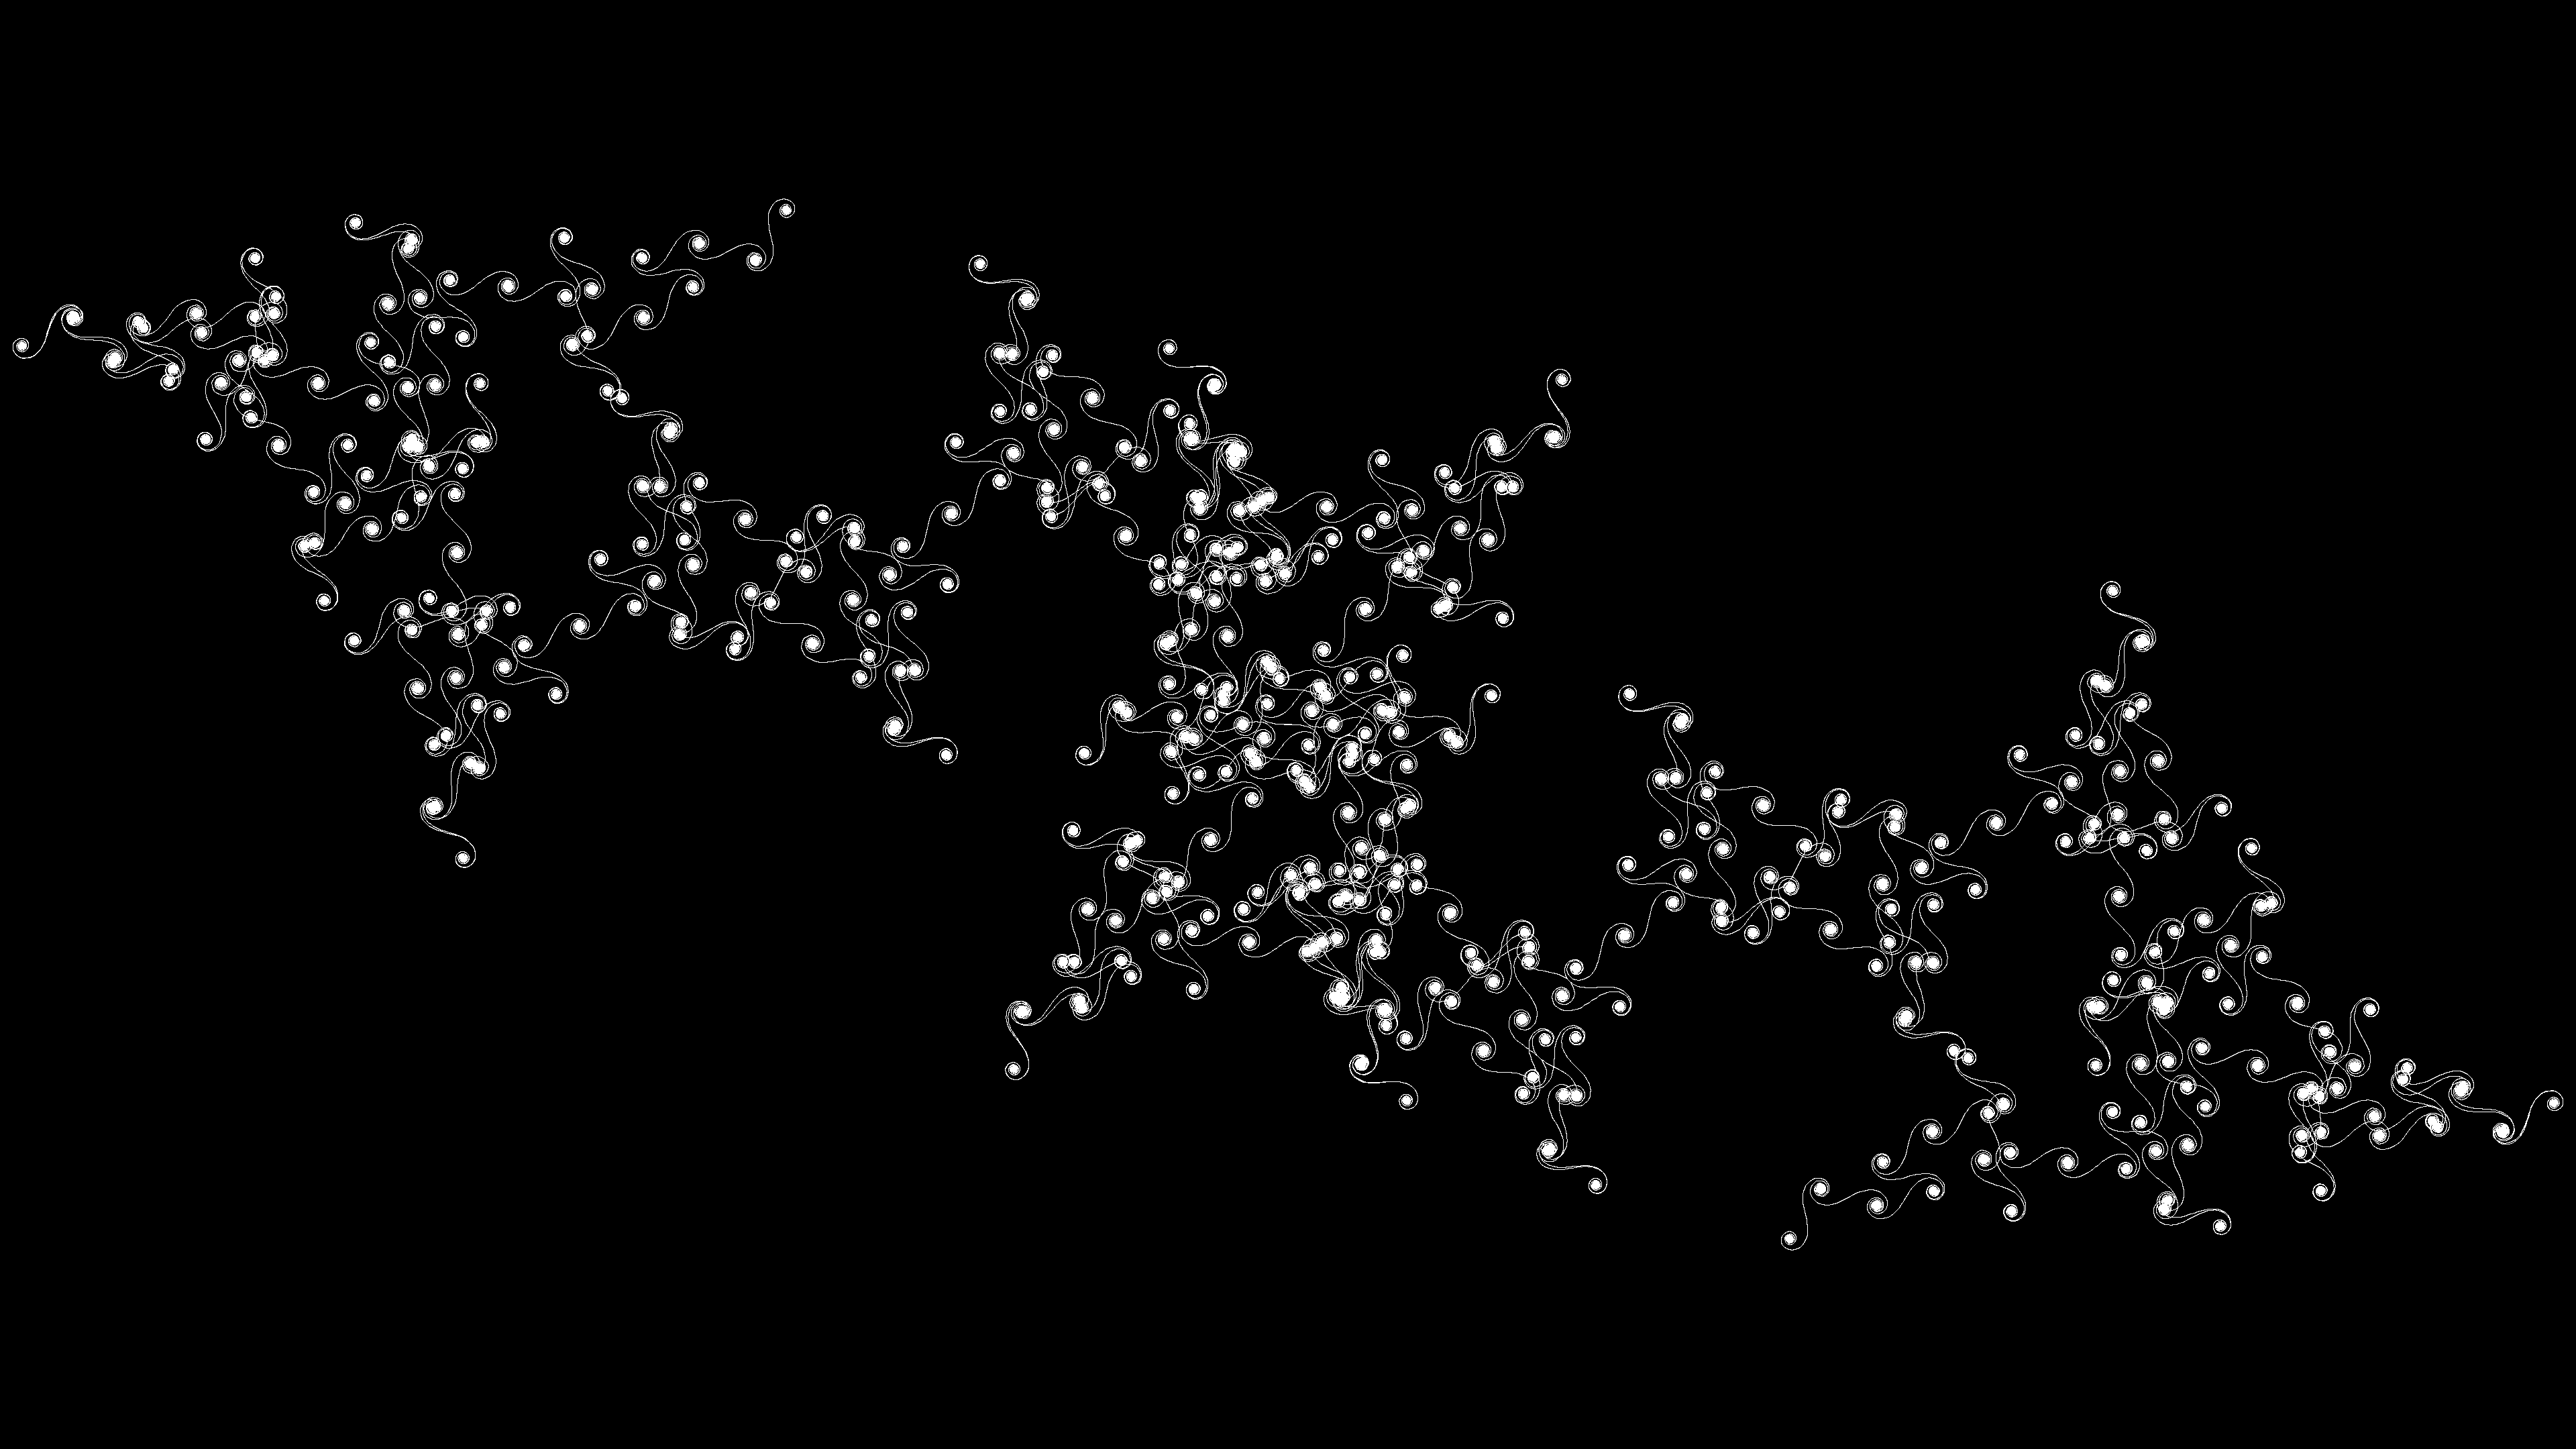
\includegraphics[width=\linewidth]{./stepsplusoneimages/0000000147.png}
    \caption{tf p=499 q=199746 theta=000 89934216.png}
  \end{subfigure}
  \begin{subfigure}[t]{0.48\textwidth}
    \centering
    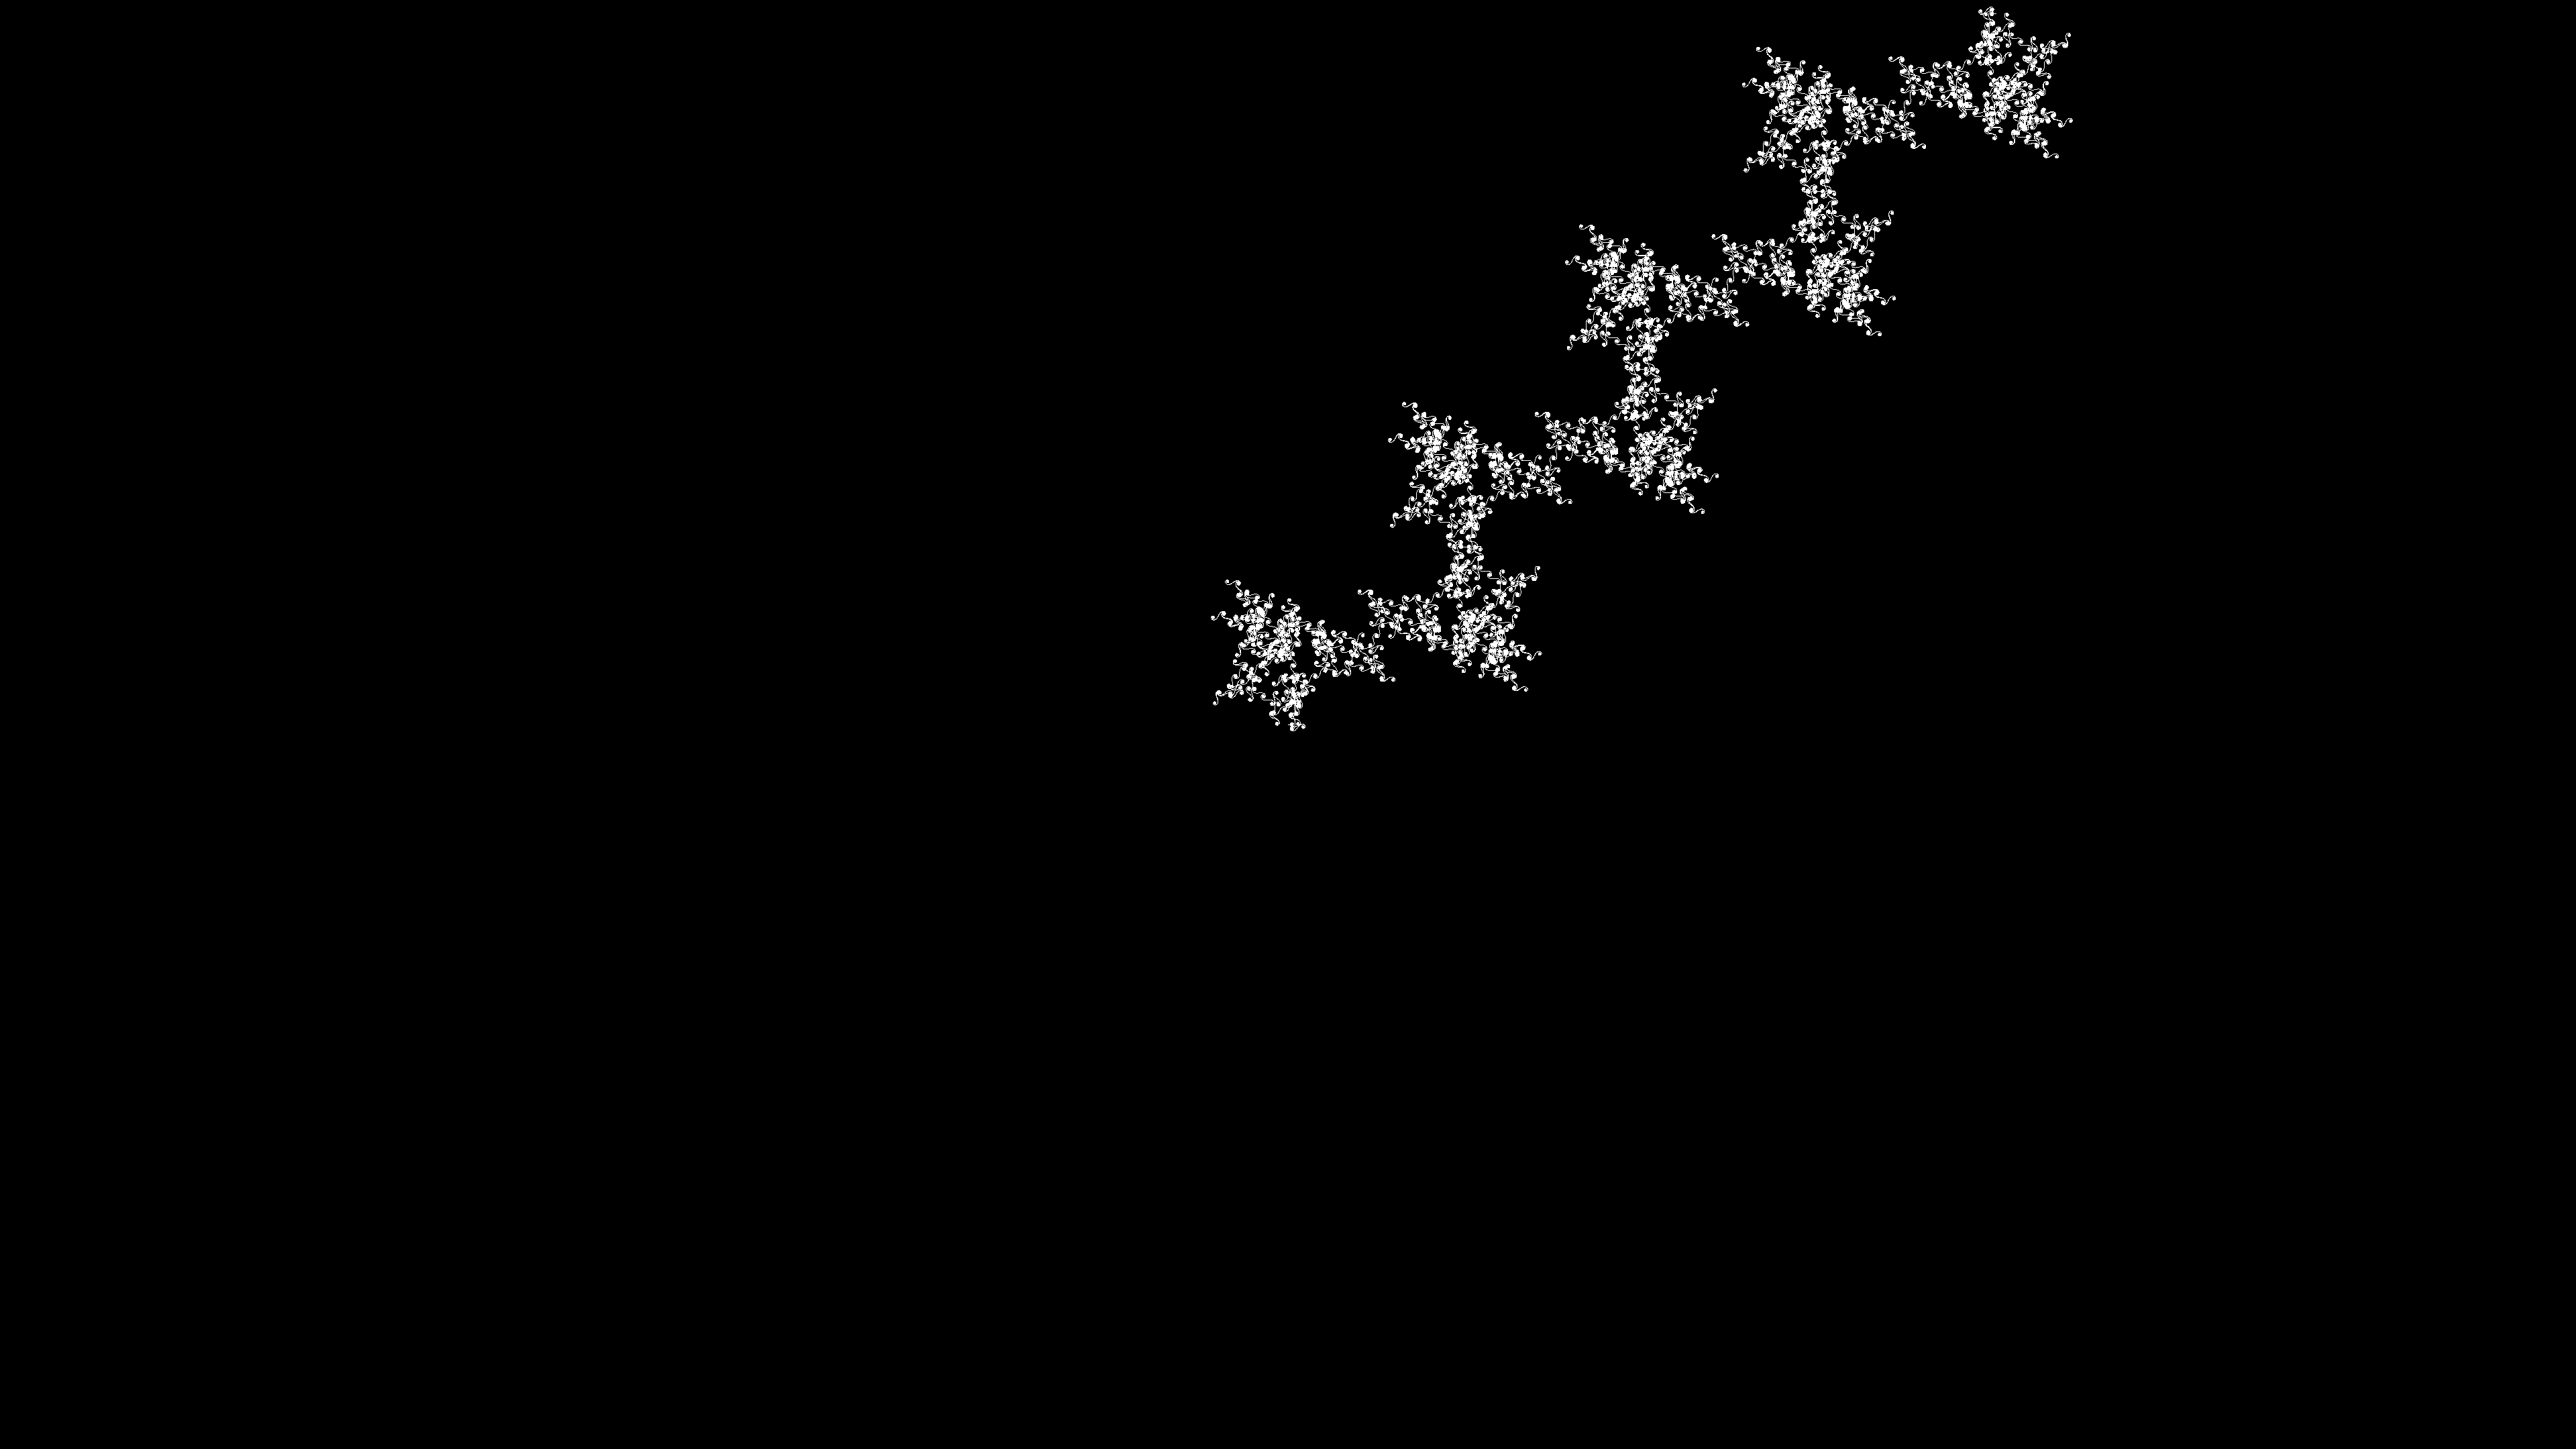
\includegraphics[width=\linewidth]{./stepsplusoneimages/0000000148.png}
    \caption{tf p=499 q=200245 theta=000 89710105.png}
  \end{subfigure}
  \caption{n=146 s=400 s+1=401}
  \label{fig:n=146}
\end{figure}
\begin{figure}[H]
  \centering
  \begin{subfigure}[t]{0.48\textwidth}
    \centering
    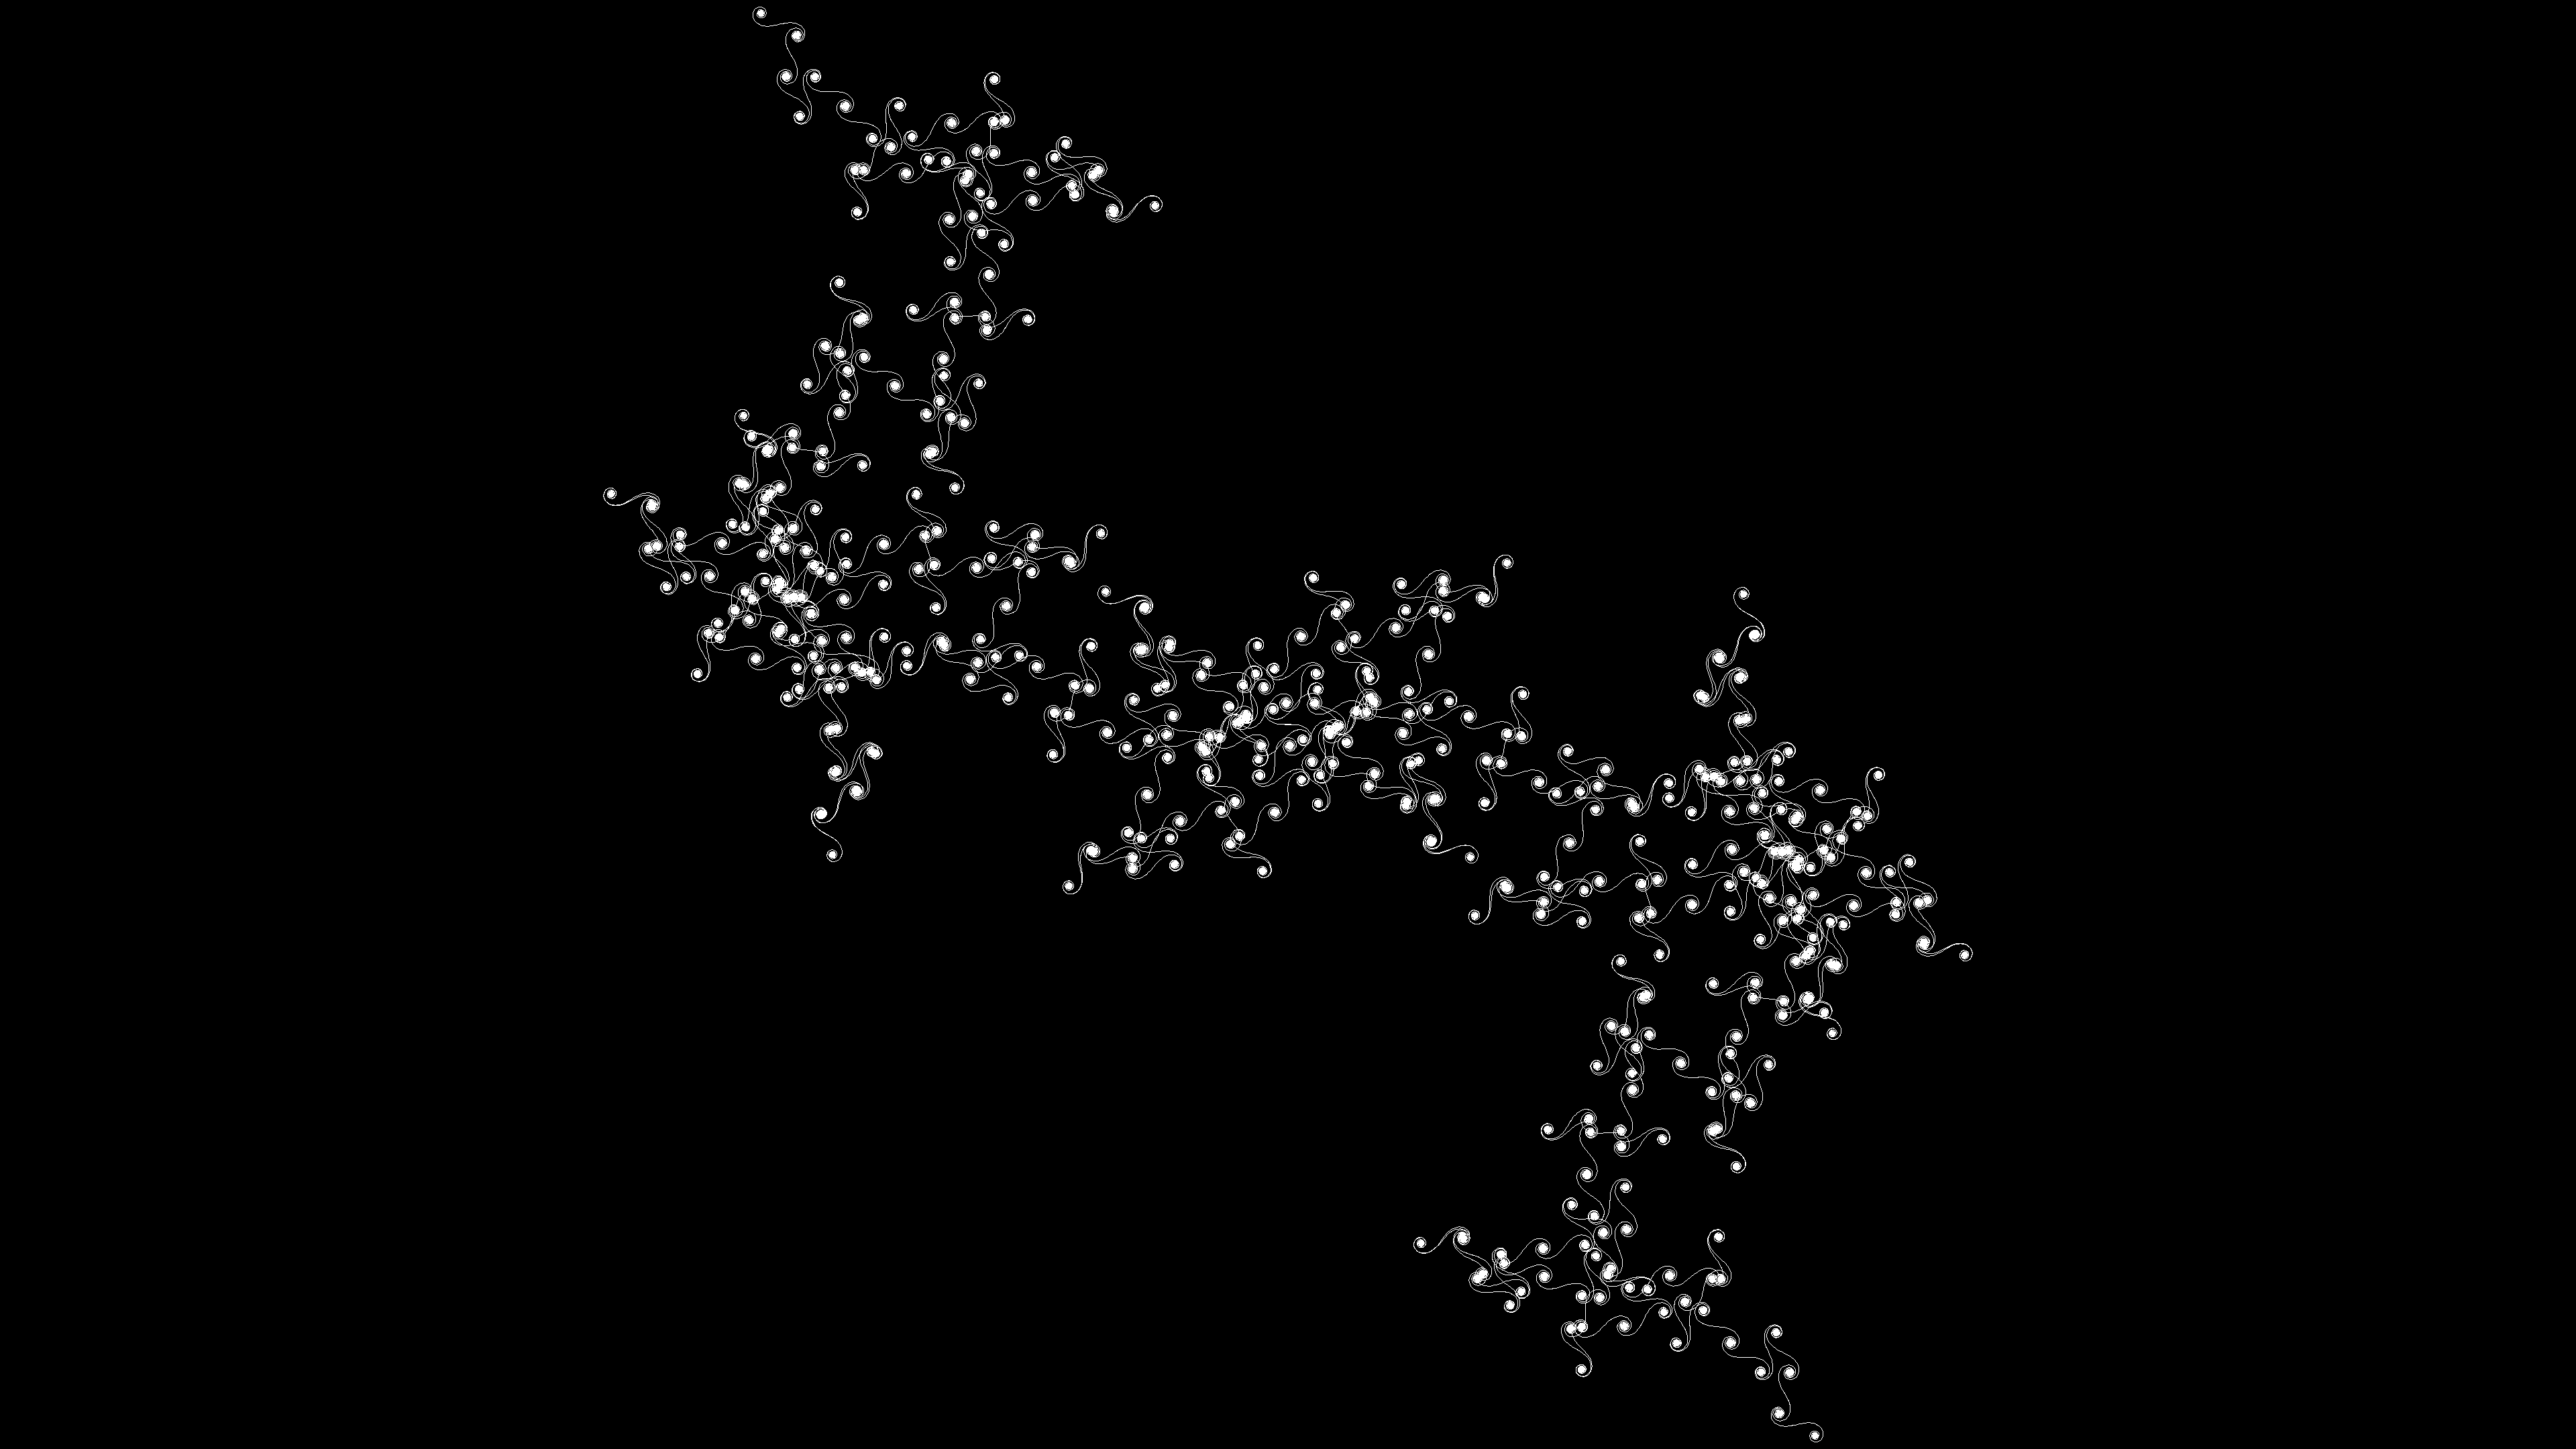
\includegraphics[width=\linewidth]{./stepsplusoneimages/0000000149.png}
    \caption{tf p=499 q=199748 theta=000 89933316.png}
  \end{subfigure}
  \begin{subfigure}[t]{0.48\textwidth}
    \centering
    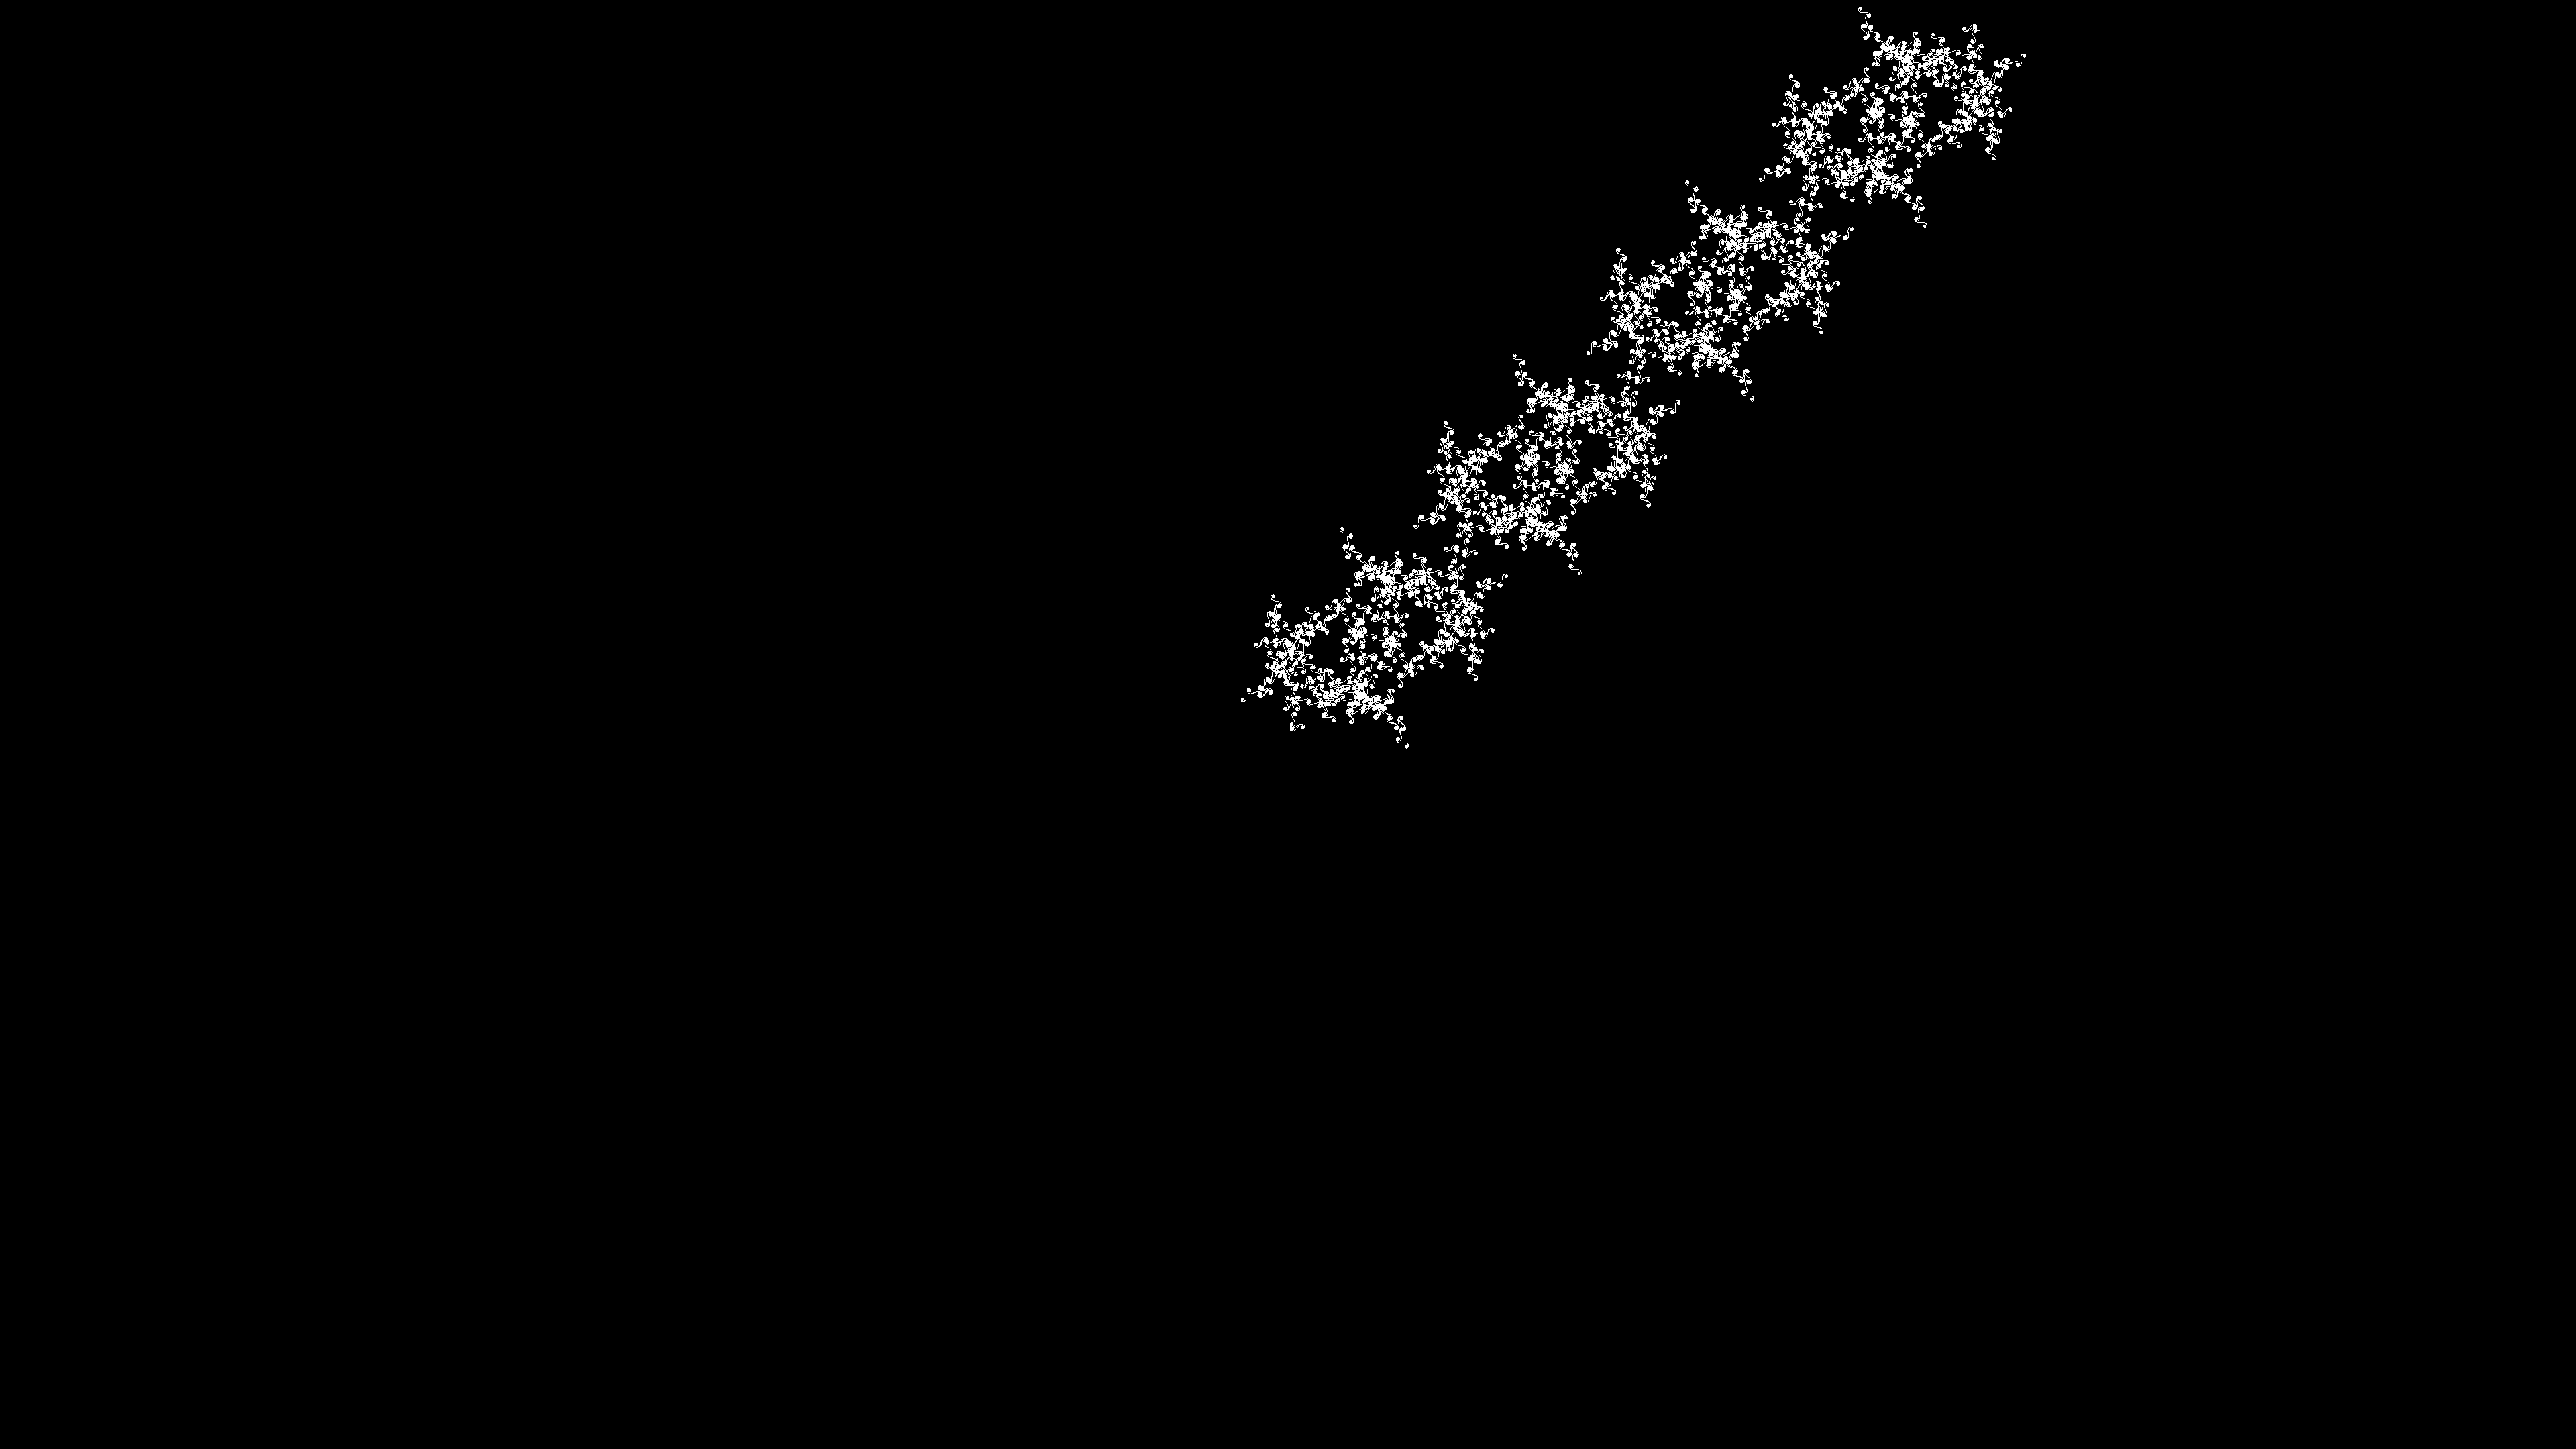
\includegraphics[width=\linewidth]{./stepsplusoneimages/0000000150.png}
    \caption{tf p=499 q=200247 theta=000 89709209.png}
  \end{subfigure}
  \caption{n=148 s=400 s+1=401}
  \label{fig:n=148}
\end{figure}
\begin{figure}[H]
  \centering
  \begin{subfigure}[t]{0.48\textwidth}
    \centering
    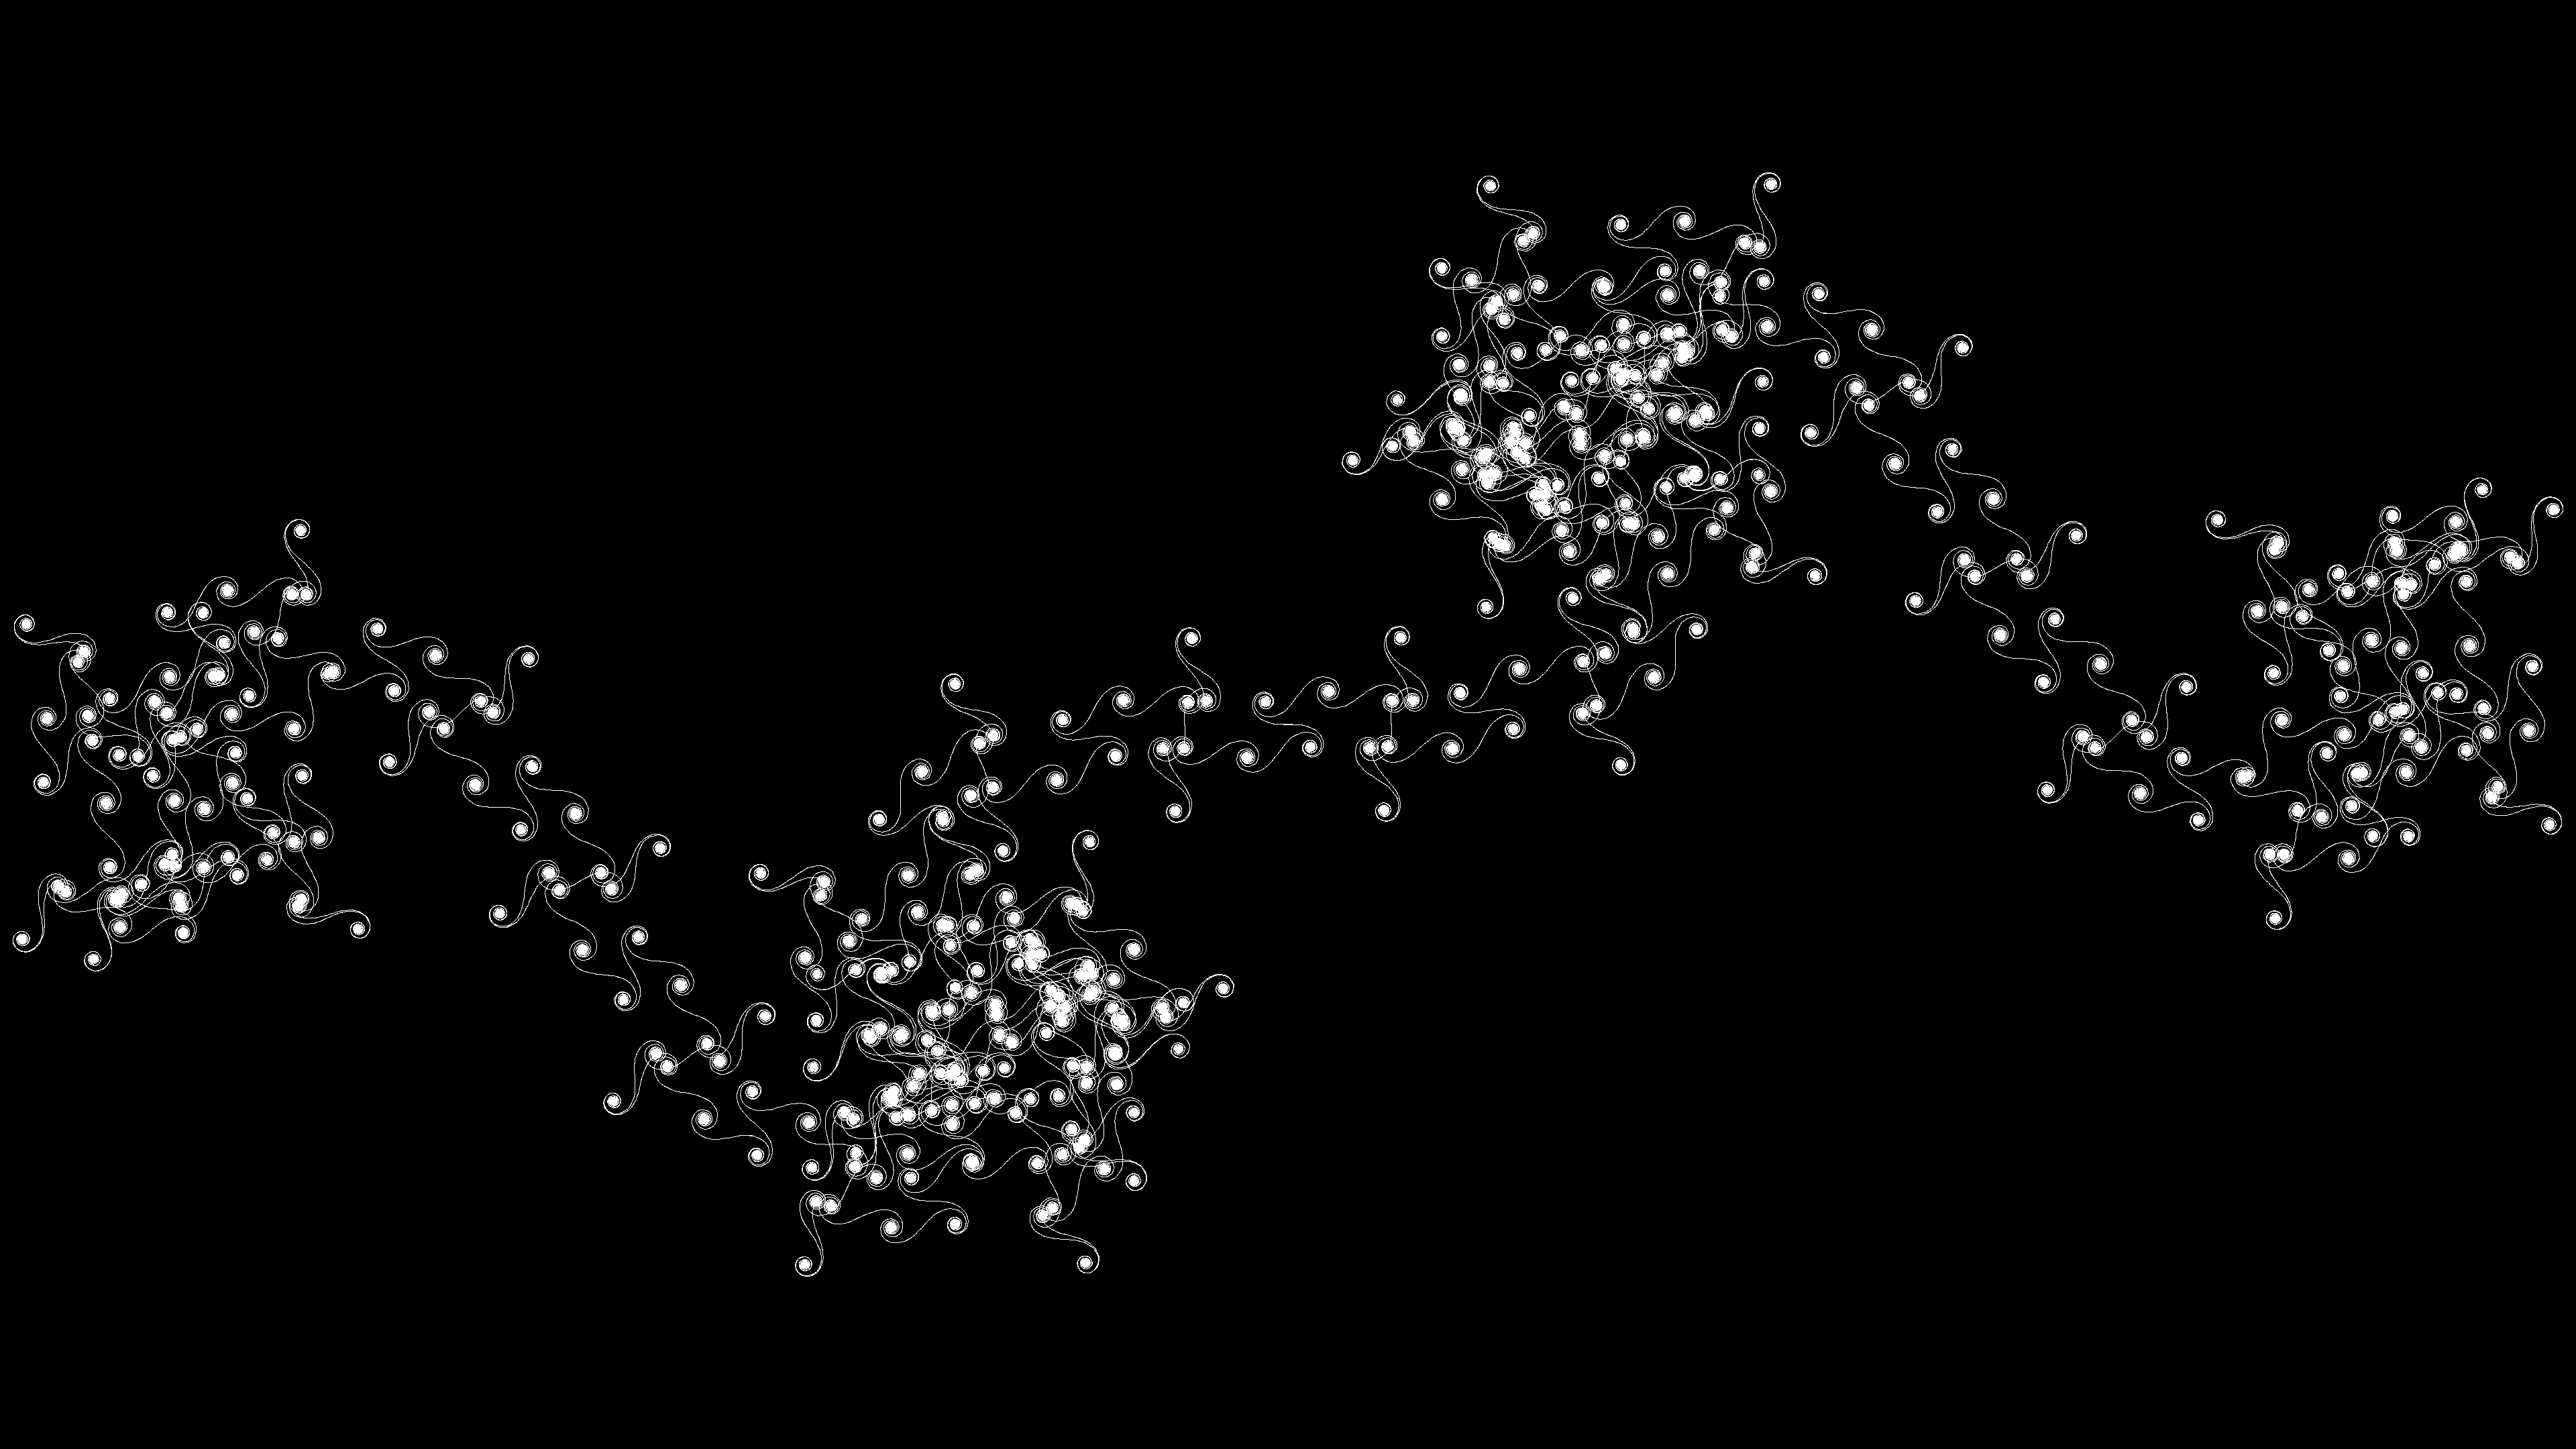
\includegraphics[width=\linewidth]{./stepsplusoneimages/0000000151.png}
    \caption{tf p=499 q=199750 theta=000 89932416.png}
  \end{subfigure}
  \begin{subfigure}[t]{0.48\textwidth}
    \centering
    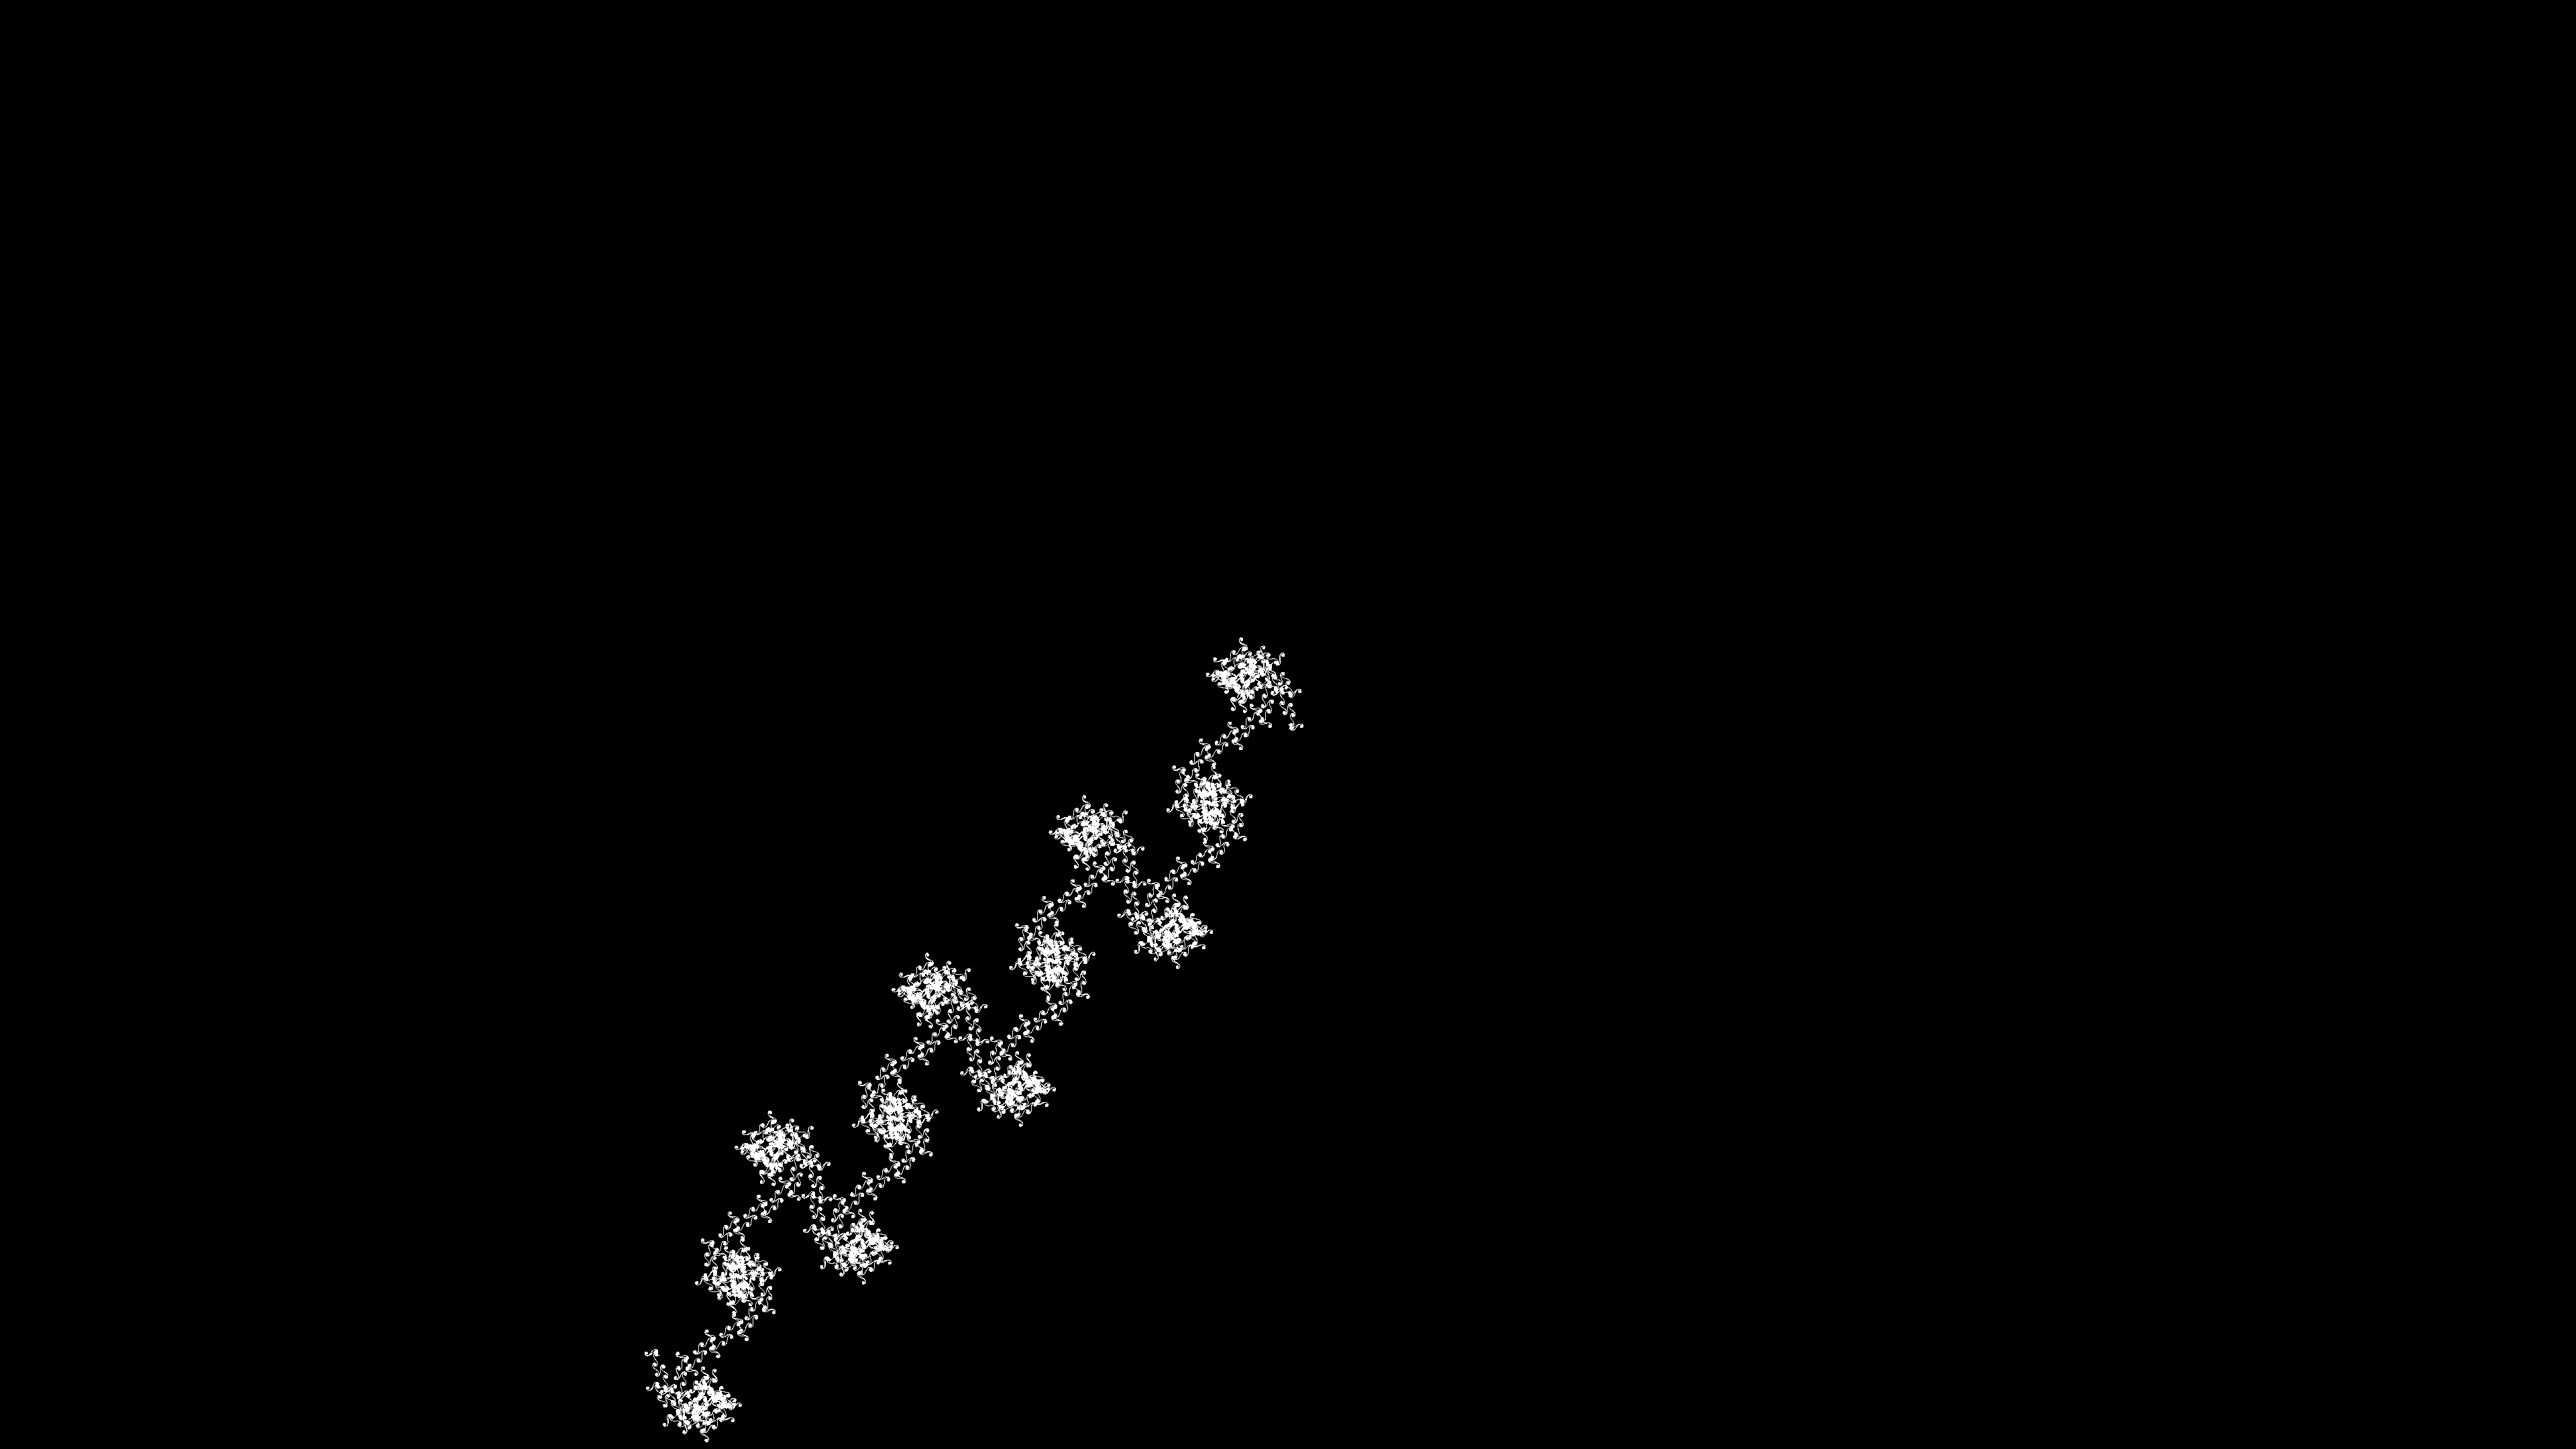
\includegraphics[width=\linewidth]{./stepsplusoneimages/0000000152.png}
    \caption{tf p=499 q=200249 theta=000 89708313.png}
  \end{subfigure}
  \caption{n=150 s=400 s+1=401}
  \label{fig:n=150}
\end{figure}
\begin{figure}[H]
  \centering
  \begin{subfigure}[t]{0.48\textwidth}
    \centering
    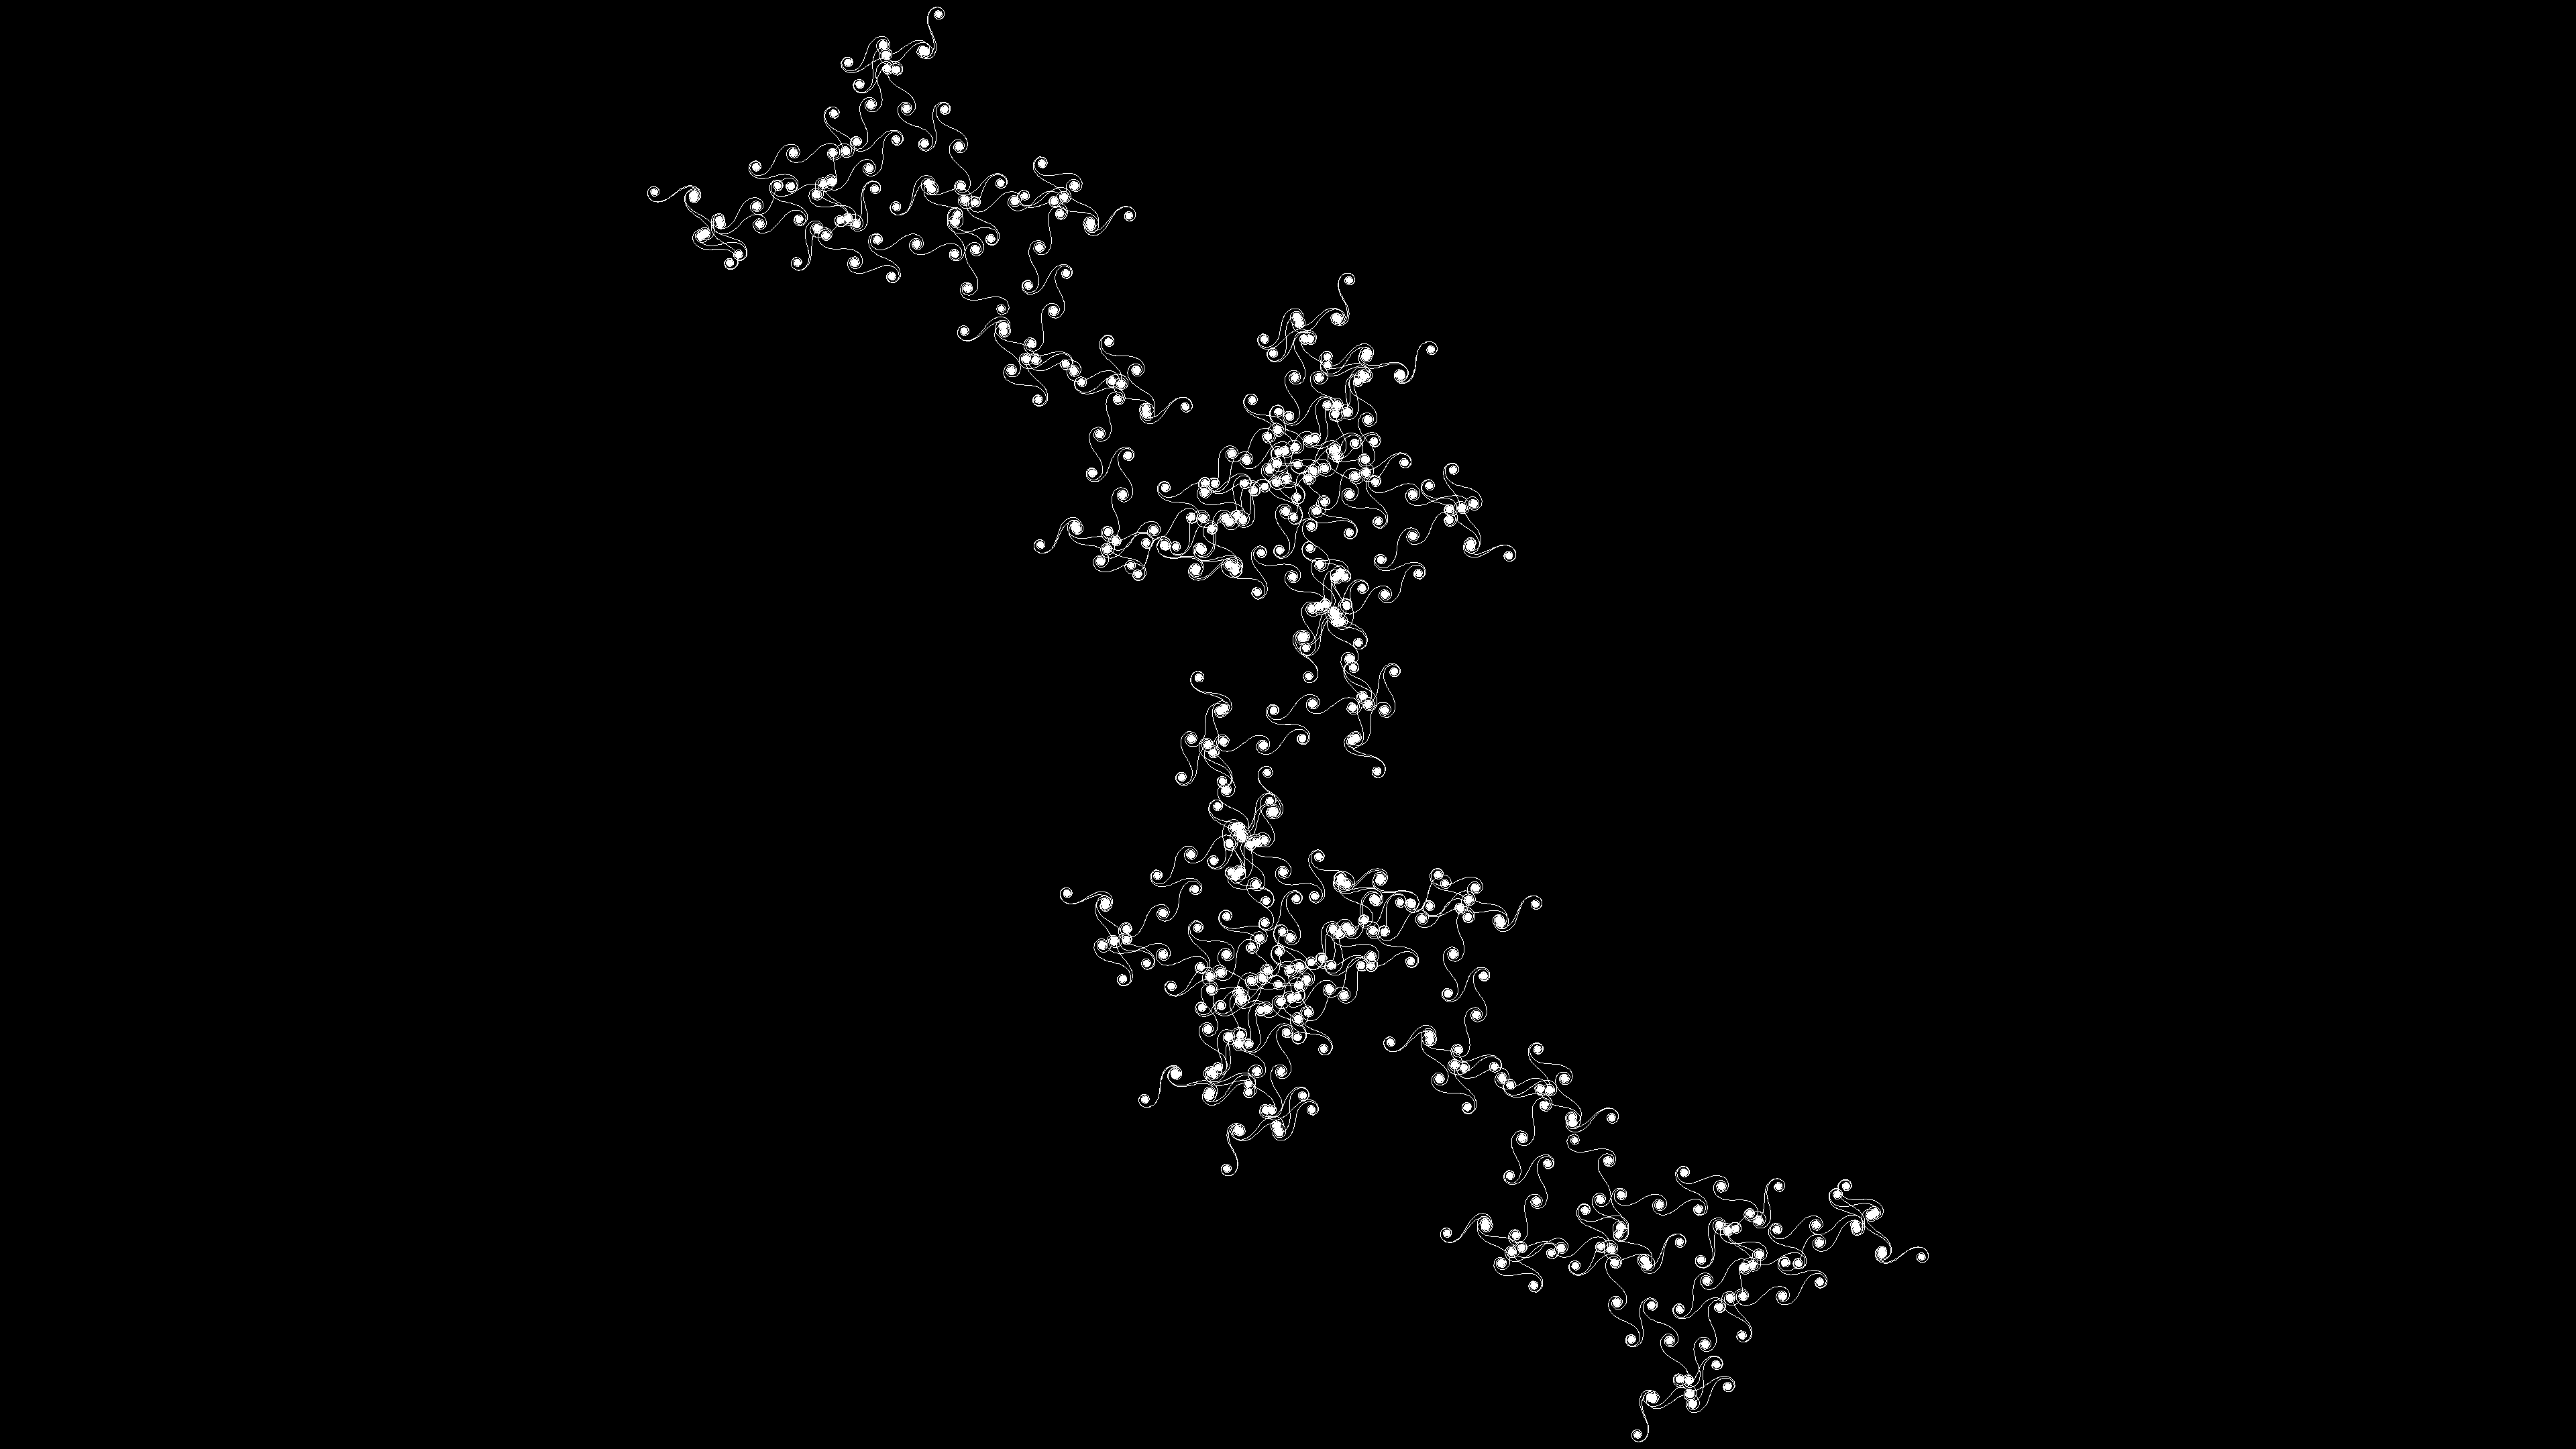
\includegraphics[width=\linewidth]{./stepsplusoneimages/0000000153.png}
    \caption{tf p=499 q=199752 theta=000 89931515.png}
  \end{subfigure}
  \begin{subfigure}[t]{0.48\textwidth}
    \centering
    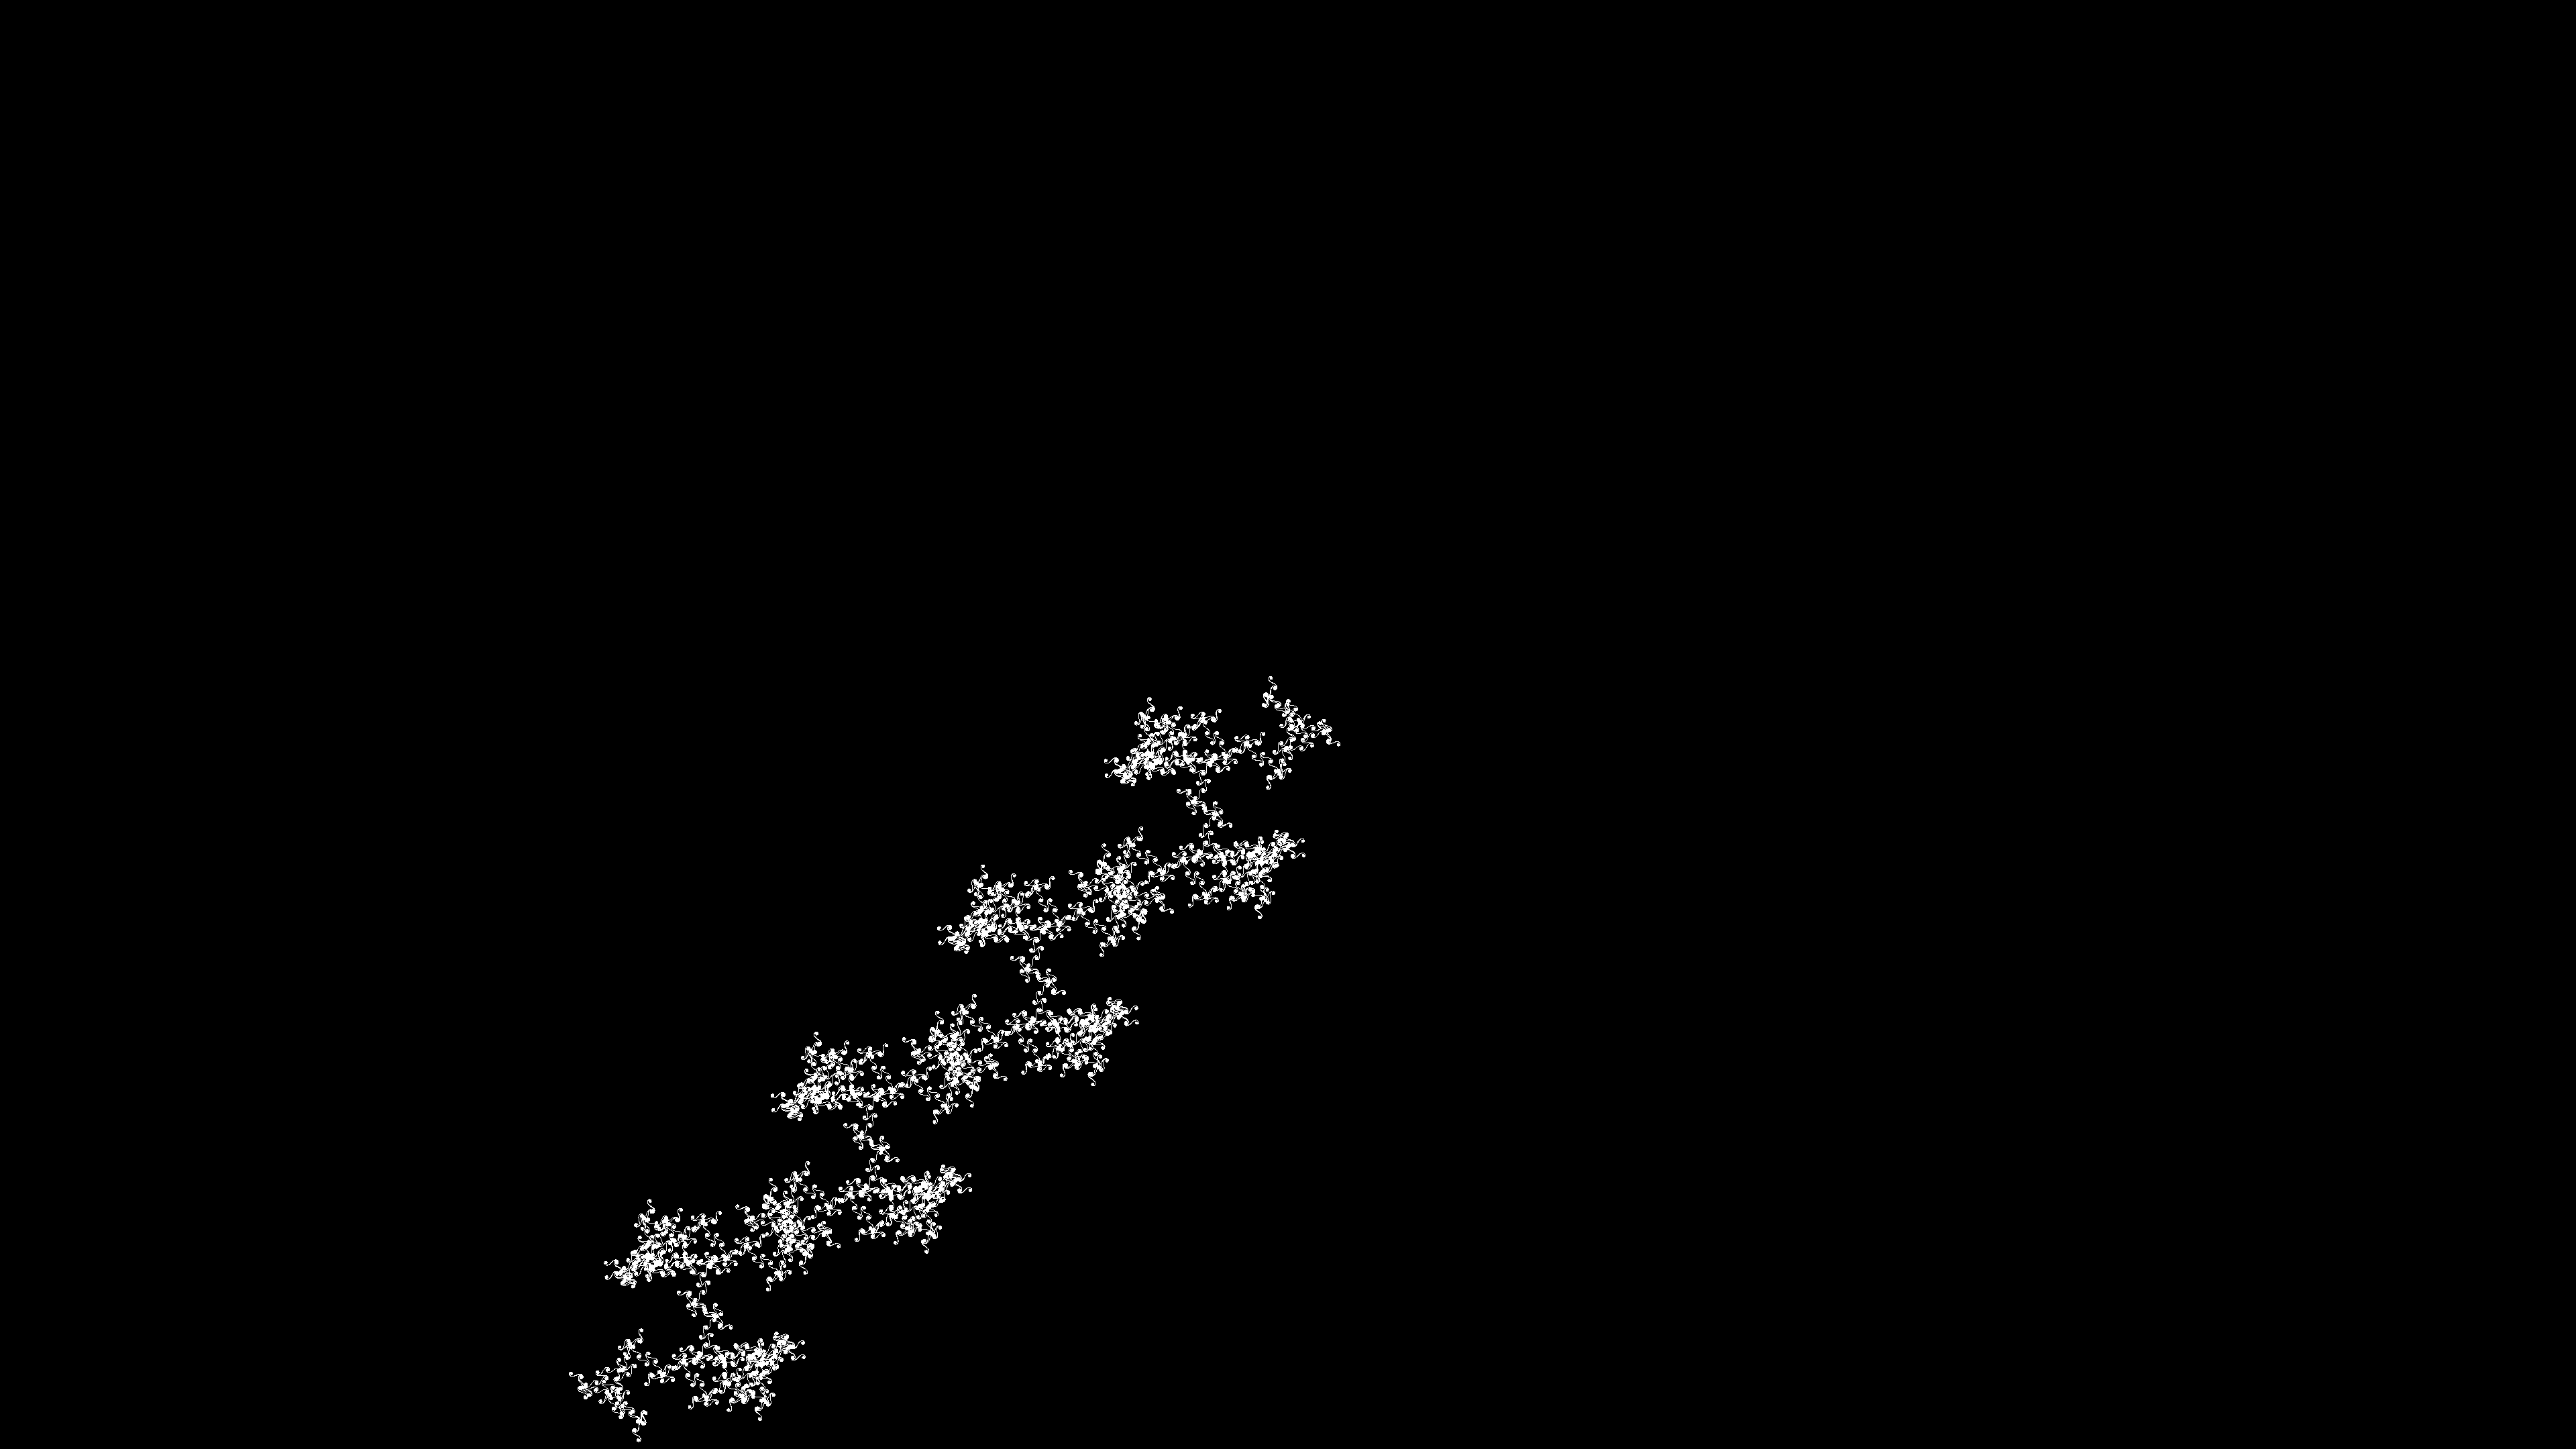
\includegraphics[width=\linewidth]{./stepsplusoneimages/0000000154.png}
    \caption{tf p=499 q=200251 theta=000 89707417.png}
  \end{subfigure}
  \caption{n=152 s=400 s+1=401}
  \label{fig:n=152}
\end{figure}
\begin{figure}[H]
  \centering
  \begin{subfigure}[t]{0.48\textwidth}
    \centering
    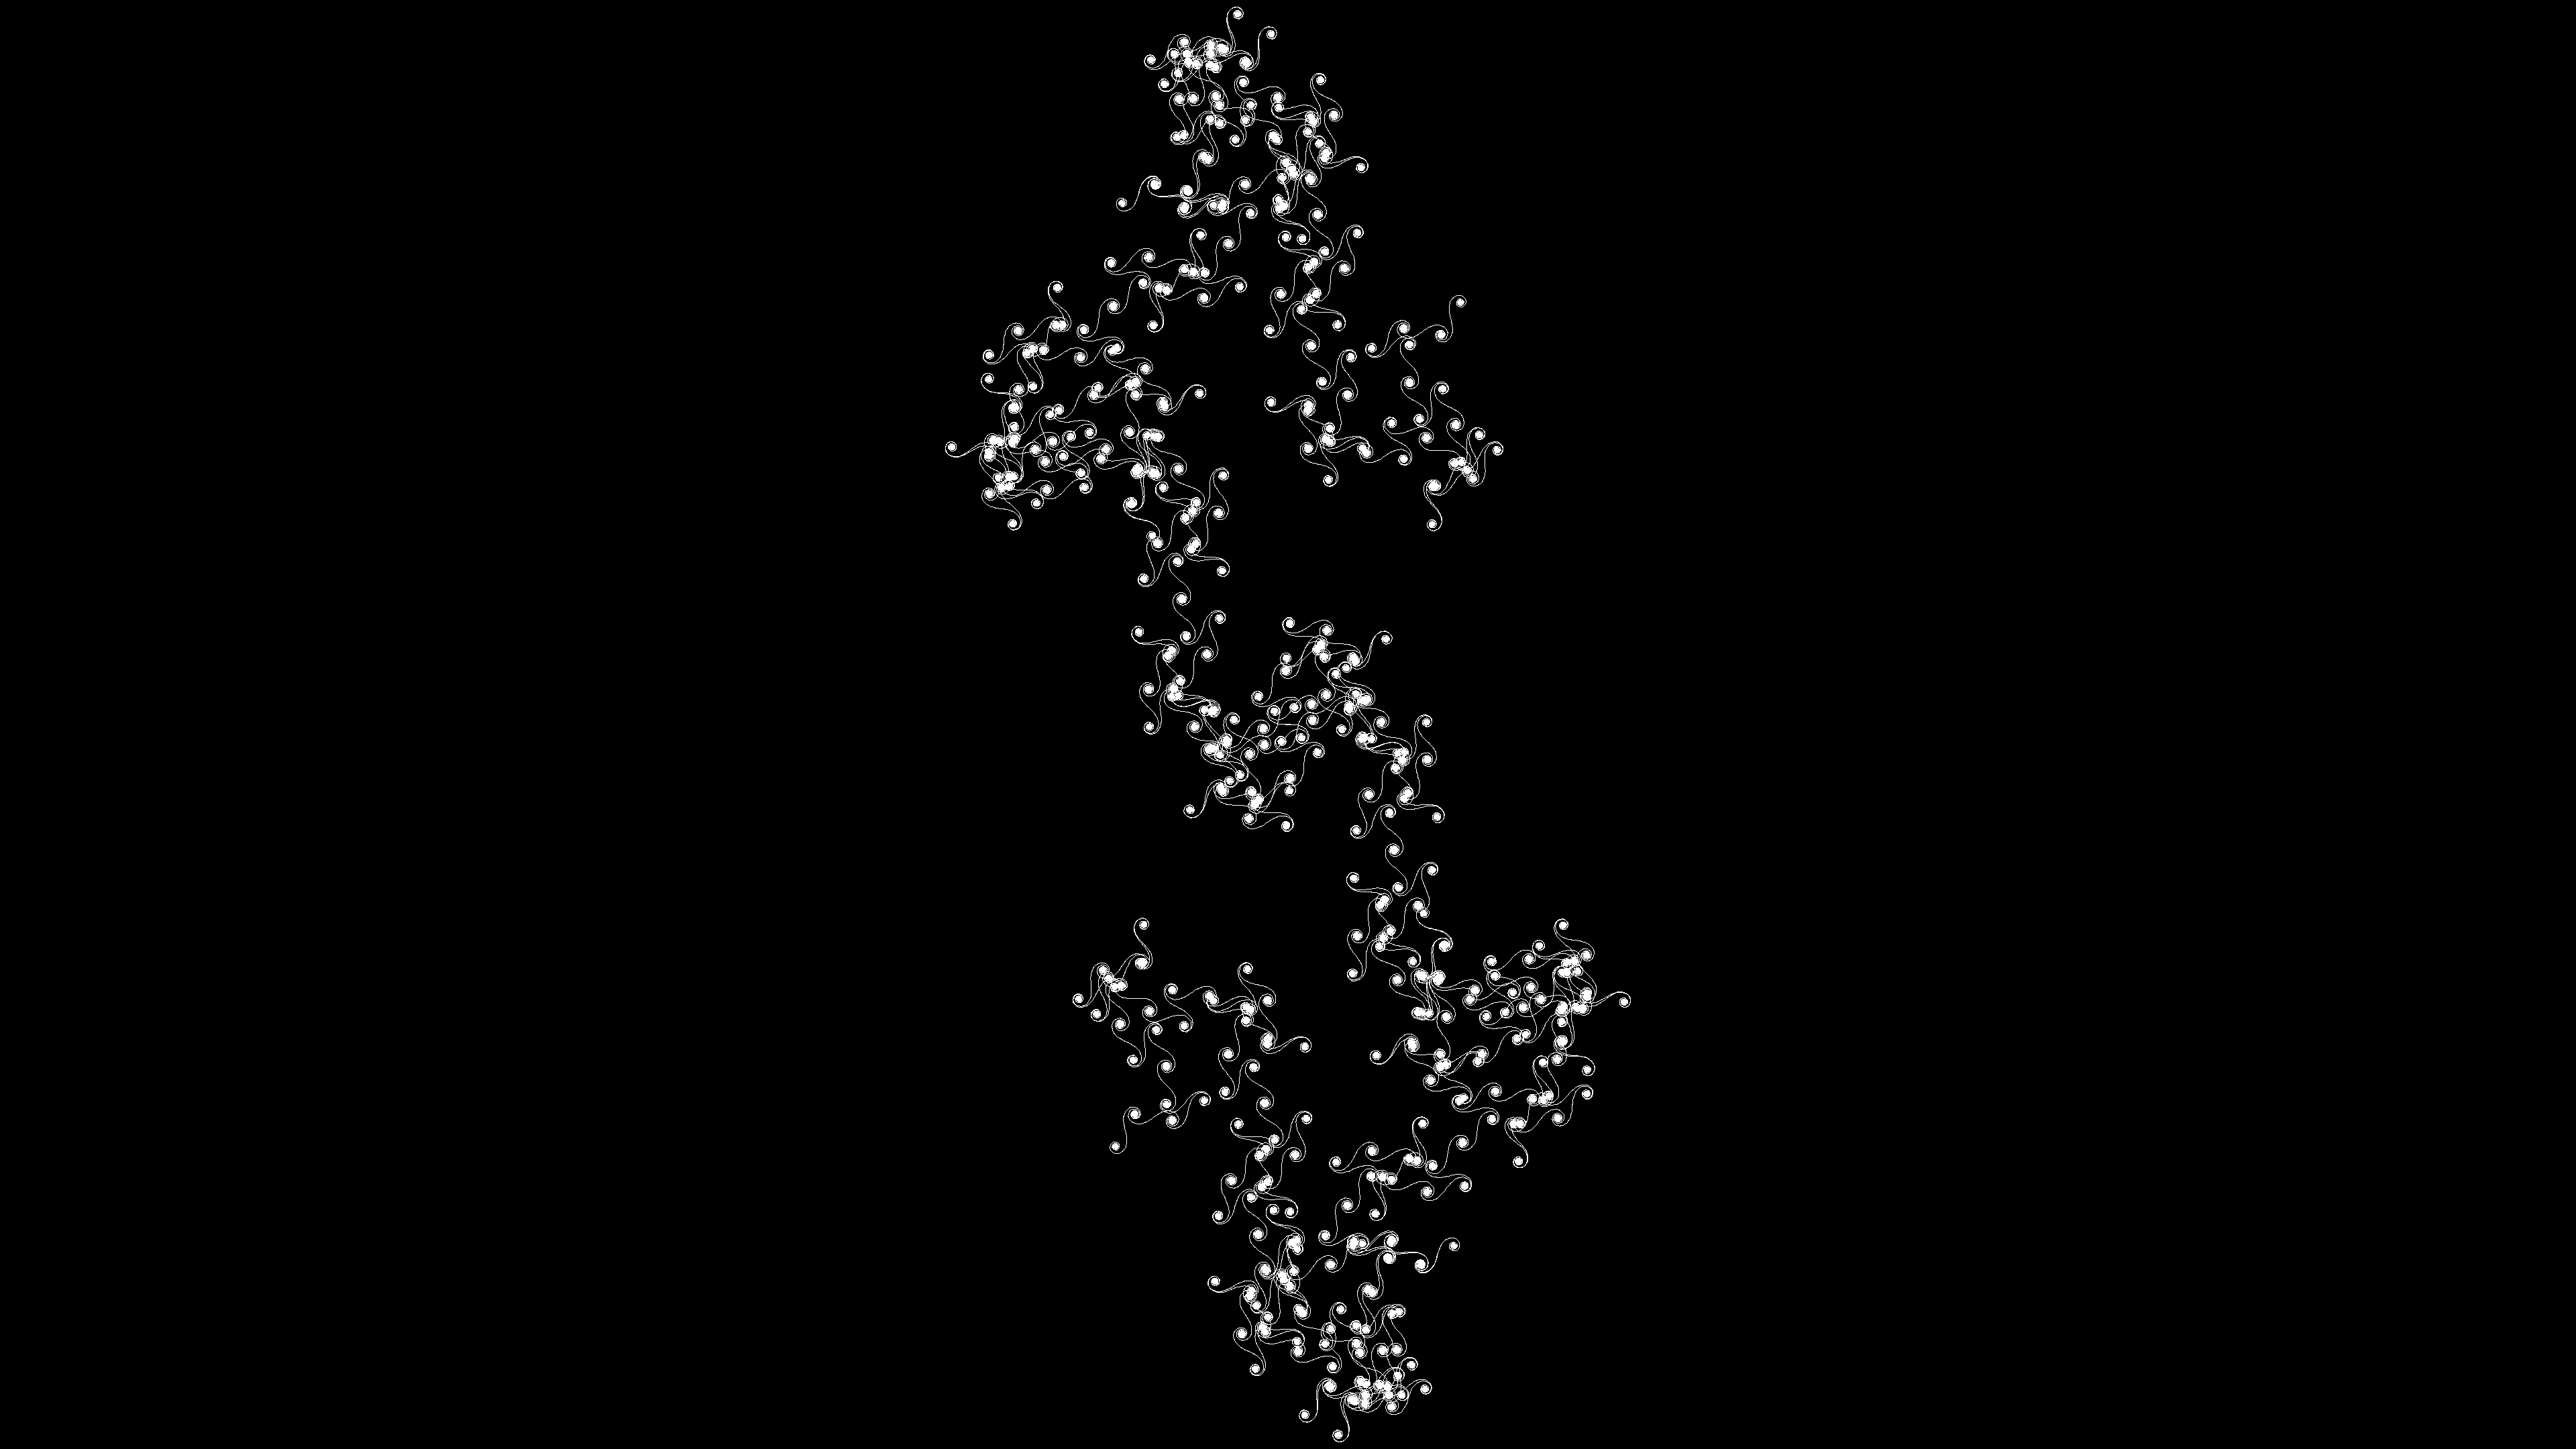
\includegraphics[width=\linewidth]{./stepsplusoneimages/0000000155.png}
    \caption{tf p=499 q=199754 theta=000 89930615.png}
  \end{subfigure}
  \begin{subfigure}[t]{0.48\textwidth}
    \centering
    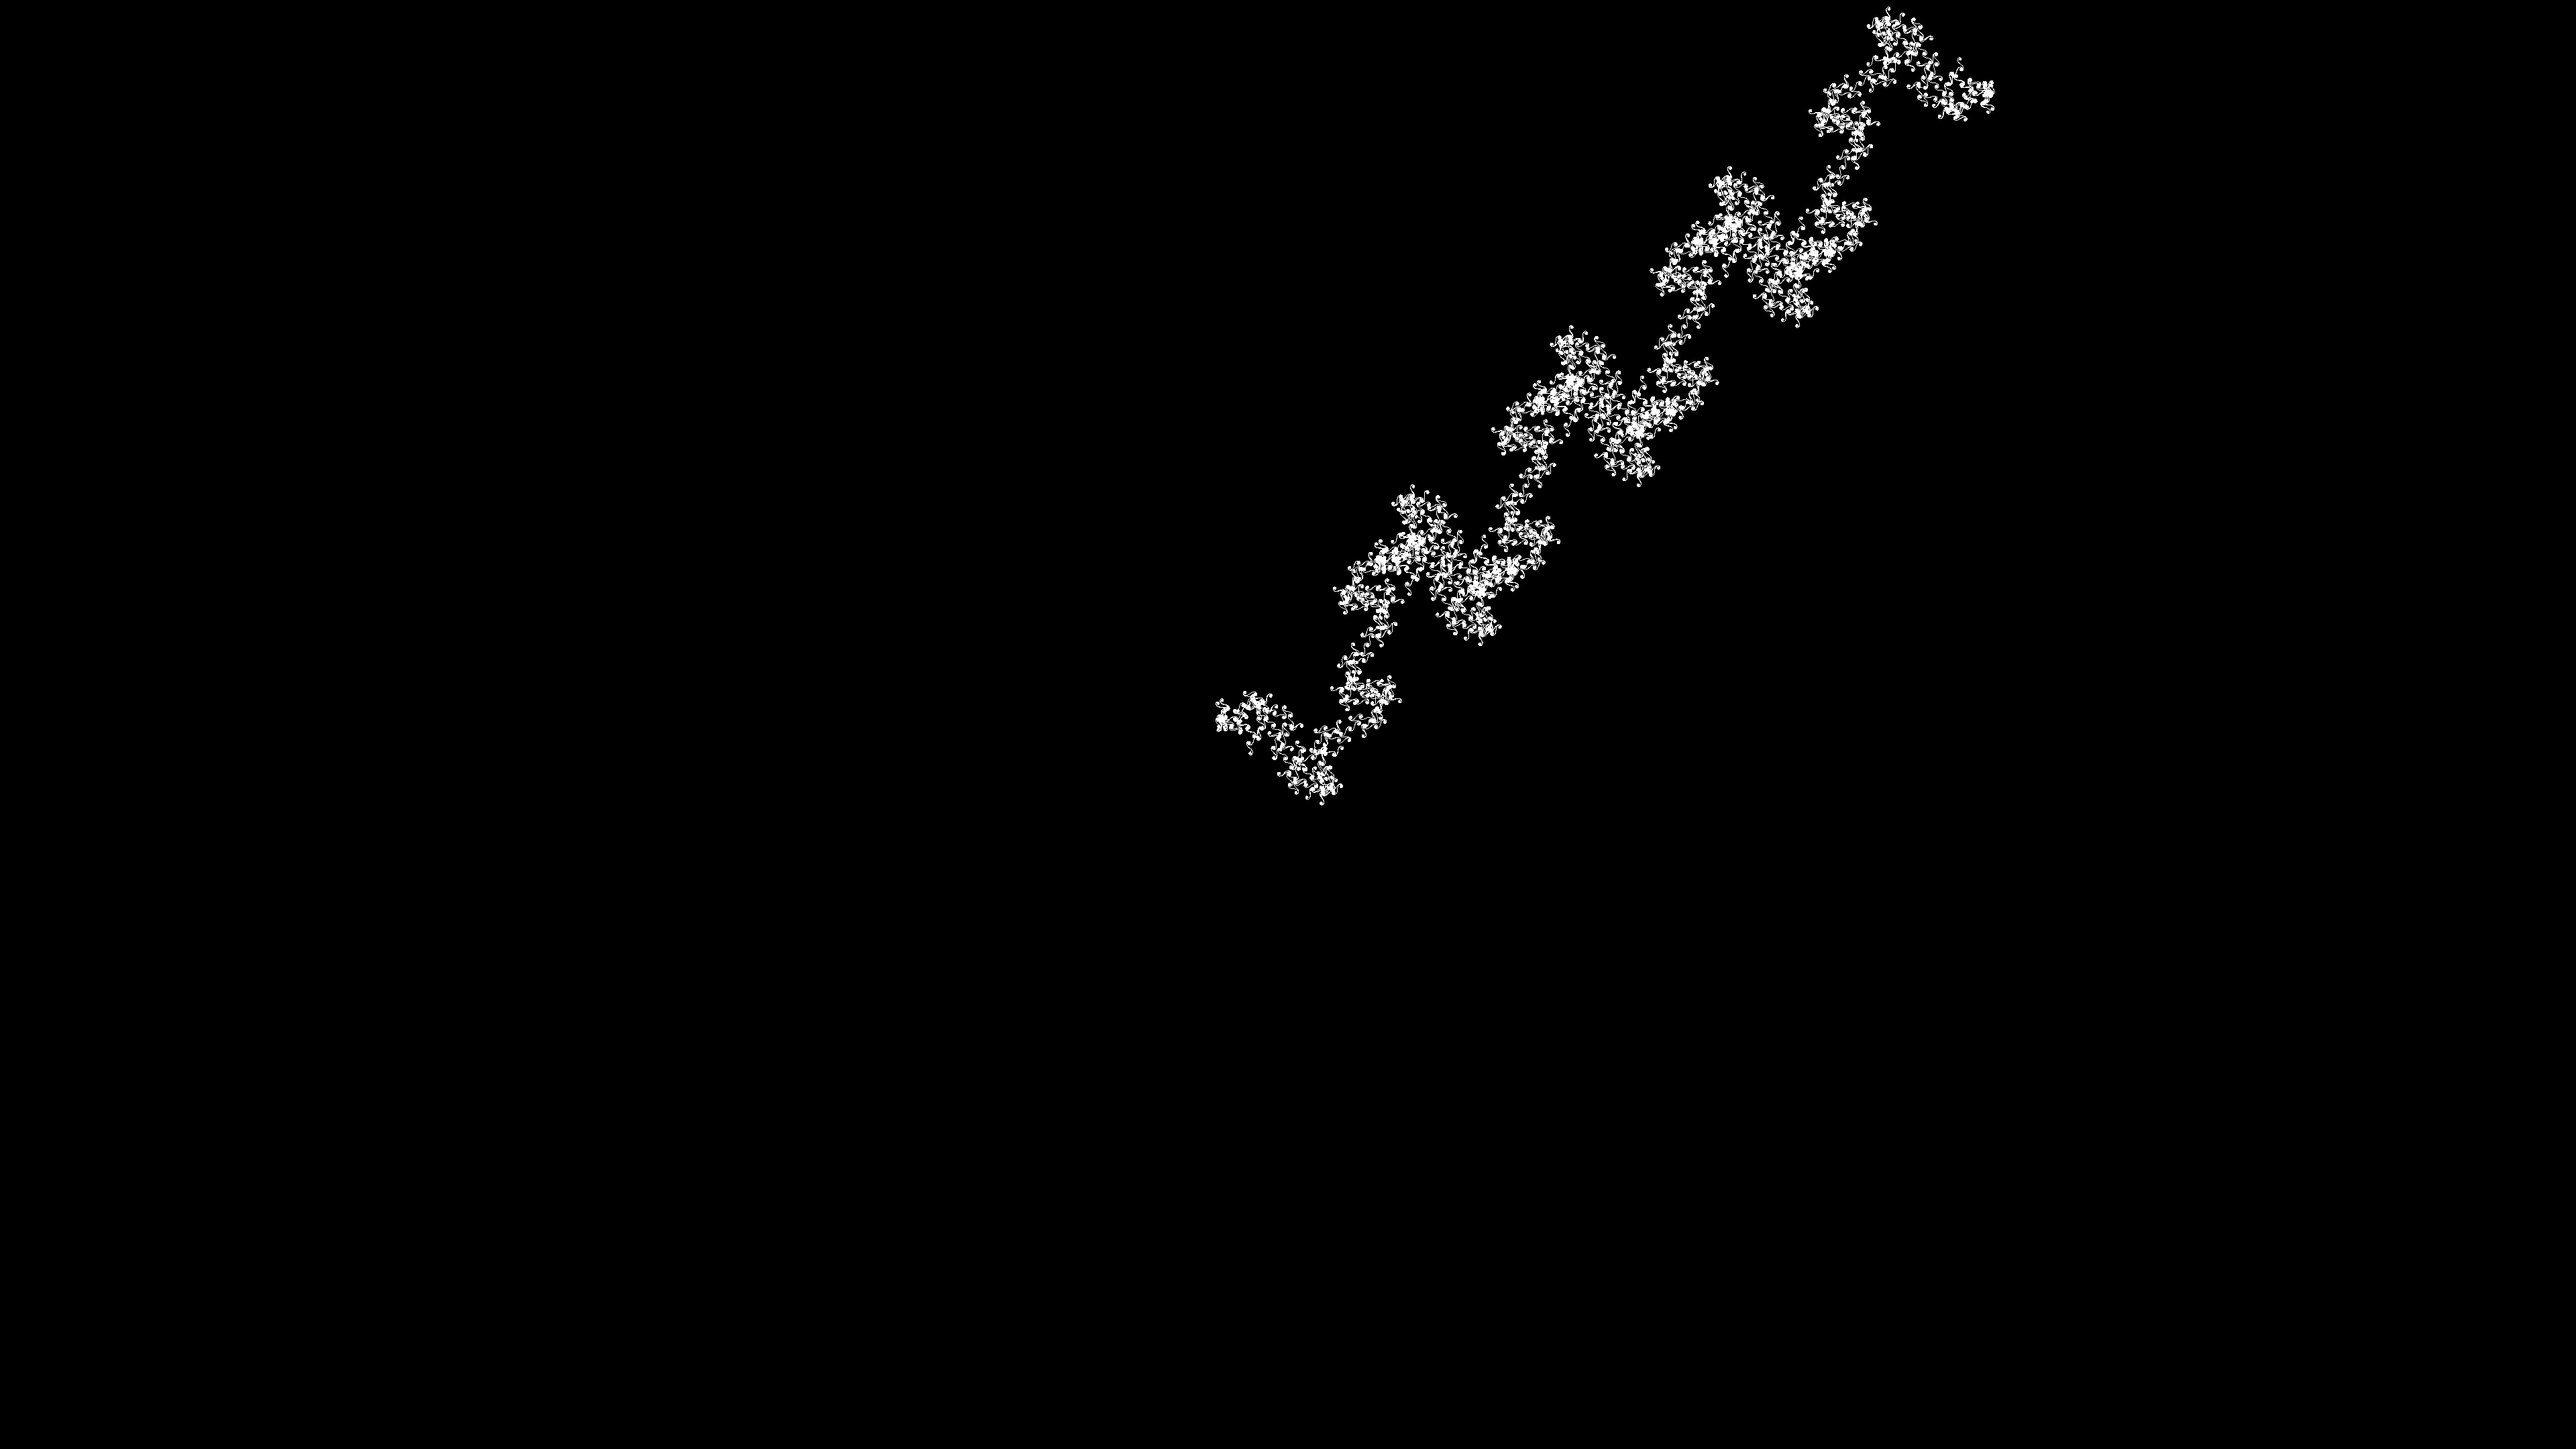
\includegraphics[width=\linewidth]{./stepsplusoneimages/0000000156.png}
    \caption{tf p=499 q=200253 theta=000 89706521.png}
  \end{subfigure}
  \caption{n=154 s=400 s+1=401}
  \label{fig:n=154}
\end{figure}
\begin{figure}[H]
  \centering
  \begin{subfigure}[t]{0.48\textwidth}
    \centering
    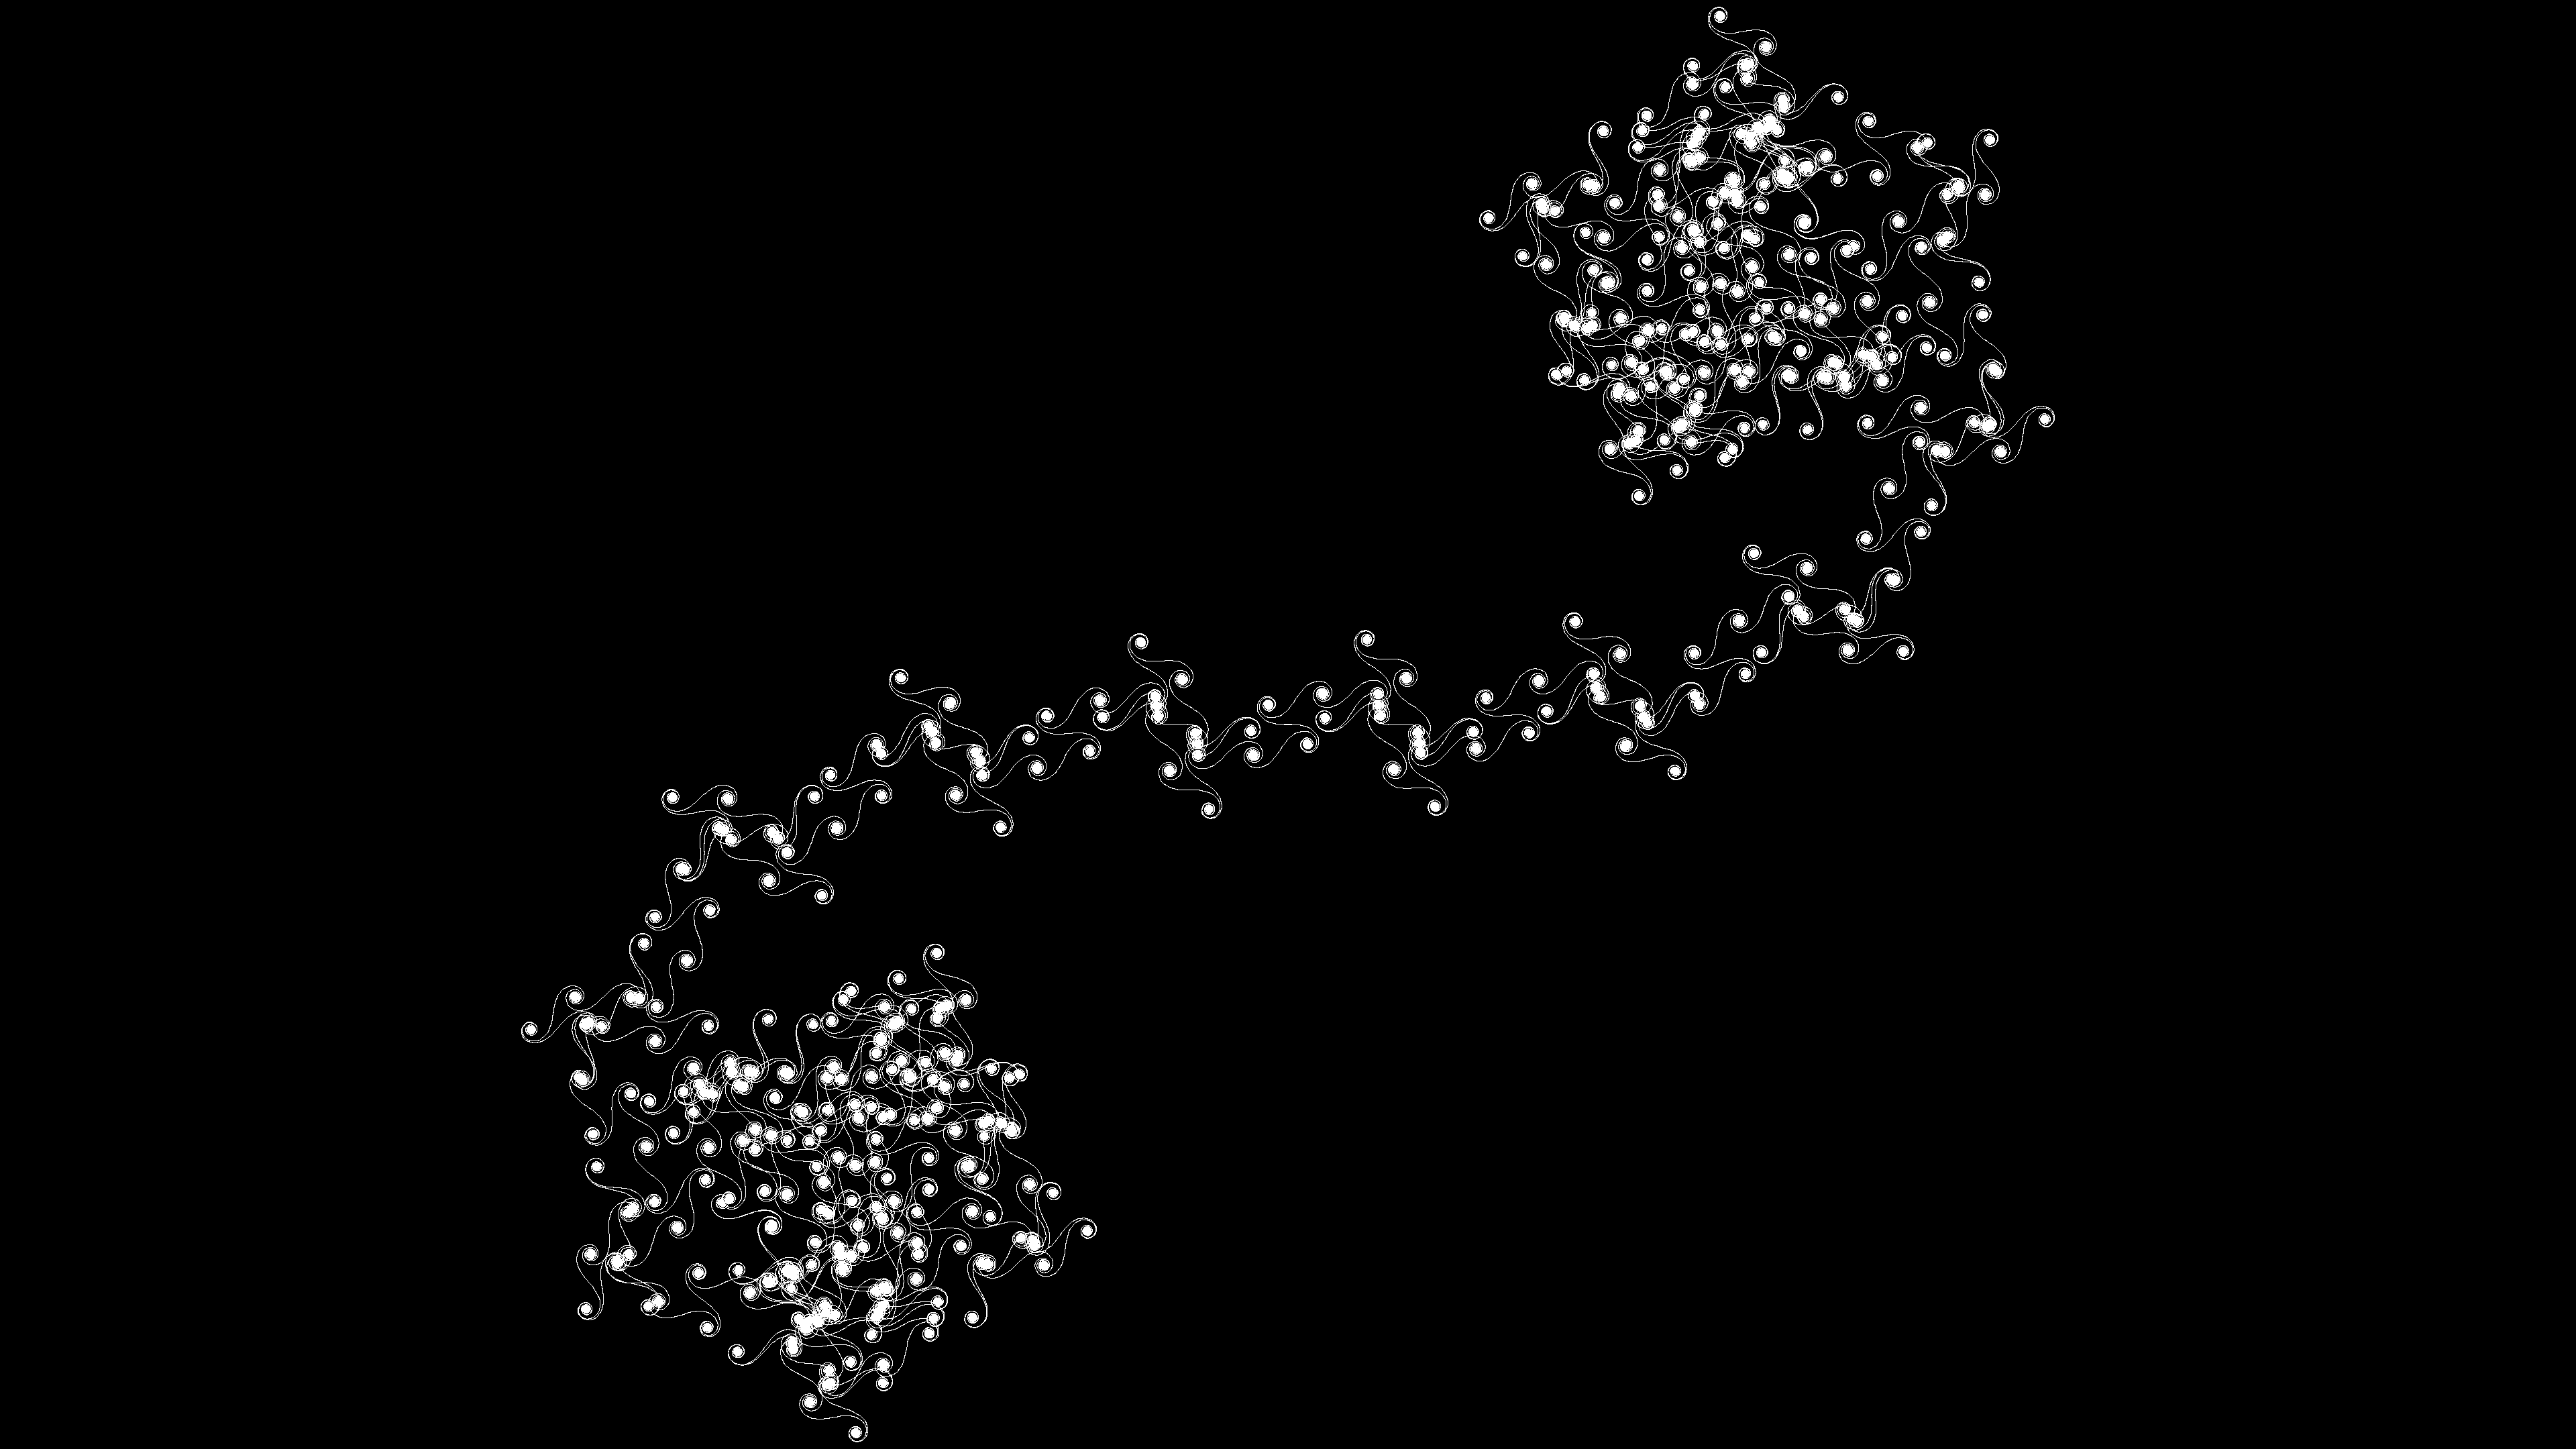
\includegraphics[width=\linewidth]{./stepsplusoneimages/0000000157.png}
    \caption{tf p=499 q=199756 theta=000 89929714.png}
  \end{subfigure}
  \begin{subfigure}[t]{0.48\textwidth}
    \centering
    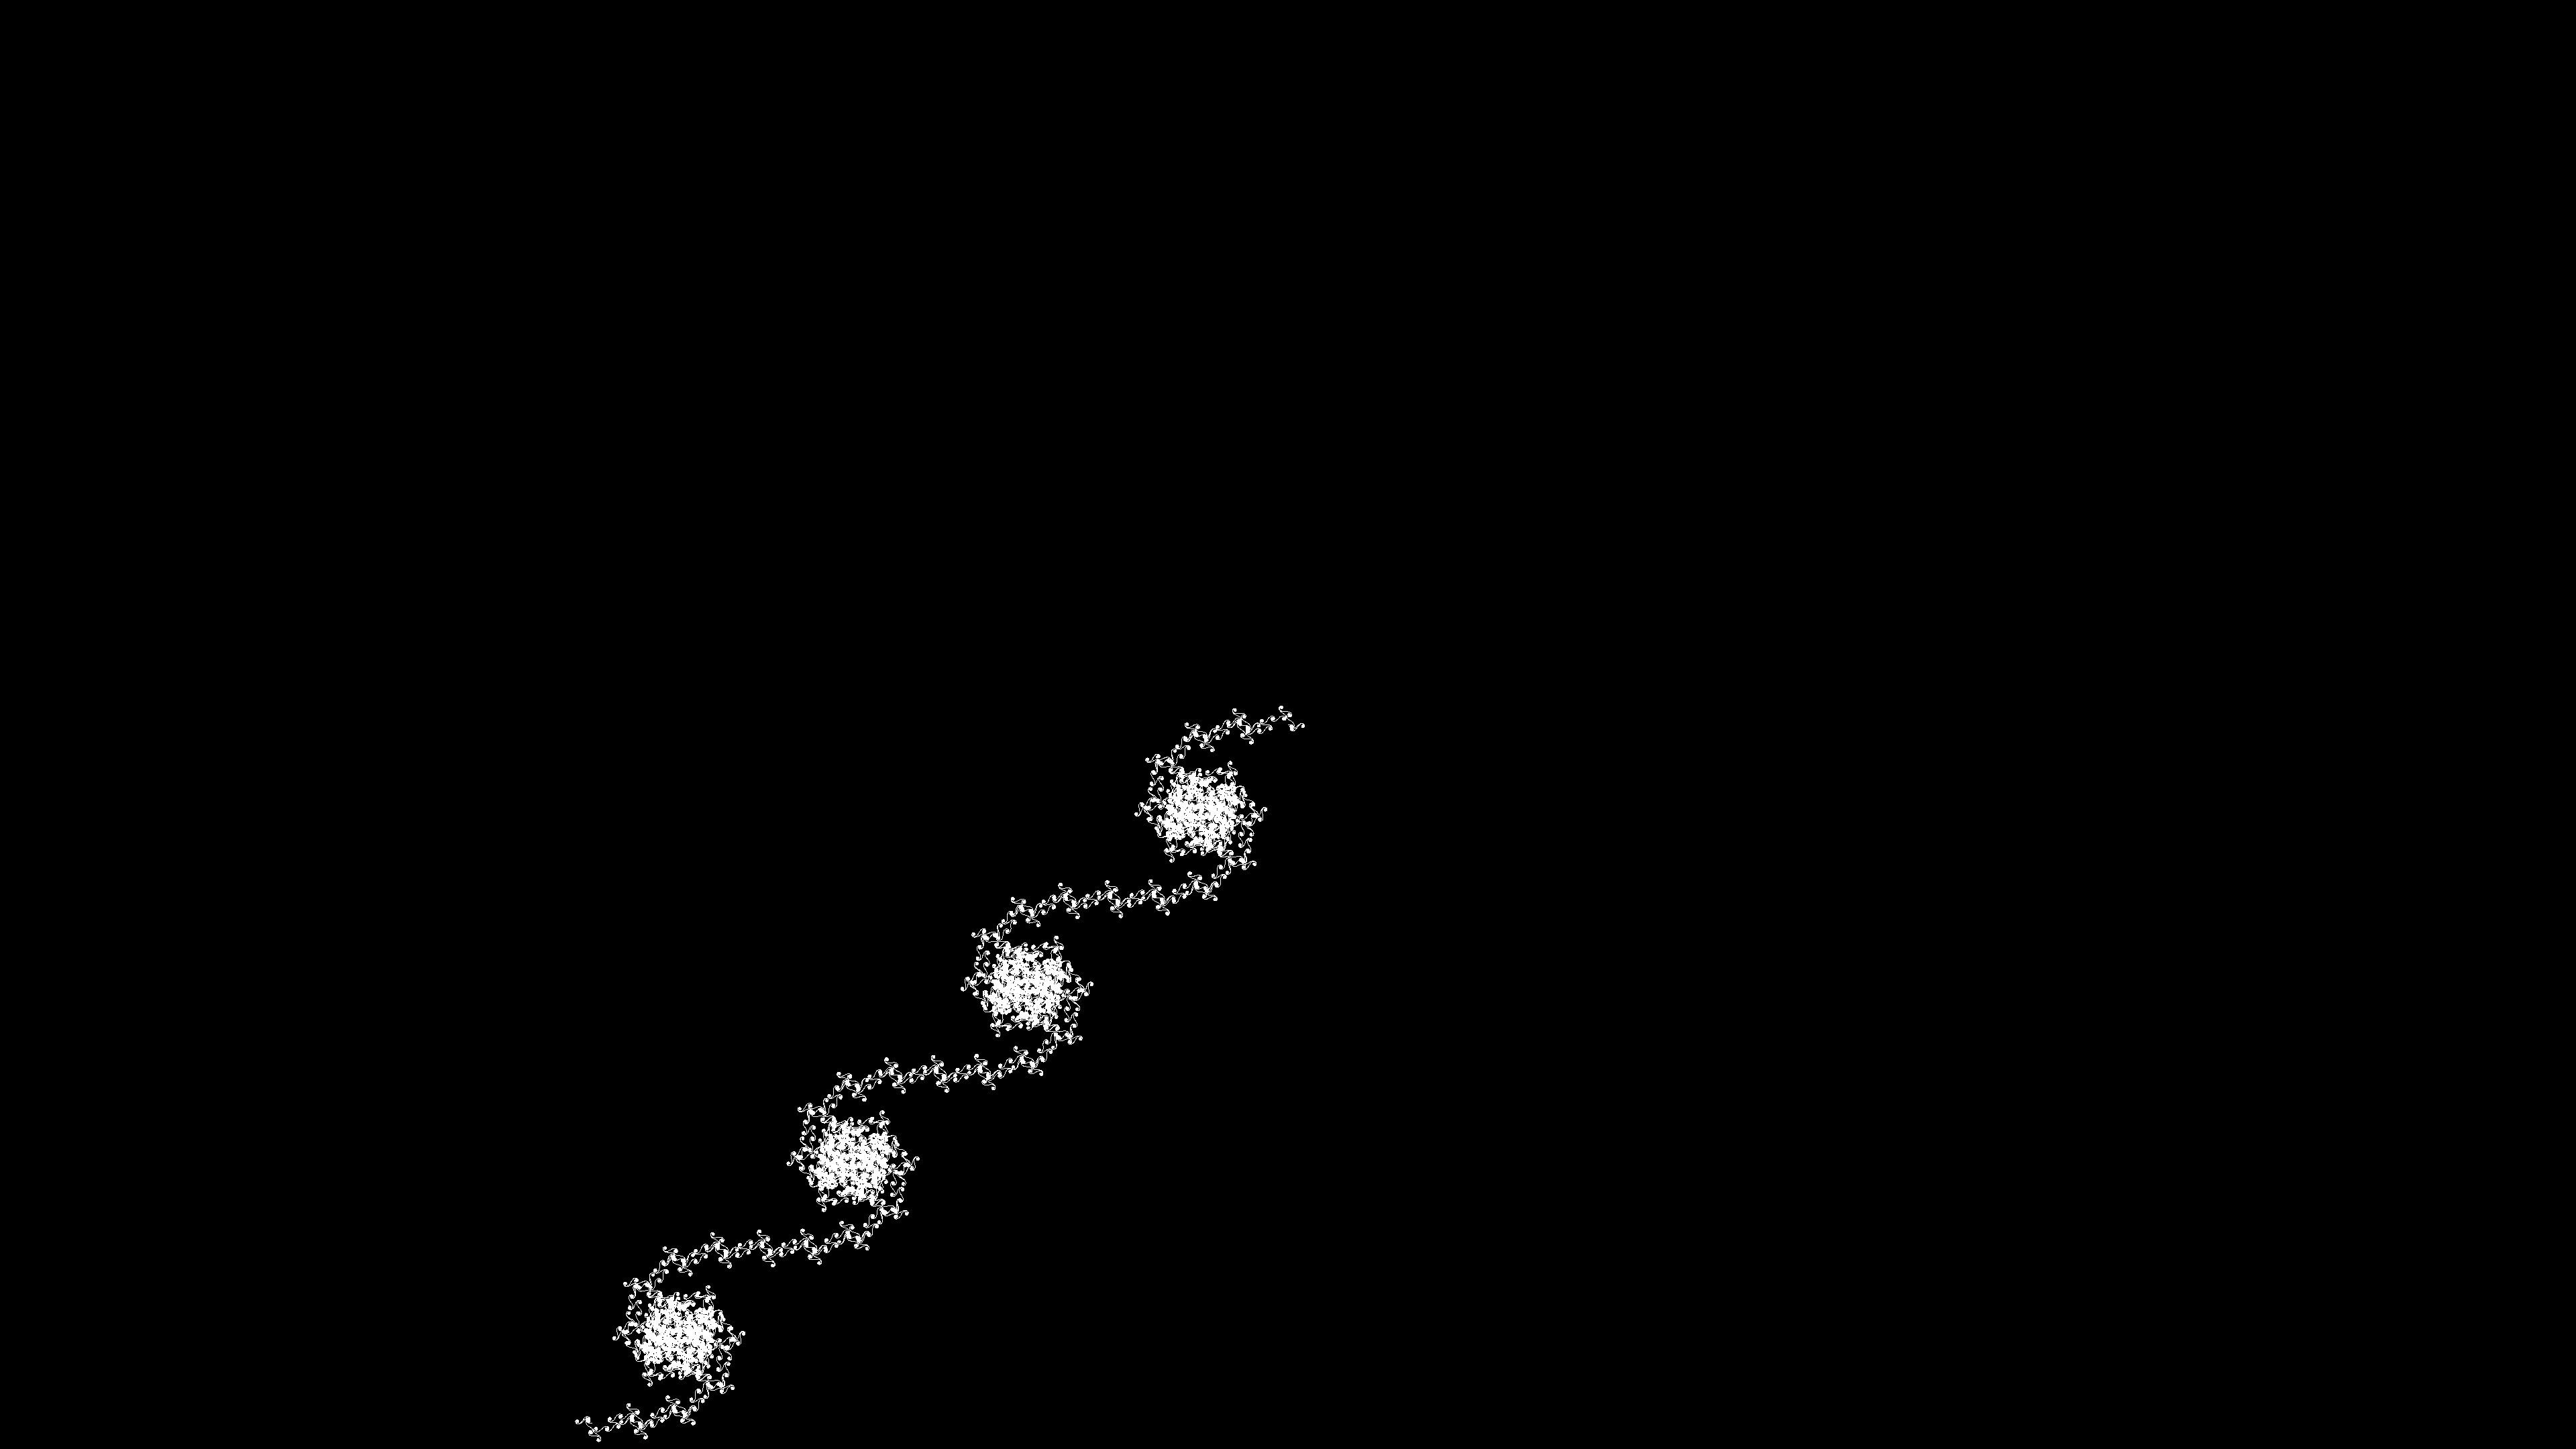
\includegraphics[width=\linewidth]{./stepsplusoneimages/0000000158.png}
    \caption{tf p=499 q=200255 theta=000 89705625.png}
  \end{subfigure}
  \caption{n=156 s=400 s+1=401}
  \label{fig:n=156}
\end{figure}
\begin{figure}[H]
  \centering
  \begin{subfigure}[t]{0.48\textwidth}
    \centering
    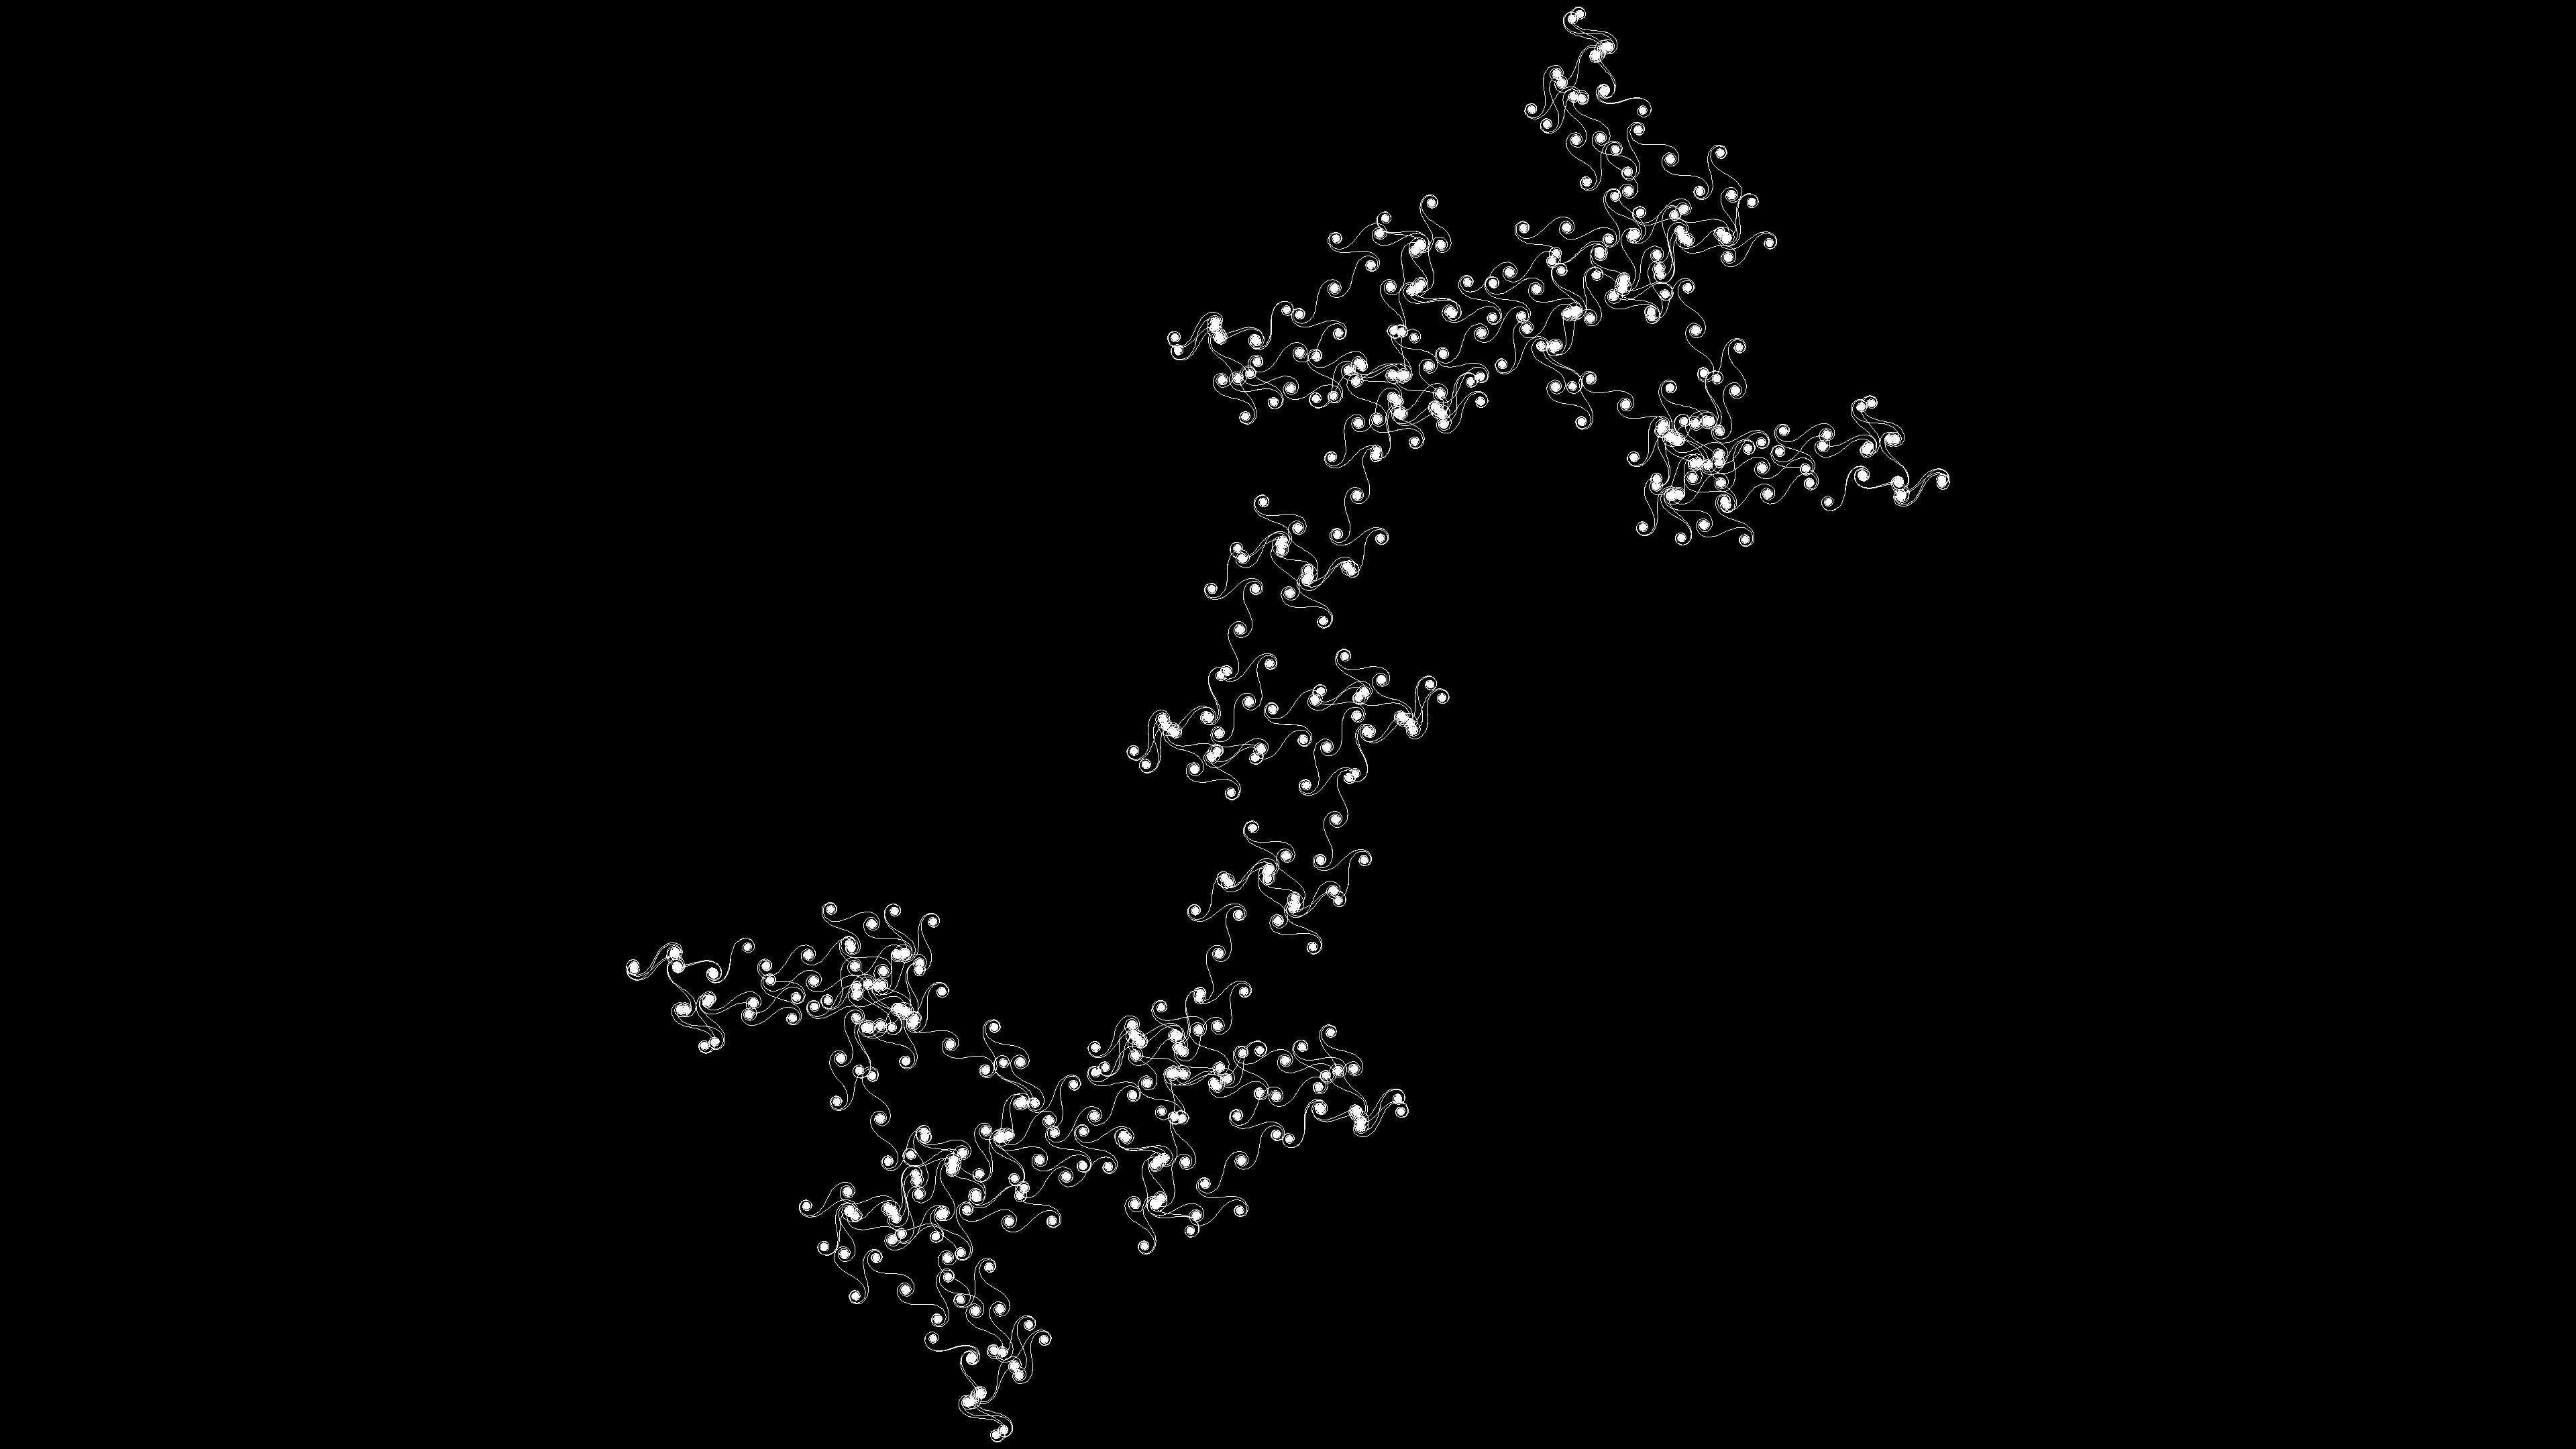
\includegraphics[width=\linewidth]{./stepsplusoneimages/0000000159.png}
    \caption{tf p=499 q=199758 theta=000 89928814.png}
  \end{subfigure}
  \begin{subfigure}[t]{0.48\textwidth}
    \centering
    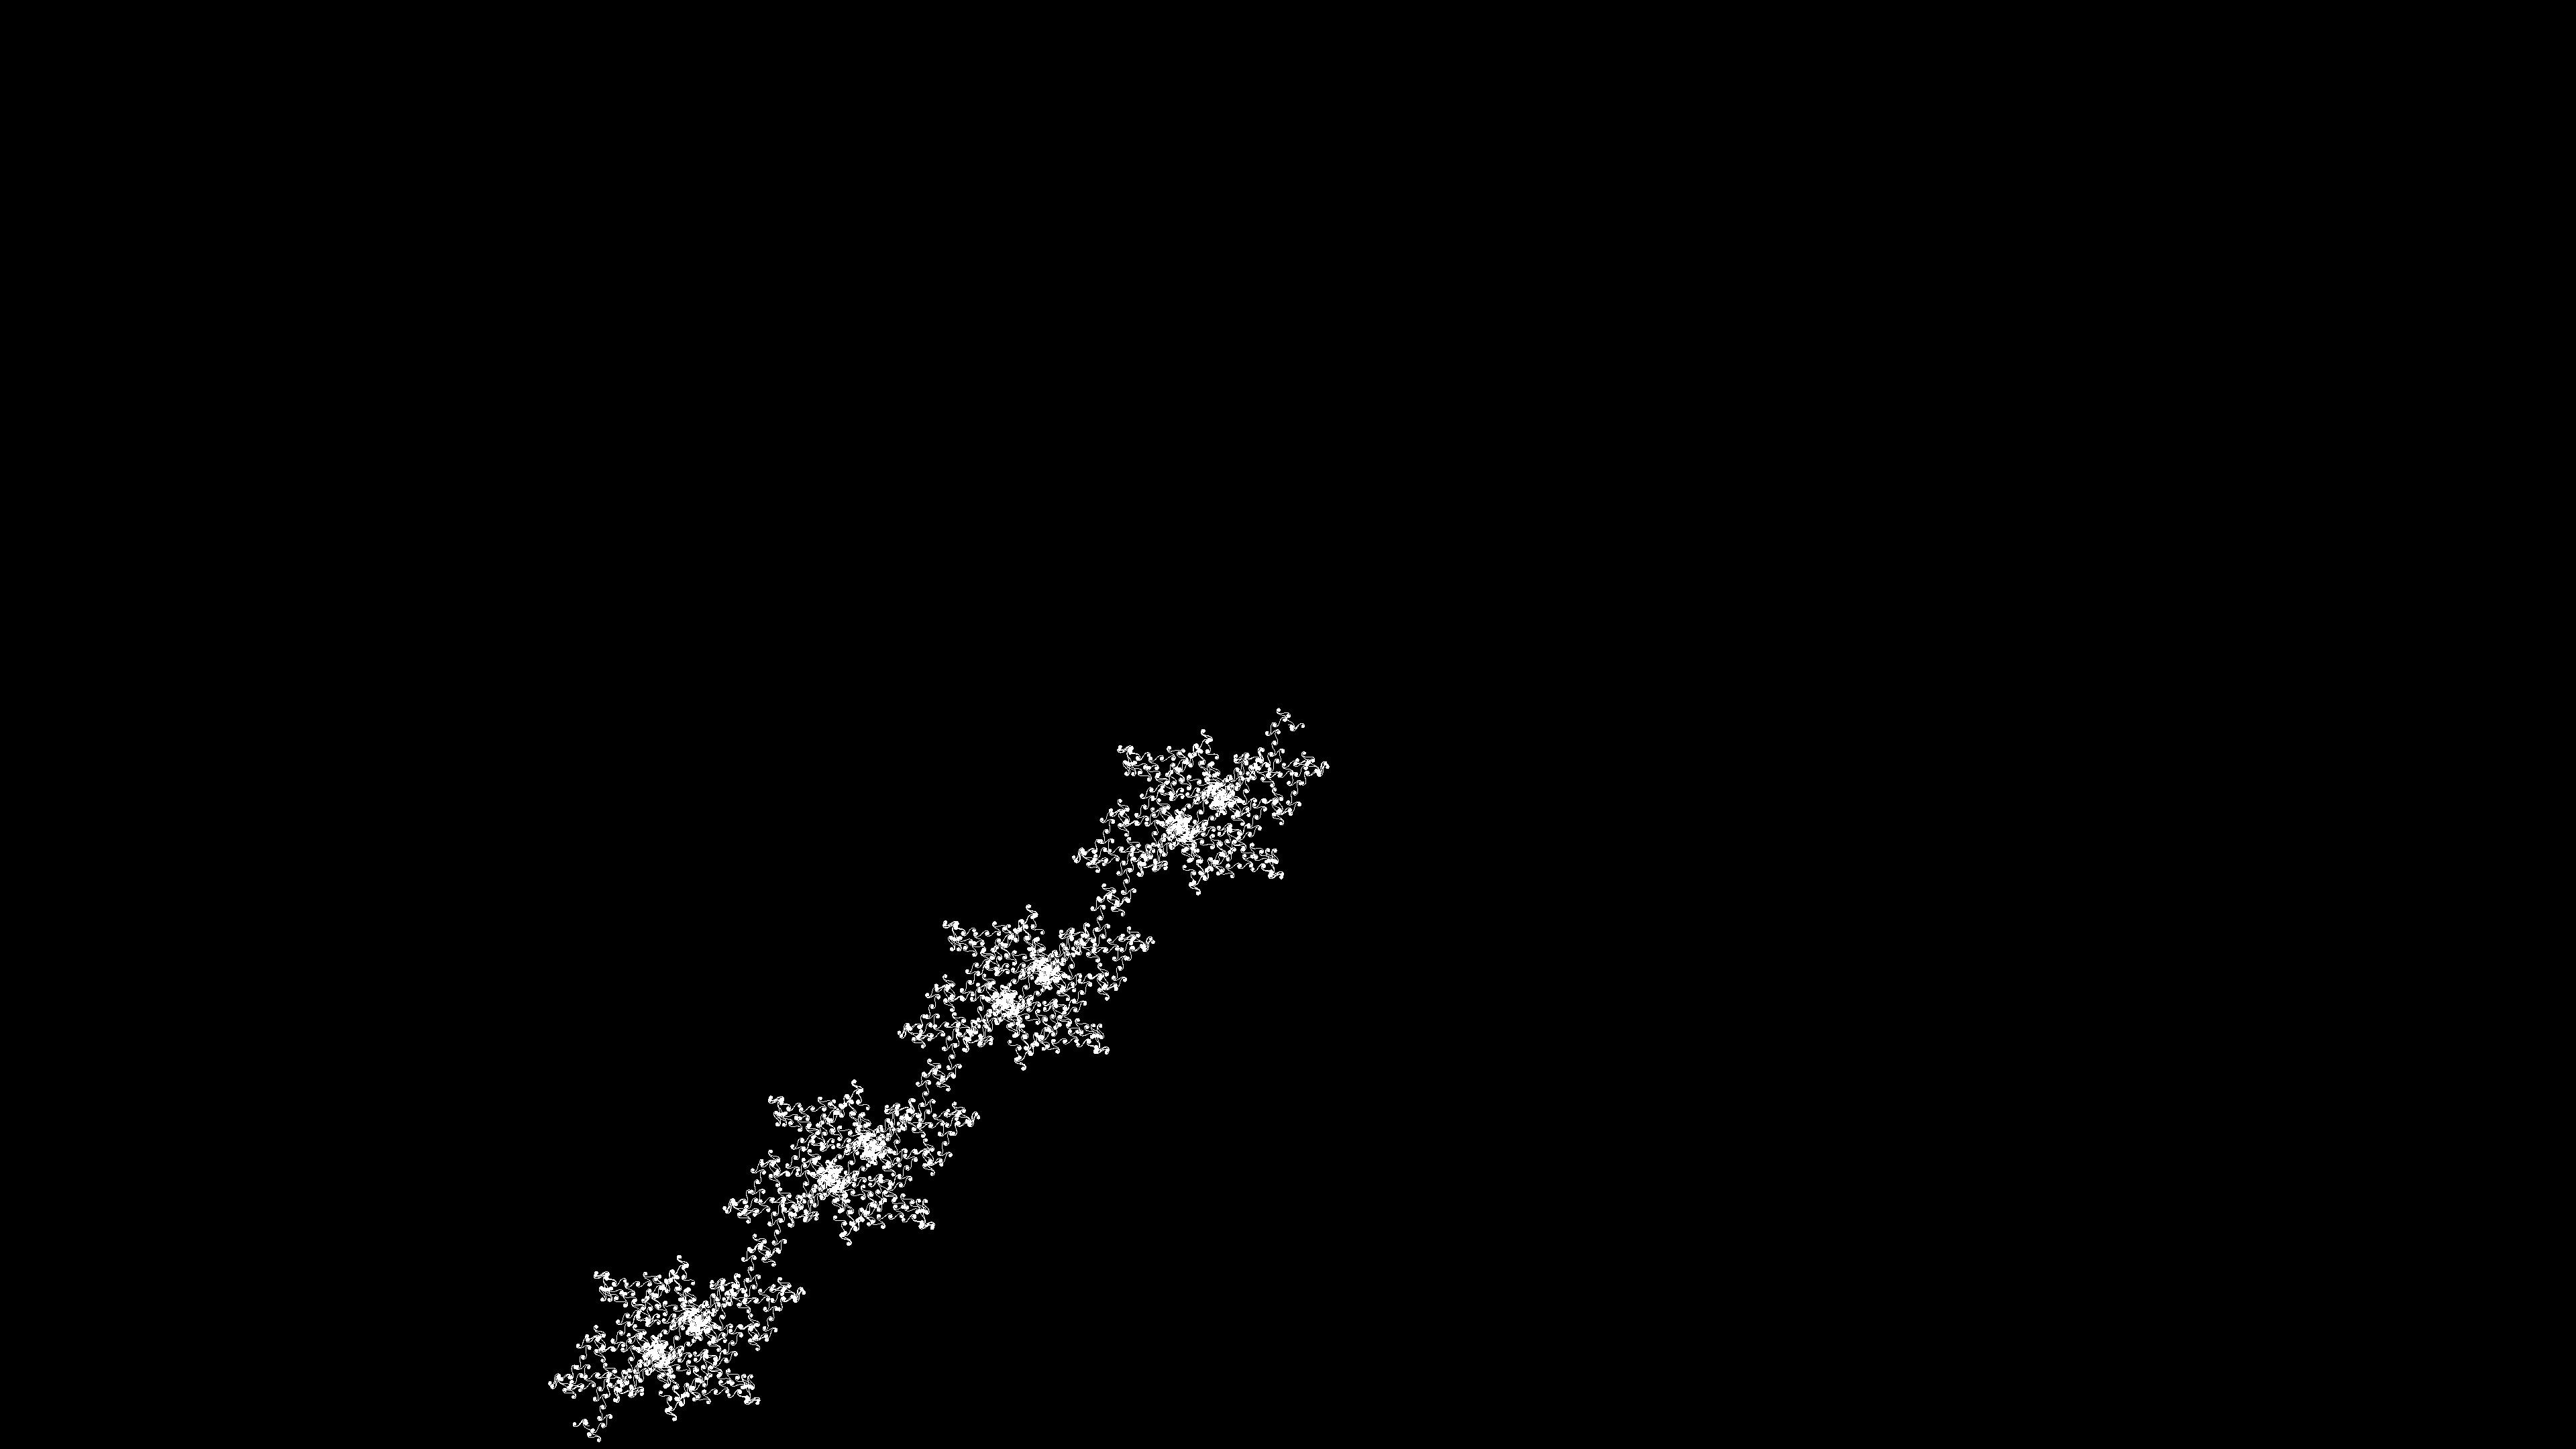
\includegraphics[width=\linewidth]{./stepsplusoneimages/0000000160.png}
    \caption{tf p=499 q=200257 theta=000 89704729.png}
  \end{subfigure}
  \caption{n=158 s=400 s+1=401}
  \label{fig:n=158}
\end{figure}
\begin{figure}[H]
  \centering
  \begin{subfigure}[t]{0.48\textwidth}
    \centering
    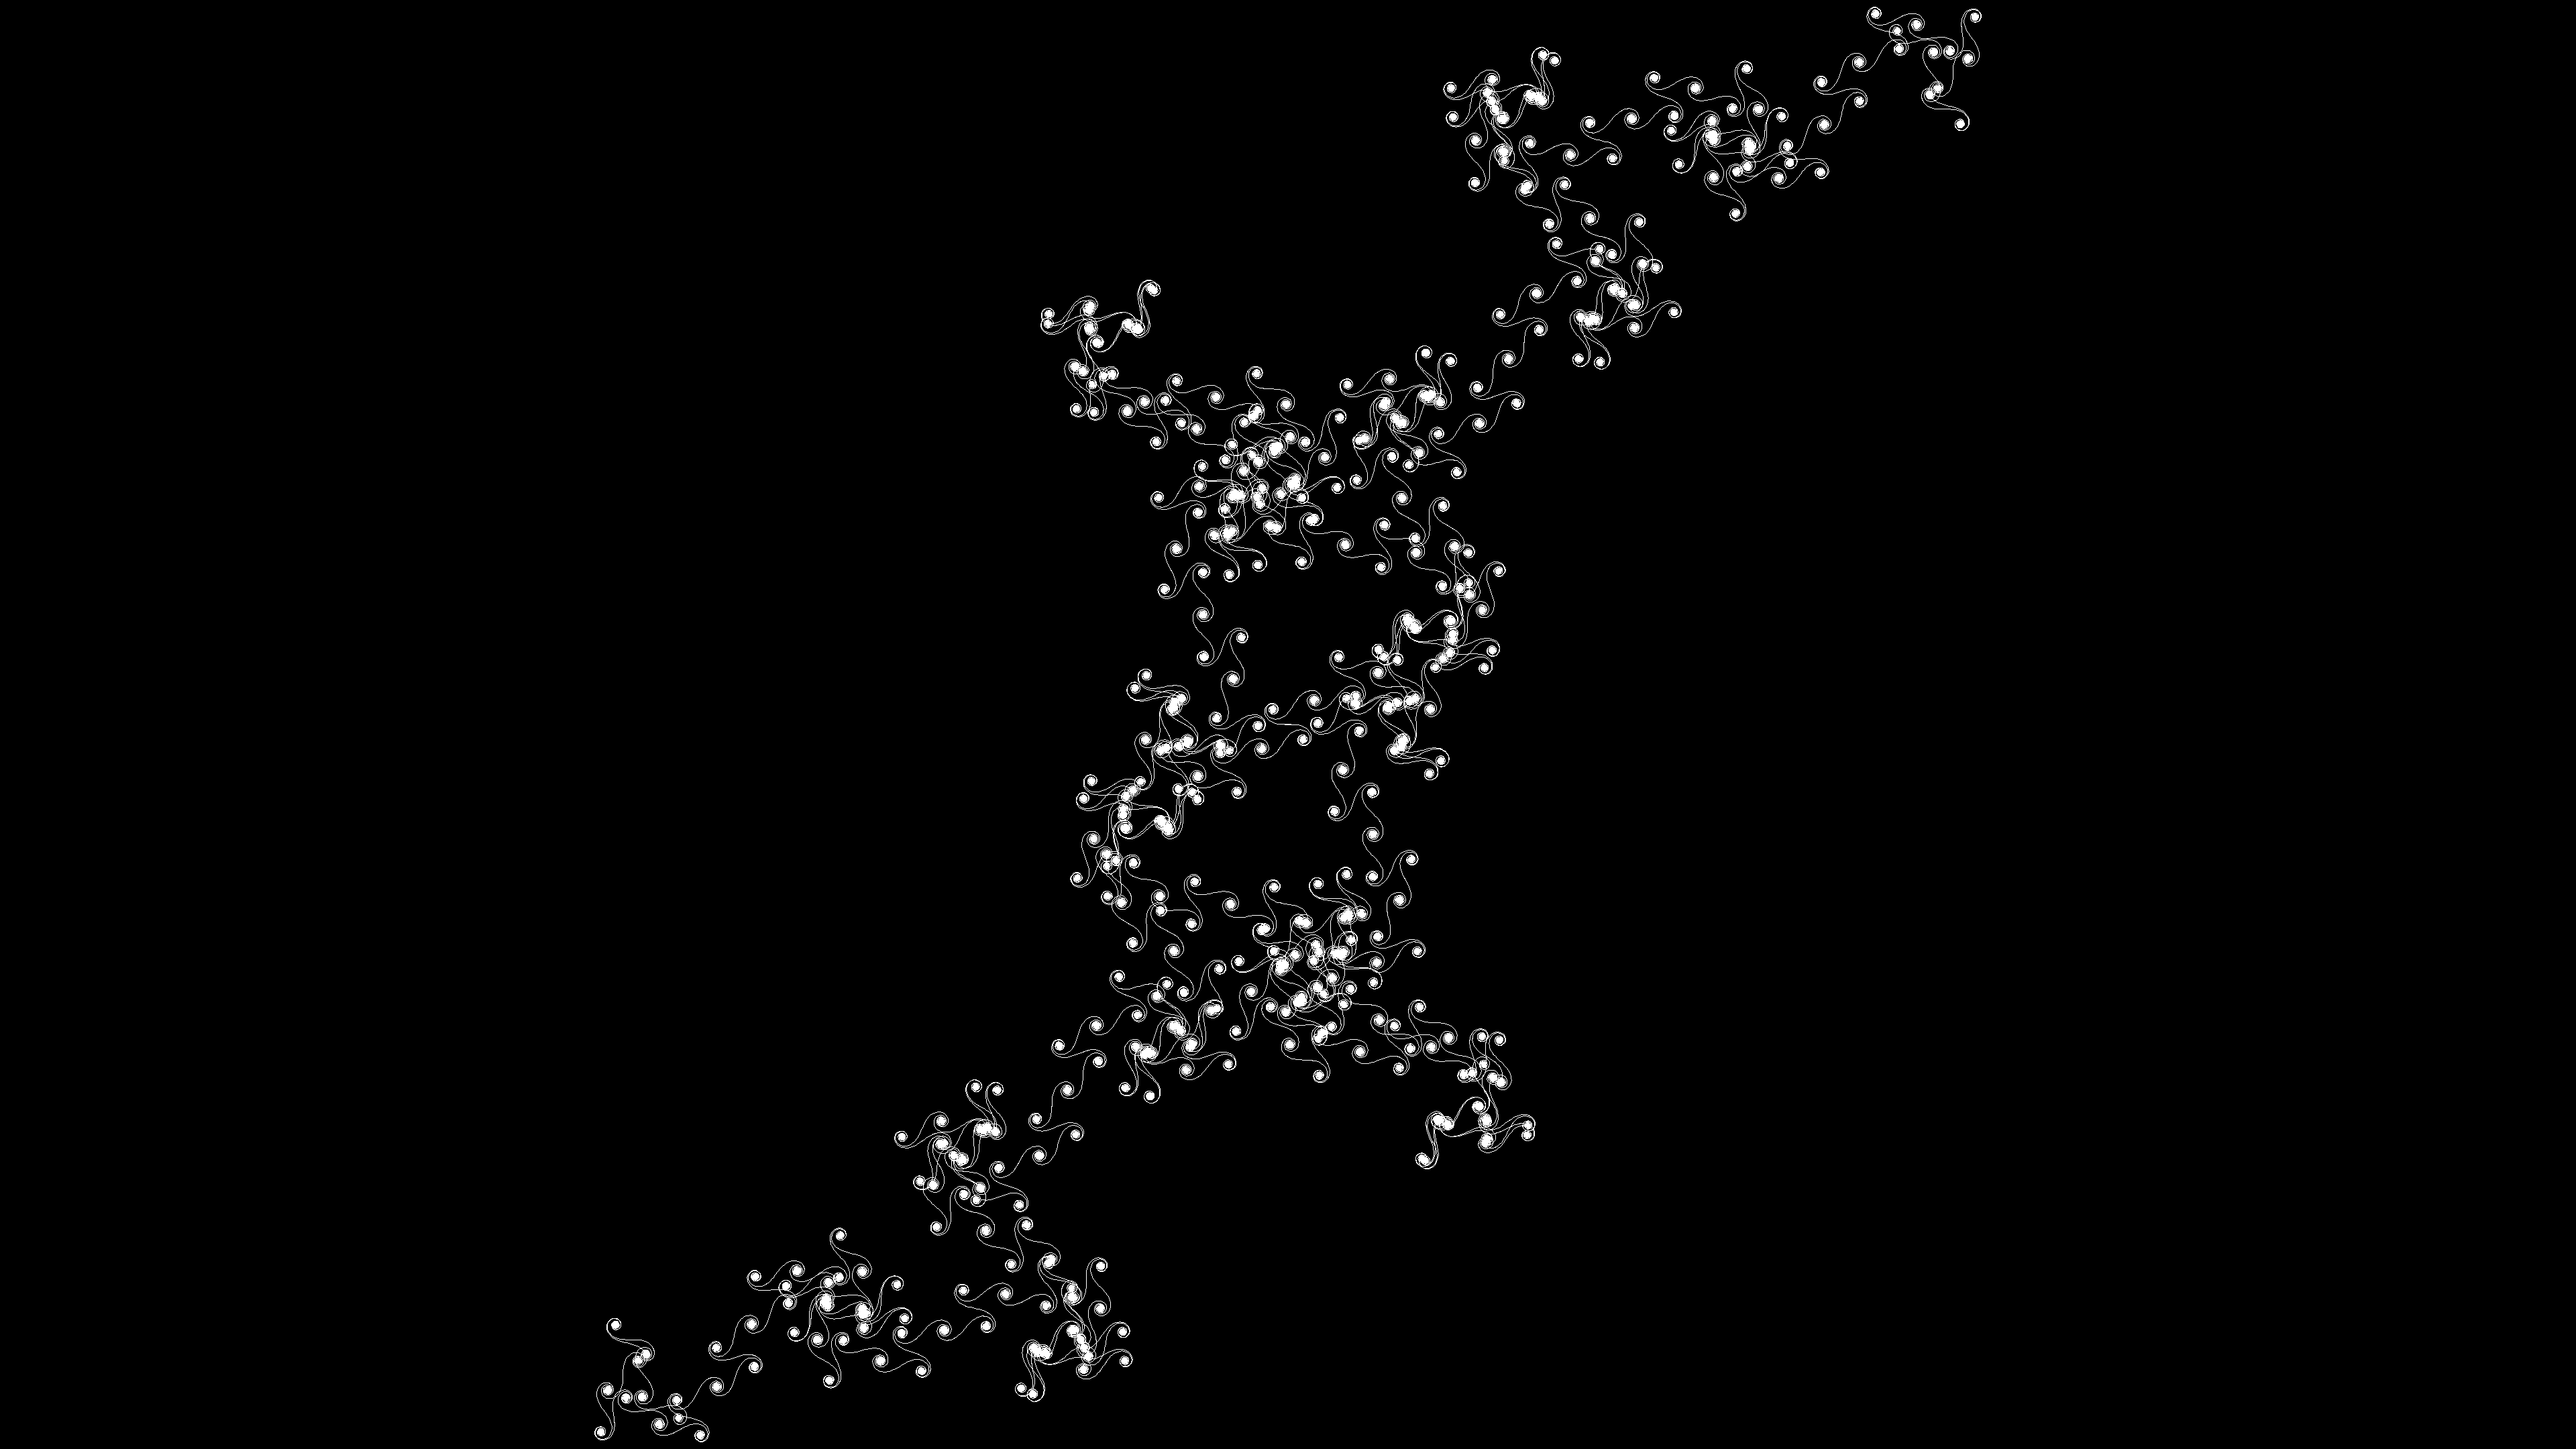
\includegraphics[width=\linewidth]{./stepsplusoneimages/0000000161.png}
    \caption{tf p=499 q=199760 theta=000 89927913.png}
  \end{subfigure}
  \begin{subfigure}[t]{0.48\textwidth}
    \centering
    \includegraphics[width=\linewidth]{./stepsplusoneimages/0000000162.png}
    \caption{tf p=499 q=200259 theta=000 89703834.png}
  \end{subfigure}
  \caption{n=160 s=400 s+1=401}
  \label{fig:n=160}
\end{figure}
\begin{figure}[H]
  \centering
  \begin{subfigure}[t]{0.48\textwidth}
    \centering
    \includegraphics[width=\linewidth]{./stepsplusoneimages/0000000163.png}
    \caption{tf p=499 q=199762 theta=000 89927013.png}
  \end{subfigure}
  \begin{subfigure}[t]{0.48\textwidth}
    \centering
    \includegraphics[width=\linewidth]{./stepsplusoneimages/0000000164.png}
    \caption{tf p=499 q=200261 theta=000 89702938.png}
  \end{subfigure}
  \caption{n=162 s=400 s+1=401}
  \label{fig:n=162}
\end{figure}
\begin{figure}[H]
  \centering
  \begin{subfigure}[t]{0.48\textwidth}
    \centering
    \includegraphics[width=\linewidth]{./stepsplusoneimages/0000000165.png}
    \caption{tf p=499 q=199764 theta=000 89926113.png}
  \end{subfigure}
  \begin{subfigure}[t]{0.48\textwidth}
    \centering
    \includegraphics[width=\linewidth]{./stepsplusoneimages/0000000166.png}
    \caption{tf p=499 q=200263 theta=000 89702042.png}
  \end{subfigure}
  \caption{n=164 s=400 s+1=401}
  \label{fig:n=164}
\end{figure}
\begin{figure}[H]
  \centering
  \begin{subfigure}[t]{0.48\textwidth}
    \centering
    \includegraphics[width=\linewidth]{./stepsplusoneimages/0000000167.png}
    \caption{tf p=499 q=199766 theta=000 89925212.png}
  \end{subfigure}
  \begin{subfigure}[t]{0.48\textwidth}
    \centering
    \includegraphics[width=\linewidth]{./stepsplusoneimages/0000000168.png}
    \caption{tf p=499 q=200265 theta=000 89701146.png}
  \end{subfigure}
  \caption{n=166 s=400 s+1=401}
  \label{fig:n=166}
\end{figure}
\begin{figure}[H]
  \centering
  \begin{subfigure}[t]{0.48\textwidth}
    \centering
    \includegraphics[width=\linewidth]{./stepsplusoneimages/0000000169.png}
    \caption{tf p=499 q=199768 theta=000 89924312.png}
  \end{subfigure}
  \begin{subfigure}[t]{0.48\textwidth}
    \centering
    \includegraphics[width=\linewidth]{./stepsplusoneimages/0000000170.png}
    \caption{tf p=499 q=200267 theta=000 89700250.png}
  \end{subfigure}
  \caption{n=168 s=400 s+1=401}
  \label{fig:n=168}
\end{figure}
\begin{figure}[H]
  \centering
  \begin{subfigure}[t]{0.48\textwidth}
    \centering
    \includegraphics[width=\linewidth]{./stepsplusoneimages/0000000171.png}
    \caption{tf p=499 q=199770 theta=000 89923412.png}
  \end{subfigure}
  \begin{subfigure}[t]{0.48\textwidth}
    \centering
    \includegraphics[width=\linewidth]{./stepsplusoneimages/0000000172.png}
    \caption{tf p=499 q=200269 theta=000 89699354.png}
  \end{subfigure}
  \caption{n=170 s=400 s+1=401}
  \label{fig:n=170}
\end{figure}
\begin{figure}[H]
  \centering
  \begin{subfigure}[t]{0.48\textwidth}
    \centering
    \includegraphics[width=\linewidth]{./stepsplusoneimages/0000000173.png}
    \caption{tf p=499 q=199772 theta=000 89922512.png}
  \end{subfigure}
  \begin{subfigure}[t]{0.48\textwidth}
    \centering
    \includegraphics[width=\linewidth]{./stepsplusoneimages/0000000174.png}
    \caption{tf p=499 q=200271 theta=000 89698459.png}
  \end{subfigure}
  \caption{n=172 s=400 s+1=401}
  \label{fig:n=172}
\end{figure}
\begin{figure}[H]
  \centering
  \begin{subfigure}[t]{0.48\textwidth}
    \centering
    \includegraphics[width=\linewidth]{./stepsplusoneimages/0000000175.png}
    \caption{tf p=499 q=199774 theta=000 89921611.png}
  \end{subfigure}
  \begin{subfigure}[t]{0.48\textwidth}
    \centering
    \includegraphics[width=\linewidth]{./stepsplusoneimages/0000000176.png}
    \caption{tf p=499 q=200273 theta=000 89697563.png}
  \end{subfigure}
  \caption{n=174 s=400 s+1=401}
  \label{fig:n=174}
\end{figure}
\begin{figure}[H]
  \centering
  \begin{subfigure}[t]{0.48\textwidth}
    \centering
    \includegraphics[width=\linewidth]{./stepsplusoneimages/0000000177.png}
    \caption{tf p=499 q=199776 theta=000 89920711.png}
  \end{subfigure}
  \begin{subfigure}[t]{0.48\textwidth}
    \centering
    \includegraphics[width=\linewidth]{./stepsplusoneimages/0000000178.png}
    \caption{tf p=499 q=200275 theta=000 89696667.png}
  \end{subfigure}
  \caption{n=176 s=400 s+1=401}
  \label{fig:n=176}
\end{figure}
\begin{figure}[H]
  \centering
  \begin{subfigure}[t]{0.48\textwidth}
    \centering
    \includegraphics[width=\linewidth]{./stepsplusoneimages/0000000179.png}
    \caption{tf p=499 q=199778 theta=000 89919811.png}
  \end{subfigure}
  \begin{subfigure}[t]{0.48\textwidth}
    \centering
    \includegraphics[width=\linewidth]{./stepsplusoneimages/0000000180.png}
    \caption{tf p=499 q=200277 theta=000 89695771.png}
  \end{subfigure}
  \caption{n=178 s=400 s+1=401}
  \label{fig:n=178}
\end{figure}
\begin{figure}[H]
  \centering
  \begin{subfigure}[t]{0.48\textwidth}
    \centering
    \includegraphics[width=\linewidth]{./stepsplusoneimages/0000000181.png}
    \caption{tf p=499 q=199780 theta=000 89918911.png}
  \end{subfigure}
  \begin{subfigure}[t]{0.48\textwidth}
    \centering
    \includegraphics[width=\linewidth]{./stepsplusoneimages/0000000182.png}
    \caption{tf p=499 q=200279 theta=000 89694876.png}
  \end{subfigure}
  \caption{n=180 s=400 s+1=401}
  \label{fig:n=180}
\end{figure}
\begin{figure}[H]
  \centering
  \begin{subfigure}[t]{0.48\textwidth}
    \centering
    \includegraphics[width=\linewidth]{./stepsplusoneimages/0000000183.png}
    \caption{tf p=499 q=199782 theta=000 89918011.png}
  \end{subfigure}
  \begin{subfigure}[t]{0.48\textwidth}
    \centering
    \includegraphics[width=\linewidth]{./stepsplusoneimages/0000000184.png}
    \caption{tf p=499 q=200281 theta=000 89693980.png}
  \end{subfigure}
  \caption{n=182 s=400 s+1=401}
  \label{fig:n=182}
\end{figure}
\begin{figure}[H]
  \centering
  \begin{subfigure}[t]{0.48\textwidth}
    \centering
    \includegraphics[width=\linewidth]{./stepsplusoneimages/0000000185.png}
    \caption{tf p=499 q=199784 theta=000 89917110.png}
  \end{subfigure}
  \begin{subfigure}[t]{0.48\textwidth}
    \centering
    \includegraphics[width=\linewidth]{./stepsplusoneimages/0000000186.png}
    \caption{tf p=499 q=200283 theta=000 89693084.png}
  \end{subfigure}
  \caption{n=184 s=400 s+1=401}
  \label{fig:n=184}
\end{figure}
\begin{figure}[H]
  \centering
  \begin{subfigure}[t]{0.48\textwidth}
    \centering
    \includegraphics[width=\linewidth]{./stepsplusoneimages/0000000187.png}
    \caption{tf p=499 q=199786 theta=000 89916210.png}
  \end{subfigure}
  \begin{subfigure}[t]{0.48\textwidth}
    \centering
    \includegraphics[width=\linewidth]{./stepsplusoneimages/0000000188.png}
    \caption{tf p=499 q=200285 theta=000 89692189.png}
  \end{subfigure}
  \caption{n=186 s=400 s+1=401}
  \label{fig:n=186}
\end{figure}
\begin{figure}[H]
  \centering
  \begin{subfigure}[t]{0.48\textwidth}
    \centering
    \includegraphics[width=\linewidth]{./stepsplusoneimages/0000000189.png}
    \caption{tf p=499 q=199788 theta=000 89915310.png}
  \end{subfigure}
  \begin{subfigure}[t]{0.48\textwidth}
    \centering
    \includegraphics[width=\linewidth]{./stepsplusoneimages/0000000190.png}
    \caption{tf p=499 q=200287 theta=000 89691293.png}
  \end{subfigure}
  \caption{n=188 s=400 s+1=401}
  \label{fig:n=188}
\end{figure}
\begin{figure}[H]
  \centering
  \begin{subfigure}[t]{0.48\textwidth}
    \centering
    \includegraphics[width=\linewidth]{./stepsplusoneimages/0000000191.png}
    \caption{tf p=499 q=199790 theta=000 89914410.png}
  \end{subfigure}
  \begin{subfigure}[t]{0.48\textwidth}
    \centering
    \includegraphics[width=\linewidth]{./stepsplusoneimages/0000000192.png}
    \caption{tf p=499 q=200289 theta=000 89690397.png}
  \end{subfigure}
  \caption{n=190 s=400 s+1=401}
  \label{fig:n=190}
\end{figure}
\begin{figure}[H]
  \centering
  \begin{subfigure}[t]{0.48\textwidth}
    \centering
    \includegraphics[width=\linewidth]{./stepsplusoneimages/0000000193.png}
    \caption{tf p=499 q=199792 theta=000 89913510.png}
  \end{subfigure}
  \begin{subfigure}[t]{0.48\textwidth}
    \centering
    \includegraphics[width=\linewidth]{./stepsplusoneimages/0000000194.png}
    \caption{tf p=499 q=200291 theta=000 89689502.png}
  \end{subfigure}
  \caption{n=192 s=400 s+1=401}
  \label{fig:n=192}
\end{figure}
\begin{figure}[H]
  \centering
  \begin{subfigure}[t]{0.48\textwidth}
    \centering
    \includegraphics[width=\linewidth]{./stepsplusoneimages/0000000195.png}
    \caption{tf p=499 q=199794 theta=000 89912610.png}
  \end{subfigure}
  \begin{subfigure}[t]{0.48\textwidth}
    \centering
    \includegraphics[width=\linewidth]{./stepsplusoneimages/0000000196.png}
    \caption{tf p=499 q=200293 theta=000 89688606.png}
  \end{subfigure}
  \caption{n=194 s=400 s+1=401}
  \label{fig:n=194}
\end{figure}
\begin{figure}[H]
  \centering
  \begin{subfigure}[t]{0.48\textwidth}
    \centering
    \includegraphics[width=\linewidth]{./stepsplusoneimages/0000000197.png}
    \caption{tf p=499 q=199796 theta=000 89911710.png}
  \end{subfigure}
  \begin{subfigure}[t]{0.48\textwidth}
    \centering
    \includegraphics[width=\linewidth]{./stepsplusoneimages/0000000198.png}
    \caption{tf p=499 q=200295 theta=000 89687711.png}
  \end{subfigure}
  \caption{n=196 s=400 s+1=401}
  \label{fig:n=196}
\end{figure}
\begin{figure}[H]
  \centering
  \begin{subfigure}[t]{0.48\textwidth}
    \centering
    \includegraphics[width=\linewidth]{./stepsplusoneimages/0000000199.png}
    \caption{tf p=499 q=199798 theta=000 89910810.png}
  \end{subfigure}
  \begin{subfigure}[t]{0.48\textwidth}
    \centering
    \includegraphics[width=\linewidth]{./stepsplusoneimages/0000000200.png}
    \caption{tf p=499 q=200297 theta=000 89686815.png}
  \end{subfigure}
  \caption{n=198 s=400 s+1=401}
  \label{fig:n=198}
\end{figure}
\begin{figure}[H]
  \centering
  \begin{subfigure}[t]{0.48\textwidth}
    \centering
    \includegraphics[width=\linewidth]{./stepsplusoneimages/0000000201.png}
    \caption{tf p=499 q=199800 theta=000 89909910.png}
  \end{subfigure}
  \begin{subfigure}[t]{0.48\textwidth}
    \centering
    \includegraphics[width=\linewidth]{./stepsplusoneimages/0000000202.png}
    \caption{tf p=499 q=200299 theta=000 89685920.png}
  \end{subfigure}
  \caption{n=200 s=400 s+1=401}
  \label{fig:n=200}
\end{figure}
\begin{figure}[H]
  \centering
  \begin{subfigure}[t]{0.48\textwidth}
    \centering
    \includegraphics[width=\linewidth]{./stepsplusoneimages/0000000203.png}
    \caption{tf p=499 q=199802 theta=000 89909010.png}
  \end{subfigure}
  \begin{subfigure}[t]{0.48\textwidth}
    \centering
    \includegraphics[width=\linewidth]{./stepsplusoneimages/0000000204.png}
    \caption{tf p=499 q=200301 theta=000 89685024.png}
  \end{subfigure}
  \caption{n=202 s=400 s+1=401}
  \label{fig:n=202}
\end{figure}
\begin{figure}[H]
  \centering
  \begin{subfigure}[t]{0.48\textwidth}
    \centering
    \includegraphics[width=\linewidth]{./stepsplusoneimages/0000000205.png}
    \caption{tf p=499 q=199804 theta=000 89908110.png}
  \end{subfigure}
  \begin{subfigure}[t]{0.48\textwidth}
    \centering
    \includegraphics[width=\linewidth]{./stepsplusoneimages/0000000206.png}
    \caption{tf p=499 q=200303 theta=000 89684129.png}
  \end{subfigure}
  \caption{n=204 s=400 s+1=401}
  \label{fig:n=204}
\end{figure}
\begin{figure}[H]
  \centering
  \begin{subfigure}[t]{0.48\textwidth}
    \centering
    \includegraphics[width=\linewidth]{./stepsplusoneimages/0000000207.png}
    \caption{tf p=499 q=199806 theta=000 89907210.png}
  \end{subfigure}
  \begin{subfigure}[t]{0.48\textwidth}
    \centering
    \includegraphics[width=\linewidth]{./stepsplusoneimages/0000000208.png}
    \caption{tf p=499 q=200305 theta=000 89683233.png}
  \end{subfigure}
  \caption{n=206 s=400 s+1=401}
  \label{fig:n=206}
\end{figure}
\begin{figure}[H]
  \centering
  \begin{subfigure}[t]{0.48\textwidth}
    \centering
    \includegraphics[width=\linewidth]{./stepsplusoneimages/0000000209.png}
    \caption{tf p=499 q=199808 theta=000 89906310.png}
  \end{subfigure}
  \begin{subfigure}[t]{0.48\textwidth}
    \centering
    \includegraphics[width=\linewidth]{./stepsplusoneimages/0000000210.png}
    \caption{tf p=499 q=200307 theta=000 89682338.png}
  \end{subfigure}
  \caption{n=208 s=400 s+1=401}
  \label{fig:n=208}
\end{figure}
\begin{figure}[H]
  \centering
  \begin{subfigure}[t]{0.48\textwidth}
    \centering
    \includegraphics[width=\linewidth]{./stepsplusoneimages/0000000211.png}
    \caption{tf p=499 q=199810 theta=000 89905410.png}
  \end{subfigure}
  \begin{subfigure}[t]{0.48\textwidth}
    \centering
    \includegraphics[width=\linewidth]{./stepsplusoneimages/0000000212.png}
    \caption{tf p=499 q=200309 theta=000 89681442.png}
  \end{subfigure}
  \caption{n=210 s=400 s+1=401}
  \label{fig:n=210}
\end{figure}
\begin{figure}[H]
  \centering
  \begin{subfigure}[t]{0.48\textwidth}
    \centering
    \includegraphics[width=\linewidth]{./stepsplusoneimages/0000000213.png}
    \caption{tf p=499 q=199812 theta=000 89904510.png}
  \end{subfigure}
  \begin{subfigure}[t]{0.48\textwidth}
    \centering
    \includegraphics[width=\linewidth]{./stepsplusoneimages/0000000214.png}
    \caption{tf p=499 q=200311 theta=000 89680547.png}
  \end{subfigure}
  \caption{n=212 s=400 s+1=401}
  \label{fig:n=212}
\end{figure}
\begin{figure}[H]
  \centering
  \begin{subfigure}[t]{0.48\textwidth}
    \centering
    \includegraphics[width=\linewidth]{./stepsplusoneimages/0000000215.png}
    \caption{tf p=499 q=199814 theta=000 89903610.png}
  \end{subfigure}
  \begin{subfigure}[t]{0.48\textwidth}
    \centering
    \includegraphics[width=\linewidth]{./stepsplusoneimages/0000000216.png}
    \caption{tf p=499 q=200313 theta=000 89679651.png}
  \end{subfigure}
  \caption{n=214 s=400 s+1=401}
  \label{fig:n=214}
\end{figure}
\begin{figure}[H]
  \centering
  \begin{subfigure}[t]{0.48\textwidth}
    \centering
    \includegraphics[width=\linewidth]{./stepsplusoneimages/0000000217.png}
    \caption{tf p=499 q=199816 theta=000 89902710.png}
  \end{subfigure}
  \begin{subfigure}[t]{0.48\textwidth}
    \centering
    \includegraphics[width=\linewidth]{./stepsplusoneimages/0000000218.png}
    \caption{tf p=499 q=200315 theta=000 89678756.png}
  \end{subfigure}
  \caption{n=216 s=400 s+1=401}
  \label{fig:n=216}
\end{figure}
\begin{figure}[H]
  \centering
  \begin{subfigure}[t]{0.48\textwidth}
    \centering
    \includegraphics[width=\linewidth]{./stepsplusoneimages/0000000219.png}
    \caption{tf p=499 q=199818 theta=000 89901811.png}
  \end{subfigure}
  \begin{subfigure}[t]{0.48\textwidth}
    \centering
    \includegraphics[width=\linewidth]{./stepsplusoneimages/0000000220.png}
    \caption{tf p=499 q=200317 theta=000 89677861.png}
  \end{subfigure}
  \caption{n=218 s=400 s+1=401}
  \label{fig:n=218}
\end{figure}
\begin{figure}[H]
  \centering
  \begin{subfigure}[t]{0.48\textwidth}
    \centering
    \includegraphics[width=\linewidth]{./stepsplusoneimages/0000000221.png}
    \caption{tf p=499 q=199820 theta=000 89900911.png}
  \end{subfigure}
  \begin{subfigure}[t]{0.48\textwidth}
    \centering
    \includegraphics[width=\linewidth]{./stepsplusoneimages/0000000222.png}
    \caption{tf p=499 q=200319 theta=000 89676965.png}
  \end{subfigure}
  \caption{n=220 s=400 s+1=401}
  \label{fig:n=220}
\end{figure}
\begin{figure}[H]
  \centering
  \begin{subfigure}[t]{0.48\textwidth}
    \centering
    \includegraphics[width=\linewidth]{./stepsplusoneimages/0000000223.png}
    \caption{tf p=499 q=199822 theta=000 89900011.png}
  \end{subfigure}
  \begin{subfigure}[t]{0.48\textwidth}
    \centering
    \includegraphics[width=\linewidth]{./stepsplusoneimages/0000000224.png}
    \caption{tf p=499 q=200321 theta=000 89676070.png}
  \end{subfigure}
  \caption{n=222 s=400 s+1=401}
  \label{fig:n=222}
\end{figure}
\begin{figure}[H]
  \centering
  \begin{subfigure}[t]{0.48\textwidth}
    \centering
    \includegraphics[width=\linewidth]{./stepsplusoneimages/0000000225.png}
    \caption{tf p=499 q=199824 theta=000 89899111.png}
  \end{subfigure}
  \begin{subfigure}[t]{0.48\textwidth}
    \centering
    \includegraphics[width=\linewidth]{./stepsplusoneimages/0000000226.png}
    \caption{tf p=499 q=200323 theta=000 89675175.png}
  \end{subfigure}
  \caption{n=224 s=400 s+1=401}
  \label{fig:n=224}
\end{figure}
\begin{figure}[H]
  \centering
  \begin{subfigure}[t]{0.48\textwidth}
    \centering
    \includegraphics[width=\linewidth]{./stepsplusoneimages/0000000227.png}
    \caption{tf p=499 q=199826 theta=000 89898211.png}
  \end{subfigure}
  \begin{subfigure}[t]{0.48\textwidth}
    \centering
    \includegraphics[width=\linewidth]{./stepsplusoneimages/0000000228.png}
    \caption{tf p=499 q=200325 theta=000 89674279.png}
  \end{subfigure}
  \caption{n=226 s=400 s+1=401}
  \label{fig:n=226}
\end{figure}
\begin{figure}[H]
  \centering
  \begin{subfigure}[t]{0.48\textwidth}
    \centering
    \includegraphics[width=\linewidth]{./stepsplusoneimages/0000000229.png}
    \caption{tf p=499 q=199828 theta=000 89897312.png}
  \end{subfigure}
  \begin{subfigure}[t]{0.48\textwidth}
    \centering
    \includegraphics[width=\linewidth]{./stepsplusoneimages/0000000230.png}
    \caption{tf p=499 q=200327 theta=000 89673384.png}
  \end{subfigure}
  \caption{n=228 s=400 s+1=401}
  \label{fig:n=228}
\end{figure}
\begin{figure}[H]
  \centering
  \begin{subfigure}[t]{0.48\textwidth}
    \centering
    \includegraphics[width=\linewidth]{./stepsplusoneimages/0000000231.png}
    \caption{tf p=499 q=199830 theta=000 89896412.png}
  \end{subfigure}
  \begin{subfigure}[t]{0.48\textwidth}
    \centering
    \includegraphics[width=\linewidth]{./stepsplusoneimages/0000000232.png}
    \caption{tf p=499 q=200329 theta=000 89672489.png}
  \end{subfigure}
  \caption{n=230 s=400 s+1=401}
  \label{fig:n=230}
\end{figure}
\begin{figure}[H]
  \centering
  \begin{subfigure}[t]{0.48\textwidth}
    \centering
    \includegraphics[width=\linewidth]{./stepsplusoneimages/0000000233.png}
    \caption{tf p=499 q=199832 theta=000 89895512.png}
  \end{subfigure}
  \begin{subfigure}[t]{0.48\textwidth}
    \centering
    \includegraphics[width=\linewidth]{./stepsplusoneimages/0000000234.png}
    \caption{tf p=499 q=200331 theta=000 89671594.png}
  \end{subfigure}
  \caption{n=232 s=400 s+1=401}
  \label{fig:n=232}
\end{figure}
\begin{figure}[H]
  \centering
  \begin{subfigure}[t]{0.48\textwidth}
    \centering
    \includegraphics[width=\linewidth]{./stepsplusoneimages/0000000235.png}
    \caption{tf p=499 q=199834 theta=000 89894613.png}
  \end{subfigure}
  \begin{subfigure}[t]{0.48\textwidth}
    \centering
    \includegraphics[width=\linewidth]{./stepsplusoneimages/0000000236.png}
    \caption{tf p=499 q=200333 theta=000 89670698.png}
  \end{subfigure}
  \caption{n=234 s=400 s+1=401}
  \label{fig:n=234}
\end{figure}
\begin{figure}[H]
  \centering
  \begin{subfigure}[t]{0.48\textwidth}
    \centering
    \includegraphics[width=\linewidth]{./stepsplusoneimages/0000000237.png}
    \caption{tf p=499 q=199836 theta=000 89893713.png}
  \end{subfigure}
  \begin{subfigure}[t]{0.48\textwidth}
    \centering
    \includegraphics[width=\linewidth]{./stepsplusoneimages/0000000238.png}
    \caption{tf p=499 q=200335 theta=000 89669803.png}
  \end{subfigure}
  \caption{n=236 s=400 s+1=401}
  \label{fig:n=236}
\end{figure}
\begin{figure}[H]
  \centering
  \begin{subfigure}[t]{0.48\textwidth}
    \centering
    \includegraphics[width=\linewidth]{./stepsplusoneimages/0000000239.png}
    \caption{tf p=499 q=199838 theta=000 89892813.png}
  \end{subfigure}
  \begin{subfigure}[t]{0.48\textwidth}
    \centering
    \includegraphics[width=\linewidth]{./stepsplusoneimages/0000000240.png}
    \caption{tf p=499 q=200337 theta=000 89668908.png}
  \end{subfigure}
  \caption{n=238 s=400 s+1=401}
  \label{fig:n=238}
\end{figure}
\begin{figure}[H]
  \centering
  \begin{subfigure}[t]{0.48\textwidth}
    \centering
    \includegraphics[width=\linewidth]{./stepsplusoneimages/0000000241.png}
    \caption{tf p=499 q=199840 theta=000 89891914.png}
  \end{subfigure}
  \begin{subfigure}[t]{0.48\textwidth}
    \centering
    \includegraphics[width=\linewidth]{./stepsplusoneimages/0000000242.png}
    \caption{tf p=499 q=200339 theta=000 89668013.png}
  \end{subfigure}
  \caption{n=240 s=400 s+1=401}
  \label{fig:n=240}
\end{figure}
\begin{figure}[H]
  \centering
  \begin{subfigure}[t]{0.48\textwidth}
    \centering
    \includegraphics[width=\linewidth]{./stepsplusoneimages/0000000243.png}
    \caption{tf p=499 q=199842 theta=000 89891014.png}
  \end{subfigure}
  \begin{subfigure}[t]{0.48\textwidth}
    \centering
    \includegraphics[width=\linewidth]{./stepsplusoneimages/0000000244.png}
    \caption{tf p=499 q=200341 theta=000 89667118.png}
  \end{subfigure}
  \caption{n=242 s=400 s+1=401}
  \label{fig:n=242}
\end{figure}
\begin{figure}[H]
  \centering
  \begin{subfigure}[t]{0.48\textwidth}
    \centering
    \includegraphics[width=\linewidth]{./stepsplusoneimages/0000000245.png}
    \caption{tf p=499 q=199844 theta=000 89890114.png}
  \end{subfigure}
  \begin{subfigure}[t]{0.48\textwidth}
    \centering
    \includegraphics[width=\linewidth]{./stepsplusoneimages/0000000246.png}
    \caption{tf p=499 q=200343 theta=000 89666222.png}
  \end{subfigure}
  \caption{n=244 s=400 s+1=401}
  \label{fig:n=244}
\end{figure}
\begin{figure}[H]
  \centering
  \begin{subfigure}[t]{0.48\textwidth}
    \centering
    \includegraphics[width=\linewidth]{./stepsplusoneimages/0000000247.png}
    \caption{tf p=499 q=199846 theta=000 89889215.png}
  \end{subfigure}
  \begin{subfigure}[t]{0.48\textwidth}
    \centering
    \includegraphics[width=\linewidth]{./stepsplusoneimages/0000000248.png}
    \caption{tf p=499 q=200345 theta=000 89665327.png}
  \end{subfigure}
  \caption{n=246 s=400 s+1=401}
  \label{fig:n=246}
\end{figure}
\begin{figure}[H]
  \centering
  \begin{subfigure}[t]{0.48\textwidth}
    \centering
    \includegraphics[width=\linewidth]{./stepsplusoneimages/0000000249.png}
    \caption{tf p=499 q=199848 theta=000 89888315.png}
  \end{subfigure}
  \begin{subfigure}[t]{0.48\textwidth}
    \centering
    \includegraphics[width=\linewidth]{./stepsplusoneimages/0000000250.png}
    \caption{tf p=499 q=200347 theta=000 89664432.png}
  \end{subfigure}
  \caption{n=248 s=400 s+1=401}
  \label{fig:n=248}
\end{figure}
\begin{figure}[H]
  \centering
  \begin{subfigure}[t]{0.48\textwidth}
    \centering
    \includegraphics[width=\linewidth]{./stepsplusoneimages/0000000251.png}
    \caption{tf p=499 q=199850 theta=000 89887416.png}
  \end{subfigure}
  \begin{subfigure}[t]{0.48\textwidth}
    \centering
    \includegraphics[width=\linewidth]{./stepsplusoneimages/0000000252.png}
    \caption{tf p=499 q=200349 theta=000 89663537.png}
  \end{subfigure}
  \caption{n=250 s=400 s+1=401}
  \label{fig:n=250}
\end{figure}
\begin{figure}[H]
  \centering
  \begin{subfigure}[t]{0.48\textwidth}
    \centering
    \includegraphics[width=\linewidth]{./stepsplusoneimages/0000000253.png}
    \caption{tf p=499 q=199852 theta=000 89886516.png}
  \end{subfigure}
  \begin{subfigure}[t]{0.48\textwidth}
    \centering
    \includegraphics[width=\linewidth]{./stepsplusoneimages/0000000254.png}
    \caption{tf p=499 q=200351 theta=000 89662642.png}
  \end{subfigure}
  \caption{n=252 s=400 s+1=401}
  \label{fig:n=252}
\end{figure}
\begin{figure}[H]
  \centering
  \begin{subfigure}[t]{0.48\textwidth}
    \centering
    \includegraphics[width=\linewidth]{./stepsplusoneimages/0000000255.png}
    \caption{tf p=499 q=199854 theta=000 89885617.png}
  \end{subfigure}
  \begin{subfigure}[t]{0.48\textwidth}
    \centering
    \includegraphics[width=\linewidth]{./stepsplusoneimages/0000000256.png}
    \caption{tf p=499 q=200353 theta=000 89661747.png}
  \end{subfigure}
  \caption{n=254 s=400 s+1=401}
  \label{fig:n=254}
\end{figure}
\begin{figure}[H]
  \centering
  \begin{subfigure}[t]{0.48\textwidth}
    \centering
    \includegraphics[width=\linewidth]{./stepsplusoneimages/0000000257.png}
    \caption{tf p=499 q=199856 theta=000 89884717.png}
  \end{subfigure}
  \begin{subfigure}[t]{0.48\textwidth}
    \centering
    \includegraphics[width=\linewidth]{./stepsplusoneimages/0000000258.png}
    \caption{tf p=499 q=200355 theta=000 89660852.png}
  \end{subfigure}
  \caption{n=256 s=400 s+1=401}
  \label{fig:n=256}
\end{figure}
\begin{figure}[H]
  \centering
  \begin{subfigure}[t]{0.48\textwidth}
    \centering
    \includegraphics[width=\linewidth]{./stepsplusoneimages/0000000259.png}
    \caption{tf p=499 q=199858 theta=000 89883818.png}
  \end{subfigure}
  \begin{subfigure}[t]{0.48\textwidth}
    \centering
    \includegraphics[width=\linewidth]{./stepsplusoneimages/0000000260.png}
    \caption{tf p=499 q=200357 theta=000 89659957.png}
  \end{subfigure}
  \caption{n=258 s=400 s+1=401}
  \label{fig:n=258}
\end{figure}
\begin{figure}[H]
  \centering
  \begin{subfigure}[t]{0.48\textwidth}
    \centering
    \includegraphics[width=\linewidth]{./stepsplusoneimages/0000000261.png}
    \caption{tf p=499 q=199860 theta=000 89882918.png}
  \end{subfigure}
  \begin{subfigure}[t]{0.48\textwidth}
    \centering
    \includegraphics[width=\linewidth]{./stepsplusoneimages/0000000262.png}
    \caption{tf p=499 q=200359 theta=000 89659062.png}
  \end{subfigure}
  \caption{n=260 s=400 s+1=401}
  \label{fig:n=260}
\end{figure}
\begin{figure}[H]
  \centering
  \begin{subfigure}[t]{0.48\textwidth}
    \centering
    \includegraphics[width=\linewidth]{./stepsplusoneimages/0000000263.png}
    \caption{tf p=499 q=199862 theta=000 89882019.png}
  \end{subfigure}
  \begin{subfigure}[t]{0.48\textwidth}
    \centering
    \includegraphics[width=\linewidth]{./stepsplusoneimages/0000000264.png}
    \caption{tf p=499 q=200361 theta=000 89658167.png}
  \end{subfigure}
  \caption{n=262 s=400 s+1=401}
  \label{fig:n=262}
\end{figure}
\begin{figure}[H]
  \centering
  \begin{subfigure}[t]{0.48\textwidth}
    \centering
    \includegraphics[width=\linewidth]{./stepsplusoneimages/0000000265.png}
    \caption{tf p=499 q=199864 theta=000 89881119.png}
  \end{subfigure}
  \begin{subfigure}[t]{0.48\textwidth}
    \centering
    \includegraphics[width=\linewidth]{./stepsplusoneimages/0000000266.png}
    \caption{tf p=499 q=200363 theta=000 89657272.png}
  \end{subfigure}
  \caption{n=264 s=400 s+1=401}
  \label{fig:n=264}
\end{figure}
\begin{figure}[H]
  \centering
  \begin{subfigure}[t]{0.48\textwidth}
    \centering
    \includegraphics[width=\linewidth]{./stepsplusoneimages/0000000267.png}
    \caption{tf p=499 q=199866 theta=000 89880220.png}
  \end{subfigure}
  \begin{subfigure}[t]{0.48\textwidth}
    \centering
    \includegraphics[width=\linewidth]{./stepsplusoneimages/0000000268.png}
    \caption{tf p=499 q=200365 theta=000 89656377.png}
  \end{subfigure}
  \caption{n=266 s=400 s+1=401}
  \label{fig:n=266}
\end{figure}
\begin{figure}[H]
  \centering
  \begin{subfigure}[t]{0.48\textwidth}
    \centering
    \includegraphics[width=\linewidth]{./stepsplusoneimages/0000000269.png}
    \caption{tf p=499 q=199868 theta=000 89879320.png}
  \end{subfigure}
  \begin{subfigure}[t]{0.48\textwidth}
    \centering
    \includegraphics[width=\linewidth]{./stepsplusoneimages/0000000270.png}
    \caption{tf p=499 q=200367 theta=000 89655482.png}
  \end{subfigure}
  \caption{n=268 s=400 s+1=401}
  \label{fig:n=268}
\end{figure}
\begin{figure}[H]
  \centering
  \begin{subfigure}[t]{0.48\textwidth}
    \centering
    \includegraphics[width=\linewidth]{./stepsplusoneimages/0000000271.png}
    \caption{tf p=499 q=199870 theta=000 89878421.png}
  \end{subfigure}
  \begin{subfigure}[t]{0.48\textwidth}
    \centering
    \includegraphics[width=\linewidth]{./stepsplusoneimages/0000000272.png}
    \caption{tf p=499 q=200369 theta=000 89654587.png}
  \end{subfigure}
  \caption{n=270 s=400 s+1=401}
  \label{fig:n=270}
\end{figure}
\begin{figure}[H]
  \centering
  \begin{subfigure}[t]{0.48\textwidth}
    \centering
    \includegraphics[width=\linewidth]{./stepsplusoneimages/0000000273.png}
    \caption{tf p=499 q=199872 theta=000 89877522.png}
  \end{subfigure}
  \begin{subfigure}[t]{0.48\textwidth}
    \centering
    \includegraphics[width=\linewidth]{./stepsplusoneimages/0000000274.png}
    \caption{tf p=499 q=200371 theta=000 89653692.png}
  \end{subfigure}
  \caption{n=272 s=400 s+1=401}
  \label{fig:n=272}
\end{figure}
\begin{figure}[H]
  \centering
  \begin{subfigure}[t]{0.48\textwidth}
    \centering
    \includegraphics[width=\linewidth]{./stepsplusoneimages/0000000275.png}
    \caption{tf p=499 q=199874 theta=000 89876622.png}
  \end{subfigure}
  \begin{subfigure}[t]{0.48\textwidth}
    \centering
    \includegraphics[width=\linewidth]{./stepsplusoneimages/0000000276.png}
    \caption{tf p=499 q=200373 theta=000 89652798.png}
  \end{subfigure}
  \caption{n=274 s=400 s+1=401}
  \label{fig:n=274}
\end{figure}
\begin{figure}[H]
  \centering
  \begin{subfigure}[t]{0.48\textwidth}
    \centering
    \includegraphics[width=\linewidth]{./stepsplusoneimages/0000000277.png}
    \caption{tf p=499 q=199876 theta=000 89875723.png}
  \end{subfigure}
  \begin{subfigure}[t]{0.48\textwidth}
    \centering
    \includegraphics[width=\linewidth]{./stepsplusoneimages/0000000278.png}
    \caption{tf p=499 q=200375 theta=000 89651903.png}
  \end{subfigure}
  \caption{n=276 s=400 s+1=401}
  \label{fig:n=276}
\end{figure}
\begin{figure}[H]
  \centering
  \begin{subfigure}[t]{0.48\textwidth}
    \centering
    \includegraphics[width=\linewidth]{./stepsplusoneimages/0000000279.png}
    \caption{tf p=499 q=199878 theta=000 89874824.png}
  \end{subfigure}
  \begin{subfigure}[t]{0.48\textwidth}
    \centering
    \includegraphics[width=\linewidth]{./stepsplusoneimages/0000000280.png}
    \caption{tf p=499 q=200377 theta=000 89651008.png}
  \end{subfigure}
  \caption{n=278 s=400 s+1=401}
  \label{fig:n=278}
\end{figure}
\begin{figure}[H]
  \centering
  \begin{subfigure}[t]{0.48\textwidth}
    \centering
    \includegraphics[width=\linewidth]{./stepsplusoneimages/0000000281.png}
    \caption{tf p=499 q=199880 theta=000 89873924.png}
  \end{subfigure}
  \begin{subfigure}[t]{0.48\textwidth}
    \centering
    \includegraphics[width=\linewidth]{./stepsplusoneimages/0000000282.png}
    \caption{tf p=499 q=200379 theta=000 89650113.png}
  \end{subfigure}
  \caption{n=280 s=400 s+1=401}
  \label{fig:n=280}
\end{figure}
\begin{figure}[H]
  \centering
  \begin{subfigure}[t]{0.48\textwidth}
    \centering
    \includegraphics[width=\linewidth]{./stepsplusoneimages/0000000283.png}
    \caption{tf p=499 q=199882 theta=000 89873025.png}
  \end{subfigure}
  \begin{subfigure}[t]{0.48\textwidth}
    \centering
    \includegraphics[width=\linewidth]{./stepsplusoneimages/0000000284.png}
    \caption{tf p=499 q=200381 theta=000 89649218.png}
  \end{subfigure}
  \caption{n=282 s=400 s+1=401}
  \label{fig:n=282}
\end{figure}
\begin{figure}[H]
  \centering
  \begin{subfigure}[t]{0.48\textwidth}
    \centering
    \includegraphics[width=\linewidth]{./stepsplusoneimages/0000000285.png}
    \caption{tf p=499 q=199884 theta=000 89872126.png}
  \end{subfigure}
  \begin{subfigure}[t]{0.48\textwidth}
    \centering
    \includegraphics[width=\linewidth]{./stepsplusoneimages/0000000286.png}
    \caption{tf p=499 q=200383 theta=000 89648323.png}
  \end{subfigure}
  \caption{n=284 s=400 s+1=401}
  \label{fig:n=284}
\end{figure}
\begin{figure}[H]
  \centering
  \begin{subfigure}[t]{0.48\textwidth}
    \centering
    \includegraphics[width=\linewidth]{./stepsplusoneimages/0000000287.png}
    \caption{tf p=499 q=199886 theta=000 89871227.png}
  \end{subfigure}
  \begin{subfigure}[t]{0.48\textwidth}
    \centering
    \includegraphics[width=\linewidth]{./stepsplusoneimages/0000000288.png}
    \caption{tf p=499 q=200385 theta=000 89647429.png}
  \end{subfigure}
  \caption{n=286 s=400 s+1=401}
  \label{fig:n=286}
\end{figure}
\begin{figure}[H]
  \centering
  \begin{subfigure}[t]{0.48\textwidth}
    \centering
    \includegraphics[width=\linewidth]{./stepsplusoneimages/0000000289.png}
    \caption{tf p=499 q=199888 theta=000 89870327.png}
  \end{subfigure}
  \begin{subfigure}[t]{0.48\textwidth}
    \centering
    \includegraphics[width=\linewidth]{./stepsplusoneimages/0000000290.png}
    \caption{tf p=499 q=200387 theta=000 89646534.png}
  \end{subfigure}
  \caption{n=288 s=400 s+1=401}
  \label{fig:n=288}
\end{figure}
\begin{figure}[H]
  \centering
  \begin{subfigure}[t]{0.48\textwidth}
    \centering
    \includegraphics[width=\linewidth]{./stepsplusoneimages/0000000291.png}
    \caption{tf p=499 q=199890 theta=000 89869428.png}
  \end{subfigure}
  \begin{subfigure}[t]{0.48\textwidth}
    \centering
    \includegraphics[width=\linewidth]{./stepsplusoneimages/0000000292.png}
    \caption{tf p=499 q=200389 theta=000 89645639.png}
  \end{subfigure}
  \caption{n=290 s=400 s+1=401}
  \label{fig:n=290}
\end{figure}
\begin{figure}[H]
  \centering
  \begin{subfigure}[t]{0.48\textwidth}
    \centering
    \includegraphics[width=\linewidth]{./stepsplusoneimages/0000000293.png}
    \caption{tf p=499 q=199892 theta=000 89868529.png}
  \end{subfigure}
  \begin{subfigure}[t]{0.48\textwidth}
    \centering
    \includegraphics[width=\linewidth]{./stepsplusoneimages/0000000294.png}
    \caption{tf p=499 q=200391 theta=000 89644745.png}
  \end{subfigure}
  \caption{n=292 s=400 s+1=401}
  \label{fig:n=292}
\end{figure}
\begin{figure}[H]
  \centering
  \begin{subfigure}[t]{0.48\textwidth}
    \centering
    \includegraphics[width=\linewidth]{./stepsplusoneimages/0000000295.png}
    \caption{tf p=499 q=199894 theta=000 89867630.png}
  \end{subfigure}
  \begin{subfigure}[t]{0.48\textwidth}
    \centering
    \includegraphics[width=\linewidth]{./stepsplusoneimages/0000000296.png}
    \caption{tf p=499 q=200393 theta=000 89643850.png}
  \end{subfigure}
  \caption{n=294 s=400 s+1=401}
  \label{fig:n=294}
\end{figure}
\begin{figure}[H]
  \centering
  \begin{subfigure}[t]{0.48\textwidth}
    \centering
    \includegraphics[width=\linewidth]{./stepsplusoneimages/0000000297.png}
    \caption{tf p=499 q=199896 theta=000 89866731.png}
  \end{subfigure}
  \begin{subfigure}[t]{0.48\textwidth}
    \centering
    \includegraphics[width=\linewidth]{./stepsplusoneimages/0000000298.png}
    \caption{tf p=499 q=200395 theta=000 89642955.png}
  \end{subfigure}
  \caption{n=296 s=400 s+1=401}
  \label{fig:n=296}
\end{figure}
\begin{figure}[H]
  \centering
  \begin{subfigure}[t]{0.48\textwidth}
    \centering
    \includegraphics[width=\linewidth]{./stepsplusoneimages/0000000299.png}
    \caption{tf p=499 q=199898 theta=000 89865832.png}
  \end{subfigure}
  \begin{subfigure}[t]{0.48\textwidth}
    \centering
    \includegraphics[width=\linewidth]{./stepsplusoneimages/0000000300.png}
    \caption{tf p=499 q=200397 theta=000 89642061.png}
  \end{subfigure}
  \caption{n=298 s=400 s+1=401}
  \label{fig:n=298}
\end{figure}
\begin{figure}[H]
  \centering
  \begin{subfigure}[t]{0.48\textwidth}
    \centering
    \includegraphics[width=\linewidth]{./stepsplusoneimages/0000000301.png}
    \caption{tf p=499 q=199900 theta=000 89864932.png}
  \end{subfigure}
  \begin{subfigure}[t]{0.48\textwidth}
    \centering
    \includegraphics[width=\linewidth]{./stepsplusoneimages/0000000302.png}
    \caption{tf p=499 q=200399 theta=000 89641166.png}
  \end{subfigure}
  \caption{n=300 s=400 s+1=401}
  \label{fig:n=300}
\end{figure}
\begin{figure}[H]
  \centering
  \begin{subfigure}[t]{0.48\textwidth}
    \centering
    \includegraphics[width=\linewidth]{./stepsplusoneimages/0000000303.png}
    \caption{tf p=499 q=199902 theta=000 89864033.png}
  \end{subfigure}
  \begin{subfigure}[t]{0.48\textwidth}
    \centering
    \includegraphics[width=\linewidth]{./stepsplusoneimages/0000000304.png}
    \caption{tf p=499 q=200401 theta=000 89640271.png}
  \end{subfigure}
  \caption{n=302 s=400 s+1=401}
  \label{fig:n=302}
\end{figure}
\begin{figure}[H]
  \centering
  \begin{subfigure}[t]{0.48\textwidth}
    \centering
    \includegraphics[width=\linewidth]{./stepsplusoneimages/0000000305.png}
    \caption{tf p=499 q=199904 theta=000 89863134.png}
  \end{subfigure}
  \begin{subfigure}[t]{0.48\textwidth}
    \centering
    \includegraphics[width=\linewidth]{./stepsplusoneimages/0000000306.png}
    \caption{tf p=499 q=200403 theta=000 89639377.png}
  \end{subfigure}
  \caption{n=304 s=400 s+1=401}
  \label{fig:n=304}
\end{figure}
\begin{figure}[H]
  \centering
  \begin{subfigure}[t]{0.48\textwidth}
    \centering
    \includegraphics[width=\linewidth]{./stepsplusoneimages/0000000307.png}
    \caption{tf p=499 q=199906 theta=000 89862235.png}
  \end{subfigure}
  \begin{subfigure}[t]{0.48\textwidth}
    \centering
    \includegraphics[width=\linewidth]{./stepsplusoneimages/0000000308.png}
    \caption{tf p=499 q=200405 theta=000 89638482.png}
  \end{subfigure}
  \caption{n=306 s=400 s+1=401}
  \label{fig:n=306}
\end{figure}
\begin{figure}[H]
  \centering
  \begin{subfigure}[t]{0.48\textwidth}
    \centering
    \includegraphics[width=\linewidth]{./stepsplusoneimages/0000000309.png}
    \caption{tf p=499 q=199908 theta=000 89861336.png}
  \end{subfigure}
  \begin{subfigure}[t]{0.48\textwidth}
    \centering
    \includegraphics[width=\linewidth]{./stepsplusoneimages/0000000310.png}
    \caption{tf p=499 q=200407 theta=000 89637588.png}
  \end{subfigure}
  \caption{n=308 s=400 s+1=401}
  \label{fig:n=308}
\end{figure}
\begin{figure}[H]
  \centering
  \begin{subfigure}[t]{0.48\textwidth}
    \centering
    \includegraphics[width=\linewidth]{./stepsplusoneimages/0000000311.png}
    \caption{tf p=499 q=199910 theta=000 89860437.png}
  \end{subfigure}
  \begin{subfigure}[t]{0.48\textwidth}
    \centering
    \includegraphics[width=\linewidth]{./stepsplusoneimages/0000000312.png}
    \caption{tf p=499 q=200409 theta=000 89636693.png}
  \end{subfigure}
  \caption{n=310 s=400 s+1=401}
  \label{fig:n=310}
\end{figure}
\begin{figure}[H]
  \centering
  \begin{subfigure}[t]{0.48\textwidth}
    \centering
    \includegraphics[width=\linewidth]{./stepsplusoneimages/0000000313.png}
    \caption{tf p=499 q=199912 theta=000 89859538.png}
  \end{subfigure}
  \begin{subfigure}[t]{0.48\textwidth}
    \centering
    \includegraphics[width=\linewidth]{./stepsplusoneimages/0000000314.png}
    \caption{tf p=499 q=200411 theta=000 89635798.png}
  \end{subfigure}
  \caption{n=312 s=400 s+1=401}
  \label{fig:n=312}
\end{figure}
\begin{figure}[H]
  \centering
  \begin{subfigure}[t]{0.48\textwidth}
    \centering
    \includegraphics[width=\linewidth]{./stepsplusoneimages/0000000315.png}
    \caption{tf p=499 q=199914 theta=000 89858639.png}
  \end{subfigure}
  \begin{subfigure}[t]{0.48\textwidth}
    \centering
    \includegraphics[width=\linewidth]{./stepsplusoneimages/0000000316.png}
    \caption{tf p=499 q=200413 theta=000 89634904.png}
  \end{subfigure}
  \caption{n=314 s=400 s+1=401}
  \label{fig:n=314}
\end{figure}
\begin{figure}[H]
  \centering
  \begin{subfigure}[t]{0.48\textwidth}
    \centering
    \includegraphics[width=\linewidth]{./stepsplusoneimages/0000000317.png}
    \caption{tf p=499 q=199916 theta=000 89857740.png}
  \end{subfigure}
  \begin{subfigure}[t]{0.48\textwidth}
    \centering
    \includegraphics[width=\linewidth]{./stepsplusoneimages/0000000318.png}
    \caption{tf p=499 q=200415 theta=000 89634009.png}
  \end{subfigure}
  \caption{n=316 s=400 s+1=401}
  \label{fig:n=316}
\end{figure}
\begin{figure}[H]
  \centering
  \begin{subfigure}[t]{0.48\textwidth}
    \centering
    \includegraphics[width=\linewidth]{./stepsplusoneimages/0000000319.png}
    \caption{tf p=499 q=199918 theta=000 89856841.png}
  \end{subfigure}
  \begin{subfigure}[t]{0.48\textwidth}
    \centering
    \includegraphics[width=\linewidth]{./stepsplusoneimages/0000000320.png}
    \caption{tf p=499 q=200417 theta=000 89633115.png}
  \end{subfigure}
  \caption{n=318 s=400 s+1=401}
  \label{fig:n=318}
\end{figure}
\begin{figure}[H]
  \centering
  \begin{subfigure}[t]{0.48\textwidth}
    \centering
    \includegraphics[width=\linewidth]{./stepsplusoneimages/0000000321.png}
    \caption{tf p=499 q=199920 theta=000 89855942.png}
  \end{subfigure}
  \begin{subfigure}[t]{0.48\textwidth}
    \centering
    \includegraphics[width=\linewidth]{./stepsplusoneimages/0000000322.png}
    \caption{tf p=499 q=200419 theta=000 89632220.png}
  \end{subfigure}
  \caption{n=320 s=400 s+1=401}
  \label{fig:n=320}
\end{figure}
\begin{figure}[H]
  \centering
  \begin{subfigure}[t]{0.48\textwidth}
    \centering
    \includegraphics[width=\linewidth]{./stepsplusoneimages/0000000323.png}
    \caption{tf p=499 q=199922 theta=000 89855043.png}
  \end{subfigure}
  \begin{subfigure}[t]{0.48\textwidth}
    \centering
    \includegraphics[width=\linewidth]{./stepsplusoneimages/0000000324.png}
    \caption{tf p=499 q=200421 theta=000 89631326.png}
  \end{subfigure}
  \caption{n=322 s=400 s+1=401}
  \label{fig:n=322}
\end{figure}
\begin{figure}[H]
  \centering
  \begin{subfigure}[t]{0.48\textwidth}
    \centering
    \includegraphics[width=\linewidth]{./stepsplusoneimages/0000000325.png}
    \caption{tf p=499 q=199924 theta=000 89854145.png}
  \end{subfigure}
  \begin{subfigure}[t]{0.48\textwidth}
    \centering
    \includegraphics[width=\linewidth]{./stepsplusoneimages/0000000326.png}
    \caption{tf p=499 q=200423 theta=000 89630432.png}
  \end{subfigure}
  \caption{n=324 s=400 s+1=401}
  \label{fig:n=324}
\end{figure}
\begin{figure}[H]
  \centering
  \begin{subfigure}[t]{0.48\textwidth}
    \centering
    \includegraphics[width=\linewidth]{./stepsplusoneimages/0000000327.png}
    \caption{tf p=499 q=199926 theta=000 89853246.png}
  \end{subfigure}
  \begin{subfigure}[t]{0.48\textwidth}
    \centering
    \includegraphics[width=\linewidth]{./stepsplusoneimages/0000000328.png}
    \caption{tf p=499 q=200425 theta=000 89629537.png}
  \end{subfigure}
  \caption{n=326 s=400 s+1=401}
  \label{fig:n=326}
\end{figure}
\begin{figure}[H]
  \centering
  \begin{subfigure}[t]{0.48\textwidth}
    \centering
    \includegraphics[width=\linewidth]{./stepsplusoneimages/0000000329.png}
    \caption{tf p=499 q=199928 theta=000 89852347.png}
  \end{subfigure}
  \begin{subfigure}[t]{0.48\textwidth}
    \centering
    \includegraphics[width=\linewidth]{./stepsplusoneimages/0000000330.png}
    \caption{tf p=499 q=200427 theta=000 89628643.png}
  \end{subfigure}
  \caption{n=328 s=400 s+1=401}
  \label{fig:n=328}
\end{figure}
\begin{figure}[H]
  \centering
  \begin{subfigure}[t]{0.48\textwidth}
    \centering
    \includegraphics[width=\linewidth]{./stepsplusoneimages/0000000331.png}
    \caption{tf p=499 q=199930 theta=000 89851448.png}
  \end{subfigure}
  \begin{subfigure}[t]{0.48\textwidth}
    \centering
    \includegraphics[width=\linewidth]{./stepsplusoneimages/0000000332.png}
    \caption{tf p=499 q=200429 theta=000 89627748.png}
  \end{subfigure}
  \caption{n=330 s=400 s+1=401}
  \label{fig:n=330}
\end{figure}
\begin{figure}[H]
  \centering
  \begin{subfigure}[t]{0.48\textwidth}
    \centering
    \includegraphics[width=\linewidth]{./stepsplusoneimages/0000000333.png}
    \caption{tf p=499 q=199932 theta=000 89850549.png}
  \end{subfigure}
  \begin{subfigure}[t]{0.48\textwidth}
    \centering
    \includegraphics[width=\linewidth]{./stepsplusoneimages/0000000334.png}
    \caption{tf p=499 q=200431 theta=000 89626854.png}
  \end{subfigure}
  \caption{n=332 s=400 s+1=401}
  \label{fig:n=332}
\end{figure}
\begin{figure}[H]
  \centering
  \begin{subfigure}[t]{0.48\textwidth}
    \centering
    \includegraphics[width=\linewidth]{./stepsplusoneimages/0000000335.png}
    \caption{tf p=499 q=199934 theta=000 89849650.png}
  \end{subfigure}
  \begin{subfigure}[t]{0.48\textwidth}
    \centering
    \includegraphics[width=\linewidth]{./stepsplusoneimages/0000000336.png}
    \caption{tf p=499 q=200433 theta=000 89625960.png}
  \end{subfigure}
  \caption{n=334 s=400 s+1=401}
  \label{fig:n=334}
\end{figure}
\begin{figure}[H]
  \centering
  \begin{subfigure}[t]{0.48\textwidth}
    \centering
    \includegraphics[width=\linewidth]{./stepsplusoneimages/0000000337.png}
    \caption{tf p=499 q=199936 theta=000 89848752.png}
  \end{subfigure}
  \begin{subfigure}[t]{0.48\textwidth}
    \centering
    \includegraphics[width=\linewidth]{./stepsplusoneimages/0000000338.png}
    \caption{tf p=499 q=200435 theta=000 89625065.png}
  \end{subfigure}
  \caption{n=336 s=400 s+1=401}
  \label{fig:n=336}
\end{figure}
\begin{figure}[H]
  \centering
  \begin{subfigure}[t]{0.48\textwidth}
    \centering
    \includegraphics[width=\linewidth]{./stepsplusoneimages/0000000339.png}
    \caption{tf p=499 q=199938 theta=000 89847853.png}
  \end{subfigure}
  \begin{subfigure}[t]{0.48\textwidth}
    \centering
    \includegraphics[width=\linewidth]{./stepsplusoneimages/0000000340.png}
    \caption{tf p=499 q=200437 theta=000 89624171.png}
  \end{subfigure}
  \caption{n=338 s=400 s+1=401}
  \label{fig:n=338}
\end{figure}
\begin{figure}[H]
  \centering
  \begin{subfigure}[t]{0.48\textwidth}
    \centering
    \includegraphics[width=\linewidth]{./stepsplusoneimages/0000000341.png}
    \caption{tf p=499 q=199940 theta=000 89846954.png}
  \end{subfigure}
  \begin{subfigure}[t]{0.48\textwidth}
    \centering
    \includegraphics[width=\linewidth]{./stepsplusoneimages/0000000342.png}
    \caption{tf p=499 q=200439 theta=000 89623277.png}
  \end{subfigure}
  \caption{n=340 s=400 s+1=401}
  \label{fig:n=340}
\end{figure}
\begin{figure}[H]
  \centering
  \begin{subfigure}[t]{0.48\textwidth}
    \centering
    \includegraphics[width=\linewidth]{./stepsplusoneimages/0000000343.png}
    \caption{tf p=499 q=199942 theta=000 89846055.png}
  \end{subfigure}
  \begin{subfigure}[t]{0.48\textwidth}
    \centering
    \includegraphics[width=\linewidth]{./stepsplusoneimages/0000000344.png}
    \caption{tf p=499 q=200441 theta=000 89622383.png}
  \end{subfigure}
  \caption{n=342 s=400 s+1=401}
  \label{fig:n=342}
\end{figure}
\begin{figure}[H]
  \centering
  \begin{subfigure}[t]{0.48\textwidth}
    \centering
    \includegraphics[width=\linewidth]{./stepsplusoneimages/0000000345.png}
    \caption{tf p=499 q=199944 theta=000 89845157.png}
  \end{subfigure}
  \begin{subfigure}[t]{0.48\textwidth}
    \centering
    \includegraphics[width=\linewidth]{./stepsplusoneimages/0000000346.png}
    \caption{tf p=499 q=200443 theta=000 89621488.png}
  \end{subfigure}
  \caption{n=344 s=400 s+1=401}
  \label{fig:n=344}
\end{figure}
\begin{figure}[H]
  \centering
  \begin{subfigure}[t]{0.48\textwidth}
    \centering
    \includegraphics[width=\linewidth]{./stepsplusoneimages/0000000347.png}
    \caption{tf p=499 q=199946 theta=000 89844258.png}
  \end{subfigure}
  \begin{subfigure}[t]{0.48\textwidth}
    \centering
    \includegraphics[width=\linewidth]{./stepsplusoneimages/0000000348.png}
    \caption{tf p=499 q=200445 theta=000 89620594.png}
  \end{subfigure}
  \caption{n=346 s=400 s+1=401}
  \label{fig:n=346}
\end{figure}
\begin{figure}[H]
  \centering
  \begin{subfigure}[t]{0.48\textwidth}
    \centering
    \includegraphics[width=\linewidth]{./stepsplusoneimages/0000000349.png}
    \caption{tf p=499 q=199948 theta=000 89843359.png}
  \end{subfigure}
  \begin{subfigure}[t]{0.48\textwidth}
    \centering
    \includegraphics[width=\linewidth]{./stepsplusoneimages/0000000350.png}
    \caption{tf p=499 q=200447 theta=000 89619700.png}
  \end{subfigure}
  \caption{n=348 s=400 s+1=401}
  \label{fig:n=348}
\end{figure}
\begin{figure}[H]
  \centering
  \begin{subfigure}[t]{0.48\textwidth}
    \centering
    \includegraphics[width=\linewidth]{./stepsplusoneimages/0000000351.png}
    \caption{tf p=499 q=199950 theta=000 89842461.png}
  \end{subfigure}
  \begin{subfigure}[t]{0.48\textwidth}
    \centering
    \includegraphics[width=\linewidth]{./stepsplusoneimages/0000000352.png}
    \caption{tf p=499 q=200449 theta=000 89618806.png}
  \end{subfigure}
  \caption{n=350 s=400 s+1=401}
  \label{fig:n=350}
\end{figure}
\begin{figure}[H]
  \centering
  \begin{subfigure}[t]{0.48\textwidth}
    \centering
    \includegraphics[width=\linewidth]{./stepsplusoneimages/0000000353.png}
    \caption{tf p=499 q=199952 theta=000 89841562.png}
  \end{subfigure}
  \begin{subfigure}[t]{0.48\textwidth}
    \centering
    \includegraphics[width=\linewidth]{./stepsplusoneimages/0000000354.png}
    \caption{tf p=499 q=200451 theta=000 89617912.png}
  \end{subfigure}
  \caption{n=352 s=400 s+1=401}
  \label{fig:n=352}
\end{figure}
\begin{figure}[H]
  \centering
  \begin{subfigure}[t]{0.48\textwidth}
    \centering
    \includegraphics[width=\linewidth]{./stepsplusoneimages/0000000355.png}
    \caption{tf p=499 q=199954 theta=000 89840663.png}
  \end{subfigure}
  \begin{subfigure}[t]{0.48\textwidth}
    \centering
    \includegraphics[width=\linewidth]{./stepsplusoneimages/0000000356.png}
    \caption{tf p=499 q=200453 theta=000 89617017.png}
  \end{subfigure}
  \caption{n=354 s=400 s+1=401}
  \label{fig:n=354}
\end{figure}
\begin{figure}[H]
  \centering
  \begin{subfigure}[t]{0.48\textwidth}
    \centering
    \includegraphics[width=\linewidth]{./stepsplusoneimages/0000000357.png}
    \caption{tf p=499 q=199956 theta=000 89839765.png}
  \end{subfigure}
  \begin{subfigure}[t]{0.48\textwidth}
    \centering
    \includegraphics[width=\linewidth]{./stepsplusoneimages/0000000358.png}
    \caption{tf p=499 q=200455 theta=000 89616123.png}
  \end{subfigure}
  \caption{n=356 s=400 s+1=401}
  \label{fig:n=356}
\end{figure}
\begin{figure}[H]
  \centering
  \begin{subfigure}[t]{0.48\textwidth}
    \centering
    \includegraphics[width=\linewidth]{./stepsplusoneimages/0000000359.png}
    \caption{tf p=499 q=199958 theta=000 89838866.png}
  \end{subfigure}
  \begin{subfigure}[t]{0.48\textwidth}
    \centering
    \includegraphics[width=\linewidth]{./stepsplusoneimages/0000000360.png}
    \caption{tf p=499 q=200457 theta=000 89615229.png}
  \end{subfigure}
  \caption{n=358 s=400 s+1=401}
  \label{fig:n=358}
\end{figure}
\begin{figure}[H]
  \centering
  \begin{subfigure}[t]{0.48\textwidth}
    \centering
    \includegraphics[width=\linewidth]{./stepsplusoneimages/0000000361.png}
    \caption{tf p=499 q=199960 theta=000 89837968.png}
  \end{subfigure}
  \begin{subfigure}[t]{0.48\textwidth}
    \centering
    \includegraphics[width=\linewidth]{./stepsplusoneimages/0000000362.png}
    \caption{tf p=499 q=200459 theta=000 89614335.png}
  \end{subfigure}
  \caption{n=360 s=400 s+1=401}
  \label{fig:n=360}
\end{figure}
\begin{figure}[H]
  \centering
  \begin{subfigure}[t]{0.48\textwidth}
    \centering
    \includegraphics[width=\linewidth]{./stepsplusoneimages/0000000363.png}
    \caption{tf p=499 q=199962 theta=000 89837069.png}
  \end{subfigure}
  \begin{subfigure}[t]{0.48\textwidth}
    \centering
    \includegraphics[width=\linewidth]{./stepsplusoneimages/0000000364.png}
    \caption{tf p=499 q=200461 theta=000 89613441.png}
  \end{subfigure}
  \caption{n=362 s=400 s+1=401}
  \label{fig:n=362}
\end{figure}
\begin{figure}[H]
  \centering
  \begin{subfigure}[t]{0.48\textwidth}
    \centering
    \includegraphics[width=\linewidth]{./stepsplusoneimages/0000000365.png}
    \caption{tf p=499 q=199964 theta=000 89836171.png}
  \end{subfigure}
  \begin{subfigure}[t]{0.48\textwidth}
    \centering
    \includegraphics[width=\linewidth]{./stepsplusoneimages/0000000366.png}
    \caption{tf p=499 q=200463 theta=000 89612547.png}
  \end{subfigure}
  \caption{n=364 s=400 s+1=401}
  \label{fig:n=364}
\end{figure}
\begin{figure}[H]
  \centering
  \begin{subfigure}[t]{0.48\textwidth}
    \centering
    \includegraphics[width=\linewidth]{./stepsplusoneimages/0000000367.png}
    \caption{tf p=499 q=199966 theta=000 89835272.png}
  \end{subfigure}
  \begin{subfigure}[t]{0.48\textwidth}
    \centering
    \includegraphics[width=\linewidth]{./stepsplusoneimages/0000000368.png}
    \caption{tf p=499 q=200465 theta=000 89611653.png}
  \end{subfigure}
  \caption{n=366 s=400 s+1=401}
  \label{fig:n=366}
\end{figure}
\begin{figure}[H]
  \centering
  \begin{subfigure}[t]{0.48\textwidth}
    \centering
    \includegraphics[width=\linewidth]{./stepsplusoneimages/0000000369.png}
    \caption{tf p=499 q=199968 theta=000 89834373.png}
  \end{subfigure}
  \begin{subfigure}[t]{0.48\textwidth}
    \centering
    \includegraphics[width=\linewidth]{./stepsplusoneimages/0000000370.png}
    \caption{tf p=499 q=200467 theta=000 89610759.png}
  \end{subfigure}
  \caption{n=368 s=400 s+1=401}
  \label{fig:n=368}
\end{figure}
\begin{figure}[H]
  \centering
  \begin{subfigure}[t]{0.48\textwidth}
    \centering
    \includegraphics[width=\linewidth]{./stepsplusoneimages/0000000371.png}
    \caption{tf p=499 q=199970 theta=000 89833475.png}
  \end{subfigure}
  \begin{subfigure}[t]{0.48\textwidth}
    \centering
    \includegraphics[width=\linewidth]{./stepsplusoneimages/0000000372.png}
    \caption{tf p=499 q=200469 theta=000 89609865.png}
  \end{subfigure}
  \caption{n=370 s=400 s+1=401}
  \label{fig:n=370}
\end{figure}
\begin{figure}[H]
  \centering
  \begin{subfigure}[t]{0.48\textwidth}
    \centering
    \includegraphics[width=\linewidth]{./stepsplusoneimages/0000000373.png}
    \caption{tf p=499 q=199972 theta=000 89832577.png}
  \end{subfigure}
  \begin{subfigure}[t]{0.48\textwidth}
    \centering
    \includegraphics[width=\linewidth]{./stepsplusoneimages/0000000374.png}
    \caption{tf p=499 q=200471 theta=000 89608971.png}
  \end{subfigure}
  \caption{n=372 s=400 s+1=401}
  \label{fig:n=372}
\end{figure}
\begin{figure}[H]
  \centering
  \begin{subfigure}[t]{0.48\textwidth}
    \centering
    \includegraphics[width=\linewidth]{./stepsplusoneimages/0000000375.png}
    \caption{tf p=499 q=199974 theta=000 89831678.png}
  \end{subfigure}
  \begin{subfigure}[t]{0.48\textwidth}
    \centering
    \includegraphics[width=\linewidth]{./stepsplusoneimages/0000000376.png}
    \caption{tf p=499 q=200473 theta=000 89608077.png}
  \end{subfigure}
  \caption{n=374 s=400 s+1=401}
  \label{fig:n=374}
\end{figure}
\begin{figure}[H]
  \centering
  \begin{subfigure}[t]{0.48\textwidth}
    \centering
    \includegraphics[width=\linewidth]{./stepsplusoneimages/0000000377.png}
    \caption{tf p=499 q=199976 theta=000 89830780.png}
  \end{subfigure}
  \begin{subfigure}[t]{0.48\textwidth}
    \centering
    \includegraphics[width=\linewidth]{./stepsplusoneimages/0000000378.png}
    \caption{tf p=499 q=200475 theta=000 89607183.png}
  \end{subfigure}
  \caption{n=376 s=400 s+1=401}
  \label{fig:n=376}
\end{figure}
\begin{figure}[H]
  \centering
  \begin{subfigure}[t]{0.48\textwidth}
    \centering
    \includegraphics[width=\linewidth]{./stepsplusoneimages/0000000379.png}
    \caption{tf p=499 q=199978 theta=000 89829881.png}
  \end{subfigure}
  \begin{subfigure}[t]{0.48\textwidth}
    \centering
    \includegraphics[width=\linewidth]{./stepsplusoneimages/0000000380.png}
    \caption{tf p=499 q=200477 theta=000 89606289.png}
  \end{subfigure}
  \caption{n=378 s=400 s+1=401}
  \label{fig:n=378}
\end{figure}
\begin{figure}[H]
  \centering
  \begin{subfigure}[t]{0.48\textwidth}
    \centering
    \includegraphics[width=\linewidth]{./stepsplusoneimages/0000000381.png}
    \caption{tf p=499 q=199980 theta=000 89828983.png}
  \end{subfigure}
  \begin{subfigure}[t]{0.48\textwidth}
    \centering
    \includegraphics[width=\linewidth]{./stepsplusoneimages/0000000382.png}
    \caption{tf p=499 q=200479 theta=000 89605395.png}
  \end{subfigure}
  \caption{n=380 s=400 s+1=401}
  \label{fig:n=380}
\end{figure}
\begin{figure}[H]
  \centering
  \begin{subfigure}[t]{0.48\textwidth}
    \centering
    \includegraphics[width=\linewidth]{./stepsplusoneimages/0000000383.png}
    \caption{tf p=499 q=199982 theta=000 89828085.png}
  \end{subfigure}
  \begin{subfigure}[t]{0.48\textwidth}
    \centering
    \includegraphics[width=\linewidth]{./stepsplusoneimages/0000000384.png}
    \caption{tf p=499 q=200481 theta=000 89604501.png}
  \end{subfigure}
  \caption{n=382 s=400 s+1=401}
  \label{fig:n=382}
\end{figure}
\begin{figure}[H]
  \centering
  \begin{subfigure}[t]{0.48\textwidth}
    \centering
    \includegraphics[width=\linewidth]{./stepsplusoneimages/0000000385.png}
    \caption{tf p=499 q=199984 theta=000 89827186.png}
  \end{subfigure}
  \begin{subfigure}[t]{0.48\textwidth}
    \centering
    \includegraphics[width=\linewidth]{./stepsplusoneimages/0000000386.png}
    \caption{tf p=499 q=200483 theta=000 89603607.png}
  \end{subfigure}
  \caption{n=384 s=400 s+1=401}
  \label{fig:n=384}
\end{figure}
\begin{figure}[H]
  \centering
  \begin{subfigure}[t]{0.48\textwidth}
    \centering
    \includegraphics[width=\linewidth]{./stepsplusoneimages/0000000387.png}
    \caption{tf p=499 q=199986 theta=000 89826288.png}
  \end{subfigure}
  \begin{subfigure}[t]{0.48\textwidth}
    \centering
    \includegraphics[width=\linewidth]{./stepsplusoneimages/0000000388.png}
    \caption{tf p=499 q=200485 theta=000 89602713.png}
  \end{subfigure}
  \caption{n=386 s=400 s+1=401}
  \label{fig:n=386}
\end{figure}
\begin{figure}[H]
  \centering
  \begin{subfigure}[t]{0.48\textwidth}
    \centering
    \includegraphics[width=\linewidth]{./stepsplusoneimages/0000000389.png}
    \caption{tf p=499 q=199988 theta=000 89825390.png}
  \end{subfigure}
  \begin{subfigure}[t]{0.48\textwidth}
    \centering
    \includegraphics[width=\linewidth]{./stepsplusoneimages/0000000390.png}
    \caption{tf p=499 q=200487 theta=000 89601820.png}
  \end{subfigure}
  \caption{n=388 s=400 s+1=401}
  \label{fig:n=388}
\end{figure}
\begin{figure}[H]
  \centering
  \begin{subfigure}[t]{0.48\textwidth}
    \centering
    \includegraphics[width=\linewidth]{./stepsplusoneimages/0000000391.png}
    \caption{tf p=499 q=199990 theta=000 89824491.png}
  \end{subfigure}
  \begin{subfigure}[t]{0.48\textwidth}
    \centering
    \includegraphics[width=\linewidth]{./stepsplusoneimages/0000000392.png}
    \caption{tf p=499 q=200489 theta=000 89600926.png}
  \end{subfigure}
  \caption{n=390 s=400 s+1=401}
  \label{fig:n=390}
\end{figure}
\begin{figure}[H]
  \centering
  \begin{subfigure}[t]{0.48\textwidth}
    \centering
    \includegraphics[width=\linewidth]{./stepsplusoneimages/0000000393.png}
    \caption{tf p=499 q=199992 theta=000 89823593.png}
  \end{subfigure}
  \begin{subfigure}[t]{0.48\textwidth}
    \centering
    \includegraphics[width=\linewidth]{./stepsplusoneimages/0000000394.png}
    \caption{tf p=499 q=200491 theta=000 89600032.png}
  \end{subfigure}
  \caption{n=392 s=400 s+1=401}
  \label{fig:n=392}
\end{figure}
\begin{figure}[H]
  \centering
  \begin{subfigure}[t]{0.48\textwidth}
    \centering
    \includegraphics[width=\linewidth]{./stepsplusoneimages/0000000395.png}
    \caption{tf p=499 q=199994 theta=000 89822695.png}
  \end{subfigure}
  \begin{subfigure}[t]{0.48\textwidth}
    \centering
    \includegraphics[width=\linewidth]{./stepsplusoneimages/0000000396.png}
    \caption{tf p=499 q=200493 theta=000 89599138.png}
  \end{subfigure}
  \caption{n=394 s=400 s+1=401}
  \label{fig:n=394}
\end{figure}
\begin{figure}[H]
  \centering
  \begin{subfigure}[t]{0.48\textwidth}
    \centering
    \includegraphics[width=\linewidth]{./stepsplusoneimages/0000000397.png}
    \caption{tf p=499 q=199996 theta=000 89821796.png}
  \end{subfigure}
  \begin{subfigure}[t]{0.48\textwidth}
    \centering
    \includegraphics[width=\linewidth]{./stepsplusoneimages/0000000398.png}
    \caption{tf p=499 q=200495 theta=000 89598244.png}
  \end{subfigure}
  \caption{n=396 s=400 s+1=401}
  \label{fig:n=396}
\end{figure}
\begin{figure}[H]
  \centering
  \begin{subfigure}[t]{0.48\textwidth}
    \centering
    \includegraphics[width=\linewidth]{./stepsplusoneimages/0000000399.png}
    \caption{tf p=499 q=199998 theta=000 89820898.png}
  \end{subfigure}
  \begin{subfigure}[t]{0.48\textwidth}
    \centering
    \includegraphics[width=\linewidth]{./stepsplusoneimages/0000000400.png}
    \caption{tf p=499 q=200497 theta=000 89597351.png}
  \end{subfigure}
  \caption{n=398 s=400 s+1=401}
  \label{fig:n=398}
\end{figure}
\begin{figure}[H]
  \centering
  \begin{subfigure}[t]{0.48\textwidth}
    \centering
    \includegraphics[width=\linewidth]{./stepsplusoneimages/0000000401.png}
    \caption{tf p=499 q=200000 theta=000 89820000.png}
  \end{subfigure}
  \begin{subfigure}[t]{0.48\textwidth}
    \centering
    \includegraphics[width=\linewidth]{./stepsplusoneimages/0000000402.png}
    \caption{tf p=499 q=200499 theta=000 89596457.png}
  \end{subfigure}
  \caption{n=400 s=400 s+1=401}
  \label{fig:n=400}
\end{figure}
\begin{figure}[H]
  \centering
  \begin{subfigure}[t]{0.48\textwidth}
    \centering
    \includegraphics[width=\linewidth]{./stepsplusoneimages/0000000403.png}
    \caption{tf p=499 q=200002 theta=000 89819102.png}
  \end{subfigure}
  \begin{subfigure}[t]{0.48\textwidth}
    \centering
    \includegraphics[width=\linewidth]{./stepsplusoneimages/0000000404.png}
    \caption{tf p=499 q=200501 theta=000 89595563.png}
  \end{subfigure}
  \caption{n=402 s=400 s+1=401}
  \label{fig:n=402}
\end{figure}
\begin{figure}[H]
  \centering
  \begin{subfigure}[t]{0.48\textwidth}
    \centering
    \includegraphics[width=\linewidth]{./stepsplusoneimages/0000000405.png}
    \caption{tf p=499 q=200004 theta=000 89818204.png}
  \end{subfigure}
  \begin{subfigure}[t]{0.48\textwidth}
    \centering
    \includegraphics[width=\linewidth]{./stepsplusoneimages/0000000406.png}
    \caption{tf p=499 q=200503 theta=000 89594669.png}
  \end{subfigure}
  \caption{n=404 s=400 s+1=401}
  \label{fig:n=404}
\end{figure}
\begin{figure}[H]
  \centering
  \begin{subfigure}[t]{0.48\textwidth}
    \centering
    \includegraphics[width=\linewidth]{./stepsplusoneimages/0000000407.png}
    \caption{tf p=499 q=200006 theta=000 89817305.png}
  \end{subfigure}
  \begin{subfigure}[t]{0.48\textwidth}
    \centering
    \includegraphics[width=\linewidth]{./stepsplusoneimages/0000000408.png}
    \caption{tf p=499 q=200505 theta=000 89593776.png}
  \end{subfigure}
  \caption{n=406 s=400 s+1=401}
  \label{fig:n=406}
\end{figure}
\begin{figure}[H]
  \centering
  \begin{subfigure}[t]{0.48\textwidth}
    \centering
    \includegraphics[width=\linewidth]{./stepsplusoneimages/0000000409.png}
    \caption{tf p=499 q=200008 theta=000 89816407.png}
  \end{subfigure}
  \begin{subfigure}[t]{0.48\textwidth}
    \centering
    \includegraphics[width=\linewidth]{./stepsplusoneimages/0000000410.png}
    \caption{tf p=499 q=200507 theta=000 89592882.png}
  \end{subfigure}
  \caption{n=408 s=400 s+1=401}
  \label{fig:n=408}
\end{figure}
\begin{figure}[H]
  \centering
  \begin{subfigure}[t]{0.48\textwidth}
    \centering
    \includegraphics[width=\linewidth]{./stepsplusoneimages/0000000411.png}
    \caption{tf p=499 q=200010 theta=000 89815509.png}
  \end{subfigure}
  \begin{subfigure}[t]{0.48\textwidth}
    \centering
    \includegraphics[width=\linewidth]{./stepsplusoneimages/0000000412.png}
    \caption{tf p=499 q=200509 theta=000 89591988.png}
  \end{subfigure}
  \caption{n=410 s=400 s+1=401}
  \label{fig:n=410}
\end{figure}
\begin{figure}[H]
  \centering
  \begin{subfigure}[t]{0.48\textwidth}
    \centering
    \includegraphics[width=\linewidth]{./stepsplusoneimages/0000000413.png}
    \caption{tf p=499 q=200012 theta=000 89814611.png}
  \end{subfigure}
  \begin{subfigure}[t]{0.48\textwidth}
    \centering
    \includegraphics[width=\linewidth]{./stepsplusoneimages/0000000414.png}
    \caption{tf p=499 q=200511 theta=000 89591095.png}
  \end{subfigure}
  \caption{n=412 s=400 s+1=401}
  \label{fig:n=412}
\end{figure}
\begin{figure}[H]
  \centering
  \begin{subfigure}[t]{0.48\textwidth}
    \centering
    \includegraphics[width=\linewidth]{./stepsplusoneimages/0000000415.png}
    \caption{tf p=499 q=200014 theta=000 89813713.png}
  \end{subfigure}
  \begin{subfigure}[t]{0.48\textwidth}
    \centering
    \includegraphics[width=\linewidth]{./stepsplusoneimages/0000000416.png}
    \caption{tf p=499 q=200513 theta=000 89590201.png}
  \end{subfigure}
  \caption{n=414 s=400 s+1=401}
  \label{fig:n=414}
\end{figure}
\begin{figure}[H]
  \centering
  \begin{subfigure}[t]{0.48\textwidth}
    \centering
    \includegraphics[width=\linewidth]{./stepsplusoneimages/0000000417.png}
    \caption{tf p=499 q=200016 theta=000 89812815.png}
  \end{subfigure}
  \begin{subfigure}[t]{0.48\textwidth}
    \centering
    \includegraphics[width=\linewidth]{./stepsplusoneimages/0000000418.png}
    \caption{tf p=499 q=200515 theta=000 89589308.png}
  \end{subfigure}
  \caption{n=416 s=400 s+1=401}
  \label{fig:n=416}
\end{figure}
\begin{figure}[H]
  \centering
  \begin{subfigure}[t]{0.48\textwidth}
    \centering
    \includegraphics[width=\linewidth]{./stepsplusoneimages/0000000419.png}
    \caption{tf p=499 q=200018 theta=000 89811917.png}
  \end{subfigure}
  \begin{subfigure}[t]{0.48\textwidth}
    \centering
    \includegraphics[width=\linewidth]{./stepsplusoneimages/0000000420.png}
    \caption{tf p=499 q=200517 theta=000 89588414.png}
  \end{subfigure}
  \caption{n=418 s=400 s+1=401}
  \label{fig:n=418}
\end{figure}
\begin{figure}[H]
  \centering
  \begin{subfigure}[t]{0.48\textwidth}
    \centering
    \includegraphics[width=\linewidth]{./stepsplusoneimages/0000000421.png}
    \caption{tf p=499 q=200020 theta=000 89811019.png}
  \end{subfigure}
  \begin{subfigure}[t]{0.48\textwidth}
    \centering
    \includegraphics[width=\linewidth]{./stepsplusoneimages/0000000422.png}
    \caption{tf p=499 q=200519 theta=000 89587520.png}
  \end{subfigure}
  \caption{n=420 s=400 s+1=401}
  \label{fig:n=420}
\end{figure}
\begin{figure}[H]
  \centering
  \begin{subfigure}[t]{0.48\textwidth}
    \centering
    \includegraphics[width=\linewidth]{./stepsplusoneimages/0000000423.png}
    \caption{tf p=499 q=200022 theta=000 89810121.png}
  \end{subfigure}
  \begin{subfigure}[t]{0.48\textwidth}
    \centering
    \includegraphics[width=\linewidth]{./stepsplusoneimages/0000000424.png}
    \caption{tf p=499 q=200521 theta=000 89586627.png}
  \end{subfigure}
  \caption{n=422 s=400 s+1=401}
  \label{fig:n=422}
\end{figure}
\begin{figure}[H]
  \centering
  \begin{subfigure}[t]{0.48\textwidth}
    \centering
    \includegraphics[width=\linewidth]{./stepsplusoneimages/0000000425.png}
    \caption{tf p=499 q=200024 theta=000 89809223.png}
  \end{subfigure}
  \begin{subfigure}[t]{0.48\textwidth}
    \centering
    \includegraphics[width=\linewidth]{./stepsplusoneimages/0000000426.png}
    \caption{tf p=499 q=200523 theta=000 89585733.png}
  \end{subfigure}
  \caption{n=424 s=400 s+1=401}
  \label{fig:n=424}
\end{figure}
\begin{figure}[H]
  \centering
  \begin{subfigure}[t]{0.48\textwidth}
    \centering
    \includegraphics[width=\linewidth]{./stepsplusoneimages/0000000427.png}
    \caption{tf p=499 q=200026 theta=000 89808325.png}
  \end{subfigure}
  \begin{subfigure}[t]{0.48\textwidth}
    \centering
    \includegraphics[width=\linewidth]{./stepsplusoneimages/0000000428.png}
    \caption{tf p=499 q=200525 theta=000 89584840.png}
  \end{subfigure}
  \caption{n=426 s=400 s+1=401}
  \label{fig:n=426}
\end{figure}
\begin{figure}[H]
  \centering
  \begin{subfigure}[t]{0.48\textwidth}
    \centering
    \includegraphics[width=\linewidth]{./stepsplusoneimages/0000000429.png}
    \caption{tf p=499 q=200028 theta=000 89807427.png}
  \end{subfigure}
  \begin{subfigure}[t]{0.48\textwidth}
    \centering
    \includegraphics[width=\linewidth]{./stepsplusoneimages/0000000430.png}
    \caption{tf p=499 q=200527 theta=000 89583946.png}
  \end{subfigure}
  \caption{n=428 s=400 s+1=401}
  \label{fig:n=428}
\end{figure}
\begin{figure}[H]
  \centering
  \begin{subfigure}[t]{0.48\textwidth}
    \centering
    \includegraphics[width=\linewidth]{./stepsplusoneimages/0000000431.png}
    \caption{tf p=499 q=200030 theta=000 89806529.png}
  \end{subfigure}
  \begin{subfigure}[t]{0.48\textwidth}
    \centering
    \includegraphics[width=\linewidth]{./stepsplusoneimages/0000000432.png}
    \caption{tf p=499 q=200529 theta=000 89583053.png}
  \end{subfigure}
  \caption{n=430 s=400 s+1=401}
  \label{fig:n=430}
\end{figure}
\begin{figure}[H]
  \centering
  \begin{subfigure}[t]{0.48\textwidth}
    \centering
    \includegraphics[width=\linewidth]{./stepsplusoneimages/0000000433.png}
    \caption{tf p=499 q=200032 theta=000 89805631.png}
  \end{subfigure}
  \begin{subfigure}[t]{0.48\textwidth}
    \centering
    \includegraphics[width=\linewidth]{./stepsplusoneimages/0000000434.png}
    \caption{tf p=499 q=200531 theta=000 89582159.png}
  \end{subfigure}
  \caption{n=432 s=400 s+1=401}
  \label{fig:n=432}
\end{figure}
\begin{figure}[H]
  \centering
  \begin{subfigure}[t]{0.48\textwidth}
    \centering
    \includegraphics[width=\linewidth]{./stepsplusoneimages/0000000435.png}
    \caption{tf p=499 q=200034 theta=000 89804733.png}
  \end{subfigure}
  \begin{subfigure}[t]{0.48\textwidth}
    \centering
    \includegraphics[width=\linewidth]{./stepsplusoneimages/0000000436.png}
    \caption{tf p=499 q=200533 theta=000 89581266.png}
  \end{subfigure}
  \caption{n=434 s=400 s+1=401}
  \label{fig:n=434}
\end{figure}
\begin{figure}[H]
  \centering
  \begin{subfigure}[t]{0.48\textwidth}
    \centering
    \includegraphics[width=\linewidth]{./stepsplusoneimages/0000000437.png}
    \caption{tf p=499 q=200036 theta=000 89803835.png}
  \end{subfigure}
  \begin{subfigure}[t]{0.48\textwidth}
    \centering
    \includegraphics[width=\linewidth]{./stepsplusoneimages/0000000438.png}
    \caption{tf p=499 q=200535 theta=000 89580373.png}
  \end{subfigure}
  \caption{n=436 s=400 s+1=401}
  \label{fig:n=436}
\end{figure}
\begin{figure}[H]
  \centering
  \begin{subfigure}[t]{0.48\textwidth}
    \centering
    \includegraphics[width=\linewidth]{./stepsplusoneimages/0000000439.png}
    \caption{tf p=499 q=200038 theta=000 89802937.png}
  \end{subfigure}
  \begin{subfigure}[t]{0.48\textwidth}
    \centering
    \includegraphics[width=\linewidth]{./stepsplusoneimages/0000000440.png}
    \caption{tf p=499 q=200537 theta=000 89579479.png}
  \end{subfigure}
  \caption{n=438 s=400 s+1=401}
  \label{fig:n=438}
\end{figure}
\begin{figure}[H]
  \centering
  \begin{subfigure}[t]{0.48\textwidth}
    \centering
    \includegraphics[width=\linewidth]{./stepsplusoneimages/0000000441.png}
    \caption{tf p=499 q=200040 theta=000 89802040.png}
  \end{subfigure}
  \begin{subfigure}[t]{0.48\textwidth}
    \centering
    \includegraphics[width=\linewidth]{./stepsplusoneimages/0000000442.png}
    \caption{tf p=499 q=200539 theta=000 89578586.png}
  \end{subfigure}
  \caption{n=440 s=400 s+1=401}
  \label{fig:n=440}
\end{figure}
\begin{figure}[H]
  \centering
  \begin{subfigure}[t]{0.48\textwidth}
    \centering
    \includegraphics[width=\linewidth]{./stepsplusoneimages/0000000443.png}
    \caption{tf p=499 q=200042 theta=000 89801142.png}
  \end{subfigure}
  \begin{subfigure}[t]{0.48\textwidth}
    \centering
    \includegraphics[width=\linewidth]{./stepsplusoneimages/0000000444.png}
    \caption{tf p=499 q=200541 theta=000 89577692.png}
  \end{subfigure}
  \caption{n=442 s=400 s+1=401}
  \label{fig:n=442}
\end{figure}
\begin{figure}[H]
  \centering
  \begin{subfigure}[t]{0.48\textwidth}
    \centering
    \includegraphics[width=\linewidth]{./stepsplusoneimages/0000000445.png}
    \caption{tf p=499 q=200044 theta=000 89800244.png}
  \end{subfigure}
  \begin{subfigure}[t]{0.48\textwidth}
    \centering
    \includegraphics[width=\linewidth]{./stepsplusoneimages/0000000446.png}
    \caption{tf p=499 q=200543 theta=000 89576799.png}
  \end{subfigure}
  \caption{n=444 s=400 s+1=401}
  \label{fig:n=444}
\end{figure}
\begin{figure}[H]
  \centering
  \begin{subfigure}[t]{0.48\textwidth}
    \centering
    \includegraphics[width=\linewidth]{./stepsplusoneimages/0000000447.png}
    \caption{tf p=499 q=200046 theta=000 89799346.png}
  \end{subfigure}
  \begin{subfigure}[t]{0.48\textwidth}
    \centering
    \includegraphics[width=\linewidth]{./stepsplusoneimages/0000000448.png}
    \caption{tf p=499 q=200545 theta=000 89575906.png}
  \end{subfigure}
  \caption{n=446 s=400 s+1=401}
  \label{fig:n=446}
\end{figure}
\begin{figure}[H]
  \centering
  \begin{subfigure}[t]{0.48\textwidth}
    \centering
    \includegraphics[width=\linewidth]{./stepsplusoneimages/0000000449.png}
    \caption{tf p=499 q=200048 theta=000 89798448.png}
  \end{subfigure}
  \begin{subfigure}[t]{0.48\textwidth}
    \centering
    \includegraphics[width=\linewidth]{./stepsplusoneimages/0000000450.png}
    \caption{tf p=499 q=200547 theta=000 89575012.png}
  \end{subfigure}
  \caption{n=448 s=400 s+1=401}
  \label{fig:n=448}
\end{figure}
\begin{figure}[H]
  \centering
  \begin{subfigure}[t]{0.48\textwidth}
    \centering
    \includegraphics[width=\linewidth]{./stepsplusoneimages/0000000451.png}
    \caption{tf p=499 q=200050 theta=000 89797551.png}
  \end{subfigure}
  \begin{subfigure}[t]{0.48\textwidth}
    \centering
    \includegraphics[width=\linewidth]{./stepsplusoneimages/0000000452.png}
    \caption{tf p=499 q=200549 theta=000 89574119.png}
  \end{subfigure}
  \caption{n=450 s=400 s+1=401}
  \label{fig:n=450}
\end{figure}
\begin{figure}[H]
  \centering
  \begin{subfigure}[t]{0.48\textwidth}
    \centering
    \includegraphics[width=\linewidth]{./stepsplusoneimages/0000000453.png}
    \caption{tf p=499 q=200052 theta=000 89796653.png}
  \end{subfigure}
  \begin{subfigure}[t]{0.48\textwidth}
    \centering
    \includegraphics[width=\linewidth]{./stepsplusoneimages/0000000454.png}
    \caption{tf p=499 q=200551 theta=000 89573226.png}
  \end{subfigure}
  \caption{n=452 s=400 s+1=401}
  \label{fig:n=452}
\end{figure}
\begin{figure}[H]
  \centering
  \begin{subfigure}[t]{0.48\textwidth}
    \centering
    \includegraphics[width=\linewidth]{./stepsplusoneimages/0000000455.png}
    \caption{tf p=499 q=200054 theta=000 89795755.png}
  \end{subfigure}
  \begin{subfigure}[t]{0.48\textwidth}
    \centering
    \includegraphics[width=\linewidth]{./stepsplusoneimages/0000000456.png}
    \caption{tf p=499 q=200553 theta=000 89572333.png}
  \end{subfigure}
  \caption{n=454 s=400 s+1=401}
  \label{fig:n=454}
\end{figure}
\begin{figure}[H]
  \centering
  \begin{subfigure}[t]{0.48\textwidth}
    \centering
    \includegraphics[width=\linewidth]{./stepsplusoneimages/0000000457.png}
    \caption{tf p=499 q=200056 theta=000 89794857.png}
  \end{subfigure}
  \begin{subfigure}[t]{0.48\textwidth}
    \centering
    \includegraphics[width=\linewidth]{./stepsplusoneimages/0000000458.png}
    \caption{tf p=499 q=200555 theta=000 89571439.png}
  \end{subfigure}
  \caption{n=456 s=400 s+1=401}
  \label{fig:n=456}
\end{figure}
\begin{figure}[H]
  \centering
  \begin{subfigure}[t]{0.48\textwidth}
    \centering
    \includegraphics[width=\linewidth]{./stepsplusoneimages/0000000459.png}
    \caption{tf p=499 q=200058 theta=000 89793960.png}
  \end{subfigure}
  \begin{subfigure}[t]{0.48\textwidth}
    \centering
    \includegraphics[width=\linewidth]{./stepsplusoneimages/0000000460.png}
    \caption{tf p=499 q=200557 theta=000 89570546.png}
  \end{subfigure}
  \caption{n=458 s=400 s+1=401}
  \label{fig:n=458}
\end{figure}
\begin{figure}[H]
  \centering
  \begin{subfigure}[t]{0.48\textwidth}
    \centering
    \includegraphics[width=\linewidth]{./stepsplusoneimages/0000000461.png}
    \caption{tf p=499 q=200060 theta=000 89793062.png}
  \end{subfigure}
  \begin{subfigure}[t]{0.48\textwidth}
    \centering
    \includegraphics[width=\linewidth]{./stepsplusoneimages/0000000462.png}
    \caption{tf p=499 q=200559 theta=000 89569653.png}
  \end{subfigure}
  \caption{n=460 s=400 s+1=401}
  \label{fig:n=460}
\end{figure}
\begin{figure}[H]
  \centering
  \begin{subfigure}[t]{0.48\textwidth}
    \centering
    \includegraphics[width=\linewidth]{./stepsplusoneimages/0000000463.png}
    \caption{tf p=499 q=200062 theta=000 89792164.png}
  \end{subfigure}
  \begin{subfigure}[t]{0.48\textwidth}
    \centering
    \includegraphics[width=\linewidth]{./stepsplusoneimages/0000000464.png}
    \caption{tf p=499 q=200561 theta=000 89568760.png}
  \end{subfigure}
  \caption{n=462 s=400 s+1=401}
  \label{fig:n=462}
\end{figure}
\begin{figure}[H]
  \centering
  \begin{subfigure}[t]{0.48\textwidth}
    \centering
    \includegraphics[width=\linewidth]{./stepsplusoneimages/0000000465.png}
    \caption{tf p=499 q=200064 theta=000 89791267.png}
  \end{subfigure}
  \begin{subfigure}[t]{0.48\textwidth}
    \centering
    \includegraphics[width=\linewidth]{./stepsplusoneimages/0000000466.png}
    \caption{tf p=499 q=200563 theta=000 89567866.png}
  \end{subfigure}
  \caption{n=464 s=400 s+1=401}
  \label{fig:n=464}
\end{figure}
\begin{figure}[H]
  \centering
  \begin{subfigure}[t]{0.48\textwidth}
    \centering
    \includegraphics[width=\linewidth]{./stepsplusoneimages/0000000467.png}
    \caption{tf p=499 q=200066 theta=000 89790369.png}
  \end{subfigure}
  \begin{subfigure}[t]{0.48\textwidth}
    \centering
    \includegraphics[width=\linewidth]{./stepsplusoneimages/0000000468.png}
    \caption{tf p=499 q=200565 theta=000 89566973.png}
  \end{subfigure}
  \caption{n=466 s=400 s+1=401}
  \label{fig:n=466}
\end{figure}
\begin{figure}[H]
  \centering
  \begin{subfigure}[t]{0.48\textwidth}
    \centering
    \includegraphics[width=\linewidth]{./stepsplusoneimages/0000000469.png}
    \caption{tf p=499 q=200068 theta=000 89789472.png}
  \end{subfigure}
  \begin{subfigure}[t]{0.48\textwidth}
    \centering
    \includegraphics[width=\linewidth]{./stepsplusoneimages/0000000470.png}
    \caption{tf p=499 q=200567 theta=000 89566080.png}
  \end{subfigure}
  \caption{n=468 s=400 s+1=401}
  \label{fig:n=468}
\end{figure}
\begin{figure}[H]
  \centering
  \begin{subfigure}[t]{0.48\textwidth}
    \centering
    \includegraphics[width=\linewidth]{./stepsplusoneimages/0000000471.png}
    \caption{tf p=499 q=200070 theta=000 89788574.png}
  \end{subfigure}
  \begin{subfigure}[t]{0.48\textwidth}
    \centering
    \includegraphics[width=\linewidth]{./stepsplusoneimages/0000000472.png}
    \caption{tf p=499 q=200569 theta=000 89565187.png}
  \end{subfigure}
  \caption{n=470 s=400 s+1=401}
  \label{fig:n=470}
\end{figure}
\begin{figure}[H]
  \centering
  \begin{subfigure}[t]{0.48\textwidth}
    \centering
    \includegraphics[width=\linewidth]{./stepsplusoneimages/0000000473.png}
    \caption{tf p=499 q=200072 theta=000 89787676.png}
  \end{subfigure}
  \begin{subfigure}[t]{0.48\textwidth}
    \centering
    \includegraphics[width=\linewidth]{./stepsplusoneimages/0000000474.png}
    \caption{tf p=499 q=200571 theta=000 89564294.png}
  \end{subfigure}
  \caption{n=472 s=400 s+1=401}
  \label{fig:n=472}
\end{figure}
\begin{figure}[H]
  \centering
  \begin{subfigure}[t]{0.48\textwidth}
    \centering
    \includegraphics[width=\linewidth]{./stepsplusoneimages/0000000475.png}
    \caption{tf p=499 q=200074 theta=000 89786779.png}
  \end{subfigure}
  \begin{subfigure}[t]{0.48\textwidth}
    \centering
    \includegraphics[width=\linewidth]{./stepsplusoneimages/0000000476.png}
    \caption{tf p=499 q=200573 theta=000 89563401.png}
  \end{subfigure}
  \caption{n=474 s=400 s+1=401}
  \label{fig:n=474}
\end{figure}
\begin{figure}[H]
  \centering
  \begin{subfigure}[t]{0.48\textwidth}
    \centering
    \includegraphics[width=\linewidth]{./stepsplusoneimages/0000000477.png}
    \caption{tf p=499 q=200076 theta=000 89785881.png}
  \end{subfigure}
  \begin{subfigure}[t]{0.48\textwidth}
    \centering
    \includegraphics[width=\linewidth]{./stepsplusoneimages/0000000478.png}
    \caption{tf p=499 q=200575 theta=000 89562508.png}
  \end{subfigure}
  \caption{n=476 s=400 s+1=401}
  \label{fig:n=476}
\end{figure}
\begin{figure}[H]
  \centering
  \begin{subfigure}[t]{0.48\textwidth}
    \centering
    \includegraphics[width=\linewidth]{./stepsplusoneimages/0000000479.png}
    \caption{tf p=499 q=200078 theta=000 89784984.png}
  \end{subfigure}
  \begin{subfigure}[t]{0.48\textwidth}
    \centering
    \includegraphics[width=\linewidth]{./stepsplusoneimages/0000000480.png}
    \caption{tf p=499 q=200577 theta=000 89561615.png}
  \end{subfigure}
  \caption{n=478 s=400 s+1=401}
  \label{fig:n=478}
\end{figure}
\begin{figure}[H]
  \centering
  \begin{subfigure}[t]{0.48\textwidth}
    \centering
    \includegraphics[width=\linewidth]{./stepsplusoneimages/0000000481.png}
    \caption{tf p=499 q=200080 theta=000 89784086.png}
  \end{subfigure}
  \begin{subfigure}[t]{0.48\textwidth}
    \centering
    \includegraphics[width=\linewidth]{./stepsplusoneimages/0000000482.png}
    \caption{tf p=499 q=200579 theta=000 89560722.png}
  \end{subfigure}
  \caption{n=480 s=400 s+1=401}
  \label{fig:n=480}
\end{figure}
\begin{figure}[H]
  \centering
  \begin{subfigure}[t]{0.48\textwidth}
    \centering
    \includegraphics[width=\linewidth]{./stepsplusoneimages/0000000483.png}
    \caption{tf p=499 q=200082 theta=000 89783189.png}
  \end{subfigure}
  \begin{subfigure}[t]{0.48\textwidth}
    \centering
    \includegraphics[width=\linewidth]{./stepsplusoneimages/0000000484.png}
    \caption{tf p=499 q=200581 theta=000 89559829.png}
  \end{subfigure}
  \caption{n=482 s=400 s+1=401}
  \label{fig:n=482}
\end{figure}
\begin{figure}[H]
  \centering
  \begin{subfigure}[t]{0.48\textwidth}
    \centering
    \includegraphics[width=\linewidth]{./stepsplusoneimages/0000000485.png}
    \caption{tf p=499 q=200084 theta=000 89782291.png}
  \end{subfigure}
  \begin{subfigure}[t]{0.48\textwidth}
    \centering
    \includegraphics[width=\linewidth]{./stepsplusoneimages/0000000486.png}
    \caption{tf p=499 q=200583 theta=000 89558936.png}
  \end{subfigure}
  \caption{n=484 s=400 s+1=401}
  \label{fig:n=484}
\end{figure}
\begin{figure}[H]
  \centering
  \begin{subfigure}[t]{0.48\textwidth}
    \centering
    \includegraphics[width=\linewidth]{./stepsplusoneimages/0000000487.png}
    \caption{tf p=499 q=200086 theta=000 89781394.png}
  \end{subfigure}
  \begin{subfigure}[t]{0.48\textwidth}
    \centering
    \includegraphics[width=\linewidth]{./stepsplusoneimages/0000000488.png}
    \caption{tf p=499 q=200585 theta=000 89558043.png}
  \end{subfigure}
  \caption{n=486 s=400 s+1=401}
  \label{fig:n=486}
\end{figure}
\begin{figure}[H]
  \centering
  \begin{subfigure}[t]{0.48\textwidth}
    \centering
    \includegraphics[width=\linewidth]{./stepsplusoneimages/0000000489.png}
    \caption{tf p=499 q=200088 theta=000 89780497.png}
  \end{subfigure}
  \begin{subfigure}[t]{0.48\textwidth}
    \centering
    \includegraphics[width=\linewidth]{./stepsplusoneimages/0000000490.png}
    \caption{tf p=499 q=200587 theta=000 89557150.png}
  \end{subfigure}
  \caption{n=488 s=400 s+1=401}
  \label{fig:n=488}
\end{figure}
\begin{figure}[H]
  \centering
  \begin{subfigure}[t]{0.48\textwidth}
    \centering
    \includegraphics[width=\linewidth]{./stepsplusoneimages/0000000491.png}
    \caption{tf p=499 q=200090 theta=000 89779599.png}
  \end{subfigure}
  \begin{subfigure}[t]{0.48\textwidth}
    \centering
    \includegraphics[width=\linewidth]{./stepsplusoneimages/0000000492.png}
    \caption{tf p=499 q=200589 theta=000 89556257.png}
  \end{subfigure}
  \caption{n=490 s=400 s+1=401}
  \label{fig:n=490}
\end{figure}
\begin{figure}[H]
  \centering
  \begin{subfigure}[t]{0.48\textwidth}
    \centering
    \includegraphics[width=\linewidth]{./stepsplusoneimages/0000000493.png}
    \caption{tf p=499 q=200092 theta=000 89778702.png}
  \end{subfigure}
  \begin{subfigure}[t]{0.48\textwidth}
    \centering
    \includegraphics[width=\linewidth]{./stepsplusoneimages/0000000494.png}
    \caption{tf p=499 q=200591 theta=000 89555364.png}
  \end{subfigure}
  \caption{n=492 s=400 s+1=401}
  \label{fig:n=492}
\end{figure}
\begin{figure}[H]
  \centering
  \begin{subfigure}[t]{0.48\textwidth}
    \centering
    \includegraphics[width=\linewidth]{./stepsplusoneimages/0000000495.png}
    \caption{tf p=499 q=200094 theta=000 89777804.png}
  \end{subfigure}
  \begin{subfigure}[t]{0.48\textwidth}
    \centering
    \includegraphics[width=\linewidth]{./stepsplusoneimages/0000000496.png}
    \caption{tf p=499 q=200593 theta=000 89554471.png}
  \end{subfigure}
  \caption{n=494 s=400 s+1=401}
  \label{fig:n=494}
\end{figure}
\begin{figure}[H]
  \centering
  \begin{subfigure}[t]{0.48\textwidth}
    \centering
    \includegraphics[width=\linewidth]{./stepsplusoneimages/0000000497.png}
    \caption{tf p=499 q=200096 theta=000 89776907.png}
  \end{subfigure}
  \begin{subfigure}[t]{0.48\textwidth}
    \centering
    \includegraphics[width=\linewidth]{./stepsplusoneimages/0000000498.png}
    \caption{tf p=499 q=200595 theta=000 89553578.png}
  \end{subfigure}
  \caption{n=496 s=400 s+1=401}
  \label{fig:n=496}
\end{figure}
\begin{figure}[H]
  \centering
  \begin{subfigure}[t]{0.48\textwidth}
    \centering
    \includegraphics[width=\linewidth]{./stepsplusoneimages/0000000499.png}
    \caption{tf p=499 q=200098 theta=000 89776010.png}
  \end{subfigure}
  \begin{subfigure}[t]{0.48\textwidth}
    \centering
    \includegraphics[width=\linewidth]{./stepsplusoneimages/0000000500.png}
    \caption{tf p=499 q=200597 theta=000 89552685.png}
  \end{subfigure}
  \caption{n=498 s=400 s+1=401}
  \label{fig:n=498}
\end{figure}
\begin{figure}[H]
  \centering
  \begin{subfigure}[t]{0.48\textwidth}
    \centering
    \includegraphics[width=\linewidth]{./stepsplusoneimages/0000000501.png}
    \caption{tf p=499 q=200100 theta=000 89775112.png}
  \end{subfigure}
  \begin{subfigure}[t]{0.48\textwidth}
    \centering
    \includegraphics[width=\linewidth]{./stepsplusoneimages/0000000502.png}
    \caption{tf p=499 q=200599 theta=000 89551792.png}
  \end{subfigure}
  \caption{n=500 s=400 s+1=401}
  \label{fig:n=500}
\end{figure}
\begin{figure}[H]
  \centering
  \begin{subfigure}[t]{0.48\textwidth}
    \centering
    \includegraphics[width=\linewidth]{./stepsplusoneimages/0000000503.png}
    \caption{tf p=499 q=200102 theta=000 89774215.png}
  \end{subfigure}
  \begin{subfigure}[t]{0.48\textwidth}
    \centering
    \includegraphics[width=\linewidth]{./stepsplusoneimages/0000000504.png}
    \caption{tf p=499 q=200601 theta=000 89550900.png}
  \end{subfigure}
  \caption{n=502 s=400 s+1=401}
  \label{fig:n=502}
\end{figure}
\begin{figure}[H]
  \centering
  \begin{subfigure}[t]{0.48\textwidth}
    \centering
    \includegraphics[width=\linewidth]{./stepsplusoneimages/0000000505.png}
    \caption{tf p=499 q=200104 theta=000 89773318.png}
  \end{subfigure}
  \begin{subfigure}[t]{0.48\textwidth}
    \centering
    \includegraphics[width=\linewidth]{./stepsplusoneimages/0000000506.png}
    \caption{tf p=499 q=200603 theta=000 89550007.png}
  \end{subfigure}
  \caption{n=504 s=400 s+1=401}
  \label{fig:n=504}
\end{figure}
\begin{figure}[H]
  \centering
  \begin{subfigure}[t]{0.48\textwidth}
    \centering
    \includegraphics[width=\linewidth]{./stepsplusoneimages/0000000507.png}
    \caption{tf p=499 q=200106 theta=000 89772421.png}
  \end{subfigure}
  \begin{subfigure}[t]{0.48\textwidth}
    \centering
    \includegraphics[width=\linewidth]{./stepsplusoneimages/0000000508.png}
    \caption{tf p=499 q=200605 theta=000 89549114.png}
  \end{subfigure}
  \caption{n=506 s=400 s+1=401}
  \label{fig:n=506}
\end{figure}
\begin{figure}[H]
  \centering
  \begin{subfigure}[t]{0.48\textwidth}
    \centering
    \includegraphics[width=\linewidth]{./stepsplusoneimages/0000000509.png}
    \caption{tf p=499 q=200108 theta=000 89771523.png}
  \end{subfigure}
  \begin{subfigure}[t]{0.48\textwidth}
    \centering
    \includegraphics[width=\linewidth]{./stepsplusoneimages/0000000510.png}
    \caption{tf p=499 q=200607 theta=000 89548221.png}
  \end{subfigure}
  \caption{n=508 s=400 s+1=401}
  \label{fig:n=508}
\end{figure}
\begin{figure}[H]
  \centering
  \begin{subfigure}[t]{0.48\textwidth}
    \centering
    \includegraphics[width=\linewidth]{./stepsplusoneimages/0000000511.png}
    \caption{tf p=499 q=200110 theta=000 89770626.png}
  \end{subfigure}
  \begin{subfigure}[t]{0.48\textwidth}
    \centering
    \includegraphics[width=\linewidth]{./stepsplusoneimages/0000000512.png}
    \caption{tf p=499 q=200609 theta=000 89547328.png}
  \end{subfigure}
  \caption{n=510 s=400 s+1=401}
  \label{fig:n=510}
\end{figure}
\begin{figure}[H]
  \centering
  \begin{subfigure}[t]{0.48\textwidth}
    \centering
    \includegraphics[width=\linewidth]{./stepsplusoneimages/0000000513.png}
    \caption{tf p=499 q=200112 theta=000 89769729.png}
  \end{subfigure}
  \begin{subfigure}[t]{0.48\textwidth}
    \centering
    \includegraphics[width=\linewidth]{./stepsplusoneimages/0000000514.png}
    \caption{tf p=499 q=200611 theta=000 89546436.png}
  \end{subfigure}
  \caption{n=512 s=400 s+1=401}
  \label{fig:n=512}
\end{figure}
\begin{figure}[H]
  \centering
  \begin{subfigure}[t]{0.48\textwidth}
    \centering
    \includegraphics[width=\linewidth]{./stepsplusoneimages/0000000515.png}
    \caption{tf p=499 q=200114 theta=000 89768832.png}
  \end{subfigure}
  \begin{subfigure}[t]{0.48\textwidth}
    \centering
    \includegraphics[width=\linewidth]{./stepsplusoneimages/0000000516.png}
    \caption{tf p=499 q=200613 theta=000 89545543.png}
  \end{subfigure}
  \caption{n=514 s=400 s+1=401}
  \label{fig:n=514}
\end{figure}
\begin{figure}[H]
  \centering
  \begin{subfigure}[t]{0.48\textwidth}
    \centering
    \includegraphics[width=\linewidth]{./stepsplusoneimages/0000000517.png}
    \caption{tf p=499 q=200116 theta=000 89767935.png}
  \end{subfigure}
  \begin{subfigure}[t]{0.48\textwidth}
    \centering
    \includegraphics[width=\linewidth]{./stepsplusoneimages/0000000518.png}
    \caption{tf p=499 q=200615 theta=000 89544650.png}
  \end{subfigure}
  \caption{n=516 s=400 s+1=401}
  \label{fig:n=516}
\end{figure}
\begin{figure}[H]
  \centering
  \begin{subfigure}[t]{0.48\textwidth}
    \centering
    \includegraphics[width=\linewidth]{./stepsplusoneimages/0000000519.png}
    \caption{tf p=499 q=200118 theta=000 89767037.png}
  \end{subfigure}
  \begin{subfigure}[t]{0.48\textwidth}
    \centering
    \includegraphics[width=\linewidth]{./stepsplusoneimages/0000000520.png}
    \caption{tf p=499 q=200617 theta=000 89543758.png}
  \end{subfigure}
  \caption{n=518 s=400 s+1=401}
  \label{fig:n=518}
\end{figure}
\begin{figure}[H]
  \centering
  \begin{subfigure}[t]{0.48\textwidth}
    \centering
    \includegraphics[width=\linewidth]{./stepsplusoneimages/0000000521.png}
    \caption{tf p=499 q=200120 theta=000 89766140.png}
  \end{subfigure}
  \begin{subfigure}[t]{0.48\textwidth}
    \centering
    \includegraphics[width=\linewidth]{./stepsplusoneimages/0000000522.png}
    \caption{tf p=499 q=200619 theta=000 89542865.png}
  \end{subfigure}
  \caption{n=520 s=400 s+1=401}
  \label{fig:n=520}
\end{figure}
\begin{figure}[H]
  \centering
  \begin{subfigure}[t]{0.48\textwidth}
    \centering
    \includegraphics[width=\linewidth]{./stepsplusoneimages/0000000523.png}
    \caption{tf p=499 q=200122 theta=000 89765243.png}
  \end{subfigure}
  \begin{subfigure}[t]{0.48\textwidth}
    \centering
    \includegraphics[width=\linewidth]{./stepsplusoneimages/0000000524.png}
    \caption{tf p=499 q=200621 theta=000 89541972.png}
  \end{subfigure}
  \caption{n=522 s=400 s+1=401}
  \label{fig:n=522}
\end{figure}
\begin{figure}[H]
  \centering
  \begin{subfigure}[t]{0.48\textwidth}
    \centering
    \includegraphics[width=\linewidth]{./stepsplusoneimages/0000000525.png}
    \caption{tf p=499 q=200124 theta=000 89764346.png}
  \end{subfigure}
  \begin{subfigure}[t]{0.48\textwidth}
    \centering
    \includegraphics[width=\linewidth]{./stepsplusoneimages/0000000526.png}
    \caption{tf p=499 q=200623 theta=000 89541080.png}
  \end{subfigure}
  \caption{n=524 s=400 s+1=401}
  \label{fig:n=524}
\end{figure}
\begin{figure}[H]
  \centering
  \begin{subfigure}[t]{0.48\textwidth}
    \centering
    \includegraphics[width=\linewidth]{./stepsplusoneimages/0000000527.png}
    \caption{tf p=499 q=200126 theta=000 89763449.png}
  \end{subfigure}
  \begin{subfigure}[t]{0.48\textwidth}
    \centering
    \includegraphics[width=\linewidth]{./stepsplusoneimages/0000000528.png}
    \caption{tf p=499 q=200625 theta=000 89540187.png}
  \end{subfigure}
  \caption{n=526 s=400 s+1=401}
  \label{fig:n=526}
\end{figure}
\begin{figure}[H]
  \centering
  \begin{subfigure}[t]{0.48\textwidth}
    \centering
    \includegraphics[width=\linewidth]{./stepsplusoneimages/0000000529.png}
    \caption{tf p=499 q=200128 theta=000 89762552.png}
  \end{subfigure}
  \begin{subfigure}[t]{0.48\textwidth}
    \centering
    \includegraphics[width=\linewidth]{./stepsplusoneimages/0000000530.png}
    \caption{tf p=499 q=200627 theta=000 89539294.png}
  \end{subfigure}
  \caption{n=528 s=400 s+1=401}
  \label{fig:n=528}
\end{figure}
\begin{figure}[H]
  \centering
  \begin{subfigure}[t]{0.48\textwidth}
    \centering
    \includegraphics[width=\linewidth]{./stepsplusoneimages/0000000531.png}
    \caption{tf p=499 q=200130 theta=000 89761655.png}
  \end{subfigure}
  \begin{subfigure}[t]{0.48\textwidth}
    \centering
    \includegraphics[width=\linewidth]{./stepsplusoneimages/0000000532.png}
    \caption{tf p=499 q=200629 theta=000 89538402.png}
  \end{subfigure}
  \caption{n=530 s=400 s+1=401}
  \label{fig:n=530}
\end{figure}
\begin{figure}[H]
  \centering
  \begin{subfigure}[t]{0.48\textwidth}
    \centering
    \includegraphics[width=\linewidth]{./stepsplusoneimages/0000000533.png}
    \caption{tf p=499 q=200132 theta=000 89760758.png}
  \end{subfigure}
  \begin{subfigure}[t]{0.48\textwidth}
    \centering
    \includegraphics[width=\linewidth]{./stepsplusoneimages/0000000534.png}
    \caption{tf p=499 q=200631 theta=000 89537509.png}
  \end{subfigure}
  \caption{n=532 s=400 s+1=401}
  \label{fig:n=532}
\end{figure}
\begin{figure}[H]
  \centering
  \begin{subfigure}[t]{0.48\textwidth}
    \centering
    \includegraphics[width=\linewidth]{./stepsplusoneimages/0000000535.png}
    \caption{tf p=499 q=200134 theta=000 89759861.png}
  \end{subfigure}
  \begin{subfigure}[t]{0.48\textwidth}
    \centering
    \includegraphics[width=\linewidth]{./stepsplusoneimages/0000000536.png}
    \caption{tf p=499 q=200633 theta=000 89536617.png}
  \end{subfigure}
  \caption{n=534 s=400 s+1=401}
  \label{fig:n=534}
\end{figure}
\begin{figure}[H]
  \centering
  \begin{subfigure}[t]{0.48\textwidth}
    \centering
    \includegraphics[width=\linewidth]{./stepsplusoneimages/0000000537.png}
    \caption{tf p=499 q=200136 theta=000 89758964.png}
  \end{subfigure}
  \begin{subfigure}[t]{0.48\textwidth}
    \centering
    \includegraphics[width=\linewidth]{./stepsplusoneimages/0000000538.png}
    \caption{tf p=499 q=200635 theta=000 89535724.png}
  \end{subfigure}
  \caption{n=536 s=400 s+1=401}
  \label{fig:n=536}
\end{figure}
\begin{figure}[H]
  \centering
  \begin{subfigure}[t]{0.48\textwidth}
    \centering
    \includegraphics[width=\linewidth]{./stepsplusoneimages/0000000539.png}
    \caption{tf p=499 q=200138 theta=000 89758067.png}
  \end{subfigure}
  \begin{subfigure}[t]{0.48\textwidth}
    \centering
    \includegraphics[width=\linewidth]{./stepsplusoneimages/0000000540.png}
    \caption{tf p=499 q=200637 theta=000 89534832.png}
  \end{subfigure}
  \caption{n=538 s=400 s+1=401}
  \label{fig:n=538}
\end{figure}
\begin{figure}[H]
  \centering
  \begin{subfigure}[t]{0.48\textwidth}
    \centering
    \includegraphics[width=\linewidth]{./stepsplusoneimages/0000000541.png}
    \caption{tf p=499 q=200140 theta=000 89757170.png}
  \end{subfigure}
  \begin{subfigure}[t]{0.48\textwidth}
    \centering
    \includegraphics[width=\linewidth]{./stepsplusoneimages/0000000542.png}
    \caption{tf p=499 q=200639 theta=000 89533939.png}
  \end{subfigure}
  \caption{n=540 s=400 s+1=401}
  \label{fig:n=540}
\end{figure}
\begin{figure}[H]
  \centering
  \begin{subfigure}[t]{0.48\textwidth}
    \centering
    \includegraphics[width=\linewidth]{./stepsplusoneimages/0000000543.png}
    \caption{tf p=499 q=200142 theta=000 89756273.png}
  \end{subfigure}
  \begin{subfigure}[t]{0.48\textwidth}
    \centering
    \includegraphics[width=\linewidth]{./stepsplusoneimages/0000000544.png}
    \caption{tf p=499 q=200641 theta=000 89533047.png}
  \end{subfigure}
  \caption{n=542 s=400 s+1=401}
  \label{fig:n=542}
\end{figure}
\begin{figure}[H]
  \centering
  \begin{subfigure}[t]{0.48\textwidth}
    \centering
    \includegraphics[width=\linewidth]{./stepsplusoneimages/0000000545.png}
    \caption{tf p=499 q=200144 theta=000 89755376.png}
  \end{subfigure}
  \begin{subfigure}[t]{0.48\textwidth}
    \centering
    \includegraphics[width=\linewidth]{./stepsplusoneimages/0000000546.png}
    \caption{tf p=499 q=200643 theta=000 89532154.png}
  \end{subfigure}
  \caption{n=544 s=400 s+1=401}
  \label{fig:n=544}
\end{figure}
\begin{figure}[H]
  \centering
  \begin{subfigure}[t]{0.48\textwidth}
    \centering
    \includegraphics[width=\linewidth]{./stepsplusoneimages/0000000547.png}
    \caption{tf p=499 q=200146 theta=000 89754479.png}
  \end{subfigure}
  \begin{subfigure}[t]{0.48\textwidth}
    \centering
    \includegraphics[width=\linewidth]{./stepsplusoneimages/0000000548.png}
    \caption{tf p=499 q=200645 theta=000 89531262.png}
  \end{subfigure}
  \caption{n=546 s=400 s+1=401}
  \label{fig:n=546}
\end{figure}
\begin{figure}[H]
  \centering
  \begin{subfigure}[t]{0.48\textwidth}
    \centering
    \includegraphics[width=\linewidth]{./stepsplusoneimages/0000000549.png}
    \caption{tf p=499 q=200148 theta=000 89753582.png}
  \end{subfigure}
  \begin{subfigure}[t]{0.48\textwidth}
    \centering
    \includegraphics[width=\linewidth]{./stepsplusoneimages/0000000550.png}
    \caption{tf p=499 q=200647 theta=000 89530369.png}
  \end{subfigure}
  \caption{n=548 s=400 s+1=401}
  \label{fig:n=548}
\end{figure}
\begin{figure}[H]
  \centering
  \begin{subfigure}[t]{0.48\textwidth}
    \centering
    \includegraphics[width=\linewidth]{./stepsplusoneimages/0000000551.png}
    \caption{tf p=499 q=200150 theta=000 89752685.png}
  \end{subfigure}
  \begin{subfigure}[t]{0.48\textwidth}
    \centering
    \includegraphics[width=\linewidth]{./stepsplusoneimages/0000000552.png}
    \caption{tf p=499 q=200649 theta=000 89529477.png}
  \end{subfigure}
  \caption{n=550 s=400 s+1=401}
  \label{fig:n=550}
\end{figure}
\begin{figure}[H]
  \centering
  \begin{subfigure}[t]{0.48\textwidth}
    \centering
    \includegraphics[width=\linewidth]{./stepsplusoneimages/0000000553.png}
    \caption{tf p=499 q=200152 theta=000 89751789.png}
  \end{subfigure}
  \begin{subfigure}[t]{0.48\textwidth}
    \centering
    \includegraphics[width=\linewidth]{./stepsplusoneimages/0000000554.png}
    \caption{tf p=499 q=200651 theta=000 89528584.png}
  \end{subfigure}
  \caption{n=552 s=400 s+1=401}
  \label{fig:n=552}
\end{figure}
\begin{figure}[H]
  \centering
  \begin{subfigure}[t]{0.48\textwidth}
    \centering
    \includegraphics[width=\linewidth]{./stepsplusoneimages/0000000555.png}
    \caption{tf p=499 q=200154 theta=000 89750892.png}
  \end{subfigure}
  \begin{subfigure}[t]{0.48\textwidth}
    \centering
    \includegraphics[width=\linewidth]{./stepsplusoneimages/0000000556.png}
    \caption{tf p=499 q=200653 theta=000 89527692.png}
  \end{subfigure}
  \caption{n=554 s=400 s+1=401}
  \label{fig:n=554}
\end{figure}
\begin{figure}[H]
  \centering
  \begin{subfigure}[t]{0.48\textwidth}
    \centering
    \includegraphics[width=\linewidth]{./stepsplusoneimages/0000000557.png}
    \caption{tf p=499 q=200156 theta=000 89749995.png}
  \end{subfigure}
  \begin{subfigure}[t]{0.48\textwidth}
    \centering
    \includegraphics[width=\linewidth]{./stepsplusoneimages/0000000558.png}
    \caption{tf p=499 q=200655 theta=000 89526800.png}
  \end{subfigure}
  \caption{n=556 s=400 s+1=401}
  \label{fig:n=556}
\end{figure}
\begin{figure}[H]
  \centering
  \begin{subfigure}[t]{0.48\textwidth}
    \centering
    \includegraphics[width=\linewidth]{./stepsplusoneimages/0000000559.png}
    \caption{tf p=499 q=200158 theta=000 89749098.png}
  \end{subfigure}
  \begin{subfigure}[t]{0.48\textwidth}
    \centering
    \includegraphics[width=\linewidth]{./stepsplusoneimages/0000000560.png}
    \caption{tf p=499 q=200657 theta=000 89525907.png}
  \end{subfigure}
  \caption{n=558 s=400 s+1=401}
  \label{fig:n=558}
\end{figure}
\begin{figure}[H]
  \centering
  \begin{subfigure}[t]{0.48\textwidth}
    \centering
    \includegraphics[width=\linewidth]{./stepsplusoneimages/0000000561.png}
    \caption{tf p=499 q=200160 theta=000 89748201.png}
  \end{subfigure}
  \begin{subfigure}[t]{0.48\textwidth}
    \centering
    \includegraphics[width=\linewidth]{./stepsplusoneimages/0000000562.png}
    \caption{tf p=499 q=200659 theta=000 89525015.png}
  \end{subfigure}
  \caption{n=560 s=400 s+1=401}
  \label{fig:n=560}
\end{figure}
\begin{figure}[H]
  \centering
  \begin{subfigure}[t]{0.48\textwidth}
    \centering
    \includegraphics[width=\linewidth]{./stepsplusoneimages/0000000563.png}
    \caption{tf p=499 q=200162 theta=000 89747305.png}
  \end{subfigure}
  \begin{subfigure}[t]{0.48\textwidth}
    \centering
    \includegraphics[width=\linewidth]{./stepsplusoneimages/0000000564.png}
    \caption{tf p=499 q=200661 theta=000 89524123.png}
  \end{subfigure}
  \caption{n=562 s=400 s+1=401}
  \label{fig:n=562}
\end{figure}
\begin{figure}[H]
  \centering
  \begin{subfigure}[t]{0.48\textwidth}
    \centering
    \includegraphics[width=\linewidth]{./stepsplusoneimages/0000000565.png}
    \caption{tf p=499 q=200164 theta=000 89746408.png}
  \end{subfigure}
  \begin{subfigure}[t]{0.48\textwidth}
    \centering
    \includegraphics[width=\linewidth]{./stepsplusoneimages/0000000566.png}
    \caption{tf p=499 q=200663 theta=000 89523230.png}
  \end{subfigure}
  \caption{n=564 s=400 s+1=401}
  \label{fig:n=564}
\end{figure}
\begin{figure}[H]
  \centering
  \begin{subfigure}[t]{0.48\textwidth}
    \centering
    \includegraphics[width=\linewidth]{./stepsplusoneimages/0000000567.png}
    \caption{tf p=499 q=200166 theta=000 89745511.png}
  \end{subfigure}
  \begin{subfigure}[t]{0.48\textwidth}
    \centering
    \includegraphics[width=\linewidth]{./stepsplusoneimages/0000000568.png}
    \caption{tf p=499 q=200665 theta=000 89522338.png}
  \end{subfigure}
  \caption{n=566 s=400 s+1=401}
  \label{fig:n=566}
\end{figure}
\begin{figure}[H]
  \centering
  \begin{subfigure}[t]{0.48\textwidth}
    \centering
    \includegraphics[width=\linewidth]{./stepsplusoneimages/0000000569.png}
    \caption{tf p=499 q=200168 theta=000 89744615.png}
  \end{subfigure}
  \begin{subfigure}[t]{0.48\textwidth}
    \centering
    \includegraphics[width=\linewidth]{./stepsplusoneimages/0000000570.png}
    \caption{tf p=499 q=200667 theta=000 89521446.png}
  \end{subfigure}
  \caption{n=568 s=400 s+1=401}
  \label{fig:n=568}
\end{figure}
\begin{figure}[H]
  \centering
  \begin{subfigure}[t]{0.48\textwidth}
    \centering
    \includegraphics[width=\linewidth]{./stepsplusoneimages/0000000571.png}
    \caption{tf p=499 q=200170 theta=000 89743718.png}
  \end{subfigure}
  \begin{subfigure}[t]{0.48\textwidth}
    \centering
    \includegraphics[width=\linewidth]{./stepsplusoneimages/0000000572.png}
    \caption{tf p=499 q=200669 theta=000 89520554.png}
  \end{subfigure}
  \caption{n=570 s=400 s+1=401}
  \label{fig:n=570}
\end{figure}
\begin{figure}[H]
  \centering
  \begin{subfigure}[t]{0.48\textwidth}
    \centering
    \includegraphics[width=\linewidth]{./stepsplusoneimages/0000000573.png}
    \caption{tf p=499 q=200172 theta=000 89742821.png}
  \end{subfigure}
  \begin{subfigure}[t]{0.48\textwidth}
    \centering
    \includegraphics[width=\linewidth]{./stepsplusoneimages/0000000574.png}
    \caption{tf p=499 q=200671 theta=000 89519662.png}
  \end{subfigure}
  \caption{n=572 s=400 s+1=401}
  \label{fig:n=572}
\end{figure}
\begin{figure}[H]
  \centering
  \begin{subfigure}[t]{0.48\textwidth}
    \centering
    \includegraphics[width=\linewidth]{./stepsplusoneimages/0000000575.png}
    \caption{tf p=499 q=200174 theta=000 89741925.png}
  \end{subfigure}
  \begin{subfigure}[t]{0.48\textwidth}
    \centering
    \includegraphics[width=\linewidth]{./stepsplusoneimages/0000000576.png}
    \caption{tf p=499 q=200673 theta=000 89518769.png}
  \end{subfigure}
  \caption{n=574 s=400 s+1=401}
  \label{fig:n=574}
\end{figure}
\begin{figure}[H]
  \centering
  \begin{subfigure}[t]{0.48\textwidth}
    \centering
    \includegraphics[width=\linewidth]{./stepsplusoneimages/0000000577.png}
    \caption{tf p=499 q=200176 theta=000 89741028.png}
  \end{subfigure}
  \begin{subfigure}[t]{0.48\textwidth}
    \centering
    \includegraphics[width=\linewidth]{./stepsplusoneimages/0000000578.png}
    \caption{tf p=499 q=200675 theta=000 89517877.png}
  \end{subfigure}
  \caption{n=576 s=400 s+1=401}
  \label{fig:n=576}
\end{figure}
\begin{figure}[H]
  \centering
  \begin{subfigure}[t]{0.48\textwidth}
    \centering
    \includegraphics[width=\linewidth]{./stepsplusoneimages/0000000579.png}
    \caption{tf p=499 q=200178 theta=000 89740131.png}
  \end{subfigure}
  \begin{subfigure}[t]{0.48\textwidth}
    \centering
    \includegraphics[width=\linewidth]{./stepsplusoneimages/0000000580.png}
    \caption{tf p=499 q=200677 theta=000 89516985.png}
  \end{subfigure}
  \caption{n=578 s=400 s+1=401}
  \label{fig:n=578}
\end{figure}
\begin{figure}[H]
  \centering
  \begin{subfigure}[t]{0.48\textwidth}
    \centering
    \includegraphics[width=\linewidth]{./stepsplusoneimages/0000000581.png}
    \caption{tf p=499 q=200180 theta=000 89739235.png}
  \end{subfigure}
  \begin{subfigure}[t]{0.48\textwidth}
    \centering
    \includegraphics[width=\linewidth]{./stepsplusoneimages/0000000582.png}
    \caption{tf p=499 q=200679 theta=000 89516093.png}
  \end{subfigure}
  \caption{n=580 s=400 s+1=401}
  \label{fig:n=580}
\end{figure}
\begin{figure}[H]
  \centering
  \begin{subfigure}[t]{0.48\textwidth}
    \centering
    \includegraphics[width=\linewidth]{./stepsplusoneimages/0000000583.png}
    \caption{tf p=499 q=200182 theta=000 89738338.png}
  \end{subfigure}
  \begin{subfigure}[t]{0.48\textwidth}
    \centering
    \includegraphics[width=\linewidth]{./stepsplusoneimages/0000000584.png}
    \caption{tf p=499 q=200681 theta=000 89515201.png}
  \end{subfigure}
  \caption{n=582 s=400 s+1=401}
  \label{fig:n=582}
\end{figure}
\begin{figure}[H]
  \centering
  \begin{subfigure}[t]{0.48\textwidth}
    \centering
    \includegraphics[width=\linewidth]{./stepsplusoneimages/0000000585.png}
    \caption{tf p=499 q=200184 theta=000 89737442.png}
  \end{subfigure}
  \begin{subfigure}[t]{0.48\textwidth}
    \centering
    \includegraphics[width=\linewidth]{./stepsplusoneimages/0000000586.png}
    \caption{tf p=499 q=200683 theta=000 89514309.png}
  \end{subfigure}
  \caption{n=584 s=400 s+1=401}
  \label{fig:n=584}
\end{figure}
\begin{figure}[H]
  \centering
  \begin{subfigure}[t]{0.48\textwidth}
    \centering
    \includegraphics[width=\linewidth]{./stepsplusoneimages/0000000587.png}
    \caption{tf p=499 q=200186 theta=000 89736545.png}
  \end{subfigure}
  \begin{subfigure}[t]{0.48\textwidth}
    \centering
    \includegraphics[width=\linewidth]{./stepsplusoneimages/0000000588.png}
    \caption{tf p=499 q=200685 theta=000 89513417.png}
  \end{subfigure}
  \caption{n=586 s=400 s+1=401}
  \label{fig:n=586}
\end{figure}
\begin{figure}[H]
  \centering
  \begin{subfigure}[t]{0.48\textwidth}
    \centering
    \includegraphics[width=\linewidth]{./stepsplusoneimages/0000000589.png}
    \caption{tf p=499 q=200188 theta=000 89735648.png}
  \end{subfigure}
  \begin{subfigure}[t]{0.48\textwidth}
    \centering
    \includegraphics[width=\linewidth]{./stepsplusoneimages/0000000590.png}
    \caption{tf p=499 q=200687 theta=000 89512524.png}
  \end{subfigure}
  \caption{n=588 s=400 s+1=401}
  \label{fig:n=588}
\end{figure}
\begin{figure}[H]
  \centering
  \begin{subfigure}[t]{0.48\textwidth}
    \centering
    \includegraphics[width=\linewidth]{./stepsplusoneimages/0000000591.png}
    \caption{tf p=499 q=200190 theta=000 89734752.png}
  \end{subfigure}
  \begin{subfigure}[t]{0.48\textwidth}
    \centering
    \includegraphics[width=\linewidth]{./stepsplusoneimages/0000000592.png}
    \caption{tf p=499 q=200689 theta=000 89511632.png}
  \end{subfigure}
  \caption{n=590 s=400 s+1=401}
  \label{fig:n=590}
\end{figure}
\begin{figure}[H]
  \centering
  \begin{subfigure}[t]{0.48\textwidth}
    \centering
    \includegraphics[width=\linewidth]{./stepsplusoneimages/0000000593.png}
    \caption{tf p=499 q=200192 theta=000 89733855.png}
  \end{subfigure}
  \begin{subfigure}[t]{0.48\textwidth}
    \centering
    \includegraphics[width=\linewidth]{./stepsplusoneimages/0000000594.png}
    \caption{tf p=499 q=200691 theta=000 89510740.png}
  \end{subfigure}
  \caption{n=592 s=400 s+1=401}
  \label{fig:n=592}
\end{figure}
\begin{figure}[H]
  \centering
  \begin{subfigure}[t]{0.48\textwidth}
    \centering
    \includegraphics[width=\linewidth]{./stepsplusoneimages/0000000595.png}
    \caption{tf p=499 q=200194 theta=000 89732959.png}
  \end{subfigure}
  \begin{subfigure}[t]{0.48\textwidth}
    \centering
    \includegraphics[width=\linewidth]{./stepsplusoneimages/0000000596.png}
    \caption{tf p=499 q=200693 theta=000 89509848.png}
  \end{subfigure}
  \caption{n=594 s=400 s+1=401}
  \label{fig:n=594}
\end{figure}
\begin{figure}[H]
  \centering
  \begin{subfigure}[t]{0.48\textwidth}
    \centering
    \includegraphics[width=\linewidth]{./stepsplusoneimages/0000000597.png}
    \caption{tf p=499 q=200196 theta=000 89732063.png}
  \end{subfigure}
  \begin{subfigure}[t]{0.48\textwidth}
    \centering
    \includegraphics[width=\linewidth]{./stepsplusoneimages/0000000598.png}
    \caption{tf p=499 q=200695 theta=000 89508956.png}
  \end{subfigure}
  \caption{n=596 s=400 s+1=401}
  \label{fig:n=596}
\end{figure}
\begin{figure}[H]
  \centering
  \begin{subfigure}[t]{0.48\textwidth}
    \centering
    \includegraphics[width=\linewidth]{./stepsplusoneimages/0000000599.png}
    \caption{tf p=499 q=200198 theta=000 89731166.png}
  \end{subfigure}
  \begin{subfigure}[t]{0.48\textwidth}
    \centering
    \includegraphics[width=\linewidth]{./stepsplusoneimages/0000000600.png}
    \caption{tf p=499 q=200697 theta=000 89508064.png}
  \end{subfigure}
  \caption{n=598 s=400 s+1=401}
  \label{fig:n=598}
\end{figure}
\begin{figure}[H]
  \centering
  \begin{subfigure}[t]{0.48\textwidth}
    \centering
    \includegraphics[width=\linewidth]{./stepsplusoneimages/0000000601.png}
    \caption{tf p=499 q=200200 theta=000 89730270.png}
  \end{subfigure}
  \begin{subfigure}[t]{0.48\textwidth}
    \centering
    \includegraphics[width=\linewidth]{./stepsplusoneimages/0000000602.png}
    \caption{tf p=499 q=200699 theta=000 89507172.png}
  \end{subfigure}
  \caption{n=600 s=400 s+1=401}
  \label{fig:n=600}
\end{figure}
\begin{figure}[H]
  \centering
  \begin{subfigure}[t]{0.48\textwidth}
    \centering
    \includegraphics[width=\linewidth]{./stepsplusoneimages/0000000603.png}
    \caption{tf p=499 q=200202 theta=000 89729373.png}
  \end{subfigure}
  \begin{subfigure}[t]{0.48\textwidth}
    \centering
    \includegraphics[width=\linewidth]{./stepsplusoneimages/0000000604.png}
    \caption{tf p=499 q=200701 theta=000 89506280.png}
  \end{subfigure}
  \caption{n=602 s=400 s+1=401}
  \label{fig:n=602}
\end{figure}
\begin{figure}[H]
  \centering
  \begin{subfigure}[t]{0.48\textwidth}
    \centering
    \includegraphics[width=\linewidth]{./stepsplusoneimages/0000000605.png}
    \caption{tf p=499 q=200204 theta=000 89728477.png}
  \end{subfigure}
  \begin{subfigure}[t]{0.48\textwidth}
    \centering
    \includegraphics[width=\linewidth]{./stepsplusoneimages/0000000606.png}
    \caption{tf p=499 q=200703 theta=000 89505389.png}
  \end{subfigure}
  \caption{n=604 s=400 s+1=401}
  \label{fig:n=604}
\end{figure}
\begin{figure}[H]
  \centering
  \begin{subfigure}[t]{0.48\textwidth}
    \centering
    \includegraphics[width=\linewidth]{./stepsplusoneimages/0000000607.png}
    \caption{tf p=499 q=200206 theta=000 89727581.png}
  \end{subfigure}
  \begin{subfigure}[t]{0.48\textwidth}
    \centering
    \includegraphics[width=\linewidth]{./stepsplusoneimages/0000000608.png}
    \caption{tf p=499 q=200705 theta=000 89504497.png}
  \end{subfigure}
  \caption{n=606 s=400 s+1=401}
  \label{fig:n=606}
\end{figure}
\begin{figure}[H]
  \centering
  \begin{subfigure}[t]{0.48\textwidth}
    \centering
    \includegraphics[width=\linewidth]{./stepsplusoneimages/0000000609.png}
    \caption{tf p=499 q=200208 theta=000 89726684.png}
  \end{subfigure}
  \begin{subfigure}[t]{0.48\textwidth}
    \centering
    \includegraphics[width=\linewidth]{./stepsplusoneimages/0000000610.png}
    \caption{tf p=499 q=200707 theta=000 89503605.png}
  \end{subfigure}
  \caption{n=608 s=400 s+1=401}
  \label{fig:n=608}
\end{figure}
\begin{figure}[H]
  \centering
  \begin{subfigure}[t]{0.48\textwidth}
    \centering
    \includegraphics[width=\linewidth]{./stepsplusoneimages/0000000611.png}
    \caption{tf p=499 q=200210 theta=000 89725788.png}
  \end{subfigure}
  \begin{subfigure}[t]{0.48\textwidth}
    \centering
    \includegraphics[width=\linewidth]{./stepsplusoneimages/0000000612.png}
    \caption{tf p=499 q=200709 theta=000 89502713.png}
  \end{subfigure}
  \caption{n=610 s=400 s+1=401}
  \label{fig:n=610}
\end{figure}
\begin{figure}[H]
  \centering
  \begin{subfigure}[t]{0.48\textwidth}
    \centering
    \includegraphics[width=\linewidth]{./stepsplusoneimages/0000000613.png}
    \caption{tf p=499 q=200212 theta=000 89724892.png}
  \end{subfigure}
  \begin{subfigure}[t]{0.48\textwidth}
    \centering
    \includegraphics[width=\linewidth]{./stepsplusoneimages/0000000614.png}
    \caption{tf p=499 q=200711 theta=000 89501821.png}
  \end{subfigure}
  \caption{n=612 s=400 s+1=401}
  \label{fig:n=612}
\end{figure}
\begin{figure}[H]
  \centering
  \begin{subfigure}[t]{0.48\textwidth}
    \centering
    \includegraphics[width=\linewidth]{./stepsplusoneimages/0000000615.png}
    \caption{tf p=499 q=200214 theta=000 89723995.png}
  \end{subfigure}
  \begin{subfigure}[t]{0.48\textwidth}
    \centering
    \includegraphics[width=\linewidth]{./stepsplusoneimages/0000000616.png}
    \caption{tf p=499 q=200713 theta=000 89500929.png}
  \end{subfigure}
  \caption{n=614 s=400 s+1=401}
  \label{fig:n=614}
\end{figure}
\begin{figure}[H]
  \centering
  \begin{subfigure}[t]{0.48\textwidth}
    \centering
    \includegraphics[width=\linewidth]{./stepsplusoneimages/0000000617.png}
    \caption{tf p=499 q=200216 theta=000 89723099.png}
  \end{subfigure}
  \begin{subfigure}[t]{0.48\textwidth}
    \centering
    \includegraphics[width=\linewidth]{./stepsplusoneimages/0000000618.png}
    \caption{tf p=499 q=200715 theta=000 89500037.png}
  \end{subfigure}
  \caption{n=616 s=400 s+1=401}
  \label{fig:n=616}
\end{figure}
\begin{figure}[H]
  \centering
  \begin{subfigure}[t]{0.48\textwidth}
    \centering
    \includegraphics[width=\linewidth]{./stepsplusoneimages/0000000619.png}
    \caption{tf p=499 q=200218 theta=000 89722203.png}
  \end{subfigure}
  \begin{subfigure}[t]{0.48\textwidth}
    \centering
    \includegraphics[width=\linewidth]{./stepsplusoneimages/0000000620.png}
    \caption{tf p=499 q=200717 theta=000 89499146.png}
  \end{subfigure}
  \caption{n=618 s=400 s+1=401}
  \label{fig:n=618}
\end{figure}
\begin{figure}[H]
  \centering
  \begin{subfigure}[t]{0.48\textwidth}
    \centering
    \includegraphics[width=\linewidth]{./stepsplusoneimages/0000000621.png}
    \caption{tf p=499 q=200220 theta=000 89721307.png}
  \end{subfigure}
  \begin{subfigure}[t]{0.48\textwidth}
    \centering
    \includegraphics[width=\linewidth]{./stepsplusoneimages/0000000622.png}
    \caption{tf p=499 q=200719 theta=000 89498254.png}
  \end{subfigure}
  \caption{n=620 s=400 s+1=401}
  \label{fig:n=620}
\end{figure}
\begin{figure}[H]
  \centering
  \begin{subfigure}[t]{0.48\textwidth}
    \centering
    \includegraphics[width=\linewidth]{./stepsplusoneimages/0000000623.png}
    \caption{tf p=499 q=200222 theta=000 89720410.png}
  \end{subfigure}
  \begin{subfigure}[t]{0.48\textwidth}
    \centering
    \includegraphics[width=\linewidth]{./stepsplusoneimages/0000000624.png}
    \caption{tf p=499 q=200721 theta=000 89497362.png}
  \end{subfigure}
  \caption{n=622 s=400 s+1=401}
  \label{fig:n=622}
\end{figure}
\begin{figure}[H]
  \centering
  \begin{subfigure}[t]{0.48\textwidth}
    \centering
    \includegraphics[width=\linewidth]{./stepsplusoneimages/0000000625.png}
    \caption{tf p=499 q=200224 theta=000 89719514.png}
  \end{subfigure}
  \begin{subfigure}[t]{0.48\textwidth}
    \centering
    \includegraphics[width=\linewidth]{./stepsplusoneimages/0000000626.png}
    \caption{tf p=499 q=200723 theta=000 89496470.png}
  \end{subfigure}
  \caption{n=624 s=400 s+1=401}
  \label{fig:n=624}
\end{figure}
\begin{figure}[H]
  \centering
  \begin{subfigure}[t]{0.48\textwidth}
    \centering
    \includegraphics[width=\linewidth]{./stepsplusoneimages/0000000627.png}
    \caption{tf p=499 q=200226 theta=000 89718618.png}
  \end{subfigure}
  \begin{subfigure}[t]{0.48\textwidth}
    \centering
    \includegraphics[width=\linewidth]{./stepsplusoneimages/0000000628.png}
    \caption{tf p=499 q=200725 theta=000 89495579.png}
  \end{subfigure}
  \caption{n=626 s=400 s+1=401}
  \label{fig:n=626}
\end{figure}
\begin{figure}[H]
  \centering
  \begin{subfigure}[t]{0.48\textwidth}
    \centering
    \includegraphics[width=\linewidth]{./stepsplusoneimages/0000000629.png}
    \caption{tf p=499 q=200228 theta=000 89717722.png}
  \end{subfigure}
  \begin{subfigure}[t]{0.48\textwidth}
    \centering
    \includegraphics[width=\linewidth]{./stepsplusoneimages/0000000630.png}
    \caption{tf p=499 q=200727 theta=000 89494687.png}
  \end{subfigure}
  \caption{n=628 s=400 s+1=401}
  \label{fig:n=628}
\end{figure}
\begin{figure}[H]
  \centering
  \begin{subfigure}[t]{0.48\textwidth}
    \centering
    \includegraphics[width=\linewidth]{./stepsplusoneimages/0000000631.png}
    \caption{tf p=499 q=200230 theta=000 89716826.png}
  \end{subfigure}
  \begin{subfigure}[t]{0.48\textwidth}
    \centering
    \includegraphics[width=\linewidth]{./stepsplusoneimages/0000000632.png}
    \caption{tf p=499 q=200729 theta=000 89493795.png}
  \end{subfigure}
  \caption{n=630 s=400 s+1=401}
  \label{fig:n=630}
\end{figure}
\begin{figure}[H]
  \centering
  \begin{subfigure}[t]{0.48\textwidth}
    \centering
    \includegraphics[width=\linewidth]{./stepsplusoneimages/0000000633.png}
    \caption{tf p=499 q=200232 theta=000 89715930.png}
  \end{subfigure}
  \begin{subfigure}[t]{0.48\textwidth}
    \centering
    \includegraphics[width=\linewidth]{./stepsplusoneimages/0000000634.png}
    \caption{tf p=499 q=200731 theta=000 89492903.png}
  \end{subfigure}
  \caption{n=632 s=400 s+1=401}
  \label{fig:n=632}
\end{figure}
\begin{figure}[H]
  \centering
  \begin{subfigure}[t]{0.48\textwidth}
    \centering
    \includegraphics[width=\linewidth]{./stepsplusoneimages/0000000635.png}
    \caption{tf p=499 q=200234 theta=000 89715033.png}
  \end{subfigure}
  \begin{subfigure}[t]{0.48\textwidth}
    \centering
    \includegraphics[width=\linewidth]{./stepsplusoneimages/0000000636.png}
    \caption{tf p=499 q=200733 theta=000 89492012.png}
  \end{subfigure}
  \caption{n=634 s=400 s+1=401}
  \label{fig:n=634}
\end{figure}
\begin{figure}[H]
  \centering
  \begin{subfigure}[t]{0.48\textwidth}
    \centering
    \includegraphics[width=\linewidth]{./stepsplusoneimages/0000000637.png}
    \caption{tf p=499 q=200236 theta=000 89714137.png}
  \end{subfigure}
  \begin{subfigure}[t]{0.48\textwidth}
    \centering
    \includegraphics[width=\linewidth]{./stepsplusoneimages/0000000638.png}
    \caption{tf p=499 q=200735 theta=000 89491120.png}
  \end{subfigure}
  \caption{n=636 s=400 s+1=401}
  \label{fig:n=636}
\end{figure}
\begin{figure}[H]
  \centering
  \begin{subfigure}[t]{0.48\textwidth}
    \centering
    \includegraphics[width=\linewidth]{./stepsplusoneimages/0000000639.png}
    \caption{tf p=499 q=200238 theta=000 89713241.png}
  \end{subfigure}
  \begin{subfigure}[t]{0.48\textwidth}
    \centering
    \includegraphics[width=\linewidth]{./stepsplusoneimages/0000000640.png}
    \caption{tf p=499 q=200737 theta=000 89490229.png}
  \end{subfigure}
  \caption{n=638 s=400 s+1=401}
  \label{fig:n=638}
\end{figure}
\begin{figure}[H]
  \centering
  \begin{subfigure}[t]{0.48\textwidth}
    \centering
    \includegraphics[width=\linewidth]{./stepsplusoneimages/0000000641.png}
    \caption{tf p=499 q=200240 theta=000 89712345.png}
  \end{subfigure}
  \begin{subfigure}[t]{0.48\textwidth}
    \centering
    \includegraphics[width=\linewidth]{./stepsplusoneimages/0000000642.png}
    \caption{tf p=499 q=200739 theta=000 89489337.png}
  \end{subfigure}
  \caption{n=640 s=400 s+1=401}
  \label{fig:n=640}
\end{figure}
\begin{figure}[H]
  \centering
  \begin{subfigure}[t]{0.48\textwidth}
    \centering
    \includegraphics[width=\linewidth]{./stepsplusoneimages/0000000643.png}
    \caption{tf p=499 q=200242 theta=000 89711449.png}
  \end{subfigure}
  \begin{subfigure}[t]{0.48\textwidth}
    \centering
    \includegraphics[width=\linewidth]{./stepsplusoneimages/0000000644.png}
    \caption{tf p=499 q=200741 theta=000 89488445.png}
  \end{subfigure}
  \caption{n=642 s=400 s+1=401}
  \label{fig:n=642}
\end{figure}
\begin{figure}[H]
  \centering
  \begin{subfigure}[t]{0.48\textwidth}
    \centering
    \includegraphics[width=\linewidth]{./stepsplusoneimages/0000000645.png}
    \caption{tf p=499 q=200244 theta=000 89710553.png}
  \end{subfigure}
  \begin{subfigure}[t]{0.48\textwidth}
    \centering
    \includegraphics[width=\linewidth]{./stepsplusoneimages/0000000646.png}
    \caption{tf p=499 q=200743 theta=000 89487554.png}
  \end{subfigure}
  \caption{n=644 s=400 s+1=401}
  \label{fig:n=644}
\end{figure}
\begin{figure}[H]
  \centering
  \begin{subfigure}[t]{0.48\textwidth}
    \centering
    \includegraphics[width=\linewidth]{./stepsplusoneimages/0000000647.png}
    \caption{tf p=499 q=200246 theta=000 89709657.png}
  \end{subfigure}
  \begin{subfigure}[t]{0.48\textwidth}
    \centering
    \includegraphics[width=\linewidth]{./stepsplusoneimages/0000000648.png}
    \caption{tf p=499 q=200745 theta=000 89486662.png}
  \end{subfigure}
  \caption{n=646 s=400 s+1=401}
  \label{fig:n=646}
\end{figure}
\begin{figure}[H]
  \centering
  \begin{subfigure}[t]{0.48\textwidth}
    \centering
    \includegraphics[width=\linewidth]{./stepsplusoneimages/0000000649.png}
    \caption{tf p=499 q=200248 theta=000 89708761.png}
  \end{subfigure}
  \begin{subfigure}[t]{0.48\textwidth}
    \centering
    \includegraphics[width=\linewidth]{./stepsplusoneimages/0000000650.png}
    \caption{tf p=499 q=200747 theta=000 89485771.png}
  \end{subfigure}
  \caption{n=648 s=400 s+1=401}
  \label{fig:n=648}
\end{figure}
\begin{figure}[H]
  \centering
  \begin{subfigure}[t]{0.48\textwidth}
    \centering
    \includegraphics[width=\linewidth]{./stepsplusoneimages/0000000651.png}
    \caption{tf p=499 q=200250 theta=000 89707865.png}
  \end{subfigure}
  \begin{subfigure}[t]{0.48\textwidth}
    \centering
    \includegraphics[width=\linewidth]{./stepsplusoneimages/0000000652.png}
    \caption{tf p=499 q=200749 theta=000 89484879.png}
  \end{subfigure}
  \caption{n=650 s=400 s+1=401}
  \label{fig:n=650}
\end{figure}
\begin{figure}[H]
  \centering
  \begin{subfigure}[t]{0.48\textwidth}
    \centering
    \includegraphics[width=\linewidth]{./stepsplusoneimages/0000000653.png}
    \caption{tf p=499 q=200252 theta=000 89706969.png}
  \end{subfigure}
  \begin{subfigure}[t]{0.48\textwidth}
    \centering
    \includegraphics[width=\linewidth]{./stepsplusoneimages/0000000654.png}
    \caption{tf p=499 q=200751 theta=000 89483988.png}
  \end{subfigure}
  \caption{n=652 s=400 s+1=401}
  \label{fig:n=652}
\end{figure}
\begin{figure}[H]
  \centering
  \begin{subfigure}[t]{0.48\textwidth}
    \centering
    \includegraphics[width=\linewidth]{./stepsplusoneimages/0000000655.png}
    \caption{tf p=499 q=200254 theta=000 89706073.png}
  \end{subfigure}
  \begin{subfigure}[t]{0.48\textwidth}
    \centering
    \includegraphics[width=\linewidth]{./stepsplusoneimages/0000000656.png}
    \caption{tf p=499 q=200753 theta=000 89483096.png}
  \end{subfigure}
  \caption{n=654 s=400 s+1=401}
  \label{fig:n=654}
\end{figure}
\begin{figure}[H]
  \centering
  \begin{subfigure}[t]{0.48\textwidth}
    \centering
    \includegraphics[width=\linewidth]{./stepsplusoneimages/0000000657.png}
    \caption{tf p=499 q=200256 theta=000 89705177.png}
  \end{subfigure}
  \begin{subfigure}[t]{0.48\textwidth}
    \centering
    \includegraphics[width=\linewidth]{./stepsplusoneimages/0000000658.png}
    \caption{tf p=499 q=200755 theta=000 89482205.png}
  \end{subfigure}
  \caption{n=656 s=400 s+1=401}
  \label{fig:n=656}
\end{figure}
\begin{figure}[H]
  \centering
  \begin{subfigure}[t]{0.48\textwidth}
    \centering
    \includegraphics[width=\linewidth]{./stepsplusoneimages/0000000659.png}
    \caption{tf p=499 q=200258 theta=000 89704281.png}
  \end{subfigure}
  \begin{subfigure}[t]{0.48\textwidth}
    \centering
    \includegraphics[width=\linewidth]{./stepsplusoneimages/0000000660.png}
    \caption{tf p=499 q=200757 theta=000 89481313.png}
  \end{subfigure}
  \caption{n=658 s=400 s+1=401}
  \label{fig:n=658}
\end{figure}
\begin{figure}[H]
  \centering
  \begin{subfigure}[t]{0.48\textwidth}
    \centering
    \includegraphics[width=\linewidth]{./stepsplusoneimages/0000000661.png}
    \caption{tf p=499 q=200260 theta=000 89703386.png}
  \end{subfigure}
  \begin{subfigure}[t]{0.48\textwidth}
    \centering
    \includegraphics[width=\linewidth]{./stepsplusoneimages/0000000662.png}
    \caption{tf p=499 q=200759 theta=000 89480422.png}
  \end{subfigure}
  \caption{n=660 s=400 s+1=401}
  \label{fig:n=660}
\end{figure}
\begin{figure}[H]
  \centering
  \begin{subfigure}[t]{0.48\textwidth}
    \centering
    \includegraphics[width=\linewidth]{./stepsplusoneimages/0000000663.png}
    \caption{tf p=499 q=200262 theta=000 89702490.png}
  \end{subfigure}
  \begin{subfigure}[t]{0.48\textwidth}
    \centering
    \includegraphics[width=\linewidth]{./stepsplusoneimages/0000000664.png}
    \caption{tf p=499 q=200761 theta=000 89479530.png}
  \end{subfigure}
  \caption{n=662 s=400 s+1=401}
  \label{fig:n=662}
\end{figure}
\begin{figure}[H]
  \centering
  \begin{subfigure}[t]{0.48\textwidth}
    \centering
    \includegraphics[width=\linewidth]{./stepsplusoneimages/0000000665.png}
    \caption{tf p=499 q=200264 theta=000 89701594.png}
  \end{subfigure}
  \begin{subfigure}[t]{0.48\textwidth}
    \centering
    \includegraphics[width=\linewidth]{./stepsplusoneimages/0000000666.png}
    \caption{tf p=499 q=200763 theta=000 89478639.png}
  \end{subfigure}
  \caption{n=664 s=400 s+1=401}
  \label{fig:n=664}
\end{figure}
\begin{figure}[H]
  \centering
  \begin{subfigure}[t]{0.48\textwidth}
    \centering
    \includegraphics[width=\linewidth]{./stepsplusoneimages/0000000667.png}
    \caption{tf p=499 q=200266 theta=000 89700698.png}
  \end{subfigure}
  \begin{subfigure}[t]{0.48\textwidth}
    \centering
    \includegraphics[width=\linewidth]{./stepsplusoneimages/0000000668.png}
    \caption{tf p=499 q=200765 theta=000 89477748.png}
  \end{subfigure}
  \caption{n=666 s=400 s+1=401}
  \label{fig:n=666}
\end{figure}
\begin{figure}[H]
  \centering
  \begin{subfigure}[t]{0.48\textwidth}
    \centering
    \includegraphics[width=\linewidth]{./stepsplusoneimages/0000000669.png}
    \caption{tf p=499 q=200268 theta=000 89699802.png}
  \end{subfigure}
  \begin{subfigure}[t]{0.48\textwidth}
    \centering
    \includegraphics[width=\linewidth]{./stepsplusoneimages/0000000670.png}
    \caption{tf p=499 q=200767 theta=000 89476856.png}
  \end{subfigure}
  \caption{n=668 s=400 s+1=401}
  \label{fig:n=668}
\end{figure}
\begin{figure}[H]
  \centering
  \begin{subfigure}[t]{0.48\textwidth}
    \centering
    \includegraphics[width=\linewidth]{./stepsplusoneimages/0000000671.png}
    \caption{tf p=499 q=200270 theta=000 89698906.png}
  \end{subfigure}
  \begin{subfigure}[t]{0.48\textwidth}
    \centering
    \includegraphics[width=\linewidth]{./stepsplusoneimages/0000000672.png}
    \caption{tf p=499 q=200769 theta=000 89475965.png}
  \end{subfigure}
  \caption{n=670 s=400 s+1=401}
  \label{fig:n=670}
\end{figure}
\begin{figure}[H]
  \centering
  \begin{subfigure}[t]{0.48\textwidth}
    \centering
    \includegraphics[width=\linewidth]{./stepsplusoneimages/0000000673.png}
    \caption{tf p=499 q=200272 theta=000 89698011.png}
  \end{subfigure}
  \begin{subfigure}[t]{0.48\textwidth}
    \centering
    \includegraphics[width=\linewidth]{./stepsplusoneimages/0000000674.png}
    \caption{tf p=499 q=200771 theta=000 89475074.png}
  \end{subfigure}
  \caption{n=672 s=400 s+1=401}
  \label{fig:n=672}
\end{figure}
\begin{figure}[H]
  \centering
  \begin{subfigure}[t]{0.48\textwidth}
    \centering
    \includegraphics[width=\linewidth]{./stepsplusoneimages/0000000675.png}
    \caption{tf p=499 q=200274 theta=000 89697115.png}
  \end{subfigure}
  \begin{subfigure}[t]{0.48\textwidth}
    \centering
    \includegraphics[width=\linewidth]{./stepsplusoneimages/0000000676.png}
    \caption{tf p=499 q=200773 theta=000 89474182.png}
  \end{subfigure}
  \caption{n=674 s=400 s+1=401}
  \label{fig:n=674}
\end{figure}
\begin{figure}[H]
  \centering
  \begin{subfigure}[t]{0.48\textwidth}
    \centering
    \includegraphics[width=\linewidth]{./stepsplusoneimages/0000000677.png}
    \caption{tf p=499 q=200276 theta=000 89696219.png}
  \end{subfigure}
  \begin{subfigure}[t]{0.48\textwidth}
    \centering
    \includegraphics[width=\linewidth]{./stepsplusoneimages/0000000678.png}
    \caption{tf p=499 q=200775 theta=000 89473291.png}
  \end{subfigure}
  \caption{n=676 s=400 s+1=401}
  \label{fig:n=676}
\end{figure}
\begin{figure}[H]
  \centering
  \begin{subfigure}[t]{0.48\textwidth}
    \centering
    \includegraphics[width=\linewidth]{./stepsplusoneimages/0000000679.png}
    \caption{tf p=499 q=200278 theta=000 89695324.png}
  \end{subfigure}
  \begin{subfigure}[t]{0.48\textwidth}
    \centering
    \includegraphics[width=\linewidth]{./stepsplusoneimages/0000000680.png}
    \caption{tf p=499 q=200777 theta=000 89472400.png}
  \end{subfigure}
  \caption{n=678 s=400 s+1=401}
  \label{fig:n=678}
\end{figure}
\begin{figure}[H]
  \centering
  \begin{subfigure}[t]{0.48\textwidth}
    \centering
    \includegraphics[width=\linewidth]{./stepsplusoneimages/0000000681.png}
    \caption{tf p=499 q=200280 theta=000 89694428.png}
  \end{subfigure}
  \begin{subfigure}[t]{0.48\textwidth}
    \centering
    \includegraphics[width=\linewidth]{./stepsplusoneimages/0000000682.png}
    \caption{tf p=499 q=200779 theta=000 89471508.png}
  \end{subfigure}
  \caption{n=680 s=400 s+1=401}
  \label{fig:n=680}
\end{figure}
\begin{figure}[H]
  \centering
  \begin{subfigure}[t]{0.48\textwidth}
    \centering
    \includegraphics[width=\linewidth]{./stepsplusoneimages/0000000683.png}
    \caption{tf p=499 q=200282 theta=000 89693532.png}
  \end{subfigure}
  \begin{subfigure}[t]{0.48\textwidth}
    \centering
    \includegraphics[width=\linewidth]{./stepsplusoneimages/0000000684.png}
    \caption{tf p=499 q=200781 theta=000 89470617.png}
  \end{subfigure}
  \caption{n=682 s=400 s+1=401}
  \label{fig:n=682}
\end{figure}
\begin{figure}[H]
  \centering
  \begin{subfigure}[t]{0.48\textwidth}
    \centering
    \includegraphics[width=\linewidth]{./stepsplusoneimages/0000000685.png}
    \caption{tf p=499 q=200284 theta=000 89692636.png}
  \end{subfigure}
  \begin{subfigure}[t]{0.48\textwidth}
    \centering
    \includegraphics[width=\linewidth]{./stepsplusoneimages/0000000686.png}
    \caption{tf p=499 q=200783 theta=000 89469726.png}
  \end{subfigure}
  \caption{n=684 s=400 s+1=401}
  \label{fig:n=684}
\end{figure}
\begin{figure}[H]
  \centering
  \begin{subfigure}[t]{0.48\textwidth}
    \centering
    \includegraphics[width=\linewidth]{./stepsplusoneimages/0000000687.png}
    \caption{tf p=499 q=200286 theta=000 89691741.png}
  \end{subfigure}
  \begin{subfigure}[t]{0.48\textwidth}
    \centering
    \includegraphics[width=\linewidth]{./stepsplusoneimages/0000000688.png}
    \caption{tf p=499 q=200785 theta=000 89468835.png}
  \end{subfigure}
  \caption{n=686 s=400 s+1=401}
  \label{fig:n=686}
\end{figure}
\begin{figure}[H]
  \centering
  \begin{subfigure}[t]{0.48\textwidth}
    \centering
    \includegraphics[width=\linewidth]{./stepsplusoneimages/0000000689.png}
    \caption{tf p=499 q=200288 theta=000 89690845.png}
  \end{subfigure}
  \begin{subfigure}[t]{0.48\textwidth}
    \centering
    \includegraphics[width=\linewidth]{./stepsplusoneimages/0000000690.png}
    \caption{tf p=499 q=200787 theta=000 89467944.png}
  \end{subfigure}
  \caption{n=688 s=400 s+1=401}
  \label{fig:n=688}
\end{figure}
\begin{figure}[H]
  \centering
  \begin{subfigure}[t]{0.48\textwidth}
    \centering
    \includegraphics[width=\linewidth]{./stepsplusoneimages/0000000691.png}
    \caption{tf p=499 q=200290 theta=000 89689950.png}
  \end{subfigure}
  \begin{subfigure}[t]{0.48\textwidth}
    \centering
    \includegraphics[width=\linewidth]{./stepsplusoneimages/0000000692.png}
    \caption{tf p=499 q=200789 theta=000 89467052.png}
  \end{subfigure}
  \caption{n=690 s=400 s+1=401}
  \label{fig:n=690}
\end{figure}
\begin{figure}[H]
  \centering
  \begin{subfigure}[t]{0.48\textwidth}
    \centering
    \includegraphics[width=\linewidth]{./stepsplusoneimages/0000000693.png}
    \caption{tf p=499 q=200292 theta=000 89689054.png}
  \end{subfigure}
  \begin{subfigure}[t]{0.48\textwidth}
    \centering
    \includegraphics[width=\linewidth]{./stepsplusoneimages/0000000694.png}
    \caption{tf p=499 q=200791 theta=000 89466161.png}
  \end{subfigure}
  \caption{n=692 s=400 s+1=401}
  \label{fig:n=692}
\end{figure}
\begin{figure}[H]
  \centering
  \begin{subfigure}[t]{0.48\textwidth}
    \centering
    \includegraphics[width=\linewidth]{./stepsplusoneimages/0000000695.png}
    \caption{tf p=499 q=200294 theta=000 89688158.png}
  \end{subfigure}
  \begin{subfigure}[t]{0.48\textwidth}
    \centering
    \includegraphics[width=\linewidth]{./stepsplusoneimages/0000000696.png}
    \caption{tf p=499 q=200793 theta=000 89465270.png}
  \end{subfigure}
  \caption{n=694 s=400 s+1=401}
  \label{fig:n=694}
\end{figure}
\begin{figure}[H]
  \centering
  \begin{subfigure}[t]{0.48\textwidth}
    \centering
    \includegraphics[width=\linewidth]{./stepsplusoneimages/0000000697.png}
    \caption{tf p=499 q=200296 theta=000 89687263.png}
  \end{subfigure}
  \begin{subfigure}[t]{0.48\textwidth}
    \centering
    \includegraphics[width=\linewidth]{./stepsplusoneimages/0000000698.png}
    \caption{tf p=499 q=200795 theta=000 89464379.png}
  \end{subfigure}
  \caption{n=696 s=400 s+1=401}
  \label{fig:n=696}
\end{figure}
\begin{figure}[H]
  \centering
  \begin{subfigure}[t]{0.48\textwidth}
    \centering
    \includegraphics[width=\linewidth]{./stepsplusoneimages/0000000699.png}
    \caption{tf p=499 q=200298 theta=000 89686367.png}
  \end{subfigure}
  \begin{subfigure}[t]{0.48\textwidth}
    \centering
    \includegraphics[width=\linewidth]{./stepsplusoneimages/0000000700.png}
    \caption{tf p=499 q=200797 theta=000 89463488.png}
  \end{subfigure}
  \caption{n=698 s=400 s+1=401}
  \label{fig:n=698}
\end{figure}
\begin{figure}[H]
  \centering
  \begin{subfigure}[t]{0.48\textwidth}
    \centering
    \includegraphics[width=\linewidth]{./stepsplusoneimages/0000000701.png}
    \caption{tf p=499 q=200300 theta=000 89685472.png}
  \end{subfigure}
  \begin{subfigure}[t]{0.48\textwidth}
    \centering
    \includegraphics[width=\linewidth]{./stepsplusoneimages/0000000702.png}
    \caption{tf p=499 q=200799 theta=000 89462597.png}
  \end{subfigure}
  \caption{n=700 s=400 s+1=401}
  \label{fig:n=700}
\end{figure}
\begin{figure}[H]
  \centering
  \begin{subfigure}[t]{0.48\textwidth}
    \centering
    \includegraphics[width=\linewidth]{./stepsplusoneimages/0000000703.png}
    \caption{tf p=499 q=200302 theta=000 89684576.png}
  \end{subfigure}
  \begin{subfigure}[t]{0.48\textwidth}
    \centering
    \includegraphics[width=\linewidth]{./stepsplusoneimages/0000000704.png}
    \caption{tf p=499 q=200801 theta=000 89461706.png}
  \end{subfigure}
  \caption{n=702 s=400 s+1=401}
  \label{fig:n=702}
\end{figure}
\begin{figure}[H]
  \centering
  \begin{subfigure}[t]{0.48\textwidth}
    \centering
    \includegraphics[width=\linewidth]{./stepsplusoneimages/0000000705.png}
    \caption{tf p=499 q=200304 theta=000 89683681.png}
  \end{subfigure}
  \begin{subfigure}[t]{0.48\textwidth}
    \centering
    \includegraphics[width=\linewidth]{./stepsplusoneimages/0000000706.png}
    \caption{tf p=499 q=200803 theta=000 89460815.png}
  \end{subfigure}
  \caption{n=704 s=400 s+1=401}
  \label{fig:n=704}
\end{figure}
\begin{figure}[H]
  \centering
  \begin{subfigure}[t]{0.48\textwidth}
    \centering
    \includegraphics[width=\linewidth]{./stepsplusoneimages/0000000707.png}
    \caption{tf p=499 q=200306 theta=000 89682785.png}
  \end{subfigure}
  \begin{subfigure}[t]{0.48\textwidth}
    \centering
    \includegraphics[width=\linewidth]{./stepsplusoneimages/0000000708.png}
    \caption{tf p=499 q=200805 theta=000 89459924.png}
  \end{subfigure}
  \caption{n=706 s=400 s+1=401}
  \label{fig:n=706}
\end{figure}
\begin{figure}[H]
  \centering
  \begin{subfigure}[t]{0.48\textwidth}
    \centering
    \includegraphics[width=\linewidth]{./stepsplusoneimages/0000000709.png}
    \caption{tf p=499 q=200308 theta=000 89681890.png}
  \end{subfigure}
  \begin{subfigure}[t]{0.48\textwidth}
    \centering
    \includegraphics[width=\linewidth]{./stepsplusoneimages/0000000710.png}
    \caption{tf p=499 q=200807 theta=000 89459033.png}
  \end{subfigure}
  \caption{n=708 s=400 s+1=401}
  \label{fig:n=708}
\end{figure}
\begin{figure}[H]
  \centering
  \begin{subfigure}[t]{0.48\textwidth}
    \centering
    \includegraphics[width=\linewidth]{./stepsplusoneimages/0000000711.png}
    \caption{tf p=499 q=200310 theta=000 89680994.png}
  \end{subfigure}
  \begin{subfigure}[t]{0.48\textwidth}
    \centering
    \includegraphics[width=\linewidth]{./stepsplusoneimages/0000000712.png}
    \caption{tf p=499 q=200809 theta=000 89458142.png}
  \end{subfigure}
  \caption{n=710 s=400 s+1=401}
  \label{fig:n=710}
\end{figure}
\begin{figure}[H]
  \centering
  \begin{subfigure}[t]{0.48\textwidth}
    \centering
    \includegraphics[width=\linewidth]{./stepsplusoneimages/0000000713.png}
    \caption{tf p=499 q=200312 theta=000 89680099.png}
  \end{subfigure}
  \begin{subfigure}[t]{0.48\textwidth}
    \centering
    \includegraphics[width=\linewidth]{./stepsplusoneimages/0000000714.png}
    \caption{tf p=499 q=200811 theta=000 89457251.png}
  \end{subfigure}
  \caption{n=712 s=400 s+1=401}
  \label{fig:n=712}
\end{figure}
\begin{figure}[H]
  \centering
  \begin{subfigure}[t]{0.48\textwidth}
    \centering
    \includegraphics[width=\linewidth]{./stepsplusoneimages/0000000715.png}
    \caption{tf p=499 q=200314 theta=000 89679204.png}
  \end{subfigure}
  \begin{subfigure}[t]{0.48\textwidth}
    \centering
    \includegraphics[width=\linewidth]{./stepsplusoneimages/0000000716.png}
    \caption{tf p=499 q=200813 theta=000 89456360.png}
  \end{subfigure}
  \caption{n=714 s=400 s+1=401}
  \label{fig:n=714}
\end{figure}
\begin{figure}[H]
  \centering
  \begin{subfigure}[t]{0.48\textwidth}
    \centering
    \includegraphics[width=\linewidth]{./stepsplusoneimages/0000000717.png}
    \caption{tf p=499 q=200316 theta=000 89678308.png}
  \end{subfigure}
  \begin{subfigure}[t]{0.48\textwidth}
    \centering
    \includegraphics[width=\linewidth]{./stepsplusoneimages/0000000718.png}
    \caption{tf p=499 q=200815 theta=000 89455469.png}
  \end{subfigure}
  \caption{n=716 s=400 s+1=401}
  \label{fig:n=716}
\end{figure}
\begin{figure}[H]
  \centering
  \begin{subfigure}[t]{0.48\textwidth}
    \centering
    \includegraphics[width=\linewidth]{./stepsplusoneimages/0000000719.png}
    \caption{tf p=499 q=200318 theta=000 89677413.png}
  \end{subfigure}
  \begin{subfigure}[t]{0.48\textwidth}
    \centering
    \includegraphics[width=\linewidth]{./stepsplusoneimages/0000000720.png}
    \caption{tf p=499 q=200817 theta=000 89454578.png}
  \end{subfigure}
  \caption{n=718 s=400 s+1=401}
  \label{fig:n=718}
\end{figure}
\begin{figure}[H]
  \centering
  \begin{subfigure}[t]{0.48\textwidth}
    \centering
    \includegraphics[width=\linewidth]{./stepsplusoneimages/0000000721.png}
    \caption{tf p=499 q=200320 theta=000 89676518.png}
  \end{subfigure}
  \begin{subfigure}[t]{0.48\textwidth}
    \centering
    \includegraphics[width=\linewidth]{./stepsplusoneimages/0000000722.png}
    \caption{tf p=499 q=200819 theta=000 89453687.png}
  \end{subfigure}
  \caption{n=720 s=400 s+1=401}
  \label{fig:n=720}
\end{figure}
\begin{figure}[H]
  \centering
  \begin{subfigure}[t]{0.48\textwidth}
    \centering
    \includegraphics[width=\linewidth]{./stepsplusoneimages/0000000723.png}
    \caption{tf p=499 q=200322 theta=000 89675622.png}
  \end{subfigure}
  \begin{subfigure}[t]{0.48\textwidth}
    \centering
    \includegraphics[width=\linewidth]{./stepsplusoneimages/0000000724.png}
    \caption{tf p=499 q=200821 theta=000 89452796.png}
  \end{subfigure}
  \caption{n=722 s=400 s+1=401}
  \label{fig:n=722}
\end{figure}
\begin{figure}[H]
  \centering
  \begin{subfigure}[t]{0.48\textwidth}
    \centering
    \includegraphics[width=\linewidth]{./stepsplusoneimages/0000000725.png}
    \caption{tf p=499 q=200324 theta=000 89674727.png}
  \end{subfigure}
  \begin{subfigure}[t]{0.48\textwidth}
    \centering
    \includegraphics[width=\linewidth]{./stepsplusoneimages/0000000726.png}
    \caption{tf p=499 q=200823 theta=000 89451905.png}
  \end{subfigure}
  \caption{n=724 s=400 s+1=401}
  \label{fig:n=724}
\end{figure}
\begin{figure}[H]
  \centering
  \begin{subfigure}[t]{0.48\textwidth}
    \centering
    \includegraphics[width=\linewidth]{./stepsplusoneimages/0000000727.png}
    \caption{tf p=499 q=200326 theta=000 89673832.png}
  \end{subfigure}
  \begin{subfigure}[t]{0.48\textwidth}
    \centering
    \includegraphics[width=\linewidth]{./stepsplusoneimages/0000000728.png}
    \caption{tf p=499 q=200825 theta=000 89451015.png}
  \end{subfigure}
  \caption{n=726 s=400 s+1=401}
  \label{fig:n=726}
\end{figure}
\begin{figure}[H]
  \centering
  \begin{subfigure}[t]{0.48\textwidth}
    \centering
    \includegraphics[width=\linewidth]{./stepsplusoneimages/0000000729.png}
    \caption{tf p=499 q=200328 theta=000 89672936.png}
  \end{subfigure}
  \begin{subfigure}[t]{0.48\textwidth}
    \centering
    \includegraphics[width=\linewidth]{./stepsplusoneimages/0000000730.png}
    \caption{tf p=499 q=200827 theta=000 89450124.png}
  \end{subfigure}
  \caption{n=728 s=400 s+1=401}
  \label{fig:n=728}
\end{figure}
\begin{figure}[H]
  \centering
  \begin{subfigure}[t]{0.48\textwidth}
    \centering
    \includegraphics[width=\linewidth]{./stepsplusoneimages/0000000731.png}
    \caption{tf p=499 q=200330 theta=000 89672041.png}
  \end{subfigure}
  \begin{subfigure}[t]{0.48\textwidth}
    \centering
    \includegraphics[width=\linewidth]{./stepsplusoneimages/0000000732.png}
    \caption{tf p=499 q=200829 theta=000 89449233.png}
  \end{subfigure}
  \caption{n=730 s=400 s+1=401}
  \label{fig:n=730}
\end{figure}
\begin{figure}[H]
  \centering
  \begin{subfigure}[t]{0.48\textwidth}
    \centering
    \includegraphics[width=\linewidth]{./stepsplusoneimages/0000000733.png}
    \caption{tf p=499 q=200332 theta=000 89671146.png}
  \end{subfigure}
  \begin{subfigure}[t]{0.48\textwidth}
    \centering
    \includegraphics[width=\linewidth]{./stepsplusoneimages/0000000734.png}
    \caption{tf p=499 q=200831 theta=000 89448342.png}
  \end{subfigure}
  \caption{n=732 s=400 s+1=401}
  \label{fig:n=732}
\end{figure}
\begin{figure}[H]
  \centering
  \begin{subfigure}[t]{0.48\textwidth}
    \centering
    \includegraphics[width=\linewidth]{./stepsplusoneimages/0000000735.png}
    \caption{tf p=499 q=200334 theta=000 89670251.png}
  \end{subfigure}
  \begin{subfigure}[t]{0.48\textwidth}
    \centering
    \includegraphics[width=\linewidth]{./stepsplusoneimages/0000000736.png}
    \caption{tf p=499 q=200833 theta=000 89447451.png}
  \end{subfigure}
  \caption{n=734 s=400 s+1=401}
  \label{fig:n=734}
\end{figure}
\begin{figure}[H]
  \centering
  \begin{subfigure}[t]{0.48\textwidth}
    \centering
    \includegraphics[width=\linewidth]{./stepsplusoneimages/0000000737.png}
    \caption{tf p=499 q=200336 theta=000 89669355.png}
  \end{subfigure}
  \begin{subfigure}[t]{0.48\textwidth}
    \centering
    \includegraphics[width=\linewidth]{./stepsplusoneimages/0000000738.png}
    \caption{tf p=499 q=200835 theta=000 89446561.png}
  \end{subfigure}
  \caption{n=736 s=400 s+1=401}
  \label{fig:n=736}
\end{figure}
\begin{figure}[H]
  \centering
  \begin{subfigure}[t]{0.48\textwidth}
    \centering
    \includegraphics[width=\linewidth]{./stepsplusoneimages/0000000739.png}
    \caption{tf p=499 q=200338 theta=000 89668460.png}
  \end{subfigure}
  \begin{subfigure}[t]{0.48\textwidth}
    \centering
    \includegraphics[width=\linewidth]{./stepsplusoneimages/0000000740.png}
    \caption{tf p=499 q=200837 theta=000 89445670.png}
  \end{subfigure}
  \caption{n=738 s=400 s+1=401}
  \label{fig:n=738}
\end{figure}
\begin{figure}[H]
  \centering
  \begin{subfigure}[t]{0.48\textwidth}
    \centering
    \includegraphics[width=\linewidth]{./stepsplusoneimages/0000000741.png}
    \caption{tf p=499 q=200340 theta=000 89667565.png}
  \end{subfigure}
  \begin{subfigure}[t]{0.48\textwidth}
    \centering
    \includegraphics[width=\linewidth]{./stepsplusoneimages/0000000742.png}
    \caption{tf p=499 q=200839 theta=000 89444779.png}
  \end{subfigure}
  \caption{n=740 s=400 s+1=401}
  \label{fig:n=740}
\end{figure}
\begin{figure}[H]
  \centering
  \begin{subfigure}[t]{0.48\textwidth}
    \centering
    \includegraphics[width=\linewidth]{./stepsplusoneimages/0000000743.png}
    \caption{tf p=499 q=200342 theta=000 89666670.png}
  \end{subfigure}
  \begin{subfigure}[t]{0.48\textwidth}
    \centering
    \includegraphics[width=\linewidth]{./stepsplusoneimages/0000000744.png}
    \caption{tf p=499 q=200841 theta=000 89443888.png}
  \end{subfigure}
  \caption{n=742 s=400 s+1=401}
  \label{fig:n=742}
\end{figure}
\begin{figure}[H]
  \centering
  \begin{subfigure}[t]{0.48\textwidth}
    \centering
    \includegraphics[width=\linewidth]{./stepsplusoneimages/0000000745.png}
    \caption{tf p=499 q=200344 theta=000 89665775.png}
  \end{subfigure}
  \begin{subfigure}[t]{0.48\textwidth}
    \centering
    \includegraphics[width=\linewidth]{./stepsplusoneimages/0000000746.png}
    \caption{tf p=499 q=200843 theta=000 89442998.png}
  \end{subfigure}
  \caption{n=744 s=400 s+1=401}
  \label{fig:n=744}
\end{figure}
\begin{figure}[H]
  \centering
  \begin{subfigure}[t]{0.48\textwidth}
    \centering
    \includegraphics[width=\linewidth]{./stepsplusoneimages/0000000747.png}
    \caption{tf p=499 q=200346 theta=000 89664880.png}
  \end{subfigure}
  \begin{subfigure}[t]{0.48\textwidth}
    \centering
    \includegraphics[width=\linewidth]{./stepsplusoneimages/0000000748.png}
    \caption{tf p=499 q=200845 theta=000 89442107.png}
  \end{subfigure}
  \caption{n=746 s=400 s+1=401}
  \label{fig:n=746}
\end{figure}
\begin{figure}[H]
  \centering
  \begin{subfigure}[t]{0.48\textwidth}
    \centering
    \includegraphics[width=\linewidth]{./stepsplusoneimages/0000000749.png}
    \caption{tf p=499 q=200348 theta=000 89663985.png}
  \end{subfigure}
  \begin{subfigure}[t]{0.48\textwidth}
    \centering
    \includegraphics[width=\linewidth]{./stepsplusoneimages/0000000750.png}
    \caption{tf p=499 q=200847 theta=000 89441216.png}
  \end{subfigure}
  \caption{n=748 s=400 s+1=401}
  \label{fig:n=748}
\end{figure}
\begin{figure}[H]
  \centering
  \begin{subfigure}[t]{0.48\textwidth}
    \centering
    \includegraphics[width=\linewidth]{./stepsplusoneimages/0000000751.png}
    \caption{tf p=499 q=200350 theta=000 89663090.png}
  \end{subfigure}
  \begin{subfigure}[t]{0.48\textwidth}
    \centering
    \includegraphics[width=\linewidth]{./stepsplusoneimages/0000000752.png}
    \caption{tf p=499 q=200849 theta=000 89440326.png}
  \end{subfigure}
  \caption{n=750 s=400 s+1=401}
  \label{fig:n=750}
\end{figure}
\begin{figure}[H]
  \centering
  \begin{subfigure}[t]{0.48\textwidth}
    \centering
    \includegraphics[width=\linewidth]{./stepsplusoneimages/0000000753.png}
    \caption{tf p=499 q=200352 theta=000 89662195.png}
  \end{subfigure}
  \begin{subfigure}[t]{0.48\textwidth}
    \centering
    \includegraphics[width=\linewidth]{./stepsplusoneimages/0000000754.png}
    \caption{tf p=499 q=200851 theta=000 89439435.png}
  \end{subfigure}
  \caption{n=752 s=400 s+1=401}
  \label{fig:n=752}
\end{figure}
\begin{figure}[H]
  \centering
  \begin{subfigure}[t]{0.48\textwidth}
    \centering
    \includegraphics[width=\linewidth]{./stepsplusoneimages/0000000755.png}
    \caption{tf p=499 q=200354 theta=000 89661299.png}
  \end{subfigure}
  \begin{subfigure}[t]{0.48\textwidth}
    \centering
    \includegraphics[width=\linewidth]{./stepsplusoneimages/0000000756.png}
    \caption{tf p=499 q=200853 theta=000 89438545.png}
  \end{subfigure}
  \caption{n=754 s=400 s+1=401}
  \label{fig:n=754}
\end{figure}
\begin{figure}[H]
  \centering
  \begin{subfigure}[t]{0.48\textwidth}
    \centering
    \includegraphics[width=\linewidth]{./stepsplusoneimages/0000000757.png}
    \caption{tf p=499 q=200356 theta=000 89660404.png}
  \end{subfigure}
  \begin{subfigure}[t]{0.48\textwidth}
    \centering
    \includegraphics[width=\linewidth]{./stepsplusoneimages/0000000758.png}
    \caption{tf p=499 q=200855 theta=000 89437654.png}
  \end{subfigure}
  \caption{n=756 s=400 s+1=401}
  \label{fig:n=756}
\end{figure}
\begin{figure}[H]
  \centering
  \begin{subfigure}[t]{0.48\textwidth}
    \centering
    \includegraphics[width=\linewidth]{./stepsplusoneimages/0000000759.png}
    \caption{tf p=499 q=200358 theta=000 89659509.png}
  \end{subfigure}
  \begin{subfigure}[t]{0.48\textwidth}
    \centering
    \includegraphics[width=\linewidth]{./stepsplusoneimages/0000000760.png}
    \caption{tf p=499 q=200857 theta=000 89436763.png}
  \end{subfigure}
  \caption{n=758 s=400 s+1=401}
  \label{fig:n=758}
\end{figure}
\begin{figure}[H]
  \centering
  \begin{subfigure}[t]{0.48\textwidth}
    \centering
    \includegraphics[width=\linewidth]{./stepsplusoneimages/0000000761.png}
    \caption{tf p=499 q=200360 theta=000 89658614.png}
  \end{subfigure}
  \begin{subfigure}[t]{0.48\textwidth}
    \centering
    \includegraphics[width=\linewidth]{./stepsplusoneimages/0000000762.png}
    \caption{tf p=499 q=200859 theta=000 89435873.png}
  \end{subfigure}
  \caption{n=760 s=400 s+1=401}
  \label{fig:n=760}
\end{figure}
\begin{figure}[H]
  \centering
  \begin{subfigure}[t]{0.48\textwidth}
    \centering
    \includegraphics[width=\linewidth]{./stepsplusoneimages/0000000763.png}
    \caption{tf p=499 q=200362 theta=000 89657720.png}
  \end{subfigure}
  \begin{subfigure}[t]{0.48\textwidth}
    \centering
    \includegraphics[width=\linewidth]{./stepsplusoneimages/0000000764.png}
    \caption{tf p=499 q=200861 theta=000 89434982.png}
  \end{subfigure}
  \caption{n=762 s=400 s+1=401}
  \label{fig:n=762}
\end{figure}
\begin{figure}[H]
  \centering
  \begin{subfigure}[t]{0.48\textwidth}
    \centering
    \includegraphics[width=\linewidth]{./stepsplusoneimages/0000000765.png}
    \caption{tf p=499 q=200364 theta=000 89656825.png}
  \end{subfigure}
  \begin{subfigure}[t]{0.48\textwidth}
    \centering
    \includegraphics[width=\linewidth]{./stepsplusoneimages/0000000766.png}
    \caption{tf p=499 q=200863 theta=000 89434092.png}
  \end{subfigure}
  \caption{n=764 s=400 s+1=401}
  \label{fig:n=764}
\end{figure}
\begin{figure}[H]
  \centering
  \begin{subfigure}[t]{0.48\textwidth}
    \centering
    \includegraphics[width=\linewidth]{./stepsplusoneimages/0000000767.png}
    \caption{tf p=499 q=200366 theta=000 89655930.png}
  \end{subfigure}
  \begin{subfigure}[t]{0.48\textwidth}
    \centering
    \includegraphics[width=\linewidth]{./stepsplusoneimages/0000000768.png}
    \caption{tf p=499 q=200865 theta=000 89433201.png}
  \end{subfigure}
  \caption{n=766 s=400 s+1=401}
  \label{fig:n=766}
\end{figure}
\begin{figure}[H]
  \centering
  \begin{subfigure}[t]{0.48\textwidth}
    \centering
    \includegraphics[width=\linewidth]{./stepsplusoneimages/0000000769.png}
    \caption{tf p=499 q=200368 theta=000 89655035.png}
  \end{subfigure}
  \begin{subfigure}[t]{0.48\textwidth}
    \centering
    \includegraphics[width=\linewidth]{./stepsplusoneimages/0000000770.png}
    \caption{tf p=499 q=200867 theta=000 89432311.png}
  \end{subfigure}
  \caption{n=768 s=400 s+1=401}
  \label{fig:n=768}
\end{figure}
\begin{figure}[H]
  \centering
  \begin{subfigure}[t]{0.48\textwidth}
    \centering
    \includegraphics[width=\linewidth]{./stepsplusoneimages/0000000771.png}
    \caption{tf p=499 q=200370 theta=000 89654140.png}
  \end{subfigure}
  \begin{subfigure}[t]{0.48\textwidth}
    \centering
    \includegraphics[width=\linewidth]{./stepsplusoneimages/0000000772.png}
    \caption{tf p=499 q=200869 theta=000 89431420.png}
  \end{subfigure}
  \caption{n=770 s=400 s+1=401}
  \label{fig:n=770}
\end{figure}
\begin{figure}[H]
  \centering
  \begin{subfigure}[t]{0.48\textwidth}
    \centering
    \includegraphics[width=\linewidth]{./stepsplusoneimages/0000000773.png}
    \caption{tf p=499 q=200372 theta=000 89653245.png}
  \end{subfigure}
  \begin{subfigure}[t]{0.48\textwidth}
    \centering
    \includegraphics[width=\linewidth]{./stepsplusoneimages/0000000774.png}
    \caption{tf p=499 q=200871 theta=000 89430530.png}
  \end{subfigure}
  \caption{n=772 s=400 s+1=401}
  \label{fig:n=772}
\end{figure}
\begin{figure}[H]
  \centering
  \begin{subfigure}[t]{0.48\textwidth}
    \centering
    \includegraphics[width=\linewidth]{./stepsplusoneimages/0000000775.png}
    \caption{tf p=499 q=200374 theta=000 89652350.png}
  \end{subfigure}
  \begin{subfigure}[t]{0.48\textwidth}
    \centering
    \includegraphics[width=\linewidth]{./stepsplusoneimages/0000000776.png}
    \caption{tf p=499 q=200873 theta=000 89429640.png}
  \end{subfigure}
  \caption{n=774 s=400 s+1=401}
  \label{fig:n=774}
\end{figure}
\begin{figure}[H]
  \centering
  \begin{subfigure}[t]{0.48\textwidth}
    \centering
    \includegraphics[width=\linewidth]{./stepsplusoneimages/0000000777.png}
    \caption{tf p=499 q=200376 theta=000 89651455.png}
  \end{subfigure}
  \begin{subfigure}[t]{0.48\textwidth}
    \centering
    \includegraphics[width=\linewidth]{./stepsplusoneimages/0000000778.png}
    \caption{tf p=499 q=200875 theta=000 89428749.png}
  \end{subfigure}
  \caption{n=776 s=400 s+1=401}
  \label{fig:n=776}
\end{figure}
\begin{figure}[H]
  \centering
  \begin{subfigure}[t]{0.48\textwidth}
    \centering
    \includegraphics[width=\linewidth]{./stepsplusoneimages/0000000779.png}
    \caption{tf p=499 q=200378 theta=000 89650560.png}
  \end{subfigure}
  \begin{subfigure}[t]{0.48\textwidth}
    \centering
    \includegraphics[width=\linewidth]{./stepsplusoneimages/0000000780.png}
    \caption{tf p=499 q=200877 theta=000 89427859.png}
  \end{subfigure}
  \caption{n=778 s=400 s+1=401}
  \label{fig:n=778}
\end{figure}
\begin{figure}[H]
  \centering
  \begin{subfigure}[t]{0.48\textwidth}
    \centering
    \includegraphics[width=\linewidth]{./stepsplusoneimages/0000000781.png}
    \caption{tf p=499 q=200380 theta=000 89649666.png}
  \end{subfigure}
  \begin{subfigure}[t]{0.48\textwidth}
    \centering
    \includegraphics[width=\linewidth]{./stepsplusoneimages/0000000782.png}
    \caption{tf p=499 q=200879 theta=000 89426968.png}
  \end{subfigure}
  \caption{n=780 s=400 s+1=401}
  \label{fig:n=780}
\end{figure}
\begin{figure}[H]
  \centering
  \begin{subfigure}[t]{0.48\textwidth}
    \centering
    \includegraphics[width=\linewidth]{./stepsplusoneimages/0000000783.png}
    \caption{tf p=499 q=200382 theta=000 89648771.png}
  \end{subfigure}
  \begin{subfigure}[t]{0.48\textwidth}
    \centering
    \includegraphics[width=\linewidth]{./stepsplusoneimages/0000000784.png}
    \caption{tf p=499 q=200881 theta=000 89426078.png}
  \end{subfigure}
  \caption{n=782 s=400 s+1=401}
  \label{fig:n=782}
\end{figure}
\begin{figure}[H]
  \centering
  \begin{subfigure}[t]{0.48\textwidth}
    \centering
    \includegraphics[width=\linewidth]{./stepsplusoneimages/0000000785.png}
    \caption{tf p=499 q=200384 theta=000 89647876.png}
  \end{subfigure}
  \begin{subfigure}[t]{0.48\textwidth}
    \centering
    \includegraphics[width=\linewidth]{./stepsplusoneimages/0000000786.png}
    \caption{tf p=499 q=200883 theta=000 89425188.png}
  \end{subfigure}
  \caption{n=784 s=400 s+1=401}
  \label{fig:n=784}
\end{figure}
\begin{figure}[H]
  \centering
  \begin{subfigure}[t]{0.48\textwidth}
    \centering
    \includegraphics[width=\linewidth]{./stepsplusoneimages/0000000787.png}
    \caption{tf p=499 q=200386 theta=000 89646981.png}
  \end{subfigure}
  \begin{subfigure}[t]{0.48\textwidth}
    \centering
    \includegraphics[width=\linewidth]{./stepsplusoneimages/0000000788.png}
    \caption{tf p=499 q=200885 theta=000 89424297.png}
  \end{subfigure}
  \caption{n=786 s=400 s+1=401}
  \label{fig:n=786}
\end{figure}
\begin{figure}[H]
  \centering
  \begin{subfigure}[t]{0.48\textwidth}
    \centering
    \includegraphics[width=\linewidth]{./stepsplusoneimages/0000000789.png}
    \caption{tf p=499 q=200388 theta=000 89646087.png}
  \end{subfigure}
  \begin{subfigure}[t]{0.48\textwidth}
    \centering
    \includegraphics[width=\linewidth]{./stepsplusoneimages/0000000790.png}
    \caption{tf p=499 q=200887 theta=000 89423407.png}
  \end{subfigure}
  \caption{n=788 s=400 s+1=401}
  \label{fig:n=788}
\end{figure}
\begin{figure}[H]
  \centering
  \begin{subfigure}[t]{0.48\textwidth}
    \centering
    \includegraphics[width=\linewidth]{./stepsplusoneimages/0000000791.png}
    \caption{tf p=499 q=200390 theta=000 89645192.png}
  \end{subfigure}
  \begin{subfigure}[t]{0.48\textwidth}
    \centering
    \includegraphics[width=\linewidth]{./stepsplusoneimages/0000000792.png}
    \caption{tf p=499 q=200889 theta=000 89422517.png}
  \end{subfigure}
  \caption{n=790 s=400 s+1=401}
  \label{fig:n=790}
\end{figure}
\begin{figure}[H]
  \centering
  \begin{subfigure}[t]{0.48\textwidth}
    \centering
    \includegraphics[width=\linewidth]{./stepsplusoneimages/0000000793.png}
    \caption{tf p=499 q=200392 theta=000 89644297.png}
  \end{subfigure}
  \begin{subfigure}[t]{0.48\textwidth}
    \centering
    \includegraphics[width=\linewidth]{./stepsplusoneimages/0000000794.png}
    \caption{tf p=499 q=200891 theta=000 89421627.png}
  \end{subfigure}
  \caption{n=792 s=400 s+1=401}
  \label{fig:n=792}
\end{figure}
\begin{figure}[H]
  \centering
  \begin{subfigure}[t]{0.48\textwidth}
    \centering
    \includegraphics[width=\linewidth]{./stepsplusoneimages/0000000795.png}
    \caption{tf p=499 q=200394 theta=000 89643402.png}
  \end{subfigure}
  \begin{subfigure}[t]{0.48\textwidth}
    \centering
    \includegraphics[width=\linewidth]{./stepsplusoneimages/0000000796.png}
    \caption{tf p=499 q=200893 theta=000 89420736.png}
  \end{subfigure}
  \caption{n=794 s=400 s+1=401}
  \label{fig:n=794}
\end{figure}
\begin{figure}[H]
  \centering
  \begin{subfigure}[t]{0.48\textwidth}
    \centering
    \includegraphics[width=\linewidth]{./stepsplusoneimages/0000000797.png}
    \caption{tf p=499 q=200396 theta=000 89642508.png}
  \end{subfigure}
  \begin{subfigure}[t]{0.48\textwidth}
    \centering
    \includegraphics[width=\linewidth]{./stepsplusoneimages/0000000798.png}
    \caption{tf p=499 q=200895 theta=000 89419846.png}
  \end{subfigure}
  \caption{n=796 s=400 s+1=401}
  \label{fig:n=796}
\end{figure}
\begin{figure}[H]
  \centering
  \begin{subfigure}[t]{0.48\textwidth}
    \centering
    \includegraphics[width=\linewidth]{./stepsplusoneimages/0000000799.png}
    \caption{tf p=499 q=200398 theta=000 89641613.png}
  \end{subfigure}
  \begin{subfigure}[t]{0.48\textwidth}
    \centering
    \includegraphics[width=\linewidth]{./stepsplusoneimages/0000000800.png}
    \caption{tf p=499 q=200897 theta=000 89418956.png}
  \end{subfigure}
  \caption{n=798 s=400 s+1=401}
  \label{fig:n=798}
\end{figure}
\begin{figure}[H]
  \centering
  \begin{subfigure}[t]{0.48\textwidth}
    \centering
    \includegraphics[width=\linewidth]{./stepsplusoneimages/0000000801.png}
    \caption{tf p=499 q=200400 theta=000 89640719.png}
  \end{subfigure}
  \begin{subfigure}[t]{0.48\textwidth}
    \centering
    \includegraphics[width=\linewidth]{./stepsplusoneimages/0000000802.png}
    \caption{tf p=499 q=200899 theta=000 89418066.png}
  \end{subfigure}
  \caption{n=800 s=400 s+1=401}
  \label{fig:n=800}
\end{figure}
\begin{figure}[H]
  \centering
  \begin{subfigure}[t]{0.48\textwidth}
    \centering
    \includegraphics[width=\linewidth]{./stepsplusoneimages/0000000803.png}
    \caption{tf p=499 q=200402 theta=000 89639824.png}
  \end{subfigure}
  \begin{subfigure}[t]{0.48\textwidth}
    \centering
    \includegraphics[width=\linewidth]{./stepsplusoneimages/0000000804.png}
    \caption{tf p=499 q=200901 theta=000 89417176.png}
  \end{subfigure}
  \caption{n=802 s=400 s+1=401}
  \label{fig:n=802}
\end{figure}
\begin{figure}[H]
  \centering
  \begin{subfigure}[t]{0.48\textwidth}
    \centering
    \includegraphics[width=\linewidth]{./stepsplusoneimages/0000000805.png}
    \caption{tf p=499 q=200404 theta=000 89638929.png}
  \end{subfigure}
  \begin{subfigure}[t]{0.48\textwidth}
    \centering
    \includegraphics[width=\linewidth]{./stepsplusoneimages/0000000806.png}
    \caption{tf p=499 q=200903 theta=000 89416285.png}
  \end{subfigure}
  \caption{n=804 s=400 s+1=401}
  \label{fig:n=804}
\end{figure}
\begin{figure}[H]
  \centering
  \begin{subfigure}[t]{0.48\textwidth}
    \centering
    \includegraphics[width=\linewidth]{./stepsplusoneimages/0000000807.png}
    \caption{tf p=499 q=200406 theta=000 89638035.png}
  \end{subfigure}
  \begin{subfigure}[t]{0.48\textwidth}
    \centering
    \includegraphics[width=\linewidth]{./stepsplusoneimages/0000000808.png}
    \caption{tf p=499 q=200905 theta=000 89415395.png}
  \end{subfigure}
  \caption{n=806 s=400 s+1=401}
  \label{fig:n=806}
\end{figure}
\begin{figure}[H]
  \centering
  \begin{subfigure}[t]{0.48\textwidth}
    \centering
    \includegraphics[width=\linewidth]{./stepsplusoneimages/0000000809.png}
    \caption{tf p=499 q=200408 theta=000 89637140.png}
  \end{subfigure}
  \begin{subfigure}[t]{0.48\textwidth}
    \centering
    \includegraphics[width=\linewidth]{./stepsplusoneimages/0000000810.png}
    \caption{tf p=499 q=200907 theta=000 89414505.png}
  \end{subfigure}
  \caption{n=808 s=400 s+1=401}
  \label{fig:n=808}
\end{figure}
\begin{figure}[H]
  \centering
  \begin{subfigure}[t]{0.48\textwidth}
    \centering
    \includegraphics[width=\linewidth]{./stepsplusoneimages/0000000811.png}
    \caption{tf p=499 q=200410 theta=000 89636246.png}
  \end{subfigure}
  \begin{subfigure}[t]{0.48\textwidth}
    \centering
    \includegraphics[width=\linewidth]{./stepsplusoneimages/0000000812.png}
    \caption{tf p=499 q=200909 theta=000 89413615.png}
  \end{subfigure}
  \caption{n=810 s=400 s+1=401}
  \label{fig:n=810}
\end{figure}
\begin{figure}[H]
  \centering
  \begin{subfigure}[t]{0.48\textwidth}
    \centering
    \includegraphics[width=\linewidth]{./stepsplusoneimages/0000000813.png}
    \caption{tf p=499 q=200412 theta=000 89635351.png}
  \end{subfigure}
  \begin{subfigure}[t]{0.48\textwidth}
    \centering
    \includegraphics[width=\linewidth]{./stepsplusoneimages/0000000814.png}
    \caption{tf p=499 q=200911 theta=000 89412725.png}
  \end{subfigure}
  \caption{n=812 s=400 s+1=401}
  \label{fig:n=812}
\end{figure}
\begin{figure}[H]
  \centering
  \begin{subfigure}[t]{0.48\textwidth}
    \centering
    \includegraphics[width=\linewidth]{./stepsplusoneimages/0000000815.png}
    \caption{tf p=499 q=200414 theta=000 89634457.png}
  \end{subfigure}
  \begin{subfigure}[t]{0.48\textwidth}
    \centering
    \includegraphics[width=\linewidth]{./stepsplusoneimages/0000000816.png}
    \caption{tf p=499 q=200913 theta=000 89411835.png}
  \end{subfigure}
  \caption{n=814 s=400 s+1=401}
  \label{fig:n=814}
\end{figure}
\begin{figure}[H]
  \centering
  \begin{subfigure}[t]{0.48\textwidth}
    \centering
    \includegraphics[width=\linewidth]{./stepsplusoneimages/0000000817.png}
    \caption{tf p=499 q=200416 theta=000 89633562.png}
  \end{subfigure}
  \begin{subfigure}[t]{0.48\textwidth}
    \centering
    \includegraphics[width=\linewidth]{./stepsplusoneimages/0000000818.png}
    \caption{tf p=499 q=200915 theta=000 89410945.png}
  \end{subfigure}
  \caption{n=816 s=400 s+1=401}
  \label{fig:n=816}
\end{figure}
\begin{figure}[H]
  \centering
  \begin{subfigure}[t]{0.48\textwidth}
    \centering
    \includegraphics[width=\linewidth]{./stepsplusoneimages/0000000819.png}
    \caption{tf p=499 q=200418 theta=000 89632668.png}
  \end{subfigure}
  \begin{subfigure}[t]{0.48\textwidth}
    \centering
    \includegraphics[width=\linewidth]{./stepsplusoneimages/0000000820.png}
    \caption{tf p=499 q=200917 theta=000 89410055.png}
  \end{subfigure}
  \caption{n=818 s=400 s+1=401}
  \label{fig:n=818}
\end{figure}
\begin{figure}[H]
  \centering
  \begin{subfigure}[t]{0.48\textwidth}
    \centering
    \includegraphics[width=\linewidth]{./stepsplusoneimages/0000000821.png}
    \caption{tf p=499 q=200420 theta=000 89631773.png}
  \end{subfigure}
  \begin{subfigure}[t]{0.48\textwidth}
    \centering
    \includegraphics[width=\linewidth]{./stepsplusoneimages/0000000822.png}
    \caption{tf p=499 q=200919 theta=000 89409165.png}
  \end{subfigure}
  \caption{n=820 s=400 s+1=401}
  \label{fig:n=820}
\end{figure}
\begin{figure}[H]
  \centering
  \begin{subfigure}[t]{0.48\textwidth}
    \centering
    \includegraphics[width=\linewidth]{./stepsplusoneimages/0000000823.png}
    \caption{tf p=499 q=200422 theta=000 89630879.png}
  \end{subfigure}
  \begin{subfigure}[t]{0.48\textwidth}
    \centering
    \includegraphics[width=\linewidth]{./stepsplusoneimages/0000000824.png}
    \caption{tf p=499 q=200921 theta=000 89408275.png}
  \end{subfigure}
  \caption{n=822 s=400 s+1=401}
  \label{fig:n=822}
\end{figure}
\begin{figure}[H]
  \centering
  \begin{subfigure}[t]{0.48\textwidth}
    \centering
    \includegraphics[width=\linewidth]{./stepsplusoneimages/0000000825.png}
    \caption{tf p=499 q=200424 theta=000 89629984.png}
  \end{subfigure}
  \begin{subfigure}[t]{0.48\textwidth}
    \centering
    \includegraphics[width=\linewidth]{./stepsplusoneimages/0000000826.png}
    \caption{tf p=499 q=200923 theta=000 89407385.png}
  \end{subfigure}
  \caption{n=824 s=400 s+1=401}
  \label{fig:n=824}
\end{figure}
\begin{figure}[H]
  \centering
  \begin{subfigure}[t]{0.48\textwidth}
    \centering
    \includegraphics[width=\linewidth]{./stepsplusoneimages/0000000827.png}
    \caption{tf p=499 q=200426 theta=000 89629090.png}
  \end{subfigure}
  \begin{subfigure}[t]{0.48\textwidth}
    \centering
    \includegraphics[width=\linewidth]{./stepsplusoneimages/0000000828.png}
    \caption{tf p=499 q=200925 theta=000 89406495.png}
  \end{subfigure}
  \caption{n=826 s=400 s+1=401}
  \label{fig:n=826}
\end{figure}
\begin{figure}[H]
  \centering
  \begin{subfigure}[t]{0.48\textwidth}
    \centering
    \includegraphics[width=\linewidth]{./stepsplusoneimages/0000000829.png}
    \caption{tf p=499 q=200428 theta=000 89628196.png}
  \end{subfigure}
  \begin{subfigure}[t]{0.48\textwidth}
    \centering
    \includegraphics[width=\linewidth]{./stepsplusoneimages/0000000830.png}
    \caption{tf p=499 q=200927 theta=000 89405605.png}
  \end{subfigure}
  \caption{n=828 s=400 s+1=401}
  \label{fig:n=828}
\end{figure}
\begin{figure}[H]
  \centering
  \begin{subfigure}[t]{0.48\textwidth}
    \centering
    \includegraphics[width=\linewidth]{./stepsplusoneimages/0000000831.png}
    \caption{tf p=499 q=200430 theta=000 89627301.png}
  \end{subfigure}
  \begin{subfigure}[t]{0.48\textwidth}
    \centering
    \includegraphics[width=\linewidth]{./stepsplusoneimages/0000000832.png}
    \caption{tf p=499 q=200929 theta=000 89404715.png}
  \end{subfigure}
  \caption{n=830 s=400 s+1=401}
  \label{fig:n=830}
\end{figure}
\begin{figure}[H]
  \centering
  \begin{subfigure}[t]{0.48\textwidth}
    \centering
    \includegraphics[width=\linewidth]{./stepsplusoneimages/0000000833.png}
    \caption{tf p=499 q=200432 theta=000 89626407.png}
  \end{subfigure}
  \begin{subfigure}[t]{0.48\textwidth}
    \centering
    \includegraphics[width=\linewidth]{./stepsplusoneimages/0000000834.png}
    \caption{tf p=499 q=200931 theta=000 89403825.png}
  \end{subfigure}
  \caption{n=832 s=400 s+1=401}
  \label{fig:n=832}
\end{figure}
\begin{figure}[H]
  \centering
  \begin{subfigure}[t]{0.48\textwidth}
    \centering
    \includegraphics[width=\linewidth]{./stepsplusoneimages/0000000835.png}
    \caption{tf p=499 q=200434 theta=000 89625513.png}
  \end{subfigure}
  \begin{subfigure}[t]{0.48\textwidth}
    \centering
    \includegraphics[width=\linewidth]{./stepsplusoneimages/0000000836.png}
    \caption{tf p=499 q=200933 theta=000 89402935.png}
  \end{subfigure}
  \caption{n=834 s=400 s+1=401}
  \label{fig:n=834}
\end{figure}
\begin{figure}[H]
  \centering
  \begin{subfigure}[t]{0.48\textwidth}
    \centering
    \includegraphics[width=\linewidth]{./stepsplusoneimages/0000000837.png}
    \caption{tf p=499 q=200436 theta=000 89624618.png}
  \end{subfigure}
  \begin{subfigure}[t]{0.48\textwidth}
    \centering
    \includegraphics[width=\linewidth]{./stepsplusoneimages/0000000838.png}
    \caption{tf p=499 q=200935 theta=000 89402045.png}
  \end{subfigure}
  \caption{n=836 s=400 s+1=401}
  \label{fig:n=836}
\end{figure}
\begin{figure}[H]
  \centering
  \begin{subfigure}[t]{0.48\textwidth}
    \centering
    \includegraphics[width=\linewidth]{./stepsplusoneimages/0000000839.png}
    \caption{tf p=499 q=200438 theta=000 89623724.png}
  \end{subfigure}
  \begin{subfigure}[t]{0.48\textwidth}
    \centering
    \includegraphics[width=\linewidth]{./stepsplusoneimages/0000000840.png}
    \caption{tf p=499 q=200937 theta=000 89401156.png}
  \end{subfigure}
  \caption{n=838 s=400 s+1=401}
  \label{fig:n=838}
\end{figure}
\begin{figure}[H]
  \centering
  \begin{subfigure}[t]{0.48\textwidth}
    \centering
    \includegraphics[width=\linewidth]{./stepsplusoneimages/0000000841.png}
    \caption{tf p=499 q=200440 theta=000 89622830.png}
  \end{subfigure}
  \begin{subfigure}[t]{0.48\textwidth}
    \centering
    \includegraphics[width=\linewidth]{./stepsplusoneimages/0000000842.png}
    \caption{tf p=499 q=200939 theta=000 89400266.png}
  \end{subfigure}
  \caption{n=840 s=400 s+1=401}
  \label{fig:n=840}
\end{figure}
\begin{figure}[H]
  \centering
  \begin{subfigure}[t]{0.48\textwidth}
    \centering
    \includegraphics[width=\linewidth]{./stepsplusoneimages/0000000843.png}
    \caption{tf p=499 q=200442 theta=000 89621936.png}
  \end{subfigure}
  \begin{subfigure}[t]{0.48\textwidth}
    \centering
    \includegraphics[width=\linewidth]{./stepsplusoneimages/0000000844.png}
    \caption{tf p=499 q=200941 theta=000 89399376.png}
  \end{subfigure}
  \caption{n=842 s=400 s+1=401}
  \label{fig:n=842}
\end{figure}
\begin{figure}[H]
  \centering
  \begin{subfigure}[t]{0.48\textwidth}
    \centering
    \includegraphics[width=\linewidth]{./stepsplusoneimages/0000000845.png}
    \caption{tf p=499 q=200444 theta=000 89621041.png}
  \end{subfigure}
  \begin{subfigure}[t]{0.48\textwidth}
    \centering
    \includegraphics[width=\linewidth]{./stepsplusoneimages/0000000846.png}
    \caption{tf p=499 q=200943 theta=000 89398486.png}
  \end{subfigure}
  \caption{n=844 s=400 s+1=401}
  \label{fig:n=844}
\end{figure}
\begin{figure}[H]
  \centering
  \begin{subfigure}[t]{0.48\textwidth}
    \centering
    \includegraphics[width=\linewidth]{./stepsplusoneimages/0000000847.png}
    \caption{tf p=499 q=200446 theta=000 89620147.png}
  \end{subfigure}
  \begin{subfigure}[t]{0.48\textwidth}
    \centering
    \includegraphics[width=\linewidth]{./stepsplusoneimages/0000000848.png}
    \caption{tf p=499 q=200945 theta=000 89397596.png}
  \end{subfigure}
  \caption{n=846 s=400 s+1=401}
  \label{fig:n=846}
\end{figure}
\begin{figure}[H]
  \centering
  \begin{subfigure}[t]{0.48\textwidth}
    \centering
    \includegraphics[width=\linewidth]{./stepsplusoneimages/0000000849.png}
    \caption{tf p=499 q=200448 theta=000 89619253.png}
  \end{subfigure}
  \begin{subfigure}[t]{0.48\textwidth}
    \centering
    \includegraphics[width=\linewidth]{./stepsplusoneimages/0000000850.png}
    \caption{tf p=499 q=200947 theta=000 89396707.png}
  \end{subfigure}
  \caption{n=848 s=400 s+1=401}
  \label{fig:n=848}
\end{figure}
\begin{figure}[H]
  \centering
  \begin{subfigure}[t]{0.48\textwidth}
    \centering
    \includegraphics[width=\linewidth]{./stepsplusoneimages/0000000851.png}
    \caption{tf p=499 q=200450 theta=000 89618359.png}
  \end{subfigure}
  \begin{subfigure}[t]{0.48\textwidth}
    \centering
    \includegraphics[width=\linewidth]{./stepsplusoneimages/0000000852.png}
    \caption{tf p=499 q=200949 theta=000 89395817.png}
  \end{subfigure}
  \caption{n=850 s=400 s+1=401}
  \label{fig:n=850}
\end{figure}
\begin{figure}[H]
  \centering
  \begin{subfigure}[t]{0.48\textwidth}
    \centering
    \includegraphics[width=\linewidth]{./stepsplusoneimages/0000000853.png}
    \caption{tf p=499 q=200452 theta=000 89617465.png}
  \end{subfigure}
  \begin{subfigure}[t]{0.48\textwidth}
    \centering
    \includegraphics[width=\linewidth]{./stepsplusoneimages/0000000854.png}
    \caption{tf p=499 q=200951 theta=000 89394927.png}
  \end{subfigure}
  \caption{n=852 s=400 s+1=401}
  \label{fig:n=852}
\end{figure}
\begin{figure}[H]
  \centering
  \begin{subfigure}[t]{0.48\textwidth}
    \centering
    \includegraphics[width=\linewidth]{./stepsplusoneimages/0000000855.png}
    \caption{tf p=499 q=200454 theta=000 89616570.png}
  \end{subfigure}
  \begin{subfigure}[t]{0.48\textwidth}
    \centering
    \includegraphics[width=\linewidth]{./stepsplusoneimages/0000000856.png}
    \caption{tf p=499 q=200953 theta=000 89394037.png}
  \end{subfigure}
  \caption{n=854 s=400 s+1=401}
  \label{fig:n=854}
\end{figure}
\begin{figure}[H]
  \centering
  \begin{subfigure}[t]{0.48\textwidth}
    \centering
    \includegraphics[width=\linewidth]{./stepsplusoneimages/0000000857.png}
    \caption{tf p=499 q=200456 theta=000 89615676.png}
  \end{subfigure}
  \begin{subfigure}[t]{0.48\textwidth}
    \centering
    \includegraphics[width=\linewidth]{./stepsplusoneimages/0000000858.png}
    \caption{tf p=499 q=200955 theta=000 89393148.png}
  \end{subfigure}
  \caption{n=856 s=400 s+1=401}
  \label{fig:n=856}
\end{figure}
\begin{figure}[H]
  \centering
  \begin{subfigure}[t]{0.48\textwidth}
    \centering
    \includegraphics[width=\linewidth]{./stepsplusoneimages/0000000859.png}
    \caption{tf p=499 q=200458 theta=000 89614782.png}
  \end{subfigure}
  \begin{subfigure}[t]{0.48\textwidth}
    \centering
    \includegraphics[width=\linewidth]{./stepsplusoneimages/0000000860.png}
    \caption{tf p=499 q=200957 theta=000 89392258.png}
  \end{subfigure}
  \caption{n=858 s=400 s+1=401}
  \label{fig:n=858}
\end{figure}
\begin{figure}[H]
  \centering
  \begin{subfigure}[t]{0.48\textwidth}
    \centering
    \includegraphics[width=\linewidth]{./stepsplusoneimages/0000000861.png}
    \caption{tf p=499 q=200460 theta=000 89613888.png}
  \end{subfigure}
  \begin{subfigure}[t]{0.48\textwidth}
    \centering
    \includegraphics[width=\linewidth]{./stepsplusoneimages/0000000862.png}
    \caption{tf p=499 q=200959 theta=000 89391368.png}
  \end{subfigure}
  \caption{n=860 s=400 s+1=401}
  \label{fig:n=860}
\end{figure}
\begin{figure}[H]
  \centering
  \begin{subfigure}[t]{0.48\textwidth}
    \centering
    \includegraphics[width=\linewidth]{./stepsplusoneimages/0000000863.png}
    \caption{tf p=499 q=200462 theta=000 89612994.png}
  \end{subfigure}
  \begin{subfigure}[t]{0.48\textwidth}
    \centering
    \includegraphics[width=\linewidth]{./stepsplusoneimages/0000000864.png}
    \caption{tf p=499 q=200961 theta=000 89390479.png}
  \end{subfigure}
  \caption{n=862 s=400 s+1=401}
  \label{fig:n=862}
\end{figure}
\begin{figure}[H]
  \centering
  \begin{subfigure}[t]{0.48\textwidth}
    \centering
    \includegraphics[width=\linewidth]{./stepsplusoneimages/0000000865.png}
    \caption{tf p=499 q=200464 theta=000 89612100.png}
  \end{subfigure}
  \begin{subfigure}[t]{0.48\textwidth}
    \centering
    \includegraphics[width=\linewidth]{./stepsplusoneimages/0000000866.png}
    \caption{tf p=499 q=200963 theta=000 89389589.png}
  \end{subfigure}
  \caption{n=864 s=400 s+1=401}
  \label{fig:n=864}
\end{figure}
\begin{figure}[H]
  \centering
  \begin{subfigure}[t]{0.48\textwidth}
    \centering
    \includegraphics[width=\linewidth]{./stepsplusoneimages/0000000867.png}
    \caption{tf p=499 q=200466 theta=000 89611206.png}
  \end{subfigure}
  \begin{subfigure}[t]{0.48\textwidth}
    \centering
    \includegraphics[width=\linewidth]{./stepsplusoneimages/0000000868.png}
    \caption{tf p=499 q=200965 theta=000 89388700.png}
  \end{subfigure}
  \caption{n=866 s=400 s+1=401}
  \label{fig:n=866}
\end{figure}
\begin{figure}[H]
  \centering
  \begin{subfigure}[t]{0.48\textwidth}
    \centering
    \includegraphics[width=\linewidth]{./stepsplusoneimages/0000000869.png}
    \caption{tf p=499 q=200468 theta=000 89610312.png}
  \end{subfigure}
  \begin{subfigure}[t]{0.48\textwidth}
    \centering
    \includegraphics[width=\linewidth]{./stepsplusoneimages/0000000870.png}
    \caption{tf p=499 q=200967 theta=000 89387810.png}
  \end{subfigure}
  \caption{n=868 s=400 s+1=401}
  \label{fig:n=868}
\end{figure}
\begin{figure}[H]
  \centering
  \begin{subfigure}[t]{0.48\textwidth}
    \centering
    \includegraphics[width=\linewidth]{./stepsplusoneimages/0000000871.png}
    \caption{tf p=499 q=200470 theta=000 89609418.png}
  \end{subfigure}
  \begin{subfigure}[t]{0.48\textwidth}
    \centering
    \includegraphics[width=\linewidth]{./stepsplusoneimages/0000000872.png}
    \caption{tf p=499 q=200969 theta=000 89386920.png}
  \end{subfigure}
  \caption{n=870 s=400 s+1=401}
  \label{fig:n=870}
\end{figure}
\begin{figure}[H]
  \centering
  \begin{subfigure}[t]{0.48\textwidth}
    \centering
    \includegraphics[width=\linewidth]{./stepsplusoneimages/0000000873.png}
    \caption{tf p=499 q=200472 theta=000 89608524.png}
  \end{subfigure}
  \begin{subfigure}[t]{0.48\textwidth}
    \centering
    \includegraphics[width=\linewidth]{./stepsplusoneimages/0000000874.png}
    \caption{tf p=499 q=200971 theta=000 89386031.png}
  \end{subfigure}
  \caption{n=872 s=400 s+1=401}
  \label{fig:n=872}
\end{figure}
\begin{figure}[H]
  \centering
  \begin{subfigure}[t]{0.48\textwidth}
    \centering
    \includegraphics[width=\linewidth]{./stepsplusoneimages/0000000875.png}
    \caption{tf p=499 q=200474 theta=000 89607630.png}
  \end{subfigure}
  \begin{subfigure}[t]{0.48\textwidth}
    \centering
    \includegraphics[width=\linewidth]{./stepsplusoneimages/0000000876.png}
    \caption{tf p=499 q=200973 theta=000 89385141.png}
  \end{subfigure}
  \caption{n=874 s=400 s+1=401}
  \label{fig:n=874}
\end{figure}
\begin{figure}[H]
  \centering
  \begin{subfigure}[t]{0.48\textwidth}
    \centering
    \includegraphics[width=\linewidth]{./stepsplusoneimages/0000000877.png}
    \caption{tf p=499 q=200476 theta=000 89606736.png}
  \end{subfigure}
  \begin{subfigure}[t]{0.48\textwidth}
    \centering
    \includegraphics[width=\linewidth]{./stepsplusoneimages/0000000878.png}
    \caption{tf p=499 q=200975 theta=000 89384252.png}
  \end{subfigure}
  \caption{n=876 s=400 s+1=401}
  \label{fig:n=876}
\end{figure}
\begin{figure}[H]
  \centering
  \begin{subfigure}[t]{0.48\textwidth}
    \centering
    \includegraphics[width=\linewidth]{./stepsplusoneimages/0000000879.png}
    \caption{tf p=499 q=200478 theta=000 89605842.png}
  \end{subfigure}
  \begin{subfigure}[t]{0.48\textwidth}
    \centering
    \includegraphics[width=\linewidth]{./stepsplusoneimages/0000000880.png}
    \caption{tf p=499 q=200977 theta=000 89383362.png}
  \end{subfigure}
  \caption{n=878 s=400 s+1=401}
  \label{fig:n=878}
\end{figure}
\begin{figure}[H]
  \centering
  \begin{subfigure}[t]{0.48\textwidth}
    \centering
    \includegraphics[width=\linewidth]{./stepsplusoneimages/0000000881.png}
    \caption{tf p=499 q=200480 theta=000 89604948.png}
  \end{subfigure}
  \begin{subfigure}[t]{0.48\textwidth}
    \centering
    \includegraphics[width=\linewidth]{./stepsplusoneimages/0000000882.png}
    \caption{tf p=499 q=200979 theta=000 89382473.png}
  \end{subfigure}
  \caption{n=880 s=400 s+1=401}
  \label{fig:n=880}
\end{figure}
\begin{figure}[H]
  \centering
  \caption{n=882 s=400 s+1=401}
  \label{fig:n=882}
\end{figure}


\end{document}
